\documentclass[french, titlepage, 10pt]{book}
\usepackage{etoolbox}
\newbool{K}
\setbool{K}{false}
\newbool{N}
\setbool{N}{true}

\overfullrule=1mm

\usepackage[LGRgreek]{mathastext}
\usepackage{xcolor}
\usepackage{pifont}
\usepackage{adforn}
\usepackage{wasysym}
% \newcommand{\sk}{\begin{center}           % paragraph separator
%                   \color{black!75}
% %                 {\large\gfont ✤}
% %                 {\normalsize\gfont ❖}
% %                 {\small\gfont\ding{66}}
% %                 {\large\gfont\adfast{6}}
% %                 {\small\gfont\adforn{62}}
% %                 {\small\gfont\adfclosedflourishleft}
% %                 {\small\gfont\adfdoubleflourishleft}
%                   \footnotesize\Circle
%                   \normalsize\Circle
%                   \footnotesize\Circle
%                   \end{center}}

\newcommand{\sks}{\begin{center}           % paragraph separator
                  \color{black!75}
%                 {\large\gfont ✤}
%                 {\normalsize\gfont ❖}
%                 {\tiny\ding{66}}
%                 {\small\gfont\adfast{6}}
%                 {\small\gfont\adforn{62}}
%                 {\tiny\gfont\adfclosedflourishleft}
%                 {\tiny\gfont\adfdoubleflourishleft}
                  \tiny\Circle
                  \scriptsize\Circle
                  \tiny\Circle
                  \end{center}}

% user-defined command to switch oldstyle numbers to proportional outside tables

\newcommand{\ppp}{\addfontfeature{Numbers=Proportional}} % switch to proportional
\newcommand{\mmm}{\addfontfeature{Numbers=Monospaced}}   % switch to monospace

\newcommand{\sr}{\textsuperscript}        % text mode superscript

\usepackage{fontspec}
% \newfontfamily\gfont{DejaVu Sans}
\newfontfamily\gfont{Ornements ADF}

\setmainfont[Numbers={OldStyle,Proportional}]{EBGaramond-Regular}      % cjns1989 - 20191129 - old style numbers 
% \setmainfont{Georgia}
% \setmainfont{EB Garamond}
% \setmainfont{Palatino Linotype}
% \setmainfont{Linux Libertine O}
% \setmainfont{Noticia Text}
% \setmainfont{Cardo}
% \setmainfont{Verdana}
% \setmainfont{Roboto Condensed}
% \setmainfont{DejaVu Serif Condensed}
% \setmainfont{Fontin Regular}
% \setmainfont{Arial Unicode MS}
% \setmainfont{Times New Roman}
% \setmainfont{Latin Modern Roman}
% \setmainfont[Scale=0.9,Numbers={OldStyle}]{Minion Pro       }
% \setmainfont [Numbers={OldStyle}]{Vollkorn}
%
% \setmainfont{Accanthis ADF Std}
% \setmainfont{Baskervald ADF Std}
% \setmainfont{Berenis ADF Pro Math}
% \setmainfont{Gillius ADF Cd}
% \setmainfont{Gillius ADF No2}
% \setmainfont{Ikarius ADF Std}
% \setmainfont{Irianis ADF Style Std}
% \setmainfont{Libris ADF Std}
% \setmainfont{Mekanus ADF Std}
% \setmainfont{Romande ADF Std}
% \setmainfont{Tribun ADF Std}
% \setmainfont{Tribun ADF Std,Tribun ADF Std Cond}
% \setmainfont{Universalis ADF Std}
% \setmainfont{GFS Didot}
%
% \setmainfont
%     [ Path        = /usr/local/share/fonts/opentype/Garamond/ ,
%       Extension   = .otf,
%       UprightFont = *12-Regular ,
%       ItalicFont  = *12-Italic ,
%       BoldFont    = *08-Regular ]
%     {EBGaramond}

\newfontfamily\ff{Symbola}

\usepackage[xindy]{indextools}

\usepackage[columns=3,
           indentunit=4pt,
           font=footnotesize,
           columnsep=5pt]{idxlayout}

\indexsetup{othercode=\small}

\usepackage{makeidx}
\makeindex[title={Table Alphabétique},intoc=true, options=-r -s booka4-index.ist] 

\newcommand{\lettergroup}[1]{%
{\centering\large\textbf{#1}\newline\par}%
}
\usepackage{setspace}
\setstretch{0.9}
\usepackage[figuresright]{rotating}

% \usepackage[papersize={3.715 in, 5.944 in}, top=1.2cm, bottom=2.4cm, right=0.4cm, left=0.4cm]{geometry}
\usepackage[papersize={4.80 in, 6.40 in},left=.5 in,right=.5 in]{geometry}


\usepackage[french]{babel}

\usepackage[pdfauthor={Ali-Bab},
            pdftitle={Gastronomie Pratique - Études Culinaires},
            pdfcreator={Richer Saint-Faure - RSF Press}
            pdflang={fr}
            pdfsubject={Cusine française},
            pdfkeywords={cjns1989, RSF},
            pdfproducer={XeLateX with hyperref},
            hypertexnames=true
            plainpages=false,
            pdfpagelabels,
            pagebackref,
            bookmarks]{hyperref}

\hypersetup{
    colorlinks,
    citecolor=black,
    filecolor=black,
    linkcolor=black,
    urlcolor=black
}

\usepackage{pdfpages}
\usepackage{ragged2e}
\usepackage{titlesec}
\setcounter{secnumdepth}{4}

\titleformat{\paragraph}[display] {\small\itshape\filcenter}{\theparagraph}{1em}{}
\titleformat{\subparagraph}[display] {\small\itshape\filcenter}{\theparagraph}{1em}{}

\usepackage{longtable}
\usepackage{multirow}
\usepackage{array}

\usepackage{makecell}

\usepackage[stable, bottom]{footmisc}
\usepackage{perpage}
\MakePerPage{footnote} 

\usepackage{hyphenat}
\usepackage{microtype}

\usepackage{epigraph}
\usepackage[defaultlines=4,all]{nowidow}

\usepackage{fancyhdr}

\pagestyle{fancy}
\fancyhf{}% clears all header and footer fields
% \fancyfoot[C]{--~\thepage~--}
\fancyhead[C]{--~\thepage~--}
\renewcommand*{\headrulewidth}{0pt}
\renewcommand*{\footrulewidth}{0pt}

\fancypagestyle{plain}{%
  \fancyhf{}% clears all header and footer fields
% \fancyfoot[C]{--~\thepage~--}%
  \fancyhead[C]{--~\thepage~--}%
  \renewcommand*{\headrulewidth}{0pt}%
  \renewcommand*{\footrulewidth}{0pt}%
}

\makeatletter
\renewcommand{\@pnumwidth}{3em} 
\renewcommand{\@tocrmarg}{4em}
\makeatother

\usepackage{graphicx}

\newcommand{\sk}{
\begin{center} 
  
\includegraphics[scale=.5]{/other/media/Livres/Ali-Bab/images/sep00.png}
\end{center}}

\author{Ali-Bab}
\title{Gastronomie Pratique}
\begin{document}

\setcounter{tocdepth}{3}
\setcounter{secnumdepth}{2}

%
\tolerance 1414
\hbadness 1414
\emergencystretch 1.5em
\hfuzz 0.3pt
\widowpenalty=10000
\vfuzz 
\hfuzz
\raggedbottom

\frontmatter

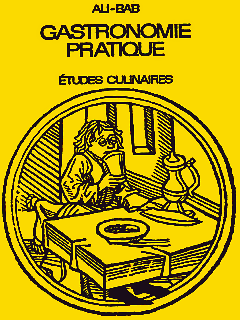
\includepdf{/other/media/Livres/Ali-Bab/images/cover_4x3.pdf}

\chapter*{\centering Introduction à la première édition}
\addcontentsline{toc}{chapter}{\scriptsize\textsc{Introduction à la première édition}}
\begin{itshape}
L'art culinaire a pour objet d'accommoder les aliments de manière à les rendre
appétissants et digestibles. Grâce à lui, nous pouvons éprouver plusieurs fois par
jour, aussi longtemps que nous sommes bien portants, des sensations agréables et,
si nous tombons malades, il facilite notre alimentation et nous permet ainsi de lutter
contre le mal en nous aidant à soutenir nos forces.

Cela suffit à montrer son importance, qui n'est cependant pas appréciée à sa
valeur, en raison des préjugés qui font généralement considérer les connaissances
humaines comme appartenant à un ordre d'autant plus élevé qu'elles sont moins
utiles. Pour ma part, j'avoue être arrivé à l'âge de vingt-cinq ans sans en avoir eu
la moindre idée et c'est seulement pendant mes premiers grands voyages, alors que,
jeune ingénieur, j'allais chercher ou étudier des gisements miniers dans des pays
perdus, que je pris goût à la cuisine. Réduits d'ordinaire, mes compagnons et moi,
aux produits de la chasse et de la pêche que les indigènes nous faisaient cuire le
plus souvent simplement grillés ou bouillis, sans autre apprêt, nous n'avions guère,
comme moyen de varier un peu nos menus, que la ressource des conserves dont on
se fatigue vite. Nous devions lutter contre l'inappétence et l'anémie qui en résulte ;
aussi la moindre innovation dans la préparation des mets était-elle accueillie avec
enthousiasme, pour peu qu'elle nous procurât une sensation gustative tranchant sur
la monotonie habituelle.

Les principes fondamentaux de l'art culinaire sont très simples. Il va sans dire
que pour faire de la bonne cuisine il est essentiel d'avoir de bonnes matières 
premières, que pour obtenir des sauces savoureuses il faut employer comme mouillement 
des jus aromatisés, du vin, des alcools de qualité convenable, enfin il n'est pas
besoin d'être très expert pour savoir que, sauf dans les cas où l'on veut saisir une
viande, il convient, le plus souvent, de faire cuire les aliments lentement, à petit
feu, en les faisant mijoter.

En appliquant ces principes, on fera toujours de la cuisine mangeable ; mais
pour faire de la cuisine fine la plupart des personnes ont besoin de guide
précis, sans quoi elles s'exposent à ne jamais arriver à préparer un plat
vraiment bien, ou, si elles y parviennent un jour par hasard, elles risquent de
ne plus le réussir le lendemain. Beaucoup d'entre elles se figurent alors qu'il
y a dans l'opération un tour de main professionnel qui leur échappe et cela les
décourage. Or, il est bien évident que pour refaire exactement ce que l'on
a fait une fois il suffit d'opérer toujours de la même manière.

Les cuisiniers habiles voient le moment précis où la cuisson est à point, ils
ont l'instinct des proportions de condiments qu'il convient d'employer et n'ont
pas besoin de se servir de balances ; mais les personnes qui n'ont pas une très
grande expérience doivent pour réussir suivre à la lettre les indications
données dans des recettes détaillées avec précision et peser tous les éléments.
Ce n'est que lorsqu'on est arrivé à être de force à se rendre compte à priori
de la valeur d’une préparation culinaire en lisant simplement sa formule, comme
un musicien expert juge un opéra sans l'avoir entendu à la seule lecture de la
partition, que l'on peut songer à voler de ses propres ailes

Un mot encore sur la genèse des plats nouveaux. Un plat est réellement nouveau
lorsque les éléments qui le composent sont associés pour la première fois, ou tout au
moins lorsque leur combinaison est faite dans des proportions inédites donnant une
saveur différente de celle des préparations connues. C'est l'étude des associations
végétales et végéto-animales qui constitue la base des créations gastronomiques. Qui
ne connaît les affinités respectives du pigeon pour les petits pois, de la perdrix pour
le chou, du gigot de mouton pour les haricots, etc., ainsi que les mets classiques
auxquels elles ont donné naissance ?

Malheureusement la découverte de ces groupements harmonieux s'est toujours
faite jusqu'à présent pour ainsi dire exclusivement par hasard et il n'y a, à vrai dire,
aucune direction à indiquer, aucune règle à formuler pour la création des plats. Seul
le goût peut amener l'artiste à des combinaisons nouvelles. Quel service rendrait à
l'Humanité le savant qui parviendrait à formuler d'une manière générale les lois des
associations eupeptiques ! Leur connaissance nous ferait probablement entrevoir des
plats que nous ne soupçonnons pas aujourd'hui, de même que les vides de la Table de
Mendéléef nous ont permis d'affirmer l'existence de corps que nous ignorions jusqu'alors.

Comme je l'ai dit plus haut, j'ai pris goût à la cuisine dans mes voyages, j'en
apprécie aujourd'hui toute la valeur et je m'en occupe volontiers à l'occasion. J'ai
modifié certains plats connus, j'en ai créé de nouveaux et, si j'en juge par les
compliments de mes amis, dont certains se piquent d'être de fins gourmets, ainsi que
par l'empressement flatteur avec lequel leurs femmes demandent mes recettes, je puis
croire que j'ai souvent réussi.

Aujourd'hui, je réunis en volume un certain nombre de ces recettes que je me suis
efforcé de rédiger d'une façon claire et précise ; j'entre, en les décrivant, dans tous
les détails nécessaires, j'indique les proportions pondérales des éléments toutes les
fois que je le crois utile, je m'attache, en un mot, à donner de véritables formules
scientifiques qui permettent de reproduire exactement les préparations décrites, sans
qu'il faille, pour les réussir, avoir de grandes connaissances culinaires ; il suffit
d'opérer soigneusement. Je mentionne dans ce recueil un certain nombre de plats très
simples, d'autres sont plus ou moins compliqués, quelques-uns sont coûteux, mais
tous peuvent être exécutés par une seule personne : c'est, en somme, de la bonne cuisine 
à la portée de tout le monde.

Comme application plus ou moins directe de l'art culinaire à la thérapeutique, j'ai
fait suivre mes formules de l'exposé d'une méthode de traitement de l'obésité des 
gourmands, sur laquelle je me permets d'attirer l'attention du lecteur. Je sais bien que je
ne satisferai pas les nombreux obèses à la recherche de la pilule miraculeuse qui les
fasse maigrir, tout en leur permettant de s'empiffrer : je prévois aussi qu'un certain
nombre de personnes diront qu'il n'y a rien de nouveau dans mon régime et qu'il est
bien certain qu'on doit maigrir en mangeant peu. Il y a cependant quelque chose de
particulier dans ma méthode. En effet, contrairement à la plupart des régimes 
alimentaires préconisés et qu'il est presque impossible d'observer longtemps, le modus
vivendi que je recommande ne fatigue pas, on peut le suivre indéfiniment sans
dégoût et j'ai obtenu en l'appliquant des résultats remarquables, tant au point de vue
de la diminution du poids, qu'à celui de l'amélioration de la santé générale, sans
faire usage d'aucun médicament.

Tous mes amis connaissent l'ancien obèse sujet principal de mon expérimentation :
ils sont prêts à témoigner de la réalité de la cure, comme ils sont prêts à attester les
qualités de ma cuisine. C'est sous leurs auspices que je présente ce livre au public.
\end{itshape}


\addtocontents{toc}{\protect\addvspace{-12pt}}%

\chapter*{\centering Préface de la troisième édition}
\addcontentsline{toc}{chapter}{\scriptsize\textsc{Préface de la troisième édition}}
La deuxième édition de ma « Gastronomie pratique » a été épuisée il y a
quelques années déjà. Des obstacles matériels en ont empêché la réimpression.

Aujourd'hui, malgré les difficultés inhérentes en ce temps à toute publication,
je présente à mes lecteurs, en les remerciant de leur bienveillance, une édition
nouvelle remaniée de fond en comble.

Ils y verront d'abord un chapitre sur le service des repas depuis les temps les
plus reculés jusqu'à nos jours, une étude succincte sur les champignons comestibles 
de France et un article documenté sur le vin qui, complétant ce qui a paru
comme généralités dans la précédente édition, font du tout un véritable Prodrome
de Gastronomie ; ils y trouveront ensuite beaucoup de formules nouvelles, ainsi
que de nombreuses indications de variantes et de créations.

L'ouvrage est devenu très volumineux, mais le serait bien davantage encore
qu'il ne pourrait contenir toutes les combinaisons culinaires qui sont
innombrables. Il n'y a pas, il n'y aura jamais de livre de cuisine complet.


\addtocontents{toc}{\protect\addvspace{-12pt}}%

\mainmatter

\newcounter{glshyperpage}%
\def\glshyper#1#2{%
\setcounter{glshyperpage}{#2}%
\addtocounter{glshyperpage}{6}%number of front-matter pages
(\hyperlink{#1.\theglshyperpage}{#2})}

\setlength{\tabcolsep}{1.5pt}
\interfootnotelinepenalty=10000  

\part*{Prodrome de Gastronomie}
\addcontentsline{toc}{part}{\protect\small PRODROME DE LA GASTRONOMIE}
\input{chapters/ch00.tex}

\addtocontents{toc}{\protect\addvspace{-5pt}}%

\chapter*{\centering La Gastronomie à travers les âges}
\addcontentsline{toc}{chapter}{\scriptsize\textsc{La Gastronomie à travers les âges (Esquisse historique)}}
L'homme ne s'est véritablement distingué des animaux que lorsqu'il a su se
servir du feu.

\index{Cuisines Antiques}

Les premiers représentants de notre espèce vivaient misérablement de fruits,
d'herbes et de racines : un peu plus tard, leurs descendants s'avisèrent de
goûter aux insectes, aux coquillages, puis à la viande, qu'ils mangeaient crue,
telle quelle, ou attendrie par des procédés primitifs, dont quelques-uns sont
parvenus jusqu'à nous\footnote{Les Huns, qui sont pour nous presque des
contemporains relativement au temps qui nous sépare des premiers hommes,
attendrissaient les viandes en s'asseyant dessus, par terre, où mieux encore
à cheval ; dans ce dernier cas ils les mettaient entre leur siège et le dos de
l'animal. Chez les Hongrois, qui descendent des Huns, le procédé ne s'est pas
perdu et pendant la révolution de 1848 les hussards de Kossuth attendrissaient
ainsi la viande avant de la faire cuire.}.

Lorsque, à la flamme du premier incendie de forêt allumé vraisemblablement par
la foudre, des animaux furent grillés, le premier homme qui mangea de la viande
cuite s'en régala sans doute, malgré le goût de brûlé qu'elle devait avoir. Dès
lors le feu fut divinisé et, tant que l'homme ne sut pas le produire
à volonté\footnote{On conçoit que les habitants de certaines contrées isolées aient pu
ignorer le feu pendant très longtemps. C'est ainsi que les indigènes des îles
Marianne, par exemple, le connurent seulement en 1521, lors de la découverte du
pays par Magellan.

Aujourd'hui, la plupart des sauvages savent faire du feu. J'ai vu les
Hottentots battre le briquet ; j'ai vu, dans l'intérieur de l'Amérique du Sud,
les Indiens allumer de la moelle d'arbre desséchée en la frottant entre leurs
mains contre une pièce de bois sec, procédé qui, par parenthèse, demande un
certain doigté pour être couronné de succès.

Néanmoins, il existe encore des peuplades très arriérées pour lesquelles la
production du feu constitue une véritable difficulté ; les indigènes de la
Terre de Feu sont dans ce cas. Il est vrai qu'au point de vue intellectuel il
n'y a guère d'être humain inférieur au Fuégien. J'en ai rencontré qui
tremblaient de froid par une température de -15° C., portant sur la tête des
peaux qu'ils allaient échanger à la côte contre des verroteries ou de
l'alcool, sans qu'il leur vint à l'esprit de se couvrir avec une partie de leur
charge.

Ces misérables représentants de notre espèce connaissent pourtant le feu, qui
leur est probablement tombé du ciel. Ils l'apprécient et s'en servent, mais ils
ne savent généralement pas le produire ; leur intelligence se borne
à l'entretenir, et c'est en cela qu'ils se montrent supérieurs aux singes dont
j'ai vu des bandes se chauffer à des feux abandonnés par des voyageurs et
qu'ils laissaient éteindre bien qu'ayant du bois coupé à côté d'eux. C'est
ainsi que dans tous leurs canots (et chaque famille de la côte a le sien qui
lui est indispensable pour la pêche) il existe un compartiment garni de terre
damée dans lequel on entretient du feu. Lorsque, par malheur, le feu s'éteint
faute de combustible, ou pour tout autre cause, les canotiers fuégiens en sont
réduits à attendre le passage d'un autre canot pour lui en emprunter. Enfin,
dans les villages de l'intérieur, il y a des feux entretenus en permanence.

Comme beaucoup de personnes, je croyais, avant d'être allé dans ce pays, que la
Terre de Feu devait son nom à des volcans visibles du large ; depuis, j'ai
changé d'avis et je suis persuadé qu'il le doit tout simplement aux feux des
canots qui, semblables à des feux follets jalonnant tout le pourtour de l'île,
ont dû frapper l'attention des premiers navigateurs qui ont doublé le cap
Horn.}, il resta le monopole des prêtres qui s'en constituèrent les gardiens.
C'est à eux que les fidèles apportaient les victimes offertes aux dieux en
holocauste : ils les faisaient cuire et… ils les mangeaient : ces prêtres
furent les premiers cuisiniers et les premiers gastronomes. Leurs descendants
spirituels ont de qui tenir.

\sk

Comme tous les arts, l'art culinaire, dont l'histoire se déroule parallèlement à
celle de l'humanité, a eu ses périodes d'éclat et ses périodes d’éclipse, et la
plupart des guerres et des grands événements politiques ont exercé une notable
influence sur son développement.

Primitif et simple chez les peuples pasteurs et chez les guerriers, luxueux et
fréquemment de mauvais goût chez les conquérants de toute sorte arrivés depuis
peu à la fortune, l'art culinaire ne devient délicat et raffiné que chez les
peuples de vieille civilisation.

Son développement général suit une courbe sinueuse. Il ne trouvera guère sa
formule définitive que lorsqu'on aura découvert toutes les lois qui le
régissent ; jusque-là, condamné à des hauts et à des bas, il sera, jouet du
hasard ou des circonstances, toujours menacé d'un retour en arrière.

\sk

\textit{Temps préhistoriques}. — La plupart des historiens se défendent de
remonter au déluge ; il me faudra cependant remonter encore plus haut. Le
déluge des Écritures ne date en effet que de {\ppp6\mmm} {\ppp000\mmm} ans
avant notre ère ; or, l'antiquité de l'homme est bien plus grande et, s'il est
difficile de la préciser, on peut du moins dire que vraisemblablement notre
espèce existe depuis un certain nombre de milliers de siècles. Quoi qu'il en
soit, l'homme quaternaire de la période paléolithique, le contemporain du
mammouth, vivait déjà de chasse et de pêche et connaissait l'usage du
feu\footnote{\label{pg0013} \hypertarget{p0013}{En ce temps-là}, les viandes étaient
généralement cuites sur des blocs de pierre chauffés au préalable. \protect Il
v a quelques années, j'ai vu employer encore ce procédé primitif de cuisson
dans les pampas de l'Amérique du Sud. Les premières choses que l'on offre dans
ces pays à un voyageur qui arrive dans une ferme sont une tasse de
\textit{maté} (infusion de feuilles d'un arbrisseau de la famille des
Illicinées) et un \textit{asado con cuerro}, c'est-à-dire du bœuf rôti dans sa
peau, qu'on prépare de la façon suivante : on commence par prendre un bœuf au
lasso, on lui coupe tête et pattes et l'on coud aussitôt les orifices pour
éviter une trop grande perte de sang ; puis on couche l'animal sur un lit de
blocs de pierre chauffés au rouge dans un feu de bois. Le rôtisseur retourne la
bête sur son lit de pierres de façon à faire cuire convenablement le filet ; le
reste est plus où moins sacrifié et beaucoup de parties sont carbonisées. Je ne
sais si c'est parce que j'ai mangé de ces asados après de longues chevauchées
et quand j'avais très faim, mais j'en ai conservé un souvenir délicieux. Je
n'oublierai jamais le flot de sang chaud qui jaillit lorsque, pour la première
fois, je plantai mon couteau dans un asado pour le découper, ni le goût exquis
du rôti ; et il me semble bien n'avoir jamais de ma vie mangé Chateaubriand
aussi juteux et aussi à point.}.
  
On en a acquis la certitude par des fragments d'ossements humains\footnote{Un
mot sur l’anthropophagie. L'homme, ayant pris goût à la viande, est devenu
cannibale le jour où il a manqué d'animaux.

« Les loups ne se mangent pas entre eux », dit-on ; si c'était vrai, ce serait
humiliant pour l'homme ; heureusement cela n'est pas ; lorsque les loups sont
affamés ils se dévorent parfaitement les uns les autres : j'ai pu m'en assurer
de visu lors d'un de mes voyages en Sibérie.

\textit{Homo hominis lupus.}

S'il est exact que « le cadavre d'un ennemi sent toujours bon », la première
victime du cannibalisme a dû être un ennemi du premier cannibale ; mais quelle
que soit la valeur de cette circonstance atténuante, c'est vraisemblablement
par gourmandise que l'homme est devenu anthropophage. Il l'est resté pour la
même raison et à d'autres points de vue : par superstition, dans la pensée
qu'il hériterait ainsi des qualités de la victime, par vengeance, et même
quelquefois par respect pour les morts, auxquels il croyait assurer de la sorte
la plus honorable des sépultures.

Le développement de la morale d'un côté et l'élevage du bétail de l'autre l'ont
corrigé de cette habitude ; mais il est prêt à y revenir dès que son existence
entre en jeu : l'histoire du radeau de la Méduse se renouvelle de temps en
temps.

Malgré le développement de la civilisation, il existe encore nombre de
peuplades anthropophages.

Des indigènes de la côte de Krou, en Afrique, qui avaient mangé des prisonniers
faits dans les combats que les tribus sauvages se livrent entre elles, le plus
souvent pour se procurer de la nourriture, m'ont dit en avoir conservé un
excellent souvenir, « Li semblé cochon » ; et il est effectivement assez
naturel que la chair des deux omnivores soit analogue. Un jour, l'un de ces
Kroumen, en veine de confidences, revenant sur le même sujet et précisant ses
impressions, me dit en riant d'un rire large qui découvrait toutes ses dents :
« Blanc pas bon ; mo pli content nég ». Il parait en effet que la chair du blanc
est plutôt fade. C'est aussi l'avis des tigres du Bengale qui ont une certaine
compétence en la matière, et qui, ayant à choisir entre un blanc et un hindou,
n'hésitent jamais à prendre le second. C'est l'une des raisons pour lesquelles
les Européens emmènent toujours des Hindous avec eux à la chasse au tigre.

Faut-il le dire ! J'ai moi-même compris l'anthropophagie dans un de mes voyages
où, après être resté vingt-quatre heures sans rien prendre, par suite de la
perte de toutes mes provisions au passage d'un saut de rivière, j'ai mangé pour
la première fois du singe. Cet animal, gros comme un enfant, qu'on faisait
rôtir à la broche, me donna l'impression que j'allais manger mon semblable.} et
d'os d'animaux calcinés trouvés dans les cavernes de cette époque et par les
\textit{kjoekkenmoeddings}\footnote{ Les kjoekkenmoeddings ont été trouvés pour
la première fois au bord de la mer, en Danemark, d'où leur nom danois qui
signifie résidus de cuisine, puis ailleurs, un peu partout, en Europe : en
France, en Belgique, en Allemagne, en Angleterre, au Portugal ; en Asie : au
Japon ; et dans les deux Amériques,

Les différents kjockkenmoeddings ne datent pas tous de la même époque. Mon
savant camarade et ami de Morgan, dans son magistral ouvrage : « les premières
civilisations  », rapporte les kjockkenmoeddings danois à l'état mésolithique,
intermédiaire entre l'état paléolithique et l'état néolithique ou celui de la
pierre polie ; tandis que les kjockkenmoeddings portugais par exemple seraient
franchement néolithiques. }, vestiges d'anciennes agglomérations humaines
renfermant des instruments de silex, des fragments de poterie grossière, du
charbon, des cendres, des os calcinés et brisés, des coquilles marines, des
arêtes de poissons, etc.

Les premiers animaux domestiques paraissent avoir été le chien, le renne, la
chèvre, le porc et la poule.

C'est également de la fin de la période de la pierre taillée (phase
néolithique) et de l'époque des cités lacustres que datent l'élevage du bétail,
la culture des céréales, le tissage, l'emploi du miel et l'usage du
sel\footnote{La découverte du sel est l’une des plus précieuses au point de vue
gastronomique. Les propriétés de ce condiment sont nombreuses : Il stimule
l'appétit, provoque la salivation, active la circulation du sang dans la
muqueuse stomacale, facilite la digestion en fournissant par sa décomposition
l'acide chlorhydrique nécessaire au suc gastrique ; et ainsi, d'une façon
générale, il contribue à l'équilibre de notre statique chimique ; de plus, il
favorise l'oxygénation du sang, ravive la couleur des globules sanguins, il est
antiseptique, etc., etc. Indispensable à la vie animale, il se trouve à l'état
naturel dans la plupart de nos aliments, mais en proportion insuffisante, au
moins pour notre organisation actuelle. Le manque de sel est l'une des
privations physiques les plus pénibles. Les personnes soumises au régime
déchloruré ne peuvent s'en faire qu'une faible idée, car les ressources
actuelles de la gastronomie permettent d'y suppléer, en partie au moins, grâce
à des artifices culinaires et à d'autres condiments. Pour s'en rendre compte
exactement, il faut, comme cela m'est arrivé, en avoir été privé pendant
longtemps sans rien avoir à lui substituer. C'est ainsi qu'à la suite de
l'accident du canot, dont j'ai dit un mot dans la note {\ppp2\mmm} de la page
{\ppp13\mmm}, j'ai vécu exclusivement pendant tout un mois, dans les forêts de
la Guyane, de gibier et de poisson rôtis au naturel, sans aucun assaisonnement.
Le manque de sel m'avait fait prendre la nourriture en tel dégoût que je ne
mangeais presque plus. Aussi, à ce régime, je m'étais anémié au point que je
fus littéralement étourdi et obligé de me coucher, au premier petit verre de
vin que je pris à la fin de mon jeûne forcé. Mon appétit revint dès le premier
repas assaisonné et, quelques jours après, j'avais repris mes forces.}.

\sk

\textit{Antiquité. — Égyptiens. —} Sous les Pharaons de la
IV\textsuperscript{e} dynastie, {\ppp3\mmm} {\ppp000\mmm} ans avant notre ère,
en Égypte, berceau de la civilisation, on cultivait déjà le froment, l'orge, le
millet, la vigne : on faisait du pain, du vin, de l'hydromel, de la bière.

Mille ans plus tard, sous la XVIII\textsuperscript{e} dynastie, celle des
grands Pharaons, époque où l'Égypte atteignit son apogée, la conquête de la
Syrie, de la Phénicie, du pays de Chanaan, de la Nubie et de l'Éthiopie
augmentèrent les ressources culinaires des Égyptiens. À cette époque, ils se
nourrissaient de viande de boucherie, de volaille, de gibier, de poissons,
d'huîtres, d'œufs\footnote{On savait déjà à cette époque faire éclore
artificiellement les œufs.}, de légumes farineux : lentilles, pois, fèves,
etc., de fruits variés : olives, figues, dattes, pommes, grenades, abricots,
amandes, etc. ; ils connaissaient l'ail, le persil ; ils adoraient l'oignon et
le mangeaient avec un respect religieux. Thèbes aux cent portes avait ses
éleveurs de volaille, ses gargotiers, ses confiseurs, ses pâtissiers, et l'on
voyait sur la table des Pharaons des truffes merveilleuses, de dimensions
inouïes, dont le poids atteignait {\ppp36\mmm} kilogrammes. Cette espèce semble
disparue de nos jours.

\sk

\textit{Hébreux}. — À l'origine, les Hébreux vivaient très frugalement. Plus
tard, ils menèrent la vie des patriarches : ils se nourrissaient de céréales :
blé, orge ; de quelques légumineuses : lentilles, fèves, et de la chair de
leurs troupeaux.

Lors de leur séjour en Égypte, leur alimentation s'augmenta de tous les
produits qu'ils trouvèrent dans le pays. Vingt siècles avant notre ère ils
connurent le beurre.

Puis, durant les quarante années pendant lesquelles ils errèrent dans le désert
({\ppp1\mmm} {\ppp420\mmm}-{\ppp1\mmm} {\ppp380\mmm} avant Jésus-Christ), ils eurent
beaucoup à souffrir, mais leur plus grande privation fut de n'avoir pu
emporter, en fuyant d'Égypte, ni graines d'oignon, ni levure. C'est de cette
époque que date l'usage du pain azyme que les Juifs pratiquants mangent encore
à Pâques, en souvenir à la fois de l'ancienne fête des azymes et du séjour des
Hébreux dans le désert.

Après leur entrée dans la terre de Chanaan, la nourriture des Hébreux se
modifia. Pour obéir aux lois de Moïse, ils rejetèrent de leur alimentation
beaucoup d'animaux dont ils faisaient jadis usage, et le beurre fit place à la
graisse et à l'huile.

Ce fut l'origine de la cuisine juive\footnote{Voir \hyperlink{p0045}{p. {\ppp\pageref{pg0045}\mmm}.}}

Cependant, sous le règne de Salomon au luxe proverbial, les Hébreux,
transgressant les préceptes de la religion, poussèrent la richesse et la
somptuosité de la table à un tel degré que le prophète Isaïe s'en émut et s'en
indigna.

\sk

\textit{Assyriens. Chaldéens}. — Les Assyriens s'occupaient peu de travaux
agricoles ; ils tiraient de leur sol quelques produits sauvages, mais ils
vivaient surtout aux dépens des peuples voisins.

Les Chaldéens, au contraire, s'occupaient beaucoup de culture, ainsi que le
prouve la flore si riche des jardins suspendus de Babylone.

En Assyrie, la classe pauvre se nourrissait de pain grossier, de légumes
sauvages, de tourteaux de poissons et de sauterelles. Dans la classe riche la
table était plus abondamment pourvue ; on y voyait des viandes, les mêmes que
celles d'Égypte, des poissons, dont les plus estimés étaient la carpe, le
barbeau, l'anguille et la murène ; des herbes potagères, des légumes variés :
haricots, fèves, lentilles, pois chiches, gombos, concombres, courges,
aubergines, etc., des fruits : raisin, dattes, ananas, mûres, amandes,
pistaches, noix, figues, grenades, citrons, oranges, poires, prunes, abricots,
etc.

Après chaque victoire, les Assyriens se vautraient dans l'orgie, mais ce fut
seulement au \textsc{vii}\textsuperscript{e} siècle avant notre ère, sous le
règne d'Assurbanipal, que Ninive et Babylone atteignirent l'apogée de leur
splendeur et que l'amour du luxe et des plaisirs matériels fut poussé au plus
haut point. Enfin, au \textsc{vi}\textsuperscript{e} siècle, sous le règne de
Balthasar, de crapuleuse mémoire, les Assyriens sombrèrent dans la plus
répugnante débauche.

\sk

\textit{Hindous}. — Dans l'Inde, d'où nous viennent le riz et des condiments de
haut goût, l'art culinaire était très développé dès la plus haute antiquité,
ainsi qu'en témoigne le « Rāmāyana  », ancienne épopée hindoue consacrée à la
glorification du héros Rāma.

\sk

\textit{Perses}. — Les Perses, d'origine aryenne comme les Hindous, étaient dès
les temps les plus reculés un peuple d'agriculteurs.

Au \textsc{ix}\textsuperscript{e} siècle avant Jésus-Christ, leur nourriture se
composait de céréales, de plantes légumineuses, d'herbes potagères et de fruits
tels que raisin, olives, citrons, cerises, prunes, pêches, noix ; les viandes
dont ils faisaient usage étaient celles du cerf, de l'âne sauvage, du bœuf, du
mouton, du porc, de l'autruche et de la tortue de mer.

A la suite des victoires qu'ils remportèrent sur Nabuchodonosor et sur
Balthasar, et après la conquête de l'empire des Mèdes, de l’Assyrie, de la
Chaldée, de la Lydie, de l'Inde, etc., les Perses, au contact des vaincus,
prirent des habitudes de luxe et d'intempérance. A la table des rois et des
riches on servait entiers de gros animaux rôtis, un chameau, un bœuf, un âne ;
chez les pauvres on se contentait de pièces plus petites.

Au \textsc{v}\textsuperscript{e} siècle, après les guerres médiques, pendant
lesquelles ils abandonnèrent souvent aux Grecs vainqueurs des richesses inouïes
en vaisselle et en mobilier d'or et d'argent, les Perses suivirent l'exemple
des Égyptiens, des Assyriens et des Hébreux ; ils se laissèrent aller à la
mollesse et à la volupté ; la débauche envahit tout : ce fut le commencement de
la décadence.

\sk

\textit{Grecs}. — En {\ppp1\mmm} {\ppp582\mmm} avant Jésus-Christ, Cécrops,
fondateur d'Athènes, y apporta d'Égypte les olives et l'art d'en faire de
l'huile. Vers la même époque, le phénicien Cadmus, cuisinier du roi de Sidon,
vint s'établir en Grèce et y introduisit les principes de l'art culinaire.

Au temps d'Homère, la nourriture du peuple était presque exclusivement composée
de bouillies de céréales, de poissons, de légumes et de fruits du pays.

La classe riche y adjoignait du bœuf, du mouton, de la chèvre et du porc : on
faisait rôtir ces animaux en les arrosant de graisse\footnote{ C'est encore
cette méthode de cuisson qu'on emploie de nos jours dans l'intérieur de la
péninsule balkanique. L'animal vidé, parfumé d'un bouquet de thym et embroché
sur une branche de coudrier, est rôti devant un grand feu de bois. Pendant la
cuisson, le Palikare rôtisseur trempe, de temps en temps, dans de la graisse
fondue assaisonnée et relevée par un peu de jus de citron, un petit drapeau de
toile et en caresse légèrement le rôti, d'autant plus fréquemment que la viande
se dore davantage. Ce procédé de graissage est très recommandable ; il a pour
effet d'éviter le ramollissement de la viande et il donne à la peau une
consistance croustillante très agréable.

Le méchoui arabe est préparé d'une façon analogue.} et on les mangeait en
buvant des vins aromatisés.

La gastronomie, marchant de pair avec la civilisation, commençait à se
développer, lorsque survint l'invasion dorienne qui arrêta tout progrès. Ce fut
alors que Lycurgue, qui voulait faire des Spartiates exclusivement un peuple de
soldats, essaya, en n'accordant à chacun d'eux qu'un minimum de jouissances
égal pour tous, de leur inculquer avec l'amour immodéré des armes le plus
profond mépris pour tous les arts : et, afin d'atrophier en eux le sens du
goût, il ne trouva rien de mieux que son fameux brouet\footnote{Le brouet noir
était un ragoût au vinaigre de viandes plus ou moins carbonisées, accompagnées
de plantes aromatiques et amères.}, qu'il eut la prétention de rendre sinon
gratuit, du moins obligatoire. C'en était trop ; les estomacs se révoltèrent, et
Lycurgue ne survécut pas à cet échec.

Après sa mort, les Lacédémoniens, trouvant que leur diète avait assez duré,
entreprirent les guerres de Messénie à seule fin de s'emparer des troupeaux et
des récoltes de leurs voisins. A la suite de ces conquêtes la cuisine grecque
s'améliora ; elle dut aussi ses progrès à l'influence d'Archestrate, l'immortel
auteur de la « Gastrologie », ouvrage qu'il écrivit après avoir parcouru le
monde connu, à la recherche de tout ce qu'il pouvait y avoir de meilleur
à boire et à manger. L'alimentation s'enrichit alors notablement par l'emploi
du seigle, du riz, de l’avoine : on vit apparaître sur les tables les
volatiles, les poissons, les légumes et les fruits les plus variés ; les
préparations culinaires furent relevées par de nombreux condiments ; on peut
citer, outre ceux déjà mentionnés : le poireau, la ciboule, la câpre, le
raifort, le thym, la sauge, l'origan, la coriandre, le fenouil, etc.

C'est en vain que le végétarien Pythagore prêcha, sous prétexte de
métempsychose, l'abstinence des viandes, la gastronomie, étouffée pendant
plusieurs siècles, triompha de la philosophie et reprit irrésistiblement son
essor.

Au \textsc{v}\textsuperscript{e} siècle avant notre ère survinrent les guerres
médiques et leur principal résultat fut l'introduction en Grèce des
connaissances culinaires déjà assez développées chez les Mèdes et chez les
Perses.

Au siècle de Périclès, les menus comprennent des potages, des poissons rôtis,
frits ou bouillis, ceux-ci accompagnés d'une sauce à l'huile (avec vinaigre,
jaunes d'œufs et fines herbes), origine de notre rémoulade : des viandes de
boucherie et de porc ; de la volaille, en particulier l'oie blanche engraissée
avec des figues fraîches, très recherchée pour sa chair, son foie, sa
graisse\footnote{Les Grecs ne connurent le beurre que très tard, par les
Scythes, qui en fabriquaient de toute antiquité.} et ses œufs ; du gibier rôti,
braisé ou en ragoût, le tout relevé par des sauces diverses, les unes douces
à base de miel, les autres piquantes à base de vinaigre : des légumes, des
desserts variés, des fruits de toute sorte, des fromages\footnote{Notamment
ceux de Sicile et ceux de la ville de Tromilée, en Arcadie.}, des pâtisseries,
parmi lesquelles certains gâteaux saupoudrés de sel, que l'on fabrique encore
de nos jours : enfin des entremets sucrés, dont quelques-uns étaient les
premières ébauches du pudding.

Comme boisson, les Grecs faisaient usage de lait, de vins indigènes ou
étrangers naturels, cuits ou fumés, d'hydromel, de cervoise\footnote{Boisson
analogue à la bière.}, de bière, de tisanes. Les vins indigènes les plus
appréciés étaient ceux de Corinthe, d'Acanthos et des Îles Ioniennes ; les vins
étrangers, ceux de Syracuse, de Falerne, de Smyrne, de Phénicie, d'Égypte et en
particulier ceux de la Thébaïde.

Le déjeuner du matin et celui de midi étaient sommaires ; en revanche le dîner
était copieux et se composait de plusieurs services. Dans ces repas du soir,
avant le dessert, des esclaves apportaient aux convives de l'eau, des parfums,
des couronnes de fleurs et de feuillage. C'est seulement alors que l’on
commençait à verser à boire. Puis, pendant le dessert, il y avait des
représentations mimiques, des lectures, des chants, des danses : des musiciens
se faisaient entendre, et les convives, excités par la boisson, déployaient
leur verve dans de joyeuses conversations et dans des saillies épicées de sel
attique.

Ces réunions étaient surtout un régal pour l'esprit ; mais la préparation des
mets laissait à désirer, et il faut bien dire que les Grecs, à cette époque qui
marque l'apogée de leur civilisation, n'avaient pas poussé la
gastronomie\footnote{On trouve dans Aristophane l'indication de nombreuses
substances alimentaires employées de son temps. Je crois intéressant d'en faire
l'énumération. Comme viandes de boucherie : l'agneau, le baudet, la brebis, le
cochon de lait et la truie ; comme issues et charcuterie : l'andouille, le
boudin, la saucisse et les tripes ; comme volaille : la poule, le canard, l'oie
et le pigeon ; comme gibiers : le lièvre, l'alouette, le bec-figue, la caille,
la grive, la perdrix, le faisan, la poule d'eau, la sarcelle et l'autruche ;
comme poissons : l'anguille, la loche, le maquereau, le mulet, la plie, la
raie, le rouget, la sardine, le thon et le turbot ; comme crustacés et
mollusques : le crabe, la crevette, l'écrevisse et l'huître ; comme insectes :
les sauterelles ; comme reptiles : la tortue ; comme grains : le blé, l'orge ;
comme légumes secs : la fève, les haricots, les lentilles, les pois et les pois
chiches ; comme légumes frais et condiments : l'ail, l'anis, la bette, la
betterave, le cardon, la ciboule, la citrouille, le concombre, la coriandre, le
cresson, la faîne, l'oignon, l'olive, le persil, le poireau, le raifort, la
rave, le sésame, le thym ; comme fruits : les figues, les grenades, l'orange,
la poire, la pomme et le raisin.

Ajoutons qu'Aristote mentionne dans son « Éthique » vingt variétés de coulis.}
aussi loin que les autres arts.

Cependant il se manifestait depuis quelque temps déjà des symptômes de
décadence. Les Grecs avaient pris chez les Libyens la déplorable habitude de
manger couchés, première erreur gastronomique ; ils tombèrent ensuite dans une
seconde plus grave, celle de vivre pour manger. En vain Hippocrate, au nom de
l'hygiène, et Socrate, au nom de la morale, s'efforçaient-ils de lutter contre
l'envahissement de la goinfrerie ; la Grèce déclinait de plus en plus et, un
siècle après Périclès, en {\ppp146\mmm} avant J.-C., elle fut asservie par
Rome.

\sk

\textit{Romains}. — Les Romains des premiers âges, comme tous les peuples
primitifs, menaient une existence misérable. Numa Pompilius emprunta aux Sabins
qui le tenaient eux-mêmes des Perses, par l'intermédiaire des Pélages, le culte
de Vesta déesse du feu ; de cette époque (\textsc{vii}\textsuperscript{e}
siècle av. J.-C.) datent les commencements de l'art culinaire à Rome.

Au début, les Romains ne mangeaient guère de viande que les jours de fête, et
leur nourriture ordinaire consistait surtout en végétaux, ail, oignons, légumes
à cosses, navets, panais, poireaux, etc. ; et la bouillie
d'épeautre\footnote{Variété de froment qui pousse dans les terrains arides.}
faisait office de pain.

A l’origine, ils castraient les taureaux uniquement pour les dompter avec plus
de facilité. Mais bientôt ils s'aperçurent que cette opération améliorait
singulièrement la qualité de la viande, et cela leur donna par la suite l'idée
de chaponner les coqs. Telle fut chez eux l'origine de l'élevage.

Ils connurent la vigne par les Phocéens, qui la leur apportèrent de Perse.

Les guerres du Samnium mirent les Romains en contact avec les Grecs, alliés des
Samnites ; c'est à leur école qu'ils apprirent les principes de l'art culinaire.
Toutefois ce ne fut qu'à l'époque des guerres puniques\footnote{ Flaubert, dans
le premier chapitre de « Salammbô  », rapporte des détails précis sur cette
époque. Je crois intéressant de citer \textit{in extenso} la description qu'il
y a faite du festin donné dans les jardins d'Hamilcar pour célébrer
l'anniversaire de la bataille d'Eryx.

« Les cuisines d'Hamilcar n'étant pas suffisantes, le conseil leur avait envoyé
des esclaves, de la vaisselle, des lits, et l'on voyait au milieu du jardin,
comme sur un champ de bataille quand on brûle les morts, des grande feux clairs
où rôtissaient les bœufs. Les pains saupoudrés d'anis alternaient avec les gros
fromages plus lourds que des disques et les cratères pleins de vin, et les
canthares pleines d'eau auprès des corbeilles en filigrane d'or qui contenaient
des fleurs. La joie de pouvoir enfin se gorger à l'aise dilatait tous les
yeux ; çà et là les chansons commençaient.

D'abord on leur servit des oiseaux à la sauce verte, dans des assiettes
d'argile rouge rehaussée de dessins noirs, puis toutes les espèces de
coquillages que l'on ramasse sur les côtes puniques, des bouillies de froment,
de fève et d'orge et des escargots au cumin, sur des plats d'ambre jaune.

Ensuite les tables furent couvertes de viandes : antilopes avec leurs cornes,
paons avec leurs plumes, moutons entiers cuits au vin doux, gigots de chamelles
et de buffles, hérissons au garum, cigales frites et loirs confits. Dans des
gamelles en bois de Tamrapanni flottaient, au milieu du safran, de grands
morceaux de graisse. Tout débordait de saumure, de truffes et d'asa fœtida. Les
pyramides de fruits s'éboulaient sur les gâteaux de miel et l'on n'avait pas
oublié quelques-uns de ces petits chiens à gros ventre et à soies roses que
l'on engraissait avec du marc d'olives, mets carthaginois, en abomination aux
autres peuples. »} que la gastronomie fit vraiment à Rome des progrès sérieux.

La première guerre leur donna la Sicile, dont les cuisiniers\footnote{Les
cuisiniers siciliens, dont les premiers étaient d'origine grecque, ont joué un
rôle considérable dans l'histoire de Rome. C'était eux qu'Annibal, imprudent,
emmenait avec lui en campagne. Pendant la deuxième guerre punique, ils le
plongèrent à Capoue dans de telles délices qu'il s'y attarda avec son armée et
finit par se faire battre, tandis qu'en opérant rapidement il aurait pu,
dit-on, s'emparer de Rome qui était alors à deux doigts de sa perte.} (quantum
mutati) étaient alors les premiers du monde.

La deuxième leur valut les îles Baléares, où ils trouvèrent le lapin qu'ils
s'empressèrent d'acclimater dans leur pays.

On sait comment la troisième, celle qui se termina par la destruction de
Carthage, fut provoquée par Caton l'Ancien. Pendant la délibération, quelques
sénateurs hésitaient. Caton tira de sa toge des figues d'Afrique et s'écria :
« C'est la conquête du pays producteur de ces fruits que je demande. »
L'argument fut irrésistible.

C'est de celle même époque que date l'introduction de la grenade.

Plus tard, l'annexion de la Grèce apporta aux Romains de nouvelles conquêtes
gastronomiques. Ils trouvèrent dans ce pays le faisan que les Argonautes
avaient rapporté de leur expédition sur les bords du Phase, la bécasse et
d'autres gibiers dont nous avons déjà parlé, des légumes variés parmi lesquels
nous citerons, outre ceux mentionnés plus haut, l'asperge, la carotte, le
cerfeuil, les champignons, la laitue, le pissenlit, la truffe, originaire de
Libye, et des fruits tels que la noix et la pêche qui venaient de Perse.

D'Asie, ils avaient rapporté la cerise\footnote{La cerise fut importée par
Lucullus, de Gérasonte, ville de Pont.}, l'abricot\footnote{L’abricot fut
importé d'Arménie.}, le concombre, le citron\footnote{Le citron ne paraît avoir
été introduit à Rome que postérieurement à Pline.}, le paon\footnote{Le paon
fut importé de Samos par Hortensius.} ; et les Parthes leur avaient enseigné la
fabrication du pain mollet. D'Afrique, leur vint le melon à grosses côtes
qu'ils se mirent à cultiver près du village de Cantalupe, d'où le nom de
cantaloup.

Ils pêchaient dans leurs rivières et dans leurs deux mers des ablettes, des
anchois, des bars, des barbillons, des daurades, des esturgeons, des harengs,
des mulets, des murènes, des turbots, des grenouilles, des moules, des huîtres,
des oursins, des palourdes. Le gibier ne leur manquait pas non plus. Ils élevaient
le gibier à poil dans des parcs, le gibier à plumes dans des volières, dont la
première fut construite par Marcus Lœnius Strato.

C'est Sergius Orata qui eut le premier l'idée de parquer les huîtres, et les
parcs du lac Luerin fournissaient des mollusques à point : Fulvius Lippinus
avait imaginé d'engraisser des escargots avec une bouillie faite de farine et
de moût de vin et il obtenait ainsi des produits hors ligne ; le consul Scipio
Metellus, promoteur du gavage des oies dans l'obscurité, avait créé le foie
gras. Les Romains, très versés dans l'art de la charcuterie, obtenaient des
truies à chair très parfumée en les nourrissant de figues\footnote{On conçoit
parfaitement que les animaux ainsi nourris devaient être exquis. En Espagne,
dans la province de Séville, on donne à manger aux porcs des glands et des
olives, et l'on obtient ainsi une chair excellente.} ; ils préparaient des
jambons, des saucisses, etc. Ils accommodaient en salade le cresson, la laitue,
l'oseille, la manne, la rue. Ils faisaient certains fromages\footnote{Dans ses
ouvrages. Martial signale parmi les fromages connus de son temps ceux de Luna,
en Étrurie, ceux de Vélabre, qui étaient durcis au feu, et ceux de Toulouse.}
dans la composition desquels entrait souvent du thym en poudre. Ils
confectionnaient couramment de la crème fouettée, des oublies, des tourtes, des
croûtes, des puddings, des gâteaux au fromage, des sorbets, etc. Ils avaient
aussi une très grande variété de fruits : pommes, poires, prunes, châtaignes,
coings\footnote{Importé de Syrie du temps de Galien.}, raisin,
pistache\footnote{Importée de Syrie par Vitellius.}, etc.

En fait de vins\footnote{ Martial cite les vins de Campanie, de Cécube, de
Céré, les vins miellés de Crète, les vins de Falerne, de Fondi, de Mammerte, de
Marseille, des Mares, de Nomentanum, de la Sabine, de Sitie, de Sigui, de
Sorrente, de Spolète, de Tarragone et de Toscane.

Les Romains employaient volontiers comme boisson, pure ou coupée de vin, de
l'eau glacée qu'ils avaient fait bouillir au préalable, par une sorte de
prescience très curieuse de l’asepsie, fondée peut-être sur le vieil adage :
« le feu purifie tout ».}, ils avaient les vins connus des Grecs, les leurs et
ceux du Rhin,

Leurs ressources gastronomiques considérables et leurs connaissances culinaires
relativement\footnote{ Comme les Grecs, les Romains ne connurent le beurre que très
tard ; ils le trouvèrent chez les Germains. Leur cuisine était préparée
à l'huile et à la graisse, comme cela se fait encore de nos jours dans le Midi,

Parmi les plats les plus renommés de l’époque, il faut citer les tétines de
truie à la saumure de thon, les pâtés de volaille, les grives aux asperges, le
porc à la Troyenne farci de bec-figues et d'huîtres, le tout arrosé de vin et
de jus aromatisé.} étendues leur avaient permis de créer une cuisine plus
raffinée que la cuisine grecque ; malheureusement ils finirent par devenir trop
carnivores et ils eurent le tort de méconnaître la valeur des
légumes\footnote{Les Romains de la classe aisée n'estimaient guère que les
légumes plus ou moins rares, les grosses asperges, les choux nains, les cœurs
de laitue, qu'ils mangeaient trempés dans de la crème ou dans du garum de
maquereau, et les champignons.}, qu'ils trouvaient fades, alors que les Grecs,
plus délicats, avaient su les apprécier. Les repas romains, très somptueux,
étaient égayés par des représentations théâtrales et musicales\footnote{Martial
écrivait à ce sujet : « Vous me demandez quel est le meilleur festin ? C'est
celui où il n'y à pas de joueur de flûte ». Ceux qui, de nos jours, inscrivent
sur leurs programmes comme \textit{great attraction} : « Pas de Tsiganes »,
appartiennent, sans s'en douter, à l'école de Martial.}, mais, contrairement
à ce qui se passait en Grèce, les convives restaient spectateurs passifs de ces
divertissements.

En résumé, les Romains jouissaient d’un très grand bien-être matériel, mais la
facilité avec laquelle ils s'étaient enrichis par le pillage des contrées
conquises, les conduisit et devait fatalement les conduire à des excès de toute
sorte : aussi ils marchèrent à grands pas vers la décadence et ils finirent par
ne plus vivre que pour satisfaire leur gloutonnerie. L'introduction de l'usage
immonde du vomitorium marque la fin de la gastronomie romaine. Un véritable
vent de folie souffla alors sur Rome. Ce fut à qui dépenserait le plus. On
rivalisait de plats rares et le plus souvent insensés\footnote{Dans son
« Satyricon », Pétrone parle de plusieurs plats de cette catégorie en décrivant
une orgie chez Trymalcion, qui paraît être une critique de la fameuse orgie que
Néron, ce Nabuchodonosor romain, donna sur l'étang d'Agrippa. Citons entre
autres une laie en surprise, invraisemblable pièce montée, composée d'une
énorme laie en peau, portant à chacune de ses défenses une corbeille tissue de
petites branches de palmier et contenant l'une des dattes de Syrie, l'autre des
dattes de la Thébaïde, et autour de laquelle étaient groupés, en nombre égal
à celui des convives, des marcassins en pâte cuite. Lorsque l'écuyer tranchant
ouvrit la laie, il s'en échappa un vol de grives que les esclaves attrapèrent
à la glu. Chacun des convives reçut un marcassin en pâte, des grives en vie et
des dattes. Un autre plat en surprise était une truie à ventre rebondi, farcie
de boudins et de saucisses, que le cuisinier apportait en s'excusant d'avoir
oublié de la vider. Signalons encore une faisane en plumes, couvant des œufs en
pâte farcis d'une purée de jaunes d'œufs durs masquant des bec-figues rôtis.
Les surprises modernes sont incontestablement de meilleur goût à tous les
points de vue, et il me suffira de citer à cet égard les ortolans en
sarcophages, qui se présentent sous la forme de truffes farcies chacune d'un
ortolan, garni lui-même de foie gras, et qui laissent loin derrière ceux les
œufs de faisane dont je viens de parler.}. On servait des talons de chameau,
des trompes d'éléphants, des têtes de perroquets, des ragoûts de foies de
rossignols et de cervelles de paons, et des pâtés de langues d'oiseaux savants
qui atteignaient des prix équivalant à {\ppp20\mmm} {\ppp000\mmm} francs de
notre monnaie. Lucullus\footnote{Lucullus, qui s'était scandaleusement enrichi
dans ses campagnes en Cappadoce contre Mithridate, jetait littéralement
l’argent par les fenêtres. Il payait {\ppp20\mmm} {\ppp000\mmm} francs par an
ses écuyers tranchants. Dans la seule baie de Naples, il possédait trois
châteaux autour desquels il y avait des parcs et des volières regorgeant de
gibier et de volaille, des viviers pour poissons d'eau douce et d'autres pour
poissons de mer. Pour alimenter ses viviers d'eau fraîche, il avait fait percer
toute une chaîne de collines, ce qui était pour l’époque un travail colossal.}
dépensait {\ppp50\mmm} {\ppp000\mmm} francs en un seul repas. Sous le règne de
Tibère, Marcus Apicius\footnote{Ce fut lui qui imagina de noyer les rougets
dans le garum (apéritif aphrodisiaque, d'origine grecque, à base de saumure de
poisson) et de les préparer ensuite avec une sauce dont le fond était leur
propre foie. Le principe de cette sauce a survécu. De nos jours on sert les
rougets grillés masqués d'une purée faite avec leurs foies et du beurre.},
possesseur d'une fortune représentant cinquante millions de francs, trouvait le
moyen d'en gaspiller les trois quarts en orgies et finissait par le suicide,
estimant qu'il n'avait plus de quoi vivre décemment. Vitellius, qui ne
s'interrompait de manger que pour vomir, dévorait quatre-vingts millions en
huit mois de règne. Héliogabale, à peine âgé de {\ppp18\mmm} ans, dépassait en
débauche et en prodigalités les Césars ses prédécesseurs. Désireux de passer
à la postérité sous son vrai jour, il avait un historiographe attaché à sa
personne pour décrire ses orgies. Il donnait des festins comprenant jusqu'à
vingt-deux services ; et, pour augmenter la dépense, il faisait mélanger aux
plats servis à ses invités des perles, de l'or et des pierres précieuses.
Passons !

\sk

\textit{Invasion des Barbares}. — L'odeur des saturnales romaines se répandit
au loin : elle finit par attirer les Barbares, dont les invasions durèrent près
de trois siècles et plongèrent dans une nuit profonde la civilisation du monde
antique qui se mourait d'indigestion.

Foulées sous les pieds des Barbares, les truffes s'enfoncèrent dans le sol et
disparurent ; elles ne reparaîtront qu'à l’époque de la Renaissance.

Les savants, les penseurs, les artistes, traqués par les envahisseurs, se réfugièrent
dans les couvents alors regardés comme inviolables.

\sk

\textit{Christianisme}. — Sous l'influence du Christianisme, l’art culinaire se
simplifia dans les couvents et, après une phase de rigoureux ascétisme, il
redevint, ce qu'il n'aurait jamais dû cesser d'être, l'art de rendre les
aliments appétissants et digestibles. Le développement du jardinage, favorisé
par la vie monastique, introduisit dans la nourriture des légumes et des
fruits. L'institution très hygiénique des jours maigres enrichit de nouveaux
plats le répertoire de la cuisine païenne. Les jeûnes et les abstinences
reposèrent les estomacs et leur firent apprécier la cuisine simple.

Dans tous les monastères, les religieux devaient, par principe égalitaire,
vaquer à tour de rôle à la confection des mets ; ce fut l'origine de nombreux
progrès gastronomiques, car il se trouvait parmi les moines des gens de goût
que l'émulation conduisit tout naturellement à perfectionner les formules
anciennes. La cuisine des couvents fut toujours bonne, grâce à l'excellence des
matières premières employées et aux soins apportés à leur préparation, et il
est indiscutable que c'est à eux que nous devons la conservation et le
développement des principes rationnels de la science gastronomique.

\sk

\index{Cuisine française depuis les origines jusqu'à nos jours}

\textit{Gaule}. — Avant d'aller plus loin, retournons un peu en arrière et
disons un mot des Gaulois.

Dans la période qui précéda la conquête romaine, les Gaulois vivaient de
pain\footnote{Ce sont les Phéniciens qui introduisirent le blé à Marseille.} de
laitage, d'œufs, de légumes. d'oignons cuits sous la cendre, de viandes de
boucherie et de porc, ainsi que de gibier, de poissons, assaisonnés de sel, de
safran, de miel, de vinaigre et de brou de noix. Ils buvaient de l'hydromel, de
la bière et du vin\footnote{La vigne fut importée à Marseille, avant la
conquête des Gaules, par un Toscan banni de sa patrie.}

Les différentes invasions modifièrent beaucoup leur cuisine. Après la conquête
romaine le nombre des services s'accrut, le luxe se manifesta par la variété
des mets et des assaisonnements relevés, mais l'invasion des Huns, qui
mangeaient la viande à moitié crue et aux trois quarts corrompue, arrêta cet
élan et il faut arriver à l'époque des Francs pour retrouver une nourriture
quelque peu soignée.

\sk

\textit{Gaule franque}. — A l’époque des Mérovingiens, de nouvelles créations
culinaires apparurent. Un certain nombre de mets comprenaient des sauces au
bouillon, au vin, aux plantes aromatiques : on préparait au jus de viande
beaucoup de légumes, tels que pois, fèves, lentilles, haricots, choux rouges et
choux verts. Les fromages étaient souvent mouchetés de graines de fenouil : la
pêche était le fruit le plus apprécié et, comme entremets, la vogue était aux
confitures de roses et de violettes. On trouve dans les œuvres de Grégoire de
Tours la mention d'un potage à base de volaille qui lui avait été servi à la
table de Chilpéric I\textsuperscript{er}.

Comme chez les Romains, les repas étaient égayés par des concerts.

Sous les Carlovingiens la cuisine fit de nouveaux progrès ; la laitue, le
cresson de fontaine, le cresson alénois, la chicorée, la carotte, le navet, le
cerfeuil augmentèrent ses ressources. Dans les couvents, les jours de fête, on
vit pour la première fois des pâtés aux œufs, des pâtés de poisson, des tourtes
de viande, avant-coureurs des flans et des vol-au-vent.

La vaisselle, déjà luxueuse sous les Mérovingiens, devint de plus en plus riche :
et l'on mit tant de recherche dans le luxe de la table que le Concile de Francfort
s'en émut et édicta des peines sévères contre les ecclésiastiques qui s'écartaient
des règles de la sobriété et de la simplicité.

C'est de cette époque que datent nos premières lois somptuaires.

\sk

\textit{France. Moyen âge}. — Après la mort de Charlemagne, les guerres
civiles, les invasions des Normands, le brigandage plongèrent la France dans la
misère. Pendant les \textsc{ix}\textsuperscript{e},
\textsc{x}\textsuperscript{e}, \textsc{xi}\textsuperscript{e} siècles
d'horribles famines et d'effroyables épidémies sévirent dans tout le pays : on
vit renaître l'anthropophagie : les enfants disparaissaient alors comme par
enchantement !

Puis le luxe reparut et régna en maître jusqu'au moment où la première
croisade, sonnant le boute-selle, arracha les chevaliers aux plaisirs de la
table.

Au \textsc{xii}\textsuperscript{e} et au \textsc{xiii}\textsuperscript{e}
siècles, durant lesquels se succédèrent huit croisades consécutives, la
gastronomie fut plus ou moins négligée. Cependant ces guerres ne restèrent pas
sans influence sur son développement ; en mettant l'Europe occidentale en
contact avec l'Orient, elles nous valurent l'importation du sarrasin, du sucre,
de l'anis, du cumin, de la cannelle, du poivre, du gingembre, de la noix
muscade, du safran, des échalotes d'Ascalon, des prunes de Syrie, etc.

Au \textsc{xiii}\textsuperscript{e} siècle, Saint-Louis avait déjà deux
sauciers, et le goût des plats relevés se propageait à tel point que, dès la
fin du \textsc{xiv}\textsuperscript{e} siècle, les marchands de vinaigre, de
moutarde et de sauces préparées aux divers condiments furent constitués en
corps de métier.

C'est vers cette époque que Gaston Phœbus, seigneur de Béarn, créa le lièvre au
chaudron, que le haricot\footnote{De l’ancien mot « harigoter », qui signifiait
couper en morceaux} ou ragoût de mouton, imité d'un plat arabe, fit son
apparition dans les menus et que l'artichaut fut importé de Venise.

Un peu plus tard ({\ppp1\mmm} {\ppp421\mmm}), le citron, originaire de Chine,
puis le riz, originaire de l'Inde, furent introduits en France.

On cultivait le pommier, le poirier, le prunier, le noyer, le noisetier, le
châtaigner, le néflier, le cerisier ; on fabriquait des oublies, des échaudés,
des darioles, des talmouses, pâtisseries au fromage dorées au jaune d'œuf et
saupoudrées de sucre, des beignets, des crêpes, des tartes, des flans : les
pains d'épice de Paris et de Reims étaient très appréciés.

Néanmoins, la cuisine au moyen âge était encore relativement très médiocre. On
donnait des festins dans lesquels on prodiguait les plats, mais, en réalité, on
s'attachait beaucoup plus au luxe déployé dans les accessoires qu'au choix des
mets et à leur préparation ; on abusait des épices. Notons pourtant les vins
français, déjà renommés.

\sk

\textit{Temps modernes}. — Il faut arriver au commencement de la Renaissance
pour constater des progrès réels dans l’art culinaire.

Sous Charles VII, le potage au riz était très en faveur. Taillevent, cuisinier
du roi, auteur du « Viandier », dont la première édition remonte
à {\ppp1\mmm} {\ppp490\mmm}, créait plusieurs soupes : à l'oignon, à la
moutarde, aux fèves, au poisson ; différentes manières de préparer le gibier,
des sauces variées et la galimafrée, cette aïeule du poulet Marengo. De son
côté, Agnès Sorel imaginait le salmis de bécasses.

Sous Charles VIII, le beurre de Vanves était recherché, les fromages de
Champagne, de Brie, de la Grande-Chartreuse passaient pour excellents, et l’on
commençait à importer les fromages italiens. C'est sous ce roi que le melon fut
introduit en France.

Du temps de Rabelais, il existait déjà une quinzaine de sauces françaises,
parmi lesquelles des sauces blanches, des sauces vertes, des sauces au beurre
noir, des sauces à la moutarde, la sauce Robert, etc. : on connaissait soixante
manières d'accommoder les œufs, et Gauthier d'Andernach, médecin de François
I\textsuperscript{er}, inventait en moins de dix ans sept coulis, neuf ragoûts,
trente et une sauces et vingt et un potages. La bisque, les potages aux pâtes
d'Italie, aux oignons farcis, au jus de citron apparaissent alors.

A la table du roi galant, les plats délicats ne manquaient pas : l’un des plus
renommés de l'époque se composait de foies de lottes étuvés au vin d'Espagne.

Le branle était donné.

Sous Henri II, on servait des murènes en tronçons, des perdrix à la tonnelette,
des soleils de blanc de chapon et des oriflammes de gelée, qui font pressentir
l'anguille à la tartare, la chartreuse de perdrix, le suprême de volaille et
les aspics. Les épinards, originaires d'Asie, et importés d'abord en Hollande,
furent à cette époque acclimatés en France : servis en ragoût, ils étaient très
en vogue pendant le carême,

Sous Charles IX, furent importés d'Amérique le maïs et le dindon, le premier
par les Portugais, le second par les Jésuites.

La cuisine française, qui dès ce moment avait incontestablement conquis le
premier rang, reçut alors un nouvel élan grâce à l'arrivée en France, à la
suite de Marie de Médicis, de cuisiniers italiens, possédant certaines
traditions culinaires romaines, qui répandirent le goût des desserts et des
entremets glacés. À la même époque, on commença à distiller le moût de raisin,
le cidre, le poiré et on fabriqua les premières liqueurs spiritueuses.

Sous le règne de Louis XIII, Richelieu, pénétré de l'importance des services
qu'un maitre-queux habile peut rendre à un diplomate avisé, encourageait les
artistes culinaires. Du reste, les grands de l'époque ne dédaignaient pas de
s'occuper de cuisine ; la marquise de Sablé préparait de ses doigts roses des
potages, des ragoûts, des entremets de sa composition, et le roi lui-même avait
la réputation d'être un cuisinier de valeur.

C'est sous Louis XIII que fut créée la croquante ; c'est à la même époque que
Claude Gelée, dit le Lorrain, qui, avant d'être le Raphaël du paysage, avait
été un pâtissier de génie, inventa le feuilletage, et que le topinambour fut
introduit en France.

Louis XIV était un gourmand beaucoup plus vorace que délicat ; son appétit
était invraisemblable ; les repas à la Cour comprenaient huit services, se
composant chacun de vingt à trente plats. Ce fut à l'occasion des fêtes de ses
fiançailles avec l'infante Marie-Thérèse qu'apparut pour la première fois la
sauce connue sous le nom d’espagnole. Sous son règne, les petits pois entrèrent
dans l'alimentation, le potage Saint-Germain fut créé ; le café, le chocolat,
le thé furent importés en France, le premier par les Vénitiens, le second par
les Espagnols, le troisième par les Siamois. Ce fut à ce moment que le
cilicien\footnote{Petite confusion sur l'origine du nom Café
Procope. Renseignement pris, c'est effectivement à un Arménien (donc un
cilicien, voir \textit{Royaumme de Cilicie} à ce sujet) du nom de Grégoire, que
revient l'honneur d'avoir fondé ce café. Le plus ancien café de Paris, fut
racheté en 1686 par le Sicilien Francesco Procopio dei Coltelli qui le renomma
« Café Procope » et le redécora à grand frais, ndlr.} Procope fonda à Paris le
premier café-glacier\footnote{Ce café était situé en face de la
Comédie-Française, qui se trouvait alors rue Mazarine ; Procope le transporta
ensuite rue des Fossés-Saint-Germain, aujourd'hui rue de l’Ancienne-Comédie, ou
une enseigne porte encore son nom.} et que le vin de Champagne commença à être
apprécié.

Parmi les mets en vogue de ce temps-là, et dans l’assaisonnement desquels on
abusait souvent de la muscade\footnote{« Aimez-vous la muscade, on en a mis
partout », Boileau, satire III.}, on peut citer la fricassée de poulet et de
pigeon, la galimafrée déjà mentionnée, les rissoles, les côtelettes en
papillotes, dues à la collaboration de Mme de Maintenon et de son frère le
baron d'Aubigné, enfin plusieurs entremets dédiés au cardinal Mazarin.

Amateur de jardins, le grand roi favorisa beaucoup la culture des vergers et
des potagers, et l’on peut dire que grâce à son influence nombre de fruits et
de légumes furent améliorés, notamment la pêche de Montreuil, sélectionnée par
Girardot.

Pourtant, la grande cuisine française ne date vraiment que du régent.

Petit-fils de Louis XIII et ayant hérité des goûts gastronomiques de son
grand-père, le régent fut en cette matière un véritable initiateur. Il institua
les petits soupers, dans lesquels il préparait lui-même, aidé de ses roués, des
plats raffinés ; sa batterie de cuisine était en argent et le contenu de ses
casseroles valait le contenant. Ses matelotes étaient renommées.

C'est à partir de ce moment qu'on se mit à extraire des viandes des sucs légers
et nourrissants pour en faire la base des cuissons et des sauces, qu'on
s'appliqua à manier adroitement les assaisonnements, à les marier
harmonieusement et à créer, par des combinaisons empiriques de coulis, de
nouvelles sensations gustatives.

Louis XV, comme le régent, était non seulement gourmet, mais encore cuisinier :
il excellait en particulier dans la fabrication des pâtés, et il n'aurait
laissé à personne le soin de faire son café.

Ce fut sous son règne que figurèrent pour la première fois, dans les menus de
la Cour, l'ananas qui venait de Surinam, la fraise originaire du Chili et
importée en {\ppp1\mmm} {\ppp716\mmm} par M. Frezier, le sagou originaire de
l'Inde, et que le poivre de Cochinchine fut acclimaté dans l'Ile-de-France.

Les fromages les plus appréciés étaient ceux de Brie, Roquefort, Cantal, Berry,
Livarot, Pont-l'Évèque, Maroilles, Vanves, Clamart, Gournay.

Dans la longue liste des créations de ce temps, on trouve les pains à la
d'Orléans, œuvre du régent ; les pâtés de gibier truffés ; les
animelles\footnote{Testicules déboursés du bélier.} sautées ; l’'omelette à la
royale, aux crêtes de coq, aux testicules de poulets, aux filets d'ortolans et
aux champignons ; les filets de lapereau à la Berry, imaginé par la fille du
régent ; les filets de volaille et les tendrons d'agneau à la Bellevue,
exécutés pour la première fois, en l'honneur du roi, au château de Bellevue,
sous l'inspiration de la marquise de Pompadour ; le vol-au-vent à la Nesle ; la
chartreuse à la Mauconseil ; les poulets à la Villeroi ; les cailles
à l'appareil Mirepoix : les ris de veau à la d'Artois : les coulis d'écrevisses,
les coulis de gibier et le potage bisque du président Hénault : la garbure aux
marrons, de Sénac de Meilhan ; le consommé, les bouchées et les poulets à la
Reine, trouvailles de Marie Leszczynska ; les boudins à la Richelieu ; la sauce
à la crème connue sous le nom de Béchamel, qui est due au financier Béchameil,
plus tard marquis ; la sauce Soubise ; la sauce mayonnaise, qui, d'après les
uns, aurait d’abord été appelée bayonnaise, du nom de Bayonne, où elle aurait
été inventée, et qui, d'après d'autres, se serait nommée d'abord mahonnaise et
devrait être attribuée au duc de Richelieu, qui en aurait eu l'idée pendant le
siège de Port-Mahon : l'appareil d'Uxel ; les fraises aux oranges du comte de
Laplace : les échaudés, créés par Favart : les madeleines de Commercy ; les
crêpes du cardinal de Bernis : le baba du roi Stanislas ; les crèmes, les
mousses, les fromages glacés, etc. : j'en passe et des meilleures.

Les vins de Bordeaux en général, les vins de Bourgogne, et en particulier le
chambertin et le clos Vougeot, jouissent dès ce moment de toute la réputation
qu'ils méritent.

Enfin, en {\ppp1\mmm} {\ppp765\mmm}, un homme de bien, dont le nom doit être
conservé, Boulanger, fonda à Paris, dans l’ancienne rue des Poulies, le premier
restaurant\footnote{La différence fondamentale entre les restaurants et les
cabarets qui, comme nous l'avons vu, existaient déjà dans l’antiquité, c'est
que dans les cabarets il n'y avait pas de carte. Le plus souvent, le cabaretier
se bornait à faire cuire les aliments que les clients apportaient, et, pour
trouver un repas au cabaret, il était indispensable de le commander d'avance.

Les pieds de mouton à la poulette étaient la renommée du restaurant
Boulanger.}, et ce fait divers, en apparence banal, inaugura pour la
gastronomie une ère nouvelle. Jusqu'alors, la cuisine fine était pour ainsi
dire monopolisée par la noblesse, le clergé, la magistrature et la finance ou,
d'une façon plus générale, par les classes riches ; l'institution des
restaurants, en dehors de son caractère purement utilitaire, eut pour effet de
permettre à quiconque avait quelques louis en poche de s'offrir et d'offrir
à ses amis, sans aucun embarras, un repas délicat : la gastronomie y gagna
beaucoup d'adeptes ; nombre de vocations se révélèrent et, phénomène absolument
imprévu, l'art culinaire s'affina en se démocratisant.

Louis XVI était un boulimique et c'est ce qui a causé sa mort. Lors de sa
fuite, il ne sut pas résister, malgré les objurgations de la reine, aux charmes
d'un copieux déjeuner qui lui était offert, à Étoges, chez M. de Chamilly, son
premier valet de chambre. Il s’y attarda longuement, ne pouvant se décider
à quitter la table, ce qui le fit arriver en retard à Varennes, d'où les
cavaliers qui devaient l'escorter jusqu'à la frontière étaient partis, après
l'avoir longtemps attendu, désespérant de le voir arriver. A la vérité, il
avait calmé sa fringale, mais sa famille et lui-même payèrent de leurs têtes
cette fugitive satisfaction.

Sous son règne, la pomme de terre originaire de l'Amérique du Sud, introduite
en Europe dès {\ppp1\mmm} {\ppp565\mmm} par Hawkins, entra dans l'alimentation
grâce à la persévérance de Parmentier, et cet événement peut être considéré
comme fondamental dans l'histoire de la gastronomie.

La cuisine des provinces ne le cédait en rien à celle de la capitale. On lui
doit la garbure béarnaise, les escargots en coquilles, la bouillabaisse et les
paquets de Marseille, la bourride de Cette\footnote{Ancienne
orthographe du nom de la ville de Sète (avant 1928), ndlr.}, la brandade de morue,
l'ailloli, la meurette comtoise, la sole normande, le civet de lamproie gascon,
les tripes à la mode de Caen, connues dès la fin du
\textsc{xv}\textsuperscript{e} siècle, le gras-double et les quenelles de
brochet à la lyonnaise, le cassoulet de Castelnaudary, le lièvre à la royale,
les gratins dauphinois, les quenelles à la Nantua, le canard rouennais au sang,
les pâtés de foie gras truffés de Strasbourg, de Nancy, de Cahors, les terrines
de Nérac, les pâtés de perdreaux de Chartres, les pâtés de canard d'Amiens, les
pâtés d'alouettes de Pithiviers, etc.

Ce fut sous Louis XVI que Dutfoy remplaça dans la décoration des tables un
certain nombre de pièces d’orfèvrerie par des pièces montées en pâtisserie, de
forme architecturale.

\sk

\textit{Époque contemporaine}. — La Révolution amena au pouvoir un monde
nouveau. Quelques révolutionnaires seulement, entre autres le conventionnel
Barrère et le général Barras, savaient manger, mais en réalité c'étaient plutôt
des bourgeois égarés dans la tourmente.

Les cuisiniers des émigrés et des victimes de la Terreur, sans place alors,
fondèrent des restaurants, initièrent les couches nouvelles à la bonne chère,
et préparèrent l'avènement de la bourgeoisie moderne. Pendant ce temps, plus
d'un émigré, pour vivre, utilisait à l'étranger ses talents
gastronomiques\footnote{M. d'Albignac refit sa fortune à Londres on donnant des
consultations sur l’art d'accommoder les salades.} et contribuait ainsi
à répandre dans le monde la renommée de la cuisine française.

Les créations principales de cette époque sont : le bifteck à la Chateaubriand,
les tourtres aux rognons, les godivaux et les pâtés de ris de veau de Toutain à la
Toulouse, les langues fourrées, les andouilles de fraise de veau au ris de veau, les
boudins blancs aux truffes, aux pistaches et aux écrevisses, dus à Mouniot, etc.

Enfin, dans les dernières années du \textsc{xviii}\textsuperscript{e} siècle,
un confiseur de Paris, Appert, imagina la préparation des conserves, dont le
rôle dans l'alimentation est aujourd'hui si considérable.

Napoléon I\textsuperscript{er} était un grand stratège, mais c'était un triste
mangeur, complètement indifférent aux charmes des combinaisons culinaires.
Manger semblait n'être pour lui qu'une corvée. La seule fois qu'il exprima un
vœu gastronomique, ce fut pour demander des saucisses plates, réminiscence de
ses repas de sous-lieutenant. Le premier maître d'hôtel de la Cour, jugeant le
plat indigne de Sa Majesté, lui fit servir en place un hachis de perdreaux en
crépinettes, que l'empereur avala sans s'apercevoir de la substitution.
Cependant la table impériale était très abondamment et très luxueusement
servie, car l'empereur sut toujours s'entourer des meilleurs spécialistes dans
toutes les branches, et les cuisines des Tuileries furent une véritable école
d'où sortit toute une pléiade d'artistes de valeur.

Ce ne fut qu'à la fin de sa carrière, à Sainte-Hélène, lorsqu'il resta pendant
un certain temps privé du service de ses cuisiniers qui avaient fait, sans du
reste qu'il s'en doutât le moins du monde, de véritables tours de force pour
rendre mangeables les aliments mis à leur disposition, que Napoléon reconnut
l'utilité de la gastronomie et ajouta à d'autres regrets le regret tardif de
l'avoir méconnue toute sa vie.

Louis XVIII était à la fois un gourmand et un gourmet. Il se connaissait
remarquablement en fruits et, les yeux fermés, il distinguait au simple goûter
les variétés les plus voisines. On lui doit quelques potages parmi lesquels je
citerai une purée de lentilles aux croûtons et un potage aux pâtes fluides,
imité d’un potage autrichien qu'il avait sans doute apprécié pendant
l'émigration : on lui attribue aussi la paternité de la côtelette dite « la
victime\footnote{On prépare la côtelette à la victime de la façon suivante : on
prend trois côtelettes, on les lie ensemble en plaçant la plus belle entre les
deux autres : on fait cuire le tout sur le gril en retournant fréquemment la
viande, de façon à concentrer le jus dans la côtelette du milieu, que l'on sert
seule.} ».

Son frère Charles X, qui avait déjà donné sa mesure comme gastronome alors
qu'il était duc d'Artois, était un fin connaisseur. Habituellement froid et
réservé, il devenait aimable et expansif quand il était à table, devant un menu
soigné.

Les débuts du \textsc{xix}\textsuperscript{e} siècle comptèrent beaucoup de
gastronomes de marque, entre autres Talleyrand qui, grâce à l'excellence de sa
table, obtint des alliés \textit{inter pocula} certains adoucissements dans les
clauses de la capitulation de {\ppp1\mmm} {\ppp814\mmm} ; le marquis de Cussy
à qui l’on doit les asperges au gratin ; le marquis d'Aigrefeuille : Grimaud de
la Reynière et Brillat-Savarin, le célèbre auteur de la « Physiologie du
goût ».

Le plus grand cuisinier de l'époque fut Carême qui s'illustra surtout dans les
plats froids, les plats maigres et les entremets. Technicien consommé, très
érudit dans toutes les branches de son art, Carême, qui a laissé de nombreux
ouvrages, connaissait la préparation de trois cents potages différents ; il est
le créateur du vol-au-vent moderne et ce titre seul suffirait pour perpétuer
son nom.

À partir du milieu du \textsc{xix}\textsuperscript{e} siècle, la cuisine est
sensiblement celle de nos jours.

Comme créations culinaires on peut citer : le potage Camerani, aux foies de
poulets, du Café Anglais ; le homard à l'américaine, de chez Bonnefoy ; la
sauce Mornay, du Grand Véfour ; les filets de caneton aux oranges ; le poulet
braisé financière, de la Maison Dorée, création de Casimir : le macaroni et les
tournedos Rossini ; le poulet sauté Archiduc : le canard à la presse : le
soufflé de homard ; la langouste farcie gratinée ; les pommes de terre
soufflées ; les pommes de terre Anna ; les pommes de terre au jus, du Maître
Blau ; la salade japonaise décrite par Alexandre Dumas fils dans
« Francillon » ; le pudding à la diplomate, chef-d'œuvre de Montmirel ; le
savarin de Julien : l’omelette soufflée en surprise, etc., etc. Mentionnons
aussi, comme cuisiniers remarquables ayant laissé des œuvres : Urbain Dubois,
Emile Bernard, Jules Gouffé, Joseph Vuillemot et Joseph Fabre ; comme
gastronomes célèbres : Alexandre Dumas, Rossini, Jules Janin, le Dr. Véron, le
baron Brisse et Monselet, ce dernier plus gourmand que gourmet. Comme
restaurants de Paris disparus aujourd'hui et qui firent les beaux jours du
second empire, rappelons Bignon et la Maison Dorée sur la rive droite, Magny
sur la rive gauche.

L'art culinaire français semble être alors à son apogée. Sa supériorité se
manifeste en tout, dans la perfection des mets, dans la composition des menus,
dans le dressage des tables, dans le service. Cette supériorité est due
à plusieurs causes : à la richesse du sol, dont les produits sont exquis : à la
compétence des agriculteurs, des jardiniers et des éleveurs qui ont créé, tant
dans le règne végétal que dans le règne animal, des variétés admirablement
sélectionnées ; à l'art des fabricants de fromages et de conserves, et aussi
à la préparation particulièrement soignée des jus et des coulis qui sont la
base fondamentale de la bonne cuisine ; enfin, à nos vins, uniques au monde,
qui en sont le complément.

La plupart des cuisiniers français ont pour ainsi dire sucé avec le lait les
bons principes culinaires et ce fait seul suffit à leur assurer une maîtrise
incontestable.

Paris, centre du monde qui attire de partout les amateurs à la recherche de
sensations nouvelles, est particulièrement favorable au développement de tous
les arts et il n'est pas surprenant que, grâce à ce concours de conditions
exceptionnelles, l'art culinaire français, qui depuis plus de deux siècles
était à la tête du mouvement gastronomique mondial, soit arrivé à une
délicatesse et à une finesse absolument incomparables.

\sk

Mais de ce que notre cuisine et notre pâtisserie sont les premières du monde,
il n'en faudrait pas conclure qu'il n'existe rien de bon dans les autres pays.

Nous avons malheureusement une tendance prononcée à l'exclusivisme. De même
qu'autrefois chez les Grecs et à Rome tous les étrangers étaient considérés
comme des Barbares, de même nous voyons volontiers en eux des sauvages, à moins
que, par une exagération tout aussi absurde, nous n'en fassions des héros ou
des demi-dieux. Or, il y a en tout un juste milieu ; il convient d'être
impartial et il faut savoir être éclectique.

Il est indiscutable qu'il existe à l'étranger des plats absolument différents
de ceux auxquels nous sommes habitués et qui méritent pourtant qu'on s'y
arrête. Aussi, je crois bon de passer ici rapidement en revue les principales
cuisines étrangères.

\index{Cuisines étrangères}

\section*{\centering Cuisines étrangères.}

\textit{Italie}. — La cuisine italienne est le triomphe des pâtes, et les
Italiens ont une infinité de manières de les préparer. Ils ont aussi d’autres
plats originaux, tels que la \textit{polenta}, bouillie de maïs très nutritive
qui, préparée au jus de viande ou de gibier, est excellente ; le
\textit{risotto}, dont les variantes sont nombreuses ; le \textit{minestrone},
soupe milanaise aux légumes, au riz, au macaroni, avec du jambon, des saucisses
et du fromage, le tout aromatisé d'herbes, parmi lesquelles je citerai le
basilic, dont l'usage est très répandu dans le nord de l'Italie ; les
\textit{grisini}, sorte de pain-biscuit en forme de baguette, qu'on fait
à Turin avec un mélange de farine de manioc et de gruau ; les
\textit{agnoloti}, beignets de hachis de viandes, qu'on préparait autrefois
exclusivement avec de l'agneau, d'où leur nom, et qu'on fait aussi maintenant
avec du poulet et avec d'autres viandes ; enfin les \textit{ravioli}, hachis de
viandes ou de légumes enrobés dans de la pâte.

La volaille et la viande de boucherie, sauf parfois le veau et l'agneau, sont
franchement médiocres : aussi sert-on beaucoup de viandes hachées. L'une des
préparations les plus courantes du veau et du poulet est celle dite « à la
viennoise », importée par les Autrichiens. Le poisson, notamment celui de
l'Adriatique, est excellent et les fritures italiennes, sans valoir les nôtres,
sont bonnes. Comme charcuterie, je ne trouve guère à citer que la mortadelle de
Bologne. Les légumes les plus répandus sont le \textit{brocoli}\footnote{Le
brocoli est un chou de la variété des choux-fleurs, poussant en rameaux
séparés, d'une couleur soit jaune, soit violette, qui passe plus ou moins
complètement à la cuisson.} et les \textit{finocchi}\footnote{Les finocchi sont
les bourgeons du fenouil, plante odoriférante de la famille des Ombellifères.}
peu connus en France, et la tomate, qui est parfaite. Comme fromages je
mentionnerai le \textit{parmesan} qui est un remarquable fromage
d’assaisonnement et le \textit{gorgonzola}, fromage honorable, qui a la
prétention de concurrencer le roquefort, avec lequel il n'a guère de commun que
les moisissures qui le marbrent. Le beurre italien laisse malheureusement
souvent a désirer.

Qui n'a pas été en Italie, ne se doute pas de tout ce que l'on peut faire avec
les pâtes, le maïs, le riz, la tomate et le parmesan.

La pâtisserie italienne n'est pas fameuse ; je noterai pourtant le millefeuille,
gâteau feuilleté que l'on sert, le plus souvent, garni de crème, de fromage
blanc ou de confitures et qui rappelle alors le \textit{strudel} bavarois ou
viennois, et la \textit{pasta frolla}, gâteau napolitain aux amandes. Un gros
défaut de la pâtisserie italienne est l'abus du sucre, poussé dans certaines
régions jusqu'à l'invraisemblance. C'est ainsi que J'ai vu, en Sicile, des
gâteaux dans la composition desquels le sucre entrait pour plus de moitié.

Les vins du Vésuve et ceux de Sicile sont assez bons, le \textit{chianti} est
un vin de table suffisant et l'\textit{asti} est une piquette sucrée qui n'est
pas désagréable pour faire passer la pâtisserie.

En résumé, la cuisine italienne ne manque pas de qualités et ses défauts
tiennent surtout à l'infériorité des viandes et du beurre, infériorité dont les
cuisiniers ne sauraient être rendus responsables.

\sk

\textit{Espagne}. — L'Espagne est un bien beau pays, mais la cuisine y est bien
médiocre, pour ne pas dire davantage. Sauf à Barcelone, où j'ai pu vivre à la
française, je ne me souviens d'avoir mangé à peu près convenablement en Espagne
qu'une fois à Madrid, chez des amis, et une autre fois
à Séville\footnote{Depuis que ces lignes ont été écrites, les conditions
matérielles de la vie se sont améliorées en Espagne. On y trouve aujourd'hui
dans plusieurs villes, notamment à Madrid, Grenade, Algésiras, des
installations confortables et une cuisine soignée.}. 

En réalité, il n'y a guère que le porc qui y soit bon : le beurre y est
détestable, l'huile rarement bien préparée, et le vin, transporté dans des
outres, sent fréquemment le bouc.

Les plats les plus connus de la cuisine espagnole, acceptables s'ils sont bien
faits, sont le \textit{puchero}, pot-au-feu à base de bœuf et de porc avec des
légumes, entre autres des \textit{garbanzos} ou pois chiches : la morue à la
biscayenne, aux piments et à la tomate ; les
\textit{almondigillas\footnote{albóndigas, ndlr.}}, boulettes de hachis
de filet de bœuf au lard qu'on fait mijoter dans du jus de tomates ; les
\textit{criadillas} frites, ou friture d'animelles ; l'\textit{olla podrida},
pot pourri de viandes de boucherie, de porc, de volaille et de gibier avec les
inévitables garbanzos et toute une macédoine de légumes variés ; le
\textit{chorizo}, saucisson de bœuf, de veau et de porc ; le poulet à la
valencienne, qui est un poulet au riz avec des saucisses, des tomates farcies,
des fonds d'artichauts, etc. ; le jambon doux des Asturies cuit dans du xérès ;
les \textit{escabeche}, sorte de salmis de poissons et de gibier, dont le plus
apprécié est celui de perdreau, et le \textit{gaspacho}.

Comme vins espagnols, mentionnons l'alicante, le malaga et le xérès.

\textit{Portugal}. — La cuisine portugaise ne vaut guère mieux que la cuisine
espagnole. On consomme en Portugal beaucoup de pois chiches et la plupart des
sauces sont aromatisées avec de la tomate : on met même de la tomate dans le
pot-au-feu portugais, \textit{cucido\footnote{\textit{cozido} ? orthographe
plus courante de nos jours, ndlr}}, qui est assurément ce qu'on mange de
meilleur dans le pays. Les tripes à la mode de Porto, qui rappellent les tripes
à la mode de Caen, sont servies avec de la farine de manioc. Les vins portugais
les plus renommés sont le porto et le madère\footnote{Le madère authentique
n'est plus aujourd'hui qu'un souvenir. Je me rappelle en avoir bu pour la
dernière fois à Madère chez le fils d'un des derniers producteurs, il y a une
quinzaine d'années ; à cette époque déja, il eût été difficile d'en réunir une
centaine de bouteilles dans toute l'île.}.

\sk 

\textit{Grande-Bretagne}. — La cuisine anglaise est restée longtemps arriérée.
Il y a trois siècles à peine, on ne cultivait pas de légumes en Angleterre et
la nourriture y était presque exclusivement carnée : aujourd'hui hui, en dehors des
pommes de terre, les légumes les plus appréciés sont le céleri, le topinambour,
le chou et l'oignon doux.

L'Angleterre est essentiellement le pays de la viande et du poisson. Le bœuf,
le mouton, le porc y sont hors ligne : les soles, les saumons, les turbots
y sont exquis, les white bait\footnote{J'ai eu l'occasion de manger
d'excellentes fritures de white bait en Sicile : je note le fait, parce que
beaucoup de personnes croient à tort que ce poisson ne se trouve qu'en
Angleterre.} ou \textit{coregonus albus}, qu'on pêche dans la région de
l'embouchure de la Tamise, donnent une friture inconnue chez nous et les
huîtres anglaises sont parfaites. Un très bon gibier, que nous n'avons pas en
France, est la grouse de bruyère qui abonde en Écosse et en Irlande et dont la
chair, aromatisée de serpolet, tient à la fois de celle du coq de bruyère et de
celle de la gélinotte.

Le potage à la tortue de mer, potage national anglais, est à la hauteur de sa
réputation ; le \textit{mulligatawny}, d'origine indienne, bouillon de porc
assaisonné de poudre de curry, lié à la crème et à la fécule, et servi avec du
riz, est également très agréable ; le potage à la queue de bœuf, \textit{oxtail
soup,} n'est pas sans mérite et le \textit{porridge}, potage écossais, bouillie
à la farine d'avoine qu'on sert généralement au premier repas du matin, est
populaire. Les hadocks\footnote{Le hadock ou églefin, qu'on appelle encore
quelquefois aigrefin ou merluche, est une espèce de morue qui se trouve plus
particulièrement dans la mer du Nord.}, les harengs fumés d'Angleterre inondent
les marchés du continent. Le \textit{roast beef} anglais est exquis, les
\textit{mutton chops}, les sandwichs imaginés au
\textsc{xviii}\textsuperscript{e} siècle par lord Sandwich, les \textit{fried
eggs and bacon}, œufs frits au lard anglais, les \textit{puddings} et les
biscuits anglais sont classiques.

Comme fromages, le \textit{stilton} est renommé et le \textit{chester} très
apprécié. Les \textit{welsch rabbit} ou \textit{welsch rare bit} sont des
rôties beurrées sur lesquelles on étend du fromage de Gloucester fondu, mélangé
avec de la crème et relevé par de la moutarde.

Comme boissons, les bières anglaises sont bien connues,

L'infériorité de la cuisine anglaise se manifeste dans les sauces et dans les
ragoûts. Les Anglais abusent des herbes aromatiques, des condiments, des
pickles. Sous prétexte de cuisine simple, ils emploient souvent, au lieu de nos
fonds de cuisson à base de jus et de nos sauces mijotées, des sauces violentes
toutes préparées telles que le \textit{ketchup}, le \textit{soy}, le
\textit{Worcestershire sauce} et le \textit{Harvey sauce}, et à des doses
telles qu'elles finissent par masquer complètement le goût des préparations
culinaires. Cependant, depuis quelque temps, grâce à l'influence du roi Édouard
VII, qui était un fin gourmet, et au concours des artistes français qui
gouvernent les cuisines de beaucoup de grandes maisons anglaises, la
gastronomie a fait des progrès considérables de l'autre côté de la Manche et la
cuisine anglaise d'aujourd'hui se ressent fortement des perfectionnements que
nos compatriotes y ont apportés.

\sk

\textit{Allemagne}. — La cuisine allemande, qui dérive du génie allemand,
manque de légèreté et de finesse : elle ne peut guère convenir qu'à des
estomacs de grands buveurs de bière. L'une de ses caractéristiques est
l'alliance du sucré avec le salé : mais ce trait ne suffit pas pour la
condamner \textit{à priori}. Ne met-on pas souvent chez nous un peu de sel dans
les plats sucrés ? Pourquoi, inversement, ne mettrait-on pas quelquefois un peu
de sucre dans les plats salés ? C'est une question de mesure et de tact. Il
convient de mentionner un certain nombre de plats du pays ; les artistes
trouveront dans la composition de ces plats germaniques des idées qui,
appliquées avec goût, pourront donner des résultats intéressants.

Citons la soupe à la bière, qui ne vaudrait assurément rien préparée avec nos
bières ou avec des bières allemandes exportées, mais qui, fabriquée sur place
avec de la petite bière du pays, blanche, mousseuse, aigrelette, est acceptable
et originale ; les huîtres roulées dans du parmesan râpé, panées et frites ; la
fricassée de brochet aux écrevisses et aux morilles ; le bœuf salé de
Hambourg ; le bœuf à la berlinoise, mariné dans de la bière blanche aigrelette
et cuit dans sa marinade avec du lard et des légumes (on le sert avec la
cuisson concentrée, passée, liée, aromatisée de zeste d'orange, de chair de
citron et édulcorée avec un peu de gelée de groseilles) ; les
\textit{pfannenkuchen gefüllt mit}... etc., omelettes à la farine farcies d'un
hachis cuit de veau, jambon et foies de volaille, le tout saupoudré de parmesan
et recuit ensemble dans une casserole avec du beurre ; le ragoût de mouton,
\textit{hammelragout}, avec saucisses et purée de pommes de terre ; la poule de
Hambourg farcie de mie de pain maniée avec du beurre ; l'oie à la
mecklembourgeoise, farcie de pommes douces et de raisins, braisée, et servie
avec des choux rouges : le lièvre à la bavaroise, au vin du Rhin ; les filets
de lièvre à l'allemande, avec une sauce rendue douce par l'addition d'un peu de
gelée de groseilles et de raisins de Corinthe ; le faisan à la silésienne, à la
choucroute ; le pâté de lièvre à la saxonne, avec interposition de lits de
choucroute ; la salade de harengs salés, avec pommes de terre, betteraves,
cornichons et concombres salés ; la salade d'asperges et de queues
d'écrevisses, à l'huile et au vinaigre, avec une purée de jaunes d'œufs durs ;
le \textit{nampfkuchen}, sorte de baba ; le \textit{schmarr} à la bavaroise,
omelette à la farine, cuite à la poêle, puis coupée en morceaux qui sont
recuits ; le \textit{dampfnudel}, entremets de nouilles ; enfin les charlottes
de pommes et les flans de cerises, qui sont ce qui se fait de mieux en
pâtisserie dans le pays.

Les bières allemandes sont célèbres.

Les vins du Rhin ont une saveur originale ; les crus les plus renommés sont le
\textit{johannisberg}, le \textit{rudesheimer berg}, le \textit{schloss
volrathser}, le \textit{rosengarden} et le \textit{liebfraumilch} (lait de la
femme aimée !).

\sk

\textit{Pays-Bas}. — Parmi les plats intéressants de la cuisine des Pays-Bas,
citons, en Belgique : le \textit{waterzooi}, sorte de bouillabaisse de poissons
de rivière : les paupiettes de sole à la flamande, garnies d'œufs de harengs
saurs ; le ragoût de bœuf à la flamande, aux oignons et à la bière ; le ragoût
de queue et rognon de bœuf, ris de veau et pieds de mouton, aux champignons et
à la bière ; en Hollande : le \textit{kalbspolet}, pot-au-feu de veau au riz,
aux laitues et aux petits pois ; l'excellent cabillaud de la mer du Nord,
simplement poché dans de l'eau salée et servi avec des pommes de terre cuites
à la vapeur, le tout accompagné de beurre fondu ; les quenelles de petit salé ;
enfin, le bœuf des pâturages hollandais, préparé de toutes façons, réellement
incomparable.

\sk

\textit{Pays scandinaves}. — La cuisine danoise se rapproche beaucoup de la
cuisine allemande ; la cuisine suédoise se rapproche plutôt de la cuisine
russe ; quant à la cuisine norvégienne, elle n'existe pas. On ne trouve guère
en Norvège, sauf à Christiania et à Bergen, autre chose que du poisson et
surtout du saumon. Bouilli, grillé ou fumé, il est excellent, mais on s’en
fatigue vite. Pour donner une idée de la cuisine norvégienne, je citerai comme
plat de résistance le saumon en aspic, que l'on prépare de la façon suivante :
on enrobe dans une gelée de colle de poisson sucrée des darnes de saumon
bouilli, qu'on sert avec des pommes de terre, incomplètement cuites à l'eau, et
avec du lait caillé sucré !

Comme entremets, il n'y a que de la confiture de baies d'airelles ; comme
fromage, du fromage de renne ; comme pain, une espèce de mauvais pain d'épice
spongieux. C'est effrayant !

\sk

\textit{Pologne}. — La cuisine polonaise mérite d'être étudiée. Le potage n'y
est pas, comme en France, une entrée en matière souvent sans grande importance.
Les potages polonais sont généralement très consistants : ce sont de véritables
plats, au même titre que la bouillabaisse, mais ils ne renferment jamais de
pain. Lorsqu'ils sont à base de bouillon animal, ils contiennent presque
toujours de la viande sous une forme quelconque : en morceaux, en hachis, en
quenelles, ou enrobée dans de la pâte, et ils sont rarement passés. Les
liaisons sont faites surtout à la crème. Il existe en Pologne trois autres
variétés de potages inconnus en France : la première, caractérisée par une
saveur aigrelette obtenue soit par de la crème aigre, soit par un jus
fermenté ; la deuxième, celle des potages froids à la glace ; la troisième,
comprenant des potages plus ou moins sucrés aux amandes et aux fruits, que nous
considérerions plutôt comme une espèce d'entremets.

Les sauces polonaises sont ordinairement préparées à base de jus de viande ou
à base de crème : elles sont aromatisées avec du raifort, du fenouil, des
concombres saumurés, de la civette, des champignons, du jus de citron, etc. ;
elles renferment aussi quelquefois des substances plus ou moins sucrées, telles
que des raisins secs.

La volaille et la viande de boucherie sont rarement tendres, aussi prépare-t-on
beaucoup de viandes braisées et de hachis. Le porc est généralement bon, comme
dans la plupart des pays pauvres et les cervelas de Varsovie
(\textit{sardelki}) sont renommés. Le gibier est excellent, mais il a toujours
un goût sauvage prononcé ; on ne connaît guère en Pologne le fumet distingué
des perdreaux et des faisans nourris dans les chasses gardées de France.

Citons comme productions culinaires : le \textit{barszcz}, type des potages
aigrelets, au jus de betteraves fermenté ; le \textit{krupnik}, potage à l'orge
perlé ; la \textit{czernina}, potage au sang de canard, d'oie, de lièvre ou de
porc ; le potage aux écrevisses à la crème ; les \textit{chlodniki}, potages
froids à la glace ; le brochet au vin blanc, avec une sauce à la crème et au
raifort ; la carpe à l'hydromel, avec une sauce au sang ; les tripes et les
boudins au gruau de sarrasin ; le chaud-froid de tête de veau farcie, sauce au
raifort ; les \textit{zrazy}, tranches de viande de boucherie braisées ; les
\textit{zrazy zawijane}, paupiettes braisées ou rôties ; le filet de bœuf
haché, à la crème et au raifort ; le \textit{bigos}, ragoût de gibier, de
viandes de boucherie et de porc, aux choux mélangés avec des pommes aigres ; le
poulet farci, bardé et cuit à la vapeur : le râble de lièvre à la crème ; les
\textit{pierogi}, pâtés à la viande, aux légumes ou au gruau ; les
\textit{kluski}, pâtes au fromage.

La pâtisserie polonaise, sans approcher comme finesse de la pâtisserie
française qui est unique au monde, est agréable. Je me contenterai de citer les
crêpes polonaises à la farine et au gruau de sarrasin, \textit{nalesniki} ; le
baba et certains autres gâteaux : \textit{placki} (platski), aux amandes ;
\textit{paczki} (pontchki), aux confitures ; le pain d'épice de
Torun\footnote{Patrie de Kopernik.} (Thorn, en allemand) et d'autres
pâtisseries composées de lits alternés de pâte croustillante et de remplissages
moelleux, qui méritent qu'on s'y arrête.

Au \textsc{xvi}\textsuperscript{e} siècle, la princesse Bona Sforza, ayant
épousé le roi Sigismond le Vieux, amena avec elle en Pologne toute une suite
d'artistes italiens ; les uns y construisirent des monuments du plus pur style
Renaissance, dont il reste encore de beaux spécimens, notamment à Cracovie ;
d'autres y acclimatèrent la tomate qui porte dans le pays une dénomination
fleurant son origine : \textit{pomidor}, et ils enseignèrent aux Polonais l'art
de travailler les pâtes ainsi que l'emploi du parmesan.

Par suite des différentes invasions que la Pologne a subies, des éléments
étrangers sont venus se mêler à sa cuisine nationale proprement dite.

C'est ainsi que les Tartares ont importé en Lithuanie les \textit{kolduny},
farcis de chair de bœuf crue, précurseurs des \textit{ravioli} italiens ; les
Turcs ont vulgarisé en Pologne l'usage du riz, du gruau et celui des semoules,
\textit{kasza} (kacha), si employées en couscous dans les pays musulmans ; les
Autrichiens ont apporté leurs viandes panées frites et leurs plats doux ; les
Allemands, certaines combinaisons plus ou moins sucrées de viandes et de
fruits, dont quelques-unes, par exemple l'oie rôtie à la purée de pommes
douces, sont beaucoup moins invraisemblables qu'elles n'en ont l'air ; les
invasions moscovites ont valu aux Polonais, entre autres choses, le
caviar\footnote{Au sens propre du terme, le caviar est un excellent
hors-d'œuvre constitué par des œufs de sterlet on d'esturgeon plus ou moins
saumurés. Au figuré, ce mot désigne les taches d'encre d'imprimerie avec
lesquelles les agents de la censure russe masquent, dans les publications
indigènes ainsi que dans les publications étrangères qui pénètrent dans le
pays, les passages qu'ils jugent subversifs. La sombre ignorance de ces
fonctionnaires leur fait commettre parfois des gaffes dans lesquelles le
comique se mêle au tragique. J'ai vu dans un musée, en Galicie, une table de
logarithmes qui, après avoir été largement caviarée, avait été définitivement
confisquée, les censeurs ayant cru voir dans les chiffres composant le texte
une correspondance secrète, cabalistique et révolutionnaire. Quant au
propriétaire du livre auquel on avait demandé en vain, et pour cause, la clef
du secret, il avait été pendu, tout simplement. Doux pays !}.
  
Le seul reproche que l’on puisse faire à la cuisine polonaise, qui est
savoureuse et succulente, c'est d'exiger de bons estomacs, ce qui à la vérité
est un défaut ; mais elle présente des combinaisons culinaires peu connues en
France et susceptibles de fournir, avec des matériaux supérieurs et de légères
modifications, des mets de premier ordre.

\textit{Russie}. — L'Histoire nous apprend qu'en {\ppp1\mmm} {\ppp815\mmm} les
cosaques campés aux Champs-Élysées mangeaient de la chandelle. Plus récemment,
dans un voyage que j'ai fait en Sibérie, j'ai surpris d'autres cosaques,
successeurs de ceux de {\ppp1\mmm} {\ppp815\mmm}, buvant le contenu de mes
lampes. Mais il ne faudrait pas conclure de ces faits incontestables que ce
soit là le régime alimentaire de tous les Moscovites.

La cuisine russe présente un certain nombre de particularités qui méritent
d'être notées. Il existe en Russie des animaux comestibles qu'on ne trouve pas
chez nous, tels : le sterlet du Volga, poisson gras et très délicat,
l’esturgeon, le soudac\footnote{ou sandre, grand poisson de rivière du genre
\textit{Lucioperca sandra}, dont le goût rappelle celui de la perche.}, le
sigui\footnote{ou lavaret, \textit{Coregonus lavarelus}, espèce de saumon du
genre corégone.}, le riapouschka\footnote{Petit poisson qu'on mange surtout
fumé} du lac Ladoga, le kilkis\footnote{Petit poisson qu'on prépare à l'huile,
comme la sardine.} de Revel, le navaga\footnote{Sorte de morue expédiée gelée
d'Arkhangel.}, une variété de gélinotte, différente de celle des Pyrénées, que
l’on importe couramment en France depuis quelques années, l'élan, qui se
rapproche du chevreuil tout en étant moins fin, l'ours, qui constitue encore
chez nous une nourriture exceptionnelle et dont nous ne connaissons guère le
goût que depuis le siège de Paris, en {\ppp1\mmm} {\ppp850\mmm}, pendant lequel
nous eûmes l'ingratitude de dévorer notre favori l'ours Martin du Jardin des
Plantes.

La viande de boucherie est de qualité inférieure, sauf le bœuf et le mouton de
Circassie qui sont passables, et le veau de Moscou, nourri au repos de lait et de
noix, qui a très bon goût. Aussi fait-on dans la cuisine russe de nombreux hachis
que l'on baptise biftecks ou côtelettes suivant la forme qu'on leur donne.

Le service à la russe est original ; il est caractérisé par le dressage des mets,
découpés d'avance, et par une multitude de hors-d'œuvre, parmi lesquels
figurent toute espèce de poissons salés, fumés, marinés, des canapés de caviar ou
des sandwichs garnis de beurres composés, de purées de poissons, de mollusques,
de queues d'écrevisses, de crevettes, des bouchées, des petites croustades, des
petits pâtés de viandes et de gibiers masqués de fumets adéquats, etc., disposés
sur une table dans une pièce voisine de la salle à manger, et qu'on absorbe
debout, en buvant de l'eau-de-vie ou des liqueurs, avant de commencer le repas
proprement dit : ce sont les \textit{zakouski}. Ils précèdent les repas soignés.

Les potages russes ressemblent dans leurs grandes lignes aux potages polonais.
Les plus curieux sont : le \textit{chtchi} au gras, renfermant des légumes, de
la choucroute et des viandes telles que canard, poulet, bœuf, saucisses ; le
\textit{chtchi} au maigre, dans lequel le bouillon de viande est remplacé par
un bouillon de cèpes ; la \textit{botwina}\footnote{La botwina est en somme une
variété de chlodnik.}, potage d'esturgeon, acidulé par des concombres saumurés,
renfermant des écrevisses, de l'oseille, des épinards, que l'on sert glacé ;
l'\textit{ouka} au sterlet, potage très apprécié par les gourmets russes.

Comme plats originaux, on peut citer les \textit{koulibiak}, qui sont des pâtés
préparés de différentes façons, dont l'un des plus réputés est le koulibiak de
saumon et de lavaret, à la \textit{vesiga}\footnote{La vesiga est une substance
gélatineuse provenant de l'épine dorsale de l'esturgeon et du sterlet.} et au
gruau de sarrasin ; les \textit{bliny}, sorte de crêpes plus ou moins épaisses,
servies généralement avec du caviar, de la crème aigre et du beurre fondu,
consommés surtout pendant le carnaval.

Notons encore des glaces de viande qu'on fabrique en Sibérie où la volaille et le
gibier abondent, et qui entrent dans la préparation de beaucoup de sauces.
Comme entremets, différents blancs-mangers.

En résumé, la cuisine russe, qui à un certain nombre de points communs
avec la cuisine polonaise à laquelle elle a fait de nombreux emprunts, a une note
originale curieuse. Certains restaurants de Paris servent depuis quelque temps
des plats russes ou soi-disant tels.

\sk

\textit{Péninsule balkanigue}. — Dans la péninsule balkanique on trouve
l'ancienne cuisine byzantine, à base de légumes, de mouton et d'huile.

Les Turcs y ont importé de Perse l'usage du riz.

En Turquie, le mouton est apprêté de différentes manières : rôti, après avoir
été coupé en petits morceaux qu'on enfile sur une baguette ; en pilaf avec du
riz ; en ragoût avec des légumes variés tels que des courges coupées en petits
dés et des épinards ; en rissoles ; enfin en hachis plus ou moins aromatisés
accompagnés ou non de riz, le tout enrobé parfois dans des feuilles de vigne,
de figuier, de chou, ou encore dans des aubergines, et braisé dans du bouillon.
Cette dernière préparation prend le nom de \textit{dolma}, que l'on donne aussi
du reste à des feuilles de vigne, de figuier, de chou, ou à des aubergines
farcies de riz et d'oignons hachés, le tout cuit dans de l'huile d'olive. Comme
autres plats, je citerai le maquereau farci d'un hachis de chair de maquereau,
d'oignons, de riz et de raisins de Corinthe ; les moules frites ; les moules
garnies dans leurs coquilles d'un hachis d'oignons, de riz et de raisins secs ;
les aubergines, les courges et les paprikas farcis ; les \textit{beurek}, pâtés
feuilletés aux fromages turcs \textit{cacher} et \textit{misitra}, fourrés de
viandes hachées ; le \textit{kalaïf}, sorte de vermicelle sucré ; le
\textit{kourabis}, gâteau sec à la vanille ; le \textit{kaïmak}, crème qu'on
peut servir accompagnée de différentes substances, par exemple de coings ; le
\textit{mahaleli}, entremets composé de farine de riz, de lait et de poudre de
cannelle, aromatisé à l'eau de roses ; enfin le
\textit{locoum}\footnote{Corruption du mot turc « rahat el halkoum », qui veut
dire le repos, le bien-être du gosier.}, pâte gommeuse parfumée, qui est la
renommée du fameux Hadji-Bekir de Stamboul.

Dans la cuisine grecque moderne mentionnons l'agneau en pilaf avec piments,
gombos\footnote{Fruit mucilagineux de l'\textit{Hibiscus eseulentus}, plante de
la famille des Malvacées, servi comme légume.} et raisins de Smyrne ; le ragoût
de mouton au riz et aux tomates et les ravioli au hachis de mouton.

\sk

\textit{Autriche-Hongrie}. — L'Autriche-Hongrie est un
agrégat\footnote{Aujourd'hui cet agrégat est dissous,} hétérogène de pays et de
lambeaux de pays d'origines très différentes, dont la plupart ont gardé
l'empreinte du passé. Les sujets de l'Autriche-Hongrie d'aujourd'hui sont des
Allemands, des Hongrois, des Slaves, des Italiens, des Turcs : il n'est donc
pas surprenant que la cuisine soit très variée sur le territoire
austro-hongrois.

La base de la cuisine autrichienne proprement dite, la cuisine viennoise, est
caractérisée par des viandes blanches panées, cuites avec du beurre ; de la
charcuterie variée et des entremets farineux, généralement bons, grâce aux
excellentes farines de blé dur de Hongrie qui entrent dans leur préparation.

La note dominante de la cuisine hongroise est donnée par le paprika, poivre
du pays, base de la plupart des assaisonnements.

Comme plats intéressants citons : le potage aux pâtes fluides, les
\textit{wiener schnitzel}, escalopes de veau à la viennoise ; les
\textit{wiener rostbraten}, biftecks viennois cuits à l'étuvée avec beurre et
oignons, servis accompagnés d'une sauce à la glace de viande et à la crème
aigre ; les quenelles à la hongroise, avec une sauce tomate au paprika ; le
\textit{gulyàs} ou goulach préparé avec du bœuf ou du veau : le
\textit{pörkel}, goulach de poulet et de lard servi sur du riz ; les pieds de
veau aux anchois et au paprika ; le poulet au lard, à la crème aigre et au
paprika ; le faisan à la bohémienne, farci de chair de bécasse et de lard ; la
choucroute farcie, faite de feuilles de chou, non émincées, saumurées comme la
choucroute, et garnies d'un hachis de viandes et de riz ; les croustades de
fruits ; les flans de pommes ; les pains de marrons.

Nous ne pouvons passer sous silence les petits pains viennois appréciés dans le
monde entier, le café à la viennoise à la crème fouettée, et nous devons une
mention spéciale au jambon de Prague. Signalons comme poissons dans les régions
baignées par Le Danube le fogoch\footnote{Le fogoch, ou sandre, ou
brochet-perche est un beau poisson de rivière, qui peut atteindre
{\ppp1\mmm},{\ppp20\mmm}\textsuperscript{m} de longueur. Il se trouve dans
certaines rivières de l'Europe centrale et de l'Europe orientale, notamment
dans le Danube. On l'a acclimaté dans quelques lacs, en particulier dans le lac
de Constance en Allemagne et dans le lac Balaton en Hongrie.}, l'esturgeon, le
sterlet et, par conséquent, le caviar.

Il y a en Autriche-Hongrie des vins très agréables. En Hongrie, le plus renommé
est le vin de Tokay, dont certains crus se gardent très longtemps et acquièrent
en vieillissant des qualités extraordinaires.

La bière de Pilsen (Bohême) est appréciée dans le monde entier.

En résumé, la cuisine austro-hongroise synthétise à peu près toutes les cuisines
européennes, sauf la cuisine française.

\sk

\textit{États-Unis}. — Les cuisines des États-Unis de l'Amérique du Nord sont
incontestablement les plus grandes et les plus confortables du monde (largest
of the world), mais que dire de la cuisine américaine ?

Certes, on ne peut pas reprocher aux habitants des États-Unis de vivre pour
manger ; la plupart d’entre eux prennent à peine le temps d'avaler rapidement
leur nourriture : dans ces conditions il est bien difficile à l'art culinaire
de se développer dans le pays.

Les nouveaux venus sont absorbés par le \textit{struggle for life}, les
parvenus sont préoccupés sans cesse de la défense de leurs positions, et bien
rares sont dans le nouveau monde les philosophes qui prennent un peu de bon
temps. J'en ai cependant connu qui étaient de charmants compagnons et de fins
gourmets, mais c'était l'exception.

J'ai vu, dans \textit{Wall Street}, à l'heure de la Bourse, des milliardaires
déjeuner debout d'une tranche de \textit{corned beef} aux pickles et d'un
sandwich. Ils m'ont fait pitié ! J'ai vu, dans des restaurants américains de
l'Ouest, le spectacle suivant : un client arrive et s'assied ; une servante se
présente aussitôt et lui lit une longue litanie comprenant la nomenclature des
plats, toujours plus ou moins les mêmes du reste, et qui commence
invariablement par : \textit{roast beef, boiled beef, corned beef}, pour finir
par : \textit{corn, iced cream, cheese}. Le convive, sachant d'avance à quoi
s'en tenir, n'écoute pas, lit son journal et ne répond rien. On lui apporte
alors à la fois un certain nombre de petites assiettes contenant les différents
plats du menu et on les dispose sur la table autour de lui. Il pique sa
fourchette au hasard dans le tas, le plus souvent sans regarder et sans cesser
de lire, puis il la porte machinalement à sa bouche et avale ce qui est au
bout, en l'arrosant de ce qu'il trouve à sa portée : bière du pays,
généralement assez bonne, vin de Californie dont certains crus, comme le
\textit{zinfandel}, sont très buvables, \textit{gin, whisky and soda}, thé, le
tout glacé ; l'opération complète dure cinq minutes. C'est lamentable !

Je n'ai rien à dire de la table des grands hôtels, qui est celle de tous les
établissements de ce genre. Il est entendu que les hôtels américains sont les
plus vastes du monde, que leurs salles à manger sont les plus spacieuses de
l'univers, mais tout cela n'améliore pas les menus.

Cependant, il existe aux États-Unis des plats indigènes ayant une certaine
originalité : le potage à la tortue de terre : le potage aux huîtres et à la
crème ; le potage à la Penobscot aux gombos, aux huîtres et aux crabes mous ;
le \textit{chowder}, sorte de bouillabaisse aux \textit{clams}\footnote{ou
\textit{Mya arenaria}, mollusque bivalve de la famille des Myidés.} et à la
morue, avec du lard, des oignons, des pommes de terre et du lait ; les huîtres
panées et grillées, arrosées de jus de citron ; les beignets d'huîtres ; les
crabes mous grillés ou frits ; le homard à la Newbourg, excellent plat
new-yorkais ; le ragoût de tortue de mer ; le bœuf salé aux choux ; le ragoût
de pigeons au riz, aux tomates et aux gombos.

L'usage exclusif des boissons glacées constitue un véritable abus que beaucoup
d'estomacs ne peuvent supporter longtemps ; aussi l’une des spécialités
médicales les plus fructueuses aux États-Unis est celle des maladies de
l'estomac. Les Américains qui ont absorbé trop de glace finissent par boire de
l'eau tiède en mangeant ; c'est peut-être hygiénique, mais ce n'est guère
appétissant.

La passion des Américains pour les boissons glacées a développé
considérablement l'art de la préparation de ces breuvages aux États-Unis et
pour la confection des cocktails l'Amérique dame incontestablement le pion à la
vieille Europe\footnote{Il y a là un bel exemple de l'influence du milieu.
Alors que les cuisiniers européens perdent généralement la main aux États-Unis,
les \textit{bar-men} y sont extraordinaires et sortent littéralement de terre,
comme les généraux en France, sous Napoléon I\textsuperscript{er}. J'ai connu
à Omaha, dans le Nebraska, le prince des « cocktailiers » du temps, un
Français, venu aux États-Unis sans métier, qui, inspiré et dynamogénisé par le
milieu, avait en moins d'un an créé une cinquantaine de cocktails plus
remarquables les uns que les autres, et jouissait d'une réputation colossale de
l'Atlantique au Pacifique.}.

A titre de curiosité, je mentionnerai l'existence dans le pays de très
nombreuses sociétés dites de tempérance ; certains États même ont édicté contre
l'usage de l'alcool des lois draconiennes qui, à la vérité, ne sont pas
toujours observées\footnote{Il y a quelque vingt-cinq ans, je me rendais dans
le Far-West. Un matin (j'étais depuis {\ppp48\mmm} heures dans le train) comme
je prenais mon déjeuner dans le dining-car, le garçon, auquel je demandais de
la bière, refusa de m'en apporter, alléguant que nous traversions un État
puritain où régnaient des lois de tempérance très sévères qui l'exposaient
à des peines sérieuses s'il servait la moindre boisson fermentée pendant tout
le temps que le train serait sur le territoire dudit État. Devant mes
protestations, il me dit à l'oreille en souriant : « Commandez-moi tout haut du
thé ». Ce « tout haut » m'intrigua : je fis ce qu'il me conseillait et quelques
instants après il m'apportait sur un plateau une tasse, un sucrier vide et une
théière pleine de bière. Je jetai alors un regard sur les tables voisines. Tous
mes compagnons de voyage buvaient sans rire, dans des tasses, de la bière qu'on
leur avait servie dans des théières. Le principe était sauf, \textit{All
right} !}

\sk

\textit{Cuisine juive}. — Disons un mot de la cuisine juive.
\index{Cuisine juive}
\label{pg0045} \hypertarget{p0045}{}

De toutes les cuisines antiques, elle est la seule qui se soit perpétuée, dans
ses grands traits, à travers les âges\footnote{Les Juifs, tribu sémitique issue
d'Arabie, que l'histoire suit pas à pas depuis plus de
{\ppp3\mmm} {\ppp000\mmm} ans, ont mieux qu'aucun peuple conservé la pureté de
leur race, leurs mœurs et leurs coutumes.}. Elle semble fondée sur des règles
d'hygiène et d'économie domestique qui auraient été érigées en principes
religieux pour en assurer l'observation. C'était l'opinion des philosophes du
\textsc{xviii}\textsuperscript{e} siècle et c'était aussi celle de Renan. M.
Salomon Reinach soutient dans son « Orpheus »\footnote{Orpheus,
\textit{Histoire générale des religions}, par Salomon Reinach, chez Alcide
Picard, rue Soufflot.} que l'explication d'une prohibition alimentaire par des
raisons d'hygiène doit être considérée aujourd'hui comme un signe d'ignorance,
que si les Juifs religieux s'abstiennent de manger du porc, c'est parce que
leurs lointains ancêtres avaient pour \textit{totem}, c'est-à-dire pour
protecteur de clan, le sanglier ; que s'ils ne mangent pas certains poissons,
c'est également par superstition ; que s'ils ne travaillent pas le samedi,
c'est parce que le samedi est considéré chez eux comme un mauvais jour au même
titre que certaines personnes considèrent comme un jour funeste le vendredi et,
en particulier, quand il tombe un {\ppp13\mmm}.

En tout état de cause, la défense de manger d'autres viandes que celles
d'animaux ruminants ayant les sabots fendus avait pour résultat d'interdire le
gibier, dont l'abus présente des inconvénients, et le porc, fréquemment
trichiné, qui passait pour donner la lèpre ; quant au principe de la viande
\textit{kocher}, consistant en ce que l'animal sacrifié pour l'alimentation
doit avoir été saigné et sa viande débarrassée des nerfs et des artères, il
assurait à cette viande une meilleure conservation\footnote{Les pratiquants
rigides salent encore la viande et la font dégorger dans de l'eau pour en
enlever le plus possible de sang.}. Le précepte des livres sacrés : « Tu ne
feras pas cuire l'agneau dans le lait de sa mère » avait comme conséquence de
laisser le lait de la brebis à l'agneau et il favorisait l'élevage. Ce
commandement, observé à la lettre par les Juifs Karaïtes\footnote{Secte qui
existe notamment en Russie et qui s’en tient exclusivement à la lettre des
livres sacrés.}, a été généralisé par les Juifs Talmudistes\footnote{Le Talmud
est le commentaire des livres sacrés. Les Juifs Talmudistes, qui constituent
l'immense majorité des juifs pratiquants, acceptent et appliquent les
commentaires du Talmud.} qui n'emploient le lait, la crème et le beurre que
pour la préparation des poissons dans les repas sans viande de boucherie et
pour la confection des pâtisseries ne devant être mangées qu'un certain nombre
d'heures avant ou après l'ingestion de substances carnées. Ils poussent même le
scrupule, afin d'éviter toute pollution, jusqu'à employer des casseroles
spéciales pour leur cuisson. Les crustacés et les poissons sans écailles
considérés comme favorisant le développement des maladies de la peau,
auxquelles la race juive est particulièrement sujette, sont également
interdits.

Il me parait difficile de ne pas reconnaître qu'il y a au moins dans toutes ces
interdictions une coïncidence remarquable entre les règles de l'hygiène et des
scrupules religieux.

Quoi qu'il en soit, il en résulte que la cuisine juive présente des caractères
spéciaux : pas de viandes saignantes, pas de canard à la rouennaise, pas de
civets, pas de boudin, pas ou peu de rôtis. Et en fait, la viande de boucherie
saignée à blanc ne peut guère être préparée que braisée ou en ragoût : ragoûts
à la graisse de bœuf ou à l'huile chez les pauvres, à la graisse d’oie chez les
gens aisés. Ces ragoûts sont toujours très relevés : le poivre, le piment, le
gingembre, l'ail et surtout l'oignon dominent dans tous les plats de la cuisine
juive.

De même que les viandes, les légumes sont accommodés à la graisse de bœuf,
à l'huile ou à la graisse d'oie.

Les plats de poisson sont souvent aromatisés par du gingembre et du safran.

Enfin, les entremets sucrés servis à la fin des repas, et parmi lesquels on
peut citer le \textit{matroch kouguel}, pudding au pain azyme, ne renferment de
laitage que dans les repas sans viande.

La cuisine juive primitive ne paraît s'être intégralement conservée que dans
certains plats du sabbat : ragoûts de viande et d'herbes, entre autres
pourpier, épinards, avec des pois chiches ; hachis de graisse d'oie et
d'oignons bourré dans la peau d'un cou d'oie et servi avec des carottes, appelé
\textit{zimmès} ; saucissons de bœuf et de riz ; hachis de viande avec des
œufs ; pieds de bœuf aux lentilles, aux pois, etc. Tous ces mets sont cuits
très lentement, à l'étouffée, dans des marmites garnies de substances
isolantes, de carpettes de laine : on les met sur le feu le vendredi soir pour
qu'ils soient prêts sans qu'on ait à y toucher le lendemain, jour du repos
hebdomadaire, où tout travail est formellement interdit\footnote{Certains juifs
ne mangent même le samedi que des aliments cuits le vendredi avant minuit, où
des aliments crus.}.

La plupart des juifs pratiquants, éparpillés sur la Terre, ont adapté leurs
principes rituels à la cuisine des pays où ils ont planté leur tente ; par là,
ils ont donné naissance aux diverses cuisines juives : russe, allemande,
alsacienne, algérienne, etc., car il y en a à peu près autant que de pays, et
toutes ont un cachet commun.

Dans la cuisine juive alsacienne, on peut citer la choucroute garnie ; dans la
cuisine juive espagnole, la \textit{quesada}, pâté au fromage
\textit{cachecaval} et aux aubergines rôties, ou au fromage blanc, et le
\textit{boreka}, pâté au fromage cachecaval et aux épinards ; parmi les plats
du sabbat de la cuisine juive algérienne mentionnons le \textit{tefina}, le
\textit{bobinel}, saucisson de bœuf cuit à l'étouffée, le \textit{méguina},
hachis de bœuf aux œufs cuit à l'étouffée, et les pieds de bœuf aux légumes
tels que riz, haricots, etc.

\sk

\index{Cuisines exotiques} \textit{Cuisines exotiques}. Je passerai rapidement
sur les cuisines par trop bizarres. Faute de grives on mange des merles, et
certains plats qui paraissent invraisemblables ne sont que le résultat d'une
pénurie de ressources. Pendant le siège de Paris, en {\ppp1\mmm} {\ppp870\mmm},
n'avons-nous pas mangé certaines substances fort peu appétissantes et bien
vaguement alimentaires ? Je ne parlerai pas des mangeurs de larves de vers et
d'insectes, pas plus que des géophages ; je me contenterai d'indiquer quelques
analogies de goût pouvant présenter un certain intérêt et quelques plats
exotiques plus ou moins curieux, souvenirs personnels ou souvenirs de camarades
qui, comme moi, ont parcouru le monde en dehors des sentiers battus.

Comme analogie de goût, on peut rapprocher la chair du chien de celle de
l'agneau. En Chine, les chiens d'une variété spéciale, sans poils ou à poils
rares, sont engraissés pour la boucherie et leurs gigots sont très recherchés.
De tous les singes mangeables, car certaines espèces sont trop fortement
musquées, le meilleur, à mon avis, est le macaque\footnote{Genre de singes de
la famille des Cercopithécidés.} dont la chair ressemble à celle de l'écureuil,
ce qui n'a rien de surprenant, ces deux animaux vivant exclusivement de graines
et de baies. Le kanguroo à un goût de lapin ; l'agouti\footnote{Mammifère
rongeur.}, l'acouchi\footnote{Mammifère rongeur.}, le pac\footnote{Mammifère
rongeur.}, un goût intermédiaire entre celui du lièvre et celui du sanglier ;
le patira\footnote{Cochon sauvage de l'Amérique du Sud.} ressemble au
sanglier ; le chameau a un goût de bœuf avec une odeur de bouc ; la viande de
l'alpaca tient à la fois de celle de l'âne et de celle du mouton ; le
hocco\footnote{Gros oiseau gallinacé de la famille des Cracidés. Dans sa
poitrine épaisse et charnue, on taille sans peine des escalopes de {\ppp2\mmm}
centimètres d'épaisseur.} fait songer au dindon ; la chair de
l'iguane\footnote{Genre de lézard de la famille des Iguanidés, atteignant
jusque près de 2 mètres de longueur, se nourrissant de végétaux et d'insectes.}
rappelle celle du poulet ; le bison est analogue au cerf et les muscles d'acier
des grands fauves fournissent une viande dure à odeur forte.

Les œufs d'iguane, qui se présentent en chapelets de {\ppp40\mmm}
à {\ppp50\mmm}, recouverts d'une enveloppe souple et paraissant ne pas avoir de
blanc, sont très fins ; les œufs de tortue de terre, à structure granuleuse,
gros comme de belles noisettes, font bonne figure dans les karis ; quant aux
œufs d'autruche, extrêmement volumineux\footnote{Au cours d'un voyage en
Patagonie, à huit, nous eûmes beaucoup de mal pour manger en entier une
omelette faite avec un seul de ces œufs qui pesait plus de
{\ppp1\mmm} {\ppp500\mmm} grammes.} et assurément mangeables, ils manquent
totalement de finesse.

L'igname\footnote{Racine alimentaire féculente de la famille des
Dioscoréacées,} et la patate\footnote{Racine alimentaire féculente de la
famille des Convolvulacées.} rappellent la pomme de terre, avec une saveur plus
ou moins sucrée ; le chou-palmiste\footnote{Bourgeon de l'Arec olcracea, arbre
de la famille des Palmiers.}, excellent en salade, a un goût de fond
d’artichaut mâtiné de noisette et les vers du chou-palmiste (rhynchophorus),
très recherchés des gourmets, concentrent en eux ce goût.

Les plats les plus intéressants de l'Amérique du Sud sont, comme plats
créoles : la pimentade ; le potage gras aux gombos frais ; le potage maigre aux
gombos secs ; le bouillon wara, qu'on prépare avec du poisson boucané, de la
morue salée, des crabes et des graines rouges du palmier wara :
l'agami\footnote{Oiseau de la classe des gallinacés, genre échassier, famille
des Psophiidés.} braisé au riz ; le kalalou, ragoût de gombos, de feuilles de
chou caraïbe, de pourpier et de petits concombres ; les gombos à la crème ; les
gombos à l’étouffée avec du petit salé ; la salade de chou-palmiste ;
l’omelette à l'avocat\footnote{Fruit de l'avocatier commun, arbre de la famille
des Cinnamomées, genre persca. Ce fruit est une grosse baie plus ou moins
ovoïde, dont la pulpe, comestible, est également connue sous le nom de beurre
végétal.} ; les avocats en salade ; les bananes frites ; comme autres plats :
la \textit{casuela}, potage à base de bouillon de poule ou de mouton avec des
légumes et des tranches d'épis de maïs ; le \textit{seviche}, excellent
hors-d'œuvre péruvien, préparé avec un poisson du Pacifique appelé
\textit{corbina}, qui n'a que très peu d'arêtes, et qu'on mange cru, coupé en
petits morceaux assaisonnés avec du piment et de l'oignon, après l'avoir fait
mariner pendant {\ppp24\mmm} heures dans du jus d'oranges aigres ; la
\textit{carna}, salade de pommes de terre du Pérou\footnote{Les pommes de terre
du Pérou, pays de leur origine, sont les meilleures qui soient au monde.},
bouillies et écrasées, garnie d'écrevisses, de feuilles de laitue, d'œufs durs
coupés en tranches et assaisonnée à l'huile ; la \textit{mazamorra}, entremets
péruvien très original ayant une consistance gélatineuse, à base de maïs rouge,
de lait et d'œufs, saupoudré de cannelle ; la \textit{humita}, croquette de
farine de maïs enrobée dans une feuille fraîche de la plante, qu'on fait frire
dans du beurre ; les \textit{empanadas}, sorte de rissoles de viande et d'œufs
durs très appréciées notamment dans la République Argentine et en Bolivie : la
\textit{feijoada}, espèce de cassoulet préparé avec des haricots rouges et de
la viande boucanée, plat national du Brésil.

L'Asie, pays du riz et des épices, nous donne le \textit{kari} indien et le riz
à la persane au beurre et au citron, servis couramment aujourd'hui sur nos
tables ; le ragoût de mouton à la persane avec des pruneaux, des amandes et du
citron ; le \textit{kelap} persan, rôti de mouton coupé en tranches, enfilées
ensuite sur une baguette, séparées les unes des autres par des feuilles
fraîches de menthe, de basilic et de laurier, le tout arrosé de graisse de
mouton ; le saucisson de mouton, qu'on prépare également en Perse ; le
\textit{koubbé} syrien, pâté au hachis de mouton avec du blé concassé ; les
carottes farcies de mouton haché, de riz ou de graines de pin frites, le tout
assaisonné avec oignon, ail, tomate, jus de citron, menthe, sel et poivre, qui
sont très estimées en Syrie ; le potage chinois aux nids d’hirondelles, qu'on
peut s'offrir aisément de nos jours à Paris ; les œufs de cent ans\footnote{Les
œufs dits « de cent ans » sont des œufs qui en réalité ont rarement plus de
quelques années. Pour les amener au point voulu, on les met dans de la chaux
éteinte avec des herbes aromatiques et on les laisse ainsi pendant un temps
plus ou moins long, jamais inférieur à six semaines. À la longue le jaune se
liquéfie et prend une couleur vert foncé, le blanc se coagule et se colore en
vert clair. Le produit, qui a une forte odeur d'hydrogène sulfuré à laquelle on
s'habitue, est servi comme hors-d'œuvre. Il a un goût rappelant celui du
homard.}, très appréciés par les fils du Céleste Empire : la soupe coréenne au
\textit{cantjang}\footnote{Le cantjang est le produit de la fermentation du
haricot au contact de l'eau.} ; les ailerons de requin frits, prisés surtout en
Indo-Chine et le \textit{kadjiuri}, ragoût indien de poisson au kari. 

L'Afrique nous fournit le \textit{couscous} et le \textit{méchoui}, mets
algériens. 

L'Australie nous donne le potage à la queue de kanguroo.

\index{État actuel de la Gastronomie}
\section*{\centering  État actuel de la Gastronomie.}

Disons en terminant un mot sur l'état actuel de la gastronomie et cherchons à
prévoir son avenir.

Tout en m'efforçant d'éviter de louanger les temps passés, travers dans lequel
on tombe facilement, il me semble franchement qu'au point de vue gastronomique,
comme à beaucoup d'autres, nous sommes en train de traverser une crise.

L'élevage, les procédés modernes de culture, la préparation des conserves ont
certainement augmenté la quantité de nourriture disponible : le développement
des moyens de transport, l'emploi du froid ont permis de répandre cette
nourriture partout, et la famine, cet horrible fléau, est désormais impossible
dans les pays civilisés, à moins d'un cataclysme. Mais si, au point de vue
général, ces conditions nouvelles de la vie ont incontestablement une influence
heureuse, en est-il de même au point de vue purement gastronomique ?

Aujourd'hui les éleveurs, en gavant les animaux, produisent couramment des
viandes trop grasses ; la culture intensive modifie le plus souvent dans un
sens défavorable la qualité des produits du sol. Il nous suffira de citer comme
exemple la pomme de terre que l'on ne peut plus avoir parfaite qu'en la
cultivant tout exprès et sans la forcer, dans des terrains sablonneux, comme on
le faisait autrefois. Les châssis et les serres fournissent en toute saison des
légumes et des fruits merveilleux d'aspect, mais dépourvus de saveur : on n'est
pas encore parvenu à remplacer le soleil. L'industrie des conserves provoque
l'accaparement des produits alimentaires naturels, frais, au moment où ils sont
le meilleur marché ; les chemins de fer drainent de partout ce qu'il y a de
meilleur, au profit de consommateurs souvent incapables de l'apprécier et ils
en privent les habitants des pays producteurs, parmi lesquels se recrutaient
autrefois les gourmets les plus raffinés. On cueille les fruits avant leur
maturité pour pouvoir les transporter au loin, de sorte que peu de personnes
sont actuellement à même de manger des fruits vraiment à à point ; on n'a plus
de lait à la campagne ; il devient difficile de se procurer du poisson au bord
de la mer ; il est presque impossible d'obtenir un bon bifteck dans un pays
d'élevage ; en un mot nous vivons un peu comme dans le manoir a l'envers.

La falsification des aliments, très ancienne à la vérité puisque les Romains
s'en plaignaient déjà, mais qui se pratiquait jadis sur une échelle
relativement petite, constitue aujourd'hui, par suite des progrès de la chimie,
une branche de l'industrie : les procédés à employer pour atteindre ce but sont
discutés dans des congrès officiels et leurs auteurs, au lieu d'être pendus,
sont décorés !

Il devient incontestablement difficile de bien manger : cependant la chose est
encore possible, mais plus que jamais il est indispensable de s'occuper
soi-même de sa nourriture. En province, dans certains milieux où l’on ne se
désintéresse pas de la question, on sait encore faire bonne chère. On pense
à la cuisine ; on discute d'avance les menus : on s'adresse pour chaque produit
à des fournisseurs que l’on connaît et qui savent eux-mêmes à qui ils ont
affaire ; enfin, la préparation de tous les plats est l'objet des soins les
plus minutieux.

Mais à Paris, où l'on vit trop vite, où l'on est toujours pressé, peu de gens
consentent à consacrer quelques moments à ces questions ; aussi l'art culinaire
y est manifestement en décadence. Pourtant il semble que bien manger devrait
intéresser tout le monde, car personne n'oserait soutenir qu'il soit
indifférent de consommer des aliments bien ou mal préparés. La gastronomie
s'adresse à toutes les classes de la société et il n'est nullement nécessaire
d'avoir de la fortune pour se bien nourrir. Le repas le plus simple, quelque
modeste qu'il soit, peut être meilleur qu'un repas très coûteux, et l’on aura
toujours bien mangé si ce qu'on a mangé était de bonne qualité et bien préparé.

Malheureusement, ce qu'on recherche avant tout aujourd'hui c'est paraître. Le
modeste bourgeois d'autrefois, recevant des amis à sa table, ne leur donnait
pas plus de trois plats, simples mais soignés, préparés sous la direction
effective et jalouse de la maîtresse de maison. Le bourgeois de nos jours se
croirait déshonoré s'il ne présentait pas à ses convives des menus somptueux,
au moins en apparence, qu'il est hors d'état de faire exécuter chez lui.

Aussi commande-t-il ses repas priés au dehors, chez des entrepreneurs qui les
lui envoient tout prêts, avec des domestiques d'occasion pour les servir.

Les aigrefins peuvent donner à dîner dans des appartements vides, loués
à l'heure pour la circonstance : des agences leur fournissent à forfait la
nourriture, la boisson, la vaisselle, le linge, la valetaille et, s'ils le
désirent, elles leur procurent même, moyennant un petit supplément, quelques
invités décoratifs et décorés destinés à impressionner le gogo naïf, auquel le
mirage d'un intérieur familial cossu inspire toute confiance. Paraître, tout
est là !

Quant aux parvenus, ils rivalisent de faux luxe. Pour avoir l'air de ne pas
y regarder, ils font bourrer tous les plats de truffes et de foie gras, de
sorte que tout finit par avoir le même goût, et bien des dîners, dans des
maisons où l'on devrait pouvoir manger convenablement, deviennent aussi odieux
que des repas de table d'hôte auxquels, d'autre part, ils ressemblent souvent
par l'assemblage hétéroclite des invités.

\index{Avenir de la Gastronomie}
L'une des industries les plus florissantes aujourd'hui est celle de la
confection de mets à emporter. Partout on vend des plats tout faits et nombre
de femmes ont une tendance fâcheuse à se désintéresser de leur intérieur. Les
unes ont l'excuse des nécessités de la vie, qui les obligent à travailler
dehors ; d'autres courent les magasins et les \textit{five o' clock} à la
recherche du bonheur. L'idéal pour beaucoup d'entre elles serait la maison
\textit{up to date}, avec eau, gaz et nourriture à tous les étages, ce qui
permettrait de supprimer les cuisines, en attendant la fameuse pilule
synthétique entrevue par certains savants.

En ce qui concerne les établissements publics, on voit se multiplier les gargotes
à prix fixe ; les bons restaurants se transforment ou ferment successivement leurs
portes, et je serais véritablement embarrassé pour citer à Paris plus de quatre ou
cinq maisons où l'on soit assuré d'être toujours bien traité à tous égards.

L'internationalisme mal compris se développe d'une façon inquiétante, et ses
progrès, déplorables à bien des points de vue, sont désastreux au point de vue
gastronomique ; si l'on n'y prend garde, ils auront bientôt amené à un même
niveau, niveau peu élevé, la cuisine de tous les pays.

Au commencement du siècle dernier, un grand maître de l'Université était tout
fier de pouvoir dire : « Aujourd'hui, à cette heure, tous les élèves de toutes
les classes de seconde de tous les lycées de France font le même thème grec ».
Les syndicats internationaux d'aubergistes qui nourrissent les voyageurs des
deux hémisphères soumis à leur régime, paraphrasant le mot du ministre, peuvent
dire : « Du Far-West à l'extrême-orient, du pôle nord au pôle sud, depuis le
{\ppp1\mmm}\textsuperscript{er} janvier jusqu'à la Saint-Sylvestre, tous nos
clients font les mêmes repas ».

Et, en effet, que ce soit en bateau, en chemin de fer ou dans les hôtels,
partout ces malheureux sont condamnés à la même invraisemblable barbue sauce
hollandaise, au même aloyau braisé jardinière (quel aloyau et quelle
jardinière !), à la même inévitable poularde (de Bresse, naturellement).

Quand on pense que des gens paraissant à peu près équilibrés, dont une partie
voyagent soi-disant par plaisir, consentent à absorber tous les jours de
pareilles atrocités, c'est à désespérer du genre humain.

Je veux croire cependant que ce n'est qu'une crise que nous traversons et
j'espère, sinon un réveil général du goût, ce qui serait trop beau, au moins un
soulèvement des estomacs, comme au temps de Lycurgue.

En attendant cette révolution pacifique, que les gastronomes ne se découragent
pas ; leurs efforts ne seront pas stériles. Orientés avec méthode, ces efforts
persévérants finiront par faire de l'art culinaire purement expérimental, tel
qu'il est aujourd'hui, une science exacte. En précisant dans des formules
rigoureuses les connaissances que l’on possède, on fait plus que perpétuer des
recettes, on accumule des matériaux d'où se dégageront un jour les lois de la
gastronomie, qui seront la base indestructible de la \textit{Science du Bon}.


\addtocontents{toc}{\protect\addvspace{-12pt}}%

\chapter*{\centering Le service des repas}
\addcontentsline{toc}{chapter}{\scriptsize\textsc{Le service des repas}}
\sk

Le service des repas comprend les ustensiles de cuisine, les meubles, la
vaisselle, les couverts, l'argenterie et le linge de table.

\sk

\textit{Temps préhistoriques. —} A l'origine, le service des repas était réduit
à sa plus simple expression. L'homme préhistorique mangeait le plus souvent
debout, à la hâte, traqué par ses semblables et par les animaux sauvages
toujours prêts à lui arracher sa nourriture. Lorsqu'il se croyait dans une
sécurité relative, il mangeait accroupi ou assis par terre. Mais ses repas
étaient toujours irréguliers et généralement précaires. Aussi, quand le hasard
mettait à sa disposition une nourriture abondante, il se gavait gloutonnement
pour plusieurs jours et, repu, il s'étendait pour digérer\footnote{Certaines
peuplades sauvages agissent encore ainsi et les raffinés, pleins à éclater, se
font piétiner le ventre pour activer la digestion.}, comme un boa.

Les contemporains de l'âge de pierre faisaient cuire les viandes sur des
pierres chauffées, et ils se servaient de haches en silex pour les tronçonner.
Ils buvaient l'eau des sources ou des cours d'eau à même, la bouche dans le
liquide, ou dans le creux de leurs mains. Ils employaient aussi parfois des
feuilles\footnote{À Madagascar, les indigènes utilisent les feuilles de
ravenala, non seulement pour couvrir les habitations, mais aussi pour servir de
plats, d'assiettes, de verres, de nappes et de serviettes.} ou des coquillages.
Plus tard, à la fin de l'âge de pierre, apparurent quelques poteries grossières
et des récipients en os\footnote{L'usage des crânes humains comme ustensile
à boire se retrouve de nos jours chez des peuplades sauvages, généralement
cannibales. La plus grande satisfaction des anthropophages intellectuels
consiste à boire dans le crâne d'un ennemi dont la chair fait les frais du
festin.

Les Esquimaux emploient encore actuellement des os de cétacés comme ustensiles
de table, et, simple détail de ménage, ils font nettoyer la vaisselle par leurs
chiens qui la lèchent consciencieusement.} ou en corne.

L'âge du bronze, la période lacustre virent naître les meules pour moudre le
grain, les instruments en bronze et en cuivre.

Ensuite vinrent les instruments en fer.

\sk

\textit{Antiquité. — Égypte. —} En Égypte, le matériel culinaire comprenait des
vases en terre et en métal, des poêles, des moules à pâtisserie, des fours, et
le service de la table se composait de plats, de coupes, de couteaux, de
cuillers.

Les gens du peuple consommaient leurs repas accroupis autour de petites tables
en bois, rondes ou ovales, basses, portant des plats en terre dans lesquels
étaient contenus les mets qu'ils prenaient avec les doigts.

Chez les gens aisés, le service était autre. Dans la pièce servant aux repas,
des tables en bois, en pierre ou en métal, ornées d'incrustations, de ciselures
ou de peintures étaient dressées au milieu. On disposait dessus les mets dans
des plats en terre ou en métal, les boissons fermentées dans des amphores et
l'eau\footnote{On commençait par laisser déposer l'eau du Nil destinée à la
boisson avant de la servir. Dès la \textsc{XVII}\textsuperscript{e} Dynastie,
on la décantait ensuite an moyen de siphons.} dans des vases en terre poreuse,
analogues aux alcarazas. Des tabourets à pieds droits ou croisés, des chaises
ou des fauteuils, destinés aux convives, étaient placés autour de la salle. La
maîtresse de la maison veillait aux apprêts et présidait aux repas.

Des serviteurs portaient à chaque invité, dans des corbeilles, les différents
mets du menu qui leur étaient servis sur des petits plats au moyen de cuillers
et de crocs en métal.

Avant de commencer le repas, les convives se lavaient les mains dans de l'eau
parfumée, et ils renouvelaient ces soins de propreté après chaque service.

Les boissons étaient versées dans des coupes en bronze et chaque personne,
après avoir vidé sa coupe, s'essuyait les lèvres avec un linge.

Des musiciens et des chanteurs se faisaient entendre pendant la durée du repas.

\sk

\textit{Hébreux. —} Chez les Hébreux nomades, le mobilier de table comprenait
presque exclusivement des tapis et des coussins, des ustensiles en cuir, des
outres pour renfermer les liquides, matériel très pratique, facilement
transportable et incassable.

Lorsqu'ils furent en Égypte, ils remplacèrent les vases en cuir par des
poteries, vernies à l'intérieur et, au début, sans aucun ornement.

Au x siècle avant J.-C., les habitations des Hébreux étaient pourvues d'une
cuisine munie d'un fourneau. Ils faisaient usage de cuillers et de fourchettes
en bois ou en bronze, mais seulement pour servir les mets. Les repas, pris en
commun, les convives assis autour d'une table, étaient généralement précédés
d'une prière ; le principal avait lieu à midi.

Sous la domination des Perses, ils acquirent de leurs vainqueurs des goûts de
luxe et de mollesse. Ils contractèrent l'habitude de se parfumer et de prendre
leurs repas allongés sur des lits plus ou moins somptueux. Ceux des riches
étaient en ivoire sculpté. Les ustensiles de cuisine et de table gagnèrent en
richesse et, fréquemment, furent en argent ciselé et même en or. L'usage de
verres de couleur décorés de fruits en relief devint à la mode.

Les femmes, surtout celles de la classe aisée, étaient servies généralement
à part.

Des danses égayaient les festins et des orchestres, où la flûte et le tambour
se mêlaient au luth et à la harpe\footnote{On attribue l'invention des
instruments à corde à Jubal, fille de Laurech.}, charmaient les mélomanes.

Dans les cérémonies religieuses les repas jouaient un rôle considérable : c'est
ainsi que le luxe des repas funéraires atteignit un tel excès que l'on vit des
gens se ruiner en donnant aux funérailles des leurs des festins fastueux
auxquels tout le peuple était convié\footnote{Il y à loin de ces agapes aux
modestes collations que, dans les enterrements populaires, les parents du
défunt offrent de nos jours, à la porte du cimetière, aux amis fidèles qui sont
venus l'accompagner à sa dernière demeure, chez le marchand de vin,
à l'enseigne : « On est mieux ici qu'en face »}. 

\textit{Assyriens. —} Le mobilier, dans la classe pauvre, était des plus
rudimentaires : il était constitué par des cubes de pierre, des nattes et des
escabeaux primitifs.

Chez les Assyriens de condition moyenne, il existait des chaises et des
tabourets, et le matériel de cuisine se composait d'un four à pain et d'un
foyer en plein air sur lequel était disposée une marmite unique servant
à toutes les préparations culinaires.

Les riches possédaient des meubles en bois d'essences choisies, ou en ivoire,
sculptés et décorés : comme ustensiles, des marmites, des plats, des cuillers
à pot et des coupes en métaux précieux. Pendant les repas les invités étaient
assis autour d'une table ; seul, le chef de la famille était couché ; les
femmes mangeaient à part. Des eunuques servaient.

Chez les rois assyriens, les lits, excessivement riches, étaient couverts de
broderies, les pieds, les dossiers et les appuie-bras des fauteuils étaient
incrustés d'ivoire, de métaux précieux et de pierreries. Les reines prenaient
leurs repas assises sur des fauteuils.

D'après Diodore de Sicile, ce fut le roi Assurbanipal qui porta au plus haut
degré le luxe de la table.

\sk 

\textit{Hindous. —} Les accessoires de la table portaient la marque d'une
grande recherche dans la classe riche hindoue, mais les gens du peuple
n'avaient que des ustensiles primitifs dont ils se servent encore, du reste, de
nos jours.

\sk

\textit{Perses. —} Chez les Perses, le luxe de la table était très grand. Les
ustensiles de cuisine et de salle à manger étaient en métaux précieux.

A la Cour, la pièce principale du palais, enguirlandée de fleurs et embaumée de
parfums, qui servait à la fois de salon et de salle à manger, était pavée de
marbre, de porphyre et d'albâtre. Elle était garnie de tapis et ornée de
tentures retenues à des colonnes de marbre par des anneaux d'argent. Le lit du
roi, la vaisselle, les cratères, les coupes, les vases, les plats, etc.,
étaient en argent ou en or.

Le roi mangeait seul et couché. Ce n'était qu'exceptionnellement qu'il
admettait auprès de lui la reine et ses fils.

Des eunuques assuraient le service.

Lorsque le roi avait des invités, les convives étaient groupés dans une salle
voisine de la pièce principale, qui lui était réservée, et séparée par un
rideau disposé de manière que le roi voyait ses invités sans être vu par eux.
Cependant, certains jours de grands festins, des familiers, jamais plus de
douze à la fois, étaient admis dans la pièce qu'il occupait, mais le monarque
seul était couché sur un lit que les convives entouraient, accroupis sur des
tapis. Le roi buvait un vin spécial que ses échansons étaient tenus de goûter
chaque fois qu'ils lui en versaient ; il y en avait d'autres pour les invités.

Le personnel des cuisines était nombreux. Sous le règne de Darius, il
comprenait {\ppp277\mmm} cuisiniers, {\ppp89\mmm} préposés à la préparation des
breuvages. Au service de la table, en plus des échansons et des eunuques,
étaient attachés {\ppp40\mmm} parfumeurs et {\ppp329\mmm} courtisanes
musiciennes et danseuses.

\sk

\textit{Grecs. —} En Grèce, comme chez tous les peuples de l'Antiquité, au
début, il n'existait pas de salle à manger proprement dite. La pièce principale
de la maison, qui était en même temps pièce de réception et cuisine, servait au
repas. Cette disposition avait pour inconvénient majeur d'emplir la pièce de
fumée et d’une odeur de graillon, car le plus souvent les aliments étaient
préparés sur l'autel domestique. Plusieurs siècles s'écoulèrent avant que les
Grecs comprissent la nécessité de faire la cuisine dans une pièce spéciale
munie d'une cheminée, et ce ne fut qu'après la conquête de la Macédoine qu'ils
commencèrent à réserver dans chaque habitation une pièce destinée à servir de
salle à manger. Cette pièce, généralement carrée, était de dimensions telles
que quatre tables, entourées chacune de trois lits groupés en fer à cheval,
pouvaient y tenir à l'aise.

À l’origine, les Grecs se tenaient assis à table : l'usage des lits comme
sièges pendant le repas leur vint de Lybie. Il fut d’abord le privilège des
seigneurs, puis celui des hommes qu'on voulait honorer ; mais, à partir du
siècle de Périclès, l'emploi en devint général.

Le mobilier de la salle à manger se composait de tables, de lits à une ou deux
personnes, de sièges, de coussins et, en plus, de coffres, de buffets sur
lesquels étaient dressées des pièces d’argenterie et d'orfèvrerie souvent très
riches. La salle était ornée de tentures et de tapis.

Le matériel de table comprenait des plats, des huiliers, des corbeilles à pain,
des paniers pour vases contenant des liquides, des cuillers, mais seulement
pour manger la bouillie, des coupes, des verres à boire si nombreux qu'Athénée
en décrit une centaine de variétés de toutes formes et de toutes dimensions.

Celui des cuisines était constitué par des chaudières, des marmites, des
casseroles analogues aux nôtres, des réchauds, des écumoires, des poêles
à frire et des plats pour cuire les œufs, des amphores, des bouilloires, des
bols en poterie ou en métaux, des cuillers, des fourchettes à deux dents, des
couteaux et des crocs.

Les Grecs prenaient leurs aliments avec les doigts ; ceux qui craignaient de se
salir ou de se brûler étaient gantés ; les autres, après chaque plat,
s'essuyaient les doigts avec de la mie de pain qu'ils roulaient et jetaient
ensuite aux chiens.

Dans les repas de cérémonie, avant de se mettre à table, les convives faisaient de
nombreuses ablutions, ils se parfumaient ensuite, mettaient des robes blanches,
chaussaient des sandales et s'ornaient de fleurs.

Le personnel des cuisines fut d'abord recruté dans la basse classe de la
population et parmi les esclaves ; puis, vers le \textsc{v}\textsuperscript{e}
siècle avant notre ère, des écoles dans lesquelles la durée des études était de
deux ans, formèrent des cuisiniers professionnels. Des femmes furent
spécialisées dans la préparation des douceurs, et des maîtres d'hôtel eurent la
haute direction des services de la cuisine et de la table. Des concours
culinaires, stimulant le zèle des artistes, s'organisèrent. Le premier lauréat
du premier concours culinaire d'Athènes fut un nommé Chiroménès qui avait
présenté au jury des truffes assaisonnées d'épices, bardées de lard et cuites
au vin, à l'étouffée, dans une enveloppe de pâte. Son nom mérite de passer à la
postérité,

Les villes de l'antique Grèce réputées pour la somptuosité, parfois excessive,
de la table sont : Athènes, Corinthe, Sybaris et Syracuse,

\sk

\textit{Étrusques. —} Les Étrusques, d'origine probablement phénicienne, qui
habitaient le nord de l'antique Italie, jouissaient d'une civilisation
avancée. Ils aimaient la bonne chère, les beaux meubles, le faste de la table,
les somptueux habits à l'orientale, les bijoux et les ornements précieux. Ils
excellaient à travailler les métaux ; ils fabriquaient des vases en argile
noire, représentant des bustes « Canope » et d'autres de style différent
« Bucchero » simplement gravés ou portant des ornements en relief ; des
amphores, de la vaisselle décorée magnifiquement.

Leurs maisons les plus simples, carrées, étaient construites en bois avec un
auvent de chaque côté : les plus opulentes faisaient pressentir les maisons
romaines avec atrium.

Les meubles étaient luxueux : les plus riches étaient revêtus de figurines et
d'appliques métalliques estampées.

On peut se faire une idée de l'art étrusque dans les musées de l'ancienne
Étrurie et, en particulier, dans celui de Volterra. Des sculptures du temps
font voir des scènes de festins dans des cadres rehaussés de mobiliers
richement ornés et de pièces de vaisselle de grande valeur. Des fresques,
trouvées dans les nécropoles, montrent les convives habillés luxueusement et
chargés de bijoux, mangeant et buvant, charmés par des musiciens et égayés par
des danseuses à peine vêtues.

Les femmes étaient admises aux repas et aux réjouissances.

\sk

\textit{Romains. —} Les premiers Romains vivaient très simplement dans des
cabanes couvertes de roseaux ou de paille, composées d'une seule pièce : aussi,
mangeaient-ils généralement sur le seuil de leur demeure.

Vers le \textsc{vii}\textsuperscript{e} siècle avant notre ère, plus civilisés,
ils édifièrent dans Rome des maisons avec cour et jardin, dans lesquelles la
pièce principale « atrium » servait à la fois de salon, de salle à manger et de
cuisine. Un trou carré ou rectangulaire, percé au plafond, était destiné
à évacuer la fumée et à laisser passer l'eau de pluie qui était recueillie dans
une cavité de même forme, ménagée dans le sol de la salle, exactement
au-dessous du trou.

Puis, après la conquête de l'Italie et les premières expéditions en Afrique,
les maisons à Rome prirent de l'extension et eurent de véritables salles
à manger « triclinium », pavées de mosaïques et dont les parois en stuc,
décorées de fresques, étaient garnies de tentures, de colonnes, de vasques, de
plantes grimpantes : des cuisines et des magasins pour différents usages de la
table.

Les torches, avec lesquelles, au début, on obtenait l'éclairage, furent remplacées
par des flambeaux de fibres végétales enduites de poix ou de cire qu'on fixait
dans des candélabres, des appliques ou des torchères, et, après la conquête de la
Grèce, par des lampes à huile.

Pas plus que les autres peuples de l'Antiquité, les Romains ne connurent les
assiettes. Ils se servaient avec les mains ; les cuillers n'étaient employées
que pour manger la bouillie, les œufs, les escargots, les crèmes et les
confitures. Après le repas ou même après chaque service, ils se lavaient les
mains ; les gourmands se léchaient les doigts. On essuyait, on brossait, on
lavait les tables après le repas ; dans les maisons riches, on changeait de
table après chaque service.

Au temps de César vint l'usage de couvrir les tables d'étoffes de lin, de laine
ou de soie : ce furent les premières nappes. De la nappe à la serviette il
n'y avait qu'un pas ; il fut vite franchi.

Le matériel de cuisine et de table comprenait ceux des Égyptiens, des Grecs et
des Étrusques, et, en plus, des marmites et des seaux en bronze, des
chauffe-plats et des trépieds, des plateaux pour le service, des cuillers
variées, des couteaux, des fourchettes à deux dents réservées pour la cuisine
et le service, des moules à pâtisserie, des tables en pierre pour découper,
munies de cavités servant de mortiers, enfin des pierres d'évier avec
écoulement d'eau.

Les verres à boire en verre blanc datent du temps de Néron.

Après la chute de Carthage, un luxe inouï envahit Rome. Certains lits de salle
à manger atteignaient des prix fabuleux, jusqu'à {\ppp800\mmm} {\ppp000\mmm}
francs de notre monnaie, et Livius Drusus (pour ne citer que celui-là)
possédait {\ppp5\mmm} {\ppp000\mmm} kilogrammes d'argenterie et d'orfèvrerie.

Chez Lucullus, douze salles richement ornées, portant chacune le nom d'une
divinité : Apollon, Mars, Cérès, etc. et décorées de leurs statues en marbre de
Paros, servaient à la fois de salons et de salles à manger. Lorsque le maître
de céans ordonnait qu'un repas fût servi dans l’une de ces salles, cela
correspondait à une dépense prévue ; c'est ainsi qu'un festin commandé pour le
salon d'Apollon devait coûter {\ppp50\mmm} {\ppp000\mmm} drachmes, soit plus de
{\ppp34\mmm} {\ppp000\mmm} francs.

Dans le palais d'or de Néron, le plafond de la salle à manger était constitué
par des panneaux mobiles en ivoire permettant un mouvement circulaire. Il
imitait les révolutions du ciel et représentait les saisons de l’année par un
changement à chaque service. De ce plafond, des essences parfumées et des
fleurs pleuvaient sur les convives.

Les heures des repas étaient sensiblement les mêmes que les nôtres ; le dîner
se prolongeait souvent tard dans la nuit et tournait en orgie. Chaque invité
avait le droit d'amener des amis ; des parasites s'invitaient d'eux-mêmes et
payaient leur écot avec leur esprit. Leur espèce n'est pas perdue.

Le personnel, très nombreux, était bien dressé et spécialisé. Les chefs de
cuisine gagnaient jusqu'à {\ppp20\mmm} {\ppp000\mmm} francs, sans compter les
cadeaux qui doublaient ou triplaient cette somme. Les plus recherchés étaient
membres de l’Académie culinaire qui fut fondée à Rome sous Adrien, et dont le
siège était au Palatin.

\sk

\textit{Gaulois, Gallo-Romains, Francs. —} Les habitants de la Gaule
indépendante vivaient dans des cavernes ou dans des huttes faites de troncs
d'arbres et de terre. Ils prenaient leurs repas dans les habitations ou en
plein air. Ils cuisaient leur pain sous la cendre. Ils mangeaient assis et se
servaient, pour découper leurs aliments, d'un couteau dont la gaine était
pendue à leur côté. Ils buvaient dans des cornes ou dans des crânes, montés
sur une garniture d'argent ou d'or, d'animaux qu'ils avaient tués, surtout
l'urus. Ils couchaient sur des lits d'herbes ou de peaux de bêtes. Les premiers
ustensiles de cuisine paraissent avoir été des meules ou des mortiers pour
écraser le grain, puis vinrent des vases en argile cuite, de forme élégante et
décorés de dessins géométriques en blanc ou en couleur ; des corbeilles faites
avec des lamelles de bois très fines et très minces, des cribles en crin. Ils
n'avaient ni buffets, ni armoires. Chez les riches, il existait seulement des
tables en bois grossièrement travaillées, creusées parfois d'excavations
circulaires de petites dimensions qui tenaient lieu de plats et d'assiettes.

Plus tard, les Gaulois acquirent des connaissances dans l'art des mines et
devinrent très habiles en métallurgie. Ils firent des plats en bronze, des
vases et des ustensiles en divers métaux qu'ils recouvraient d'un placage ou
qu'ils étamaient, et ils travaillèrent l'or et l'argent.

Ils furent les créateurs des tonneaux en bois à douves, cerclés de fer, pour le
transport des vins.

Un demi-siècle avant J.-C., les Gaulois riches possédaient de solides maisons
en pierres, spacieuses et garnies d'un mobilier sinon luxueux, du moins assez
confortable.

Après la victoire des Romains, les Gaulois des campagnes continuèrent à vivre
de la vie simple des habitants de la Gaule indépendante ; ceux des villes
adoptèrent la façon de vivre de leurs vainqueurs. Ils eurent des villas
somptueusement décorées, semblables à celles de Rome et de Pompéi, pourvues de
salles à manger élégantes et artistiques, magnifiquement servies.

Les Francs, comme tous les peuples barbares, ne connaissaient ni habitation
confortable, ni salle à manger, ni matériel de table ; mais, après leur
établissement en Gaule et au contact des Romains, leur façon de vivre changea.
Les riches seigneurs eurent des maisons construites généralement en bois et
bâties sur des collines ou à flanc de coteau. Elles avaient des allures de
château féodal ou de forteresse, étant entourées de fossés, de palissades et
parfois flanquées de tours, avec les dépendances d'un domaine bien ordonné
pouvant répondre a tous les besoins du maître. Autour de la maison seigneuriale
s'élevaient des cabanes et des huttes nombreuses servant d'habitation aux
colons, artisans et affranchis employés par le chef franc pour cultiver ses
terres, fabriquer tout ce qui lui était nécessaire et le défendre en temps de
guerre.

Les salles à manger, peu garnies de meubles, étaient spacieuses : les murs
étaient ou simplement blanchis à la chaux et, alors, souvent garnis de
tapisseries, ou ornés de peintures aux tons éclatants. Des portières et des
rideaux complétaient la décoration.

Le mobilier était simple, peu important et mal façonné ; il se composait de
tables montées sur tréteaux, de banquettes et de bancs à dossier, en bois, de
coffres servant de buffets et d’armoires. Mais le matériel de table était très
riche : vaisselle d’or ou d'argent, ustensiles en métaux précieux, pièces
d'orfèvrerie.

Les Francs faisaient usage de cuillers, de couteaux, de vases à boire en bois,
en terre cuite, en verre, en marbre, en métaux précieux.

Les cuisines occupaient généralement un bâtiment séparé. Elles étaient vastes
et pouvaient servir de réfectoire pour les domestiques et les esclaves.

Chaque castel possédait un moulin à bras et un four.

Chez les rois francs, la salle à manger était divisée en trois parties par deux
rangées de colonnes. Une partie était réservée pour la famille royale, une autre
pour les invités et la troisième pour les officiers de la maison du roi.

Le mobilier n'était ni plus important, ni plus luxueux que celui des seigneurs,
mais des ustensiles d'or et d'argent, des grands bassins de mêmes métaux
enrichis de pierreries, de la vaisselle précieuse, des plats, des coupes en
verre multicolore, en marbre, en céramique constituaient le matériel de la
table.

Au \textsc{v}\textsuperscript{e} siècle, les seigneurs francs, suivant la mode
romaine, adoptèrent l'usage des lits groupés autour des tables.

Dans les festins, les murs étaient tapissés de feuillage, le sol jonché de
fleurs ou recouvert de riches tapis, la table elle-même offrait l'aspect d'un
parterre fleuri. Les différents mets étaient présentés dans des ustensiles de
substances variées : plats d'or ou d'argent, de verre, de marbre, poteries
noires, corbeilles peintes, vases incrustés de gemmes précieuses.

Le repas avait lieu au son des flûtes et des hautbois. Des mimes, des baladins,
des chanteurs, des danseuses divertissaient les convives.


Le festin terminé, les invités prenaient part à des jeux de hasard. Chez les
seigneurs et les chefs francs, des combats singuliers avaient lieu.

\sk

\textit{Moyen âge. —} Les demeures, en France, au moyen âge, furent plus
luxueuses et plus confortables, surtout après les Croisades, et elles
s’embellirent de tous les apports nouveaux que l'industrie, très florissante,
put fournir.

Les manoirs, plus grandioses, eurent une pièce de réception appelée la « salle
des hôtes », dans laquelle se donnaient les repas de cérémonie et les festins ;
mais il n'existait pas de salle à manger proprement dite.

Les repas ordinaires étaient servis, en hiver, dans les chambres, les
antichambres et même les cuisines ; en été, ils avaient lieu dans le jardin,
sous un bosquet ou dans un salon de verdure.

Le sol des pièces, dans les habitations, était la terre battue, recouverte de
paille ou de foin, plus tard de nattes de paille. Chez quelques seigneurs
riches, des tapis épais de laine remplaçaient la paille ou le foin. Les murs
étaient peints à l'huile ou revêtus d'un enduit à la colle.

L'éclairage se faisait avec des torches, des flambeaux de cire et des petites
lampes plates, en cuivre, alimentées avec de l'huile, posés à terre ou sur la
table et supportés par des lustres ou des couronnes.

Le mobilier était constitué par des bancs à quatre pieds, sortes de banquettes,
des bancs-coffres à dossier avec accotoirs, garnis de housses ou de coussins,
des fauteuils, des chaires richement ouvragées, des tables fixes ou des tables
démontables, des escabeaux, des écrins, espèces de coffres où l'on enfermait
les objets précieux, des dressoirs, des vaisseliers ou buffets de bois fins
à un ou plusieurs gradins\footnote{Le nombre des gradins était proportionné
à la situation nobiliaire du possesseur : {\ppp5\mmm} pour une reine ou un
prince souverain ; {\ppp4\mmm} pour un prince ; {\ppp3\mmm} pour un comte ;
etc. Les gens non titrés avaient des vaisseliers sans gradin.}, artistement
sculptés, destinés à recevoir les plus belles pièces d'argenterie ou
d'orfèvrerie. Le dressoir tenait une très grande place dans les cérémonies, les
processions, et il faisait partie du matériel de toutes les réceptions. Le luxe
des dressoirs était poussé au plus haut degré chez les seigneurs et les
prélats. À la Cour, chez certains rois, il existait des buffets d'or et
d'argent, des dressoirs d'une très grande richesse, garnis de tapisseries et de
drap d’or supportant des pièces rares d'orfèvrerie et de la vaisselle
magnifique en or.

Les cuisines occupaient une place importante dans les habitations du moyen âge.
Elles étaient généralement situées dans des bâtiments spéciaux. Au
\textsc{xiii}\textsuperscript{e} siècle, elles étaient rondes le plus souvent
et munies d'une cheminée avec prise d'air au plafond pour évacuer la fumée et
les odeurs. Au \textsc{xiv}\textsuperscript{e} siècle, on donna aux cuisines
une forme carrée avec deux ou plusieurs cheminées et prise d'air centrale. Dans
les châteaux et les palais, les cuisines étaient spacieuses : elles avaient de
nombreuses annexes pour tous les services en dépendant. Chez les bourgeois, les
cuisines étaient petites, non distinctes des habitations et prises, souvent,
sur une chambre, qui servait alors tout à la fois de salle à manger, de chambre
à coucher et de cuisine.

Le mobilier des cuisines était composé d'un vaisselier ou dressoir de cuisine,
somptueux chez les princes, les riches seigneurs et les hauts prélats, d'un
coffre à conserver la viande salée, d'une armoire à épices, d'une huche pour
pétrir et serrer le pain, de tables sur tréteaux ou sur pieds, de bancs, de
banquettes et d'escabeaux.

Dans les cheminées, immenses, profondes et assez hautes pour qu'une personne
adulte pût s'y tenir debout, pendait la crémaillère avec son allonge ou
crémaillon en fer forgé souvent travaillé avec art (celle du roi Charles
V était en argent), à laquelle on suspendait la grosse marmite de fer de vingt
litres environ. En avant du foyer, se dressaient deux landiers ou chenets de
fonte, sur la queue desquels on disposait d'énormes bûches. Les tiges
verticales des landiers, hautes d'un mètre au moins, étaient munies de crampons
qui servaient à accrocher l'écumoire, la large louche, la longue fourchette
à deux dents servant à fouiller dans les marmites et les pots, les pincettes,
les tisonniers, les pelles à feu et plusieurs broches\footnote{L'origine des
broches remonte au \textsc{xv}\textsuperscript{e} siècle ; on leur adjoignit
bientôt des lèchefrites. On employa comme tourne-broches d'abord des gamins et
plus tard des chiens,} ; elles étaient terminées presque toujours en forme de
corbeilles dans lesquelles on plaçait un récipient quelconque destiné
à réchauffer ou à cuire certains mets. Il existait aussi des réchauds qu'on
pouvait rapprocher ou éloigner du foyer.

Le déploiement du luxe des accessoires de la table fut inouï au moyen âge : il
atteignit son apogée du \textsc{xii}\textsuperscript{e} au
\textsc{xiv}\textsuperscript{e} siècle. Si les pauvres n'avaient que des
écuelles et des plats en terre et en bois ; si, dans la classe inférieure, il
n'existait que des plats, des vases et des récipients émaillés grossièrement ;
par contre, les bourgeois possédaient de la vaisselle en étain comptant de
véritables objets d'art, de la vaisselle en faïence d'Italie\footnote{Fabriquée
à Faenza, bourg d'Italie.}, et, sur les tables des seigneurs et des rois, des
trésors ruisselaient. Ce n'étaient que pièces d'orfèvrerie d'apparat,
vaisselle, plats, aiguières, flacons, drageoirs pour les épices, saucières,
fourchettes\footnote{Originaires de Byzance, semble-t'il.}, très rares, pour
manger les fruits, salières de formes et de dimensions diverses, pintes,
coupes, hanaps, les plus riches de toutes les coupes, nefs merveilleuses,
précurseurs des surtouts, en or, en argent ou en vermeil, et riches ustensiles
en cristal\footnote{On conçoit quelles fortunes fabuleuses il fallait avoir
pour posséder de pareils services, l'argent et l'or ayant environ une valeur
{\ppp25\mmm} fois plus grande que de nos jours.}.

Des lois somptuaires, dont la première remonte à Philippe le Bel, s'efforcèrent
de lutter contre ce luxe effréné, mais ce fut en vain. Juvénal des Ursins, dans
une harangue prononcée aux États de Tours ({\ppp1\mmm} {\ppp468\mmm}), dit
« qu'il n'y a presque plus personne en France qui ne veuille manger en
vaisselle d'argent ».

Le matériel de la table comprenait encore des moutardiers en étain ou en
argent, des pots à confitures en verre, fort beaux, des chopes à couvercle, des
râpes à épices, des pintes en étain et en cristal, des tasses, des gobelets
avec trépieds, de nombreux vases à boissons de toutes tailles et de toutes
formes, en métaux précieux, en étain, en cuivre, en cristal de roche, en verre,
en marbre, en terre cuite, en bois de toutes essences : des boîtes à épices en
faïence, des grands et des petits couteaux à trancher et à désosser, des
couteaux à pain, à huîtres ; des verres en verre de Venise, des coupes en œufs
d'autruche et en noix de coco, des rafraîchissoirs parfois très artistement
travaillés. Pour la cuisine, des brocs en bois cerclés de fer, des fioles, des
cruches, des pots en grès, des fourchettes à trois dents, des entonnoirs en
cuir et en fer-blanc.

Au \textsc{xiv}\textsuperscript{e}siècle, on commença à assortir les pièces de
vaisselle, les unes aux autres, pour constituer des services.

Le linge de table, dont l'emploi était tombé en désuétude après la chute de
Rome, redevint à la mode. Les gens aisés avaient des nappes simples ou brodées
et des longières, sortes de nappes étroites posées sur le pourtour des tables,
servant aux convives pour s'essuyer les doigts. A la fin du
\textsc{xv}\textsuperscript{e} siècle, il y eut des napperons et des
serviettes.

Cependant, malgré tout ce luxe, il n'y avait pas d’assiettes
individuelles\footnote{L'usage des assiettes individuelles date de la fin du
\textsc{xv}\textsuperscript{e} siècle et, pendant longtemps, il n'y eut qu'une
seule assiette par convive pour toute la durée du repas.} ; les soupes, les
sauces et tous les mets liquides étaient présentés dans des écuelles. Dans les
intérieurs pauvres, chacun plongeait à tour de rôle sa cuiller dans l'écuelle
contenant la soupe ou d'autres mets liquides et l'on buvait à la ronde dans le
même vase. Dans les maisons bien tenues, il y avait une écuelle à soupe ainsi
qu'une écuelle à vin pour deux convives, et le tact de l'amphitryon consistait
à grouper ses invités par couples\footnote{Les convives étaient généralement
assis. Cependant, l'habitude de manger couché ne disparut pas complètement
après la décadence de Rome. Au \textsc{xii}\textsuperscript{e} siècle, certains
festins galants avaient encore lieu à la mode romaine.} sympathiques. Des
serviteurs tenaient des linges devant les dames pendant qu'elles buvaient afin
d'éviter qu'elles tachassent leurs robes.

Les viandes et les mets solides peu humides ou secs étaient servis sur des
plaques de métal ou de bois, ordinairement rondes, appelées tranchoirs ou
tailloirs, garnies au préalable d'une ou de plusieurs tranches de pain
bis\footnote{On faisait aussi des salières en pain bis.} rassis destiné à boire
le jus sortant de la pièce de viande fraîchement coupée et à éviter que la
nappe fût tachée. Ces tranches de pain, qui portaient le nom de pain-tranchoir,
n'étaient pas consommées à table ; elles étaient données aux valets ou aux
pauvres. Il y avait autant de tranchoirs que de convives.

Les plats étaient apportés couverts par des cloches (elles étaient en argent
chez les riches) et les gobelets posés sur la table étaient munis de
couvercles, usage introduit par la crainte des empoisonnements. C'est de cette
coutume qu'est venue l'expression : « mettre le couvert ».

La richesse se manifestait encore par le nombre des serviteurs. Les bourgeois
se contentaient le plus souvent d'un domestique ou d'une servante à tout
faire : mais, lorsqu'ils donnaient des repas priés, ils louaient d’autres
valets, par ostentation, pour faire croire qu'ils avaient une maison montée.
Chez les riches seigneurs et chez les rois, le personnel de bouche était
nombreux. Philippe le Bel, le promoteur des premières lois somptuaires, avait
{\ppp54\mmm} personnes pour le service de sa cuisine et de sa table ; Charles
V en avait {\ppp158\mmm}.

Des banquets, des festins somptueux, dans lesquels le luxe rivalisait avec
l'excentricité (réminiscence de ceux de l'époque romaine), étaient donnés
à tout propos. Les grands tenaient table ouverte. Les salles, les tables
étaient enguirlandées de fleurs et des couronnes fleuries ornaient les vases et
les coupes à boire.

On annonçait le repas par des sonneries de cor.

Avant de se mettre à table, les convives se lavaient les mains avec de l'eau
parfumée que des pages, des écuyers ou des damoiselles leur présentaient dans
de riches bassins. Chez les souverains, cette fonction était réservée aux
chambellans.

Les mets les plus recherchés et les plus variés étaient servis à profusion.
Pendant le repas, des trouvères et des troubadours récitaient des contes, des
poèmes, des fables, des romans ; des ménétriers se faisaient entendre ; des
baladins, des jongleurs, des bouffons montraient des animaux et faisaient des
tours ; des concerts vocaux et instrumentaux, des pantomimes, des ballets
avaient lieu ; des scènes galantes, des épisodes guerriers, des sujets
mythologiques, des vues pittoresques étaient représentés. Ce furent les
premiers « entremets »\footnote{Le mot entremets désignait, à l'origine, tout
ce qui était présenté entre les plats de viande ou de poisson et, après avoir
été appliqué aux divertissements, il servit à désigner les légumes présentés
seuls et les douceurs telles que les sorbets qui séparaient les services.
Aujourd'hui, le terme d'entremets est surtout réservé aux douceurs terminant
les repas.}. Des fontaines automatiques à compartiments distribuaient les vins.

A la Cour, le roi faisait largesse au peuple.

Parmi les festins de l'époque, les plus célèbres sont : le festin « du
faisan », donné par Philippe le Bon, duc de Bourgogne, pour fêter l'expédition
organisée contre Mahomet II ({\ppp1\mmm} {\ppp453\mmm}) ; le festin donné par
Gaston III, comte de Foix, à l'occasion du mariage de la fille de Charles VII
({\ppp1\mmm} {\ppp458\mmm}).

\sk

\textit{Renaissance. —} A cette époque, pas plus qu'au moyen âge, il n'existait
de salles à manger. On servait les repas dans la salle des hôtes, dans les
chambres à coucher ou dans la cuisine, lorsqu'il faisait froid ; dans le jardin,
pendant la belle saison. Le sol des pièces, dallé ou carrelé, était couvert
d'herbes odoriférantes et de fleurs, en été ; de nattes, en hiver.

Au \textsc{xvi}\textsuperscript{e} siècle, le chauffage s'effectuait au bois
brûlant sans arrêt dans les hautes et profondes cheminées ; mais bientôt des
poêles en terre vernissée, venant d'Allemagne, apportèrent leur supplément de
chaleur.

La Renaissance marqua nombre d'objets de son empreinte. Les meubles de table,
dont on peut voir de beaux spécimens dans nos musées, étaient représentés par
des buffets, des armoires, des tables, des chaises, des stalles magnifiquement
sculptés ; on voyait aussi des tables extensibles, dites tables-tirantes, avec
tablettes aux extrémités. Mais ces meubles étaient disséminés, dans toutes les
pièces, dans les couloirs et même dans les cuisines. En changeant de style, les
dressoirs étaient devenus des crédences et les bancs avaient fait place aux
tabourets, très riches, parfois même en argent massif.

Pendant la Renaissance, le linge de table fut très en faveur. Il était de toile
damassée, très ouvragée ; il y avait même des tabliers damassés. À tous les
degrés de la société, chez les riches comme chez les pauvres, dans
l'aristocratie comme dans la bourgeoisie, les tables étaient couvertes de
nappes et chaque convive avait une serviette. Dans la haute société, on
changeait de serviettes plusieurs fois pendant le repas. On parfumait le linge
et on prit l'habitude de plier les nappes et les serviettes de nombreuses
façons décoratives.

Les tables étaient somptueusement dressées et surchargées de pièces superbes
d'orfèvrerie et de vaisselle précieuse.

Le matériel comprenait encore des vinaigriers en verre, en cristal, en étain et
en argent, des canettes en étain munies d'un couvercle et d'une anse, des
buires très élégantes, des vidrecomes, des pichets à anse, en faïence, en grès,
en étain, en argent, des petits paniers filigranés d'or et d'argent pour les
fruits, les gâteaux, etc. ; des paniers en vannerie fine et en vannerie dorée
garnis de dentelles et de rubans, des bonbonnières ou drageoirs de poche, des
couteaux de poche, des cure-dents en orfèvrerie, en os et en bois odoriférant,
des casse-noix, des pots à vin et à bière en grès, en étain, en argent, des
coquetiers en étain et en métal précieux, des assiettes en faïence, des cruches
à bec, des vases et des coupes avec couvercles, montés ou non à charnière.

Les fontaines de table en métaux précieux ont presque complètement disparu du
service de la table, sauf à la Cour.

Un fait important du \textsc{xvi}\textsuperscript{e} siècle fut l'apparition de
la fourchette individuelle, mise à la mode par Henri III ; mais son usage ne se
généralisa pas. Des cuillers à long manche virent le jour, nécessitées par le
port chez les seigneurs et les dames des hautes et larges collerettes empesées
appelées fraises.

Les cuisines, très spacieuses des demeures seigneuriales et des palais,
participèrent au faste luxueux de la table. En dehors des pièces d'argenterie
qu'elles contenaient, il y avait des ustensiles nombreux pour tous les usages,
en bois, en ivoire, en étain, en fer, en fonte, en cuivre, en bronze : des
soufflets articulés, des poissonnières, des bassines, des tourtières, des
poêles à frire, des tinettes en bois\footnote{On en faisait de petites en or
ou en argent pour les crédences.}, des fontaines de cuisine, certaines très
belles, en cuivre.

A la fin du \textsc{xvi}\textsuperscript{e} siècle, les
rôtissoires\footnote{Elles étaient en fer, quelquefois aussi en argent.} avec
coquille commencèrent à paraître et les glacières pour tenir au frais les mets
et les boissons entrèrent en usage.

Malgré de nouvelles lois somptuaires et les édits enjoignant de vendre la
vaisselle précieuse pour remédier à la pénurie des finances, le luxe le plus
grand régna pendant la Renaissance, personne ne voulant renoncer à cette marque
extérieure de fortune. Sous François I\textsuperscript{er}, il atteignit son
point culminant. A toutes les richesses existantes vinrent s'ajouter les belles
pièces céramiques de Bernard Palissy et les merveilles d'orfèvrerie ciselées de
Benvenuto Cellini.

Le service dans la classe riche était assuré par un personnel nombreux. Chez le
roi François I\textsuperscript{er}, il était représenté par un état-major de
{\ppp95\mmm} serviteurs gentilshommes, la plupart ayant un nom illustre, auquel
était adjointe une armée de subalternes.

Les repas comprenaient plusieurs services abondamment pourvus. Dans ceux de
grande cérémonie, une magnificence inouïe était déployée. Le goût des plaisirs
raffinés, apporté d'Italie par Catherine de Médicis, avait gagné toutes les
classes, aristocratie, bourgeoisie et même une partie du peuple ; mais les
pauvres mangeaient toujours dans des écuelles de terre et de bois. Dans les
festins de la Cour de France, la richesse se faisait encore remarquer par
l'abondance des viandes de toutes sortes et par les « entremets-spectacles »
somptueux qui y étaient représentés. Les banquets maigres n'étaient pas moins
luxueux.

Le règne de Henri IV mit fin à ces fêtes dispendieuses.

\sk

\textit{Temps modernes. —} Au \textsc{xviii}\textsuperscript{e} siècle, il
y eut dans beaucoup d'habitations, surtout dans les maisons bourgeoises et les
hôtels, une pièce spéciale affectée aux repas ; mais dans la plupart des
châteaux princiers et des maisons seigneuriales on continua à servir les repas
dans une pièce quelconque. Louis XIV et Louis XV se faisaient servir dans leur
cabinet ; on ne dressait la table dans leur antichambre ou dans celle de la
reine que pendant la saison chaude.

Le sol des habitations était couvert de nattes, en paille colorée et tressée,
extrêmement élégantes et très décoratives ; puis vinrent les tapis de cuir
gaufré, en été, de laine, en hiver. Au \textsc{xvii}\textsuperscript{e} siècle,
les murs des maisons riches étaient revêtus de nattes multicolores ou de cuir
peint et doré ; plus tard, il y eut des tapisseries de soie, des verdures de
Flandre et des tapisseries de haute lice. Sous Louis XIV, la décoration murale
changea ; ce furent des ornements appliqués directement sur les murs :
moulures, corniches, trumeaux, pâtisseries décoratives, etc. Sous Louis XV, on
vit des lambris de menuiserie blanche et dorée, des petits panneaux de
tapisseries, des cartouches, des médaillons artistiques, peints à l'huile, et
des glaces partout.

Dans les intérieurs bourgeois, les salles à manger, lorsqu'elles existaient,
étaient meublées très simplement, les murs recouverts de nattes. Quand la mode
des nattes passa, ils furent peints à l'huile ou blanchis à la chaux ; plus
tard, on les recouvrit de papiers peints.

Le chauffage était assuré au moyen de feux de bois brûlant dans les cheminées,
de dimensions plus restreintes qu'au siècle précédent et ressemblant beaucoup au
type des cheminées actuelles, et par des poêles en terre vernissée plus variés de
formes et plus artistiques que les premiers connus.

L'éclairage était fait à l'aide de chandeliers et de flambeaux de table,
d'appliques, de girandoles, de lustres, et aussi au moyen de flambeaux et de
torches, en cuivre, en bronze, en cristal, en argent, en vermeil, tenus par des
domestiques. Les seigneurs conservèrent longtemps cette dernière façon de
s'éclairer dans les grands dîners ; cela leur permettait de faire voir qu'ils
avaient une domesticité nombreuse et satisfaisait leur orgueil et leur amour de
l’ostentation.

Le peuple se servait de chandelles et de l'antique lampe à huile,

Le mobilier était représenté par des tables rondes ou ovales\footnote{Il y en
eut même en fer à cheval.} sculptées, des tables à rallonges, des tables avec
abattants à charnières dites « tables à l'anglaise », en acajou. Elles étaient
recouvertes de tapis de parade ou d'étoffes surchargées de broderies, qu'on
enlevait pour dresser la table.

Il y avait encore des tables et des meubles en marqueterie de bois, d’autres
recouvertes de tablettes de marbre portées par des pieds sculptés et dorés ;
des tables à transformation dites « tables machinées » : des tables volantes
sortant toutes dressées de dessous le plancher ; des buffets mouvants et des
meubles à métamorphoses, vrais chefs-d'œuvre d'ingéniosité, très en vogue sous
Louis XV, surtout dans les petits soupers, et permettant de se passer de
valets\footnote{Le marquis de Bouillac eut le premier l'idée de prendre ses
repas hors de la présence de ses domestiques, qu'il sonnait simplement
lorsqu'il en avait besoin. On appela ce mode de service le « repas à la
clochette ».}. Il existait aussi des tables à thé : des consoles de formes
variées sur lesquelles on plaçait la vaisselle de rechange ; des petites
tables, munies de {\ppp2\mmm}, {\ppp3\mmm}, {\ppp4\mmm} tablettes, placées
à côté de la grande table et faisant office de servantes ; des fauteuils
massifs à dossier et à bras, de lourdes chaises à dossier, des tabourets, des
sièges pliants appelés « perroquets\footnote{A la Cour, ils furent pendant
longtemps des sièges aristocratiques.} ».

Au \textsc{xviii}\textsuperscript{e} siècle seulement vinrent les sièges
confortables disposés autour de la table.

Le dressoir devint le « buffet de la salle à manger » (il y en avait deux et
même trois dans les intérieurs riches), le « vaisselier » dans les intérieurs
rustiques.

Le linge ouvré, nappes, napperons et serviettes, très recherché, était l'objet
de soins minutieux.

Le luxe de la vaisselle précieuse et des pièces d'orfèvrerie atteignit souvent
des proportions exagérées et même invraisemblables\footnote{La marquise de
Pompadour laissa après sa mort pour {\ppp687\mmm} {\ppp000\mmm} francs de
vaisselle d'or et d'argent.}. On l’augmentait sans cesse suivant la mode et le
goût du jour. On s'offrait comme cadeaux des pièces de vaisselle précieuse. La
possession d'un nombre important de ces ustensiles en or ou en argent
constituait une preuve de richesse, de noblesse et de
distinction\footnote{Nombre de familles nobles ruinées avaient gardé leur
vaisselle d'argent.}. Louis XIII, Louis XIV et Louis XV édictèrent des lois
somptuaires contre ce luxe excessif et scandaleux, surtout alors que le peuple
mourait de faim. A plusieurs reprises, ils envoyèrent à la fonte toutes les
richesses de la Cour : trône et meubles d'argent, vaisselle précieuse, qui
faisaient l'ornement des palais, pour être convertis en monnaie et remédier aux
crises financières extrêmement graves. Les familles royales et quelques nobles
suivirent l'exemple, mais la plupart préférèrent enterrer leur vaisselle en
attendant des jours meilleurs. Ce qui n'avait pas été livré de bon gré était
saisi.

Le luxe se reporta sur la faïence, la porcelaine et les cristaux : faïences de
Rouen, de Nevers, de Strasbourg, de Lunéville ; porcelaines de Chine et de Saxe,
de Vincennes, de Bourg-la-Reine, de Sceaux, de Sèvres, de Chantilly ; verreries
de Venise et cristaux de Bohême.

Sous Louis XVI, les crises économiques s'apaisèrent pendant un certain temps.
Avec la prospérité, l'argenterie et le luxe reparurent sur les tables et dans
le mobilier. Tout le monde voulait avoir de la vaisselle plate et de la
vaisselle montée, en argent. La porcelaine fut admise à la Cour en même temps
que la vaisselle d'or et d'argent. La faïence fut pour les gens peu aisés.

Le matériel de table était très varié. Il comprenait, en plus de la vaisselle
somptueuse, des assiettes creuses, plates et à desserts des plats, des
saucières, des cruches, des jattes, des bassins, des salières, des aiguières,
des pots à sucre et à crème, des plats à oille\footnote{Oille ou olla, ragoût
de viandes diverses et de légumes, d'origine espagnole.}, des tasses, des
sucriers, des soucoupes, des théières, des cafetières, des chocolatières, des
soupières, des légumiers, des porte-huiliers, des porte-moutardiers, des
plateaux, des surtouts, des vases et des objets de toutes sortes, fort beaux,
en porcelaine ; des porte-assiettes ronds en argent, en étain ou en osier, des
plateaux-cabarets pour le thé, le café, le chocolat, en bois laqué de Chine, en
métal, en faïence, en lapis-lazuli, en cristal de roche, etc. ; des plateaux,
des boîtes à thé, des chocolatières en métal, surtout en argent ; des pinces
à sucre, des tire-moelle, des cuillers à café, à sucre, à moutarde, à olives,
des cuillers à ragoût, des louches\footnote{La louche fut inventée par le duc
de Montausier qui passait pour un raffiné original, d'une délicatesse
excessive.}, des flacons et des coupes de verre ou de cristal, des bouteilles,
des aiguières de faïence casquées avec anse en crosse, des aiguières de cristal
de roche taillées, gravées et décorées, des caves à liqueurs, des verres
à boire en verre de Venise et en cristal de Bohême taillé et gravé. Les seaux
à rafraîchir en faïence et en porcelaine remplacèrent les bassins d'argent et
de vermeil ; les fontaines de marbre, de bronze, de plomb moulé fixées aux murs
des salles à manger chassèrent les riches fontaines des siècles précédents.

Dans la bourgeoisie, on se servait pour la table de bouteilles, de cruches et
de pots : les carafes, les aiguières, les buires étaient l'apanage des nobles
maisons.

Dans les châteaux et les manoirs riches, il existait près de la salle à manger
une petite pièce munie d'un fourneau potager qui servait à tenir au chaud ou
à réchauffer les plats quand la cuisine était très éloignée.

Tous les intérieurs aisés possédaient une cuisine. Dans la bourgeoisie, elle
était généralement reléguée dans un recoin éloigné et sombre de l'habitation ;
aussi, était-elle souvent mal tenue et même malpropre. Les cuisines
aristocratiques, au contraire, étaient spacieuses, bien éclairées, élégantes,
propres et commodes. Les seigneurs et les gens opulents mirent leur orgueil
à les décorer de batteries de cuisine et de nombreux meubles de luxe dont ils
étaient très fiers et qu'ils montraient à leurs visiteurs.

Comme matériel, il y avait, au \textsc{xvii}\textsuperscript{e} siècle, un
fourneau ou potager percé de plusieurs trous pour cuire les potages et les
ragoûts, des rôtissoires, des tourne-broches automatiques, des tamis, des
soufflets, parfois très ouvragés, en bois, en métal, en faïence avec réservoir
à air en peau, des tire-bouchons, des tonnelets en grès, des passoires, des
marabouts ou coquemars en fer battu, des turbotières, des tourtières d'argent,
des terrines, des moules à glace en étain et en argent, des fontaines
filtrantes, des cuisines portatives.

Au \textsc{xviii}\textsuperscript{e} siècle, l'aspect des cuisines des maisons
riches changea. Le gros matériel encombrant fut supprimé, le petit mobilier
s'accrut et la batterie de cuisine s'enrichit de nouvelles pièces ; le cuivre
et le fer-blanc occupèrent les premières places dans la collection des
ustensiles, puis l'argent, proscrit par les lois somptuaires, reparut et servit
à fabriquer de la batterie de cuisine.

Jusqu'à la fin du \textsc{xvi}\textsuperscript{e} siècle, on se servit des
doigts pour porter à la bouche les viandes et certains légumes. Au
\textsc{xvii}\textsuperscript{e} siècle, il existait encore une écuelle pour
deux convives. Au \textsc{xviii}\textsuperscript{e} siècle, chaque convive eut
son couvert individuel : assiette personnelle, serviette, cuiller, fourchette,
couteau, verre à boire. Les verres n'étaient pas mis sur la table ; ils
restaient sur le buffet ou sur une servante, rangés dans le même ordre que les
convives, et un serviteur les passait en faisant attention pour qu'il n'y eût
pas d'échanges. Quand le convive avait bu, le domestique rinçait le verre et le
remettait en place sur la servante.

Vers le milieu du \textsc{xviii}\textsuperscript{e}siècle, les vases contenant
les boissons prirent place sur la table, les couteaux furent épointés et
l'usage de la fourchette se généralisa dans les classes moyennes. A cette même
époque, on commença à découper les viandes à l'office au lieu de les découper
sur la table, comme cela avait lieu auparavant et, pendant les repas, on
changea d’assiette au moins deux fois, à chaque plat chez les nobles.

Dans les grands dîners et dans les fêtes, au \textsc{xvii}\textsuperscript{e}
siècle, on dressait sur la table des pyramides de desserts et de porcelaines
étagées, souvent de proportions gigantesques, garnies de fruits frais ou secs,
de confitures, de compotes, de sucreries, de gâteaux, etc. ; il y eut aussi des
desserts montés : vases et supports en cristal ou en métal précieux, puis des
surtouts en argent et en vermeil, appelés « milieux de table ». Au
\textsc{xviii}\textsuperscript{e} siècle vinrent les surtouts de porcelaine ou
de faïence représentant des fleurs, des arbustes, des personnages en
miniature : bergers et musiciens ; ensuite les surtouts en métal précieux
à fond de glace et les surtouts en cuivre doré pour les gens moins riches.

Les tables étaient ornées de fleurs naturelles ; plus tard, on imagina de
fabriquer pour leur décoration des fleurs artificielles. Dans les banquets
et les festins de la Cour et des grands seigneurs, il y avait en toutes saisons,
même l'hiver, profusion de fleurs placées dans des corbeilles, des caisses ou
des vases en cristal, en cuivre doré ou en argent ; des guirlandes et des
festons de fleurs enrubannées couraient autour de la table ; il existait encore
des pyramides très hautes de fleurs, des buissons de fleurs réunis par des
arcades de fruits et des guirlandes de fleurs. Il y eut aussi des sujets en
pâte au sucre et à l'amidon coloré et des décorations givrées sur des plantes
vertes et sur les glaces des surtouts qui, fondant à la chaleur, donnaient aux
convives étonnés l'illusion du dégel des rivières ou de l'éclosion de feuilles
et de fleurs.

L'appel aux repas était fait par son de cloche. Les invités ne se lavaient plus
les mains dans la salle des repas. A la Cour et chez les nobles, ces soins de
propreté avaient lieu dans un réduit ou dans une antichambre : chez les
bourgeois, dans la cuvette d'une fontaine accrochée au mur de la salle
à manger. Louis XIV se faisait présenter simplement, au commencement et à la
fin des repas, une serviette mouillée placée entre deux assiettes d'or ;
l'aristocratie suivit son exemple et on servit aux maîtres, dans les châteaux,
des serviettes mouillées entre assiettes d'argent ou de vermeil.

On récitait à table entre convives des poésies, des morceaux littéraires, des
proverbes ; on se lançait des épigrammes : cela s'appelait des « vaudevilles ». Il
y avait aussi des spectacles lumineux, des comédies, de la musique et des danses.

L'étiquette s'atténua : seuls les grands festins conservèrent leur cérémonial
pompeux.

Le personnel de cuisine et de table était généralement nombreux. A la Cour,
sous Louis XIV, il comprenait {\ppp500\mmm} personnes sous l'autorité du
Grand-Maître de la Maison du roi, lequel était parfois un prince du sang. Tous
les officiers de la Maison de bouche étaient nobles et de familles illustres.

Parmi les festins des temps modernes dans lesquels une somptuosité insensée
était étalée, il faut citer ceux que Louis XIV donna aux fêtes de Versailles,
en {\ppp1\mmm} {\ppp664\mmm}, fêtes connues sous le nom de Plaisirs de l'Île
enchantée. Elles durèrent sept jours et furent remarquables par la profusion
des mets, le nombre des pièces de vaisselle précieuse, la quantité de fleurs
rares et l'étincellement des girandoles et des lustres innombrables augmenté
encore par la lumière des torchères portées par {\ppp200\mmm} valets de pied.
Puis, les festins de {\ppp1\mmm} {\ppp668\mmm} donnés à l'occasion de la paix
d'Aix-la-Chapelle ; ceux du prince de Condé en {\ppp1\mmm {\ppp688\mmm}, et
enfin le festin de Reims, donné dans le palais archiépiscopal, en l'honneur du
sacre de Louis XV. La table du roi, surmontée d'un dais en velours violet orné
de fleurs de lys, était dressée sur une estrade élevée de quatre marches. Le
Grand-Panetier, le Grand-Échanson et le Grand-Écuyer tranchant étaient vêtus de
velours noir et de drap d'or. Le Prince de Rohan remplissait les fonctions de
Grand-Maître.

Le Roi entra dans la salle du festin précédé des hérauts et des maîtres de
cérémonie, accompagné des gentilshommes servants et escorté par les flûtes, les
hautbois et les trompettes de sa maison.

Les différents services du repas furent apportés et servis par les officiers de
bouche, au son de fanfares.

\sk

\textit{Temps contemporains. —} La Révolution n'apporta au service de la table
que la fourchette à quatre dents. Au \textsc{xix}\textsuperscript{e} siècle,
les salles à manger et les cuisines subirent d'importantes transformations. Les
misérables petites cuisines sombres et sans air ne se rencontrent plus que dans
les intérieurs pauvres. Celles des maisons bourgeoises et des hôtels
particuliers sont généralement spacieuses, claires et aérées. Les murs sont
peints à l'huile et, jusqu'à une certaine hauteur, ils ont un revêtement en
carreaux de faïence décorée ; le sol est carrelé ou dallé de carreaux de
céramique. L'éclairage est fait au gaz ou à l'électricité. Le fourneau potager
à vécu ; un fourneau en fonte, à compartiments, avec garnitures en cuivre et en
acier, appelé « cuisinière », chauffé au charbon de terre, au coke, au gaz,
à l'électricité, le remplace. Dans les maisons importantes, ces fourneaux sont
munis de grillades, rôtissoires, fours, étuves, chaudières, réchauds,
bains-marie, chauffe-plats, etc., permettant la préparation des repas les plus
compliqués. De larges hottes avec trappes et ventilateurs assurent l'évacuation
rapide des fumées et des odeurs.

Aux parois des cuisines sont fixées des tringles en cuivre auxquelles sont
accrochés des casseroles, des sauteuses, des couvercles, des passoires, des
écumoires, des cuillers à pot et autres ustensiles de cuisine en cuivre étamé
ou en bi-métal, et des étagères sur lesquelles prennent place des marmites, des
fait-tout, des bassines, des moules de toutes formes et de toutes tailles, des
plats, des théières, des cafetières, des boîtes à épices, des tamis, des
accessoires de batterie de cuisine en bois, en fonte, en fer battu, en nickel,
en tôle émaillée, en cuivre étamé, en terre cuite, en faïence, en porcelaine,
en grès, en verre, etc., etc., difficiles ou impossibles à accrocher. Comme
ameublement, il y a des armoires renfermant le linge et la vaisselle de
cuisine, un dressoir, des tables diverses, dont certaines à dessus de marbre
servent à différentes manipulations, avec tiroirs contenant cuillers,
fourchettes, couteaux et autres instruments nécessaires à la cuisine, des
chaises, des glacières, et tous articles de ménage. Il existe souvent, attenant
aux cuisines, une autre pièce pourvue d'un évier, où se fait le nettoyage des
ustensiles ayant servi à la confection des repas et où se trouvent des
récipients destinés à recevoir les déchets et les résidus, ou mieux encore une
trappe permettant de les évacuer directement dans le sous-sol.

Dans quelques fermes modèles, les cuisines possèdent encore la haute et
profonde cheminée avec marmite à crémaillère, landiers et, concurremment, une
cuisinière moderne avec marmites et autres commodités. De belles batteries de
cuisine et des ustensiles divers pour la préparation des aliments et les
besoins de toutes sortes voisinent avec une grande horloge monumentale parfois
fort belle, des armoires, des tables, des chaises, des fontaines filtrantes, un
évier, etc.

Certaines cuisines de grands hôtels particuliers et de restaurants sont de
véritables merveilles d'agencement et de confort.

Il existe maintenant partout des salles à manger, même dans les plus petits
logements ; leur ameublement et leur décoration varient naturellement avec les
ressources et la richesse des occupants,

Dans les maisons aisées, les salles à manger sont le plus souvent de grandes
dimensions, hautes de plafond, claires et bien aérées. Le sol est un parquet
ciré garni d'un grand et beau tapis de laine ou recouvert entièrement de
moquette clouée. En été, le tapis est souvent remplacé par une tresse. Les murs
sont tapissés de papiers peints artistiques, de cuirs gaufrés rehaussés d'or,
de tissus de prix : ils sont ornés de tapisseries, d'œuvres d'art, d'appliques
à lumières, de faïences anciennes, etc. Du plafond pend une suspension ; au
début de l'époque, elle était modeste et contenait une lampe à huile, plus tard
au pétrole ; de nos jours c'est souvent une pièce d'art importante en fer
forgé, en cuivre, en bronze doré, parfois scintillante de cristaux, au gaz ou
à l'électricité.

La salle à manger contemporaine est, en général, très meublée. On y voit
buffet, dressoir, panetière, servante, argentier, table, fauteuils et chaises
confortables, le tout au goût du jour ; quelquefois aussi des consoles et
d'autres petits meubles sur lesquels sont exposés des potiches, des céramiques,
des grès, des étains, des cristaux, des objets d'art. Près de la salle
à manger, se trouve une pièce destinée au service : c'est l' « office ».

Dans les logements modestes, la salle à manger tient souvent lieu de salon.

Le matériel de la table est extrêmement varié. Il se compose de pièces
d'argenterie ou de ruolz, de services en faïence ou en porcelaine, de
verreries, de cristaux, dont le détail serait fastidieux, tout le monde pouvant
en voir des échantillons dans les nombreux magasins spéciaux. On les modifie,
on les perfectionne, on en crée de nouveaux suivant le goût et la mode.

Les temps contemporains marquent la disparition presque complète de la
vaisselle d'argent : on ne trouve plus guère de vaisselle plate que dans de
rares familles nobles anciennes et chez quelques nouveaux riches,

Notre époque a vu naître successivement le maillechort, le métal blanc
alfénide, le ruolz, l'aluminium, le nickel.

La richesse de la table des siècles précédents n'est plus. Sous
Napoléon I\textsuperscript{er}, à part dans quelques grands dîners, les repas
manquent de somptuosité. Sous Louis XVIII, la belle vaisselle reparaît. Sous
Louis-Philippe, les repas de la Cour sont bourgeois. Le règne de Napoléon III
fait renaître les belles fêtes et les splendides festins. La table est riche et
élégante ; de grands candélabres d'argent, un surtout de même métal et de
jolies coupes garnies de fleurs concourent à son ornementation. La vaisselle
plate est en argent guilloché ; les jours de gala, elle est en vermeil et en
porcelaine de Sèvres ancien ; mais beaucoup d'autres pièces sont en ruolz. Le
chef du service de bouche porte l'habit noir, les huissiers sont en habit
marron à la française ; un superbe nègre vêtu magnifiquement à l'orientale est
exclusivement aux ordres de l'Impératrice.

Le régime démocratique, en nivelant les classes, a supprimé tout le bel
apparat. Les festins ne sont plus que des réunions publiques sans véritable
grandeur et sans relief : festins commémoratifs après la Révolution ; festins
réformistes qui préparèrent la chute des Bourbons ; festins fraternels de
{\ppp1\mmm} {\ppp848\mmm} ; banquets fédératifs des Sociétés mutuelles de
France ; banquets politiques, parmi lesquels il faut citer les banquets des
maires de {\ppp1\mmm} {\ppp889\mmm} au Palais de l'Industrie et de
{\ppp1\mmm} {\ppp900\mmm} au Jardin des Tuileries. Tous ces banquets sont par
rapport aux grandes réceptions et aux festins princiers de l’ancien régime ce
que les bals de l'Hôtel-de-Ville, chansonnés par Mac-Nab, sont aux anciens bals
de la Cour.

A la fin du \textsc{xix}\textsuperscript{e} siècle et dans cette première
partie du \textsc{xx}\textsuperscript{e}, le linge de table est plus que jamais
en faveur : linge damassé, brodé, ouvré, à entre-deux, à jours, à motifs
incrustés, en dentelles.

Le service comporte de nombreuses façons. Dans les grands dîners, la table,
garnie d'un tapis de laine, est recouverte d'une nappe sur laquelle est posé un
magnifique chemin de table et des dessous de carafes assortis. Une guirlande de
fleurs rares, à parfum discret, relie de petits sujets en biscuit de Sèvres, de
Saxe, ou de jolis cristaux minuscules garnis de bouquets de fleurs et de
feuillage, ou un semis de fleurs fines dessinant des arabesques orne la table.
Un service de riche porcelaine est dressé ; il est accompagné de verres
à boire, de toutes dimensions et de toutes formes, en cristal taillé
à facettes. Des carafes ou des buires, en cristal taillé, avec montures en
argent, pour les vins, des carafes ou des brocs, en cristal taillé ou torse et
argent pour l'eau ajoutent leur cachet à l'ensemble. Au milieu de la table
prennent place des surtouts bas, des corbeilles en argent garnies de fruits,
des porcelaines portant des desserts, des friandises, des gâteaux. Les
cuillers, les fourchettes, les couteaux, les porte-menus, les porte-couteaux,
les serviettes pliées artistement complètent la décoration. Un petit bouquet
pouvant être mis au corsage ou une orchidée marque la place des dames. Des
plantes vertes sont disposées de-ci de-là et des lumières à profusion éclairent
la salle. Le service est fait par des domestiques en habit noir. Dans certains
intérieurs opulents, les domestiques sont en culotte de satin noir ou de panne
de couleur avec bas de soie et escarpins vernis à boucle d'argent.

L'aspect d'une salle à manger bien décorée et savamment dressée, étincelante
d'argenterie et de cristaux, resplendissante de lumière, est véritablement
féerique. Parfois, il y a abus de décor et, en présence d'un menu banal servi
dans un cadre splendide, on est tenté de s'écrier : « Trop de fleurs ».

La grande somptuosité des dîners et des festins d'autrefois a subi une éclipse.
Cependant, l'extrême recherche et le goût qui président actuellement
à l'organisation et à la décoration des cuisines et des salles à manger sont
poussés à un tel degré de magnificence qu'on peut affirmer qu'à ce point de
vue, du moins, nous ne sommes pas en décadence.


\addtocontents{toc}{\protect\addvspace{-12pt}}%

\chapter*{\centering Considérations générales sur les principaux procédés de cuisson des aliments. Leur classification et quelques définitions}
\addcontentsline{toc}{chapter}{\scriptsize\textsc{Considérations générales sur les principaux procédés de cuisson des aliments. Leur classification et quelques définitions}}
\index{Considérations générales sur les principaux procédés de cuisson des aliments
Leur classification et quelques définitions}
 
\sk

Les différents procédés de cuisson des aliments peuvent être divisés en deux
grandes classes : Les procédés par voie sèche et les procédés par voie humide.

1° \textit{Procédés par voie sèche. —} Comme type de cette classe, je citerai
le procédé de cuisson des viandes employé par les anciens,
\hyperlink{p0013}{p. \pageref{pg0013}} et celui de la cuisson des pommes de terre
sous la cendre.

L'inconvénient de la cuisson absolument à sec est de brûler inévitablement plus
ou moins la partie superficielle des aliments : aussi l'idée de graisser ou de
barder les substances à cuire vint-elle bientôt à l'esprit.

Dans la cuisine moderne, les procédés ressortissant à cette classe comprennent
\textit{le rôtissage, le grillage et la cuisson en croûte.}

\index{Définition des rôtis}
\index{Rôtis, (Définition des)}
On prépare les rôtis à la broche ou dans un vase quelconque non clos, et la
cuisson s'opère à l'air libre ou au four.

Le combustible de choix pour les rôtis à la broche, à l'air libre ou au four,
est le bois : pour le petit gibier, rien ne vaut le sarment de vigne.

\index{Définition des grillades}
\index{Grillades, (Définition des)}
Les grillades, comme leur nom l'indique, sont préparées sur des grils ; c'est au
charbon de bois ou à la braise que l'opération réussit le mieux.

Il est d’une importance capitale d'éviter la fumée produite par les graisses
tombant dans le feu qui impressionne désagréablement la grillade, et, pour
concentrer à l'intérieur le jus des viandes, il est essentiel de commencer par
les saisir, sans les brûler, à une température aussi élevée que possible, soit
vers {\ppp120\mmm}° ; on achève ensuite la cuisson à une température
inférieure, vers {\ppp70\mmm}° environ.

La cuisson en croûte est faite à l'air chaud, au four.

2° \textit{Procédés par voie humide. —} Les procédés par voie humide
comprennent l'ébullition, la cuisson lente directement dans un liquide ou au
bain-marie, le pochage, la confection des différents ragoûts et celle des
fritures.

\index{Bouillis, (Définition des)}
\index{Bouillons, (Définition des)}
\index{Définition des bouillis}
\index{Définition des bouillons}
\textit{a}) On dit qu'une substance est \textit{bouillie} lorsque, après avoir
été mise dans un liquide à la température ambiante, elle cuit dans ce liquide
porté progressivement à la température d'ébullition qu'on maintient jusqu'à la
fin de l'opération. La viande prend alors le nom de \textit{bouilli}.

\index{Consommés (Définition des)}
\index{Définition des consommés}
Quelle que soit la substance bouillie, le liquide de cuisson se transforme en
\textit{bouillon}. Un bouillon concentré prend le nom de consommé.

\index{Courts-bouillons (Définition des)}
\index{Définition des court-bouillons}
Les courts-bouillons\footnote{On désigne ainsi des mélanges liquides à base de
vin et d'eau plus ou moins vinaigrée, assaisonnés et aromatisés avec sel,
poivre en grains, oignons, carottes, persil, thym, laurier, etc, qu'on fait
bouillir avant de s'en servir. Les substances cuites dedans ultérieurement
(poissons, crustacés, mollusques) n'y séjournent généralement que peu de temps,
pendant de « courts bouillons » ; d’où le nom donné à ces préparations.} sont
généralement réservés à la cuisson des poissons, des crustacés et des
mollusques.

\index{Blanchir}
\index{Blanchir (Définition du mot)}
\index{Définition du mot blanchir au sens culinaire}

\textit{Blanchir} une substance alimentaire, c'est la faire cuire
incomplètement dans un liquide. Les substances à blanchir sont d'abord lavées
ou mise à dégorger dans de l'eau froide, puis plongées dans un liquide clair
dont la température est progressivement élevée jusqu'à {\ppp100\mmm}° ; enfin leur
cuisson est achevée dans des jus. Cette opération s'applique surtout aux
légumes, elle a pour but de leur enlever leur âcreté et leur amertume : on
l'emploie aussi pour les issues d'animaux de boucherie et de porc, ainsi que
pour les foies de volaille, les crêtes et les rognons de coq.

\index{Pocher, définition}
\index{Définition du mot pocher}
\textit{b}) Étymologiquement, le mot \textit{pocher} signifie mettre en poche.
Au sens culinaire, il est employé surtout pour exprimer l'action qui consiste
à faire cuire des œufs dans un liquide bouillant : l'albumine du blanc, en se
coagulant, enveloppe le jaune d'une véritable poche. Les œufs à la coque sont
des œufs pochés en coquilles.

Mais, d'une façon générale, toutes les fois qu'on met un corps contenant de
l'albumine dans un liquide suffisamment chaud, cette albumine se coagule à la
surface ; elle protège de cette façon l'intérieur de la substance et la
préparation prend un goût particulier qui mérite une désignation spéciale.
Lorsqu'une farce, un poisson, des filets de volaille sont cuits dans un liquide
clair chaud, on dit bien qu'ils sont pochés, mais on n’'emploie guère ce terme
quand il s'agit de viande de boucherie. C'est ainsi que l'on désigne à tort,
sous le nom de gigot bouilli, le gigot dit aussi « à l'anglaise », qui est cuit
dans de l’eau ou dans du bouillon bouillant. Il me paraît indispensable de
différencier nettement les deux modes de cuisson, suivant que la substance
à cuire est mise dans un liquide froid, qu'on porte ultérieurement
à l'ébullition, comme dans la préparation du pot-au-feu, ou qu'elle est mise
directement dans un liquide à une température suffisante pour coaguler aussitôt
l'albumine à la surface, comme dans la préparation du gigot à l'anglaise et
dans celle du filet de bœuf poché aux tomates,
\hyperlink{p0464}{p. \pageref{pg0464}}. Dans le premier cas, il est légitime de
dire que la substance est \textit{bouillie} ; dans le second, il me semble
absolument logique de la qualifier de \textit{pochée}.

\index{Définition des ragoûts}
\index{Ragoûts (Définition des)}
\textit{c}) Les \textit{ragoûts} sont des mets appétissants dont les éléments
solides sont cuits plus ou moins dans une sauce.

Ils peuvent être divisés en six groupes : les ragoûts proprement dits, les
sautés, les salmis, les braisés, les fricassées et les salpicons.

\index{Civets (Définition des)}
\index{Définition des civets}
\index{Définition des gibelottes}
\index{Gibelottes (Définition des)}
\index{Définition des matelotes} 
\index{Matelotes (Définition des)}

Dans les \textit{ragoûts proprement dits}, dont le type est le ragoût de
mouton, on commence par faire revenir la viande, c'est-à-dire qu'on la fait
chauffer dans un vase découvert avec un corps gras, de façon à lui faire
prendre couleur avant de la mettre à cuire dans la sauce, en vase
incomplètement clos. Parmi les ragoûts proprement dits on range la
\textit{gibelotte}, qui est un ragoût de lapin,
\hyperlink{p0648}{p. \pageref{pg0648}} ; les \textit{civets}, qui sont des ragoûts
avec sauce au vin liée au sang, dont le plus connu est le civet de lièvre, mais
qu'on peut faire aussi avec d'autres viandes (voir le civet
de canard, \hyperlink{p0588}{p. \pageref{pg0588}} et même avec du poisson (voir le
civet de lamproie, \hyperlink{p0341}{p. \pageref{pg0341}} ; et la
\textit{matelote blanche}, qui est un ragoût de poisson, dont la sauce au vin
est liée au beurre manié avec de la farine.

\index{Définition des sautés}
\index{Sautés (Définition des)}
Les \textit{sautés} de viande peuvent être considérés comme des ragoûts,
à sauce plus ou moins courte, de viandes tendres coupées en petits morceaux ou
naturellement de petites dimensions, nécessitant moins de cuisson que les
autres. On prépare en sautés les grenouilles, les rognons, les filets mignons,
le poulet, le veau, etc. On commence par les faire revenir, en les faisant
sauter avec un corps gras, dans une casserole basse, ouverte, munie d'un long
manche et portant le nom de sauteuse ; puis on achève leur cuisson dans un
mouillement plus ou moins abondant en continuant à faire sauter pour empêcher
que les substances s'attachent au fond de l'appareil.

Dans les sautés de légumes, la cuisson s'achève sans mouillement.

Comme exemples de légumes sautés, on peut citer les pommes de terre,
\hyperlink{p0717}{p. \pageref{pg0717}}, et le riz,
\hyperlink{p0710}{p. \pageref{pg0710}}.

\index{Définition des salmis} Les \textit{salmis} sont des ragoûts dans
lesquels la viande n'est pas seulement revenue, mais à moitié cuite au moins
avant d'être mise à mijoter dans une sauce ; exemples : le
salmis de bécasses, \hyperlink{p0630}{p. \pageref{pg0630}}, et le
salmis de homard, \hyperlink{p0284}{p. \pageref{pg0284}}.

\index{Daubes (Définition des)}
\index{Définition des daubes}
\index{Définition des braisés}
\index{Braisés (Définition des)}
Les \textit{viandes braisées, ou en daube}, car les deux expressions sont
synonymes, sont des ragoûts cuits en vase hermétiquement clos. La préparation
est faite dans des appareils appelés braisières ou daubières ; le nom de
braisière a été donné à ces ustensiles parce qu'à l’origine on garnissait de
braise leur couvercle à rebord. La cuisson des braisés est conduite à petit feu
sous l’action combinée de la chaleur du combustible et de la vapeur des jus
emprisonnés dans l'appareil. Aujourd'hui, on fait généralement les braisés au
four.

\index{Définition du fricandeau} 
\index{Fricandeau (Définition du)} 

Parmi les plats de viandes braisées, on peut mentionner la daube de faux filet,
\hyperlink{p0464-2}{p. \pageref{pg0464-2}}, le fricandeau, viande de veau piquée,
braisée dans son jus, \hyperlink{p0499}{p. \pageref{pg0499}}, et comme plats de
légumes cuits en vase clos, les pommes de terre à la vapeur, les pommes de
terre à l’étuvée ou à l'étouffée, le couscous,
\hyperlink{p0704}{p. \pageref{pg0704}}, la potée fermière,
\hyperlink{p0772}{p. \pageref{pg0772}}.

\index{Définition des matelotes}
\index{Définition des blanquettes}
\index{Blanquettes (Définition des)}
\index{Définition des fricassées}
\index{Fricassées (Définition des)}
Les \textit{fricassées} sont des ragoûts dans lesquels la viande n'est pas
revenue avant d'être mise dans la sauce. Exemples : les \textit{blanquettes},
qui sont des fricassées de viandes blanches (poulet, veau, agneau, chevreau),
avec sauce à la crème, et les \textit{matelotes} ordinaires, qui sont des
fricassées de poisson avec sauce au vin.

\index{Définition des salpicons}
\index{Salpicons (Définition des)}
Les \textit{salpicons} sont des ragoûts fins qui servent surtout de garnitures.
Ils sont composés de viandes délicates et de légumes de choix, truffes,
champignons, cuits à part, puis coupés en petits cubes, enfin liés avec une
sauce savoureuse.

Par extension, on donne le nom de salpicons à des mélanges de légumes ou de
fruits cuits ou confits, coupés en dés et liés avec des sauces ou des jus
appropriés.

\textit{d}) Faire \textit{frire} une substance, c'est la faire cuire dans un
bain constitué par un ou plusieurs corps gras.

\index{Friturier (Quelques considérations sur L'Art du)} 

Le friturier doit savoir que tous les corps gras ne s'altèrent pas à la même
température ; le beurre ordinaire se décompose à {\ppp120\mmm}° ; clarifié, il
peut aller jusqu'à {\ppp135\mmm}° ; les graisses animales, dont les meilleures
comme goût sont la panne de porc fondue, la graisse de rognon de veau ou de
bœuf, les graisses de volaille et notamment la graisse d'oie, se décomposent
entre {\ppp180\mmm}° et {\ppp210\mmm}° ; enfin viennent les graisses végétales,
dont certaines, telle l'huile d'olive bien pure, résistent à {\ppp300\mmm}°.

Pour mettre au point un bain de friture, il est essentiel de commencer par le
clarifier, c'est-à-dire lui enlever ses impuretés, puis on le passe au travers
d'un linge ; cette dernière opération devra être répétée chaque fois que le
bain aura servi. Un bon bain de friture doit toujours être clair ; il doit de
plus être abondant, de manière que l'introduction du corps à frire n'en abaisse
pas sensiblement la température.

\index{Définition des fritures}
\index{Fritures (Définition des)}
On peut diviser les fritures en deux groupes très distincts :

1° la friture au beurre, dans laquelle la cuisson est menée d'une façon
relativement lente, à une température forcément inférieure à {\ppp120\mmm}° si
l'on opère avec du beurre ordinaire, ou à {\ppp135\mmm}° si l’on emploie du
beurre clarifié.

2° la friture à la graisse animale ou végétale, dans laquelle la substance est
saisie, puis cuite, à une température toujours supérieure à {\ppp140\mmm}° et
dépassant parfois {\ppp200\mmm}°.

À mon avis, seul le mode de coction du deuxième groupe constitue la véritable
friture, et il serait préférable de lui réserver exclusivement ce nom, la
cuisson au beurre présentant des caractères différents. Je dirai donc que
\textit{faire frire une substance, c'est la faire cuire à une température
toujours supérieure à {\ppp140\mmm}°, dans un bain de graisse animale ou végétale}.

Au point de vue de leur température, les bains de friture proprement dits sont
souvent désignés par l’une des expressions suivantes : friture moyenne, friture
chaude, friture très chaude, qui correspondent respectivement à {\ppp140\mmm}°,
{\ppp160\mmm}° et {\ppp180\mmm}°.

Les substances panées ou enrobées de pâte doivent être plongées directement
dans de la friture chaude, de façon que l'enveloppe se prenne aussitôt sans se
désagréger.

Les poissons d’une certaine dimension, soles, merlans, etc., qui demandent une
cuisson relativement prolongée, doivent être mis dans une friture moyenne.

Les petits poissons, pour devenir croustillants, doivent être jetés dans un
bain très chaud qui les saisisse vivement. L'huile d'olive leur convient
d'autant mieux que, la cuisson durant très peu de temps, le bain ne leur
communique aucun goût étranger.

Les légumes à frire sont, le plus souvent, plongés au début dans une friture
à température moyenne pour les déshydrater. Le type de la friture de graisse
animale pour légumes est un mélange de panne de porc fondue et de graisse de
rognon de bœuf ou de veau. La cuisson est parfois faite en deux temps et même
en trois, comme il est expliqué à l'article « Pommes de terre soufflées »,
\hyperlink{p0715}{p. \pageref{pg0715}}. On peut aussi employer la graisse d'oie ou
l'huile, si l'on en aime le goût.

On considère généralement que le meilleur bain de friture pour la pâtisserie,
les beignets, etc., est un mélange de {\ppp50\mmm} pour {\ppp100\mmm} de
graisse d'oie et {\ppp50\mmm} pour {\ppp100\mmm} de graisse de rognon de veau ;
ou encore du beurre fondu clarifié ; j'aime mieux la panne de porc fondue.

Lorsqu'on n'a pas commencé une opération de friture dans un bain très chaud, il
est bon de pousser plus ou moins la température à la fin.

\index{Définition des poêlés} 
\index{Poêlés (Définition des)} 

Comme exemples de cuisson dans du beurre fondu, je citerai la formule de la
\hyperlink{p0332}{p. \pageref{pg0332}}, dite « à la meunière », applicable à tous
les poissons fins, de dimensions moyennes, et aussi les préparations dites
« poêlées » de viandes et de volaille, qui différent des rôtis à la poêle par
la quantité de beurre qui les imbibe et en modifie le goût.

Le chauffage au gaz est le procédé le plus commode pour toutes les préparations
culinaires par voie humide, parce qu'il permet de régler la température au gré
de l'opérateur et qu'il ne communique aucun goût aux substances en cuisson, ce
qui se produit quand on l’emploie pour les préparations par voie sèche,
notamment pour les grillades.

\sk

\index{Aspics (Définition des)}
\index{Définition des aspics}
\index{Définition des gratins}
\index{Gratins (Définition des)}
Les \textit{gratins} et les \textit{aspics} ne sont pas des plats cuits d’une
façon spéciale : après avoir été préparés suivant l'une des méthodes indiquées
plus haut, ils subissent simplement un finissage.

On désigne sous le nom de gratins des mets cuits saupoudrés de fromage râpé,
de mie de pain ou de chapelure mélangées ou non avec du fromage râpé, et dont
on fait dorer la garniture au four ou à la pelle rougie au feu.

On désigne sous le nom d’aspics des substances alimentaires cuites, enrobées
dans de la gelée et servies froides.

\medskip

Groupons dans un tableau synoptique les différents procédés dont nous venons de
parler.

\sk

\newgeometry{top=0mm, bottom=0mm, right=0mm, left=0mm}
\enlargethispage{35mm}
\begin{sidewaystable}
\begin{center}
% \scriptsize
\ifbool{K}{\tiny}{\scriptsize}
\setstretch{1.1}
\setlength\tabcolsep{.2em}
\begin{longtable}{|p{2mm}|p{2mm}|p{2mm}|p{2mm}|p{2mm}|p{2mm}|p{2mm}|p{2mm}|p{2mm}|p{2mm}|p{2mm}|p{2mm}|p{2mm}|p{2mm}|p{2mm}|p{2mm}|p{2mm}|p{2mm}|p{2mm}|p{2mm}|p{2mm}|p{2mm}|p{2mm}|p{2mm}|p{2mm}|p{2mm}|p{2mm}|p{2mm}|p{2mm}|p{2mm}|}
\hline
M &M &M &M &M &M &M &M &M &M &M &M &M &M &M &M &M &M &M &M &M &M &M &M &M &M &M &M &M &M                                                                                                             \kill
%\hline
\multicolumn{30}{|c|}{I. — PROCÉDÉS PAR VOIE SÈCHE}                                                                                                                                                \\[.2em]
\hline
\multicolumn{10}{|c|}{\makecell{\textit{a}) RÔTISSAGE\\\textsc{Rôtis.}}}     
  & \multicolumn{10}{c|}{\makecell{\textit{b}) GRILLAGE\\\textsc{Grillades.}}} 
    &  \multicolumn{10}{c|}{\makecell{\textit{c}) CUISSON EN CROÛTE\\\textsc{Pâtés.}}}                                                                                                              \\
\hline
\multicolumn{30}{|c|}{II. — PROCÉDÉS PAR VOIE HUMIDE}                                                                                                                                              \\[.2em]
\hline
\multicolumn{3}{|c|}{\makecell{\textit{a})\\ÉBULLITION\\}}  
  & \multicolumn{3}{c|}{\makecell{\textit{b})\\POCHAGE\\}}     
    & \multicolumn{18}{c|}{\makecell{\textit{c})\\CUISSON DES DIVERS RAGOÛTS\\comprenant :\\}} 
      & \multicolumn{6}{c|}{\makecell{\textit{d})\\FRITURES\\}}                                                                                                                                     \\[.2em]
\hline
\multicolumn{3}{|c|}{\makecell[tl]{ comprenant la\\confection des\\potages et des\\soupes, la pré-\\paration des\\viandes et des\\légumes bouil-\\lis ; les courts-\\bouillons ;\\blanchir : cuis-\\son incom-\\plète dans\\un liquide.}} 
    & \multicolumn{3}{c|}{\makecell[tl]{ des sub-\\stances albu-\\mineuses :\\œufs pochés,\\gigot poché,\\filet poché,\\etc, etc.}} 
      & \multicolumn{3}{c|}{\makecell[tl]{ 1° \textit{les ragoûts}\\\textit{proprement dits}\\tels que :\\  ragoûts de\\mouton,gibe-\\lotte, civets,\\matelote blan-\\che, etc.}}
        & \multicolumn{3}{c|}{\makecell[tl]{ 2° \textit{les sautés}\\de viandes ten-\\dres et de lé-\\gumes.}}
          & \multicolumn{3}{c|}{\makecell[tl]{ 3° \textit{les salmis}\\de gibier, de\\crustacés, etc.}}
           & \multicolumn{3}{c|}{\makecell[tl]{ 4° \textit{les braisés}\\viandes braisées\\ou en daube ;\\légumes à\\l'étouffée ou à\\l'étuvée.}}
            & \multicolumn{3}{c|}{\makecell[tl]{ 5° \textit{les fricas-}\\\textit{sées} de viandes\\blanches : blan-\\quette de veau ;\\matelote, etc.}}
             & \multicolumn{3}{c|}{\makecell[tl]{ 6° \textit{les salpi-}\\\textit{cons} : ragoûts\\de viandes dé-\\licates et de\\légumes de\\choix cuits à\\part et liés\\avec des sau-\\ces savoureu-\\ses.}}
              & \multicolumn{3}{c|}{\makecell[tl]{ 1° \textit{au beurre}\\à basse tempé-\\rature :\\ poêlés, pois-\\sons « à la meu-\\nière ».}}
                & \multicolumn{3}{c|}{\makecell[tl]{ 2° \textit{à la graisse}\\\textit{animale ou vé-}\\\textit{gétale} à tempé-\\rature élevée\\(véritable fri-\\ture), etc. :\\ poissons, lé-\\gumes, pâtes,\\etc. etc.}} \\
\hline
\multicolumn{30}{|c|}{\makecell{PROCÉDÉS DE FINISSAGE\\\textsc{Gratins, Aspics, etc.}}}                                                                                                            \\
\hline
\end{longtable}
\end{center}
\end{sidewaystable}
\restoregeometry

\setstretch{.9}
Après avoir précisé ces quelques notions fondamentales, il est bon de dire un
mot des fonds de cuisson, glaces de viandes, essences, fumets et appareils, des
sauces et des potages, pour achever cette introduction à l'art culinaire.
\index{Classification des divers procédés de cuisson}


\addtocontents{toc}{\protect\addvspace{-12pt}}%

\chapter*{\centering Fonds de cuisson, glaces de viandes, essences, fumets et appareils}
\addcontentsline{toc}{chapter}{\scriptsize\textsc{Fonds de cuisson, glaces de viandes, essences, fumets et appareils}}
\index{Fonds de cuisson, glaces de viande, essences, fumets et appareils}

\index{Définition des fonds de cuisson}
\index{Fonds de cuisson (Définition des)}
\index{Définition des jus}
\index{Jus (Définition des)}
\textit{Fonds de cuisson. —} Lies fonds de cuisson sont des jus ou extraits de
viande liquides, assaisonnés et aromatisés avec des légumes et des condiments.

\index{Définition des glaces de viande}
\index{Glaces de viande (Définition des)}
\textit{Glaces de viande. —} Les glaces de viande sont le résultat de la
réduction lente de fonds très limpides, dépouillés à plusieurs reprises, et
qu'on passe plusieurs fois au travers de linges très fins avant de les amener
à l'état pâteux ou à l'état solide.

\index{Définition des essences}
\index{Essences (Définition des)}
\textit{Essences. —} Les essences sont des glaces de veau saturées, soit de
jambon : telle l'essence de jambon, soit de légumes ; telles l'essence de
champignons et l'essence de truffes.

\index{Définition des fumets}
\index{Fumets (Définition des)}
\textit{Fumets. —} Les fumets sont des glaces de gibier ou de poisson.

\index{Appareils (Définition des)}
\index{Définition des appareils}
\textit{Appareils. —} Au sens culinaire, les appareils sont des combinaisons
qui, comme les glaces de viande, les fumets et les essences, servent à corser
les préparations culinaires, mais qui en diffèrent en ce qu'il n'entre pas de
fonds dans leur composition.

L'appareil le plus simple est le roux.

L'appareil Mirepoix et l'appareil d'Uxel sont des appareils aromatisés.


\addtocontents{toc}{\protect\addvspace{-12pt}}%

\chapter*{\centering Quelques mots sur les sauces}
\addcontentsline{toc}{chapter}{\scriptsize\textsc{Quelques mots sur les sauces}}
\index{Classification des sauces}
Les sauces sont des combinaisons alimentaires liquides, liées ou non liées, qui
servent d'accompagnement à certains mets.

\index{Définition des sauces}
\index{Sauces (Définition des)}
Les sauces liées, de beaucoup les plus importantes, se composent toutes d'un
fond plus ou moins succulent, assaisonné, aromatisé, et d’une liaison. Le
nombre des fonds de sauce est considérable, celui des aromates est très grand
et il y a beaucoup de façons de lier une sauce : aussi, dans ces conditions, il
est facile de comprendre que, le nombre des combinaisons possibles étant pour
ainsi dire infini, il y a là une véritable mine pour le chercheur.

Toutes les sauces liées peuvent être rangées dans l’une des classes suivantes :

1° les sauces à base d'huile, dont le type est la mayonnaise.

2° les sauces à base de lait ou de crème, dont le type est la sauce Béchamel
maigre.

3° les sauces à base de beurre, dont le type est la sauce dite hollandaise.

4° les sauces à base de consommé de substances animales, les plus nombreuses.

5° les sauces à base de bouillon de légumes, employées surtout dans la cuisine
végétarienne.

6° les sauces mixtes, procédant à la fois de deux ou de plusieurs des classes
précédentes.

Le type des sauces non liées est la vinaigrette.

Les sauces à base de consommé de substances animales peuvent être divisées en
plusieurs groupes, suivant la nature du consommé employé : consommé de viande
de boucherie, de volaille, de gibier, de crustacés, de mollusques, de poissons.

On peut encore les partager, au point de vue de leur couleur, en deux groupes :
les sauces brunes et les sauces blondes.

Le type des sauces brunes est la sauce dite espagnole\footnote{La sauce
espagnole et la sauce allemande tirent leur désignation de leur couleur.},
à base de fond brun, liée au roux. Les sauces civet, liées au sang, font partie
de ce groupe.

Les sauces blondes peuvent être subdivisées en ; veloutés gras ou maigres,
à base de fond blanc, liés à la fécule ou à la farine cuite à blanc et
soigneusement dépouillés ; en sauces dites allemandes, à base de velouté, dont
la liaison est parachevée avec des jaunes d'œufs ; et en \textit{sauces
suprêmes}, à base de velouté, liées à la fois à la fécule ou à la farine cuite
à blanc et aux jaunes d'œufs, puis montées à la crème et mises au point avec du
beurre fin. Ces dernières, essentiellement savoureuses, sont le triomphe de la
cuisine raffinée.

L'art du saucier consiste à marier les éléments dont il dispose, à les fondre
de manière à obtenir un tout qui s’harmonise parfaitement avec la base
fondamentale du plat, qu'il est destiné à faire valoir, mais dont il ne doit
être qu'un accompagnement.

Dans les grandes maisons, la fonction du saucier est spécialisée : son travail
consiste à préparer chaque jour pour ses créations les fonds et les appareils
dont il se servira, le moment venu, concurremment avec les essences et les
aromates dont son laboratoire doit être pourvu. De même qu'un peintre, à la
recherche d'un ton, amalgame sur sa palette différentes couleurs pour arriver
à son but, l'artiste saucier, puisant successivement dans différentes
préparations élémentaires, tenues au chaud, au bain-marie, amalgame leurs
différentes saveurs pour arriver au résultat rêvé.

Mais il est rare qu'un modeste amateur puisse travailler ainsi. C’est pourquoi,
dans mes formules. au lieu de parler d'éléments composés dont on ne dispose que
rarement, j'ai jugé préférable de donner pour chaque sauce les proportions des
éléments simples qu'on trouve partout, et d'indiquer ensuite le détail des
opérations à exécuter. C'est là, je crois, la solution la plus pratique du
problème compliqué de la préparation des sauces.


\addtocontents{toc}{\protect\addvspace{-12pt}}%

\chapter*{\centering Définition et classification des Potages}
\addcontentsline{toc}{chapter}{\scriptsize\textsc{Définition et classification des Potages}}
\index{Définition et classification des potages}
\index{Définition des potages}
\index{Potages (Définition des)}
\label{pg0096} \hypertarget{p0096}{}
Les potages sont des aliments plus ou moins liquides, généralement servis chez
nous au commencement du repas du soir.

Ces aliments sont à base de bouillon de viande de boucherie, de volaille, de
gibier, de crustacés, de poissons ou de légumes.

Ils sont accompagnés ou non d'une garniture.

\index{Définition des soupes}
\index{Soupes (Définition des)}
Lorsque la garniture est constituée, en totalité ou en partie, par des tranches
de pain qu'on fait tremper dans le bouillon, le potage prend le nom de
soupe\footnote{Le mot soupe signifiait autrefois tranche de pain ; d'où
l'expression « tremper la soupe » et l'emploi, au figuré, du mot soupe pour
désigner l'ensemble de l'aliment.}.

Les potages proprement dits peuvent être divisés en deux grandes classes,
suivant qu'ils sont ou ne sont pas liés.

Les potages non liés comprennent les bouillons et les consommés.

La liaison des potages peut être faite de bien des façons : au moyen d'un roux
plus ou moins foncé, de jaunes d'œufs, de beurre, de crème, d'un féculent
quelconque, etc. En réalité, on emploie le plus souvent plusieurs de ces agents
à la fois ; aussi est-il difficile de classer les potages d'après leur mode de
liaison.

Les trois caractères les plus nettement différentiels sont :

a) l'emploi de purées ; b) l'emploi de crème sans addition de jaunes d'œufs ;
c) l'emploi de crème additionnée de jaunes d'œufs. C’est sur eux que je vais baser
mon essai de classification des potages liés, que je diviserai en six groupes :

\index{Classification des potages}
1° les potages sans purée ni crème, qui seront désignés par leurs éléments
constitutifs ;

2° les potages sans purée, dans la liaison desquels entre de la crème et pas de
jaunes d'œufs ; ce seront les \textit{potages à la crème} ;

3° les potages sans purée, dans la liaison desquels entrent de la crème et des
jaunes d'œufs ; je les désignerai sous le nom de \textit{potages
veloutés}\footnote{Le terme « velouté » est employé tour à tour, dans le
langage culinaire courant, avec deux sens différents : il sert, d'une part,
à désigner les sauces blondes (grasses ou maigres), bien dépouillées, à base de
fond blanc, liées avec de la fécule ou avec de la farine blondie dans du beurre
et, d'autre part, les potages liés avec des jaunes d'œufs délayés dans de la
crème ; d'où des confusions.

Pour éviter toute ambiguïté, j'ai employé le vocable comme substantif, dans la
classification des sauces, \hyperlink{p0096}{p. \pageref{pg0096}} et je l'emploie comme
adjectif, dans la classification ci-dessus, pour qualifier les potages sans
purée, liés aux jaunes d'œufs délayés dans de la crème.} ;

4° les \textit{potages purée} proprement dits, sans crème ni jaunes d'œufs ;

5° les potages purée, dans la liaison desquels entre de la crème et pas de
jaunes d'œufs ; je les appellerai \textit{potages crème}\footnote{Le mot
potage crème, qui est assez euphonique, est employé dans des sens différents :
les uns appellent ainsi, on vue de les anoblir, de simples potages purée ;
d'autres semblent vouloir désigner de cette façon les potages liés à la crème
et aux jaunes d'œufs ; d'autres enfin l'appliquent aux potages liés avec un roux
plus ou moins foncé et de la crème. Il est essentiel de préciser le sens des
mots que l'on emploie.} ;

6° les potages purée, dans la liaison desquels entrent simultanément de la
crème et des jaunes d'œufs ; je leur réserverai le nom de \textit{potages crème
veloutée}.

Dans l'exposé des formules j'observerai l'ordre général suivant : 1° Potages
non liés ; 2° Potages liés sans purée ni crème ; 3° Potages à la crème ;
4° Potages veloutés ; 5° Potages purée ; 6° Potages crème ; 7° Potages crème
veloutée ; 8° Soupes.


\addtocontents{toc}{\protect\addvspace{-12pt}}%

\chapter*{\centering Les Champignons comestibles de France}
\addcontentsline{toc}{chapter}{\scriptsize\textsc{Les Champignons comestibles de France}}
\index{Champignons comestibles de France (Les)}
Mon but n'est pas de faire ici un Traité de Mycologie. Je pourrais me borner
à donner simplement quelques recettes se rapportant aux champignons les plus
connus, mais il m'a semblé qu'une étude sommaire des principaux champignons
comestibles de France ne serait pas déplacée dans ce livre, étant donné la
multiplicité de leurs espèces et l'importance de leur rôle en Gastronomie. Il
suffit, en effet, pour s'en rendre compte, de supposer un instant qu'ils
n'existent pas : combien de savoureux entremets de légumes, combien d'exquises
garnitures nous manqueraient ; quels seraient la saveur et le parfum d'un grand
nombre de sauces et de ragoûts !

De tout temps les champignons ont concouru à l'alimentation des hommes.

La truffe blanche était connue du temps de Moïse.

Les Grecs appréciaient les champignons. En reconnaissance de la création faite
par Chérips d'un nouveau ragoût de truffes, ils décernèrent à ses enfants le titre
de Bourgeois d'Athènes.

Les Romains étaient très friands de cryptogames et ils considéraient l'oronge
comme un manger des dieux. Horace les a chantés et Apicius leur a consacré tout
un ouvrage.

En France, les champignons ont toujours été très recherchés. Plusieurs espèces,
telles que les champignons de couche, les morilles, les cèpes, les oronges et
les truffes viennent en tête parmi les meilleures.

Malheureusement, tous les champignons ne sont pas comestibles ; un certain
nombre d’entre eux sont même franchement toxiques. Cette toxicité était connue
anciennement : Pline en parle et Locuste, la grande empoisonneuse, a su en
tirer parti pour faire périr Claude et Britannicus.

\medskip

Les champignons sont des végétaux cryptogames dépourvus de chlorophylle. Ils se
reproduisent au moyen de semences extrêmement petites, appelées
\textit{spores}, qui forment une poussière abondante se disséminant dans
l'atmosphère. Les spores, en germant, donnent naissance à des filaments
ramifiés très fins et très nombreux ; c'est le mycelium, appelé « blanc de
champignon » dans les champignons de couche. Dans les espèces connues du public
sous le nom de champignons, le mycelium produit des fruits volumineux qui
paraissent être toute la plante mais qui, en réalité, n'en sont qu'une partie
puisqu'il naît de nouveaux fruits après qu'on à cueilli les champignons. Une
seule spore donne naissance à un mycelium très étendu qui envahit le sol sous
la forme d'une grande moisissure circulaire donnant des fruits sur toute sa
périphérie. Ainsi se produisent les « ronds de sorcières ».

Le mycelium existe toujours bien que, parfois, il soit diflicile ou même
impossible à constater dans de rares espèces : il sert à nourrir la plante aux
dépens du corps sur lequel il se fixe.

Les spores sont de petites vésicules de couleur variable ; elles sont contenues
dans une sorte de membrane plus ou moins épaisse appelée \textit{hymenium}. Cet
hymenium est disposé à la surface d'un réceptacle ou inclus à l'intérieur d’un
conceptacle ; il est constitué par des cellules fertiles nommées les unes
\textit{asques}, les autres \textit{basides} entremêlées à des cellules
stériles : d'où la classification en \textit{Ascomycètes} et
\textit{Basidiomycètes}. Lorsque les appareils sporifères se développent
à l'intérieur d'un conceptacle, le champignon prend une forme plus ou moins
sphérique (ex. : la truffe) : lorsqu'ils sont disposés sur un réceptacle, ils
amènent chez le champignon une grande variété de formes.

Au point de vue gastronomique, il faut retenir dans la classe des
Basidiomycètes le groupe des \textit{Hyménomycètes}, le plus important de tous
et celui des \textit{Gastéromycètes} ; dans la classe des Ascomycètes, le
groupe des \textit{Discomycètes} et celui des \textit{Périsporiacées}.

L'hymenium, chez les Hyménomycètes, est limité à une partie de la surface des
champignons qui prend des caractères spéciaux ; il est toujours tourné vers la
terre. Suivant les espèces, il peut être formé par des lames rayonnantes, des
tubes, des aiguillons, des dents, des verrues, etc. La partie du champignon qui
la porte s'appelle le chapeau, lequel repose sur un pied central ou
excentrique ; parfois le pied manque. Une exception existe dans ce groupe pour
les clavaires qui forment des petits buissons de tiges ramifiées.

Chez les Discomycètes, au contraire, l'hymenium est tourné en haut et disposé
en forme de disque, d'où leur nom. Ce disque peut former une cupule plus ou
moins régulière (Pézizes) ou prendre l'aspect d'une lame façonnée en cône et
creusée d'alvéoles (Morilles) ou contournée plus ou moins irrégulièrement
(Helvelles).

Il existe encore chez certains champignons des organes importants à connaître :
ce sont la \textit{volve}, l'\textit{anneau,} la \textit{cortine}, le
\textit{voile}.

La volve (volva) est une membrane qui s'insère à la base du pied et qui
enveloppe entièrement le champignon dans son jeune âge : on dit alors quil est
à l'état d'œuf. Quand le champignon grandit, la volve se déchire ou se
fragmente et il se produit une véritable éclosion. Les débris de la volve
persistent chez le champignon à l'état adulte ; c'est pourquoi il faut savoir
la reconnaitre.

L'anneau est une collerette circulaire qui s'insère sur le pied. Lorsque le
champignon est jeune, l'anneau est fixé au bord du chapeau : il enferme alors
les lames avec leurs spores dans une chambre close.

La cortine (cortina) est une membrane très délicate formée par des filaments
très fins, une sorte de filet qui se fixe à la partie supérieure du pied et
recouvre le chapeau dans le jeune âge. Lorsque le chapeau s'épanouit, la
cortine se déchire et ne laisse que quelques filaments suspendus au bord du
chapeau, ou un anneau filamenteux sur le pied.

Le voile est un tissu mince, fugace, qui enveloppe entièrement le champignon.
Il est moins bien caractérisé que la volve.

\medskip

Les champignons peuvent être divisés en comestibles, vénéneux, suspects et
indifférents.

Ils croissent presque exclusivement à la surface du sol, exception faite pour
ceux qui vivent sur le tronc ou sur les branches d'arbres ou d'arbrisseaux et
pour les espèces souterraines.

Ils apparaissent en toutes saisons : quelques-uns naissent au printemps ;
d'autres, plus rares, se montrent en hiver : la fin de l'été et l'automne sont
les saisons de prédilection du plus grand nombre des espèces.

Leurs formes sont très diverses : leurs couleurs sont multiples et variées,
variables même avec l’âge sur le même individu. La couleur peut être uniforme
dans toute la plante, ou bien le chapeau et le pied peuvent présenter des
colorations différentes.

Quelques champignons sont phosphorescents.

La plupart des champignons comestibles ont, à l'état frais comme à l’état sec,
peu ou pas de saveur. Cependant, chez quelques-uns, il existe une saveur agréable
de châtaigne, de noisette, etc. ; d'autres, au contraire, ont une saveur âcre,
poivrée, brûlante.

Leur odeur est fréquemment nulle, Certains ont simplement ce qu'on appelle
une odeur douce de champignon, mais quelques espèces ont une odeur agréable
de farine fraîche, de violette, d'anis, de vanille, de lavande, de flouve, de
fruits, etc.

Les champignons vénéneux ou indifférents, lorsqu'ils ne sont pas inodores, ont
parfois une odeur désagréable et même fétide ; mais ils peuvent aussi, comme
les bons champignons, avoir un parfum agréable.

Parmi les champignons vénéneux, les uns sont mortels\footnote{Les espèces de
champignons qui causent des empoisonnements mortels sont peu nombreuses. Elles
appartiennent aux genres Amanita, Volvaria, Entoloma.} ; d'autres déterminent
une intoxication plus ou moins grave ; enfin certains provoquent seulement une
violente indigestion.

Aussi, en dehors des champignons classiques : champignons de couche, cèpes,
morilles, chanterelles, clavaires, hydnes, truffes, etc., achetés sur les
marchés des grandes villes où il existe un contrôle sérieux, faut-il être très
circonspect dans le choix d'autres champignons et ne se fier pour leur
détermination qu'à des personnes qualifiées.

Les champignons s'altèrent très vite et leur décomposition peut les rendre
dangereux ; par exemple les helvelles qui, lorsqu'elles sont trop avancées,
peuvent causer des accidents graves.

En France, sur {\ppp1\mmm} {\ppp600\mmm} champignons dits supérieurs, il existe
{\ppp100\mmm} champignons réellement intéressants : {\ppp80\mmm}, parce qu'ils
sont d'excellents comestibles ; {\ppp20\mmm}, parce qu'ils sont très dangereux.

\newpage                        
\index{Champignons comestibles de France (Classification des)}
\index{Classification des champignons comestibles de France}

% \newgeometry{top=.2cm, bottom=.2cm, right=0cm, left=0cm}
\enlargethispage{20mm}

% \ifbool{K}{K variable contains "true"... this is the K version}{False}
\begin{center}
\setstretch{.85}
\scriptsize
\textsc{TABLEAU DES PRINCIPAUX CHAMPIGNONS COMESTIBLES DE FRANCE} \\
\rule{2cm}{0.4pt} \\ 
\medskip
BASIDIOMYCÈTES \\ 
\end{center}

\begin{center}
\scriptsize
\begin{spacing}{0}
% \ifbool{K}{\small}
% \ifbool{K}{K version - leave tabcolsep alone}{\setlength{\tabcolsep}{.2em} N version. tabcolsep changed to .2em}
% \begin{tabular}{ m{9em} m{.5em} m{7em} m{.5em} m{7em} m{.5em} m{7em}} 
\begin{tabular}{ p{9em} p{.5em} p{8em} p{.5em} p{8em} p{.5em} p{7em}} 
% \arraystretch{0}
                                          & \ff⎧ &                                                    & \ff⎧ &                                           & \ff⎧ & Amanita.                             \\ 
                                          & \ff⎪ &                                                    & \ff⎪ &                                           & \ff⎪ & Lepiota.                             \\ 
                                          & \ff⎪ &                                                    & \ff⎪ &                                           & \ff⎪ & Armilliaria.                         \\  
                                          & \ff⎪ &                                                    & \ff⎪ &                                           & \ff⎪ & Tricholoma.                          \\  
                                          & \ff⎪ &                                                    & \ff⎪ &                                           & \ff⎪ & Clitocybe.                           \\  
                                          & \ff⎪ &                                                    & \ff⎪ &                                           & \ff⎪ & Collybia.                            \\  
                                          & \ff⎪ &                                                    & \ff⎪ & Spores blanches.\dotfill                  & \ff⎨ & Pleurotus.                           \\  
                                          & \ff⎪ &                                                    & \ff⎪ &                                           & \ff⎪ & Hygrophorus.                         \\  
                                          & \ff⎪ &                                                    & \ff⎪ &                                           & \ff⎪ & Cantharellus.                        \\  
                                          & \ff⎪ &                                                    & \ff⎪ &                                           & \ff⎪ & Lactarius.                           \\  
                                          & \ff⎪ & \textit{Agaricinées.}\dotfill                      & \ff⎨ &                                           & \ff⎪ & Russula.                             \\ 
%                                         & \ff⎪ &                                                    & \ff⎪ &                                           & \ff⎩ & Marasmius.                           \\[.5em] 
                                          & \ff⎪ &                                                    & \ff⎪ &                                           & \ff⎩ & Marasmius.                           \\
                                          & \ff⎪ &                                                    & \ff⎪ &                                           & \ff⎧ & Volvaria.                            \\ 
                                          & \ff⎪ &                                                    & \ff⎪ &                                           & \ff⎪ & Pluteus.                             \\ 
\textsc{Hyménomycètes.}                   & \ff⎨ &                                                    & \ff⎪ & Spores roses.\dotfill                     & \ff⎨ & Entoloma.                            \\ 
%                                         & \ff⎪ &                                                    & \ff⎪ &                                           & \ff⎩ & Clitopilus.                          \\[.5em] 
                                          & \ff⎪ &                                                    & \ff⎪ &                                           & \ff⎩ & Clitopilus.                          \\
                                          & \ff⎪ &                                                    & \ff⎪ &                                           & \ff⎧ & Pholiota.                            \\ 
                                          & \ff⎪ &                                                    & \ff⎪ & Spores ocracées.\dotfill                  & \ff⎨ & Cortinarius.                         \\
%                                         & \ff⎪ &                                                    & \ff⎪ &                                           & \ff⎩ & Paxillus.                            \\[.5em]
                                          & \ff⎪ &                                                    & \ff⎪ &                                           & \ff⎩ & Paxillus.                            \\
%                                         & \ff⎪ &                                                    & \ff⎪ & \multicolumn{2}{l}{Spores pourpres.\dotfill}     & Psalliota.                           \\[.5em]
                                          & \ff⎪ &                                                    & \ff⎪ & \multicolumn{2}{l}{Spores pourpres.\dotfill}     & Psalliota.                           \\
%                                         & \ff⎪ &                                                    & \ff⎩ & \multicolumn{2}{l}{Spores noires.\dotfill}       & Coprinus.                            \\[.5em]
                                          & \ff⎪ &                                                    & \ff⎩ & \multicolumn{2}{l}{Spores noires.\dotfill}       & Coprinus.                            \\
                                          & \ff⎪ &                                                    &      &                                           & \ff⎧ & Polyporus.                           \\ 
                                          & \ff⎪ & \multicolumn{3}{l}{\textit{Polyporées.}\dotfill}                                                      & \ff⎨ & Boletus.                             \\ 
%                                         & \ff⎪ &                                                    &      &                                           & \ff⎩ & Fistulina.                           \\[.5em] 
                                          & \ff⎪ &                                                    &      &                                           & \ff⎩ & Fistulina.                           \\
%                                         & \ff⎪ & \multicolumn{4}{l}{\textit{Hydnées.}\dotfill}                                                                & Hydnum.                              \\[.5em] 
                                          & \ff⎪ & \multicolumn{4}{l}{\textit{Hydnées.}\dotfill}                                                                & Hydnum.                              \\
                                          & \ff⎪ & \multicolumn{3}{l}{\textit{Clavariées.}\dotfill}                                                      & \ff⎰ & Sparassis.                           \\
%                                         & \ff⎪ &                                                    &      &                                           & \ff⎱ & Clavaria.                            \\[.5em] 
                                          & \ff⎪ &                                                    &      &                                           & \ff⎱ & Clavaria.                            \\
                                          & \ff⎩ & \multicolumn{4}{l}{\textit{Théléphorées.}\dotfill}                                                           & Craterellus.                         \\[.8em] 
\textsc{Gastéromycètes.}                  &      & \multicolumn{3}{l}{\textit{Lycoperdinées.}\dotfill}                                                          & \makecell[l]{\ff⎰\\\ff⎱} & \makecell[l]{Lycoperdon.\\Bovista.} \\ 
\end{tabular}
\end{spacing}
\end{center}

\begin{center}
\scriptsize
ASCOMYCÈTES \\ 
\end{center}

\begin{center}
\begin{spacing}{0}
\scriptsize
% \ifbool{K}{\small}
% \ifbool{K}{}{\setlength{\tabcolsep}{.2em}}
% \begin{tabular}{ m{9em} m{.5em} m{7em} m{.5em} m{7em} m{.5em} m{7em}} 
\begin{tabular}{ p{9em} p{.5em} p{8em} p{.5em} p{8em} p{.5em} p{7em}} 
                                          &      &                                                    &      &                                           & \ff⎧ & Peziza.                              \\
                                          &      &                                                    &      &                                           & \ff⎪ & Morchella.                           \\
\multicolumn{5}{l}{\textsc{Discomycètes.}\dotfill}                                                                                                       & \ff⎨ & Helvella.                            \\
                                          &      &                                                    &      &                                           & \ff⎪ & Gyromitra.                           \\
                                          &      &                                                    &      &                                           & \ff⎩ & Verpa.                               \\[.5em]
                                          &      &                                                    &      &                                           & \ff⎧ & Tuber.                               \\
\multicolumn{5}{l}{\textsc{Périsporiacées.}\dotfill}                                                                                                     & \ff⎨ & Chœromyces.                          \\
                                          &      &                                                    &      &                                           & \ff⎩ & Terfezia.                            \\
\end{tabular}
\end{spacing}
\end{center}

\restoregeometry
\normalsize
\setstretch{0.9}
\setlength\tabcolsep{0pt} 
\newpage
\section*{\centering Hyménomycètes.}

Les Hyménomycètes comprennent tous les champignons dont les Organes de
fructification sont placés à l'extérieur.

\subsection*{\centering \textit{Agaricinées}.}

Les Agaricinées sont caractérisées par la présence de lames ou feuillets
rayonnants qui adhèrent à la face inférieure du chapeau et portent les spores.
Les spores sont blanches, roses, ocracées, pourpres ou noires ; leur coloration
est à peu près constante dans la même espèce à la maturité, mais elle n'est pas
toujours semblable à celle de l'hymenium qui les contient.

\subsubsection*{\centering \small\sc Agaricinées à spores blanches.}

\paragraph{Amanites.} 

Les Amanites (Amanita) sont des champignons munis d'une volve, enfouie sous
terre le plus souvent, et d'un anneau fixé au tiers supérieur du pied. Ce genre
renferme quelques champignons comestibles excellents, à chair épaisse et ferme,
d'odeur et de saveur agréables.

On appelle \textit{Oronges} les espèces comestibles les plus remarquables et
aussi, quelquefois, des espèces vénéneuses.

Les principales amanites comestibles sont :

l'\textit{Oronge vraie} (A. Cæsarea), ou \textit{Oronge des Césars}, célèbre
depuis l'époque romaine ; beau champignon orangé plus ou moins foncé, pourvu
d'un anneau de même couleur en forme de collerette retombante et d'une volve
blanche en étui à la base du pied ;

l'\textit{Oronge blanche} (A. ovoïdea), ou \textit{Coucoumelle blanche} ;
champignon tout blanc ;

l'\textit{Oronge vineuse} (A. rubescens), ou \textit{Golmotte} ; excellent
champignon rougeâtre ou lie de vin, à chair rouge vineuse ou rougissant
lentement à l'air ;

l'\textit{Amanite en étui} (A. vaginata), ou \textit{Coucoumelle grise},
Grisette ; champignon grisâtre ou roussâtre.

\paragraph{Lépiotes.}

Les Lépiotes (Lepiota) sont des champignons dépourvus de volve, mais munis
d'un anneau souvent mobile ; la surface du chapeau est écailleuse ou pelucheuse.
Ce sont des champignons assez recherchés, à chair blanche ou un peu rousse.
Leur odeur et leur saveur, peu prononcées, sont agréables.

Les principales lépiotes comestibles sont :

la \textit{Lépiote élevée} (L. procera), ou \textit{Grande Coulemelle},
\textit{Grisotte}, appelée encore \textit{Champignon à la bague}. Ce champignon
est un des plus grands qui existent ; il est remarquable par son port élégant
et sa haute et forte structure. C'est un bon champignon, très apprécié ;

la \textit{Lépiote pudique} (L. pudica), ou \textit{Toute blanche} : champignon
très savoureux à odeur agréable de faux mousseron ; ressemble extérieurement
à une pratelle ;

la \textit{Lépiote raboteuse} (L. rhacodes), ou \textit{Coulemelle bâtarde},
dont la chair rougit à l'air ;

la \textit{Lépiote excoriée} (L. excoriata), ou \textit{Petite Coulemelle}.

\paragraph{Armillaires.}

Les Armillaires (Armillaria), de même que les lépiotes, ont un anneau à la
partie supérieure du pied. Ce sont des champignons très nuisibles pour les
arbres.

Deux espèces sont comestibles :

l'\textit{Armillaire de miel} (A. mellea), espèce très commune dans les bois,
mais peu prisée ; comestible seulement lorsque les sujets sont jeunes ;

l'\textit{Armillaire robuste} (A. robusta) qui fournit de nombreuses variétés
dont l’une, à odeur de radis et à saveur piquante, est très recherchée dans les
environs de Nice.

\paragraph{Tricholomes.}

Les Tricholomes (Tricholoma) n'ont ni volve, ni anneau ; ce sont des
champignons à pied épais et robuste. Beaucoup sont comestibles. Leurs
différentes colorations les ont fait classer en tricholomes blancs, bleus,
bruns ou gris et jaunes. Voici les principaux :

le \textit{Tricholome de la Saint-Georges} (T. Georgii, ou \textit{Mousseron
vrai}, l'un des meilleurs parmi les tricholomes ; blanc ou légèrement
jaunâtre ; odeur agréable de farine ;

le \textit{Tricholome colombe} (T. columbetta) ; champignon satiné, difforme ;
odeur agréable ;

le \textit{Tricholome nu} (T. nudum), vulgairement \textit{Petit pied bleu}.
Champignon entièrement violet quand il est jeune. Chair bleue. Comestible
délicat ;

le \textit{Tricholome améthyste} (T. amethystinum) ;

le \textit{Tricholome masqué} (T. personatum) ;

le \textit{Tricholome russule} (T. russula) ; odeur de farine ; saveur agréable ;

le \textit{richolome ruiné} (T. pessundatum) ; odeur de farine ; saveur douce ;

le \textit{Tricholome équestre} (T. equestre), vulgairement nommé
\textit{Chevalier}. Champignon trapu, entièrement jaune. Comestible assez
recherché.

\paragraph{Clitocybes.}

Les Clitocybes (Clitocybe) sont des champignons assez grands, à chapeau mince
creusé en forme d'entonnoir. Quelques espèces sont odorantes et comestibles,
par exemple :

le \textit{Clitocybe nébuleux} (C. nebularis), à odeur de farine ;

le \textit{Clitocybe d'hiver} (C. brumalis), à odeur douce ;

le \textit{Clitocybe vert} (C. viridis), à odeur d'anis ;

le \textit{Clitocybe à odeur douce} (C. suaveolens), à odeur d’anis.

A côté des clitocybes, parmi lesquels il est souvent rangé, il faut mentionner
le \textit{Laccaria vernissé}, appelé quelquefois \textit{Clitocybe vernissé}
(L. laccata), petit champignon mince et fluet, véritable protée par l'aspect
changeant de sa forme et par la diversité de ses couleurs. C’est un bon
comestible, un peu difficile à recueillir à cause de sa petitesse. Sa chair,
violacée, a une odeur agréable.

\paragraph{Collybies.}

Les Collybies (Collybia) sont des champignons à chapeau un peu bosselé et
mamelonné au centre, à pied fibreux, cartilagineux, qu'on peut plier sans le
casser. Ils doivent être récoltés jeunes et sans taches, sans quoi ils sont
coriaces, indigestes, même purgatifs dans certains cas.

Les plus communs sont :

le \textit{Collybie à long pied} (C. longipes) ; chair blanche à odeur de noisette ;

le \textit{Collybie à pied en fuseau} (C. fusipes), sans odeur, mais de saveur agréable ;

le \textit{Collybie à pied velouté} (C. velutipes), chair douce, saveur agréable.

\paragraph{Pleurotes.}

Les Pleurotes (Pleurotus) sont des champignons charnus, rarement terrestres,
parasites sur les herbes, les arbrisseaux et les arbres vivants ou morts. Leur
chapeau est le plus souvent semi-orbiculaire en forme d'éventail ou de
coquille, avec pied latéral court et épais, ou sans pied. Leur chair est
blanche et ferme ; leur odeur et leur saveur sont agréables.

Quelques pleurotes sont de bons comestibles :

le \textit{Pleurote de l'Orme} (P. ulmarius), vulgairement \textit{Oreille d'Orme} ;

le \textit{Pleurote de l'Eryngium} (P. Eryngii), vulgairement \textit{Oreille de
Chardon}. Champignon extrêmement fin et très recherché.

le \textit{Pleurote en forme d'huître} (P. ostreatus), vulgairement \textit{Nouret} ;

le \textit{Pleurote du chéne} (P. dryinus) ;

le \textit{Pleurote du Pommier} (P. Pometi).

\paragraph{Hygrophores.}

Les Hygrophores (Hygrophorus) sont des champignons peu recherchés à cause de la
mollesse de leur chair. Cependant, ils sont agréables à manger ; ils ont une
saveur douce et une odeur rappelant parfois celle des mousserons.

Les espèces comestibles les plus connues sont :

l'\textit{Hygrophore virginal} (H. virgineus) ;

l'\textit{Hygrophore pudibond} (H. pudorinus) ;

l'\textit{Hygrophore des prés} (H. pratensis) ;

l'\textit{Hygrophore rougissant} (H. erubescens).

\paragraph{Chanterelles.}

Les Chanterelles (Cantharellus) ont un chapeau irrégulier creusé en entonnoir,
formé par l'épanouissement du pied, à bord mince, festonné, ondulé ou enroulé ;
la face inférieure est sillonnée de plis et de veines très saillantes. Ces
champignons ont une odeur fine, délicate, rappelant un peu celle du citron.
Leur saveur est âpre et un peu poivrée. Cette âpreté disparait à la cuisson.

Une seule espèce est comestible :

la \textit{Chanterelle comestible} (C. cibarius), vulgairement
\textit{Gyrole} ; beau champignon jaune d’or ou orangé vif, quelquefois blanc
crème.

\paragraph{Lactaires.}

Les Lactaires (Lactarius) sont des champignons robustes, caractérisés par le
suc laiteux blanc, quelquefois jaune ou rouge qu'ils contiennent et qui
s'écoule lorsqu'on les brise. Leur chapeau grand, ferme, charnu, dont le bord
est roulé en dessous, est plus ou moins déprimé au milieu. Cette famille
renferme beaucoup d'espèces dont quelques-unes sont comestibles. On peut citer
:

le \textit{Lactaire délicieux} (L. deliciosus), appelé vulgairement
\textit{Vache rouge}, à chair âcre, dont l’âcreté disparaît à la cuisson ; lait
orangé ;

le \textit{Lactaire à lait abondant} (L. lactifluus), vulgairement
\textit{Vache}, \textit{Vachotte}, qui contient un lait blanc, abondant et
doux ;

le \textit{Lactaire doux} (L. subdulcis) ;

le \textit{Lactaire très doux} (L. mitissimus).

\paragraph{Russules.}

Les Russules (Russula) sont des champignons fermes, mais cassants, à port
particulier, dont le chapeau présente les couleurs les plus variées, souvent
très vives.

Les russules sont très nombreuses ; les espèces comestibles ont une saveur
douce. Les meilleures sont :

la \textit{Russule sans lait} (R. delica), ou \textit{Éléphantine},
vulgairement \textit{Prévat}, \textit{Pigeon blanc}. Elle ressemble plus à un
lactaire qu'à une russule ; elle a une saveur aromatique un peu résineuse ;

la \textit{Russule verdoyante} (R. virescens), vulgairement \textit{Palomet}.
Champignon verdâtre, impossible à confondre avec aucun autre champignon.
Comestible agréable, surtout lorsqu'il est jeune ;

la \textit{Russule bleu-jaunâtre} (R. cyanoxantha), vulgairement
\textit{Charbonnier} ; saveur douce ;

la \textit{Russule à feuillets inégaux} (R. hétérophylla), vulgairement
\textit{Bisotte} ;

la \textit{Russule jolie} (R. lepida) ; saveur de noisette,

\paragraph{Marasmes.}

Les Marasmes (Marasmius) sont de petits champignons peu charnus, généralement
coriaces, de couleur blanc crème ou café au lait.

Une seule espèce comestible à citer :

le \textit{Marasme d'Oréade} (M. Oreades), vulgairement \textit{Faux
Mousseron}, \textit{Nymphe des Montagnes}. Chair blanche, douce, d'odeur
agréable augmentant par la dessiccation. Ce champignon se dessèche facilement
sans pourrir et se conserve très bien.

\subsubsection*{\centering \small\sc Agaricinées à spores roses.}

\paragraph{Volvaires.}

Les Volvaires (Volvaria) sont des champignons ayant une volve, mais pas
d'anneau. Ils se rapprochent beaucoup des Amanites par leur aspect général.

Une seule espèce est comestible :

la \textit{Volvaire soyeuse} (V. bombycina), ayant une volve très grande,
jaune. Peu d'odeur ; saveur agréable.

\paragraph{Pluteus.}

Les Pluteus n'ont ni volve, ni anneau.
Une espèce est comestible :
le \textit{Pluteus couleur de cerf} (P. cervinus).

\paragraph{Entolomes}.

Les Entolomes (Entoloma) sont des champignons charnus, à port de tricholomes.

La seule espèce comestible est :

l'\textit{Entolome en bouclier} (E. clypeatum), champignon soyeux, vendu sur
certains marchés sous le nom de \textit{Mousseron gris}.

\paragraph{Clitopiles}.

Les Clitopiles (Clitopilus) sont des champignons dont l'aspect rappelle un peu
celui des Chanterelles. Leur chapeau, charnu, se continue avec le pied.

Ils sont représentés par une espèce comestible :

le \textit{Clitopile petite prune} (C. prunulus), vulgairement
\textit{Mousseron d'Automne}, \textit{Oreille de Meunier}. Très bon champignon
à chair blanche et ferme, à odeur de farine fraîche.

\subsubsection*{\centering \small\sc Agaricinées à spores ocracées.}

\paragraph{Pholiotes}.

Les Pholiotes (Pholiota) sont des champignons épais, charnus, ayant un
véritable anneau membraneux à la partie supérieure du pied. Ils ressemblent aux
armillaires.

Deux espèces méritent d'être mentionnées :

le \textit{Pholiote du Peuplier} (P. ægerita), champignon couleur abricot,
recouvert d'un léger voile soyeux blanc jaunâtre. Célèbre et très estimé dans
le Midi, où il est connu sous le nom de \textit{Pivoulade} :

le \textit{Pholiote précoce} (P. precox).

\paragraph{Cortinaires}.

Les Cortinaires (Cortinarius) sont caractérisés par la présence d'une cortine et
par la couleur de leurs feuillets. Ils sont extrêmement nombreux et variés. Peu
sont comestibles. Ils doivent être récoltés jeunes.

Le plus intéressant est :

le \textit{Cortinaire violet cendré} (G. violaceocinereus).

\paragraph{Paxilles.}

Les Paxilles (Paxillus) sont de gros champignons à chapeau convexe d'abord,
puis concave au centre, dont les bords sont fortement enroulés dans le jeune
âge ; à feuillets se séparant très facilement des chapeaux.

Une seule espèce mérite l'attention au point de vue culinaire :

le \textit{Paxille à bord enroulé} (P. involutus), d'odeur et de saveur
agréables. Comestible seulement quand il est jeune.

\subsubsection*{\centering \small\sc Agaricinées à spores pourpres.}

\paragraph{Psalliotes}.

Les Psalliotes ou Pratelles (Psalliota), parmi lesquels prend place le
\textit{Champignon de couche}, qui est la variété cultivée de la Pratelle
champêtre, sont des champignons délicats. Leur chapeau, presque globuleux dans
le jeune âge, est généralement de couleur blanche ou blanchâtre ; les lames,
libres, sont d'abord blanches, puis roses, enfin brun pourpre à la maturité. Le
pied, plein, ferme, qui se détache facilement du chapeau, est muni vers le
milieu de sa hauteur d'un anneau simple ou double. Le parfum des psalliotes est
d'une grande finesse ; leur saveur est exquise.

Plusieurs espèces de psalliotes sont intéressantes ; les plus répandues sont :

le \textit{Psalliote des champs} (P. campestris), vulgairement
\textit{Champignon rose des champs} ;

le \textit{Psalliote des jachères} (P. arvensis), vulgairement \textit{Boule de
neige} ;

le \textit{Psalliote des prés} (P. pratensis).

Le psalliote ou pratelle des champs présente de nombreuses variétés, toutes
comestibles. Il doit être récollé avec grande attention, car on peut le
confondre facilement avec des champignons mortels ; l'\textit{Amanite
phalloïde} et l'\textit{Amanite citrine}.

\subsubsection*{\centering \small\sc Agaricinées à spores noires.}

\paragraph{Coprins}.

Les Coprins (Coprinus) sont des champignons éphémères, remarquables par
l'élégance grêle de leur port. Ils sont constitués par un chapeau presque
membraneux, assez grand, cylindrique ou ovoïde dans le jeune âge, dont la
surface est parsemée de larges écailles filamenteuses ou de peluches soyeuses
formées par l'épiderme et disposées assez régulièrement. Le pied, brillant, est
muni d'un anneau mince, mobile. Les coprins sont blancs.

Une seule espèce est comestible :

le \textit{Coprin à chevelure} (C. comatus). Très fin, mais bon seulement
lorsqu'il est jeune, très frais et encore tout blanc, car il se désagrège
rapidement et se liquéfie.

\subsection*{\centering \textit{Polyporée}.}

Les Polyporées comprennent les champignons dont l'hymenium est formé par
des tubes rangés verticalement sous le chapeau.

\paragraph{Polypores.}

Les Polypores (Polyporus) comestibles sont des champignons charnus qui poussent
sur le bois vivant ou mort. Ils sont remarquables par l'élégance des formes que
présentent certaines espèces. La face inférieure de leurs chapeaux est tapissée
de tubes faisant corps avec la chair du chapeau, soudés entre eux et dont les
orifices affectent plus ou moins la forme des alvéoles d'une ruche.

Les polypores doivent être récoltés jeunes. À ce moment, leur chair est blanche
et assez tendre ; leur odeur est celle de bon champignon et leur saveur est
agréable. Plus vieux, ils sont durs et leur odeur devient forte.

Les principaux polypores comestibles sont :

le \textit{Polypore feuillé} (P. frondosus), vulgairement \textit{Poule des
bois} ;

le \textit{Polypore en râpe} (P. scobinaceus), vulgairement \textit{Pied de
mouton noir} ;

le \textit{Polypore des brebis} (P. ovinus) : odeur agréable.

\paragraph{Bolets}.

Les Bolets ou Cèpes (Boletus) sont des champignons de couleurs variées, épais,
charnus, à chapeau globuleux dans le jeune âge, plus ou moins étalé au fur et
à mesure du développement du champignon. Leur caractéristique est la présence
de tubes à la face inférieure du chapeau, dont on peut les séparer facilement.
Le pied central, plein, ferme, charnu, est généralement renflé au milieu ou
à son extrémité inférieure ; sa couleur diffère le plus souvent de celle du
chapeau. La chair des bolets est blanche ou jaune, ferme et moelleuse. La
saveur et l'odeur, agréables, peuvent servir quelquefois à distinguer certaines
espèces. Ce sont des champignons excellents et très recherchés.

Parmi les bolets comestibles, on peut citer :

le \textit{Bolet comestible} (B. edulis), appelé vulgairement \textit{Cèpe de
Bordeaux}, \textit{Champignon polonais} ;

le \textit{Bolet bronzé} (B. æreus), vulgairement \textit{Cèpe noir},
\textit{Tête de nègre} ;

le \textit{Bolet d'été} (B. æstivalis), vulgairement \textit{Cèpe d'été} ;

Ces trois espèces sont exquises.

le \textit{Bolet bai-brun} (B. badius) ; chair douce ;

le \textit{Bolet raboteux} (B. scaber), vulgairement \textit{Roussile}. Doit
être récolté jeune ;

le \textit{Bolet des bœufs} (B. bovinus) ; chair douce.

\paragraph{Fistulines.}

Les Fistulines (Fistulina) sont des champignons sans forme bien déterminée,
présentant une masse volumineuse, épaisse, charnue, entière ou échancrée, d'un
diamètre de {\ppp20\mmm} centimètres environ. Ils ont l'aspect d'une langue ou
d'un foie supporté par un pied latéral, gros et court. Leur couleur est rouge
sang ou rouge brun. Leur chair est rougeâtre, succulente, marbrée de blanc.
Leur saveur est aigrelette.

Ce genre de champignons est représenté par une seule espèce :

la \textit{Fistuline foie} (F. hepatica), vulgairement \textit{Langue de bœuf},
\textit{Foie de bœuf.}

La fistuline doit être consommée jeune ; vieille, elle est de digestion difficile.

\subsection*{\centering \textit{Hydnées.}} 

Les Hydnées sont caractérisées par la présence d'aiguillons, de dents, de
soies, de tubercules formés par l'hymenium, à la face inférieure du chapeau.

\paragraph{Hydnes.}

Les Hydnes (Hydnum) sont des champignons à chapeau de forme variable,
mais ayant fréquemment celle d'un parasol plus ou moins irrégulier, dont le
dessous est recouvert d'aiguillons. Les hydnes sont de couleurs variées. Leur
odeur est nulle ou peu prononcée. Leur saveur, un peu acerbe, est amère et
poivrée. Cette amertume et cette âcreté disparaissent à la cuisson.

Plusieurs hydnes sont comestibles. Les plus communs sont :

l'\textit{Hydne bosselé} (H. repandum), vulgairement \textit{Pied de mouton
blanc} ;

l'\textit{Hydne à écailles imbriquées} (H. imbricatum).

\subsection*{\centering \textit{Clavariées.}} 

Les Clavariées sont des champignons d'assez grande taille, en forme de petits
arbres, de colonnes, de massues. Ils sont le plus souvent ramifiés à la manière
des coraux ou des choux-fleurs.

\paragraph{Sparassis.}

Les Sparassis (Sparassis) sont des champignons fragiles, très rameux, à rameaux
aplatis, ayant quelque peu l'apparence d'une éponge.

Deux espèces, très délicates, malheureusement assez rares, existent en France :

le \textit{Sparassis crépu} (S. crispa) ;

le \textit{Sparassis lamelleux} (S. laminosa).

\paragraph{Clavaires.}

Les Clavaires (Clavaria) sont des champignons charnus, fragiles, généralement
très ramifiés, à rameaux arrondis, de teintes variées ; ils forment des touffes
d’un poids assez considérable.

Beaucoup de clavaires sont comestibles ; les plus estimées sont :

la \textit{Clavaire jaune} (C. flava), vulgairement \textit{Barbe de Chéne},
\textit{Mainotte}  ; saveur agréable ;

la \textit{Clavaire belle} (C. formosa) ;

la \textit{Clavaire à pointes pourpres} (C. acroporphyrea).

\subsection*{\centering \textit{Téléphorées}.}

Les Téléphorées comprennent des champignons particuliers ayant une forme
irrégulière de corne d'abondance ou de coupe supportée par un pied.

\paragraph{Craterelles.}

Les Craterelles (Craterellus) sont des champignons minces ayant la forme d'une
trompette ou d'un entonnoir à bord retourné et festonné, dont le creux se
continue en tube dans le pied. Par leur aspect, ils rappellent les
chanterelles, mais ils en diffèrent par la couleur qui est ici gris cendré.

Trois espèces de craterelles sont comestibles : la plus répandue est :

la \textit{Craterelle corne d’abondance} (C. cornucopioides), vulgairement
nommée \textit{Corne d'abondance}, \textit{Trompette des morts}. Bon comestible
ayant un peu la saveur de la truffe ; se conserve très bien par simple
dessiccation.

\section*{\centering Gastéromycètes.}

Les Gastéromycètes sont caractérisés par la formation des spores dans une
enveloppe entièrement close qui ne leur donne issue que par sa déchirure ou par
sa destruction complète. Ils diffèrent en cela des Hyménomycètes, dont la
fructification est externe.

\subsection*{\centering \textit{Lycoperdinées}.}

Les Lycoperdinées comprennent des champignons ayant une enveloppe persistante
et un hymenium d'abord charnu, se réduisant ensuite en une sorte de poussière.

\paragraph{Lycoperdons.}

Les Lycoperdons ou Vesses de Loup (Lycoperdon) sont des champignons creux, en
forme de toupie arrondie ou allongés en poire. Ils ont une enveloppe mince qui
se détruit complètement ou s'ouvre seulement par un pore à sa partie supérieure
pour donner issue aux spores. Les lycoperdons sont blancs ou de couleur
claire ;  leur chair est blanche et tendre dans le jeune âge ; plus tard, elle
verdit et enfin se convertit en poussière. Certains Iycoperdons atteignent
parfois de grandes dimensions.

Les lycoperdons sont comestibles lorsqu'ils sont jeunes. Les plus communs
sont :

le \textit{Lycoperdon en forme de matras} (L. excipuliforme), pouvant atteindre
jusqu'à {\ppp20\mmm} centimètres de hauteur ;

le \textit{Lycoperdon d'hiver} (L. hiemale) :

le \textit{Lycoperdon hérissé de pierreries} (L. gemmatum) :

le \textit{Lycoperdon en forme de poire} (L. piriforme).

\paragraph{Bovista.}

Les Bovista (Bovista) sont des champignons ayant une grande analogie avec
les lycoperdons dont ils ne diffèrent guère extérieurement que par l'absence du
pied et par la présence d'un voile qui les enveloppe.

Ce sont des champignons peu communs, dont le moins rare est :

le \textit{Bovista gigantesque} (B. gigantea), vulgairement
\textit{Vesse-loup}. Très grosse espèce, pouvant atteindre {\ppp20\mmm}
à {\ppp30\mmm} centimètres de hauteur et peser {\ppp4\mmm} à {\ppp5\mmm}
kilogrammes. Comestible lorsqu'il est jeune, alors que sa chair est blanche et
ferme.

\section*{\centering Discomycètes.}

Les Discomycètes comprennent tous les champignons dont les fructifications ont
une forme de disque ou de coupe.

\paragraph{Pézizes.}

Les Pézizes (Peziza) sont des champignons fragiles, ayant généralement la forme
d'une coupe plus ou moins régulière, avec ou sans pied, à face supérieure
concave, lisse ou parfois veinée, à face inférieure lisse ou pelucheuse. Les
pézizes ont des couleurs très vives : presque toute la gamme du spectre y est
représentée, mais le rouge domine et la coloration est différente pour les deux
faces. Toutes les pézizes peuvent être consommées sans inconvénient ; ce sont
de bons comestibles ayant une consistance un peu cireuse et poussant en toutes
saisons.

Les principales espèces comestibles sont ;

la \textit{Pézise veinée} (P. venosa) ;

la \textit{Pézize en coupe} (P. acetabulum) ;

la \textit{Pézize vésiculeuse} (P. vesiculosa) ;

la \textit{Pézize blanc noir} (P. leucomelas) ;

la \textit{Pézize oreille d'âne} (P. onotica).

\paragraph{Morilles.}

Les Morilles (Morchella) sont des champignons constitués par un chapeau creux
plus ou moins régulièrement conique, quelquefois arrondi, dont la surface
externe présente des anfractuosités profondes séparées les unes des autres par
des côtes élevées, et un pied creux, dont la cavité se continue sans ligne de
démarcation avec celle du chapeau. Ce chapeau est jaunâtre, roux, brun ou
gris ; sa couleur est toujours plus foncée au fond des alvéoles que sur les
côtes ; le pied est blanc. Leur parfum, qui ne se retrouve dans aucune autre
espèce de champignons, est extrêmement agréable et leur saveur est exquise.
C'est un comestible très recherché des amateurs, dont plus d'un le préfère à la
truffe. Les morilles apparaissent au printemps, à la fin de mars, en avril, au
commencement de mai. Elles sont abondantes dans les années à printemps doux et
après la chute de pluie tiède.

Trois espèces de morilles existent en France :

la \textit{Morille comestible} (M. esculenta), la plus estimée de toutes ;

la \textit{Morille conique} (M. conica) :

la \textit{Morille à pied ridé} (M. rimosipes), appelée encore \textit{Morille
semi-libre}, vulgairement \textit{Morillon}. Espèce moins fine.

\paragraph{Helvelles.}

Les Helvelles (Helvella) sont des champignons fragiles, demi-transparents, de
formes bizarres (croissant, mître, cornette). Ils sont constitués par un
chapeau lisse formé de plusieurs lobes contournés, pliés, ondulés et comme
chiffonnés, dressés ou rabattus ; le pied est blanc ou roussâtre, souvent
cannelé et lacuneux. Leur parfum est moins délicat que celui des morilles, mais
leur saveur est très fine.

Les helvelles comestibles les plus communes sont :

l'\textit{Helvelle crépue} (H. crispa), vulgairement \textit{Oreille de Chat} ;

l'\textit{Helvelle lacuneuse} (H. lacunosa), vulgairement \textit{Oreille de
Judas} ;

l'\textit{Helvelle élastique} (H. elastica).

Les helvelles ne doivent être consommées que lorsqu'elles sont très fraîches,
car elles deviennent facilement toxiques.

\paragraph{Gyromitres.}

Les Gyromitres (Gyromitra) sont des champignons à tête arrondie, irrégulière,
formée de côtes et creusée de sillons plus ou moins contournés qui rappellent
assez bien les circonvolutions d'un cerveau.

Les gyromitres sont représentées par une espèce :

le \textit{Gyromitre comestible} (G. esculenta), à odeur et à saveur très
agréables. On le trouve à Paris à l'état sec.

\paragraph{Verpa.}

Les Verpa (Verpa) sont des champignons dont le chapeau, plus ou moins conique,
a la forme d'un dé recouvrant le pied à sa partie supérieure.

Ils sont représentés par l'espèce coméstible suivante :

le \textit{Verpa en forme de dé} (V. digitaliformis).

\section*{\centering Périsporiacées.}

Les Périsporiacées sont earactérisées par des fructifications membraneuses ou
charnues dont les asques ne communiquent pas avec le milieu intérieur.

\paragraph{Truffes.}

Les Truffes (Tuber) sont des champignons souterrains, charnus et indéhiscents,
à mycelium invisible. Leur surface est habituellement couverte de rugosités ;
quelquefois elle est lisse. Ces rugosités sont formées par des verrues
prismatiques, polyédriques ou coniques, plus ou moins larges et saillantes, qui
donnent aux truffes leur aspect grenu, chagriné. Ces champignons sont
caractérisés par la présence, dans leur intérieur, de veines rameuses
anastomosées de façon à former un réseau donnant à leur chair sectionnée une
apparence marbrée.

La chair des truffes est blanche dans le jeune âge et presque sans parfum, puis
elle devient brune, noire ou rousse par suite de la formation et de la maturité des
organes reproducteurs. C'est à cette dernière période de leur développement que
les truffes ont acquis tout leur parfum, qui est variable avec les espèces.

Les truffes eroissent le plus communément dans les terrains
calcaires\footnote{On a signalé, il ya longtemps déjà, la concomitance des
truffes et du phosphate de chaux dans les départements du Lot, de la Meuse et
des Ardennes, J'ai moi-même constaté dans le Gard un autre exemple de
concomitance végéto-minérale. En faisant des recherches de minerai de zinc,
j'ai observé que les amas calaminaires étaient fréquemment jalonnés par des
gisements truffiers et l'analyse de ces truffes y a décelé des traces de zinc.
Peut-être ne faut-il voir là qu'une simple coïncidence due à la sympathie de la
truffe pour le calcaire qui constitue la roche encaissante des amas de
calamine, et il serait sans doute excessif de tirer de cette remarque sans
prétention de savantes conclusions sur la genèse de la truffe et sur celle du
zinc. Il n'en est pas moins vrai que le fait est curieux ; c'est pourquoi je le
mentionne.} et principalement dans les bois de chênes et de châtaigniers, ou
dans leur voisinage, à une profondeur variant entre {\ppp10\mmm} et
{\ppp15\mmm} centimètres ; mais on les trouve aussi dans les terrains légers et
friables, sous les noisetiers, les charmes, les hêtres, les pins, les
genévriers, etc. On les rencontre souvent par groupes de {\ppp10\mmm}
à {\ppp20\mmm} individus ; d'autres fois elles sont isolées ou réunies par
trois ou quatre seulement.

Les truffes mettent presque un an à se développer. Ce n'est qu'en novembre et
en décembre qu'elles ont acquis le maximum de leurs qualités. Elles existent
dans presque toutes les contrées du monde, mais les meilleures sont
incontestablement celles qui poussent en France et en tête desquelles prend
place la Truffe du Périgord, la « reine des truffes ».

Toutes les truffes sont comestibles ou du moins inoffensives.

On peut grouper les truffes en deux classes : a) les truffes à surface
verruqueuse, chagrinée ; b) les truffes à surface lisse ou légèrement
papilleuse.

\begin{center}
A. — \textit{Truffes à surface verruqueuse, chagrinée} :
\end{center}

la \textit{Truffe à spores noires} (T. melanosporum). C'est la Truffe noire du
Périgord, espèce la plus appréciée, dont l'odeur et la saveur exquises font les
délices des gourmands. Cette truffe, parasite du chêne pubescent (Quercus
pubescens), est récoltée non seulement dans le Périgord, mais aussi dans le
Quercy, le Dauphiné, la Provence, l'Angoumois et le Poitou. Les centres de
production les plus renommés sont, par ordre alphabétique, Cahors, Martel,
Nérac, Romans, Sarlat, Sorges, Soumane-en-Vaucluse, Thénon ;

la \textit{Truffe noire} (T. cibarium}). Cette espèce, très commune en France
et très recherchée, présente parfois d'autres nuances qui ont permis d'établir
les variétés rougeâtre, violette, blonde et même blanche qui auraient, au dire
des amateurs, une saveur et un parfum différents plus ou moins appréciés. La
truffe noire est récoltée dans le Languedoc, le Périgord, le Dauphiné et
l'Angoumois ;

la \textit{Truffe d'hiver} (T. brumale). Cette espèce, un peu moins parfumée
que les précédentes, existe surtout en Bourgogne, en Champagne et en Lorraine,
où elle est désignée sous le nom de \textit{Truffe violette} ;

la \textit{Truffe d'été} (T. æstivum). Espèce moins estimée. Pousse dans le
Midi et l'Est de la France ;

la \textit{Truffe des montagnes} (T. montanum). Se rapproche comme goût de la
truffe du Périgord ;

la \textit{Truffe à veines plissées} (T. mesentericum). Truffe de second ordre
à odeur forte. Pousse dans le Midi, le Centre et l'Est de la France et aux
environs de Paris ;

la \textit{Truffe crochue} (T. incinatum). Truffe de second ordre, connue sous
le nom de \textit{Truffe rouge}, la plus répandue en France après la truffe
noire. On la trouve dans la chaîne calcaire qui va de la Côte-d'Or à l'Aube en
passant par la Haute-Marne.

\begin{center}
B. — \textit{Truffes à surface lisse ou légèrement papilleuse :}
\end{center}

Dans ce groupe prennent place les truffes grises, jaunâtres, jaunes ou rousses
du Poitou et de la Provence, la truffe jaune de Bourgogne, de Lorraine et de la
Franche-Comté, peu comestibles. Mais la plus importante des truffes à surface
lisse est incontestablement :

la Truffe grise\footnote{Très commune et très recherchée en Italie, où elle est
connue sous le nom de \textit{Truffe du Piémont}.} (T. magnatum), dont l'odeur
et la saveur tiennent à la fois de l'ail, de l'oignon et du fromage. Cette
truffe, appelée encore \textit{Truffe à l'ail}, assez rare en France, où on ne
la trouve guère qu'en Provence et aux environs d'Avignon, a ses détracteurs
malgré sa réputation assez grande. En réalité, elle demande une certaine
accoutumance, mais elle ne manque pas de charme quand on y est fait\footnote{On
donne à tort le nom de truffes à certains autres champignons rappelant plus ou
moins celles-ci par leur forme et la coloration de leur chair. Elles
appartiennent à une autre famille, celle des Hyménogastrées ; par exemple :

le \textit{Mélanogaster panaché} (M. variegatus), appelé aussi \textit{Truffe
musquée}.}.

\medskip

On a reproché à la truffe bien des méfaits : on l'a accusée d'être
indigeste\footnote{Les truffes paraissent indigestes surlout lorsqu'elles
accompagnent des crustacés, des foïes gras, des gibiers avancés, mais alors ce
sont ces derniers éléments qui sont les véritables coupables.}, de provoquer
l'insomnie, la goutte. Que sais-je encore ? En réalité, les truffes de bonne
qualité sont nutritives et elles sont au moins aussi digestibles que la viande,
à condition de les mâcher. Brillat-Savarin a très finement rendu hommage
à leurs vertus spéciales en disant qu'elles pouvaient, en certaines
circonstances, rendre les femmes plus tendres et les hommes plus aimables ;
cela seul devrait suffire à les réhabiliter auprès de leurs rares contempteurs.

\paragraph{Chæromyces.}

A côté des truffes proprement dites, on peut placer une espèce souterraine
intéressante mais assez rare, poussant surtout dans les sables du Nord de
l'Afrique :

le \textit{Chœromyce à méandres} (C. meandriformis), appelé aussi \textit{Truffe
blanche}, à chair blanche ou roux clair sillonnée de veines nombreuses jaune
d’ocre, dont la saveur rappelle celle de la truffe noire.

\paragraph{Terfezia.}

Les Terfezia (Terfezia), nommés vulgairement \textit{Terfez}, ou
\textit{Terfex}, sont des champignons souterrains, charnus, indéhiscents,
à chair blanchâtre, brunissant ensuite, et à mycelium apparent. Ils sont plus
ou moins piriformes ; ils ont peu de parfum, mais une saveur douce comparable
à celle du mousseron. Contrairement aux truffes, on les trouve à la surface ou
près de la surface des terrains arénacés plus ou moins calcaires et dans le
voisinage de petits arbres appelés \textit{Cistes}.

Ils sont représentés en France par une seule espèce :

le \textit{Terfezia du Lion} (T. Leonis), rare en France où on ne le trouve que
dans les départements des Alpes-Maritimes, du Var et en Corse : abondant en
Algérie, surtout après les pluies.

Ce sont probablement les seules truffes connues des Anciens, celles dont
parlent Dioscoride, Théophraste et Pline. Elles venaient de Carthage, de Lesbos
et des déserts de Libye.

Les terfezia portent les noms suivants : \textit{Terfas} en Afrique,
\textit{Kamès} en Asie, \textit{Turma en Espagne}, \textit{Tartufo bianco} en
Sicile.

Les terfezia, dont la variété la plus grosse est le \textit{Tirmania Africana},
occupent sur le globe une surface autrement considérable que les truffes noires
et ils constituent pour de nombreuses populations une véritable ressource
alimentaire. Simplement séchés, ils se conservent pendant des années. On n'en
voit guère encore sur nos marchés, mais il est probable qu'ils finiront par
y être transportés en plus grande quantité.


\addtocontents{toc}{\protect\addvspace{-12pt}}%

\chapter*{\centering Le Vin}
\addcontentsline{toc}{chapter}{\scriptsize\textsc{Le vin}}
Le vin naturel est le produit de la fermentation du jus de raisins frais.

L'apparition de la vigne sur la terre remonte à l'époque tertiaire. L'homme
primitif la trouva à l'état sauvage. Dès la plus haute antiquité,
instinctivement poussé à la recherche de boissons fortes, il tira du raisin un
breuvage plus ou moins alcoolisé en pressant simplement des grains fermentés au
soleil. Quelque imparfait qu'ait été ce premier vin, il possédait déjà des
qualités tellement séduisantes qu'il fut considéré comme un don du Ciel et
qu'on lui rendit des honneurs divins. Osiris en Égypte, Bacchus chez les Grecs
et dans l'Inde, Saturne chez les Latins, Noé chez les Hébreux personnifient les
premiers propagateurs du vin dans la préhistoire.

La culture de la vigne semble avoir été introduite sur notre côte
méditerranéenne par les Phéniciens, plus de six siècles avant notre ère. Au fur
et à mesure du développement de la civilisation, on détermina les conditions
les plus favorables à sa culture, on créa ses divers cépages, on découvrit des
procédés perfectionnés pour fabriquer le vin, mais aussi, hélas ! des moyens
scientifiques de le sophistiquer. L'un des effets du Christianisme fut
l'amélioration de la viticulture et de la vinification, la plupart des couvents
ayant leurs clos propres et fabriquant chacun son vin de messe. Nombre de crus
très réputés aujourd'hui ont été créés par des monastères.

La vigne couvre actuellement la quinzième partie de la surface de la France :
l'industrie vinicole y occupe plusieurs millions de personnes et la production
du vin y atteint de nos jours, en moyenne, une cinquantaine de millions
d'hectolitres représentant une valeur totale de plusieurs milliards de francs.

Je nai pas l'intention de parler ici de ce qui a trait aux règles de
l'œnologie : je me bornerai à donner quelques indications sur la composition
chimique des vins, sur leurs différentes qualités qui dépendent du cépage, du
terrain, du climat, du degré de maturité des raisins employés, des soins
apportés à la préparation des vins et de leur âge ; je dirai quelques mots sur
leur dégustation ; je fournirai des détails sur les principaux crus de France
et leur classement ; enfin, je terminerai par quelques mots sur le service des
vins et la question de la cave.

\section*{\centering Composition chimique des vins.}

La composition chimique des vins est assez variable. D'une façon générale, les
éléments les plus importants en poids sont : l'eau, qui va de {\ppp718\mmm}
à {\ppp936\mmm} grammes par litre ; différents alcools, de {\ppp45\mmm}
à {\ppp135\mmm} grammes ; la glycérine, de {\ppp4\mmm} à {\ppp13\mmm} grammes ;
les tartrates, de {\ppp1\mmm} gramme
à {\ppp3\mmm}\textsuperscript{gr} ,{\ppp75\mmm} ; le sucre, de {\ppp1\mmm}
gramme à {\ppp3\mmm} grammes (et même davantage dans certains vins très sucrés,
tels que le vin de Malaga qui contient jusqu'à {\ppp146\mmm} grammes de sucre
par litre) ; les matières colorantes, de
{\ppp0\mmm}\textsuperscript{gr}, {\ppp6\mmm} à {\ppp3\mmm} grammes. L'ensemble
des autres composants n'atteint que {\ppp9\mmm} à {\ppp13\mmm} grammes par
litre : ce sont des éthers, des essences, des aldéhydes, des matières
pectiques, des principes albuminoïdes, des gommes, des dextrines, des acides
variés et des sels (sels de fer, de magnésie, d'alumine, etc.) ; enfin des gaz,
des ferments et des matières fermentescibles.

On appelle \textit{extrait sec} ou \textit{matières extractives} d'un vin la
totalité de ses éléments non volatiles à la température de {\ppp100\mmm}° C. La
proportion de l'extrait sec varie généralement de {\ppp14\mmm} grammes
à {\ppp90\mmm} grammes par litre, sauf dans certains vins très sucrés où elle
peut atteindre jusqu'à {\ppp190\mmm} grammes. En général, dans les meilleurs
vins rouges de France, elle varie de {\ppp18\mmm} à {\ppp26\mmm} grammes.

\section*{\centering Propriétés et qualités du vin.}

Le vin, que les poètes appellent le sang de la vigne, est un liquide vivant ; il
peut devenir malade, il vieillit et il meurt.

Il constitue un aliment par ses hydrocarbures, par ses matières albumineuses et
gélatineuses et par ses sels ; il répand la chaleur dans le corps et stimule
l'appétit par son alcool et ses éthers ; il est tonique et fortifiant, en
partie par le fer qu'il contient ; il est digestif par ses ferments. Pris en
quantité modérée, il est réellement bienfaisant.

Les vins blancs jeunes, de même que les vins blancs mousseux, sont plus ou
moins laxatifs, à cause de leur acide carbonique ; les vins blancs légèrement
acidulés ont des propriétés diurétiques ; les vins mousseux et principalement
ceux de Champagne calment les muqueuses irritées.

L'usage prolongé du vin a certainement contribué à la formation et au
développement des qualités fondamentales de la race française : cordialité,
franchise, gaîté, esprit, goût, qui la différencient si profondément des
peuples grands buveurs de bière.

\medskip

Les qualités principales du vin sont : la couleur, le goût et le parfum.

Au point de vue de la couleur, les vins se divisent en vins rouges et en vins
blancs.

Les vins rouges sont le produit de la fermentation des moûts de raisins noirs.
Leur couleur, plus ou moins nuancée de violet, suivant qu'ils sont corsés ou
légers, varie comme teinte depuis le rose jusqu'au rouge marron, en passant par
le rouge cinabre, désigné aussi sous le nom de rouge pelure d'oignon, qui est
caractéristique des vins vieux.

Les vins blancs sont le plus souvent le produit de la fermentation des moûts de
raisins blancs ; mais on peut en obtenir aussi avec des raisins noirs,
exception faite pour ceux dits « teinturiers », en les égrappant et les
pressant aussitôt après la cueillette. Leur couleur varie comme teinte depuis
le jaune paille clair jusqu'au jaune ambré ou doré, caractéristique des vins
vieux doux, très alcoolisés. Ceux qui proviennent de raisins blancs donnent par
transparence un reflet verdâtre ; ceux qui proviennent de raisins noirs ont par
transparence un reflet rosé.

Les vins gris, qui rentrent dans la catégorie des vins blancs, sont le produit
de raisins roses, ou de vins blancs passés sur la râpe noire, c'est-à-dire sur
la partie ligneuse des grappes de raisins noirs, ou encore d'un mélange de vins
de coupage rouges et blancs.

La couleur des vins est souvent désignée sous le nom de \textit{robe}. Elle est
due aux œnotannins qui ont aussi pour effet de tempérer l'action de l'alcool
sur le système nerveux, ce qui explique pourquoi les vins blancs, qui
contiennent moins d'œnotannins que les vins rouges, sont plus excitants.

Le goût spécial dit \textit{de terroir} tient le plus souvent à la nature du
sol sur lequel a poussé la vigne qui a produit le vin et parfois aussi aux
engrais employés.

On dit qu'un vin est \textit{fruité} quand il a une saveur franche de raisin ;
qu'il est \textit{équilibré} quand aucun de ses éléments ne domine et qu'il
a un goût franc de vin. Ici, comme ailleurs, l'équilibre parfait est une
qualité relativement rare.

Un vin \textit{bourru} est un vin jeune chargé de particules solides, au sortir
de la cuve.

Un vin est \textit{dépouillé} quand il est débarrassé par le repos des
particules solides qui troublaient sa limpidité.

On appelle \textit{vin doux} un vin qui a peu fermenté. On ne consomme comme
vins doux que des vins blancs, la douceur étant un défaut dans le vin rouge.

Un vin est \textit{fort}, \textit{chaud}, quand il est chargé en alcool ; on
dit encore qu'il a de la \textit{vinosité}, du \textit{feu}. Il est
\textit{généreux} quand il produit, pris même en très petite quantité, une
sensation de bien-être, un effet tonique. Il est dit \textit{capiteux} quand il
monte à la tête ; tous les vins capiteux sont riches en matières spiritueuses.
Quand un vin est trop capiteux, on le qualifie souvent de \textit{fumeux}
(faisant monter à la tête des fumées, des vapeurs) : on dit encore que c'est un
\textit{casse-tête}.

Un vin est \textit{léger} quand sa teneur en alcool est relativement faible ;
\textit{frais} lorsque, à la température ambiante, il donne par sa saveur
légèrement acidulée une sensation de fraîcheur agréable au palais, qui est due
à une harmonie convenable entre sa teneur en alcool, en acides et en mucilages.

Un vin est \textit{corsé}, \textit{étoffé} quand il est largement pourvu
d'alcool, d'extrait sec, de matières colorantes, qu'il donne dans la bouche une
sensation spéciale de consistance : on dit qu'il \textit{emplit la bouche},
qu'il \textit{a de la chair}, qu'il \textit{a de la mâche}.

Un vin \textit{liquoreux} est un bon vin, plus ou moins capiteux, ayant une
saveur douce, sucrée, agréable. Cette qualification s'applique surtout aux vins
blancs : comme type de vin liquoreux, on peut citer le vin de Château Yquem. On
désigne quelquefois les vins liquoreux sous le nom de \textit{vins de paille}
parce qu'on emploie pour leur fabrication des raisins dans lesquels on
a concentré le sucre en les faisant plus ou moins sécher au soleil, au
préalable, sur de la paille.

Les vins de \textit{liqueur}, qui sont rouges ou blancs, se distinguent des
vins liquoreux par une douceur plus prononcée due à un soleil très ardent ou
à une cuisson du moût ; dans ce dernier cas, on les appelle encore \textit{vins
cuits} : tel est le vin de Frontignan.

Un vin est dit \textit{vif} quand il impressionne vivement le palais sans avoir
aucune saveur acide. Les vins vifs sont généralement caractérisés par une robe
brillante.

Il est dit \textit{nerveux} quand il a à la fois de la chair et de la vivacité.

Un vin est dit \textit{friand} quand on le boit toujours avec plaisir. Le type
des vins friands est le vin de Chablis.

Un vin \textit{moelleux} flatte le palais et chatouille agréablement les
papilles par sa saveur fondue qui est due à la glycérine et aux gommes. On dit
parfois d'un vin moelleux qu'il est \textit{coulant}, qu'il est
\textit{tendre}.

Un vin moelleux qui a de la chair est un vin \textit{gras}.

Un vin blanc est \textit{onctueux} quand il joint le moelleux à la douceur. Les
bons vins de Sauternes ont beaucoup d'onctuosité.

L'\textit{arome} d'un vin, c'est-à-dire l'impression qu'il produit sur
l'odorat, tient le plus souvent aux essences toutes formées qu'il contient et
aussi à des composés odorants produits par le dédoublement d'éléments inodores.
L'arome d’un vin est souvent désigné par le mot \textit{bouquet pour les vins
rouges}, par le mot \textit{parfum} pour les vins blancs.

Le \textit{cachet} d'un vin (tout vin cacheté n'a pas forcément de cachet) est
sa marque caractéristique.

La \textit{sève} d'un vin est sa qualité vitale (les poètes disent son âme) ;
elle provient de son cépage. On la perçoit à l'arrière-bouche, au premier
contact. Quand un vin devient trop vieux, il perd sa sève, il meurt, il est
passé.

Les vins \textit{fins} se distinguent par la délicatesse de leur sève,
l'agrément de leur arome, la netteté de leur goût et de leur couleur.

Un vin qui plait au goût et qui a de la délicatesse est \textit{distingué,}
disent les Bordelais ; il est \textit{savoureux} quand il a une sève abondante
et agréable, \textit{suave} quand il produit une impression douce et dégage un
charme irrésistible ; on dit alors qu'il fait dans la bouche \textit{la queue
de paon}..

Un vin \textit{velouté} est à la fois fin et moelleux. En Bourgogne, on dit
d'un vin velouté qu'il a de l'\textit{amour}.

On désigne sous le nom de \textit{grands vins} ceux qui, par l’ensemble de
leurs qualités, ont une supériorité incontestée et incontestable.

On appelle vin \textit{faible}, \textit{mince} ou \textit{maigre} un vin très
léger, manquant de corps, d'extrait sec et de couleur. Quand on déguste un vin
faible, il semble vraiment qu'il n'y ait rien entre la langue et le palais.

Un vin \textit{dur} est un vin qui manque de moelleux.

Un vin rouge est \textit{sec} quand il manque à la fois de chair et de
moelleux ; le goût d'un pareil vin est légèrement astringent ; il a souvent
perdu de ses matières extractives. Certains vins rouges sèchent en vieillissant

Un vin blanc \textit{sec} est un bon vin qui n'est pas liquoreux ; il chauffe
la langue et excite vivement le système nerveux. Le type des vins blancs secs
est le vin de Chablis.

Un vin est \textit{vert} lorsqu'il a une saveur astringente due au manque de
maturité du raisin. Les vins verts contiennent un excès de tartrate de potasse
et de tannin.

Un vin \textit{âpre} au goût passe difficilement dans la gorge ; il est dit
\textit{acerbe} quand il joint à l'âpreté la saveur qui caractérise les acides
végétaux ; il agace les dents.

Un vin est \textit{mou} ou \textit{plat} quand il manque de corps et que la
saveur des substances mucilagineuses domine toutes les autres.

Un vin est \textit{lourd} quand il est chargé à l'excès de couleur et de
matières extractives. Les vins lourds contiennent beaucoup trop de tannin ; ils
sont d'une digestion difficile.

Un \textit{gros} vin ou un vin \textit{bleu} est un vin monté en couleur, âpre
et peu corsé.

On désigne sous le nom de \textit{petit bleu} le vin rouge de Suresnes,

On appelle \textit{piccolo} les petits vins sans prétention.

\medskip

Les meilleures années au point de vue vinicole sont celles où, après un hiver
normal, le printemps a été lumineux, sec et tiède, l'été chaud, faiblement
nébuleux, avec alternances de pluie et de chaleur, et que le temps a été sec
pendant les vendanges. Cependant, bien des vins ne tiennent pas, quand ils ont
de la bouteille, ce qu'ils promettaient quand ils étaient jeunes, tels certains
enfants précoces.

\index{Dégustation du vin}
\section*{\centering Dégustation.}

On reconnait les différentes qualités des vins par la dégustation, qui consiste
à les soumettre aux impressions successives des différents organes susceptibles
de les apprécier : l'œil, le nez, la langue, le palais, la gorge et l'estomac.
Pour les vins fins, elle ne porte le plus souvent que sur les cinq premiers et
cela suffit largement, car un bon vin, pris en quantité modérée, n'a jamais
fait de mal à personne.

Voici comment on procède. Après avoir amené le vin, au sortir de la cave, à la
température la plus convenable : {\ppp17\mmm}° à {\ppp18\mmm}° C. pour les
bordeaux rouges, {\ppp12\mmm}° à {\ppp13\mmm}° pour les bourgognes rouges,
{\ppp10\mmm}° pour les vins blancs non mousseux et {\ppp8\mmm}° ou au-dessous
pour les vins mousseux, versez-en une petite quantité dans un grand verre
mousseline\footnote{Beaucoup de dégustateurs professionnels emploient comme
vase d'essai une tasse plate en argent qui, d'après eux, permettrait de mieux
apprécier par réflexion la couleur du vin. A mon avis, rien ne vaut un grand
verre de cristal fin. Le seul avantage que je reconnaisse à la tasse plate est
d'être très portative et cela peut avoir un certain intérêt pour les
dégustateurs de profession qui ont à se déplacer. Ils ont souvent à déguster
une telle quantité de vins dans une matinée qu'ils en sont réduits à supprimer
la dernière partie de l'opération, qui n’est cependant pas la moins agréable.
Au lieu d'avaler le vin, ils le rejettent et se rincent la bouche après chaque
dégustation, de peur d'en arriver à ne plus avoir qu'une sensation confuse.} et
examinez sa couleur ; puis, imprimez au verre quelques mouvements giratoires
pour favoriser l'expansion de l'arome et sentez le bouquet ; mouillez ensuite
la pointe de la langue qui vous renseignera parfaitement sur certaines
propriétés, notamment sur l'acidité et sur l'astringence. Si aucun parfum,
aucun goût ne dominent, vous pouvez conclure déjà que le vin est équilibré.
Prenez-en alors une bonne gorgée, promenez-la dans la bouche et retenez-la un
certain temps à l'entrée du pharynx, où les sensations sont particulièrement
nettes, cela vous permettra de constater les qualités de sève, de corps, de
finesse et de moelleux du breuvage. Enfin, avalez le liquide lentement en
faisant une large aspiration ; vous aurez ainsi une impression d'ensemble et
vous serez renseigné sur l'arrière-goût du vin, ce qui a son importance. Tout
cela est facile ; ce qui l'est moins, c'est de déterminer par cet essai le cru
et l'âge du sujet. Seuls, des gourmets d'élite, naturellement doués et
entraînés par une longue pratique sur des vins authentiques, sont en état de
résoudre la question. Mais la plupart des gens, ayant tant soit peu de goût,
reconnaîtront au moins approximativement si le vin est corsé, léger, sec, doux
ou liquoreux, si c'est un bourgogne ou un bordeaux, s'il est jeune, vieux ou
passé.

Pour les vins ordinaires d'un usage courant, la meilleure façon pratique de les
éprouver consiste, après les avoir goûtés comme il vient d'être dit, à en faire
usage pendant un certain temps. S'ils sont bien digérés, s'ils n'occasionnent
aucune aigreur, aucune lourdeur de tête, ils sont convenables.
 
\newpage
\vspace*{4\baselineskip}
\centerline{\large\textbf{LES MEILLEURS VINS DE FRANCE}}
\bigskip
\bigskip
\sk
\bigskip
\bigskip

\index{Classification des vins de France}
Estimant suffisante, pour les vins étrangers, la mention que j'en ai faite dans
les chapitres traitant des cuisines étrangères, je ne parlerai ici que des
meilleurs vins de France : vins de Bordeaux, de Bourgogne, du Beaujolais et du
Lyonnais, vins de Champagne, vins des côtes du Rhône, vins du Jura, de la
Touraine et de l'Anjou et vins de quelques autres régions dignes d'être
mentionnés\footnote{Je crois que la plupart de mes lecteurs partageront ma
manière de voir concernant la suprématie des vins de France ; tout le monde
n'est pourtant pas de cet avis et je m'en voudrais de ne pas signaler à ce
sujet l'opinion complètement différente d'un « konnaisseur » allemand, William
Bruchner : « Les vins de France, dit-il, sont des vins sans pensée (?) ; on les
boit parce qu'ils ont bon goût, mais ce n’est que lorsqu'on boit du vin du Rhin
qu'on pense » !}.

\section*{\centering Vins de Bordeaux.}

La culture de la vigne, très ancienne dans le Bordelais\footnote{La région du
Bordelais est formée par le département de la Gironde et par une partie de
l'arrondissement de Bergerac (Dordogne).}, reçut une grande impulsion sous le
règne de l'empereur Probus, au \textsc{iii}\textsuperscript{e} siècle de notre
ère. Dès le \textsc{iv}\textsuperscript{e} siècle Les vins du Médoc étaient
très prisés à Rome.

La réputation des vins de Bordeaux commença à se répandre en France au
\textsc{xiii}\textsuperscript{e} siècle, mais pendant longtemps ils ne furent
pas estimés à leur valeur. C’est seulement sous le règne de Louis XV, après
leur introduction à la Cour par le maréchal de Richelieu, qu'ils eurent la
vogue. Depuis, leur renommée alla sans cesse en grandissant ; elle est
universelle aujourd'hui.

Les bons vins de Bordeaux ont une belle couleur, une sève riche, une
distinction suprême, une finesse, une suavité et un velouté exquis ; ils sont
le type des vins bien équilibrés ; ils ont du corps et du moelleux ; ils sont
généreux sans être capiteux ; ils possèdent un bouquet délicieux ; on peut les
transporter sans inconvénient, ce qui a son importance\footnote{Le transport en
bateau active même leur vieillissement.}, et les proportions d'alcool et de
tannin qu'ils renferment leur permettent de vieillir sans sécher. Ils sont
toniques, reconstituants et digestifs ; ce sont les seuls vins qui conviennent
aux personnes débilitées et aux vieillards.

Le sol du Bordelais appartient à la formation secondaire. Les raisins blancs
y sont cultivés sur un terrain graveleux, non ferrugineux, reposant sur des
calcaires et sur des argiles jaunes ; les raisins noirs sont cultivés sur des
alluvions reposant sur des marnes et sur des calcaires ferrugineux plus ou
moins rouges.

Les principaux cépages noirs sont les \textit{cabernets} : le \textit{sémillon}
est le principal cépage blanc.

Les vins de Bordeaux peuvent être classés, suivant leur provenance, en cinq
groupes :

1° les vins du Médoc, sur la rive gauche de la Garonne, au nord de Bordeaux ;

2° les vins de Graves et de Sauternes, au Nord-Ouest, à l'Ouest et au Sud-Est
de cette ville ;

3° les vins de côtes, sur les coteaux argileux qui bordent la Gironde et la
Dordogne ;

4° la région de l'Entre-deux-Mers, entre la Garonne et la Dordogne, qui donne
des vins rouges grand ordinaire et des vins de coupage ;

5° les Palus, sur les alluvions des vallées de la Dordogne, qui ne donnent que
des vins communs, servant surtout au coupage.

\subsection*{\centering \small\sc Vins rouges.}

Voici un tableau des cinq premiers crus des vins rouges de Bordeaux
officiellement classés, avec l'indication de leurs qualités fondamentales,
étant entendu que les vins d’un même lieu participent d'une façon générale aux
mêmes qualités, à un degré décroissant avec leur classe.

Les meilleures années, depuis {\ppp1865\mmm}, ont été : {\ppp1865\mmm} (la plus
belle année du \textsc{xix}\textsuperscript{e} siècle), {\ppp1869\mmm},
{\ppp1870\mmm}, {\ppp1874\mmm}, {\ppp1875\mmm}, {\ppp1878\mmm}, {\ppp1887\mmm},
{\ppp1888\mmm}, {\ppp1891\mmm}, {\ppp1893\mmm}, {\ppp1895\mmm}, {\ppp1897\mmm},
{\ppp1898\mmm}, {\ppp1899\mmm}, {\ppp1904\mmm}, {\ppp1906\mmm}, {\ppp1907\mmm},
{\ppp1908\mmm}, {\ppp1909\mmm}, {\ppp1911\mmm}, {\ppp1913\mmm}, {\ppp1914\mmm}.

\subsection*{\centering \textit{Médoc}.}

\paragraph{Premiers crus.}

\setlength{\tabcolsep}{1pt}
\scriptsize
\begin{longtable}{m{14em}m{8em}m{14em}}                                                    
  \makecell{\textsc{désignation}}       & \makecell{\textsc{communes}} & \makecell{\textsc{observations}}              \\
  \makecell{—}                          & \makecell{—}                 & \makecell{—}                                  \\
  \nohyphens{Château Lafite‑Rothschild.}& \makecell{Pauillac.} & Les vins de Pauillac ont une belle robe 
                                                                 rubis et un bouquet exquis ; ils sont 
                                                                 corsés, très généreux, moelleux et pleins 
                                                                 de sève. Le domaine de Château Lafite, 
                                                                 créé en {\ppp1355\mmm}, a été vendu en 
                                                                 {\ppp1888\mmm} 
                                                                 {\ppp4\mmm} {\ppp500\mmm} {\ppp000\mmm} 
                                                                 francs.                                               \\
                                        &                      &                                                       \\
  Château Margaux.                      & \makecell{Margaux.}  & Les vins de Margaux, moins corsés que 
                                                                 ceux de Pauillac, sont plus parfumés et 
                                                                 leur finesse est exceptionnelle.                      \\
                                        &                      &                                                       \\
  Château La‑Tour.                      & \makecell{Pauillac.} &                                                       \\
\end{longtable}
\normalsize

\paragraph{Deuxième crus.}

\scriptsize
\begin{longtable}{m{14em}m{8em}m{14em}}                                                    
 \nohyphens{Château Mouton‑Rothschild.}           & \makecell{Pauillac.}      &                                        \\
 \nohyphens{Château Rauzan‑Ségla.}                & \makecell{Margaux.}       &                                        \\
 \nohyphens{Château Rauzan‑Gassies.}              & \makecell{—}              &                                        \\ 
                                                  &                           &                                        \\ 
 \nohyphens{Château Léoville‑Lascases.}           & \makecell{Saint‑Julien.}  & \multirow{3}{10em}{Légers, jolie        
                                                                                robe, pleins de sève délicieux.}       \\
 \nohyphens{Château Léoville‑Poyferré.}           & \makecell{—}              &                                        \\ 
 \nohyphens{Château Léoville‑ Barton.}            & \makecell{—}              &                                        \\   
                                                  &                           &                                        \\ 
 \nohyphens{Château Durfort‑Vivens.}              & \makecell{Margaux.}       &                                        \\
 \nohyphens{Château Lascombes.}                   & \makecell{—}              &                                        \\ 
 \nohyphens{Château Gruaud‑Larose‑Sarget.}        & \makecell{Saint‑Julien.}  &                                        \\
 \nohyphens{Château Gruaud‑Larose.}               & \makecell{—}              &                                        \\
                                                  &                           &                                        \\ 
                                                  &                           &                                        \\ 
 \nohyphens{Château Brane‑Cantenac.}              & \makecell{Cantenac.}      & \multirow{2}{10em}{Moelleux, bouquetés, 
                                                                                analogues aux vins de Margaux.}        \\ 
                                                  &                           &                                        \\
                                                  &                           &                                        \\
 \nohyphens{Château Pichon‑Longueville.}          & \makecell{Pauillac.}      &                                        \\
 \nohyphens{Château Pichon‑Longueville‑Lalande.}  & \makecell{—}              &                                        \\
 \nohyphens{Château Ducru‑Beaucaillou.}           & \makecell{Saint‑Julien.}  &                                        \\
                                                  &                           &                                        \\
 \nohyphens{Château Cos d’Estournel.}             & \makecell{Saint‑Estèphe.} & \multirow{2}{10em}{Légers, moelleux,    
                                                                                aromatisés.}                           \\
 \nohyphens{Château Montrose.}                    & \makecell{—}              &                                        \\ 
\end{longtable}
\normalsize

\paragraph{Troisièmes crus.}

\scriptsize
\begin{longtable}{m{14em}m{8em}m{14em}}                                                    
 \nohyphens{Château Kirwan.}                    & \makecell{Cantenac.}      &                                          \\
 \nohyphens{Château Issan.}                     & \makecell{—}              &                                          \\
 \nohyphens{Château Lagrange.}                  & \makecell{Saint‑Julien.}  &                                          \\
 \nohyphens{Château Langoa.}                    & \makecell{—}              &                                          \\
 \nohyphens{Château Giscours.}                  & \makecell{Labarde.}       & Fins et bouquetés.                       \\
 \nohyphens{Château Malescot‑Saint‑Exupéry.}    & \makecell{Margaux.}       &                                          \\
 \nohyphens{Château Cantenac‑Brown.}            & \makecell{Cantenac.}      &                                          \\
 \nohyphens{Château Palmer.}                    & \makecell{—}              &                                          \\
 \nohyphens{Château La Lagune.}                 & \makecell{Ludon.}         & Corsés, sève particulière.               \\
 \nohyphens{Château Desrmirail.}                & \makecell{Margaux.}       &                                          \\
 \nohyphens{Château Dubignon.}                  & \makecell{—}              &                                          \\
 \nohyphens{Château Calon‑Ségur.}               & \makecell{Saint‑Estèphe}  &                                          \\
 \nohyphens{Château Ferrière.}                  & \makecell{Margaux.}       &                                          \\
 \nohyphens{Château Marquis d'Alesme‑Becker.}   & \makecell{—}              &                                          \\
\end{longtable}
\normalsize

\paragraph{Quatrièmes crus.}

\scriptsize
\begin{longtable}{m{14em}m{8em}m{14em}}                                                    
 \nohyphens{Château Saint‑Pierre‑Sevaistre.}    & \makecell{Saint‑Julien.}  &                                          \\
 \nohyphens{Château St‑Pierre‑Bontemps‑Dubarry.}& \makecell{—}              &                                          \\
 \nohyphens{Château Duluc‑Branaire‑Ducru.}      & \makecell{—}              &                                          \\
 \nohyphens{Château Talbot‑Marquis d'Aux.}      & \makecell{—}              &                                          \\
 \nohyphens{Château Duhart‑Milon‑Castéja.}      & \makecell{Pauillac.}      &                                          \\
 \nohyphens{Château Pouget‑la‑Salle.}           & \makecell{Cantenac.}      &                                          \\
 \nohyphens{Château Pouget}                     & \makecell{—}              &                                          \\
 \nohyphens{Château La Tour‑Carnet.}            & \makecell{Saint-Laurent.} & Bouquet prononcé                         \\
 \nohyphens{Château Lafon‑Rochet.}              & \makecell{Saint-Estèphe.} &                                          \\
 \nohyphens{Château Beychevelle.}               & \makecell{Saint-Julien.}  &                                          \\
 \nohyphens{Château Le Prieuré.}                & \makecell{Cantenac.}      &                                          \\
 \nohyphens{Château Marquis de Thermes.}        & \makecell{Margaux.}       &                                          \\
\end{longtable}
\normalsize

\paragraph{Cinquième crus.}

\scriptsize
\begin{longtable}{m{14em}m{8em}m{14em}}                                                    
 \nohyphens{Château Pontet‑Canet.}              & \makecell{Pauillac.}      &                                          \\
 \nohyphens{Château Batailley.}                 & \makecell{—}              &                                          \\
 \nohyphens{Château Grand‑Puy‑Lacoste.}         & \makecell{—}              &                                          \\
 \nohyphens{Château Grand‑Puy‑Ducasse.}         & \makecell{—}              &                                          \\
 \nohyphens{Château Lynch‑Bages.}               & \makecell{—}              &                                          \\
 \nohyphens{Château Lynch‑Moussas.}             & \makecell{—}              &                                          \\
 \nohyphens{Château Dauzac.}                    & \makecell{Labarde.}       &                                          \\
 \nohyphens{Château Mouton‑d'Armailhacq.}       & \makecell{Pauillac.}      &                                          \\
 \nohyphens{Château Le Tertre.}                 & \makecell{Arsac.}         &  Analogue au vin de Cantenac.            \\
 \nohyphens{Château Haut‑Bages‑Libéral.}        & \makecell{Pauillac.}      &                                          \\
 \nohyphens{Château Pédesclaux.}                & \makecell{—}              &                                          \\
 \nohyphens{Château Belgrave.}                  & \makecell{Saint‑Laurent.} &                                          \\
 \nohyphens{Château Camensac.}                  & \makecell{—}              &                                          \\
 \nohyphens{Château Cos Labory.}                & \makecell{Saint‑Estèphe.} &                                          \\
 \nohyphens{Château Clerc‑Milon.}               & \makecell{Pauillac.}      &                                          \\
 \nohyphens{Château Croizet‑Bages.}             & \makecell{—}              &                                          \\
 \nohyphens{Château Cantemerle.}                & \makecell{Macau.}         &  Bonne tenue, du corps et du bouquet.    \\
\end{longtable}
\normalsize

\newpage
\subsection*{\centering \textit{Graves}.}

\paragraph{Premier cru.}

\scriptsize
\begin{longtable}{m{14em}m{8em}m{14em}}                                                    
Château Haut‑Brion.                             & \makecell{Pessac.}        & Seul grand vin rouge de Graves. Robe 
                                                                              vive et brillante, beaucoup de corps ; 
                                                                              rivalise avec les crus du Château Lafite, 
                                                                              du Château Margaux du Château La‑Tour, 
                                                                              tout en étant un un peu moins bouqueté. 
                                                                              Considéré cependant par certains gourmets 
                                                                              comme le premier cru rouge de Bordeaux.  \\
\end{longtable}
\normalsize

\subsection*{\centering \small\sc Vins blancs.}

Les meilleures années pour les vins blancs de Bordeaux ont été depuis
{\ppp1865\mmm} : {\ppp1865\mmm}, {\ppp1869\mmm}, {\ppp1850\mmm},
{\ppp1871\mmm}, {\ppp1874\mmm} (notamment pour le Château Yquem),
{\ppp1875\mmm}, {\ppp1878\mmm}, {\ppp1892\mmm}, {\ppp1893\mmm}, {\ppp1895\mmm},
{\ppp1897\mmm}, {\ppp1898\mmm}, {\ppp1899\mmm}, {\ppp1900\mmm}, {\ppp1904\mmm},
{\ppp1906\mmm}, {\ppp1908\mmm}, {\ppp1912\mmm}, {\ppp1914\mmm}, {\ppp1916\mmm}.

\subsection*{\centering \textit{Graves}.}

Les vins blancs de Graves se différencient des vins du Médoc par une sève et un
moelleux particuliers ; quelques‑uns sont distingués, mais il n'existe pas de
vin blanc de Graves classé.

\newpage
\subsection*{\centering \textit{Sauternes}.}

\paragraph{Grand premier cru.}

\scriptsize
\begin{longtable}{m{14em}m{8em}m{14em}}                                                    
  Château Yquem.                               & \makecell{Sauternes.}     & Grand vin, considéré comme le premier vin 
                                                                             liquoreux du monde. Robe ambrée ; très 
                                                                             parfumé, moelleux, suave. Un tonneau de 
                                                                             ce vin de {\ppp1847\mmm} a été vendu 
                                                                             {\ppp20\mmm} {\ppp000\mmm} fr. au 
                                                                             Grand‑Duc Constantin, en {\ppp1858\mmm}.  \\
\end{longtable}
\normalsize

\paragraph{Premiers crus.}

\scriptsize
\begin{longtable}{m{14em}m{8em}m{14em}}                                                   
  \nohyphens{Château La Tour‑Blanche.}         & \makecell{Bommes.}        &                                           \\
  \nohyphens{Château Peyraguey.}               & \makecell{—}              & Ressemblent aux précédents, avec un petit 
                                                                             parfum de muscat.                         \\
  \nohyphens{Château Lafaurie‑Peyraguey.}      & \makecell{—}              &                                           \\
  \nohyphens{Château Rayne‑Vigneau.}           & \makecell{—}              &                                           \\
  \nohyphens{Château Suduiraut.}               & \makecell{Preignac.}      & Moins liquoreux que les vins de 
                                                                             Sauternes.                                \\
                                               &                           &                                           \\
  \nohyphens{Château Coutet.}                  & \makecell{Barsac.}        & Capiteux et parfumés.                     \\
  \nohyphens{Château Climens.}                 & \makecell{—}              &                                           \\
                                               &                           &                                           \\
  \nohyphens{Château Guiraud.}                 & \makecell{Sauternes.}     &                                           \\
  \nohyphens{Château Rieussec.}                & \makecell{Fargues.}       & Analogue aux vins de Sauternes.           \\
  \nohyphens{Château Sigalas‑Rabaud.}          & \makecell{Bommes.}        &                                           \\
  \nohyphens{Château Rabaud‑Promis.}           & \makecell{—}              &                                           \\
\end{longtable}
\normalsize

\paragraph{Deuxième crus.}

\scriptsize
\begin{longtable}{m{14em}m{8em}m{14em}}                                                   
 \nohyphens{Château de Mirat.}                 & \makecell{Barsac.}        &                                           \\
 \nohyphens{Château Doisy-Daens.}              & \makecell{—}              &                                           \\
 \nohyphens{Château Doisy-Graves.}             & \makecell{—}              &                                           \\
 \nohyphens{Château Doisy-Védrines.}           & \makecell{—}              &                                           \\
 \nohyphens{Château d'Arche-Lafaurie.}         & \makecell{Sauternes.}     &                                           \\
 \nohyphens{Château d'Arche-Lacoste.}          & \makecell{—}              &                                           \\
 \nohyphens{Château Filhot.}                   & \makecell{—}              &                                           \\
 \nohyphens{Château Broustet.}                 & \makecell{Barsac.}        &                                           \\
 \nohyphens{Château Caillou.}                  & \makecell{—}              &                                           \\
 \nohyphens{Château Suau.}                     & \makecell{—}              &                                           \\
 \nohyphens{Château de Malle.}                 & \makecell{Preignac.}      &                                           \\
 \nohyphens{Château Romer.}                    & \makecell{—}              &                                           \\
 \nohyphens{Château Lamothe.}                  & \makecell{Sauternes.}     &                                           \\
\end{longtable}    
\normalsize

\newpage
\subsection*{\centering \textit{Quelques crus du Bordelais non classés}.}

En dehors de la classification officielle précédente, il existe dans le
Bordelais beaucoup de crus de valeur qui auraient pu parfaitement être classés.
Je me bornerai à en citer quelques-uns.

\subsubsection*{\centering \small\sc Graves rouges }

\scriptsize
\begin{longtable}{m{14em}m{8em}m{14em}}                                                   
 \nohyphens{Château Pape-Clément.}             &                           & Cru célèbre, créé en {\ppp1300\mmm} 
                                                                             par le Pape Clément V.                    \\ 
 \nohyphens{Château de la Mission-Haut-Brion.} &                           &                                           \\
 \nohyphens{Château des Carmes Haut-Brion.}    &                           &                                           \\
 \nohyphens{Château Monballon.}                &                           &                                           \\
 \nohyphens{Château Hermitage Haut-Brion.}     &                           &                                           \\
 \nohyphens{Château Raba.}                     &                           &                                           \\
 \nohyphens{Château des Templiers.}            &                           & Tous fins et délicats.                    \\
 \nohyphens{Château Haut-Bailly.}              &                           &                                           \\
 \nohyphens{Château Carbonnieux.}              &                           &                                           \\
 \nohyphens{Château Haut-Gardère.}             &                           &                                           \\
 \nohyphens{Château Brown-Léognan.}            &                           &                                           \\
 \nohyphens{Château Smith-Haut-Lafite.}        &                           &                                           \\
\end{longtable} 
\normalsize

\subsubsection*{\centering \small\sc Graves blancs }

\scriptsize
\begin{longtable}{m{14em}m{8em}m{14em}}                                                   
  Château Carbonnieux.                         &                           & \multirow{4}{10em}{Moins capiteux et moins 
                                                                             liquoreux que les vins de Sauternes, mais 
                                                                             très délicats.}                           \\
  Château Pontac.                              &                           &                                           \\
  Château Monplaisir                           &                           &                                           \\
  Château Smith-Haut-Lafite.                   &                           &                                           \\
\end{longtable} 
\normalsize

\subsubsection*{\centering \small\sc Sauternes}

\scriptsize
\begin{longtable}{m{14em}m{8em}m{14em}}                                                   
  Château Roumieux.                            &                           & \multirow{6}{10em}{Valent les deuxièmes 
                                                                             crus classés.}                            \\
  Château Cantegril.                           &                           &                                           \\
  Chäteau Piada.                               &                           &                                           \\
  Château Pernaud.                             &                           &                                           \\  
  Château du Closiot.                          & \makecell{Barsac.}        &                                           \\
  Château La Montagne.                         & \makecell{Preignac.}      &                                           \\
\end{longtable} 
\normalsize

\newpage
\subsection*{\centering \textit{ Vins de côtes}.}

Les vins de côtes, qui ne sont pas classés, et dont le type est le vin de
Saint-Émilion, méritent un petit chapitre.

La région de Saint-Émilion comprend des coteaux parallèles à la Dordogne,
s'étendant sur {\ppp7\mmm} à {\ppp8\mmm} kilomètres de longueur et {\ppp3\mmm}
kilomètres de largeur.

Les vins de Saint-Émilion ont une jolie robe foncée, brillante et veloutée, du
corps, une sève agréable, de la générosité et un bouquet spécial avec un léger
cachet d'amertume qui flatte le palais. On les appelle souvent les bourgognes
de la Gironde. Ils acquièrent le maximum de leurs qualités après {\ppp10\mmm}
à {\ppp20\mmm} ans de bouteille ; certains peuvent se conserver jusqu'à
{\ppp50\mmm} ans.

\medskip

Les meilleurs crus de Saint-Émilion sont :

\scriptsize
\begin{longtable}{m{14em}m{8em}m{14em}}                                                   
  Château Ausone.                     &                 & Le plus réputé.                                              \\
  Château Magdelaine.                 &                 & Très fin ; bouquet distingué.                                \\
  Château Canon.                      &                 & Vieille renommée.                                            \\
  Château Pavie.                      &                 & Généreux et moelleux.                                        \\
                                      &                 &                                                              \\
  \makecell[l]{Château Saint-Georges \\ 
  \hspace{1em}(côte Pavie).}          &                 & Cépage provenant du vignoble de Romanée-Conti.               \\
                                      &                 &                                                              \\
  Château Soutard.                    &                 & Du corps et de la finesse.                                   \\
  Château Sansonnet.                  &                 &                                                              \\
  Clos de l'Angelus.                  &                 & Généreux et distingué.                                       \\
  Château Palat Saint-Georges.        &                 & Analogue au vin de Château Pavie,                            \\
                                      &                 &                                                              \\
  Château Cheval-Blanc.               &                 & \multirow{2}{10em}{Deux crus situés sur un sol 
                                                          graveleux ; cachet spécial rappelant les vins 
                                                          du Médoc.}                                                   \\
                                      &                 &                                                              \\
  Château Figeac.                     &                 &                                                              \\
                                      &                 &                                                              \\
  Château de la Tour-du-Pin-Figeac.   &                 &                                                              \\
  Clos des Cordeliers.                &                 & Très bon champagnisé.                                        \\
\end{longtable}     
\normalsize

Enfin, comme vin de côtes, il faut mentionner le vin de Pommerol, des croupes
graveleuses situées entre la plaine de Libourne et les coteaux de
Saint-Émilion, vin fin, moelleux et bouqueté, tenant autant des vins du Médoc
que des vins de Saint-Émilion.

\medskip

Les meilleurs crus de Pommerol sont :

\scriptsize
\begin{longtable}{m{14em}m{8em}m{14em}}                                                   
  Vieux Château Certan.               &                 &                                                              \\
  Château Petrus.                     &                 &                                                              \\
\end{longtable}                                                                                             
\normalsize

Certains crus non classés du Bordelais sont souvent désignés sous les
dénominations suivantes : bourgeois, bourgeois du Bas-Médoc, paroisses
supérieures, artisans, palus et paysans. Ils sont vendus dans le commerce sous
les noms génériques de Médoc, Fronsac, Cistrac, Saint-Estèphe, Saint-Émilion,
Saint-Julien, Sauternes, Barsac, etc.

\section*{\centering Vins de Bourgogne.}

Les vins de Bourgogne sont aussi anciens que les vins de Bordeaux. Tacite en
parle. Les meilleurs crus de la contrée étaient déjà très appréciés dès le
\textsc{iii}\textsuperscript{e} siècle. Mais leur vogue ne remonte guère qu'aux
environs du \textsc{xiii}\textsuperscript{e} siècle, époque où les vins de
Pommard et de Volnay étaient en grande réputation. Au
\textsc{xiv}\textsuperscript{e} siècle, le vin de Beaune, qui seul avait le
privilège de paraître sur la table royale le jour du sacre, était considéré
comme le meilleur vin de France.

Les vins de Bourgogne des bons crus sont chauds, parfumés, corsés, généreux,
moelleux, délicieux ; ils ont un bouquet spécial très agréable ; ils sont
stimulants ; ils activent la digestion ; ils donnent de la verve et de la
vivacité d'esprit. Mais ils sont capiteux et ils montent facilement à la tête.
Ils conviennent aux gens bien portants et actifs : les nerveux, les
pléthoriques, les malades et les vieillards doivent s'en abstenir.

Les vins de Bourgogne doivent leurs qualités au sol, à l'excellence du cépage,
le pineau, et au climat de la région, régulièrement froid en hiver et chaud en
été. Les différentes compositions du terrain et son morcellement, qui
conduisent fréquemment les propriétaires à faire des mélanges souvent heureux,
ont produit en Bourgogne un très grand nombre de variétés de vins, dont la
classification libre, car il n’en existe pas d'officielle, est autrement
difficile que celle des vins de Bordeaux. Depuis le phylloxéra, la plupart des
vins de Bourgogne, les vins des Hospices de Beaune exceptés, sont « procédés »,
c'est-à-dire sucrés ; la proportion de sucre ajouté varie de {\ppp5\mmm}
à {\ppp15\mmm} kilogrammes par barrique de {\ppp228\mmm} litres.

Le sol de la Bourgogne appartient à la formation secondaire, depuis l'étage du
lias jusqu'à la craie. Il se compose de calcaires plus ou moins siliceux, de
grès, de calcaires à entroques, de calcaires marneux et de craie contenant des
rognons de silex en quantité plus ou moins grande, le tout recouvert en
certains endroits par des alluvions. Les éléments minéralogiques qui semblent
concourir aux qualités des vins de Bourgogne sont la chaux, le fer, l'alumine
et la silice.

Les vins de Bourgogne peuvent être classés géographiquement en trois zones :

1° la Haute-Bourgogne (Côte-d'Or),

2° la Basse-Bourgogne (Yonne), qu'on appelle aussi le bouquet de la Bourgogne,

3° la Bourgogne, sans désignation spéciale, comprenant le département de
Saône-et-Loire jusqu'au sud de Mâcon, à peu près à la limite de la commune de
la Chapelle-de-Guinchay, où le terrain Jurassique fait place aux terrains
primitifs et où le vin passe du type bourguignon au type des vins du
Beaujolais.

Les meilleures années pour les vins de Bourgogne ont été depuis
{\ppp1865\mmm} : {\ppp1865\mmm}, {\ppp1870\mmm}, {\ppp1873\mmm},
{\ppp1874\mmm}, {\ppp1877\mmm}, {\ppp1878\mmm} (surtout pour les vins de
Nuits), {\ppp1884\mmm}, {\ppp1886\mmm}, {\ppp1887\mmm}, {\ppp1889\mmm},
{\ppp1893\mmm}, {\ppp1898\mmm}, {\ppp1904\mmm}, {\ppp1906\mmm}, {\ppp1911\mmm},
{\ppp1915\mmm}.

\subsection*{\centering \small\sc Vins rouges.}

\subsubsection*{\centering \textit{ Haute-Bourgogne}.}

Les vins de la Haute-Bourgogne peuvent être subdivisés en trois groupes qui
sont, par ordre d'importance : ceux de la côte de Nuits, de Gevrey à Corgolin ;
ceux de la côte de Beaune, de Ladois-Serrigny à Decize (Saône-et-Loire) ; ceux
de la côte de Dijon, depuis les coteaux de la rive gauche de l'Ouche, jusqu'à
l'extrémité de la commune de Gevrey-Chambertin.

\paragraph{\normalsize\sc Côte de Nuits}

Les vins de la côte de Nuits sont réputés les meilleurs de la Bourgogne ; ils
sont fins, corsés, bouquetés ; ils atteignent généralement l'apogée de leurs
qualités vers l'âge de {\ppp12\mmm} ans ; on peut cependant conserver ceux des
grandes années jusqu'à {\ppp30\mmm} ans. Les gourmets leur trouvent un
arrière-goût de cassis.

\subparagraph{Grands premiers Crus.}

\scriptsize
\begin{longtable}{m{12em}m{9em}m{13em}}                                                    
  Romanée-Conti.        & \makecell{Vosne.}      & La perle des vins rouges de Bourgogne, d'un moelleux et 
                                                   d'une finesse véritablement extraordinaires. Accaparé 
                                                   depuis quelques années par des acheteurs étrangers.                 \\
                        &                        &                                                                     \\
  Clos Vougeot.         & \makecell{Vougeot.}    & Ancien clos très réputé, créé par les Cisterciens au 
                                                   \textsc{xii}\textsuperscript{e} siècle. Morcelé en 
                                                   {\ppp1889\mmm} en nombreuses parcelles. Vin absolument 
                                                   remarquable par son bouquet.                                        \\
                        &                        &                                                                     \\
  Musigny.              & \makecell{Chambolle.}  & L'un des vins les plus délicats de la Côte-d'Or.                    \\ 
                        &                        &                                                                     \\
\end{longtable}                                                                                             
\normalsize

\subparagraph{Premiers Crus.}

\scriptsize
\begin{longtable}{m{12em}m{9em}m{13em}}                                                    
  Romanée Saint-Vivant. & \makecell{Vosne.}     & Excellent, très bouqueté.                                            \\
  Saint-Georges.        & \makecell{Nuits.}     & Analogue au précédent.                                               \\
                        &                       &                                                                      \\
  Richebourg.           & \makecell{Vosne.}     & \multirow{2}{12em}{Très fins et très bouquetés.}                     \\
  La Tâche.             & \makecell{—}          &                                                                      \\
                        &                       &                                                                      \\
  Clos de Tart.         & \makecell{Morey.}     &                                                                      \\
  Bonnes Mares.         & \makecell{—}          & Riches en alcool et en fer.                                          \\
  Clos de la Roche.     & \makecell{—}          &                                                                      \\
  Lambrey.              & \makecell{—}          &                                                                      \\
\end{longtable}                          
\normalsize

\subparagraph{Deuxièmes Crus.}

\scriptsize
\begin{longtable}{m{12em}m{9em}m{13em}}                                                    
  Beaux Monts.          & \makecell{Vosne.}     &                                                                      \\
  Malconsort.           & \makecell{—}          &                                                                      \\
                        & \makecell{ }          &                                                                      \\
  Échézeaux,            & \makecell{Flagey.}    & Les grands Échézeaux se rapprochent des Romanée.                     \\
                        & \makecell{ }          &                                                                      \\
  Baudets.              & \makecell{Nuits.}     &                                                                      \\
  Cailles.              & \makecell{—}          &                                                                      \\
  Cras.                 & \makecell{—}          &                                                                      \\
  Murgers.              & \makecell{—}          &                                                                      \\
  Perrets.              & \makecell{—}          &                                                                      \\
  Prulière.             & \makecell{—}          &                                                                      \\
  Thorey.               & \makecell{—}          &                                                                      \\
  Vaucraine,            & \makecell{—}          &                                                                      \\
\end{longtable}                          
\normalsize

\paragraph*{\centering \small\sc Côte de Beaune}

Les vins de la côte de Beaune ont comme caractéristique un parfum qui semble
être une combinaison délicieuse de la violette et de la framboise et une saveur
qui rappelle à la fois celles de la pêche et de la reine-claude. Ils sont
francs et colorés, moelleux, pleins de feu et de bouquet. Ils se conservent
assez longtemps.

\subparagraph{ Premiers crus.}

\scriptsize
\begin{longtable}{m{12em}m{9em}m{13em}}                                                    
  Corton.               & \makecell{Aloxe.}     & \multirow{6}{12em}{Beaucoup de corps,de fermeté 
                                                  et de bouquet. Dans les meilleures années,ils 
                                                  représentent comme qualité, sur la côte de Beaune, 
                                                  les vins de Saint-Georges de la côte de Nuits.}                      \\
  Clos du Roi.          & \makecell{—}          &                                                                      \\
  Brossandes.           & \makecell{—}          &                                                                      \\
  Renardes-Corton.      & \makecell{—}          &                                                                      \\
                        &                       &                                                                      \\
                        &                       &                                                                      \\
                        &                       & \multirow{6}{12em}{Les vins de Corton des grandes 
                                                  années peuvent se conserver jusqu'à {\ppp20\mmm} ans.}               \\
                        &                       &                                                                      \\
  Les Chaumes.          & \makecell{Aloxe.}     &                                                                      \\
                        &                       &                                                                      \\
                        &                       &                                                                      \\
\end{longtable}                                                                                             
\normalsize

\subparagraph{ Deuxièmes crus.}

\scriptsize
\begin{longtable}{m{12em}m{9em}m{13em}}                                                    
  La Barre.             & \makecell{Volnay.}    &                                                                      \\
  Caillerets.           & \makecell{—}          &                                                                      \\
  Champans.             & \makecell{—}          &                                                                      \\
  Chevret.              & \makecell{—}          &                                                                      \\
  Premier.              & \makecell{—}          &                                                                      \\
  Bousse d'Or.          & \makecell{—}          &  \multirow{3}{12em}{Les crus de Volnay sont très anciens. Vins 
                                                   homogènes, fermes et moelleux.}                                     \\
  Les Angles.           & \makecell{—}          &                                                                      \\
  Carelle-sur-Chapelle. & \makecell{—}          &                                                                      \\
  Rougiet.              & \makecell{—}          &                                                                      \\
  Les Mitans.           & \makecell{—}          &                                                                      \\
  L'Ormeau.             & \makecell{—}          &                                                                      \\
                        & \makecell{ }          &                                                                      \\
  Santenet.             & \makecell{Meursault.} & \multirow{3}{12em}{Se rapprochent du chambertin.}                    \\
  Gras.                 & \makecell{—}          &                                                                      \\
  Pelures.              & \makecell{—}          &                                                                      \\
                        & \makecell{ }          &                                                                      \\
  Grèves Enfant-Jésus   & \makecell{Beaune.}    &                                                                      \\
  Fèves et Grèves.      & \makecell{—}          &                                                                      \\
  Clos de la Mousse.    & \makecell{—}          &                                                                      \\
  Avaux.                & \makecell{—}          & Bons vins.                                                           \\
  Biessandes-Aigrets    & \makecell{—}          &                                                                      \\
  Clos du Roi.          & \makecell{—}          &                                                                      \\
  Beaune Hospices.      &                       & Les vins des Hospices de Beaune constituent plutôt une excellente 
                                                  marque de vin de la côte de Beaune qu'un cru spécial. Les Hospices 
                                                  de Beaune possèdent, en effet, d'importants vignobles entre 
                                                  Aloxe-Corton et Meursault, sur les territoires de Beaune, Pommard, 
                                                  Volnay, Corton et Meursault, dont les vins, très réputés,sont vendus 
                                                  chaque année aux Hospices.Leurs prix servent de base aux transactions                       
                                                  annuelles de la région.                                              \\
                        &                       &                                                                      \\
  Pommard.              &                       & Les vins de Pommard, très parfumés, sont un peu moins fins que ceux 
                                                  de Volnay ; ils supportent très bien le transport.                   \\
                        &                       &                                                                      \\
  Claveillon.           & \makecell{Puligny.}   &                                                                      \\
  Clos Morgeot.         & \makecell{Chassagne.} &                                                                      \\
  Clos Saint-Jean.      & \makecell{Chassagne.} &                                                                      \\
  Clos Pitois.          & \makecell{—}          &                                                                      \\
  Corvées.              & \makecell{Prépeaux.}  &                                                                      \\
  Didiers.              & \makecell{—}          &                                                                      \\
  Portes.               & \makecell{—}          &                                                                      \\
  Clos Cavannes         & \makecell{Santenay.}  & Joli bouquet.                                                        \\
\end{longtable}                                                                                             
\normalsize

\paragraph*{\centering \small\sc Côte de Dijon}

Les vins de la côte de Dijon ont moins de bouquet que ceux de la côte de Nuits,
mais ils ont beaucoup de corps et de couleur.

\subparagraph{Grands premiers crus.}

\scriptsize
\begin{longtable}{m{12em}m{9em}m{13em}}                                                    
  Chambertin            & \makecell{Gevrey-\\Chambertin.} & Le vin de Chambertin est l’un des plus réputés de la Bourgogne pour le corps et la couleur.             \\
  Clos de Bèze.         & \makecell{—}          &                                                                      \\
                        &                       &                                                                      \\
\end{longtable}                                                                                             
\normalsize

\subparagraph{Premier cru.}

\scriptsize
\begin{longtable}{m{12em}m{9em}m{13em}}                                                    
  La Perrière.          & \makecell{Fixin.}                & Créé par les Cisterciens.                                 \\
\end{longtable}                                                                                             
\normalsize

\subsubsection*{\centering \textit{Basse-Bourgogne.}}

Les vins de la Basse-Bourgogne sont le plus souvent fins, bouquetés et
relativement légers. Malheureusement, un certain nombre des anciens crus
n'existent plus et nous ne les mentionnerons que pour mémoire.

\newpage
\scriptsize
\begin{longtable}{m{12em}m{9em}m{13em}}                                                    
  Migraine.                   &                              & \multirow{3}{12em}{N'existent plus ou presque plus.}    \\
  La Chaînette.               &                              &                                                         \\
  Queutard.                   &                              &                                                         \\
                              &                              &                                                         \\
  Judas.                      & \makecell{Auxerre.}          &                                                         \\
  Boivin.                     & \makecell{—}                 &                                                         \\
  Irancy.                     & \makecell{—}                 & Fin, mais rare. Possède toutes ses qualités à 
                                                               {\ppp6\mmm} ans.                                        \\
  \makecell[l]{Épineuil \\ 
\hspace{1em}(Les Perrières).} & \makecell{—}                 & Beaucoup d'arome, mais peu de corps.                    \\
  Les Olivettes.              & \makecell{Tonnerre.}         & Se conserve peu.                                        \\
\end{longtable}                                                                                             
\normalsize

\subsubsection*{\centering \textit{Bourgogne. }}

Les vins dits simplement de Bourgogne comprennent ceux des côtes châlonnaise et
mâconnaise.

Comme vins rouges intéressants, il n'y a guère que ceux de Mercurey, dans la
côte châlonnaise, légers à l'estomac, fins, bouquetés, d'un goût agréable.

\subsection*{\centering \small\sc Vins blancs.}

Tous les grands vins blancs de Bourgogne sont produits par le cépage
\textit{chardonay}. Ils sont extrêmement stimulants et, à moins d'une grande
accoutumance, il convient de n'en faire usage qu'avec modération.

Les principaux crus sont le montrachet et les meursault dans la
Haute-Bourgogne, les chablis dans la Basse-Bourgogne et le pouilly dans la
région qualifiée Bourgogne sans autre désignation.

\subsubsection*{\centering \textit{Haute-Bourgogne.}}

\paragraph*{\centering \small\sc CÔTE DE BEAUNE}

\scriptsize
\begin{longtable}{m{12em}m{9em}m{13em}}                                                    
  Montrachet   & \makecell{Puligny \\ et \\ Chassagne.}     & La perle des vins blancs de Bourgogne ; 
                                                              le rival, en son genre du vin de Château Yquem. 
                                                              Corsé, moelleux, et bouquet suave, à cheval 
                                                              entre celui du meursault et celui du chablis ; 
                                                              léger goût de noisette. Peut être conservé très 
                                                              longtemps.                                               \\
               &                                            &                                                          \\
  Meursault    & \makecell{Meursault.}                      &  La perle des vins blancs de Bourgogne ;                 \\
\end{longtable}                                                                                             
\normalsize

Voici comment on peut classer les différents crus de vin de Meursault :

\scriptsize
\begin{longtable}{m{12em}m{9em}m{13em}}                                                    
                                   &                     &                                                             \\
 Meursault Perrières.              &                     &  Incontestablement le meilleur : fin, parfum 
                                                            individuel, carré, comme on dit en Bourgogne ; 
                                                            se rapproche du vin de Montrachet.                         \\
                                                                                                                       \\
  Meursault Charmes.               &                     &                                                             \\
  Meursault Combette.              &                     &                                                             \\
  Meursault Genevrières.           &                     &                                                             \\
  Meursault Goutte-d'Or.           &                     &                                                             \\
  Meursault les Poruset.           &                     &                                                             \\
  Meursault les Chevalières.       &                     & Les vins de Meursault qui ont, comme 
                                                           les vins de Montrachet, un petit goût 
                                                           de noisette, sont plus légers que ces 
                                                           derniers.                                                   \\
  Meursault les Terres blanches.   &                     &                                                             \\
  Meursault les Lurôles.           &                     &                                                             \\
  Meursault les Tessons.           &                     &                                                             \\
  Meursault les Bouchères.         &                     &                                                             \\
  Meursault Santenet.              &                     &                                                             \\
  Meursault la Désirée.            &                     &                                                             \\
                                   &                     &                                                             \\
  Musigny blanc. Chambolle.        &                     & Rarissime ; grand vin presque aussi fin 
                                                           que le montrachet avec lequel il rivalise. 
                                                           Extrêmement moelleux, goût particulier, 
                                                           bouquet admirable, sève vigoureuse, couleur 
                                                           dorée très belle.                                           \\
  Corton blanc.                    & \makecell{Aloxe.}   & Réputé.                                                     \\
  Charlemagne-Corton.              & \makecell{Pernaud.} &                                                             \\
  Bâtard-Montrachet.               & \makecell{Puligny.} &                                                             \\
  Chevalier-Montrachet.            & \makecell{-}        &                                                             \\
                                   & \makecell{-}        &                                                             \\
\end{longtable}                                                                                             
\normalsize

\subsubsection*{\centering \textit{Basse-Bourgogne.}}

\scriptsize
\begin{longtable}{m{12em}m{9em}m{13em}}                                                    
                                   &                     &                                                             \\
  Chablis.                         & \makecell{Chablis.} & Le vin de Chablis a une robe très claire au 
                                                           début, qui prend avec l'âge une teinte ambrée. 
                                                           Il est vif, friand. Son bouquet charmant éclate 
                                                           sur le palais en un véritable feu d'artifice, 
                                                           disent les Bourguignons, qui le mettent au-dessus 
                                                           de tous les vins blancs.                                    \\
                                   &                     &                                                             \\
\end{longtable}                                                                                             
\normalsize

Les meilleurs crus de Chablis sont les suivants :

\scriptsize
\begin{longtable}{m{12em}m{9em}m{13em}}                                                    
                                   &                    &                                                              \\
  Chablis moutonne.                &                    & On considère généralement ce qu'on appelle le chablis 
                                                          moutonne comme le meilleur cru de Chablis, mais en 
                                                          réalité le vocable « moutonne » n'est pas, comme on 
                                                          pourrait le croire, un terme générique indiquant un 
                                                          lieu dit ; c'est le surnom donné à certaines parcelles 
                                                          de terre plus ou moins isolées et dont la qualité du vin 
                                                          a fait la réputation. On en abuse quelquefois.               \\
                                   &                    &                                                              \\
  Chablis les Clos.                &                    &                                                              \\
  Chablis Vaudésir.                &                    &                                                              \\
  Chablis les Grenouilles.         &                    &                                                              \\
  Chablis Mont de Milieu.          &                    &                                                              \\
  Chablis Valmur.                  &                    &                                                              \\
  Chablis Chamlot,.                &                    &                                                              \\
                                   &                    &                                                              \\
  Milly.                           &                    & Bon vin, assez léger, parfumé, mais
                                                          inférieur au chablis,                                        \\
                                   &                    &                                                              \\
  Côte Saint-Jacques.              & \makecell{Joigny.} & Vin gris, parfumé et généreux ; très rare.                   \\ 
                                   &                    &                                                              \\
\end{longtable}                                                                                             
\normalsize

\subsubsection*{\centering \textit{Bourgogne.}}

\scriptsize
\begin{longtable}{m{12em}m{9em}m{13em}}                                                    
  Pouilly                         & \makecell{Fuissé 
                                    \\ et        
                                    \\ Solutré.}        & Vin capiteux, fin, bouqueté, presque incolore, 
                                                              de bonne conservation.                                   \\
                                  &                     &                                                              \\
  Rully.                          & \makecell{Côte     
                                     \\ châlonnaise}    & Réputé pour sa finesse.                                      \\
\end{longtable}                                                                                             
\normalsize

\section*{\centering Vins du Lyonnais.}

Le Lyonnais, qui s étend de la Bourgogne au Velay et de l'Auvergne au Dauphiné,
est partagé géographiquement en trois régions : le Beaujolais, le Lyonnais
proprement dit et le Forez ; seules les deux premières produisent des vins de
marque.

\subsubsection*{\centering \textit{ Vins du Beaujolais.}}

Le Beaujolais confine au Mâconnais, mais il en diffère complètement au point de
vue de son ossature géologique, il comprend une partie du département de la
Saône, le Rhône et une partie du département de Saône-et-Loire, jusqu'à la
vallée du Gien.

Le sol se compose essentiellement de terrains primitifs : granites, gneiss,
schistes et porphyres.

Les vins rouges du Beaujolais sont renommés. Ils sont produits par le cépage,
le \textit{gamay} et les vignes qui le fournissent sont localisées dans les
communes de Beaujeu et de Belleville. Ces vins ont une belle robe ; ils sont
frais, légers, très agréables, avec un goût de terroir caractéristique. Ils ont
le maximum de leurs qualités au bout de {\ppp4\mmm} à {\ppp5\mmm} ans : mais il
ne faut pas les conserver trop longtemps, car ils passent assez vite. Ils
supportent difficilement le transport.

\medskip
Parmi les crus principaux, on peut citer :

\paragraph{Premiers crus.}

\scriptsize
\begin{longtable}{m{12em}m{9em}m{13em}}                                                    
  Thorins.             & \makecell{(Saône-et-Loire.) 
                         \\ Canton  
                         \\ de la Chapelle 
                         \\ de-Guinchay.}             & Sur le territoire de la commune de Romanèche-Thorins. 
                                                        Les vins de Romanèche sont très appréciés.                     \\
                       &                              &                                                                \\
  Moulin-à-Vent,       & \makecell{—}                 & Le vin de Moulin-à-Vent, qui provient de vignes situées 
                                                        sur l'affleurement d'un filon manganésifère, a un goût 
                                                        de terroir particulier.                                        \\
                       &                              &                                                                \\
  Fleurie.             & \makecell{(Rhône.)                                       
                         \\ Canton                  
                         \\ de Beaujeu.}              & Vins légers, délicats, ayant de la sève, très agréables 
                                                        et très friands.                                               \\
\end{longtable}                                                                                             
\normalsize

\medskip
Parmi les meilleurs crus de Fleurie citons :
\medskip

\scriptsize
\begin{longtable}{m{12em}m{9em}m{13em}}                                                    
  La Chapelle des Bois.                 &                     &                                                        \\
  Le Garant.                            &                     &                                                        \\
  Les Morière.                          &                     &                                                        \\
  Poncié.                               &                     &                                                        \\
  La Roilette.                          &                     &                                                        \\
  Le Vivier.                            &                     &                                                        \\
  Le Point du Jour.                     &                     &                                                        \\
  \multicolumn{2}{l}{Grande Cour (ancien Fleurie-Lacour).}    &                                                        \\
  Le Bourg.                             &                     &                                                        \\
  Quatre-Vents.                         &                     &                                                        \\
  Les Rocheux.                          &                     &                                                        \\
                                        &                     &                                                        \\
  Villié-Morgon.                        & \makecell{(Rhône.)                                       
                                          \\ Canton                  
                                          \\ de Beaujeu.}     & Vins très réputés et se conservant bien.               \\
\end{longtable}                                                                                                         
\normalsize

\medskip
Les crus les plus appréciés de Villié-Morgon sont :

\medskip

\scriptsize
\begin{longtable}{m{12em}m{9em}m{13em}}                                                    
  Les Pierres.                         &                     &                                                        \\
  Le Pis.                              &                     &                                                        \\
  Les Plâtres.                         &                     &                                                        \\
  La Verchère.                         &                     &                                                        \\
  Les Varennes.                        &                     &                                                        \\
                                       &                     &                                                        \\
  Chénas.                              & \makecell{(Rhône.)                                       
                                          \\ Canton                  
                                          \\ de Beaujeu.}    & Vins généreux et bouquetés.                            \\
\end{longtable}                            
\normalsize

\medskip
Parmi les meilleurs crus de Chénas, citons :

\medskip
\scriptsize
\begin{longtable}{m{12em}m{9em}m{13em}}                                                    
  Les Caves.                           &                     &                                                        \\
  Roche-Grès,                          &                     &                                                        \\
  La Rochelle.                         &                     &                                                        \\
                                       &                     &                                                        \\
  Saint-Lager.                         & \makecell{(Rhône.) 
                                         \\ Canton             
                                         \\ de Belleville.}  &                                                        \\
\end{longtable}
\normalsize

\medskip
Les meilleurs crus de Saint-Lager sont :
\medskip

\scriptsize
\begin{longtable}{m{12em}m{9em}m{13em}}                                                    
  Brouilly.                            &                     & \multirow{5}{12em}{On fabrique à Saint-Lager, avec les  
                                                                meilleurs crus, des vins mousseux très appréciés.}     \\
  L'Écluse.                            &                     &                                                         \\
  L'Éronde.                            &                     &                                                         \\                     
  Godefroid.                           &                     &                                                         \\
  Les Maisons-Neuves.                  &                     &                                                         \\
\end{longtable} 
\normalsize

\paragraph{Deuxièmes crus.}

\scriptsize
\begin{longtable}{m{12em}m{9em}m{13em}}                                                    
                                       &                     &                                                        \\
  La Chapelle-de-Guinchay.             & \makecell{(Saône-
                                          et-Loire.)}        &                                                        \\
                                       &                     &                                                        \\
  Juliénas.                            & \makecell{(Rhône.)                                       
                                          \\ Canton                  
                                          \\ de Beaujeu.}    &                                                        \\
\end{longtable}
\normalsize

\subsubsection*{\centering \textit{ Vins du Lyonnais proprement dit.}}

\subsection*{\centering \small\textsc{vins rouges.}}

\scriptsize
\begin{longtable}{m{12em}m{9em}m{13em}}                                                    
                                       &                     &                                                         \\
                                       & (Rhône.)            &  Belle robe, généreux, beaucoup de bouquet              \\
  Côte-Rôtie.                          & Canton              &  et de sève, d'une grande finesse. Gagnent              \\
                                       & de Condrieu.        &  beaucoup en vieillissant. Cépage                       \\
                                       &                     &  \textit{sérine}.                                       \\
                                       &                     &                                                         \\
\end{longtable}
\normalsize

\subsection*{\centering \small\textsc{vins blancs.}}

\scriptsize
\begin{longtable}{m{12em}m{9em}m{13em}}                                                    
  Château grillé.                      &                     &  Très généreux, pétillants, parfumés     
                                                                et de bonne conservation. Cépage \textit{voignier.}    \\
                                       &                     &                                                         \\
  Condrieu.                            &                     &                                                         \\
\end{longtable}
\normalsize

\section*{\centering Vins de Champagne.}

La connaissance des vins de Champagne remonte assez loin dans l'Histoire.
L'empereur Probus, de même qu'il l'avait fait en Bourgogne, fit planter des
vignes en Champagne : la première date de l'an {\ppp280\mmm}.

Saint Rémy, patron de Reims, mort en {\ppp530\mmm}, et, plus tard, les prêtres
de son diocèse constituèrent dans la contrée de magnifiques propriétés
vinicoles.

En {\ppp1397\mmm}, Venceslas, roi de Bohême et empereur d'Allemagne, qui était
venu à Reims dans le but de négocier un traité avec Charles VI, prit un tel
goût au vin du pays que, lorsque les envoyés du roi de France vinrent le
chercher pour l'introduire auprès de leur maître, ils le trouvèrent ivre-mort,
ce qui facilita beaucoup les négociations.

Agnès Sorel, qui raffolait du vin de Champagne, lui trouvait un goût de pêche.

Au \textsc{xvi}\textsuperscript{e} siècle, François I\textsuperscript{er},
Charles-Quint, Léon X de Médicis, Henri VIII d'Angleterre acquirent des
vignobles à Ay ; et, au sacre de Henri III, le vin de Champagne prit la place
du vin de Beaune.

\medskip

On ne connaissait alors que les vins naturels de Champagne, rouges ou blancs,
qui joignaient à la sève des vins de Bourgogne une grande finesse de goût et un
remarquable bouquet. Ce ne fut qu'à la fin du \textsc{xvii}\textsuperscript{e}
siècle, vers {\ppp1\mmm} {\ppp695\mmm}, que Dom Pérignon, moine de l'abbaye
d'Hautevillers, près d'Épernay, et fin gourmet, eut l'idée de les rendre
mousseux. Il fixa expérimentalement leur procédé de fabrication, qui ne fut
scientifiquement complété qu'en {\ppp1\mmm} {\ppp836\mmm} par un chimiste de
Reims, François, lequel détermina les proportions de sucre les plus convenables
pour obtenir les meilleurs vins mousseux.

Aujourd'hui, à part quelques vins rouges mentionnés plus loin et que l'on peut
encore trouver tels quels dans le commerce, il n'est guère possible de goûter
aux vins naturels de Champagne que chez des propriétaires de vignes. La plupart
sont gazéifiés pour fournir le vin de Champagne mousseux, dont la renommée est
mondiale.

\medskip

Le sol de la Champagne appartient au système crétacé et, en bien des endroits,
les terrains vinicoles présentent à leur surface des cailloux siliceux et des
cailloux calcaires.

Les raisins noirs viennent dans des terrains colorés, les raisins blancs dans des
terrains gris ou jaunâtres.

Les cépages des raisins noirs sont le \textit{pineau noir}, le
\textit{meunier}, le \textit{vert doré d'Ay} ou \textit{morillon d'Épernay} et
le \textit{pineau gris}. Ceux des raisins blancs sont le \textit{gamay}, le
\textit{mestier} et le \textit{pineau blanc chardonay d'Avize}.

\subsection*{\centering \small\sc Vins rouges.}

On fabrique encore en Champagne, pour de rares amateurs, des cuvées de vin
rouge. Voici les quelques vins rouges qui ont survécu :

\scriptsize
\begin{longtable}{m{10em}m{12em}m{12em}}                                                    
                           &                     &                                                                     \\
  Cru Riceys.              & \makecell{(Aube.)}  & Vin rosé, ayant du corps et de la finesse.                          \\
                           & \makecell{ }        &                                                                     \\
  Bouzy.                   & \makecell{(Marne.)} &                                                                     \\
  Ambonnay.                & \makecell{—}        & Cuvées rouges. Vins bouquetés, mais                                 \\
  Mailly.                  & \makecell{—}        & supportant mal le transport.                                        \\
  Cumières.                & \makecell{—}        &                                                                     \\
                           &                     &                                                                     \\
\end{longtable}
\normalsize

\medskip
\subsection*{\centering \small\textsc{vins blancs.}}

Les vins blancs sont récoltés dans trois régions de la Marne : la montagne de
Reims, la vallée de la Marne et les collines d'Avize. Les premiers ont beaucoup
de corps et de fraîcheur : les seconds, tous produits avec des raisins noirs
vinifiés en blanc, sont très moelleux et possèdent un bouquet extraordinaire :
les troisièmes sont très délicats.

\subsubsection*{\centering \textit{ Essai de classification. }}

Toute classification de crus, par ordre de mérite, est difficile et n'a rien
d'absolu. Celle qui suit a été dressée avec le concours d'amateurs très compétents
et elle repose sur des appréciations sérieuses : c'est tout ce qu’on peut en dire.

\paragraph{ Grands crus. }

\scriptsize
\begin{longtable}{m{10em}m{12em}m{12em}}                                                    
  Cramant.                 & \makecell{Colline d'Avize.} & \multirow{4}{12em}{Raisins blancs.}                         \\
  Avize.                   & \makecell{—}                &                                                             \\
  Oger.                    & \makecell{—}                &                                                             \\
  Mesnil-sur-Oger.         & \makecell{—}                &                                                             \\
\end{longtable}
\normalsize

\paragraph{ Grands premiers crus.}

\scriptsize
\begin{longtable}{m{10em}m{12em}m{12em}}                                                    
  Ay.                      & \makecell{Vallée de la 
                             \\ Marne.}                  & \multirow{8}{12em}{Raisins noirs.}                          \\
  Mareuil.                 & \makecell{—}                &                                                             \\
  Dizy.                    & \makecell{—}                &                                                             \\
  Bouzy.                   & \makecell{—}                &                                                             \\
  Ambonnay.                & \makecell{—}                &                                                             \\
  Verzy.                   & \makecell{Montagne    
                             \\ de Reims.}               &                                                             \\
  Verzenay.                & \makecell{—}                &                                                             \\
  Mailly.                  & \makecell{—}                &                                                             \\
\end{longtable}
\normalsize

\paragraph{ Premiers crus.}

\scriptsize
\begin{longtable}{m{10em}m{12em}m{12em}}                                                     
  Ludes.                   & \makecell{Montagne de 
                             \\ Reims.}                  & \multirow{5}{12em}{Raisins noirs.}                          \\
  Chigny.                  & \makecell{—}                &                                                             \\
  Rilly.                   & \makecell{—}                &                                                             \\
  Pierry.                  & \makecell{Colline d'Avize.} &                                                             \\
  Avenay.                  & \makecell{—}                &                                                             \\
                           & \makecell{ }                &                                                             \\
\end{longtable}
\normalsize

\paragraph{ Deuxièmes crus.}

\scriptsize
\begin{longtable}{m{10em}m{12em}m{12em}}                                                     
  Chouilly,                & \makecell{Vallée 
                             \\de la Marne.}             & \multirow{3}{12em}{Raisins blancs.}                         \\
  Cuis.                    & \makecell{Colline 
                             \\d'Avize.}                 &                                                             \\
  Grauves.                 & \makecell{—}                &                                                             \\
                           &                             &                                                             \\
  Champillon.              & \makecell{Montagne 
                             \\de Reims.}                & \multirow{6}{12em}{Raisins noirs.}                          \\
  Hautvillers.             & \makecell{—}                &                                                             \\
  Cumières,                & \makecell{Vallée 
                             \\de la Marne.}             &                                                             \\
  Monthelon.               & \makecell{—}                &                                                             \\
  Vertus.                  & \makecell{Colline d'Avize.} &                                                             \\
  Trépail.                 & \makecell{Montagne                                                                         
                             \\ de Reims.}               &                                                             \\
\end{longtable}
\normalsize

\paragraph{ Troisièmes crus.}

\scriptsize
\begin{longtable}{m{10em}m{12em}m{12em}}                                                    
  Trépail.                 & \makecell{Montagne 
                             \\ de Reims.}               & \multirow{2}{12em}{Raisins blancs.}                         \\
  Villers-sur-Marmerv.     & \makecell{—}                &                                                             \\
                           &                             &                                                             \\
  Moussv                   & \makecell{Vallée 
                             \\de la Marne.}             & \multirow{6}{12em}{Raisins noirs.}                          \\
  Sacy.                    & \makecell{Montagne 
                             \\ de Reims.}               &                                                             \\
  Coulommes.               & \makecell{—}                &                                                             \\
  Écueil.                  & \makecell{—}                &                                                             \\
  Pargny.                  & \makecell{—}                &                                                             \\
  Villedommange.           & \makecell{—}                &                                                             \\
\end{longtable}
\normalsize

On peut assurément champagniser tous les vins (c'est une industrie très
répandue aujourd'hui) ; mais, sans les crus de Champagne, il est impossible
d'obtenir des vins mousseux comparables aux vins de Champagne proprement
dits\footnote{ Pour éviter les fraudes, la loi n'autorise l'inscription du mot
« Champayne » sur l'étiquette et sur le bouchon que pour les vins récoltés et
traités en Champagne.}.

Les véritables vins de Champagne, d'une finesse inouïe, délicieux au goût,
frais, transparents, sont stimulants et digestifs. Ils doivent être servis
frais, comme tous les vins blancs, mais non glacés\footnote{L'habitude, que
beaucoup de personnes ont de boire le champagne frappé, n'est justifiée que
lorsqu'on a affaire à des vins trop verts et qui ont reçu une forte addition de
sucre ; c'est notamment le cas des tisanes. En effet, le froid empêche la
dissociation désagréable de la sensation de verdeur ou d'amertume du vin de
celle de la douceur du sucre.}, le froid faisant disparaître ou atténuant tout
au moins leur délicat arome. Ils jouissent de la propriété charmante de mettre
en liesse, de faire voir la vie en rose. Combien de malades leur ont dû leurs
dernières illusions ! L'ivresse produite par leur abus est gaie, mais cet abus
a pour inconvénient d'augmenter sérieusement la tension artérielle. La plupart
des accidents survenus en parties fines leur sont imputables, et presque tous
les grands buveurs de champagne sont des hypertendus. On s'empoisonne même avec
des fleurs !

Au point de vue pratique, la classification des crus importe relativement peu
pour le consommateur ordinaire. Chaque marque commerciale a ses formules, ses
dosages, l'art du fabricant consistant à combiner les cuvées avec des mélanges
de raisins de crus variés qui apportent chacun sa note propre de façon
à concourir à la production d’un ensemble aussi harmonieux que possible. Il
suffit de distinguer les marques et les années ; au point de vue des marques,
les goûts varient beaucoup ; au point de vue des années, les meilleures depuis
{\ppp1884\mmm} ont été :

\medskip
\begin{itemize}
\scriptsize
\item[ ]{\ppp1\mmm} {\ppp884\mmm}, léger, élégant, très grand vin.
\item[ ]{\ppp1\mmm} {\ppp889\mmm}, grand vin corsé avec beaucoup de sucre naturel. À vieilli.
\item[ ]{\ppp1\mmm} {\ppp892\mmm}, très fin et assez corsé. L'un des meilleurs du siècle. Resté assez frais.
\item[ ]{\ppp1\mmm} {\ppp893\mmm}, moins élégant et moins fin que le précédent, mais très plein.
\item[ ]{\ppp1\mmm} {\ppp895\mmm}, analogue au vin de {\ppp1\mmm} {\ppp893\mmm}, mais n'a pas réussi partout. Il a pris rapidement le goût du vieux.
\item[ ]{\ppp1\mmm} {\ppp898\mmm}, léger, élégant, fruité, grande qualité. Il ne s'est développé que lentement.
\item[ ]{\ppp1\mmm} {\ppp900\mmm}, très fruité, très moelleux, à cause de sa grande teneur en sucre naturel.
\item[ ]{\ppp1\mmm} {\ppp904\mmm}, bonne qualité. Parfois un peu dur, mais élégant, A quelquefois vieilli assez vite.
\item[ ]{\ppp1\mmm} {\ppp906\mmm}, très bonne année ; moelleux.
\item[ ]{\ppp1\mmm} {\ppp911\mmm}, un peu dur ; se corrigera probablement en bouteille.
\item[ ]{\ppp1\mmm} {\ppp914\mmm}, bonne qualité, mais rare.
\item[ ]{\ppp1\mmm} {\ppp915\mmm}, certaines cuvées excellentes. Sélection à faire.
\end{itemize}

\medskip

Ici encore, les indications qui précèdent n'ont pas une valeur absolue, car
dans certaines bonnes années des fabricants ont pu moins bien réussir leurs
mélanges que dans d’autres.

Parmi les vieux vins de Champagne, introuvables aujourd'hui et qui, du reste,
seraient probablement passés, je tiens à signaler un Cliquot sec
{\ppp1\mmm} {\ppp869\mmm} que j'ai goûté il y à une vingtaine d'années. Je
crois vraiment n'avoir jamais rencontré son pareil ; il m'a laissé un souvenir
inoubliable.

La plupart des maisons classent leurs produits en champagnes brut, extra-dry ou
dry (goût dit anglais ou américain), champagnes secs ou demi-secs (goût dit
français), champagnes doux et tisanes.

Peu de crus, même dans les meilleures années, possèdent assez de sucre naturel
pour donner des vins gazéifiés parfaits et si certains « brut » naturels sont
excellents, ils sont fréquemment durs. Les différentes classes de champagne
s'obtiennent généralement avec des vins plus ou moins capiteux additionnés
d'une proportion variable de sucre candi cristallisé dissous dans du vieux vin
de Champagne ou, quelquefois, dans de la vieille eau-de-vie de Champagne. Ce
sont naturellement les vins les plus secs, ceux dont le sucrage artificiel est
le moindre qui conservent le mieux les qualités fondamentales des vins de
Champagne naturels. Les vins doux et les tisanes sont produits avec des vins
légers des cuvées les moins bonnes. Aussi, certains vins de Vouvray et de
Saumur sont-ils préférables à certaines tisanes de Champagne.

\section*{\centering Vins des côtes du Rhône.}

La partie des côtes du Rhône qui produit les meilleurs vins de la région
s'étend du nord de l'Ardèche et du Lez, à droite et à gauche du Rhône.

Le sol est en partie granitique, en partie calcaire, ce dernier appartenant à
l'étage jurassique.

Les cépages sont : la \textit{petite syrah} pour les raisins rouges, la
\textit{roussanne} pour les raisins blancs.

\subsection*{\centering \small\sc Vins rouges.}

\scriptsize
\begin{longtable}{m{10em}m{12em}m{12em}}                                                    
  Ermitage.                & \makecell{(Drôme.)}      & Vignoble créé au \textsc{xiii}\textsuperscript{e} siècle. 
                                                        Le vin de l'Ermitage a une robe vive et éclatante ; il est 
                                                        très généreux ; un peu amer quand il est jeune, il prend en 
                                                        vieillissant du moelleux et un bouquet délicat.                          
                                                        (A été chanté par Boileau.)                                    \\
                           &                          &                                                                \\
  Cornas.                  & \makecell{(Ardèche.)}    & \multirow{3}{12em}{Ces trois vins ont une certaine analogie 
                                                        avec le précédent.}                                            \\              
  Maures.                  & \makecell{—}             &                                                                \\
  Saint-Joseph.            & \makecell{—}             &                                                                \\
\end{longtable}
\normalsize
                                                                                                        
\subsection*{\centering \small\sc Vins blancs.}

\scriptsize
\begin{longtable}{m{10em}m{12em}m{12em}}                                                    
  Ermitage.                & \makecell{(Drôme.)}     & \multirow{3}{12em}{Vins corsés, liquoreux, rappelant certains 
                                                       des meilleurs vins d'Espagne.}                                  \\
  Recoulès.                & \makecell{—}            &                                                                 \\
  Murets,                  & \makecell{—}            &                                                                 \\
                           &                         &                                                                 \\
  Saint-Péray.             & \makecell{(Ardèche.)}   & Spiritueux, champagnisé.                                        \\
\end{longtable}
\normalsize

\section*{\centering Vins du Jura.}

Le sol du Jura, dans ses grandes lignes, est un sol marneux liasique. Le climat
est plutôt dur et humide. Cependant, certains vins du Jura sont intéressants.

Les cépages qui fournissent les meilleurs vins sont : le \textit{poulsard
noir}, le \textit{pineau blanc chardonay}, le \textit{savagnin blanc} et le
\textit{trousseau}.

\subsection*{\centering \small\sc Vins rouges.}

\scriptsize
\begin{longtable}{m{10em}m{12em}m{12em}}                                                    
  Arbois.                  &                     & Considéré comme le meilleur des vins rouges du Jura. 
                                                   Un peu vert quand il est jeune, il prend du moelleux en                  
                                                   vieillissant. On peut le conserver jusqu'à {\ppp50\mmm} ans. 
                                                   Il a été étudié par Pasteur.                                        \\
                           &                     &                                                                     \\
  Poligny.                 &                     & Rappelle un peu, quand il a vieilli, certains vins des côtes du 
                                                   Rhône.                                                              \\
\end{longtable}
\normalsize

\subsection*{\centering \small\sc Vins blancs.}

\scriptsize
\begin{longtable}{m{10em}m{12em}m{12em}}                                                    
  Arbois.                  &                     & Robe jaune ; très bouqueté ; appelé quelquefois le madère du Nord.  \\
                           &                     &                                                                     \\
  Château-Châlon.          &                     & Très corsé, très bouqueté, a un goût de noisette rappelle le vin 
                                                   de Johannisberg. On peut le conserver cent ans.                     \\
\end{longtable}
\normalsize

On fabrique aussi dans le Jura beaucoup de vins mousseux dits « de l'Étoile »,
du nom de l’un des crus utilisés, qui sont très agréables, et un vin de paille,
qui n'a guère son pareil, mais dont la production est malheureusement très
limitée,

\section*{\centering Vins de Touraine.}

Les vignes produisant les vins rouges de Touraine sont cultivées au sud de la
Loire, dans les vallées, sur des alluvions anciennes, ou sur des coteaux
crétacés : celles qui produisent les vins blancs sont cultivées dans des
terrains siliceux ou argileux, au nord de la Loire.

Les vins rouges de choix proviennent d'un cépage du Bordelais, le
\textit{cabernet franc} ou \textit{breton} ; ils rappellent le vin de Bordeaux ;
mais, s'ils ont plus de vivacité et de fraîcheur, ils ont aussi moins de corps
et de bouquet.

Les vins blancs proviennent du \textit{pineau blanc} ; ils sont frais et
parfumés ; leur parfum rappelle celui du coing.

\medskip

Parmi les vins les plus estimés, il faut noter :

\subsection*{\centering \small\sc Vins rouges.}

\scriptsize
\begin{longtable}{m{10em}m{12em}m{12em}}                                                    
  Bourgueil.               & \makecell{Chinonais.}          & \multirow{2}{12em}{Les vins de Chinon rappellent 
                                                              le médoc avec un parfum framboisé spécial.}              \\
  Saint-Nicolas.           & \makecell{—}                   &                                                          \\
\end{longtable}
\normalsize

\subsection*{\centering \small\sc Vins blancs.}

\scriptsize
\begin{longtable}{m{10em}m{12em}m{12em}}                                                    
  Vouvray.                 & \makecell{Pays 
                             \\ de 
                             \\ Tours.}                     & Les vins de Vouvray sont récoltés sur les coteaux 
                                                              de Vouvray, de Rochecorbeau et de Montlouis. Secs et 
                                                              pétillants ou liquoreux, suivant les années, ils sont 
                                                              capiteux, parfumés et ont ce qu'on appelle « un goût 
                                                              de pierre à fusil ». Ils ont été célébrés par Rabelais 
                                                              qui les adorait et leur trouvait « un moelleux de 
                                                              taffetas ».                                              \\
\end{longtable}
\normalsize

\section*{\centering Vins d'Anjou.}

Les vins d'Anjou ont pour terroir des coteaux schisteux.

La réputation des vins d' Anjou est surtout due à ses vins mousseux qui sont
pétillants et frais, mais qui manquent en réalité de moelleux et de saveur. Ils
ne sauraient, en aucune manière, être comparés aux vins de Champagne avec
lesquels leurs admirateurs fanatiques les mettent parfois en parallèle.

Parmi les vins non mousseux, rouges ou blancs, quelques-uns sont dignes
d'attention.

Les meilleurs vins rouges d'Anjou proviennent du cépage \textit{breton} ; les
meilleurs vins blancs, du \textit{chenin} blanc.

Comme vins rouges, on peut citer :

\scriptsize
\begin{longtable}{m{10em}m{12em}m{12em}}                                                    
  Clos des Cordeliers.     & \makecell{Environs 
                             \\ de Saumur.}                 &                                                          \\
  Château-Parnay.          & \makecell{—}                   &                                                          \\
\end{longtable}
\normalsize

Comme vins blancs :

\scriptsize
\begin{longtable}{m{10em}m{12em}m{12em}}                                                    
  Savenniéres.             & \makecell{Environs             
                             \\ d'Angers.}                  & \multirow{4}{12em}{Comparable certaines années aux 
                                                              grand sauternes.}                                        \\
  Coulée-de-Serrant        & \makecell{—}                   &                                                          \\
  Espiré.                  & \makecell{—}                   &                                                          \\
  Roche-aux-Moines.        & \makecell{—}                   &                                                          \\
                           &                                &                                                          \\
  Brézé                    & \makecell{Environs            
                             \\ de Saumur.}                 & Remarquable.                                             \\
\end{longtable}
\normalsize

\section*{\centering Vins d'Alsace.}

L'Alsace produit surtout des vins blancs qui sont très appréciés dans le pays.

\medskip

Les plus estimés sont :

\scriptsize
\begin{longtable}{m{10em}m{12em}m{12em}}                                                    
  Riesling de Riquewihr.   &                     & Le plus parfumé, le plus léger et le plus frais des vins d'Alsace. 
                                                   Il rappelle certains vins du Rhin.                                  \\
                           &                     &                                                                     \\
  Riesling de Ribeauvillé. &                     & Analogue au précédent.                                              \\
                           &                     &                                                                     \\
  Kitterlé de Guebwiller.  &                     & \multirow{2}{12em}{Vins blancs secs, ayant un petit 
                                                   goût de noisette.}                                                  \\
  Rangwein de Thann.       &                     &                                                                     \\
                           &                     &                                                                     \\
  Brand de Turkheim.       &                     & Analogue aux deux précédents.                                       \\
                           &                     &                                                                     \\
  Finkenwein d'Avolsheim.  &                     & Vin blanc corsé, très agréable.                                     \\
\end{longtable}
\normalsize

On fabrique aussi en Alsace des vins de paille qui rappellent le vin de Tokay.
                           
\section*{\centering Vins de Lorraine.}

La Lorraine produit des vins rouges et des vins blancs.

\subsection*{\centering \small\sc Vins rouges.}

\scriptsize
\begin{longtable}{m{10em}m{12em}m{12em}}                                                    
  Thiaucourt.              &                        & \multirow{3}{12em}{Possèdent les qualités des grands vins :
                                                      bouquet, alcool, couleur.}                                       \\
  Pagny.                   &                        &                                                                  \\
  Guentrange.              &                        &                                                                  \\
\end{longtable}
\normalsize

\subsection*{\centering \small\sc Vins blancs.}

\scriptsize
\begin{longtable}{m{10em}m{12em}m{12em}}                                                       
  Guentrange.              &                        & Excellent.                                                       \\
                           &                        &                                                                  \\
  Dormot.                  &                        & Vin exceptionnel, rappelant le chablis ; provient de 
                                                      l'\textit{auxerrois} blanc.                                      \\
                           &                        &                                                                  \\
  Klang.                   &                        & Cépage \textit{riesling}.                                        \\
\end{longtable}
\normalsize

\section*{\centering Quelques vins intéressants d'autres régions.}

\scriptsize
\begin{longtable}{m{10em}m{12em}m{12em}}                                                    
  Saint-Pourçain.          & \makecell{(Allier.)}   & Vin blanc, sec, pétillant.                                       \\
                           &                        &                                                                  \\
  Blanquette de Limoux.    & \makecell{(Aude.)}     & Vin blanc, très doux, très bouqueté.                             \\
                           &                        &                                                                  \\
  Miserey.                 & \makecell{(Doubs.)}    & Vin blanc, saveur exquise, robe brillante. Analogue aux 
                                                      vins blancs d'Arbois.                                            \\
                           &                        &                                                                  \\
  Tavel.                   & \makecell{(Gard.)}     & Vin rouge, peu coloré, corsé, très agréable.                     \\
                           &                        &                                                                  \\
  Lunel.                   & \makecell{(Hérault.)}  & Traité autrefois comme vin doux ; vendu naturel 
                                                      actuellement.                                                    \\
                           &                        &                                                                  \\
  Jurançon.                & \makecell{(Basses- 
                             \\ Pyrénées)}          & Vin blanc renommé dans la contrée, rosé, capiteux, 
                                                      ayant un parfum de truffe. L'histoire nous apprend 
                                                      que, lorsque Henri IV vint au monde, on lui frotta 
                                                      les lèvres avec une gousse d'ail et on les lui 
                                                      mouilla avec du vin de Jurançon.                                 \\ 
                           &                        &                                                                  \\
  Banyuls.                 & \makecell{(Pyrénées-   
                             \\ Orientales.)}       & Vin rouge de liqueur, stimulant et tonique. Très 
                                                      foncé quand il est jeune, il prend en vieillissant 
                                                      une couleur tirant sur le jaune et un bouquet spécial 
                                                      dit de \textit{rancio}.                                          \\
                           &                        &                                                                  \\
  Rivesaltes.              & \makecell{(Pyrénées-                       
                             \\ Orientales.)}       & Vin blanc de liqueur, fin, généreux et parfumé.                  \\
                           &                        &                                                                  \\
  Clos des Altesses.       & \makecell{(Savoie.)}   & Liquoreux et pétillant.                                          \\
                           &                        &                                                                  \\
\end{longtable}
\normalsize

\section*{\centering Service des vins.}

On a écrit des volumes sur le service des vins. Certains auteurs ont émis la
prétention d'imposer des crus déterminés pour les différentes phases des repas.
Il me paraît excessif d'aller jusque-là, d'autant plus que le conseil est plus
facile à donner qu'à suivre. Ce qui est certain, c'est qu'il faut absolument
éviter des antinomies fâcheuses. L'hôte qui servirait du vin de Banyuls avec
des huîtres, sous prétexte que son banyuls est bon, un vin liquoreux avec du
gibier ou un fin bourgogne avec une crème ferait preuve d'une grande ignorance
gastronomique.

Bien des personnes considèrent le madère, le porto, etc., comme devant être
servis après le potage. A mon avis, c'est une véritable hérésie. Pris au
commencement du repas, ils empâtent la bouche et empêchent d'apprécier les
autres vins. Un Château Yquem un peu sec, un Château Suduiraut, un barsac, un
montrachet ou un meursault seraient là tout à fait à leur place. Les vins
blancs secs conviennent avec les huîtres et le poisson ; les bordeaux rouges
avec les viandes de boucherie, la volaille et les légumes ; les bourgognes
rouges et les côtes du Rhône avec les mets très relevés, le gibier et le
fromage ; les vins de liqueur et les vins mousseux avec les desserts. Mais il
est entendu que l'on peut faire un excellent repas avec un seul vin,
à condition que ce ne soit pas un vin sucré. J'ai souvenance d'un excellent
déjeuner au champagne et d’un dîner remarquable arrosé du commencement à la fin
d'un vieux vin de Pontet-Canet. Cependant, il est bien certain qu'avec un même
vin, à la longue, la langue se sature.

Dans un repas d'amateurs modestes, on pourra s'en tirer, par exemple, avec un
chablis, un meursault ou un suduiraut comme vins blancs ; un Saint-Émilion, un
{\ppp2\mmm}\textsuperscript{e} ou un {\ppp3\mmm}\textsuperscript{e} cru de
bordeaux, une côte-rôtie ou un corton, comme vins rouges.

Dans un repas de fins gourmets, on pourra servir quelques-unes des perles de
notre écrin : vins de Haut-Brion, de Margaux, de Lafite, de La Tour d'Yquem, de
l'Ermitage, de Romanée-Conti, de Chambertin, de Musigny, de Montrachet.

Mais, quels que soient les vins, les bourgognes rouges doivent être servis au
sortir de la cave ; les bordeaux rouges doivent être chambrés, puis servis
décantés en carafe ; tous les vins blancs doivent être servis frais.

En ce qui concerne les vins ordinaires, je ne saurais les admettre médiocres et
je préfère boire tout simplement de l'eau pendant le repas, quitte à finir, si
je le puis, par un petit verre de bon vin, plutôt que d'absorber des gros vins
ou des vins de synthèse étendus d'eau. Comme vins de table, je considère comme
très recommandables un petit chablis, un beaujolais rouge ou un Saint-Julien
non classé. En province, beaucoup de vins de pays, généralement
intransportables, conviennent très bien.

\section*{\centering La question de la cave.}

Doit-on se faire une cave, c'est-à-dire acheter du vin en pièces, le soigner
jusqu'au moment de la mise en bouteilles et le laisser vieillir, ou l'acheter
au fur et à mesure des besoins, quitte à le payer un peu plus cher ?

À moins d'avoir une fortune permettant d'entretenir un sommelier connaissant
parfaitement son affaire et de mettre à sa disposition un budget annuel sérieux
et une cave parfaite\footnote{Une cave parfaite doit être, avant tout, à l'abri
des trépidations, comme le sous-sol d'un observatoire astronomique ; elle doit
être aérée sans l'être trop, sans ouvertures autres que vers le Nord ou vers
l'Est ; sa température doit être aussi constante que possible : ne jamais
descendre au-dessous de {\ppp10\mmm}° C, ni monter au-dessus de
{\ppp16\mmm}° C. ; d'une façon générale, elle doit être sèche ; toutes
conditions difficiles à réaliser.

Si la cave est imparfaitement sèche, il est indispensable de soigner tout
particulièrement le cachetage des bouteilles pour éviter l’action néfaste de
l'humidité sur les bouchons.}, le plus simple et le plus sûr est de s'adresser
à des fournisseurs compétents et consciencieux (il en existe), qui peuvent
livrer, en temps utile, des vins naturels ordinaires honnêtement préparés,
possédant toutes les qualités hygiéniques que l'on est en droit de leur
demander, et des vins fins, à point, de crus authentiques et d'années
déterminées\footnote{ Un jour que nous avions à dîner un médecin éminent et
dégustateur renommé, je fis servir des vins que j'étais allé chercher chez mon
fournisseur et que j'avais décantés moi-même pour éviter toute indiscrétion.
Sans la moindre hésitation ni la moindre erreur, notre ami détermina les crus
et les années.

Cette expérience fait autant d'honneur au dégustateur qu'au commerçant.}. On
évitera de la sorte le désagrément de voir quelquefois se perdre toute une
pièce de vin et l’on aura ainsi, à sa disposition, un choix de vins impeccables
qu'il est à peu près impossible d'avoir autrement. Cette manière de faire m'a
été suggérée par l'ami dont il est question dans la note ci-dessous. A cause
des cahots des voitures et de la chaleur des calorifères, il a absolument
renoncé à avoir une cave. Je m'appuie sur sa haute autorité et sur mon
expérience personnelle pour recommander cette méthode qui est la solution
pratique de la question pour les habitants des villes. Seuls, les œnophiles
vivant à la campagne peuvent, raisonnablement, avoir une cave chez eux.



\addtocontents{toc}{\protect\addvspace{-12pt}}%

\chapter*{\centering Comment je comprends l'organisation des repas d'amis.}
\addcontentsline{toc}{chapter}{\scriptsize\textsc{Comment je comprends l'organisation des repas d'amis.}}
\index{Comment je comprends l'organisation des repas d'amis}

On peut diviser les repas en deux classes : d'une part, les grands dîners de
cérémonie, les repas de corps et les banquets ; d'autre part, les repas de
famille et les repas d'amis.

Les grands dîners de cérémonie sont réglés par un protocole minutieux qui
nécessite une maison montée complète, comprenant toute une série de
spécialistes : rôtisseur, saucier, pâtissier, secondés par des gens de service
et dirigés par un maître d'hôtel expérimenté. Peu de personnes sont à même de
donner de véritables grands dîners.

En ce qui concerne les repas de corps et les banquets, l'organisation en est
réservée à des industriels spécialement outillés pour ce genre de sport qui n'a
que de très vagues rapports avec la véritable gastronomie, car les principales
préoccupations de ces entrepreneurs sont de composer un menu suggestif, de
dresser une table décorée au goût du jour et d'assurer la régularité du
service. Lorsque, pour une raison quelconque, on est obligé d'assister à une
cérémonie de ce genre, le mieux qu'on ait à faire, c'est d'y manger et surtout
d'y boire le moins possible. Restent les repas de famille et les repas d'amis.
Je ne parlerai pas des premiers : « Charbonnier est maître chez soi ». Mais dès
qu'on reçoit des amis, on assume une responsabilité, on a pour ainsi dire
charge d'âmes : aussi je crois bon de consacrer quelques mots à ce sujet, en me
plaçant au double point de vue du choix des commensaux et de la composition des
menus.

La première condition d'un repas d'amis bien organisé où chacun doit avoir son
franc-parler est une certaine communauté d'idées, chez les convives, sur les
questions fondamentales, afin de rendre impossible toute discussion aigre-douce
capable de troubler la digestion, ce qu'il est parfois malaisé d'éviter même
entre gens bien élevés aussitôt qu'on aborde certains sujets, la tolérance
étant la plus rare de toutes les vertus. Aussi est-il essentiel de ne réunir
que des gens pouvant sympathiser ; et cette considération suffirait à elle
seule pour limiter le nombre des convives si, de plus, il ne fallait tenir
compte de la difficulté pratique qu'il y a à servir convenablement, dans des
milieux moyennement outillés, beaucoup de personnes à la fois. D'ailleurs, au
delà de douze, on commence à avoir l'air d’être à table d'hôte ; l'intimité
disparaît et toute conversation générale devient peu commode. Or, une réunion
d'amis doit avoir pour but de faire vibrer harmonieusement chez tous aussi bien
les cordes de l'esprit que celles du palais.

Mais ce n'est pas assez de grouper un certain nombre d'amis sympathiques les
uns aux autres pour avoir une tablée adéquate ; il faut encore qu'il y ait
entre eux une certaine homogénéité au point de vue gastronomique car, si leurs
goûts différaient par trop, on serait amené, pour les satisfaire tous,
à composer des menus pantagruéliques qu'il convient d'éviter. Pour faire les
choses raisonnablement, il importe de choisir ses invités de façon à être
certain que, dans les quatre ou cinq plats qui doivent normalement composer un
repas prié sans prétention, il y aura de quoi satisfaire tout le monde. Lorsque
la réunion a lieu en tout petit comité, on peut aisément trouver trois plats
qui conviennent à tous : dans ce cas le menu est simplifié.

Cela posé, passons aux principes généraux qui doivent présider à la confection
des menus.

Il faudra éviter les répétitions et les analogies : par exemple, ne pas servir
dans un même repas une même viande sous deux formes, ou deux viandes
notoirement blanches, par exemple du veau et du poulet ; ni deux gibiers de
même genre ; ni une volaille avec un gibier à plumes tel qu'un faisan ou un
canard sauvage ; ne pas donner deux fois de garnitures semblables ;
entrecroiser les mets et les sauces aussi bien comme couleur que comme goût de
façon que chaque plat, tout en donnant sa note propre, fasse valoir le
précédent et prépare à déguster le suivant.

Les fromages doivent être l'objet de tous les soins, et il est bon d'en offrir
toujours au moins deux, l'un cru, l'autre cuit. Les fromages de chèvre font
remarquablement ressortir le bouquet des vins ; les fromages très aromatisés
sont en général les plus digestifs.

Pour ce qui est des vins, sauf indication spéciale pouvant résulter de
conditions et de goûts particuliers, le plus simple est d'avoir deux vins de
Bourgogne et deux vins de Bordeaux, blancs et rouges. La question des qualités
respectives des différents crus et celle du service des vins ont été traitées
au chapitre des vins. Du reste, il n'y a là rien d'absolu, et tel troisième cru
d’une excellente année est souvent supérieur à un premier cru d'une année
médiocre. Parmi les vins présentés, un vin rouge et un vin blanc au moins
doivent être d'un âge respectable. En outre, contrairement aux usages, j'estime
que tous les vins doivent être versés dans de grands verres, qui seuls
permettent de les déguster.

Dans les repas sans cérémonie, on jouit d'une assez grande latitude
relativement à l'ordre des différents plats, sous la réserve de se laisser
guider par les règles générales énoncées plus haut qui, du reste, devraient
être observées dans tous les cas. À ce sujet, je crois bon de protester contre
l'usage qui consiste à faire figurer, dans les menus des dîners classiques, les
glaces, les fromages et les fruits suivant l'ordre dans lequel je les énumère
ici ; c'est à mon sens une véritable hérésie. Et en fait, dans ces conditions,
le plus souvent ceux-là seuls mangent du fromage et des fruits qui n'ont pas
mangé de glace. Pour moi, le fromage doit clore le repas proprement dit, et
c'est en le savourant que l'on doit boire la dernière gorgée de vin rouge.
Viennent ensuite les fruits qui rafraîchissent et parfument la bouche, puis la
glace qui accentue la sensation de froid, tempérée bientôt par une coupe de
champagne. A ce moment la séance peut être levée. Si on la prolonge, on sert
alors des friandises variées, des pâtisseries, des gâteaux secs et des biscuits
qui justifient une nouvelle coupe de champagne. J'étends ce que je viens de
dire à propos des glaces, que par parenthèse l'on doit toujours servir avec des
gaufrettes, à tout ce que l’on désigne sous le nom d'entremets sucrés et, d'une
façon générale, je soutiens que toutes les douceurs doivent être présentées
à la fin du repas après les fromages et les fruits. A l’article « Café » je
parle de la préparation de ce tonique ; j'expose également, dans un chapitre
spécial, mon opinion sur le rôle des liqueurs et sur la façon de les goûter.

Mais, avant de finir, je tiens à dire un mot de l'habitude déplorable qu'on
a presque partout aujourd'hui d'attendre indéfiniment, avant de se mettre
à table, les retardataires jusqu'au dernier, sous prétexte de courtoisie. Ce
système a pour inconvénient de favoriser les gens inexacts au détriment des
autres que l'on désoblige, de faire manger ses invités à des heures
invraisemblables et de gâter les meilleurs repas. Chaque plat doit, en effet,
être servi à point, et il faut n'avoir aucune notion de cuisine pour se figurer
qu'on peut faire attendre impunément la plupart des plats chauds.

Il serait si simple d'introduire dans les invitations la formule suivante :
« On se mettra à table à telle heure précise » et de s'imposer la règle absolue
de ne jamais attendre personne. J'ajouterai même que je serais assez disposé
à ne pas laisser entrer les retardataires dans la salle à manger pendant la
dégustation d'un plat ; il y a un précédent : dans les concerts sérieux on
n'admet personne dans la salle pendant l'exécution des morceaux. Les gens
insupportables, qui sont venus au monde une heure trop tard et qui ne peuvent
jamais être à l'heure nulle part, finiraient par rester chez eux et personne ne
s'en plaindrait.

Pour terminer, je vais donner comme exemples concrets un certain nombre de
menus qui ont été appréciés par des amis et qui sont composés exclusivement de
plats figurant dans ce recueil. Les premiers ont servi pour des réunions de
quatre à six convives, les autres ont permis d'en traiter davantage, jusqu'à
douze,


\addtocontents{toc}{\protect\addvspace{-12pt}}%

\chapter*{\centering Mes Menus.}
\addcontentsline{toc}{chapter}{\scriptsize\textsc{Mes Menus.}}
\newpage
\bigskip
\section*{\centering Menus de déjeuners pour 4 à 6 personnes}
\bigskip

\bigskip
\sk
\bigskip

\centering{
Friture de laitances de carpes,

Poule au riz et aux cèpes.

Mutton chops.

Pommes de terre à la crème,

Salade de barbe et de betterave.

Fromages.

Fruits.

Beignets à la polonaise.}

\bigskip
\sk
\bigskip

\centering{
Œufs sur le plat en surprise.

Turbot aux tomates.

Côtelettes de veau, sauce Mornay.

Perdreaux aux petits pois.

Salade de céleri à la mayonnaise.

Fromages.

Confiture de Bar.

Génoise.}

\bigskip
\sk 
\bigskip

\centering{
Grenouilles au blanc.

Cassoulet.

Fonds d'artichauts au mirepoix.

Pintadeau rôti, sauce à l'orange,

Salade d'endives à la crème.

Fromages.

Fruits.

Pudding aux dattes.}
\bigskip

\sk 

\bigskip

\centering{
Choucroute garnie.

Ragoût de veau et d'issues de veau,

Levraut rôti.

Pommes de terre en purée.

Salade de chicorée.

Fromages.

Fruits.

Crème au chocolat.}
\bigskip

\sk 

\bigskip

\centering{
Matelote d'anguilles.

Poulet au blanc.

Filet grillé.

Pommes de terre soufflées.

Salade de haricots verts et de tomates.

Fromages.

Fruits.

Crêpes à la sauce.}
\bigskip

\sk 

\bigskip

\centering{
Bouchées de faisan farcies, sauce Périgueux.

Blanquette de veau.

Pilaf.

Râble de lièvre rôti.

Salade de mâche et de céleri.

Fromages.

Fruits,

Tarte aux pommes.}
\bigskip

\sk 

\bigskip

\centering{
Bar à la gelée.

Bœuf à la mode.

Petits pois à la crème.

Poulet sauté à l'estragon.

Salade de feuilles tendres de salsifis.

Fromages.

Fruits.

Crème aux abricots.}

\bigskip
\sk
\bigskip

\centering{
Fondue au fromage.

Rougets au beurre.

Ragoût de mouton aux pommes de terre et aux navets.

Bec-figues pochés à la fine champagne.

Salade aux œufs.

Fromages.

Fruits.

Praliné à la crème.}

\bigskip
\sk
\bigskip

\centering{
Queues d'écrevisses en hors-d'œuvre.

Rognons de veau sautés au champagne.

Canard rouennais à la presse.

Salade de cœurs de romaine.

Fonds d'artichauts aux pointes d'asperges.

Fromages.

Fruits.

Œufs à la neige.}

\bigskip
\sk
\bigskip

\centering{
Friture de goujons.

Bouchées de poulet farcies, sauce suprême.

Carré de veau piqué rôti, aux nouilles.

Cailles en cocotes.

Salade de haricots verts.

Fromages.

Compotes de poires panachées.

Madeleines fourrées.}

\bigskip
\sk
\bigskip

\centering{
Raie au beurre noisette.

Soufflé de poulet au riz.

Chanterelles à la crème.

Filet de pré-salé au bacon et au rognon de veau.

Salade de haricots blancs.

Fromages.

Fruits.

Crème renversée.}

\bigskip
\sk
\bigskip

\centering{
Œufs brouillés aux crevettes,

Poussins grillés, sauce diable.

Endives au beurre.

Râble de lièvre farci braisé, sauce à la crème.

Salade de lentilles.

Fromages.

Fruits.

Tartelettes aux fruits.}

\bigskip
\sk
\bigskip

\centering{
Coquilles Saint-Jacques.

Poulet en cocote.

Filet de bœuf poché, aux tomates.

Nouilles au beurre et à la chapelure.

Salade de salsifis.

Fromages.

Pêches glacées.

Éclairs.}

\bigskip
\sk
\bigskip

\centering{
Tourte aux quenelles de godiveau.

Civet de lièvre.

Poulet sauté au citron.

Champignons farcis.

Salade de pommes de terre.

Fromages.

Fruits.

Pets de nonne fourrés, glacés.}

\bigskip
\sk
\bigskip

\centering{
Aspic d'huîtres.

Langues de mouton, sauce Soubise.

Poularde farcie de nouilles, braisée.

Carottes à la béchamel.

Salades d'endives.

Fromages.

Fruits.

Choux à la crème.}

\bigskip
\sk
\bigskip

\centering{
Gras-double à l'échalote.

Lapereaux grillés, sauce tartare.

Flageolets à la crème.

Alouettes en linceul.

Salade verte.

Fromages.

Fruits.

Flan de crème praliné.}

\bigskip
\sk
\bigskip

\centering{
Hors-d'œuvre à la russe.

Médaillons de porc grillé, sauce Robert.

Poulet sauté à la crème et à l'armagnac.

Fonds d'artichauts Soubise,

Salade de riz.

Fromages.

Fruits.

Bavarois aux fruits.}

\bigskip
\sk
\bigskip

\centering{
Merlans frits.

Selle de marcassin à la choucroute.

Ragoût de poulet aux morilles.

Pâté de bécasses.

Salade de ris de veau et de laitue.

Fromages.

Fruits.

Soufflé à la crème vanillée.}

\bigskip
\sk
\bigskip

\centering{
Petits cornets de bœuf fumé à la langue et aux truffes.

Timbale de salmis de langouste.

Carré d'agneau grillé.

Haricots blancs à la crème, gratinés,

Asperges en salade.

Fromages.

Fruits.

Pudding mousseline.}

\newpage
\bigskip
\section*{\centering Menus de dîners pour 4 à 6 personnes}
\bigskip

\bigskip
\sk
\bigskip

\centering{
Potage crème veloutée de légumes, au riz.

Brochet jardinière.

Civet de canard rouennais.

Carré d'agneau grillé,

Pommes de terre sautées, aux truffes,

Salade de laitue aux œufs durs,

Fromages.

Fruits.

Bombe glacée café-rhum.}

\bigskip
\sk
\bigskip

\centering{
Potage aux huîtres.

Rissoles au salpicon de gibier.

Paupiettes de veau au jambon.

Turban de macaroni aux champignons farcis.

Bécasses rôties.

Salade de romaine.

Fromages.

Fruits.

Bombe glacée kirsch-mandarine.}

\bigskip
\sk
\bigskip

\centering{
Potage aux légumes nouveaux, à la paysanne.

Croquettes de volaille et de foie gras.

Perches aux écrevisses.

Selle de pré-salé rôtie.

Fricassée de cèpes au parmesan.

Salade de pointes d'asperges.

Fromages.

Fruits.

Bombe glacée fraise-pistache.}

\bigskip
\sk
\bigskip

\centering{
Barszcz.

Huîtres sur canapés.

Pigeons farcis, en turban de ris.

Filet de sanglier rôti.

Lazagnes gratinées, aux épinards.

Salade d'endives.

Fromages.

Fruits.

Bombe glacée rhum-thé.}

\bigskip
\sk
\bigskip

\centering{
Petite marmite.

Barquettes de salpicon de ris d'agneau, morilles et foies de volaille.

Timbale de filets de soles à la ravigote,

Bœuf à la parisienne.

Palombes rôties.

Salade de laitue à la crème.

Fromages.

Fruits.

Pudding glacé.}

\bigskip
\sk
\bigskip

\centering{
Potage crème veloutée de soja aux perles.

Soufflé aux crevettes.

Filets de levraut sautés, sauce béarnaise.

Pommes de terre Léontine,

Grouses rôties,

Salade de céleri.

Fromages.

Fruits.

Mousse à la chartreuse glacée.}

\bigskip
\sk
\bigskip

\centering{
Potage crème de lentilles.

Homard à l'américaine.

Roast-beef.

Macédoine de légumes.

Pâté de volaille truffé.

Salade de chicorée à la crème.

Fromages.

Fruits.

Bombe glacée marron-vanille.}

\bigskip
\sk
\bigskip

\centering{
Consommé de volaille.

Langouste à la parisienne.

Salmis de bécasses.

Chou-fleur au gratin.

Selle de chevreuil grillée.

Salade de légumes.

Fromages.

Fruits.

Soufflé glacé.}

\bigskip
\sk
\bigskip

\centering{
Potage purée de marrons.

Vol-au-vent.

Brochet farci rôti.

Civet de pré-salé aux pommes duchesse.

Coq au vin.

Courgettes farcies.

Fromages.

Fruits.

Glace panachée.}

\bigskip
\sk
\bigskip

\centering{
Krupnik velouté.

Sole Colbert.

Escalopes de ris de veau sautées, au piment.

Épinards au jus.

Faisan rôti, flanqué de bec-figues.

Salade de chou-palmiste.

Fromages.

Fruits,

Parfait au café.}

\bigskip
\sk
\bigskip

\centering{
Potage crème de chou-fleur aux choux de Bruxelles.

Bar au beurre.

Fricandeau à l’oseille.

Foie gras truffé en aspic.

Salade Sémonville.

Salsifis au mirepoix.

Fromages.

Fruits.

Bombe glacée kirsch-cerise.}

\bigskip
\sk
\bigskip

\centering{
Potage crème d'oscille.

Perches à la meunière.

Agneau sauté, à la macédoine de légumes.

Spaghetti à la sicilienne.

Perdreaux à la coque.

Salade verte.

Fromages,

Fruits.

Biscuit glacé.}

\bigskip
\sk
\bigskip

\centering{
Consommé velouté au parmesan.

Cabillaud à l’espagnole.

Quasi de veau braisé.

Chanterelles à la Mornay.

Canard rôti, sauce rouennaise.

Salade russe, à la française.

Fromages.

Fruits.

Glace à la vanille.}

\bigskip
\sk
\bigskip

\centering{
Potage crème de légumes aux petits pois.

Langoustines grillées, sauce aux huîtres.

Salmis de faisan.

Paupiettes de bœuf rôties à la broche.

Salade de romaine à la crème.

Champignons farcis.

Fromages.

Fruits.

Bombe glacée chocolat-crème Chantilly.}

\bigskip
\sk
\bigskip

\centering{
Potage purée de pommes de terre et de poireaux.

Laitances de carpes au chablis, en turban de saumon

Rouelle de veau braisée.

Risotto à la milanaise.

Contrefilet rôti, aux tomates et fonds d'artichauts farcis.

Salade de raiponce.

Fromages.

Fruits.

Fromage glacé.}

\bigskip
\sk
\bigskip

\centering{
Potage purée de carottes et de tomates,

Barbue court-bouillonnée, sauce aux huîtres.

Noisettes de pré-salé Soubise.

Poularde farcie de morilles,

Pité de foie gras truffé en croûte.

Salade de légumes.

Fromages.

Fruits.

Bombe glacée figue-pistache.}

\bigskip
\sk
\bigskip

\centering{
Potage purée de congre.

Bouchées de cervelle.

Cailles au riz.

Filet rôti, jardinière.

Galantine de pintade au foie gras,

Salade de chicorée.

Fromages.

Fruits.

Bombe glacée groseille-grenadine-vanille.}

\bigskip
\sk
\bigskip

\centering{
Potage purée de pois, aux oreilles de porc.

Civet de lamproie.

Noix de veau braisée.

Tomates farcies de champignons grillés.

Caneton rôti, sauce à l'orange.

Salade de pointes d'asperges.

Fromages.

Fruits.

Bombe glacée goyave-marasquin.}

\bigskip
\sk
\bigskip

\centering{
Potage crème de topinambours.
Brochet au bleu.

Perdreaux au chou.

Aloyau rôti, croquettes de pommes duchesse.

Pain de lièvre.

Salade de céleri, endives, betteraves.

Fromages.

Fruits.

Bombe glacée fraise des bois-banane.}

\newpage
\bigskip
\section*{\centering Menus de déjeuners pour 8 à 12 personnes}
\bigskip

\bigskip
\sk
\bigskip

\centering{
Caviar sur canapés.

Spaghetti garnis.

Poularde farcie de pieds de mouton.

Foie gras truffé en cocote,

Salade de céleri et de noix.

Flageolets à l'étouffée.

Fromages.

Fruits.

Plum-pudding.}

\bigskip
\sk
\bigskip

\centering{
Filets de merlans garnis.

Rognons de veau, sauce au citron et à la moutarde.

Grives à la broche.

Soufflé de pommes de terre.

Pâté de lièvre et de foie gras aux truffes.

Salade de pissenlit blanc.

Fromages.

Fruits.

Manqué glacé au café.}

\bigskip
\sk
\bigskip

\centering{
Paupiettes de filets d'ombre, sauce Nantua.

Brochettes de ris de veau et de bacon.

Poularde financière.

Carré de mouton rôti.

Purée de haricots rouges au vin.

Salade de scarole à la crème.

Fromages.

Pêches flambées.

Profiteroles fourrées.}

\bigskip
\sk
\bigskip

\centering{
Escargots en coquilles.

Épaule de pré-salé au risotto.

Jambon de Prague aux épinards,

Faisan farci, braisé au porto.

Salade de barbe.

Cèpes au gratin.

Fromages.

Fruits.

Turban de poires, crème Chantilly.}

\bigskip
\sk
\bigskip

\centering{
Brochet à la gelée.

Grenouilles à la poulette.

Canetons aux navets nouveaux.

Entrecôte grillé, sauce à la moelle.

Pommes de terre soufflées.

Salade de pourpier.

Fromages.

Fruits rafraîchis.

Brioche.}

\bigskip
\sk
\bigskip

\centering{
Huîtres natives de Zélande.

Poularde demi-deuil.

Artichauts farcis.

Cuissot de chevreuil, sauce poivrade.

Riz sec.

Salade de céleri à la mayonnaise.

Fromages.

Fruits.

Saint-Honoré.}

\bigskip
\sk
\bigskip

\centering{
Œufs en cocotes.

Crevettes à l'américaine.

Ragoût de foies de volaille au riz et aux cèpes.

Goulach de bœuf.

Salade japonaise.

Asperges, sauce mousseline.

Fromages.

Fruits.

Abricotine aux framboises.}

\bigskip
\sk
\bigskip

\centering{
Marennes vertes.

Tête de veau en aspic, sauce douce.

Selle de faon grillée.

Pommes de terre gratinées.

Pâté d'alouettes.

Salade belge.

Fromages.

Fruits.

Charlotte de crème fouettée au café.}

\bigskip
\sk
\bigskip

\centering{
Rougets grillés, au fenouil.

Pieds de mouton, sauce poulette.

Piments verts farcis braisés.

Filet de veau piqué, rôti.

Salade d'épinards.

Chicorée à la crème.

Fromages.

Poires glacées.

Gâteau de riz.}

\bigskip
\sk
\bigskip

\centering{
Petites croustades de purée de bécasses,

Mulets à la meunière.

Longe de veau farcie, braisée.

Purée de cresson.

Lièvre truffé, sauce demi-glace au gibier.

Salade de barbe et de betterave.

Fromages.

Fruits.

Beignets de pommes fourrées.}

\bigskip
\sk
\bigskip

\centering{
Anguilles, sauce tartare.

Rognons de veau sautés à la crème.

Potée fermière.

Filet Boston.

Pommes de terre Champs-Élysées.

Salade de romaine.

Fromages.

Fruits.

Soufflé au chocolat.}

\bigskip
\sk
\bigskip

\centering{
Friture d’éperlans.

Oreilles de veau farcies.

Couscous.

Haricots verts à la crème.

Pâté de perdreaux en croûte.

Salade verte,

Fromages.

Fruits.

Charlotte aux pommes.}

\bigskip
\sk
\bigskip

\centering{
Civet de saumon.

Croquettes de crème au jambon et à la langue.

Bœuf à la mode en aspic.

Carottes à la Vichy.

Poulets sautés à l'indienne.

Salade de laitue,

Fromages.

Fruits.

Gâteau fantoche.}

\bigskip
\sk
\bigskip

\centering{
Croquettes de brochet et d'écrevisses.

Friture de poussins.

Gigot de pré-salé.

Haricots panachés.

Ortolans en sarcophages.

Salade de scarole aux œufs.

Fromages.

Fruits.

Crème au caramel.}

\bigskip
\sk
\bigskip

\centering{
Œufs pochés à la langue truffée.

Matelote de brochet.

Escalopes de veau panées.

Cardons, sauce mousseline,

Canard rouennais farci, en cocote.

Salade de légumes.

Fromages.

Fruits.

Tarte aux abricots.}

\bigskip
\sk
\bigskip

\centering{
Brandade de morue en croûte.

Halbrans à la coque.

Côte de veau gratinée.

Épinards à la crème.

Râble de lièvre rôti.

Salade de mâche, céleri, betteraves.

Fromages.

Fruits.

Riz à l'impératrice.}

\bigskip
\sk
\bigskip

\centering{
Bouillabaisse.

Nouilles au jambon.

Gigot de mouton mariné.

Haricots mange-tout au jus.

Foie gras de canard au naturel.

Salade de pissenlit jardinière.

Fromages.

Fruits.

Pseudo-soufflé glacé.}

\bigskip
\sk
\bigskip

\centering{
Timbale de filets de soles, sauce homard.

Chou farci.

Filet grillé au beurre d'anchois.

Pommes de terre paille.

Terrine de lièvre et de foie gras.

Salade de germes de soja.

Fromages.

Fruits.

Omelette soufflée en surprise.}

\bigskip
\sk
\bigskip

\centering{
Sole au vin blanc.

Warack Malfouff à la parisienne.

Filets mignons sur canapés aux champignons farcis,

Pommes de terre noisettes.

Croustade de canard au foie gras

Salade exotique.

Fromages.

Fruits.

Gâteau de noix.}

\newpage
\bigskip
\section*{\centering Menus de dîners pour 8 à 12 personnes}
\bigskip

\bigskip
\sk
\bigskip

\centering{
Potage Mimosa.

Langouste gratinée.

Double de pré-salé.
Pommes de terre Anna.

Pintades rôties, au cresson.

Mousse de foie gras en aspic.

Salade de cœurs de laitues à la crème.

Haricots verts sautés,

Fromages.

Fruits.

Bombe glacée kirsch-abricot.

Gâteau de Compiègne à l'ananas.}

\bigskip
\sk
\bigskip

\centering{
Consommé aux œufs pochés.

Petites timbales de lièvre farcies, sauce poivrade.

Paupiettes de filets de soles.

Salmis de bécassines.

Purée de pommes de terre et de cerfeuil bulbeux.

Aloyau rôti financière.

Salade d'endives.

Céleris braisés.

Fromages,

Fruits.
Bombe glacée curaçao-reine-Claude.

Gâteau feuilleté aux amandes.}

\bigskip
\sk
\bigskip

\centering{
Potage crème veloutée d'asperges.

Soufflé au jambon.

Sole normande.

Pièce de bœuf à la bourguignonne.

Gnocchi à la semoule.

Pigeons rôtis sur canapés.

Salade de pommes de terre, céleri, truffes.

Courgettes farcies gratinées,

Fromages.

Fruits.

Bombe glacée pêche-crème Chantilly avec groseilles de Bar.

Biscuit de Savoie.}

\bigskip
\sk
\bigskip

\centering{
Potage Saint-Germain.

Turbotin soufflé.

Cuissot de daim, sauce marinade.

Côte de bœuf braisée au champagne

Spaghetti à la milanaise.

Poularde truffée rôtie.

Salade de chicorée.

Asperges gratinées.

Fromages.

Fruits.

Bombe glacée orange-ananas.

Gâteaux d'amandes au miel.}

\bigskip
\sk
\bigskip

\centering{
Potage à la tortue.

Écrevisses à la bordelaise,

Ris de veau aux petits pois.

Selle de pré-salé aux haricots panachés.

Ortolans rôtis.

Ballotine de foie gras truffé,

Salade de laitue.

Cardons à la béchamel.

Fromages.

Fruits.

Bombe glacée vanille-fraise,

Gâteau Moka.}

\bigskip
\sk
\bigskip

\centering{
Potage crème veloutée de céleri aux petits pois.

Bouchées de brochet farcies, sauce Nantua.

Filets mignons, sauce madère aux truffes.

Halbrans rôtis.

Navets nouveaux au jus.

Foie gras d'oie en brioche.

Salade de cœurs de chicorée.

Soufflé aux épinards.

Fromages.

Fruits.

Bombe glacée cerise-marasquin.

Gâteau glacé aux noisettes et aux pistaches.}

\bigskip
\sk
\bigskip

\centering{
Potage crème veloutée de cerfeuil bulbeux.

Sole soufflée, sauce hollandaise vert-pré.

Jambon en croûte.

Daube de faux filet.

Pommes de terre à l'étuvée.

Dinde truffée rôtie.

Salade de chou-palmiste.

Morilles farcies.

Fromages.

Fruits.

Bombe glacée praliné-kummel.

Croûte aux marrons.}

\bigskip
\sk
\bigskip

\centering{
Potage crème de gibier.

Cervelles de veau en coquilles.

Gibelotte de lapereau de garenne.

Aloyau braisé.

Petits pois à l'étouffée.

Grives au gin.

Salade méli-mélo.

Aubergines gratinées.

Fromages.

Fruits.

Bombe glacée mirabelle-anisette.

Brioche mousseline.}

\bigskip
\sk
\bigskip

\centering{
Potage à la bisque.

Melon glacé au porto.

Filets de soles en turban de brochet.

Chaussons au jambon.

Baron d'agneau aux pointes d'asperges,

Galantine de volaille.

Cœurs de scarole au beurre.

Salade de truffes.

Fromages.

Fruits.

Bombe glacée pomme-mandarine.

Gâteau aux pistaches.}

\bigskip
\sk
\bigskip

\centering{
Potage velouté aux petits pois.

Carpe demi-deuil.

Rump-steak braisé.

Pommes de terre à la crème,

Filets de levraut, sauce aux truffes.

Perdreaux rôtis.

Salade de légumes en surprise.

Paprikas verts gratinés.

Fromages.

Fruits.

Bombe glacée grenadine-poire.

Croquante.}

\bigskip
\sk
\bigskip

\centering{
Potage crème veloutée de tomates.

Rissoles au foie gras.

Filets de soles Lucullus.

Baron d'agneau à l'ananas.

Pommes de terre fourrées.

Canard rouennais rôti.

Salade de pissenlit.

Petits pois aux pointes d'asperges.

Fromages.

Fruits.

Bombe glacée framboise-pistache.

Tôt-fait suprême.}

\bigskip
\sk
\bigskip

\centering{
Potage crème veloutée de volaille.

Bouchées de perdreau farcies, sauce demi-glace.

Truite saumonée braisée.

Grenadins de veau au jus.

Cuissot de sanglier, sauce venaison.

Purée de marrons.

Salade de chicorée.

Aubergines farcies.

Fromages.

Fruits.

Bombe glacée ananas-chartreuse.

Plum-Cake.}

\bigskip
\sk
\bigskip

\centering{
Potage velouté aux fèves fraîches.

Ris de veau, sauce suprême.

Sole Cardinal.

Filet de bœuf truffé, sauce demi-glace.

Pommes de terre Chip.

Chapon rôti.

Salade sans nom.

Morilles au jus.

Fromages.

Fruits.

Bombe glacée framboise-champagne.

Pain de Gênes.}

\bigskip
\sk
\bigskip

\centering{
Potage à la queue de bœuf.

Barquettes de ris d'agneau Villeroi.

Omble-chevalier à la meunière tomatée.

Poulet sauté aux cèpes.

Selle de sanglier rôtie.

Purée de cerfeuil bulbeux.

Pâté de cailles.

Salade de mâche, céleri, betterave.

Fromages.

Fruits.

Glace Plombière.

Gâteau au chocolat.}

\bigskip
\sk
\bigskip

\centering{
Potage crème veloutée de fonds d'artichauts.

Salmis de homard à la crème.

Filet de mouton grillé.

Cardons à la moelle.

Macaroni au gratin.

Poulet à l'Étoile.

Salade de crosnes.

Petits pois aux laitues.

Fromages.

Fruits.

Bombe glacée café-vanille.

Savarin.}

\bigskip
\sk
\bigskip

\centering{
Croûte-au-pot.

Truite saumonée, sauce mousseline.

Noisettes de pré-salé au jus.

Fonds d'artichauts aux champignons.

Poularde farcie de langue.

Terrine de foie gras truffé,

Salade de romaine.

Céleri braisé,

Fromages.

Fruits.

Bombe glacée citron-fraise.

Gâteau manqué praliné.}

\bigskip
\sk
\bigskip

\centering{
Potage velouté de grenouilles aux perles.

Vol-au-vent de Carême.

Selle de pré-salé braisée.

Pommes de terre Voisin.

Médaillons de veau aux morilles,

Bécasses farcies de foie gras truffé, en cocote.

Salade de chou-palmiste.

Pointes d'asperges à la crème.

Fromages.

Fruits.

Bombe glacée amande-groseille,

Gâteau suave.}

\bigskip
\sk
\bigskip

\centering{
Potage crème de légumes aux champignons et à la semoule.

Truite saumonée farcie, en aspic.

Gélinottes braisées à la crème.

Pain de chicorée.

Filet de bœuf piqué.

Pommes de terre au jus.

Salade russe.

Cœurs de laitue au beurre.

Fromages.

Fruits.

Bombe glacée poire-bénédictine.

Petits fours assortis.}

\bigskip
\sk
\bigskip

\centering{
Potage purée de perdrix.

Tartelettes de rognons de coq et de foies de volaille.

Barbue garnie.

Râble de lièvre braisé à la crème.

Pommes de terre des gourmands.

Dindonneau rôti.

Salade verte.

Haricots verts au jus.

Fromages.

Fruits.

Bombe glacée abricot-praliné.

Gorenflot.}

\bigskip
\sk
\bigskip

\centering{

MENU MAIGRE.\\

Potage de Carême.

Filets de soles au chambertin en turban de homard,

Alose grillée, à l'oseille.

Salsifis frits.

Pluviers rôtis.

Pâté de saumon.

Salade de chicorée frisée.

Carottes à la crème.

Fromages.

Fruits.

Bombe glacée noisette-chocolat.

Millefeuille.}


\addtocontents{toc}{\protect\addvspace{-12pt}}%

\part*{Formules Culinaires}
\addcontentsline{toc}{part}{\protect\small FORMULES CULINAIRES.}
\index{Formules culinaires}


\chapter*{\centering POTAGES ET SOUPES}
\addcontentsline{toc}{chapter}{Potages et Soupes.}
\section*{\centering Pot-au-feu de famille.}
\addcontentsline{toc}{section}{Pot-au-feu de famille.}
\index{Pot-au-feu de famille}

\justify

\setlength\tabcolsep{.3em}

\label{pg0199} \hypertarget{p0199}{}
\index{Garnitures pour pot-au-feu}
\index{Bœuf bouilli}
Lorsqu'on prépare un pot-au-feu en famille, on désire généralement avoir à la
fois un bon bouillon et un bon bouilli. Voici une formule qui permet d'arriver
au résultat désiré.

\smallskip

Pour huit\footnote{L'indication du nombre de personnes auquel un plat déterminé
peut être servi est donnée pour des repas de famille. Lorsqu'on a un menu
copieux, on peut facilement doubler le nombre.} personnes, prenez :

\footnotesize
\setlength\tabcolsep{.15em}
\begin{longtable}{rrrrp{16em}}   
  & \multicolumn{2}{r}{2 kilogrammes} & de & poitrine de bœuf prise dans le milieu 
                                            du morceau, qui fait un excellent bouilli,                    \\
  &   500 & grammes & d' & os de crosse et gîte,                                                          \\
  &   500 & grammes & de & carottes,                                                                      \\
  &   150 & grammes & de & foie de bœuf\footnote{Le rôle du foie de bœuf  est d'éclaircir le bouillon.},  \\
  &   125 & grammes & de & navets,                                                                        \\
  &    60 & grammes & de & sel gris,                                                                      \\
  &     6 & grammes & de & cosses de pois\footnote{Le rôle des cosses
                                               de pois est de colorer le bouillon, tout en le          
                                               parfumant légèrement. Si l'on désire avoir un           
                                               bouillon très coloré, on ajoutera un peu de             
                                               caramel.}, séchées au four,                                \\
  &     1 & gramme  & de & poivre (facultatif),                                                           \\
  &      & 4 litres & d' & eau\footnote{La pureté de l’eau employée a une très grande importance 
                                    dans toutes les préparations.}                                        \\
  &       &         &  4 & poireaux moyens (le blanc seulement),                                          \\
  &       &         &  2 & abatis de volaille,                                                            \\
  &       &         &  2 & clous de girofle\footnote{ Boutons florifères de l'Eugenia aromatica ; 
                                             famille des Myrtacées.}, qu'on piquera dans le panais,       \\
  &       &         &  1 & petit morceau de panais,                                                       \\
  &       &         &  1 & petit morceau de céleri,                                                       \\
  &       &         &  1 & petite gousse d'ail,                                                           \\
  &       &         &  1 & oignon (facultatif),                                                           \\
  &       &         &  1 & petite feuille de laurier,                                                     \\
  &       &         &    & quelques brindilles de thym,                                                   \\
  &       &         &    & un peu de persil.                                                              \\
\end{longtable}
\normalsize

Nettoyez et parez les abatis.

Épluchez les légumes\footnote{Les quantités indiquées correspondent à des
légumes d'hiver.}, lavez-les. Faites un bouquet avec les cosses de pois, les
poireaux, le panais, le céleri, le thym, le laurier, le persil, l'ail et
l'oignon.

Mettez la viande, les os, le foie, l'eau, le sel et le poivre dans une marmite
en cuivre étamé ou dans une marmite en porcelaine épaisse allant au
feu\footnote{Je déconseille l'usage de la marmite classique en terre qui n'est
bonne que pendant très peu de temps ; au début, elle sent la terre ; au bout
d'un certain temps, elle sent le graillon.} ; amenez à ébullition, enlevez
l’écume grise au fur et à mesure qu'elle se forme, mais laissez l'écume blanche
qui se dissoudra et donnera bon goût, ajoutez les légumes et le bouquet ;
faites cuire à liquide légèrement frissonnant, sans couvrir hermétiquement la
marmite. Au bout de trois heures de cuisson, dégraissez, mettez les abatis et
laissez cuire encore pendant une heure.

Passez le bouillon au travers d'une passoire garnie d'un linge ; servez-le
soit avec des tranches de pain grillé ou non, soit avec du tapioca, des pâtes
alimentaires, du riz cuits dedans, ou encore avec des pommes de terre crues
râpées, passées à la passoire et séchées dans un linge, cuites dans le même
bouillon. On peut aussi servir le bouillon accompagné de toutes petites galettes
feuilletées qui sont délicieuses, de ravioli, de boulettes frites, de boulettes au
jambon, de pâtes au fromage, de quenelles, de profiteroles, de fromage de
Gruyère râpé, etc., etc.

Dressez ensuite le bouilli sur un plat, garnissez avec les abatis et les
légumes de la cuisson auxquels vous pourrez ajouter d'autres légumes tels que
pommes de terre, choux de Bruxelles, chou-fleur blanchis dans de l’eau salée et
dont vous aurez achevé la cuisson dans du beurre.

Servez avec l'accompagnement ordinaire de pickles, moutarde et gros sel, ou
avec des concombres verts en saumure, des betteraves au raifort confites, ou
encore avec une sauce au raifort que vous préparerez de la façon suivante.

\medskip

Pour huit personnes, prenez :

\footnotesize
\begin{longtable}{rlp{16em}}
  200 grammes                   & de              & crème,                                                \\
  200 grammes                   & de              & jus de viande\footnote{Le procédé le 
                                                    plus simple pour obtenir du jus de viande 
                                                    consiste à passer à la presse du bœuf grillé 
                                                    coupé en tranches.
                                                    \protect\endgraf
                                                    Je préfère le procédé suivant : Faire cuire 
                                                    dans une marmite dite « américaine » de la 
                                                    viande de bœuf coupée en morceaux gros comme 
                                                    des noix avec des légumes émincés, le tout 
                                                    assaisonné. La cuisson a lieu au bain-marie ; 
                                                    elle dure six heures, pendant lesquelles on 
                                                    doit avoir soin de maintenir l'eau bouillante 
                                                    du bain-marie au niveau du bouchon de la marmite. 
                                                    L'opération achevée, on recueille le jus et 
                                                    l'on y ajoute celui qu'on obtient en passant 
                                                    la viande à la presse pour l'épuiser complètement. 
                                                    1 kilogramme 1/2 de tranche donne environ 500 
                                                    grammes de jus. Pour corser les sauces, le mieux 
                                                    est d'employer de la viande sans os ni graisse 
                                                    et un mélange de légumes analogue à celui que 
                                                    j'ai indiqué dans la formule du 
                                                    bouillon corsé, \hyperlink{p0202}{p. \pageref{pg0202}}. 
                                                    Pour malades et pour convalescents, il 
                                                    est bon de ne mettre comme légumes que quelques 
                                                    rondelles de carotte et une rondelle de navet.}
                                                    ou de fond de veau et volaille, 
                                                    \hyperlink{p0418}{p. \pageref{pg0418}},               \\
  150 grammes                   & de              & raifort râpé,                                         \\
  60  grammes                   & de              & de beurre,                                            \\
  50  grammes                   & de              & de farine,                                            \\
                                &                 & jus de citron,                                        \\
                                &                 & sucre,                                                \\
                                &                 & sel et poivre.                                        \\
                                &                 &                                                       \\
\end{longtable}
\normalsize

Faites un roux avec le beurre et la farine ; mouillez avec le jus de viande ou
le fond de veau et volaille ; laissez cuire ; puis ajoutez, hors du feu, la
crème et Le raifort, assaisonnez avec sel, poivre, sucre et jus de citron au
goût ; chauffez sans laisser bouillir.

\smallskip

Une sauce hollandaise, dans laquelle on aura incorporé du raifort râpé,
accompagnera aussi très bien le bouilli chaud.

\smallskip

Avec le bouilli froid, on pourra servir : une sauce froide au raifort, préparée
avec de la crème aigrie par du jus de citron, du raifort râpé, de la moutarde,
du sel et du poivre au goût ; une sauce vinaigrette additionnée ou non de
raifort : une sauce douce ou encore une sauce mayonnaise à la ravigote ou au
raifort.

\section*{\centering Bouillon à bouilli perdu.}
\addcontentsline{toc}{section}{Bouillon à bouilli perdu.}
\index{Bouillon à bouilli perdu}
\label{pg0201} \hypertarget{p0201}{}

Lorsqu'on ne tient pas à utiliser le bouilli, il est facile de faire des
bouillons plus ou moins corsés, à volonté.

\medskip

Voici, comme exemples, trois formules de bouillons de forces croissantes.

\medskip

A — Bouillon léger, pour malades.

\index{Bouillon léger pour malades}
\footnotesize
\begin{longtable}{rrrp{16em}}
  500 & grammes    & d' & os de crosse et gîte,                                                           \\
  500 & grammes    & de & jarret de veau et nourrice,                                                     \\
   12 & grammes    & de & sel gris,                                                                       \\
    2 & litres 1/2 & d' & eau,                                                                            \\
      &            & 2  & abatis de poulets,                                                              \\
      &            & 1  & carotte moyenne,                                                                \\
      &            & 1  & navet moyen.                                                                    \\
\end{longtable}
\normalsize                                
\index{Bouillon pour convalescents}
B. — Bouillon pour convalescents.

\medskip

\footnotesize
\begin{longtable}{rrrp{16em}}
  500 & grammes    & d' & os de crosse et gîte,                                                           \\
  500 & grammes    & de & nourrice et tranche,                                                            \\
   15 & grammes    & de & sel gris,                                                                       \\
    2 & litres 1/2 & d' &  eau,                                                                           \\
      &            & 2  & abatis de poulets,                                                              \\
      &            & 1  & carotte moyenne,                                                                \\
      &            & 1  & navet moyen.                                                                    \\
      &            & 1  & blanc de poireau.                                                               \\
\end{longtable}
\normalsize                                

\label{pg0202} \hypertarget{p0202}{}
\index{Bouillon corsé, pour amateurs}
C. — Bouillon corsé, pour amateurs,

\medskip

\footnotesize
\begin{longtable}{rrrp{16em}}
  750 & grammes    & de  & tranche avec os,                                                               \\
  500 & grammes    & de  & crosse et gîte,                                                                \\
   30 & grammes    & de  & sel gris,                                                                      \\
  1/2 & gramme     & de  & poivre,                                                                        \\
    2 & litres 1/2 & d'  & eau,                                                                           \\
      &            &  3  & carottes moyennes,                                                             \\
      &            &  2  & abatis de volaille,                                                            \\
      &            &  1  & navet moyen,                                                                   \\
      &            &     & et en bouquet :                                                                \\
    3 & grammes    & de  & cosses de pois séchées au four,                                                \\
      &            &  2  & blancs de poireaux moyens,                                                     \\
      &            &  1  & petit morceau de panais,                                                       \\
      &            &  1  & petit morceau de célert,                                                       \\
      &            & 1/2 & feuille de laurier,                                                            \\
      &            & 1/2 & racine de persil,                                                              \\
      &            & 1/2 & petite gousse d'ail,                                                           \\
      &            & 1/2 & oignon (facultatif).                                                           \\
\end{longtable}
\normalsize                                

\index{Définition des gelées animales}
La cuisson se fera comme pour le pot-au-feu de famille, mais on la prolongera
quatre heures de plus. Au bout de huit heures, les matières premières seront
épuisées ; le bouillon sera passé et conservé seul. Avec les quantités
indiquées on obtiendra dans les trois cas un litre un quart de bouillon qui,
refroidi, se prendra en gelée\footnote{Les gelées sont le résultat du
refroidissement de bouillons concentrés de substances plus ou moins
gélatineuses. Leur consistance est élastique. Les gelées alimentaires sont
généralement plus ou moins aromatisées et clarifiées ; leur consistance doit
être suffisamment molle pour qu'elles puissent être mangées à la cuiller.}. Le
bouillon A donnera une gelée blonde, le bouillon B une gelée plus foncée, le
bouillon C une gelée brune.

\index{Croûte au pot}
\index{Consommé}
\section*{\centering Consommé\footnote{ On désigne sous le nom de
« croûte au pot » un consommé servi dans un pot en terre vernissée et contenant
des croûtes de flûte séchées au four et des émincés de légumes cuits dans le
consommé. 
\protect\endgraf
On appelle « petite marmite » un consommé servi dans une petite
marmite en terre vernissée, dressée sur un plat garni d'une serviette, et
contenant des émincés de viande (bœuf, queue de bœuf, volaille) et des légumes
cuits dans le consommé. On l'accompagne de petites tranches de pain grillé
garnies de lames de moelle de bœuf très chaude, salée et poivrée, ou de petites
rondelles de flûte, séchées au four, et de fromage de Gruyère râpé.} et bouilli
parfait.}

\addcontentsline{toc}{section}{Consommé et bouilli parfait.}
\index{Bœuf bouilli}
\index{Consommé et bouilli parfait}
Pour obtenir à la fois un consommé et un bouilli parfait, on préparera d'abord
un bouillon corsé à bouilli perdu, puis on mettra dans ce bouillon refroidi un
bon morceau de bœuf, poitrine grasse, plat de côtes, gîte à la noix ou langue,
suivant qu'on aime la viande plus ou moins grasse, ou encore une volaille ; on
fera bouillir, on écumera comme pour un pot-au-feu et on laissera cuire la
viande autant de demi-heures qu'elle pèse de livres.

On servira le consommé, tel que, ou garni, soit de pain, soit de pâtes, de riz
ou de tapioca ; et le bouill à part, sur un plat, entouré de légumes cuits dans du
bouillon.

\section*{\centering Consommé aux œufs pochés et au fromage.}
\addcontentsline{toc}{section}{ Consommé aux œufs pochés et au fromage.}
\index{Consommé aux œufs pochés et au fromage}

\medskip

Pour six personnes, prenez :

\medskip

\index{Fond brun}
\index{Fond de veau brun}

\setlength\tabcolsep{0.1em}
\footnotesize
\begin{longtable}{rrrp{16em}}
  500 & grammes    & d' & os de crosse et gîte,                                                           \\
  200 & grammes    & de & parmesan râpé fin,                                                              \\
   50 & grammes    & d' & excellente glace de viande\footnote{La glace de viande est un produit 
                                                      sirupeux ou demi-solide résultant de la 
                                                      concentration du fond brun.  
                                                     \protect\endgraf
                                                     \label{pg0203} \hypertarget{p0203}{}
                                                     Le fond brun classique, un peu long à préparer, 
                                                     s'obtient de la façon suivante.          
                                                     \protect\endgraf
                                                      
                                                     \protect\endgraf
                                                     Pour faire 2 litres de fond, prenez :    
                                                     \protect\endgraf
              \setlength\tabcolsep{.1em}                                                      
              \begin{tabular}{rrrrl}
              \hspace{8em}  &           &         &    &                                      \\ 
              \hspace{8em}  &     1 200 & grammes & de & gîte de bœuf,                        \\ 
              \hspace{8em}  &     1 200 & grammes & de & jarret de veau,                      \\ 
              \hspace{8em}  &       200 & grammes & d' & os de porc,                          \\ 
              \hspace{8em}  &       125 & grammes & de & couenne maigre,                      \\ 
              \hspace{8em}  &       125 & grammes & de & carottes,                            \\ 
              \hspace{8em}  &       100 & grammes & d' & oignons,                             \\ 
              \hspace{8em}  &        15 & grammes & de & persil,                              \\ 
              \hspace{8em}  &         6 & grammes & de & sel,                                 \\ 
              \hspace{8em}  & \multicolumn{2}{r}{1 gramme 1/2} & de & thym                    \\ 
              \hspace{8em}  & \multicolumn{2}{r}{1/2 gramme}   & de & laurier                 \\ 
              \hspace{8em}  & \multicolumn{2}{r}{1 décigramme} & d' & ail                     \\ 
              \hspace{8em}  &           &         &    &                                      \\ 
              \end{tabular}
                                                     \protect\endgraf
                                                    Désossez les viandes, cassez tous les os en petits 
                                                    morceaux ; faites-les brunir plus ou moins dans un 
                                                    peu de graisse ou au four, puis faites revenir les
                                                    légumes ; mouillez avec deux litres d'eau ; ajoutez 
                                                    le sel et laissez cuire doucement pendant 12 heures 
                                                    en maintenant toujours la même quantité de liquide
                                                    par des additions successives d'eau bouillante. 
                                                    Passez ce fond ; dégraissez-le. Faites revenir les 
                                                    viandes et la couenne coupées en petits morceaux ; 
                                                    enlevez la graisse ; mouillez avec une partie du 
                                                    fond ci-dessus ; laissez tomber à glace deux ou 
                                                    trois fois en mouillant chaque fois avec du fond. 
                                                    Déglacez une dernière fois avec Le reste du fond ; 
                                                    amenez à ébullition ; écumez, dégraissez, passez 
                                                    et réservez le liquide qui doit être très limpide.
                                                    \protect\endgraf
                                                    On préparera dans le même esprit le fond de veau 
                                                    brun.}                                                \\
      & 1 litre 1/4 & de & très bon consommé,                                                             \\
      &             & 12 & croûtons,                                                                      \\
      &             &  6 & œufs frais,                                                                    \\
      &             &    & beurre.                                                                        \\
\end{longtable}
\normalsize

Faites bouillir le consommé avec la glace de viande.

Beurrez les croûtons et faites-les dorer au four.

Mettez dans une soupière les croûtons de pain au sortir du four.

Cassez les œufs dans le consommé bouillant. Aussitôt qu'ils seront pris, versez
le tout avec précaution dans la soupière et servez, en envoyant en même temps
le parmesan dans un ravier.

Ce potage, très remontant et très nourrissant, ne saurait être trop recommandé
aux surmenés de tout genre.

\sk

On peut aussi servir ce potage dans autant de petites soupières qu'il ya de
convives. Les œufs seront cassés chacun dans une soupière, le consommé y étant
maintenu bouillant.

\section*{\centering Consommés froids.}
\addcontentsline{toc}{section}{ Consommés froids.}
\index{Consommés froids}

Les consommés froids peuvent être servis comme rafraîchissement dans les
réunions mondaines, ou comme potage dans les dîners, en été, et dans les
soupers. Ils sont toujours clarifiés et ils n'admettent jamais l'addition
d'élément solide. Ils doivent être très corsés et avoir une onctuosité analogue
à celle d'un consommé chaud au tapioca : plus clairs, ils sembleraient sans
consistance ; plus épais, ils seraient moins agréables. Ils peuvent être
aromatisés avec des éléments destinés à leur donner une tonalité spéciale.
Parmi ces éléments, je citerai les fumets de gibier ; les champignons, les
cèpes, les morilles et les truffes ; les tomates, le piment doux, le céleri,
l’estragon, etc. ; la fine champagne ; des liqueurs ; des vins : chypre,
madère, malvoisie, marsala, porto, samos, zucco, etc. Mais il est indispensable
que l’arome choisi soit employé avec discrétion : 150 grammes de champignons,
cèpes, morilles ou truffes, 200 grammes de tomates, 100 grammes de céleri, 15
grammes de piment doux, 75 centigrammes d'estragon, 70 à 80 grammes de vin, 30
à 40 grammes de fine champagne sont suffisants pour un litre de consommé. En ce
qui concerne les liqueurs et les fumets de gibier, il faudra n'en mettre que
par petites quantités et goûter après chaque addition, car il est impossible de
donner des proportions, tout dépendant, pour les liqueurs de leur degré
d'alcool et de leur parfum, pour les fumets de gibier de la nature du gibier
employé et de son état de fraîcheur.

\sk

Voici maintenant un exemple concret de préparation d'un consommé froid aux
tomates et au porto.                                     
\index{Consommé froid aux tomates et au porto}

Pour six personnes, prenez :

\footnotesize
\begin{longtable}{rrrp{18em}}
 1 200 & grammes  & de & gîte à la noix, de tranche ou de poitrine épaisse sans graisse ni os,            \\
 1 000 & grammes  & de & plat de côtes épais et couvert,                                                  \\
 1 000 & grammes  & de & carottes,                                                                        \\
   300 & grammes  & de & tranche hachée,                                                                  \\
   300 & grammes  & de & tomates,                                                                         \\
   250 & grammes  & d' & os de crosse,                                                                    \\
   110 & grammes  & de & porto,                                                                           \\
   100 & grammes  & de & navets,                                                                          \\
    75 & grammes  & de & blanc de poireaux,                                                               \\
    30 & grammes  & de & sel gris,                                                                        \\
   1/2 & gramme   & de & poivre,                                                                          \\
     4 & litres   & d' & eau.                                                                             \\
       &          & 3  & abatis de volaille,                                                              \\
       &          & 2  & blancs d'œufs,                                                                   \\
\setlength\tabcolsep{.15em}
       &          &    &  $\left.                   
                               \begin{tabular}{lll} 
                                panais,               \\
                                céleri,               \\ 
                                laurier,              \\ 
                                thym,                 \\ 
                                clous de girofle,     \\ 
                                ail.                  \\ 
                               \end{tabular}        
                             \right\} $ Plus ou moins, au goût.
\end{longtable}
\normalsize 

Avec tous les éléments indiqués ci-dessus, excepté la tranche hachée, le porto
et les blancs d'œufs, préparez un bouillon à bouilli perdu, que vous ferez
cuire le temps nécessaire pour obtenir 2 litres de bouillon. Pendant
l'opération, retirez les tomates avant qu'elles se soient défaites : laissez
refroidir ; dégraissez.

Mettez le bouillon dégraissé dans une casserole, ajoutez la tranche hachée et
les blancs d'œufs légèrement battus, amenez à ébullition, puis laissez cuire de
manière à réduire le liquide à 1 500 grammes environ. Passez le consommé à la
mousseline, ajoutez le porto et mettez au frais.

\sk

\index{Consommé de volaille froid, à la fine champagne et à l'essence de truffes}
\index{Consommé de volaille}
Comme consommé froid original, j'indiquerai un consommé de volaille\footnote{On
obtient un excellent consommé de volaille en faisant cuire, à bouilli perdu,
des abatis de poulardes dans un bouillon blanc de veau.} très corsé, clarifié
comme il convient, aromatisé avec de la fine champagne et de l'essence de
truffes et parsemé de petites paillettes d’or, semblables à celles que l'on
trouve dans l'eau-de-vie de Dantzig (aujourd'hui Gdansk) et qu'on obtiendra en
découpant une feuille d'or battu.

Ce consommé, servi dans des coupes de cristal, charme à la fois le goût par sa
finesse, l'odorat par son arome et la vue par le scintillement des paillettes
de métal dans le liquide transparent.

\section*{\centering Potage à la queue de bœuf.}
\addcontentsline{toc}{section}{ Potage à la queue de bœuf.}
\index{Potage à la queue de bœuf}

Pour six personnes, prenez :

\medskip

1° pour le potage :

\footnotesize
\begin{longtable}{rrrp{16em}}
 1 200 & grammes  & de & queue de bœuf.                                                                   \\
 1 000 & grammes  & de & carottes,                                                                        \\
   600 & grammes  & de & tranche maigre hachée,                                                           \\
   200 & grammes  & de & navets,                                                                          \\
   200 & grammes  & de & vin blanc,                                                                       \\
   100 & grammes  & de & céleri,                                                                          \\
   100 & grammes  & de & madère, porto ou malvoisie,                                                      \\
    15 & grammes  & de & sel gris,                                                                        \\
     4 & litres   & d' & eau,                                                                             \\
       &          &  3 & poireaux (le blanc seulement),                                                   \\
       &          &  2 & blancs d'œufs,                                                                   \\
       &          &  2 & clous de girofle,                                                                \\
       &          &  1 & bel abatis de poularde,                                                          \\
       &          &  1 & petit oignon, ou une demi-gousse d'ail, au goût,                                 \\
       &          &  1 & bouquet garni,                                                                   \\
       &          &    & sel blanc, poivre, cayenne.                                                      \\
\end{longtable}
\normalsize    

2° pour la garniture :

\footnotesize
\begin{longtable}{rrrp{16em}}
   200 & grammes  & de & petites carottes nouvelles,                                                      \\
   150 & grammes  & de & petits navets nouveaux,                                                          \\
   100 & grammes  & de & haricots verts.                                                                  \\
\end{longtable}
\normalsize 
                
Tronçonnez la queue aux articulations des vertèbres, puis faites-la dégorger
pendant plusieurs heures dans de l’eau froide : essuyez-la.

Mettez dans une casserole d'abord les morceaux de queue, au-dessus l'abatis,
puis les carottes, les navets et le céleri coupé en rondelles, les poireaux,
les condiments, le bouquet garni et 100 grammes de vin blanc ; faites réduire
et laissez tomber à glace. Ajoutez le reste du vin blanc ; faites réduire de
nouveau et laissez tomber à glace une deuxième fois : cela donnera du goût et
de la couleur au potage. Mouillez alors avec l'eau, mettez le sel gris et
portez à l'ébullition ; écumez avant le premier bouillon. Laissez cuire
à liquide frissonnant pendant cinq heures.

Retirez les morceaux de queue en évitant de les briser ; tenez-les au chaud.

Passez le bouillon à la passoire fine.

Mettez dans une casserole le bouillon passé, les blancs d'œufs battus et la tranche
hachée ; remuez pour clarifier ; puis faites cuire pendant une demi-heure environ
et passez au chinois.

Entre temps, épluchez les haricots verts ; coupez-les en morceaux. Pelez les
carottes et les navets nouveaux ; laissez-les entiers. Faites cuire les haricots verts
dans de l’eau salée, les carottes et les navets dans un peu de bouillon.

Un quart d'heure avant de servir, mettez dans le bouillon la queue de bœuf, les
carottes et les navets nouveaux, les haricots verts, le madère, le porto ou le
malvoisie, du sel, du poivre et du cayenne au goût ; chauffez sans laisser
bouillir.

Envoyez dans une soupière.

Ce potage est exquis ; il procède du vieil « Hochepot » français dans lequel le
bouillon était lié au lieu d’être clair.

\sk

Lorsqu'on n'a pas de légumes nouveaux pour faire la garniture on peut les
remplacer par des légumes tournés à la cuiller, aussi tendres que possible.

\sk

On pourra encore, pour corser la garniture, ajouter de la moelle de bœuf. Dans
ce cas, pour six personnes, on prendra 50 centimètres environ d'os à moelle
qu'on entourera d’une peau ou d'une mousseline et qu'on fera cuire pendant une
demi-heure dans de l’eau salée. On coupera la moelle en rondelles que l'on
salera légèrement et on la mettra, très chaude, dans le bouillon au moment de
servir.

\section*{\centering Potage mimosa.}
\addcontentsline{toc}{section}{ Potage mimosa.}
\index{Potage mimosa}

Émincez des haricots verts cuits au préalable dans de l’eau salée.

Passez au travers d'une passoire à gros trous des jaunes d'œufs durs.

Faites chauffer du très bon bouillon, puis, au moment de servir, mettez dedans
les émincés de haricots verts et les petites boules de jaunes d'œufs : ils
figureront le feuillage et la fleur du mimosa.

C'est un potage joli et agréable.

\section*{\centering Potage aux abatis.}
\addcontentsline{toc}{section}{ Potage aux abatis.}
\index{Potage aux abatis}

Pour six personnes prenez :

\footnotesize
\begin{longtable}{rrrp{16em}}
   150 & grammes  & de & carottes,                                                                        \\
    80 & grammes  & de & navets,                                                                          \\
    50 & grammes  & de & glace de viande,                                                                 \\
    25 & grammes  & de & riz,                                                                             \\
    10 & grammes  & de & blanc de poireau,                                                                \\
     5 & grammes  & de & céleri,                                                                          \\
       &          &  2 & litres d' eau,                                                                   \\
       &          &  3 & beaux abatis de poulardes,                                                       \\
       &          &    & sel et poivre.                                                                   \\
\end{longtable}
\normalsize 

Faites cuire les abatis et tous les légumes dans l'eau pendant deux heures,
comme pour faire un pot-au-feu ; passez le bouillon. Un quart d'heure avant de
servir, mettez le riz et la glace de viande, laissez cuire, assaisonnez au goût
et servez.

\section*{\centering Potage à la tortue.}
\addcontentsline{toc}{section}{ Potage à la tortue.}
\index{Potage à la tortue}

Les tortues (Testude) appartiennent au genre reptiles. Suivant leur habitat,
elles sont marines, terrestres, fluviales.

Le potage à la tortue devrait toujours être préparé avec de la tortue de mer
fraîche ; l'espèce la meilleure est la chélonée franche\footnote{Cette tortue,
qui se nourrit de fucus et de zostères, so trouve dans toutes les mers, excepté
dans la Méditerranée. Elle a pour caractéristique une carapace couverte
d'écailles cornées régulières et deux griffes à chaque patte.}, dont la taille
atteint 2 mètres de longueur et le poids 500 kilogrammes ; mais, étant donné
son volume qui rend difficiles les manipulations nécessitées par l'extraction
de sa chair, il est presque impossible de l'exécuter, comme il devrait l'être,
dans la cuisine bourgeoise.

En Angleterre, où ce potage (turtle soup) est particulièrement estimé, la
préparation en est monopolisée par des spécialistes qui le livrent à domicile
et qui l'expédient dans le monde entier, en boîtes soudées.

Je conseille aux amateurs désireux de goûter ce potage, l'emploi de la conserve
ainsi faite. Il suffira, pour obtenir un potage à point, d'allonger le contenu
d'une boîte de turtle soup avec un bon consommé de bœuf légèrement gélatineux
(ce qu'on obtient aisément par l'addition d'un pied de bœuf), de compléter
l'assaisonnement au goût et d'aromatiser avec un peu de vieux madère.

\sk

On peut également préparer le potage à la tortue avec de la tortue séchée,
qu'on trouve dans les magasins de comestibles anglais.

Voici une formule de préparation ;

\medskip

Pour huit personnes prenez :

\medskip

\setlength\tabcolsep{.1em}
\footnotesize
\begin{longtable}{rrrrp{16em}}   
  &      \multicolumn{2}{r}{700 grammes} & de & chair de tortue de mer séchée,                            \\
  &      \multicolumn{2}{r}{250 grammes} & de & poireaux,                                                 \\
  &       \multicolumn{2}{r}{80 grammes} & d' & oignons,                                                  \\
  &       \multicolumn{2}{r}{40 grammes} & de & céleri,                                                   \\
  &       \multicolumn{2}{r}{40 grammes} & d' & échalotes,                                                \\
  &       \multicolumn{2}{r}{30 grammes} & de & vieux madère,                                             \\
  &       \multicolumn{2}{r}{12 grammes} & de & poivre en grains,                                         \\
  &       \multicolumn{2}{r}{12 grammes} & de & coriandre,                                                \\
  &       \multicolumn{2}{r}{10 grammes} & d' & ail,                                                      \\
  &        \multicolumn{2}{r}{8 grammes} & de & sel gris,                                                 \\
  &  \multicolumn{2}{r}{10 centigrammes} & de & zeste de citron,                                          \\
  &   \multicolumn{2}{r}{4 centigrammes} & de & marjolaine,                                               \\
  &   \multicolumn{2}{r}{2 centigrammes} & de & basilic,                                                  \\
  &   \multicolumn{2}{r}{2 centigrammes} & de & sauge,                                                    \\
  &   \multicolumn{2}{r}{2 centigrammes} & de & fenouil,                                                  \\
  &   \multicolumn{2}{r}{2 centigrammes} & de & sarriette,                                                \\
  &   \multicolumn{2}{r}{2 centigrammes} & de & thym,                                                     \\
  &   \multicolumn{2}{r}{2 centigrammes} & de & laurier,                                                  \\
  &     &              &  3 & litres d' eau,                                                              \\
  &     &              &  1 & litre de consommé gélatineux de bœuf,                                       \\
  &     &              &    & 1 clou de girofle,                                                          \\
  &     &              &    & cayenne.                                                                    \\
\end{longtable}
\normalsize                             

Faites tremper, pendant 24 heures, la chair de tortue dans de l'eau fraîche.

Mettez dans une marmite les deux litres d'eau, la chair détrempée de tortue, le
sel gris, les poireaux, les oignons, le céleri, les échalotes, l'ail et laissez
cuire comme pour un pot-au-feu. Après deux heures de cuisson, retirez le tiers
de la chair de tortue ; réservez-la. Continuez à faire cuire à bouilli perdu.
Au bout de sept heures de cuisson depuis le début de l'opération, ajoutez le
zeste de citron, le poivre en grains, la coriandre, la marjolaine, le basilic,
la sauge, le fenouil, la sarriette, le thym, le laurier et le girofle, le tout
mis dans un sachet ; laissez cuire encore pendant une heure : vous devez avoir
alors un litre environ de bouillon de tortue. Passez-le à la serviette ;
ajoutez-y le consommé de bœuf ; goûtez ; corsez l'assaisonnement avec un peu de
cayenne et aromatisez avec le madère.

Mettez dans le potage la chair de tortue réservée que vous aurez émincée,
chauffez et servez.

En liant ce potage avec des jaunes d'œufs et de la crème, on aura un potage
crème veloutée de tortue, qu'on pourra garnir avec des émincés d'amandes
grillées ou non.

\sk

On peut aussi, à la rigueur, faute de tortue de mer, préparer un potage avec de
la tortue de terre. Voici comment il convient d'opérer : coupez le cou d'une
tortue de terre, recueillez-en le sang. Ébouillantez l'animal pour faciliter
son extraction de la carapace, qu'on devra briser soit à l'aide d'un marteau et
d'un ciseau à froid, soit au moyen d'un appareil mécanique.

Videz la tortue ; faites dégorger la chair dans de l’eau froide ou mieux dans
du lait ; puis, accommodez-la comme celle de la tortue de mer.

Ce potage pourra être lié avec le sang réservé de la tortue.

\sk

Enfin, dans le même esprit et par le même procédé, on fera un potage
interessant, appelé potage fausse tortue, en remplaçant dans sa préparation. la
tortue par de la tête de veau.

Les garnitures pour ce potage seront, par exemple, des boulettes frites ou des
profiteroles fourrées de cervelle de veau cuite au préalable, des émincés de
langue de veau ou des petits cubes de ris de veau cuits à l'avance.

\section*{\centering Bouillon de légumes.}
\addcontentsline{toc}{section}{ Bouillon de légumes.}
\index{Bouillon de légumes}
\label{pg0211} \hypertarget{p0211}{}

Ce bouillon, chaud ou froid, constitue un excellent breuvage, très hygiénique
pour les personnes qui ont l'estomac délabré. Il peut aussi servir de fond de
cuisson et de fond de sauce pour plats maigres.

\medskip

En voici une formule qui comporte beaucoup de variantes :

\medskip

Pour faire deux litres de bouillon, prenez :

\medskip

\footnotesize
\begin{longtable}{rrrp{16em}}
   250 & grammes  & de & carottes,                                                                        \\
   250 & grammes  & de & pommes de terre,                                                                 \\
   100 & grammes  & de & navets,                                                                          \\
    25 & grammes  & de & blanc de poireaux,                                                               \\
    20 & grammes  & de & haricots blancs secs,                                                            \\
    20 & grammes  & de & pois cassés,                                                                     \\
    20 & grammes  & de & lentilles,                                                                       \\
    20 & grammes  & de & sel gris,                                                                        \\
       & 4 litres & d' & eau.                                                                             \\
\end{longtable}
\normalsize                   

Mettez dans l'eau le sel et les légumes, faites bouillir pendant quatre heures,
de façon à réduire le liquide de moitié.

\sk

On peut n'employer que le bouillon filtré, mais il vaut mieux le passer au
travers d'une passoire demi-fine en écrasant les légumes, de manière à avoir un
bouillon contenant un peu de purée de légumes.

\sk

On peut naturellement lier ce bouillon et le garnir à volonté ; on obtient ainsi
d'excellents potages et soupes maigres.

\section*{\centering Potage aux légumes nouveaux.}
\addcontentsline{toc}{section}{ Potage aux légumes nouveaux.}
\index{Potage aux légumes nouveaux}

Prenez du bon consommé et faites cuire dedans pendant le temps nécessaire des
légumes nouveaux et variés, tels que carottes, navets, pommes de terre émincés
en julienne, chou-fleur, fonds d'artichauts coupés en morceaux, tomates,
haricots, petits pois. pointes d’asperges.

En même temps, faites cuire dans du beurre des champignons émincés, puis au
dernier moment ajoutez-les aux autres légumes. Chauffez le tout ensemble un
instant, versez dans une soupière et servez.

\sk

En liant le potage avec de la crème ; ou avec des jaunes d'œufs délayés dans de
la crème, on aura, dans le premier cas, un potage de légumes nouveaux à la
crème et, dans le second, un potage velouté de légumes nouveaux.

\section*{\centering Potage aux gombos\footnote{Le gombo est le fruit non
complètement développé de l'Hibiscus esculentus, de la famille des Malvacées,
originaire de l'Amérique méridionale.}.}
\addcontentsline{toc}{section}{ Potage aux gombos.}
\index{Potage aux gombos}

\medskip

Pour quatre personnes, prenez :

\medskip

\footnotesize
\begin{longtable}{rrrp{16em}}
   250 & grammes  & de & gombos,                                                                          \\
    50 & grammes  & de & riz,                                                                             \\
       & 1 litre  & de & consommé de volaille,                                                            \\
       &          &  2 & tomates pelées, débarrassées de leurs graines et coupées en dés,                 \\
       &          &    & cayenne.                                                                         \\
\end{longtable}
\normalsize                 

Lavez le riz, faites-le blanchir pendant quelques minutes dans de l'eau
bouillante, égouttez-le.

Mettez le consommé de volaille dans une casserole, amenez à ébullition, ajoutez
les gombos coupés en deux dans le sens de leur grand axe, laissez cuire pendant
dix minutes ; jetez dedans le riz en pluie, continuez la cuisson pendant le
temps nécessaire pour que le riz soit cuit, les grains restant entiers, non
crevés. Mettez alors les tomates et un peu de cayenne au goût, donnez quelques
bouillons et servez.

Dans les colonies, le potage aux gombos est préparé souvent sans addition de
riz. Le riz est cuit séparément à la créole, c'est-à-dire sec, et il est servi
à part en même temps que le potage.

\section*{\centering Potage à l'oignon.}
\addcontentsline{toc}{section}{ Potage à l'oignon.}
\index{Potage à l'oignon}

Pour préparer un potage à l'oignon, on peut employer l'oignon ciselé, plus ou
moins doré, ou non revenu, mouiller avec de l'eau ou un bouillon quelconque
gras ou maigre, ou encore avec du lait, enlever l'oignon ou le laisser dans le
potage.

Si l'on fait un potage clair, on peut le servir tel quel, le lier à l'œuf ou
autrement ; ou encore y ajouter d'autres substances, par exemple de la tomate,
du fromage, etc. On peut également préparer des potages à la purée d'oignon et
aussi des potages crème d'oignon ou crème veloutée d'oignon que l’on garnira
à volonté de croûtons frits ou de croûtons au parmesan.

Il est facile d'imaginer beaucoup de potages à l'oignon différant les uns
des autres.


\section*{\centering Krupnik.}
\addcontentsline{toc}{section}{ Krupnik.}
\index{Krupnik}

Le krupnik est un potage polonais à l'orge perlé.

\medskip
Pour huit personnes prenez :

\medskip

1° pour le potage :

\medskip

\footnotesize
\begin{longtable}{rrrp{16em}}                                                                             \\
   300 & grammes  &  de & jarret de veau,                                                                 \\
    30 & grammes  &  de & sel gris,                                                                       \\
   1/2 & gramme   &  de & poivre,                                                                         \\
       & 2 litres &  d' & eau,                                                                            \\
       &          &   3 & abatis de poulardes,                                                            \\
       &          &   3 & carottes moyennes,                                                              \\
       &          &   2 & blancs de poireaux moyens,                                                      \\
       &          &   1 & navet moyen,                                                                    \\
       &          &   1 & petit morceau de panais,                                                        \\
       &          &   1 & petit morceau de céleri,                                                        \\
       &          & 1/2 & feuille de laurier,                                                             \\
       &          & 1/2 & racine de persil,                                                               \\
       &          & 1/3 & oignon ;                                                                        \\
\end{longtable}
\normalsize                   

\medskip

2° pour la garniture :

\medskip

\footnotesize
\begin{longtable}{rrrp{16em}}   
   240 & grammes  & d’ & orge perlé,                                                                      \\
    60 & grammes  & de & rouge de carottes, coupé en cubes de 5 millimètres de côté,                      \\
    30 & grammes  & de & beurre,                                                                          \\
       &          & 1  & aile de poularde rôtié, émincée en julienne.                                     \\
\end{longtable}
\normalsize                   

\medskip

\index{Bouillon blanc}
\label{pg0214} \hypertarget{p0214}{}
Préparez avec les éléments du paragraphe I un bouillon blanc à bouilli perdu ;
passez-le.

Mettez dans une casserole l'orge avec le beurre, couvrez avec une quantité
suffisante de bouillon et laissez cuire à petit feu pendant deux heures et
demie, en remuant de temps à autre avec une cuiller en bois et en remplaçant le
liquide au fur et à mesure de son évaporation, pour éviter que l'orge brûle.

Faites cuire à part le rouge de carottes dans du même bouillon.

Tenez au chaud les émincés de poularde.

Au moment de servir, réunissez bouillon, orge, rouge de carottes et volaille.

\sk

Comme variante, on peut employer, au lieu de bouillon blanc, un bouillon de
légumes, mais dans ce cas il convient de lier le potage avec des jaunes d'œufs,
ou avec de la crème additionnée ou non de jus de citron.

\section*{\centering Barszcz\footnote{La prononciation figurée du mot est barchtch.}.}
\addcontentsline{toc}{section}{ Barszcz.}
\index{Barszcz}

Le barszcz est le type polonais des potages aigrelets, que l'on trouve dans la
plupart des cuisines slaves.

On le prépare de beaucoup de manières, mais sa saveur aigrelette est toujours
obtenue avec du jus de betteraves aigri. 

Voici une formule de préparation des plus simples.

\medskip

Pour quatre personnes prenez :

\medskip

\footnotesize
\begin{longtable}{rrrp{16em}}                                                      
   600 & grammes  & d' & excellent consommé de viande de boucherie et de volaille,                        \\
   100 & grammes  & de & carottes,                                                                        \\
   100 & grammes  & de & betterave crue,                                                                  \\
   100 & grammes  & de & betterave cuite au four,                                                         \\
    10 & grammes  & d' & oignon,                                                                          \\
    10 & grammes  & de & cèpes secs,                                                                      \\
     5 & grammes  & de & persil,                                                                          \\
     5 & grammes  & de & feuilles de fenouil hachées.                                                     \\
     5 & grammes  & de & sucre en poudre,                                                                 \\
       &          &    & sel, poivre,                                                                     \\
       &          &    & jus de betteraves aigri\footnote{On prépare le jus de betteraves                   
                         aigri avec des betteraves crues ou avec des betteraves cuites.                    
                         Les amateurs préfèrent la première solution. Les betteraves crues                 
                         ou cuites sont pelées, émincées et mises dans un pot de grès avec                 
                         de l’eau chaude. En maintenant le pot dans un endroit tiède, on                   
                         obtient un jus aigri à point au bout d'un nombre de jours qui varie               
                         de 8 à 15, avec la température.                                                   
                         \protect\endgraf
                         Si l'on ajoute dans le pot du pain de seigle émietté, on active                   
                         l'opération ; en procédant avec des betteraves cuites et à chaud,                 
                         on peut arriver au résultat désiré en 48 heures.                                  
                         \protect\endgraf
                         Quand on est très pressé, on emploie parfois, au lieu de jus de                   
                         betteraves aigri, du jus aigre de betteraves que l'on obtient en                  
                         faisant confire pendant quelques heures des tranches de betteraves                
                         cuites dans du vinaigre de vin.}.                                                \\
\end{longtable}
\normalsize  

\sk

Pelez et émincez les carottes et la betterave crue, saupoudrez-les de sucre et
laissez-les dégorger.

Faites bouillir le consommé, mettez dedans carottes et betterave crue dégorgées,
persil, oignon, cèpes, sel et poivre ; donnez un bouillon.

\index{Barszcz à la crème}

Coupez en tranches la betterave cuite. faites-la confire dans du jus de
betteraves fermenté que vous chaufferez sans faire bouillir et ajoutez le tout
à la première préparation, donnez un bouillon, goûtez, complétez
l'assaisonnement s'il est nécessaire, rectifiez l'acidité\footnote{Si l’acidité
est trop forte, on l'atténue avec un peu de crème ; si elle est insuffisante,
on l'augmente avec du jus de betteraves cuites additionné de vinaigre de vin
rouge.} et donnez de la couleur\footnote{La couleur du potage doit être d'un
beau rouge ; si elle est trop pâle, on la fonce en ajoutant du jus naturel de
betteraves cuites.} au potage. Passez, ajoutez le fenouil haché, des œufs
pochés ou des tranches de saucisse et de saucisson cuits à part, dont vous
aurez enlevé la peau, ou encore des ravioli. Servez très chaud.

\sk

Comme variante, on peut mettre dans le bouillon toute espèce de légumes émincés
en julienne : carottes, poireaux, céleri, rave, choux, betteraves, tomates, et
des haricots, mais alors on ne passe pas le potage.

\sk

\index{Barszcz aux émincés de viande}
Comme autre variante, on peut ajouter dans le potage passé ou non des émincés
de viande de boucherie, de porc, de lard fumé, de volaille ou de gibier, que
l’on aura fait cuire dans le bouillon.

\sk

\index{Barszcz à la jardinière de légumes}
Enfin, au lieu d'employer du bouillon de viande, on peut employer du bouillon
de légumes, mais dans ce cas il convient d'ajouter au potage de la crème pour
le lier et lui donner du corps.

\sk

\index{Borchtch au jus de concombres}
\index{Borchtch}
En Russie, on prépare des potages aigrelets appelés borchtch, les uns gras,
plus ou moins analogues aux variantes ci-dessus, les viandes étant servies
à part avec une saucière de crème aigre ; les autres maigres, à base de
bouillon de poissons aromatisé avec du fenouil, de la marjolaine et du girofle ;
on les sert avec des ravioli farcis de chair de poisson hachée.

\sk

On y prépare encore un autre potage aigrelet, dans lequel le jus de betteraves
est remplacé par du jus de concombres saumurés.

\sk

\index{Borge au jus de citron}
\index{Borge}
En Moldavie, il existe aussi des potages, appelés borge, qui appartiennent à la
même classe des potages aigrelets, mais qui diffèrent du barszcz en ce que le
jus de betteraves aigri est remplacé par une décoction aigrie de pâte à pain et
de son, ou par du jus de citron.

Voici quelques indications sur le borge au jus de citron.

\smallskip

Coupez en petits morceaux des choux, des piments doux, des tomates rouges et
vertes, des courges, des betteraves, des oignons, des pommes de terre ; faites
cuire longuement tous ces légumes dans du bouillon et acidulez au goût avec du
jus de citron. Dix minutes avant de servir, mettez dans une soupière une
cuillerée à soupe de crème double par personne, quelques jaunes d'œufs crus,
délayez avec un peu de bouillon, puis versez doucement, en remuant, le reste du
potage dans la soupière.

\section*{\centering Chlodnik.}
\addcontentsline{toc}{section}{ Chlodnik.}
\index{Chlodnik}

Le mot chlodnik signifie littéralement rafraîchissement. Et, en fait, les
chlodniki, qui appartiennent à la cuisine slave, sont plutôt des
rafraîchissements que des potages, mais comme on les sert au commencement du
repas, dans des soupières, je les classe dans les potages, tout en faisant des
réserves.

On peut préparer les chlodniki d'une infinité de manières ; je me bornerai à en
indiquer une très simple, qui permettra d'en concevoir bien d'autres.

Contrairement à mon habitude, je ne donnerai pas de formule dosimétrique, car
les différents éléments composant ce chlodnik y entrent, suivant les goûts,
dans des proportions variables.

Faites cuire dans du beurre une poignée de feuilles d'oseaille et de feuilles
de betterave hachées, ajoutez de la crème, des queues d'écrevisses cuites
suivant le rite, \hyperlink{p0287}{p. \pageref{pg0287}}, des tranches de petits
concombres verts, frais, que vous aurez fait dégorger dans du sel gris, des
œufs durs coupés en quatre, du fenouil et de l'estragon hachés, du jus de
concombre salé ou du jus aigri de betterave, assaisonnez au goût et mettez sur
glace.

Servez froid.

\section*{\centering Czernina.}
\addcontentsline{toc}{section}{ Czernina.}
\index{Czernina}

La czernina (tchernina) ou brouet noir est un potage au sang, d'origine
polonaise.

On la prépare à volonté avec du sang de canard, de poulet, de gibier ou de porc.

Pour faire la czernina, prenez un bon consommé de volaille, faites cuire dedans
de la semoule, du riz ou des pâtes, puis éloignez la casserole du feu,
ajoutez-y du sang frais, en quantité variable, au goût, chauffez sur feu doux
sans laisser bouillir, liez avec une purée de foies de volaille ou de gibier et
servez.

On peut aussi remplacer la semoule, le riz ou les pâtes par des croûtons frits
mis dans le potage au moment de servir.

\section*{\centering Panade.}
\addcontentsline{toc}{section}{ Panade.}
\index{Panade}

La panade est un potage lié, au pain, préparé essentiellement avec de l'eau, du
beurre et du pain qu'on laisse mitonner. On peut la confectionner de plusieurs
façons ; en voici une qui, je crois, satisfera tout le monde.

\medskip

Pour quatre personnes, prenez :

\medskip

\footnotesize
\begin{longtable}{rrrp{16em}}                                                                             \\
   125 & grammes  & de & pain rassis (mie et croûte),                                                     \\
    80 & grammes  & de & beurre,                                                                          \\
    12 & grammes  & de & sel gris,                                                                        \\
       &  1 litre & d' & eau,                                                                             \\
       &          &  3 & jaunes d'œufs frais.                                                             \\
\end{longtable}
\normalsize

Mettez dans une casserole le pain coupé en tranches minces, l’eau et le sel.
Faites cuire à petit feu, sans remuer, pendant trois quarts d'heure ; puis
mélangez avec une cuiller ; ajoutez le beurre coupé en petits morceaux, laissez
fondre, donnez deux ou trois bouillons, liez avec les jaunes d'œufs et servez.

\sk

On peut, comme variantes, ajouter de la crème aux jaunes d'œufs : on aura ainsi
une panade veloutée ; remplacer les jaunes d'œufs par de la crème, ou remplacer
les trois jaunes d'œufs par deux œufs entiers. Dans ce dernier cas, on séparera
les blancs des jaunes, on battra les blancs et on les ajoutera à la préparation
avant de mettre le beurre.

On peut aussi remplacer l’eau par du bouillon.

Ambroise Paré preserivait volontiers à ses malades « panade au pain gratté, avec
bouillon de chapon ».

\section*{\centering Potage aux huîtres.}
\addcontentsline{toc}{section}{ Potage aux huîtres.}
\index{Potage aux huîtres}

Faites un roux, mouillez avec du bon bouillon de
poissons\footnote{\label{pg0218} \hypertarget{p0218}{On prépare le bouillon de poissons} en
faisant cuire, dans de l'eau légèrement salée et aromatisée avec des légumes,
du merlan et du congre par exemple avec des têtes et des arêtes de poissons.}
et du vin du Rhin ; laissez cuire ; réservez.

Prenez six huîtres par convive, retirez-les de leurs coquilles, metttez-les,
avec leur eau, dans une casserole, faites-les rapidement blanchir dans cette
eau ; enlevez-les ; tenez-les au chaud ; puis filtrez le liquide de cuisson et
mettez-le de côté.

\index{Composition de la poudre de quatre épices}
Faites revenir de l'oignon dans du beurre, ajoutez sel, poivre blanc, quatre
épices\footnote{On donne ce nom au fruit pulvérisé du \textit{Myrtus pimenta},
dans lequel on trouve réunis les aromes de la cannelle, de la muscade, du
poivre noir et du girofle ; et aussi à un mélange de ces quatre épices. Voici
encore une autre composition d'une poudre dite des quatre épices : 70 pour 100
de poivre blanc, 17 pour 100 de gingembre, 8,5 pour 100 de muscade, 4,5 pour
100 de girofle.} au goût, passez le beurre ainsi aromatisé.

Réunissez alors le bouillon de poissons réservé, l’eau des huîtres, le beurre
aromatisé, liez avec des jaunes d'œufs, mettez les huîtres ; chauffez.

Au moment de servir, ajoutez un filet de jus de citron et des croûtons dorés
dans du beurre.

\section*{\centering Potage maigre au caviar.}
\addcontentsline{toc}{section}{ Potage maigre au caviar.}
\index{Potage maigre au caviar}

\medskip

Pour six personnes, prenez :

\medskip

\footnotesize
\begin{longtable}{rrrp{16em}}                                                    
  1 500 &  grammes & de  &  bon bouillon de poisson préparé avec du merlan ou du                 
                            congre, par exemple, qu'on fera cuire avec des légumes               
                            dans de l'eau salée,                                                          \\
    150 &  grammes & de  &  caviar frais\footnote{Il est indispensable que le caviar 
                            employé soit frais.},                                                         \\
        &          &  24 &  petits goujons ou 24 white bait,                                              \\
        &          &     &  blancs d'œufs.                                                                \\
\end{longtable}
\normalsize

Mettez dans le bouillon chaud le caviar écrasé et passé au tamis, fouettez,
passez le bouillon ; clarifiez-le avec des blancs d'œufs. Tenez-le au chaud.

Au moment de servir, faites frire les poissons dans un bain d'huile.

Versez le potage dans une soupière, garnissez-le avec les poissons frits et
servez immédiatement.

\section*{\centering Potage de Carême.}
\addcontentsline{toc}{section}{ Potage de Carême.}
\index{Potage de Carême}

Faites tremper des œufs de poisson dans de l'eau, après avoir retiré
l'enveloppe qui les entoure ; ébouillantez-les et divisez la masse en petits
cubes.

Faites cuire dans du beurre additionné de vin blanc des laitances de carpe et
des foies de raie ; passez le tout.

Préparez un bouillon de poissons en faisant cuire pendant quelques heures, dans
de l’eau légèrement salée, du merlan et du congre, par exemple, avec des têtes,
des arêtes de poissons et des légumes ; concentrez-le ; liez-le avec un roux ;
ajoutez le produit passé, les œufs ; donnez un bouillon et servez avec des
croûtons au parmesan, \hyperlink{p0259}{p. \pageref{pg0259}}.

\sk

En prenant comme œufs de poisson du caviar, on aura un potage de carême au
caviar qui sort tout à fait de l'ordinaire et qui pourrait figurer avec le
vol-au-vent de carême de la \hyperlink{p0319}{p. \pageref{pg0319}} dans le menu
d'un repas archiépiscopal.

\section*{\centering Potage aux choux et à la crème.}
\addcontentsline{toc}{section}{ Potage aux choux et à la crème.}
\index{Potage aux choux et à la crème}

\medskip

Pour six personnes, prenez :

\medskip

\footnotesize
\begin{longtable}{rrrp{16em}}                                                    
    800 & grammes  & de & chou coupé en petits morceaux,                                                  \\
    250 & grammes  & de & crème épaisse,                                                                  \\
     50 & grammes  & de & beurre,                                                                         \\
     15 & grammes  & de & farine,                                                                         \\
      1 & gramme   & de & poivre blanc fraîchement moulu,                                                 \\
      1 & gramme   & de & paprika\footnote{Le paprika ou poivre de Hongrie                               
                         est en réalité un piment.},                                                      \\
        & 2 litres & de & consommé,                                                                       \\
        &          &    & vinaigre,                                                                       \\
        &          &    & sel.                                                                            \\
\end{longtable}
\normalsize

Mettez dans le consommé le chou, le poivre et le paprika et faites cuire
pendant une heure et demie.

Cinq minutes avant de servir, maniez le beurre avec la farine, délayez le tout
dans la casserole où cuit le potage. Éloignez la casserole du feu, ajoutez la
crème et plus ou moins de vinaigre\footnote{15 grammes de vinaigre doux de vin
suffisent généralement.}, de façon à aciduler légèrement, goûtez, salez s'il
est nécessaire, puis servez.

\sk

On peut facilement donner à ce potage un aspect plus distingué en le passant au
tamis et en le servant avec des croûtons frits ; on aura alors un potage crème
de chou,

\section*{\centering Potage aux concombres et à la crème.}
\addcontentsline{toc}{section}{ Potage aux concombres et à la crème.}
\index{Potage aux concombres et à la crème}

Faites cuire, dans du bon consommé, jusqu'à ramollissement convenable, des
tranches pelées de concombres saumurés ; éloignez la casserole du feu ; liez
avec de la crème aigrie par du jus de concombres saumurés, goûtez, rectifiez
l'acidité s'il est nécessaire, soit avec du jus de concombres saumurés pour
l'accentuer ou avec de la crème pour l'adoucir, puis servez.

Le potage doit avoir une saveur aigrelette agréable.

\section*{\centering Consommé velouté au parmesan.}
\addcontentsline{toc}{section}{ Consommé velouté au parmesan.}
\index{Consommé velouté au parmesan}

\medskip

Pour huit personnes prenez :

\medskip

\footnotesize
\begin{longtable}{rrrp{16em}}                                                    
    100 & grammes  & de & crème,                                                                          \\
    100 & grammes  & de & parmesan râpé,                                                                  \\
    100 & grammes  & de & vermicelle ou de nouilles,                                                      \\
        & 2 litres & de & consommé,                                                                       \\
        &          &  4 & jaunes d'œufs.                                                                  \\
\end{longtable}
\normalsize

Faites cuire le vermicelle ou les nouilles dans le consommé.

Délayez dans une soupière les jaunes d'œufs avec la crème, versez dessus le
consommé contenant le vermicelle ou les nouilles et servez, en envoyant en même
temps le parmesan dans un ravier.

\section*{\centering Potage velouté de grenouilles, aux perles.}
\addcontentsline{toc}{section}{ Potage velouté de grenouilles, aux perles.}
\index{Potage velouté de grenouilles, aux perles}
\label{pg0221} \hypertarget{p0221}{}

\medskip

Pour six personnes prenez :

\medskip

\footnotesize
\begin{longtable}{rrrp{16em}}                                                    
    100 & grammes     & de & crème,                                                                       \\
    100 & grammes     & de & carottes,                                                                    \\
     30 & grammes     & de & poireau,                                                                     \\
     30 & grammes     & de & navet,                                                                       \\
     30 & grammes     & de & perles du Japon,                                                             \\
     15 & grammes     & de & sel gris,                                                                    \\
     10 & grammes     & de & panais,                                                                      \\
        & 1 litre 1/2 & d' & eau,                                                                         \\
        &             & 36 & grenouilles moyennes, parées,                                                \\
        &             &  2 & jaunes d'œufs,                                                               \\
        &             &  1 & abatis de poularde.                                                          \\
\end{longtable}
\normalsize       

\index{Bouillon de grenouilles}
Préparez un bouillon à bouilli perdu avec les grenouilles, l'abatis, les
légumes, l'eau et le sel, en suivant exactement les prescriptions formulées
dans l’article « Pot-au-feu » ; la cuisson sera complète au bout de trois
heures.

Passez-le ensuite au travers d'une passoire garnie d'un linge ; il doit être jaune
paille, limpide, et d'un goût rappelant celui du bouillon de poulet, avec un petit
fumet spécial.

Ce bouillon peut être servi tel quel, et il se prête à toutes les combinaisons
du bouillon de viande.

Pour préparer le potage velouté de grenouilles, aux perles, faites cuire les
perles pendant vingt minutes dans le bouillon obtenu ; délayez ensuite dans la
soupière la crème et les jaunes d'œufs, puis versez dessus le bouillon.

\sk

On peut également obtenir un autre excellent potage lié en faisant cuire dans
le bouillon de grenouilles, préparé comme il a été dit plus haut, 30 grammes de
tapioca et en montant ensuite ce potage au fouet avec quatre jaunes d'œufs et
60 grammes de beurre coupé en petits morceaux.

\section*{\centering Potage velouté aux petits pois.}
\addcontentsline{toc}{section}{ Potage velouté aux petits pois.}
\index{Potage velouté aux petits pois}

\medskip

Pour six personnes prenez :

\medskip

\footnotesize
\begin{longtable}{rrrrp{16em}}   
  & 500 & grammes     & de & petits pois fraîchement écossés,                                             \\
  & 210 & grammes     & de & beurre,                                                                      \\
  &  80 & grammes     & de & pain,                                                                        \\
  &  75 & grammes     & de & crème,                                                                       \\
  &  80 & grammes     & de & sel gris,                                                                    \\
  &  15 & grammes     & de & persil en bouquet,                                                           \\
  &   5 & grammes     & de & cerfeuil,                                                                    \\
  & \multicolumn{2}{r}{6 décigrammes} & de & poivre fraîchement moulu,                                    \\
  & \multicolumn{2}{r}{1 litre 1/2}   & d' & eau,                                                         \\
  &     &             & 3  & jaunes d'œufs,                                                               \\
  &     &             & 1  & petit oignon.                                                                \\
\end{longtable}
\normalsize

Faites bouillir l'eau, mettez dedans le sel, l’oignon, le bouquet de persil, les
petits pois et laissez cuire jusqu'à ce que les pois soient devenus tendres (une
demi-heure suffit généralement).

Coupez le pain en petits cubes : faites-les dorer dans 75 grammes de beurre.

Hachez le cerfeuil, mettez-le dans une soupière avec les jaunes d'œufs délayés
dans la crème.

Quelques minutes avant de servir, retirez l'oignon, le persil, enlevez une
partie plus ou moins grande des pois, au goût, mettez le reste du beurre, le
poivre, laissez donner deux ou trois bouillons, puis versez dans la soupière,
mélangez bien, ajoutez les croûtons et servez aussitôt.

Ce potage, sans prétention, est réellement excellent.

\sk

On peut préparer de même un potage aux fèves fraîches, mais dans ce cas il est
bon de remplacer le cerfeuil par de la sarriette.

\section*{\centering Potage veloutée aux choux et à l'orge.}
\addcontentsline{toc}{section}{ Potage veloutée aux choux et à l'orge.}
\index{Potage velouté aux choux et à l'orge}

Pour quatre personnes prenez :

\medskip

\footnotesize
\begin{longtable}{rrrp{16em}}                                                    
    150 & grammes     & de & crème,                                                                       \\
     25 & grammes     & de & crème d'orge,                                                                \\
     25 & grammes     & de & glace de viande,                                                             \\
     25 & grammes     & de & beurre,                                                                      \\
      1 & litre 1/2   & d' & eau,                                                                         \\
        &             &  3 & jaunes d'œufs,                                                               \\
        &             &  1 & chou frisé moyen,                                                            \\
        &             &  1 & oignon piqué de 5 clous de girolle,                                          \\
        &             &  1 & carotte,                                                                     \\
        &             &    & céleri,                                                                      \\
        &             &    & sel gris,                                                                    \\
        &             &    & poivre.                                                                      \\
\end{longtable}
\normalsize                            

Mettez dans une casserole de l'eau et du sel gris, amenez à ébullition ;
ajoutez le chou et la carotte coupés en morceaux, l'oignon, du céleri et faites
cuire pendant une heure et demie ; passez le bouillon. Puis, ajoutez la glace
de viande, la crème d'orge délayée au préalable avec un peu de bouillon et
laissez cuire encore pendant une vingtaine de minutes ; liez ensuite avec les
jaunes d'œufs et la crème, ajoutez le beurre, mélangez, goûtez et complétez
l'assaisonnement avec un peu de poivre.

Servez simplement tel que ou avec des croûtons frits.

\section*{\centering Potage velouté aux pâtes.}
\addcontentsline{toc}{section}{ Potage velouté aux pâtes.}
\index{Potage velouté aux pâtes}

Pour quatre personnes prenez :

\medskip

\footnotesize
\begin{longtable}{rrrp{16em}}                                                    
    250 & grammes     & de & crème,                                                                       \\
    125 & grammes     & de & parmesan râpé,                                                               \\
    100 & grammes     & de & pâtes et de préférence des nouilles ou des lazagnes                          
                             préparées comme il est dit p. \hyperlink{p0680}{\pageref{pg0680}},           \\
     60 & grammes     & de & beurre,                                                                      \\
     15 & grammes     & de & farine,                                                                      \\
        & 1 litre     & de & consommé,                                                                    \\
        &             & 2  & jaunes d'œufs frais,                                                         \\
        &             &    & sel et poivre.                                                               \\
\end{longtable}
\normalsize
                                                 
Faites cuire Les pâtes dans le consommé.

Préparez un roux avec le beurre et la farine, ajoutez 5 grammes de parmesan
râpé, laissez cuire pendant deux minutes, en tournant avec une cuiller en bois,
mouillez avec le consommé contenant les pates ; liez avec les jaunes d'œufs
délayés dans la crème, chauffez, goûtez et complétez l'assaisonnement avec sel,
poivre et servez.

Envoyez en même temps, dans un ravier, le reste du parmesan râpé.

\section*{\centering Potage velouté à la semoule.}
\addcontentsline{toc}{section}{ Potage velouté à la semoule.}
\index{Potage velouté à la semoule}

Pour quatre personnes prenez :

\medskip

\footnotesize
\begin{longtable}{rrrp{16em}}                                                    
     65 & grammes     & de & crème,                                                                       \\
     65 & grammes     & de & beurre,                                                                      \\
     45 & grammes     & de & semoule,                                                                     \\
        & 1 litre     & de & consommé de volaille,                                                        \\
        &             &  1 & jaune d'œuf frais,                                                           \\
        &             &    & le jus d’un citron.                                                          \\
\end{longtable}
\normalsize

Faites bouillir le consommé, jetez dedans la semoule et laissez-la cuire
pendant une dizaine de minutes. 

Mettez dans une soupière le jaune d'œuf délayé dans un peu de consommé, la
crème, le beurre coupé en petits morceaux et le jus de citron ; versez dessus
le consommé contenant la semoule, remuez pour homogénéiser le tout, goûtez,
ajoutez du sel s'il est nécessaire et servez.

Ce potage est très léger.

\sk

Comme variante, on peut faire griller la semoule dans le beurre avant de la
mettre dans le consommé. Dans ce cas, on supprimera le jus de citron et on fera
cuire le potage pendant une vingtaine de minutes.

\sk

On peut faire de façons identiques des potages veloutés au gruau de sarrasin.

\newpage
\section*{\centering Potage purée de congre\footnote{Congre noir ou murène.
« Conger niger », famille des Murénidés.}.}

\addcontentsline{toc}{section}{ Potage purée de congre.}
\index{Potage purée de congre}

Pour six personnes prenez :

\medskip

\footnotesize
\begin{longtable}{rrrrp{16em}}   
  & \multicolumn{2}{r}{3 kilogrammes} & de & congre,                                                      \\
  & 250 & grammes  & de & crevettes grises, cuites dans un court-bouillon analogue                        
                          à celui qui est indiqué \hyperlink{p0287-2}{p. \pageref{pg0287-2}},             \\
  & 250 & grammes  & de & tomates,                                                                        \\
  & 125 & grammes  & de & beurre,                                                                         \\
  &  75 & grammes  & de & gruyère râpé,                                                                   \\
  &  50 & grammes  & de & parmesan râpé,                                                                  \\
  &  25 & grammes  & de & fumet de poisson,                                                               \\
  &   3 & grammes  & de & poudre de curry\footnote{La poudre de curry se compose de :\protect\endgraf 
              \begin{tabular}{rrrrl}                                                          \\
              \setlength\tabcolsep{.1em} 
              \hspace{4em}           50 & pour & 100  & de & piment pulvérisé                 \\
              \hspace{4em}           36 & pour & 100  & de & poudre de racine de curcuma      \\
              \hspace{4em}            6 & pour & 100  & de & clous de girofle en poudre,      \\ 
              \hspace{4em}            6 & pour & 100  & de & poivre blanc en poudre,          \\ 
              \hspace{4em}            2 & pour & 100  & de & muscade en poudre.               \\ 
              \hspace{4em}   \hrulefill &      &      &    &                                  \\ 
              \hspace{4em}          100 & pour & 100. &    &                                  \\ 
              \end{tabular}},                                                                             \\ 
                                                    \index{Composition de la poudre de curry}
                                                    \index{Curry}
  & \multicolumn{2}{r}{1/2 gramme} & de & safran,                                                         \\
  & \multicolumn{2}{r}{3 litres}   & d' & eau,                                                            \\
  &     &          & 3  & pommes de terre,                                                                \\
  &     &          & 3  & oignons,                                                                        \\
  &     &          & 1  & petite carotte,                                                                 \\
  &     &          & 1  & feuille de laurier,                                                             \\
  &     &          & 1  & brindille de thym,                                                              \\
  &     &          &    & persil,                                                                         \\
  &     &          &    & sel.                                                                            \\
\end{longtable}
\normalsize                                                                                           
\normalsize

Coupez le congre en tronçons de 4 à 5 centimètres de longueur, fendez la tête
en quatre et mettez le tout dans une marmite avec l'eau, la carotte, un oignon,
le thym, le laurier, le safran, du persil et du sel.

Faites bouillir pendant une heure un quart, puis retirez le poisson, pilez-le
au mortier et passez-le au travers d’une passoire, après avoir enlevé les
arêtes.

Épluchez les crevettes, réservez les queues et faites bouillir les parures
pendant quelques minutes dans le bouillon de poisson, que vous passerez
ensuite. Dans ce même bouillon mettez à cuire les pommes de terre, puis
écrasez-les et passez-les au travers d'une passoire.

Entre temps, faites cuire à part les tomates dans leur jus avec un oignon et du
persil ; passez-les.

Enfin, faites roussir un oignon ciselé dans 50 grammes de beurre, ajoutez-y le
fumet de poisson et le produit de la cuisson des tomates ; réservez l'appareil.

Mélangez alors intimement le bouillon de poisson, la chair de poisson passée,
les pommes de terre en purée, l'appareil réservé et les fromages râpés, relevez
avec le curry, ajoutez 40 grammes de beurre coupé en petits morceaux, égayez
avec les queues de crevette et servez chaud avec des croûtons frits dans le
reste du beurre.

Ce potage est absolument remarquable.

\section*{\centering Potage purée de merlan.}
\addcontentsline{toc}{section}{ Potage purée de merlan.}
\index{Potage purée de merlan}

Pour six personnes prenez :

\medskip

\footnotesize
\begin{longtable}{rrrp{16em}}                                                    
  1 500 & grammes & de  & consommé de poisson, préparé avec des déchets de poisson 
                          cuits avec des légumes dans de l'eau salée,                                     \\
    125 & grammes & de  & champignons,                                                                    \\
    100 & grammes & de  & crème de riz,                                                                   \\
        &         & 36  & petits cubes de pain de mie,                                                    \\
        &         & 1   & beau merlan,                                                                    \\
        &         &     & beurre frais.                                                                   \\
\end{longtable}
\normalsize

Passez le merlan dans du beurre fondu, mettez-le dans un plat et faites-le
cuire au four.

Faites cuire les champignons dans du beurre.

Passez au tamis fin merlan et champignons.

Mettez le consommé de poisson dans une casserole, amenez à ébullition ; jetez
dedans la crème de riz ; laissez cuire ; ajoutez ensuite la purée de merlan et
de champignons,

Versez le potage dans une soupière, garnissez-le avec les petits cubes de pain
de mie que vous aurez fait dorer dans du beurre et servez aussitôt.

\section*{\centering Potage purée de tomates.}
\addcontentsline{toc}{section}{ Potage purée de tomates.}
\index{Potage purée de tomates}

Pour huit personnes prenez :

\medskip

\footnotesize
\begin{longtable}{rrrp{16em}}                                                    
  200 & grammes   & de  & purée de tomates,                                                               \\
      &  2 litres & de  & consommé.                                                                       \\
\end{longtable}
\normalsize

Délayez la purée de tomates dans le consommé ; faites cuire, puis servez le
potage soit avec des croûtons frits, soit avec du riz cuit au préalable dans le
consommé,

\sk

En ajoutant de la crème fraîche ou acidulée par du jus de citron, on aura un
potage crème de tomates ; et, parachevant la liaison de ce dernier avec des
jaunes d'œufs, on aura un potage crème veloutée de tomates.

\section*{\centering Potage purée de carottes et de tomates.}
\addcontentsline{toc}{section}{ Potage purée de carottes et de tomates.}
\index{Potage purée de carottes et de tomates}

Pour huit personnes prenez :

\medskip

\footnotesize
\begin{longtable}{rrrp{16em}}                                                    
    500 & grammes  & de & carottes à la Vichy, préparées comme il est dit 
                          \hyperlink{p0770}{p. \pageref{pg0770}},                                         \\
    250 & grammes  & de & purée de tomates, préparée comme 
                          il est dit \hyperlink{p0768}{p. \pageref{pg0768}},                              \\
     20 & grammes  & de & tapioca,                                                                        \\
        & 2 litres & de & consommé de volaille.                                                           \\
\end{longtable}
\normalsize
                                                                             
Passez au tamis les carottes à la Vichy, mélangez cette purée à la purée de
tomates, délayez le tout dans le consommé bouillant dans lequel vous aurez fait
cuire le tapioca, goûtez, rectifiez l'assaisonnement s'il y a lieu et servez.

\sk

On peut, comme toujours, faire de cette purée une crème ou une crème veloutée
en y ajoutant de la crème ou des jaunes d'œufs délayés dans de la crème. Le
potage crème veloutée de carottes et de tomates est un potage très savoureux.

\section*{\centering Potage purée de pois secs.}
\addcontentsline{toc}{section}{ Potage purée de pois secs.}
\index{Potage purée de pois secs}

Comme tous les potages purées de légumes secs, le potage purée de pois secs
peut être préparé en employant pour le faire cuire soit simplement de l'eau
salée, soit un bouillon quelconque, bouillon de légumes ou bouillon de viande
de boucherie, de porc, de volaille, de gibier ou de poisson.

Les détails de l'opération sont toujours les mêmes.

On fait cuire les pois dans le liquide choisi, puis on les passe en purée, on
nourrit le potage avec du beurre et on le verdit, si on le désire, en
y mélangeant du vert d'épinards, \hyperlink{p0324}{p. \pageref{pg0324}}. (En
nourrissant le potage avec de la crème, on aura un potage crème).

Le potage purée de pois est servi soit avec des croûtons de pain dorés dans du
beurre, c'est la classique purée aux croûtons ; soit avec des petits pois
blanchis au préalable, c'est le potage Saint-Germain ; ou bien encore avec du
riz cuit d'avance.

Lorsqu'on a employé, pour la cuisson des pois, du bouillon de porc que, par
parenthèse, je considère comme le milieu le mieux approprié à cet usage, on
peut servir le potage avec des émincés de viande de porc, notamment des parties
cartilagineuses d'oreilles cuites d'avance dans un jus aromatisé.

\sk

Comme variante, j'indiquerai le potage purée de pois secs, au lard.

\medskip

Pour six personnes prenez :

\medskip

\footnotesize
\begin{longtable}{rrrp{16em}}                                                    
    200 & grammes     & de  & pois secs,                                                                  \\
    200 & grammes     & de  & lard de poitrine fraîchement et légèrement fumé,                            \\
        & 1 litre 1/2 & d'  & eau non salée ou de bouillon de légumes non salé, 
                              suivant que vous préférerez conserver pur ou non 
                              le goût des pois.                                                           \\
\end{longtable}
\normalsize

Mettez dans le liquide choisi le lard coupé en petits morceaux et les pois ;
faites bouillir le temps nécessaire pour les bien cuire, ce qui demande une
heure à une heure et demie ; passez le tout au tamis à l’aide d'un pilon,
verdissez la purée ou ne la verdissez pas, goûtez, complétez l'assaisonnement,
s'il y a lieu, ajoutez la garniture que vous préférez et servez.

\section*{\centering Potage purée de marrons.}
\addcontentsline{toc}{section}{ Potage purée de marrons.}
\index{Potage purée de marrons}

Pour six personnes prenez :

\medskip

\footnotesize
\begin{longtable}{rrrp{16em}}                                                    
    250 & grammes     & de  & pointes d'asperges,                                                         \\
     45 & grammes     & de  & madère,                                                                     \\
        & 2 litres    & de  & consommé,                                                                   \\
        & 1/2 litre   & de  & marrons.                                                                    \\
\end{longtable}
\normalsize

Épluchez les marrons, ébouillantez-les, enlevez-en la peau, puis faites-les
cuire dans du consommé et passez-les en purée au tamis.

Mouillez la purée avec du consommé, ajoutez le vin et dépouillez le potage,
c'est-à-dire faites-le chauffer et enlevez les peaux qui se produisent à la
surface, au fur et à mesure de leur formation.

Faites cuire les pointes d'asperges pendant un quart d'heure dans le reste du
consommé et versez le tout dans le potage au moment de servir.

Le volume total du liquide doit être réduit à un litre et demi environ ; la
durée du dépouillement est de trois quarts d'heure.

Il est généralement inutile d'ajouter du sel ou du poivre : l'assaisonnement du
consommé combiné avec le madère suffit le plus souvent pour atténuer
convenablement la saveur sucrée des marrons.

\smallskip

Les pointes d'asperges donnent à ce potage d'aspect confortable une allure
distinguée.

\section*{\centering Potage purée de perdrix.}
\addcontentsline{toc}{section}{ Potage purée de perdrix.}
\index{Potage purée de perdrix}

Pour six personnes prenez :

\medskip

\footnotesize
\begin{longtable}{rrrp{16em}}                                                    
  1 500 & grammes     & de  & consommé de gibier obtenu en faisant cuire, dans de l'eau 
                              salée, des déchets de gibier à plumes et des légumes,                       \\
    125 & grammes     & de  & champignons,                                                                \\
    100 & grammes     & de  & crème de riz,                                                               \\
        &             &  1  & perdrix,                                                                    \\
        &             &     & beurre.                                                                     \\
\end{longtable}
\normalsize                           

Faites rôtir la perdrix, désossez-la, passez les déchets à la presse ; recueillez le jus.

Faites cuire les champignons épluchés dans du beurre.

Passez en purée, au tamis fin, la chair de la perdrix et les champignons.

Mettez dans une casserole le consommé de gibier, amenez à ébullition, jetez
dedans la crème de riz, laissez cuire, puis ajoutez la purée de perdrix et de
champignons et le jus obtenu à la presse. Versez le tout dans une soupière et
servez aussitôt.

C'est un joli potage pour dîner de chasse.

\sk

On pourra préparer dans le même esprit des potages purée de gibier à poil.

\section*{\centering Potage crème de gibier.}
\addcontentsline{toc}{section}{ Potage crème de gibier.}
\index{Potage crème de gibier}

Le potage crème de gibier peut être préparé avec différentes sortes de gibier ;
en voici une formule avec du lièvre.

\medskip

Pour six personnes prenez :

\medskip

\footnotesize
\begin{longtable}{rrrrp{16em}}   
  & 500 & grammes    & de & jarret de veau,                                                               \\
  & 200 & grammes    & de & vin blanc de Sauternes,                                                       \\
  & 125 & grammes    & de & champignons de couche,                                                        \\
  & 100 & grammes    & de & carottes,                                                                     \\
  & 100 & grammes    & de & crème,                                                                        \\
  &  65 & grammes    & de & beurre,                                                                       \\
  &  50 & grammes    & d’ & oignons,                                                                      \\
  &  15 & grammes    & de & farine,                                                                       \\
  & \multicolumn{2}{r}{1 décigramme}  & de & quatre épices,                                               \\ 
  &     & 1 litre    & d' & eau,                                                                          \\ 
  &     &            & 2  & clous de girofle piqués dans l'un des oignons,                                \\ 
  &     &            & 1  & bouquet garni,                                                                \\ 
  &     &            &    & le devant et le bout des pattes de derrière d'un lièvre,                      \\ 
  &     &            &    & jus de citron,                                                                \\ 
  &     &            &    & sel et poivre.                                                                \\ 
\end{longtable}
\normalsize
                                                                                                        
Mettez les morceaux de lièvre, le jarret de veau, les carottes, les oignons et
le bouquet dans l'eau, salez légèrement, faites bouillir, écumez, continuez la
cuisson de manière à réduire le volume du liquide aux trois cinquièmes environ,
ce qui demande quatre heures en moyenne ; puis, retirez les oignons, les
carottes, le bouquet et la viande ; passez le bouillon ; réservez-le.

Désossez la viande, passez la chair et les carottes au tamis ; réservez.

Faites cuire dans une casserole, avec un peu de beurre, les champignons
épluchés et frottés de jus de citron ; passez-les en purée.

Faites un roux avec le reste du beurre et la farine, mouillez avec le bouillon,
mettez la purée de lièvre et de carottes, la purée de champignons et le vin, du
sel, du poivre, les quatre épices, laissez bouillir pendant un quart d'heure,
liez avec la crème, goûtez, complétez l’assaisonnement s'il est nécessaire et
servez avec des croûtons frits.

\section*{\centering Potage crème de tomates aux nouilles.}
\addcontentsline{toc}{section}{ Potage crème de tomates aux nouilles.}
\index{Potage crème de tomates aux nouilles}

Pour six personnes prenez :

\medskip

\footnotesize
\begin{longtable}{rrrp{16em}}                                                    
    500 & grammes   & de & tomates,                                                                       \\
    125 & grammes   & de & nouilles,                                                                      \\
    125 & grammes   & de & crème,                                                                         \\
    100 & grammes   & de & beurre coupé en petits morceaux,                                               \\
     25 & grammes   & de & parmesan coupé en petites lames,                                               \\
        & 1 litre   & d' & eau,                                                                           \\
        &           &  1 & oignon,                                                                        \\
        &           &  1 & clou de girofle,                                                               \\
        &           &  I & petit bouquet garni,                                                           \\
        &           &    & sel et poivre.                                                                 \\
\end{longtable}
\normalsize                                                                                         

Épluchez les tomates, coupez-les en morceaux et laissez-les fondre dans une
casserole avec le clou de girofle, l'oignon et le bouquet, en chauffant à petit
feu pendant une demi-heure.

Passez-les au tamis ; réservez.

Faites cuire les nouilles pendant un quart d'heure dans de l'eau légèrement
salée, mettez ensuite la purée de tomates, chauffez, puis versez dans une
soupière ; ajoutez alors le beurre, la crème, le parmesan, complétez
l'assaisonnement si c'est nécessaire et servez.

\section*{\centering Potage crème de chou-fleur, aux choux de Bruxelles.}
\addcontentsline{toc}{section}{ Potage crème de chou-fleur, aux choux de Bruxelles.}
\index{Potage crème de chou-fleur, aux choux de Bruxelles}

Pour six personnes prenez :

\medskip

\footnotesize
\begin{longtable}{rrrp{16em}}                                                    
    500 & grammes     & de & chou-fleur épluché,                                                          \\
    200 & grammes     & de & petits choux de Bruxelles épluchés,                                          \\
    150 & grammes     & de & crème,                                                                       \\
     65 & grammes     & de & beurre,                                                                      \\
     10 & grammes     & de & farine,                                                                      \\
        & 1 litre 1/2 & de & consommé,                                                                    \\
        &             &    & sel et poivre.                                                               \\
\end{longtable}
\normalsize
                                              
Ébouillantez le chou-fleur, puis faites-le cuire dans le consommé. Quand il
sera cuit, retirez-le, passez-le au tamis ; réservez séparément la purée et le
consommé. Tenez au chaud.

Faites cuire les choux de Bruxelles dans de l'eau salée, de façon à les
conserver entiers ; retirez-les ; tenez-les au chaud.

Faites blondir la farine dans 50 grammes de beurre, mouillez avec le consommé,
ajoutez la purée de chou-fleur et laissez bouillir pendant un instant.

Mettez dans une soupière la crème et le reste du beurre coupé en petits
morceaux, versez dessus le consommé ; goûtez, salez, poivrez s'il est
nécessaire, ajoutez les choux de Bruxelles et servez.

\section*{\centering Potage crème de choucroute.}
\addcontentsline{toc}{section}{ Potage crème de choucroute.}
\index{Potage crème de choucroute}

Pour six personnes prenez :

\medskip

\footnotesize
\begin{longtable}{rrrp{16em}}                                                    
    500 & grammes   & de  & saucisse de Toulouse,                                                        \\
    250 & grammes   & de  & choucroute lavée et dessalée,                                                \\
    250 & grammes   & de  & pommes de terre épluchées,                                                   \\
    100 & grammes   & de  & lard de poitrine fumé,                                                       \\
     60 & grammes   & de  & crème,                                                                       \\
     25 & grammes   & de  & cèpes secs,                                                                  \\
        & 2 litres  & de  & bouillon,                                                                    \\
        &           &     & sel et poivre.                                                               \\
\end{longtable}
\normalsize

Faites cuire dans le bouillon, pendant trois à quatre heures, la choucroute, le
lard coupé en petits morceaux, les cèpes émincés et les pommes de terre ;
passez le tout au tamis.

Mettez ensuite la saucisse dans le bouillon, laissez-la cuire ; puis
retirez-la, enlevez-en la peau et coupez-la en tranches ; réservez-la.

Ajoutez alors la crème dans le bouillon, goûtez et complétez l'assaisonnement
s'il y a lieu avec sel et poivre.

Versez le potage dans une soupière, mettez dedans les tranches de saucisse et
servez.

\section*{\centering Potage crème de pois, aux petits pois.}
\addcontentsline{toc}{section}{ Potage crème de pois, aux petits pois.}
\index{Potage crème de pois, aux petits pois}

Pour quatre personnes prenez :

\medskip

\footnotesize
\begin{longtable}{rrrp{16em}}                                                    
  1 500 & grammes & de & pois frais en cosses et, de préférence, des pois d'une 
                         espèce farineuse, tels que ceux dits « téléphone ».                              \\
  1 200 & grammes & de & consommé de volaille,                                                            \\
    500 & grammes & de & petits pois fins de Clamart, en cosses,                                          \\
    150 & grammes & de & crème,                                                                           \\
     60 & grammes & de & beurre,                                                                          \\
        &         &    & carottes,                                                                        \\
        &         &    & oignon,                                                                          \\
        &         &    & laitue,                                                                          \\
        &         &    & bouquet garni (persil, cerfeuil, thym),                                          \\
        &         &    & sel, poivre.                                                                     \\
\end{longtable}
\normalsize

Écossez à part chaque espèce de pois.

Mettez dans une casserole 1 000 grammes de consommé, les pois téléphone, des
carottes, l'oignon, la laitue et le bouquet garni ; laissez bien cuire ; puis
retirez les carottes, l'oignon et le bouquet ; passez au tamis pois et laitue.

En même temps, faites cuire dans le reste du consommé les petits pois avec un
peu de carotte. Dès qu'ils seront à point, retirez la carotte.

Réunissez le potage aux petits pois et la purée de pois, ajoutez la crème et le
beurre, mélangez sans laisser bouillir, goûtez, salez et poivrez si c'est
nécessaire et servez dans une soupière.

\sk

A défaut de pois téléphone, on pourra prendre d'autres pois, mais il en faudra
davantage pour obtenir une même quantité de purée, également consistante.

\sk

On pourra préparer de même un potage avec des pois secs qu'on fera cuire avec
carottes, oignon, laitue et bouquet garni ; il en faudra moins que de pois
téléphone pour obtenir une même quantité de purée analogue ; on ajoutera à la
purée obtenue le beurre, la crème et des petits pois de conserve cuits au
naturel et simplement réchauffés au bain-marie. Il est inutile de dire que le
potage aux pois secs sera inférieur comme finesse de goût au potage obtenu avec
des légumes frais.

\sk

D'une façon générale, le potage crème de pois aux petits pois diffère du
classique potage Saint-Germain : 1° par l'addition de carottes, oignon et
bouquet garni à la cuisson des pois ; 2° par l'addition de crème.

\section*{\centering Potage crème de lentilles.}
\addcontentsline{toc}{section}{ Potage crème de lentilles.}
\index{Potage crème de lentilles}

Pour six personnes prenez :

\medskip

\footnotesize
\begin{longtable}{rrrp{16em}}                                                    
    250 & grammes & de & lentilles,                                                                       \\
    125 & grammes & de & crème,                                                                           \\
        & 1 litre & de & bouillon blanc, \hyperlink{p0214}{p. \pageref{pg0214}},                          \\
        &         &  1 & perdrix,                                                                         \\
        &         &    & sel et poivre.                                                                   \\
\end{longtable}
\normalsize

Lavez les lentilles, faites-les cuire dans le bouillon ; passez-les au tamis
à l’aide d'un pilon en bois.

Faites rôtir la perdrix, émincez les filets et tenez-les au chaud. Passez tout le
reste à la presse ; recueillez le jus, ajoutez-le à la purée de lentilles.

Versez le potage dans une soupière, ajoutez la crème, mélangez, goûtez,
complétez l'assaisonnement s'il y a lieu avec sel et poivre, mettez dans le
potage les émincés de perdrix et servez.

\section*{\centering Potage crème de légumes, aux champignons et à la semoule.}
\addcontentsline{toc}{section}{ Potage crème de légumes, aux champignons et à la semoule.}
\index{Potage crème de légumes, aux champignons et à la semoule}

Pour six personnes prenez :

\medskip

\footnotesize
\begin{longtable}{rrrrp{16em}}   
  & 200 & grammes   & de & carottes,                                                                      \\
  & 125 & grammes   & de & champignons de couche,                                                         \\
  & 125 & grammes   & de & crème,                                                                         \\
  & 110 & grammes   & de & beurre,                                                                        \\
  & 100 & grammes   & de & navets,                                                                        \\
  &  25 & grammes   & de & semoule,                                                                       \\
  &   5 & grammes   & de & sel gris,                                                                      \\
  &   2 & grammes   & de & sel blanc,                                                                     \\
  & \multicolumn{2}{r}{2 décigrammes} & de & poivre fraîchement moulu,                                    \\
  &     & 1 litre   & d' & eau,                                                                           \\
  &     & 1/2 litre & de & consommé,                                                                      \\
  &     &           &  1 & bel abatis de poularde,                                                        \\
  &     &           &    & jus de citron.                                                                 \\
\end{longtable}
\normalsize

Faites cuire pendant trois heures l'abatis de poularde, les carottes et les
navets dans l'eau salée avec le sel gris, puis retirez les légumes et les os ;
passez le reste en purée.

Pelez les champignons, émincez-les, passez-les dans du jus de citron,
mettez-les dans une casserole avec 60 grammes de beurre, le sel blanc et le
poivre ; laissez cuire.

Faites cuire la semoule dans le consommé pendant un quart d'heure, à liquide
frissonnant.

Mettez dans une soupière la crème et le reste du beurre coupé en petits
morceaux, mouillez avec un peu de consommé ; fouettez, versez dedans le reste
du consommé bien chaud contenant la semoule, ajoutez la purée d'abatis, les
champignons, mélangez et servez.

Les champignons donnent à ce potage une note originale et procurent une
sensation de fraîcheur qui surprend agréablement.

\sk

Comme variante, on peut remplacer la semoule par du riz, que l'on fera cuire
pendant un quart d'heure dans le consommé en ébullition.

\section*{\centering Potage crème de légumes aux petits pois et aux haricots verts.}
\addcontentsline{toc}{section}{ Potage crème de légumes aux petits pois et aux haricots verts.}
\index{Potage crème de légumes, aux petits pois et aux haricots verts}

Pour six personnes prenez :

\medskip

\footnotesize
\begin{longtable}{rrrp{16em}}                                                    
    500 & grammes     & de & cœur de chou, coupé en morceaux,                                             \\
    125 & grammes     & de & crème,                                                                       \\
    100 & grammes     & de & carottes, coupées en rondelles,                                              \\
    100 & grammes     & de & navets, coupés en rondelles,                                                 \\
     60 & grammes     & de & petits pois fraîchement écossés,                                             \\
     60 & grammes     & de & haricots verts émincés,                                                      \\
     25 & grammes     & de & beurre,                                                                      \\
     15 & grammes     & de & farine,                                                                      \\
      1 & litre 1/2   & de & bouillon,                                                                    \\
        &             &    & vinaigre de vin,                                                             \\
        &             &    & sel et poivre.                                                               \\
\end{longtable}
\normalsize

Échaudez le chou pour lui enlever son âcreté ; égouttez-le.

Dans les deux tiers du bouillon, faites cuire pendant trois heures le chou, les
carottes et les navets, puis passez le tout au tamis.

En même temps, faites cuire à part, pendant une heure, dans le reste du
bouillon, les haricots verts émincés et les petits pois ; ajoutez le tout à la
purée.

Si la consistance du potage ainsi obtenu n'est pas suffisante, épaississez-le
en y mettant le beurre manié avec la farine ; donnez un bouillon.

Mettez dans une soupière la crème acidulée par un filet de vinaigre, versez
dessus le potage, mélangez, goûtez, complétez l'assaisonnement s'il y a lieu et
servez.

\sk

Comme variantes, on peut laisser les légumes entiers ou les émincer en
julienne ; dans ce dernier cas, on les fera cuire moins longtemps.

On pourra aussi modifier les proportions indiquées et faire cuire, en même
temps, dans le bouillon, une ou plusieurs des viandes suivantes : poitrine de
bœuf, jambon, petit salé, coupés en petits cubes, saucisses coupées en
tranches, filets de poulet ou de canard émincés, etc. qui seront servies dans
le potage comme garniture.

\sk

Ces préparations constituent des aliments complets très nourrissants ; elles
figurent dans les cuisines des pays du Nord.

\section*{\centering Potage crème de légumes aux concombres.}
\addcontentsline{toc}{section}{ Potage crème de légumes aux concombres.}
\index{Potage crème de légumes aux concombres}

Pour quatre personnes prenez :

\medskip

\footnotesize
\begin{longtable}{rrrp{16em}}                                                    
    200 & grammes     & de  & carottes,                                                                   \\
    200 & grammes     & de  & navets,                                                                     \\
    125 & grammes     & de  & crème,                                                                      \\
     75 & grammes     & de  & beurre,                                                                     \\
     50 & grammes     & de  & poireaux,                                                                   \\
     20 & grammes     & de  & farine,                                                                     \\
     10 & grammes     & de  & panais,                                                                     \\
     10 & grammes     & de  & céleri,                                                                     \\
        & 1 litre     & d’  & eau,                                                                        \\
        &             & 1   & merlan, pesant 200 grammes environ,                                         \\
        &             & 1   & concombre saumuré, de grosseur moyenne,                                     \\
        &             &     & saumure de concombres décantée,                                             \\
        &             &     & jus de citron.                                                              \\
\end{longtable}
\normalsize

Faites cuire dans l’eau, pendant deux heures, le merlan et les légumes, sauf le
concombre, passez en purée, ajoutez quantité nécessaire de saumure de
concombres décantée et de jus de citron pour obtenir un goût agréablement
acidulé et convenablement salé.

Faites un roux avec 50 grammes de beurre et la farine, ajoutez la purée
précédemment préparée, donnez quelques bouillons ; éloignez la casserole du
feu, mettez la crème, le reste du beurre coupé en petits morceaux, le concombre
pelé et coupé en petits cubes, mélangez et servez.

C'est un potage original, auquel le concombre donne de la fraîcheur.

\section*{\centering Potage à la bisque.}
\addcontentsline{toc}{section}{ Potage à la bisque.}
\index{Bisque}
\index{Potage à la bisque}

Le potage à la bisque est un potage crème veloutée d'écrevisses et de volaille.
Pour faire une bonne bisque, il faut compter au moins six écrevisses par
convive.

On commence par préparer un potage crème veloutée de volaille,
\hyperlink{p0239}{p. \pageref{pg0239}}, avec cette différence qu'au lieu
d'employer du beurre ordinaire pour faire blondir la farine, on emploie un
beurre d'écrevisses fait avec les parures des écrevisses cuites comme il est
dit \hyperlink{p0287}{p. \pageref{pg0287}}. A la fin, on ajoute dans le potage
quelques queues d'écrevisses passées au tamis et les autres entières ou
émincées. Quant à la chair de volaille, on n'en passera dans le potage que la
quantité strictement nécessaire pour arriver à une consistance convenable, si
la chair d’écrevisses ne suffit pas.

Le potage à la bisque demande à être relevé par un peu de poivre de
Cayenne\footnote{Le poivre de Cayenne n'est pas un poivre à proprement parler ;
c'est le fruit pulvérisé du piment enragé, \textit{Capsicum frutescens} de
Linné.}.

On le servira avec une garniture faite de coffres d'écrevisses emplis de purée
truffée de brochet, à la crème.

\section*{\centering Potage crème veloutée de corail d'oursins\footnote{Châtaignes de mer, 
                                                                      « Echinus melo » et 
                                                                      « Echinus esculentus » ; 
                                                                      famille des Échinidés.}.}
\addcontentsline{toc}{section}{ Potage crème veloutée de corail d'oursins.}
\index{Potage crème de corail d'oursins}

Pour huit personnes prenez :

\medskip

\footnotesize
\begin{longtable}{rrrp{16em}}                                                    
    300 & grammes  & de & beurre,                                                                         \\
    250 & grammes  & de & crème,                                                                          \\
    200 & grammes  & de & purée de tomates,                                                               \\
     30 & grammes  & de & semoule,                                                                        \\
     25 & grammes  & d' & oignons,                                                                        \\
     20 & grammes  & de & farine,                                                                         \\
        & 2 litres & de & bouillon de légumes, préparé comme il est dit, 
                          \hyperlink{p0211}{p. \pageref{pg0211}},                                         \\
        &          & 24 & beaux oursins bien pleins,                                                      \\
        &          &  4 & jaunes d'œufs frais,                                                            \\
        &          &    & sel, poivre, muscade.                                                           \\
\end{longtable}
\normalsize
               
Ouvrez les oursins ; mettez de côté le corail ; passez l'eau ; réservez-la.
Faites revenir, sans laisser prendre couleur, les oignons ciselés et le corail
dans un peu de beurre.

Préparez un roux avec 50 grammes de beurre et la farine ; mouillez avec l'eau
des oursins et le bouillon de légumes, moins 100 grammes que vous réserverez ;
ajoutez l'appareil corail d'oursins et oignons ; laissez cuire ensemble
à petits bouillons pendant 25 minutes. Dix minutes avant la fin de la cuisson,
ajoutez la purée de tomates et complétez l'assaisonnement au goût avec sel,
poivre et muscade,

La cuisson achevée, passez.

Entre temps, faites cuire à part la semoule dans le bouillon réservé ;
réunissez le tout au potage d'oursins passé.

Mettez dans une soupière la crème, les jaunes d'œufs, mélangez, ajoutez le reste
du beurre, délayez avec le potage et servez.

Ce potage maigre est très agréable.

\section*{\centering Potage crème veloutée aux fruits de mer.}
\addcontentsline{toc}{section}{ Potage crème veloutée aux fruits de mer.}
\index{Potage crème veloutée aux fruits de mer}

Pour huit personnes prenez :

\medskip

\footnotesize
\begin{longtable}{rrrp{16em}}                                                    
    350 & grammes  & de & beurre,                                                                         \\
    250 & grammes  & de & crevettes grises\footnote{Crangon vulgaris ; famille des Carididés.}, 
                          cuites comme il est dit \hyperlink{p0287-2}{p. \pageref{pg0287}},               \\
    200 & grammes  & de & crème,                                                                          \\
     50 & grammes  & d' & œufs de homard,                                                                 \\
     25 & grammes  & de & farine,                                                                         \\
        & 2 litres & de & bouillon de légumes,                                                            \\
        & 1 litre  & de & moules,                                                                         \\
        &          & 24 & huîtres,                                                                        \\
        &          &  3 & jaunes d'œufs frais,                                                            \\
        &          &    & sel, poivre, cayenne, safran.                                                   \\
\end{longtable}
\normalsize

Épluchez les crevettes ; réservez les parures.

Faites pocher les œufs de homard dans de l'eau bouillante.

\index{Beurre de crustacés}
Passez au tamis d'acier les parures des crevettes, les œufs de homard et 300
grammes de beurre ; vous aurez ainsi un excellent beurre de crustacés.

Mettez les moules dans une casserole et laissez-les s'ouvrir sur feu vif ;
sortez-les des coquilles ; passez leur eau, versez-la dans le bouillon de
légumes. Tenez les moules au chaud.

Faites blanchir les huîtres dans leur eau, que vous passerez ensuite et que
vous ajouterez aussi au bouillon de légumes. Tenez les mollusques au chaud,

Chauffez le bouillon de légumes, assaisonnez au goût avec sel, poivre, cayenne
et safran, et laissez bouillir pendant quelques minutes.

Préparez un roux avec le reste du beurre et la farine ; mouillez avec le
bouillon de légumes.

Mettez dans une soupière le beurre de crustacés, la crème et les jaunes
d'œufs ; délayez avec un peu de potage ; versez ensuite dans la soupière le
reste du potage ; mélangez ; garnissez avec les huîtres, les moules, les queues
de crevettes et servez en envoyant en même temps, mais à part, des profiteroles
fourrées de caviar et de corail d'oursins, \hyperlink{p0258}{p. \pageref{pg0258}}.

\sk

Comme variante, on peut remplacer le bouillon de légumes par du bouillon de
grenouilles ou par du consommé de volaille.

\section*{\centering Potage crème veloutée de merlan\footnote{Gadus merlangus ; famille des Gadidés.} et de morilles.} 

\addcontentsline{toc}{section}{ Potage crème veloutée de merlan et de morilles.}
\index{Potage crème veloutée aux fruits de merlan et de morilles}

Pour quatre personnes prenez :

\medskip

\footnotesize
\begin{longtable}{rrrp{16em}}                                                    
    200 & grammes   & de & morilles fraîches,                                                             \\
    100 & grammes   & de & crème,                                                                         \\
     60 & grammes   & de & beurre,                                                                        \\
     20 & grammes   & de & crème de riz,                                                                  \\
      1 & litre 1/2 & d' & eau,                                                                           \\
        &           &  2 & jaunes d'œufs,                                                                 \\
        &           &  1 & merlan, pesant 500 grammes environ,                                            \\
        &           &  1 & carotte,                                                                       \\
        &           &  1 & oignon,                                                                        \\
        &           &    & persil,                                                                        \\
        &           &    & sel et poivre.                                                                 \\
\end{longtable}
\normalsize

Levez les filets du merlan ; réservez les déchets.

Nettoyez les morilles, hachez-les, ramollissez-les sur le feu dans 20 grammes
de beurre, passez-les au tamis avec les filets du merlan.

Mettez dans l’eau les déchets de poisson réservés, la carotte, l'oignon, du persil,
du sel, du poivre et faites cuire ensemble pendant une heure environ.

Délayez la crème de riz dans un peu de bouillon de cuisson ; versez le tout
dans le reste du bouillon, ajoutez la purée de merlan et de morilles : laissez
mijoter ensemble pendant une dizaine de minutes ; passez le tout au tamis fin ;
liez ensuite avec les jaunes d'œufs et la crème, mettez le reste du beurre,
mélangez, goûtez et complétez l’assaisonnement s'il y a lieu.

Servez, soit avec des croûtons de pain dorés dans du beurre, soit avec des
quenelles de brochet et d'écrevisses, \hyperlink{p0328}{p. \pageref{pg0328}}.

\section*{\centering Potage crème veloutée de volaille.}
\addcontentsline{toc}{section}{ Potage crème veloutée de volaille.}
\index{Potage crème veloutée de volaille}
\label{pg0239} \hypertarget{p0239}{}

Pour huit personnes prenez :

\medskip

\footnotesize
\begin{longtable}{rrrp{16em}}                                                    
    500 & grammes   & de & jarret de veau,                                                                \\
    300 & grammes   & de & beurre,                                                                        \\
    250 & grammes   & de & crème,                                                                         \\
    150 & grammes   & de & farine,                                                                        \\
        & 2 litres  & de & consommé de volaille,                                                          \\
        &           &  3 & jaunes d'œufs frais,                                                           \\
        &           &  2 & poireaux (le blanc seulement),                                                 \\
        &           &  2 & carottes (seulement les parties rouges),                                       \\
        &           &  1 & poulet moyen,                                                                  \\
        &           &    & un peu de panais et de céleri.                                                 \\
                                                                                                          \\
\end{longtable}
\normalsize

Faites blondir la farine dans 150 grammes de beurre, mouillez avec le con
sommé, ajoutez le poulet, le jarret de veau, amenez à ébullition, mettez les
légumes et laissez cuire pendant deux heures environ.

Retirez le poulet, désossez-le, enlevez-en la peau, pilez la chair au mortier
en y incorporant, par petites quantités, 100 grammes de beurre et autant de
crème ; passez la purée au tamis. 

Passez la cuisson à l'étamine, ajoutez la purée de poulet, mélangez et donnez
un bouillon. 

Retirez la casserole du feu, liez avec les jaunes d'œufs, le reste du beurre et
le reste de la crème, goûtez, complétez l’assaisonnement s'il y a lieu et
servez.

Potage crème veloutée de volaille, truffe.

Préparez un potage crème veloutée de volaille, comme il est dit ci-dessus.

Au moment de servir, ajoutez une julienne de truffes euites dans du madère et
émincées aussi fin que possible ; enfin, parfumez le potage avec trois grammes de
liqueur d'absinthe par litre de consommé.

\section*{\centering Potage crème veloutée d'asperges.}
\addcontentsline{toc}{section}{ Potage crème veloutée d'asperges.}
\index{Potage crème veloutée d'asperges}

Pour huit personnes prenez :

\medskip

\footnotesize
\begin{longtable}{rrrp{16em}}                                                    
    150 & grammes   & de & crème,                                                                         \\
        & 2 litres  & de & consommé de volaille,                                                          \\
        &           &  4 & jaunes d'œufs,                                                                 \\
        &           &  2 & bottillons de pointes d'asperges.                                              \\
\end{longtable}
\normalsize

Faites cuire les pointes d'asperges dans de l'eau salée bouillante ; passez en
purée les moins belles ; réservez les autres.

Mélangez à la purée d'asperges les jaunes d'œufs délayés dans la crème et chauffez
sans laisser bouillir. Versez le tout dans une soupière, ajoutez le consommé chaud,
mélangez bien, garnissez le potage avec les pointes d'asperges réservées et servez.

\section*{\centering Potage crème veloutée de cerfeuil bulbeux\footnote{
                                  Le cerfeuil bulbeux, Chœrophyllum bulbosum, est 
                                  une variété de cerfeuil, dont la racine présente 
                                  des renflements ayant plus ou moins la forme de petits 
                                  panais ; il a un goût assez fin, rappelant celui 
                                  de la patate. Originaire de l'Asie, le cerfeuil 
                                  bulbeux n'est guère connu comme produit comestible 
                                  dans l'Europe occidentale que depuis un quart de 
                                  siècle environ.}.}
\addcontentsline{toc}{section}{ Potage crème veloutée de cerfeuil bulbeux.}
\index{Potage crème veloutée de cerfeuil bulbeux}

Pour quatre personnes prenez :

\medskip

\footnotesize
\begin{longtable}{rrrp{16em}}                                                    
    500 & grammes & de & cerfeuil bulbeux,                                                               \\
    100 & grammes & de & crème,                                                                          \\
     30 & grammes & de & lait,                                                                           \\
     25 & grammes & de & beurre,                                                                         \\
     15 & grammes & de & crème de riz\footnote{On désigne sous le nom de crème de riz de la      
                                              farine de riz très fine.},                                 \\
     10 & grammes & de & sel,                                                                            \\
        & 1 litre & d' & eau,                                                                            \\
        &         &  2 & jaunes d'œufs frais.                                                            \\
\end{longtable}
\normalsize
                                            
Épluchez les bulbes et lavez-les.

Faites bouillir l'eau, mettez dedans les bulbes et le sel, laissez cuire en
enlevant l'écume qui vient à la surface, au fur et à mesure de sa formation ;
cela demande de 10 à 15 minutes.

Passez en purée au tamis ; réservez.

Faites cuire la crème de riz dans le lait, ce qui demande le temps de donner
deux bouillons.

Au moment de servir, réunissez la purée de cerfeuil réservée et le lait dans
lequel a cuit la crème de riz, chauffez pendant un instant, liez avec les
jaunes d'œufs battus dans la crème, ajoutez le beurre coupé en petits morceaux,
laissez-le fondre, goûtez pour l’assaisonnement, que vous compléterez si cela
vous paraît utile, et garnissez soit avec des folioles fraîches et entières de
cerfeuil, soit avec des croûtons frits.

\sk

On ferait absolument de même un potage crème veloutée de fonds d'artichauts.

\section*{\centering Potage crème veloutée de topinambours\footnote{
                          Le topinambour (Heliantus tuberosus) est une plante de la 
                          famille des Composées, dont la souche émet des tubercules 
                          charnus comestibles, qui ont un goût rappelant un peu celui 
                          des fonds d'artichauts.}.}

\addcontentsline{toc}{section}{ Potage crème veloutée de topinambours.}
\index{Potage crème veloutée de topinambours}

Pour six personnes prenez :

\medskip

\footnotesize
\begin{longtable}{rrrp{16em}}                                                    
    500 & grammes    & de & topinambours,                                                                 \\
    125 & grammes    & de & crème,                                                                        \\
     50 & grammes    & de & purée de tomates assaisonnée,                                                 \\
     50 & grammes    & de & perles du Japon,                                                              \\
     50 & grammes    & de & beurre,                                                                       \\
      1 & litres 1/2 & de & consommé,                                                                     \\
        &            &  2 & jaunes d'œufs frais,                                                          \\
        &            &    & sel et poivre.                                                                \\
\end{longtable}
\normalsize

Faites cuire les topinambours au four, épluchez-les et passez-les au tamis ;
tenez la purée au chaud.

Faites cuire pendant vingt minutes les perles du Japon dans le consommé,
ajoutez la purée de tomates chauffée au préalable et la purée de topinambours ;
mélangez bien.

Mettez dans une soupière la crème et les jaunes d'œufs délayés dans un peu de
consommé, le beurre coupé en petits morceaux ; versez le potage dessus, mélangez,
goûtez pour l'assaisonnement et servez.

\section*{\centering Potage crème veloutée de céleri aux petits pois.}
\addcontentsline{toc}{section}{ Potage crème veloutée de céleri aux petits pois.}
\index{Potage crème veloutée de céleri aux petits pois}

Faites cuire en même temps : d’une part, du céleri dans du fond de veau,
d'autre part, des petits pois dans du consommé de volaille.

Passez le céleri d’abord au tamis, puis à l’étamine ; délayez la purée obtenue
avec le liquide de cuisson des petits pois ; liez-la avec de la crème et des
jaunes d'œufs ; ajoutez-y un peu de beurre frais que vous laisserez fondre.
Goûtez pour l'assaisonnement, mettez les petits pois et servez.

C'est un potage très reconstituant.

\section*{\centering Potage crème veloutée de soja\footnote{Le soja ou soya hispida, 
                                                    originaire des régions chaudes de 
                                                    l'Asie, désigné encore sous le nom 
                                                    de glycine hispida et appelé vulgairement 
                                                    pois chinois, est une légumineuse de la 
                                                    tribu des Phaséolées. En Chine et au
                                                    Japon on en fait une grande consommation,
                                                    surtout dans la classe pauvre. On prépare 
                                                    notamment avec ses graines des pâtes, des 
                                                    sauces et une sorte de fromage. Introduit 
                                                    depuis peu en Europe, on n'y utilise guère 
                                                    que ses germes.} aux perles.}

\addcontentsline{toc}{section}{ Potage crème veloutée de soja aux perles.}
\index{Potage crème veloutée de soja aux perles}

Pour six personnes prenez :

\medskip

\footnotesize
\begin{longtable}{rrrp{16em}}                                                    
   1 000 & grammes   & de & germes de soja,                                                               \\
     100 & grammes   & de & crème épaisse,                                                                \\
      90 & grammes   & de & beurre,                                                                       \\
      50 & grammes   & de & vin blanc,                                                                    \\
      20 & grammes   & d' & eau,                                                                          \\
      20 & grammes   & de & perles du Japon,                                                              \\
       & 1 litre 1/2 & de & consommé de volaille,                                                         \\
         &           &  3 & jaunes d'œufs frais,                                                          \\
         &           &    & sel, poivre.                                                                  \\
\end{longtable}
\normalsize
                     
Lavez les germes et faites-les cuire, à feu très doux, avec le beurre, le vin
blanc et l’eau pendant une vingtaine de minutes ; passez-les ensuite au tamis.

En même temps, faites cuire les perles dans le consommé, puis ajoutez la purée
de soja.

Mettez dans une soupière la crème et les jaunes d'œufs, mélangez, versez dessus
le consommé, mélangez encore ; goûtez, complétez l'assaisonnement, s'il est
nécessaire, avec sel et poivre, et servez.

Ce potage. très délicat et très agréable, peut fort bien figurer dans le menu
d'un repas soigné.

\sk

On peut préparer de même un potage aux crosnes, aux fonds d'artichauts, aux
topinambours, etc.

\section*{\centering Potage crème veloutée de légumes, au riz.}
\addcontentsline{toc}{section}{ Potage crème veloutée de légumes, au riz.}
\index{Potage crème veloutée de légumes, au riz}

Pour douze personnes prenez :

\medskip

\footnotesize
\begin{longtable}{rrrrp{16em}}   
  &  \multicolumn{2}{r}{ 300 grammes}  & de & carottes,                                                   \\
  &  \multicolumn{2}{r}{ 300 grammes}  & de & navets,                                                     \\
  &  \multicolumn{2}{r}{ 250 grammes}  & de & haricots verts,                                             \\
  &  \multicolumn{2}{r}{ 250 grammes}  & de & petits pois fraîchement écosses,                            \\
  &  \multicolumn{2}{r}{ 250 grammes}  & de & tomates,                                                    \\
  &  \multicolumn{2}{r}{ 250 grammes}  & de & pommes de terre,                                            \\
  &  \multicolumn{2}{r}{ 150 grammes}  & de & crème,                                                      \\
  &  \multicolumn{2}{r}{ 150 grammes}  & de & beurre,                                                     \\
  &  \multicolumn{2}{r}{ 100 grammes}  & de & poireaux,                                                   \\
  &  \multicolumn{2}{r}{ 100 grammes}  & de & pointes d'asperges,                                         \\
  &  \multicolumn{2}{r}{  55 grammes}  & de & sel gris,                                                   \\
  &  \multicolumn{2}{r}{  50 grammes}  & de & riz,                                                        \\
  & \multicolumn{2}{r}{4 décigrammes} & de & poivre fraîchement moulu,                                    \\
  &                       &  4 litres & d' & eau,                                                         \\
  &                       &           &  4 & jaunes d'œufs frais.                                         \\
\end{longtable}
\normalsize                      

Épluchez les légumes et faites-les cuire ensemble dans 3 litres d’eau
assaisonnée avec 40 grammes de sel gris, pendant le temps nécessaire pour les
bien cuire, soit une heure et demie pour des légumes nouveaux ; passez en purée.

Faites cuire le riz pendant un quart d'heure dans un litre d'eau additionnée de
15 grammes de sel gris, égouttez-le, puis mettez-le dans la purée de légumes,
poivrez et achevez la cuisson de l'ensemble pendant une dizaine de minutes.

Enfin, mettez dans une soupière les jaunes d'œufs délayés dans la crème et le
beurre coupé en petits morceaux, versez dessus la purée au rix, homogénéisez le
tout et servez.

C'est un véritable velours, dont l'onctuosité est mise en valeur par les grains
de riz.

\section*{\centering Bouillabaisse\footnote{Ou bouille-abaisse, c'est-à-dire 
                                            bouillon abaissé ou concentré par la 
                                            cuisson.}.}
\addcontentsline{toc}{section}{ Bouillabaisse.}
\index{Bouillabaisse}

La bouillabaisse est une soupe provençale aux poissons de mer et aux crustacés,
qu'on sert accompagnée des éléments employés dans sa préparation. Il en existe
un certain nombre qui se distinguent les unes des autres surtout par leur
composition.

Pour être savoureuses, toutes doivent réunir une grande variété d'espèces
différentes ayant chacune son goût et son parfum propres et se mariant ensemble
de manière à produire un concert harmonieux de sensations gustatives et
olfactives. Cette condition fondamentale ne permet guère de préparer une bonne
bouillabaisse en petit : pour arriver à un résultat vraiment satisfaisant, il
me parait indispensable d'opérer avec cinq ou six livres de poissons au moins.

La qualité de la bouillabaisse dépend également de la fraîcheur et de la
finesse des éléments employés ; c'est pourquoi elle ne sera nulle part aussi
bonne qu'au bord de la mer.

Les bouillabaisses de France peuvent être divisées en trois classes : la
bouillabaisse des côtes de la Méditerranée, la mère de toutes les
bouillabaisses, celle des côtes de l'Atlantique, enfin la bouillabaisse de
l'intérieur, dont le type est la bouillabaisse parisienne.

\sk

Les éléments couramment employés dans la confection de la bouillabaisse
méditerranéenne sont, par ordre alphabétique, les suivants : comme poissons,
l'anguille de mer\footnote{Conger vulgaris ; famille des Murénidés.}, la
baudroie\footnote{Lophius piscatorius et lophius budegassa ; famille des
Lophiidés,}, le congre noir ou murène noire, la daurade, la
gallina\footnote{Trigla Iyra ; famille des Triglidés.}, la
girelle\footnote{Julis vulgaris ; famille des Labridés.}, le
grondin\footnote{Trigla pini ; famille des Triglidés.}, le loup\footnote{Labrax
lupus ; famille des Percidés.}, le merlan, les mulets, la
murène\footnote{Murœna helena : famille des Murénidés.}, les
rascasses\footnote{Scorpœna scrofa et scorpœna porcus ; famille des
Triglidés.}, (essentielles), les rougets, le sar\footnote{Sargus Rondeletii ;
famille des Sparidés.}, le Saint-Pierre\footnote{ou zée forgeron, Zeus faber ;
famille des Scombéridés.}, le turbot et la vive\footnote{Trachinus draco ;
famille des Trachinidés.} ; comme crustacés, les cigales de
mer\footnote{Scyllares ; famille des Palinuridés.}, les crabes, le homard et la
langouste. Quelques-uns de ces éléments sont particulièrement fins sur la côte
algérienne ; aussi mange-t-on souvent en Algérie des bouillabaisses excellentes.

\index{Bouillabaisse méditerranéenne}
Voici une formule concrète de bouillabaisse méditerranéenne.

\medskip

Pour une dizaine de personnes prenez :

\medskip

\footnotesize
\begin{longtable}{rrrrp{16em}}   
  & \multicolumn{2}{r}{5 kilogrammes} & de &  poissons et de crustacés assortis, parmi ceux indiqués 
                              plus haut\footnote{Par exemple : une tranche de baudraie, une tranche 
                              de congre, une petite daurade, une gallina, un loup, une murène, une 
                              rascasse, trois rougets, un Saint-Pierre, dix cigales de mer et une 
                              langouste.}                                                                 \\
  & 400 & grammes     & d' & oignons émincés,                                                             \\
  & 125 & grammes     & d' & huile d'olive,                                                               \\
  & 100 & grammes     & de & foies de poissons, tels que baudroie, merlan, rascasse, etc.                 \\
  &  25 & grammes     & d' & échalotes émincées,                                                          \\
  &  25 & grammes     & de & piments doux,                                                                \\
  &  15 & grammes     & de & persil,                                                                      \\
  &  15 & grammes     & de & fenouil,                                                                     \\
  &   6 & grammes     & d' & ail écrasé,                                                                  \\
  &   2 & grammes     & de & safran en poudre,                                                            \\
  &     & 3 litres    & de & bouillon de poissons,                                                        \\
  &     &             &  2 & belles tomates pelées, épépinées et coupées en tranches,                     \\
  &     &             &  2 & feuilles de laurier,                                                         \\
  &     &             &  2 & clous de giroîle,                                                            \\
  &     &             &  1 & morceau d'écorce d'orange,                                                   \\
  &     &             &    & quelques brindilles de thym,                                                 \\
  &     &             &    & sel et poivre.                                                               \\
\end{longtable}
\normalsize 

Ébarbez les poissons, enlevez-leur les nageoires, puis coupez crustacés et
poissons en tronçons. Mettez à part dans deux plats, d'un côté les éléments
tendres tels que : loup, merlan, rouget, Saint-Pierre, etc. ; de l'autre les
éléments fermes tels que : baudroie, congre, rascasse, vive, crabes, homard,
langouste, etc.

Versez un peu d'huile dans une casserole ; faites revenir légèrement dedans les
oignons, les échalotes, l'ail, les tomates. les piments, le persil, le fenouil,
le thym, le laurier ; ajoutez le reste de l'huile, les clous de girofle,
l'écorce d'orange, le bouillon de poissons, les éléments fermes ; salez,
poivrez et faites bouillir à feu vif. Au bout de cinq minutes d'ébullition,
mettez les éléments tendres et laisser cuire encore pendant cinq minutes.
Relirez alors la casserole du feu, enlevez les tronçons de poissons et de
crustacés ; égouttez-les ; nettoyez-les de manière qu'il ne reste dessus aucun
corps étranger et tenez-les au chaud.

Passez le bouillon au chinois ; ajoutez le safran ; concentrez le liquide au
volume de deux litres ; goûtez, complétez l’assaisonnement, qui doit être
relevé, et liez avec les foies écrasés\footnote{Souvent même on néglige cette opération.}. 

Mettez dans un plat creux des tranches de pain de 1 centimètre et demi
d’épaisseur et versez dessus le consommé de poissons ci-dessus.

Dressez les tronçons de poissons et de crustacés sur un autre plat,
saupoudrez-les de persil blanchi haché et servez le tout ensemble.

\sk

\index{Bouillabaisse des pêcheurs}
Comme variante, il faut signaler la bouillabaisse dite « des pêcheurs », dans
laquelle les aromates ne sont pas revenus et qui ne contient généralement pas
de safran.

\sk

\index{Bouillabaisie de l'Atlantique}
La bouillabaisse de l'Atlantique est préparée avec des éléments choisis parmi
les suivants : comme poissons, l'anguille de mer, la barbue, le congre noir, la
daurade, le grondin, le lieu\footnote{où merlan jaune, Gadus pollachius ;
famille des Gadidés,}, le maquereau, les rougets, le Saint-Pierre, la vieille
de roche\footnote{ou labre, Labrus bergylta ; famille des Labridés.}, la vive ;
comme crustacés et mollusques, l’araignée de mer\footnote{Maja squinado ;
famille des Majidés,}, le homard, la langouste, les moules, les oursins, les
palourdes\footnote{Nom vulgaire donné à plusieurs mollusques comestibles :
bucardes, vénus, donax, tapès, etc.}, les sauterelles de mer\footnote{Nom
vulgaire donné à diverses espèces de crustacés : cythères, gamares, crevettes,
salicoques, pasiphées, crangons, etc.} ou chevrettes, le
tourteau\footnote{Cancer pagurus ; famille des Cancridés,}.

La préparation est la même que celle de la bouillabaisse méditerranéenne,
excepté en ce qui concerne les moules, les palourdes et les oursins. On fait
s'ouvrir à part les moules et les palourdes sur un feu vif ; on en passe l'eau
qu’on ajoute au bouillon, mais on ne met les mollusques qu'au moment de
servir ; autrement ils durciraient, On n'emploie des oursins que le corail
qu'on met dans la soupe tout à fait à la fin, sans le faire cuire.

\index{Bouillabaisse parisienne}
A Paris, les éléments qu'on trouve le plus facilement sont : comme poissons,
l'anguille de mer, la barbue, le colin\footnote{Ou merlan noir, Gadus
carbonarius ; famille des Gadidés.}, le congre noir, la daurade, le grondin, la
limande\footnote{Platessa limanda ; famille des Pleuronectidés.}, le merlan, le
maquereau, la plie\footnote{ Pleuronectes platessa ; famille des
Pleuronectidés.}, la sole, le turbot ; comme crustacés et mollusques, les
crabes, les crevettes, le homard, la langouste, les moules, les oursins, les
palourdes.

La préparation reste sensiblement la même. Cependant, à Paris, on ajoute
souvent du sauternes à la cuisson ; on remplace les piments doux par du poivre
et on monte le consommé au beurre. Quant au poisson, on ne le saupoudre
généralement pas de persil.

\sk

\index{Bouillabaisse aux poissons de rivière et aux écrevisses}
Comme variante, citons la bouillabaisse aux poissons de rivière et aux
écrevisses qui n’est pas désagréable, mais qui ne vaut pas les précédentes.

\sk

\index{Bouillabaisse de morue aux pommes de terre}
Enfin, on appelle aussi bouillabaisses des préparations analogues d'une seule
sorte de poisson que l’on accompagne souvent de légumes ; telle la
bouillabaisse de morue aux pommes de terre. En réalité, ces plats n'ont de la
bouillabaisse que le nom.

\section*{\centering Bourride.}
\addcontentsline{toc}{section}{ Bourride.}
\index{Bourride}

La bourride est une soupe provençale de poissons de mer, tels que baudroie,
congre, loup, merlan, grondin, rate, etc., qui diffère essentiellement de la
bouillabaisse par l'absence de crustacés et par l'adjonction d'une sauce
à l'ail.

Préparez un bouillon de poissons comme pour la bouillabaisse, mais faites-le
plus long.

Confectionnez un \textit{ailloli}\footnote{ A l’origine, l’ailloli, que l’on
désigne aussi sous le nom de pommade à l'ail et de beurre de Provence, était
une sauce à l'huile d'olive et à l'ail pilé, liée avec de la mie de pain et de
la pomme de terre bouillie écrasée ; aujourd’hui, la liaison se fait le plus
souvent au jaune d'œuf cru et l'ailloli moderne est une véritable mayonnaise
à l'ail. La proportion de ce dernier élément varie avec la qualité de l'ail et
le goût des amateurs. En Provence, où l'ail n'est pas très fort et où il est
très prisé, on met facilement plusieurs gousses par personne.}, c'est-à-dire
une mayonnaise à l'ail ; réservez-en une partie et incorporez l'autre au
bouillon de poissons, en faisant la liaison sur le feu, sans laisser bouillir.

Mettez dans un plat creux des tranches de pain, versez dessus le bouillon lié et
servez en envoyant en même temps, dans un autre plat, le poisson bouilli et, dans
une saucière, l'ailloli réservé.

\section*{\centering Soupe à la morue.}
\addcontentsline{toc}{section}{ Soupe à la morue.}
\index{Soupe à la morue}

Pour huit personnes prenez :

\medskip

\footnotesize
\begin{longtable}{rrrrp{16em}}   
  & 1 000 & grammes     & de & filets de morue dessalée,                                                  \\
  &   250 & grammes     & de & vin blanc sec,                                                             \\
  &   125 & grammes     & d' & huile d'olive,                                                             \\
  & \multicolumn{2}{r}{1 litre 1/2}   & de & bouillon de poissons préparé comme 
                                             il est dit \hyperlink{p0218}{p. \pageref{pg0218}}.           \\
  &       &             &  4 & tomates,                                                                   \\
  &       &             &  4 & pommes de terre,                                                           \\
  &       &             &  2 & oignons,                                                                   \\
  &       &             &  2 & gousses d'ail,                                                             \\
  &       &             &  1 & bouquet garni (persil, ciboule. thym et laurier),                          \\
  &       &             &    & persil grossièrement haché,                                                \\
  &       &             &    & poivre fraîchement moulu.                                                  \\
\end{longtable}
\normalsize                        

Mettez dans une marmite en terre 100 grammes d'huile, les oignons et l'ail
émincés, faites cuire sans laisser prendre couleur ; ajoutez les tomates
pelées, épépinées et coupées, les pommes de terre pelées, coupées en tranches
et le bouquet ; mouillez avec le bouillon de poissons et le vin blanc. Laissez
cuire,

Lorsque les pommes de terre seront cuites à moitié, ajoutez la morue coupée en
languettes de la dimension d'un domino et le reste de l'huile ; retirez le
bouquet, saupoudrez de persil haché, donnez quelques bouillons ; goûtez pour
l’assaisonnement, ajoutez un peu de poivre, s'il y a lieu, et versez le potage
dans une soupière garnie de tranches de pain grillées.

C'est à cette soupe que certaines personnes donnent le nom de bouillabaisse de
morue.

\section*{\centering Soupe au gras-double.}
\addcontentsline{toc}{section}{ Soupe au gras-double.}
\index{Soupe au gras-double}

Pour six personnes prenez :

\medskip

\footnotesize
\begin{longtable}{rrrrp{16em}}   
  & 500 & grammes     & de & gras-double bien ébouillanté et émincé en petits filets,                     \\
  & 200 & grammes     & de & carottes épluchées et émincées en julienne,                                  \\
  & 200 & grammes     & de & céleri épluché et émincé en julienne,                                        \\
  & 120 & grammes     & de & beurre,                                                                      \\
  & 120 & grammes     & de & parmesan râpé,                                                               \\
  & 100 & grammes     & d' & oignons ciselés.                                                             \\
  & \multicolumn{2}{r}{4 décigrammes} & de & poivre fraîchement moulu,                                    \\
  &     &  2 litres   & de & bouillon,                                                                    \\
  &     &             & 12 & petites tranches de pain riche grillé.                                       \\
\end{longtable}
\normalsize

Faites dorer dans le beurre carottes, céleri et oignons, mouillez avec le
bouillon, amenez à ébullition, ajoutez le gras-double, puis laissez cuire
doucement pendant deux heures. Goûtez pour l'assaisonnement ; un peu de poivre
suffit généralement.

Versez dans une soupière dans laquelle vous aurez mis des tranches de pain
grillé et servez.

Envoyez en même temps le parmesan dans un ravier.

\section*{\centering Soupe à l’oseille.}
\addcontentsline{toc}{section}{ Soupe à l'oseille.}
\index{Soupe à l'oseille}

Pour six personnnes prenez :

\medskip

\footnotesize
\begin{longtable}{rrrp{16em}}                                                    
    200 & grammes   & d' & oseille vierge épluchée,                                                       \\
    125 & grammes   & de & beurre,                                                                        \\
     75 & grammes   & de & crème,                                                                         \\
     20 & grammes   & de & sel,                                                                           \\
        &   1 litre & de & lait,                                                                          \\
        & 1/2 litre & d' & eau,                                                                           \\
        &           &  3 & œufs frais,                                                                    \\
        &           &    & pain.                                                                          \\
\end{longtable}
\normalsize                                      

Cassez les œufs, séparez les blancs des jaunes ; battez les blancs\footnote{On
peut ne pas employer les blancs, mais dans ce cas il conviendra de faire la
liaison avec quatre jaunes.}, mettez les jaunes dans un bol avec la crème.

Faites fondre à petit feu l'oseille dans le beurre, mouillez avec l'eau bouillante,
ajoutez les blancs d'œufs battus, le sel, laissez cuire pendant un instant.

En même temps, faites bouillir le lait.

Mettez dans une soupière des tranches minces de pain, versez dessus le bouillon
d'oseille bouillant contenant les blancs d'œufs, ajoutez le lait, liez avec les
jaunes d'œufs délayés dans la crème, couvrez, laissez tremper pendant un
instant et servez.

On peut préparer de même des potages crème d'oseille, en remplaçant le pain par
du tapioca, des perles du Japon ou des pâtes,

\sk

En automne et en hiver, alors que l'oseille contient une forte proportion
d'acide oxalique, on n'emploiera pour ces mêmes soupes ou ces mêmes potages que
la moitié de la quantité d'oseille indiquée.

\section*{\centering Soupe aux poireaux et aux pommes de terre.}
\addcontentsline{toc}{section}{ Soupe aux poireaux et aux pommes de terre.}
\index{Soupe aux poireaux et aux pommes de terre}

Pour six à huit personnes prenez :

\medskip

\footnotesize
\begin{longtable}{rrrp{16em}}                                                    
    400 & grammes     & de & pommes de terre épluchées.                                                   \\
    200 & grammes     & de & blanc de poireaux,                                                           \\
    125 & grammes     & de & beurre,                                                                      \\
     30 & grammes     & de & sel,                                                                         \\
      1 & gramme      & de & poivre,                                                                      \\
        & 4 litres    & d’ & eau,                                                                         \\
        &             &    &pain.                                                                         \\
\end{longtable}
\normalsize
                                                       
Coupez les pommes de terre et les poireaux en gros morceaux, mettez-les dans
une casserole avec l'eau, le sel et le poivre ; faites cuire à feu vif pendant
une heure environ, de façon à réduire le liquide de moitié.

Passez alors le liquide au travers d'une passoire à gros trous, en écrasant plus ou
moins les légumes, suivant que vous voulez obtenir une soupe plus ou moins
épaisse. Remettez le liquide passé sur le feu, ajoutez le beurre, donnez deux ou
trois bouillons.

Mettez dans une soupière des tranches minces de pain (100 grammes environ),
versez dessus le bouillon de poireaux et de pommes de terre bouillant. Couvrez la
soupière, laissez tremper pendant un moment, puis servez.

\sk

On peut, suivant le goût, préparer de même une soupe aux poireaux et aux
pommes de terre après avoir fait revenir un peu les poireaux dans du beurre,

\sk

On peut aussi préparer des potages aux poireaux et aux pommes de terre. Dans
ce cas, on remplacera, au goût, le pain par du tapioca, des perles du Japon ou
des pâtes qu'on fera cuire dans le bouillon passé avant d'ajouter le beurre.

\sk

Enfin, en augmentant un peu la quantité de légumes passés au travers de la
passoire, on aura des potages purée de poireaux et de pommes de terre. On
servira ces potages soit tels quels, soit garnis de croûtons frits.

\section*{\centering Soupe aux choux, à la paysanne.}
\addcontentsline{toc}{section}{ Soupe aux choux, à la paysanne.}
\index{Soupe aux choux, à la paysanne}

Il existe un très grand nombre de manières de préparer la soupe aux choux. En
voici une très simple.

\medskip

Pour quatre personnes prenez :

\medskip

\footnotesize
\begin{longtable}{rrrp{16em}}                                                    
    300 & grammes  & de & poitrine de porc,                                                               \\
    250 & grammes  & de & carottes,                                                                       \\
    100 & grammes  & de & navets,                                                                         \\
    100 & grammes  & de & pommes de terre,                                                                \\
     50 & grammes  & de & pain,                                                                           \\
     50 & grammes  & de & beurre,                                                                         \\
     20 & grammes  & de & sel,                                                                            \\
        & 3 litres & d' & eau,                                                                            \\
        &          &  2 & poireaux (le blanc seulement),                                                  \\
        &          &  1 & chou frisé moyen,                                                               \\
        &          &  1 & oignon,                                                                         \\
        &          &    & poivre.                                                                         \\
\end{longtable}
\normalsize

Mettez dans une casserole l'eau, le sel, la poitrine de porc coupée en quatre
morceaux, les poireaux, les carottes, les navets, l'oignon, du poivre et laissez
cuire pendant deux heures environ. Retirez alors les poireaux et les navets ; mettez
le chou et les pommes de terre que vous laisserez cuire suffisamment.

Coupez le pain en tranches ; faites-les griller.

Mettez dans une soupière les tranches de pain, le beurre, versez dessus le
contenu de la casserole, mélangez et servez aussitôt.

\section*{\centering Soupe à l'oignon.}
\addcontentsline{toc}{section}{ Soupe à l'oignon.}
\index{Soupe à l'oignon}

Pour faire la soupe à l'oignon ordinaire, faites revenir doucement de l'oignon
dans du beurre ou dans de la graisse, au goût, de façon à le bien dorer sans
qu'il brûle ; mouillez ensuite soit avec de l’eau, soit avec un bouillon
quelconque maigre ou gras, ou encore avec du lait ; salez, poivrez. Laissez
cuire pendant quelques instants. Passez ou ne passez pas le bouillon.

Mettez dans une soupière des tranches minces de pain, grillées ou non, des
croûtons frits ou de la flûte, versez dessus le bouillon bouillant et servez.
Envoyez en même temps, si vous l'aimez, du fromage de Gruyère râpé, dans un
ravier.

\sk

Comme variante, on pourra masquer les tranches de pain, les croûtons frits ou
la flûte avec une purée d'oignons liée avec une béchamel serrée, par exemple.

\sk

Enfin, on fera des soupes gratinées en ajoutant à des soupes à l'oignon
ordinaires du fromage râpé et en les poussant au four.

\section*{\centering Soupe à l'oignon gratinée.}
\addcontentsline{toc}{section}{ Soupe à l'oignon gratinée.}
\index{Soupe à l'oignon gratinée}

Pour quatre personnes prenez :

\medskip

\footnotesize
\begin{longtable}{rrrrp{16em}}   
  & 200 & grammes     & de & pain de mie,                                                                 \\
  & 150 & grammes     & de & fromage de Gruvère en lames,                                                 \\
  &  80 & grammes     & d' & oignons épluchés et ciselés,                                                 \\
  &  60 & grammes     & de & beurre,                                                                      \\
  &  30 & grammes     & de & graisse de rôti ou de graisse de lard gras,                                  \\
  &  12 & grammes     & de & sel,                                                                         \\
  &   1 & gramme      & de & sucre en poudre,                                                             \\
  & \multicolumn{2}{r}{2 décigrammes} & de & poivre,                                                      \\
  &     & 1 litre 1/2 & d' & eau.                                                                         \\
\end{longtable}
\normalsize
               
Faites blondir dans une casserole, à petit feu, pendantune vingtaine de
minutes, les oignons dans la graisse, saupoudrez-les ensuite avec le sucre de
façon à leur faire prendre couleur sans qu'ils brûlent. Enlevez l'excès de
graisse, mouillez avec l'eau, salez, poivrez et laissez cuire pendant dix
minutes.

Garnissez une soupière, allant au feu, de tartines de pain d'un centimètre
d'épaisseur, couvrez chaque tartine d'une lame de fromage de même surface,
renouvelez l'opération jusqu'à épuisement des tartines, puis versez dessus le
bouillon passé ou non ; le pain montera à la surface du liquide. Mettez alors
sur les tartines des petits morceaux de beurre et faites gratiner doucement au
four pendant une vingtaine de minutes ; puis, servez.

Cette soupe, dont les caractéristiques sont : 1° la manière de faire revenir
l'oignon, 2° la qualité du pain employé, 3° l'usage du fromage en lames, ce
qui assure au pain un enduit crémeux de fromage sans aucun grumeau, est
délicieuse,

\section*{\centering Soupe à l'oignon gratinée.}
\addcontentsline{toc}{section}{ Soupe à l'oignon gratinée.}
\index{Soupe à l'oignon gratinée}
\index{Soupe à l'oignon gratinée (autre formule)}

\medskip

\centering\small\sc(Autre formule)

\bigskip

\justifying
\normalfont
Coupez du pain de ménage en tranches d'un centimètre d'épaisseur ; faites-les
griller, laissez-les refroidir, étendez dessus du beurre frais et saupoudrez
ensuite de fromage d'Emmenthal râpé, l'ensemble des deux couches de beurre et
de fromage devantt atteindre environ un centimètre, dans la proportion d'un
tiers de beurre et de deux tiers de fromage.

Prenez des oignons de grosseur moyenne, à raison de un par convive ; coupez-les
en tranches minces et faites-les revenir à la poêle, dans du beurre.

Disposez alors dans une marmite allant au feu une couche de tartines sur
lesquelles vous épandrez un tiers des oignons roussis, une nouvelle couche de
tartines, le second tiers des oignons, une autre couche de tartines que vous
masquerez de pulpe de tomates, à raison de 20 grammes par convive, continuez
par une dernière couche de tartines que vous couronnerez avec le reste des
oignons et un peu de pulpe de tomates. Enfin, recouvrez le tout d’un manteau
d'emmenthal râpé.

La marmite ne doit pas être garnie à plus des deux tiers de sa hauteur afin de
permettre au pain de gonfler sans qu'une partie du contenu se répande au
dehors.

Prenez un entonnoir de verre, dont vous pousserez le tuyau jusqu'au fond de
la marmite en suivant la paroi, et versez dedans doucement de l'eau chaude salée
(4 grammes de sel par litre), de façon que le liquide monte jusqu'au manteau de
fromage sans l'inonder.

Mettez la marmite sur le feu, mais ne la couvrez pas. Laissez mijoter pendant
une demi-heure, goûtez, ajoutez du sel s'il y a lieu, puis mettez au four et
continuez la cuisson pendant une heure en remplaçant l'eau, toujours par le
dessous, au moyen de l’entonnoir, à mesure qu'elle s'évapore.

La soupe est à point lorsque l'extérieur étant gratiné et présentant l'aspect
d'un gâteau croustillant de couleur brun doré, l'intérieur est onctueux et si
bien fondu et amalgamé quil est impossible d'y discerner ni fromage, ni oignon.

On sert à chaque convive de la croûte gratinée et de l'intérieur, qui doit être
épais, mais non dépourvu de liquide.

\section*{\centering Soupe à l'oignon, au vin blanc.}
\addcontentsline{toc}{section}{ Soupe à l'oignon, au vin blanc.}
\index{Soupe à l'oignon, au vin blanc}

Pour huit personnes prenez :

\medskip

\footnotesize
\begin{longtable}{rrrp{16em}}                                                    
    250 & grammes  & de & beurre,                                                                         \\
    100 & grammes  & de & farine,                                                                         \\
     80 & grammes  & de & glace de viande,                                                                \\
        & 3 litres & d' & eau,                                                                            \\
        & 1 litre  & de & vin blanc,                                                                      \\
        &          &  8 & oignons moyens,                                                                 \\
        &          &    & pain de flûte,                                                                  \\
        &          &    & parmesan râpé,                                                                  \\
        &          &    & sel et poivre.                                                                  \\
\end{longtable}
\normalsize

Émincez les oignons et faites-les frire dans 25 grammes de beurre.

Préparez un roux avec 150 grammes de beurre et la farine, mouillez avec l'eau
et le vin ; ajoutez la glace de viande, les oignons frits, du sel et du
poivre ; donnez quelques bouillons, puis laissez mijoter pendant une demi-heure
en casserole couverte, de façon à réduire le potage au volume de trois litres
environ.

Préparez 24 tranches de pain de flûte ; étendez dessus le reste du beurre,
saupoudrez-les de parmesan, assaisonnez avec du poivre et poussez au four pour
gratiner.

Disposez les tranches de pain dans une soupière et, cinq minutes avant de
servir, versez dessus le potage passé ou non.

Ce potage, légèrement aigrelet, est très recommandable à la campagne, après
une partie de chasse,

\section*{\centering Tourin toulousain.}
\addcontentsline{toc}{section}{ Tourin toulousain.}
\index{Tourin toulousain}

Pour six personnes, faites revenir une dizaine de gousses d'ail dans 50 grammes
de graisse d'oie, mouillez avec de l'eau et laissez bouillir pendant quelques
minutes.

Cassez deux œufs, séparez les jaunes des blancs ; les jaunes serviront pour la
liaison.

Battez les blancs, jetez-les dans le bouillon bouillant : ils se prendront en
caillots. Éloignez la casserole du feu, liez la soupe avec les jaunes d'œufs
préalablement délayés dans un peu de bouillon ; salez, poivrez énergiquement,
puis versez le tout dans une soupière dans laquelle vous aurez mis des tranches
de pain.

Cette soupe ne convient assurément pas pour un dîner de cérémonie ; je ne la
conseillerais même pas pour un dîner intime ; mais, lorsque tous les convives
sont du Midi, elle a un succès énorme ; les Méridionaux en raffolent et
assurent qu'elle embaume !

\section*{\centering Garbure.}
\addcontentsline{toc}{section}{ Garbure.}
\index{Garbure}

On prépare la garbure classique avec des pousses vertes de chou de Bacalan que
l'on obtient au mois de mars ; mais on peut la faire aussi avec des feuilles
tendres d'autres choux.

Lavez et hachez fin le chou.

Passez à la poêle une aile de confit d'oie pour la débarrasser de la graisse
qui l'entoure, puis mettez-la dans une marmite avec de l’eau bouillante.

Placez le chou dans une passoire au-dessus de la marmite, arrosez-le avec la
graisse très chaude provenant du confit, mettez-le ensuite dans la marmite,
salez et poivrez au goût, ajoutez une pointe d'ail et faites bouillir le
liquide à tout petit feu, pendant une heure, en laissant la marmite découverte.

Disposez dans une soupière des tranches minces de pain rassis, étalez le chou
sur le pain, versez du bouillon sans excès et servez chaud.

Il est bon de ne faire que la quantité nécessaire de bouillon pour tremper le
pain, car réchauffé il ne vaut rien.

L'aile d'oie confite est mangée froide.

\section*{\centering Soupe aux légumes à la paysanne.}
\addcontentsline{toc}{section}{ Soupe aux légumes à la paysanne.}
\index{Soupe aux légumes à la paysanne}

Prenez toutes les variétés de légumes que vous aimez et de la poitrine de porc.

Épluchez les légumes, coupez-les en morceaux ou laissez-les entiers, suivant
leurs dimensions.

Si vous mettez du chou, commencez par le blanchir pour lui enlever son âcreté.

Faites revenir à la poêle, dans un mélange de graisse de porc et de graisse
d'oie, d'abord la poitrine de porc coupée en morceaux, ensuite les gros
légumes.

Mettez dans une casserole la quantité d'eau nécessaire, le lard, faites
bouillir, écumez, ajoutez le chou blanchi, un peu de poivre et de sel, puis,
dans l'ordre de la rapidité de leur coction, les autres légumes, de manière
qu'ils soient cuits sans tomber en bouillie. À la fin, goûtez, rectifiez
l'assaisonnement s'il y a lieu avec sel et poivre, mettez ensuite du beurre
frais coupé en petits morceaux, laissez-le simplement fondre, puis versez le
contenu de la casserole dans une soupière contenant des tranches de pain dans
lesquelles la croûte dominera.

Servez.

Gette soupe est d'autant meilleure que les légumes sont plus jeunes et plus
frais. Avec des légumes nouveaux, fraîchement cueillis, elle est délicieuse.

\sk

\newpage
\medskip

\centering\textbf{\large GARNITURES POUR POTAGES}
\index{Garnitures pour potages}

\smallskip

\section*{\centering Boulettes frites.}
\addcontentsline{toc}{section}{ Boulettes frites.}
\index{Boulettes frites}

\justifying\normalfont
Pour six personnes, ramollissez deux flûtes ou une quantité équivalente de pain
riche dans de l'eau froide, puis extrayez par pression dans une serviette tout
l'excès d'eau.

Faites dorer dans une casserole, avec 60 grammes de beurre, une échalote ou un
tout petit oignon haché très fin, ajoutez le pain, du sel, du poivre et un peu
de gingembre pilé. Laissez refroidir incomplètement, ajoutez un œuf cru
entier : vous obliendrez ainsi une pâte ; travaillez-la bien, ajoutez un second
œuf et travaillez encore jusqu'à disparition des grumeaux.

Laissez reposer pendant une heure, puis préparez des boulelles grosses comme
des noix, que vous ferez cuire à pleine friture et que vous mettrez ensuite
dans le potage.

\section*{\centering Boulettes au jambon.}
\addcontentsline{toc}{section}{ Boulettes au jambon.}
\index{Boulettes au jambon pour potages}

Pour dix personnes prenez :

\medskip

\footnotesize
\begin{longtable}{rrrp{16em}}                                                    
    125 & grammes & de & mie de pain blanc ou bis, au goût ;                                              \\
     75 & grammes & de & jambon cru,                                                                      \\
     75 & grammes & de & beurre,                                                                          \\
     75 & grammes & de & lait,                                                                            \\
      5 & grammes & d' & un mélange, en parties égales, de ciboule, cerfeuil, estragon et                  
                         persil hachés,                                                                   \\
        &         &  1 & œuf,                                                                             \\
        &         &    & farine,                                                                          \\
        &         &    & sel et poivre.                                                                   \\
\end{longtable}
\normalsize

Faites bouillir le lait.

Coupez la mie de pain en dés ; faites-les dorer dans 50 grammes de beurre ;
mettez-les dans un vase. Versez dessus le lait bouillant ; laissez tremper ;
puis incorporez-y l'œuf en travaillant bien, de façon à avoir une pâte
homogène.

Faites revenir dans le reste du beurre le jambon, la ciboule, le cerfeuil,
l’estragon et le persil hachés ; amalgamez bien le tout avec la pâte
précédemment obtenue ; assaisonnez au goût avec sel et poivre. 

Préparez avec cette pâte des boulettes de la grosseur d'une noisette,
passez-les dans de la farine et faites-les cuire dans le bouillon dans lequel
vous les servirez.

\sk

Dans la cuisine autrichienne, on sert des boulettes au jambon, comme plat,
\hyperlink{p0541}{p. \pageref{pg0541}}.

\section*{\centering Boulettes de cervelle.}
\addcontentsline{toc}{section}{ Boulettes de cervelle.}
\index{Boulettes de cervelle}

Pour dix à douze personnes prenez :

\medskip

\footnotesize
\begin{longtable}{rrrp{16em}}                                                    
    300 & grammes & de & mie de pain rassis, tamisée,                                                     \\
    125 & grammes & de & champignons,                                                                     \\
    100 & grammes & de & beurre,                                                                          \\
      8 & grammes & de & persil,                                                                          \\
        &         &  5 & œufs frais,                                                                      \\
        &         &  1 & cervelle de veau,                                                                \\
        &         &    & lait,                                                                            \\
        &         &    & farine,                                                                          \\
        &         &    & muscade,                                                                         \\
        &         &    & sel et poivre.                                                                   \\
\end{longtable}
\normalsize
                                          
Hachez séparément la cervelle crue et les champignons pelés.

Mettez-les dans un mortier avec la mie de pain rassis tamisée imbibée de lait
et égouttée ; pilez bien le mélange, puis mettez-le sur le feu, dans une
casserole, avec le beurre ; chauffez ; liez le tout ensuite avec les œufs que
vous ajouterez l'un après l’autre ; salez, poivrez ; mettez le persil haché et
de la muscade au goût.

Travaillez bien la pâte et amenez-la à bonne consistance. Laissez-la refroidir.

Moulez des boulettes de la grosseur de petites noix, passez-les dans de la
farine ; faites-les cuire dans du bouillon bouillant et mettez-les dans le
potage au moment de servir.

\sk

Ces boulettes font bonne figure notamment dans les consommés de volaille.

\index{Définition des quenelles}
\index{Quenelles (Définition des)}
\section*{\centering Quenelles\footnote{
                                    Les quenelles sont des boulettes plus ou moins 
                                    oblongues de substances alimentaires passées 
                                    au tamis.} 
                     à la moelle.}

\addcontentsline{toc}{section}{ Quenelles à la moelle.}
\index{Quenelles à la moelle}

Pour six personnes prenez :

\medskip

\footnotesize
\begin{longtable}{rrrp{16em}}                                                    
    125 & grammes & de & moelle de bœuf,                                                                  \\
    125 & grammes & de & chapelure,                                                                       \\
        &         &  3 & œufs entiers,                                                                    \\
        &         &    & farine,                                                                          \\
        &         &    & sel.                                                                             \\
\end{longtable}
\normalsize
               
Écrasez la moelle, passez-la et incorporez-lui successivement les œufs en
tournant chaque fois jusqu'à amalgamation ; puis ajoutez par petites quantités
la chapelure, salez au goût et mélangez bien le tout.

Mettez cette pâte sur une planche saupoudrée de farine, passez-la légèrement au
rouleau, coupez-la en morceaux du volume d'une noix, roulez chaque morceau en
quenelle ; faites-les cuire dans du bouillon bouillant, enlevez-les avec une
écumoire et mettez-les dans le potage.

\section*{\centering Profiteroles.}
\addcontentsline{toc}{section}{ Profiteroles.}
\index{Profiteroles}
\label{pg0258} \hypertarget{p0258}{}

Pour douze personnes prenez :

\medskip

\footnotesize
\begin{longtable}{rrrp{16em}}                                                    
    250 & grammes & d' & eau,                                                                             \\
    200 & grammes & de & farine,                                                                          \\
    100 & grammes & de & beurre,                                                                          \\
     10 & grammes & de & sel,                                                                             \\
        &         &  6 & œufs frais.                                                                      \\
\end{longtable}
\normalsize
                             
Mettez dans une casserole le beurre et la farine ; chauffez doucement ; délayez
avec l'eau ; mélangez et travaillez bien le tout pour qu'il n'y ait pas de
grumeaux. Laissez cuire la pâte pendant cinq minutes en surveillant afin
d'éviter qu'elle s'attache au fond,

Éloignez la casserole du feu ; ajoutez les œufs un à un ; triturez bien après
l'addition de chaque œuf. La pâte est à point lorsque, après en avoir pris un
peu dans une cuiller que l'on retourne, son poids la fait tomber sans qu'elle
s'étale. Versez-la dans une poche à douille et moulez sur des plaques en tôle
des petites boulettes de pâte d'un centimètre et demi de diamètre environ, que
vous ferez cuire et que vous sécherez ensuite à l'étuve.

Les profiteroles pour potages doivent être croustillantes.

Servez-les avec des potages clairs, soit telles quelles, soit fourrées de foie
gras, de caviar ou de corail d'oursins, par exemple, suivant que le potage est
gras ou maigre.

\section*{\centering Pâtes au parmesan.}
\addcontentsline{toc}{section}{ Pâtes au parmesan.}
\index{Pâtes au parmesan}

Pour six Personnes prenez :

\medskip

\footnotesize
\begin{longtable}{rrrp{16em}}                                                    
    500 & grammes & de & lait,                                                                            \\
     30 & grammes & de & parmesan râpé,                                                                   \\
        &         &  6 & œufs entiers,                                                                    \\
        &         &    & sel.                                                                             \\
\end{longtable}
\normalsize               

Mélangez lait, fromage et œufs, salez au goût, mettez ce mélange dans un moule
et faites cuire au bain-marie pendant vingt minutes.

Pour s'assurer que la cuisson est complète, il suffit d'enfoncer une paille dans
la pâte : elle doit en sortir nette.

Démoulez alors la pâte, mettez-la sur une table, laissez-la légèrement refroidir,
puis découpez-la avec goût et mettez les morceaux obtenus dans le potage.

\section*{\centering Croûtons au parmesan.}
\phantomsection
\addcontentsline{toc}{section}{ Croûtons au parmesan.}
\index{Croûtons au parmesan}
\label{pg0259} \hypertarget{p0259}{}

Pour six personnes prenez :

\smallskip

\footnotesize
\begin{longtable}{rrrp{16em}}                                                    
     50 & grammes & de & parmesan râpé,                                                                   \\
     20 & grammes & de & farine,                                                                          \\
        &         &  2 & œufs frais,                                                                      \\
        &         &    & poivre,                                                                          \\
        &         &    & muscade.                                                                         \\
\end{longtable}
\normalsize

Mélangez la farine et le parmesan ; assaisonnez au goût avec poivre et muscade.

Cassez les œufs ; séparez les blancs des jaunes ; enlevez les germes.

Fouettez les blancs en neige ; lorsqu'ils seront fermes, incorporez-y les
jaunes de façon que la neige ne tombe pas ; puis, sans tourner, ajoutez, par
petites quantités, le mélange farine et parmesan ; amenez la pâte à la
consistance d'œufs brouillés très cuits.

Étalez cette pâte sur une plaque en tôle, en une couche d'un centimètre environ
d'épaisseur et faites-la cuire au four pendant une vingtaine de minutes. Puis,
avant son complet refroidissement, découpez-la en petites lames d'une forme
quelconque, ronde, ovale, carrée, en losanges, etc.


\chapter*{\centering LES HORS-D'ŒUVRE}
\addcontentsline{toc}{chapter}{Les Hors-d'Œuvre.}
Les hors-d'œuvre sont des plats sans importance. Leur nom vient de ce que,
n'étant pas classés parmi les plats principaux composant les repas, on peut au
besoin les supprimer sans rompre en quoi que ce soit la belle ordonnance des
menus. À l'origine, on laissait les hors-d'œuvre sur la table à la disposition
des convives auxquels ils servaient de distraction entre les différents mets :
c'était des amuse-gueule. Aujourd'hui, on les sert au commencement du déjeuner
et après le potage au dîner. C'est un avant-propos, une introduction. un lever
de rideau, une ouverture d'opéra, un flirt, du marivaudage : les bagatelles de
la porte. Leur rôle consiste à exeiter l'appétit sans charger l'estomac ; ils
doivent donc être légers, délicats, de petit volume et de grande finesse de
goût.

Les hors-d'œuvre sont de deux sortes : hors-d’œuvre froids réservés
particulièrement pour les déjeuners et hors-d'œuvre chauds servis surtout dans
les dîners.

Les hors-d'œuvre froids qui ont une belle allure présentés dans des pièces
d'orfèvrerie à compartiments multiples, mais qu'on peut aussi dresser plus
modestement dans des raviers, sont : le beurre ; les radis, les tomates, le
céleri, la betterave, les concombres, le chou-rouge, les choux-fleurs, les
cornichons, les petits melons et les petits champignons marinés ; les pickles ;
les artichauts, les achards, le raifort, le fenouil ; les bigarreaux confits,
les cerneaux, les olives, les figues fraîches, le melon ; les escargots ; les
crevettes, les écrevisses, les moules, les huîttres, les coquillages ; les
anchois, les sardines et les petits maquereaux à l'huile, les sardines fumées,
les filets de harengs fumés ou marinés, le thon mariné, le saumon fumé, les
petites truites marinées, les anguilles, la poutargue, le caviar ; les œufs
farcis, les œufs garnis ; les rillettes, les rillons, les saucissons de toutes
sortes, les cervelas, la mortadelle, l'andouille fumée, les langues, le
jambon ; le museau et le palais de bœuf ; les cervelles de mouton et d'agneau ;
l’oie fumée ; des salades de légumes, des salades d'issues ; des macédoines ;
des barquettes, des croustades, des tartelettes de langue, de cervelle,
d'huîtres, de foie gras, de salpicons, de purées, de crèmes, de mousses, de
gelées de poissons, de crustacés, de volaille, de gibier, etc. ; des canapés,
des toasts garnis de beurre fin ou de beurres composés et de purées ou de
hachis de crustacés, de poissons, de viande, de volaille, de gibier ; des
éclairs, des choux, des brioches sans sucre fourrées de purées ou de mousses de
foie gras, de volaille, de gibier masquées de sauce chaud-froid assortie ou de
gelée ; etc., etc.

Le melon, les huîtres, le caviar sont toujours servis à part ; les huîtres dans
des plats spéciaux et le caviar dans des blocs de glace taillés, creusés en
hémisphère, dont les bords sont garnis de demi citrons.

Les hors-d'œuvre chauds sont généralement servis sur des plats recouverts d'une
serviette. Leur grande variété offre aux artistes en la matière un vaste champ où
leur talent peut s'exercer.

Ce sont des sortes d'entrées minuscules représentées par des brochettes
diverses composées de fines escalopes de crustacés, de langue, de jambon, de
ris d'agneau ou de veau, de foie de veau ou de foies de volaille, de cervelle,
de truffes, de champignons, de fonds d'artichauts, de foie gras, de volaille,
de gibier enrobées de sauces assorties puis panées et frites ; des petits
gâteaux feuilletés garnis de farces fines de poissons, de volaille, de gibier,
ou fourrés de fines aiguillettes ou de fines escalopes des mêmes substances
dressées sur des farces assorties ; des beignets de laitances et de poissons
divers, de cervelle, de volaille, de jambon, etc. ; des bouchées de légumes
printaniers, de pointes d’asperges, de champignons, de truffes, de crustacés,
de volaille, de gibier à plumes, de langue, de jambon, de foie gras, de
salpicons délicats, de purées de gibier à poil ; des farces diverses ; des
fondants panés et frits de substances fines ; des fritots ; des huîtres cuites
à toutes sauces ; des barquettes, des croustades, des croûtes, des tartelettes
garnies de petites escalopes ou de fins salpicons, de purées ou de farces de
crustacés, de poissons, de foie gras, de volaille, de gibier avec sauces
adéquates, d'huîtres, de laitances, de crêtes et de rognons de coq ; de petites
pommes de terre fourrées ; des croquettes, des rissoles de salpicons divers avec
accompagnement de garniture en rapport, des petits soufflés, des petits pâtés,
des petites timbales, d'un volume restreint.

Les hors-d'œuvre chauds rappellent les anciennes entrées volantes du service
à la française. Leur passage sur la table ne dure qu'un moment juste suffisant
pour permettre aux convives d'apprécier la finesse de la cuisine et bien faire
augurer du repas.


\chapter*{\centering ŒUFS}
\addcontentsline{toc}{chapter}{Œufs}
\section*{\centering Omelette.}
\addcontentsline{toc}{section}{ Omelette.}
\index{Omelette}

Il peut paraître banal de donner une recette d'omelette, car tout le monde croit
savoir la faire. Cependant, en réalité, il ne manque pas de gens qui n'ont jamais
mangé une omelette vraiment bonne.

Sans doute, la préparation n'en est pas très compliquée, mais il est absolument
nécessaire de prendre certaines précautions qu'on néglige souvent. Les
praticiens qui la réussissent à coup sûr opèrent d'une certaine façon plus ou
moins différente mais toujours la même et ils ont consciemment ou
inconsciemment des points de repère qui les guident.

Je me propose simplement de préciser les points délicats, de façon à permettre
à chacun de faire sûrement une omelette savoureuse. Je ne m'attarderai pas
à décrire une par une la préparation des différentes variétés d'omelettes qui
sont innombrables ; je m'attacherai uniquement à la confection de l'omelette la
plus simple, l'omelette au naturel. Celui qui sait la faire sait les faire
toutes, sauf peut-être l'omelette soufflée, qui diffère du reste complètement
de l'omelette proprement dite, et dont je dirai un mot en parlant des entremets
sucrés.

Il convient d'abord de ne pas oublier que dans l'omelette, aussi bien que dans
toutes les préparations à base d'œufs, le produit se ressent considérablement
de la qualité des œufs ; aussi, faut-il n'employer que des œufs absolument
frais et, parmi eux, je donne la préférence aux œufs à coquille plus ou moins
colorée, ceux dont la coquille est d'une blancheur étincelante étant, à mon
avis, plus fades. Il est presque inutile de dire que l'on doit employer du
beurre de premier choix, que la poêle servant à la confection de l’omelette
doit être d'une propreté irréprochable et de dimensions en rapport avec le
nombre des œufs, l'omelette ne devant jamais être trop épaisse.

Il est incontestablement difficile de bien préparer une omelette de plus de
douze œufs ; il est donc préférable de s'en tenir à des omelettes plus petites.

Pour préciser, je vais décrire la préparation d'une omelette de quatre œufs dont
chacun pèserait {\ppp70\mmm} grammes en moyenne, soit {\ppp280\mmm} grammes ensemble.

Dans ces conditions, il convient d'employer une poêle ayant un fond de
{\ppp15\mmm} à {\ppp17\mmm} centimètres de diamètre.

\medskip

Pour deux personnes prenez :

\medskip

\setlength\tabcolsep{.2em}
\footnotesize
\begin{longtable}{rrrrp{16em}}
    & 50  & grammes & de & beurre,                                                                        \\
    & 30  & grammes & de & lait,                                                                          \\
    & \multicolumn{2}{r}{4 à 5 grammes} & de & sel,                                                       \\
    & 1/2 & gramme  & de & poivre,                                                                        \\
    &     &         &  4 & œufs pesant ensemble 280 grammes environ.                                      \\
\end{longtable}
\normalsize

Cassez les œufs dans un bol, ajoutez le lait, le sel et le poivre ; battez le
tout pendant une minute environ. Faites fondre le beurre dans la poêle sur un
feu vif ; lorsqu'il sera à la température voulue, ce qui demande environ deux
minutes, se reconnaît pratiquement à ce que la mousse qui surnage le beurre
fondu a presque disparu et correspond à une coloration noisette, versez dedans
les œufs. Au bout d'une demi-minute environ, la partie inférieure de l'omelette
sera prise. Soulevez-la alors rapidement sur tout le pourtour avec une
fourchette, inclinez la poêle successivement dans tous les sens en faisant
couler sous la couche prise un peu du liquide qui surnage, laissez prendre
encore, répétez l'opération une deuxième fois et achevez la cuisson de
l’ensemble. La cuisson complète dure à peu près deux minutes. L'omelette est
à point lorsqu'on voit se dégager de la fumée sur le pourtour de la poêle. A ce
moment précis, pliez l'omelette, faites-la glisser sur un plat chaud et servez.

En suivant pas à pas toutes ces indications, vous aurez une omelette joliment
dorée à l'extérieur, juteuse à l'intérieur, moelleuse à souhait.

Le rôle du lait, que l'on pourrait du reste remplacer par de l'eau dans le
mélange, est double : il sert à répartir convenablement l’assaisonnement et il
empêche une prise trop rapide des œufs.

\sk

Les omelettes dans lesquelles on fait entrer des substances chaudes, bouillies,
frites ou grillées, telles que les omelettes au lard, aux champignons, aux
harengs, etc., sont cuites d'une façon identique. Les éléments qu'on veut
y incorporer sont ajoutés seulement au moment de verser les œufs dans la poêle.

Les œufs destinés à la confection d'omelettes aromatisées par des substances
crues ou cuites et refroidies, telles que les omelettes aux fines 
herbes\footnote{Pour faire une omelette aux fines herbes pour deux personnes, prenez :
    \setlength\tabcolsep{.2em}
    \begin{tabular}{r r r l}
                  65 & grammes  & de & bon beurre frais,                                                 \\
                  45 & grammes  & d' & eau,                                                              \\
               4 à 5 & grammes  & de & sel,                                                              \\
                   3 & grammes  & de & persil haché (les feuilles, sans côtes ni tiges),                 \\
               2 à 3 & grammes  & de & cerfeuil haché (les feuilles, sans côtes ni tiges),               \\
               2 à 3 & grammes  & de & civette hachée (les parties les plus tendres),                    \\
                   2 & grammes  & d' & estragon haché (les feuilles seulement),                          \\
                 1/2 & gramme   & de & poivre fraîchement moulu,                                         \\
                     &          &  4 & œufs frais, pesant ensemble environ 280 grammes,                  \\
    \end{tabular}
    \medskip
    \protect\endgraf
    Cassez les œufs, ajoutez-y les fines herbes, le sel, le poivre, l'eau,
    battez vigoureusement, laissez en contact pendant une demi-heure environ,
    Battez encore un peu les œufs au dernier moment et faites l'omelette comme
    précédemment. },
    
aux hachis de viandes, aux queues de crevettes ou d'écrevisses, aux morilles,
aux truffes, etc., doivent être battues un quart d'heure avant la cuisson et
les substances aromatisantes doivent rester en contact avec les œufs pendant ce
temps pour les bien pénétrer de leur parfum ; on battra de nouveau l'ensemble
au fouet ou à la fourchette au moment de commencer la cuisson.

\section*{\centering Œufs brouillés.}
\addcontentsline{toc}{section}{ Œufs brouillés.}
\index{Œufs brouillés}

Les œufs brouillés peuvent, comme l'omelette, être préparés soit au naturel,
soit accompagnés de divers ingrédients. Voici une formule d'œufs brouillés au
naturel.

Pour cinq personnes prenez :

\medskip

\footnotesize
\begin{longtable}{rrrp{16em}}
  125  & grammes & de & beurre,                                                                          \\
  125  & grammes & de & crème,                                                                           \\
       &         & 10 & œufs frais,                                                                      \\
       &         &    & sel, poivre.                                                                     \\
\end{longtable}
\normalsize

Cassez les œufs, passez-les ensemble au travers d’une mousseline pour éliminer
les germes et les membranes qui dépareraient le plat, mais ne les battez pas.
Prenez une petite casserole aussi haute que large et de dimensions telles que
ce qui cuira dedans atteigne la hauteur de 5 à 6 centimètres, beurrez-la,
mettez dedans les œufs et faites cuire à petit feu ou au bain-marie, en
tournant constamment. Dès que le mélange commence à prendre, ajoutez la crème,
le reste du beurre coupé en petits morceaux, salez et poivrez au goût. Achevez
la cuisson dans les mêmes conditions et servez vivement sur assiettes chaudes.

\sk

Il existe un très grand nombre pe variétés d'œufs brouillés, la quantité des
ingrédients qui peuvent entrer dans leur composition étant considérable. Je n'en
mentionnerai que deux : les œufs brouillés aux crevettes et les œufs brouillés au
boudin.

Pour les œufs brouillés aux crevettes, les proportions des éléments sont les
suivantes.

\medskip

Pour cinq personnes prenez :

\medskip

\footnotesize
\begin{longtable}{rrrp{16em}}
  200  & grammes & de & crevettes vivantes\footnote{D'une façon générale, le liquide
                                               qui convient le mieux pour la cuisson
                                               des crustacés, des mollusques et des
                                               poissons de mer, venant d'être pêchés
                                               et devant être consommés au naturel,
                                               est l'eau de mer.},                                        \\
  125  & grammes & de & beurre,                                                                           \\
  125  & grammes & de & crème,                                                                            \\
       &         &  8 & œufs frais,                                                                       \\
       &         &    & sel et poivre.                                                                    \\
\end{longtable}
\normalsize

\index{Cuisson des crustacés, mollusques et poissons}
\index{Cuisson des fruits de mer au naturel}
\index{Cuisson des poissons de mer au naturel}
Court-bouillonnez les crevettes dans de l'eau de mer ou à défaut, dans de l'eau
salée ; quand elles seront cuites, épluchez-les, mettez de côté les queues,
écrasez au mortier et passez au tamis les parures : vous obtiendrez ainsi un
jus relevé.

On conduit la cuisson tout à fait comme précédemment ; on ajoute aux œufs
les queues de crevettes et le jus des parures au moment où l'on met la crème.

Les œufs brouillés aux crevettes ainsi préparés constituent un plat réellement
fin, qui plaît à tout le monde.

\sk

Comme originalité, je citerai les œufs brouillés au boudin qu'on prépare de
même, en remplaçant simplement les crevettes par l'intérieur d'un boudin
fraîchement grillé.

\section*{\centering Œufs en cocote.}
\addcontentsline{toc}{section}{ Œufs en cocote.}
\index{Œufs en cocote}

La cuisson des œufs dans de petites cocotes en porcelaine présente la plus
grande analogie avec celle des œufs à la coque et elle offre l'avantage de se
prêter à de nombreuses combinaisons culinaires.

Pour préparer l'œuf en cocote au naturel, digestible par excellence, véritable
plat pour dyspeptiques, on commence par mettre dans les cocotes, chauffées au
préalable au bain-marie, une cuillerée d’eau ou de bouillon, puis on casse un
œuf dans chaque cocote et on fait la cuisson au bain-marie, pendant quatre
à six minutes, suivant qu'on aime les œufs plus ou moins cuits. On sert
immédiatement et chaque convive assaisonne ses œufs, suivant son goût, au
moment de les manger.

On peut également apprêter des œufs en cocote en remplaçant l'eau ou le
bouillon par du beurre ou par de la crème : on assaisonne alors pendant la
cuisson.

\sk

Une bonne manière de préparer des œufs en cocote à la crème consiste à faire
cuire des œufs comme précédemment, mais pendant deux minutes seulement, dans
des cocotes enduites de beurre ou de crème, puis à ajouter dans chaque cocote
15 à 20 grammes de crème assaisonnée au goût, et à achever la cuisson en
mettant le bain-marie au four.

\sk

On préparera de même des œufs au jus de viande, à la pulpe de viande, au fond
de volaille, au fond de veau ordinaire, au fond de veau à l’estragon, à la
tomate, etc.

\sk

On pourra aussi foncer des cocotes de différentes compositions telles que :
farce de quenelles de volaille, purée de foie gras, fond de veau tomaté ou non,
béchamel, purée de jambon au gras, purée de gibier à la crème, etc. et masquer
les œufs avec une julienne de légumes, un salpicon aux morilles ou aux truffes,
de la purée Soubise, de la purée d'oseille, d'épinards ou de tomates, des
pointes d’asperges à la crème, des queues de crevettes, etc., en mariant
convenablement les deux substances qui enveloppent l'œuf : d'où un très grand
nombre de combinaisons, dont il suffit d'indiquer le principe.

\section*{\centering Œufs pochés en aspic, au gras.}
\addcontentsline{toc}{section}{ Œufs pochés en aspic, au gras.}
\index{Œufs pochés en aspic, au gras}
\index{Aspic d'œufs pochés, au gras}

Faites bouillir de l'eau dans laquelle vous aurez mis, par litre, {\ppp15\mmm}
grammes de sel gris et le jus d'un citron ; cassez les œufs un à un dans l’eau
bouillante en les faisant tomber successivement dans le liquide à l'endroit où
il bouillonne, éloignez la casserole du feu et laissez-les pocher pendant trois
minutes. Retirez-les ensuite avec une écumoire, passez-les dans de l’eau
fraîche pour leur enlever tout goût acidulé et parez-les.

Prenez des moules à dariole, versez dans chacun un peu de gelée de volaille
fondue ou, mieux encore, de la gelée de veau, volaille et gibier, comme celle
dont la préparation est indiquée \hyperlink{p0418}{p. \pageref{pg0418}},
laissez prendre, mettez dessus un œuf poché, saupoudrez d'un hachis de jambon
et de truffes, par exemple, recouvrez de gelée, faites prendre sur glace, puis
démoulez et servez sur des feuilles de cœur de laitue.

C'est très frais.

\section*{\centering Œufs poches garnis en aspic, au maigre.}
\addcontentsline{toc}{section}{ Œufs poches garnis en aspic, au maigre.}
\index{Œufs pochés garnis en aspic, au maigre}
\index{Aspic d'œufs pochés garnis, au maigre}

Préparez une gelée d'aspic maigre.

On prépare une gelée rigoureusement maigre en faisant cuire exclusivement, avec
des légumes, dans de l'eau salée additionnée ou non de vin, des poissons ou des
déchets de poissons en quantité suffisante pour obtenir, par la concentration
du liquide, un produit de consistance convenable.

Mais, lorsque le poisson est relativement rare, on se contente souvent d'une
gelée mi-grasse, mi-maigre obtenue avec un mélange de poissons et de pied ou
de jarret de veau.

Dans les deux cas, la cuisson doit être clarifiée au blanc d'œuf et passée à la
serviette.

Faites pocher des œufs, comme dans la formule précédente.

Foncez des moules à dariole avec de la gelée, laissez-la prendre ; mettez dessus
un œuf poché, des huîtres blanchies dans leur eau, des moules cuites au
naturel, des queues d'écrevisses ou de crevettes court-bouillonnées, du corail
d'oursins, du caviar, des escalopes de filets de poissons court-bouillonnés,
des pointes d'asperges à la béchamel, des tranches de truffes cuites dans du
madère, etc., au choix. Couvrez avec de la gelée. Tenez sur glace.

Démoulez et servez avec une salade de légumes.

\section*{\centering Œufs pochés gratinés sur canapés.}
\addcontentsline{toc}{section}{ Œufs pochés gratinés sur canapés.}
\index{Œufs pochés gratinés sur canapés}
\index{Canapés d'œufs pochés, au gras}
\index{Canapés d'œufs pochés, au maigre}

On peut préparer ce plat au maigre ou au gras.

\medskip

\textit{Au maigre}. — Pour quatre personnes prenez :

\medskip

\footnotesize
\begin{longtable}{rrrrp{16em}}   
  &   125 & grammes & de & parmesan râpé,                                                                 \\
  &   125 & grammes & de & beurre,                                                                        \\
  &   100 & grammes & de & crème,                                                                         \\
  &    60 & grammes & de & farine,                                                                        \\
  &    60 & grammes & de & purée de queues de crevettes ou d'écrevisses,                                  \\
  &    25 & grammes & de & gruyère râpé,                                                                  \\
  &    15 & grammes & de & chapelure,                                                                     \\
  &     5 & grammes & de & sel,                                                                           \\
  & \multicolumn{2}{r}{2 décigrammes} & de & poivre fraîchement moulu,                                    \\
  &       & 1 litre & de & lait,                                                                          \\
  &       &         &  8 & œufs frais,                                                                    \\
  &       &         &  1 & oignon moyen,                                                                  \\
  &       &         &  1 & carotte moyenne,                                                               \\
  &       &         &  1 & racine de céleri,                                                              \\
  &       &         &  1 & bouquet garni,                                                                 \\
  &       &         &    & pain anglais,                                                                  \\
  &       &         &    & muscade,                                                                       \\
  &       &         &    & sel et poivre.                                                                 \\
\end{longtable}
\normalsize

\label{pg0269} \hypertarget{p0269}{}
Préparez une béchamel maigre, c'est-à-dire faites dorer légèrement, dans
75 grammes de beurre, l'oignon, la carotte et le céleri émincés, mettez ensuite
la farine, tournez pendant cimq minutes sans laisser roussir, mouillez avec le
lait, ajoutez le bouquet, du sel et du poivre, donnez un bouillon, puis laissez
simplement mijoter jusqu'à cuisson complète. Passez alors la sauce, mélangez-y
la crème et amenez le tout à la consistance voulue pour masquer une cuiller.
Incorporez à cette béchamel le parmesan râpé ; vous aurez ainsi une mornay.

Préparez des canapés carrés de {\ppp6\mmm} centimètres de côté : soit huit petites tranches
minces de pain anglais, dorées dans {\ppp25\mmm} grammes de beurre et garnies de purée
de queues de crevettes ou d'écrevisses ; soit huit petits sandwichs de mêmes
dimensions, garnis des mêmes purées.

Faites pocher légèrement les œufs.

Beurrez un plat avec le reste du beurre, foncez-le d'une couche de mornay,
disposez sur la sauce les canapés préparés, mettez sur chaque canapé un œuf
poché peu cuit, assaisonnez avec sel, poivre et muscade, recouvrez de mornay,
saupoudrez de chapelure et de gruyère râpé mélangés, poussez au four pour
gratiner, puis servez.

\medskip

\textit{Au gras}. — Remplacez dans la formule précédente la béchamel maigre par
de la béchamel grasse, \hyperlink{p0566}{p. \pageref{pg0566}}, et la purée de
crevettes ou d'écrevisses par de la purée de jambon ou de la purée de foie gras
truffé.

\section*{\centering Œufs sur le plat en surprise.}
\addcontentsline{toc}{section}{ Œufs sur le plat en surprise.}
\index{Œufs pochés sur le plat en surprise}

Pour six personnes prenez :

\medskip

\footnotesize
\begin{longtable}{rrrp{16em}}
  125  & grammes & de & champignons de couche,                                                            \\
   50  & grammes & de & truffes,                                                                          \\
   50  & grammes & de & beurre,                                                                           \\
   25  & grammes & de & glace de viande,                                                                  \\
       &         &  6 & œufs,                                                                             \\
       &         &  2 & foies de poulardes,                                                               \\
       &         &    & bouillon,                                                                         \\
       &         &    & chapelure,                                                                        \\
       &         &    & jus de citron,                                                                    \\
       &         &    & persil,                                                                           \\
       &         &    & sel et poivre.                                                                    \\
\end{longtable}
\normalsize


Pelez les truffes et les champignons ; passez ces derniers au jus de citron.

Emincez les foies, les truffes et les champignons ; faites-les sauter à la
poêle dans le beurre clair.

Versez cette préparation dans un plat allant au feu, cassez dessus les œufs,
ajoutez la glace de viande dissoute dans du bouillon, salez, poivrez, saupoudrez
d'un peu de chapelure et de persil haché, mettez pendant quelques minutes au
four et servez.

\section*{\centering Œufs sur le plat à la crème.}
\addcontentsline{toc}{section}{ Œufs sur le plat à la crème.}
\index{Œufs pochés sur le plat à la crème}

La crème se marie très bien avec les œufs. Jai déjà signalé son usage dans les
œufs brouillés, les œufs en cocote, les œufs gratinés. Je ne passerai pas en
revue toutes les préparations dans lesquelles elle entre ; je me bornerai
à dire simplement quelques mots sur son emploi dans les œufs sur le plat.

Pour préparer des œufs sur le plat à la crème, faites cuire à la façon
ordinaire des œufs dans un plat en porcelaine allant au feu, salez, poivrez au
goût, saupoudrez légèrement d'un peu de civette hachée, noyez le tout dans de
la crème légèrement acidulée par un filet de vinaigre, couvrez, chauffez à feu
doux pendant une dizaine de minutes et servez dans le plat même.

\section*{\centering Œufs sur le plat gratinés.}
\addcontentsline{toc}{section}{ Œufs sur le plat gratinés.}
\index{Œufs pochés sur le plat gratinés}

Foncez de beurre un plat allant au feu, saupoudrez largement de parmesan,
ajoutez de la crème aigre délayée dans du fond de veau, mettez au four. Cinq
minutes avant de servir, cassez dans le plat des œufs en les laissant entiers,
salez, poivrez, recouvrez de parmesan et remettez au four simplement le temps
nécessaire pour que les blancs d'œufs soient bien pris.

\section*{\centering Œufs durs à la tripe.}
\addcontentsline{toc}{section}{ Œufs durs à la tripe.}
\index{Œufs durs à la tripe}

Commencez par faire cuire des œufs durs et pour cela faites bouillir de l’eau
dans une casserole, mettez-y les œufs placés au préalable dans un panier en
fils de fer, pour la commodité de la manœuvre, laissez bouillir pendant dix
minutes ; enlevez alors le panier de l’eau chaude et plongez-le dans de l'eau
courante froide.

Lorsque les œufs seront bien refroidis, sortez-les des coquilles, coupez-les en
deux, enlevez les jaunes et émincez les blancs en languettes.

Préparez une sauce Béchamel, \hyperlink{p0269}{p. \pageref{pg0269}}, en forçant
la proportion des oignons\footnote{Les amateurs d'oignon arrivent à mettre dans
la sauce, passée ou non, un volume d'oignons qui peut atteindre celui des
œufs.}, mettez dedans les demi jaunes et les blancs émincés, décorez avec du
persil haché et servez.

\sk

Comme variantes, on peut passer les jaunes au tamis et les incorporer à la
sauce, ou bien, laissant la sauce Béchamel telle quelle, s'en servir pour
décorer le plat.

On peut remplacer la béchamel par une mornay\footnote{La sauce Mornay est une
béchamel au fromage.}, saupoudrer le plat d'un mélange de mie de pain rassis
tamisé et de parmesan râpé et faire gratiner au four. On aura ainsi des œufs
à la tripe gratinés.

\section*{\centering Œufs durs gratinés.}
\addcontentsline{toc}{section}{ Œufs durs gratinés.}
\index{Œufs durs gratinés}

Pour six personnes prenez :

\medskip

\footnotesize
\begin{longtable}{rrrp{16em}}
  125 & grammes & de & sauce Béchamel grasse, préparée comme il est dit 
                       \hyperlink{p0566}{p. \pageref{pg0566}},                                            \\
   60 & grammes & de & beurre,                                                                            \\
   60 & grammes & de & parmesan râpé,                                                                     \\
      &         &  8 & œufs.                                                                              \\
\end{longtable}
\normalsize

Faites durcir les œufs, laissez-les refroidir, puis coupez-les en deux ;
retirez les jaunes ; passez-les, à l'aide d’un pilon, au travers d’un tamis ;
émincez les blancs.

Beurrez un plat allant au feu, disposez au fond les blancs d'œufs émincés,
masquez-les avec la béchamel, couvrez avec les jaunes d'œufs tamisés,
saupoudrez de fromage, mettez par-dessus le reste du beurre coupé en petits
morceaux ; faites gratiner au four pendant dix minutes et servez.

\section*{\centering Œufs durs aux pommes de terre.}
\addcontentsline{toc}{section}{ Œufs durs aux pommes de terre.}
\index{Œufs durs aux pommes de terre}

Pour quatre personnes prenez :

\medskip

\footnotesize
\begin{longtable}{rrrp{16em}}
1 000 & grammes & de & pommes de terre,                                                                   \\
  125 & grammes & de & beurre,                                                                            \\
   15 & grammes & de & vinaigre de vin,                                                                   \\
      &         &  4 & œufs,                                                                              \\
      &         &  3 & échalotes,                                                                         \\
      &         &    & persil,                                                                            \\
      &         &    & sel et poivre.                                                                     \\
\end{longtable}
\normalsize

Faites cuire les pommes de terre dans de l'eau salée, pelez-les, coupez-les en
tranches.

En même temps, faites durcir les œufs, retirez-les des coquilles et coupez-les
en deux.

Disposez les moitiés d'œufs et les tranches de pommes de terre dans un plat,
maintenez le tout au chaud. Mettez dans une poêle le beurre et les échalotes
hachées ; laissez dorer ; salez, poivrez, ajoutez le vinaigre, chauffez, puis
versez au travers d'une passoire sur les œufs et les pommes de terre. Parez de
persil haché et servez.

Ce plat, que j'ai eu l'occasion de goûter à la campagne, m'a paru excellent
après une longue marche.

\section*{\centering Œufs farcis\footnote{
\index{Définition des farces}
\index{Farces (Définition des)}
 Au sens culinaire, les farces sont des hachis de
substances alimentaires dûment assaisonnés et aromatisés, plus ou moins liés. On
les emploie généralement pour garnir des œufs durs, des poissons, des viandes,
de la volaille, du gibier, des pâtés, des légumes. Leur rôle est de donner
à l'ensemble de la préparation une note nouvelle s’harmonisant avec celle de
l'élément principal et le faisant valoir. Elles servent quelquefois aussi au
remplissage de bouchées.}, à la crème.}

\addcontentsline{toc}{section}{ Œufs farcis à la crème.}
\index{Œufs farcis à la crème}

Pour cinq personnes prenez :

\medskip

\footnotesize
\begin{longtable}{rrrp{16em}}
  250 & grammes & de & bonne crème, susceptible de cuire sans tourner,                                    \\
   6o & grammes & de & beurre,                                                                            \\
      &         & 10 & œufs frais,                                                                        \\
      &         &  1 & échalote,                                                                          \\
      &         &    & persil haché,                                                                      \\
      &         &    & sel et poivre.                                                                     \\
\end{longtable}
\normalsize

Faites durcir\footnote{Afin d'éviter toute odeur sulfureuse, faites-les durcir
la veille du jour où vous préparerez le plat.} les œufs, enlevez-les des
coquilles, coupez-les en deux dans le sens de leur grand axe et sortez les
jaunes que vous passerez au travers d'une passoire, à l’aide d'un pilon.

Mettez dans une poêle le beurre et l'échalote hachée fin, faites blondir,
ajoutez les jaunes d'œufs passés et le persil haché, salez, poivrez, travaillez
le tout jusqu'à ce que vous ayez obtenu une pâte parfaitement homogène ;
emplissez-en le creux des blancs.

Disposez les blancs farcis sur un plat allant au feu, le côté plat de l'œuf sur le
fond ; chauffez la crème, ajoutez encore un peu de sel et de poivre, versez-la sur
les œufs, puis mettez au four pendant quelques minutes et servez.

\section*{\centering Œufs au fromage.}
\addcontentsline{toc}{section}{ Œufs au fromage.}
\index{Œufs au fromage}

Foncez de beurre un plat allant au feu ; garnissez-en le fond de tranches de
pain anglais, coupées aussi minces que possible, saupoudrez d'une légère couche
de fromage de Gruyère râpé, un peu salé ; cassez un œuf sur chaque tranche de
pain, remettez un peu de fromage et faites cuire rapidement sur un feu vif sans
autre assaisonnement.

On peut également interposer entre le pain et le fromage des petites lames de
jambon fumé ; on peut aussi, dans l’une ou l’autre façon, couvrir le tout de
crème, puis effectuer la cuisson au lour.

Toutes ces préparations, qui sortent un peu de l'ordinaire, sont généralement
bien accueillies.

\section*{\centering Symphonie d'œufs.}
\addcontentsline{toc}{section}{ Symphonie d'œufs.}
\index{Symphonie d'œufs}

Pour six personnes prenez douze œufs.

Faites-en cuire deux durs ; laissez-les refroidir et hachez-les.

Faites pocher six œufs et tenez-les au chaud.

Préparez dans une large poêle, avec les quatre œufs qui restent, une omelette
mince, simple, aromatisée ou non, ou contenant des substances chaudes, au goût.

Dès que l'omelette est cuite, poudrez-en l'intérieur avec le hachis d'œufs
durs, puis disposez dessus les œufs pochés, pliez l'omelette, faites-la glisser
sur un plat et servez,

L'omelette doit être servie de manière que chaque convive ait dans sa part un
œuf poché.

On peut envoyer en même temps une saucière de sauce tomate, de béchamel ou de
crème plus ou moins acidulée par du jus de citron, au goût.

Une manière plus élégante de présenter le plat consiste à faire autant de petites
omelettes qu'il y a de convives et à mettre un œuf poché dans chaque omelette.

\section*{\centering Crème au fromage.}
\addcontentsline{toc}{section}{ Crème au fromage.}
\index{Crème au fromage}

Pour trois personnes prenez :

\medskip

\footnotesize
\begin{longtable}{rrrp{16em}}
   70 & grammes & de & fromage de Gruyère râpé,                                                           \\
   60 & grammes & de & crème épaisse,                                                                     \\
   10 & grammes & de & beurre,                                                                            \\
      &         &  6 & œufs frais,                                                                        \\
      &         &    & sel et poivre.                                                                     \\
\end{longtable}
\normalsize

Battez ensemble les œufs, la crème et {\ppp60\mmm} grammes de fromage ; assaisonnez au
goût.

Beurrez six moules à dariole, saupoudrez le beurre avec le reste du fromage,
mettez au-dessus le mélange que vous venez de préparer, couvrez les moules pour
empêcher l'appareil de se soulever à la cuisson et faites pocher dans de l'eau
bouillante pendant vingt minutes.

Démoulez et servez avec une sauce hollandaise tomatée.

\section*{\centering Croquettes de crème au jambon et à la langue.}
\addcontentsline{toc}{section}{ Croquettes de crème au jambon et à la langue.}
\index{Croquettes de crème au jambon et à la langue}

Pour six personnes prenez :

\medskip

\footnotesize
\begin{longtable}{rlrp{16em}}
  500 & grammes & de & lait,                                                                              \\
  100 & grammes & de & jambon d'York ou de Bayonne,                                                       \\
  100 & grammes & de & langue à l'écarlate,                                                               \\
  100 & grammes & de & champignons de couche épluchés,                                                    \\
   80 & grammes & de & carottes épluchées,                                                                \\
   50 & grammes & de & beurre,                                                                            \\
   30 & grammes & d' & oignons épluchés,                                                                  \\
   30 & grammes & de & poireaux (le blanc seulement),                                                     \\
   25 & grammes & de & farine,                                                                            \\
   20 & grammes & de & truffe épluchée,                                                                   \\
    5 & grammes & de & sel blanc,                                                                         \\
  1/2 & gramme  & de & poivre,                                                                            \\
      & 1 litre & d' & eau,                                                                               \\
      &         &  6 & œufs frais,                                                                        \\
      &         &  1 & abatis de poulet,                                                                  \\
      &         &  1 & bouquet garni, composé de 10 grammes de persil,
                       1 branche de thym et 1 feuille de laurier,                                         \\
      &         &    & mie de pain rassis tamisée,                                                        \\
      &         &    & muscade,                                                                           \\
      &         &    & persil,                                                                            \\
      &         &    & citron.                                                                            \\
\end{longtable}
\normalsize

Faites cuire à petit feu, pendant trois heures, abatis, champignons, carottes,
oignons, poireaux, bouquet garni dans l'eau de façon à obtenir {\ppp125\mmm}
à {\ppp150\mmm} grammes de jus concentré. Laissez refroidir, dégraissez,
passez.

Faites bouillir le lait.

Hachez jambon, langue et truffe.

Battez ensemble {\ppp3\mmm} œufs entiers et {\ppp2\mmm} jaunes.

Mettez dans une casserole le beurre avec la farine, maniez sans laisser
roussir, mouillez avec le lait et le jus concentré, laissez cuire pendant
quelques minutes, puis ajoutez les œufs battus, le hachis de viandes et de
truffe, le sel, le poivre, un peu de muscade, mélangez bien, remettez le tout
sur le feu pour un instant, enfin faites prendre comme une crème, au
bain-marie.

Laissez refroidir.

Battez l'œuf entier et les deux blancs qui restent.

Découpez la crème en morceaux, roulez-les en croquettes, passez-les dans l'œuf
battu, puis dans la mie de pain rassis tamisée, de façon à les bien enrober et
laites-les frire comme des beignets dans de la graisse claire, bien chaude.

Dressez les croquettes frites sur un plat chaud et décorez, avant de servir, avec
du persil fnit et des tranches de citron.

\section*{\centering Fondue au fromage.}
\addcontentsline{toc}{section}{ Fondue au fromage.}
\index{Fondue au fromage}

Pour six personnes prenez :

\medskip

\footnotesize
\begin{longtable}{rrrp{16em}}
  240 & grammes & de & fromage de Gruyère râpé,                                                           \\
  240 & grammes & de & beurre frais,                                                                      \\
  150 & grammes & de & truffes noires du Périgord,                                                        \\
  125 & grammes & de & jus bien dégraissé de viande de boucherie
                       ou de volaille, de préférence de dindon rôti,                                      \\
      &         & 12 & œufs,                                                                              \\
      &         &    & le jus d'un demi-citron,                                                           \\
      &         &    & sel et poivre.                                                                     \\
\end{longtable}
\normalsize

Lavez. nettoyez et pelez les truffes, coupez-les en petits dés, faites-les
sauter pendant cinq minutes dans {\ppp80\mmm} grammes de beurre en les remuant
sans cesse, salez et poivrez au goût, puis retirez-les et mettez-les de côté
sur une assiette.

Cassez les œufs, séparez les blancs des jaunes, passez-les séparément au
travers d'un linge ou d'un chinois afin de retenir les membranes et les germes
qui coupent leur homogénéité, et battez blancs et jaunes isolément.

Lorsque les blancs seront montés en mousse, incorporez-y les jaunes par petites
quantités, salez, ajoutez {\ppp120\mmm} grammes de beurre coupé en lames, le
fromage râpé et les truffes : vous obtiendtes ainsi une préparation dont vous
vous servirez immédiatement.

Mettez {\ppp80\mmm} grammes de jus dans un plat en porcelaine un peu profond et
allant au feu. Lorsqu'il sera bouillant, versez la préparation dedans et
fouettez le tout ; quand le mélange commencera à devenir onctueux, retirez le
plat du feu, continuez à fouetter jusqu'à ce que vous ayez obtenu une crème
lisse, ajoutez le reste du jus et le reste du beurre coupé en petits morceaux,
poivrez.

Remettez le tout sur feu doux, achevez la cuisson très lentement, comme pour
une crème, aromatisez avec le jus de citron, puis servez sur assiettes chaudes.

La fondue doit être absolument homogène, sans le moindre grumeau. Préparée
comme je viens de le dire, elle me paraît ne pas être éloignée de la
perfection.

\section*{\centering Soufflés.}
\addcontentsline{toc}{section}{ Soufflés.}
\index{Soufflés}
\index{Définition des soufflés chauds}
\index{Soufflés chauds (Définition des)}

Les soufflés sont des mets ou des entremets préparés avec des appareils à base
d'œufs, dont les blancs sont battus en neige, ce qui les fait souffler à la
cuisson.

On les sert dans les ustensiles où ils ont cuit : plats creux, timbales, petites
cocottes, petites caisses, etc.

On peut introduire dans les soufflés différentes substances alimentaires : de
la farine, de la fécule, du fromage râpé, du poisson ou des crustacés, de la
viande de boucherie ou de porc, des issues, de la volaille, du gibier à poil ou
à plumes, des légumes divers cuits et passés en purée ; des substances sucrées,
fruits, liqueurs, etc.

On trouvera dans ce livre un certain nombre de formules concrètes de soufflés
(Voir \hyperlink{p9001}{table alphabétique}).

\sk

Voici quelques indications générales sur un certain nombre de combinaisons
eupeptiques de soufflés, de garnitures et de sauces qui pourront donner des
idées aux chercheurs : soufflé aux crustacés, en turban de riz au maigre, sauce
hollandaise aux œufs de homard ; soufflé de poissons de mer, en turban de
pommes de terre et de poissons de rivière, sauce au fumet de poisson ; soufflé
au jambon, en turban de macaroni, sauce demi-glace tomatée relevée par du
paprika ; soufflé de poulet, en turban de riz à la moelle, sauce
Nantua\footnote{La sauce Nantua est une béchamel montée à la crème, finie avec
du beurre d'écrevisses et garnie de queues d'écrevisses.} ; soufflé de canard,
aux olives farcies de foie gras, sauce madère ; 
\index{Soufflé de poissons de mer}
\index{Soufflé au jambon}
\index{Soufflé de poulet}
\index{Foie gras d'oie en soufflé}
\index{Soufflé de canard aux olives}
\index{Soufflé de gibier}
soufflé de foie gras avec une
purée de morilles à la crème, sauce au fumet de venaison ; soufflé de gibier
à poil, en turban de pommes Champs-Élysées aux truffes, sauce grand
veneur\footnote{La sauce grand veneur est une sauce poivrade au fumet de
venaison, additionnée de sang de gibier à poil dilué dans de la marinade (100
grammes de sang de gibier par litre de sauce), mis au dernier moment. On
chauffe sans laisser bouillir, puis on passe la sauce à l'étamine.} ; 
\index{Bécasses en soufflé}
soufflé de gibier à plumes, tel le soufflé de bécasse, à la purée de truffes
garnie de croûtons frits recouverts avec les intérieurs flambés à la fine
champagne, sauce demi-glace au fumet de bécasse.

\section*{\centering Soufflé au fromage.}
\addcontentsline{toc}{section}{ Soufflé au fromage.}
\index{Soufflés au fromage}

Pour six personnes prenez :

\medskip

\footnotesize
\begin{longtable}{rrrp{16em}}
  250 & grammes & de & crème,                                                                             \\
  125 & grammes & de & gruyère râpé,                                                                      \\
   30 & grammes & de & beurre,                                                                            \\
   25 & grammes & de & parmesan râpé,                                                                     \\
   25 & grammes & de & fécule,                                                                            \\
      &         &  6 & œufs frais.                                                                        \\
      &         &    & muscade,                                                                           \\
      &         &    & sel,                                                                               \\
      &         &    & poivre fraîchement moulu.                                                          \\
\end{longtable}
\normalsize

Cassez les œufs ; séparez les blancs des jaunes.

Mettez dans une casserole la crème, le beurre et la fécule ; chauffez en
mélangeant constamment jusqu'à l'obtention d'une pâte lisse et homogène ;
assaisonnez au goût avec muscade, sel et poivre. Éloignez la casserole du feu ;
ajoutez les jaunes d'œufs, le gruyère et le parmesan ; mélangez encore.

Battez quatre blancs en neige ferme, incorporez-les doucement à l'appareil en
évitant de faire tomber la neige ; versez le tout dans un plat creux légèrement
beurré et poussez au four pas trop chaud. Vingt-cinq à trente minutes de cuisson
suffiront.

Servez aussitôt.

\section*{\centering Œufs pochés en soufflé.}
\addcontentsline{toc}{section}{ Œufs pochés en soufflé.}
\index{Œufs pochés en soufflé}

Pour six personnes prenez les mêmes substances que ci-dessus, plus six œufs
frais.

Préparez l'appareil à soufflé au fromage, comme précédemment,

Faites pocher six œufs.

Beurrez un plat creux, mettez dedans une partie de l'appareil, au-dessus les
œufs pochés, couvrez avec le reste de l'appareil et poussez au four comme
précédemment.

Ce plat est une agréable surprise.

\sk


\chapter*{\centering BATRACIENS, CRUSTACÉS ET MOLLUSQUES}
\addcontentsline{toc}{chapter}{ Batraciens, Crustacés et Mollusques.}
\section*{\centering Grenouilles.}
\addcontentsline{toc}{section}{ Grenouilles.}
\index{Batraciens, crustacés et mollusques}
\index{Grenouilles}

Les grenouilles, « rana », sont des reptiles batraciens de la famille des Ranidés.
Les pattes, seules parties comestibles, dont le goût rappelle celui du poussin,
constituent un aliment léger, sain et agréable,

Dans le commerce, les grenouilles sont présentées dépouillées et débarrassées
des parties non comestibles, enfilées par le bas des reins sur des baguettes plates,
les pattes croisées. Au moment de les apprêter, on rogne l'extrémité des pattes et
on enlève la partie des reins attenant aux cuisses.

Les grenouilles peuvent être accommodées de bien des manières :

1° en potages, \hyperlink{p0221}{p. \pageref{pg0221}} ;

2° sautées, panées ou non, dans du beurre, de la graisse ou de l'huile ;
\textit{au naturel}, avec du persil, des fines herbes, etc. ; — \textit{à la
provençale}, avec de l'ail ; — \textit{à la portugaise}, avec des tomates ;
— \textit{à l'indienne}, avec du curry ; \textit{à la hongroise}, avec du
paprika ; — \textit{à l'italienne}, avec des champignons ;

3° au blanc ; à la poulette :

4° à la meunière ;

5° frites, par exemple en beignets ;

6° au gratin ;

7° en chaud-froid ; etc.

Je vais maintenant donner en détail les indications nécessaires pour deux des
préparations ci-dessus : grenouilles sautées, panées, et grenouilles au blanc ;
les autres préparations se concevant facilement.

\section*{\centering Grenouilles sautées, panées.}
\addcontentsline{toc}{section}{ Grenouilles sautées, panées.}
\index{Grenouilles sautées, panées}

Pour quatre personnes prenez :

\medskip

\setlength\tabcolsep{.15em}
\footnotesize
\begin{longtable}{rrrp{16em}}
  150 & grammes   & de & beurre,                                                                          \\
  100 & grammes   & de & mie de pain rassis, tamisée,                                                     \\
      &           &  2 & douzaines de belles grenouilles,                                                 \\
      &           &  2 & citrons,                                                                         \\
      &           &  2 & échalotes,                                                                       \\
      &           &    & fine champagne,                                                                  \\
      &           &    & farine,                                                                          \\
      &           &    & persil,                                                                          \\
      &           &    & estragon,                                                                        \\
      &           &    & ciboule,                                                                         \\
      &           &    & sel et poivre.                                                                   \\
\end{longtable}
\normalsize

Mettez pendant une heure les grenouilles, avec du sel et du poivre, dans de la
fine champagne ; remuez-les de temps en temps ; égouttez-les ensuite, puis
roulez-les dans de la farine,

Mélangez la mie de pain avec du sel, du poivre, du persil, de l’estragon et de la
ciboule hachés, au goût.

Faites sauter en même temps : d'une part, les grenouilles et les échalotes dans
{\ppp75\mmm} grammes de beurre, pendant {\ppp6\mmm} à {\ppp7\mmm} minutes ;
d'autre part, le mélange mie de pain et aromates dans le reste du beurre, de
manière à le bien imbiber et à le dorer.

Enlevez les échalotes ; réunissez dans la même sauteuse grenouilles et mie de
pain aromatisée ; puis, continuez à faire sauter le tout ensemble pendant un
moment, en mélangeant bien.

Servez avec les citrons, coupés par la moitié.

\section*{\centering Grenouilles au blanc.}
\addcontentsline{toc}{section}{ Grenouilles au blanc.}
\index{Grenouilles au blanc}

Pour huit personnes prenez :

\medskip

\footnotesize
\begin{longtable}{rrrp{16em}}
  750 & grammes   & de & vin blanc sec,                                                                   \\
  500 & grammes   & de & champignons de couche,                                                           \\
  250 & grammes   & d' & oignons,                                                                         \\
  250 & grammes   & de & rème,                                                                            \\
  100 & grammes   & de & lait,                                                                            \\
   60 & grammes   & de & beurre,                                                                          \\
   10 & grammes   & de & farine,                                                                          \\
      &           &  4 & douzaines de belles grenouilles,                                                 \\
      &           &  2 & jaunes d'œufs frais,                                                             \\
      &           &  1 & bouquet garni,                                                                   \\
      &           &    & jus de citron,                                                                   \\
      &           &    & sel et poivre.                                                                   \\
\end{longtable}
\normalsize

Lavez les grenouilles dans le lait.

Mettez dans une casserole le beurre et la farine maniés, chauffez sans laisser
prendre couleur, mouillez avec le vin, ajoutez les oignons coupés en rondelles
et le bouquet garni ; assaisonnez avec sel et poivre. Faites cuire pendant une
demi-heure.

Passez la sauce, mettez dedans les champignons épluchés et passés dans du jus
de citron ; puis, après dix minutes de cuisson, ajoutez les grenouilles.
Laissez cuire le tout pendant cinq minutes, liez ensuite la sauce avec la crème
et les jaunes d'œufs, goûtez, complétez l’assaisonnement s'il y a lieu et
servez.

\index{Crustacés}

\section*{\centering Langouste\footnote{Palinurus locusta : famille des Palinuridés.} au naturel.}
\addcontentsline{toc}{section}{ Langouste au naturel.}
\index{Langouste au naturel}

Le meilleur procédé de cuisson de la langouste pour les véritables amateurs est
la cuisson au naturel.

Prenez une langouste en vie, lourde, bien pleine ; ligottez-la et plongez-la dans
une bassine contenant suffisamment d'eau de mer bouillante ou, à défaut, de l'eau
salée avec du sel marin. Maintenez l'ébullition pendant une vingtaine de minutes
pour une langouste pesant un kilogramme environ.

Laissez refroidir l'animal dans la cuisson ; égouttez-le.

Servez sur un plat couvert d'une serviette et décoré avec du persil. Envoyez en
même temps une saucière de sauce mayonnaise ordinaire,
\hyperlink{p0323}{p. \pageref{pg0323}}, de mayonnaise à la pulpe de citron ou
aux œufs de homard, de mayonnaise au raifort ou à la moutarde.

\sk

Pour préparer une mayonnaise aux œufs de homard, prenez des œufs de homard
crus, écrasez-les, mettez-les dans une casserole, ébouillantez-les avec du
vinaigre, dans la proportion de {\ppp20\mmm} grammes de vinaigre
pour {\ppp50\mmm} grammes d'œufs, chauffez au bain-marie en tournant jusqu'à ce
que le mélange se soit épaissi et qu'il ait pris une belle couleur de pourpre
cardinalice.

Passez au travers d'une double mousseline, puis incorporez la purée obtenue
à de la mayonnaise ordinaire.

\sk

On aura une mayonnaise au raifort en mélangeant du raifort râpé, au goût, à de
la mayonnaise ordinaire.

\sk

La langouste au naturel peut être servie en salade.

On décorera alors le plat avec des cœurs de laitue et des œufs durs coupés en
quatre. On servira en même temps une sauce simple à l'huile et au vinaigre ou
une sauce douce, \hyperlink{p0415}{p. \pageref{pg0415}}.

\sk

On peut préparer de même le homard au naturel.

\section*{\centering Homard\footnote{« Homarus vulgaris », famille des Astacidés.} à l'américaine.}
\addcontentsline{toc}{section}{ Homard à l'américaine.}
\index{Homard à l'américaine}
\index{Civet de homard}

Le plat connu aujourd'hui sous le nom de « Homard à l'américaine » portait,
lors de sa création, en 1853, par Constant Guillet, chef des cuisines du
restaurant Bonnefoy, la dénomination de « Homard à la Bonnefoy ». Le
qualificatif « à l'américaine » a été donné plus tard à ce plat par des
concurrents qui ont plus ou moins modifié la formule primitive. Toutes ces
préparations sont des ragoûts de homard à sauce liée au sang ; elles devraient
donc logiquement porter le nom de « civet de homard ». Ces réserves faites, je
conserverai cependant le vocable « Homard à l'américaine » consacré par
l'usage.

En voici une formule.

\medskip

Pour six personnes prenez :

\medskip

\footnotesize
\begin{longtable}{rrrp{16em}}
  750 & grammes    & de & poissons ou de débris de poissons,                                              \\
  750 & grammes    & de & légumes de pot-au-feu,                                                          \\
  600 & grammes    & de & tomates,                                                                        \\
  300 & grammes    & d' & eau,                                                                            \\
  150 & grammes    & de & vin blanc sec,                                                                  \\
  100 & grammes    & de & beurre,                                                                         \\
   75 & grammes    & d' & huile d'olive,                                                                  \\
   60 & grammes    & de & fine champagne,                                                                 \\
   25 & grammes    & d' & oignons ciselés,                                                                \\
   25 & grammes    & d' & échalotes hachées,                                                              \\
      &            &  2 & homards (femelles de préférence), pesant chacun 750 grammes au moins,           \\
      &            &  1 & gousse d'ail haché,                                                             \\
      &            &    & jus de citron,                                                                  \\
      &            &    & thym, laurier,                                                                  \\
      &            &    & persil, cerfeuil, estragon, hachés séparément,                                  \\
      &            &    & sel, poivre, cayenne.                                                           \\
\end{longtable}
\normalsize

\index{Fond de poisson}
Mettez dans une casserole l'eau, le vin, les poissons, les légumes de pot-au-feu
coupés en morceaux, du sel, du poivre ; faites cuire pendant trois heures au moins,
après avoir écumé en temps utile. Passez le liquide à la passoire, concentrez-le
de façon à obtenir {\ppp200\mmm} grammes environ de fond de poisson. Tenez-le au chaud.

Coupez les homards vivants, recueillez le liquide, c'est-à-dire le sang, qui
s'écoule pendant cette opération ; séparez les queues en autant de morceaux
qu'il y a d’anneaux ; brisez la carapace des pinces ; fendez les coffres en
deux dans le sens de la longueur ; réservez les intérieurs, le corail et les
œufs ; enlevez la poche pierreuse qui se trouve près des mandibules.

Mettez l'huile dans une sauteuse ; chauffez à feu vif ; jetez dedans les
morceaux de homard, assaisonnez avec sel, poivre et faites sauter jusqu'à ce
que les carapaces soient bien rouges, ce qui demande une dizaine de minutes
environ ; puis ajoutez : d'abord {\ppp50\mmm} grammes de beurre, les oignons et les
échalotes auxquels vous laisserez prendre couleur ; ensuite l'ail, le persil,
le cerfeuil, du thym, du laurier, et faites sauter encore pendant un instant.

Flambez à la fine champagne ; mettez les tomates pelées, épépinées et coupées
grossièrement ; mouillez avec le fond de poisson, relevez avec plus ou moins de
cayenne, au goût ; laissez cuire pendant une vingtaine de minutes.

Disposez en couronne, sur un plat, les tronçons de queues de homard, les
pinces et les coffres au milieu ; tenez au chaud.

Passez au tamis les intérieurs, le corail, les œufs et le sang des homards ;
liez le liquide de cuisson avec ce mélange, en chauffant sans laisser bouillir.
Finissez la sauce avec le reste du beurre, du jus de citron et de l’estragon ;
goûtez, complétez, s'il y a lieu, l'assaisonnement qui doit être relevé,
chauffez encore pendant un moment, puis masquez avec cette sauce les morceaux
de homard.

Servez, en envoyant en même temps, dans un légumier, du riz sauté au beurre,
\hyperlink{p0710}{p. \pageref{pg0710}}.

\sk

En modifiant la nature et la proportion du vin, des aromates et des condiments,
on conçoit facilement de nombreuses variantes.

\sk

Pour rendre le plat plus commode à manger, on pourra enlever tout ou partie de
la carapace des homards, mais on s'éloignera ainsi de l'aspect du plat
primitif. Dans le cas où l’on supprimerait complètement toute la carapace, on
préparera avec la sauce, la chair des pinces, des pattes et des coffres un
salpicon qu'on servira au milieu d'une couronne formée par les tronçons de
queues décortiquées dressés sur le pourtour d'un plat. La préparation, ainsi
présentée, n'aura plus l'aspect du homard à l'américaine, mais elle en aura
absolument le goût. Je la désignera, pour la différencier, sous le nom
générique de « civet de homard ».

\sk

\index{Civet de homard}
\index{Civet de langouste}
On pourra préparer absolument de même la langouste à l'américaine et le civet
de langouste.

\section*{\centering Salmis de homard à la crème.}
\addcontentsline{toc}{section}{ Salmis de homard à la crème.}
\index{Salmis de homard à la crème}
\label{pg0284} \hypertarget{p0284}{}

Pour quatre personnes prenez :

\medskip

\footnotesize
\begin{longtable}{rrrrp{16em}}   
  &   500 & grammes & de & vin blanc sec,                                                                 \\
  &   150 & grammes & de & crème,                                                                         \\
  &   100 & grammes & de & vin de Madère, de Xérès ou de Porto blanc, au goût,                            \\
  &   100 & grammes & de & carottes,                                                                      \\
  &   100 & grammes & d' & oignons,                                                                       \\
  &    60 & grammes & de & beurre,                                                                        \\
  &    40 & grammes & de & sel gris,                                                                      \\
  &     5 & grammes & de & sel blanc,                                                                     \\
  & \multicolumn{2}{r}{ 2 décigrammes } & de & poivre blanc,                                              \\
  & \multicolumn{2}{r}{ 2 décigrammes } & de & paprika,                                                   \\
  & \multicolumn{2}{r}{ 2 décigrammes } & de & noix de muscade,                                           \\
  & \multicolumn{2}{r}{ 2 centigrammes} & de & poivre de Cayenne,                                         \\
  &       &         & 40 & grains de poivre, concassés,                                                   \\
  &       &         &  2 & jaunes d'œufs frais,                                                           \\
  &       &         &  1 & homard œuvé en vie, pesant 1 kilogramme environ,                               \\
  &       &         &  1 & bouquet garni (thym, laurier, persil),                                         \\
  &       &         &    & truffes cuites dans du madère, à volonté,                                      \\
  &       &         &    & eau (quod sufficit pour couvrir le homard).                                    \\
\end{longtable}
\normalsize

\index{Court-bouillon pour homards}
\index{Court-bouillon pour grosses crevettes de la Méditerannée}
\index{Court-bouillon pour langoustes}
\index{Court-bouillon pour langoustines}

Faites cuire le homard pendant une demi-heure dans un court-bouillon préparé
avec le vin blanc sec, les carottes, les oignons, le sel gris, le poivre en
grains, le bouquet et plus ou moins d'eau. Laissez-le refroidir dans le
liquide, escalopez la queue et les pinces ; réservez les débris de chair,
l'intérieur et les œufs.

Mettez dans une casserole {\ppp50\mmm} grammes de beurre et faites revenir dedans les
escalopes de homard, mouillez avec le vin de Madère, de Xérès ou de Porto,
ajoutez le sel blanc, les épices, les truffes coupées en tranches et laissez
cuire ensemble à petit feu pendant dix minutes. Passez au tamis les débris de
chair, l'intérieur et les œufs de homard, incorporez-les à la sauce, liez avec
les jaunes d'œufs délayés dans la crème, ajoutez le reste du beurre coupé en
petits morceaux, chauffez sans laisser bouillir, puis servez.

Ce salmis est une très jolie entrée de repas fin.

\sk

\index{Crevettes de la Méditerranée en salmis}
\index{Langouste en salmis}
\index{Crevettes en salmis}

On peut, cela va sans dire, préparer de même un salmis de langouste, de
langoustines, de grosses crevettes de la Méditerranée. etc.

\sk

Tous ces salmis peuvent être présentés en timbale.


\section*{\centering Crevettes à l'américaine.}
\addcontentsline{toc}{section}{ Crevettes à l'américaine.}
\index{Crevettes à l'américaine}

Les grosses crevettes de la Méditerranée « Penoœus caramota », préparées de la
façon suivante, constituent un plat analogue au homard à l'américaine, mais
beaucoup plus fin.

Pour six personnes prenez :

\medskip

\index{Fumet de poisson}
\footnotesize
\begin{longtable}{rrrrp{16em}}   
  & 200 & grammes & de & tomates,                                                                         \\
  & 200 & grammes & de & beurre,                                                                          \\
  & 200 & grammes & de & vin de Sauternes.                                                                \\
  & 200 & grammes & de & bouillon de poisson,                                                             \\
  & 150 & grammes & de & fine champagne,                                                                  \\
  &  75 & grammes & de & fumet de poisson\footnote{\label{pg0285} \hypertarget{p0285}{}On prépare 
                                  le fumet de poisson d'une manière analogue à celle 
                                  qu'on emploie pour préparer les glaces de viandes.} 
                                  ou, à défaut, de glace de viande,                                       \\
  &  50 & grammes & d' & œufs de homard,                                                                  \\
  &  25 & grammes & d' & huile d'olive,                                                                   \\
  &  25 & grammes & d' & échalotes,                                                                       \\
  &   8 & grammes & de & sel,                                                                             \\
  &     & grammes & de & poivre,                                                                          \\
  &     & grammes & de & quatre épices,                                                                   \\
  & \multicolumn{2}{r}{1 décigramme}  & de & poivre de Cayenne,                                           \\
  &     &         & 24 & grosses crevettes vivantes pesant ensemble 1 kilogramme environ,                 \\
  &     &         &  3 & piments d'Espagne,                                                               \\
  &     &         &    & persil,                                                                          \\
  &     &         &    & cerfeul,                                                                         \\
  &     &         &    & estragon,                                                                        \\
  &     &         &    & jus de citron.                                                                   \\
\end{longtable}
\normalsize

\label{pg0287-2} \hypertarget{p0287-2}{}
Mettez dans une sauteuse {\ppp75\mmm} grammes de beurre et l'huile d'olive,
chauffez, puis jetez les crevettes vivantes dans le liquide fumant. Dès que les
crevettes auront élé saisies et se seront colorées, activez le feu, versez la
fine champagne, faites-la flamber, puis mouillez avec le sauternes et le
bouillon ; ajoutez le fumet de poisson ou la glace de viande, les tomates
pelées, épépinées et hachées, les échalotes, le sel, le poivre, les quatre
épices, le cayenne, les piments d'Espagne, couvrez et laissez cuire pendant dix
minutes.

Retirez alors les crevettes et maintenez-les au chaud au bain-marie. Concentrez
la cuisson ; passez-la.

Écrasez les œufs de homard, passez-les au tamis, mettez-les dans la cuisson,
goûtez, complétez l'assaisonnement s'il y a lieu, puis ajoutez persil, cerfeuil
et estragon hachés, le reste du beurre et du jus de citron.

Disposez les crevettes sur un plat, masquez-les avec la sauce et servez.

\sk

On peut aussi éplucher les crevettes, conserver les queues au chaud, puis faire
avec les parures et le beurre qui reste un beurre de crevettes,
\hyperlink{p0287-3}{p. \pageref{pg0287-3}}.

On disposera les queues sur un plat en les masquant avec la sauce. La
préparation est moins jolie à l'œil que celle obtenue avec les crevettes
entières, mais elle présente l'avantage de pouvoir être mangée sans qu'il soit
nécessaire d'y mettre les doigts.

\sk


On peut apprêter de même des coquilles Saint-Jacques, des
langoustines\footnote{ou homard de Norvège ; « Néphrops Norvegicus » ; famille
des Astacidés.}, etc.

C'est également très fin.

\section*{\centering Queues d’écrevisses\footnote{Astacus fluviatilis et Astacus leptodactylus ; famille des Astacidés.} en hors-d’œuvre.}
\addcontentsline{toc}{section}{ Queues d’écrevisses en hors-d’œuvre.}
\index{Queues d'écrevisses en hors-d'œuvre}

Pour six personnes prenez :

\medskip

\footnotesize
\begin{longtable}{rrrp{16em}}
  300 & grammes    & de & lait,                                                                           \\
  250 & grammes    & de & vin blanc sec,                                                                  \\
  250 & grammes    & d' & eau,                                                                            \\
  125 & grammes    & de & beurre,                                                                         \\
  100 & grammes    & de & fine champagne,                                                                 \\
   50 & grammes    & de & carottes coupées en rondelles,                                                  \\
   20 & grammes    & d' & oignon coupé en rondelles,                                                      \\
   20 & grammes    & de & sel gris,                                                                       \\
    5 & grammes    & d' & estragon,                                                                       \\
      &            & 24 & écrevisses moyennes,                                                            \\
      &            & 20 & grains de poivre concassés,                                                     \\
      &            & 1  & bouquet garni (persil, thym, laurier et fenouil).                               \\
\end{longtable}
\normalsize

\label{pg0287} \hypertarget{p0287}{}
Mettez à dégorger les écrevisses dans le lait pendant deux heures.

Préparez un court-bouillon avec le vin blanc, l'eau, la fine champagne, les
carottes, l'oignon, le sel, le poivre, l’estragon, le bouquet garni et 10
grammes de beurre, que vous ferez cuire ensemble pendant une vingtaine de
minutes.

Prenez les écrevisses, arrachez-leur l'intestin, jetez-les ensuite dans le
court-bouillon bouillant, faites-les cuire pendant un quart d'heure ;
laissez-les refroidir dans le liquide.

Épluchez les écrevisses, mettez les queues de côté dans un plat creux ; puis,
avec les parures et le reste du beurre, faites un beurre d'écrevisses qui vous
servira à masquer les queues.

\sk

\label{pg0287-3} \hypertarget{p0287-3}{}
On prépare le beurre d'écrevisses de la façon suivante :

Pilez dans un mortier les parures d'écrevisses ou, mieux encore, des écrevisses
entières cuites ; mettez-les dans une casserole avec du beurre, faites cuire
à petit feu, pendant un quart d'heure, sans laisser roussir, mouillez avec un
peu d’eau et faites bouillir pendant une demi-heure. Passez ensuite le tout au
tamis à l'aide d'un pilon en bois ; le beurre coloré et parfumé montera à la
surface du liquide passé ; recueillez-le et égouttez-le.

Le beurre sera naturellement d'autant plus parfumé que vous aurez employé
une plus grande proportion d'écrevisses.

\sk

On prépare d'une façon analogue le beurre de crevettes.

\section*{\centering Écrevisses à la bordelaise.}
\addcontentsline{toc}{section}{ Écrevisses à la bordelaise.}
\index{Écrevisses à la bordelaise}

Pour dix personnes prenez :

\medskip

\footnotesize
\begin{longtable}{rrrp{16em}}
  800 & grammes    & de & lait,                                                                           \\
  600 & grammes    & de & vin de Bordeaux blanc. sec,                                                     \\
  600 & grammes    & de & beurre,                                                                         \\
  200 & grammes    & de & fine champagne,                                                                 \\
  200 & grammes    & de & fumet de poisson, \hyperlink{p0285}{p. \pageref{pg0285}},                       \\
  200 & grammes    & de & velouté maigre, pp. \hyperlink{p0292}{\pageref{pg0292}}, \hyperlink{p0388}{\pageref{pg0388}},  \\
  200 & grammes    & de & sauce tomate concentrée,                                                        \\
  200 & grammes    & de & parties rouges de carottes,                                                     \\
  200 & grammes    & d' & oignons,                                                                        \\
   20 & grammes    & d' & échalotes,                                                                      \\
   20 & grammes    & de & persil,                                                                         \\
   10 & grammes    & d' & estragon,                                                                       \\
      &            & 60 & belles écrevisses vivantes,                                                     \\
      &            &    & thym, laurier,                                                                  \\
      &            &    & sel, poivre, cayenne.                                                           \\
\end{longtable}
\normalsize

Faites dégorger les écrevisses dans le lait pendant deux heures.

Hachez ensemble carottes, oignons, échalotes, estragon et {\ppp10\mmm} grammes de persil.

Mettez dans une casserole {\ppp100\mmm} grammes de beurre, le hachis ci-dessus, du thym,
du laurier, du sel et du poivre ; laissez cuire.

Arrachez les intestins des écrevisses ; jetez-les vivantes dans la casserole,
saupoudrez-les avec un peu de cayenne et faites-les sauter jusqu'à ce qu'elles
soient bien rouges ; versez la fine champagne ; faites flamber.

Enlevez les écrevisses ; tenez-les au chaud.

Mettez alors le vin ; réduisez la cuisson d'un tiers environ, puis ajoutez les
écrevisses, le fumet de poisson, le velouté maigre, la sauce tomate ; laissez
cuire le tout ensemble pendant une dizaine de minutes.

Dressez les écrevisses dans une timbale tenue au chaud.

Passez la sauce, concentrez-la, montez-la avec le reste du beurre, ajoutez le
reste du persil blanchi et haché ; masquez-en les écrevisses.

Servez avec du bordeaux blanc, sec, vieux.

\section*{\centering Écrevisses au gratin.}
\addcontentsline{toc}{section}{ Écrevisses au gratin.}
\index{Écrevisses au gratin}

Pour six personnes prenez :

\footnotesize
\begin{longtable}{rrrp{16em}}
  125 & grammes    & de & crème épaisse,                                                                  \\
   50 & grammes    & de & beurre,                                                                         \\
   50 & grammes    & de & gruyère,                                                                        \\
   50 & grammes    & de & parmesan,                                                                       \\
   30 & grammes    & de & jambon maigre haché,                                                            \\
   15 & grammes    & de & farine,                                                                         \\
   10 & grammes    & de & mie de pain rassis tamisée,                                                     \\
      &            & 50 & Écrevisses,                                                                     \\
      &            &  2 & jaunes d'œufs frais,                                                            \\
      &            &    & muscade,                                                                        \\
      &            &    & sel et poivre.                                                                  \\
\end{longtable}
\normalsize

Court-bouillonnez les écrevisses.

Décortiquez les queues et les pinces.

Préparez un beurre d'écrevisses avec les parures et {\ppp55\mmm} grammes de beurre.

Faites revenir la farine et le jambon dans le reste du beurre ; mouillez avec
la quantité nécessaire de court-bouillon des écrevisses, ajoutez la chair des
pinces et les queues des écrevisses, du sel, du poivre, de la muscade au goût ;
laissez mijoter pendant quelques minutes. Mettez ensuite la crème, {\ppp40\mmm} grammes
de gruyère, {\ppp40\mmm} grammes de parmesan râpé, mélangez, chauffez sans laisser
bouillir et liez avec les jaunes d'œufs.

Prenez un plat de service allant au feu, versez dedans l'appareil, saupoudrez
avec le reste des fromages mélangés avec la mie de pain et faites gratiner au
four.

\section*{\centering Écrevisses au pilaf ou pilaf d’écrevisses.}
\addcontentsline{toc}{section}{ Écrevisses au pilaf ou pilaf d’écrevisses.}
\index{Écrevisses au pilaf ou pilaf d'écrevisses}

Pour six personnes prenez :

\medskip

\footnotesize
\begin{longtable}{rrrp{16em}}
  500 & grammes    & de & bouillon de poisson un peu relevé,                                              \\
  250 & grammes    & de & riz d'Égypte,                                                                   \\
  175 & grammes    & de & beurre,                                                                         \\
      &            & 36 & écrevisses.                                                                     \\
\end{longtable}
\normalsize

Faites cuire les écrevisses comme il est dit
\hyperlink{p0287}{p. \pageref{pg0287}}, épluchez-les, réservez les queues ; mettez
de côté les parures et les pattes. Avec ces déchets et le beurre, faites un
beurre d'écrevisses.

Préparez ensuite un pilaf, conformément aux indications données
\hyperlink{p0712}{p. \pageref{pg0712}}, en remplaçant simplement dans la formule
le bouillon de viande par le bouillon de poisson et le beurre ordinaire par le
beurre d’écrevisses.

Dressez ce pilaf sur un plat et garnissez-le avec les queues d'écrevisses.

\section*{\centering Chaussons aux écrevisses.}
\addcontentsline{toc}{section}{ Chaussons aux écrevisses.}
\index{Chaussons aux écrevisses}

Préparez une pâte demi-feuilletée\footnote{La composition de la pâte demi-feuilletée est la suivante :
                                            \label{pg0289} \hypertarget{p0289}{}
                                            \begin{tabular}{r r r l}
                                                500 & grammes & de & farine de blé dur de Hongrie,        \\
                                                375 & grammes & de & beurre ferme et élastique,           \\
                                                 30 & grammes & d' & eau,                                 \\
                                                 10 & grammes & de & sel fin.                             \\
                                            \end{tabular} 
                                            \\
                                           L'opération se fait comme pour la pâte feuilletée
                                           \hyperlink{p0319}{p. \pageref{pg0319}}, mais au lieu de donner 
                                           six tours à la pâte, on n'en donne que cinq.},

ou, si vous êles pressé, procurez-vous en chez un pâtissier. Abaissez-la à une
épaisseur de {\ppp4\mmm} à {\ppp5\mmm} millimètres et découpez-la en cercles de
{\ppp12\mmm} à {\ppp15\mmm} centimètres de diamètre.

Faites cuire des écrevisses comme dans la formule précédente, mais en
remplaçant le vin blanc sec par du sauternes, notamment du vin de Château
Yquem, ou encore par du xérès, et en supprimant le persil ajouté à la fin.

Décortiquez les écrevisses, escalopez les queues ; passez les débris au tamis,
ajoutez le produit obtenu à la sauce, réduisez-la de façon à l’amener à bonne
consistance ; mettez dedans les escalopes d'écrevisses : vous aurez ainsi le
remplissage des chaussons.

Placez sur la moitié de chaque rond de pâte une certaine quantité de l'appareil
de remplissage, fermez en chaussons et faites cuire au four.

Servez avec du vin de Château Yquem ou du xérès suivant que l’un ou l'autre
de ces vins aura été employé dans la préparation des chaussons.

\index{Mollusques}

\section*{\centering Huîtres.}
\addcontentsline{toc}{section}{ Huîtres.}
\index{Huîtres}

L'huître « Ostrea edulis », de la famille des Ostréidés, est un mollusque
lamellibranche, bivalve, acéphale, hermaphrodite.

Parmi les variétés comestibles, les plus estimées sont les huîtres de Belon, de
Marennes, d'Ostende, les côtes-rouges. les natives d'Angleterre, les burnham,
les colchester et les natives de Zélande. Ces huîtres-là, qui ne doivent être
mangées que crues et vivantes, constituent un aliment de luxe délicat et
léger ; d’autres, moins fines, peuvent être employées dans les sauces ou dans
les garnitures.

Comment doit-on manger les huîtres crues ?

Certaines personnes les avalent sans les mâcher. Que ne les prennent-elles en
cachets ! D'autres consentent à les mâcher, mais après les avoir arrosées de
sauces incendiaires qui en masquent absolument le goût, et dont je ne
comprendrais l'emploi que si j'étais condamné à manger des pieds de cheval ou
des portugaises\footnote{La portugaise, \textit{Gryphæa angulata}, n'est pas
une huître proprement dite ; c'est une gryphée.} ; d'autres enfin les
additionnent simplement de jus de citron et les accompagnent de tartines de
pain noir beurré ou de sandwichs au caviar. Chacun croit employer le procédé le
meilleur. Voici celui des amateurs qui estiment que la bonne huître mérite
d'être aimée pour elle-même.

Faites ouvrir, seulement au moment de les manger, des huîtres appartenant aux
espèces préférées, grasses, charnues, et assurez-vous pour chacune qu'elle est
bien vivante, en explorant ses réflexes ; c'est là un signe objectif qui ne
trompe pas\footnote{La recherche des réflexes chez l'huître se fait très
commodément : on touche simplement le bord des lamelles qui se rétractent si
l'animal est vivant.}. Puis, enlevez-la délicatement de sa coquille, portez-la
immédiatement à la bouche, toute nue, sans aucun accompagnement et aussitôt,
d'un coup de dent, percez-lui le foie. Si le sujet répond à ce que vous êtes en
droit d'attendre de lui, vos gencives doivent baigner dedans tout entières et
votre bouche doit être inondée de jus\footnote{C'est là pour moi un véritable
criterium, « a posteriori », de l'huître à point.}.

Restez un instant dans cette situation. puis avalez lentement le jus et achevez
la mastication et la déglutition du mollusque. Tonifiez-vous alors avec une
gorgée de bon vin blanc sec, mangez une bouchée de pain blanc ou noir, beurré
ou non, pour neutraliser les papilles de la langue et être en état d'apprécier
intégralement l'huître suivante.

\sk

On a accusé les huîtres de beaucoup de méfaits : il paraît établi que lorsque
les parcs sont mal tenus, en communication avec des fosses à purin, elles
peuvent donner la fièvre typhoïde. Le seul enseignement à tirer de ces faits
est de n'user que d'huîtres de bonne provenance.

\section*{\centering Bouchées\footnote{\index{Bouchées au maigre}
Les bouchées sont de petits vol-au-vent. On peut encore donner le nom de
bouchées à des petites préparations culinaires farcies dont l'enveloppe est
constituée par une pâte renfermant de la chair animale : poisson, volaille,
gibier, etc.} aux huîtres.}

\addcontentsline{toc}{section}{ Bouchées aux huîtres.}
\index{Bouchées aux huîtres}

Faites un feuilleté comme il est dit \hyperlink{p0319}{p. \pageref{pg0319}} ou, si
vous avez un bon pâtissier dans le voisinage, commandez-lui des croûtes de
bouchées et préparez-en la garniture, comme il suit.

\medskip

Pour dix bouchées prenez :

\medskip

\footnotesize
\begin{longtable}{rrrp{16em}}
  500 & grammes    & de & lait,                                                                           \\
  500 & grammes    & de & champignons de couche,                                                          \\
  300 & grammes    & de & beurre,                                                                         \\
  250 & grammes    & de & crème,                                                                          \\
  125 & grammes    & de & crevettes grises vivantes,                                                      \\
   50 & grammes    & de & farine,                                                                         \\
      &            & 60 & huîtres portugaises ou 60 cancales, grasses,                                    \\
      &            &    & jus de citron.                                                                  \\
\end{longtable}
\normalsize

Ouvrez les huîtres, recueillez dans une casserole les mollusques et leur eau ;
portez le tout à ébullition ; après le premier bouillon enlevez les huîtres
blanchies ; tenez-les au chaud ; passez l'eau.

Préparez un court-bouillon comme il est dit \hyperlink{p0287}{p. \pageref{pg0287}}
en remplaçant l'eau par l'eau des huîtres ; faites cuire dedans les crevettes,
épluchez-les, réservez les queues, passez à la presse les parures, ajoutez le
jus obtenu à l'eau de cuisson des crevettes, filtrez le tout et concentrez-le
de façon à avoir 200 grammes de liquide environ.

Mettez dans une casserole les champignons épluchés, {\ppp25\mmm} grammes de beurre et
un filet de jus de citron ; laissez cuire.

Faites blondir la farine dans {\ppp250\mmm} grammes de beurre, mouillez avec le lait et
le jus concentré ; laissez bouillir ensemble pour réduire encore le tout.
Ajoutez ensuite la crème en travaillant bien, puis le reste du beurre, les
champignons, les huîtres, les queues de crevettes. Tenez au chaud au bain-marie
jusqu'au moment de servir.

Ce moment venu, emplissez les croûtes chaudes avec cette garniture.

Les bouchées ainsi préparées sont incomparablement plus délicates que les
produits similaires du commerce.

\section*{\centering Huîtres frites.}
\addcontentsline{toc}{section}{ Huîtres frites.}
\index{Huîtres frites}

Pour douze personnes prenez :

\medskip

\footnotesize
\begin{longtable}{rrrp{16em}}
  500 & grammes   & de & velouté maigre\footnote{\label{pg0292} \hypertarget{p0292}{}Pour préparer 
                                      un velouté maigre, prenez du bouillon de poisson, 
                                      \hyperlink{p0218}{p. \pageref{pg0218}} ; relevez-le avec du vin 
                                      blanc, des aromates, des condiments, des champignons 
                                      au goût ; Liez-le avec du beurre manié de farine ou 
                                      avec un roux ; concentrez-le ; dépouillez-le.},                     \\
  500 & grammes   & de & gelée maigre, \hyperlink{p0350}{p. \pageref{pg0350}},                            \\
    4 & douzaines & d’ & huîtres grasses\footnote{Il est inutile de prendre des
                                      huîtres d'une grande finesse ; il faut surtout
                                      qu'elles soient grasses à point.},                                  \\
      &           &  6 & citrons,                                                                         \\
      &           &  4 & œufs entiers,                                                                    \\
      &           &  4 & jaunes d'œufs,                                                                   \\
      &           &    & mie de pain rassis tamisée,                                                      \\
      &           &    & crème,                                                                           \\
      &           &    & farine,                                                                          \\
      &           &    & persil.                                                                          \\
\end{longtable}
\normalsize

Ouvrez les huîtres ; réservez leur eau.

Mettez dans une casserole le velouté, la gelée et l'eau des huîtres passée et
réduite : achevez la liaison de l'ensemble avec les jaunes d'œufs et de la
crème de manière à avoir une sauce chaud-froid\footnote{D'une façon générale,
les sauces chaud-froid sont constituées par un mélange en proportions égales de
sauces à base de consommé de substances animales, blondes ou brunes, avec de la
gelée blonde ou brune.

Pour les poissons, les mollusques et les crustacés, on se sert d'un mélange de
velouté, d'allemande ou de sauce suprême maigre et de gelée maigre.

Les sauces chaud-froid destinées aux viandes blanches sont préparées avec de la
sauce veloutée, de l'allemande ou de la sauce suprême et de la gelée blonde,

Pour les sauces chaud-froid destinées aux viandes noires, on emploie de
l'espagnole et de la gelée brune.

Pour le gibier, on prend de l'espagnole au gibier et de la gelée de gibier.}
très consistante.

Cassez les quatre œufs entiers ; battez-les.

Enrobez les huîtres dans la sauce chaud-froid, passez-les ensuite légèrement
dans de la farine, puis dans les œufs battus, enfin dans de la mie de pain et
plongez-les une à une dans de l'huile bouillante. Dès que l'enveloppe sera
dorée, retirez-les.

Au moment de servir, réchauffez-les pendant quelques secondes dans la friture,
dressez-les sur un plat que vous garnirez avec du persil frit et les citrons
coupés en deux.

Les huîtres frites, contrairement à l'opinion de certaines personnes, ne
relèvent pas du tout de la cuisine barbare. Elles sont infiniment meilleures
préparées comme je l'indique que simplement frites en beignets car, n'ayant pas
eu le temps de cuire, elles sont très moelleuses et conservent leur goût. Je
les préfère même aux huîtres à la Villeroi. Enfin, la sauce employée donne au
plat le caractère maigre qui lui convient.

\section*{\centering Huîtres en aspic.}
\addcontentsline{toc}{section}{ Huîtres en aspic.}
\index{Huîtres en aspic}

Préparez une gelée d'aspic maigre en faisant cuire des poissons ou des débris
de poissons (merlan ou brochet par exemple) dans de la gelée de veau ;
clarifiez-la.

Mettez dans des moules à dariole un peu de cette gelée, puis une ou plusieurs
huîtres simplement blanchies dans leur eau ; au-dessus, de la mayonnaise à la
moutarde, aromatisée ou non avec des œufs de homard ; couvrez de gelée ;
continuez ces alternances jusqu'à ce que les moules soient pleins. Faites
prendre sur glace.

Démoulez au moment de servir.

\sk

\index{Aspic d'écrevisses}
\index{Aspic de crevettes}
\index{Aspic de caviar}
\index{Aspic de corail d'oursins}
\index{Aspic de moules}

On peut préparer de même des aspics de queues d'écrevisses ou de crevettes, de
caviar, de corail d'oursins, de moules, etc.

\sk

Tous ces aspics constituent des hors-d'œuvre très appétissants.

On peut aussi les employer comme garniture autour d'un poisson froid en gelée,
ce qui augmentera beaucoup la richesse du plat.

\section*{\centering Coquilles Saint-Jacques.}
\addcontentsline{toc}{section}{ Coquilles Saint-Jacques.}
\index{Coquilles Saint-Jacques}

Les peignes ou coquilles Saint-Jacques, « Pecten maximus » et « Pecten
Jacobæus », sont des mollusques pélécypodes de la famille des Pectinidés. Leur
chair est très délicate.

Voici l’une des meilleures façons de les préparer.

\medskip

Pour quatre personnes prenez :

\medskip

\footnotesize
\begin{longtable}{rrrp{16em}}
  250 & grammes    & de & champignons de couche,                                                          \\
  250 & grammes    & de & vin blanc sec,                                                                  \\
  100 & grammes    & de & beurre,                                                                         \\
   30 & grammes    & de & fine champagne,                                                                 \\
   20 & grammes    & de & farine,                                                                         \\
      &            &  4 & belles coquilles Saint-Jacques,                                                 \\
      &            &  1 & oignon,                                                                         \\
      &            &  1 & échalote,                                                                       \\
      &            &  1 & bouquet garni (persil, thym, laurier),                                          \\
      &            &    & mie de pain rassis tamisée,                                                     \\
      &            &    & persil,                                                                         \\
      &            &    & jus de citron,                                                                  \\
      &            &    & sel et poivre.                                                                  \\
\end{longtable}
\normalsize

Ouvrez les coquilles et recueillez leur eau. Lavez les mollusques à plusieurs
reprises dans de l'eau fraîche ; enlevez les parties noires, mettez de côté
séparément le blanc, le corail et les barbes.

Prenez les neuf dixièmes du vin blanc et de la fine champagne, faites cuire
dedans le blanc et le corail avec le bouquet garni, l'oignon, du sel, du
poivre ; retirez-les et remplacez-les par les barbes ; laissez-les cuire.

Passez la cuisson.

Coupez en morceaux un peu gros le blanc et le corail.

Réservez les barbes.

Faites cuire les champignons avec du beurre, un peu de sel et du jus de citron.

Hachez fin les barbes, les champignons et le persil.

Mettez dans uné casserole du beurre, la farine et l'échalote hachée, laissez
dorer légèrement ; mouillez avec une quantité suffisante de jus de cuisson
additionné d’eau filtrée des mollusques, ajoutez le hachis de barbes,
champignons et persil : cela constituera la farce.

Prenez alors les valves creuses des quatre coquilles, foncez-les de beurre,
étendez sur le beurre un quart du blanc et du corail, au-dessus un quart de la
farce, saupoudrez de mie de pain tamisée et terminez par un petit morceau de
beurre ; arrosez avec le reste du vin et de la fine champagne mélangés.

Mettez au four pendant dix minutes pour gratiner.

Au gaz, il faudrait le double de temps environ.

\section*{\centering Coquilles Saint-Jacques.}
\addcontentsline{toc}{section}{ Coquilles Saint-Jacques.}
\index{Coquilles Saint-Jacques}

\begin{center}
\sc\small(Autre formule)
\end{center}

\bigskip

Pour quatre personnes prenez :

\footnotesize
\begin{longtable}{rrrp{16em}}
    200 & grammes & de & vin blanc,                                                                       \\
    150 & grammes & de & champignons de couche,                                                           \\
    100 & grammes & de & crème,                                                                           \\
     50 & grammes & de & beurre,                                                                          \\
     20 & grammes & de & farine,                                                                          \\
        &         &  8 & coquilles Saint-Jacques,                                                         \\
        &         &  3 & échalotes,                                                                       \\
        &         &    & chapelure,                                                                       \\
        &         &    & sel et poivre.                                                                   \\
\end{longtable}
\normalsize

Ouvrez les coquilles, détachez les mollusques, lavez-les à plusieurs reprises
dans de l’eau fraîche ; enlevez les parties noires et les barbes ; réservez
séparément le blanc et le corail. Coupez le blanc en morceaux, laissez le
corail entier ; faites- les revenir dans {\ppp30\mmm} grammes de beurre, ajoutez ensuite
les échalotes hachées, la farine, les champignons pelés et émincés ; remuez
pendant quelques instants, puis mouillez avec le vin blanc ; salez, poivrez au
goût. Laissez cuire pendant une dizaine de minutes ; réduisez la cuisson.

Mettez alors la crème ; concentrez la sauce sans faire bouillir.

Emplissez quatre valves creuses des coquilles avec l'appareil ci-dessus,
saupoudrez de chapelure, mettez le reste du beurre coupé en petits morceaux.
Faites gratiner au four,

\section*{\centering Coquilles Saint-Jacques à la portugaise.}
\addcontentsline{toc}{section}{ Coquilles Saint-Jacques à la portugaise.}
\index{Coquilles Saint-Jacques à la portugaise}
\index{Appareil portugais}

Pour quatre personnes prenez :

\medskip

\footnotesize
\begin{longtable}{rrrp{16em}}
    300 & grammes & de & tomates,                                                                         \\
    125 & grammes & de & champignons de couche,                                                           \\
    125 & grammes & de & beurre,                                                                          \\
        &         &  8 & coquilles Saint-Jacques,                                                         \\
        &         &  1 & merlan,                                                                          \\
        &         &  1 & carotte,                                                                         \\
        &         &  1 & oignon,                                                                          \\
        &         &    & vin blanc,                                                                       \\
        &         &    & jus de citron,                                                                   \\
        &         &    & persil haché,                                                                    \\
        &         &    & thym, laurier,                                                                   \\
        &         &    & sel et poivre.                                                                   \\
\end{longtable}
\normalsize

Ouvrez les coquilles ; recueillez l'eau ; lavez les mollusques à l'eau froide ;
mettez à part le blanc et le corail ; réservez les barbes.

Videz le merlan ; lavez-le ; coupez-le en tronçons.

Mettez dans une casserole du vin blanc, l'eau des coquilles, le merlan, les
barbes réservées, l'oignon et la carotte coupés en morceaux, du thym, du
laurier, du sel et du poivre ; laissez cuire jusqu'à obtention de quelques
cuillerées de liquide. Passez ce fumet ; ajoutez-y un peu de beurre et faites
pocher dedans le blanc et le corail réservés.

En même temps, préparez un appareil portugais en faisant cuire à la casserole,
dans un peu de beurre, les tomates pelées et épépinées, les champignons pelés,
passés au jus de citron et hachés ; assaisonnez avec sel et poivre, ajoutez du
persil ; amenez par concentration l'appareil à la consistance d'un velouté. Au
dernier moment, incorporez-y, en fouettant, le reste du beurre.

Dressez, dans un plat en porcelaine allant au feu, le blanc et le corail pochés
dans le fumet ; masquez-les avec l'appareil portugais ; chauffez au four pendant
quelques minutes ; puis servez.

C'est absolument exquis.

\section*{\centering Ragoût de coquilles Saint-Jacques.}
\addcontentsline{toc}{section}{ Ragoût de coquilles Saint-Jacques.}
\index{Ragoût de coquilles Saint-Jacques}
\index{Coquilles Saint-Jacques en ragoût}

Pour quatre personnes prenez :

\medskip

\footnotesize
\begin{longtable}{rrrp{16em}}
    250 & grammes & de & bonne sauce tomate,                                                              \\
     60 & grammes & de & beurre,                                                                          \\
     50 & grammes & de & fine champagne ou-de cognac,                                                     \\
      5 & grammes & de & persil,                                                                          \\
      1 & gramme  & d’ & ail,                                                                             \\
        &         &  8 & coquilles Saint-Jacques,                                                         \\
        &         &    & parmesan ou gruyère,                                                             \\
        &         &    & sel, poivre, paprika.                                                            \\
\end{longtable}
\normalsize

Enlevez les mollusques des coquilles ; lavez-les bien dans de l'eau froide.

Faites revenir le blanc, coupé en morceaux, et le corail dans {\ppp30\mmm} grammes de
beurre, flambez avec la fine champagne ou le cognac, salez, poivrez, ajoutez
l'ail haché et la sauce tomate ; laissez cuire pendant une dizaine de minutes ;
mettez ensuite le persil haché et continuez la cuisson pendant quelques minutes
encore. Goûtez, relevez avec un peu de paprika.

Emplissez les coquilles avec le ragoût, saupoudrez de parmesan ou de gruyère
râpé, mettez dessus le reste du beurre coupé en petits morceaux ; poussez au
four pour gratiner.

\section*{\centering Coquilles Saint-Jacques froides.}
\addcontentsline{toc}{section}{ Coquilles Saint-Jacques froides.}
\index{Coquilles Saint-Jacques froides}

Enlevez les mollusques des coquilles ; lavez-les à l'eau froide ; puis faites
cuire le blanc et le corail dans du vin blanc avec sel, poivre, échalotes et
aromates au goût. Retirez le blanc et le corail ; escalopez le blanc ;
concentrez fortement la cuisson ; passez-la. Laissez refroidir.

Garnissez les valves profondes des coquilles avec le blanc, le corail et des
rondelles d'œufs durs, masquez avec une mayonnaise simple ou composée dans
laquelle vous aurez fait entrer le jus de cuisson concentré des coquilles.

C'est un excellent hors-d'œuvre.

\section*{\centering Moules\footnote{Mytilus edulis ; famille des Mytilidés.} au naturel.}
\addcontentsline{toc}{section}{ Moules au naturel.}
\index{Moules au naturel}

Pour quatre personnes prenez :

\medskip

\footnotesize
\begin{longtable}{rrrp{16em}}
      3 & litres & de & moules,                                                                           \\
        &        &    & persil,                                                                           \\
        &        &    & sel et poivre.                                                                    \\
\end{longtable}
\normalsize

Grattez soigneusement les moules une par une ; jetez celles qui ne se referment
pas, elles sont mortes ; lavez-les jusqu'à ce que l'eau soit absolument
claire ; égouttez-les.

Mettez dans une casserole les moules, du persil, du sel et du poivre au goût,
Faites sauter le tout ensemble de façon que les moules cuisent rapidement, ce
qui demande quatre à cinq minutes. Enlevez les moules et tenez-les au chaud
dans un plat couvert ; passez l'eau au chinois ; laissez-la déposer ;
décantez-la.

Servez les moules dans le plat et le jus à part.

C'est la façon la plus simple de préparer les moules.

\sk

Les moules au naturel, refroidies, sont excellentes en salade, assaisonnées
avec une mayonnaise.

\section*{\centering Moules au citron.}
\addcontentsline{toc}{section}{ Moules au citron.}
\index{Moules au citron}

Pour quatre personnes prenez :

\medskip

\footnotesize
\begin{longtable}{rrrp{16em}}
    100 & grammes & de & carottes,                                                                        \\
     65 & grammes & de & beurre,                                                                          \\
     30 & grammes & d’ & échalotes,                                                                       \\
     20 & grammes & de & farine,                                                                          \\
        & 3 litres& de & moules,                                                                          \\
        &         &  4 & citrons,                                                                         \\
        &         &    & bouquet garni,                                                                   \\
        &         &    & sel, poivre, qualre épices.                                                      \\
\end{longtable}
\normalsize

Nettoyez les moules comme il est dit plus haut.

Faites cuire dans {\ppp30\mmm} grammes de beurre carottes et échalotes émincées, bouquet
garni, le tout assaisonné au goût avec sel, poivre et quatre épices. Déglacez
avec le jus des citrons, puis ajoutez les moules et faites-les cuire rapidement
en les sautant. Tenez-les au chaud.

Faites dorer légèrement la farine dans {\ppp15\mmm} grammes de beurre, mouillez avec
l'eau des moules passée et décantée ; laissez cuire pendant un moment ; enfin,
montez la sauce avec le reste du beurre.

Dressez les moules débarrassées d’une de leurs valves sur un plat et servez.

Envoyez la sauce dans une saucière.

La moule se marie très bien avec le citron,

\section*{\centering Moules au vin blanc.}
\addcontentsline{toc}{section}{ Moules au vin blanc.}
\index{Moules au vin blanc}

Pour quatre personnes prenez :

\medskip

\footnotesize
\begin{longtable}{rrrp{16em}}
    200 & grammes & de & vin blanc,                                                                       \\
    100 & grammes & de & carottes,                                                                        \\
     30 & grammes & d' & échalotes,                                                                       \\
     30 & grammes & de & beurre,                                                                          \\
      1 & gramme  & d' & ail,                                                                             \\
        & 3 litres& de & moules,                                                                          \\
        &         &    & bouquet garni,                                                                   \\
        &         &    & persil,                                                                          \\
        &         &    & sel et poivre.                                                                   \\
\end{longtable}
\normalsize

Nettoyez les moules comme précédemment.

Mettez dans une casserole les carottes coupées en rondelles, les échalotes,
l'ail, le bouquet, le vin et faites cuire le tout avec un peu de sel et de
poivre pendant une demi-heure environ. Passez, ajoutez ensuite les moules et
sautez le tout jusqu'à ce que les moules soient cuites. Filtrez et décantez la
cuisson ; montez-la au beurre et saupoudrez de persil haché.

Enlevez une valve des coquilles ; servez les moules sur un plat et la sauce
à part dans une saucière.

C'est, à peu de chose près, la formule classique des moules à la marinière.

\section*{\centering Moules à la crème.}
\addcontentsline{toc}{section}{ Moules à la crème.}
\index{Moules à la crème}

Pour quatre personnes prenez :

\medskip

\footnotesize
\begin{longtable}{rrrp{16em}}
    250 & grammes &  de & champignons,                                                                    \\
    200 & grammes &  de & crème,                                                                          \\
    100 & grammes &  de & beurre,                                                                         \\
    100 & grammes &  de & carottes,                                                                       \\
     30 & grammes &  de & farine,                                                                         \\
        & 3 litres&  de & moules,                                                                         \\
        &         &     & vinaigre (facultatif),                                                          \\
        &         &     & bouquet garni,                                                                  \\
        &         &     & sel et poivre.                                                                  \\
\end{longtable}
\normalsize

Nettoyez soigneusement les moules.

Pelez les champignons ; hachez-les.

Faites cuire à petit feu les carottes coupées en rondelles minces et le bouquet
garni dans {\ppp40\mmm} grammes de beurre, pendant une demi-heure environ ; salez et
poivrez ; ajoutez ensuite les moules et faites-les s'ouvrir en les sautant
pendant le temps nécessaire pour qu'elles soient cuites. Tenez-les au chaud.

Mettez dans une casserole {\ppp30\mmm} grammes de beurre et les champignons hachés ;
faites-les suer, puis ajoutez la farine, tournez sans laisser prendre couleur,
mouillez avec l’eau des moules passée au chinois et décantée. Laissez cuire
pendant quelques minutes ; enfin, montez la sauce avec le reste du beurre et la
crème ; goûtez et ajoutez du vinaigre, si vous l'aimez.

Après avoir enlevé une valve à chaque coquille, dressez les moules sur un plat
ou sur autant de plats qu'il y a de convives, masquez-les avec la sauce et
servez.

Les moules à la crème sont exquises et font très bonne figure dans un déjeuner
d'amateurs.

\section*{\centering Moules au gratin.}
\addcontentsline{toc}{section}{ Moules au gratin.}
\index{Moules au gratin}

Pour six personnes prenez :

\medskip

\footnotesize
\begin{longtable}{rrrp{16em}}
    100 & grammes  & de & crème,                                                                          \\
     50 & grammes  & de & beurre,                                                                         \\
     50 & grammes  & de & parmesan râpé,                                                                  \\
     50 & grammes  & de & gruyère râpé,                                                                   \\
     15 & grammes  & de & farine,                                                                         \\
      10& grammes  & de & mie de pain rassis tamisée,                                                     \\
        & 3 litres & de & moules,                                                                         \\
        &          &  1 & beau tourteau.                                                                  \\
\end{longtable}
\normalsize

Faites cuire le tourteau, au court-bouillon, comme une langouste, videz-le,
réservez séparément la chair\footnote{La chair du tourteau peut être servie
à part, comme de la chair de langouste, avec une sauce à l'huile et au vinaigre
ou avec une mayonnaise. On pourrait aussi, dans la préparation, la mélanger
avec les moules, mais j'estime qu'il vaut mieux s'en servir à part.} et
l'intérieur.

Passez l'intérieur en purée, réservez. Un beau tourteau fournit {\ppp200\mmm} grammes
de purée environ.

Mettez les moules bien nettoyées dans une casserole avec du sel et du poivre,
faites-les s'ouvrir à feu vif ; au bout de quatre à cinq minutes elles seront
cuites. Sortez-les des coquilles et tenez-les au chaud.

Passez l'eau des moules et concentrez-la.

Faites blondir la farine dans le beurre, mettez la purée de tourteau, donnez
quelques bouillons ; ajoutez la crème, {\ppp45\mmm} grammes de gruyère et 45 grammes de
parmesan, mélangez, goûtez, mouillez avec la quantité d'eau de moules
nécessaire et suffisante pour assaisonner convenablement, chauffez encore un
peu jusqu'à bonne consistance.

Prenez un plat allant au feu, foncez-le d'un peu de cet appareil, disposez
dessus les moules, couvrez-les avec le reste de l'appareil, saupoudrez avec le
reste des fromages mélangés à la mie de pain et faites gratiner, à four doux,
pendant un quart d'heure.

\sk

On peut, dans le même esprit, faire un tourteau gratiné, en remplaçant les
moules par la chair du tourteau ; dans ce cas, on sert la préparation dans la
carapace du tourteau.

\sk

Il va sans dire que les homards et les langoustes peuvent être apprêtés et
servis de même.

\section*{\centering Suçarelle de moules.}
\addcontentsline{toc}{section}{ Suçarelle de moules.}
\index{Suçarelle de moules}

Pour quatre personnes prenez :

\medskip

\footnotesize
\begin{longtable}{rrrp{16em}}
    100 & grammes  & de & crème,                                                                          \\
    100 & grammes  & de & beurre,                                                                         \\
    100 & grammes  & de & mie de pain rassis tamisée,                                                     \\
    100 & grammes  & de & purée de tomates,                                                               \\
      3 & grammes  & d' & ail haché,                                                                      \\
        & 3 litres & de & moules,                                                                         \\
        &          & 4  & anchois,                                                                        \\
        &          & 2  & jaunes d'œufs,                                                                  \\
        &          & 1  & oignon moyen,                                                                   \\
        &          &    & lait,                                                                           \\
        &          &    & sel, poivre, paprika.                                                           \\
\end{longtable}
\normalsize

Pilez les anchois avec {\ppp50\mmm} grammes de beurre ; passez le tout au tamis.

Nettoyez les moules ; mettez-les dans une casserole avec les trois quarts de
l'ail et faites-les s'ouvrir à feu vif. Enlevez-les des coquilles ; réservez-en
quelques-unes dans l’une de leurs valves ; tenez-les au chaud. Réduisez un peu
l'eau des moules ; passez-la, décantez-la, réservez-la.

Faites revenir dans du beurre l'oignon ciselé très fin et le reste de l'ail,
ajoutez le beurre d’anchois, la purée de tomates, la mie de pain trempée dans
du lait, égouttée et écrasée, du sel, du poivre et du paprika ; éclaircissez
avec l'eau des moules jusqu'à consistance convenable. Laissez cuire à petit feu
pendant {\ppp15\mmm} à {\ppp20\mmm} minutes.

Au dernier moment, liez avec la crème et les jaunes d'œufs sans faire
bouillir ; mettez les moules et le reste du beurre ; chauffez pendant un
instant et servez dans un plat dont vous aurez décoré le bord avec les moules
réservées.

\sk

On peut préparer une autre suçarelle en remplaçant dans la formule précédente
la crème et les jaunes d'œufs par de l'ailloli. Cela convient aux grands
mangeurs d'ail.

\sk

Comme variantes, on peut, dans les deux cas, faire gratiner le plat après
l'avoir saupoudré d'un mélange de mie de pain rassis tamisée et de fromage
râpé,

\section*{\centering Moules sautées panées.}
\addcontentsline{toc}{section}{ Moules sautées panées.}
\index{Moules sautées panées}

Pour quatre personnes prenez :

\footnotesize
\begin{longtable}{rrrp{16em}}
    150 & grammes & de & mie de pain rassis tamisée,                                                      \\
    150 & grammes & de & beurre,                                                                          \\
    100 & grammes & de & crème,                                                                           \\
     60 & grammes & d' & oignons,                                                                         \\
      5 & grammes & de & persil haché,                                                                    \\
        & 3 litres& de & moules,                                                                          \\
        &         &    & sel et poivre.                                                                   \\
\end{longtable}
\normalsize

Mettez les moules bien nettoyées dans une casserole et faites-les s'ouvrir
à feu vif. Jetez celles qui resteraient fermées, enlevez à chacune des autres
une valve de la coquille et tenez-les au chaud.

Ciselez fin les oignons avec un couteau frotté d'ail pour les parfumer
légèrement, faites-les blondir avec le beurre dans une sauteuse, ajoutez
ensuite la mie de pain et amenez-la à la même couleur que les oignons ; salez,
poivrez, saupoudrez de persil haché, puis mettez les moules et faites sauter
le tout pendant une douzaine de minutes ; mouillez ensuite avec la crème et
continuez à faire sauter jusqu'à ce que la crème soit absorbée.

Tout l'appareil doit entrer et s'attacher dans l'intérieur des coquilles.

Servez chaud, sans sauce.

Les moules sautées panées préparées ainsi doivent être moelleuses sous une
enveloppe légèrement résistante.

\section*{\centering Moules frites.}
\addcontentsline{toc}{section}{ Moules frites.}
\index{Moules frites}

Prenez de belles et grosses moules, nettoyez-les soigneusement, faites-les
s'ouvrir sur le feu, retirez-les des coquilles, roulez-les dans de la farine et
plongez- les, ainsi enrobées, dans un bain chaud d'huile d'olive.

Servez-les aussitôt soit telles quelles, soit accompagnées d'une sauce
hollandaise aromatisée au goût.

A Constantinople, où j'ai goûté pour la première fois des moules frites, on les
sert comme hors-d'œuvre et on les mange en buvant du mastic\footnote{Le mastic
est la résine du \textit{Pistachia lentiscus}. L'infusion alcoolique de cette
résine, très prisée en Orient, a un goût rappelant celui de l'anisette.}.

\sk

On peut préparer de même les huîtres.

\section*{\centering Ormeaux.}
\addcontentsline{toc}{section}{ Ormeaux.}
\index{Ormeaux}

Les ormeaux, ou haliotides, scientifiquement « Halotis tuberculata », sont des
mollusques gastéropodes qui vivent dans les fentes des rochers et ne peuvent
guère être capturés qu'au moment des grandes marées. En France, on les trouve
surtout sur les côtes de la Bretagne.

On peut faire sauter les ormeaux ou les préparer en ragoût.

Dans les deux cas, on commence par les enlever de leur coquille, on leur
arrache l'intestin, ce qui se fait aisément à l'aide d'un couteau, on les lave
à plusieurs reprises et on les brosse bien pour enlever toutes les parties
noires, enfin on les bat avec un battoir en bois pour les attendrir.

Lorsqu'on veut les faire sauter, on les fait cuire d'abord dans de l'eau salée
pendant une heure, on les essuie, on les laisse refroidir et enfin on les fait
sauter avec du beurre dans une poêle, pendant un quart d'heure, en les salant
légèrement.

Lorsqu'on veut les préparer en ragoût, on les fait cuire à petit feu pendant
une heure et demie à deux heures avec du beurre, des oignons, des carottes, du
sel, du poivre au goût, de l’eau ou mieux du bouillon de poisson.

Certaines personnes trouvent le ragoût d'ormeaux plus digestible que les
ormeaux sautés. Quoi qu'il en soit, préparés de l'une ou de l'autre façon, les
ormeaux constituent un plat qui, à Paris, n'est pas banal.

\section*{\centering Escargots en coquilles.}
\addcontentsline{toc}{section}{ Escargots en coquilles.}
\index{Escargots en coquilles}
\index{Beurre d'escargots}
\label{pg0304} \hypertarget{p0304}{}

L'escargot est un mollusque gastéropode de la famille des Hélicidés. L'espèce
la plus recherchée est représentée par les gros escargots blancs, « Helix
pomatia ».

Certaines personnes se refusent à considérer l'escargot comme comestible, parce
qu'elles trouvent sa chair dure, indigeste, et qu'elles n'éprouvent en le
mastiquant qu'une sensation analogue à celle que produirait un morceau de
caoutchouc. D'autres déclarent que c'est l’assaisonnement seul qui fait passer
le limaçon. Or, en réalité, l'escargot est délicat, et c'est précisément pour
cela qu'il convient d'apporter des soins à sa préparation ; autrement, il perd
facilement son goût. Cuit convenablement et aromatisé avec des condiments bien
choisis et bien dosés, il est savoureux, tendre et digestible. Un de mes amis,
à l'estomac délabré, ayant préparé des escargots en suivant à la lettre la
méthode que je vais exposer et les ayant trouvés exquis, se laissa aller
jusqu'à en manger quatre douzaines et sa surprise fut grande de ne ressentir
aucun inconvénient de son imprudence.

Pour six personnes prenez :

\medskip

\footnotesize
\begin{longtable}{rrrrp{16em}}   
  & 250 & grammes     & de & beurre fin,                                                                  \\
  & 100 & grammes     & de & vin blanc sec,                                                               \\
  &  70 & grammes     & de & gros sel,                                                                    \\
  &  20 & grammes     & de & persil haché,                                                                \\
  &  16 & grammes     & de & sel fin,                                                                     \\
  & \multicolumn{2}{r}{4 grammes 1/2} & d' & ail,                                                         \\
  &   2 & grammes     & de & poivre fraîchement moulu,                                                    \\
  &     &             & 72 & beaux escargots de Bourgogne et, de préférence, des escargots de vigne,      \\
  &     &             &    & court-bouillon très relevé, préparé avec eau, sel, poivre, carottes,
                             panais, ail, thym, laurier, persil.                                          \\
\end{longtable}
\normalsize

Sachez d'abord qu'il convient d'apprêter les escargots la veille du jour où
l'on veut les manger ; ils s'imprègnent ainsi plus intimement des condiments
qu'on leur adjoint ; ils sont plus et mieux parfumés que si on les apprête le
jour même.

Si vous opérez en hiver, les escargots ont jeûné et ils sont recouverts d'une
taie ; enlevez-la, faites ensuite dégorger les escargots dans le gros sel
pendant une heure, puis lavez-les à cinq ou six reprises dans de l'eau froide,
en changeant l'eau chaque fois. Si vous opérez en dehors de la saison
hivernale, commencez par les faire jeûner pendant deux jours, puis procédez
comme ci-dessus,

\index{Court-bouillon pour escargots}
Faites cuire le court-bouillon pendant une demi-heure, mettez dedans les
escargots, laissez-les cuire pendant une heure, puis refroidir un peu dans le
liquide. Sortez-les ensuite du court-bouillon, retirez les corps des coquilles,
lavez corps et coquilles dans de l'eau chaude salée et essuyez-les. Enlevez, si
cela est nécessaire, l'extrémité noire de l’animal qui représente l'intestin et
qui, en été, est souvent terreux et amer.

\label{pg0305} \hypertarget{p0305}{}
\index{Farce pour escargots}
Triturez dans un mortier le beurre, le persil, le sel fin, l'ail et le poivre
fraîchement moulu, de façon à avoir une farce parfaitement homogène.

Remettez les mollusques dans leurs coquilles et achevez le remplissage avec
cette farce.

Au moment du repas, placez les escargots, l'orifice de la coquille en l'air,
dans un plat allant au feu et au fond duquel vous aurez mis un peu d'eau pour
éviter que le vase et les coquilles brûlent, arrosez légèrement chaque escargot
avec un peu de vin blanc sec, au moyen d'une pipette, et chauffez sur un feu
doux jusqu'à ce que la farce commence à bouillir dans la coquille. À ce moment,
l'ail est cuit et tout est à point.

Servez aussitôt avec fourchettes spéciales et pinces \textit{ad hoc} pour
éviter à vos convives de se brûler et de se tacher les doigts.

Faites verser du chablis dans les verres et vous entendrez des louanges.

\section*{\centering Escargots en coquilles.}
\addcontentsline{toc}{section}{ Escargots en coquilles.}
\index{Escargots en coquilles (autre formule)}

\begin{center}
\sc\small(Autre formule)
\end{center}

\bigskip

Pour six personnes prenez :

\footnotesize
\begin{longtable}{rrrrp{16em}}   
  & 300 & grammes     & de & vin blanc sec,                                                               \\
  & 300 & grammes     & de & madère,                                                                      \\
  & 250 & grammes     & de & beurre,                                                                      \\
  & 100 & grammes     & de & fine champagne,                                                              \\
  &  70 & grammes     & de & sel gris,                                                                    \\
  &   70&  grammes    & de & persil haché,                                                                \\
  & \multicolumn{2}{r}{7 grammes 1/2} & du & mélange aromatique ci-après,                                 \\
  &     &             & 72 & beaux escargots de Bourgogne,                                                \\
  &     &             &  3 & belles échalotes,                                                            \\
  &     &             &  1 & gousse d'ail,                                                                \\
  &     &             &  1 & sachet contenant thym, laurier, ail, échalote,                               \\
  &     &             &  1 & pied de veau.                                                                \\
\end{longtable}
\normalsize

On prépare le mélange aromatique en pulvérisant très fin, tamisant et
mélangeant intimement ensemble :

\medskip

\footnotesize
\begin{longtable}{rrrrp{16em}}   
  & 100 & grammes    & de & sel blanc,                                                                    \\
  &   6 & grammes    & de & piment,                                                                       \\
  &   6 & grammes    & de & clous de girofle,                                                             \\
  &   3 & grammes    & de & feuilles de laurier,                                                          \\
  &   3 & grammes    & de & thym,                                                                         \\
  &   3 & grammes    & de & muscade,                                                                      \\
  &   3 & grammes    & de & basilic,                                                                      \\
  & \multicolumn{2}{r}{1 gramme 1/2} & de & poivre blanc,                                                 \\
  & \multicolumn{2}{r}{1 gramme 1/2} & de & coriandre,                                                    \\
  & \multicolumn{2}{r}{1 gramme 1/2} & de & cannelle de Ceylan.                                           \\
\end{longtable}
\normalsize

Mettez les escargots dans une marmite pleine d'eau, chauffez et, après le premier
bouillon, retirez les corps des coquilles. Laissez les mollusques en contact avec le
sel gris pendant une demi-heure, lavez-les ensuite à plusieurs reprises jusqu'à ce
que l’eau reste claire.

\index{Court-bouillon pour escargots}
Préparez un court-bouillon avec le vin blanc, le madère, la fine champagne, le
pied de veau et le sachet ; passez-le ; ajoutez les escargots blanchis et
faites mijoter au four. Au bout de quatre heures, retirez la marmite du feu et
laissez refroidir les escargols dans leur cuisson.

Lavez et séchez les coquilles.

\index{Farce pour escargots}
Mettez au fond des coquilles un peu du court-bouillon pris en gelée, puis les
mollusques et garnissez avec une farce obtenue en triturant dans un mortier le
beurre, le persil haché, le mélange aromatique, les échalotes et l'ail, de
façon à avoir une pâte homogène.

Enfin, au moment du repas, faites chauffer comme précédemment, mais sans
ajouter de vin blanc.

\section*{\centering Escargots piqués, sautés et panés.}
\addcontentsline{toc}{section}{ Escargots piqués, sautés et panés.}
\index{Escargots piqués, sautés et panés}

Voici enfin une formule employée dans le Midi.

Faites bouillir dans de l’eau des escargots, mis au point par le jeûne, d'abord
pendant une demi-heure à petit feu, puis pendant une autre demi-heure à gros
bouillons. Égouttez-les et jetez l'eau de cuisson.

Retirez les escargots de leurs coquilles, piquez chaque escargot avec un filet
de jambon gras, puis remettez-les dans les coquilles, enduites de quelques
gouttes d'huile d'olive.

Plongez les escargots ainsi apprêtés dans de l'eau bouillante assaisonnée,
aromatisée et relevée avec sel, poivre, fenouil, laurier, menthe, thym,
eau-de-vie et laissez-les cuire pendant trois heures.

Concentrez une partie de la cuisson, corsez-la avec de la glace de viande,
ajoutez-y des fines herbes, de la chair d'anchois hachée, des noix pilées, de
la mie de pain rassis tamisée, le tout lié avec des jaunes d'œufs.

Mettez cette sauce et les escargots dans une sauteuse et faites sauter de façon
à faire pénétrer toute la sauce dans les coquilles.

\sk

On peut également retirer les escargots des coquilles et les servir dans la
sauce.

\section*{\centering Escargots en brochettes.}
\addcontentsline{toc}{section}{ Escargots en brochettes.}
\index{Escargots en brochettes}
\index{Brochettes d'escargots}

Préparez et faites cuire les escargots comme il est dit
\hyperlink{p0304}{p. \pageref{pg0304}}. Laissez-les refroidir dans la cuisson ;
retirez les corps des coquilles et enlevez les intestins.

Enfilez les escargots cuits sur des brochettes, en intercalant entre eux de minces
lamelles de lard maigre.

Préparez un beurre d'escargots comme il est dit
\hyperlink{p0305}{p. \pageref{pg0305}} ; liquéfiez-le ; trempez dedans les
brochettes garnies de façon à les bien imprégner de beurre aromatisé ;
passez-les ensuite dans de la mie de pain rassis tamisée ; puis faites-les
griller, à feu dessus, en les arrosant avec le reste du beurre fondu.

Servez très chaud.


\chapter*{\centering POISSONS}
\addcontentsline{toc}{chapter}{Poissons.}
\section*{\centering Matelote au vin blanc.}
\addcontentsline{toc}{section}{ Matelote au vin blanc.}
\index{Matelote au vin banc}
\index{Anguilles en matelote}
\index{Matelote d'anguilles}
\index{Carpe en matelote}
\index{Matelote de carpe}

Pour six personnes prenez :

\medskip

\footnotesize
\begin{longtable}{rrrp{16em}}
  1 000 & grammes & de & poisson : anguille d'eau douce\footnote{Anguilla vulgaris ;
                                                        famille des Murénidés.},
                                                        carpe\footnote{Cyprinus carpus ;
                                                        famille des Cyprinidés.} ou
                                                        brème\footnote{Cyprinus brama ;
                                                        famille des Cyprinidés.}, par exemple,            \\
    500 & grammes & de & vin blanc sec\footnote{Lorsque le vin employé est âpre, il est bon
                                                        de l'adoucir avec un peu de sucre.},              \\
    250 & grammes & d' & eau,                                                                             \\
    250 & grammes & de & champignons de couche,                                                           \\
    250 & grammes & de & laitances et d'œufs de poissons,                                                 \\
    125 & grammes & de & beurre,                                                                          \\
    125 & grammes & d' & oignons épluchés,                                                                \\
     50 & grammes & de & fine champagne,                                                                  \\
     30 & grammes & de & farine,                                                                          \\
        &         & 12 & petites tranches de pain,                                                        \\
        &         &  6 & écrevisses,                                                                      \\
        &         &    & fumet de poisson ou, à défaut, glace de viande,                                  \\
        &         &    & bouquet garni,                                                                   \\
        &         &    & sel et poivre.                                                                   \\
\end{longtable}
\normalsize

Coupez le ou les poissons en tronçons.

Faites un roux avec du beurre et la farine, ajoutez le bouquet garni et les
oignons entiers ; mouillez avec l’eau, le vin et la fine champagne, salez et
poivrez au goût ; laissez cuire pendant une heure.

Mettez ensuite le poisson ; laissez-le cuire plus ou moins longtemps, suivant
sa dureté et la grosseur des morceaux. Un quart d'heure avant la fin de la
cuisson, ajoutez les champignons et corsez avec du fumet de poisson ou de la
glace de viande.

Au dernier moment, faites frire les petites tranches de pain dans le reste du
beurre.

Enlevez le bouquet garni, passez la sauce si vous n'aimez pas trouver les
oignons, dressez la matelote sur un plat, garnissez avec les croûtons, les
écrevisses, les laitances et les œufs de poissons cuits à part et servez.

\bigskip

\sk

\bigskip

\index{Brochet en matelote}
\index{Matelote de brochet}
On peut préparer de même la matelote de brochet : c'est exquis.

\section*{\centering Matelote au vin rouge.}
\addcontentsline{toc}{section}{ Matelote au vin rouge.}
\index{Matelote au vin rouge}

Pour six personnes prenez :

\medskip

\footnotesize
\begin{longtable}{rrrp{16em}}
  1 000 & grammes   & de & poisson : anguille de rivière, brême, brochet ou carpe,                        \\
    500 & grammes   & de & têtes, arêtes ou parures de poissons,                                          \\
    450 & grammes   & de & bon vin rouge de Bourgogne,                                                    \\
    200 & grammes   & de & champignons,                                                                   \\
    250 & grammes   & de & laitances et œufs de poissons,                                                 \\
    125 & grammes   & de & beurre,                                                                        \\
     75 & grammes   & d' & oignons ciselés,                                                               \\
     30 & grammes   & de & farine,                                                                        \\
        & 1/2 litre & d' & eau,                                                                           \\
        &           & 12 & petites tranches de pain,                                                      \\
        &           &  6 & écrevisses,                                                                    \\
        &           &    & bouquet garni composé de 10 grammes de persil, 1/2 feuille de                  \\
        &           &    & laurier et quelques brindilles de thym,                                        \\
        &           &    & ail, au goût,                                                                  \\
        &           &    & sel et poivre.                                                                 \\
\end{longtable}
\normalsize

Nettoyez et pelez les champignons ; réservez les pelures.

Coupez le ou les poissons en tronçons.

\index{Fond de poisson au vin rouge}
Préparez un fond de poisson en faisant cuire ensemble, à l'étuvée, déchets de
poissons, oignons, ail, pelures de champignons, bouquet garni, sel, poivre, vin
et eau pendant une heure environ. Passez-le au tamis.

Faites un roux avec du beurre et de la farine ; mouillez avec le fond, mettez
le poisson, laissez cuire. Un quart d'heure avant la fin, ajoutez les
champignons.

Dressez la matelote sur un plat ; garnissez avec les tranches de pain, dorées
dans le reste du beurre, les écrevisses, les laitances et les œufs de poissons
cuits à part, puis servez.

\section*{\centering Matelote à l'ail.}
\addcontentsline{toc}{section}{ Matelote à l'ail.}
\index{Matelote à l'ail}
\index{Anguilles en matelote}
\index{Matelote d'anguilles}

Pour six personnes prenez :

\footnotesize
\begin{longtable}{rrrp{16em}}
    750 & grammes & de  & vin blanc,                                                                      \\
    250 & grammes & de  & champignons de couche,                                                          \\
    250 & grammes & de  & laitances et d'œufs de poissons,                                                \\
    110 & grammes & de  & beurre,                                                                         \\
     20 & grammes & d'  & ail,                                                                            \\
     15 & grammes & de  & persil haché,                                                                   \\
     15 & grammes & de  & farine,                                                                         \\
      5 & grammes & de  & sel blanc,                                                                      \\
      3 & grammes & de  & poivre,                                                                         \\
        &         & 12  & petites tranches de pain,                                                       \\
        &         &  6  & écrevisses,                                                                     \\
        &         &  1  & anguille vivante pesant 1 kilogramme environ,                                   \\
        &         & 1/2 & feuille de laurier,                                                             \\
        &         &     & fumet de poisson ou, à défaut, glace de viande.                                 \\
        &         &     & thym.                                                                           \\
\end{longtable}
\normalsize

Tuez l'anguille, dépouillez-la, videz-la, coupez-lui la tête et débitez le
reste en tronçons.

\index{Court-bouillon pour anguilles}

Faites bouillir pendant une heure dans le vin la tête d'anguille, l'ail,
{\ppp10\mmm} grammes de persil, du thym, le laurier, le sel et le poivre.

Passez ce court-bouillon, mettez dedans les tronçons d'anguille, laissez-les
cuire pendant une demi-heure. En même temps, faites cuire à part les
champignons dans {\ppp50\mmm} grammes de beurre.

Liez la sauce avec la farine maniée avec le reste du beurre, ajoutez du fumet
de poisson ou de la glace de viande, laissez cuire encore un peu. Un instant
avant la fin, mettez les champignons.

Dressez les tronçons d'anguille sur un plat, masquez-les avec la sauce,
disposez les champignons autour, saupoudrez de persil, achevez de garnir le
plat comme précédemment avec les croûtons frits, les écrevisses, les laitances
et les œufs de poissons cuits à part et servez.

\section*{\centering Matelote blanche.}
\addcontentsline{toc}{section}{ Matelote blanche.}
\index{Matelote blanche}

Prenez comme poissons, seuls ou mélangés, une anguille de rivière, une carpe ou
une tanche\footnote{Tinca vulgaris, famille des Cyprinidés.}. Coupez le ou les
poissons en tronçons, passez-les dans du beurre, puis retirez-les.

Faites blondir de la farine dans du beurre, mouillez avec du vin blanc, de
préférence du bordeaux un peu sec, ajoutez une pointe d'échalote, de l'oignon,
du sel et du poivre au goût, laissez cuire ; mettez ensuite le poisson et
laissez-le pendant le temps nécessaire pour qu'il soit cuit à point.

Retirez-le et tenez-le au chaud.

Montez la cuisson à la crème et acidulez légèrement avec du jus de citron.

Servez le poisson masqué avec la sauce et entouré de croûtons frits dans du
beurre.

\section*{\centering Poissons d'eau douce à la juive.}
\addcontentsline{toc}{section}{ Poissons d'eau douce à la juive.}
\index{Poissons d'eau douce à la juive}
\index{Carpe à la juive}

Il existe plusieurs façons de préparer le poisson à la juive ; en voici trois
ayant chacune sa caractéristique.

\medskip

A. — Pour six à huit personnes prenez :

\footnotesize
\begin{longtable}{rrrp{16em}}
    125 & grammes & d' & oignons,                                                                         \\
    125 & grammes & d' & échalotes,                                                                       \\
     50 & grammes & de & sel gris,                                                                        \\
     45 & grammes & d' & huile blanche,                                                                   \\
     30 & grammes & de & persil,                                                                          \\
     30 & grammes & de & farine,                                                                          \\
      5 & grammes & d' & ail,                                                                             \\
        & 1 litre & d’ & eau filtrée,                                                                     \\
        &         & 20 & grains de poivre,                                                                \\
        &         &  1 & brochet vivant ou 1 carpe laitée vivante,
                         pesant 1 kilogramme 1/2 à 2 kilogrammes,                                         \\
        &         &    & gingembre,                                                                       \\
        &         &    & sel blanc,                                                                       \\
        &         &    & poivre fraîchement moulu.                                                        \\
\end{longtable}
\normalsize

Tuez le poisson, grattez-le, lavez-le bien avant de le vider, essuyez-le,
entaillez le ventre et sortez avec précaution tout l'intérieur. Mettez à part
le foie et la laitance, recueillez le sang. Coupez le poisson en tronçons de
{\ppp5\mmm} centimètres d'épaisseur environ, mettez-le, y compris la tête dont
vous aurez enlevé les branchies, dans un vase d'assez grandes dimensions ;
saupoudrez avec le sel gris et laissez en contact pendant six heures en été et
douze heures en hiver. Au bout de ce temps, sortez le poisson et secouez-le
pour enlever l'excès de sel.

Hachez très fin, séparément, les oignons et les échalotes puis, ensemble, le
persil et l'ail.

\index{Court-bouillon à la juive}
Mettez l'huile dans une casserole en cuivre étamé, chauffez jusqu'à ce qu'elle
fume : ajoutez d'abord l'oignon haché et tournez sans interruption jusqu'au
moment où il commencera à jaunir légèrement, puis l’échalote et continuez
à tourner jusqu'à ce que l'ensemble ait une belle couleur jaune clair, enfin la
farine, en tournant toujours jusqu'à ce que le tout devienne également jaune
clair. Mouillez avec l'eau filtrée, faites bouillir, mettez le persil, l'ail,
le poivre en grains, et un peu de gingembre, au goût.

Plongez le poisson dans ce court-bouillon qui devra le couvrir juste. S'il est
insuffisant, ajoutez de l'eau bouillante.

Faites cuire, en casserole découverte, à gros bouillons, pendant {\ppp30\mmm}
à {\ppp35\mmm} minutes, goûtez pendant la cuisson et ajoutez, s'il y a lieu, le
sel et le poivre qui pourraient manquer. Retirez la casserole du feu et
couvrez-la pendant un quart d'heure avec un plat contenant de l'eau froide,
afin de raffermir le poisson. Découvrez ensuite en évitant qu'il tombe de l'eau
sur votre préparation ; puis dressez les morceaux sur un plat long de manière
à reconstituer le poisson. Écrasez alors le foie et la laitance, ajoutez-les
avec le sang au jus de cuisson, chauffez ensemble sans laisser bouillir et
versez sur le poisson. Laissez reposer suffisamment pour que la sauce se prenne
en gelée.

Au moment de servir, décorez avec une garniture de persil.

Ce plat, très relevé et très original, n’est pas toujours apprécié à sa valeur
la première fois qu'on y goûte.

\sk

\index{Brochet à la juive}
On peut préparer de même une truite saumonée.
On peut également ajouter une darne de saumon à une carpe ou à un brochet.

\sk

\index{Carpe à la juive}
B. — Prenez les proportions de poissons indiquées précédemment et commencez par
les préparer et les saler comme il a été dit plus haut ; puis, suivant la
grosseur de l'animal, et en laissant intactes la peau ainsi que l'arête du
milieu, levez dans chaque tranche de poisson, près du dos et de chaque côté de
l’arête, des rondelles de chair de {\ppp2\mmm} à {\ppp4\mmm} centimètres de
diamètre.

Hachez très fin {\ppp125\mmm} grammes d'oignons, hachez aussi les rondelles de
chair extraite, réunissez le tout et continuez à hacher, ajoutez ensuite un peu
de mie de pain tamisée et légèrement mouillée de lait, un œuf entier, du sel,
du poivre, un peu de beurre fondu ; triturez le tout jusqu'à l'obtention d’une
farce fine.

Emplissez avec cette farce les vides existant dans les tranches de poisson par
le fait de l'enlèvement des rondelles.

\index{Court-bouillon à la juive}
Préparez dans une casserole, en cuivre étamé et munie d'un couvercle, un
court-bouillon composé d'eau, de {\ppp2\mmm} carottes émincées, {\ppp3\mmm}
blancs de poireaux coupés en morceaux, {\ppp1\mmm} racine de persil,
{\ppp2\mmm} ou {\ppp3\mmm} oignons coupés en rondelles, sel, poivre au goût et
laissez cuire pendant une demi-heure. Évitez en particulier l'excès de sel.
Mettez dedans le poisson morceau par morceau, les morceaux de tête les premiers
au fond. Faites cuire à feu vif, ajoutez toutes les {\ppp5\mmm} ou {\ppp10\mmm}
minutes une petite cuillerée d'eau froide. La cuisson totale doit durer une
heure. Une demi-heure avant de retirer le poisson de la casserole, aromatisez
avec un peu d'infusion de safran si vous l'aimez.

Dressez les morceaux du poisson sur un plat et servez avec une réduction de la
cuisson passée au tamis.

Le poisson ainsi préparé peut être mangé chaud ou froid, à volonté.

C'est un plat très convenable qui a incontestablement moins de caractère que
le précédent, mais qui plaît davantage. Il diffère de ce qui se mange couramment
et il est intéressant à ce point de vue.

\sk

\index{Carpe froide, à la juive}
\index{Carpe à la juive}

C. — Enfin, voici une formule de carpe froide à la juive, de la cuisine
alsacienne.

\medskip

Pour six personnes prenez :

\footnotesize
\begin{longtable}{rrrp{16em}}
     45 & grammes & d' & huile d'olive,                                                                   \\
     30 & grammes & d' & oignons,                                                                         \\
     15 & grammes & de & farine,                                                                          \\
     10 & grammes & d' & ail,                                                                             \\
      5 & grammes & de & persil haché,                                                                    \\
        &         &  1 & belle carpe laitée pesant 1 kilogramme 1/2 environ,                              \\
        &         &    & bouillon de poisson, préparé comme il est dit 
                         \hyperlink{p0218}{p. \pageref{pg0218}},                                          \\
        &         &    & sel et poivre.                                                                   \\
\end{longtable}
\normalsize

Écaillez, videz et lavez le poisson.

Faites revenir les oignons ciselés fin dans l'huile ; lorsqu'ils seront bien dorés,
ajoutez l'ail haché fin et la farine ; laissez prendre couleur.

Mettez le tout avec le poisson dans une casserole assez grande pour le contenir
entier ; mouillez suffisamment avec du bouillon de poisson pour que la carpe
baigne dedans aux trois quarts ; assaisonnez avec sel et poivre. Laissez cuire
pendant une demi-heure environ.

Dressez la carpe sur un plat ; concentrez la cuisson ; passez-la et masquez-en
la carpe. Saupoudrez avec le persil et laissez refroidir.

\section*{\centering Paupiettes\footnote{Les paupiettes sont des tranches de
\index{Définition des paupiettes}
\index{Paupiettes (Définition des)}
chair de poisson ou de viande enduites d'une farce ou recouvertes d'une
garniture et roulées.} de poissons braisées.}

\addcontentsline{toc}{section}{ Paupiettes de poissons braisées.}
\index{Paupiettes de poissons braisées}

Prenez un beau brochet ou une belle sole, par exemple ; nettoyez le poisson,
levez-en les filets, salez-les et, suivant leur dimension. employez-les entiers
ou coupez-les en deux.

\index{Farce pour poissons}
Faites dorer des oignons hachés dans du beurre ; préparez ensuite une farce avec
les oignons revenus, de la chapelure, des cèpes secs détrempés et coupés fin, du
sel, du poivre, liez-la avec un jaune d'œuf.

Étendez sur chaque filet une partie de cette farce, roulez en paupiettes,
ficelez, enduisez-les d'un mélange de chapelure et de jaune d'œuf, faites
revenir à la poêle dans du beurre, puis achevez la cuisson dans une casserole
en mouillant avec du bouillon de poisson convenablement aromatisé de légumes.
A la fin, ajoutez un peu de jus de citron, réduisez la sauce, colorez-la au
besoin avec un peu de caramel et masquez-en les paupiettes.

\section*{\centering Friture mélangée maigre.}
\addcontentsline{toc}{section}{ Friture mélangée maigre.}
\label{pg0315} \hypertarget{p0315}{}
\index{Friture mélangée maigre}
\index{Fritto misto}

Les fritures mélangées « fritto misto » sont des plats de la cuisine italienne.
On les prépare avec différents éléments : poissons, crustacés, mollusques ;
viandes blanches ; issues (rognons, cervelles, pieds, tripes, foie, ris,
moelle, etc.) ; légumes (choux-fleurs, fonds d'artichauts, aubergines,
courgettes, etc.).

La composition des fritto misto est variable avec les goûts et les saisons.

Voici un exemple de fritto misto de poissons, de crustacés et de mollusques.

Pour quatre personnes prenez :

\medskip

\footnotesize
\begin{longtable}{rrrp{16em}}
    500 & grammes & de & marinade au vin blanc, \hyperlink{p0385}{p. \pageref{pg0385}},                   \\
    125 & grammes & d' & éperlans\footnote{Osmerus eperlanus, famille des Salmonidés.},                   \\
    125 & grammes & de & goujons\footnote{Gobio fluviatilis, famille des Cyprinidés.},                    \\
        &         & 12 & belles huîtres,                                                                  \\
        &         & 12 & Écrevisses,                                                                      \\
        &         &  1 & sole,                                                                            \\
        &         &    & jaunes d'œufs,                                                                   \\
        &         &    & farine,                                                                          \\
        &         &    & mie de pain rassis tamisée,                                                      \\
        &         &    & persil,                                                                          \\
        &         &    & jus de citron,                                                                   \\
        &         &    & cayenne, paprika.                                                                \\
\end{longtable}
\normalsize

Faites cuire les écrevisses ; décortiquez-les.

Levez les filets de la sole ; coupez-les en languettes.

Mettez dans la marinade filets de sole, éperlans, goujons et queues
d'écrevisses ; laissez-les dedans pendant une demi-heure.

Passez ensuite ces différents éléments et les huîtres dans de la farine, puis
dans des jaunes d'œufs battus et enfin dans de la mie de pain rassis tamisée,
assaisonnée avec cayenne et paprika, au goût.

Faites frire successivement, dans de l'huile bien chaude, d’abord les filets de
sole, ensuite les éperlans et les goujons, et en dernier lieu les queues
d’écrevisses et les huîtres.

Dressez les éléments de la friture sur un plat, arrosez-les avec du jus de
citron, décorez avec du persil frit et servez.

\section*{\centering Friture de laitances, sauce moutarde.}
\addcontentsline{toc}{section}{ Friture de laitances, sauce moutarde.}
\index{Friture de laitances, sauce moutarde}

Pour douze personnes prenez :

\medskip

1° {\ppp36\mmm} laitances de harengs ou {\ppp12\mmm} laitances de carpes ;

2° pour la pâte à frire :

\medskip

\footnotesize
\begin{longtable}{rrrp{16em}}
    200 & grammes & de & petite bière légère ou d'eau tiède,                                              \\
    125 & grammes & de & farine,                                                                          \\
     30 & grammes & d' & huile d'olive ou de beurre fondu,                                                \\
      3 & grammes & de & sel,                                                                             \\
        &         &  2 & œufs.                                                                            \\
\end{longtable}
\normalsize

3° pour la sauce :

\footnotesize
\begin{longtable}{rrrrp{16em}}
  & 300 & grammes & d' & eau chaude,                                                                      \\
  &  90 & grammes & de & beurre,                                                                          \\
  &  50 & grammes & de & crème épaisse,                                                                   \\
  &  30 & grammes & de & farine de gruau,                                                                 \\
  &  12 & grammes & de & sel blanc,                                                                       \\
  &  12 & grammes & de & moutarde à l'estragon ou aux fines herbes,                                       \\
  & \multicolumn{2}{r}{5 à 8 grammes} & de & vinaigre ou de jus de citron, au goût,                       \\
  &   2 & grammes & de & moutarde en poudre,                                                              \\
  & \multicolumn{2}{r}{1 gramme 1/2 } & de & poivre fraîchement moulu.                                    \\
\end{longtable}
\normalsize

Préparez une pâte légère avec les éléments indiqués ci-dessus.

Cassez les œufs, séparez les blancs des jaunes, mettez-les de côté pour les
fouetter ultérieurement. Mélangez tout le reste de façon à obtenir une pâte
lisse sans grumeaux, ayant la consistance d'une crème anglaise. Laissez-la
reposer pendant une heure.

Battez les blancs de manière à les rendre très fermes, incorporez-les à la pâte
au moment de l'employer.

Enrobez dans cette pâte les laitances de poisson, faites-les frire dans de la
graisse très chaude, puis servez-les avec une sauce moutarde chaude, qui n'est
autre chose qu'une sauce blanche à la moutarde.

\sk

Commencez par faire une sauce blanche ordinaire. Mettez dans une casserole
{\ppp60\mmm} grammes de beurre, la farine, le sel et le poivre ; chauffez,
mélangez bien, puis mouillez avec l’eau et faites cuire en tournant pendant une
dizaine de minutes environ. Ajoutez alors le reste du beurre par petits
morceaux, puis la crème, le vinaigre ou le jus de citron, et chauffez un peu en
tournant toujours jusqu'à ce que le beurre soit complètement fondu.

\sk

Pour faire une sauce moutarde, mettez dans la sauce blanche que vous venez
de préparer, les moutardes délayées avec le vinaigre ou le jus de citron.

\sk

En remplaçant la sauce blanche ordinaire par de l'allemande, on obtiendra une
sauce moutarde bien supérieure. Voici la manière de la préparer : faites cuire
de la farine dans du beurre sans laisser prendre couleur, mouillez avec un fond
à base de veau et volaille, liez avec des jaunes d'œufs, puis achevez la sauce
avec de la moutarde, du poivre et du cayenne, au goût.

\section*{\centering Saucisson maigre.}
\addcontentsline{toc}{section}{ Saucisson maigre.}
\index{Saucisson maigre}

Pour douze personnes prenez :

\medskip

\footnotesize
\begin{longtable}{rrrp{16em}}
  1 000 & grammes & d' & anguille de rivière,                                                             \\
    750 & grammes & de & colin,                                                                           \\
    150 & grammes & de & mie de pain rassis, avec un peu de croûte,                                       \\
        &         &  1 & langouste œuvée, en vie, pesant {\ppp600\mmm} grammes environ,                   \\
        &         &    & sel blanc,                                                                       \\
        &         &    & poivre fraîchement moulu.                                                        \\
\end{longtable}
\normalsize

Hachez séparément les poissons crus (anguille et colin) débarrassés de leurs
arêtes, réunissez-les, hachez de nouveau, ajoutez le pain, hachez encore,
salez, poivrez au goût, mélangez et triturez le tout.

Faites cuire la langouste pendant {\ppp10\mmm} minutes dans le court-bouillon
indiqué \hyperlink{p0284}{p. \pageref{pg0284}}. Laissez-la refroidir dans le
liquide, puis retirez-en les œufs et incorporez-les, après les avoir passés
à la double mousseline, au hachis préparé précédemment. Découpez la chair de la
langouste en dés.

Prenez deux boyaux de bœuf, emplissez-les avec le hachis et les dés de
langouste par couches alternées, ficelez et faites cuire les saucissons pendant
{\ppp25\mmm} minutes dans le court-bouillon de la langouste.

Laissez-les refroidir dans la cuisson.

\sk

Comme variante, on peut remplacer la chair de langouste par des queues de
crevettes.

\sk

On peut également préparer dans le même esprit des petites saucisses maigres,
à manger chaudes, avec ou sans garniture.

\section*{\centering Vol-au-vent.}
\addcontentsline{toc}{section}{ Vol-au-vent.}
\index{Vol-au-vent}
\index{Définition des vol-au-vent}
\index{Vol-au-vent (Définition des)}

Le vol-au-vent, triomphe de la pâtisserie française, dont la création remonte
à un siècle environ, consiste en une croûte d'une extrême légèreté, qui lui
a valu son nom, faite d'une façon spéciale et garnie d'un salpicon.

On prépare des vol-au-vent maigres et des vol-au-vent gras.

Voici la formule d'un joli vol-au-vent maigre.

\section*{\centering Vol-au-vent de carême.}
\addcontentsline{toc}{section}{ Vol-au-vent de carême.}
\index{Vol-au-vent de carême}
\index{Garniture pour vol-au-vent au maigre}

\label{pg0319} \hypertarget{p0319}{}

Pour huit personnes prenez :

\medskip

1° pour la croûte :

\medskip

\footnotesize
\begin{longtable}{rrrp{16em}}
    500 & grammes & de & farine,                                                                          \\
    500 & grammes & de & beurre,                                                                          \\
    250 & grammes & d' & eau,                                                                             \\
     10 & grammes & de & sel ;                                                                            \\
\end{longtable}
\normalsize

2° pour la garniture :



\footnotesize
\begin{longtable}{rrrp{16em}}
     20 & grammes & d' & œufs de homard crus,                                                             \\
        &         & 24 & quenelles de brochet et d'écrevisses de dimensions moyennes,
                         préparées comme il est dit \hyperlink{p0328}{p. \pageref{pg0328}},               \\
        &         & 24 & belles crevettes roses\footnote{ou bouquet. Palœmon sarratus,
                         famille des Carididés.},                                                         \\
        &         & 24 & belles huîtres de Cancale ou de Marennes,                                        \\
        &         & 24 & champignons de couche moyens,                                                    \\
        &         &  1 & petite langouste,                                                                \\
        &         &    & truffes à volonté,                                                               \\
        &         &    & vin de Champagne,                                                                \\
        &         &    & beurre,                                                                          \\
        &         &    & jus de citron,                                                                   \\
        &         &    & sel et poivre.                                                                   \\
\end{longtable}
\normalsize

Préparez d'abord une pâte feuilletée.

Disposez sur une table la farine en cratère de volcan ou, comme l'on dit en
cuisine, « formez fontaine », mettez dans le cratère le sel, un peu d'eau,
malaxez et ajoutez le reste de l'eau en plusieurs fois.

Travaillez la pâte en la pressant et en l’allongeant avec la main ; pliez-la
sur elle-même et allongez-la encore. Quand elle sera lisse, roulez-la et
laissez-la reposer pendant quelques heures, ce qui lui permettra de lever un
peu. Étendez-la alors au rouleau\footnote{Les meilleurs rouleaux sont en buis ;
les tables les meilleures pour abaisser la pâte sont en marbre.}, étalez dessus
le beurre ramolli ou rafraîchi suivant la saison, aplatissez et pliez en
quatre, de façon à enfermer le beurre dans la pâte.

Faites au rouleau une abaisse aussi longue que possible sans déchirure,
pliez-la en trois sur la longueur, puis repliez-la en trois dans l'autre sens
et laissez-la reposer pendant {\ppp10\mmm} minutes ; elle a ainsi ce qu'on
appelle \textit{deux tours} de feuilletage. Recommencez l'opération deux autres
fois en laissant reposer la pâte, chaque fois, après deux tours de
feuilletage ; la pâte aura en tout six tours de feuilletage : elle sera
à point.

Faites avec cette pâte une abaisse de {\ppp35\mmm} millimètres d'épaisseur.

\label{pg0320} \hypertarget{p0320}{}
Mettez sur une plaque en tôle une abaisse protectrice de quelques millimètres
de pâte à foncer\footnote{La composition de la pâte à foncer est la suivante :
                 \medskip
                 \begin{tabular}{rrrl}
                 \hspace{10em}150 & grammes & de & farine,                                                \\
                 \hspace{10em}100 & grammes & de & beurre,                                                \\
                 \hspace{10em} 70 & grammes & d' & eau,                                                   \\
                 \hspace{10em}  3 & grammes & de & sel.                                                   \\
                 \end{tabular}
                 \protect

Préparez une pâte avec ces éléments, pétrissez-les bien, \textit{fraisez} trois
fois, c'est-à-dire pressez la pâte en la creusant avec le bord inférieur de la
paume de la main ; enfin, abaissez-la au rouleau.}, beurrez-la légèrement et
posez dessus la pâte feuilletée que vous découperez au diamètre de {\ppp20\mmm}
centimètres avec un couteau pointu, en suivant les bords plus ou moins ondulés
d'un moule rond et cannelé.

Cela fait, enlevez le moule, dorez le dessus de la pâte à l'œuf sans dorer le
bord, faites une incision de {\ppp15\mmm} millimètres de profondeur, sur tout le
pourtour, à {\ppp25\mmm} millimètres du bord, pour préparer le couvercle.

Mettez à cuire au four moyennement chaud ; levez le couvercle de la croûte,
évidez l'intérieur et consolidez les parois, s'il y a lieu, avec une partie de
la pâte extraite.

Préparez en même temps la garniture ; faites cuire, dans un bon court-bouillon
au vin, la langouste et les crevettes, épluchez-les, réservez les parures ;
coupez la queue de la langouste en petits cubes, conservez les queues des
crevettes entières. Mettez à cuire dans le même court-bouillon les œufs de
homard.

Faites blanchir les huîtres dans leur eau, passez l'eau, concentrez-la,
réservez-la.

Épluchez les champignons, passez-les au jus de citron et faites-les cuire dans
du beurre.

Faites cuire les truffes dans du vin de Champagne et coupez-les en petits
cubes.

Tenez le tout au chaud.

Préparez une béchamel maigre, \hyperlink{p0269}{p. \pageref{pg0269}}, en
remplaçant une partie du beurre par du beurre de crustacés\footnote{\index{Beurre de crustacés}
On prépare le beurre de crustacés avec les parures des écrevisses qui ont servi
à la confection des quenelles, celles de la langouste et celles des crevettes
qui ont été réservées.}, accentuez la coloration avec le jus des œufs de homard
passés au tamis à l’aide d'un pilon, ajoutez la cuisson des truffes, plus ou
moins de l'eau des huîtres ; goûtez et complétez l'assaisonnement, de manière
à avoir une sauce relevée.

Mélangez à la sauce les quenelles, les queues de crevettes, les huîtres, la
langouste, les champignons et les truffes.

Passez la croûte pendant cinq minutes à la bouche du four et garnissez-la
aussitôt. Servez chaud.

Ce vol-au-vent me parait digne d'un conclave.

\sk

Comme variantes, on peut préparer d'autres vol-au-vent plus simples, dans le
même esprit.

I1 suffit pour cela de supprimer quelques-uns des éléments de la formule
précédente ou de les remplacer par d'autres éléments moins coûteux.

\section*{\centering Pains de poissons.}
\addcontentsline{toc}{section}{ Pains de poissons.}
\index{Pains de poissons}

Les pains de poissons sont des préparations chaudes ou froides de farces de
poissons accompagnées d'une garniture et d’une sauce adéquates.

Lorsqu'ils doivent être servis chauds, la farce est faite essentiellement avec
de la chair de poisson crue passée au tamis et additionnée de coulis
d'écrevisses ou de crevettes, de crème fraîche, de crème de riz et d'œufs, le
tout dûment assaisonné et amené à bonne consistance. L'appareil est mis dans un
moule, tenu au bain-marie, et cuit au four. La cuisson achevée, le pain est
démoulé sur un plat qu'on garnit au choix avec des écrevisses, des crevettes,
des huîtres, des moules, des champignons, des truffes, etc., et servi avec
accompagnement de sauce au fumet de poisson, de sauce homard, de sauce
crevette, de sauce Nantua, de sauce normande, de sauce hollandaise, par
exemple.

Lorsque les pains doivent être servis froids, on peut incontestablement. après
les avoir préparés comme précédemment, les mettre à refroidir à la glacière,
Mais le plus souvent ils sont préparés différemment : on les apprête avec de la
chair de poisson cuite, passée au tamis et additionnée de foie gras, de sauce
chaud-froid, de gelée et de beurre, le tout bien assaisonné et mélangé
intimement de manière à fournir un bon appareil. Cet appareil est mis dans un
moule tenu à la glacière jusqu'au moment de servir. On démoule le pain sur un
plat, on le décore et on le garnit avec des beurres composés, des truffes, des
écrevisses, des crevettes, etc., au goût, et on le sert en envoyant en même
temps une sauce mayonnaise aux œufs de homard ou au corail d'oursins, par
exemple.

Les pains de poissons sont surtout appréciés par les personnes qui ont la phobie
des arêtes.

\sk

On peut préparer de façons analogues des pains de crustacés.

\section*{\centering Caviar\footnote{Le caviar, qui est importé de Russie, est
constitué par des œufs saumurés d'esturgeon « Acipenser sturio » ou de sterlet
« Acipenser ruthenus », poissons de la famille des Acipenséridés.}.}

\addcontentsline{toc}{section}{ Caviar.}
\index{Caviar}
\index{Canapés de caviar}
\index{Caviar sur canapés}

Le caviar est généralement servi comme hors-d'œuvre. seul ou avec du jus de
citron et du pain beurré. On le présente souvent dans un bloc de glace creusé
en hémisphère et décoré avec des tranches de citron. On peut aussi le servir
sur canapés. En voici une formule.

Pour huit à dix personnes prenez :

\footnotesize
\begin{longtable}{rrrp{16em}}
240 & grammes & de & caviar frais,                                                                       \\
240 & grammes & de & fromage de Hollande frais,                                                          \\
120 & grammes & de & madère,                                                                             \\
120 & grammes & de & beurre,                                                                             \\
 6o & grammes & de & curaçao Focking,                                                                    \\
    &         &  1 & pain anglais.                                                                       \\
\end{longtable}
\normalsize

Pilez ensemble le fromage et le beure, ajoutez le madère et le curaçao ;
mélangez bien.

Coupez la mie du pain anglais en tranches d'un centimètre d'épaisseur,
débitez-les en carrés et en losanges de six centimètres de côté. Faites-en
{\ppp24\mmm}. Étendez le mélange précédemment préparé sur l'une des faces des
{\ppp24\mmm} canapés et mettez le caviar par-dessus. Servez froid.

\sk

\index{Canapés d'huîtres}
\index{Huîtres sur canapés }
On peut préparer d’une façon analogue des huîtres sur canapés.

\section*{\centering Brochet\footnote{Esox lucius, famille des Esocidés.} à la gelée.}
\phantomsection
\addcontentsline{toc}{section}{ Brochet à la gelée.}
\index{Brochet à la gelée}

Préparez ce mets la veille du jour où vous voudrez le manger ; il n'en sera que
meilleur.

\label{pg0323} \hypertarget{p0323}{}
Écaillez le brochet, videz-le, essuyez-le soigneusement et, si vous voulez lui
conserver tout son arome, ne le lavez ni dehors. ni dedans.

\index{Court-bouillon pour brochet}
\index{Court-bouillon pour poissons à la gelée}
Composez, de façon à vous permettre de couvrir complètement le poisson, un
court-bouillon au vin ({\ppp80\mmm} pour {\ppp100\mmm} de bon vin blanc et
{\ppp20\mmm} pour {\ppp100\mmm} de vin rouge), relevé et parfumé avec bouquet
garni, oignon, carotte, échalote, ail, épices, aromates au goût, et assaisonné
avec sel et poivre en grains.

Faites cuire dedans le poisson, à petit feu, puis retirez-le, mettez-le sur un
plat, masquez-le avec une réduction de la cuisson passée, additionnée de
gélatine de pied de veau, obtenue en faisant cuire du pied de veau avec des
légumes et en clarifiant le tout, laissez prendre ; décorez avec des tranches
de citron et des fleurs de capucines.

La qualité de la gelée dépend essentiellement de la finesse des vins emplovés ;
aussi, sans préconiser l'usage des grands vins, qui serait trop onéreux pour le
résultat à atteindre, je recommande de prendre des vins de bonne qualité.

En principe, le brochet à la gelée est servi sans sauce ; cependant rien
n empêche de faire passer en même temps une saucière de rémoulade froide
ordinaire ou de rémoulade verte, par exemple.

\sk

La rémoulade froide ordinaire est une mayonnaise additionnée d'un mélange
d' échalotes ciselées, de cornichons hachés, de câpres et de moutarde.

\label{pg0323-2} \hypertarget{p0323-2}{}
Pour préparer une mayonnaise ordinaire, mettez deux jaunes d'œufs frais, dans
une terrine, travaillez avec une cuiller en bois, puis versez petit à petit, en
tournant constamment, de la bonne huile d'olive, en alternant avec quelques
gouttes de jus de citron et en salant au fur et à mesure. Lorsque vous aurez
assez de sauce, ajoutez un filet de vinaigre, mélangez intimement, goûtez et
complétez l'assaisonnement, au goût, avec sel, poivre et jus de citron.

On peut également remplacer le jus de citron par de la pulpe de citron coupée
en petits morceaux.

\sk

On obtient des variantes de rémoulade en incorporant à la rémoulade précédente
de l'ail, des œufs durs hachés, des filets d'anchois, etc.

\sk

La rémoulade froide verte est une rémoulade ordinaire colorée par du vert
d'épinards.

\label{pg0324} \hypertarget{p0324}{}
Pour obtenir le vert d'épinards, on fait blanchir des épinards avec un peu de
persil ; le tout, rafraîchi, pressé, pilé, est passé à la double mousseline.

\sk

\index{Court-bouillon au vin blanc pour poissons}
\index{Court-bouillon pour carpe}
\index{Court-bouillon pour saumon}
\index{Court-bouillon pour truites}
\index{Court-bouillon pour poissons à la gelée}

La carpe, comme le brochet, peut être préparée à la gelée : la seule différence
dans la préparation consiste dans la proportion des vins composant le
court-bouillon. Pour la carpe, il convient de prendre {\ppp80\mmm} pour
{\ppp100\mmm} de vin rouge et {\ppp20\mmm} pour {\ppp100\mmm} de vin blanc.

\sk

On peut aussi apprêter de même la truite, en particulier la truite saumonée,
l'omble-chevalier\footnote{Salmo umbla, famille des Salmonidés.}, le
lavaret\footnote{Coregonus lavarelus, famille des Salmonidés.}, les
bars\footnote{Labrax lupus et Labrax nigrescens, famille des Percidés.}, le
saumon ; mais alors il est préférable de faire le court-bouillon au vin blanc
seulement et de servir le poisson avec une sauce verte constituée par une
mayonnaise colorée par du vert d'épinards.

\section*{\centering Brochet demi-deuil.}
\addcontentsline{toc}{section}{ Brochet demi-deuil.}
\index{Brochet demi-deuil}
\index{Bar demi-deuil}
\index{Carpe demi-deuil}

Ce plat ne diffère du précédent que par la façon dont on le décore. Au lieu de
tranches de citron et de fleurs de capucines, on emploie des rondelles de blanc
d'œufs durs et de truffes, dont on fait une armure au poisson, en les disposant
par-dessus la gelée, côte à côte, comme les cases d'un damier, chaque rondelle
blanche encadrée de rondelles noires et réciproquement.

\sk

\index{Bar à la gelée (autre formule)}
On peut préparer de même d’autres poissons : carpes, truites, truites
saumonées, saumons, bars, etc. La sauce qui accompagnera le plat sera, de
préférence, soit une simple mayonnaise verte, soit une rémoulade verte, suivant
la finesse du poisson employé.

\section*{\centering Brochet farci rôti.}
\addcontentsline{toc}{section}{ Brochet farci rôti.}
\index{Brochet farci rôti}

Pour quatre personnes prenez un brochel pesant {\ppp750\mmm} grammes environ,
écaillez-le, videz-le et essuyez-le sans le laver. Piquez-le de lardons de
chair d'anguille et de chair d'anchois, dans la proportion de deux lardons
d'anguille pour un d'anchois.

\index{Farce pour brochet}
\index{Farce pour poisson}
Emplissez-le avec une farce composée de laitances de harengs frais, de mie de
pain trempée dans du lait, puis égouttée, et de beurre manié avec du persil, le
tout assaisonné au goût.

Bardez de lard, ficelez et faites cuire au four jusqu'à ce que la barde ait
pris une couleur dorée.

Préparez une sauce avec du beurre, la cuisson du brochet et du jus de citron.

\index{Garniture pour poissons}
Servez le poisson sur un plat avec une garniture de légumes, et la sauce à part,
dans une saucière.

\section*{\centering Brochet aux pommes de terre et à la crème.}
\addcontentsline{toc}{section}{ Brochet aux pommes de terre et à la crème.}
\index{Brochet aux pommes de terre et à la crème}

Écaillez, videz et essuyez le poisson, coupez-le en tronçons de {\ppp4\mmm} centimètres
de longueur.

Pelez des pommes de terre nouvelles, coupez-les en tranches de {\ppp3\mmm} millimètres
d'épaisseur.

Foncez de beurre un plat allant au feu, mettez sur le beurre une couche de
tranches de pommes de terre, assaisonnez avec sel et poivre, disposez dessus
une couche de tronçons de brochet, assaisonnez, remettez une couche de tranches
de pommes de terre, assaisonnez encore, puis noyez le tout dans de la crème.
Faites cuire au four, à feu doux, pendant une heure à une heure un quart, en
arrosant fréquemment.

Les pommes de terre seront moelleuses, parfumées, imbibées de crème, et le tout
délicieux.

Lorsque les pommes de terre dont on dispose sont vieilles, il est bon de les
faire blanchir un peu avant de les employer.

\sk

\index{Brochet jardinière}
On peut préparer, de même manière, un brochet jardinière, en employant, au lieu
de pommes de terre seules, une jardinière de légumes composée de pommes de
terre, carottes, navets, haricots verts, petits pois, petits champignons,
pointes d'asperges, etc. : c'est également très bon.

\section*{\centering Bouchées de brochet farcies, sauce Nantua au coulis\footnote{On définit
généralement les coulis comme des purées liquides. Cette définition est vague car,
en l'admettant, toute purée simplement étendue d'un liquide quelconque deviendrait
un coulis, ce qui n'est évidemment dans l'esprit de personne.
\index{Définition des coulis}
\index{Coulis (Définition des)}
\protect\endgraf
A mon avis, il est préférable, afin d'éviter toute ambiguïté, de réserver ce
terme pour désigner les purées liquides de substances animales dans lesquelles
il n'entre que leur jus propre.
\index{Coulis d'écrevisses}
\protect\endgraf
On obtient un coulis d'écrevisses en passant au tamis des écrevisses
court-bouillonnées et décortiquées.} d’écrevisses.}

\addcontentsline{toc}{section}{ Bouchées de brochet farcies, sauce Nantua au coulis d’écrevisses.}
\index{Bouchées de brochet farcies, sauce Nantua au coulis d'écrevisses}
\index{Brochet (Bouchées de)}
\index{Enveloppe pour bouchées de brochet}
\index{Enveloppe pour bouchées maigres}
\index{Bouchées au maigre}
\index{Farce pour bouchées maigres}
\index{Farce pour poisson}
\index{Bouchées (Enveloppes pour)}

Pour dix personnes prenez :

\medskip

l° pour l'enveloppe :

\footnotesize
\begin{longtable}{rrrp{16em}}
    500 & grammes & de & lait,                                                                            \\
    350 & grammes & de & chair de brochet,                                                                \\
    250 & grammes & de & graisse de rognon de veau,                                                       \\
    200 & grammes & de & farine,                                                                          \\
        &         &  4 & œufs frais,                                                                      \\
        &         &    & crème double,                                                                    \\
        &         &    & muscade,                                                                         \\
        &         &    & sel et poivre ;                                                                  \\
\end{longtable}
\normalsize

2° pour la farce :

\footnotesize
\begin{longtable}{rrrp{16em}}
    300 & grammes & d' & un mélange de coquilles Saint-Jacques, crevettes, champignons
                    hachés, lié au velouté maigre ;                                                       \\
\end{longtable}
\normalsize

3° pour la sauce :

\footnotesize
\begin{longtable}{rrrp{16em}}
    300 & grammes & de & lait,                                                                            \\
     75 & grammes & de & beurre,                                                                          \\
     60 & grammes & de & crème épaisse,                                                                   \\
     20 & grammes & de & farine,                                                                          \\
        &         & 12 & écrevisses,                                                                      \\
        &         &  1 & petite carotte,                                                                  \\
        &         &  1 & petit oignon,                                                                    \\
        &         &  1 & bouquet garni (persil, céleri, thym et laurier),                                 \\
        &         &    & sel et poivre.                                                                   \\
\end{longtable}
\normalsize

Faites bouillir le lait.

Triturez ensemble {\ppp200\mmm} grammes de farine, {\ppp2\mmm} œufs entiers et
{\ppp5\mmm} grammes de sel, ajoutez en tournant {\ppp500\mmm} grammes de lait
très chaud par petites quantités, puis faites prendre l'appareil sur feu doux
en le travaillant pendant une demi-heure environ, de façon à obtenir une crème
de consistance convenable.

Pilez séparément la chair de brochet et la graisse de veau, réunissez-les,
assaisonnez avec sel, poivre et muscade au goût, pilez encore ; mettez ensuite
l'appareil ci-dessus, mélangez bien ; enfin amalgamez au mélange deux blancs
d'œufs battus en neige.

Passez le tout au tamis, incorporez au produit passé de la crème double, à la
spatule, en travaillant sur glace, de manière à obtenir une pâte homogène et
lisse de bonne consistance, dont vous ferez une abaisse de {\ppp5\mmm}
à {\ppp6\mmm} millimètres d'épaisseur, que vous partagerez en vingt morceaux
carrés.

Disposez sur chaque morceau de pâte un vingtième de la farce : fermez les
bouchées.

\index{Coulis d'écrevisses}
Court-bouillonnez les écrevisses comme il est dit
\hyperlink{p0287}{p. \pageref{pg0287}} : décortiquez-les ; passez les queues au
tamis : vous aurez ainsi un coulis d'écrevisses ; préparez, avec les parures et
{\ppp40\mmm} grammes de beurre, un beurre d'écrevisses.

Préparez la sauce Nantua.

Faites revenir légèrement dans le reste du beurre l'oignon et la carotte, mettez
ensuite la farine, tournez pendant cinq minutes sans laisser roussir, mouillez avec
le lait, ajoutez le bouquet garni, du sel, du poivre, et laissez cuire doucement.

Passez la sauce, montez-la avec la crème, amenez le tout à la consistance voulue
pour masquer une cuiller, finissez-la avec le beurre d'écrevisses et parachevez-la
avec le coulis d'écrevisses.

Faites pocher les bouchées dans de l'eau salée bouillante, égouttez-les, dorez-les
au jaune d'œuf et passez-les au four.

Servez les bouchées au sortir du four et envoyez en même temps la sauce dans
une saucière.

Ces bouchées, très moelleuses, constituent un hors-d'œuvre chaud exquis.

\sk

Il est aisé de concevoir un grand nombre de variantes de bouchées analogues en
modifiant la composition des enveloppes, des farces et des sauces.

\section*{\centering Croquettes de brochet et d'écrevisses.}
\addcontentsline{toc}{section}{ Croquettes de brochet et d'écrevisses.}
\index{Croquettes de brochet et d'écrevisses}
\index{Brochet (Croquettes de) }

Pour six personnes prenez :

\medskip

\footnotesize
\begin{longtable}{rrrp{16em}}
    250 & grammes & de & mie de pain rassis tamisée,                                                      \\
    125 & grammes & de & crevettes grises vivantes,                                                       \\
        &         & 24 & écrevisses vivantes,                                                             \\
        &         &  2 & œufs frais.                                                                      \\
        &         &  1 & brochet pouvant fournir 750 grammes de chair environ,                            \\
        &         &    & beurre.                                                                          \\
\end{longtable}
\normalsize

Faites cuire le brochet conformément aux indications données
\hyperlink{p0323}{p. \pageref{pg0323}}.

Préparez un court-bouillon pour écrevisses,
\hyperlink{p0287}{p. \pageref{pg0287}}, en remplaçant le vin par une même quantité
de liquide de cuisson du brochet, et en tenant compte de la proportion
d'assaisonnement introduite par ce liquide.

Faites cuire dedans les crevettes et les écrevisses ; concentrez ensuite la
cuisson.

Décortiquez crevettes et écrevisses ; réservez les parures.

Pilez la chair du brochet, incorporez-y la mie de pain en pilant toujours,
ajoutez les queues d'écrevisses et pilez encore, puis mouillez avec la quantité
nécessaire de jus de cuisson des crevettes et des écrevisses, de manière
à obtenir une pâte façonnable, dont vous ferez des croquettes ayant la forme de
saucisses plates.

Passez successivement ces croquettes dans les œufs battus et dans la mie de
pain rassis tamisée ; laites-les dorer dans du beurre.

Servez avec une sauce hollandaise au beurre de crevettes et d'écrevisses, dans
laquelle vous aurez mis les queues de crevettes.

Le beurre sera préparé avec les parures réservées des crevettes et des écrevisses.

\section*{\centering Quenelles de brochet et d’écrevisses.}
\addcontentsline{toc}{section}{ Quenelles de brochet et d’écrevisses.}
\index{Quenelles de brochet et d'écrevisses}
\index{Brochet (Quenelles de)}
\label{pg0328} \hypertarget{p0328}{}

Préparez un mélange identique à celui de la formule précédente, incorporez-y
deux œufs entiers, vous obtiendrez une pâte suffisamment consistante pour vous
permettre de mouler des quenelles que vous ferez pocher dans de l’eau
bouillante ou dans du bouillon de poisson.

Ces quenelles trouveront leur place comme garniture dans la plupart des plats
de poisson, timbales et vol-au-vent maigres.

\sk

On peut préparer de même des quenelles de brochet et de crevettes.

\section*{\centering Matelote de carpe à la graisse d'oie.}
\addcontentsline{toc}{section}{ Matelote de carpe à la graisse d'oie.}
\index{Matelote de carpe à la graisse d'oie}
\index{Carpe en matelote, à la graisse d'oie}
\index{Carpe en matelote}
\index{Matelote de carpe}

Prenez une belle carpe grasse de {\ppp1\mmm} kilogramme au moins, de
{\ppp2\mmm} kilogrammes au plus ; écaillez-la, videz-la, coupez-la en morceaux,
tête comprise.

Faites dorer légèrement dans un peu de fine graisse d'oie des oignons ciselés,
des poireaux et des carottes coupés en morceaux, un peu d'ail au goût ;
mouillez avec un demi-litre de vin blanc sec, vieux ; ajoutez un bouquet de
persil, du sel, du poivre en grains. Laissez cuire à feu doux pendant deux
à trois heures, jusqu'à ce que le liquide se soit réduit d'un tiers ;
passez-le.

Faites revenir, à feu vif, dans de la graisse d'oie. les morceaux de carpe en
évitant de les briser : mettez-les dans la sauce passée ; achevez la cuisson de
l'ensemble à petit feu pendant une heure environ. Les morceaux de poisson
doivent rester entiers.

Dressez le poisson dans un plat ; décorez avec des croûtons de pain grillé ;
masquez le tout avec la sauce et servez.

\section*{\centering Laitances de carpes au chablis, en turban de saumon.}
\addcontentsline{toc}{section}{ Laitances de carpes au chablis, en turban de saumon.}
\index{Laitances de carpes au chablis, en turban de saumon}

Pour dix à douze personnes prenez :

\medskip

\footnotesize
\begin{longtable}{rrrp{16em}}
    750 & grammes & de & vin de Chablis,                                                                  \\
    600 & grammes & de & beurre,                                                                          \\
    500 & grammes & de & saumon,                                                                          \\
    500 & grammes & de & pommes de terre,                                                                 \\
    250 & grammes & de & crevettes grises,                                                                \\
    250 & grammes & de & petits champignons de couche,                                                    \\
    175 & grammes & d' & oignons,                                                                         \\
    100 & grammes & d' & eau,                                                                             \\
     30 & grammes & de & farine,                                                                          \\
        & 1 litre & de & moules,                                                                          \\
        &         & 36 & huîtres,                                                                         \\
        &         & 18 & écrevisses,                                                                      \\
        &         & 12 & laitances de carpes,                                                             \\
        &         &  2 & jaunes d'œufs frais,                                                             \\
        &         &  2 & bouquets garnis,                                                                 \\
        &         &    & truffes à volonté,                                                               \\
        &         &    & madère,                                                                          \\
        &         &    & jus de citron,                                                                   \\
        &         &    & échalotes,                                                                       \\
        &         &    & ail,                                                                             \\
        &         &    & quatre épices,                                                                   \\
        &         &    & sel et poivre.                                                                   \\
\end{longtable}
\normalsize

Préparez un court-bouillon avec l’eau, {\ppp250\mmm} grammes de chablis. {\ppp50\mmm} grammes
d'oignons, des échalotes, de l'ail, un bouquet garni, un peu de quatre épices, du
sel et du poivre. Durée de cuisson : une heure environ.

Faites cuire en même temps :

\textit{a}) le saumon dans le court-bouillon préparé ci-dessus ; puis, passez-en la chair
au tamis. Concentrez la cuisson, passez-la, réservez-la ;

\textit{b}) les écrevisses et les crevettes comme il est dit
\hyperlink{p0287}{p. \pageref{pg0287}} : décortiquez-les, mettez les queues de
côté, réservez les parures ;

\textit{c}) les pommes de terre à la vapeur ; pelez-les ; passez-les au tamis ;

\textit{d}) les truffes brossées, lavées et pelées, dans du madère. Réservez
les pelures ; hachez-les.

Préparez un beurre de crevettes et d'écrevisses avec {\ppp500\mmm} grammes de beurre et
les parures réservées.

Mélangez purée de saumon, purée de pommes de terre, pelures de truffes et
{\ppp400\mmm} grammes de beurre de crevettes et d'écrevisses ; liez avec les jaunes d'œufs,
assaisonnez avec sel et poivre, puis emplissez un moule à couronne avec ce mélange.
Faites cuire au bain-marie ; tenez au chaud,

Mettez dans une casserole {\ppp70\mmm} grammes de beurre et la farine ; faites prendre
couleur ; ajoutez le reste des oignons et le second bouquet garni ; mouillez
avec le reste du chablis ; salez, poivrez ; laissez cuire pendant une heure ;
vous aurez ainsi une sauce maltelote ; passez-la, puis faites cuire dedans les
laitances. Sortez-les, égouttez-les, tenez-les au chaud. Tenez également la
sauce au chaud,

Faites s'ouvrir, dans une casserole, les moules, à feu vif ; retirez-les des
coquilles ; tenez-les au chaud.

Ouvrez les huîtres ; faites-les pocher dans leur eau.

Faites cuire les champignons, pelés, dans le reste du beurre, avec un peu de
jus de citron.

Préparez un salpicon avec huîtres, moules, champignons, truffes, queues
d'écrevisses et de crevettes, sauce matelote, le reste du beurre d'écrevisses
et de crevettes, les cuissons du saumon, des huîtres, des champignons et des
truffes.

Démoulez le turban de saumon sur un plat ; disposez les laitances sur le bord
du turban ; versez le salpicon dans l'intérieur et servez.

C'est un plat qui a grande allure.

\sk

On peut remplacer le turban de saumon par un turban de brochet : c'est
également très fin.

\sk

On pourra préparer d'une façon analogue d’autres laitances à d'autres vins et
les servir sur d'autres turbans. C'est ainsi qu'on peut, par exemple, présenter
des laitances de harengs cuites au vin d'Anjou, en turban de morue. Le plat est
moins distingué, assurément, mais il est encore très honorable.

\section*{\centering Perches\footnote{Perea fluviatilis et Acerina cernus, famille des Percidés.}.}
\addcontentsline{toc}{section}{ Perches.}
\index{Perches}

On accommode les perches différemment suivant leur grosseur : les petites sont
généralement grillées ou frites ; les moyennes sont le plus souvent préparées
à la meunière ; les grosses sont de préférence farcies et braisées.

\section*{\centering Perches aux écrevisses.}
\addcontentsline{toc}{section}{ Perches aux écrevisses.}
\index{Perches aux écrevisses}

Pour six personnes prenez :

\medskip

\footnotesize
\begin{longtable}{rrrp{16em}}
    250 & grammes & de & beurre,                                                                          \\
    200 & grammes & de & champagne,                                                                       \\
     60 & grammes & de & champignons,                                                                     \\
     60 & grammes & de & crème épaisse,                                                                   \\
     30 & grammes & d' & eau,                                                                             \\
        &         & 30 & écrevisses vivantes,                                                             \\
        &         &  6 & perches moyennes,                                                                \\
        &         &  4 & jaunes d'œufs frais,                                                             \\
        &         &    & court-bouillon pour écrevisses,                                                  \\
        &         &    & quelques têtes et arêtes de poissons,                                            \\
        &         &    & jus de citron ou vinaigre,                                                       \\
        &         &    & sel et poivre.                                                                   \\
\end{longtable}
\normalsize

Écaillez, videz, lavez les perches ; essuyez-les.

Court-bouillonnez les écrevisses suivant les indications données
\hyperlink{p0287}{p. \pageref{pg0287}} : décortiquez-les ; tenez les queues au
chaud.

Faites un beurre d'écrevisses avec les parures et {\ppp50\mmm} grammes de
beurre comme il est dit \hyperlink{p0287-3}{p. \pageref{pg0287-3}}.

Dans un peu du court-bouillon des écrevisses, faites cuire les champignons
émincés, les têtes et les arêtes de poissons. Concentrez fortement ce fumet,
passez-le.

Foncez un plat avec le beurre d’écrevisses, disposez dedans les perches, mouillez
avec le fumet et le champagne et faites cuire au four.

Préparez une sauce hollandaise avec le reste du beurre, les jaunes d'œufs,
l'eau, du jus de citron ou du vinaigre, du sel et du poivre au goût, montez-la
avec la crème et, au dernier moment, incorporez-y le jus de cuisson des
perches.

Dressez les poissons sur un plat, garnissez avec les queues d’écrevisses, masquez
le tout avec la sauce et servez sans attendre.

\section*{\centering Perches farcies braisées.}
\addcontentsline{toc}{section}{ Perches farcies braisées.}
\index{Perches farcies braisées}

Prenez de belles perches, écaillez-les, videz-les, lavez-les, essuyez-les.

Préparez une farce avec du saumon frais, des queues de crevettes grises, des
laitances de carpes, un peu de mie de pain rassis trempée dans du lait et
pressée, des jaunes d'œufs, du madère ou du porto au goût, du sel et du
paprika. Farcissez-en les perches.

\index{Fond de poisson}
Faites un fond de poisson très concentré avec les déchets du saumon, les
parures des crevettes, des têtes et des arêtes de poissons, de la carotte, de
l'oignon, un petit bouquet garni, du sel et du poivre, le tout cuit dans du vin
blanc additionné d'un peu d'eau. Passez-le.

Foncez une braisière avec du beurre, mettez dedans les perches, laissez-les
dorer légèrement, puis mouillez avec le fond de poisson et faites braiser au
four.

Disposez les perches sur un plat, masquez-les avec leur cuisson très réduite,
garnissez avec des goujons frits et servez.

\section*{\centering Truites\footnote{Salmo forio, famille des Salmonidés.} au beurre.}
\addcontentsline{toc}{section}{ Truites au beurre.}
\index{Truites au beurre}
\label{pg0332} \hypertarget{p0332}{}

La truite de rivière et. en particulier, la truite d'eau froide coulant sur un
sol granitique, est un poisson extrêmement fin. Le procédé le meilleur pour lui
conserver son arome est de la faire cuire simplement au beurre, procédé dit « à
la meunière », de la façon suivante, qui convient surtout pour des truites
moyennes, pesant de {\ppp200\mmm} à {\ppp300\mmm} grammes.

Pour quatre personnes prenez :

\medskip

\footnotesize
\begin{longtable}{rrrp{16em}}
    200 & grammes & de & beurre,                                                                          \\
        &         &  2 & truites, pesant ensemble 500 grammes environ,                                    \\
        &         &  1 & citron,                                                                          \\
        &         &    & farine,                                                                          \\
        &         &    & persil,                                                                          \\
        &         &    & sel blanc.                                                                       \\
\end{longtable}
\normalsize

Nettoyez les truites, roulez-les dans de la farine. Faites fondre {\ppp150\mmm} grammes
de beurre sans le laisser roussir, mettez dedans les truites, salez, ajoutez le
jus du quart du citron et laissez mijoter pendant une vingtaine de minutes.

Au moment de servir, maniez le reste du beurre avec du persil haché, chauffez
et versez sur les truites dressées sur un plat chaud garni avec le reste du
citron coupé en tranches,

\sk

Comme variante, on peut mettre un peu de jus de tomates dans la cuisson. On
pourra alors donner à ce plat le nom de « truite meunière tomatée ».

\index{Bar au beurre}
\index{Bar à la meunière}
\index{Bar à la meunière tomatée}
\index{Brème au beurre}
\index{Brème à la meunière}
\index{Mulet au beurre}
\index{Maquereau au beurre}
\index{Perche au beurre}
On peut préparer de même d'autres poissons de dimensions semblables, tels que
les bars, la brème, les mulets\footnote{ou Muges, famille des Mugilidés.}, le
maquereau, les perches, etc.

\section*{\centering Truites au bleu.}
\addcontentsline{toc}{section}{ Truites au bleu.}
\index{Truites au bleu}
\index{Brochet au bleu}
\index{Carpe au bleu}

Le mode de préparation dit « au bleu » consiste à saisir d'abord le poisson
dans un liquide acide bouillant, ce qui lui donne une teinte azurée\footnote{A
quoi tient cette teinte bleue ? La question n'est pas résolue. Ce qui est
certain c'est que cette coloration ne se produit qu'avec des poissons vivants
recouverts encore de leur enduit organique.

C'est probablement un phénomene de plaques minces,}, puis à le
court-bouillonner. Ce procédé ne s'applique guère qu'à la truite, et de
préférence à la petite truite de ruisseau, au brochet et à la carpe.

Voici une formule concrète pour truites.

\medskip

Pour six personnes prenez :

\medskip

\footnotesize
\begin{longtable}{rrrp{16em}}
    700 & grammes & de & vin blanc,                                                                       \\
    300 & grammes & d' & eau,                                                                             \\
     50 & grammes & de & vinaigre,                                                                        \\
     50 & grammes & de & carottes émincées.                                                               \\
     50 & grammes & d' & oignons émincés,                                                                 \\
     50 & grammes & de & sel gris,                                                                        \\
     15 & grammes & de & persil en branches,                                                              \\
     15 & grammes & de & racine de persil,                                                                \\
     10 & grammes & de & poivre en grains,                                                                \\
        &         &  6 & petites truites de ruisseau vivantes, pesant ensemble 600
                         grammes environ.                                                                 \\
\end{longtable}
\normalsize

\index{Court-bouillon pour poissons au bleu}
Préparez un court-bouillon avec le vin, l’eau, les carottes, les oignons, le
persil (racine et branches), le poivre et {\ppp35\mmm} grammes de sel ; faites
bouillir pendant une heure, passez et réservez.

Mettez le reste du sel dans le vinaigre, faites-le dissoudre, chauffez
à ébullition.

Tirez les truites de l'eau en les prenant par les ouïes, sans toucher le reste
du corps, donnez-leur un coup sur la tête, videz-les sans les écailler ni les
essuyer, passez-leur une ficelle dans l'intérieur du corps de la tête à la
queue. au moyen d'une aiguille à brider et roulez-les en cercle, en nouant les
deux extrémités de la ficelle\footnote{La ficelle n’est pas indispensable pour
obtenir l’enroulement, car le poisson se recroqueville tout seul sur lui-même
lorsqu'on le plonge dans le court-bouillon ; mais elle permet de lui donner une
forme circulaire régulière.}.

Mettez les truites ainsi apprêtées dans une casserole, arrosez-les vivement et
partout avec le vinaigre bouillant ; leur peau prendra aussitôt une coloration
azurée ; ajoutez le court-bouillon et faites cuire à température modérée
pendant un quart d'heure.

Retirez les ficelles, dressez les truites sur un plat et servez immédiatement.

Envoyez en même temps, dans une saucière, du beurre fondu aromatisé avec
du jus de citron.

\sk

Lorsqu'on prépare au bleu un brochet ou une carpe, le poisson, étant plus gros,
exige un peu plus de temps de cuisson, et on ne le roule pas sur lui-même.

\sk

Les poissons cuits au bleu peuvent aussi être servis froids. Dans ce cas, on
prépare le court-bouillon exclusivement au vin pour lui donner plus de goût, on
laisse refroidir le poisson dans la cuisson, puis on le sert avec une sauce
vinaigrette, dont voici une formule qui comporte de nombreuses variantes.

\medskip

Prenez :

\footnotesize
\begin{longtable}{rrrp{16em}}
    250 & grammes & d' & huile d'olive,                                                                   \\
    100 & grammes & te & vinaigre de vin,                                                                 \\
     35 & grammes & d' & oignons hachés fin,                                                              \\
     25 & grammes & de & persil haché,                                                                    \\
     20 & grammes & de & cerfeuil, ciboule et estragon hachés fin,                                        \\
     20 & grammes & de & câpres,                                                                          \\
      2 & gramme  & de & sel blanc,                                                                       \\
    1/2 & gramme  & de & poivre fraîchement moulu.                                                        \\
\end{longtable}
\normalsize

Mélangez intimement le tout et servez dans une saucière.

\sk

\index{Court-bouillon pour poissons au bleu}
On peut remplacer dans le court-bouillon le vin blanc par du vin rouge, mais la
préparation est plus appétissante avec du vin blanc.

\section*{\centering Truite saumonée à la crème.}
\addcontentsline{toc}{section}{ Truite saumonée à la crème.}
\index{Truite saumonée à la crème}

Faites cuire doucement au beurre, sans qu'il se colore, des darnes de truite
saumonée ; déglacez avec de la crème et du jus de citron ; chauffez sans
laisser bouillir pendant quelques instants et servez.

C'est excellent.

\section*{\centering Truite saumonée\footnote{Truite commune, « Salmo fario », à chair rouge.} braisée.}
\addcontentsline{toc}{section}{ Truite saumonée braisée.}
\index{Truite saumonée braisée}

Écaillez, videz, nettoyez le poisson, enlevez le sang figé qui se trouve le
long de la grosse arête, assaisonnez-le ensuite avec du sel, bardez-le de lard
et cuisez-le de la façon suivante.

Faites revenir, dans une braisière foncée de beurre, quelques rondelles
d’'oignon et de carotte, ajoutez {\ppp100\mmm} grammes de vin rouge ou blanc,
{\ppp30\mmm} grammes de fine champagne et un bouquet garni ; puis mettez la
truite, couvrez d'un papier beurré et faites braiser en arrosant fréquemment,
après avoir enlevé et remis chaque fois le papier. Laissez cuire en tout
pendant {\ppp35\mmm} minutes environ. Dressez la truite sur un plat et tenez-la
au chaud.

Réduisez la cuisson, montez-la au beurre et masquez le poisson avec une partie
de cette sauce.

\index{Garniture pour poissons}
Envoyez en même temps le reste de la sauce dans une saucière et un légumier
de pommes de terre cuites à la vapeur.

\section*{\centering Truite saumonée farcie, en aspic.}
\addcontentsline{toc}{section}{ Truite saumonée farcie, en aspic.}
\index{Truite saumonée farcie, en aspic}
\index{Farce pour poisson}

Pour six personnes prenez :

\footnotesize
\begin{longtable}{rrrp{16em}}
    300 & grammes & de & beurre,                                                                          \\
    125 & grammes & de & crevettes,                                                                       \\
    125 & grammes & d' & œufs de homard,                                                                  \\
        & 2 litres& de & court-bouillon, \hyperlink{p0323}{p. \pageref{pg0323}},                          \\
        & 1 litre & de & gelée maigre, \hyperlink{p0350}{p. \pageref{pg0350}},                            \\
        &         & 12 & Écrevisses,                                                                      \\
        &         &  1 & truite saumonée pesant 1 500 grammes environ,                                    \\
        &         &    & truffes cuites au champagne, à volonté.                                          \\
\end{longtable}
\normalsize

Videz la truite, ébarbez-la, fendez-la sur le dos, retirez-en l'arête que vous
réserverez. Court-bouillonnez ensuite la truite ; laissez-la refroidir dans sa
cuisson.

Faites cuire, comme il est dit \hyperlink{p0287}{p. \pageref{pg0287}}, les
crevettes et les écrevisses, puis faites rougir dans le même court-bouillon les
œufs de homard.

Décortiquez les crevettes et les écrevisses ; réservez les queues.

Préparez un beurre coloré et aromatisé, comme il est dit
\hyperlink{p0287-3}{p. \pageref{pg0287}}, avec les parures de crevettes et
d'écrevisses, les œufs de homard et le beurre ; mettez-en de côté une partie
pour la décoration du plat, mélangez au reste les queues de crevettes, pilées
ou non. et farcissez-en la truite.

Passez la cuisson de la truite, ajoutez-y la gelée, mettez dedans l'arête,
concentrez le liquide au volume d'un litre, clarifiez-le au blanc d'œuf et
passez-le à la serviette : vous aurez ainsi une belle gelée d'aspic.

Dressez la truite sur un plat, masquez-la avec la gelée d'aspic fondue, laissez
prendre ; enfin, décorez avec les queues d'écrevisses, des rondelles de truffe
et le beurre réservé.

C'est une très jolie entrée de poisson.

\sk

\index{Alose farcie, en aspic}
\index{Aspic d'alose}
\index{Aspic de bar}
\index{Aspic de barbue}
\index{Aspic de merlan}
\index{Aspic de perche}
\index{Aspic de saumon}
\index{Aspic de sole}
\index{Aspic de truite}
\index{Aspic de turbot}
\index{Alose (Aspic d')}
\index{Bar farci (Aspic de)}
\index{Barbue farcie (Aspic de)}
\index{Merlan farci (Aspic de)}
\index{Perche farcie (Aspic de)}
\index{Saumon farci (Aspic de)}
\index{Sole farcie (Aspic de)}
\index{Truite farcie (Aspic de)}
\index{Turbot farcie (Aspic de)}
On peut préparer de même beaucoup d'autres poissons, tels que alose, bar,
barbue, merlan, perche, saumon, sole, truite, turbot, par exemple, en faisant
varier les proportions des éléments accessoires avec la grosseur et la nature
du poisson.

\section*{\centering Omble-chevalier\footnote{Salmo umbla, famille des Salmonidés.}
                  et ombre commun\footnote{Salmo thymalus, famille dés Salimonidés.}.}

\addcontentsline{toc}{section}{ Omble-chevalier et ombre commun.}
\index{Omble-chevalier et ombre commun}

Ces deux poissons. de la même famille, sont souvent confondus parce que dans
certains pays on désigne, par corruption, l'omble-chevalier sous le nom
d'ombre-chevalier. Cependant, leur taille, leur teinte et leur aspect sont loin
d'être identiques ; leur goût est différent ; enfin, ils ne vivent pas dans les
mêmes milieux, l’omble étant essentiellement un poisson de lac, tandis que
l'ombre habite les eaux courantes, rapides et limpides.

Tous deux sont des poissons très fins : l’omble est supérieur à la truite de lac
et l'ombre, dont la chair a une légère odeur de thym, peut rivaliser avec la truite
de rivière,

Ils peuvent être accommodés de mêmes façons.

On peut apprêter l'omble et l'ombre entiers, en darnes ou en filets.

Les grosses pièces sont généralement court-bouillonnées et présentées entières,
chaudes ou froides. Dans le premier cas, elles peuvent être servies avec une
sauce hollandaise aromatisée ou non ; dans le second, avec une sauce mayonnaise
simple ou composée.

Les darnes peuvent être grillées et accompagnées d'une sauce béarnaise
à l'huile, d'une sauce mousseline, d'une sauce diable, d'une sauce maitre
d'hôtel, etc.

Les filets sont cuits le plus souvent dans du beurre, du fumet de poisson et du
vin. On peut également les présenter sous la forme de paupiettes farcies avec de
la pâte à quenelles de brochet et d'écrevisses, par exemple, cuites dans un fumet
de poisson additionné de vin blanc et servies dressées sur un socle de risotto, le
tout masqué avec une sauce Nantua et décoré avec des tranches de truffes cuites
dans du madère. On peut aussi les couper en morceaux qu'on passera dans de la
farine ou dans de la pâte et qu'on fera frire à pleine friture ; on les servira alors,
par exemple, avec une sauce tomate, du citron et du persil frit.

Le procédé de préparation le meilleur pour les petites pièces, ne dépassant pas
trente centimètres, est le procédé dit « à la meunière »,
\hyperlink{p0332}{p. \pageref{pg0332}}, dont on corsera un peu la cuisson par
l'addition de certains condiments lorsqu'il s'agira de l'omble, dont la chair
est plus fade que celle de l'ombre. C'est ainsi qu'on se trouvera très bien
d'ajouter à la cuisson de l'omble à la meunière un peu de jus de tomate
(meunière fomatée), ou de garnir le poisson soit avec des tomates concassées
cuites au beurre avec un peu d'oignon, soit encore avec des câpres.

De toutes façons, l'omble et l'ombre seront à leur place dans des menus de
repas soignés.

\section*{\centering Saumon\footnote{Salmo salmo, famille des Salmonidés.} grillé, au beurre d'anchois.}
\addcontentsline{toc}{section}{ Saumon grillé, au beurre d'anchois.}
\index{Saumon grillé, au beurre d'anchois}

\medskip

Pour six personnes prenez :

\medskip

\footnotesize
\begin{longtable}{rrrp{16em}}
  1 000 & grammes & de & saumon frais,                                                                    \\
    150 & grammes & de & beurre,                                                                          \\
     75 & grammes & d' & anchois\footnote{Engraulis encrasicholus, famille des Clupéidés.} salés.         \\
\end{longtable}
\normalsize

\index{Beurre d'anchois}
\label{pg0337} \hypertarget{p0337}{}
Préparez un beurre d'anchois de la façon suivante : lavez les anchois,
laissez-les tremper un peu pour les dessaler, essuyez-les, enlevez les arêtes,
pilez au mortier la chair avec le beurre ; passez le tout au tamis de crin.

Coupez le saumon en darnes d’un centimètre et demi d'épaisseur, puis faites-les
cuire, à feu vif, sans aucun assaisonnement, pendant trois à quatre minutes de
chaque côté, sur un gril chauffé au préalable et graissé.

Servez sur un plat chaud et envoyez en même temps le beurre d'anchois fondu,
dans une saucière.

\section*{\centering Pâté de saumon.}
\addcontentsline{toc}{section}{ Pâté de saumon.}
\label{pg0338} \hypertarget{p0338}{}
\index{Pâté de saumon}

Pour quinze à dix-huit personnes prenez :

\medskip

\index{Croûte pour pâtés}
1° pour la croûte :

\medskip

\footnotesize
\begin{longtable}{rrrp{16em}}
    550 & grammes & de & farine,                                                                          \\ 
    150 & grammes & de & beurre,                                                                          \\ 
    150 & grammes & d' & eau, à la température ambiante,                                                  \\ 
     50 & grammes & d' & huile d'olive non fruitée,                                                       \\ 
     15 & grammes & de & sel,                                                                             \\ 
        &         & 3  &j aunes d'œufs frais ;                                                            \\ 
\end{longtable}
\normalsize

\medskip

\index{Garniture pour pâtés}
2° pour la garniture :

\medskip

\footnotesize
\begin{longtable}{rrrrp{16em}}
  & \multicolumn{2}{r}{2 kilogrammes} & de & saumon frais, en une darne prise dans le milieu du poisson,  \\
  & 500 & grammes & de & brochet, soit un brochet moyen,                                                  \\
  & 375 & grammes & de & crevettes grises, cuites suivant le rite,                                        \\
  & 100 & grammes & de & saumon fumé,                                                                     \\
  & 100 & grammes & d' & œufs de homard crus,                                                             \\
  &  50 & grammes & de & beurre,                                                                          \\
  &  50 & grammes & de & madère,                                                                          \\
  &  30 & grammes & de & sel,                                                                             \\
  & 1/2 & gramme  & de & poivre,                                                                          \\
  & 1/2 & gramme  & de & paprika,                                                                         \\
  &     &         &  2 & jaunes d'œufs frais,                                                             \\
  &     &         &  1 & laitance de carpe ;                                                              \\
\end{longtable}
\normalsize

\medskip

3° pour la gelée :

\medskip

\footnotesize
\begin{longtable}{rrrp{16em}}
    750 & grammes    & de & tranche et nourrice,                                                          \\
    500 & grammes    & de & crosse et gîte,                                                               \\
    500 & grammes    & de & jarret de veau,                                                               \\
    500 & grammes    & de & vin blanc,                                                                    \\
     30 & grammes    & de & sel gris,                                                                     \\
    1/2 & gramme     & de & poivre,                                                                       \\
      2 & litres 1/2 & d’ & eau,                                                                          \\
        &            &  4 & carottes moyennes,                                                            \\
        &            &  2 & abatis de poulets,                                                            \\
        &            &  2 & poireaux moyens (le blanc seulement),                                         \\
        &            &  1 & navet moyen,                                                                  \\
        &            &  1 & oignon,                                                                       \\
        &            &  1 & petit morceau de panais,                                                      \\
        &            &  1 & petit morceau de céleri,                                                      \\
        &            &  1 & bouquet garni,                                                                \\
        &            &1/2 & pied de veau,                                                                 \\
        &            &1/2 & petite gousse d'ail,                                                          \\
        &            &1/2 & feuille de laurier,                                                           \\
        &            &    & quelques arêtes de sole et quelques têtes de poissons.                        \\
\end{longtable}
\normalsize

Avec tous les éléments du 3\textsuperscript{e} paragraphe, moins le vin blanc,
l'oignon, le bouquet garni et une carotte, faites un bouillon à bouilli perdu,
comme il est dit \hyperlink{p0201}{p. \pageref{pg0201}}. Concentrez-le de façon
à obtenir un litre de gelée d'aspic grasse.

\medskip

\textit{Préparation de la pâte}\footnote{La pâte pour pâté est désignée aussi
sous le nom de pâte à dresser.}. — Mélangez intimement les éléments du
1\textsuperscript{er} paragraphe de façon à obtenir une pâte bien homogène ;
roulez-la en boule ; laissez-la reposer pendant cinq heures environ.

\medskip

\textit{Préparation de la garniture}. — Séparez la darne de saumon en deux dans
le sens de la longueur ; réservez la peau et l'arête.

Découpez dans la partie la plus épaisse de la chair deux beaux morceaux ayant
la longueur et la largeur intérieures du pâté ; mettez-les, pendant deux
heures, à mariner dans le madère avec un peu de sel et de poivre. Réservez les
déchets.

Levez les filets du brochet ; réservez les déchets.

Mettez dans un mortier les déchets de saumon, les filets de brochet, le saumon
fumé, la laitance de carpe, les œufs de homard ; pilez ; ajoutez ensuite le
madère de la marinade, le reste du sel et du poivre, le paprika et passez le
tout au tamis de crin.

Faites un beurre de crevettes avec le beurre et les crevettes ; incorporez-le
ainsi que les jaunes d'œufs à la farce ci-dessus.

\medskip

\textit{Préparation de la gelée}. — Préparez un fumet maigre en faisant cuire
dans le vin blanc légèrement assaisonné la carotte, l'oignon et le bouquet
garni, l'arête et la peau du saumon, les déchets du brochet, les arêtes de sole
et les têtes de poissons, de manière à obtenir {\ppp150\mmm} grammes de fumet.

Mélangez gelée et fumet ; chauffez ; clarifiez le tout avec des blancs d'œufs.

\medskip

\textit{Dressage du pâté}. — Abaissez la pâte ; réservez-en une partie avec
laquelle vous ferez deux couvercles, l'un plus mince que l’autre ; réservez un
peu de pâte pour les bouchons des cheminées,

Garnissez avec cette abaisse un moule de forme rectangulaire, car la pâte, très
fine, risquerait de se briser au démoulage si l’on employait un moule orné de
nombreuses cannelures. Mettez sur la pâte au fond du moule une couche de farce
et au-dessus l'un des morceaux de saumon. Couvrez avec une autre couche de
farce ; mettez le second morceau de saumon et, par-dessus, le reste de la
farce ; lissez la surface. Couvrez le pâté, c'est-à-dire mouillez le couvercle
le plus mince ; collez-le sur la surface lissée ; faites dans ce couvercle de
nombreuses entailles pour le dégagement des gaz à la cuisson ; puis, mettez le
deuxième couvercle que vous percerez au centre de deux ou trois trous destinés
à faire cheminée ; fixez-le à la pince ; décorez le dessus et dorez-le au jaune
d'œuf.

\medskip

\textit{Cuisson}. — Au four chaud, pendant une heure et demie environ.

\medskip

\textit{Finissage}. — Retirez le pâté du four ; laissez-le refroidir un peu ;
puis, versez dedans, par les cheminées, de la gelée suffisamment refroidie pour
avoir une consistance aussi peu fluide que possible. Obstruez les ouvertures
avec les bouchons de pâte dorés à l'œuf et cuits à part.

Laissez refroidir complètement le pâté ; mettez-le sur un plat dont vous
décorerez le pourtour avec le reste de la gelée hachée et servez.

Si l'on veut avoir un pâté rigoureusement maigre, on remplacera le beurre de
crevettes par de l'huile de crevettes, on supprimera la gelée d'aspic grasse et
on préparera directement une gelée maigre en augmentant la quantité de vin, de
légumes et d'éléments maigres. On fera cuire, par exemple, dans un litre de vin
blanc tous les déchets de poissons, une plus grande quantité de têtes et
d’arêtes que précédemment, quelques poissons entiers, des légumes et un bouquet
garni. Mais, à moins d'employer de très grandes quantités de poissons et de
déchets de poissons, on sera conduit à ajouter à la gelée obtenue, qui
manquerait de fermeté, un peu de gélatine et naturellement cette gelée sera
moins fine.

Le pâté de saumon, préparé comme je l'ai indiqué, n'a rien de commun avec les
pâtés de saumon ordinaires dans lesquels la farce est constituée le plus
souvent par de la mie de pain plus ou moins imbibée d’un vague bouillon
d’arêtes et colorée par du carmin. Ici, le goût du saumon domine franchement et
la farce, très fine, à base de saumon et de brochet, relevée par le saumon
fumé, est parfumée délicieusement par le beurre de crevettes et les œufs de
homard ; de plus, l'addition de la laitance de carpe la rend aussi moelleuse
qu'une farce au foie gras.

Ce pâté de saumon, à farce maigre, sans mélange hétéroclite, est véritablement
délicat.

\sk

On peut préparer ce pâté de saumon avec des truffes ; mais cela me paraît
absolument inutile ; sincèrement, je préfère le pâté de saumon non truffé.

\section*{\centering Lamproie\footnote{Petromyzon marinus et fluviatilis,
famille des Pétromyzonidés.} rôtie à la broche.}
\addcontentsline{toc}{section}{ Lamproie rôtie à la broche.}
\index{Lamproie rôtie à la broche}

Pour quatre personnes prenez :

\footnotesize
\begin{longtable}{rrrrp{16em}}
  & \multicolumn{2}{r}{120 grammes} & de  & beurre,                                                       \\
  & \multicolumn{2}{r}{100 grammes} & de  & fumet de poisson,                                             \\
  & \multicolumn{2}{r}{100 grammes} & de  & vin de Madère, de Marsala ou de Porto, au goût,               \\
  & \multicolumn{2}{r}{100 grammes} & de  & fine champagne,                                               \\
  & \multicolumn{2}{r}{ 50 grammes} & d'  & oignons,                                                      \\
  & \multicolumn{2}{r}{ 15 grammes} & de  & farine,                                                       \\
  & \multicolumn{2}{r}{  5 grammes} & de  & sel,                                                          \\
  & \multicolumn{2}{r}{  4 grammes} & de  & persil,                                                       \\
  & \multicolumn{2}{r}{  3 grammes} & d’  & ail,                                                          \\
  & \multicolumn{2}{r}{1/2 décigramme} & de  & thym,                                                      \\
  & \multicolumn{2}{r}{1/2 décigramme} & de  & basilic,                                                   \\
  &       &         &  6  & grains de poivre,                                                             \\
  &       &         &  1  & lamproie pesant 800 grammes environ,                                          \\
  &       &         & 1/2 & feuille de laurier,                                                           \\
  &       &         &     & barde de lard,                                                                \\
  &       &         &     & citron.                                                                       \\
\end{longtable}
\normalsize

Enlevez la tête et le bout de la queue, puis nettoyez la lamproie, échaudez-la,
dépouillez-la et coupez-la en tronçons.

Préparez une marinade avec le vin, la fine champagne, les oignons coupés en
rondelles, le sel, le poivre, le persil, l'ail, le thym, le basilic, le
laurier : mettez dedans les tronçons de lamproie et laissez en contact pendant
deux heures.

Égouttez-les ensuite, bardez-les, fixez-les sur une broche et faites-les rôtir
à petit feu pendant trois quarts d'heure, en arrosant avec la moitié du beurre
fondu.

Faites un roux avec la farine et le reste du beurre, mouillez avec le fond de
poisson et la marinade passée, laissez cuire, dépouillez la cuisson,
réduisez-la à la moitié de son volume primitif et dégraissez-la.

Dressez sur un plat les tronçons de lamproie débarrassés des résidus de barde,
disposez autour des quartiers de citron et envoyez à part la sauce, dans une
saucière.

\section*{\centering Civet de lamproie.}
\addcontentsline{toc}{section}{ Civet de lamproie.}
\index{Civet de lamproie}
\label{pg0341} \hypertarget{p0341}{}

Prenez une lamproie vivante, coupez-lui la tête et la queue, recueillez le
sang, puis videz-la, plongez-la pendant trois minutes dans de l'eau bouillante,
dépouillez-la ensuite et coupez-la en morceaux.

Faites revenir : d'une part, les tronçons de lamproie avec des blancs de
poireaux jeunes dans de l'huile d'olive, pendant quelques instants ; d'autre
part, un hachis de lard, échalotes, persil, hysope, laurier, saupoudrez de
farine, mouillez avec du bon vin rouge, assaisonnez avec du sel et du poivre,
ajoutez lamproie et poireaux revenus ; laissez cuire ensemble pendant deux
heures.

Au dernier moment, liez la sauce avec le sang de la lamproie et du sang de
poulet, de façon qu'elle soit bien noire, goûtez, complétez l'assaisonnement,
sil y a lieu, avec du sel, du poivre, un peu de muscade et de sucre en poudre.

Servez avec des croûtons frits.

\sk

\index{Civet de lamproie en conserve}
Ce civet est excellent en conserve.

Pour le préparer ainsi, il suffira, après avoir fait revenir les ingrédients
mentionnés plus haut, de les mettre dans des boîtes en fer-blanc que l’on
soudera, et d'achever la cuisson pendant trois heures au bain-marie.

Lorsqu'on voudra s'en servir, on ouvrira les boîtes, on les fera simplement
chauffer au bain-marie, on versera le contenu dans un plat chaud et on garnira
avec des croûtons frits, préparés au dernier moment.

\sk

\index{Civet de saumon}
\index{Saumon en civet}
\index{Civet d'anguille de mer}
\index{Anguille de mer en civet}
Cette formule est applicable à l’anguille de mer. Elle est également excellente
avec le saumon.

\section*{\centering Anguilles grillées, sauce tartare.}
\addcontentsline{toc}{section}{ Anguilles grillées, sauce tartare.}
\index{Anguilles grillées, sauce tartare}

Prenez de belles anguilles, dépouillez-les, enlevez-en les arêtes délicatement
sans abîmer les poissons ; remplacez-les par une farce composée de champignons,
oignons, échalotes, ou fines herbes hachées, dûment assaisonnée, cuite au
beurre, puis liée avec des jaunes d'œufs frais. Cousez-les en leur conservant
leur forme, laissez-les entières ou tronçonnez-les, et faites-les pocher dans
un bon court-bouillon au vin blanc, pour les raidir. Égouttez-les, passez-les
successivement dans de l'œuf battu et dans de la mie de pain rassis tamisée,
puis faites-les griller.

En même temps, préparez la sauce. Réduisez en pâte fine des jaunes d'œufs durs,
assaisonnez avec sel, poivre, délayez avec de l'huile d'olive et du vinaigre,
ajoutez de la ciboulette ou de l'oignon haché fin, ou des fines herbes et des
cornichons hachés, un peu de moutarde, relevez avec une pointe de cayenne et
finissez avec de la mayonnaise. Les Anglais ajoutent volontiers de la sauce
Worcestershire ou de l'Harvey sauce.

Dressez les anguilles sur un plat entouré d'un cordon de persil et envoyez en
même temps la sauce dans une saucière.

\sk

\index{Crustacés, sauce tartare}
La sauce tartare accompagne parfaitement les crustacés, les poissons, les
viandes froides, le poulet et le lapereau grillés, la volaille froide.

\section*{\centering Matelote d’anguille aux raisins de Smyrne.}
\addcontentsline{toc}{section}{ Matelote d’anguille aux raisins de Smyrne.}
\index{Matelote d'anguille aux raisins de Smyrne}
\index{Anguilles en matelote}
\index{Matelote d'anguilles}

Pour quatre personnes prenez :

\medskip

\footnotesize
\begin{longtable}{rrrp{16em}}
    750 & grammes & d' & anguille,                                                                        \\
    400 & grammes & de & vin rouge,                                                                       \\
    150 & grammes & d' & eau,                                                                             \\
    150 & grammes & de & champignons,                                                                     \\
    100 & grammes & de & beurre,                                                                          \\
    100 & grammes & d' & oignons,                                                                         \\
     50 & grammes & de & fumet de poisson ou de glace de viande,                                          \\
     50 & grammes & de & raisins de Smyrne,                                                               \\
     50 & grammes & de & carotte,                                                                         \\
     30 & grammes & de & cognac,                                                                          \\
     20 & grammes & de & farine,                                                                          \\
      4 & grammes & d' & ail,                                                                             \\
        &         & 12 & croûtons,                                                                        \\
        &         &  1 & clou de girofle,                                                                 \\
        &         &    & bouquet garni,                                                                   \\
        &         &    & jus de citron,                                                                   \\
        &         &    & sel et poivre.                                                                   \\
\end{longtable}
\normalsize

Tronçonnez l'anguille.

Faites revenir les morceaux d'anguille avec les oignons entiers, l'ail, la
carotte, coupée en rondelles, dans {\ppp30\mmm} grammes de beurre ; enlevez le poisson ;
tenez-le au chaud.

Faites blondir la farine dans le même beurre de cuisson, mouillez avec eau,
vin, cognac ; ajoutez bouquet garni, clou de girofle, du sel et du poivre au
goût ; laissez cuire pendant trois quarts d'heure. Mettez alors l'anguille et
continuez la cuisson pendant trois quarts d'heure encore.

Faites revenir, à part, les champignons avec {\ppp30\mmm} grammes de beurre et le jus
d'un demi-citron.

Ébouillantez les raisins.

Un quart d'heure avant la fin, enlevez doucement les morceaux d’anguille ;
passez la sauce ; remettez anguille et sauce dans la casserole ; ajoutez le
fumet de poisson ou la glace de viande, les champignons, les raisins ; achevez
la cuisson.

Dressez les tronçons d'anguille sur un plat ; masquez-les avec la sauce ;
décorez avec les champignons et les croûtons frits dans le reste du beurre ;
servez.

Ce plat est excellent.

\section*{\centering Pâté d'anguille.}
\addcontentsline{toc}{section}{ Pâté d'anguille.}
\index{Pâté d'anguille}
\index{Anguilles en pâté}

Pour quinze à dix-huit personnes prenez :

\medskip

\index{Croûte pour pâtés}
1° pour la croûte :

\medskip

\footnotesize
\begin{longtable}{rrrp{16em}}
    600 & grammes & de & farine,                                                                          \\
    150 & grammes & de & beurre,                                                                          \\
    150 & grammes & d' & eau à la température ambiante,                                                   \\
     50 & grammes & d' & huile d'olive fine,                                                              \\
     15 & grammes & de & sel,                                                                             \\
        &         &  4 & jaunes d’œufs ;                                                                  \\
\end{longtable}
\normalsize

\medskip

\index{Garniture pour pâtés}
2° pour la garniture :

\medskip

\footnotesize
\begin{longtable}{rrrp{16em}}
    375 & grammes & de & crevettes grises,                                                                \\
    200 & grammes & de & chablis,                                                                         \\
    150 & grammes & de & champignons,                                                                     \\
    100 & grammes & de & porto blanc,                                                                     \\
     50 & grammes & de & beurre,                                                                          \\
     30 & grammes & de & sel,                                                                             \\
     10 & grammes & de & farine,                                                                          \\
      1 & gramme  & de & poivre,                                                                          \\
        &         & 12 & coquilles Saint-Jacques,                                                         \\
        &         & 12 & anchois dessalés,                                                                \\
        &         &  2 & anguilles de rivière vivantes, pesant ensemble 3 kilogrammes environ,            \\
        &         &  2 & jaunes d'œufs frais,                                                             \\
        &         &  1 & brochet pesant 400 grammes environ,                                              \\
        &         &  1 & merlan moyen,                                                                    \\
        &         &  1 & laitance de carpe,                                                               \\
        &         &  1 & grosse échalote ou 2 moyennes,                                                   \\
        &         &  1 & oignon moyen,                                                                    \\
        &         &  1 & petit bouquet garni,                                                             \\
        &         &    & carotte,                                                                         \\
        &         &    & beurre fondu,                                                                    \\
        &         &    & jus de citron,                                                                   \\
        &         &    & quatre épices,                                                                   \\
        &         &    & cayenne ;                                                                        \\
\end{longtable}
\normalsize

\medskip

3° pour la sauce :

\footnotesize
\begin{longtable}{rrrrp{16em}}
  & \multicolumn{2}{r}{ 750 grammes} & de & gîte de bœuf,                                                 \\
  & \multicolumn{2}{r}{ 600 grammes} & de & déchets de poissons (têtes, arêtes, parures de sole, merlan,
                                            barbue, congre, etc.),                                        \\
  & \multicolumn{2}{r}{ 500 grammes} & de & jarret de veau,                                               \\
  & \multicolumn{2}{r}{ 100 grammes} & de & lard de poitrine ou de jambon salé, non fumé.                 \\
  & \multicolumn{2}{r}{ 100 grammes} & de & vin blanc sec,                                                \\
  & \multicolumn{2}{r}{  80 grammes} & de & carottes,                                                     \\
  & \multicolumn{2}{r}{  75 grammes} & de & couenne maigre,                                               \\
  & \multicolumn{2}{r}{  65 grammes} & de & porto blanc,                                                  \\
  & \multicolumn{2}{r}{  50 grammes} & de & champignons,                                                  \\
  & \multicolumn{2}{r}{  50 grammes} & de & farine,                                                       \\
  & \multicolumn{2}{r}{  45 grammes} & d' & oignons,                                                      \\
  & \multicolumn{2}{r}{  40 grammes} & de & beurre clarifié,                                              \\
  & \multicolumn{2}{r}{  20 grammes} & de & beurre,                                                       \\
  & \multicolumn{2}{r}{  10 grammes} & de & persil,                                                       \\
  & \multicolumn{2}{r}{   4 grammes} & de & sel,                                                          \\
  & \multicolumn{2}{r}{   1 gramme 1/2} & de & poivre en grains,                                          \\
  &     & 2 litres    & d' & eau,                                                                         \\
  &     &             &    & graisse de porc,                                                             \\
  &     &             &    & thym,                                                                        \\
  &     &             &    & laurier.                                                                     \\
\end{longtable}
\normalsize

\medskip

La veille du jour où vous voudrez servir le pâté, préparez le fond suivant qui
sera la base de la sauce.

Désossez les viandes de boucherie, coupez la chair en morceaux, cassez fin les
os que vous ferez brunir plus ou moins au four.

Faites dorer, dans un peu de graisse, {\ppp50\mmm} grammes de carotte et
{\ppp20\mmm} grammes d'oignon émincés ; laissez pincer ; ajoutez les os ;
mouillez avec {\ppp1\mmm} litre {\ppp1\mmm}/{\ppp4\mmm} d'eau ; laissez mijoter
pendant {\ppp3\mmm} heures ; passez la cuisson.

Faites revenir dans un peu de graisse les viandes et la couenne coupées en
morceaux ; égouttez la graisse ; mouillez ensuite avec un peu de la cuisson
ci-dessus ; laissez tomber à glace deux ou trois fois en déglaçant chaque fois
avec un peu de cuisson des os. Déglacez définitivement avec le reste de la
cuisson, amenez à ébullition, écumez, dégraissez et continuez à faire cuire
pendant {\ppp6\mmm} à {\ppp7\mmm} heures en maintenant toujours le même volume
de liquide par des additions successives d’eau bouillante. Passez ce fond
à l'étamine.

Faites revenir dans un peu de graisse le lard ou le jambon coupé en petits
morceaux, ajoutez le reste des carottes émincées, {\ppp10\mmm} grammes
d'’oignon, le persil, le thym et le laurier ; laissez prendre couleur. Égouttez
la graisse ; mouillez avec {\ppp60\mmm} grammes de vin blanc ; réduisez de
moitié. Réservez cet appareil.

Faites dorer lentement la farine dans le beurre clarifié de façon à avoir un
roux brillant et lisse ; mouillez avec les {\ppp2\mmm}/{\ppp3\mmm} du fond,
amenez à ébullition, ajoutez l'appareil réservé et laissez cuire à tout petit
feu pendant six heures. Dépouillez fréquemment pendant la cuisson, passez au
chinois, refroidissez en vannant.

\medskip

Le lendemain, faites les opérations suivantes.

\medskip

\textit{Préparation de la pâte}. — Mélangez intimement tous les éléments du
premier paragraphe et travaillez de façon à obtenir une pâte bien homogène ;
roulez-la en boule ; laissez-la reposer pendant {\ppp5\mmm} heures.

\medskip

\textit{Préparation de la garniture}. — Tuez les anguilles, dépouillez-les,
videz-les, coupez-leur la tête, enlevez les arêtes ; mettez de côté les
déchets.

Prélevez sur chaque anguille deux tronçons aussi réguliers que possible et de
la longueur que vous voudrez donner au pâté ; réservez le reste.

Levez les filets du merlan et du brochet ; mettez-les de côté séparément ;
réservez les déchets.

Pilez et passez au tamis anchois et chair de merlan, assaisonnez avec {\ppp8\mmm} grammes
de sel et un peu de cayenne ; liez avec un jaune d'œuf et remplacez par cette
farce l'arête que vous avez enlevée aux tronçons d'anguille.

Ouvrez les coquilles Saint-Jacques, recueillez-les avec leur eau dans une
casserole et faites-les blanchir rapidement. Escalopez le blanc et le corail ;
réservez l'eau et les barbes.

Faites cuire les crevettes comme à l'ordinaire ; décortiquez-les ; réservez les
parures.

Pelez les champignons, passez-les dans du jus de citron, hachez-les, réservez les
pelures.

Passez la chair du brochet au tamis ; mettez-la dans un mortier avec les
crevettes décortiquées, les champignons hachés, le reste de la chair
d'anguille, la laitance de carpe et les barbes des coquilles Saint-Jacques ;
assaisonnez avec {\ppp15\mmm} grammes de sel, 1/{\ppp2\mmm} gramme de poivre et un peu de quatre
épices, au goût ; pilez jusqu'à obtention d'une farce fine.

Mettez dans une casserole les déchets d'anguilles, de merlan et de brochet, les
parures de crevettes, les pelures lavées des champignons, l'échalote, l'oignon,
{\ppp20\mmm} grammes de beurre, {\ppp2\mmm} ou {\ppp3\mmm} rondelles de carotte, le bouquet garni, le reste
du sel et le reste du poivre, un peu d'épices, au goût ; mouillez avec le
chablis, le porto et un peu d'eau des coquilles Saint-Jacques ; faites cuire
pendant une heure ; dégraissez, passez ce fond en pressant. Remettez-le sur le
feu, réduisez-le de façon à obtenir {\ppp150\mmm} grammes de liquide environ ;
dépouillez-le pendant la cuisson.

Faites un roux avec le reste du beurre et la farine, mouillez avec le fond de
poisson, laissez cuire pendant quelques minutes. Incorporez cette sauce à la
farce.

\medskip

\textit{Dressage du pâté}. — Abaissez la pâte, réservez-en une partie avec
laquelle vous ferez deux couvercles, l'un plus mince que l'autre et des
bouchons pour les cheminées. Garnissez avec cette abaisse un moule
rectangulaire allongé, lisse (la pâte, très fine, risquant de se briser au
démoulage avec un moule à cannelures), tapissez le fond et les parois du pâté
avec de la farce ; placez au fond deux tronçons d'anguille, au-dessus, une
couche de farce ; disposez côte à côte, dans la farce, suivant le grand axe et
au centre du pâté, les escalopes de coquilles Saint-Jacques, mettez au-dessus
les deux autres tronçons d'anguille, couvrez avec le reste de la farce ; lissez
la surface. Collez sur cette surface le couvercle le plus mince dans lequel
vous ferez de nombreuses entailles pour le dégagement des gaz, puis appliquez
le deuxième couvercle dans lequel vous percerez deux ou trois trous formant
cheminées ; fixez-le à la pince, décorez le dessus et dorez-le au jaune d'œuf
ainsi que les bouchons.

\medskip

\textit{Finissage de la sauce}. — Mettez dans une casserole le beurre non
clarifié, le reste des oignons et les champignons émincés, les déchets de
poissons, le sel, mouillez avec {\ppp750\mmm} grammes d'eau et le reste du vin blanc ;
chauffez, écumez, couvrez hermétiquement la casserole et faites cuire à feu
doux et régulier pendant une demi-heure. Ajoutez alors le poivre en grains,
laissez cuire encore pendant une dizaine de minutes, puis passez au tamis ce
fumet de poisson.

Réchauffez le fond, base de la sauce, préparé la veille, joignez-y le fumet de
poisson ; dépouillez encore, dégraissez et concentrez de façon à obtenir 700
grammes de sauce. Goûtez, complétez l'assaisonnement avec sel et poivre s'il
est nécessaire, corsez avec le porto. Passez la sauce.

\medskip

\textit{Cuisson du pâté}. — Pendant la préparation de la sauce, faites cuire le
pâté au four chaud pendant une heure et demie environ.

Démoulez le pâté, obturez les cheminées avec les bouchons de pâte cuits à part,
dressez-le sur un plat et servez chaud. Envoyez en même temps la sauce dans une
saucière.

Chaque tranche de pâté présentera en quinconce les éléments solides noyés dans
la farce, les angles étant formés par de l'anguille et le centre par les
escalopes de coquilles Saint-Jacques.

\sk

Comme variantes, on pourra remplacer les coquilles Saint-Jacques par des
escalopes de homard ou de saumon fumé ou non ; employer des morilles à la place
de champignons de couche ; ou truffer les anguilles, la farce et la sauce.

\section*{\centering Alose\footnote{Clupea alosa, famille des Clupéidés.} grillée, à l'oseille.}
\addcontentsline{toc}{section}{ Alose grillée, à l'oseille.}
\index{Alose grillée, à l'oseille}

L'alose est un poisson de mer qui remonte les rivières au printemps. Sa chair
est excellente, lorsqu'elle est très fraîche.

On peut préparer l'alose de bien des manières ; le procédé classique le plus
recommandable consiste à la faire griller ou à la faire rôtir à la broche et
à la servir avec de l'oseille,

En voici une formule concrète :

\medskip

Pour six personnes prenez :

\medskip

\footnotesize
\begin{longtable}{rrrrp{16em}}
  & \multicolumn{2}{r}{2 kilogrammes} & d’ & oseille,                                                     \\
  & \multicolumn{2}{r}{300 grammes}   & de & beurre,                                                      \\
  & \multicolumn{2}{r}{ 50 grammes}   & de & crème,                                                       \\
  &     &             &  3 & jaunes d'œufs frais,                                                         \\
  &     &             &  1 & alose, laitée de préférence, pesant 1 200 grammes environ,                   \\
  &     &             &    & persil haché,                                                                \\
  &     &             &    & jus de citron,                                                               \\
  &     &             &    & moutarde,                                                                    \\
  &     &             &    & sel et poivre.                                                               \\
\end{longtable}
\normalsize

Épluchez et lavez soigneusement l’oseille ; faites-la blanchir pendant quelques
minutes dans de l'eau bouillante ; écouttez-la.

Écaillez, videz et essuyez l'alose ; ciselez-la et enduisez-la de {\ppp50\mmm}
grammes de beurre ramolli suffisamment à la chaleur ; salez, poivrez ; puis,
faites-la cuire, sur un gril chauffé au préalable, pendant {\ppp15\mmm}
à {\ppp18\mmm} minutes de chaque côté, en l'arrosant avec la cuisson.

Mettez dans une casserole l'oseille blanchie, {\ppp125\mmm} grammes de beurre,
du sel, du poivre, achevez la cuisson, puis liez avec les jaunes d'œufs et la
crème.

\index{Beurre maître-d'hôtel à la moutarde}
Préparez un beurre maître d'hôtel à la moutarde avec le reste du beurre, du
persil, du jus de citron, de la moutarde, du sel et du poivre au goût.

\index{Garniture pour poissons}
Dressez l'alose sur un plat et servez en envoyant en même temps l'oseille dans
un légumier et le beurre maître d'hôtel dans une saucière.

Comme variantes, on pourra remplacer le beurre maitre d'hôtel par l'un des
beurres composés ou par l'une des sauces accompagnant la sole grillée,
\hyperlink{p0355}{p. \pageref{pg0355}}.

\section*{\centering Foies de lottes\footnote{Lota vulgaris, famille des Gadidés.} au chambertin, en turban de homard.}
\addcontentsline{toc}{section}{ Foies de lottes au chambertin, en turban de homard.}
\index{Foies de lottes au chambertin, en turban de homard}

Pour dix à douze personnes prenez :

\medskip

\footnotesize
\begin{longtable}{rrrp{16em}}
    600 & grammes & de & beurre,                                                                          \\
    500 & grammes & de & pommes de terre,                                                                 \\
    500 & grammes & de & chambertin,                                                                      \\
    250 & grammes & de & crevettes grises,                                                                \\
    250 & grammes & de & petits champignons de couche ;                                                   \\
    125 & grammes & d' & oignons,                                                                         \\
    100 & grammes & d' & eau,                                                                             \\
     30 & grammes & de & farine,                                                                          \\
        & 1 litre & de & moules.                                                                          \\
        &         & 36 & huîtres,                                                                         \\
        &         & 18 & écrevisses,                                                                      \\
        &         & 12 & foies de lottes de grosseur moyenne,                                             \\
        &         &  2 & jaunes d'œufs frais,                                                             \\
        &         &  1 & homard œuvé,                                                                     \\
        &         &    & truffes à volonté,                                                               \\
        &         &    & madère,                                                                          \\
        &         &    & jus de citron,                                                                   \\
        &         &    & bouquet garni,                                                                   \\
        &         &    & sel et poivre.                                                                   \\
\end{longtable}
\normalsize

Brossez, lavez et pelez les truffes ; réservez les pelures ; hachez-les.

Faites cuire en même temps :

\textit{a}) le homard, comme d'ordinaire : passez la chair et les œufs au tamis ;
réservez les déchets ;

\textit{b}) les écrevisses et les crevettes suivant le rite : épluchez-les ;
mettez de côté les queues ; réservez les parures ;

\textit{c}) les pommes de terre à la vapeur : pelez-les ; passez-les au tamis ;

\textit{d}) les truffes dans du madère.

\index{Beurre de crustacés}
Préparez un beurre de crustacés avec {\ppp500\mmm} grammes de beurre, les
déchets de homard, les parures d'écrevisses et de crevettes.

Mélangez intimement purée de homard, purée de pommes de terre, {\ppp400\mmm}
grammes de beurre de crustacés et pelures de truffes ; liez avec les jaunes
d'œufs, assaisonnez avec sel et poivre. Emplissez un moule à couronne avec ce
mélange ; faites cuire au bain-marie ; tenez au chaud.

Préparez une sauce matelote : mettez dans une casserole {\ppp50\mmm} grammes de
beurre et la farine ; faites roussir légèrement ; ajoutez ensuite les oignons
et le bouquet garni ; mouillez avec le chambertin et l’eau ; salez, poivrez ;
laissez cuire pendant une heure.

Passez la sauce : puis, faites cuire dedans les foies de lottes. Sortez-les
ensuite de la cuisson ; égouttez-les ; tenez-les au chaud. Tenez également la
sauce au chaud.

Faites s'ouvrir les moules à feu vif, comme d'ordinaire ; retirez-les des coquilles :
tenez-les au chaud.

Ouvrez les huîtres ; faites-les pocher dans leur eau.

Faites cuire les champignons pelés dans le reste du beurre avec un peu de jus
de citron.

Préparez un salpicon avec huîtres, moules, champignons, queues d'écrevisses
et de crevettes, truffes, le reste du beurre de crustacés, la sauce matelote et les
cuissons des foies de lottes, des champignons, des huîtres et des truffes.

Escalopez les foies de lottes.

Démoulez le turban de homard sur un plat ; dressez les escalopes de foies de
lottes sur le bord du turban ; versez le salpicon dans l'intérieur et servez.

\begin{center}
{\small « Pour une lotte, une femme donnerait sa cotte », dit un proverbe.}
\end{center}

\begin{center}
Que ne donnerait-elle pas pour un semblable plat !
\end{center}

\smallskip

\sk

\bigskip

\index{Filets de poissons au chambertin}
On peut préparer de la même manière des filets de différents poissons, entre
autres des filets de soles,.

\section*{\centering Bar à la gelée.}
\addcontentsline{toc}{section}{ Bar à la gelée.}
\index{Bar à la gelée}
\label{pg0350} \hypertarget{p0350}{}

Pour six personnes prenez un bar de {\ppp1\mmm} {\ppp500\mmm} grammes environ ;
faites-le cuire, de préférence, dans de l'eau de mer ou, à défaut, dans de
l'eau salée avec du sel marin. La cuisson doit être faite à liquide
frissonnant ; elle doit durer trois quarts d'heure environ.

Laissez refroidir le poisson.

En même temps, préparez une belle gelée, avec eau, vin blanc, poissons et
débris de poissons, pied de veau, légumes, bouquet garni, oignons, échalotes,
ail, épices, aromates, sel et poivre, au goût ; passez-la, clarifiez-la.

Dressez le poisson sur un plat ; décorez-le avec des feuilles d’estragon ;
masquez-le avec la gelée ; laissez prendre.

On peut servir le poisson tel quel, en l'accompagnant de sauce mayonnaise
verte ou de sauce mayonnaise à la moutarde.

\sk

Pour faire la sauce mayonnaise à la moutarde pour six personnes, prenez :

\footnotesize
\begin{longtable}{rrrp{16em}}
    150 & grammes & d' & huile d'olive,                                                                   \\
      2 & grammes & de & poivre,                                                                          \\
        &         &  2 & jaunes d'œufs frais,                                                             \\
\setlength\tabcolsep{.15em}
        &         &    &  $\left.
                               \begin{tabular}{lll}
                                moutarde,             \\
                                jus de citron,        \\
                                sel.                  \\
                               \end{tabular}
                             \right\} $ au goût.
\end{longtable}
\normalsize

Préparez une mayonnaise ordinaire comme il est dit
\hyperlink{p0323-2}{p. \pageref{pg0323-2}} ; incorporez-y la moutarde et
homogénéisez le tout.

\sk

\index{Garniture pour poissons}
\index{Barquettes de mousse de crevettes}
Une façon élégante de présenter le bar à la gelée consiste à entourer le
poisson de barquettes de pâtisserie garnies de salade de légumes, ou encore de
mousse\footnote{
\index{Définition des mousses}
\index{Mousses (Définition des)}
Le mot mousse a des acceptions différentes en gastronomie. En
cuisine, les mousses sont des préparations obtenues en travaillant sur glace
des purées, principalement avec de la crème fouettée et accessoirement avec du
beurre, des gelées et des veloutés. On prépare surtout des mousses avec des
crustacés, du gibier et du foie gras.

Les mousses entremets proprement dites sont des gelées aromatisées que l'on
fait mousser en les travaillant sur glace. On désigne aussi quelquefois sous le
nom de mousses des crèmes fouettées aromatisées et sanglées dans un moule, il
est préférable de leur réserver le nom de mousses-crèmes.

En pâtisserie, le qualificatif de mousse accolé parfois au nom de certains
gâteaux n'a d'autre prétention que d'indiquer qu'ils sont légers ; il ne
préjuge en rien ni de leur composition, ni de leur mode de préparation.} de
crevettes grises, truffée ou non, qu'on masquera avec de la gelée maigre et
qu'on décorera avec des crevettes roses ou des huîtres, par exemple.

\sk

Pour faire douze croûtes de barquettes\footnote{
\index{Définition des barquettes}
\index{Barquettes (Définition des)}
\index{Barquettes de crustacés}
\index{Barquettes de poissons}
\index{Barquettes de confitures}
\index{Barquettes de fruits}
\index{Barquettes de légumes}
On appelle barquettes des sortes de petites croûtes ou de petites tartelettes
ovales qu'on garnit de purées ou de salpicons de crustacés, de poissons, de
volaille, de gibier, de légumes, de confitures, de fruits.

La croûte des barquettes est salée ou sucrée suivant que leur remplissage est
lui-même salé ou sucré.} prenez :

\bigskip

\footnotesize
\begin{longtable}{rrrp{16em}}
    150 & grammes & de & farine,                                                                          \\
    100 & grammes & de & beurre,                                                                          \\
     50 & grammes & d' & eau,                                                                             \\
        &         &    & sel.                                                                             \\
\end{longtable}
\normalsize

Préparez une pâte homogène ; faites-en une abaisse mince et chemisez avec cette
abaisse des moules à barquettes ; emplissez l'intérieur avec des haricots ou
des cailloux lavés ; faites cuire au four ; laissez refroidir.

\sk

Pour préparer une mousse de crevettes, faites cuire des crevettes grises ;
décortiquez les queues ; réservez les parures. Passez les queues en purée ;
faites avec les parures et du beurre un beurre de crevettes. Travaillez sur
glace la purée de crevettes avec le beurre de crevettes, de la gelée maigre et
de la crème fouettée, jusqu'à obtention d'une belle mousse.

\sk

On peut apprêter à la gelée d’autres poissons de mer.

\section*{\centering Rougets.}
\addcontentsline{toc}{section}{ Rougets.}
\index{Rougets}

Les rougets sont des poissons très fins de la famille des Mullidés. Mais ils
s'altèrent très rapidement ; aussi ne sont-ils réellement parfaits qu'au bord
de la mer. Les meilleurs paraissent être ceux de la Méditerranée, surtout ceux
de la côte algérienne.

Deux espèces sont dignes de retenir l'attention des gastronomes ; ce sont : le
surmulet ou rouget barbet, « Mullus surmuletus » et le mulle rouget ou rouge
d'Yport, « Mullus barbatus ».

Les Romains étaient très friands des rougets. et ils dépensèrent des sommes
folles pour la construction de viviers destinés à les recevoir.

\section*{\centering Rougets au beurre.}
\addcontentsline{toc}{section}{ Rougets au beurre.}
\index{Rougets au beurre}

Lorsqu'on à des rougets fraîchement pêchés, le mieux est de les faire cuire
simplement sur le gril, après les avoir vidés, nettoyés, ciselés, assaisonnés et
trempés dans du beurre clarifié ; puis de les servir masqués d’une sauce faite de
leurs foies maniés avec du beurre et du persil haché.

\sk

On peut encore faire cuire les rougets à la poêle, dans du beurre auquel on
donnera un peu de corps, à la fin, en écrasant dedans les foies des poissons.

\section*{\centering Rougets grillés, au fenouil.}
\addcontentsline{toc}{section}{ Rougets grillés, au fenouil.}
\index{Rougets grillés, au fenouil}

Disposez sur une grille de lèchefrite un peu de fenouil frais (une douzaine de
brins) ; couchez dessus les rougets vidés, nettoyés, ciselés, assaisonnés et
passés dans du beurre clarifié ; faites-les griller des deux côtés, à feu
dessus, en prenant soin que le fenouil ne brûle pas, et en les retournant
délicatement pour ne pas les briser.

Dressez-les sur un plat chaud et masquez-les avec un beurre maitre d'hôtel
fortement relevé par du jus de citron.

Les rougets ainsi préparés seront parfumés bien autrement que si on les traite
par le procédé classique qui consiste à les faire mariner d'abord dans de
l'huile et du jus de citron aromatisés avec du fenouil et à les faire griller
ensuite.

\sk

Le mode de cuisson que je viens d'indiquer est général : on peut l'appliquer
à d'autres substances alimentaires, en variant les herbes aromatiques. C'est
ainsi, notamment, qu'on pourra préparer de la sorte un lièvre ou un lapin au
thym et au serpolet, ou des grives au genièvre.

\section*{\centering Rougets aux tomates.}
\addcontentsline{toc}{section}{ Rougets aux tomates.}
\index{Rougets aux tomates}

Dès qu'on s'éloigne des bords de la mer, le poisson étant moins frais, les
procédés de cuisson au beurre perdent de leurs avantages ; il est alors
préférable de préparer les rougets de la façon suivante.

\medskip

Pour quatre personnes prenez :

\footnotesize
\begin{longtable}{rrrrp{16em}}
  & \multicolumn{2}{r}{500 grammes} & de & lard frais,                                                    \\
  & \multicolumn{2}{r}{500 grammes} & de & tomates,                                                       \\
  & \multicolumn{2}{r}{ 50 grammes} & de & beurre,                                                        \\
  & \multicolumn{2}{r}{  7 grammes} & de & sel blanc,                                                     \\
  & \multicolumn{2}{r}{  2 grammes} & d' & échalote,                                                      \\
  & \multicolumn{2}{r}{  1 gramme } & d' & ail,                                                           \\
  & \multicolumn{2}{r}{3 décigrammes} & de & poivre blanc,                                                \\
  & \multicolumn{2}{r}{1 décigramme}  & de & quatre épices,                                               \\
  & \multicolumn{2}{r}{1/2 décigramme} & de & muscade râpée,                                              \\
  &     &             &  4 & petits rougets pesant ensemble {\ppp500\mmm} grammes environ,                \\
  &     &             &  1 & oignon piqué d'un clou de girofle,                                           \\
  &     &             &  1 & petit bouquet garni,                                                         \\
  &     &             &    & farine.                                                                      \\
\end{longtable}
\normalsize

Mettez dans une casserole les tomates, l'oignon et le bouquet garni ; laissez
cuire, passez en purée.

Faites fondre le beurre ; lorsqu'il sera bien chaud, sans être coloré, jetez
dedans l'ail et l'échalote ciselés ; mettez ensuite les rougets passés au
préalable dans de la farine, assaisonnez avec sel, poivre, quatre épices et
muscade, puis laissez-les dorer des deux côtés. Cette opération demande un
quart d'heure environ. Ajoutez alors la purée de tomates et achevez la cuisson
de l'ensemble pendant dix minutes. Servez.

\sk

On peut préparer de même d'autres poissons et notamment des darnes de thon.

\section*{\centering Soles.}
\addcontentsline{toc}{section}{ Soles.}
\index{Soles}

Les soles, dont le nom dérive du mot latin « solea » (sandale) par lequel elles
étaient désignées à Rome à cause de leur forme, sont des poissons de la famalle
des Pleuronectidés.

Elles sont représentées en Europe par cinq ou six espèces, dont deux sont
vendues couramment à Paris : la sole commune « Pleuronectes solea », à peau
dorsale brunâtre. et la sole lascaris « Pleuronectes lascaris », à peau dorsale
grisâtre, cette dernière la plus fine.

La sole est incontestablement la reine des poissons de mer. Sa chair blanche,
déliçate, légère et succulente plaît à tout le monde : petits et grands, jeunes
et vieux, bien portants et malades l’adorent et s'en délectent. Aussi, les
cuisiniers se sont-ils ingéniés à créer de nombreuses façons de la préparer, et
ils ont déployé toutes les ressources de leur art pour en faire apprécier la
saveur. Dans l'impossibilité matérielle de les détailler toutes, ce qui du
reste serait sans intérêt, je vais montrer que le nombre des combinaisons
possibles est pour ainsi dire infini, que chaque cuisinier, chaque amateur peut
facilement créer un plat personnel, soit qu'il traite le poisson entier, soit
qu'il en apprête seulement les filets.

Tous les procédés de cuisson de la sole sont compris dans les types suivants :

1° Grillade ;

2° Pochage à l'eau ou au court-bouillon ;

3° Cuisson au vin, suivie ou non de gratinage ;

4° Cuisson au beurre, à la crème, à l'huile ou à la graisse, suivie ou non de
glaçage ou de gratinage ;

5° Friture.

Voici quelques généralités sur chacun de ces modes de cuisson.

\begin{center}
1° \textit{Sole grillée.}
\end{center}
\label{pg0355} \hypertarget{p0355}{}

Pour préparer la sole grillée, on commence par la parer, on en détache plus ou
moins les filets qu'on cisèle, on arrose le poisson avec du beurre fondu ou de
l'huile et du jus de citron, on le passe ou non dans de la farine ou dans de la
mie de pain rassis tamisée et, dans le premier cas, on l'arrose encore avec du
beurre fondu ou de l'huile ; on le fait griller ensuite doucement, puis on le
sert tout simplement avec des tranches de citron ou avec une sauce :
maitre-d'hôtel, hollandaise, béarnaise, sauce diable, etc. ; 
\index{Beurres composés} 
ou avec un beurre composé : beurre de cresson, d'échalotes, d'ail, de
ravigote, de raifort, de paprika, de moutarde, d’anchois, de saumon fumé, de
crevettes, d'écrevisses, de langouste, de homard, de corail d'oursins, de
corail ou d'œufs de langouste ou de homard, de caviar, de
poutargue\footnote{Œufs de muges (mulets) séchés, salés et agglomérés.}, de
laitances, de truffes, etc.
\index{Garniture pour poissons} 
Enfin, on garnit le
plat, à volonté, avec des huîtres, des moules, cuites dans leur eau, des
laitances pochées dans un court-bouillon relevé ; des pommes de terre noisette,
duchesse, soufflées, chip ; des truffes, etc.

\begin{center}
2° \textit{Sole pochée.}
\end{center}

La sole, pochée simplement dans de l'eau de mer ou dans de l'eau salée
bouillante, est servie avec une sauce hollandaise ou du beurre fondu et des
pommes de terre cuites à l'eau ou à la vapeur. Lorsqu'elle est pochée dans un
court-bouillon aromatisé au goût, elle est servie ordinairement avec une sauce
constituée par le court-bouillon réduit et monté au beurre.

\begin{center}
3° \textit{Sole au vin\footnote{ On peut ranger dans cette classe la sole au cidre.}.}
\end{center}

C'est dans la préparation de la sole au vin que l'ingéniosité des cuisiniers
s'est surtout manifestée. Elle à donné naissance à de nombreuses combinaisons
qui portent chacune un nom particulier ; je ne mentionnerai ici que celles qui
sont classiques : sole au vin blanc, sole normande, sole Cardinal, sole au
gratin, sole Mornay.

En principe, la cuisson d'une sole au vin est faite avec vin et aromates, dans
un plat enduit de beurre\footnote{Dans certaines contrées on emploie l'huile ou
la graisse à la place du beurre.}, ou mieux encore avec un fumet de poisson
aromatisé, au vin. La sole, dressée sur un plat, est masquée par une sauce,
puis servie accompagnée ou non d'une garniture. Or, rien qu'en faisant varier
la nature du vin, depuis les vins blancs et les vins rouges ordinaires
jusqu'aux vins classés et en puisant seulement dans la gamme des vins français,
on a déjà de nombreuses variantes. Mais un certain nombre de vins étrangers
peuvent aussi être employés à cet usage. On peut encore corser les préparations
par une addition d'alcool, telle la fine champagne, par du vermouth, et les
aromatiser avec des liqueurs. En ce qui concerne les condiments, dont on peut
faire usage en proportions variables, il suffira de citer l'essence de
champignons ou de truffes, l’eau d'huîtres ou de moules, les différents
poivres, le cayenne, le paprika, les piments, la muscade, les épices, la
tomate, l'oignon, l'échalote, l'ail, la moutarde, les nombreuses fines herbes
et plantes odoriférantes, le vinaigre, le jus de citron ou d'orange, etc.

La sauce est généralement à base de velouté maigre ; elle est liée à la farine,
à la fécule ou aux jaunes d'œufs ; elle est montée à la crème et au beurre
ordinaire ou à l’un des nombreux beurres composés dont j'ai parlé plus haut ;
mais on peut aussi employer d'autres sauces.

\index{Garniture pour poissons}
Le nombre des garnitures possibles est également très grand : escalopes de
homard ou de langouste ; filets d'anchois ; goujons frits ; brandade de morue ;
corail d'oursins ; corail et œufs de langouste ou de homard ; caviar ;
poutargue ; laitances entières ou en purée présentées ou non dans des
barquettes de croûte fine ; foies de certains poissons, entre autres foies de
lottes ou de raies ; farces et quenelles maigres ; fruits de mer tels que
huîtres, moules, coquilles Saint-Jacques, crevettes, écrevisses ; champignons,
en particulier morilles et truffes ; tomates, épinards, aubergines, courgettes,
concombres, piments doux, fonds d'artichauts, pommes de terre, olives, julienne
de légumes variés ; citron, oranges, noix, noisettes, amandes, raisins secs ;
riz sous la forme de risotto aux truffes blanches, ou de pilaf safrané ou non ;
croûtons frits, pâtes, etc.

\sk

Il est inutile de dire qu'on peut préparer de même des filets de soles au vin.
Ces derniers peuvent aussi être servis froids, par exemple avec de la gelée
maigre, avec une mousse d'écrevisses ou une mousse de laitances au raifort ; en
\index{Aspic de filets de soles}
\index{Aspic de sole}
\index{Filets de soles au vin}
\index{Filets de soles en salade}
aspic avec une sauce chaud-froid maigre aux écrevisses ; en salade avec une
mayonnaise, etc.

\begin{center}
4° \textit{Sole au beurre}\footnote{On peut placer dans ce groupe les préparations
                                   similaires de soles à la crème, à l'huile ou à la graisse.}.
\end{center}

Le type de la sole au beurre est la sole dite « à la meunière » qu'on prépare
de la façon suivante : après avoir assaisonné la sole avec sel et poivre et
l'avoir passée dans de la farine, on la fait cuire dans une poêle avec du
beurre ; on y ajoute un peu de jus de citron ; on sale et on poivre encore ; on
saupoudre le poisson de persil blanchi haché, on l'arrose de beurre noisette et
on sert immédiatement. Ici encore, on peut faire varier les trois éléments de
la préparation : par exemple, en ajoutant à la cuisson de l'essence de
champignons ; en remplacant le beurre ordinaire par un beurre composé et en le
condimentant au goût ; en substituant au beurre noisette une sauce au beurre ;
enfin, en accompagnant le plat de l’une des nombreuses garnitures indiquées
plus haut.

\begin{center}
5° \textit{Sole frite.}
\end{center}

\index{Filets de soles frits}
On fait frire la sole à la graisse\footnote{Dans le Midi, on emploie volontiers
la graisse d'oie.} ou à l'huile, soit après l'avoir passée simplement dans du
lait puis dans de la farine, soit après l'avoir enrobée dans de la pâte ou
après l'avoir panée. Dans les trois cas, on la sert entourée de persil frit et
de tranches de citron.

\index{Filets de soles frits (en white bait)}
On peut faire frire de même une julienne de filets de soles ; on obtiendra
ainsi, jusqu'à un certain point, l'illusion d'une friture de white bait. On
peut encore faire frire la sole après l'avoir enduite d'une sauce, telle que la
sauce Villeroi, et l'avoir enrobée ensuite dans de la pâte.

\sk

La préparation classique connue sous le nom de sole Colbert consiste, après
avoir brisé l'arête avant la cuisson, à la retirer une fois la sole frite et
à la remplacer par un beurre maître d'hôtel.

\sk

Comme variante de la sole Colbert, on peut remplacer le beurre maître d'hôtel
par un beurre composé garni d'écrevisses et de truffes et relevé par de la
purée de crevettes.

\sk

\index{Barbue au vin}
\index{Barbue grillée}
\index{Barbue pochée}
\index{Turbot au vin}
\index{Turbot grillé}
\index{Turbot poché}
Tous ces modes de préparation peuvent être appliqués à d'autres poissons,
notamment à la barbue, au turbotin, aux filets de barbue, de turbotin et de
turbot. Ils conviennent encore aux filets de truite, de lavaret, etc.

\sk

Je vais donner maintenant un certain nombre de formules concrètes de
préparation de soles.

\section*{\centering Sole au vin blanc, sauce à la crème.}
\addcontentsline{toc}{section}{ Sole au vin blanc, sauce à la crème.}
\index{Sole au vin banc, sauce à la crème}

Pour quatre personnes prenez :

\medskip

\setlength\tabcolsep{.15em}
\footnotesize
\begin{longtable}{rrrrp{16em}}
  & 200 & grammes & de & vin blanc,                                                                       \\
  & 125 & grammes & de & crème,                                                                           \\
  & 100 & grammes & de & champignons de couche,                                                           \\
  &  80 & grammes & de & beurre,                                                                          \\
  &  10 & grammes & d' & échalote hachée fin,                                                             \\
  &  10 & grammes & de & chapelure,                                                                       \\
  &   4 & grammes & de & sel,                                                                             \\
  &   3 & grammes & de & persil haché,                                                                    \\
  &   2 & grammes & de & poivre,                                                                          \\
  25 & \multicolumn{2}{r}{centigrammes} & de & paprika,                                                   \\
  &     &         &  4 & belles écrevisses,                                                               \\
  &     &         &  1 & sole pesant 750 grammes,                                                         \\
  &     &         &    & jus de citron.                                                                   \\
\end{longtable}
\normalsize

Faites cuire les écrevisses.

Pelez les champignons, passez les chapeaux dans du jus de citron, hachez fin
les pieds.

Foncez un plat allant au feu avec {\ppp40\mmm} grammes de beurre, mettez dedans la sole
vidée et dépouillée, assaisonnez avec le sel, le poivre et le paprika, ajoutez
le persil, du jus de citron, mouillez avec le vin blanc, couvrez le tout avec
un papier beurré pour conserver à la sole son humidité et l'empêcher de se
colorer ; faites cuire au four pendant une vingtaine de minutes.

Faites fondre dans une casserole le reste du beurre sans le laisser roussir ;
saisissez dedans l'échalote ; mettez les chapeaux des champignons et les pieds
hachés, laissez cuire pendant cinq minutes, ajoutez la chapelure, puis versez
le tout sur la sole et achevez la cuisson qui doit durer encore une douzaine de
minutes. Au dernier moment, mettez la crème, mélangez-la aux éléments de la
sauce, en agitant le plat. Chauffez sans laisser bouillir.

Décorez le plat avec les chapeaux des champignons et les écrevisses ; servez.

\sk

\index{Brochet au vin blanc, sauce à la crème}
\index{Brème au vin blanc, sauce à la crème}
\index{Brochet rôti sauce à la crème}
\index{Brème rôtie sauce à la crème}
On peut préparer de même d'autres poissons, notamment le brochet et la brème,

\section*{\centering Sole normande.}
\addcontentsline{toc}{section}{ Sole normande.}
\index{Sole normande}

Pour huit personnes prenez :

\medskip

\footnotesize
\begin{longtable}{rrrp{16em}}
    300 & grammes & d' & eau,                                                                             \\
    250 & grammes & de & vin blanc,                                                                       \\
    150 & grammes & de & beurre,                                                                          \\
    125 & grammes & de & champignons de couche,                                                           \\
     65 & grammes & de & crème,                                                                           \\
     30 & grammes & de & calvados,                                                                        \\
      2 & grammes & de & poivre en grains,                                                                \\
        & 1 litre & de & moules,                                                                          \\
        &         & 32 & belles crevettes bouquet,                                                        \\
        &         & 16 & huîtres,                                                                         \\
        &         & 16 & éperlans,                                                                        \\
        &         &  2 & soles pesant chacune 600 grammes environ,                                        \\
        &         &  2 & jaunes d'œufs frais,                                                             \\
        &         &  1 & merlan pesant 300 grammes environ,                                               \\
        &         &  1 & bouquet garni,                                                                   \\
        &         &    & légumes de pot-au-feu,                                                           \\
        &         &    & mie de pain rassis tamisée,                                                      \\
        &         &    & pain anglais,                                                                    \\
        &         &    & farine,                                                                          \\
        &         &    & jus de citron,                                                                   \\
        &         &    & huile,                                                                           \\
        &         &    & muscade,                                                                         \\
        &         &    & sel et poivre.                                                                   \\
\end{longtable}
\normalsize

Préparez un court-bouillon avec l'eau, le vin, le calvados, les légumes, le
bouquet garni, le poivre en grains et du sel ; laissez-le cuire pendant vingt
minutes, passez-le.

Pelez les champignons ; réservez les pelures.

Faites cuire en même temps :

\textit{a}) les crevettes, pendant quelques minutes dans le court-bouillon ;

\textit{b}) les champignons dans {\ppp20\mmm} grammes de beurre et du jus de citron.

Faites pocher les huîtres dans leur eau.

Mettez les moules dans une casserole et faites-les s'ouvrir à feu vif.

Tenez au chaud crevettes, champignons, huîtres et moules.

Réunissez la cuisson des crevettes, l'eau des huîtres et celle des moules,
ajoutez le merlan coupé en morceaux, les pelures des champignons, un peu de
muscade, laissez cuire ; vous obtiendrez nn fumet aromatisé ; concentrez-le,
passez-le.

Disposez les soles dans un plat foncé de {\ppp30\mmm} grammes de beurre, mouillez avec
le fumet, couvrez avec un papier beurré et faites cuire au four pendant une
vingtaine de minutes.

Préparez la sauce normande : maniez un peu de farine avec {\ppp10\mmm} grammes de beurre,
mouillez avec la cuisson des soles et celle des champignons, liez avec les
jaunes d'œufs, puis montez la sauce avec {\ppp75\mmm} grammes de beurre et la crème ;
ajoutez un peu de jus de citron et complétez l'assaisonnement s'il y a lieu
avec sel et poivre.

Coupez le pain anglais en huit petites tranches ; faites-les dorer dans le
reste du beurre.

Passez les éperlans dans de la mie de pain rassis tamisée, faites-les frire dans
de l'huile bouillante.

Masquez les soles avec la sauce : garnissez le plat avec les crevettes, les
huîtres, les moules, les éperlans, les champignons et les tranches de pain
anglais ; chauffez pendant un moment au four et servez.

\sk

Certaines personnes font entrer dans la garniture des écrevisses et des goujons ;
il me semble préférable, pour conserver au plat son caractère marin dans toute
sa pureté, de ne pas mettre d'écrevisses et d'employer des éperlans frits,

\sk

On pourra rendre le plat plus riche en y ajoutant des truffes qu'on fera cuire
dans du madère. Les pelures des truffes parfumeront le fumet, le madère de
cuisson corsera la sauce et les truffes, entières ou émincées, entreront dans
la garniture.

\section*{\centering Sole soufflée, sauce hollandaise\footnote{
\index{Définition de la sauce hollandaise}
\index{Sauce hollandaise (Définition de la)}
                    La sauce hollandaise est une émulsion chaude de beurre et de
                    jaunes d'œufs.} vert-pré.}
\addcontentsline{toc}{section}{ Sole soufflée, sauce hollandaise  vert-pré.}
\index{Sole soufflée, sauce hollandaise vert-pré}

Pour douze personnes prenez :

\index{Définition de la sauce hollandaise}
\index{Sauce hollandaise (Définition de la)}

\medskip

1° pour la sole soufflée :

\medskip

\footnotesize
\begin{longtable}{rrrp{16em}}
    250 & grammes & de & bouillon de poisson,                                                             \\
    250 & grammes & de & vin blanc,                                                                       \\
    200 & grammes & de & crème épaisse,                                                                   \\
    100 & grammes & de & beurre,                                                                          \\
    100 & grammes & de & pommes de terre,                                                                 \\
    100 & grammes & de & champignons de couche,                                                           \\
        &         & 48 & moules,                                                                          \\
        &         & 12 & écrevisses,                                                                      \\
        &         &  4 & jaunes d'œufs,                                                                   \\
        &         &  2 & blancs d'œufs,                                                                   \\
        &         &  1 & sole pesant 1 kilogramme environ,                                                \\
        &         &  1 & petit brochet de 125 grammes,                                                    \\
        &         &  1 & petit merlan de  125 grammes,                                                    \\
        &         &  1 & bouquet garni,                                                                   \\
        &         &    & jus de citron,                                                                   \\
        &         &    & sel,                                                                             \\
        &         &    & poivre,                                                                          \\
        &         &    & muscade,                                                                         \\
        &         &    & cayenne ;                                                                        \\
\end{longtable}
\normalsize

\medskip

2° pour la sauce :

\medskip

\footnotesize
\begin{longtable}{rrrp{16em}}
    500 & grammes & de & beurre,                                                                          \\
     60 & grammes & d’ & eau froide,                                                                      \\
        &         &  8 & jaunes d'œufs,                                                                   \\
        &         &    & jus de citron ou vinaigre,                                                       \\
        &         &    & cresson,                                                                         \\
        &         &    & cerfeuil,                                                                        \\
        &         &    & épinards,                                                                        \\
        &         &    & sel et poivre.                                                                   \\
\end{longtable}
\normalsize

Fendez la peau de la sole du côté blanc, dans la direction de l'arête que vous
retirerez sans abimer les filets ; c'est un travail de dissection qui demande
du soin. Réservez les déchets.

Enlevez la tête et l'arête au brochet et au merlan ; réservez-les.

Pilez la chair des deux poissons au mortier ; passez-la au tamis de crin.

Battez les blancs d'œufs en neige.

\index{Farce pour poisson}
Préparez une farce avec les chairs passées du brochet et du merlan, assaisonnez
avec sel, poivre, muscade, cayenne ; travaillez-la sur glace, en y incorporant
la crème, {\ppp4\mmm} jaunes d'œufs et les deux blancs battus.

Emplissez la sole avec cette préparation.

Faites cuire à part : les pommes de terre à l'anglaise, les écrevisses au
court-bouillon, \hyperlink{p0287}{p. \pageref{pg0287}}, les moules au naturel avec
un peu de vin blanc et le bouquet garni ; passez la cuisson des moules et
réservez-la.

Pelez les champignons ; passez-les dans du jus de citron et faites-les cuire
dans {\ppp40\mmm} grammes de beurre.

Tenez au chaud pommes de terre, champignons, écrevisses et moules.

Réunissez le bouillon de poisson, le vin et la cuisson passée des moules ;
faites bouillir dedans les déchets des poissons.

Disposez alors la sole dans un plat foncé de {\ppp60\mmm} grammes de beurre, mouillez
avec le mélange ci-dessus et faites cuire au four pendant {\ppp25\mmm} minutes, en
arrosant fréquemment avec la cuisson.

Servez dans le plat même, en disposant autour de la sole les écrevisses, les
moules, les pommes de terre et les champignons comme garniture. Envoyez en
même temps une saucière de sauce hollandaise vert-pré.

\sk

La sauce hollandaise vert-pré est une sauce hollandaise colorée.

\label{pg0362} \hypertarget{p0362}{}
Pour préparer la sauce hollandaise, coupez le beurre en petits morceaux,
ramollissez-le à la chaleur ; mettez les jaunes d'œufs et l'eau dans un bol
tenu au bain-marie, tournez, ajoutez le beurre par petites quantités et
continuez à tourner ; la sauce doit monter comme des œufs à la neige, et avoir
en même temps de la légèreté et de la cohésion. Comme assaisonnement, le plus
souvent on ne met que du sel, mais on peut aussi ajouter du poivre et un peu de
jus de citron ou de vinaigre, au goût.

Pour obtenir la sauce hollandaise vert-pré, colorez la sauce hollandaise
ordinaire précédente avec un hachis de cerfeuil, cresson et épinards blanchis
et mélangés. La teinte obtenue sera plus claire que si la sauce était colorée
exclusivement avec du vert d'épinards.

\sk

\index{Définition de la sauce hollandaise}
\index{Sauce hollandaise (Définition de la)}
On obtiendra une autre sauce hollandaise vert-pré en prenant, pour douze
personnes :

\medskip

\footnotesize
\begin{longtable}{rrrp{16em}}
    500 & grammes & de & beurre,                                                                          \\
     60 & grammes & d' & eau froide,                                                                      \\
     30 & grammes & de & cresson,                                                                         \\
     20 & grammes & d' & épinards,                                                                        \\
      8 & grammes & d' & estragon,                                                                        \\
        &         &  8 & jaunes d'œufs frais,                                                             \\
        &         &  6 & jaunes d'œufs durs,                                                              \\
        &         &    & jus de citron ou vinaigre,                                                       \\
        &         &    & sel et poivre.                                                                   \\
\end{longtable}
\normalsize

Hachez cresson, épinards et estragon.

Préparez la sauce hollandaise comme ci-dessus ; ajoutez-y le hachis d'herbes,
les jaunes d'œufs durs écrasés, assaisonnez avec sel. poivre et jus de citron
ou vinaigre, au goût, fouettez l'ensemble.

\sk

\index{Asperges, sauce hollandaise vert-pré}
Cette sauce pourra aussi accompagner des asperges en branches.

\sk

Pour compléter ce qui a trait à la sauce hollandaise en général, j'ajouterai
qu'en employant dans sa préparation du beurre de crevettes ou d'écrevisses, ou
du beurre dans lequel on aura incorporé du corail d'oursins, de homard ou de
langouste, au lieu de beurre ordinaire, on aura des sauces colorées et
aromatisées qui trouveront leur emploi dans bien des cas.

\sk

\index{Barbue soufflée, sauce hollandaise vert-pré}
\index{Turbot soufflé, sauce hollandaise vert-pré}
On peut préparer de la même manière d'autres poissons et, en particulier, le
turbotin et la barbue.

\section*{\centering Filets de soles au vin blanc.}
\addcontentsline{toc}{section}{ Filets de soles au vin blanc.}
\index{Filets de soles au vin blanc}
\label{pg0363} \hypertarget{p0363}{}

Pour quatre personnes prenez :

\medskip

\footnotesize
\begin{longtable}{rrrp{16em}}
    250 & grammes & d' & eau,                                                                             \\
    200 & grammes & de & vin blanc,                                                                       \\
    125 & grammes & de & beurre,                                                                          \\
     65 & grammes & de & champignons,                                                                     \\
     50 & grammes & de & crème épaisse,                                                                   \\
      8 & grammes & de & farine,                                                                          \\
        &         &  2 & soles pesant ensemble 750 grammes environ,                                       \\
        &         &  2 & jaunes d'œufs frais,                                                             \\
        &         &  1 & carotte moyenne,                                                                 \\
        &         &  1 & petit oignon,                                                                    \\
        &         &  1 & bouquet garni (persil, thym, laurier, céleri),                                   \\
        &         &  1 & clou de girofle,                                                                 \\
        &         &    & jus de citron,                                                                   \\
        &         &    & sel et poivre.                                                                   \\
\end{longtable}
\normalsize

Levez les filets des soles ; réservez les déchets.

Pelez les champignons ; lavez-les,

\index{Fumet de poisson}
Mettez dans une casserole l'eau, le vin, les champignons, les déchets des
soles, la carotte coupée en morceaux, l'oignon, dans lequel vous aurez piqué le
clou de girofle, le bouquet garni, du sel et du poivre ; faites cuire de
manière à obtenir un fumet ; concentrez-le ; passez-le.

Foncez un plat en porcelaine allant au feu avec {\ppp60\mmm} grammes de beurre, disposez
dedans les filets de soles, assaisonnez avec sel et poivre, mouillez avec quelques
cuillerées de fumet et faites cuire au four doux, sans laisser prendre couleur.
Tenez au chaud.

Préparez la sauce : maniez la farine avec {\ppp25\mmm} grammes de beurre sans la laisser
dorer, mouillez avec le reste du fumet et la cuisson des soles ; liez au fouet
avec les jaunes d'œufs : montez la sauce avec le reste du beurre et la crème,
ajoutez un peu de jus de citron ; chauffez ; goûtez et complétez
l’assaisonnement s'il est nécessaire.

Dressez les filets sur un plat ; masquez-les avec la sauce et servez aussitôt.

\section*{\centering Filets de soles au vin rouge.}
\addcontentsline{toc}{section}{ Filets de soles au vin rouge.}
\index{Filets de soles au vin rouge}

Pour quatre personnes prenez :

\medskip

\footnotesize
\begin{longtable}{rrrp{16em}}
    250 & grammes & d' & eau,                                                                             \\
    200 & grammes & de & vin rouge,                                                                       \\
    125 & grammes & de & beurre,                                                                          \\
     65 & grammes & de & champignons,                                                                     \\
     25 & grammes & de & beurre d'anchois,                                                                \\
     15 & grammes & de & farine,                                                                          \\
        &         &  2 & soles pesant ensemble 750 grammes environ,                                       \\
        &         &  2 & jaunes d'œufs frais,                                                             \\
        &         &  2 & clous de girofle,                                                                \\
        &         &  1 & carotte moyenne,                                                                 \\
        &         &  1 & petit navet,                                                                     \\
        &         &  1 & oignon,                                                                          \\
        &         &  1 & échalote,                                                                        \\
        &         &  1 & gousse d'ail,                                                                    \\
        &         &  1 & bouquet garni (persil, thym, laurier, cerfeuil et céleri),                       \\
        &         &    & têtes et arêtes de poissons,                                                     \\
        &         &    & jus de citron,                                                                   \\
        &         &    & sel, poivre et cayenne.                                                          \\
\end{longtable}
\normalsize


Levez les filets des soles ; réservez les déchets.

Pelez les légumes ; coupez la carotte et le navet en tranches ; hachez les
champignons : piquez les clous de girofle dans l'oignon.

\index{Fumet de poisson}
Mettez dans une casserole eau, vin, champignons, têtes et arêtes de poissons,
déchets des soles, carotte, navet, oignon, échalote, ail, bouquet garni, sel,
poivre et cayenne ; faites cuire de façon à obtenir un fumet relevé et
concentré ; passez-le.

Foncez un plat en porcelaine allant au feu avec {\ppp60\mmm} grammes de beurre ; mettez
dessus les filets de soles ; assaisonnez avec sel et poivre ; mouillez avec quelques
cuillerées de fumet et faites cuire à four doux, sans laisser prendre couleur. Tenez
au chaud.

\label{pg0388} \hypertarget{p0388}{}
Préparez alors la sauce ; faites un roux avec {\ppp50\mmm} grammes de beurre et la
farine ; mouillez avec le reste du fumet : vous aurez un velouté maigre.
Ajoutez la cuisson des soles, achevez la liaison au fouet avec les jaunes
d'œufs, puis montez la sauce avec le reste du beurre et le beurre d’anchois ;
mettez un peu de jus de citron ; chauffez ; goûtez pour l'assaisonnement et
complétez-le, s'il y a lieu, avec sel, poivre et cayenne.

Dressez les filets sur un plat ; masquez-les avec la sauce et servez.

\section*{\centering Filets de soles sur le plat.}
\addcontentsline{toc}{section}{ Filets de soles sur le plat.}
\index{Filets de soles sur le plat}

Les filets de soles seront cuits comme il est dit
\hyperlink{p0363}{p. \pageref{pg0363}}.

La sauce sera obtenue en ajoutant au fumet des fines herbes et du jus de citron.
Le fumet sera suffisamment concentré au préalable, car le mouillement doit être
ici plus court que dans la formule des filets de soles au vin blanc, puisqu'il doit
être complètement réduit.

Pendant la cuisson, on arrosera jusqu'à ce que tout le liquide ait glacé les filets
de soles d'une couche translucide.

On servira dans le plat.

\section*{\centering Filets de soles, garnis.}
\addcontentsline{toc}{section}{ Filets de soles, garnis.}
\index{Filets de soles, garnis}

Levez des filets de soles, aplatissez-les, puis roulez-les autour de mandrins
cylindriques tournés dans un légume, tel que pomme de terre ou carotte.

Foncez une sauteuse avec du beurre parfumé à l'échalote, mettez les filets
roulés, salez, poivrez, mouillez avec du vin blanc ou du bon vermouth et du jus
de citron ; laissez cuire ; puis, retirez les mandrins et réservez les filets.

Faites sauter dans du beurre des tomates coupées en morceaux et assaisonnées,
mettez-les sur un plat, dressez dessus, debout, les filets de soles roulés,
dont vous garnirez l'intérieur, au choix, avec un appareil à base de queues de
crevettes ou d'écrevisses, de champignons, de corail de langouste ou de homard,
d'huîtres pochées dans du vin blanc, de moules préparées avec une sauce liée,
ou encore avec une sauce hollandaise fortement chargée en corail d'oursins,
etc.

Maniez un peu de farine avec du beurre, mouillez avec la cuisson des filets et
des tomates ; faites réduire, puis achevez la liaison, en fouettant, avec des
jaunes d'œufs frais délayés dans de la crème.

Coiffez les filets roulés avec des truffes ou des chapeaux de champignons et
servez, en envoyant en même temps la sauce, dans une saucière.

\section*{\centering Filets de soles au gratin.}
\addcontentsline{toc}{section}{ Filets de soles au gratin.}
\index{Filets de soles au gratin}

Pour préparer des filets de soles au gratin, faites-les cuire comme il est dit
\hyperlink{p0363}{p. \pageref{pg0363}}. Dressez les filets sur un plat ;
masquez-les avec leur cuisson concentrée et liée ; saupoudrez le dessus avec de
la chapelure fine et fraîche sur une épaisseur de {\ppp4\mmm} à {\ppp5\mmm}
millimètres ; arrosez de beurre fondu et faites gratiner au four.

\section*{\centering Filets de soles Mornay.}
\addcontentsline{toc}{section}{ Filets de soles Mornay.}
\index{Filets de soles Mornay}

Faites cuire des filets de soles comme il est dit
\hyperlink{p0363}{p. \pageref{pg0363}} ; tenez-les au chaud ; concentrez le jus de
cuisson.

Préparez une sauce Mornay à base de velouté maigre,
\hyperlink{p0269}{p. \pageref{pg0269}}, dans laquelle vous ferez entrer la cuisson
concentrée des filets.

Foncez un plat allant au feu avec la moitié de cette sauce, mettez dessus les
filets, recouvrez avec le reste de la sauce et poussez au four pour gratiner.

\section*{\centering Filets de soles aux morilles, gratinés.}
\addcontentsline{toc}{section}{ Filets de soles aux morilles, gratinés.}
\index{Filets de soles aux morilles, gratinés}

Pour quatre personnes prenez :

\medskip

\footnotesize
\begin{longtable}{rrrp{16em}}
    500 & grammes & de & vin blanc,                                                                       \\
    500 & grammes & de & légumes (carottes, oignons).                                                     \\
    300 & grammes & d' & eau,                                                                             \\
    250 & grammes & de & morilles,                                                                        \\
    200 & grammes & de & beurre,                                                                          \\
        &         &  2 & soles pesant ensemble 750 grammes environ,                                       \\
        &         &    & mie de pain rassis tamisée,                                                      \\
        &         &    & bouquet garni,                                                                   \\
        &         &    & jus de citron,                                                                   \\
        &         &    & sel et poivre.                                                                   \\
\end{longtable}
\normalsize

Levez les filets des soles ; réservez les déchets.

Mettez dans une casserole le vin, l'eau, les déchets des soles, les légumes
épluchés et émincés, le bouquet garni, du sel, du poivre et faites bouillir
à petit feu de manière à obtenir un bon fumet en quantité suffisante. Passez-le
au chinois.

Faites cuire en même temps : d'une part, les filets de soles dans le fumet
auquel vous aurez ajouté {\ppp25\mmm} grammes de beurre ; d'autre part, les
morilles dans {\ppp50\mmm} grammes de beurre et du jus de citron. Tenez au
chaud filets de soles et morilles.

Réunissez les deux cuissons, concentrez-les jusqu'à consistance convenable
puis, sans laisser bouillir, incorporez {\ppp75\mmm} grammes de beurre en
fouettant ; vous obtiendrez ainsi une sauce très moelleuse. Goûtez-la et
complétez son assaisonnement s'il est nécessaire.

Disposez les filets de soles sur un plat allant au feu, entourez-les avec les
morilles, masquez le tout avec la sauce, saupoudrez avec de la mie de pain
rassis tamisée sur laquelle vous mettrez le reste du beurre coupé en petits
morceaux ; faites dorer au four.

Servez dans le plat.

Cette préparation est remarquable, surtout quand on emploie des morilles
fraîchement récoltées.

\section*{\centering Filets de soles Cardinal.}
\addcontentsline{toc}{section}{ Filets de soles Cardinal.}
\index{Filets de soles Cardinal}

Pour quatre personnes prenez :

\medskip

\footnotesize
\begin{longtable}{rrrrp{16em}}
  &     500 & grammes     & d' & eau,                                                                     \\
  &     250 & grammes     & de & vin blanc,                                                               \\
  &     125 & grammes     & de & beurre,                                                                  \\
  &      30 & grammes     & de & fine champagne,                                                          \\
  &      30 & grammes     & de & mie de pain rassis,                                                      \\
  &      15 & grammes     & de & sel,                                                                     \\
  &      10 & grammes     & de & farine,                                                                  \\
2 & \multicolumn{2}{r}{grammes 1/2}   & de & poivre en grains,                                            \\
  &         &             & 12 & belles écrevisses,                                                       \\
  &         &             &  2 & soles pesant ensemble 350 grammes environ,                               \\
  &         &             &  1 & merlan pesant 200 grammes environ,                                       \\
  &         &             &  1 & œuf frais,                                                               \\
  &         &             &  1 & jaune d'œuf,                                                             \\
  &         &             &  1 & carotte moyenne,                                                         \\
  &         &             &  1 & oignon moyen,                                                            \\
  &         &             &  1 & bouquet garni,                                                           \\
  &         &             &    & lait,                                                                    \\
  &         &             &    & jus de citron,                                                           \\
  &         &             &    & muscade,                                                                 \\
  &         &             &    & cayenne,                                                                 \\
  &         &             &    & carmin.                                                                  \\
\end{longtable}
\normalsize

Mettez les écrevisses à dégorger dans du lait pendant deux heures.

Préparez un court-bouillon, que vous laisserez cuire pendant une demi-heure
environ, avec l'eau, le vin, la fine champagne, la carotte et l'oignon émincés,
le bouquet garni, {\ppp8\mmm} grammes de sel et le poivre en grains.

Enlevez les intestins aux écrevisses ; plongez-les dans le court-bouillon
bouillant ; au bout d'un quart d'heure de cuisson, retirez-les. Réservez la
cuisson.

Séparez les queues des thorax des écrevisses ; videz huit thorax en gardant
intactes les carapaces ; décortiquez les queues, tenez-les au chaud. Réservez
tous les déchets que vous pilerez au mortier avec {\ppp50\mmm} grammes de beurre et que
vous passerez au tamis de crin. Réservez ce beurre d'écrevisses.

\index{Farce pour poisson}
Prélevez sur le merlan {\ppp100\mmm} grammes de chair que vous pilerez au mortier avec la
mie de pain trempée dans du lait et pressée ; ajoutez ensuite {\ppp25\mmm} grammes de
beurre, l'œuf entier, le reste du sel et un peu de muscade ; pilez encore, puis
passez cette farce au tamis de crin.

Levez les filets des soles, garnissez-les avec la farce de merlan, dont vous
mouillerez le dessus avec un peu de jus de citron ; roulez-les en cornets.

Mettez les déchets des soles et du merlan dans le court-bouillon des
écrevisses ; laissez cuire de façon à réduire le liquide de moitié ; vous aurez
ainsi un fumet maigre. Passez-le.

Faites entrer le petit bout des cornets de sole dans les carapaces vides
réservées, placez-les dans une casserole plate, mouillez avec le fumet maigre,
couvrez ; laissez cuire pendant une dizaine de minutes ; tenez au chaud.

Préparez la sauce Cardinal : maniez la farine avec le reste du beurre, mouillez
avec la cuisson des filets, faites bouillir pendant quelques minutes. Éloignez
la casserole du feu, achevez la liaison avec le jaune d'œuf, montez la sauce
avec le beurre d'écrevisses, relevez le tout avec du jus de citron et du
cayenne au goût, et colorez avec un peu de carmin de façon à obtenir une belle
couleur rouge. Chauffez.

Disposez les carapaces d'écrevisses garnies de filets de soles en couronne sur un
plat, mettez au milieu les queues d'écrevisses décortiquées, masquez avec de la
sauce la partie des filets de soles hors des carapaces et les queues d'écrevisses.

Servez en envoyant le reste de la sauce dans une saucière.

\sk

Comme variante, on pourra servir les filets sur un turban de merlan préparé
avec un mélange de chair de merlan, de mie de pain trempée dans du lait et
pressée, de beurre et d'œufs, mis dans un moule en couronne et cuit au
bain-marie. Le turban sera démoulé sur un plat ; on garnira le dessus avec les
filets de soles chevauchés par de grosses crevettes bien rouges, et le centre
avec un salpicon de champignons, de quenelles de brochet et d'écrevisses dans
de la sauce Cardinal.

\sk

On pourra encore garnir les filets de soles avec une farce de merlan aux
anchois. On dressera ces filets farcis en couronne, en intercalant entre eux
des escalopes de homard ; on masquera le tout avec une variante de la sauce
Cardinal, à base de béchamel et de fumet maigre, liée aux jaunes d'œufs, puis
montée au beurre de homard et à la crème, enfin relevée par un peu de cayenne
et parfumée avec de la truffe.

\section*{\centering Filets de soles, sauce homard.}
\addcontentsline{toc}{section}{ Filets de soles, sauce homard.}
\index{Filets de soles, sauce homard}
\label{pg0369} \hypertarget{p0369}{}

Pour six personnes prenez :

\medskip

\footnotesize
\begin{longtable}{rrrp{16em}}
    250 & grammes & de & crevettes grises,                                                                \\
    250 & grammes & de & champignons de couche,                                                           \\
    150 & grammes & de & beurre,                                                                          \\
    100 & grammes & de & vin blanc,                                                                       \\
    100 & grammes & d' & eau,                                                                             \\
     20 & grammes & d' & œufs de homard,                                                                  \\
      5 & grammes & de & farine,                                                                          \\
        &         &  1 & litre de moules,                                                                 \\
        &         &  2 & soles pesant ensemble 750 grammes environ,                                       \\
        &         &  2 & jaunes d'œufs crus,                                                              \\
        &         &  1 & oignon,                                                                          \\
        &         &  1 & bouquet garni,                                                                   \\
        &         &    & jus de citron,                                                                   \\
        &         &    & muscade,                                                                         \\
        &         &    & sel et poivre.                                                                   \\
\end{longtable}
\normalsize

Faites cuire les crevettes, comme d'habitude.

Nettoyez les moules, mettez-les dans une casserole, faites-les s'ouvrir à feu
vif, sortez-les ensuite des coquilles, tenez-les au chaud ; réservez l'eau.

Levez les filets des soles, mettez-les de côté.

Coupez les arêtes en tronçons, faites-les cuire pendant une demi-heure avec
l'eau, le vin blanc, l'eau des moules, l'oignon et le bouquet garni, puis
passez le jus ; réservez-le.

Faites cuire à part les champignons avec un peu de beurre et du jus de citron ;
réservez la cuisson.

Décortiquez les crevettes, mettez de côté les parures ; réunissez les moules,
les queues de crevettes, les champignons dans une petite casserole émaillée et
tenez couvert, au chaud.

Préparez un beurre de crevettes avec {\ppp50\mmm} grammes de beurre et les
parures des crevettes.

Beurrez le plat dans lequel vous servirez, dressez dessus les filets, mouillez
avec le jus mis de côté, couvrez avec un papier beurré et poussez au four
pendant six minutes. Réservez la cuisson.

Maniez {\ppp30\mmm} grammes de beurre avec la farine, laissez cuire pendant
quelques minutes, ajoutez les œufs de homard écrasés et passés, qui parfumeront
la sauce et la coloreront provisoirement en noir, mouillez avec le jus de
cuisson des filets de soles et celui des champignons, donnez un coup de fouet
à la sauce, ajoutez le reste du beurre, le beurre de crevettes, du poivre, de
la muscade et du jus de citron, au goût, liez la sauce avec les jaunes d'œufs ;
chauffez-la : elle deviendra rouge.

Entourez les filets de soles avec les champignons, les moules et les queues de
crevettes, masquez avec la sauce, glacez au four et servez.

Cette façon de préparer les filets de soles est l'une des meilleures que je
connaisse. L'introduction des œufs de homard donne au plat un goût très fin et
permet de le présenter couvert d'un manteau de pourpre cardinalice du plus bel
effet.

\section*{\centering Filets de soles sauce homard, en turban de brochet.}
\addcontentsline{toc}{section}{ Filets de soles sauce homard, en turban de brochet.}
\index{Filets de soles sauce homard, en turban de brochet}

Voici une autre jolie façon de présenter les filets de soles sauce homard.

Après avoir mené la préparation comme dans la formule précédente, dressez les
filets de soles sur les bords d'un turban de brochet préparé comme il est dit
plus loin ; mettez dans l'intérieur du turban les champignons, les moules, les
queues de crevettes avec la sauce et servez.

Ainsi présenté, le plat peut suffire pour huit à dix personnes :

\sk

Pour le turban de brochet prenez :

\medskip

\footnotesize
\begin{longtable}{rrrp{16em}}
    500 & grammes & de & pommes de terre,                                                                 \\
    500 & grammes & de & beurre,                                                                          \\
        &         &  1 & brochet pesant 600 grammes, qui fournira 500 grammes de chair environ,           \\
        &         &    & sel et poivre.                                                                   \\
\end{longtable}
\normalsize

Court-bouillonnez le poisson, enlevez-en la peau et les arêtes ; pilez la
chair.

Faites cuire les pommes de terre à la vapeur ; pelez-les, écrasez-les.

Mélangez beurre, chair de brochet pilée et pommes de terre écrasées,
assaisonnez au goût avec sel et poivre, passez le mélange au tamis, puis
mettez-le dans un moule à turban. Faites cuire au bain-manie.

Démoulez le turban au moment de vous en servir.

\section*{\centering Filets de soles sauce homard, en croustades\footnote{
\index{Croustades (Définition des)}
\index{Croûtes (Définition des)}
\index{Définition des Croustades}
\index{Définition des Croûtes}
D'une façon générale, les croustades sont de petites croûtes, c'est-à-dire des
petites enveloppes faites avec de la mie de pain, du riz, de la semoule, de la
polenta ou de la pâte. Par métonymie, on désigne souvent sous le nom de
croustades et de croûtes ces enveloppes garnies de préparations
alimentaires.}.}
\addcontentsline{toc}{section}{ Filets de soles sauce homard, en croustades.}
\index{Filets de soles sauce homard, en croustades}
\index{Croustade de filets de soles sauce homard}

Les filets de soles sauce homard peuvent aussi être servis en croustades.

La préparation des filets et celle de la sauce restent les mêmes que
\hyperlink{p0369}{p. \pageref{pg0369}}. mais le mets est servi dans des croustades
chaudes que l’on peut confectionner de la façon suivante :

\label{pg0371} \hypertarget{p0371}{}
Faites une pâte à brioche avec :

\medskip

\footnotesize
\begin{longtable}{rrrp{16em}}
    250 & grammes & de & farine tamisée,                                                                  \\
    200 & grammes & de & beurre,                                                                          \\
      7 & grammes & de & levure en hiver, 5 grammes en été,                                               \\
      5 & grammes & de & sel,                                                                             \\
        &         &  4 & œufs entiers.                                                                    \\
\end{longtable}
\normalsize

Délayez la levure dans un peu d'eau tiède. mélangez-la avec {\ppp60\mmm} grammes de
farine de façon à obtenir un levain léger ; travaillez-le, mettez-le en boule,
pratiquez dessus quelques incisions et laissez-le lever à une température
douce.

Formez fontaine avec le reste de la farine, mettez le sel dissous dans un peu
d'eau, cassez dedans deux œufs et travaillez la pâte de façon à lui donner du
corps ; ajoutez ensuite, un à un, les deux œufs restants. Quand la pâte est
bien lisse et sèche, incorporez-y le beurre et le levain.

Laissez lever la pâte à une température douce et rompez-la plusieurs fois avant
de vous en servir.

Prenez autant de moules à brioche que vous avez de filets de soles,
chemisez-les d'une couche de pâte, emplissez l'intérieur avec un corps inerte,
tel que des cailloux de rivière bien lavés, pour en empêcher la déformation ;
faites cuire au four.

Garnissez les croustades avec la préparation, à raison d'un filet par
croustade, et servez sur un plat recouvert d’une serviette.

\section*{\centering Filets de soles Lucullus.}
\addcontentsline{toc}{section}{ Filets de soles Lucullus.}
\index{Filets de soles Lucullus}

Pour six à huit personnes prenez :

\medskip

\footnotesize
\begin{longtable}{rrrp{16em}}
    500 & grammes & de & grand vin blanc : meursault, montrachet, champagne sec, au choix,                \\
    375 & grammes & de & pistaches en coques,                                                             \\
    300 & grammes & de & beurre,                                                                          \\
    200 & grammes & d' & eau,                                                                             \\
    150 & grammes & de & crevettes grises vivantes,                                                       \\
    125 & grammes & de & crème épaisse,                                                                   \\
     75 & grammes & de & carottes,                                                                        \\
     30 & grammes & de & navet,                                                                           \\
     15 & grammes & de & céleri,                                                                          \\
     15 & grammes & de & panais,                                                                          \\
      1 & gramme  & de & poivre en grains,                                                                \\
        &         & 16 & belles huîtres d'Ostende,                                                        \\
        &         & 16 & belles langoustines,                                                             \\
        &         & 16 & petits canapés de feuilletage,                                                   \\
        &         &  8 & gros champignons,                                                                \\
        &         &  4 & grosses truffes noires du Périgord,                                              \\
        &         &  4 & jaunes d'œufs frais,                                                             \\
        &         &  2 & soles pesant chacune 500 grammes environ,                                        \\
        &         &  1 & merlan pesant 300 grammes environ,                                               \\
        &         &    & têtes et arètes de soles,                                                        \\
        &         &    & bouquet garni,                                                                   \\
        &         &    & jus de citron,                                                                   \\
        &         &    & sel, poivre,                                                                     \\
        &         &    & carmin.                                                                          \\
\end{longtable}
\normalsize

Levez les filets des soles, parez-les, réservez les déchets.

Brossez les truffes, cuisez-les dans le vin, pelez-les, réservez les pelures.

Préparez un court-bouillon avec le vin de cuisson des truffes, l'eau, les
légumes, le bouquet garni, le poivre en grains, du sel. Laissez-le cuire
pendant une demi-heure environ.

Passez-le, puis faites cuire dedans les crevettes et les langoustines ;
tenez-les au chaud,

Ouvrez les huîtres et pochez-les dans leur eau ; réservez.

Pelez les champignons, réservez les pelures et les pieds. cuisez les chapeaux
dans {\ppp50\mmm} grammes de beurre et du jus de citron : réservez et tenez au chaud.

Réunissez cuisson des crevettes et des langoustines, eau des huîtres, cuisson
des champignons, ajoutez-y les déchets, les têtes et les arêtes de soles, le
merlan coupé en petits morceaux, les pelures des truffes, les pelures et les
pieds des champignons hachés grossièrement ; laissez cuire de façon à obtenir
un fumet aromatisé suffisamment concentré. Passez-le.

Décortiquez les pistaches, échaudez-les, enlevez la pellicule rouge, pilez les
amandes au mortier et garnissez avec cette pâte les chapeaux de champignons.

Épluchez les crevettes et les langoustines ; réservez les queues des
langoustines,

Pilez les queues des crevettes avec {\ppp100\mmm} grammes de beurre et préparez un beurre
de crustacés avec {\ppp60\mmm} grammes de beurre et les parures des crevettes et des
langoustines.

Mettez les filets des soles dans un plat allant au feu, mouillez avec le fumet
et laissez pocher pendant une dizaine de minutes.

Concentrez la cuisson de façon à la réduire à {\ppp50\mmm} grammes environ.

Préparez une sauce avec le reste du beurre, les jaunes d'œufs et la cuisson des
soles concentrée.

Dressez sur un plat rond en argent les filets des soles, en rosace, la pointe
tournée vers le centre du plat, garnissez les intervalles avec un peu de la
sauce ci-dessus, mettez à la pointe de chaque filet un champignon farci, la
farce en dessus, intercalez dans chaque espace compris entre deux filets de
soles deux queues de langoustines bout à bout, séparées par une demi-truffe ;
à droite et à gauche de chaque filet de sole, au pourtour du plat, dressez une
huître sur un canapé de feuilletage et tenez le tout au chaud.

Incorporez au reste de la sauce le beurre de crevettes, le beurre de crustacés.
du sel et du poivre au goût, colorez avec un peu de carmin et montez, au fouet,
avec la crème la sauce qui doit être légèrement rosée.

Masquez les filets des soles avec une partie de la sauce et versez le reste
dans le turban formé au centre du plat par les champignons farcis.

Servez aussitôt.

Beau plat pour ventres dorés.

\section*{\centering Paupiettes de filets de soles aux truffes.}
\addcontentsline{toc}{section}{ Paupiettes de filets de soles aux truffes.}
\index{Paupiettes de filets de soles aux truffes}
\index{Filets de soles aux truffes (Paupietles de)}

Prenez de belles soles ; levez-en les filets ; réservez les déchets.

Prenez autant de belles truffes que vous avez de filets ; nettoyez-les,
pelez-les, réservez les pelures.

Préparez un court-bouillon avec eau, porto blanc, déchets de soles, pelures de
truffes, carottes, oignons, bouquet garni, sel et poivre. Concentrez-le,
passez-le.

Faites cuire les truffes dans du madère.

Mettez les filets de soles dans un plat beurré, assaisonnez avec sel et poivre,
mouillez avec le court-bouillon ; laissez cuire à moitié, puis retirez les
filets.

Réunissez cuisson des filets et cuisson des truffes, concentrez-les. Au dernier
moment, liez cette sauce avec des jaunes d'œufs, montez-la à la crème et
relevez-la avec du jus de citron.

Enroulez chaque truffe dans un filet de sole, enrobez ces paupiettes dans de la
pâte à frire et finissez-en la cuisson dans de la friture très chaude.
Égouttez-les, dressez-les sur un plat garni d'une serviette ; servez-les en
envoyant en même temps la sauce dans une saucière.

Ces paupiettes sont très succulentes.

\section*{\centering Timbale\footnote{
\index{Définition des timbales}
\index{Timbales (Définition des)}
On désigne sous le nom de timbale des enveloppes en croûte, en
riz, en porcelaine, en terre, en métal, ayant la forme d'un tambour.
\protect\endgraf
On l'emploie aussi pour désigner des préparations culinaires services dans ces
enveloppes.} de filets de soles, sauce homard.}

\addcontentsline{toc}{section}{ Timbale de filets de soles, sauce homard.}
\index{Timbale de filets de soles, sauce homard}
\index{Filets de soles, sauce homard (Timbale de)}

Pour six à huit personnes prenez :

\medskip

\footnotesize
\begin{longtable}{rrrp{16em}}
    250 & grammes & de & crevettes grises,                                                                \\
    250 & grammes & de & champignons de couche,                                                           \\
    150 & grammes & de & beurre,                                                                          \\
    125 & grammes & de & crème,                                                                           \\
    100 & grammes & de & vin blanc,                                                                       \\
    100 & grammes & d' & eau,                                                                             \\
     30 & grammes & d' & œufs de homard crus,                                                             \\
      8 & grammes & de & farine,                                                                          \\
        & 1 litre & de & moules,                                                                          \\
        &         & 12 & belles huîtres grasses,                                                          \\
        &         &  3 & jaunes d'œufs frais,                                                             \\
        &         &  2 & soles moyennes pesant ensemble 750 grammes environ,                              \\
        &         &  1 & carotte moyenne,                                                                 \\
        &         &  1 & oignon moyen,                                                                    \\
        &         &  1 & bouquet garni,                                                                   \\
        &         &    & jus de citron,                                                                   \\
        &         &    & muscade,                                                                         \\
        &         &    & sel et poivre.                                                                   \\
\end{longtable}
\normalsize

Levez les filets des soles, roulez-les sur eux-mêmes, réservez les déchets.

Faites cuire séparément les huîtres et les moules dans leur eau, les crevettes
dans un court-bouillon, les champignons dans du beurre et du jus de citron,
comme il est dit dans les formules précédentes.

Préparez un fond maigre en faisant cuire, dans le vin et l'eau assaisonnés avec
sel et poivre, déchets de soles, carotte, oignon, bouquet garni. Passez-le.

Décortiquez les crevettes, mettez de côté les queues, faites un beurre de
crevettes avec {\ppp50\mmm} grammes de beurre et les parures.

Tenez au chaud huîtres, moules, champignons, queues de crevettes.

Réunissez fond, court-bouillon des crevettes, cuissons des huîtres, des moules
et des champignons, concentrez-les, puis faites cuire dedans les filets de soles
pendant une dizaine de minutes.

Préparez la sauce homard ; maniez la farine avec {\ppp30\mmm} grammes de beurre, laissez
cuire pendant quelques minutes, ajoutez les œufs de homard écrasés et passés,
mouillez avec la cuisson des filets, donnez un coup de fouet ; achevez la
liaison avec les jaunes d'œufs délayés dans la crème, montez la sauce avec le
reste du beurre et le beurre de crevettes, assaisonnez avec poivre, muscade et
jus de citron au goût.

Chauffez.

Mettez dans une timbale en croûte\footnote{Semblable à celle des pâtés.
À Paris, il est facile de s'éviter la peine de la préparer, car on en trouve de
convenable chez la plupart des bons pâtissiers.}, ou en porcelaine chauffée au
préalable au bain-marie, filets de soles, huîtres, moules, champignons et
queues de crevettes, versez dessus la sauce et servez.

Cette timbale est très délicate.

\section*{\centering Timbale de filets de soles au porto, sauce Nantua.}
\addcontentsline{toc}{section}{ Timbale de filets de soles au porto, sauce Nantua.}
\index{Timbale de filets de soles au porto, sauce Nantua}
\index{Filets de soles au porto, sauce Nantua (Timbale}

Levez des filets de soles ; roulez-les sur eux-mêmes.

Prenez une belle darne de saumon ; court-bouillonnez-la comme il est dit
\hyperlink{p0323}{p. \pageref{pg0323}}, en remplaçant le vin rouge par du porto
blanc ; enlevez la peau et les arêtes.

Pilez la chair au mortier ; passez-la au tamis de crin ; ajoutez de la mie de
pain rassis tamisée, des œufs ; mouillez avec plus ou moins de la cuisson du
saumon ; travaillez de façon à obtenir une pâte qui vous permette de mouler des
quenelles.

\bigskip

Préparez un fond de poisson au porto comme il est dit dans la formule
ci-dessous\footnote{\index{Fond de poisson}
Pour faire un litre de fond de poisson, prenez :

\begin{longtable}{rrrrp{16em}}
  & 1 200 & grammes & d' & arêtes, de têtes et de parures de soles, merlans, barbue, etc,                 \\
  &    90 & grammes & de & vin blanc, de porto ou de madère au choix,                                     \\
  &    60 & grammes & de & champignons,                                                                   \\
  &    50 & grammes & d' & oignons,                                                                       \\
  &    10 & grammes & de & persil,                                                                        \\
  &     4 & grammes & de & sel,                                                                           \\
  & \multicolumn{2}{r}{1 gramme 1/2}  & de & poivre en grains,                                            \\
  &       & 1 litre & d’ & eau,                                                                           \\
  &       &         &    & beurre,                                                                        \\
  &       &         &    & jus de citron.                                                                 \\
\end{longtable}

Foncez une casserole avec un peu de beurre, puis mettez champignons, oignons,
persil, débris de poissons, saler, mouillez avec le vin et l’eau ; chauffez,
écumez soigneusement. Fermez hermétiquement la casserole et continuez
l'ébullition doucement et régulièrement pendant une heure environ. Dix minutes
avant la fin, ajoutez le poivre et le jus de citron. Passez au tamis.}.

Faites cuire des écrevisses comme à l'ordinaire ; décortiquez-les ; réservez
les queues. Préparez avec du beurre et les parures un beurre d'écrevisses.

Réunissez le fond de poisson et le reste du court-bouillon de saumon ; faites
cuire dedans les filets des soles. Concentrez la cuisson.

Faites cuire des morilles dans du beurre.

Préparez une béchamel maigre, montez-la à la crème, finissez-la avec le beurre
d'écrevisses, mettez dedans filets de soles, quenelles de saumon, morilles,
queues d'écrevisses, cuisson concentrée, chauffez pendant quelques minutes,

Versez le tout dans une timbale et servez.

\section*{\centering Timbale de paupiettes de filets de soles, à la ravigote.}
\addcontentsline{toc}{section}{ Timbale de paupiettes de filets de soles, à la ravigote.}
\index{Timbale de paupiettes de filets de soles, à la ravigote}
\index{Filets de soles à La ravigote (Timbale de)}

Levez des filets de soles ; mettez sur chaque filet une escalope de queue de
langouste ; roulez en paupiettes.

Faites cuire séparément des champignons dans du beurre avec un peu de jus de
citron ; des truffes dans du madère ; des crevettes dans de l'eau salée.

Décortiquez les crevettes ; mettez de côté les queues.

Faites pocher des huîtres dans leur eau ; tenez-les au chaud ; concentrez la
cuisson ; réservez-la.

Mettez des moules dans une casserole ; faites-les s'ouvrir à feu vif ;
sortez-les des coquilles ; tenez-les au chaud.

Réunissez les cuissons des champignons, des truffes, des huîtres ; ajoutez du
fumet de poisson, du poivre, du sel s'il est nécessaire et faites cuire dedans
les paupiettes de soles.

\index{Beurre de ravigote}
Au dernier moment, montez la sauce au beurre de ravigote, obtenu en incorporant
à du beurre son poids d'un mélange en parties égales de pimprenelle, cresson
alénois, cerfeuil, civette, estragon blanchis, égouttés, pilés au mortier, le
tout passé au tamis, puis mettez les champignons, les truffes, les huîtres, les
moules, les queues de crevettes ; chauffez un instant.

Versez le tout dans une timbale et servez.

\sk

Comme variante, on pourra faire une timbale de paupiettes de filets de soles
avec garniture de quenelles de brochet, champignons et queues d'écrevisses.

\section*{\centering Sole farcie frite.}
\addcontentsline{toc}{section}{ Sole farcie frite.}
\index{Sole farcie frite}

Pour quatre personnes prenez :

\medskip

\footnotesize
\begin{longtable}{rrrp{16em}}
     60 & grammes & de & mie de pain rassis tamisée,                                                      \\
     50 & grammes & de & beurre,                                                                          \\
        &         & 12 & écrevisses,                                                                      \\
        &         &  2 & jaunes d'œufs frais,                                                             \\
        &         &  2 & citrons,                                                                         \\
        &         &  1 & sole pesant 750 grammes environ,                                                 \\
        &         &    & farine,                                                                          \\
        &         &    & fines herbes,                                                                    \\
        &         &    & persil,                                                                          \\
        &         &    & cayenne ou paprika,                                                              \\
        &         &    & sel et poivre.                                                                   \\
\end{longtable}
\normalsize

Faites cuire les écrevisses, décortiquez-les, passez les queues en purée au
tamis ; préparez avec le beurre et les parures un beurre d'écrevisses.

Enlevez l'arête de la sole ; remplacez-la par la purée et le beurre
d'écrevisses, mélangés ensemble et relevés avec des fines herbes, du cayenne ou
du paprika, le tout assaisonné avec sel et poivre.

Passez la sole, ainsi apprêtée, d'abord dans de la farine, ensuite dans les
jaunes d'œufs battus, enfin dans la mie de pain rassis tamisée.

Faites-la frire dans de l'huile bouillante.

Servez-la, avec les citrons coupés en deux, sur un plat garni d'un cordon de
persil frit.

\sk

On aura de nombreuses variantes, soit en changeant la nature des purées, des
aromates et des garnitures, soit en remplaçant les purées par des farces fines
de poissons, de crustacés, de mollusques, de laitances, de champignons, etc.

\section*{\centering Paupiettes de filets de soles frites.}
\addcontentsline{toc}{section}{ Paupiettes de filets de soles frites.}
\index{Paupiettes de filets de soles frites}

Pour six personnes prenez :

\medskip

\footnotesize
\begin{longtable}{rrrrp{16em}}
  & 750 & grammes & de & filets de soles, en huit filets,                                                 \\
  & 300 & grammes & de & filets de merlan,                                                                \\
  & 150 & grammes & de & crevettes grises,                                                                \\
  & 125 & grammes & de & champignons de couche,                                                           \\
  & 110 & grammes & de & beurre,                                                                          \\
  &  50 & grammes & d' & huile d'olive,                                                                   \\
  &  20 & grammes & d' & oignon,                                                                          \\
  &  20 & grammes & de & mie de pain trempée dans du lait et égouttée,                                    \\
  &   5 & grammes & de & persil,                                                                          \\
  &   1 & gramme  & de & thym,                                                                            \\
2 & \multicolumn{2}{r}{décigrammes}   & de & paprika,                                                     \\
  &     &         &  4 & citrons,                                                                         \\
  &     &         &  3 & œufs entiers,                                                                    \\
  &     &         &  1 & feuille de laurier,                                                              \\
  &     &         &    & farine,                                                                          \\
  &     &         &    & mie de pain rassis tamisée,                                                      \\
  &     &         &    & sel et poivre.                                                                   \\
\end{longtable}
\normalsize

Faites cuire les crevettes comme d'ordinaire.

Saupoudrez les filets de soles avec {\ppp10\mmm} grammes de sel et le paprika, mettez-les
à mariner\footnote{
\index{Définition des marinades}
\index{Marinades (Définition des)}
Les marinades ont pour effet d’attendrir les viandes et d'en
masquer la saveur, ce qui peut présenter des avantages dans certains cas. Elles
ont des compositions différentes, elles sont employées crues ou cuites, et les
chairs et les viandes séjournent plus ou moins longtemps suivant leur nature et
le temps dont on dispose.

On trouvera dans ce volume des exemples de marinades pour poissons, pour
viandes de boucherie et pour gibier.} pendant une heure dans {\ppp40\mmm} grammes
d'huile, avec l'oignon émincé, le thym, le laurier, du persil et le jus d'un
citron.

\index{Farce pour poisson}
Préparez la farce : épluchez les crevettes, réservez les queues ; faites un
beurre de crevettes avec les parures et {\ppp60\mmm} grammes de beurre, ajoutez la mie de
pain bien égouttée, le beurre de crevettes, du sel, du poivre, pilez le tout
ensemble ; puis mettez deux œufs entiers et pilez encore de façon à avoir un
mélange homogène et moelleux ; goûtez, complétez l'assaisonnement s'il y a lieu
et, dans ce cas, pilez de nouveau, passez le mélange au tamis de crin.

Épluchez les champignons, émincez-les, passez-les dans du jus de citron,
faites-les cuire dans une casserole avec le reste du beurre et {\ppp2\mmm} grammes de
persil haché, puis étalez le tout sur les filets de soles, mettez par-dessus la
farce et roulez en paupiettes sans ficeler.

Passez les paupiettes d'abord dans de la farine, ensuite dans un œuf battu avec
le reste de l'huile, enfin dans de la mie de pain rassis tamisée ; plongez-les
dans une friture claire, chaude, à une température intermédiaire entre celle de
la graisse légèrement fumante et celle de la graisse franchement fumante,
laissez-les cuire pendant dix minutes en maintenant constamment la température
du bain.

Dressez les paupiettes sur un plat garni d'une serviette, décorez avec des
tranches de citron et du persil frit, aspergez avec un peu de jus de citron et
servez.

Ces paupiettes ont une belle allure et elles sont exquises. La sécheresse
extérieure de la sole frite, légèrement mitigée par le jus de citron, contraste
très agréablement avec le moelleux de la farce, et les deux parties composant
le mets conservent chacune sa saveur propre, dont l'une fait valoir l'autre.

\sk

On peut préparer dans le même esprit des paupiettes d'autres poissons, et
remplacer dans la farce, tour à tour, les crevettes et le beurre de crevettes
par des écrevisses et du beurre d’écrevisses ou par des anchois et du beurre
d'anchois, \hyperlink{p0337}{p. \pageref{pg0337}}. Il y a là toute une série de plats
nuancés qu'on pourra varier en se laissant guider par ses préférences.

\section*{\centering Julienne de filets de soles, panée, sautée.}
\addcontentsline{toc}{section}{ Julienne de filets de soles, panée, sautée.}
\index{Julienne de filets de soles, panée, sautée}

Pour quatre personnes prenez :

\medskip

\footnotesize
\begin{longtable}{rrrp{16em}}
    250 & grammes & de & vin blanc,                                                                       \\
    250 & grammes & de & beurre,                                                                          \\
    200 & grammes & de & chapelure fine et fraîche,                                                       \\
    200 & grammes & d' & eau,                                                                             \\
    100 & grammes & de & champignons,                                                                     \\
     60 & grammes & de & crème épaisse,                                                                   \\
     10 & grammes & de & farine,                                                                          \\
        &         &  2 & soles moyennes pouvant fournir 500 grammes de filets,                            \\
        &         &  2 & jaunes d'œufs frais,                                                             \\
        &         &  1 & carotte moyenne,                                                                 \\
        &         &  1 & oignon moyen,                                                                    \\
        &         &  1 & bouquet garni,                                                                   \\
        &         &    & quatre épices,                                                                   \\
        &         &    & sel et poivre.                                                                   \\
\end{longtable}
\normalsize

Levez les filets des soles ; réservez les déchets.

Mettez dans une casserole vin, eau, déchets de soles, champignons, carotte,
oignon, bouquet garni, sel, poivre et un peu de quatre épices ; laissez cuire
jusqu'à obtention d'un fumet suffisamment concentré, dans lequel vous ferez
cuire les filets de soles. Emincez-les en julienne.

Faites dorer la chapelure dans {\ppp175\mmm} grammes de beurre, ajoutez ensuite la
julienne de poisson et faites sauter le tout ensemble de manière à enrober de
chapelure tous les émincés de soles.

Maniez la farine avec un peu de beurre, mouillez avec la cuisson des filets,
réduite encore s'il est nécessaire, liez cette sauce avec les jaunes d'œufs,
puis montez-la avec le reste du beurre et la crème. Chauffez.

Servez, en envoyant en même temps la sauce dans une saucière, du parmesan
et du gruyère râpés dans un ravier,

\section*{\centering Merlans\footnote{Gadus merlangus, famille des Gadidés.}.}
\addcontentsline{toc}{section}{ Merlans.}
\index{Merlans}

On peut apprêter les merlans de beaucoup de manières : grillés, frits, au vin
blanc, à la meunière, à la dieppoise, à la maître-d'hôtel, à la sauce gratin,
à la sauce Colbert, à la sauce Bercy, à la sauce aux truffes, aux fines herbes, etc.

On les fait cuire entiers, en filets roulés ou non, en paupiettes.

\section*{\centering Filets de merlans garnis.}
\addcontentsline{toc}{section}{ Filets de merlans garnis.}
\index{Filets de merlans garnis}
\index{Filets de merlans garnis, gratinés}

Pour quatre personnes prenez :

\medskip

\footnotesize
\begin{longtable}{rrrp{16em}}
    250 & grammes & d' & eau,                                                                             \\
    200 & grammes & de & vin blanc,                                                                       \\
    150 & grammes & de & champignons,                                                                     \\
    125 & grammes & de & crevettes grises,                                                                \\
    100 & grammes & de & beurre,                                                                          \\
     45 & grammes & de & crème épaisse,                                                                   \\
     25 & grammes & d' & échalotes,                                                                       \\
        &         &  4 & merlans moyens,                                                                  \\
        &         &  2 & laitances de carpes,                                                             \\
        &         &  2 & jaunes d'œufs frais,                                                             \\
        &         &  1 & brochet pesant 250 grammes environ,                                              \\
        &         &  1 & carotte moyenne,                                                                 \\
        &         &    & bouquet garni (persil, thym, laurier, céleri),                                   \\
        &         &    & jus de citron,                                                                   \\
        &         &    & sel et poivre.                                                                   \\
\end{longtable}
\normalsize

Levez les filets des merlans, parez-les.

Enlevez la tête et l'arête du brochet ; passez la chair au tamis.

Décortiquez les crevettes.

Préparez une farce homogène avec la chair du brochet et les queues de crevettes,
et garnissez-en les filets de merlans.

\index{Fumet de poisson}
Faites un fumet de poisson très concentré avec l'eau, le vin blanc, les déchets
des merlans, du brochet et des crevettes, la carotte, les échalotes, {\ppp50\mmm} grammes
de champignons émincés, le bouquet garni, du sel et du poivre ; passez-le.

Beurrez un plat de service allant au feu avec {\ppp40\mmm} grammes de beurre, disposez
dedans les filets de merlans, chauffez, puis mouillez avec une partie du fumet de
poisson ; couvrez avec un papier beurré et effectuez la cuisson au four pendant
une vingtaine de minutes.

Faites cuire : d'une part, le reste des champignons dans {\ppp30\mmm} grammes de beurre
avec un peu de jus de citron ; d'autre part, les laitances de carpes dans le reste du
fumet. Tenez le tout au chaud.

Réunissez jus de cuisson des merlans, des laitances et des champignons, réduisez
suffisamment, puis liez ce jus avec les jaunes d'œufs ; montez cette sauce au fouet
avec le reste du beurre et la crème, relevez-la avec du jus de citron, au goût, du sel
et du poivre s'il est nécessaire.

Masquez les filets avec la sauce, disposez autour les champignons et les laitances
dressées sur des canapés, et servez rapidement.

\sk

Comme variante, on pourra ajouter un peu de tomate dans la cuisson du fumet,
supprimer les jaunes d'œufs et la crème qu'on remplacera par une haison à la
farine et par du fromage (gruyère ou parmesan râpé) et de la mie de pain rassis
tamisée. On parsèmera le dessus de petits morceaux de beurre et on poussera au
four pour gratiner.

On aura ainsi des filets de merlans garnis, gratinés.

\section*{\centering Turbot.}
\addcontentsline{toc}{section}{ Turbot.}
\index{Turbot}
\index{Barbue}

Le turbot, « Rhombus maximus », et la barbue, « Rhombus lævis ». sont des
poissons de la famille des Pleuronectidés. Leur chair est délicate et ils
figurent parmi les relevés de poisson dans les menus des grands dîners. Si la
sole à pu être justement qualifiée de reine des mers, le turbot mérite d'en
être le roi.

Les turbots, les turbotins et les barbues sont généralement cuits et servis
entiers, cependant on peut aussi en apprêter les filets ou des darnes.

Lorsque le turbot doit être présenté en entier, on commence par l'ébarber puis,
au moyen d'un couteau effilé, on détache les filets de l'arête sur une longueur
de {\ppp5\mmm} à {\ppp6\mmm} centimètres, on brise l’arête en pliant le poisson
et on bride la tête. Apprêté de la sorte, le poisson ne se déforme pas à la
cuisson.

\index{Turbot court-bouillonné}
Le plus souvent, on fait cuire le turbot dans un court-bouillon à base d'eau
additionnée de {\ppp100\mmm} grammes de lait, de {\ppp15\mmm} grammes de sel
marin et d'une tranche de citron sans zeste par litre, le tout mis dans une
turbotière qu'on place sur le feu. Lorsque le liquide bout, on écume, puis on
éloigne la turbotière sur le coin du fourneau et on achève la cuisson à liquide
simplement frissonnant. Il faut compter, après avoir écumé, une dizaine de
minutes de cuisson par kilogramme de poisson.

\index{Garniture pour poissons}
On dresse le turbot, rendu brillant par une couche de beurre fondu appliquée au
pinceau, sur un plat garni d'une serviette, on l'entoure de persil et on le
sert en envoyant en même temps, dans un légumier, des pommes de terre cuites
à l'eau ou à la vapeur, et, dans une saucière, du beurre fondu, du beurre
maître-d'hôtel ou une sauce hollandaise, au choix.

\sk

Les filets et les darnes de turbot ainsi que le turbotin peuvent être apprêtés
au moyen des procédés indiqués pour la sole.

\sk

Le turbot peut être présenté aussi en pâté, en salade avec ou sans légumes, etc.

\sk

Le turbot, cuit de la veille, émincé et mélangé avec de la béchamel, du riz et
des œufs durs, le tout relevé par de la muscade, du curry et du cayenne, est un
plat indien qui porte le nom de « kadgeri ».

\sk

\index{Barbue court-bouillonnée}
\index{Barbue en salade}

Tous les procédés de préparation indiqués ci-dessus sont applicables à la
barbue.

\section*{\centering Turbot garni.}
\addcontentsline{toc}{section}{ Turbot garni.}
\index{Turbot garni}

Court-bouillonnez un turbot ; dressez-le sur un plat ; lissez-en la surface
avec du beurre fondu que vous étendrez au pinceau ; entourez le poisson avec
une garniture de croustades de queues d'écrevisses à la sauce allemande
maigre\footnote{La sauce allemande maigre est un velouté maigre,
pp. \hyperlink{p0292}{\pageref{pg0292}}, \hyperlink{p0338}{\pageref{pg0338}}, lié
avec des jaunes d'œufs.}, de quenelles de brochet et de crevettes,
\hyperlink{p0328}{p. \pageref{pg0328}}, de bouchées d'huîtres, sauce Mornay,
gratinées ; masquez avec l'allemande maigre et glacez au four.

\index{Garniture pour poissons}
Servez en envoyant en même temps une saucière de sauce allemande maigre et un
légumier de pommes de terre à l'anglaise.

\sk

\index{Barbue garnie}
On peut apprêter de même une barbue.

\section*{\centering Escalopes de turbot panées.}
\addcontentsline{toc}{section}{ Escalopes de turbot panées.}
\index{Escalopes de turbot panées}

Dépouillez un turbot, retirez-en les arêtes. Escalopez les filets, assaisonnez-les
avec sel, poivre et jus de citron, passez-les dans de la farine, puis dans de l'œuf
battu, enfin dans de la mie de pain rassis tamisée.

Disposez les escalopes, ainsi enrobées, dans un plat en porcelaine allant au feu,
beurré au préalable, et faites cuire au four pendant une dizaine de minutes, en
arrosant avec la cuisson.

Servez dans le plat.

Envoyez en même temps une saucière de sauce italienne maigre, que vous
aurez préparée de la façon suivante :

Faites fondre du beurre dans une casserole, saisissez dedans des échalotes
hachées, puis des champignons hachés ; laissez évaporer l'eau des champignons,
mettez ensuite du persil haché, des tomates concassées ou de la purée de
tomates, du sel, du poivre, du fumet de poisson ; laissez cuire de façon
à avoir une sauce suffisamment concentrée. Passez-la, puis ajoutez-y des fines
herbes hachées.

\sk

\index{Escalopes de filets de soles panées}
\index{Escalopes de merlans panées}
\index{Escalopes de turbot panées}
\index{Escalopes de barbue panées}
On peut préparer de même des escalopes de barbue, des filets de soles, de
merlans, etc.

\section*{\centering Filets de barbue à la portugaise.}
\addcontentsline{toc}{section}{ Filets de barbue à la portugaise.}
\index{Filets de barbue à la portugaise}
\index{Barbue à la portugaise}

Pour quatre personnes prenez :

\medskip

\footnotesize
\begin{longtable}{rrrp{16em}}
    500 & grammes & de & tomates,                                                                         \\
    200 & grammes & de & vin blanc,                                                                       \\
    150 & grammes & de & beurre,                                                                          \\
    125 & grammes & de & champignons de couche,                                                           \\
    100 & grammes & d' & eau,                                                                             \\
        &         &  1 & barbue pesant 1 kilogramme environ,                                              \\
        &         &    & carottes,                                                                        \\
        &         &    & oignons,                                                                         \\
        &         &    & persil,                                                                          \\
        &         &    & thym,                                                                            \\
        &         &    & laurier,                                                                         \\
        &         &    & sel et poivre.                                                                   \\
\end{longtable}
\normalsize

Levez les filets de la barbue, réservez tête, arête et peau.

Mettez dans une casserole les déchets de barbue, des carottes, des oignons, du
persil, du thym, du laurier, du sel et du poivre ; laissez bouillir pendant deux
heures environ. Passez le fumet obtenu au chinois.

Faites cuire au four les filets de barbue dans une partie de ce fumet additionné
de {\ppp50\mmm} grammes de beurre. Tenez-les au chaud.

Réduisez à bonne consistance le reste du fumet auquel vous aurez ajouté le jus
de cuisson de la barbue,

\index{Garniture portugaise}
Préparez la garniture portugaise : pelez, épépinez et coupez en morceaux les
tomates ; pelez les champignons, émincez-les.

Mettez dans une casserole les tomates, les champignons, un oignon moyen, du
persil haché et {\ppp50\mmm} grammes de beurre ; laissez cuire jusqu'à évaporation du
liquide, ce qui demande un quart d'heure environ.

\index{Garniture pour poissons}
Dressez les filets dans un plat ; disposez autour la garniture de tomates et de
champignons, masquez avec le fumet réduit, ajoutez le reste du beurre coupé en
petits morceaux, poussez au four pour quelques minutes et servez.

\sk

\index{Filets de soles à la portugaise}
\index{Filets de turbot à la portugaise}
\index{Filets de turbotin à la portugaise}
On peut préparer de même des filets de soles, de turbotin ou de turbot.

\section*{\centering Barbue aux pointes d'asperges.}
\addcontentsline{toc}{section}{ Barbue aux pointes d'asperges.}
\index{Barbue aux pointes d'asperges}

Préparez des pointes d'asperges à la crème, comme il est dit
\hyperlink{p0760}{p. \pageref{pg0760}}.

Faites cuire une barbue dans un court-bouillon au vin aromatisé et assaisonné
convenablement ; retirez l'arête sans briser le poisson ; farcissez-le avec les
pointes d'asperges ; disposez-le ainsi apprêté dans un plat beurré allant au
feu ; saupoudrez le dessus avec du fromage de Gruyère râpé et faites gratiner
vivement au four. Servez aussitôt.

\sk

\index{Barbue aux épinards}
Comme variante, on peut employer au lieu de pointes d'asperges des épinards
blanchis dans de l'eau salée, non hachés et amalgamés avec de la crème.

\sk

\index{Filets de sole aux épinards}
\index{Turbotins aux épinards}
On peut préparer de même des soles et des turbotins.

\sk

Il est facile de combiner toute une série de plats gratinés de poissons et de
légumes qu'on exécutera d'une manière analogue.

\section*{\centering Barbue marinée, panée.}
\addcontentsline{toc}{section}{ Barbue marinée, panée.}
\index{Barbue marinée}
\index{Barbue marinée, panée}
\label{pg0385} \hypertarget{p0385}{}

Nettoyez et videz le poisson, incisez-le sur le dos, passez-le dans du jus de
citron, puis faites-le mariner pendant trois heures dans du vin blanc
assaisonné avec du sel et du poivre et aromatisé avec un bouquet garni.

Retirez-le de la marinade, trempez-le dans du beurre fondu et enrobez-le de
mie de pain rassis tamisée.

Disposez la barbue ainsi apprêtée dans un plat foncé de beurre, salez, poivrez,
mettez encore quelques petits morceaux de beurre par-dessus ; faites cuire au
four.

\index{Garniture pour poissons}
Décorez le plat avec des tranches de citron et du persil frit.

Servez, en envoyant à part une saucière de sauce hollandaise au beurre
d'écrevisses, \hyperlink{p0363}{p. \pageref{pg0363}}.

\sk

\index{Sole marinée}
\index{Turbot mariné}
\index{Filets de turbot marinés, panés}
\index{Filets de soles marinés, panés}
On peut préparer de même d’autres poissons, notamment des soles et des turbots.

\sk

On peut également, au lieu de poissons entiers, ne prendre que les filets : le
plat est moins présentable, mais il a l'avantage de ne pas contenir d'arêtes.

\section*{\centering Pimentade de filets de daurade\footnote{\textit{Chrysophrys aurata},
                                           poisson de mer de la famille des Sparidés.}.}
\addcontentsline{toc}{section}{ Pimentade de filets de daurade.}
\index{Pimentade de filets de daurade}
\index{Daurade en pimentade}
\index{Définition des pimentades}
\index{Pimentades (Définition des)}

La pimentade est un ragoût de poisson à sauce pimentée longue, qu'on mange
surtout aux Antilles et en Guyane, et qu'on sert au commencement du repas. La
meilleure pimentade que j'ai mangée était une pimentade de têtes
d'\textit{aïmara}, gros poisson de la Guyane, de la dimension du saumon, que
l'on pêche à l'embouchure des rivières et dont les joues sont très délicates.
Mais le plus souvent on emploie des poissons de mer moins fins, notamment le
\textit{mâchoiran blanc}, poisson de vase, qui ne serait guère mangeable
autrement.

Aux colonies, la pimentade est toujours servie accompagnée de \textit{couac}
(semoule de manioc) ou de \textit{cassave} (galette de couac).

Il est bien dificile de faire en France la pimentade des colonies, faute de
matières premières identiques.

Voici cependant une formule de pimentade, préparée avec des filets de daurade,
qui peut donner une idée du plat créole ; elle est intéressante à ce point de
vue.

\medskip

Pour six personnes prenez :

\medskip

\footnotesize
\begin{longtable}{rrrrp{16em}}
  & 500 & grammes     & de & tomates,                                                                     \\
  & 300 & grammes     & de & vin blanc,                                                                   \\
  & 125 & grammes     & de & bouillon de poisson,                                                         \\
  & 125 & grammes     & de & carottes,                                                                    \\
  &  90 & grammes     & de & beurre,                                                                      \\
  &  15 & grammes     & d' & oignon,                                                                      \\
  &  10 & grammes     & de & farine,                                                                      \\
  &   5 & grammes     & de & sel blanc,                                                                   \\
2 & \multicolumn{2}{r}{décigrammes}   & de & paprika,                                                     \\
  &     &             & 10 & petits piments de la Guyane, appelés \textit{cacaral},                       \\
  &     &             &  1 & daurade pesant 1 200 grammes environ,                                        \\
  &     &             &  1 & citron (autant que possible citron vert des Antilles),                       \\
  &     &             &  1 & gousse d'ail,                                                                \\
  &     &             &  1 & bouquet garni.                                                               \\
\end{longtable}
\normalsize

Levez les filets de la daurade, mettez-les dans un vase avec le sel, le
paprika, l'ail émincé et le jus de la moitié du citron ; laissez en contact
pendant une heure.

\index{Court-bouillon pour pimentades}
Préparez un court-bouillon avec le vin blanc, le bouillon de poisson, le
bouquet garni, {\ppp10\mmm} grammes d'oignon, les carottes émincées, les piments, la
moitié du zeste du citron ; faites cuire dedans les arêtes et la tête de la
daurade pendant une demi-heure. Passez-le.

Faites fondre les tomates dans une casserole, passez-les et ajoutez-les au
court-bouillon passé. Réservez.

Mettez dans une sauteuse le beurre, la farine, le reste de l'oignon haché,
faites blondir pendant quelques minutes ; ajoutez ensuite le mélange réservé,
les filets de daurade, le reste du jus de citron ; laissez mijoter doucement
pendant une demi-heure.

\index{Garniture pour poissons}
Disposez les filets dans un plat creux, versez dessus la sauce et servez, en
envoyant à part, pour remplacer le couac, du riz sec, dans un légumier.

\section*{\centering Daurade froide.}
\addcontentsline{toc}{section}{ Daurade froide.}
\index{Daurade froide}

Prenez une belle daurade, nettoyez-la, parez-la, mettez-la dans un plat allant
au feu, couvrez-la avec un mélange d'huile d'olive et d'eau dans la proportion
d'une partie d'huile pour trois parties d'eau, ajoutez du vinaigre et de l'ail
au goût, un peu de persil haché, du jus de citron ; faites cuire au four.

Retirez le poisson lorsqu'il est cuit, dressez-le sur un plat de service,
masquez-le avec une réduction de la cuisson passée. Laissez refroidir.

\sk

On peut apprêter de même des sardines\footnote{Clupea sardina, famille des
Clupéidis.} fraîches et des maquereaux.

\section*{\centering Maquereaux\footnote{Scomber scomber, famille des
Scombéridés. Un savant du \textsc{xviii}\textsuperscript{e} siècle, le
D\textsuperscript{r} Louis Lemery, docteur régent de la Faculté de Médecine de
Paris, membre de l'Académie royale des Sciences, dans son \textit{Traité des
Aliments}, 2\textsuperscript{e} édition, p. {\ppp397\mmm}, paru à Paris, en
{\ppp1705\mmm}, chez Pierre Witte, à l'Ange Gardien, rue Saint-Jacques, dit que
« le nom de maquereau a été donné à ce poisson parce que, aussitôt le printemps
venu, il suit les petites aloses, communément appelées vierges, et il les
conduit aux mâles ».} à la crème.}

\addcontentsline{toc}{section}{ Maquereaux à la crème.}
\index{Maquereaux à la crème}

Prenez des maquereaux moyens ; videz-les ; nettoyez-les ; mettez-les dans une
terrine ; couvrez-les avec du sel gris et laissez-les ainsi pendant deux heures
environ. Secouez-les pour les débarrasser de l'excès de sel et
court-bouillonnez-les ensuite.

Enlevez les têtes, les peaux et les arêtes ; émincez le filets : dressez-les
sur un plat ; laissez-les refroidir.

Assaisonnez-les avec du vinaigre de vin ; masquez-les avec de la crème double
et parsemez le dessus avec un peu de civette hachée.

C'est un hors-d'œuvre agréable.

\section*{\centering Harengs\footnote{Clupea harengus, famille des Clupéidés.}
                     grillés, sauce moutarde maigre.}

\addcontentsline{toc}{section}{ Harengs grillés, sauce moutarde maigre.}
\index{Harengs grillés, sauce moutade maigre}

Pour six personnes prenez :

\medskip

\footnotesize
\begin{longtable}{rrrrp{16em}}
  & 500 & grammes    & d’ & eau,                                                                          \\
  & 125 & grammes    & de & beurre,                                                                       \\
  & 125 & grammes    & de & crevettes grises, cuites,                                                     \\
  &  10 & grammes    & de & farine,                                                                       \\
  & \multicolumn{2}{r}{1 décigramme}  & de & cayenne,                                                     \\
  &     &            &  6 & harengs laités,                                                               \\
  &     &            &  3 & jaunes d'œufs frais,                                                          \\
  &     &            &  2 & citrons,                                                                      \\
  &     &            &  1 & merlan moyen,                                                                 \\
  &     &            &  1 & carotte,                                                                      \\
  &     &            &  1 & blanc de poireau,                                                             \\
  &     &            &  1 & navet,                                                                        \\
  &     &            &    & moutarde\footnote{La proportion de moutarde dépend
                                           de la qualité employée. Il faudra
                                           évidemment mettre moins de moutarde
                                           anglaise, qui est forte, que de
                                           moutarde ordinaire.},                                         \\
  &     &            &    & sel et poivre.                                                               \\
\end{longtable}
\normalsize

Préparez un beurre de crevettes en passant au tamis les crevettes avec 50
grammes de beurre.

Faites revenir dans {\ppp25\mmm} grammes de beurre carotte, blanc de poireau et
navet coupés en morceaux, mouillez avec l'eau, salez, poivrez ; laissez cuire
pendant une heure. Passez le bouillon, pus liez-le avec la farine que vous
aurez fait dorer dans {\ppp25\mmm} grammes de beurre.

Nettoyez le merlan, coupez-le en morceaux, assaisonnez-le avec sel, poivre et
faites-le cuire dans {\ppp25\mmm} grammes de beurre et le jus de la moitié d'un
citron ; passez le tout au tamis, ajoutez l'extrait obtenu au bouillon lié ;
vous aurez ainsi un velouté maigre.

Videz, lavez, essuyez les harengs, incisez-les légèrement à la surface,
salez-les et faites-les griller à feu vif pendant {\ppp3\mmm} à {\ppp4\mmm}
minutes de chaque côté, sur un gril graissé au préalable.

Au moment de servir, achevez la liaison du velouté avec les jaunes d'œufs,
vous aurez ainsi une allemande maigre que vous relèverez avec le cayenne et de
la moutarde au goût, et que vous monterez au fouet avec le beurre de crevettes.

Servez les harengs grillés sur un plat chaud décoré de quartiers de citron, et
la sauce dans une saucière.

\section*{\centering Harengs à la poêle, maître d'hôtel.}
\addcontentsline{toc}{section}{ Harengs à la poêle, maître d'hôtel.}
\index{Harengs à la poêle, maître d'hôtel}

Videz les harengs, lavez-les, essuyez-les, ciselez-les, assaisonnez-les avec
sel et poivre.

Versez dans une poêle autant de cuillerées à bouche d'huile d'olive qu'il
y a de harengs ; lorsqu'elle sera bien chaude, mettez les poissons et laissez-les cuire
pendant {\ppp3\mmm} à {\ppp4\mmm} minutes de chaque côté ; enlevez-les, égouttez-les.

\index{Beurre maître-d'hôtel}
Servez les harengs sur un plat arrosé de beurre fondu dans lequel vous aurez
mis du persil haché, du sel, du poivre, du vinaigre ou du jus de citron, au goût.

Ce procédé de cuisson conserve aux harengs toute leur saveur.

\section*{\centering Harengs salés marinés.}
\addcontentsline{toc}{section}{ Harengs salés marinés.}
\index{Harengs salés marinés}

Pour huit personnes prenez :

\medskip

\footnotesize
\begin{longtable}{rrrp{16em}}
     45 & grammes & de & vinaigre,                                                                        \\
     45 & grammes & de & vin blanc,                                                                       \\
     45 & grammes & d' & huile d'olive,                                                                   \\
        &         &  4 & beaux harengs laités, salés,                                                     \\
        &         &  2 & échalotes hachées fin,                                                           \\
        &         &  2 & clous de girofle,                                                                \\
        &         &    & thym,                                                                            \\
        &         &    & laurier,                                                                         \\
        &         &    & poivre en grains.                                                                \\
\end{longtable}
\normalsize

Faites tremper pendant {\ppp24\mmm} heures les harengs dans de l'eau pour les dessaler,
puis enlevez-en la peau, sortez les laitances et lavez le tout à l'eau froide.
Écrasez les laitances jusqu'à ce qu'elles soient réduites en bouillie ;
passez-les au travers d'une passoire fine ; ajoutez-y le vinaigre, le vin blanc
et l'huile, en tournant pendant quelques minutes, les échalotes, le girofle, le
thym, le laurier et le poivre en grains ; versez le tout sur les harengs et
laissez-les mariner.

On peut servir ces harengs entiers ou en filets, ou encore coupés en petits
morceaux ; c'est un excellent hors-d'œuvre.

\sk

Ces harengs, ainsi que leur sauce passée à la passoire fine, peuvent être
mélangés à une salade de pommes de terre, dont ils relèvent remarquablement
l'assaisonnement.

\section*{\centering Filets de harengs saurs marinés.}
\addcontentsline{toc}{section}{ Filets de harengs saurs marinés.}
\index{Filets de harengs saurs marinés}

Les filets de harengs saurs marinés constituent un hors-d'œuvre très
appétissant. En hiver, la préparation peut se conserver pendant plusieurs jours
sans s'altérer ; lorsqu'il fait chaud, il est préférable de la manger le jour
même.

\medskip

Pour quinze à vingt personnes :

\medskip

\footnotesize
\begin{longtable}{rrrrp{16em}}
   & 500 & grammes & de & lait,                                                                           \\
   & 250 & grammes & d' & huile d'olive,                                                                  \\
   & 250 & grammes & de & crème épaisse,                                                                  \\
   & 100 & grammes & de & vinaigre de vin,                                                                \\
   & 100 & grammes & de & cornichons hachés fin,                                                          \\
   &  70 & grammes & de & moutarde,                                                                       \\
   &   7 & grammes & de & cerfeuil haché fin,                                                             \\
   &   7 & grammes & d' & échalote hachée fin,                                                            \\
   &   5 & grammes & de & sel blanc,                                                                      \\
   &   3 & grammes & de & paprika,                                                                        \\
50 & \multicolumn{2}{r}{centigrammes} & de & poivre fraîchement moulu,                                    \\
   &     &         & 10 & beaux harengs saurs, dont 5 laités et 5 œuvés,                                  \\
   &     &         &  5 & jaunes d'œufs durs.                                                             \\
\end{longtable}
\normalsize

Faites dessaler les harengs dans de l'eau tiède, pendant {\ppp24\mmm} heures ;
levez les filets, les œufs, les laitances et mettez-les à tremper d'abord dans
le lait pendant {\ppp24\mmm} heures, puis dans {\ppp80\mmm} grammes d'huile
d'olive, pendant le même laps de temps.

Retournez-les plusieurs fois dans la marinade.

Retirez de l'huile les filets, les œufs, les laitances, égouttez-les.

Émincez les filets et assaisonnez-les avec une sauce préparée de la façon
suivante.

Écrasez les jaunes d'œufs durs, les laitances et les œufs des harengs,
ajoutez-y le sel, le poivre, le paprika, la moutarde et amalgamez le tout
ensemble : versez alors, par petites quantités et en alternant, le reste de
l'huile et le vinaigre, remuez, mettez les cornichons, le cerfeuil et
l'échalote, mélangez bien ; enfin, ajoutez la crème et homogénéisez le tout.

Les filets de harengs ainsi préparés sont servis en terrine ou dans des raviers.

\section*{\centering Sandwichs aux harengs saurs.}
\addcontentsline{toc}{section}{ Sandwichs aux harengs saurs.}
\index{Sandwichs aux harengs saurs}

Les harengs saurs ordinaires sont généralement trop salés ; aussi, est-il
indispensable de les adoucir par un séjour prolongé dans du lait. Seuls, les
« Yarmouth bloaters » de Yarmouth, dans le comté de Norfolk, peuvent être
employés directement car ils sont peu salés et peu fumés. Mais ils ne se
conservent que peu de jours.

Pour préparer les sandwichs, on opère de la façon suivante : on ébouillante les
poissons, on enlève la peau, on détache les arêtes ; on ne garde que les filets
qu'on fait cuire dans une casserole avec du beurre, un peu de cayenne et de
muscade, pendant une dizaine de minutes. On passe le tout au tamis, puis on
ajoute à la purée du beurre frais, en travaillant de façon à obtenir un mélange
ayant une bonne consistance.

On garnit avec cette purée des tranches minces de pain anglais qu'on couvre
avec d'autres tranches minces non garnies,

C'est un hors-d'œuvre agréable.

\section*{\centering Morue.}
\addcontentsline{toc}{section}{ Morue.}
\index{Morue}

Les morues « Gadus », de la famille des Gadidés, sont de gros poissons voraces
des mers arctiques. Ils ne descendent guère en Europe au-dessous de l'Islande
et de la mer du Nord, en Amérique, au-dessous de Terre-Neuve.

On désigne sous le nom de morue des poissons d'espèces un peu différentes ;
deux seulement méritent d'être retenus en gastronomie : la morue franche « Gadus
morrhua », à peau verdâtre, qui peut atteindre {\ppp1\mmm} mètre de longueur, très
recherchée pour sa chair et pour l'huile qu'on extrait de son foie ; le gade églefin
« Gadus æglefinus », ou morue noire de Saint-Pierre, qui ne diffère de la morue
franche que par sa taille plus petite et par sa couleur gris foncé.

\sk

\index{Cabillaud}
On donne le nom de cabillaud à la morue fraîche ; salée pour la conserve, elle
est appelée morue verte ; séchée, elle est connue sous le nom de merluche, de
stockfisch.

\sk

\index{Églefin}
Le gade églefin, vulgairement églefin, est pêché surtout dans la mer du Nord,
mais aussi dans la mer d'Irlande et même sur les côtes de la Bretagne. Il est
consommé frais, en particulier sur les lieux de pêche, mais souvent on le fume
pour le conserver.

\sk

Voici quelques manières d'accommoder la morue.

On prépare le cabillaud ainsi que l'églefin frais de différentes façons :
court-bouillonnés, frits, grillés, bouillis ou pochés. Dans les trois derniers
modes de préparation, ils sont le plus souvent servis avec des pommes de terre
à l'anglaise, le tout saupoudré de persil haché et masqué avec du beurre fondu.

\sk

On peut aussi, cela va sans dire, les apprêter suivant les formules indiquées
ci-dessous pour la morue et le hadock,

\section*{\centering Morue aux pommes de terre.}
\addcontentsline{toc}{section}{ Morue aux pommes de terre.}
\index{Morue aux pommes de terre}

Pour six personnes prenez :

\medskip

\footnotesize
\begin{longtable}{rrrrp{16em}}
  & 750 & grammes     & de & morue dessalée,                                                              \\
  & 500 & grammes     & de & pommes de terre épluchées,                                                   \\
  & 250 & grammes     & de & beurre,                                                                      \\
  &  10 & grammes     & d’ & ail,                                                                         \\
  &  10 & grammes     & de & persil haché,                                                                \\
2 & \multicolumn{2}{r}{décigrammes} & de & poivre,                                                        \\
  &     &             & le & jus d'un citron.                                                             \\
\end{longtable}
\normalsize

Faites cuire séparément la morue à l’eau, les pommes de terre à la vapeur.

Débarrassez la morue de la peau et des arêtes, émincez-la ; coupez les pommes
de terre en tranches. Tenez au chaud,

Faites cuire à petit feu, pendant cinq minutes, l'ail dans {\ppp125\mmm} grammes de
beurre : passez le beurre aromatisé.

Mettez dans une sauteuse, en alternant, émincés de morue et tranches de pommes
de terre ; arrosez au fur et à mesure avec le beurre aromatisé, poivrez,
saupoudrez avec le persil, faites sauter pendant un instant, sans laisser
dorer, en ajoutant le reste du beurre coupé en petits morceaux ; aspergez de
jus de citron et servez.

Dans cette préparation, la morue et les pommes de terre se confondent
absolument ; la proportion d'ail indiquée parfume très agréablement le plat
sans aucun excès et le jus de citron y apporte discrètement sa note aigrelette.

Les amateurs d'ail pourront en mettre davantage.

\sk

En remplaçant les {\ppp125\mmm} grammes de beurre, ajoutés à la fin, par {\ppp200\mmm} grammes
de crème épaisse, on adoucira le plat et on le rendra plus moelleux,

\section*{\centering Morue aux haricots.}
\addcontentsline{toc}{section}{ Morue aux haricots.}
\index{Morue aux haricots}

Pour six à huit personnes prenez :

\medskip

\footnotesize
\begin{longtable}{rrrp{16em}}
    750 & grammes & de & filets de morue dessalée,                                                        \\
    500 & grammes & de & haricots secs,                                                                   \\
    200 & grammes & de & beurre,                                                                          \\
    150 & grammes & de & crème,                                                                           \\
        &         &  3 & oignons,                                                                         \\
        &         &  2 & carottes,                                                                        \\
        &         &  2 & poireaux moyens,                                                                 \\
        &         &  1 & gousse d'ail,                                                                    \\
        &         &  1 & bouquet garni (persil, thym, laurier),                                           \\
        &         &    & persil blanchi, haché,                                                           \\
        &         &    & sel et poivre.                                                                   \\
\end{longtable}
\normalsize

Mettez les haricots pendant une journée dans de l'eau froide ; ils se ramolliront
et ils gonfleront.

Faites cuire en même temps :

\textit{a}) d'une part, les haricots dans de l'eau salée, avec les poireaux,
les carottes, un oignon et le bouquet garni. Retirez les haricots ; réservez le
bouillon ; tenez le tout au chaud,

\textit{b}) d'autre part, la morue dans de l'eau ; enlevez la peau et les
arêtes ; émincez les filets ; tenez-les au chaud.

Faites revenir, sans laisser prendre couleur, l'ail et les deux oignons restants
dans {\ppp100\mmm} grammes de beurre, mouillez avec la quantité nécessaire de bouillon
de haricots, salez, poivrez et laissez cuire suffisamment pour aromatiser le
liquide.

Passez-le à la passoire fine, donnez-lui du corps avec de la purée obtenue en
passant au tamis quelques cuillerées de haricots cuits. Montez cette sauce au
fouet avec le reste du beurre et la crème ; chauffez, goûtez, complétez
l'assaisonnement s'il y a lieu, de manière à avoir une sauce un peu relevée.

Mettez les émincés de morue et les haricots dans un plat, saupoudrez avec le
persil haché, versez dessus la sauce et servez.

\sk

Comme variante, on pourra exécuter le même plat en ajoutant à la sauce de la
purée de tomates concentrée ({\ppp250\mmm} grammes sont nécessaires) qui sera mise en
même temps que la purée de haricots. On fera cuire de façon à avoir une sauce
tomatée de consistance convenable, qu'on terminera avec le beurre et la crème,

\sk

Comme autre variante, on pourra diminuer de moitié la quantité des haricots,
que l’on remplacera par douze croûtons frits dans du beurre.

\section*{\centering Morue aux haricots, gratinée.}
\addcontentsline{toc}{section}{ Morue aux haricots, gratinée.}
\index{Morue aux haricots, gratinée}

Pour six à huit personnes prenez :

\medskip

\footnotesize
\begin{longtable}{rrrp{16em}}
    750 & grammes & de & lait,                                                                            \\
    600 & grammes & de & morue dessalée,                                                                  \\
    500 & grammes & de & haricots secs,                                                                   \\
    150 & grammes & de & beurre,                                                                          \\
    150 & grammes & de & crème,                                                                           \\
    125 & grammes & de & champignons,                                                                     \\
     90 & grammes & de & carottes,                                                                        \\
     75 & grammes & de & fromage de Gruyère râpé,                                                         \\
     40 & grammes & d' & oignons,                                                                         \\
     20 & grammes & de & farine,                                                                          \\
      5 & grammes & de & céleri,                                                                          \\
      5 & grammes & de & sel blanc,                                                                       \\
      2 & grammes & de & poivre,                                                                          \\
        &         &  2 & bouquets garnis (thym, persil, laurier),                                         \\
        &         &    & quatre épices.                                                                   \\
\end{longtable}
\normalsize

Mettez à tremper les haricots pendant une journée dans de l'eau froide, puis
faites-les cuire, avec la moitié des oignons et un bouquet garni, dans de l'eau
salée. Égouttez-les.

Faites cuire la morue dans de l'eau ; retirez la peau et les arêtes ; émincez
les filets.

Préparez la sauce. Faites bouillir le lait, mettez dedans les champignons, les
carottes, le reste des oignons épluchés et émincés, le céleri, le second
bouquet, le poivre, le sel blanc, un peu de quatre épices au goût ; laissez
cuire pendant une heure environ, de façon à obtenir à peu près {\ppp350\mmm} grammes de
jus. Passez-le.

Maniez la farine avec le beurre, mouillez avec le jus passé, laissez cuire
pendant dix minutes, ajoutez la crème, {\ppp60\mmm} grammes de gruyère, mélangez en
tournant pendant quatre à cinq minutes, de façon à obtenir une crème onctueuse
bien liée. Goûtez et complétez l'assaisonnement s'il est nécessaire.

Mettez les émincés de morue et les haricots, en couches alternées, dans un plat
allant au feu, masquez le tout avec la sauce, saupoudrez la surface avec le
reste du gruyère et poussez au four pour gratiner.

Servez dans le plat.

\section*{\centering Morue à la crème en turban de pilaf au curry.}
\addcontentsline{toc}{section}{ Morue à la crème en turban de pilaf au curry.}
\index{Morue à la crème en turban de pilaf au curry}

Pour six à huit personnes prenez :

\medskip

\footnotesize
\begin{longtable}{rrrp{16em}}
    750 & grammes & de & filets de morue dessalée,                                                        \\
    400 & grammes & de & riz,                                                                             \\
    250 & grammes & de & beurre,                                                                          \\
    200 & grammes & de & crème,                                                                           \\
     10 & grammes & de & persil haché,                                                                    \\
    1/2 & gramme  & de & curry,                                                                           \\
        &         &  1 & petit oignon (facultatif),                                                       \\
        &         &    & jus de citron,                                                                   \\
        &         &    & poivre.                                                                          \\
\end{longtable}
\normalsize

Faites cuire la morue dans de l’eau ; débarrassez-la de la peau et des arêtes ;
tenez-la au chaud. Réservez l’eau.

Mettez dans une casserole la moitié du beurre, l'oignon haché, le riz ; laissez
dorer, puis mouillez avec une partie de l'eau réservée et ajoutez le curry ;
continuez la cuisson jusqu'à évaporation complète du liquide : les grains de
riz doivent rester entiers et non agglomérés.

Garnissez un moule à couronne avec le pilaf ; tenez-le au chaud au bain-marie.

Faites sauter la morue dans le reste du beurre, assaisonnez avec poivre et jus
de citron, saupoudrez avec le persil haché, ajoutez la crème ; mélangez.
Chauffez pendant quelques minutes.

Démoulez le turban de pilaf sur un plat, garnissez-en l'intérieur avec la morue
et sa sauce, puis servez.

\section*{\centering Morue à l’espagnole.}
\addcontentsline{toc}{section}{ Morue à l’espagnole.}
\index{Morue à l'espagnole}

Pour six personnes prenez :

\medskip

\footnotesize
\begin{longtable}{rrrrp{16em}}
  & 600 & grammes & de & morue dessalée,                                                                  \\
  & 600 & grammes & de & pommes de terre,                                                                 \\
  & 500 & grammes & de & tomates,                                                                         \\
  & 400 & grammes & de & piments rouges d'Espagne, frais\footnote{ ou, à défaut,
                                100 grammes de poudre de piment rouge d'Espagne.},                        \\
  & 100 & grammes & d' & huile d'olive,                                                                   \\
  &  40 & grammes & d' & oignons,                                                                         \\
  &  10 & grammes & d' & ail,                                                                             \\
  &  10 & grammes & de & farine,                                                                          \\
2 & \multicolumn{2}{r}{décigrammes} & de & poivre fraîchement moulu,                                      \\
  &     &         &    & bouquet garni (persil, thym, laurier),                                           \\
  &     &         &    & mie de pain rassis tamisée,                                                      \\
  &     &         &    & sel.                                                                             \\
\end{longtable}
\normalsize

Faites cuire la morue dans de l’eau, égouttez-la, retirez-en les arêtes ;
coupez-la en morceaux ; réservez {\ppp200\mmm} grammes de bouillon de cuisson.

Pelez les piments, émincez-les en languettes et saupoudrez-les d'un décigramme
de poivre.

Faites revenir dans l'huile les oignons pelés et hachés, ajoutez les tomates
coupées en morceaux, l'ail, le bouquet garni, le reste du poivre, mouillez avec
le bouillon de morue réservé et laissez cuire pendant dix minutes ; liez
ensuite avec la farine, continuez la cuisson pendant quelques minutes encore,
goûtez et complétez l'assaisonnement avec un peu de sel, s'il y a lieu ; passez
la sauce.

En même temps, faites cuire les pommes de terre à la vapeur, pelez-les et
coupez-les en tranches.

Prenez un plat allant au feu, étalez au fond une couche de tranches de pommes
de terre, mettez dessus une couche de morceaux de morue, par-dessus une couche
de languettes de piment, mouillez avec un peu de sauce et répétez les mêmes
alternances jusqu'à épuisement des substances ; saupoudrez de mie de pain et
faites cuire au four jusqu'à ce que le plat ait pris une consistance onctueuse,
ce qui demande une demi-heure environ et s'obtient lorsque le liquide est
presque complètement évaporé.

C'est une excellente préparation.

\sk

\index{Cabillaud à l'espagnole}
En remplaçant la morue par du cabillaud cuit dans un court-bouillon au vin
blanc, \hyperlink{p0324}{p. \pageref{pg0324}}, on améliore encore le plat.

\section*{\centering Timbale de morue.}
\addcontentsline{toc}{section}{ Timbale de morue.}
\index{Timbale de morue}

Pour six à huit personnes prenez :

\medskip

\footnotesize
\begin{longtable}{rrrrp{16em}}
   & 750 & grammes & de & filets de morue dessalée,                                                       \\
   & 250 & grammes & de & macaroni,                                                                       \\
   & 250 & grammes & de & champignons de couche,                                                          \\
   & 250 & grammes & de & purée de tomates concentrée,                                                    \\
   & 200 & grammes & de & crème,                                                                          \\
   & 175 & grammes & de & beurre,                                                                         \\
   & 125 & grammes & de & fumet de poisson,                                                               \\
   &  50 & grammes & de & câpres au vinaigre,                                                             \\
15 & \multicolumn{2}{r}{centigrammes} & de & cayenne,                                                     \\
   &     &         &    & piment d'Espagne,                                                               \\
   &     &         &    & jus de citron,                                                                  \\
   &     &         &    & sel et poivre.                                                                  \\
\end{longtable}
\normalsize

Pelez les champignons, passez-les dans du jus de citron.

Faites cuire en même temps :

\textit{a}) la morue dans de l'eau ; enlevez la peau et les arêtes ; émincez la chair ;

\textit{b}) les champignons dans du beurre ;

\textit{c}) le macaroni dans de l'eau salée ; égouttez-le.

Tenez le tout au chaud.

Délayez la purée de tomates dans le fumet, ajoutez-y, au goût, plus ou moins de
piment émincé ; chauffez.

Faites sauter les émincés de morue dans {\ppp75\mmm} grammes de beurre,

Passez le macaroni dans le reste du beurre sans lui laisser prendre couleur.

Réunissez fumet tomaté, émincés de morue, macaroni, champignons et leur
cuisson, ajoutez le cayenne, les câpres et la crème, mélangez en évitant de
briser le macaroni, chauffez, goûtez et complétez l'assaisonnement s'il
y a lieu avec sel et poivre, puis versez le tout dans une timbale en porcelaine
chauffée au bain-marie.

\sk

On peut préparer d’une manière analogue un vol-au-vent de morue en remplaçant,
par exemple, le macaroni par des quenelles de brochet et d'écrevisses,
\hyperlink{p0328}{p. \pageref{pg0328}} et en ajoutant des émincés de truffes
cuites dans du madère. On mettra le tout dans une croûte de vol-au-vent.

\sk

Toutes ces formules sont applicables à la merluche.

\section*{\centering Soufflé de morue aux pommes de terre.}
\addcontentsline{toc}{section}{ Soufflé de morue aux pommes de terre.}
\index{Soufflé de morue aux pommes de terre}

Pour six personnes prenez :

\medskip

\footnotesize
\begin{longtable}{rrrrp{16em}}
  &  600 & grammes & de & morue dessalée,                                                                 \\
  &  600 & grammes & de & pommes de terre épluchées,                                                      \\
  &  100 & grammes & de & crème,                                                                          \\
  &   90 & grammes & de & beurre,                                                                         \\
5 & \multicolumn{2}{r}{centigrammes} & de & poivre fraîchement moulu,                                     \\
1 & \multicolumn{2}{r}{centigramme}  & de & cayenne,                                                      \\
1 & \multicolumn{2}{r}{centigramme}  & de & muscade,                                                      \\
  &      &         &  4 & œufs.                                                                           \\
\end{longtable}
\normalsize

Séparez les blancs d'œufs des jaunes.

Faites cuire, séparément, la morue dans de l'eau, les pommes de terre à la
vapeur.

Enlevez la peau et les arêtes de la morue ; émincez la chair ou passez-la en
purée.

Passez les pommes de terre en purée, puis incorporez-y la crème, {\ppp80\mmm}
grammes de beurre, le poivre, le cayenne, la muscade et les jaunes d'œufs ;
mélangez bien. Ajoutez ensuite la morue et mélangez encore.

Fouettez les blancs d'œufs en neige ferme, incorporez-les à l'appareil,
mélangez une dernière fois, puis versez le tout dans un plat allant au feu et
graissé avec le reste du beurre. Mettez au four chaud pendant une vingtaine de
minutes ; la préparation se soufflera et se colorera. Servez dans le plat.

Le soufflé montera d'autant plus que la morue sera émincée plus fin, mais les
amateurs de morue préféreront la trouver en morceaux, au risque d'avoir un
soufflé moins levé.

\section*{\centering Brandade de morue.}
\addcontentsline{toc}{section}{ Brandade de morue.}
\index{Brandade de morue}

La brandade de morue est un plat provençal qui a la réputation d'être lourd, ce
qui n'est exact que lorsqu'il est préparé sans soin, ou avec des matières
premières défectueuses.

Pour six personnes prenez {\ppp1\mmm} kilogramme de morue bien dessalée,
mettez-la dans une casserole avec beaucoup d'eau, chauffez ; au premier
bouillon couvrez et retirez du feu. Laissez-la pocher pendant une dizaine de
minutes, puis enlevez-en les arêtes et émincez-la.

Mettez dans une casserole les émincés de morue et la peau\footnote{On peut ne
pas mettre la peau ; on obtient alors une brandude de morue plus blanche ; je
préfère la conserver, car elle donne du goût et du liant.} avec {\ppp125\mmm}
grammes d'huile d'olive tiède, plus ou moins fruitée, au goût, et
« brandissez » le tout avec une cuiller, c'est-à-dire agitez, travaillez,
d'abord pendant cinq minutes sur le feu, puis au bain-marie et continuez
à travailler. Lorsque l'huile sera complètement absorbée, ajoutez-en encore,
par petites quantités, en travaillant toujours la masse avec la cuiller, de
façon à obtenir une pâte parfaitement lisse.

Ajoutez alors de la crème, mélangez bien, aromatisez et assaisonnez avec de
l'ail pilé, du jus de citron, du zeste râpé, du poivre fraîchement moulu,
goûtez et complétez l’assaisonnement, s'il y a lieu, avec un peu de
sel\footnote{Il est impossible de préciser les proportions des différents
éléments, car tout dépend de la quantité d'huile absorbée par la morue,
quantité qui varie avec la qualité du poisson.}, puis incorporez à la masse un
hachis de truffes crues ; chauffez pendant un instant et tenez au chaud, au
bain-marie, jusqu'au moment de servir.

Dressez la brandade dans des croûtes de bouchées, ou dans une croûte de
vol-au-vent, décorez avec des lames de truffes cuites dans du madère et servez.

\sk

Comme variantes, on peut incorporer de la sauce béchamel ou quelques pommes de
terre cuites à la vapeur, mais on prépare la véritable brandade comme il est
dit plus haut.

\section*{\centering Hadock\footnote{Nom anglais de l'églefin.}}
\addcontentsline{toc}{section}{ Hadock.}
\index{Hadock}

Le hadock arrive à Paris à peine salé et très peu fumé ; il doit donc être
consommé de suite, car il s'altère très vite. Le plus renommé est le hadock
légèrement fumé de Finnan, petit port d'Écosse, non loin d'Aberdeen.

En Angleterre, on sert le hadock grillé ou bouilli, avec du beurre fondu ou
avec une sauce au curry.

À mon avis, il vaut mieux le faire pocher pendant {\ppp5\mmm} à {\ppp10\mmm} minutes, suivant sa
grosseur, et le servir comme le cabillaud ou l'églefin frais pochés.

\section*{\centering Hadock poché, aux pommes de terre sautées, sauce aux œufs durs.}
\addcontentsline{toc}{section}{ Hadock poché, aux pommes de terre sautées, sauce aux œufs durs.}
\index{Hadock poché, aux pommes de terre sautées, sauce aux œufs durs}
\index{Églefin aux pommes de terre, sauce aux œufs durs}

Pour six à huit personnes prenez :

\medskip

\footnotesize
\begin{longtable}{rrrp{16em}}
  1 000 & grammes & de & pommes de terre de Hollande,                                                     \\
    750 & grammes & de & filets de hadock,                                                                \\
    500 & grammes & de & lait,                                                                            \\
    200 & grammes & de & beurre,                                                                          \\
    100 & grammes & de & crème,                                                                           \\
     30 & grammes & de & farine,                                                                          \\
        &         &  2 & œufs durs,                                                                       \\
        &         &  1 & petite carotte,                                                                  \\
        &         &  1 & petit navet,                                                                     \\
        &         &  1 & petit oignon,                                                                    \\
        &         &  1 & bouquet garni,                                                                   \\
        &         &    & persil haché,                                                                    \\
        &         &    & jus de citron,                                                                   \\
        &         &    & muscade,                                                                         \\
        &         &    & sel et poivre.                                                                   \\
\end{longtable}
\normalsize


Faites cuire les pommes de terre dans de l'eau salée, pelez-les, coupez-les en
tranches, puis faites-les sauter dans {\ppp100\mmm} grammes de beurre ; salez.

Faites pocher, à court mouillement, les filets de hadock dans de l'eau ou du
lait salé (le lait destiné à cet usage vient en plus des {\ppp500\mmm} grammes indiqués
au tableau) ; achevez-en la cuisson sur le coin du fourneau en casserole
couverte. La durée totale de la cuisson est d'un quart d'heure.

En même temps, préparez la sauce.

Faites dorer légèrement dans {\ppp50\mmm} grammes de beurre la carotte, le navet,
l'oignon émincés, mettez ensuite la farine ; tournez pendant quelques minutes
sans laisser prendre couleur ; mouillez avec le lait que vous aurez fait
bouillir, ajoutez le bouquet garni, du sel, du poivre, de la muscade et laissez
mijoter jusqu'à obtention d'une sauce aromatisée de bonne consistance, ce qui
demande une heure environ. Passez-la, montez-la au fouet avec le reste du
beurre et la crème ; chauffez. Au dernier moment, mettez dedans du persil haché
et les œufs durs, hachés grossièrement ou passés au gros tamis.

Dressez les filets de hadock sur un plat, entourez-les avec les pommes de terre
sautées et servez en envoyant en même temps la sauce dans une saucière.

\section*{\centering Thon\footnote{Thynnus vulgaris, famille des Scombéridés.} grillé, sauce tomate.}
\addcontentsline{toc}{section}{ Thon grillé, sauce tomate.}
\index{Thon grillé, sauce tomate}

Prenez des darnes de thon d'un centimètre et demi d'épaisseur environ ;
faites-les griller, à feu vif, sur un gril très chaud, salez-les et,
lorsqu'elles seront cuites, servez-les avec une sauce tomate qui les
accompagnera admirablement. La cuisson demande vingt minutes environ ; elle est
à point lorsque la chair se détache facilement de l'arête.

\sk

\label{pg0401} \hypertarget{p0401}{}
Quelques indications sur la sauce tomate.

Pendant sept mois de l'année environ, il est difficile d'avoir à Paris de
bonnes tomates fraîches à des prix abordables ; il est préférable alors de se
servir d'une purée de tomates de conserve, préparée comme je l'ai indiqué
\hyperlink{p0768}{p. \pageref{pg0768}}, ou de conserves de tomates du commerce et,
en particulier, de conserves italiennes.

\medskip

En hiver, si l’on veut obtenir un quart de litre de sauce, soit le contenu d'une
saucière moyenne, on prendra :

\medskip

\footnotesize
\begin{longtable}{rrrp{16em}}
    250 & grammes & de & purée de tomates,                                                                \\
     60 & grammes & de & beurre,                                                                          \\
     10 & grammes & de & farine,                                                                          \\
        &         &    & bouillon ou jus de viande,                                                       \\
        &         &    & sel et poivre.                                                                   \\
\end{longtable}
\normalsize

On fera cuire pendant cinq minutes la farine avec {\ppp40\mmm} grammes de beurre sans
laisser roussir, on mettra ensuite la purée de tomates, par petites quantités,
en mélangeant bien, on assaisonnera, on éclaircira, s'il y a lieu, avec un peu
de bouillon ou de jus de viande, puis on laissera cuire pendant un quart
d'heure ; enfin, on ajoutera, par petites quantités, le reste du beurre, en le
laissant fondre simplement dans la sauce ; on remuera la sauce pour la rendre
bien homogène et on servira.

Cette façon de faire présente le grand avantage de conserver à la sauce tomate
son caractère dans toute sa pureté et d’obtenir, alors que les fruits frais
sont rares, une sauce qui semble en provenir directement.

\sk

En été, on pourra, cela va sans dire, faire la sauce exactement de même avec
des fruits frais, en commençant comme cela à été indiqué dans la formule de la
préparation de la purée de conserve ; mais il n'y a aucun inconvénient à lui
adjoindre quelques autres éléments, tout en lui conservant naturellement la
suprématie dans la préparation.

C'est dans cet esprit que je donne la formule suivante.

\medskip

Pour faire une saucière de sauce tomate prenez :

\medskip

\footnotesize
\begin{longtable}{rrrp{16em}}
  1 000 & grammes & de & belles tomates fraîches,                                                         \\
    200 & grammes & de & vin blanc,                                                                       \\
     60 & grammes & de & beurre,                                                                          \\
     10 & grammes & de & farine,                                                                          \\
        &         &  2 & oignons,                                                                         \\
        &         &  1 & bouquet garni,                                                                   \\
        &         &    & glace de viande,                                                                 \\
        &         &    & girofle,                                                                         \\
        &         &    & sel et poivre.                                                                   \\
\end{longtable}
\normalsize

Épluchez les tomates, coupez-les en morceaux, mettez-les dans une casserole
avec les oignons, le bouquet, du girofle au goût et le vin ; laissez cuire
pendant une heure à petit feu. Passez au tamis.

Faites revenir la farine pendant {\ppp3\mmm} à {\ppp4\mmm} minutes dans
{\ppp40\mmm} grammes de beurre sans laisser roussir, mouillez avec le jus des
tomates, ajoutez la glace de viande, assaisonnez avec sel et poivre, réduisez
à consistance voulue, goûtez, ajoutez le reste du beurre que vous laisserez
simplement fondre, mélangez bien et servez.

\section*{\centering Raie\footnote{Il existe différentes sortes de raies ; les
meilleures sont la raie ponctuée « Raia punctata », appelée raie douce sur le
marché de Paris et la raie bouclée « Raia clavata », de la famille des Raiidés.}
au beurre.}
\addcontentsline{toc}{section}{ Raie au beurre.}
\index{Raie au beurre}

Pour six personnes prenez :

\medskip

\footnotesize
\begin{longtable}{rrrp{16em}}
  1 500 & grammes  & de & raie douce, pris dans le milieu,                                                \\
    250 & grammes  & de & beurre,                                                                         \\
     60 & grammes  & de & câpres au vinaigre,                                                             \\
     30 & grammes  & de & sel gris,                                                                       \\
        & 2 litres & d' & eau,                                                                            \\
        &          &  1 & carotte,                                                                        \\
        &          &  1 & oignon,                                                                         \\
        &          &  1 & bouquet garni,                                                                  \\
        &          &    & vinaigre,                                                                       \\
        &          &    & jus de citron,                                                                  \\
        &          &    & persil haché,                                                                   \\
        &          &    & sel et poivre.                                                                  \\
\end{longtable}
\normalsize

Nettoyez la raie à l'eau froide ; parez-la.

Mettez dans une poissonière l'eau, l'oignon, la carotte émincée, le bouquet
garni, le sel gris, du poivre en grains et du vinaigre au goût ; laissez cuire
pendant une demi-heure ; puis, plongez la raie dans le court-bouillon
bouillant : l'ébulliton s'arrêtera aussitôt. Donnez un bouillon, éloignez la
poissonnière du feu et achevez la cuisson de la raie sans faire bouillir, ce
qui demande une demi-heure environ.

Retirez la raie. dépouillez-la, égouttez-la ; tenez-la au chaud.

Faites fondre le beurre à la couleur noisette ou au noir\footnote{À mon avis,
le beurre noisette est celui qui convient le mieux ; le beurre noir est plutôt
indigeste.}, mais sans le laisser brûler, salez, poivrez, mettez dedans du
persil haché, puis ajoutez câpres, jus de citron et vinaigre au goût, versez le
tout sur la raie et servez, après avoir garni le plat d'un cordon de persil
frit.

\sk

On peut apprêter au beurre noisette ou au beurre noir d'autres poissons,
notamment le thon et la morue.

\section*{\centering Croustades de foie de raie gratinées.}
\addcontentsline{toc}{section}{ Croustades de foie de raie gratinées.}
\index{Croustades de foie de raie gratinées}
\index{Foies de raies gratinés, en croustades}

Pour quatre personnes prenez :

\footnotesize
\begin{longtable}{@{}lp{2em}rrrp{16em}}
\normalsize1°\footnotesize &  & 300 & grammes & de & foie de raie ;                                       \\
\end{longtable}
\normalsize

2° \hspace{.2em}pour le court-bouillon :

\footnotesize
\begin{longtable}{@{}lp{2em}rrrp{16em}}
\normalsize1°\footnotesize &  & 300 & grammes & de & foie de raie ;                                       \kill
   & & 25 & grammes & d' & oignon ciselé,                                                                 \\
   & &    &         &    & eau,                                                                           \\
   & &    &         &    & vinaigre,                                                                      \\
   & &    &         &    & bouquet garni,                                                                 \\
   & &    &         &    & sel ;                                                                          \\
\end{longtable}
\normalsize

3° \hspace{.2em}pour les croustades :

\footnotesize
\begin{longtable}{@{}lp{2em}rrrp{16em}}
\normalsize1°\footnotesize &  & 300 & grammes & de & foie de raie ;                                       \kill
   & &250 & grammes & de & farine,                                                                        \\
   & &100 & grammes & de & beurre,                                                                        \\
   & & 50 & grammes & d’ & eau,                                                                           \\
   & &  8 & grammes & de & sel,                                                                           \\
   & &  6 & grammes & d' & huile d'olive,                                                                 \\
   & &    &         &  1 & jaune d'œuf ;                                                                  \\
\end{longtable}
\normalsize

\medskip

4° \hspace{.2em}pour la sauce :

\medskip

\footnotesize
\begin{longtable}{@{}lp{2em}rrrp{16em}}
\normalsize1°\footnotesize &  & 300 & grammes & de & foie de raie ;                                       \kill
   & &200 & grammes & de & fumet de poisson,                                                              \\
   & &100 & grammes & de & champignons hachés,                                                            \\
   & & 50 & grammes & de & beurre,                                                                        \\
   & & 50 & grammes & d' & anchois,                                                                       \\
   & & 50 & grammes & de & vin blanc,                                                                     \\
   & & 30 & grammes & d' & oignon ciselé,                                                                 \\
   & & 20 & grammes & d' & échalotes hachées,                                                             \\
   & & 20 & grammes & de & câpres au vinaigre hachées,                                                    \\
   & &  8 & grammes & de & farine,                                                                        \\
   & &  4 & grammes & de & persil et estragon hachés,                                                     \\
   & &    &         &    & cayenne,                                                                       \\
   & &    &         &    & sel et poivre ;                                                                \\
\end{longtable}
\normalsize

5° \hspace{.2em}pour le gratin

\footnotesize
\begin{longtable}{@{}lp{2em}rrrp{16em}}
\normalsize1°\footnotesize &  & 300 & grammes & de & foie de raie ;                                       \kill
   & & 30 & grammes & de & parmesan râpé fin.                                                             \\
   & & 20 & grammes & de & beurre.                                                                        \\
\end{longtable}
\normalsize

Mettez à dégorger le foie de raie dans de l'eau.

Préparez un court-bouillon en faisant cuire pendant une heure les {\ppp25\mmm}
grammes d'oignon et un bouquet garni dans une quantité suffisante d'eau salée,
fortement vinaigrée. Lorsque le court-bouillon sera à point, mettez le foie de
raie ; éloignez la casserole du feu et achevez la cuisson sans ébullition
pendant vingt minutes. Laissez-le refroidir dans le liquide ; essuyez-le ;
coupez-le en morceaux.

Avec les éléments du paragraphe {\ppp3\mmm} préparez une pâte homogène ;
faites-en une abaisse carrée que vous couperez en quatre parties égales et que
vous mettrez sur une plaque en tôle. Piquez la pâte avec un couteau en
différents endroits pour éviter qu'elle se boursoufle à la cuisson, collez sur
le pourtour de chaque morceau un petit rebord de pâte et emplissez les
croustades avec des cailloux lavés ou des haricots ; faites cuire au four.

Faites revenir dans {\ppp20\mmm} grammes de beurre : d'abord la farine qui doit
être bien dorée, puis les champignons, les {\ppp30\mmm} grammes d'oignon et les
échalotes, mouillez avec le fumet de poisson et le vin, laissez cuire à petit
feu pendant une heure environ ; goûtez, complétez l'assaisonnement avec sel,
poivre et cayenne, ajoutez câpres, persil et estragon hachés, donnez quelques
bouillons ; passez ou ne passez pas la sauce.

\index{Beurre de crevettes et d'écrevisses}
Préparez un beurre d'anchois, comme il est indiqué
\hyperlink{p0337}{p. \pageref{pg0337}}, avec {\ppp30\mmm} grammes de beurre et les
anchois ; incorporez-le à la sauce, puis mettez le foie de raie coupé ;
chauffez pendant un instant.

Emplissez les croustades avec ce ragoût, saupoudrez avec le parmesan, mettez
dessus les {\ppp20\mmm} grammes de beurre coupé en petits morceaux et poussez
au four pour gratiner.

Dressez les croustades sur un plat couvert d’une serviette et servez.

C'est une excellente entrée de poisson.

\sk

\index{Coquilles de foie de raie, gratinées}
\index{Foies de raies gratinés, en coquilles}
On peut remplacer les croustades de pâte par des croustades de pain, ou encore
par des valves de coquilles Saint-Jacques : dans ce dernier cas, on aura des
coquilles de foie de raie gratinées.

\sk

Comme variante, on peut remplacer la sauce ci-dessus par une béchamel maigre,
\hyperlink{p0269}{p. \pageref{pg0269}}, dans laquelle on fera entrer des
champignons et des câpres.


\chapter*{\centering ISSUES\footnote{ Au point de vue gastronomique, les issues
comprennent les extrémités, les entrailles, certains viscères et certaines
glandes, tels que tête, queue, pieds, tripes, cœur, foie, rate, poumons,
rognons, ris, tétines, etc.} D'ANIMAUX DE BOUCHERIE ET DE PORC}
\addcontentsline{toc}{chapter}{Issues d'animaux de boucherie et de porc.}
\section*{\centering Gras-double\footnote{Par métonymie, on désigne à Paris
sous le nom de gras-double ce qu'on appelle ailleurs les tripes. Les tripes
sont composées non seulement du gras-double proprement dit, qui est la panse ou
le premier estomac des ruminants, mais encore du bonnet ou deuxième estomac, du
feuillet ou troisième estomac et de la caillette ou franche-mulle qui est le
quatrième estomac,} au vin blanc.}
\index{Définition des issues}
\index{Issues (Définition des)}
\index{Définition du gras-double}
\index{Gras-double (Définition du)}

\addcontentsline{toc}{section}{ Gras-double au vin blanc.}
\index{Gras-double au vin blanc}
\label{pg0406} \hypertarget{p0406}{}

Pour dix à douze personnes prenez :

\medskip

\footnotesize
\begin{longtable}{rrrrp{18em}}
  & \multicolumn{2}{r}{2 kilogrammes} & de & gras-double nettoyé et blanchi, tel qu'on le vend à Paris,   \\
  & 650 & grammes & de & sauternes,                                                                       \\
  & 250 & grammes & de & carottes coupées en rondelles,                                                   \\
  & 250 & grammes & d' & oignons,                                                                         \\
  & 200 & grammes & d' & eau,                                                                             \\
  & 100 & grammes & de & poireaux,                                                                        \\
  &  60 & grammes & de & sel gris,                                                                        \\
  &  50 & grammes & de & fine champagne,                                                                  \\
  &  40 & grammes & de & céleri,                                                                          \\
  &   8 & grammes & de & poivre en grains,                                                                \\
  &   4 & grammes & de & thym,                                                                            \\
  &   4 & grammes & de & feuilles de laurier,                                                             \\
  &     &         &  4 & clous de girofle,                                                                \\
  &     &         &  1 & fort pied de veau désossé et coupé en morceaux,                                  \\
  &     &         &    & muscade râpée.                                                                   \\
\end{longtable}
\normalsize

Préparez : d’une part, deux bouquets garnis avec les poireaux, le céleri, le
thym et le laurier ; d'autre part, deux sachets en mousseline contenant chacun
la moitié des oignons, du poivre en grains et des clous de girofle.

Lavez le gras-double à l'eau chaude ; couper-le en morceaux de
{\ppp7\mmm} à {\ppp8\mmm} centimètres de côté.

Mettez dans une cocote en porcelaine allant au feu, la moitié des carottes, un
bouquet et un sachet, puis le gras-double, le pied de veau, ensuite le reste
des carottes, le deuxième bouquet et le deuxième sachet, le sel, de la muscade
au goût ; mouillez avec l'eau, le sauternes et la fine champagne. Faites cuire
au four à feu doux et en marmite fermée, pendant douze heures au moins.

Retirez les bouquets et les sachets.

Servez sur assiettes chaudes.

\sk

Dans le Midi, on met souvent deux gousses d'ail.

\sk

On obtiendra les tripes à la périgourdine en ajoutant des truffes coupées en
tranches, qui cuisent avec les tripes.

\sk

On aura les tripes à la mode de Caen en remplacant le vin par du cidre pur jus
de pommes et la fine champagne par du calvados.

\sk

Comme autre variante intéressante, on fera le mouillement avec {\ppp350\mmm}
grammes de vin blanc, {\ppp350\mmm} grammes de cidre, {\ppp200\mmm} grammes de
bon bouillon et {\ppp50\mmm} grammes d'eau-de-vie de Châteauneuf-du-Pape ; de
plus, on ajoutera aux éléments ci-dessus énumérés {\ppp125\mmm} grammes de
tomates concassées et épépinées.

\newpage

\section*{\centering Gras-double au lard.}
\addcontentsline{toc}{section}{ Gras-double au lard.}
\index{Gras-double au lard}

Pour dix à douze personnes prenez :

\smallskip

\footnotesize
\begin{longtable}{rrrrp{18em}}
  & \multicolumn{2}{r}{2 kilogrammes} & de & gras-double blanchi et tendre,                               \\
  & 750 & grammes & de & bon bouillon,                                                                    \\
  & 300 & grammes & de & lard de poitrine,                                                                \\
  & 250 & grammes & de & fine champagne,                                                                  \\
  & 250 & grammes & de & carottes coupées en rondelles,                                                   \\
  & 200 & grammes & d' & oignons,                                                                         \\
  & 125 & grammes & de & beurre,                                                                          \\
  & 100 & grammes & de & poireaux,                                                                        \\
  &  50 & grammes & de & persil,                                                                          \\
  &  40 & grammes & de & céleri,                                                                          \\
  &  20 & grammes & de & sel gris,                                                                        \\
  &   4 & grammes & de & thym,                                                                            \\
  &   2 & grammes & de & laurier,                                                                         \\
  &   2 & grammes & de & poivre fraîchement moulu,                                                        \\
  &     &         &  4 & clous de girofle qu'on piquera chacun dans un oignon,                            \\
  &     &         &  3 & jaunes d'œufs,                                                                   \\
  &     &         &  1 & fort pied de veau désossé et coupé en morceaux,                                  \\
  &     &         &    & muscade,                                                                         \\
  &     &         &    & quatre épices.                                                                   \\
\end{longtable}
\normalsize

Préparez deux bouquets garnis avec les poireaux, le persil, le céleri, le thym
et le laurier.

Lavez le gras-double à l'eau chaude, essuyez-le et coupez-le en morceaux.

Faites dorer dans un peu de graisse le lard coupé en tranches minces.

Faites flamber la fine champagne.

Mettez dans une marmite en porcelaine allant au feu le beurre et le
gras-double, faites revenir à feu vif, pendant un quart d'heure, sans laisser
prendre couleur ; mouillez avec le bouillon et la fine champagne brûlée, puis
ajoutez pied de veau, lard revenu, carottes, oignons, sel, poivre, muscade,
quatre épices, les deux bouquets garnis, l’un au fond, l'autre au-dessus ;
donnez un bouillon, diminuez le feu, et laissez cuire, au four, à feu doux et
en casserole fermée, pendant douze heures.

Une heure ou deux avant la fin de la cuisson, si la sauce est trop longue,
poussez le feu pour la faire réduire ; goûtez et complétez l'assaisonnement
s'il est nécessaire.

Au moment de servir, enlevez le gras-double, le lard, le pied de veau et les
carottes, que vous dresserez sur un plat tenu au chaud ; dégraissez la sauce,
passez-la, liez-la avec les jaunes d'œufs, puis versez-la dans le plat et
servez. C'est, à mon avis, l’un des procédés qui conserve le mieux au
gras-double son goût propre, tout en lui donnant un moelleux qu'il ne peut
avoir lorsqu'il est simplement cuit au naturel.

\section*{\centering Gras-double à l'échalote.}
\addcontentsline{toc}{section}{ Gras-double à l'échalote.}
\index{Gras-double à l'échalote}

Ce plat doit être préparé trois jours à l'avance.

\medskip

Pour dix à douze personnes prenez :

\medskip

\footnotesize
\begin{longtable}{rrrrp{18em}}
  & \multicolumn{2}{r}{2 kilogrammes} & de & gras-double blanchi et tendre,                               \\
  & 500 & grammes & de & bon bouillon,                                                                    \\
  & 300 & grammes & de & bon vin blanc sec,                                                               \\
  & 250 & grammes & de & lard de poitrine,                                                                \\
  & 250 & grammes & de & carottes,                                                                        \\
  & 175 & grammes & de & bon cognac ou de fine champagne,                                                 \\
  & 125 & grammes & de & beurre,                                                                          \\
  & 100 & grammes & de & poireaux,                                                                        \\
  & 100 & grammes & d’ & oignons,                                                                         \\
  & 100 & grammes & d’'& échalotes,                                                                       \\
  &  50 & grammes & de & persil,                                                                          \\
  &  40 & grammes & de & céleri,                                                                          \\
  &  20 & grammes & de & sel gris,                                                                        \\
  &   4 & grammes & de & thym,                                                                            \\
  &   2 & grammes & de & laurier,                                                                         \\
  &   2 & grammes & de & poivre fraîchement moulu,                                                        \\
  &     &         &  4 & clous de girofle,                                                                \\
  &     &         &  1 & fort pied de veau désossé et coupé en morceaux,                                  \\
  &     &         &    &  muscade,                                                                        \\
  &     &         &    &  quatre épices.                                                                  \\
\end{longtable}
\normalsize

Préparez : d'une part, deux bouquets contenant chacun la moitié des poireaux,
du persil, du céleri, du thym et du laurier ; d'autre part, deux sachets
renfermant chacun la moitié des oignons, des échalotes et des clous de girofle.

Lavez le gras-double à l'eau chaude ; essuyez-le ; coupez-le en morceaux.

Faites dorer dans un peu de graisse le lard coupé en tranches minces.

Mettez, dans une marmite en porcelaine allant au feu, le beurre et le
gras-double ; faites revenir à feu vif pendant un quart d'heure sans laisser
prendre couleur ; flambez au cognac ou à la fine champagne ; mouillez avec le
bouillon et le vin, glissez au fond de la marmite un bouquet et un sachet, puis
ajoutez le pied de veau, le lard revenu, les carottes, le sel, le poivre, de la
muscade et des quatre épices au goût, le second bouquet et le second sachet ;
amenez à ébullition ; donnez quelques bouillons, diminuez le feu et laissez
cuire, en marmite fermée, pendant six heures.

Laissez refroidir le tout dans la marmite.

Le lendemain, réchauffez le gras-double et faites-le cuire, comme précédemment,
pendant six heures ; laissez-le de nouveau refroidir.

Le troisième jour, remettez la marmite avec son contenu sur le feu et faites
cuire à nouveau, toujours dans les mêmes conditions, pendant cinq heures.

Enlevez ensuite les deux bouquets et les deux sachets.

Dressez le gras-double, le pied de veau et les carottes sur un plat tenu au chaud,
dégraissez la sauce, réduisez-la un peu s'il est nécessaire, versez-la dans le plat et
servez aussitôt.

Cette préparation, par son moelleux, son fondant, son parfum et son goût
exquis, est l'une des meilleures que je connaisse.

\section*{\centering Gras-double au gratin.}
\addcontentsline{toc}{section}{ Gras-double au gratin.}
\index{Gras-double au gratin}

Pour dix à douze personnes prenez :

\medskip

\footnotesize
\begin{longtable}{rrrp{18em}}
  2 500 & grammes & de & gras-double tel qu'on le vend à Paris,                                           \\
    750 & grammes & de & bouillon,                                                                        \\
    500 & grammes & de & crème,                                                                           \\
    250 & grammes & de & fromage de Gruyère râpé,                                                         \\
    250 & grammes & de & parmesan râpé,                                                                   \\
    125 & grammes & de & mie de pain rassis tamisée,                                                      \\
     75 & grammes & de & carottes coupées en rondelles,                                                   \\
     75 & grammes & d' & oignons coupés en rondelles,                                                     \\
     50 & grammes & de & beurre,                                                                          \\
     50 & grammes & de & poireaux,                                                                        \\
     10 & grammes & de & céleri en branche,                                                               \\
      6 & grammes & de & paprika,                                                                         \\
      5 & grammes & de & persil,                                                                          \\
        &         &    & bouquet garni,                                                                   \\
        &         &    & vinaigre de vin\footnote{Il est bien difficile d'indiquer
                                                  exactement la quantité de vinaigre
                                                  nécessaire ; tout dépend de sa force :
                                                  avec un vinaigre doux de vin, que je
                                                  prépare moi-même, il en faut 30 grammes.},              \\
        &         &    & sel.                                                                             \\
\end{longtable}
\normalsize

Lavez le gras-double à l'eau chaude ; émincez-le en languettes de la grosseur
de bâtons de macaroni.

Hachez le persil et le céleri.

Mettez dans une casserole le beurre, le persil et le céleri hachés, faites
revenir, puis ajoutez le gras-double, les légumes, le bouquet garni ; mouillez
avec le bouillon et laissez cuire en casserole couverte jusqu'à ce que le
gras-double soit bien tendre. Quatre heures de cuisson suffisent généralement.

Découvrez alors la casserole, faites évaporer le liquide qui reste, retirez le
gras-double, disposez-le dans une terrine, un plat creux ou un légumier allant
au feu, en couches alternées de gras-double, mie de pain, gruyère et parmesan
râpés, assaisonnez au fur et à mesure avec le paprika ; terminez par du fromage.
Mélangez bien, ajoutez la crème, aigrie au préalable avec un peu de vinaigre,
mélangez encore, goûtez, complétez l'assaisonnement s'il y a lieu ; mettez au
four pendant vingt minutes. Tous les éléments doivent être amalgamés entre eux
et le dessus du plat doré.

Servez aussitôt.

C'est absolument fondant.

\section*{\centering Gras-double sauté aux poireaux.}
\addcontentsline{toc}{section}{ Gras-double sauté aux poireaux.}
\index{Gras-double aux poireaux}

Pour quatre personnes prenez :

\medskip

\footnotesize
\begin{longtable}{rrrp{18em}}
    750 & grammes & de & gras-double blanchi et tendre,                                                   \\
    250 & grammes & de & poireaux (le blanc seulement) coupés en rondelles minces,                        \\
    150 & grammes & de & beurre,                                                                          \\
    150 & grammes & de & vin blanc,                                                                       \\
     50 & grammes & d' & huile,                                                                           \\
     20 & grammes & de & sel blanc,                                                                       \\
      5 & grammes & de & poivre fraîchement moulu,                                                        \\
      5 & grammes & de & persil haché,                                                                    \\
        &         &    & le jus d'un citron.                                                              \\
\end{longtable}
\normalsize

Coupez le gras-double en languettes de {\ppp1\mmm} centimètre de largeur sur
{\ppp4\mmm} centimètres de longueur.

Chauffez, dans une grande poêle, l'huile avec {\ppp40\mmm} grammes de beurre ;
mettez dedans le gras-double et faites-le sauter, en l'assaisonnant avec sel et
poivre, jusqu'à ce qu'il soit d'une couleur dorée et légèrement croquant. Il
faut vingt minutes environ pour arriver à ce résultat, en opérant sur un feu
vif.

En même temps, mais à part, faites dorer les poireaux dans le reste du beurre ;
amenez-les à la même couleur que le gras-double.

Mélangez le tout ensemble, mouillez avec le vin, saupoudrez avec le persil,
laissez cuire encore un peu, arrosez avec le jus de citron et servez,

Cette formule, qui diffère de la formule classique du gras-double à la
lyonnaise par la substitution du poireau à l'oignon, donne un produit beaucoup
plus digestible.

Il y à là un principe culinaire peu connu, dont je donnerai plusieurs
applications dans la suite, et sur lequel je désire attirer l'attention des
gastronomes,

\section*{\centering Gras-double braisé au jus de poireaux.}
\addcontentsline{toc}{section}{ Gras-double braisé au jus de poireaux.}
\index{Gras-double au jus de poireaux}

Pour douze personnes prenez :

\footnotesize
\begin{longtable}{rrrrp{18em}}
  & 2 500 & grammes & de & gras-double,                                                                  \\
  &   500 & grammes & de & couenne de lard,                                                              \\
  &    50 & grammes & de & sel gris,                                                                     \\
  &    25 & grammes & de & poivre blanc concassé,                                                        \\
  &    20 & grammes & de & persil,                                                                       \\
  &     5 & grammes & d' & estragon,                                                                     \\
  & \multicolumn{2}{r}{5 milligrammes} & de & cayenne,                                                   \\
  &       &         &  5 & poireaux,                                                                     \\
  &       &         &  5 & échalotes,                                                                    \\
  &       &         &  5 & petites gousses d'ail,                                                        \\
  &       &         &  2 & clous de girofle,                                                             \\
  &       &         &  1 & pied de bœuf,                                                                 \\
  &       &         &  1 & pied de veau,                                                                 \\
  &       &         &    & muscade.
\end{longtable}
\normalsize

Foncez avec la couenne une marmite en porcelaine épaisse allant au feu ; puis
mettez le gras-double coupé en gros morceaux et les pieds ; saupoudrez avec le
sel et le cayenne, ajoutez le persil, l'estragon et les poireaux réunis en
bouquet et, dans un sachet, le poivre, les échalotes, l'ail, les clous de
girofle et de la muscade au goût.

Lutez la marmite avec de la pâte, mettez au four et faites cuire pendant sept
heures, à température modérée. Ouvrez la marmite, retirez le sachet, le bouquet
de persil, estragon et poireaux, enlevez les os des pieds, mélangez pour
homogénéiser et servez sur assiettes chaudes.

\section*{\centering Gras-double aux tomates.}
\addcontentsline{toc}{section}{ Gras-double aux tomates.}
\index{Gras-double aux tomates}

Pour six personnes prenez :

\medskip

\footnotesize
\begin{longtable}{rrrp{18em}}
  1 500 & grammes & de & gras-double,                                                                     \\
    600 & grammes & de & bon consommé,                                                                    \\
    100 & grammes & de & purée de tomates concentrée,                                                     \\
     50 & grammes & de & beurre,                                                                          \\
     10 & grammes & de & farine,                                                                          \\
        &         &  2 & os à moelle de 16 centimètres de longueur,                                       \\
        &         &  1 & bouquet de persil et céleri,                                                     \\
        &         &    & chapelure,                                                                       \\
        &         &    & marjolaine,                                                                      \\
        &         &    & sel et poivre.                                                                   \\
\end{longtable}
\normalsize

Lavez le gras-double à l'eau chaude ; coupez-le en languettes : mettez-le dans
le consommé bouillant et laissez-le cuire à tout petits bouillons pendant le
temps nécessaire pour le bien attendrir, ce qui demande au moins trois heures.

Faites pocher les os à moelle, obturés aux extrémités, dans de l'eau salée.
Retirez la moelle, coupez-la en morceaux.

Préparez un roux avec {\ppp25\mmm} grammes de beurre et la farine : ajoutez le
gras-double, la moelle, la purée de tomates, le bouquet de persil et de céleri,
de la marjolaine au goût ; laissez mijoter ensemble pendant une demi-heure ;
goûtez et complétez l'assaisonnement avec sel et poivre, s'il est nécessaire.

Retirez le bouquet, versez le gras-double dans un plat, saupoudrez de chapelure,
arrosez avec le reste du beurre que vous aurez fait fondre et servez.

\section*{\centering Friture de gras-double.}
\addcontentsline{toc}{section}{ Friture de gras-double.}
\index{Friture de gras-double}

Pour dix à douze personnes prenez :

\medskip

\footnotesize
\begin{longtable}{rrrrp{18em}}
  2 & \multicolumn{2}{r}{kilogrammes} & de & gras-double blanchi et tendre,                               \\
    & 250 & grammes & de & carottes émincées,                                                             \\
    & 250 & grammes & d' & oignons émincés,                                                               \\
    & 100 & grammes & de & poireaux,                                                                      \\
    &  60 & grammes & de & sel gris,                                                                      \\
    &  40 & grammes & de & céleri,                                                                        \\
    &  10 & grammes & d' & ail,                                                                           \\
    &   8 & grammes & de & poivre en grains,                                                              \\
    &   4 & grammes & de & thym,                                                                          \\
    &   4 & grammes & de & laurier,                                                                       \\
 25 &\multicolumn{2}{r}{centigrammes} & de & paprika,                                                     \\
    &     &         &  1 & bouteille de sauternes,                                                        \\
    &     &         &  1 & fort pied de veau désossé et coupé en morceaux,                                \\
    &     &         &  4 & œufs entiers.                                                                  \\
    &     &         &  4 & clous de girofle, qu'on piquera dans les oignons,                              \\
    &     &         &    & muscade râpée,                                                                 \\
    &     &         &    & mie de pain rassis tamisée.                                                    \\
\end{longtable}
\normalsize

Coupez le gras-double en {\ppp24\mmm} morceaux.

Faites-le cuire pendant douze heures avec le vin, le pied de veau, les légumes,
les aromates et les condiments, moins le paprika, comme il est indiqué
\hyperlink{p0406}{p. \pageref{pg0406}}.

Retirez-le ensuite et égouttez-le.

Battez les œufs avec le paprika ; passez successivement les morceaux de
gras-double d'abord dans les œufs battus, ensuite dans la mie de pain ; puis,
lorsqu'ils seront convenablement panés, faites-les frire pendant {\ppp5\mmm}
à {\ppp6\mmm} minutes dans un bain de graisse à la température de la graisse
qui commence à fumer.

Servez-les sur une serviette et envoyez en même temps une saucière de sauce
tomate, \hyperlink{p0401}{p. \pageref{pg0401}} ou de sauce béarnaise,
\hyperlink{p0434}{p. \pageref{pg0434}}.

\section*{\centering Friture de gras-double.}
\addcontentsline{toc}{section}{ Friture de gras-double.}
\index{Friture de gras-double}
\index{Friture de gras-double (autre formule)}

\begin{center}
\textit{(Autre formule).}
\end{center}

\medskip

Pour quatre personnes prenez :

\medskip

\footnotesize
\begin{longtable}{rrrp{18em}}
    750 & grammes & de & gras-double,                                                                     \\
    500 & grammes & de & lait,                                                                            \\
     50 & grammes & d' & oignons,                                                                         \\
     10 & grammes & de & sel gris,                                                                        \\
      2 & grammes & de & poivre,                                                                          \\
        &         &  2 & œufs,                                                                            \\
        &         &  2 & citrons,                                                                         \\
        &         &  1 & bouquet garni,                                                                   \\
        &         &    & mie de pain rassis tamisée.                                                      \\
\end{longtable}
\normalsize

Pelez les oignons et coupez-les en rondelles.

Faites cuire pendant quatre heures, dans le lait bouillant, le gras-double,
coupé en morceaux carrés de six centimètres de côté, avec les oignons, le
bouquet garni, le sel et le poivre. Laissez le gras-double refroidir dans sa
cuisson ; puis retirez-le et enlevez avec un couteau une partie de la sauce
figée qui le recouvre.

Battez les œufs ; trempez dedans un à un les morceaux de gras-double ;
passez-les ensuite dans la mie de pain : faites-les frire dans un bain de
friture chaude : saupoudrez-les de sel blanc au sortr de la friture.

Servez sur une serviette, avec les citrons coupés par la moitié.

\section*{\centering Langue de bœuf salée\footnote{La salaison, qui s'effectue soit à sec, soit
                              dans une saumure, est un procédé très ancien
                              de conservation des aliments.}.}
\addcontentsline{toc}{section}{ Langue de bœuf salée.}
\index{Langue de bœuf salée}

Pour six personnes prenez :

\medskip

\footnotesize
\begin{longtable}{rrrrp{18em}}
  2 &  \multicolumn{2}{r}{kilogrammes} & de & sel gris,                                                   \\
    & 20 & grammes & de & salpêtre en poudre,                                                             \\
    & 12 & grammes & de & poivre fraîchement moulu,                                                       \\
    & 12 & grammes & de & poudre de curry,                                                                \\
    & 12 & grammes & de & quatre épices,                                                                  \\
    & 12 & grammes & de & paprika,                                                                        \\
    &  5 & grammes & de & thym mondé,                                                                     \\
    &    &         & 10 & oignons moyens coupés en rondelles,                                             \\
    &    &         & 10 & échalotes,                                                                      \\
    &    &         &  6 & gousses d'ail,                                                                  \\
    &    &         &  6 & feuilles de laurier,                                                            \\
    &    &         &  1 & langue de bœuf,                                                                 \\
    &    &         &    & vin blanc.                                                                      \\
\end{longtable}
\normalsize

Incisez la peau de la langue.

Frottez la langue avec le salpêtre, puis mettez-la dans un vase en porcelaine
avec les oignons, les échalotes, l'ail, le laurier, le thym, saupoudrez avec
poivre, curry, quatre épices, paprika, et couvrez le tout avec le sel gris.
Gardez au frais, en vase couvert, pendant quinze jours.

Retirez alors la langue, secouez-la et faites-la cuire pendant trois heures
dans du vin blanc. Laissez-la refroidir dans sa cuisson, puis sortez-la et
essuyez-la : elle est prête à être servie.

La langue de bœuf préparée ainsi est de beaucoup supérieure à tous les produits
similaires du commerce,

\section*{\centering Langue de bœuf fumée\footnote{\textit{
\index{Fumage des viandes et des poissons} 
Fumage}. — Le
fumage, ou exposition des viandes et des poissons à l'action de la fumée, est
un excellent procédé de conservation qui permet d'aromatiser ces substances de
différentes façons, suivant le combustible employé. Les substances à fumer sont
d'abord salées, essuyées et enfin exposées dans une cheminée ou mieux dans une
chambre à fumée, suffisamment loin du foyer pour que le feu ne les atteigne
pas, et suffisamment près pour que la fumée les pénètre bien. Le fumage doit se
faire progressivement et les matières combustibles doivent être fraîches, de
façon à donner le maximum de fumée. Les plus employées sont le bouleau, le
chêne, le hêtre, le peuplier et le mélèze, mais le combustible de choix
consiste en branches vertes de genévrier chargées de baies.
\protect\endgraf
On termine souvent l'opération du fumage par l'incinération d'aromates, tels
que laurier, romarin, thym, pruneaux secs, bois de réglisse, clous de girofle,
etc.
\protect\endgraf
Pour être convenablement fumées, les pièces de bœuf ou de mouton.ne doivent pas
peser plus de {\ppp4\mmm} kilogrammes. Leur fumage demande sept semaines environ, dont
une semaine de fumage intensif au genévrier et six semaines de fumage lent au
bois ordinaire, Au bout de six semaines de séchage, ces viandes fumées peuvent
être mangées crues ; elles peuvent également être préparées avec des légumes.
\protect\endgraf
Les jambons sont fréquemment mis à macérer dans de l'eau-de-vie aromatisée de
baies de genévrier, pendant quelques heures, au sortir de la saumure et avant
d'être soumis au fumage. La durée du fumage d'un jambon moyen est de quinze
jours environ.
\protect\endgraf
\index{Andouilles fumées}
\index{Boudins fumés}
\index{Saucisses fumées}
\index{Saucissons fumés}
On peut traiter de même les saucisses, les saucissons, les andouilles et les
boudins.
\protect\endgraf
\index{Poitrine d'oie fumée}
On fume aussi certaines parties de volaille et, en particulier, les poitrines
d'oie.
\protect\endgraf
\index{Poissons fumés}
\index{Anguilles fumées}
\index{Harengs fumés}
\index{Saumon fumé}
\index{Brochet fumé}
On fume également les poissons. La durée de l'opération est de {\ppp24\mmm} heures pour
les harengs, de {\ppp4\mmm} jours pour les brochets et les anguilles, de {\ppp3\mmm} semaines pour
les saumons.
\protect\endgraf
D'une façon générale, les substances à fumer doivent être suspendues pendant
l'opération successivement par les deux bouts, et les substances fumées doivent
être conservées pendues dans un endroit sec.}.}

\addcontentsline{toc}{section}{ Langue de bœuf fumée.}
\index{Langue de bœuf fumée}

La langue, salée au préalable, comme il vient d'être dit, puis essuyée, est
exposée pendant huit jours entiers à la fumée de branches vertes de genévrier
chargées de baies, dont on augmente progressivement l'intensité. Lorsqu'elle
est fumée, elle doit être suspendue dans un endroit sec.

Au bout de six semaines de séchage on peut la manger crue ou cuite, chaude
ou froide.

Lorsqu'elle devra être servie chaude, on la fera cuire simplement dans de l'eau
pendant trois heures ; mais, si on doit la servir froide, on prendra de
préférence comme liquide de cuisson un court-bouillon au vin, dans lequel on la
laissera refroidir.

\section*{\centering Tête de veau en aspic, sauce douce.}
\addcontentsline{toc}{section}{ Tête de veau en aspic, sauce douce.}
\index{Tête de veau en aspic, sauce douce}
\index{Aspic de tête de veau}
\label{pg0415} \hypertarget{p0415}{}
\label{pg0416} \hypertarget{p0416}{}

Pour dix à douze personnes prenez :

\medskip
\setlength\tabcolsep{.1em}
\footnotesize
% \begin{longtable}{@{}lp{1em}rrrp{18em}}
% \begin{longtable}{@{}lrrrp{16em}}
%   \begin{longtable}{@{} | l | r | r | r | p{18em}}
% \begin{longtable}{@{}lrrrp{18em}}
% \begin{tabular}{@{} | l | r | r | r | p{18em}}
\begin{tabular}{@{}lrrrp{18em}}
\normalsize1°\footnotesize  & & & 1 & belle tête de veau entière,                                         \\
    & & & 1 & grosse carotte et 4 plus petites,                                                           \\
    & & & 1 & poireau,                                                                                    \\
    & & & 1 & oignon,                                                                                     \\
    & & & 2 & clous de girofle qu'on piquera dans l'oignon,                                               \\
    & & &   & bouquet garni,                                                                              \\
    & & &   & sel gris.                                                                                   \\
    & & &   &                                                                                             \\
\normalsize 2° & \multicolumn{4}{l}{\normalsize   pour un litre de sauce :}                               \\
\footnotesize
    & & &   &                                                                                             \\
& 30 & grammes & d' & un mélange en parties égales de civette, estragon, cerfeuil et persil hachés,       \\
& 10 & grammes & de & sucre en poudre,                                                                    \\
&    &         &  4 & jaunes d'œufs durs,                                                                 \\
&    &         &    & huile, vinaigre,                                                                    \\
&    &         &    & sel.                                                                                \\
% \end{longtable}
\end{tabular}
\normalsize

\medskip

Lavez la tête, mettez-la dans une marmite en porcelaine allant au feu avec la
grosse carotte, le poireau, l'oignon, les clous de girofle, le bouquet garni,
de l'eau en quantité suffisante pour la couvrir et du sel gris, à raison de 15
grammes par litre d'eau ; faites bouillir, écumez, puis continuez la cuisson,
à liquide frissonnant comme pour un pot-au-feu, pendant trois heures.

En même temps, mettez à cuire dans le bouillon les quatre autres carottes, sans
les laisser ramollir.

Retirez la tête, désossez-la, coupez-la en petits morceaux. Prenez un moule,
décorez-en le fond et les parois avec des rondelles de carottes, puis mettez
les différents morceaux de tête en les mélangeant ; versez dessus le jus de
cuisson. Laissez prendre en gelée,

Préparez la sauce : pétrissez les jaunes d'œufs avec les fines herbes, puis
faites une sauce ordinaire à l'huile et au vinaigre salée au goût et
incorporez-y le sucre en poudre, les jaunes d'œufs et les fines herbes.

La proportion de sucre indiquée convient généralement, mais il est préférable
de s'en rapporter à son goût personnel et de n'ajouter le sucre que par petites
quantités, en remuant chaque fois la sauce de façon à l'homogénéiser
complètement.

C'est le sucre qui donne à la sauce son cachet spécial ; il ne faut pas
cependant qu'elle ait une saveur sucrée : il suffit qu'elle soit douce,

Démoulez l'aspic et servez, en envoyant en même temps la sauce dans une
saucière.

\sk

Comme variante, on peut servir la tête de veau en aspic, avec une sauce
moutarde froide qu'on obtiendra de la façon suivante : on délaiera des jaunes
d'œufs avec du jus de citron ou du vinaigre et de la moutarde, on ajoutera
ensuite de l'huile d'olive en tournant constamment ; enfin, on terminera
l'assaisonnement au goût avec sel, poivre et estragon haché.

\section*{\centering Tête de veau frite, sauce tomate.}
\addcontentsline{toc}{section}{ Tête de veau frite, sauce tomate.}
\index{Tête de veau frite, sauce tomate}

Préparez six heures à l'avance une pâte bien lisse, homogène et légèrement
fluide, avec du lait, de la farine et du sel.

Faites cuire la tête de veau comme il est dit
\hyperlink{p0425}{p. \pageref{pg0425}}. Coupez-la en morceaux, trempez chaque
morceau dans la pâte, puis plongez-les ainsi enrobés dans de la friture
chaude ; retirez-les dès que la pâte est cuite et servez aussitôt avec une
sauce tomate, \hyperlink{p0401}{p. \pageref{pg0401}}.

\sk
\index{Cervelle de veau frite, sauce tomate}
On peut préparer de même la cervelle de veau. La seule différence consiste en
ce qu'il ne faut la court-bouillonner que pendant une dizaine de minutes
seulement.

\section*{\centering Langue de veau, sauce aux raisins et aux amandes.}
\addcontentsline{toc}{section}{ Langue de veau, sauce aux raisins et aux amandes.}
\index{Langue de veau, sauce aux raisins et aux amandes}

Pour six personnes prenez :

\medskip

\footnotesize
\begin{longtable}{rrrrrp{18em}}
  & \hspace{2em}  & 60 & grammes & de & beurre,                                                           \\
  &    & 40 & grammes & de & raisins de Smyrne,                                                           \\
  &    & 25 & grammes & d' & amandes,                                                                     \\
  &    & 20 & grammes & de & farine,                                                                      \\
  &    & 20 & grammes & de & glace de viande,                                                             \\
  &    & 10 & grammes & de & jus de citron,                                                               \\
  &    &  5 & grammes & de & sucre en poudre,                                                             \\
  & \multicolumn{3}{r}{2 décigrammmes} & de & poivre,                                                     \\
  &    &    &         & 1 & langue de veau,                                                               \\
  &    &    &         & 1 & grosse carotte,                                                               \\
  &    &    &         & 1 & poireau,                                                                      \\
  &    &    &         & 1 & oignon piqué de 2 clous de girofle,                                           \\
  &    &    &         &   & bouquet garni,                                                                \\
  &    &    &         &   & sel blanc.                                                                    \\
\end{longtable}
\normalsize

Faites cuire la langue avec les légumes et le bouquet garni, pendant une heure
et demie en moyenne, comme il est dit pour la tête de veau,
\hyperlink{p0416}{p. \pageref{pg0416}}, et tenez-la au chaud. Concentrez le
bouillon, dégraissez-le.

Ébouillantez les amandes, pelez-les et émincez-les.

Triez les grains de raisin et lavez-les.

Faites roussir la farine dans le beurre, mouillez avec une quantité suffisante
de bouillon de cuisson, mettez la glace de viande, le sucre, le poivre, le jus
de citron, les raisins, les amandes émincées, goûtez et ajoutez, s'il y a lieu,
un peu de sel.

Dépouillez la langue, escalopez-la ; mettez les tranches dans la sauce,
laissez-les mijoter pendant une heure à petit feu et servez.

Envoyez en même temps un plat de riz sec ou de riz à l’étouffée au beurre clarifié.

\sk

\index{Carpe court-bouillonnée, sauce aux raisins et aux amandes}
La sauce aux raisins et aux amandes peut aussi accompagner certains poissons
et, en particulier, la carpe court-bouillonnée.

\section*{\centering Ris de veau au jus.}
\phantomsection
\addcontentsline{toc}{section}{ Ris de veau au jus.}
\index{Ris de veau au jus}

Pour six personnes prenez :

\medskip

\footnotesize
\begin{longtable}{rrrp{18em}}
    100 & grammes & de & beurre,                                                                          \\
     60 & grammes & de & carottes émincées,                                                               \\
     60 & grammes & d’ & oignons émincés,                                                                 \\
     50 & grammes & de & bon jus,                                                                         \\
     10 & grammes & de & persil en bouquet,                                                               \\
        &         &  1 & beau ris de veau,                                                                \\
        &         &    & sel et poivre.                                                                   \\
\end{longtable}
\normalsize

Enlevez le cornet, faites dégorger le ris pendant une heure au moins dans de
l'eau fraîche légèrement salée avec du sel gris. puis retirez-le et essuyez-le.
On recommande généralement, dans les traités classiques, de faire
blanchir\footnote{À cet effet, certaines personnes ébouillantent le ris ;
d'autres le plongent dans de l'eau froide, font chauffer et retirent le ris au
premier bouillon.} le ris à l'eau avant de le faire cuire ; à mon avis, c'est
une erreur, car on lui conserve mieux la finesse de son goût en ne lui faisant
pas subir cette première opération.

Voici comment je conseille d'opérer.

Mettez dans une casserole le beurre et le ris dégorgé, faites-le revenir
pendant un quart d'heure, de façon à le dorer légèrement, enlevez-le et
remplacez-le par les oignons, les carottes. le bouquet de persil ; faites
pincer\footnote{
\index{Définition du mot pincer au sens culinaire}
Au sens culinaire, le mot pincer veut dire attacher au fond de
la casserole.} les légumes pendant un quart d'heure, remettez le ris, mouillez
avec le jus, salez, poivrez et achevez la cuisson à petit feu pendant une
demi-heure.

Dégraissez, passez la sauce.

Servez le ris, masqué avec la sauce, sur un plat de légumes : petits pois, épinards,
chicorée ou oseille, par exemple.

\section*{\centering Escalopes de ris de veau panées, sauce suprême\footnote{Je
donne ici la formule de la sauce suprême simple. On peut, à volonté, la garnir
de fines herbes hachées, de champignons, de truffes.}.}
\phantomsection
\addcontentsline{toc}{section}{ Escalopes de ris de veau panées, sauce suprême.}
\index{Escalopes de ris de veau panées, sauce suprême}

Pour six personnes prenez :

\medskip

\footnotesize
\begin{longtable}{rrrp{18em}}
    250 & grammes & de & gelée de veau et de volaille\footnote{
\index{Fond de veau et volaille}
                   \protect
                   \label{pg0418} \hypertarget{p0418}{}
                   Pour préparer un litre de gelée de veau et de volaille, prenez :
                   \protect\endgraf
                   \begin{tabular}{rrrl}
                   \hspace{5em} 1 500 & grammes  & de & jarret et bas morceaux de veau,             \\
                   \hspace{5em}   300 & grammes  & de & gîte de bœuf,                               \\
                   \hspace{5em}   150 & grammes  & de & carottes,                                   \\
                   \hspace{5em}    50 & grammes  & d’ & oignons,                                    \\
                   \hspace{5em}    30 & grammes  & de & sel gris,                                   \\
                   \hspace{5em}    10 & grammes  & de & céleri,                                     \\
                   \hspace{5em}       & 2 litres & d' & eau,                                        \\
                   \hspace{5em}       &          &  3 & abatis de poulardes,                        \\
                   \hspace{5em}       &          &  2 & blancs d'œufs,                              \\
                   \hspace{5em}       &          &  1 & fort pied de veau,                          \\
                   \hspace{5em}       &          &  1 & poireau moyen,                              \\
                   \hspace{5em}       &          &  1 & petit bouquet de persil, thym et laurier,   \\
                   \hspace{5em}       &          &    & poivre au goût.                             \\
                   \end{tabular}                                                                    \\
                   \protect\endgraf
                  Mettez le tout dans une marmite, faites bouillir, écumez et continuez
                  la cuisson comme pour un pot-au feu jusqu'à réduction à un litre de liquide,
                  ce qui demande cinq heures environ, Passez, clarifiez avec les blancs
                  d'œufs ; laissez refroidir.}                                                            \\
    140 & grammes & de & beurre,                                                                          \\
    100 & grammes & de & crème,                                                                           \\
     60 & grammes & de & vin de Sauternes,                                                                \\
     15 & grammes & de & farine,                                                                          \\
        &         &  2 & œufs frais,                                                                      \\
        &         &  2 & jaunes d'œufs frais,                                                             \\
        &         &  1 & beau ris de veau,                                                                \\
        &         &    & mie de pain rassis tamisée,                                                      \\
        &         &    & jus de citron,                                                                   \\
        &         &    & sel et poivre.                                                                   \\
\end{longtable}
\normalsize

Parez le ris, mettez-le à dégorger pendant une heure dans de l'eau froide
légèrement salée. Escalopez-le ; cette opération demande un peu de soin.

Battez les deux œufs entiers.

Passez, à plusieurs reprises, les escalopes de ris d'abord dans les œufs
battus, puis dans la mie de pain, de façon à les paner convenablement.
Faites-les cuire à la poêle, dans {\ppp100\mmm} grammes de beurre, sans aucun
assaisonnement, pendant un quart d'heure.

\label{pg0419} \hypertarget{p0419}{}
Pendant leur cuisson, préparez la sauce suprême : mettez dans une casserole
{\ppp30\mmm} grammes de beurre et la farine, tournez sans laisser roussir,
délayez avec la glace de veau et volaille, mouillez avec le sauternes ; faites
cuire pendant un quart d'heure au moins, ajoutez ensuite le reste du beurre
coupé en petits morceaux ; achevez la liaison de l’ensemble avec les jaunes
d'œufs et la crème, mélangez bien ; chauffez sans faire bouillir, goûtez et
complétez l'assaisonnement avec sel, poivre et jus de citron.

Servez les escalopes de ris de veau masquées avec la sauce, ou servez-les
seules sur un plat et la sauce, à part, dans une saucière.

\section*{\centering Escalopes de ris de veau sautées, au piment.}
\phantomsection
\addcontentsline{toc}{section}{ Escalopes de ris de veau sautées, au piment.}
\index{Escalopes de ris de veau sautées, au piment}

Pour six personnes prenez :

\medskip

\footnotesize
\begin{longtable}{rrrp{18em}}
    250 & grammes & de & fond de veau, \hyperlink{p0426}{p. \pageref{pg0426}},                            \\
    250 & grammes & de & purée de tomates,                                                                \\
    125 & grammes & de & champignons de couche,                                                           \\
    125 & grammes & de & beurre,                                                                          \\
     50 & grammes & de & vin blanc,                                                                       \\
        &         &  3 & piments doux d'Espagne,                                                          \\
        &         &  2 & jaunes d'œufs,                                                                   \\
        &         &  1 & beau ris de veau,                                                                \\
        &         &    & sel et poivre.                                                                   \\
\end{longtable}
\normalsize

Parez le ris ; faites-le dégorger dans de l'eau fraîche.

Escalopez-le. Cette opération est un peu délicate aussi, étant donnée la
difficulté pour beaucoup de personnes de découper le ris cru, on pourra le
faire blanchir dans de l'eau salée, ce qui lui donnera un peu de fermeté. On le
laissera refroidir sous presse ; on l'escalopera facilement ensuite.

Pelez les champignons ; hachez-les et faites-les cuire dans {\ppp30\mmm} grammes de
beurre jusqu'à siccité, de manière à les griller. Cessez l'opération aussitôt
que vous sentirez se dégager l'odeur aromatique qui les caractérise.

Faites cuire les piments dans du fond de veau ; émincez-les en languettes ;
réservez la cuisson.

Chauffez la purée de tomates ; mettez dedans champignons grillés et piments
émincés. Tenez au chaud.

Faites sauter les escalopes de ris dans le reste du beurre, assaisonnez avec
sel et poivre. Énlevez-les et tenez-les au chaud, au bain-marie. Déglacez avec
le vin, ajoutez la cuisson des piments et le reste du fond de veau. Concentrez
la sauce, puis liez-la, hors du feu, avec les jaunes d'œufs.

Foncez un plat de service avec la purée de tomates, disposez dessus les escalopes
de ris, masquez-les avec la sauce et servez.

\sk

On peut augmenter la proportion de piments doux et même ajouter du piment rouge
de cayenne écrasé, si l'on aime la cuisine très relevée.

\sk

\index{Agneau (Ris et rognons d')}
\index{Agneau au piment}
\index{Brochettes de ris de veau ot de bacon}
\index{Brochettes de ris de veau, de lard et de champignons}
\index{Filets de soles au piment}
\index{Filets de turbot au piment}
\index{Filots de barbue au piment}
\index{Foie de veau au piment}
Ce mode de préparation est applicable à bien des substances : agneau et ris
d'agneau, veau, rognon de veau et foie de veau, gras-double, poulet, filets de
barbue, de turbot, de sole, etc.

\section*{\centering Brochettes de ris de veau et de bacon\footnote{Lard fumé anglais.}.}
\phantomsection
\addcontentsline{toc}{section}{ Brochettes de ris de veau et de bacon.}
\index{Brochettes de ris de veau et bacon}

Pour quatre personnes prenez :

\medskip

\footnotesize
\begin{longtable}{rrrp{18em}}
    125 & grammes & de & bacon,                                                                           \\
     30 & grammes & de & beurre,                                                                          \\
     25 & grammes & de & mie de pain rassis tamisée,                                                      \\
        &         &  1 & ris de veau moyen,                                                               \\
        &         &    & jus de citron,                                                                   \\
        &         &    & poivre fraîchement moulu,                                                        \\
        &         &    & sel.                                                                             \\
\end{longtable}
\normalsize

Parez le ris ; mettez-le à dégorger dans de l’eau froide salée ; essuyez-le ;
enveloppez-le d'un linge et mettez-le sous une planchette chargée d'un poids de
{\ppp2\mmm} à {\ppp3\mmm} kilogrammes. Laissez-le ainsi pendant une heure.

Coupez le ris en tranches carrées ou rectangulaires de {\ppp4\mmm}
à {\ppp6\mmm} centimètres de côté et de {\ppp1\mmm} centimètre d' épaisseur.

Coupez le bacon en tranches carrées ou rectangulaires de même surface, mais
d'une épaisseur de quelques millimètres seulement.

Faites sauter le bacon et le ris, pendant quelques minutes, dans une partie du
beurre ; puis enfilez tranches alternées de ris et de bacon sur quatre
brochettes ; roulez-les dans la mie de pain et faites-les griller sur un feu
doux de braise, de façon à les bien dorer.

Arrosez les brochettes garnies avec le reste du beurre, que vous aurez fait
fondre, aspergez-les de jus de citron, saupoudrez-les de poivre et servez.

Envoyez en même temps, par exemple, soit des petits pois ou des épinards à la
crème, soit une purée d’oseille ou une purée de cresson, ou encore une purée de
pommes de terre et de haricots verts.

\sk

Comme variante, on pourra présenter des brochettes de lard de poitrine, ris et
champignons.

\sk

\index{Brochettes de ris et de rognon de veau}
On peut préparer dans le même esprit des brochettes de ris et de rognons de
veau.

\sk

\index{Brochettes de ris d'agneau et de bacon}
\index{Brochettes de ris d'agneau, de lard et de champignons}
\index{Brochettes de ris et de rognons d'agneau}
On peut apprêter de même des rognons et des ris d'agneau. On prendra en moyenne
{\ppp5\mmm} à {\ppp6\mmm} ris d'agneau par personne.

\section*{\centering Timbale de ris de veau.}
\phantomsection
\addcontentsline{toc}{section}{ Timbale de ris de veau.}
\index{Timbale de ris de veau}

Les croûtes de timbale sont généralement préparées avec de la pâte brisée ;
mais on peut les faire aussi avec d'autres pâtes. En voici un exemple ayant
donné un très bon résultat.

Pour huit personnes prenez :

\medskip

1° pour la croûte :

\footnotesize
\begin{longtable}{rrrp{18em}}
    400 & grammes & de & farine,                                                                          \\
    250 & grammes & de & beurre,                                                                          \\
    100 & grammes & d' & eau,                                                                             \\
     10 & grammes & de & sel,                                                                             \\
        &         &  2 & œufs frais ;                                                                     \\
\end{longtable}
\normalsize

\medskip

2° pour la garniture :

\footnotesize
\begin{longtable}{rrrp{18em}}
    500 & grammes & de & quenelles de volaille,                                                           \\
    500 & grammes & de & rognons de coq,                                                                  \\
    250 & grammes & de & petits champignons de couche,                                                    \\
        & 1 litre & de & fond de veau concentré,                                                          \\
        &         &  8 & foies de volaille,                                                               \\
        &         &  1 & beau ris de veau,                                                                \\
        &         &    & truffes à volonté,                                                               \\
        &         &    & beurre,                                                                          \\
        &         &    & farine,                                                                          \\
        &         &    & madère,                                                                          \\
        &         &    & jus de citron,                                                                   \\
        &         &    & sel et poivre.                                                                   \\
\end{longtable}
\normalsize

Préparez une pâte homogène avec la farine, le beurre, les œufs, l'eau et le
sel ; laissez-la reposer jusqu'au lendemain.

Parez le ris ; mettez-le à dégorger dans de l'eau fraîche un peu salée, pendant
une heure environ.

Abaissez la pâte ; réservez-en une partie pour le couvercle ; chemisez avec le
reste un moule à timbale de {\ppp12\mmm} à {\ppp15\mmm} centimètres de diamètre et {\ppp20\mmm} centimètres
de hauteur environ.

Découpez dans la pâte réservée un disque du diamètre de la timbale ;
décorez-le, dorez-le au jaune d'œuf.

Emplissez la timbale avec des haricots ou des cailloux lavés et faites-la cuire
au four ainsi que le couvercle.

Pendant la cuisson de la croûte, préparez la garniture.

Épluchez les champignons, passez-les dans du jus de citron ; lavez et brossez
les truffes ; faites cuire les champignons dans du beurre, les truffes dans du
madère.

Émincez les truffes ; réservez le madère de cuisson.

Passez le ris et les foies dans du beurre, sans leur laisser prendre couleur ;
escalopez le ris. Faites cuire ris et foies dans le fond de veau. Quelques
minutes avant la fin ajoutez les quenelles et les rognons de coq après les
avoir fait blanchir et achevez la cuisson de l’ensemble.

Faites un roux avec de la farine et du beurre, mouillez avec le jus de cuisson
du ris, donnez quelques bouillons ; mettez dans la sauce escalopes de ris de
veau, quenelles et foies de volaille, rognons de coq, champignons, truffes et
madère réservé, chauffez, goûtez pour l'assaisonnement, puis garnissez-en la
croûte.

Couvrez la timbale et servez aussitôt.

\section*{\centering Cervelles\footnote{
\index{Bœuf (Cervelle de), sauce hollandaise à la ravigote}
\index{Cervelle de bœuf, sauce hollandaise à la ravigote}
\index{Cervelle de mouton, sauce hollandaise à la ravgote}
\index{Cervelle de porc, sauce hollandaise à Ia ravigote}
\index{Cervelle de veau, sauce hollandaise à la ravigote}
Les préparations indiquées pour la
cervelle de veau sont applicables aux cervelles de tous les animaux de
boucherie et à celle de porc.} de veau, sauce hollandaise à la ravigote.}
\phantomsection
\addcontentsline{toc}{section}{ Cervelles de veau, sauce hollandaise à la ravigote.}
\index{Cervelles de veau, sauce hollandaise à la ravigote}

Pour six personnes prenez :

\medskip

\footnotesize
\begin{longtable}{rrrp{15em}}
    250 & grammes & d' & un mélange en parties égales de cerfeuil,
                         estragon, pimprenelle, civette, cresson alénois,                                 \\
    250 & grammes & de & beurre,                                                                          \\
     30 & grammes & d' & eau,                                                                             \\
      8 & grammes & d' & huile d'olive,                                                                   \\
      4 & grammes & de & vinaigre à l’estragon,                                                           \\
        &         &  4 & jaunes d'œufs,                                                                   \\
        &         &  2 & cervelles de veau,                                                               \\
        &         &    & légumes tournés,                                                                 \\
        &         &    & bouillon,                                                                        \\
        &         &    & sel et poivre.                                                                   \\
\end{longtable}
\normalsize

Épluchez les herbes, lavez-les, blanchissez-les, égouttez-les et pilez-les au
mortier ; ajoutez ensuite l'huile, le vinaigre, le beurre ; pilez encore, puis
passez le tout au tamis de crin. Vous aurez ainsi un beurre de ravigote.

Faites blanchir les cervelles dans de l’eau bouillante salée et vinaigrée, puis
achevez leur cuisson dans du bon bouillon en les laissant mijoter à tout petit feu
pendant à un quart d'heure. Égouttez-les ; tenez-les au chaud.

En même temps, préparez la sauce avec les jaunes d'œufs, l'eau, du sel, du
poivre et le beurre de ravigote, en opérant comme pour une sauce hollandaise
ordinaire, \hyperlink{p0362}{p. \pageref{pg0362}}.

Servez les cervelles entières, très chaudes et masquées par la sauce, sur un
plat garni avec des légumes tournés, tels que pommes de terre, carottes,
navets, etc., cuits à l'anglaise.

\section*{\centering Cervelles de veau en coquilles.}
\phantomsection
\addcontentsline{toc}{section}{ Cervelles de veau en coquilles.}
\index{Cervelles de veau en coquilles}

Faites cuire des cervelles de veau dans de l'eau salée, vinaigrée et aromatisée
avec des légumes et de l'oignon ; passez-les au tamis et tenez-les au chaud.

Préparez une sauce suprême,
pp. \hyperlink{p0419}{\pageref{pg0419}}, \hyperlink{p0510}{\pageref{pg0510}} ; incorporez-y
des queues de crevettes ou d'écrevisses cuites comme il est dit
\hyperlink{p0287}{p. \pageref{pg0287}}, des champignons cuits dans du beurre avec
du jus de citron et émincés, des rondelles de truffes noires cuites au porto,
puis ajoutez la purée de cervelles et disposez cette préparation dans des
coquilles ; saupoudrez avec un peu de parmesan râpé et de mie de pain rassis
tamisée, mettez par-dessus du beurre coupé en petits morceaux et faites
gratiner au four,

Servez avec des tranches de citron.

\sk

Comme variante, on peut remplacer la sauce suprême par une sauce béchamel
grasse, \hyperlink{p0566}{p. \pageref{pg0566}}.

\sk

\index{Cervelle de veau en bouchées}
\index{Cervelle de veau en vol-au-vent}
\index{Coquilles de cervelle de veau}
On peut aussi, avec la préparation ci-dessus, garnir des croûtes de bouchées ou
une croûte de vol-au-vent : on aura ainsi des bouchées ou un vol-au-vent à la
cervelle.

\sk

\index{Cervelle de veau en croquettes}
On peut encore, avec la même préparation, mais en la tenant plus serrée, faire
des croquettes qu'on passera successivement dans de l'œuf battu et dans de la
mie de pain rassis tamisée, et qu'on fera frire à pleine friture.

On servira, après avoir décoré le plat avec du persil frit et des tranches de
citron.

\section*{\centering Fraise de veau au naturel.}
\phantomsection
\addcontentsline{toc}{section}{ Fraise de veau au naturel.}
\index{Fraise de veau au naturel}
\label{pg0425} \hypertarget{p0425}{}

On désigne vulgairement sous le nom de « fraise », chez le veau et l'agneau, la
partie du péritoine appelée mésentère, membrane séreuse qui, par ses replis,
maintient dans leurs positions respectives les différentes parties de
l'intestin, particulièrement l'intestin grêle.

La fraise a une saveur fine, mais elle n'est réellement bonne que lorsqu'elle
est extrêmement fraîche.

Voici la meilleure façon de l’accommoder.

Mettez la fraise à dégorger dans de l’eau froide pendant une heure ;
blanchissez-la ensuite dans de l'eau bouillante pendant un quart d'heure.

\index{Blanc}
Préparez un blanc, c'est-à-dire délayez de la farine dans de l'eau, à raison de
{\ppp20\mmm} grammes de farine par litre d'eau, ajoutez {\ppp6\mmm} grammes de
sel, {\ppp25\mmm} grammes de vinaigre ou {\ppp35\mmm} grammes de jus de citron
par litre d'eau ; faites bouillir ; mettez ensuite oignons, clous de girofle,
bouquet garni et poivre au goût, la fraise, de la graisse de rognon de veau
hachée (qui a surtout pour but d'entraîner à la surface du liquide les
impuretés provenant de la cuisson et de protéger la substance à cuire du
contact de l'air, ce qui lui permet de rester bien blanche) et faites cuire
pendant trois heures environ.

Retirez la fraise, égouttez-la.

Servez-la telle quelle, sur un plat garni de persil frit, avec accompagnement de
l'une quelconque des sauces indiquées pour les issues.

\sk

\index{Agneau (Fraise d')}
\index{Fraise d'agneau au naturel}
On peut préparer de même la tête de veau et la fraise d'agneau.

\newpage
\section*{\centering Rognons de veau sautés, sauce au vin.}
\phantomsection
\addcontentsline{toc}{section}{ Rognons de veau sautés, sauce au vin.}
\index{Rognons de veau sautés, sauce au vin}

Pour quatre personnes prenez :

\medskip

\label{pg0426} \hypertarget{p0426}{}
\footnotesize
\begin{tabular}{@{}lrrrp{18em}}
\normalsize1°\footnotesize & 200 & grammes & de & vin blanc : porto, madère ou champagne,                 \\
   &     &         &    &    par exemple,                                                                 \\
   & 125 & grammes & de & rognons de coq, blancs, fermes, non crevés,                                     \\
   & 100 & grammes & de & beurre,                                                                         \\
   &     &         &  2 & rognons de veau,                                                                \\
   &     &         &  2 & belles truffes,                                                                 \\
   &     &         &    & farine,                                                                         \\
   &     &         &    & jus de citron,                                                                  \\
   &     &         &    & sel et poivre ;                                                                 \\
   &     &         &    &                                                                                 \\
\normalsize 2° & \multicolumn{4}{l}{\normalsize   pour le fond de veau :}                                 \\
\footnotesize
   &     &         &    &                                                                                 \\
   & 500 & grammes & de & jarret de veau,                                                                 \\
   &     &         &  1 & pied de veau,                                                                   \\
   &     &         &  1 & morceau carré de couenne maigre de                                              \\
   &     &         &    &   15 centimètres de côté,                                                       \\
   &     &         &  1 & bouquet garni,                                                                  \\
   &     &         &  1 & clou de girofle,                                                                \\
   &     &         &    & carottes,                                                                       \\
   &     &         &    & oignons.                                                                        \\
   &     &         &    & sel.                                                                            \\
\end{tabular}
\normalsize

\medskip

\index{Fond de veau}
Préparez le fond de veau la veille : mettez dans une casserole pied et jarret
de veau, couenne maigre, bouquet garni, girofle, de l'eau en quantité
suffisante, des carottes, des oignons et du sel, au goût ; faites cuire pendant
cinq heures ; passez le fond.

Le lendemain, réduisez-le de façon à obtenir {\ppp200\mmm} grammes de fond de veau
concentré.

Nettoyez les truffes : pilez-en une avec {\ppp20\mmm} grammes de beurre ; faites cuire
l'autre dans le vin ; coupez-la en rondelles.

Mettez dans le vin un peu de sel et de poivre ; réduisez-le aux trois quarts de
son volume.

Clarifiez le reste du beurre.

Coupez les rognons de veau en deux dans le sens de leur longueur ; enlevez-en
les parties nerveuses ; escalopez-les en tranches minces que vous assaisonnerez
avec sel et poivre, et que vous ferez sauter pendant cinq minutes dans le
beurre clarifié. Égouttez-les dans une passoire ; puis, remettez-les dans la
sauteuse, sans beurre ; saupoudrez-les avec un peu de farine ; faites-les
encore sauter pendant deux minutes ; mouillez ensuite avec le vin réduit ;
laissez cuire pendant une minute. Passez la cuisson. Tenez les rognons au
chaud.

En même temps, faites cuire, sans bouillir, les rognons de coq dans le fond de
veau aromatisé avec du jus de citron ; retirez-les dès qu'ils seront fermes.
Tenez-les au chaud.

Réunissez les cuissons des rognons de veau et des rognons de coq, ajoutez la
truffe pilée avec le beurre ; concentrez la sauce.

Foncez un plat avec cette sauce, disposez dessus les escalopes de rognons de
veau, décorez avec les rognons de coq et les rondelles de truffe. Servez.

Comme boisson, un vieux bourgogne blanc, sec, est de circonstance.

\section*{\centering Rognons de veau sautés, sauce à la crème.}
\phantomsection
\addcontentsline{toc}{section}{ Rognons de veau sautés, sauce à la crème.}
\index{Rognons de veau sautés, sauce à la crème}
\index{Farce pour rognons}

Pour quatre personnes prenez :

\medskip

\footnotesize
\begin{longtable}{rrrp{18em}}
    125 & grammes & de & crème,                                                                           \\
    125 & grammes & de & champignons de couche,                                                           \\
    100 & grammes & de & beurre,                                                                          \\
    100 & grammes & de & fond de veau,                                                                    \\
     30 & grammes & d’ & oignon haché,                                                                    \\
     30 & grammes & de & raifort râpé,                                                                    \\
      5 & grammes & de & persil haché,                                                                    \\
      2 & grammes & de & sel,                                                                             \\
      2 & grammes & de & paprika,                                                                         \\
        &         &  2 & rognons de veau parés, pesant ensemble 500 grammes environ,                      \\
        &         &    & vinaigre.                                                                        \\
\end{longtable}
\normalsize

Faites revenir l'oignon dans {\ppp20\mmm} grammes de beurre sans qu'il prenne couleur :
mouillez avec le fond de veau : laissez cuire,

Coupez les rognons en deux dans le sens de leur longueur, retirez-en les parties
nerveuses, escalopez-les ensuite en tranches minces, assaisonnez-les avec le sel et
le paprika ; faites-les sauter pendant cinq minutes dans le reste du beurre, puis
égouttez-les dans une passoire et tenez-les au chaud.

Épluchez les champignons, émincez-les et faites-les sauter dans le beurre qui a
servi pour les rognons. Réservez et tenez au chaud.

Mettez dans le fond de veau aromatisé le beurre de cuisson des champignons. la
crème additionnée d'un peu de vinaigre, au goût, mélangez, puis ajoutez le
persil, le raifort, les champignons et les rognons ; chauffez ensemble pendant
un instant, sans laisser bouillir.

Servez, en envoyant en même temps un plat de riz sauté au beurre,
\hyperlink{p0710}{p. \pageref{pg0710}}.

Ces rognons à la crème sont excellents : tous les éléments de la sauce sont
parfaitement fondus et aucun ne domine.

\section*{\centering Rognons de veau sautés, sauce à la fine champagne.}
\phantomsection
\addcontentsline{toc}{section}{ Rognons de veau sautés, sauce à la fine champagne.}
\index{Rognons de veau sautés, sauce à la fine champagne}

Pour quatre personnes prenez :

\medskip

\footnotesize
\begin{longtable}{rrrp{18em}}
    250 & grammes & de & morilles,                                                                        \\
    200 & grammes & de & fond de veau,                                                                    \\
    100 & grammes & de & beurre,                                                                          \\
     75 & grammes & de & fine champagne,                                                                  \\
        &         &  4 & tranches de pain,                                                                \\
        &         &  2 & rognons de veau,                                                                 \\
        &         &    & farine,                                                                          \\
        &         &    & sel et poivre.                                                                   \\
\end{longtable}
\normalsize


Nettoyez soigneusement les morilles.

Apprêtez les rognons, escalopez-les.

Préparez un roux avec un peu de farine et {\ppp20\mmm} grammes de beurre,
mouillez avec le fond de veau ; concentrez la sauce.

Faites revenir les morilles dans {\ppp30\mmm} grammes de beurre ; ajoutez-les
à la sauce. Tenez le tout au chaud.

Faites sauter vivement, pendant quelques minutes, les escalopes de rognons dans
{\ppp30\mmm} grammes de beurre bien chaud ; salez, poivrez ; égouttez-les.

Mettez-les ensuite dans une casserole, flambez-les à la fine champagne, chauffée
au préalable, puis ajoutez le ragoût de morilles et le reste du beurre. Chauffez
pendant quelques minutes.

Faites griller les tranches de pain : dressez-les sur un plat ; versez dessus le
contenu de la casserole et servez.

\sk

Comme variantes, on pourra remplacer la fine champagne par du rhum, du
calvados, du gin, etc., et les morilles par des champignons de couche, des
cèpes, des gyroles, des truffes, etc.

\section*{\centering Rognons de veau sautés, sauce indienne}
\phantomsection
\addcontentsline{toc}{section}{ Rognons de veau sautés, sauce indienne}
\index{Rognons de veau sautés, sauce indienne}

Pour six personnes prenez :

\medskip

\footnotesize
\begin{longtable}{rrrrp{18em}}
  & 600 & grammes & de & fond de veau,                                                                    \\
  & 250 & grammes & de & champignons de couche,                                                           \\
  & 200 & grammes & de & crème,                                                                           \\
  & 100 & grammes & de & beurre,                                                                          \\
  &  30 & grammes & de & farine,                                                                          \\
  & \multicolumn{2}{r}{6 décigrammes} & de & curry,                                                       \\
  &     &         &  3 & rognons de veau moyens,                                                          \\
  &     &         &  2 & jaunes d'œufs,                                                                   \\
  &     &         &    & sel et poivre.                                                                   \\
\end{longtable}
\normalsize

Apprêtez les rognons : enlevez la graisse et la peau ; dénervez-les.

Pelez les champignons et faites-les cuire pendant une heure environ dans
{\ppp30\mmm} grammes de beurre et {\ppp50\mmm} grammes de fond de veau : vous
aurez ainsi une essence de champignons ; passez-la.

Faites blondir la farine dans {\ppp40\mmm} grammes de beurre ; mouillez avec le reste du
fond de veau ; laissez cuire pendant une demi-heure ; dépouillez la sauce
pendant la cuisson.

Mettez dans une sauteuse le reste du beurre et les rognons ; laissez-les dorer
de tous côtés pendant {\ppp12\mmm} à {\ppp15\mmm} minutes, en les sautant pour
éviter qu'ils s'attachent ; salez, poivrez.

Réunissez sauce et essence de champignons, ajoutez-y curry, crème et jaunes
d'œufs ; chauffez sans laisser bouillir. Goûtez et complétez l'assaisonnement,
s'il est nécessaire, avec sel et poivre.

Dressez les rognons sur un plat : masquez-les avec la sauce et envoyez en même
temps un légumier de pommes de terre duchesse,
\hyperlink{p0725}{p. \pageref{pg0725}}, ou bien mettez les pommes duchesse dans la
sauce au moment de servir.

\section*{\centering Rognons de veau en cocote.}
\phantomsection
\addcontentsline{toc}{section}{ Rognons de veau en cocote.}
\index{Rognons de veau sautés en cocote}

Pour quatre personnes prenez :

\medskip

\footnotesize
\begin{longtable}{rrrp{18em}}
    500 & grammes & de & légumes variés, tels que pointes d'asperges,
                         petits pois, fonds d'artichauts, petits champignons,
                         petits oignons, etc.                                                             \\
    160 & grammes & de & beurre,                                                                          \\
    100 & grammes & de & fond de veau,                                                                    \\
    100 & grammes & de & vin blanc,                                                                       \\
        &         &  2 & rognons de veau recouverts d'une mince couche de
                         graisse et pesant ensemble 500 grammes environ,                                  \\
        &         & 10 & grains de genièvre,                                                              \\
        &         &    & sel et poivre.                                                                   \\
\end{longtable}
\normalsize

Mettez dans une cocote en porcelaine {\ppp60\mmm} grammes de beurre, chauffez, puis
ajoutez les rognons, le genièvre, du sel, du poivre\footnote{Les proportions de
sel et de poivre dépendent de l’assaisonnement du fond de veau.} : laissez
cuire à très petit feu, en cocote à moitié couverte, pendant trois quarts
d'heure. Retournez les rognons de temps en temps.

Faites blanchir dans de l'eau salée bouillante les pointes d'asperges, les petits
pois et les fonds d'artichauts. Égouttez-les.

Faites blondir légèrement les oignons dans le reste du beurre, ajoutez ensuite
les champignons et les légumes blanchis ; achevez leur cuisson ; tenez-les au
chaud.

Dix minutes avant la fin, dégraissez et passez la cuisson des rognons, mettez-la
dans une casserole avec le fond de veau et le vin ; réduisez la sauce jusqu'à
consistance convenable ; goûtez et complétez l'assaisonnement, s'il y a lieu.

Coupez chaque rognon en deux dans le sens de leur longueur, remettez-les dans
la cocote, disposez les légumes autour comme garniture, versez dessus la sauce
et servez.

\section*{\centering Rognons de veau panés, aux cèpes, sauce
Colbert\footnote{La sauce Colbert est un composé de glace de viande et de
beurre manié de persil, aromatisé au goût.}.}

\phantomsection \addcontentsline{toc}{section}{ Rognons de veau panés, aux cèpes, sauce Colbert.}
\index{Rognons de veau panés, aux cèpes, sauce Colbert}

Voici deux formules de rognons de veau panés, aux cèpes, l'une avec des cèpes
frais grillés, l'autre avec un ragoût de cèpes secs.

\medskip

\begin{center}
\textit{Première formule.}
\end{center}

\medskip

Pour quatre personnes prenez :

\medskip

\footnotesize
\begin{longtable}{rrrp{18em}}
    225 & grammes & de & beurre,                                                                          \\
     30 & grammes & de & glace de viande,                                                                 \\
     20 & grammes & de & farine,                                                                          \\
     15 & grammes & de & persil haché,                                                                    \\
        &         &  4 & beaux cèpes frais,                                                               \\
        &         &  4 & gousses d'ail,                                                                   \\
        &         &  2 & beaux rognons de veau,                                                           \\
        &         &  1 & œuf frais,                                                                       \\
        &         &    & chapelure,                                                                       \\
        &         &    & madère,                                                                          \\
        &         &    & jus de citron,                                                                   \\
        &         &    & muscade,                                                                         \\
        &         &    & sel et poivre.                                                                   \\
\end{longtable}
\normalsize

Clarifiez {\ppp100\mmm} grammes de beurre : mettez le beurre dans une casserole,
laissez-le fondre, écumez-le et filtrez-le.

Coupez chaque gousse d'ail en quatre ; piquez chaque chapeau de cèpe de quatre
morceaux d'ail, puis mettez-les à mariner dans le beurre clarifié tenu tiède.

Parez les rognons, coupez-les en tranches d'un centimètre d'épaisseur environ,
passez-les d'abord dans la farine, ensuite dans de l'œuf battu, enfin dans de
la chapelure.

En même temps :

d'une part, faites sauter les rognons pendant {\ppp3\mmm} à {\ppp4\mmm} minutes
dans {\ppp30\mmm} grammes de beurre ; salez et poivrez pendant la cuisson ;

d'autre part, mettez sur un gril, chauffé au préalable, les chapeaux des cèpes
et faites-les griller, à feu dessus, pendant {\ppp5\mmm} minutes de chaque
côté ; pendant l'opération, salez, poivrez et arrosez avec le beurre de la
marinade ; saupoudrez avec {\ppp5\mmm} grammes de persil haché ; enlevez
ensuite les morceaux d'ail.

Hachez les pieds des cèpes et faites-les cuire dans {\ppp20\mmm} grammes de
beurre.

Tenez rognons et cèpes au chaud.

Préparez la sauce : maniez le reste du beurre avec le reste du persil. Faites
fondre la glace de viande, ajoutez-y, par petites quantités, le beurre manié de
persil et du jus de citron, du sel, du poivre et de la muscade ; chauffez sans
laisser bouillir. Au dernier moment, mettez un peu de madère pour aromatiser.

Foncez un plat chaud avec le hachis de cèpes, disposez dessus les émincés de
rognons et les chapeaux de cèpes, masquez le tout avec la sauce. Servez aussitôt.

\medskip

\begin{center}
\textit{Deuxième formule.}
\end{center}

\medskip

Pour quatre personnes prenez :

\medskip

\footnotesize
\begin{longtable}{rrrp{18em}}
    200 & grammes & de & fond de veau,                                                                   \\
    135 & grammes & de & beurre,                                                                         \\
    100 & grammes & de & cèpes secs,                                                                     \\
     30 & grammes & de & glace de viande,                                                                \\
     30 & grammes & de & farine,                                                                         \\
     10 & grammes & de & persil haché,                                                                   \\
        &         &  2 & beaux rognons de veau,                                                          \\
        &         &  1 & œuf frais,                                                                      \\
        &         &    & chapelure,                                                                      \\
        &         &    & madère,                                                                         \\
        &         &    & jus de citron,                                                                  \\
        &         &    & muscade,                                                                        \\
        &         &    & cayenne,                                                                        \\
        &         &    & sel et poivre.                                                                  \\
\end{longtable}
\normalsize

Mettez la veille les cèpes à tremper dans de l’eau froide. Essuyez-les,
émincez-les, faites-les sauter dans {\ppp30\mmm} grammes de beurre, saupoudrez-les de 10
grammes de farine, mouillez avec le fond de veau, assaisonnez avec sel, poivre
et cayenne ; laissez cuire de façon à avoir un ragoût de consistance serrée.

Préparez les rognons et la sauce comme précédemment.

Disposez sur un plat chaud le ragoût de cèpes et les émincés de rognons,
masquez avec la sauce et servez,

\section*{\centering Rognons de veau farcis.}
\phantomsection
\addcontentsline{toc}{section}{ Rognons de veau farcis.}
\index{Rognons de veau farcis}

Pour quatre personnes prenez :

\medskip

\footnotesize
\begin{longtable}{rrrp{18em}}
    150 & grammes & de & fond de veau concentré,                                                          \\
    125 & grammes & de & bacon,                                                                           \\
    125 & grammes & de & champignons de couche, de cèpes, de morilles ou de truffes, au goût,             \\
     80 & grammes & de & beurre,                                                                          \\
     50 & grammes & de & madère, porto, xérès ou malvoisie, au choix,                                     \\
      5 & grammes & de & persil,                                                                          \\
        &         &  4 & rognons de veau,                                                                 \\
        &         &  1 & cervelle de mouton,                                                              \\
        &         &  1 & œuf frais,                                                                       \\
        &         &    & muscade,                                                                         \\
        &         &    & sel et poivre.                                                                   \\
\end{longtable}
\normalsize

Hachez séparément le bacon, les champignons, la cervelle et le persil.

Faites revenir le bacon dans {\ppp40\mmm} grammes de beurre, ajoutez ensuite les
champignons, laissez-les dorer légèrement, puis mettez la cervelle et le
persil ; chauffez pendant quelques instants ; éloignez ensuite la casserole du
feu et liez le tout avec l'œuf ; salez, poivrez, relevez avec un peu de
muscade ; mélangez bien de façon à obtenir une farce homogène.

Ouvrez les rognons, dénervez-les, étalez-les, garnissez la face interne de deux
rognons avec la farce, couvrez les rognons garnis avec ceux qui ne le sont pas ;
ficelez.

Faites revenir les rognons de tous côtés dans le reste du beurre pendant un
quart d'heure et à feu assez vif ; mouillez avec le fond de veau et le vin, puis
finissez la cuisson au four doux pendant une demi-heure, en arrosant les rognons
fréquemment. Concentrez la sauce.

Enlevez les ficelles ; dressez les rognons sur un plat, masquez-les avec la
sauce, entourez-les avec des pommes de terre Chip et servez.

\sk

Comme variante, on pourra barder les rognons de lard et les faire rôtir en les
arrosant pendant leur cuisson avec du fond de veau additionné de vin. On
retirera le reste des bardes avant de servir.

\section*{\centering Oreilles de veau farcies, sauce béarnaise\footnote{La
sauce béarnaise est une sauce hollandaise relevée par une réduction de vinaigre
et d'échalotes, et aromatisée avec de l'estragon.}.}

\phantomsection
\addcontentsline{toc}{section}{ Oreilles de veau farcies, sauce béarnaise.}
\index{Oreilles de veau farcies, sauce béarnaise}
\label{pg0433} \hypertarget{p0433}{}

Pour six personnes prenez :

\medskip

\footnotesize
\begin{tabular}{@{}lrrrp{18em}}
\normalsize1°\footnotesize & 200 & grammes & de & crème,                                                  \\
  & 185 & grammes & de & beurre,                                                                          \\
  & 125 & grammes & de & truffes cuites dans du madère,                                                   \\
  & 120 & grammes & de & blanc de poulet rôti,                                                            \\
  & 120 & grammes & de & ris de veau cuit au beurre,                                                      \\
  &  30 & grammes & de & farine,                                                                          \\
  &  30 & grammes & de & fond de veau,                                                                    \\
  &   4 & grammes & de & poivre fraîchement moulu,                                                        \\
  &     &         &  6 & oreilles de veau,                                                                \\
  &     &         &  6 & écrevisses cuites,                                                               \\
  &     &         &  3 & œufs frais,                                                                      \\
  &     &         &  1 & carotte,                                                                         \\
  &     &         &  1 & oignon,                                                                          \\
  &     &         &    & vin blanc sec,                                                                   \\
  &     &         &    & bouillon,                                                                        \\
  &     &         &    & mie de pain rassis tamisée,                                                      \\
  &     &         &    & bouquet garni,                                                                   \\
  &     &         &    & citron,                                                                          \\
  &     &         &    & sel et poivre ;                                                                  \\
  &     &         &    &                                                                                  \\
\normalsize 2° & \multicolumn{4}{l}{\normalsize   pour la sauce :}                                        \\
\footnotesize
  &     &         &    &                                                                                  \\
  & 250 & grammes & de & beurre,                                                                          \\
  & 100 & grammes & de & vinaigre de vin de force moyenne,                                                \\
  &  30 & grammes & d’ & eau froide,                                                                      \\
  &     &         &  4 & jaunes d'œufs frais,                                                             \\
  &     &         &  2 & échalotes,                                                                       \\
  &     &         &    & estragon,                                                                        \\
  &     &         &    & sel et poivre.                                                                   \\
\end{tabular}
\normalsize

\medskip

Les oreilles doivent être préparées quelques heures à l'avance.

Faites blanchir les oreilles dans de l’eau salée, lavez-les ensuite à l'eau
froide, frottez-les avec du citron, puis enveloppez chaque oreille à part dans
un linge blanc que vous coudrez.

\index{Court-bouillon pour issues}
Préparez un court-bouillon avec du vin blanc et du bouillon en parties égales,
l'oignon, la carotte coupée en morceaux, le bouquet garni, du sel et du poivre.

Mettez les oreilles dans ce court-bouillon ; laissez-les cuire pendant trois
heures en ajoutant, au fur et à mesure de l'évaporation, quantité équivalente
du mélange vin blanc et bouillon, de façon que les oreilles baignent
constamment dans le liquide, puis sortez-les du court-bouillon et enlevez les
linges.

\index{Farce pour oreilles de veau}
Pendant la cuisson des oreilles, préparez la farce.

Coupez en petits morceaux le blanc de poulet, le ris de veau et les queues
d'écrevisses ; mélangez bien le tout.

Préparez un beurre d'écrevisses avec {\ppp75\mmm} grammes de beurre et les parures.

Faites blondir la farine dans {\ppp50\mmm} grammes de beurre, mouillez avec le fond de
veau, mettez une partie de la crème, le beurre d'écrevisses, les truffes
coupées en tranches, le poivre et du sel au goût, ajoutez le mélange de blanc
de poulet, ris de veau et queues d’écrevisses ; laissez cuire le tout pendant
un moment.

Retirez la préparation du feu, liez avec le reste de la crème et deux jaunes
d'œufs ; laissez refroidir.

Lorsque la farce sera froide, garnissez-en les pavillons des oreilles.

Battez en neige le dernier œuf entier et les deux blancs ; passez dedans les
oreilles ; roulez-les ensuite dans de la mie de pain tamisée, le tout à deux
reprises, de façon à les bien paner.

\label{pg0434} \hypertarget{p0434}{} 
Préparez la sauce béarnaise de la façon suivante : avec
le beurre, les jaunes d'œufs, l'eau froide, du sel et du poivre faites une
sauce hollandaise, comme il est dit \hyperlink{p0362}{p. \pageref{pg0362}},
à laquelle vous incorporerez de l'estragon haché, au goût, et une réduction
faite avec le vinaigre et les échalotes, que vous passerez.

Un quart d'heure avant de servir, faites dorer au four, dans le reste du
beurre, les oreilles farcies et panées ; égouttez-les et servez-les, présentées
debout sur un plat. Envoyez en même temps la sauce dans une saucière.

\section*{\centering Foie de veau au naturel.}
\phantomsection
\addcontentsline{toc}{section}{ Foie de veau au naturel.}
\index{Foie de veau au naturel}

Le foie de veau, au naturel, peut être grillé ou sauté.

Pour le griller : mettez sur un gril, chauffé au préalable et beurré ou
graissé, autant de tranches de foie qu'il y a de convives ; poussez la cuisson
d'autant plus rapidement que les tranches sont plus minces, de manière que
l'intérieur reste rosé ; assaisonnez avec sel et poivre.

Dressez les tranches de foie sur un plat chaud : versez dessus du beurre maître
d'hôtel et servez aussitôt.

Pour le sauter : enrobez les tranches de foie dans de la farine. Faites fondre
du beurre ou de la graisse de rôti dans une poêle et saisissez dedans les
tranches de foie, d'autant plus rapidement qu'elles sont plus minces.
Sortez-les, égouttez-les, assaisonnez-les avec sel et poivre.

Mettez-les sur un plat chaud, arrosez-les avec du beurre maître d'hôtel et
servez immédiatement.

\sk

Comme variante, on peut remplacer le beurre maître d'hôtel par un beurre Bercy,
\hyperlink{p0453}{p. \pageref{pg0453}}, ou une sauce italienne aux fines herbes,
\hyperlink{p0490}{p. \pageref{pg0490}}.

\sk

Les légumes qui accompagnent le mieux le foie de veau au naturel sont les
pommes de terre et les pâtes, notamment les pommes de terre sautées et les
nouilles sautées panées, \hyperlink{p0681}{p. \pageref{pg0681}}.

\sk

Les plats de foie de veau au naturel garnis ou non ne doivent attendre sous
aucun prétexte.

\sk

On peut apprêter de même le rognon de veau.

\section*{\centering Foie de veau braisé.}
\phantomsection
\addcontentsline{toc}{section}{ Foie de veau braisé.}
\index{Foie de veau braisé}

Pour six personnes prenez :

\medskip

\footnotesize
\begin{longtable}{rrrp{18em}}
    250 & grammes & de & fond de veau,                                                                    \\
    250 & grammes & de & lard de poitrine,                                                                \\
    250 & grammes & de & lard à piquer,                                                                   \\
    100 & grammes & de & vin blanc sec,                                                                   \\
    100 & grammes & de & madère,                                                                          \\
     50 & grammes & de &  glace de viande,                                                                \\
        &         &  1 & foie de veau,                                                                    \\
        &         &    & truffes à volonté,                                                               \\
        &         &    & crépine,                                                                         \\
        &         &    & beurre,                                                                          \\
        &         &    & sel et poivre.                                                                   \\
\end{longtable}
\normalsize

Coupez en lardons le lard à piquer ; assaisonnez-le.

Coupez en petits morceaux le lard de poitrine.

Piquez le foie avec les lardons assaisonnés ; enveloppez-le dans la crépine.

Faites revenir le lard de poitrine avec un peu de beurre dans une cocote en
porcelaine allant au feu ; mettez ensuite le foie enveloppé ; mouillez avec le
fond de veau, le vin blanc et le madère, ajoutez la glace de viande, les
truffes, couvrez et faites cuire au four doux pendant deux heures.

Retirez le foie ; enlevez ce qui reste de crépine ; dégraissez la sauce ;
complétez l'assaisonnement s'il est nécessaire,

Mettez le foie sur un plat de service, versez dessus la sauce et servez, en
envoyant en même temps un légumier de riz sauté,
\hyperlink{p0710}{p. \pageref{pg0710}}.

\section*{\centering Foie de veau sauté, au bacon.}
\phantomsection
\addcontentsline{toc}{section}{ Foie de veau sauté, au bacon.}
\index{Foie de veau sauté, au bacon}

Pour quatre personnes prenez :

\medskip

\footnotesize
\begin{longtable}{rrrp{18em}}
    800 & grammes & de & foie de veau, en quatre tranches semblables,                                     \\
    250 & grammes & de & bacon,                                                                           \\
     50 & grammes & de & beurre,                                                                          \\
        &         &    & persil,                                                                          \\
        &         &    & sel et poivre.                                                                   \\
\end{longtable}
\normalsize

Émincez le bacon et faites-le revenir dans une sauteuse avec {\ppp10\mmm}
grammes de beurre, pendant quelques minutes.

Enlevez-le, tenez-le au chaud. Remplacez-le dans la sauteuse par les tranches de
foie que vous ferez sauter sans aucun assaisonnement, pendant quelques minutes
de chaque côté.

En même temps, préparez un beurre manié avec le reste du beurre, du persil, du
sel et du poivre. Chauffez.

Dressez rapidement les tranches de foie sur un plat de service chaud, décorez
avec les émincés de bacon, masquez le tout avec le beurre manié fondu.

Servez aussitôt, en envoyant en même temps des pommes paille,
\hyperlink{p0714}{p. \pageref{pg0714}}, ou des pommes Chip,
\hyperlink{p0715-2}{p. \pageref{pg0715-2}}.

\section*{\centering Foie de veau en crépinettes.}
\phantomsection
\addcontentsline{toc}{section}{ Foie de veau en crépinettes.}
\index{Foie de veau sauté en crépinettes}
\index{Crépinattes de foie de veau}
\index{Foie de veau en crépinettes}

Pour six personnes prenez :

\medskip

\footnotesize
\begin{longtable}{rrrp{18em}}
    450 & grammes & de & foie de veau paré et coupé en trois tranches semblables,                         \\
    150 & grammes & de & veau maigre, sans os,                                                            \\
    150 & grammes & de & jambon cru, entrelardé, sans os,                                                 \\
    125 & grammes & de & champignons de couche,                                                           \\
     60 & grammes & de & beurre,                                                                          \\
     10 & grammes & de & glace de viande,                                                                 \\
     10 & grammes & d' & échalotes,                                                                       \\
     10 & grammes & de & sel blanc,                                                                       \\
      2 & grammes & de & persil,                                                                          \\
      2 & grammes & de & poivre fraîchement moulu,                                                        \\
    1/2 &  gramme & de & quatre épices,                                                                   \\
        &         &  2 & jaunes d'œufs,                                                                   \\
        &         &    & jus de citron,                                                                   \\
        &         &    & crépine de porc.                                                                 \\
\end{longtable}
\normalsize

Pelez les champignons ; passez-les dans du jus de citron.

Hachez ensemble veau, jambon, champignons, échalotes, persil ; assaisonnez avec
sel, poivre, quatre épices ; liez le hachis avec les jaunes d'œufs ; mélangez
bien. Enduisez avec le mélange les deux côtés des tranches de foie de veau ;
enveloppez isolément chaque tranche ainsi apprêtée dans de la crépine de porc.

Faites cuire à petit feu, en casserole couverte, les crépinettes dans le
beurre, pendant trois quarts d'heure, puis dégraissez le jus de cuisson,
corsez-le avec la glace de viande, goûtez pour l'assaisonnement et complétez-le
s'il y a lieu.

Servez, en envoyant en même temps un légumier de petits pois.

\sk

\index{Crépinettes de cervelle de veau}
\index{Cervelle de veau en crépinettes}
On peut préparer la cervelle de veau d'une façon analogue : on la servira sur
une purée de chicorée à la crème que l'on apprêtera comme la purée d'épinards à
la crème, \hyperlink{p0745}{p. \pageref{pg0745}}.

\section*{\centering Foie de veau en aspic.}
\phantomsection
\addcontentsline{toc}{section}{ Foie de veau en aspic.}
\index{Foie de veau sauté en aspic}
\index{Foie de veau en aspic}
\index{Aspic de foie de veau}

Pour six personnes prenez :

\medskip

\footnotesize
\begin{longtable}{rrrp{18em}}
  1 000 & grammes & de & foie de veau,                                                                    \\
    150 & grammes & de & vin blanc de Bourgogne,                                                          \\
    150 & grammes & de & madère,                                                                          \\
      5 & grammes & de & sel,                                                                             \\
      2 & grammes & de & poivre,                                                                          \\
      2 & grammes & de & quatre épices,                                                                   \\
        & 1 litre & de & bouillon corsé, auquel on aura ajouté du jarret de veau,                         \\
        &         &  1 & bouquet garni,                                                                   \\
        &         &  1 & barde de lard.                                                                   \\
\end{longtable}
\normalsize

Assaisonnez le foie avec le sel, le poivre et les quatre épices ; mettez-le
à mariner pendant deux heures dans le madère ; bardez-le ensuite.

Versez dans une cocote en porcelaine allant au feu le bouillon, le vin blanc et
le madère de la marinade ; ajoutez le bouquet ; faites bouillir de façon
à réduire le volume du liquide à un litre.

Plongez le foie bardé dans le liquide bouillant ; mettez le tout au four
pendant {\ppp20\mmm} à {\ppp30\mmm} minutes, suivant que vous aimez le foie plus ou moins cuit ;
laissez refroidir un peu le foie dans sa cuisson afin d'éviter qu'il se
racornisse.

Dégraissez, concentrez et clarifiez le jus de cuisson.

Coulez au fond d'un moule une partie de ce jus ; laissez-le prendre en gelée ;
mettez ensuite le foie, versez par-dessus le reste du jus ; laissez bien
refroidir.

Démoulez et servez.

Le foie de veau ainsi préparé n'a certes pas la prétention de rivaliser avec le
foie gras d'oie en aspic, \hyperlink{p0596}{p. \pageref{pg0596}} : mais il peut
accompagner honorablement une salade dans un repas de famille.

\section*{\centering Ragoût d'issues de veau.}
\phantomsection
\addcontentsline{toc}{section}{ Ragoût d'issues de veau.}
\index{Ragoût d'issues de veau}

Pour huit personnes prenez :

\medskip

\footnotesize
\begin{longtable}{rrrp{18em}}
  1 000 & grammes & de & tête de veau avec oreille,                                                       \\
    500 & grammes & de & foie de veau,                                                                    \\
    500 & grammes & d’ & amourettes (moelle épinière du veau),                                            \\
    250 & grammes & de & vin blanc sec,                                                                   \\
        &         &  2 & rognons de veau,                                                                 \\
        &         &  1 & beau ris de veau,                                                                \\
        &         &  1 & langue de veau,                                                                  \\
        &         &  1 & cervelle de veau,                                                                \\
        &         &    & bouillon de veau très parfumé,                                                   \\
        &         &    & carottes,                                                                        \\
        &         &    & oignons,                                                                         \\
        &         &    & tomates,                                                                         \\
        &         &    & olives verdales,                                                                 \\
        &         &    & beurre,                                                                          \\
        &         &    & farine,                                                                          \\
        &         &    & jus de citron,                                                                   \\
        &         &    & sel, poivre, épices.                                                             \\
\end{longtable}
\normalsize

Faites blanchir la tête, la langue, la cervelle, le ris et les amourettes dans
le bouillon de veau.

Faites revenir ensemble dans du beurre le foie et les rognons après les avoir
émincés ; retirez-les ; tenez-les au chaud.

Mettez dans le même beurre quelques petits oignons entiers et quelques carottes
coupées en rouelles minces ; saupoudrez de farine ; laissez pincer ; déglacez
avec le vin ; puis versez le tout dans une marmite en porcelaine allant au
feu : ajoutez d'abord la tête de veau coupée en cubes de {\ppp4\mmm} centimètres de côté,
l'oreille émincée en languettes, la langue coupée en tranches d'un
demi-centimètre d'épaisseur, le foie et, au-dessus, les amourettes tronconnées
en morceaux de {\ppp2\mmm} centimètres de longueur, les rognons, la cervelle et le ris
escalopés, plus ou moins de tomate pelée, concassée et épépinée, assaisonnez
avec sel, poivre et épices, mouillez avec {\ppp250\mmm} grammes environ de bouillon de
cuisson, mettez quelques olives dont vous aurez enlevé les noyaux, couvrez et
faites mijoter au four doux pendant {\ppp4\mmm} heures.

Dégraissez à fond, goûtez et complétez l'assaisonnement avec un peu de jus de
citron.

Servez, en envoyant en même temps soit des pâtes à la poche, soit une purée de
pommes de terre.

\section*{\centering Pieds de veau, sauce au safran.}
\phantomsection
\addcontentsline{toc}{section}{ Pieds de veau, sauce au safran.}
\index{Pieds de veau, sauce au safran}

Faites cuire des pieds de veau dans un court-bowillon au vin blanc, relevé,
additionné de légumes et aromatisé avec du safran, au goût. Retirez-les, désossez-
les, coupez-les en morceaux ; tenez-les au chaud.

Passez le court-bouillon à la passoire fine, concentrez-le, ajoutez-y ensuite
des jaunes d'œufs durs écrasés, des câpres. des cornichons hachés, un peu de
sucre, au goût ; donnez un bouillon. puis acidulez avec du jus de citron.

Masquez les pieds avec cette sauce et servez.

\section*{\centering Friture mélangée grasse.}
\phantomsection
\addcontentsline{toc}{section}{ Friture mélangée grasse.}
\index{Friture mélangée grasse}
\index{Fritto misto}

Comme la friture mélangée maigre, \hyperlink{p0315}{p. \pageref{pg0315}}, ce
« fritto misto » de viandes blanches, d'issues et de légumes est un plat de la
cuisine italienne.

\medskip

Pour quatre personnes prenez :

\footnotesize
\begin{longtable}{rrrp{18em}}
    500 & grammes & de & chou-fleur, fonds d'artichauts, aubergines et
                         courgettes en parties égales, le tout blanchi,                                   \\
    500 & grammes & de & sauce tomate,                                                                    \\
    125 & grammes & de & blanc de poulet rôti, émincé en languettes,                                      \\
    125 & grammes & de & ris de veau blanchi, coupé en morceaux,                                          \\
    125 & grammes & de & foie de veau sauté, émincé en petites tranches,                                  \\
    125 & grammes & de & moelle de bœuf blanchie, coupée en rondelles,                                    \\
        &         &  2 & citrons,                                                                         \\
        &         &    & pâte à frire,                                                                    \\
        &         &    & persil.                                                                          \\
\end{longtable}
\normalsize

Enrobez séparément les différents éléments dans de la pâte à frire. Faites-les
cuire dans de la friture chaude composée d'un mélange de graisses de porc et de
rognon de veau, en parties égales.

Disposez-les sur un plat garni d’une serviette et décorez avec un cordon de
persil frit et les citrons coupés par la moitié.

Servez, en envoyant en même temps la sauce tomate dans une saucière.

\section*{\centering Langues de mouton braisées.}
\phantomsection
\addcontentsline{toc}{section}{ Langues de mouton braisées.}
\index{Langues de mouton braisées}
\index{Agneau (Langues d')}

Prenez autant de langues qu'il y a de convives. Parez-les, mettez-les à dégorger
pendant une heure dans de l'eau tiède, puis faites-les blanchir pendant {\ppp2\mmm} à
{\ppp3\mmm} minutes dans de l’eau salée bouillante. Dépouillez-les.

Faites-les dorer dans du beurre, flambez-les à la fine champagne et laissez
tomber à glace. Couvrez les langues avec du fond de veau, puis faites-les braiser
en four doux pendant deux heures à deux heures et demie.

Retirez-les de la braisière ; tenez-les au chaud,

Corsez le jus de cuisson avec de la glace de viande, montez-le au fouet avec du
beurre que vous incorporerez par petites quantités ; goûtez et complétez
l'assaisonnement, sil y a lieu.

Dressez les langues sur un plat de purée de pois frais, par exemple, et servez,
en envoyant en même temps la sauce dans une saucière.

\sk

\index{Garnitures pour langues braisées}
On pourra préparer de même des langues d'agneau, de veau, de bœuf, de porc,
avec des garnitures variées, telles que des purées de céleri, de pommes de terre,
de marrons. de lentilles au lard, du riz, etc.

\section*{\centering Rognons de mouton grillés.}
\phantomsection
\addcontentsline{toc}{section}{ Rognons de mouton grillés.}
\index{Rognons de mouton grillés}

Pour quatre personnes prenez :

\medskip

\footnotesize
\begin{longtable}{rrrp{18em}}
    125 & grammes & de & beurre,                                                                          \\
        &         &  8 & rognons de mouton,                                                               \\
        &         &    & huile d'olive,                                                                   \\
        &         &    & persil haché,                                                                    \\
        &         &    & jus de citron,                                                                   \\
        &         &    & sel et poivre.                                                                   \\
\end{longtable}
\normalsize

Parez les rognons, c’est-à-dire enlevez la pellicule qui les enveloppe et
supprimez les filaments.

Fendez les rognons par le milieu et aux trois quarts de leur épaisseur dans le
sens de leur grand axe ; enfilez-les, ouverts, deux par deux, sur des
brochettes. du côté de la charnière qui maintient ensemble les deux moitiés ;
assaisonnez-les avec sel et poivre, huilez-les légèrement, puis faites-les
griller sur feu vif pendant trois à trois minutes et demie de chaque côté.

En même temps, préparez un beurre maître d'hôtel avec le beurre, du persil
haché, du jus de citron, du sel et du poivre.

Disposez les brochettes de rognons sur un plat ; arrosez-les avec le beurre
maître d'hôtel, entourez-les avec des pommes paille et servez.

\sk

Comme variantes, on peut remplacer le beurre maître d'hôtel par d'autres
beurres composés : beurre d'ail, d'échalote ou d'estragon ; beurre de
ravigote ; beurre marchand de vin ; beurre Colbert ; beurre Bercy, etc.

\sk

On peut faire griller de la même manière des rognons de veau, mais cela
demandera un peu plus de temps : cinq à six minutes de chaque côté.

\section*{\centering Rognons de mouton, sauce au citron et à la
moutarde\footnote{ Les proportions de jus de citron et de moutarde varient avec
la nature des matières employées. Pour fixer les idées, j'indiquerai comme
proportions le jus de deux citrons moyens et deux cuillerées à café de moutarde
à l'estragon.}.}
\phantomsection
\addcontentsline{toc}{section}{ Rognons de mouton, sauce au citron et à la moutarde.}
\index{Rognons de mouton, sauce au citron et à la moutarde}

Pour quatre personnes prenez :

\medskip

\footnotesize
\begin{longtable}{rrrp{18em}}
     80 & grammes & de & beurre,                                                                          \\
        &         &  8 & rognons de mouton,                                                               \\
        &         &    & jus de citron,                                                                   \\
        &         &    & moutarde,                                                                        \\
        &         &    & sel et poivre.                                                                   \\
\end{longtable}
\normalsize

Parez les rognons : coupez-les en deux.

Mettez dans une casserole {\ppp40\mmm} grammes de beurre, chauffez, ajoutez les rognons,
laissez-les cuire pendant deux minutes de chaque côté ; salez, poivrez ; puis
retirez les rognons. Tenez-les au chaud.

Déglacez la casserole avec du jus de citron, ajoutez de la moutarde, du sel et
du poivre ; mélangez.

Montez la sauce avec le reste du beurre, versez-la sur les rognons et servez
avec accompagnement de pommes de terre sautées, dans un légumier.

\sk

La sauce au citron et à la moutarde convient très bien aussi aux rognons de
veau et aux ris de veau, ainsi qu'aux viandes blanches cuites au beurre.

\section*{\centering Brochettes de rognons de mouton et de foie de veau.}
\phantomsection
\addcontentsline{toc}{section}{ Brochettes de rognons de mouton et de foie de veau.}
\index{Brochettes de rognons de mouton et de foie de veau}

Coupez des rognons de mouton parés et du foie de veau en morceaux de
{\ppp4\mmm} à {\ppp6\mmm} centimètres de côté et de {\ppp1\mmm} centimètre d'épaisseur environ ; enfilez-les
sur des brochettes en les alternant et en les séparant les unes des autres par
des tranches de lard maigre et de lard gras de même surface, mais de quelques
millimètres d'épaisseur seulement ; assaisonnez avec sel et poivre.

Passez les brochettes, ainsi apprêtées, d'abord dans du beurre fondu contenant
du persil haché, puis dans de la mie de pain rassis tamisée.

Faites griller les brochettes, pendant un quart d'heure environ, à la braise ou
au charbon de bois, feu dessus. Arrosez-les de beurre fondu aromatisé avec des
fines herbes et relevé par du jus de citron.

Servez aussitôt.

C'est un excellent plat de déjeuner.

\sk

\index{Brochettes de rognons de veau et de foies de volaille}
Comme variante. on pourra faire de la même manière des brochettes de rognon
de veau et de foies de volaille.

\section*{\centering Ragoût de rognons de mouton et de jambon.}
\phantomsection
\addcontentsline{toc}{section}{ Ragoût de rognons de mouton et de jambon.}
\index{Ragoût de rognons de mouton et de jambon}

Pour quatre personnes prenez :

\medskip

\footnotesize
\begin{longtable}{rrrp{18em}}
    300 & grammes & de & jambon de Bayonne cru,                                                           \\
    300 & grammes & de & fond de veau,                                                                    \\
    100 & grammes & de & beurre,                                                                          \\
     80 & grammes & de & porto,                                                                           \\
     20 & grammes & de & farine,                                                                          \\
     20 & grammes & d' & échalotes,                                                                       \\
        &         &  6 & rognons de mouton,                                                               \\
        &         &    & sel et poivre,                                                                   \\
        &         &    & cayenne.                                                                         \\
\end{longtable}
\normalsize

Faites revenir le jambon, coupé en dés, dans {\ppp30\mmm} grammes de beurre ;
retirez-le ; remplacez-le par la farine et les échalotes hachées
grossièrement ; laissez roussir, puis mouillez avec le fond de veau et le
porto ; remettez le jambon et continuez la cuisson pendant trois quarts d'heure
environ, de manière à amener la sauce à bonne consistance.

Apprêtez les rognons : coupez-les en quatre et faites-les sauter vivement dans
{\ppp40\mmm} grammes de beurre. Assaisonnez avec sel, poivre et cayenne.

Égouttez-les, mettez-les dans la sauce, ajoutez le reste du beurre coupé en
petits morceaux ; chauffez, goûtez et complétez l’assaisonnement s'il y a lieu.

Servez en envoyant en même temps un légumier de riz sauté au beurre,
\hyperlink{p0710}{p. \pageref{pg0710}}.

\sk

Ce mode de préparation peut être appliqué au rognon de veau.

\section*{\centering Paquets marseillais.}
\phantomsection
\addcontentsline{toc}{section}{ Paquets marseillais.}
\index{Paquets marseillais}

En Provence, on désigne sous le nom de paquets marseillais des abats de mouton
roulés que l'on fait cuire dans du bouillon plus ou moins additionné de vin.

En voici une excellente formule qui ne diffère essentiellement de la formule
primitive que par l'addition de tomates et de fine champagne et par l'emploi d'un
fond de veau en place de bouillon.

\medskip

Pour douze personnes prenez :

\medskip

\footnotesize
\begin{longtable}{rrrp{18em}}
  1 500 & grammes & de & fond de veau,                                                                    \\
  1 000 & grammes & de & vin blanc sec,                                                                   \\
    125 & grammes & de & fine champagne,                                                                  \\
    125 & grammes & de & jambon ou de petit salé,                                                         \\
    125 & grammes & de & lard gras,                                                                       \\
     50 & grammes & de & beurre,                                                                          \\
        &         & 12 & pieds de mouton,                                                                 \\
        &         &  4 & tomates,                                                                         \\
        &         &  3 & oignons,                                                                         \\
        &         &  2 & tripes de mouton, comprenant le gras-double, la fraise et les boyaux gras,       \\
        &         &  2 & carottes,                                                                        \\
        &         &  1 & poireau,                                                                         \\
        &         &  1 & bouquet garni,                                                                   \\
        &         &    & fines herbes,                                                                    \\
        &         &    & ail,                                                                             \\
        &         &    & girofle en poudre,                                                               \\
        &         &    & sel et poivre.                                                                   \\
\end{longtable}
\normalsize

Nettoyez soigneusement les tripes et les pieds.

Faites blanchir séparément dans de l'eau bouillante :

d'une part, les pieds de mouton ; désossez-les ;

d'autre part, les tripes : coupez le gras-double en morceaux carrés de
{\ppp8\mmm} centimètres de côté environ ; réservez la fraise et les boyaux gras.

Hachez grossièrement le jambon ou le petit salé, la fraise et une partie des
boyaux gras, assaisonnez au goût avec ail et fines herbes hachées, sel et
poivre. Mélangez.

Disposez ce hachis sur les carrés de gras-double ; roulez en paupiettes et
ficelez avec le reste des boyaux.

Faites revenir dans une poêle d'abord le lard gras, puis les oignons, les carottes
et le poireau coupé en morceaux.

Prenez une cocote en porcelaine allant au feu ; mettez au fond une soucoupe
également en porcelaine afin d'éviter toute adhérence, ensuite les légumes et
le lard revenus, les paquets de tripes, les pieds, les tomates pelées,
épépinées et coupées en morceaux, le bouquet garni, un peu d'ail râpé et de
girofle en poudre, au goût ; mouillez avec le fond de veau, le vin et la fine
champagne ; couvrez et laissez cuire à petit feu pendant {\ppp7\mmm}
à {\ppp8\mmm} heures.

Retirez pieds et paquets ; tenez-les au chaud.

Dégraissez la sauce : passez-la, réduisez-la à bonne consistance, goûtez et
complétez l’assaisonnement s'il y a lieu, puis montez-la au beurre.

Dressez les paquets sur un plat chaud, intercalez entre eux les pieds ; masquez
le tout avec la sauce et servez.

\sk

On peut aussi faire entrer les pieds dans les paquets, mais il sera
indispensable de prendre à cet effet des carrés de tripes de mouton de
dimensions plus grandes.

\newpage
\section*{\centering Pieds de mouton, sauce poulette.}
\phantomsection
\addcontentsline{toc}{section}{ Pieds de mouton, sauce poulette.}
\index{Pieds de mouton, sauce poulette}
\label{pg0445} \hypertarget{p0445}{}

Pour quatre personnes prenez :

\medskip

\footnotesize
\begin{tabular}{@{}lrrrp{18em}}
\normalsize1°\footnotesize & & & 16 & pieds de mouton parés et échaudés,                                  \\
  &     &          &    &     tels qu'on les vend à Paris,                                                \\
  &     &          &  5 & citrons ;                                                                       \\
  &     &          &    &                                                                                 \\
\normalsize 2° & \multicolumn{4}{l}{\normalsize   pour la cuisson :}                                      \\
\footnotesize
  &     &          &    &                                                                                 \\
  & 200 & grammes  & de & farine,                                                                         \\
  & 200 & grammes  & de & graisse de rognon de veau,                                                      \\
  & 100 & grammes  & d' & oignons,                                                                        \\
  &  40 & grammes  & de & sel,                                                                            \\
  &  20 & grammes  & de & poivre en grains,                                                               \\
  &     & 6 litres & d' & eau,                                                                            \\
  &     &          &  3 & clous de girofle,                                                               \\
  &     &          &  1 & gousse d'ail,                                                                   \\
  &     &          &  1 & fort bouquet garni ;                                                            \\
  &     &          &    &                                                                                 \\
\normalsize 3° & \multicolumn{4}{l}{\normalsize   pour la sauce :}                                        \\
\footnotesize
  &     &         &    &                                                                                  \\
  & 500 & grammes & de & fond de veau,                                                                    \\
  & 250 & grammes & de & champignons de couche,                                                           \\
  & 150 & grammes & de & crème épaisse,                                                                   \\
  &  25 & grammes & de & beurre,                                                                          \\
  &  10 & grammes & de & fécule,                                                                          \\
  &   5 & grammes & de & persil haché,                                                                    \\
  &     &         &  3 & jaunes d'œufs,                                                                   \\
  &     &         &    & jus de citron.                                                                   \\
\end{tabular}
\normalsize

\medskip

Faites tremper les pieds dans de l'eau froide pendant une heure ; nettoyez-les
bien ; essuyez-les. Passez-les dans le jus des cinq citrons ; réservez ce qui
restera de jus de citron.

Avec les éléments du paragraphe 2, préparez un blanc,
\hyperlink{p0425}{p. \pageref{pg0425}} ; mettez dedans les pieds et le jus de
citron réservé ; laissez cuire doucement pendant quatre heures environ, temps
nécessaire pour les bien attendrir.

Sortez les pieds, enlevez-en les os qui se détachent facilement, faites-les mijoter
ensuite, à tout petit feu, dans le fond de veau, pendant un quart d'heure environ,
en évitant qu'ils se colorent.

En même temps, faites cuire les champignons avec le beurre et du jus de citron
pendant un quart d'heure.

Retirez les pieds de la cuisson ; tenez-les au chaud.

Délayez la fécule dans un peu de fond de veau refroidi, chauffez en tournant,
ajoutez le reste du fond de veau, en tournant toujours : vous aurez un velouté.
Liez ce velouté avec la crème et les jaunes d'œufs sans laisser bouillir : vous
aurez une sauce suprême ; mettez dans cette sauce les champignons et leur
cuisson, le persil haché : vous obtiendrez ainsi une excellente sauce poulette
de couleur jaune clair. Ajoutez alors les pieds, chauffez encore, puis servez.

Les pieds de mouton poulette, considérés comme un plat plutôt vulgaire,
acquièrent, préparés ainsi, une grande finesse et ils peuvent fort bien figurer
dans un déjeuner sans cérémonie.

\section*{\centering Pieds de mouton, sauce mayonnaise à la ravigote.}
\phantomsection
\addcontentsline{toc}{section}{ Pieds de mouton, sauce mayonnaise à la ravigote.}
\index{Pieds de mouton, sauce mayonnaise à la ravigote}

Pour quatre personnes prenez :

\medskip

\footnotesize
\begin{longtable}{rrrp{18em}}
      1 & bouteille & de & vin blanc sec,                                                                 \\
        &           & 12 & pieds de mouton échaudés, tels qu'on les vend à Paris,                         \\
        &           &  1 & grosse gousse d'ail entière,                                                   \\
        &           &  1 & belle carotte coupée en rondelles,                                             \\
        &           &  1 & oignon moyen coupé en rondelles,                                               \\
        &           &  1 & bouquet garni composé de 5 grammes de persil,
                           1 brindille de thym et 1/4 de feuille de laurier,                              \\
        &           &    & huile,                                                                         \\
        &           &    & jaunes d'œufs frais,                                                           \\
        &           &    & cerfeuil,                                                                      \\
        &           &    & estragon,                                                                      \\
        &           &    & pimprenelle,                                                                   \\
        &           &    & civette,                                                                       \\
        &           &    & cresson alénois,                                                               \\
        &           &    & câpres,                                                                        \\
        &           &    & cornichons hachés,                                                             \\
        &           &    & muscade,                                                                       \\
        &           &    & poivre blanc,                                                                  \\
        &           &    & piment,                                                                        \\
        &           &    & sel,                                                                           \\
        &           &    & jus de citron ou vinaigre.                                                     \\
\end{longtable}
\normalsize

Faites cuire les pieds, pendant une heure et demie environ dans un
court-bouillon préparé avec le vin, la carotte, l'ail, l'oignon, le bouquet
garni ; laissez-les refroidir dans le liquide.

Retirez les pieds, désossez-les, passez le jus de cuisson, puis remettez-les
dans le jus passé pendant le temps suffisant pour que tout le liquide soit
absorbé par eux.

Préparez la sauce : avec de l'huile, des jaunes d'œufs et du sel, faites
d'abord une mayonnaise ordinaire, \hyperlink{p0323-2}{p. \pageref{pg0323-2}} ;
ajoutez-y du cerfeuil, de l'estragon, de la pimprenelle, de la civette, du
cresson alénois blanchis, égouttés, pressés, pilés et passés ; relevez-la avec
des câpres, des cornichons hachés, de la muscade, du poivre blanc, du piment et
du jus de citron ou du vinaigre, au goût.

Mélangez cette sauce avec les pieds et laissez en contact pendant plusieurs
heures avant de servir.

\sk

Comme variantes, on peut introduire dans la ravigote de la ciboulette, du
fenouil, de l'ail, des filets d'anchois, des œufs durs hachés, etc.

\section*{\centering Pieds de porc bouillis.}
\phantomsection
\addcontentsline{toc}{section}{ Pieds de porc bouillis.}
\index{Pieds de porc bouillis}

Prenez des pieds de porc frais ; grattez-les, échaudez-les, enlevez-en les
ongles ; lavez-les ensuite dans de l’eau froide.

Préparez un court-bouillon avec eau, vin blanc, oignon, carottes, ail, échalote,
clou de girofle, bouquet garni composé de thym, laurier, persil et sauge, poivre
en grains et sel.

Faites cuire les pieds dans ce court-bouillon pendant cinq heures, à liquide
frissonnant, comme pour un pot-au-feu, en ayant soin qu'ils baignent
constamment dans le liquide,

Retirez-les ; tenez-les au chaud.

Passez le jus de cuisson, réduisez-le, ajoutez-y de la crème de riz délayée
dans une petite partie de la cuisson refroidie, laissez cuire, puis liez la
sauce avec des jaunes d'œufs frais et versez-la sur les pieds.

Servez sur assiettes chaudes.

\sk

Comme variantes, on pourra désosser les pieds, les couper en morceaux, les
enrober dans de la pâte à frire ou dans de la mie de pain rassis tamisée et les
faire frire dans de la graisse, à pleine friture.

\sk

Les pieds de porc bouillis pourront aussi être servis avec les sauces
suivantes : sauce poulette, ayant pour base le fond de cuisson des pieds ;
sauce tartare ; sauce aux câpres ; sauce hollandaise à la ravigote ; sauce
béarnaise ; sauce tomate ; sauce douce ; sauce vinaigrette.

\section*{\centering Pieds de porc panés, grillés.}
\phantomsection
\addcontentsline{toc}{section}{ Pieds de porc panés, grillés.}
\index{Pieds de porc panés, grillés}

On prépare à Sainte-Menehould des pieds de porc qui ont une réputation
mondiale. En voici la formule.

Grattez, échaudez des pieds, enlevez-en les ongles, rafraîchissez-les dans de
l'eau froide. Attachez-les ensuite sur des planchettes pour éviter qu'il se
déforment et mettez-les pendant {\ppp48\mmm} heures dans de la saumure.

Préparez un court-bouillon avec de l'eau additionnée d'un cinquième de son
volume de vin blanc sec, des légumes de pot-au-feu, des aromates, un bouquet
garni et du sel.

Mettez dedans les pieds ; faites bouillir pendant trois quarts d'heure, puis
continuez la cuisson à liquide simplement frissonnant pendant cinq heures.

Passez la cuisson ; laissez refroidir les pieds dans la cuisson passée.

Coupez les pieds en deux, dans leur longueur ; passez-les successivement dans
des jaunes d'œufs frais battus puis dans de la mie de pain rassis tamisée et
faites-les griller en les arrosant d'un peu de beurre fondu.

Servez-les tels quels sans aucune garniture, ou servez-les accompagnés d'une
saucière de sauce Robert\footnote{Pour préparer la sauce Robert, faites fondre
dans du beurre des oignons coupés en rondelles, sans les laisser roussir ;
mouillez avec un bon jus corsé par de la glace de viande ; faites réduire ;
puis relevez la sauce avec du poivre et finissez-la avec de la moutarde.
Passez-la.}.

\section*{\centering Pieds de porc braisés au jus.}
\phantomsection
\addcontentsline{toc}{section}{ Pieds de porc braisés au jus.}
\index{Pieds de porc braisés au jus}
\index{Fond de porc}
Préparez un fond de porc corsé, comme il est dit dans la formule du fond de
veau, \hyperlink{p0426}{p. \pageref{pg0426}}, en remplaçant le veau par du porc,
ou bien prenez un fond de cuisson de jambon,
\hyperlink{p0537}{p. \pageref{pg0537}}, ces deux fonds étant aromatisés par du vin
blanc.

Apprêtez les pieds comme d'ordinaire : enveloppez-les dans une mousseline et
ficelez-les pour les empêcher de se déformer à la cuisson ; mettez-les dans une
braisière ; mouillez avec le fond de porc ou la cuisson de jambon et faites
cuire au four, à feu doux, à liquide frissonnant, pendant une dizaine d'heures,
laissez-les refroidir dans le liquide.

Peu de temps avant de servir, égouttez-les, sortez-les de leur enveloppe,
disposez-les sur un plat de service et passez-les au four de façon à les
présenter très chauds, croustillants à l'extérieur, moelleux à l'intérieur.

Servez avec des citrons coupés en quatre.

\sk

Les pieds braisés, au jus, sont naturellement plus savoureux que lorsqu'ils ont
élé simplement cuits à l'eau.

\section*{\centering Crépinettes de pieds de porc et de foie gras, sauce Périgueux.}
\phantomsection
\addcontentsline{toc}{section}{ Crépinettes de pieds de porc et de foie gras, sauce Périgueux.}
\index{Crépinettes de pieds de porc et de foie gras, sauce Périgueux}

Pour douze personnes prenez :

\medskip

\footnotesize
\begin{longtable}{rrrp{18em}}
    375 & grammes & de & madère,                                                                          \\
    300 & grammes & de & jambon de Bayonne,                                                               \\
    200 & grammes & de & bon jus ou de glace de viande dissoute dans un peu de bouillon,                  \\
     40 & grammes & de & beurre fin,                                                                      \\
     30 & grammes & de & farine,                                                                          \\
        &         &  6 & pieds de porc frais entiers,                                                     \\
        &         &  2 & oignons,                                                                         \\
        &         &  1 & foie gras d'oie,                                                                 \\
        &         &  1 & échalote,                                                                        \\
        &         &    & truffes à volonté,                                                               \\
        &         &    & légumes de pot-au-feu,                                                           \\
        &         &    & vin blanc,                                                                       \\
        &         &    & bouquet garni,                                                                   \\
        &         &    & crépine de porc,                                                                 \\
        &         &    & quatre épices,                                                                   \\
        &         &    & sel et poivre.                                                                   \\
\end{longtable}
\normalsize

Brossez et lavez les truffes ; faites-les cuire dans {\ppp175\mmm} grammes de madère avec
du sel et un peu de quatre épices, au goût. Laissez-les refroidir dans leur
cuisson ; enlevez-les.

Mettez à mariner, pendant {\ppp24\mmm} heures, le foie gras dans le madère de cuisson
des truffes. Escalopez-le ensuite en douze tranches ; réservez les déchets.

Pelez les truffes, coupez-en une partie en rondelles, réservez les autres pour la
sauce. Hachez les pelures et les déchets.

Nettoyez les pieds, échaudez-les, rafraîchissez-les.

Préparez un court-bouillon avec de l’eau et du vin blanc, dans les proportions
d'un cinquième de vin et quatre cinquièmes d'eau, des légumes de pot-au-feu, un
oignon, un bouquet garni, du sel, du poivre ; ajoutez-y les pieds ; faites
bouillir pendant une bonne demi-heure, puis continuez la cuisson à liquide
frissonnant pendant cinq heures.

Retirez les pieds, désossez-les, hachez-les grossièrement avec les déchets de
foie gras ; mélangez hachis de pieds et de foie et hachis de truffes.

Coupez la crépine en douze morceaux rectangulaires de {\ppp10\mmm} centimètres sur 20
centimètres environ ; mettez sur chaque morceau de crépine quelques rondelles
de truffe, au-dessus une couche de hachis de pieds truffé, ensuite une escalope
de foie gras que vous couvrirez par une autre couche de hachis truffé sur
lequel vous placerez quelques rondelles de truffe. Fermez les crépinettes, puis
faites-les griller doucement des deux côtés, à feu dessus.

En même temps, préparez la sauce Périgueux avec le beurre, la farine,
l'échalote, le second oignon coupé en rouelles, le jambon coupé en petits
morceaux, le jus, le reste du madère et celui de la marinade, comme il est dit,
\hyperlink{p0540}{p. \pageref{pg0540}}.

Au dernier moment, hachez les truffes réservées, mettez-les dans la sauce ;
chauffez.

Servez les crépinettes sur un plat décoré avec du persil frit, et la sauce dans une
saucière.

Ces crépinettes font bonne figure même dans un déjeuner d'apparat.

\section*{\centering Boudin noir.}
\phantomsection
\addcontentsline{toc}{section}{ Boudin noir.}
\index{Boudin noir}

Le boudin noir est un mets très ancien, d'origine assyrienne.

A défaut de la formule assyrienne primitive, en voici une autre plus moderne,
qui n'est pas sans mérite.

Prenez :

\medskip

\footnotesize
\begin{longtable}{rrrp{18em}}
  1 000 & grammes & de & panne,                                                                           \\
    250 & grammes & d' & oignons,                                                                         \\
    250 & grammes & de & truffes du Périgord,                                                             \\
    250 & grammes & de & crème épaisse,                                                                   \\
     30 & grammes & de & vieux rhum,                                                                      \\
     30 & grammes & de & sel,                                                                             \\
      5 & grammes & de & quatre épices,                                                                   \\
      2 & grammes & de & poivre,                                                                          \\
        & 1 litre & de & sang de porc, pur,                                                               \\
        &         &  1 & bouquet garni, composé de 30 grammes de persil, 2 grammes de thym,
                         et 2 grammes de laurier,                                                         \\
        &         &    & madère,                                                                          \\
        &         &    & boyau de porc.                                                                   \\
\end{longtable}
\normalsize

Nettoyez, grattez et lavez soigneusement le boyau.

Brossez, lavez les truffes ; faites-les cuire dans du madère ; hachez-les.

Faites fondre la panne ; mettez dedans les oignons émincés et le bouquet
garni ; laissez cuire à feu modéré, sans prendre couleur, pendant une
demi-heure environ.

Éloignez la casserole du feu, versez dedans le sang, petit à petit, en remuant
sans interruption, ajoutez le rhum, le sel, le poivre et les quatre épices ;
mélangez bien. Passez le tout au tamis à l’aide d'un pilon, chauffez sur feu
doux, mettez la crème et les truffes hachées, mélangez encore.

Coulez le mélange, au moyen d'un entonnoir à large goulot, dans le boyau fermé
à une extrémité par un nœud de ficelle. Lorsque le boyau sera empli aux neuf
dixièmes, fermez l’autre extrémité : le vide réservé ayant pour but de
permettre la dilatation.

Faites pocher le boudin dans de l’eau bouillante salée et aromatisée, pendant
quinze à vingt minutes. On reconnaît qu'il est cuit à point lorsque, après
l'avoir piqué, on voit sorti du jus au lieu de sang. Sortez le boudin de l'eau,
essuyez-le doucement, mettez-le sur une claie, couvrez-le avec un linge pour
l'empêcher de se racornir, laissez-le refroidir.

Coupez-le en morceaux, piquez légèrement chaque morceau avec une aiguille
à brider pour éviter leur éclatement à la cuisson finale et faites-les griller
à feu modéré pendant douze à quinze minutes.

Servez aussitôt, en envoyant en même temps de la purée de reinettes ou de
pommes du Canada\footnote{Pour préparer la purée, prenez de belles reinettes ou
des pommes du Canada ; pelez-les, coupez-les en morceaux, épépinez-les et
faites-les cuire dans un peu d’eau, très légèrement salée, en quantité
suffisante pour qu'elles ne s'attachent pas au fond de la casserole.
Écrasez-les, ajoutez du beurre frais, laissez-le fondre, mélangez bien.
\protect\endgraf
Tenez la purée au chaud jusqu'au moment de servir.}, qui accompagnera
parfaitement le boudin.

\sk

On peut simplifier la formule, qui est celle d’un boudin de luxe, en supprimant
les truffes.

\section*{\centering Boudin blanc.}
\phantomsection
\addcontentsline{toc}{section}{ Boudin blanc.}
\index{Boudin blanc}

Prenez :

\medskip

\footnotesize
\begin{longtable}{rrrp{18em}}
    500 & grammes & de & lait,                                                                            \\
    100 & grammes & de & panne,                                                                           \\
    100 & grammes & de & blanc de volaille rôtie, haché,                                                  \\
    100 & grammes & de & porc frais, cru, haché,                                                          \\
     30 & grammes & de & riz,                                                                             \\
        &         &  2 & gros oignons hachés,                                                             \\
        &         &  1 & œuf,                                                                             \\
        &         &    & truffes cuites, à volonté,                                                       \\
        &         &    & sel, poivre, muscade.                                                            \\
\end{longtable}
\normalsize

Faites cuire le riz dans le lait.

Faites fondre la panne ; mettez à cuire dedans les oignons, sans les laisser
roussir et le hachis de porc ; ajoutez le riz, la volaille, les truffes, du
sel, du poivre, de la muscade ; liez avec l'œuf battu.

Entonnez le tout dans un boyau et achevez l'opération de la cuisson finale
comme cela a été dit pour le boudin noir.


\chapter*{\centering VIANDES D'ANIMAUX DE BOUCHERIE ET DE PORC}
\addcontentsline{toc}{chapter}{ Viandes d'animaux de boucherie et de porc.}
\section*{\centering Grillade de filet de bœuf.}
\phantomsection
\addcontentsline{toc}{section}{ Grillade de filet de bœuf.}
\index{Grillade de filet de bœuf}
\index{Filet de bœuf (Grillade de)}
\index{Filet de bœuf grillé, au beurre Bercy}
\index{Filet de bœuf grillé, au beurre d'anchois}
\index{Filet de bœuf grillé, au beurre marchand de vin}
\index{Filet de bœuf grillé, au beurre maître-d'hôtel}

La grillade est le procédé de cuisson qui conserve le mieux aux viandes rouges
leur goût propre.

Pour quatre personnes prenez une belle tranche de filet de bœuf épaisse de
{\ppp4\mmm} à {\ppp5\mmm} centimètres au moins et pesant {\ppp1\mmm}
kilogramme environ.

Pour la cuisson, servez-vous d'un gril à feu dessus et chauffez-le au préalable
pour éviter l’adhérence de la viande, ou prenez un appareil combiné pour
retenir la graisse.

Mettez le filet sur le gril ; saisissez-le à feu vif, puis continuez la cuisson
pendant {\ppp8\mmm} à {\ppp10\mmm} minutes à feu plus doux ; retournez-le et
opérez de la même manière pour l'autre côté. Un peu avant la fin, salez et
poivrez au goût. La cuisson est à point lorsque le sang sort à la surface de la
viande.

La grillade de filet de bœuf peut être servie telle quelle, ou avec un beurre
maître d'hôtel, un beurre marchand de vin\footnote{On prépare le beurre
marchand de vin de la façon suivante,
\index{Beurre marchand de vin}


\label{pg0453} \hypertarget{p0453}{}
\protect\endgraf
Pour quatre personnes prenez :
\protect\endgraf
\smallskip
\begin{longtable}{rrrp{16em}}
    250 & grammes & de & vin rouge,                                                                       \\
    200 & grammes & de & beurre,                                                                          \\
     30 & grammes & d' & échalotes,                                                                       \\
     30 & grammes & de & glace de viande,                                                                 \\
        &         &    & bouillon,                                                                        \\
        &         &    & jus de citron,                                                                   \\
        &         &    & persil haché,                                                                    \\
        &         &    & sel et poivre.                                                                   \\
\end{longtable}
\protect\endgraf

Hachez les échalotes, mettez-les dans le vin ; faites cuire ; ajoutez ensuite
la glace de viande dissoute dans un peu de bouillon ; salez, poivrez ;
concentrez la cuisson ; montez-la avec le beurre ; relevez-la avec du jus de
citron ; saupoudrez d'un peu de persil haché.}, un beurre Bercy\footnote{
\index{Beurre Bercy}
On prépare d'une manière analogue le beurre Bercy, en remplaçant dans la
formule précédente le vin rouge par du vin blanc et la glace de viande par de
la moelle de bœuf pochée et coupée en tranches.}, un beurre d’anchois, de
l'huile d'anchois\footnote{On obtient l'huile d'anchois en pilant des anchois
dans un mortier, y incorporant de la bonne huile d'olive et passant le tout au
tamis.}, une sauce béarnaise ordinaire, une sauce Choron\footnote{La sauce
Choron est une béarnaise à la tomate.}, une sauce Foyot\footnote{La sauce Foyot
est une béarnaise à la glace de viande.}.

Les garnitures les meilleures avec la grillade de filet de bœuf sont les pommes
de terre sautées, les pommes de terre Anna, les pommes de terre Champs-Élysées,
les pommes de terre paille, les pommes de terre Chip, les pommes de terre
soufflées, etc.

\sk

\index{Entrecôte (Grillade d')}
\index{Entrecôte grillé, au beurre d'anchois}
\index{Entrecôte grillé, au beurre marchand de vin}
\index{Entrecôte grillé, sauce Choron}
\index{Entrecôte grillé, sauce aux huîtres}
\index{Entrecôte grillé, sauce béarnaise}
\index{Entrecôte grillé, à l'huile d'anchois}
\index{Entrecôte grillé, sauce Foyot}
\index{Eutrecôte grillé, au beurre Bercy}
\index{Faux filet (Grillade de)}
\index{Faux filet grillé, au beurre maître-d'hôtel}
\index{Faux filet grillé, au beurre Bercy}
\index{Faux filet grillé, au beurre d'anchois}
\index{Faux filet grillé, au beurre marchand de vin}
\index{Faux filet grillé, sauce Choron}
\index{Faux filet grillé, sauce Foyot}
\index{Faux filet grillé, sauce aux huîtres}
\index{Faux filet grillé, sauce béarnaise}
\index{Faux filet grillé, à l'huile d'anchois}
\index{Filet de bœuf grillé, sauce Choron}
\index{Filet de bœuf grillé, sauce Fovot}
\index{Filet de bœuf grillé, sauce béarnaise}
\index{Filet de bœuf grillé, à l'huile d'anchois}
Le faux filet et l'entrecôte peuvent être préparés de même.

\section*{\centering Filet Boston.}
\phantomsection
\addcontentsline{toc}{section}{ Filet Boston.}
\index{Filet Boston}

Pour six personnes prenez une tranche de filet de bœuf épaisse de {\ppp4\mmm}
à {\ppp5\mmm} centimètres, pesant {\ppp1\mmm} kilogramme environ, et
{\ppp36\mmm} belles huîtres.

Faites cuire le filet comme dans la formule précédente.

En même temps. préparez une sauce aux huîtres.

Ouvrez les huîtres, recueillez-les avec leur eau dans une casserole ;
mettez-les sur le feu ; donnez un bouillon, écumez ; enlevez les mollusques ;
tenez-les au chaud ; concentrez leur eau.

Préparez une sauce hollandaise ou une sauce béarnaise, ou une sauce allemande ;
incorporez-y l’eau réduite des huîtres ; goûtez et complétez l'assaisonnement
avec jus de citron, sel et poivre, au goût.

Foncez avec cette sauce un plat de service ; disposez dessus le filet grillé ;
entourez-le avec les huîtres cuites ; garnissez le plat avec des pommes de
terre soufflées et servez.

\sk

\index{Entrecôte Boston}
\index{Faux filet Boston}
On peut apprêter de même le faux filet et l'entrecôte.

\sk

\index{Barbue court-bouillonnée, sauce aux huîtres}
\index{Langouste court-bouillonnée, sauce aux huîtres}
\index{Langoustines court-bouillonnées, sauce aux huîtres}
\index{Turbot court-bouillonné, sauce aux huîtres}
\index{Cigales de mer grillées, saucé aux huîtres}
La sauce aux huîtres accompagne très bien les poissons court-bouillonnés,
notamment le turbot et la barbue, les langoustes, les langoustines et les
cigales de mer grillées ; mais il est bon, dans ces cas, d'employer un velouté
maigre comme base de la sauce,

\section*{\centering Entrecôte grillé, sauce à la moelle\footnote{La sauce à la
moelle classique, dite sauce bordelaise, est préparée de la façon suivante.
\protect\endgraf
Pour six personnes, prenez :
\protect\endgraf
% \medskip
\begin{longtable}{rrrp{16em}}
    350 & grammes & de & vin de Bordeaux rouge,                                                           \\
    135 & grammes & de & sauce espagnole,                                                                 \\
    100 & grammes & de & moelle de bœuf,                                                                  \\
     30 & grammes & de & glace de viande,                                                                 \\
     30 & grammes & d' & échalotes,                                                                       \\
      5 & grammes & de & jus de citron,                                                                   \\
        &         &    & laurier,                                                                         \\
        &         &    & thym,                                                                            \\
        &         &    & poivre mignonnette.                                                              \\
\end{longtable}
\protect\endgraf
Mettez dans le vin les échalotes hachées, du laurier, du thym, du poivre mignonnette au goût, concentrez
au quart ; ajoutez ensuite la sauce espagnole, dépouillez pendant une vingtaine de minutes, puis passez à
l'étamine.
\protect\endgraf
Finissez la sauce avec la glace de viande, le jus de citron et la moelle pochée coupée en dés.}.}

\phantomsection
\addcontentsline{toc}{section}{ Entrecôte grillé, sauce à la moelle.}
\index{Entrecôte grillé, sauce à la moelle}
\index{Entrecôte grillé, au beurre maitre-d'hôtel}
\index{Entrecôte grillé, sauce bordelaise}

Pour six personnes prenez :

\medskip

\footnotesize
\begin{longtable}{rrrp{16em}}
  1 200 & grammes & d' & entrecôte persillé de graisse, en une tranche de 4 centimètres
                         d'épaisseur,                                                                     \\
    200 & grammes & de & vin de Bordeaux rouge,                                                           \\
    100 & grammes & de & moelle de bœuf,                                                                  \\
    100 & grammes & de & jus de viande ou 75 grammes de glace de viande dissoute dans du
                         bouillon,                                                                        \\
     60 & grammes & de & beurre,                                                                          \\
     15 & grammes & d’ & échalote ciselée\footnote{On peut mettre plus ou moins d'échalote
                                  et d'ail ; les proportions indiquées sont des proportions
                                  moyennes.},                                                             \\
      5 & grammes & d' & essence d'anchois ou, à défaut, 1 anchois dessalé, pilé avec du
                         beurre et passé au tamis,                                                        \\
      5 & grammes & de & jus de citron,                                                                   \\
      2 & grammes & d' & ail,                                                                             \\
        &     1/4 & d' & une feuille de laurier,                                                          \\
        &         &    & farine,                                                                          \\
        &         &    & huile d'olive,                                                                   \\
        &         &    & persil haché,                                                                    \\
        &         &    & sel, poivre blanc,                                                               \\
        &         &    & cayenne.                                                                         \\
\end{longtable}
\normalsize

Faites dégorger la moelle pendant quelques heures dans de l'eau fraîche, que
vous changerez plusieurs fois ; puis, faites-la pocher pendant une demi-heure
dans de l’eau salée ; tenez-la au chaud.

Préparez la sauce. Mettez l'ail, l'échalote et le laurier dans le vin ;
réduisez le volume du liquide au quart ; passez ; ajoutez le jus de viande, le
jus de citron, l'essence d'anchois, du sel, du poivre, du cayenne, au goût.
Maniez le beurre avec suffisamment de farine ; incorporez-le à la sauce ;
laissez cuire pendant un instant. Goûtez, ajoutez encore un peu de cayenne pour
donner du montant et tenez au chaud.

Passez l'entrecôte dans de l'huile d'olive ; mettez-le sur un gril chauffé au
préalable, saisissez-le et continuez la cuisson pendant {\ppp7\mmm}
à {\ppp8\mmm} minutes ; retournez-le et opérez de même pour l'autre côté.

Découpez-le en tranches que vous dresserez sur un plat tenu au chaud.

Coupez la moelle en rondelles avec un couteau trempé dans de l’eau chaude,
disposez-les sur les tranches de viande, saupoudrez avec du persil haché, si
vous l'aimez, masquez avec la sauce et servez.

Les trois opérations : blanchir la moelle, préparer la sauce et faire griller
l'entrecôte sont menées plus ou moins simultanément, mais la viande ne doit pas
attendre : il importe donc que les deux autres opérations soient achevées
lorsque l’entrecôte est cuit.

Les légumes qui accompagnent le mieux l'entrecôte grillé sont les pommes de
terre soufflées ou les pommes de terre Chip.

\section*{\centering Filet de bœuf truffé, sauce demi-glace.}
\phantomsection
\addcontentsline{toc}{section}{ Filet de bœuf truffé, sauce demi-glace.}
\index{Filet de bœuf truffé, sauce demi-glace}
\index{Bœuf truffé, sauce demi-glace}

Piquez du filet de bœuf paré avec du lard gras et des languettes de truffes.
Ficelez-le, puis faites-le rôtir à la broche de manière à conserver l'intérieur
rosé.

Dressez-le sur un plat que vous garnirez avec de petites escalopes de foie
gras, ou médaillons, cuit au naturel, des rognons de coq sautés au beurre et
des pommes de terre Champs-Élysées truffées.

Servez avec une sauce demi-glace au porto.

\sk

\label{pg0456} \hypertarget{p0456}{}
La sauce demi-glace est de la sauce espagnole très fine additionnée, hors du
feu, de {\ppp100\mmm} grammes de madère ou de porto par litre de sauce.

\sk

On prépare l’espagnole de la façon suivante.

\medskip

Pour un litre d'espagnole prenez :

\medskip

\footnotesize
\begin{longtable}{rrrp{16em}}
    100 & grammes & de & lard de poitrine ou de jambon salé, non fumé,                                    \\
     75 & grammes & de & farine,                                                                          \\
     60 & grammes & de & beurre clarifié,                                                                 \\
     50 & grammes & de & carottes,                                                                        \\
     50 & grammes & de & vin blanc,                                                                       \\
     30 & grammes & d' & oignons,                                                                         \\
  2  & litres 1/2 & de & fond brun, \hyperlink{p0203}{p. \pageref{pg0203}},                               \\
        &         &    & thym,                                                                            \\
        &         &    & laurier.                                                                         \\
\end{longtable}
\normalsize

Préparez un mirepoix\footnote{
\index{Définition du mirepoix}
\index{Mirepoix (Définition du)}
On désigne sous le nom de mirepoix, un appareil
aromatisé, le plus souvent à base de jambon, de veau et de légumes, imaginé par
le cuisinier du maréchal de Mirepoix, et qui sert à corser les sauces. Les
personnes qui considèrent le mirepoix comme une essence font le mot féminin.} :
faites revemir le lard ou le jambon coupé en petits morceaux, mettez carottes,
oignons, thym et laurier au goût ; laissez prendre couleur ; égouttez la
graisse ; mouillez avec le vin ; réduisez de moitié.

Faites dorer lentement la farine dans le beurre de façon à obtenir un roux
brillant et homogène ; mouillez en remuant avec un litre et demi de fond brun,
amenez à ébullition, ajoutez l'appareil mirepoix et laissez cuire doucement
pendant trois heures, en dépouillant fréquemment la sauce.

Passez au chinois en pressant un peu ; mouillez de nouveau avec {\ppp400\mmm} grammes de
fond ; laissez bouillir à petit feu pendant trois heures encore, puis
refroidissez la sauce en la soulevant constamment, c'est-à-dire en vannant.

Le lendemain, remettez la sauce dans une casserole avec le reste du fond et 400
grammes de tomates fraîches concassées ; faites cuire en fouettant et en
dépouillant encore la sauce jusqu'à réduction au volume d'un litre.

Passez et refrordissez la sauce en la vannant de nouveau.

\sk

On prépare l'espagnole maigre d'une façon analogue, en remplaçant le fond brun
par du fond de poisson, le lard par du beurre et en ajoutant des champignons.

\section*{\centering Contrefilet grillé ou rôti.}
\phantomsection
\addcontentsline{toc}{section}{ Contrefilet grillé ou rôti.}
\index{Contrefilet grillé}
\index{Contrefilet rôti}

Piquez le contrefilet avec de fins lardons de lard gras et de langue ou de lard
et de truffe, assaisonnez-le, faites-le griller ou rôtir à la broche en tenant
l'intérieur rosé.

Dressez-le sur un plat tel quel ou glacez-le.

Servez à part le jus de cuisson dégraissé ou un bon jus lié, ou encore une des
sauces usuelles.

Toutes les garnitures de légumes ou de pâtes accompagnent très bien le
contrefilet grillé ou rôti.

\section*{\centering Aloyau.}
\phantomsection
\addcontentsline{toc}{section}{ Aloyau.}
\index{Aloyau}

L'aloyau est la partie du bœuf située entre la hanche et les premières côtes ;
il comprend le filet et le contrefilet.

Chez les anciens, on le servait entier, non désossé. Aujourd'hui, on le désosse,
le plus souvent, et on le roule.

L'aloyau est la grosse pièce de choix pour rôti ou pour braisé dans les repas
où les convives sont nombreux. C'est l'élément du classique roast-beef anglais,
que le roi Henri VIII, grand amateur de viande, a anobli en le faisant
\textit{Sir}\footnote{C'est-à-dire baron de bœuf ; d'où le nom de baron de
mouton et d'agneau donné aux pièces composées de la selle et des deux
gigots.} : \textit{Sir loin of beef}\footnote{On écrit aujourd’hui Sirloin of
beef.}, à l'instar de Caligula qui avait élevé son cheval favori au rang de
chevalier,

Les garnitures et les sauces les plus variées conviennent comme accompagnement
de l'aloyau. En voici quelques-unes.

\medskip

\index{Garniture à la Clamart}
\textit{Garniture à la Clamart} : barquettes de petits pois et de laitue au jus
lié :

\medskip

\index{Garniture à la du Barry}
\textit{Garniture à la du Barry} : croustades de crème de chou-fleur et de
pommes de terre montée au beurre, gratinées ou non : sauce demi-glace ;

\medskip

\index{Garniture à la forestière}
\textit{Garniture à la forestière} : morilles sautées avec petits cubes de
lard ; sauce à base de d'Uxel et de jus du rôti ;

\medskip

\index{Garniture à la Godard}
\textit{Garniture à la Godard} : salpicon de fonds d’artichauts, de ris de
veau, de champignons et de quenelles ; sauce demi-glace ;

\medskip

\index{Garniture Lucullus}
\textit{Garniture Lucullus} : grosses truffes au naturel ou farcies de foie
gras ; sauce madère ;

\medskip

\index{Garniture à l'algérienne}
\textit{Garniture à l'algérienne} : croquettes de patates et de tomates ; sauce tomate
relevée par des émincés de piment ;

\medskip

\index{Garniture à l'anglaise}
\textit{Garniture à l'anglaise} : yorkshire pudding ou pommes de terre
à l'eau ; sauce au raifort ;

\medskip

\index{Garniture à l'andalouse}
\textit{Garniture à l'andalouse} : poivrons grillés garnis de riz et aubergines
frites ; sauce tomate au jus ;

\medskip

\index{Garniture à la napolitaine}
\textit{Garniture à la napolitaine} : salpicon de spaghetti, de jambon, de
truffes du Piémont, avec parmesan râpé ; sauce tomate au jus ;

\medskip

\index{Garniture à la polonaise} 
\textit{Garniture à la polonaise} : cèpes farcis grillés ; sauce demi-glace
additionnée légèrement de purée Soubise.

\index{Aloyau rôti, financière}
\section*{\centering Aloyau rôti, financière.}
\phantomsection
\addcontentsline{toc}{section}{ Aloyau rôti, financière.}
\index{Aloyau rôti, financière}

Pour {\ppp12\mmm} personnes prenez :

\medskip

1° une tranche d'aloyau désossée, parée et roulée, prise dans le milieu et
pesant {\ppp4\mmm} kilogrammes environ ;

\medskip

\index{Garniture financiere}
2° pour la garniture :

\medskip

\footnotesize
\begin{longtable}{rrrp{16em}}
    300 & grammes & de & petits champignons cannelés,                                                     \\
    250 & grammes & de & rognons de coq,                                                                  \\
    125 & grammes & de & truffes cuites dans du madère et émincées,                                       \\
     60 & grammes & de & beurre,                                                                          \\
        &         & 60 & petites quenelles de veau,                                                       \\
        &         & 30 & olives verdales tournées et blanchies ;                                          \\
\end{longtable}
\normalsize

3° pour la sauce madère\footnote{D'une façon générale, la sauce madère peut
être préparée à base de consommé ou à base de fond de veau, suivant la nature
de la viande qu'elle doit accompagner.} :

\medskip

\footnotesize
\begin{longtable}{rrrp{16em}}
  1 000 & grammes & de & bon consommé,                                                                    \\
    400 & grammes & de & madère,                                                                          \\
     60 & grammes & de & beurre,                                                                          \\
     40 & grammes & de & glace de viande,                                                                 \\
     40 & grammes & de & farine,                                                                          \\
        &         &    & poivre.                                                                          \\
\end{longtable}
\normalsize

\label{pg0459} \hypertarget{p0459}{}
Préparez d'abord la sauce. Mettez la glace de viande dans le madère, poivrez au
goût ; chauffez ; réduisez de moitié.

Faites un roux avec le beurre et la farine, mouillez avec le consommé, ajoutez
le madère réduit et concentrez la sauce, en la dépouillant, jusqu'à ce qu'elle ait
une consistance suffisante pour masquer une cuiller.

Enveloppez l'aloyau avec du papier beurré, ficelez, faites rôtir à la broche en
commençant à feu vif, puis continuez la cuisson à feu plus modéré, de façon que
l'intérieur de la viande reste rose.

Au dernier moment, enlevez le papier, faites prendre couleur au rôti.

En même temps, faites pocher les quenelles dans de l’eau salée, les rognons de
coq dans du consommé et cuisez les champignons dans le beurre avec un peu de
jus de citron.

Mettez quenelles, rognons de coq, olives, champignons, émincés de truffe et le
jus de cuisson de l'aloyau dégraissé dans la sauce madère et achevez la cuisson
de l'ensemble.

Dressez l'aloyau sur un plat, garnissez avec le salpicon financière et servez.

\section*{\centering Paupiettes de bœuf rôties à la broche.}
\phantomsection
\addcontentsline{toc}{section}{ Paupiettes de bœuf rôties à la broche.}
\index{Paupiettes de bœuf rôties à la broche}

Pour trois personnes prenez :

\medskip

\footnotesize
\begin{longtable}{rrrp{16em}}
    500 & grammes & de & faux filet paré, coupé en trois tranches régulières,                             \\
    125 & grammes & de & champignons de couche,                                                           \\
     50 & grammes & de & truffes noires,                                                                  \\
     50 & grammes & de & vin blanc,                                                                       \\
     50 & grammes & de & beurre,                                                                          \\
     10 & grammes & d' & oignon épluché et haché,                                                         \\
      5 & grammes & d' & huile d'olive,                                                                   \\
        &         &  3 & bardes de lard,                                                                  \\
        &         &  1 & jaune d'œuf cru,                                                                 \\
        &         &    & jus de citron,                                                                   \\
        &         &    & poivre fraîchement moulu,                                                        \\
        &         &    & sel.                                                                             \\
\end{longtable}
\normalsize

Faites cuire l'oignon dans le beurre sans lui laisser prendre couleur ;
réservez la cuisson.

Épluchez les champignons, passez-les dans du jus de citron, coupez-les en
morceaux et faites-les cuire dans la cuisson de l'oignon réservée.

Pelez les truffes et coupez-les en morceaux.

Mélangez oignon, champignons et truffes, assaisonnez avec sel, poivre et liez
avec le jaune d'œuf.

Disposez cette farce sur les tranches de faux filet assaisonnées elles-mêmes,
roulez-les en paupiettes, bardez les paupiettes de lard, ficelez-les et
mettez-les à mariner pendant six heures dans le vin mélangé avec l'huile et
assaisonné avec du poivre.

Enfin, faites rôtir les paupiettes à la broche, à feu assez vif, en arrosant
avec la marinade ; une vingtaine de minutes de cuisson suffit généralement.
Enlevez les ficelles et ce qui reste des bardes, puis servez, en envoyant en
même temps un légumier de pommes de terre sautées.

\section*{\centering Rump-steak\footnote{ou romsteck, par altération du mot
anglais.} à la poêle, au riz.}
\phantomsection
\addcontentsline{toc}{section}{ Rump-steak à la poêle, au riz.}
\index{Rump-steak à la poêle, au riz}
\index{Bœuf à la poêle}

Pour quatre personnes prenez :

\medskip

\footnotesize
\begin{longtable}{rrrrp{16em}}
  & 800 & grammes & de & rump-steak, en une tranche de 2 centimètres d'épaisseur,                         \\
  & 300 & grammes & de & riz,                                                                             \\
  & 150 & grammes & de & beurre,                                                                          \\
  &   5 & grammes & de & sel,                                                                             \\
2 & \multicolumn{2}{r}{décigrammes}  & de & poivre,                                                       \\
  &     &         &    & persil haché.                                                                    \\
\end{longtable}
\normalsize

Faites cuire le riz sec, comme il est dit \hyperlink{p0707}{p. \pageref{pg0707}} ;
tenez-le au chaud.

Foncez une poêle avec {\ppp20\mmm} grammes de beurre ; chauffez, puis mettez la viande ;
laissez la cuire pendant six minutes de chaque côté ; salez et poivrez avant la
fin de la cuisson.

Faites sauter, pendant un instant, dans une casserole, le riz sec avec 110
grammes de beurre, sans le laisser dorer.

Dressez la viande sur un plat chaud ; maniez le reste du beurre avec du persil
haché, laissez-le fondre, versez-le sur la viande et servez, en envoyant à part
le riz dans un légumier.

\section*{\centering Filets mignons, au madère, avec pommes de terre à la crème.}
\phantomsection
\addcontentsline{toc}{section}{ Filets mignons, au madère, avec pommes de terre à la crème.}
\index{Filets mignons, au madère, avec pommes de terre à la crème}

Pour six personnes prenez :

\medskip

\footnotesize
\begin{longtable}{rrrp{16em}}
  1 000 & grammes & de & pommes de terre,                                                                 \\
    400 & grammes & de & crème,                                                                           \\
    200 & grammes & de & madère,                                                                          \\
    125 & grammes & de & beurre,                                                                          \\
    125 & grammes & de & consommé,                                                                        \\
    125 & grammes & de & champignons de couche,                                                           \\
     20 & grammes & de & farine,                                                                          \\
        &         &  6 & filets mignons,                                                                  \\
        &         &  1 & truffe noire du Périgord,                                                        \\
        &         &    & muscade,                                                                         \\
        &         &    & sel et poivre.                                                                   \\
\end{longtable}
\normalsize

Épluchez les champignons.

Nettoyez la truffe ; coupez-la en tranches minces.

Prenez une casserole de dimensions convenables, mettez dedans {\ppp80\mmm} grammes de
beurre et la farine, faites roussir, mouillez avec le madère et le consommé ;
laissez cuire à petit feu pendant une demi-heure en tournant de temps en temps,
puis ajoutez champignons et truffes. Continuez la cuisson encore pendant une
demi-heure, toujours en tournant.

En même temps, faites cuire dans de l’eau salée les pommes de terre en robe
de chambre, pelez-les, coupez-les en morceaux si elles sont grosses, laissez-les
entières si elles sont petites, puis mettez-les dans une casserole avec la crème,
du sel, du poivre et de la muscade, au goût. Laissez mijoter à tout petit feu
pendant un quart d'heure.

Chauffez le reste du beurre dans une poêle, mettez dedans les filets mignons
que vous laisserez cuire pendant cinq minutes de chaque côté, puis dressez-les
sur un plat, masquez-les avec la sauce au madère et servez.

Envoyez, en même temps, les pommes de terre dans un légumier.

C'est un plat excellent, qui a généralement beaucoup de succès.

\sk

\index{Filets mignons sur canapés garnis de foie gras}
Comme variante on pourra dresser les filets mignons sur des canapés de pain
dorés dans du beurre et garnis de foie gras.

\section*{\centering Filets mignons sur canapés, aux champignons farcis de bacon.}
\phantomsection
\addcontentsline{toc}{section}{ Filets mignons sur canapés, aux champignons farcis de bacon.}
\index{Filets mignons sur canapés, aux champignons farcis de bacon}
\index{Filets mignons sur canapés, aux cépes, aux morilles ou aux truffes, farcis de jambon}
\index{Champignons farcis de bacon}

Pour quatre personnes prenez :

\medskip

\footnotesize
\begin{longtable}{rrrp{16em}}
    500 & grammes & de & fond de veau,                                                                    \\
    250 & grammes & de & bacon,                                                                           \\
    150 & grammes & de & beurre,                                                                          \\
    100 & grammes & de & glace de viande,                                                                 \\
     50 & grammes & de & porto,                                                                           \\
     15 & grammes & de & farine,                                                                          \\
        &         &  4 & filets mignons,                                                                  \\
        &         &  4 & gros champignons de couche ou 8 moyens,                                          \\
        &         &  2 & jaunes d'œufs frais,                                                             \\
        &         &  1 & bouquet garni,                                                                   \\
        &         &    & pain de mie anglais,                                                             \\
        &         &    & jus de citron,                                                                   \\
        &         &    & sel et poivre.                                                                   \\
\end{longtable}
\normalsize

Coupez du pain anglais en quatre tranches de même surface que les filets
mignons et de {\ppp1\mmm}/{\ppp2\mmm} centimètre d'épaisseur environ.

Pelez les champignons, passez-les dans du jus de citron ; hachez les queues ;
réservez les chapeaux.

Faites un roux avec {\ppp25\mmm} grammes de beurre et la farine, mouillez avec
le porto et le fond de veau dans lequel vous aurez fait dissoudre la glace de
viande, ajoutez le bouquet ; laissez cuire doucement de façon à amener la sauce
à bonne consistance, ce qui demande trois quarts d'heure environ. Goûtez,
rectifiez l'assaisonnement, s'il est nécessaire.

En même temps, faites revenir le bacon coupé en tranches, à petit feu, dans une
poêle ; hachez-le.

Réunissez hachis de champignons et hachis de bacon, ajoutez les jaunes d'œufs,
du poivre et du jus de citron au goût, mélangez bien.

Farcissez avec ce mélange les chapeaux des champignons, puis mettez-les dans la
sauce, farce en l'air ; laissez-les cuire ; arrosez-les avec la sauce pendant
la cuisson.

Un peu avant la fin, faites sauter les filets mignons dans {\ppp50\mmm} grammes
de beurre, salez, poivrez.

Préparez les canapés en faisant dorer les tranches de pain anglais dans 50
grammes de beurre, de façon à les bien imbiber.

Au dernier moment, retirez les champignons de leur cuisson ; passez la sauce et
montez-la avec le reste du beurre.

Les quatre éléments du plat : filets, canapés, champignons et sauce doivent
être prêts en même temps.

Dressez les canapés sur un plat de service tenu au chaud, placez dessus les filets
mignons, disposez autour d'eux les champignons, masquez avec la sauce et servez.

\sk

\index{Canapés de filets mignons aux cèpes}
\index{Canapés de filets mignons aux truffes}
\index{Canapés de filets mignons aux champignons}
\index{Canapés de filets mignons aux morilles}
Comme variantes, on pourra remplacer le bacon par du jambon ou de la langue ;
les champignons de couche par des cèpes, des morilles ou des truffes ; le fond
de veau par du jus de bœuf, \hyperlink{p0201}{p. \pageref{pg0201}} ; le porto par
du madère ou du xérès ; et les canapés de pain anglais par des canapés de
brioche, de galette feuilletée ou de galette de plomb.

\section*{\centering Filet de bœuf poché, aux tomates.}
\phantomsection
\addcontentsline{toc}{section}{ Filet de bœuf poché, aux tomates.}
\index{Filet de bœuf poché, aux tomates}
\index{Bœuf poché, aux tomates}

\label{pg0464} \hypertarget{p0464}{}

Pour six à huit personnes prenez :

\medskip

\footnotesize
\begin{longtable}{rrrp{16em}}
  1 500 & grammes & de & filet de bœuf paré,                                                              \\
  1 500 & grammes & de & bon bouillon,                                                                    \\
    200 & grammes & de & purée de tomates aromatisée,                                                     \\
    125 & grammes & de & madère,                                                                          \\
     60 & grammes & de & beurre,                                                                          \\
     20 & grammes & de & farine,                                                                          \\
      6 & grammes & de & poivre blanc fraîchement moulu,                                                  \\
      5 & grammes & de & sel blanc,                                                                       \\
        &         & 12 & tomates, pesant ensemble 1 kilogramme environ.                                   \\
\end{longtable}
\normalsize

Ébouillantez les tomates, pelez-les, retirez-en les pépins, et assaisonnez-les
avec {\ppp5\mmm} grammes de poivre et {\ppp3\mmm} grammes de sel mélangés, que vous insérerez dans
leur intérieur.

Faites bouillir le bouillon ; plongez dedans le filet et laissez-le cuire
à raison d'un quart d'heure par {\ppp500\mmm} grammes de viande, soit pendant {\ppp45\mmm} minutes.

En même temps, faites un roux avec le beurre et la farine ; mouillez avec le
madère et {\ppp125\mmm} grammes de bouillon de cuisson ; ajoutez la purée de tomates ;
concentrez la sauce.

Dès que le filet sera cuit, découpez-le en tranches que vous assaisonnerez des
deux côtés avec le reste du sel et du poivre mélangés ; dressez-les sur un
plat, masquez-les avec la sauce, tenez-les au chaud.

Mettez les tomates pendant une minute dans le reste du liquide de cuisson
bouillant, puis disposez-les autour du filet et servez.

Dans cette préparation, la viande ne présente pas, comme dans un rôti, des
parties plus ou moins racornies par le feu ; elle est juteuse ; les tomates
conservent tout leur arome, et l'ensemble constitue un plat qui mérite
l'attention.

\section*{\centering Daube\footnote{Le mot daube est synonyme de viande
braisée.
\protect\endgraf
\index{Daubes du Midi}
Dans le Midi, la cuisson est faite au vin, dans une braisière foncée
de couenne, la viande est généralement piquée de lard et l'assaisonnement,
relevé, contient toujours de l'ail et de l'écorce d'orange.
\protect\endgraf
On ajoute souvent aussi de la langue, des tripes, des pieds de porc, de la
volaille, qu'on fait cuire avec le bœuf ou à part.} de faux filet, aux pommes
de terre à l'étuvée.}

\phantomsection
\addcontentsline{toc}{section}{ Daube de faux filet, aux pommes de terre à l'étuvée.}
\index{Daube de faux filet, aux pommes de terre à l'étuvée}
\index{Boeuf en daube}
\index{Faux filet en daube}
\label{pg0464-2} \hypertarget{p0464-2}{}

Pour six personnes prenez :

\medskip

\footnotesize
\begin{longtable}{rrrrp{16em}}
  & \multicolumn{2}{r}{2 kilogrammes} & de & faux filet,                                                 \\
  & 625 & grammes & de & pommes de terre pelées et coupées
                         en tranches d'épaisseur uniforme,                                                \\
  & 375 & grammes & de & beurre,                                                                          \\
  & 375 & grammes & d' & un mélange \textit{ad libitum} d'olives
                         dont on aura retiré les noyaux, de truffes
                         et de champignons épluchés,                                                      \\
  &     &         &  1 & bouquet garni,                                                                   \\
  &     &         &    & sel et poivre.                                                                   \\
\end{longtable}
\normalsize

L'ustensile qui convient le mieux pour préparer le faux filet en daube est une
gamelle tronconique en cuivre étamé, munie d'un couvercle, pouvant être séparée
en deux compartiments par une tôle perforée de même métal, qui est elle-même
munie d'un anneau.

Placez au fond de la gamelle le faux filet, le mélange d'olives, champignons et
truffes, le beurre, le bouquet garni ; salez et poivrez ; mettez en place la
tôle perforée et disposez dessus les pommes de terre ; salez, poivrez ; puis,
coiffez la gamelle de son couvercle et faites cuire à feu doux pendant trois
heures.

Dressez la viande braisée sur un plat foncé avec une purée obtenue en passant
au tamis jus, champignons, truffes et olives, garnissez avec les pommes de
terre et servez.

Les pommes de terre, cuites ainsi à l'étuvée, engraissées par les vapeurs du
beurre, nourries par les émanations de la viande et parfumées par les aromes
des champignons, des truffes et des olives, sont exquises.

\sk

On peut encore passer à la presse tout le contenu du compartiment du bas :
viande, légumes, etc. ; on servira alors les pommes de terre seules, dans un
légumier, et le jus obtenu à la presse, dans une saucière.

On aura ainsi un savoureux entremets de légumes qu'on pourra désigner sous le
nom de pommes de terre à l'étuvée, au jus.

\section*{\centering Rump-steak braisé, aux pommes de terre à la crème.}
\phantomsection
\addcontentsline{toc}{section}{ Rump-steak braisé, aux pommes de terre à la crème.}
\index{Rump-steak braisé, aux pommes de terre à la crème}

Pour six personnes prenez :

\medskip

\footnotesize
\begin{longtable}{rrrp{16em}}
  1 200 & grammes & de  & rump-steak,                                                                     \\
  1 000 & grammes & de  & pommes de terre,                                                                \\
    375 & grammes & de  & bouillon ou 60 grammes de glace de viande dissoute dans 325 grammes d'eau,      \\
    250 & grammes & de  & crème,                                                                          \\
    250 & grammes & de  & vin rouge,                                                                      \\
     90 & grammes & de  & beurre,                                                                         \\
     60 & grammes &  de & chapelure,                                                                      \\
     20 & grammes &  de & farine,                                                                         \\
        &         & 100 & câpres,                                                                         \\
        &         &   2 & oignons moyens,                                                                 \\
        &         &   2 & carottes moyennes,                                                              \\
        &         &   2 & clous de girofle,                                                               \\
        &         &   1 & bouquet garni, composé de 5 grammes de persil et de 5 grammes de céleri,        \\
        &         &     & le jus d'un demi-citron,                                                        \\
        &         &     & persil haché,                                                                   \\
        &         &     & sel et poivre.                                                                  \\
\end{longtable}
\normalsize

Faites aigrir la moitié de la crème en la tenant au chaud ; réservez le reste.

Coupez la viande en six tranches, chacune de l'épaisseur d'un doigt ;
battez-les pour les attendrir, salez-les et laites-les revenir dans une
casserole avec {\ppp60\mmm} grammes de beurre, les oignons, les carottes et le bouquet ;
puis, ajoutez la chapelure revenue dans le reste du beurre, {\ppp1\mmm} gramme de poivre,
les clous de girofle ; mouillez avec le vin et le bouillon ; couvrez, puis
laissez mijoter pendant une heure et demie, en arrosant avec le jus pendant la
cuisson.

En même temps, faites cuire à part les pommes de terre à la vapeur.

Passez la sauce, ajoutez la crème aigrie, le jus de citron, la farine
(seulement dans le cas où la sauce serait trop liquide) et les câpres ; couvrez
et laissez mijoter encore pendant un quart d'heure.

Lorsque les pommes de terre seront cuites, ajoutez-y le reste de la crème
fraîche, du sel, du poivre, au goût, et laissez mijoter aussi pendant un quart
d'heure.

Dressez les tranches de viande sur un plat, masquez-les avec la sauce et servez
en envoyant à part, dans un légumier, les pommes de terre saupoudrées ou non de
persil haché.

\section*{\centering Paupiettes de bœuf braisées, à la crème.}
\phantomsection
\addcontentsline{toc}{section}{ Paupiettes de bœuf braisées, à la crème.}
\index{Paupiettes de bœuf braisées, à la crème}

Pour quatre personnes prenez :

\medskip

\footnotesize
\begin{longtable}{rrrp{16em}}
    750 & grammes & de & faux filet persillé de graisse, paré et coupé en quatre tranches,                \\
    250 & grammes & de & fond de veau,                                                                    \\
    150 & grammes & de & crème,                                                                           \\
    125 & grammes & d' & anchois,                                                                         \\
     50 & grammes & de & beurre,                                                                          \\
     25 & grammes & d' & oignons,                                                                         \\
      5 & grammes & de & persil,                                                                          \\
        &         &    & jus de citron,                                                                   \\
        &         &    & sel et poivre.                                                                   \\
\end{longtable}
\normalsize

Lavez, essuyez les anchois, levez-en les filets ; hachez fin le persil et les
oignons. Faites une pâte avec les filets d'anchois, le persil et les oignons ;
étendez cette pâte sur l’une des faces des tranches de viande ; roulez-les en
paupiettes ; ficelez-les.

Mettez le beurre dans une casserole, laissez-le fondre ; faites revenir dedans
les paupiettes ; mouillez avec le fond de veau, poivrez au goût ; laissez
mijoter à petit feu pendant une heure. Un quart d'heure avant la fin, ajoutez
la crème acidulée par un peu de jus de citron. Achevez la cuisson.

Le sel des anchois suffit généralement ; goûtez cependant et complétez
l'assaisonnement si c'est utile.

Enlevez les ficelles et servez.

Envoyez en même temps un légumier de pommes de terre cuites à la vapeur ou au
diable Rousset et un ravier de beurre frais.

\section*{\centering Paupiettes de bœuf braisées, à la crème.}
\phantomsection
\addcontentsline{toc}{section}{ Paupiettes de bœuf braisées, à la crème.}
\index{Paupiettes de bœuf braisées, à la crème}

\begin{center}
\textit{(Autre formule).}
\end{center}

Pour quatre personnes prenez :

\medskip

\footnotesize
\begin{longtable}{rrrp{16em}}
    750 & grammes & de & faux filet persillé de graisse, paré et coupé en quatre tranches.                \\
    250 & grammes & de & fond de veau,                                                                    \\
    250 & grammes & de & crème,                                                                           \\
    100 & grammes & de & raifort râpé,                                                                    \\
     50 & grammes & de & mie de pain rassis tamisée,                                                      \\
     50 & grammes & de & beurre,                                                                          \\
        &         &  2 & jaunes d'œufs frais,                                                             \\
        &         &    & jus de citron,                                                                   \\
        &         &    & farine.                                                                          \\
        &         &    & sel et poivre.                                                                   \\
\end{longtable}
\normalsize

Mélangez intimement raifort, mie de pain et jaunes d'œufs ; assaisonnez avec
sel et poivre.

Étendez un quart du mélange sur une face des quatre tranches de viande ; roulez
en paupiettes ; ficelez ; saupoudrez de farine.

Faites revenir les paupiettes dans le beurre, mouillez avec le fond, salez,
poivrez au goût, puis laissez mijoter à tout petit feu pendant une heure.

Un quart d'heure avant la fin, ajoutez la crème et du jus de citron, au goût.
Ne faites plus bouillir.

La cuisson achevée, retirez les ficelles et servez les paupiettes, en envoyant
en même temps un légumier de riz sauté, par exemple.

\section*{\centering Paupiettes de bœuf braisées, sauce à la crème.}
\phantomsection
\addcontentsline{toc}{section}{ Paupiettes de bœuf braisées, sauce à la crème.}
\index{Paupiettes de bœuf braisées, sauce à la crème}

Pour quatre personnes prenez :

\medskip

\footnotesize
\begin{longtable}{rrrp{16em}}
    750 & grammes & de & faux filet persillé de graisse, paré et coupé
                         en quatre tranches régulières, sans déchirures,                                  \\
    250 & grammes & de & champignons de couche,                                                           \\
    200 & grammes & de & crème,                                                                           \\
    150 & grammes & de & beurre,                                                                          \\
     20 & grammes & de & chapelure,                                                                       \\
        & 1 litre & de & bouillon,                                                                        \\
        &         &  2 & beaux oignons hachés fin,                                                        \\
        &         &  2 & jaunes d'œufs crus,                                                              \\
        &         &    & jus de citron,                                                                   \\
        &         &    & muscade,                                                                         \\
        &         &    & sel et poivre.                                                                   \\
\end{longtable}
\normalsize

Aplatissez les tranches de bœuf, salez-les, poivrez-les.

Épluchez les champignons ; faites-les cuire dans du beurre et du jus de
citron ; hachez-les fin.

Faites revenir dans du beurre les oignons et une partie de la chapelure ;
salez, poivrez, ajoutez de la muscade râpée, au goût, les champignons hachés,
liez avec les jaunes d'œufs ; mélangez.

Garnissez les tranches de viande avec cette farce ; roulez-les en paupiettes,
ficelez-les ; mettez les paupiettes dans une casserole avec le reste du
beurre ; faites-les revenir pendant une demi-heure ; puis mouillez avec le
bouillon, couvrez et laissez cuire à petit feu pendant trois quarts d'heure.

Retirez les paupiettes ; enlevez les ficelles.

Dressez les paupiettes sur un plat tenu au chaud. Mettez dans la sauce la crème
et le reste de la chapelure, laissez mijoter pendant le temps nécessaire pour
amener la sauce à une consistance convenable, versez-la sur les paupiettes et
servez.

Envoyez en même temps soit du riz aux cèpes, soit du gruau de sarrasin, soit
de la purée de pommes de terre.

\section*{\centering Paupiettes de bœuf braisées au porto.}
\phantomsection
\addcontentsline{toc}{section}{ Paupiettes de bœuf braisées au porto.}
\index{Paupiettes de bœuf braisées au porto}

Pour quatre personnes prenez :

\medskip

\footnotesize
\begin{longtable}{rrrp{16em}}
    500 & grammes & de & faux filet paré, coupé en quatre tranches régulières,                            \\
    300 & grammes & de & vin de Porto rouge,                                                              \\
    250 & grammes & de & pâté de gibier, en terrine, truffé ou non,                                       \\
    250 & grammes & de & fond de gibier,                                                                  \\
     50 & grammes & de & beurre,                                                                          \\
        &         &    & sel, poivre.                                                                     \\
\end{longtable}
\normalsize

Préparez le fond de gibier avec les déchets du gibier ayant servi à la confection
de la terrine, des légumes, des oignons, un bouquet garni, du sel, du poivre et de
l'eau en quantité suffisante.

Étalez sur chaque tranche de faux filet une couche de pâté, roulez-les en
paupiettes, ficelez les paupiettes et faites-les revenir pendant un quart
d'heure dans le beurre ; assaisonnez très légèrement avec sel et poivre,
mouillez avec le porto et le fond de gibier ; couvrez et laissez mijoter
pendant une heure et demie à deux heures.

Au moment de servir, goûtez la sauce pour l'assaisonnement et complétez-le s'il
y a lieu.

Retirez les ficelles, dressez les paupiettes sur un plat, masquez-les avec la
sauce et envoyez en même temps des pommes de terre Champs-Élysées ou une purée
de pommes de terre et de cerfeuil bulbeux.

Le fumet de gibier parfume agréablement le plat, dont tous les éléments se
marient à souhait.

\section*{\centering Côte de bœuf braisée au champagne.}
\phantomsection
\addcontentsline{toc}{section}{ Côte de bœuf braisée au champagne.}
\index{Côte de bœuf braisée au champagne}
\index{Bœuf braisé au champagne}

Pour douze personnes prenez :

\medskip

\footnotesize
\begin{longtable}{rrrrp{16em}}
  & \multicolumn{2}{r}{5 kilogrammes} & de & côte de bœuf, non parée,                                     \\
  & \multicolumn{2}{r}{1 bouteille}   & de & champagne demi-sec,                                          \\
  &     &             &  1 & pied de veau,                                                                \\
  &     &             &  1 & bouquet garni,                                                               \\
  &     &             &    & graisse de rôti,                                                             \\
  &     &             &    & carottes,                                                                    \\
  &     &             &    & oignons,                                                                     \\
  &     &             &    & bouillon,                                                                    \\
  &     &             &    & sel et poivre.                                                               \\
\end{longtable}
\normalsize

Faites dorer la viande des deux côtés dans de la graisse de rôti ; mettez-la
ensuite dans une braisière avec le pied de veau ; mouillez avec les quatre
cinquièmes du champagne ; laissez cuire pendant une heure et demie ; puis,
ajoutez du bouillon en quantité suffisante, des carottes, des oignons, le
bouquet garni et laissez mijoter à tout petit feu pendant huit heures en
remplaçant le liquide (vin et bouillon) au fur et à mesure de son évaporation.

A la fin, retirez les os du pied de veau, réduisez la cuisson, dégraissez,
passez, goûtez pour l'assaisonnement et complétez-le s'il y a lieu avec sel et
poivre ; servez.

Envoyez en même temps, mais à part, des légumes blanchis dans du bouillon et
sautés au beurre, ou encore des pâtes, par exemple des nouilles sautées.

\section*{\centering Côte de bœuf gratinée.}
\phantomsection
\addcontentsline{toc}{section}{ Côte de bœuf gratinée.}
\index{Côte de bœuf gratinée}
\index{Bœuf gratiné}

Pour six personnes prenez :

\medskip

\footnotesize
\begin{longtable}{rrrp{16em}}
  1 500 & grammes & de & côte de bœuf persillée de graisse et épaisse de 4 centimètres,                   \\
    200 & grammes & de & bouillon,                                                                        \\
    100 & grammes & de & vin rouge,                                                                       \\
    100 & grammes & de & champignons de couche épluchés,                                                  \\
     75 & grammes & de & fromage râpé, moitié gruyère, moitié parmesan,                                   \\
     65 & grammes & de & lard frais,                                                                      \\
     40 & grammes & d' & oignons,                                                                         \\
     15 & grammes & de & mie de pain rassis tamisée,                                                      \\
     10 & grammes & d' & huile d'olive,                                                                   \\
     10 & grammes & de & sel blanc,                                                                       \\
      5 & grammes & de & persil,                                                                          \\
      2 & grammes & de & poivre,                                                                          \\
     1/2&  gramme & d’ & ail,                                                                             \\
     1/2&  gramme & de & quatre épices,                                                                   \\
        &         &  1 & œuf dur,                                                                         \\
        &         &  1 & barde de lard,                                                                   \\
        &         &  1 & bouquet garni, composé de 5 grammes de persil,
                         1 gramme de thym et 2 décigrammes de laurier,                                    \\
        &         &    & beurre,                                                                          \\
        &         &    & crépine.                                                                         \\
\end{longtable}
\normalsize

Désossez la viande ; faites-la dorer dans un peu de beurre ; réservez les os.
Hachez ensemble œuf dur, champignons, lard, ail, persil, assaisonnez avec le
sel, le poivre et les quatre épices, ajoutez l'huile, mélangez ; enrobez la
viande avec cette farce et enveloppez le tout dans de la crépine.

Foncez une casserole avec la barde de lard, mettez dessus la côte, mouillez
avec le bouillon et le vin, ajoutez les oignons, le bouquet garni et les os
réservés ; faites cuire pendant une heure à une heure un quart, puis retournez
la viande et laissez cuire encore pendant le même laps de temps.

Dressez la viande sur un plat de service allant au feu ; tenez-la au chaud.
Réduisez la cuisson, dégraissez-la et passez-la sur la viande.

Mélangez mie de pain et fromages râpés, couvrez la viande avec ce mélange et
faites gratiner au four pendant quelques minutes. Servez.

\sk

\index{Filet de bœuf gratiné}
On peut préparer de même un filet de bœuf.

\section*{\centering Bœuf en cocote.}
\phantomsection
\addcontentsline{toc}{section}{ Bœuf en cocote.}
\index{Bœuf en cocote}

Pour quatre personnes prenez :

\medskip

\footnotesize
\begin{longtable}{rrrrp{16em}}
  & 750 & grammes & de & rump-steak en une tranche de 2 centimètres d'épaisseur,                          \\
  & 300 & grammes & de & pommes de terre,                                                                 \\
  & 150 & grammes & de & carottes,                                                                        \\
  & 150 & grammes & de & moelle de bœuf,                                                                  \\
  &  50 & grammes & d' & oignons,                                                                         \\
  &  20 & grammes & de & céleri,                                                                          \\
  &   7 & grammes & de & sel,                                                                             \\
  &   5 & grammes & de & persil,                                                                          \\
  & \multicolumn{2}{r}{6 décigrammes} & de & poivre.                                                       \\
\end{longtable}
\normalsize

Coupez le rump-steak en morceaux carrés de {\ppp6\mmm} centimètres de côté, les
pommes de terre, les carottes et la moelle en tranches minces, hachez les
oignons, le céleri et le persil.

Mettez au fond d'une cocote en porcelaine épaisse allant au feu,
successivement, la moitié des éléments dans l'ordre suivant : moelle, viande,
sel, poivre, pommes de terre, carottes, oignons, céleri, persil et recommencez
les mêmes alternances. Couvrez avec un papier beurré.

Couvrez la cocote avec son couvercle ; faites cuire au four doux pendant une
heure et demie ; dégraissez.

Servez dans la cocote.

\sk

\label{pg0471} \hypertarget{p0471}{}
\index{Bee pie (Bœuf en croûte)}
\index{Bœuf en croûte (Beef pie)}
Le « beef-pie » est une variante anglaise de bœuf en cocote. Dans sa
préparation, on couvre la cocote avec une abaisse en pâte feuilletée décorée
comme le dessus d’un pâté et munie d'un orifice qu'on obstrue après la cuisson
avec un bouchon de pâte.

Lorsque le beef-pie doit être mangé froid, on introduit par l'orifice, avant le
refroidissement, quelques cuillerées de bon jus qui se prend en gelée.

On ajoute souvent au bœuf du rognon de veau ou des rognons de mouton.

\section*{\centering Bœuf à la mode, en aspic.}
\phantomsection
\addcontentsline{toc}{section}{ Bœuf à la mode, en aspic.}
\index{Bœuf à la mode, en aspic}
\index{Aspic de bœuf à la mode}
\index{Bœuf à la mode chaud}
\index{Bœuf à la mode froid}

Le bœuf à la mode bien préparé est un excellent plat de famille qu'on peut
servir aussi bien chaud\footnote{Le bœuf à la mode, chaud, peut être servi,
sans carottes, avec une purée d'oignons : c'est le bœuf Soubise.
\protect\endgraf
\index{Bœuf Soubise}
\index{Bœuf au riz}
On peut encore le présenter, sans carottes, avec du riz : ris sec, ris au gras,
risotto ou pilaf.} que froid.

Présenté froid, en aspic, il a très bonne allure, et il convient
particulièrement pour les pique-niques à la campagne.

\medskip

Pour dix à douze personnes prenez :

\medskip

\footnotesize
\begin{longtable}{rrrp{16em}}
  2 500 & grammes & de & culotte de bœuf désossée et parée,                                               \\
    800 & grammes & de & bon bouillon,                                                                    \\
    700 & grammes & de & vin blanc de Sauternes,                                                          \\
    700 & grammes & de & vin de Madère,                                                                   \\
    250 & grammes & de & carottes épluchées et coupées en tranches,
                         dont on ne conservera que les parties rouges,                                    \\
    200 & grammes & de & lard à piquer, en lardons ayant une section carrée de 5 millimètres de côté.     \\
    100 & grammes & d' & oignons épluchés et coupés en tranches,                                          \\
     50 & grammes & de & fine champagne,                                                                  \\
     40 & grammes & de & graisse de rôti.                                                                 \\
        &         &  3 & clous de girofle,                                                                \\
        &         &  2 & blancs d'œufs,                                                                   \\
        &         &  1 & fort pied de veau lavé, nettoyé et coupé en morceaux,                            \\
        &         &  1 & morceau carré de couenne de lard de 2 décimètres de côté,                        \\
        &         &  1 & bouquet garni (persil, thym, laurier),                                           \\
        &         &    & quatre épices,                                                                   \\
        &         &    & sel et poivre.                                                                   \\
\end{longtable}
\normalsize

Mettez le bœuf assaisonné avec sel, poivre et quatre épices, les lardons, 400
grammes de vin blanc et {\ppp400\mmm} grammes de madère dans une terrine de dimensions
convenables pour que la viande baigne dans le liquide.

Au bout de vingt-quatre heures, prenez les lardons, assaisonnez-les, piquez-en
la viande parallèlement aux fibres : mettez-la dans une casserole avec la
graisse de rôti et faites-la revenir de tous les côtés pendant {\ppp20\mmm} minutes ;
flambez-la ensuite avec la fine champagne.

Foncez la casserole avec la couenne, placez le bœuf dessus, ajoutez le pied de
veau, les carottes, les oignons, le bouquet garni, les clous de girofle,
mouillez avec le bouillon, le reste du vin blanc et le reste du madère, salez
et poivrez légèrement, couvrez, donnez un bouillon, puis laissez cuire à petit
feu pendant quatre heures et demie. Avant la fin de la cuisson, goûtez et
complétez l'assaisonnement s'il y a lieu.

La cuisson achevée, retirez le bœuf et les carottes. Passez le jus,
dégraissez-le, clarifiez-le avec les blancs et deux coquilles d'œufs, en
chauffant sur un feu modéré, retirez-le du feu au premier bouillon et passez-le
au travers d'un torchon légèrement mouillé.

Coupez le bœuf en tranches perpendiculairement aux lardons.

Prenez un moule, décorez-en les parois avec des tranches de carottes non
désagrégées, cuites à part, coulez-y du jus ; laissez prendre en gelée, puis mettez
une couche de tranches de bœuf, au-dessus une couche de carottes, noyez le tout
dans du jus, continuez ainsi les alternances et terminez par une couche de bœuf.
Mettez à refroidir, puis démoulez.

Servez en découpant l'aspic comme si vous aviez affaire à un pâté.

Les convives trouveront dans chaque bouchée du bœuf, du lard, des carottes et
de la gelée.

\sk
\index{Canard en aspic}
\index{Canard à la mode}
\index{Aspic de canard}

On peut préparer de même un canard à la mode, chaud, froid ou en aspic.

\section*{\centering Bœuf à la bourguignonne.}
\phantomsection
\addcontentsline{toc}{section}{ Bœuf à la bourguignonne.}
\index{Bœuf à la bourguignonne}

Pour douze personnes prenez :

\medskip

\footnotesize
\begin{longtable}{rrrp{16em}}
  2 500 & grammes & de & culotte de bœuf, désossée et parée,                                              \\
  1 000 & grammes & de & jarret de veau,                                                                  \\
    750 & grammes & de & vin rouge de Bourgogne, du vin de Beaune, par exemple,                           \\
    700 & grammes & de & carottes,                                                                        \\
    625 & grammes & de & petits champignons de couche,                                                    \\
    500 & grammes & de & lard de poitrine,                                                                \\
    200 & grammes & de & lard à piquer,                                                                   \\
     50 & grammes & de & fine champagne,                                                                  \\
        &         & 48 & petits oignons blancs,                                                           \\
        &         &  3 & abatis de poulets,                                                               \\
        &         &  3 & oignons moyens,                                                                  \\
        &         &  1 & pied de veau,                                                                    \\
        &         &  1 & morceau carré de couenne maigre, de 15 centimètres de côté,                      \\
        &         &  1 & bouquet garni,                                                                   \\
        &         &  1 & clou de girofle,                                                                 \\
        &         &    & beurre ou graisse de rôti,                                                       \\
        &         &    &jus de citron,                                                                    \\
        &         &    &sucre en poudre,                                                                  \\
        &         &    &sel et poivre.                                                                    \\
\end{longtable}
\normalsize

Préparez la veille un fond de veau, comme il est dit,
\hyperlink{p0426}{p. \pageref{pg0426}}, avec le jarret, le pied de veau, les
abatis, les carottes, les trois oignons moyens, la couenne maigre, le bouquet
garni. le clou de girofle, du sel, du poivre et de l'eau en quantité
suffisante.

Le lendemain, pelez les champignons, passez les chapeaux dans du jus de citron,
réservez-les.

Mettez dans le fond de veau les pieds et les épluchures lavées des
champignons ; faites réduire de façon à obtenir {\ppp900\mmm} grammes environ de liquide
concentré ; passez-le.

Coupez le lard à piquer en aiguillettes ; assaisonnez-les ; piquez-en la viande
que vous ferez revenir ensuite dans du beurre ou dans de la graisse de rôti,
pendant {\ppp20\mmm} à {\ppp30\mmm} minutes en la retournant de tous côtés.

Mettez la viande revenue dans une braisière ; flambez-la avec la fine
champagne ; assaisonnez avec sel et poivre ; mouillez avec le fond de veau
concentré et le vin ; chauffez, puis faites braiser au four, à petit feu,
pendant six heures environ.

Préparez la garniture :

\index{Garniture bourguignonne}
Épluchez les petits oignons, mettez-les dans une sauteuse avec du beurre ;
saupoudrez avec du sucre et salez un peu ; chauffez, puis faites sauter les
oignons de manière que le caramel fourni par le sucre en recouvre la surface.
Mouillez avec {\ppp150\mmm} grammes environ de jus de la braisière et laissez cuire
jusqu'à ce que la cuisson soit réduite à l'état de demi-glace. Les oignons
doivent rester entiers.

Coupez le lard de poitrine en petites tranches ou en dés ; faites-les rissoler.

Faites sauter les chapeaux de champignons dans du beurre.

Dégraissez le liquide de la braisière ; concentrez-le s'il est nécessaire.

Dressez le bœuf sur un plat de service, masquez-le avec la sauce, entourez-le
avec sa garniture d'oignons glacés, de lardons rissolés et de champignons
sautés, puis servez.

\sk

\index{Bœuf à la parisienne}
\index{Garniture parisienne}
Cette pièce de bœuf, dressée sur un socle de riz et entourée de croquettes de
pommes de terre, de petites timbales aux choux, de laitues braisées, de fonds
d'artichauts garnis de pointes d'asperges et de petits pois, prend le nom de
« bœuf à la parisienne ».

\sk

\index{Bœuf à la flamande}
\index{Garniture flamande}
En remplaçant la garniture du bœuf à la bourguignonne par des choux braisés,
des carottes, des navets, des pommes de terre, des tranches de saucisson et de
cervelas, on aura le « bœuf à la flamande ».

\sk

\index{Bœuf à l'italienne}
\index{Garniture italienne}
En remplaçant dans la formule du bœuf à la bourguignonne le beaune par du
chianti rouge et en accompagnant la viande avec des pâtes, notamment des
spaghetti aux tomates et au parmesan, le tout arrosé avec le jus de cuisson, on
aura un excellent « bœuf à l'italienne ».

\section*{\centering Culotte de bœuf aux pâtes.}
\phantomsection
\addcontentsline{toc}{section}{ Culotte de bœuf aux pâtes.}
\index{Culotte de bœuf aux pâtes}
\index{Bœuf aux pâtes}

Pour dix à douze personnes prenez :

\medskip

\footnotesize
\begin{longtable}{rrrp{16em}}
  2 500 & grammes & de & culotte\footnote{ La culotte est la partie qui commence à
                          l'aloyau et finit à la queue.} de bœuf désossée et parée,                       \\
    500 & grammes & de & pâtes,                                                                           \\
    500 & grammes & de & parmesan râpé,                                                                   \\
    500 & grammes & de & bouillon,                                                                        \\
    250 & grammes & de & purée de tomates,                                                                \\
    250 & grammes & de & lard gras haché,                                                                 \\
    200 & grammes & de & lard à piquer, en lardons ayant une section carrée de 5 millimètres de côté,     \\
    200 & grammes & d' & oignons épluchés et hachés,                                                      \\
     50 & grammes & de & fine champagne,                                                                  \\
        &         &  3 & clous de girofle,                                                                \\
        &         &    & pied de veau,                                                                    \\
        &         &    & bouquet garni,                                                                   \\
        &         &    & gousse d'ail,                                                                    \\
        &         &    & sel et poivre.                                                                   \\
\end{longtable}
\normalsize

Assaisonnez les lardons : piquez-en la viande.

Mettez dans une casserole le lard haché, laissez-le fondre, puis ajoutez la
viande et les oignons : faites revenir le tout à découvert, sur un bon feu,
pendant {\ppp20\mmm} à {\ppp30\mmm} minutes, en remuant fréquemment. Flambez
ensuite avec la fine champagne, mouillez avec le bouillon, ajoutez pied de
veau, ail, bouquet garni, clous de girofle, purée de tomates, sel et poivre.
Couvrez avec un papier sous le couvercle et laissez cuire à petit feu pendant
six heures. Goûtez, complétez l'assaisonnement s'il est nécessaire, dégraissez
et passez le jus ; il servira à accommoder les pâtes.

Faites cuire les pâtes pendant {\ppp20\mmm} minutes dans du bouillon ou,
à défaut, dans de l'eau salée ; égouttez-les, puis mettez-les dans un légumier,
par couches, en alternant avec du parmesan et en arrosant avec le jus, terminez
par du parmesan et servez en même temps que le bœuf.

Parmi les pâtes du commerce, celles que je préfère sont les spaghetti de Naples
et les vermicelli de Palerme.

Je conseille de faire cuire le bœuf la veille et de le réchauffer le lendemaim
au moment de le servir ; je le trouve meilleur ainsi.

Les pâtes ne doivent jamais être accommodées d'avance.

\section*{\centering Civet de bœuf.}
\phantomsection
\addcontentsline{toc}{section}{ Civet de bœuf.}
\index{Civet de bœuf}
\index{Bœuf en civet}

Pour cinq personnes prenez :

\medskip

\footnotesize
\begin{longtable}{rrrp{16em}}
  1 000 & grammes & de & rump-steak,                                                                      \\
    750 & grammes & de & vin rouge,                                                                       \\
    250 & grammes & de & champignons de couche,                                                           \\
    150 & grammes & de & bacon,                                                                           \\
    100 & grammes & de & beurre,                                                                          \\
    100 & grammes & de & sang de porc,                                                                    \\
     25 & grammes & de & farine,                                                                          \\
     15 & grammes & de & fine champagne,                                                                  \\
        &         & 12 & petits oignons,                                                                  \\
        &         &  1 & échalote,                                                                        \\
        &         &  1 & bouquet garni (persil, thym, laurier),                                           \\
        &         &    & jus de citron,                                                                   \\
        &         &    & sel et poivre.                                                                   \\
\end{longtable}
\normalsize

Coupez le rump-steak en morceaux de la grosseur de petits filets mignons, le
lard en gros dés ; puis, faites revenir viande de bœuf et lard dans une partie du
beurre ; flambez avec la fine champagne et réservez.

Faites, avec le reste du beurre et la farine, un roux dans lequel vous ferez
dorer les oignons, mettez ensuite l'échalote, le bouquet garni, du sel, du
poivre ; mouillez avec le vin ; ajoutez bœuf et lard réservés ; laissez cuire
à feu modéré pendant deux heures.

Un quart d'heure avant la fin, ajoutez les champignons épluchés et passés dans
du jus de citron.

Dressez les morceaux de viande sur un plat, entourez-les avec les champignons
et les petits oignons ; tenez au chaud.

Versez le sang dans la sauce, mélangez bien, chauffez sans laisser bouillir,
goûtez, complétez l'assaisonnement s'il est nécessaire, passez la sauce sur la
viande et servez,

Envoyez en même temps. dans un légumier, du riz sec ou des pommes de
terre bouillies. écrasées, maniées avec du beurre et gratinées.

\sk

\index{Civet de mouton}
\index{Civat de porc}
On peut faire de même des civets de mouton ou des civets de porc.

\sk

\index{Civet de bœuf mariné}
\index{Civet de viandes marinées}
\index{Civet de mouton mariné}
\index{Civet de porc mariné}
On pourra donner à tous ces civets un gout de venaison en faisant mariner, au
préalable, les viandes dans une marinade telle que celle de la
\hyperlink{p0514}{p. \pageref{pg0514}} et en ajoutant à la sauce un peu de fumet
de gibier ou de venaison.

\section*{\centering Goulach de bœuf.}
\phantomsection
\addcontentsline{toc}{section}{ Goulach de bœuf.}
\index{Goulach de bœuf}
\index{Bœuf (Goulach de)}

Le goulach est un ragoût hongrois au paprika, qu'on peut préparer avec de la
viande de boucherie, du porc ou de la volaille, et qu'on accompagne de pâtes ou
de pommes de terre.

Voici une formule de goulach de bœuf avec des pommes de terre.

\medskip

Pour huit personnes prenez :

\medskip

\footnotesize
\begin{longtable}{rrrp{16em}}
  1 500 & grammes & de & faux filet,                                                                      \\
  1 000 & grammes & de & pommes de terre,                                                                 \\
    400 & grammes & de & bouillon,                                                                        \\
    250 & grammes & de & lard de poitrine,                                                                \\
    250 & grammes & d' & oignons,                                                                         \\
    100 & grammes & de & glace de viande,                                                                 \\
      4 & grammes & de & paprika,                                                                         \\
        &         &    & sel.                                                                             \\
\end{longtable}
\normalsize

Coupez le lard en petits dés, mettez-le dans une casserole, laissez-le fondre ;
ajoutez ensuite les oignons coupés en rouelles minces et faites cuire, en
casserole couverte, pendant cinq minutes.

Coupez le bœuf en morceaux gros comme de belles noix, mettez-le dans la
casserole, assaisonnez avec le paprika, salez légèrement, mouillez avec le
bouillon dans lequel vous aurez fait dissoudre la glace de viande, couvrez,
amenez à ébullition, puis laissez mijoter. Au bout d'une heure, ajoutez les
pommes de terre pelées et coupées en dés, laissez cuire jusqu'à ce que les
pommes de terre soient à point, ce qui demande en moyenne une vingtaine de
minutes, goûtez, complétez l'assaisonnement s'il y a lieu et servez.

Il convient de ne saler que légèrement au début, car il est bien difficile
d'apprécier par avance la proportion du sel contenu dans le bouillon et dans la
glace de viande.

\sk

On peut préparer de la même façon un goulach dans lequel il entrera parties
égales de faux filet de bœuf, filet de mouton et filet de porc.

\section*{\centering Miroton.}
\phantomsection
\addcontentsline{toc}{section}{ Miroton.}
\index{Miroton}
\index{Bœuf miroton}
\index{Bœuf (Miroton de)}

Le miroton est un plat composé de tranches de bœuf cuit, notamment du bœuf
bouilli, qu'on fait simplement réchauffer dans une sauce à base d'oignons.

Émincez des oignons ; faites-les roussir à la poêle dans du beurre ; lorsqu'ils
auront bien pris couleur, mouillez avec du vinaigre de vin, poivrez et laissez
cuire, puis mettez un bouquet garni, de la sauce tomate, de la glace de viande
dissoute dans du bouillon, réduisez jusqu'à consistance convenable ; retirez
ensuite le bouquet, goûtez, complétez l'assaisonnement, qui doit être relevé,
ajoutez le bœuf coupé en tranches, chauffez et servez.

\sk

Pour faire le miroton gratiné, saupoudrez de chapelure un miroton ordinaire
préparé comme il vient d'être dit, mettez par-dessus un peu de beurre coupé en
petits morceaux et poussez au four.

\sk

On peut préparer de même du mouton cuit.

\section*{\centering Galettes de bœuf.}
\phantomsection
\addcontentsline{toc}{section}{ Galettes de bœuf.}
\index{Galettes de bœuf}
\index{Bœuf en galettes}


En France, la viande de boucherie est généralement tendre ; aussi ne sert-on
guère sous forme de galettes ou de boulettes que des hachis faits avec des
restes de viandes rôties ou bouillies. A l'étranger, au contraire, où la viande
de boucherie est fréquemment dure, on fait souvent des hachis de viandes crues.

Voici deux exemples de composition de galettes de bœuf :

\medskip

1° Prenez de la tranche grasse. coupez-la au couteau\footnote{Ce procédé est de
beaucoup supérieur au hachage qui a l'inconvénient de faire perdre du sang.} en
morceaux gros comme des têtes d'épingle, ou hachez-la ; ajoutez de la mie de
pain rassis tamisée trempée dans du lait et égouttée, de l'oignon ciselé revenu
dans du beurre sans avoir pris couleur, des jaunes d'œufs ; assaisonnez avec
sel et poivre. Pétrissez le tout ; faites-en des galettes, auxquelles vous
pourrez donner la forme de biftecks, et que vous ferez cuire, à la poêle, dans
du beurre. Servez-les avec de la purée de pommes de terre.

\sk

Comme variante, on pourra passer les galettes dans du blanc d'œuf et dans de la
mie de pain rassis tamisée, les faire cuire ensuite dans du beurre, les arroser
de jus de citron et les servir avec des pommes de terre sautées.

\sk

On peut, il va sans dire, faire cuire les galettes sur le gril ; mais il
convient alors d'augmenter la proportion de jaunes d'œufs afin de leur donner
une consistance suffisante.

Le raifort râpé accompagne très bien ces différentes galettes panées ou non
panées.

\sk

2° Coupez ou hachez, comme ci-dessus, de la viande maigre de bœuf, ajoutez-y un
tiers de son poids de beurre et un peu de madère ; assaisonnez avec sel, poivre
et muscade ; mélangez bien.

Faites avec le mélange des galettes, que vous lisserez avec la lame mouillée
d'un couteau, passez-les d'abord dans de la farine, ensuite dans de l'œuf
battu, enfin dans de la mie de pain rassis tamisée ; faites-les cuire à la
poêle dans du beurre. Si vous préférez les faire griller, enveloppez-les au
préalable dans de la crépine de porc.

En même temps, préparez une sauce béarnaise ou une sauce composée de jus de
viande et de crème aigrie par du jus de citron ; chauffez, garnissez le dessus
des galettes avec des émincés d'oignons revenus dans du beurre et masquez le
tout avec la sauce.

Ces galettes, comme les précédentes, peuvent être accompagnées de purée de
pommes de terre, de pommes de terre sautées, ou encore de légumes quelconques,
au goût.

\sk

On peut naturellement faire des galettes d'autres viandes. C'est ainsi qu'on
pourra présenter :

\medskip

\index{Galettes de mouton}
\index{Galettes de porc}
\index{Galettes de volaille}

\textit{a}) des galettes de mouton, avec garnitures de haricots sautés ou en purée ;

\textit{b}) des galettes de porc, avec une purée de pois ou de lentilles au lard ;

\textit{c}) des galettes de volaille, exquises, composées de blanc de poulet, jambon,
ris de veau, crème, servies avec une sauce Nantua, ou une purée de champignons
de couche, ou encore avec des morilles au jus.

\sk

Toutes ces préparations seront appréciées par les vieillards et les personnes qui
mastiquent difficilement.

\section*{\centering Filet de veau rôti.}
\phantomsection
\addcontentsline{toc}{section}{ Filet de veau rôti.}
\index{Filet de veau rôti}
\index{Filet de veau piqué, rôti}

Parez le filet, enlevez les parties nerveuses. Piquez-le de fins lardons de
lard gras et de petites baguettes de truffe, ou de fines languettes de jambon,
de langue et de truffe ; assaisonnez-le, bardez-le entièrement et faites-le
rôtir à la broche.

Dressez le filet sur un plat ; glacez-le avec le jus de cuisson, dégraissé,
très réduit ; garnissez le plat soit avec des petites tartelettes ou des
petites croustades de fins salpicons ; soit avec des petites timbales de
nouilles ou de macaroni au jambon, à la langue et aux champignons ; soit encore
avec des croquettes de pommes de terre duchesse, etc.

Servez, en envoyant en même temps de la sauce demi-glace.

\sk

\index{Filet de veau piqué, braisé}
Le filet de veau piqué peut être braisé. On le servira accompagné de garnitures
fines avec sauces adéquates.

\section*{\centering Longe de veau rôtie.}
\phantomsection
\addcontentsline{toc}{section}{ Longe de veau rôtie.}
\index{Longe de veau rôtie}

Enlevez entièrement les os de l'échine, aplatissez bien la bavette en la tenant
un peu longue, retirez une partie de la graisse du rognon, mettez-le contre le
filet mignon, assaisonnez de sel et de poivre, roulez autour la bavette de
façon à couvrir le rognon et le filet mignon ; ficelez en conservant à la longe
une forme de carré allongé, embrochez, couvrez d'un papier beurré et faites
rôtr.

Dressez la longe sur un plat, garnissez les extrémités avec un bouquet de
cresson. Servez, en envoyant à part du jus de viande ou une sauce demi-glace.

Les légumes qui accompagnent le mieux la longe rôtie sont : les pointes
d’asperges, les fonds d’artichauts, les cardons, les laitues, les chicorées,
les pieds de fenouil braisés, les pâtes et le risotto.

\section*{\centering Carré de veau piqué, rôti.}
\phantomsection
\addcontentsline{toc}{section}{ Carré de veau piqué, rôti.}
\index{Carré de veau piqué, rôti}

Prenez le haut du carré, sciez les os des côtes à moitié de leur longueur.
Parez le dessus et piquez-le de lard fin ; salez, poivrez ; couvrez d'un papier
beurré ou bardez entièrement le carré ; embrochez-le et faites-le rôtir.
Quelques instants avant la fin, enlevez le papier ou la barde et donnez de la
couleur au rôti.

Dressez le carré sur un plat foncé d'un bon fond de veau et volaille bien réduit.

Servez, en envoyant en même temps, au choix, un plat de chicorée, une macédoine
de légumes, des épinards, des carottes au jus, des nouilles, du macaroni ou du
riz.

\section*{\centering Escalopes de veau panées.}
\phantomsection
\addcontentsline{toc}{section}{ Escalopes de veau panées.}
\index{Escalopes de veau panées}

On peut préparer des escalopes de veau panées de plusieurs manières. En voici
deux qui diffèrent essentiellement l'une de l'autre par l'épaisseur des escalopes et
par la sauce qui les accompagne.

\medskip

A. — Pour quatre personnes prenez :

\footnotesize
% \begin{longtable}{rrrp{16em}}
\begin{longtable}{rrr>{\raggedright\arraybackslash}p{21em}}
    400 & grammes & de & noix de veau pâtissière, en deux escalopes
                         épaisses de {\ppp10\mmm} à {\ppp12\mmm} millimètres,                                                 \\
     60 & grammes & de & beurre,                                                                          \\
     15 & grammes & de & lait,                                                                            \\
        &         &  1 & œuf,                                                                             \\
        &         &    & farine.                                                                          \\
        &         &    & mie de pain rassis tamisée,                                                      \\
        &         &    & sel et poivre.                                                                   \\
\end{longtable}
\normalsize

Battez l'œuf avec le lait, un gramme de sel et un demi-gramme de poivre ;
passez les escalopes d'abord dans la farine, puis dans l'œuf battu, ensuite
dans la mie de pain et répétez l'opération, si cela est nécessaire, pour
assurer une adhérence convenable du pain.

Faites fondre le beurre dans une poêle, mettez dedans les escalopes, saupoudrez
de sel et de poivre et laissez cuire pendant {\ppp20\mmm} à {\ppp25\mmm} minutes sur un feu
d'intensité moyenne.

Servez avec une sauce tomate.

\medskip

\index{Escalopes de veau panées (autre formule)}
B. — Pour quatre personnes prenez :

\medskip

\footnotesize
\begin{longtable}{rrrp{16em}}
    400 & grammes & de & noix de veau pâtissière, en quatre tranches de
                         5 à 6 millimètres d'épaisseur environ,                                           \\
    100 & grammes & de & beurre,                                                                          \\
     15 & grammes & de & lait,                                                                            \\
        &         &  1 & œuf,                                                                             \\
        &         &    & farine,                                                                          \\
        &         &    & mie de pain rassis tamisée,                                                      \\
        &         &    & jus de citron,                                                                   \\
        &         &    & sel et poivre.                                                                   \\
\end{longtable}
\normalsize

Panez et faites cuire les escalopes comme précédemment, mais pendant {\ppp12\mmm} à 15
minutes seulement, arrosez-les avec du jus de citron et servez.

\section*{\centering Escalopes de veau au jambon, gratinées.}
\phantomsection
\addcontentsline{toc}{section}{ Escalopes de veau au jambon, gratinées.}
\index{Escalopes de veau au jambon, gratinées}

Pour quatre personnes prenez :

\medskip

\footnotesize
\begin{longtable}{rrrp{16em}}
    500 & grammes & de & veau, en quatre escalopes très minces,                                           \\
    250 & grammes & de & jambon de Parme ou de Bologne, en quatre
                         tranches minces de même surface que les escalopes,                               \\
     50 & grammes & de & beurre,                                                                          \\
        &         &    & parmesan râpé,                                                                   \\
        &         &    & sel et poivre.                                                                   \\
\end{longtable}
\normalsize

Faites cuire à la poêle les escalopes dans le beurre ; salez et poivrez
légèrement ; enlevez-les.

Passez les tranches de jambon pendant une minute dans le même beurre simplement
chaud.

Disposez les escalopes dans un plat allant au feu : mettez sur chacune d'elles
une tranche de jambon ; saupoudrez avec du parmesan ; arrosez avec le beurre de
cuisson et faites gratiner au four pendant {\ppp3\mmm} à {\ppp4\mmm} minutes.

Servez dans le plat et envoyez en même temps, mais à part, des gnocchi à la
semoule.

Ce mets, qui est une spécialité bolognaise, surprend agréablement ceux qui ne
connaissent pas la cuisine italienne.

\section*{\centering Côtelettes de veau grillées, sauce Mornay.}
\phantomsection
\addcontentsline{toc}{section}{ Côtelettes de veau grillées, sauce Mornay.}
\index{Côtelettes de veau grillées, sauce Mornay}

Faites griller des côtelettes de veau ; un instant avant la fin, arrêtez la
cuisson.

Foncez un plat allant au feu de sauce Mornay serrée, à base de fond de veau
et volaille, disposez dessus les côtelettes, masquez-les avec de la sauce Mornay,
saupoudrez d'un peu de chapelure ou de mie de pain rassis tamisée, parsemez le
dessus de petits morceaux de beurre frais, faites gratiner au four pendant une
dizaine de minutes, puis servez.

\sk

Comme variantes, fendez sur le côté les côtelettes incomplètement grillées et
farcissez-les de purée de champignons ou de purée Soubise avant de les entourer
de sauce.

\section*{\centering Côtelettes de veau au paprika.}
\phantomsection
\addcontentsline{toc}{section}{ Côtelettes de veau au paprika.}
\index{Côtelettes de veau au paprika}

Pour quatre personnes prenez :

\medskip

\footnotesize
\begin{longtable}{rp{4em}rrrp{16em}}
& & 300 & grammes & de & crème épaisse,                                                                   \\
& & 250 & grammes & de & mie de pain rassis tamisée,                                                      \\
& & 200 & grammes & de & fond de veau,                                                                    \\
& &  60 & grammes & de & beurre,                                                                          \\
& &  50 & grammes & de & glace de viande,                                                                 \\
& &  30 & grammes & de & farine,                                                                          \\
& \multicolumn{3}{r}{6 à 8 centigrammes} & de & paprika,                                                  \\
& &     &         &  4 & côtelettes de veau, de 2 centimètres d'épaisseur
                         et pesant chacune 300 grammes environ,                                           \\
& &     &         &  2 & oignons,                                                                         \\
& &     &         &    & sel.                                                                             \\
\end{longtable}
\normalsize

Faites dorer dans le beurre la farine et les oignons hachés fin ; mouillez avec
le fond de veau dans lequel vous aurez fait dissoudre la glace de viande, ajoutez
sel et paprika au goût ; laissez cuire.

Roulez les côtelettes dans la mie de pain, de façon à la bien faire adhérer ;
faites-les cuire incomplètement sur le gril, puis achevez leur cuisson, pendant
cinq minutes dans la sauce.

Au dernier moment, montez la sauce à la crème ; goûtez ; l'assaisonnement doit
être un peu chaud, mais sans excès.

Servez, en envoyant en même temps un légumier de betteraves au beurre, \hyperlink{p0780}{p. \pageref{pg0780}}.

\section*{\centering Côtelettes de veau braisées, au parmesan.}
\phantomsection
\addcontentsline{toc}{section}{ Côtelettes de veau braisées, au parmesan.}
\index{Côtelettes de veau braisées, au parmesan}

Pour quatre personnes prenez :

\medskip

\footnotesize
\begin{longtable}{rrrp{16em}}
    600 & grammes & de & bon vin blanc,                                                                   \\
    100 & grammes & de & beurre,                                                                          \\
    100 & grammes & de & mie de pain rassis tamisée,                                                      \\
     80 & grammes & de & parmesan râpé,                                                                   \\
        &         &  4 & côtelettes de veau de 2 centimètres d'épaisseur
                         et pesant chacune 350 grammes environ,                                           \\
        &         &  2 & oignons,                                                                         \\
        &         &    & sel et poivre.                                                                   \\
\end{longtable}
\normalsize

Foncez une casserole avec {\ppp50\mmm} grammes de beurre et faites dorer dedans les
côtelettes ; salez, poivrez des deux côtés ; enlevez les côtelettes ;
remplacez-les par les oignons hachés très fin ; laissez-leur prendre légèrement
couleur ; puis remettez la viande, mouillez avec le vin qui ne doit pas la
recouvrir ; étalez sur les côtelettes le parmesan et la mie de pain mélangés,
mettez par-dessus le reste du beurre coupé en petits morceaux ; couvrez et
laissez cuire à petit feu pendant une heure environ. Arrosez pendant la cuisson
et prenez soin que la viande ne s'attache pas au fond de la casserole.

Au dernier moment, réduisez la sauce, qui doit être courte.

Dressez les côtelettes sur un plat, masquez-les avec la sauce et servez, en
envoyant en même temps, dans un légumier, des petits pois, des épinards ou des
nouilles, par exemple.

\section*{\centering Côtelettes de veau gratinées.}
\phantomsection
\addcontentsline{toc}{section}{ Côtelettes de veau gratinées.}
\index{Côtelettes de veau gratinées}

Pour huit personnes prenez :

\medskip

\footnotesize
\begin{longtable}{rrrp{16em}}
    300 & grammes & de & crème,                                                                           \\
    275 & grammes & de & beurre,                                                                          \\
    240 & grammes & de & chapelure,                                                                       \\
     30 & grammes & d' & oignons,                                                                         \\
      4 & grammes & de & persil haché,                                                                    \\
        &         &  8 & côtelettes de veau à chair blanche,                                              \\
        &         &  2 & belles cervelles de veau,                                                        \\
        &         &  2 & œufs frais,                                                                      \\
        &         &  2 & jaunes d'œufs frais,                                                             \\
        &         &    & vinaigre,                                                                        \\
        &         &    & muscade,                                                                         \\
        &         &    & sel et poivre.                                                                   \\
\end{longtable}
\normalsize

Parez les côtelettes, battez-les, raccourcissez-en les manches. Trempez les
côtelettes dans les œufs entiers battus, roulez-les dans la chapelure.

Foncez une sauteuse avec {\ppp150\mmm} grammes de beurre, chauffez, mettez dedans les
côtelettes et faites-les cuire en les retournant ; assaisonnez légèrement.

En même temps, parez les cervelles et faites-les cuire dans de l'eau salée
vinaigrée et aromatisée ({\ppp3\mmm} à {\ppp4\mmm} minutes d'ébullition, {\ppp10\mmm} à {\ppp12\mmm} minutes de pochage).

Coupez tout le tour des cervelles de façon à ne conserver que deux masses
centrales homogènes représentant à peu près la moitié de l'ensemble ; faites-en
huit escalopes ; réservez les déchets.

Préparez la sauce : faites revenir les oignons hachés fin et le persil dans le
reste du beurre ; ajoutez les déchets de cervelle ; triturez et passez le
tout ; mettez ensuite la crème que vous aurez fait aigrir un peu en la tenant
au chaud ou en l'additionnant d'un filet de vinaigre ; assaisonnez avec sel,
poivre et muscade au goût ; mélangez bien jusqu'à épaississement ; puis liez la
sauce, hors du feu, avec les deux jaunes d'œufs.

Disposez les côtelettes dans un plat allant au feu ; mettez sur chacune une
escalope de cervelle, un peu de chapelure ; versez dessus la sauce, saupoudrez
avec le reste de la chapelure, poussez au four et faites gratiner rapidement.

Ornez de manchettes les manches des côtes et servez en envoyant en même
temps, dans un légumier, des pointes d'asperges à la crème.

Ces côtes de veau sont tout simplement exquises ; elles doivent être mangées
sans que l'édifice culinaire soit détruit, de façon que les convives trouvent
dans chaque bouchée la gamme complète de la préparation.

\section*{\centering Quasi\footnote{Le quasi de veau est le morceau qui entoure
l'os iliaque, entre la noix pâtissière et le cul de veau ; il est
particulièrement moelleux.} de veau braisé.}
\phantomsection
\addcontentsline{toc}{section}{ Quasi de veau braisé.}
\index{Quasi de veau braisé}

Le quasi de veau, simplement assaisonné de sel et de poivre, est braisé au
beurre, à petit feu, sans aucun mouillement. On le retourne fréquemment et on
l'arrose avec son propre jus.

Lorsqu'il est cuit, on le dresse sur un plat foncé avec le jus dégraissé.

Toutes les garnitures indiquées pour les différentes pièces de veau conviennent
parfaitement pour accompagner le quasi.

\sk

On apprête de la même façon la rouelle de veau.

\section*{\centering Quasi de veau gratiné.}
\phantomsection
\addcontentsline{toc}{section}{ Quasi de veau gratiné.}
\index{Quasi de veau gratiné}

Prenez une belle rouelle de quasi de veau désossé et paré ; assaisonnez-la avec
sel et poivre ; enfermez dedans deux rognons de veau parés ; ficelez.

Mettez le tout, avec du beurre, dans une braisière et faites suer la viande au
four ; ne couvrez pas.

Déglacez avec du chablis, couvrez la braisière et achevez la cuisson à petit feu.
Réduisez la sauce, dégraissez-la.

Saupoudrez alors avec un mélange abondant de gruyère râpé et de mie de pain
rassis tamisée ; mettez par-dessus quelques morceaux de beurre et faites
gratiner.

Servez, en envoyant en même temps des pommes de terre sautées.

Découpez à part le veau et les rognons. Donnez à chaque convive du veau, du
rognon et de la croûte gratinés, en accompagnant le tout avec du jus de
cuisson.

\section*{\centering Quasi de veau mariné, gratiné.}
\phantomsection
\addcontentsline{toc}{section}{ Quasi de veau mariné, gratiné.}
\index{Quasi de veau mariné, gratiné}

Pour six personnes prenez :

\medskip

\footnotesize
\begin{longtable}{rp{2em}rrrp{16em}}
& \multicolumn{3}{r}{2 kilogrammes} & de & quasi de veau non paré, en une tranche de
                                             3 centimètres d'épaisseur environ,                           \\
& &   500 & grammes & de & vin blanc sec,                                                                 \\
& &    50 & grammes & de & chapelure fine,                                                                \\
& &    30 & grammes & de & carotte coupée en rondelles,                                                   \\
& &    25 & grammes & d' & huile d'olive,                                                                 \\
& &    15 & grammes & d' & oignon coupé en rondelles,                                                     \\
& &    10 & grammes & de & sel,                                                                           \\
& &     5 & grammes & de & poivre,                                                                        \\
& &       &         &  2 & clous de girofle,                                                              \\
& &       &         &  1 & gousse d'ail,                                                                  \\
& &       &         &  1 & feuille de laurier,                                                            \\
& &       &         &  1 & brindille de thym,                                                             \\
& &       &         &    & beurre,                                                                        \\
& &       &         &    & persil.                                                                        \\
\end{longtable}
\normalsize

Désossez, parez et ficelez la viande.

Mettez-la pendant une douzaine d'heures dans une marinade composée avec le vin
blanc, l'huile d'olive, la carotte, l'oignon, l'ail, les clous de girofle, le
laurier, le thym, un peu de persil, le sel et le poivre ; retournez-la dans la
marinade.

Foncez de beurre un plat allant au feu ; mettez dedans le quasi de veau,
saupoudrez avec la chapelure, mouillez avec la marinade et faites cuire au
four, à feu doux, pendant une heure et demie, en arrosant souvent.

Les garnitures qui vont le mieux avec le veau ainsi préparé sont les épinards,
la chicorée, l'oseille, les petits pois cuits au beurre ou à la crème, les
betteraves à la crème, etc.

\section*{\centering Noix de veau braisée.}
\phantomsection
\addcontentsline{toc}{section}{ Noix de veau braisée.}
\index{Noix de veau braisée}

Pour huit personnes prenez :

\medskip

\footnotesize
\begin{longtable}{rp{2em}rrrp{16em}}
& \multicolumn{3}{r}{2 kilogrammes} & de & noix de veau parée et lardée,                                  \\
& & 125 & grammes   & d' & armagnac,                                                                      \\
& & 100 & grammes   & de & glace de viande,                                                               \\
& &  30 & grammes   & de & beurre,                                                                        \\
& &   1 & bouteille & de & bourgogne blanc sec,                                                           \\
& &     &           &    & carottes,                                                                      \\
& &     &           &    & oignons,                                                                       \\
& &     &           &    & couenne,                                                                       \\
& &     &           &    & bouquet garni,                                                                 \\
& &     &           &    & sel et poivre.                                                                 \\
\end{longtable}
\normalsize

Mettez le beurre dans une cocote ; faites revenir dedans la noix de veau, des
oignons ciselés, de la couenne et les déchets de veau ; flambez avec
l'armagnac ; mouillez avec le vin, ajoutez ensuite la glace de viande, des
carottes, un bouquet garni ; salez, poivrez. Faites cuire au four, à très petit
feu, pendant quatre heures, en arrosant fréquemment pendant la cuisson,

Dressez la viande sur un plat ; dégraissez la sauce ; passez-la et envoyez-la,
dans une saucière, en même temps que le veau.

Des nouilles aux tomates ou des petits pois aux pointes d'asperges accompagnent
très bien le veau braisé.

\sk

\index{Longe de veau braisée}
\index{Selle de veau braisée}
\index{Carré de veau braisé}
On peut apprêter de même la longe, la selle et le carré de veau.

\section*{\centering Côte de veau braisée, à la purée de tomates.}
\phantomsection
\addcontentsline{toc}{section}{ Côte de veau braisée, à la purée de tomates.}
\index{Côte de veau braisée, à la purée de tomates}

Pour six personnes prenez :

\medskip

\footnotesize
\begin{longtable}{rrrp{16em}}
  1 500 & grammes & de & côte de veau,                                                                    \\
    250 & grammes & de & jus de viande,                                                                   \\
    150 & grammes & de & purée de tomates aromatisée,                                                     \\
    100 & grammes & de & beurre,                                                                          \\
     75 & grammes & de & fine champagne,                                                                  \\
     10 & grammes & de & farine,                                                                          \\
      9 & grammes & d' & huile d'olive,                                                                   \\
      6 & grammes & d’ & échalote hachée,                                                                 \\
        &         &    & bouquet garni,                                                                   \\
        &         &    & sel et poivre.                                                                   \\
\end{longtable}
\normalsize

Graissez une casserole avec l'huile\footnote{L'emploi préliminaire de l'huile
a pour effet d'empêcher le beurre de brûler.}, chauffez, mettez ensuite
{\ppp20\mmm} grammes de beurre, le veau ; faites revenir pendant {\ppp20\mmm}
à {\ppp30\mmm} minutes, puis flambez à la fine champagne, saupoudrez avec la
farine, mouillez avec le jus de viande, ajoutez l'échalote, le bouquet garni,
du sel, du poivre au goût ; laissez mijoter pendant une heure et demie.

Un quart d'heure avant de servir, incorporez à la sauce la purée de tomates et
le reste du beurre.

Servez la côte de veau masquée avec la sauce passée au tamis.

\section*{\centering Côte de veau aux morilles.}
\phantomsection
\addcontentsline{toc}{section}{ Côte de veau aux morilles.}
\index{Côte de veau aux morilles}

Pour quatre personnes prenez :

\medskip

\footnotesize
\begin{longtable}{rrrp{16em}}
    800 & grammes & de & côte de veau,                                                                    \\
    500 & grammes & de & morilles,                                                                        \\
    100 & grammes & de & beurre,                                                                          \\
     50 & grammes & de & glace de viande,                                                                 \\
     50 & grammes & de & fond de veau,                                                                    \\
     30 & grammes & de & vin de Madère,                                                                   \\
      9 & grammes & de & sel,                                                                             \\
      3 & grammes & de & poivre,                                                                          \\
        &         &    & fécule.                                                                          \\
\end{longtable}
\normalsize

Nettoyez, lavez les morilles, séchez-les dans un linge ; fendez-les en deux dans le
sens de leur longueur.

Faites revenir la côte de veau dans le beurre, pendant une demi-heure, salez et
poivrez ; mouillez avec le madère et le fond de veau dans lequel vous aurez
fait dissoudre la glace de viande, ajoutez les morilles, puis continuez la
cuisson de l'ensemble, à feu doux, pendant une demi-heure ; concentrez le jus
et, s'il est nécessaire, épaississez-le avec un peu de fécule.

Servez la côte masquée avec la sauce et les morilles autour comme garniture.

\section*{\centering Paupiettes de veau au jambon.}
\phantomsection
\addcontentsline{toc}{section}{ Paupiettes de veau au jambon.}
\index{Paupiettes de veau au jambon}

Pour six personnes prenez :

\medskip

\footnotesize
\begin{longtable}{rrrp{16em}}
  1 000 & grammes & de & veau, en six escalopes minces, régulières, sans déchirures,                      \\
    600 & grammes & de & jambon de Bayonne fumé, en six tranches très minces
                         et de dimensions plus petites que celles des escalopes,                          \\
    250 & grammes & de & sauce tomate,                                                                    \\
    200 & grammes & de & champignons de couche,                                                           \\
    150 & grammes & de & beurre,                                                                          \\
     20 & grammes & de & sel blanc,                                                                       \\
     15 & grammes & de & farine,                                                                          \\
      8 & grammes & de & persil haché,                                                                    \\
      2 & grammes & de & poivre fraîchement moulu,                                                        \\
        &         &  1 & belle échalote.                                                                  \\
\end{longtable}
\normalsize

Mettez sur chaque escalope une tranche de jambon, après en avoir enlevé la
couenne et l'excès de gras que vous réserverez.

Préparez une farce de la façon suivante.

Hachez l'échalote, faites-la cuire pendant {\ppp2\mmm} à {\ppp3\mmm} minutes
dans {\ppp20\mmm} grammes de beurre, sans la laisser roussir, ajoutez la
couenne et le gras de jambon réservés, le persil haché, les champignons pelés
et hachés, {\ppp60\mmm} grammes de sauce tomate ; laissez cuire le tout pendant
dix minutes, puis mettez {\ppp30\mmm} grammes de beurre manié avec la farine ;
continuez la cuisson pendant dix autres minutes, en remuant constamment : vous
obtiendrez ainsi une farce suffisamment épaisse.

Étalez sur chaque escalope garnie de jambon une couche de cette farce, laissez
refroidir, puis roulez en paupiettes et ficelez.

Faites revenir les paupiettes, à petit feu, dans le reste du beurre, pendant
une demi-heure, ajoutez le reste de la sauce tomate, le reste de la farce, le
sel, le poivre et continuez la cuisson pendant une demi-heure encore.

Retirez alors les paupiettes, dressez-les sur un plat, après les avoir
débarrassées des ficelles, passez la sauce\footnote{En ajoutant à cette sauce
des fines herbes hachées, on obtient ce qu'on appelle la \label{pg0490}
\hypertarget{p0490}{}sauce italienne.} au tamis à l’aide d’un pilon, masquez-en
les paupiettes, garnissez le plat de tomates farcies de champignons grillés et
servez.

C'est un plat très fin. L'heureuse association des matières premières qui le
composent et le mode de cuisson à petit feu donnent un ensemble admirablement
fondu, qui produit sur le palais des gourmands l'effet qu'une symphonie de
Beethoven produit sur l'oreille des dilettanti.

\section*{\centering Paupiettes de veau au bacon.}
\phantomsection
\addcontentsline{toc}{section}{ Paupiettes de veau au bacon.}
\index{Paupiettes de veau au bacon}

Pour quatre personnes prenez :

\medskip

\footnotesize
\begin{longtable}{rrrp{16em}}
    500 & grammes & de & noix de veau,                                                                    \\
    300 & grammes & de & bacon,                                                                           \\
    300 & grammes & de & fond de veau,                                                                    \\
    100 & grammes & d' & oignons,                                                                         \\
     30 & grammes & de & beurre,                                                                          \\
     20 & grammes & d' & échalotes,                                                                       \\
        &         &    & bouquet de persil et céleri,                                                     \\
        &         &    & farine,                                                                          \\
        &         &    & sel et poivre.                                                                   \\
\end{longtable}
\normalsize

Coupez le veau en quatre tranches minces ; parez-les ; recouvrez les trois
quarts de leur surface avec de minces lames de bacon ; salez, poivrez ; roulez
en paupiettes. Ficelez-les ; passez-les dans de la farine.

Faites revenir légèrement dans le beurre le reste du bacon coupé en petits dés,
les déchets de veau, les oignons, les échalotes ; mettez ensuite les paupiettes
et laissez-les dorer, puis mouillez avec le fond de veau, ajoutez le bouquet et
faites braiser à petit feu pendant une heure et demie environ.

Dressez les paupiettes, débarrassées de leur ficelle, sur un plat, passez
dessus la sauce et servez en envoyant en même temps des pommes de terre
écrasées et gratinées ou des pommes de terre en purée.

Le bacon, avec son goût de fumé, relève beaucoup le plat.

\section*{\centering Paupiettes de veau au pâté de lièvre.}
\phantomsection
\addcontentsline{toc}{section}{ Paupiettes de veau au pâté de lièvre.}
\index{Paupiettes de veau au pâté de lièvre}

Pour six personnes prenez :

\medskip

\footnotesize
\begin{longtable}{rrrp{16em}}
    800 & grammes & de & veau, en six escalopes minces, régulières, sans déchirures,                      \\
    400 & grammes & de & pâté de lièvre, en terrine, pp. \hyperlink{p0672}{\pageref{pg0672}}, 
                         \hyperlink{p0673}{\pageref{pg0673}}, coupé en six tranches,                      \\
    400 & grammes & de & vin de Porto blanc,                                                              \\
    200 & grammes & de & champignons de couche,                                                           \\
    100 & grammes & de & chapelure,                                                                       \\
     40 & grammes & de & beurre,                                                                          \\
     15 & grammes & de & farine,                                                                          \\
     10 & grammes & de & glace de viande dissoute dans un peu de bouillon,                                \\
        &         &  1 & jaune d'œuf frais,                                                               \\
        &         &    & jus d'un citron,                                                                 \\
        &         &    & sel et poivre.                                                                   \\
\end{longtable}
\normalsize

Mettez sur chaque escalope une tranche de pâté ; roulez-les en paupiettes,
ficelez-les et passez-les dans la chapelure mélangée avec le jaune d'œuf.

Faites revenir les paupiettes à petit feu dans {\ppp30\mmm} grammes de beurre, pendant
une demi-heure, mouillez avec le porto et la glace de viande dissoute dans le
bouillon, maniez la farine avec le reste du beurre, ajoutez-la à la sauce et
laissez mijoter pendant une heure.

Un quart d'heure avant la fin, mettez les champignons préalablement épluchés
et passés dans du jus de citron.

Concentrez le jus de cuisson, dégraissez-le, goûtez, ajoutez sel et poivre s'il
est nécessaire.

Dressez les paupiettes sur un plat, garnissez avec les champignons, masquez
avec la réduction et servez.

\section*{\centering Grenadins\footnote{
\index{Définition des grenadins}
\index{Grenadins (Définition des)}
On désigne sous le nom de grenadins des
tranches minces, c’est-à-dire des escalopes de viande, piquées de lard.
\protect\endgraf
On fait des grenadins de veau, de dinde, de volaille, de chevreuil, de poisson,
etc.} de veau au jus, sauce à la crème.}
\phantomsection
\addcontentsline{toc}{section}{ Grenadins de veau au jus, sauce à la crème.}
\index{Grenadins de veau au jus, sauce à la crème}

Pour quatre personnes prenez :

\medskip

\footnotesize
\begin{tabular}{@{}lrrrp{16em}}
\normalsize1°\footnotesize &     &         &  8 & petites escalopes de veau,                              \\
   &     &         &    & fond de veau concentré,                                                         \\
   &     &         &    & lard à piquer,                                                                  \\
   &     &         &    & fécule,                                                                         \\
   &     &         &    & sel et poivre,                                                                  \\
   &     &         &    &                                                                                 \\
\normalsize 2° & \multicolumn{4}{l}{\normalsize   pour la sauce :}                                        \\
\footnotesize
   &     &         &    &                                                                                 \\
   & 250 & grammes & de & crème épaisse,                                                                  \\
   &  65 & grammes & de & beurre,                                                                         \\
   &  10 & grammes & de & farine,                                                                         \\
   &     &         &    & lait,                                                                           \\
   &     &         &    & sel et poivre.                                                                  \\
\end{tabular}
\normalsize

\medskip

Piquez chaque escalope de trois ou quatre petits lardons assaisonnés,
salez-les, poivrez-les. Mettez-les dans le fond de veau concentré et faites-les
cuire doucement en les retournant fréquemment.

En même temps, préparez une sauce à la crème de la façon suivante : mettez dans
une casserole le beurre et la farine : faites cuire en tournant sans laisser
roussir ; mouillez avec un peu de lait, puis ajoutez la crème par petites
quantités ; salez, poivrez au goût ; laissez mijoter jusqu'à ce que la sauce
ait pris la consitance d'une sauce mayonnaise.

(Je n'indique pas la proportion de lait, parce qu'en réalité tout dépend de la
consistance de la crème : si elle est liquide, le lait est inutile ; si elle
est très épaisse, et cela est préférable, le mouillement préalable avec un peu
de lait a pour résultat de l'empêcher de tourner, ce qui pourrait arriver avec
une cuisinière inexpérimentée qui mettrait trop brusquement la crème.)

Versez la sauce dans un plat, dressez dessus les grenadins, tenez le tout au
chaud. Donnez du corps au jus de cuisson des grenadins avec un peu de fécule,
masquez-en les grenadins et servez.

Je connais des gens auxquels ce plat a fait aimer le veau.

\sk

On peut préparer de la même façon du ris de veau ou des aiguillettes de
poulet ; c'est également très agréable.

\section*{\centering Quasi de veau braisé au lait.}
\phantomsection
\addcontentsline{toc}{section}{ Quasi de veau braisé au lait.}
\index{Quasi de veau braisé au lait}

Pour six personnes prenez :

\medskip

\footnotesize
\begin{longtable}{rrrp{16em}}
  1 500 & grammes & de & quasi de veau paré,                                                              \\
    700 & grammes & de & lait,                                                                            \\
    350 & grammes & d' & os de veau,                                                                      \\
    200 & grammes & de & carottes,                                                                        \\
    125 & grammes & de & champignons de couche,                                                           \\
    125 & grammes & de & beurre,                                                                          \\
     60 & grammes & d' & oignons,                                                                         \\
     25 & grammes & d’ & échalotes,                                                                       \\
     20 & grammes & de & farine,                                                                          \\
     12 & grammes & de & sel,                                                                             \\
     10 & grammes & de & persil,                                                                          \\
      2 & grammes & de & poivre,                                                                          \\
        &         &  1 & feuille de laurier,                                                              \\
        &         &    & un peu de thym,                                                                  \\
        &         &    & glace de viande,                                                                 \\
        &         &    & gelée de groseilles (facultatif).                                                \\
\end{longtable}
\normalsize

Épluchez carottes, champignons, oignons et échalotes.

Mettez dans une braisière {\ppp75\mmm} grammes de beurre, le veau et les os, faites
dorer, salez, poivrez, ajoutez la glace de viande, couvrez et laissez cuire
à petit feu pendant une heure.

En même temps, faites bouillir le lait, mettez dedans les carottes, les
champignons, les oignons, les échalotes, le laurier, le thym, le persil ;
laissez cuire à petit feu pendant une heure de façon à obtenir un demi-litre de
lait aromatisé. Passez-le.

Maniez la farine avec le reste du beurre, mouillez avec le lait, de manière
à obtenir une sauce bien liée, sans grumeaux.

Retirez la viande et les os de la braisière, passez le jus ; puis remettez
viande et jus dans la braisière, ajoutez-y la sauce ; laissez cuire le tout
pendant une demi-heure.

Au moment de servir, délayez dans la sauce un peu de gelée de groseilles (pas
plus de {\ppp10\mmm} grammes), si vous l’aimez.

Ce plat, qui peut paraître bizarre, relève de la cuisine danoise : je l'ai
goûté à Copenhague et il n'est pas sans charme.

\section*{\centering Épaule de veau braisée au chablis.}
\phantomsection
\addcontentsline{toc}{section}{ Épaule de veau braisée au chablis.}
\index{Épaule de veau braisée au chablis}

Pour six à huit personnes prenez :

\medskip

\footnotesize
\begin{longtable}{rrrp{16em}}
  2 500 & grammes & d' & épaule de veau, à chair fine, blanche et grasse,                                 \\
    300 & grammes & de & chablis,                                                                         \\
     50 & grammes & de & beurre,                                                                          \\
        &         &  4 & carottes moyennes,                                                               \\
        &         &  4 & oignons moyens,                                                                  \\
        &         &  3 & tomates moyennes,                                                                \\
        &         &  1 & feuille de laurier,                                                              \\
        &         &    & fécule,                                                                          \\
        &         &    & paprika,                                                                         \\
        &         &    & sel et poivre.                                                                   \\
\end{longtable}
\normalsize

Désossez l'épaule, roulez-la ; ficelez-la : réservez les os.

Faites revenir doucement l'épaule, les carottes et les oignons dans le beurre ;
assaisonnez avec sel et poivre ; mettez le tout dans une braisière ; ajoutez
les os, les tomates et le laurier ; mouillez avec le chablis et laissez braiser
au four, à petit feu, pendant quatre heures. Arrosez de temps en temps avec la
cuisson.

Retirez la viande ; dressez-la sur un plat et tenez-la au chaud.

Dégraissez la cuisson, passez-la, concentrez-la, liez-la avec un peu de fécule
en donnant un bouillon à l'ensemble ; goûtez et complétez l'assaisonnement avec
un peu de paprika.

Versez la sauce sur la viande et servez en envoyant en même temps des nouilles
ordinaires ou des nouilles à la tomate.

\sk

On peut faire cuire de même l'épaule farcie. Un hachis de porc frais, bacon,
rognon de veau, champignons, échalote et persil, assaisonné avec sel et poivre,
constitue une excellente farce.

\section*{\centering Épaule de veau farcie, braisée.}
\phantomsection
\addcontentsline{toc}{section}{ Épaule de veau farcie, braisée.}
\index{Épaule de veau farcie, braisée}
\index{Farce pour veau}
\index{Épaule de veau farcie, braisée au chablis}

Désossez l'épaule, battez la chair de l'intérieur, assaisonnez-la et
garnissez-la d'une farce faite avec du rognon de veau, de la langue, du jambon,
des champignons, une belle truffe, du persil, un peu de ciboule hachée, liée
avec des jaunes d'œufs frais.

Roulez et ficelez l'épaule, puis faites-la braiser doucement dans un bon fond
de veau et volaille, à court mouillement, et en arrosant fréquemment pendant la
cuisson.

Disposez l'épaule sur un plat, dégraissez la cuisson, passez-la et servez-la,
dans une saucière, en même temps que l'épaule.

Les choux-fleurs, les épinards, la chicorée, les champignons, les petits pois,
les carottes, les pommes de terre, les jardinières de légumes sont de bonnes
garnitures pour pièces de veau braisées.

\sk

On apprêtera de même la longe de veau et la poitrine de veau farcies.

\section*{\centering Jarret de veau au jus.}
\phantomsection
\addcontentsline{toc}{section}{ Jarret de veau au jus.}
\index{Jarret de veau au jus}

Pour quatre personnes prenez :

\medskip

\footnotesize
\begin{longtable}{rrrp{16em}}
  1 500 & grammes & de & jarret de veau, en quatre rouelles de 3 à 4 centimètres d'épaisseur,              \\
    750 & grammes & de & fond de veau,                                                                    \\
    500 & grammes & de & tomates,                                                                         \\
    300 & grammes & de & vin blanc,                                                                       \\
    150 & grammes & d' & oignons hachés,                                                                  \\
     60 & grammes & de & beurre,                                                                          \\
        &         &  1 & bouquet garni,                                                                   \\
        &         &    & farine,                                                                          \\
        &         &    & persil,                                                                          \\
        &         &    & citron,                                                                          \\
        &         &    & sel et poivre.                                                                   \\
\end{longtable}
\normalsize

Passez les rouelles de veau dans de la farine ; faites-les revenir dans le
beurre ; retirez-les et remplacez-les par les oignons que vous laisserez
dorer ; mettez ensuite les tomates pelées, épépinées et concassées, la viande
revenue, le bouquet garni, du zeste de citron râpé, au goût ; mouillez avec le
fond de veau et le vin blanc. Laissez mijoter jusqu'à ce que la sauce ait une
bonne consistance ; deux heures et demie sont généralement nécessaires pour
obtenir ce résultat. Goûtez et complétez l'assaisonnement, s'il y a lieu, avec
sel, poivre et jus de citron.

Disposez les rouelles de jarret sur un plat ; masquez-les avec la sauce passée,
saupoudrez de persil blanchi haché et servez en envoyant en même temps soit du
riz sec, soit du riz sauté au beurre, ou encore des épinards au jus.

\sk

Le jarret de veau, ainsi préparé, ne diffère d’un plat de la cuisine milanaise
connu sous le nom d' « osso buco » que par l'addition du vin et du fond de veau
qui le bonifient.

\sk

En remplaçant le jarret par de l'épaule et le citron par de l'ail, on obtient le
plat classique connu sous le nom de « veau Marengo ».

\sk

On pourra préparer, dans le même esprit, du tendron de veau.

\section*{\centering Ragoût de veau et issues de veau aux champignons de couche ou aux morilles.}
\phantomsection
\addcontentsline{toc}{section}{ Ragoût de veau et issues de veau aux champignons de couche ou aux morilles.}
\index{Ragoût de veau et issues de veau aux champignons de couche ou aux morilles}

Pour huit personnes prenez :

\medskip

\footnotesize
\begin{longtable}{rrrp{16em}}
  1 000 & grammes & de & quasi ou de sous-noix de veau,                                                   \\
    500 & grammes & de & champignons de couche ou de morilles,                                            \\
    125 & grammes & de & beurre,                                                                          \\
     20 & grammes & de & farine,                                                                          \\
        & 1 litre & de & gelée de veau et de volaille, \hyperlink{p0418}{p. \pageref{pg0418}},            \\
  1/2 & bouteille & de & sauternes,                                                                       \\
        &         & 8 & foies de poulets,                                                                 \\
        &         & 2 & rognons de veau,                                                                  \\
        &         & 1 & beau ris de veau,                                                                 \\
        &         &   & carottes,                                                                         \\
        &         &   & oignons,                                                                          \\
        &         &   & bouquet garni,                                                                    \\
        &         &   & jus de citron,                                                                    \\
        &         &   & sel et poivre.                                                                    \\
\end{longtable}
\normalsize

Parez le ris, mettez-le à dégorger dans de l'eau un peu salée pendant une heure.

Faites revenir doucement veau, carottes et oignons dans {\ppp40\mmm} grammes de beurre,
salez, poivrez, mouillez avec le sauternes, ajoutez la gelée de veau et
volaille, le bouquet garni ; laissez cuire à petit feu pendant une heure
environ.

Épluchez les champignons, passez-les dans du jus de citron, ou nettoyez
soigneusement les morilles.

Faites dorer légèrement le ris dans du beurre pendant un quart d'heure ; passez
les rognons pendant quelques minutes dans le même beurre ; ajoutez ris et
rognons dans la casserole contenant le veau. Laissez cuire ensemble pendant un
quart d'heure, puis mettez les champignons ou les morilles et continuez la cuisson
pendant un quart d'heure encore.

Passez les foies de poulets dans le beurre qui à servi à faire revenir le ris,
ajoutez-les à l'ensemble et laissez cuire encore pendant cinq minutes environ.

Faites un roux avec le reste du beurre et la farine, mouillez avec le jus de
cuisson, réduisez à bonne consistance, goûtez et complétez l'assaisonnement sil
est nécessaire avec sel, poivre et jus de citron. au goût.

Découpez veau, ris et rognons ; dressez ces trois éléments sur un plat,
entourez-les avec les foies de poulets, les champignons ou les morilles,
masquez le tout avec la sauce passée et servez.

C'est un ragoût royal.

\section*{\centering Ragoût de veau aux écrevisses.}
\phantomsection
\addcontentsline{toc}{section}{ Ragoût de veau aux écrevisses.}
\index{Ragoût de veau aux écrevisses}

Pour quatre personnes prenez :

\medskip

\footnotesize
\begin{longtable}{rrrp{16em}}
  1 000 & grammes & d' & épaule de veau,                                                                  \\
    125 & grammes & de & fond de veau,                                                                    \\
     90 & grammes & de & beurre,                                                                          \\
     10 & grammes & de & farine,                                                                          \\
        &         & 24 & écrevisses,                                                                      \\
        &         &  1 & chou-fleur,                                                                      \\
        &         &  1 & belle carotte,                                                                   \\
        &         &  1 & petite branche de céleri,                                                        \\
        &         &  1 & petit poireau,                                                                   \\
        &         &    & pointes d'asperges,                                                              \\
        &         &    & zeste de citron,                                                                 \\
        &         &    & persil,                                                                          \\
        &         &    & sel et poivre.                                                                   \\
\end{longtable}
\normalsize

Faites revenir dans {\ppp40\mmm} grammes de beurre le veau, la carotte coupée en
morceaux, le céleri et le poireau : saupoudrez avec la farine : mouillez avec
le fond de veau ; ajoutez du zeste de citron et du persil, salez, poivrez ;
laissez cuire.

En même temps, faites cuire les écrevisses dans un bon court-bouillon, le
chou-fleur et les pointes d'asperges dans de l'eau salée.

Décortiquez les écrevisses ; tenez les queues au chaud ; préparez un beurre
d'écrevisses avec le reste du beurre et les parures.

Dressez la viande au milieu d'un plat foncé avec le jus de cuisson passé ;
masquez-la avec le beurre d'écrevisses ; disposez autour comme garniture les
queues d'écrevisses, les pointes d'asperges, le chou-fleur et servez.

\section*{\centering Blanquette de veau.}
\phantomsection
\addcontentsline{toc}{section}{ Blanquette de veau.}
\index{Blanquette de veau}

On peut préparer la blanquette de veau soit avec de la poitrine, nommée
vulgairement tendron, soit avec du rôti (pointe de culotte ou noix patissière).

Voici une formule avec du tendron.

\medskip

Pour quatre personnes prenez :

\footnotesize
\begin{longtable}{rrrp{16em}}
  1 000 & grammes & de & poitrine de veau coupée en morceaux,                                             \\
    250 & grammes & de & champignons de couche,                                                           \\
    100 & grammes & de & crème,                                                                           \\
\end{longtable}
\normalsize

\medskip

\footnotesize
\begin{longtable}{rrrp{16em}}
  100 & grammes & de & beurre,                                                                            \\
   25 & grammes & de & farine,                                                                            \\
   20 & grammes & de & sel,                                                                               \\
    2 & grammes & de & poivre fraîchement moulu,                                                          \\
      &         & 10 & petits oignons,                                                                    \\
      &         &  3 & jaunes d'œufs frais,                                                               \\
      &         &  1 & bouquet garni,                                                                     \\
      &         &    & bouillon de veau,                                                                  \\
      &         &    & jus de citron,                                                                     \\
      &         &    & persil.                                                                            \\
\end{longtable}
\normalsize

Faites blondir la farine dans le beurre, puis mettez les morceaux de veau, les
oignons, le bouquet garni, le sel, le poivre, mouillez avec suffisamment de
bouillon de veau pour couvrir la viande ; laissez cuire pendant une heure et
demie, à petit feu. Enlevez la viande, passez le jus, dégraissez-le. Remettez
dans la casserole la viande et le jus passé, ajoutez les champignons épluchés,
continuez la cuisson de l’ensemble pendant une vingtaine de minutes ; liez la
sauce avec les jaunes d'œufs délayés dans la crème, relevez avec du jus de
citron, chauffez sans laisser bouillir.

Dressez la viande sur un plat, entourez-la avec les champignons, versez dessus
la sauce, saupoudrez ou non de persil haché et servez.

\sk

En opérant avec du veau rôti, il convient, après avoir fait blondir la farine
dans le beurre, de remplacer le bouillon de veau ordinaire par du fond
blanc\footnote{ 
\index{Fond blanc}
Pour faire un litre de fond blanc, prenez :
\protect
\begin{tabular}{rrrp{16em}}
\hspace{4em} 1 250 & grammes & de & jarret et de bas morceaux de veau,                                    \\
\hspace{4em}   100 & grammes & de & carottes,                                                             \\
\hspace{4em}    50 & grammes & d' & oignons,                                                              \\
\hspace{4em}    50 & grammes & de & sel,                                                                  \\
\hspace{4em}    20 & grammes & de & poireau,                                                              \\
\hspace{4em}    15 & grammes & de & céleri,                                                               \\
\hspace{4em}     2 & grammes & de & poivre,                                                               \\
\hspace{4em}       & 1 litre & d' & eau,                                                                  \\
\hspace{4em}       &         &  1 & clou de girofle,                                                      \\
\hspace{4em}       &         &  1 & petit bouquet garni (persil, thym et laurier),                        \\
\hspace{4em}       &         &    & beurre ou graisse.                                                    \\
\end{tabular}
\smallskip
\protect\endgraf
Faites revenir légèrement carottes, oignons, poireau, céleri dans un peu de
beurre ou de graisse ; enlevez les légumes et remplacez-les par le veau coupé
en morceaux ; laissez dorer ; égouttez la graisse. Mouillez alors avec un peu
d'eau, laissez tomber à glace deux ou trois fois en déglaçant chaque fois avoc
un peu d'eau bouillante. Déglacez définitivement avec le reste de l'eau,
ajoutez les légumes revenus, le bouquet, le clou de girofle, le sel et le
poivre ; faites cuire pendant {\ppp5\mmm} à {\ppp6\mmm} heures en maintenant
toujours le volume du liquide à un litre par des additions successives d'eau
bouillante. Écumez, dégraissez et passez au chinois.}, car la viande employée
ne donnera pas de jus ; on ajoutera seulement les champignons qu'on laissera
cuire pendant une vingtaine de minutes. Au dernier moment, on mettra dans la
casserole le veau rôti, coupé en tranches, pour le réchauffer, sans faire
bouillir ; on liera la sauce avec les jaunes d'œufs délayés dans la crème, on
la relèvera avec du jus de citron, on dressera et on servira comme ci-dessus.

\sk

La blanquette faite avec du rôti de veau a meilleur aspect que celle qui est
faite avec du tendron ; cependant, ce morceau donne sous la dent une sensation
particulière qui a bien son charme. Aussi, pour réunir tous les suffrages, je
conseille de préparer la blanquette mi-partie avec du tendron, mi-partie avec
du rôti de veau, en observant les recommandations formulées dans les deux cas.

\sk

\index{Agneau on blanquette}
\index{Blanquette d'agneau de lait}
\index{Blanquette de chevreau}
\index{Chevreau en blanquette}
On apprêtera d'une façon analogue la blanquette d'agneau de lait et celle de
chevreau, mais la durée de la cuisson sera naturellement moins longue.

\section*{\centering Fricandeau.}
\phantomsection
\addcontentsline{toc}{section}{ Fricandeau.}
\index{Fricandeau}

\label{pg0499} \hypertarget{p0499}{}

Pour six à huit personnes prenez :

\medskip

\footnotesize
\begin{longtable}{rrrp{18em}}
  1 500 & grammes & de & noix ou de sous-noix de veau, ou encore une belle
                         rouelle de veau, désossée, du même poids,                                        \\
    500 & grammes & de & bouillon,                                                                        \\
    200 & grammes & de & bon vin blanc,                                                                   \\
    200 & grammes & de & lard à piquer,                                                                   \\
        &         &    & carotte,                                                                         \\
        &         &    & oignon,                                                                          \\
        &         &    & beurre,                                                                          \\
        &         &    & sel et poivre.                                                                   \\
\end{longtable}
\normalsize

Piquez la viande de fins lardons assaisonnés, mettez-la ensuite dans une
braisière avec un peu de beurre ; retournez-la en tous sens pendant quelques
instants sans lui laisser prendre couleur, ajoutez quelques rondelles de
carotte et d'oignon, poivrez, mouillez avec {\ppp100\mmm} grammes de bouillon
et {\ppp100\mmm} grammes de vin blanc ; faites bouillir jusqu'à réduction, en évitant que
la viande s'attache à la casserole. Lorsque le jus de cuisson a pris une
consistance sirupeuse, mouillez de nouveau avec le reste du bouillon et le
reste du vin blanc, puis laissez cuire, à petit feu, en casserole entr'ouverte,
pendant {\ppp1\mmm} heure un quart à {\ppp1\mmm} heure et demie. Arrosez
pendant la cuisson.

Goûtez et complétez l'assaisonnement avec sel et poivre s'il est nécessaire.

Un peu avant la fin, poussez la casserole au four et glacez la viande,
c'est-à-dire faites-lui prendre une belle teinte jaunâtre brillante. Arrosez
fréquemment pendant cette dernière opération.

\index{Fricandeau à l'oseille}
\index{Fricandeau à la chicorée}
\index{Fricandeau aux épinards}
Dressez le fricandeau sur un plat, passez dessus la sauce et servez en envoyant
en même temps un légumier d'oseille sans jus ou encore des épinards ou de la
chicorée à la crème.

\sk

\index{Fricandeau aux champignons de couche}
\index{Fricandeau aux morilles}
Comme variantes, on pourra servir le fricandeau garni de tartelettes de morilles
à la crème, ou encore de champignons ou de morilles farcis.

\sk

\index{Fricandeau d'alose}
\index{Fricandeau d'esturgeon}
\index{Fricandeau de thon}
On peut apprêter de même de l'alose, de l’esturgeon, du thon, etc., avec cette
différence qu'ici on fera le mouillement avec du bouillon de poisson et qu'on
augmentera un peu la quantité du vin.

\section*{\centering Fricandeau aux cèpes.}
\phantomsection
\addcontentsline{toc}{section}{ Fricandeau aux cèpes.}
\index{Fricandeau aux cèpes}

Mettez dans une casserole des poireaux, des carottes, des oignons, de l'ail au
goût, du sel, du poivre, un os de veau, de la graisse d'oie ; faites rissoler,
flambez avec un peu d'armagnac, ajoutez de la sauce tomate, puis mouillez avec
du bouillon de veau en quantité suffisante pour permettre ultérieurement de
couvrir la viande.

Laissez cuire ; passez le jus.

Piquez de la noix de veau avec du jambon gras, puis faites-la cuire en opérant
comme il est dit dans la formule précédente, mais en mouillant avec le jus
préparé ci-dessus.

Dressez le fricandeau sur un plat, masquez-le avec la sauce très réduite,
garnissez avec des tartelettes ou des petites timbales de cèpes à la crème, et
servez.

\section*{\centering Goulach de veau.}
\phantomsection
\addcontentsline{toc}{section}{ Goulach de veau.}
\index{Goulach de veau}

Pour cinq personnes prenez :

\medskip

\footnotesize
\begin{longtable}{rrrp{16em}}
  1 000 & grammes & de & veau, de préférence un morceau maigre,                                           \\
    250 & grammes & de & crème,                                                                           \\
    100 & grammes & d' & oignons,                                                                         \\
     60 & grammes & de & vin blanc,                                                                       \\
     60 & grammes & de & beurre,                                                                          \\
     30 & grammes & de & saindoux,                                                                        \\
     30 & grammes & de & jus de viande,                                                                   \\
      5 & grammes & de & sel,                                                                             \\
      2 & grammes & de & paprika,                                                                         \\
        &         &    & jus de citron.                                                                   \\
\end{longtable}
\normalsize

Émincez les oignons, mettez-les dans une casserole avec le beurre et le
saindoux ; faites-leur prendre couleur ; puis ajoutez la viande coupée en
morceaux carrés de {\ppp4\mmm} à {\ppp5\mmm} centimètres de côté ; mouillez avec le jus,
assaisonnez avec le sel et le paprika ; laissez mijoter pendant une heure.

Dix minutes avant de servir, mettez le vin. puis la crème aigrie avec du jus de
citron, chauffez sans laisser bouillir, goûtez pour l'assaisonnement et servez
en envoyant en même temps un plat de nouilles ou un plat de riz.

\sk

On peut préparer de même un goulach de porc, mais on ajoutera alors
à l'assaisonnement un peu de cumin et de marjolaine.

Le goulach de porc est généralement accompagné par de la choucroute.

\sk

On peut aussi faire un goulach de volaille.

La préparation est la même que celle du goulach de veau ; mais, après avoir
coupé le poulet en morceaux, on lui ajoute un cinquième de son poids de lard
coupé en petits cubes.

Ce plat, auquel on donne en Hongrie le nom de \textit{pörckel}, est servi avec
du riz.

\section*{\centering Kalalou à la parisienne.}
\phantomsection
\addcontentsline{toc}{section}{ Kalalou à la parisienne.}
\index{Kalalou à la parisienne}

Le kalalou est un mets créole. C'est un ragoût de viandes et de légumes parmi
lesquels le plus original est le gombo. Il est à peu près impossible de
réaliser en France un kalalou créole ; mais, grâce aux excellentes conserves de
gombos qu'on peut se procurer en toute saison, il est facile de préparer un
plat qui rappellera agréablement le mets original.

Pour huit personnes prenez :

\medskip

\footnotesize
\begin{longtable}{rrrp{16em}}
  1 500 & grammes & de & fond de veau,                                                                    \\
    600 & grammes & de & noix de veau,                                                                    \\
    600 & grammes & de & filet de porc,                                                                   \\
    400 & grammes & de & gombos (deux boîtes),                                                            \\
    300 & grammes & de & purée de tomates concentrée,                                                     \\
     60 & grammes & de & beurre,                                                                          \\
        &         &    & cayenne,                                                                         \\
        &         &    & sel et poivre.                                                                   \\
\end{longtable}
\normalsize

Mettez les gombos dans une passoire ; rafraîchissez-les à l'eau froide.

Coupez le veau et le porc en gros dés ; faites-les revenir dans le beurre ;
mouillez avec {\ppp1\mmm} {\ppp300\mmm} grammes de fond de veau ; laissez cuire
pendant deux heures. Ajoutez alors la moitié des gombos et la purée de
tomates ; continuez la cuisson pendant une demi-heure en évitant que les gombos
s'attachent au fond de la casserole. Pendant la cuisson goûtez et complétez
l'assaisonnement avec cayenne, sel et poivre.

En même temps, chauffez au bain-marie le reste des gombos dans le reste du fond
de veau de manière qu'ils s'imbibent de jus tout en restant entiers ; les
autres, qui ont cuit dans le ragoût, sont fondus et ils ont communiqué leur
goût et leur onctuosité à la sauce.

Au moment de servir, ajoutez au ragoût les gombos entiers et le reste du fond
de veau. Servez, en envoyant à part un légumier de riz sauté au beurre.


\sk

On peut présenter aussi le riz sauté moulé en turban. On mettra le kalalou dans
l'intérieur du turban.

\section*{\centering Aillade\footnote{ Au sens littéral du terme, l'aillade est
une sauce à l'ail ; par extension, on donne ce nom dans le Midi à des plats
fortement alliacés.} de veau.}
\phantomsection
\addcontentsline{toc}{section}{ Aillade de veau.}
\index{Aillade de veau}

Dans le Midi, on adore les aillades et, en particulier, le veau à l'ail. Voici la
formule de l'aillade de veau de Casteljaloux.

\medskip

Pour cinq personnes prenez :

\footnotesize
\begin{longtable}{rrrp{16em}}
  1 000 & grammes & d' & épaule ou de sous-noix de veau,                                                  \\
    300 & grammes & de & purée de tomates aromatisée,                                                     \\
     60 & grammes & de & saindoux,                                                                        \\
     60 & grammes & de & bon jus de viande,                                                               \\
     50 & grammes & d' & ail en gousses,                                                                  \\
      5 & grammes & de & mie de pain rassis tamisée,                                                      \\
        &         &    & sel, poivre.                                                                     \\
\end{longtable}
\normalsize


Faites dorer dans le saindoux, à la casserole, la viande coupée en morceaux
carrés de {\ppp4\mmm} à {\ppp5\mmm} centimètres de côté, puis ajoutez la mie de pain, l'ail, la
purée de tomates, le jus de viande, assaisonnez avec sel et poivre ; laissez
mijoter pendant une heure ; retirez l'ail si vous n'aimez pas le trouver et
servez en envoyant en même temps un plat de riz sauté, par exemple.

\sk

\index{Aillade de mouton}
On peut préparer de même une aillade de mouton.

\section*{\centering Galettes de veau à la moelle de bœuf.}
\phantomsection
\addcontentsline{toc}{section}{ Galettes de veau à la moelle de bœuf.}
\index{Galettes de veau à la moelle de bœuf}

Pour six personnes prenez :

\medskip

\footnotesize
\begin{longtable}{rrrp{16em}}
    300 & grammes & de & noix de veau, hachée fin,                                                        \\
    125 & grammes & de & jambon de Bayonne fumé, haché fin,                                               \\
    100 & grammes & de & moelle de bœuf,                                                                  \\
    100 & grammes & de & mie de pain rassis tamisée,                                                      \\
        &         &    & beurre,                                                                          \\
        &         &    & lait,                                                                            \\
        &         &    & jaune d'œuf frais,                                                               \\
        &         &    & chapelure,                                                                       \\
        &         &    & sel.                                                                             \\
\end{longtable}
\normalsize

Faites pocher la moelle dans de l'eau salée.

Mélangez intimement veau, jambon, moelle, mie de pain ramollie dans du lait et
égouttée, du sel ; préparez avec le tout six galettes plates. Dorez-les au
jaune d'œuf, saupoudrez-les de chapelure, puis faites-les cuire à la poêle dans
du beurre.

Couvrez la poêle, les galettes gonfleront ; retournez-les et, quand elles
auront pris de tous côtés une belle couleur orangée, servez-les.

Ges galettes sont excellentes ; on les accompagne de tomates farcies de
champignons grillés, de purée d'oseille, ou encore de sauce tomate, de sauce
veloutée grasse,

\sk

On prépare la sauce veloutée grasse, ou velouté, de la manière suivante.

\medskip

Pour six personnes prenez :

\footnotesize
\begin{longtable}{rrrp{16em}}
    500 & grammes & de & gelée de veau et de volaille,                                                    \\
     40 & grammes & de & beurre frais,                                                                    \\
     40 & grammes & de & beurre clarifié,                                                                 \\
     30 & grammes & de & farine.                                                                          \\
\end{longtable}
\normalsize

Faites cuire la farine dans le beurre clarifié sans laisser prendre couleur,
mouillez avec la gelée fondue, tournez jusqu'à ébullition. Au premier bouillon,
éloignez un peu la casserole du feu et laissez mijoter pendant une heure. Au
dernier moment, montez la sauce avec le beurre frais coupé en petits morceaux ;
goûtez pour l'assaisonnement.

\section*{\centering Pâté de veau et jambon en croûte.}
\phantomsection
\addcontentsline{toc}{section}{ Pâté de veau et jambon en croûte.}
\index{Pâté de veau et jambon en croûte}
\index{Croûte pour pâtés}
\index{Garniture pour pâtés}

On peut préparer des pâtés en moule ou sans moule. Les premiers sont plus jolis
à l'œil : les seconds permettent l'emploi d'une pâte donnant une croûte plus
fine, mais ils ont l'inconvénient de rendre difficile l'introduction de la
gelée, qu'on sert alors comme garniture, autour du pâté.

Voici une excellente formule de pâté sans moule.

\medskip

Pour huit personnes prenez :

\smallskip

\label{pg504} \hypertarget{p504}{}
1° pour la pâte :

\footnotesize
\begin{longtable}{rp{2em}rrrp{16em}}
& & 400 & grammes & de & farine de blé dur de Hongrie,                                                    \\
& & 150 & grammes & de & beurre,                                                                          \\
& &  80 & grammes & d' & eau,                                                                             \\
& &  15 & grammes & de & sel,                                                                             \\
& &     &         &  2 & jaunes d'œufs frais ;                                                            \\
\end{longtable}
\normalsize

2° pour le corps du pâté :

\footnotesize
\begin{longtable}{rp{2em}rrrp{16em}}
& & 400 & grammes & de & rouelle de veau,                                                                 \\
& & 400 & grammes & de & jambon fumé ou non, au goût,                                                     \\
& & 250 & grammes & de & fines bardes de lard,                                                            \\
& & 100 & grammes & de & cognac,                                                                          \\
& &   1 & gramme  & de & quatre épices,                                                                   \\
& &     &         &  1 & jaune d'œuf frais,                                                               \\
& &     &         &    & sel ;                                                                            \\
\end{longtable}
\normalsize

\index{Farce pour pâtés de viande}
3° pour la farce :

\footnotesize
\begin{longtable}{rp{2em}rrrp{16em}}
& & 250 & grammes & de & foie de veau,                                                                    \\
& & 250 & grammes & de & poitrine de porc maigre,                                                         \\
& & 250 & grammes & de & champignons,                                                                     \\
& & 150 & grammes & de & jambon de Bayonne,                                                               \\
& &  60 & grammes & de & beurre,                                                                          \\
& &  20 & grammes & d' & échalotes,                                                                       \\
& \multicolumn{3}{r}{2 décigrammes} & de & poivre,                                                        \\
& &     &         &  1 & feuille de laurier,                                                              \\
& &     &         &  1 & brindille de thym ;                                                              \\
\end{longtable}
\normalsize

4° pour la gelée :

\footnotesize
\begin{longtable}{rp{2em}rrrp{16em}}
& & 500 &  grammes & de & gîte de bœuf,                                                                   \\
& & 100 &  grammes & de & jarret de veau,                                                                 \\
& & 200 &  grammes & de & vin blanc,                                                                      \\
& & 150 &  grammes & de & carottes,                                                                       \\
& & 100 &  grammes & de & couenne fraîche,                                                                \\
& &  15 &  grammes & de & céleri,                                                                         \\
& &     & 2 litres & d' & eau,                                                                            \\
& &     &          &  2 & blancs d'œufs,                                                                  \\
& &     &          &  1 & abatis de volaille,                                                             \\
& &     &          &  1 & pied de veau,                                                                   \\
& &     &          &  1 & poireau (le blanc seulement),                                                   \\
& &     &          &  1 & oignon piqué d'un clou de girofle,                                              \\
& &     &          &    & os de porc,                                                                     \\
& &     &          &    & madère,                                                                         \\
& &     &          &    & sel, quatre épices, cayenne, au goût.                                           \\
\end{longtable}
\normalsize

Mettez à mariner dans le cognac le veau et le jambon destinés au corps du pâté ;
assaisonnez avec sel au goût et quatre épices.

\smallskip
\textit{Préparation de la pâte}. — Faites une pâte homogène avec les éléments
indiqués : laissez-la reposer au moins trois heures avant de l'employer.

\smallskip
\textit{Préparation de la farce}. — Hachez champignons, échalotes, thym et
laurier : faites revenir le tout dans le beurre. Hachez le foie, la poitrine de
porc et le jambon de Bayonne, passez-les au tamis, ajoutez le poivre, le cognac
de la marinade et le hachis de champignons : mélangez bien.

\smallskip
\textit{Préparation de la gelée}. — Coupez en morceaux le gîte de bœuf, le
jarret et le pied de veau et faites-les revenir avec l'abatis dans un peu de
graisse,

Cassez fin les os de bœuf, de veau et de porc.

Faites dorer, dans un peu de graisse, carottes, céleri, poireau, oignon ; laissez
pincer légèrement.

Foncez une marmite avec la couenne ; mettez dessus les os brisés, les viandes
et les légumes revenus, moins la graisse, assaisonnez avec sel, cayenne et
quatre épices, mouillez avec l'eau et le vin ; laissez cuire pendant six
heures ; dégraissez. Dépouillez pendant la cuisson. un peu avant la fin,
ajoutez plus ou moins de madère au goût. La cuisson achevée, clarifiez avec les
blancs d'œufs.

\smallskip
\textit{Dressage du pâté}. — Abaissez la pâte ; placez l'abaisse sur un linge
saupoudré de farine ; mettez sur cette abaisse une couche de farce, au-dessus
du jambon bardé de lard, puis une autre couche de farce, ensuite le veau
également bardé de lard, finissez par une couche de farce,

Repliez la pâte de façon à former le pâté et ménagez deux ou trois ouvertures
pour l’échappement des gaz. Dorez au jaune d'œuf.

\smallskip
\textit{Cuisson}. — Au four chaud, pendant {\ppp40\mmm} à {\ppp50\mmm} minutes.

\smallskip
\textit{Finissage}. — Coulez dans le pâté un peu de gelée à une température
voisine de son point de solidification ; laissez refroidir.

Dressez le pâté sur un plat : garnissez-en le pourtour avec le reste de la
gelée découpée en losanges ; servez.

\sk

Pour faire le pâté en moule, on préparera une pâte un peu plus ferme que la
précédente en employant, par exemple :

\medskip

\footnotesize
\begin{longtable}{rrrp{16em}}
    500 & grammes & de & farine,                                                                          \\
    150 & grammes & de & beurre,                                                                          \\
    100 & grammes & d' & eau,                                                                             \\
     15 & grammes & de & sel,                                                                             \\
        &         &  3 & jaunes d'œufs.                                                                   \\
\end{longtable}
\normalsize

On préparera la pâte comme ci-dessus et on en chemisera le moule. On garnira et
on finira le pâté comme précédemment. La cuisson demandera ici plus de temps.

\section*{\centering Tourte aux quenelles de godiveau.}
\phantomsection
\addcontentsline{toc}{section}{ Tourte aux quenelles de godiveau.}
\index{Tourte aux quenelles de godiveau}

Les tourtes\footnote{
\index{Définition des tourtes}
\index{Tourtes (Définition des)}
On donne aussi le nom de tourtes à des préparations de
marmelades de fruits, de gelées de fruits et de crèmes servies dans des croûtes
au sirop.}, précurseurs des vol-au-vent, sont des croûtes de forme basse
garnies de ragoûts, de godiveau (farce de veau et de rognon de bœuf) plus ou
moins relevé par de l'échalote, de quenelles de godiveau dans une sauce, etc.
À l'origine, la croûte des tourtes était faite en pâte à pain. Aujourd'hui, on
la fait soit en pâte brisée comme les timbales, à la hauteur près et sans
couvercle, soit en pâte feuilletée avec couvercle.

Voici un exemple de tourte aux quenelles de godiveau dans une sauce béchamel
garnie de champignons, en croûte feuilletée.

\medskip

Pour six à huit personnes prenez :

\medskip

1° pour la croûte :

\medskip

\footnotesize
\begin{longtable}{rrrp{16em}}
    500 & grammes & de & farine,                                                                          \\
    500 & grammes & de & beurre,                                                                          \\
    250 & grammes & d' & eau,                                                                             \\
     10 & grammes & de & sel ;                                                                            \\
\end{longtable}
\normalsize

\index{Garniture pour tourtes}
2° pour la garniture :

\medskip

\footnotesize
\begin{longtable}{rrrp{16em}}
    750 & grammes & de & graisse de rognon de bœuf, épluchée,                                             \\
    500 & grammes & de & noix de veau dénervée,                                                           \\
    250 & grammes & de & petits champignons de couche,                                                    \\
    100 & grammes & de & glace,                                                                           \\
     50 & grammes & de & beurre,                                                                          \\
        &         &  5 & œufs frais,                                                                      \\
        &         &    & farine,                                                                          \\
        &         &    & jus de citron,                                                                   \\
        &         &    & épices,                                                                          \\
        &         &    & sel et poivre ;                                                                  \\
\end{longtable}
\normalsize

3° pour la sauce :

\medskip

\footnotesize
\begin{longtable}{rrrp{16em}}
    750 & grammes & de & sous-noix ou de rouelle de veau.                                                 \\
    250 & grammes & de & beurre,                                                                          \\
    150 & grammes & de & crème épaisse,                                                                   \\
    125 & grammes & de & champignons,                                                                     \\
     75 & grammes & de & farine,                                                                          \\
    & 1 litre 1/2 & de & consommé,                                                                        \\
        &         &  3 & carottes moyennes,                                                               \\
        &         &  2 & oignons moyens,                                                                  \\
        &         &  1 & bouquet garni,                                                                   \\
        &         &    & céleri,                                                                          \\
        &         &    & sel et poivre.                                                                   \\
\end{longtable}
\normalsize

Hachez fin la noix de veau ; assaisonnez-la avec sel, poivre et épices.

Hachez fin la graisse de rognon de bœuf.

Mélangez ces deux éléments : pilez-les dans un mortier en marbre tenu sur
glace ; ajoutez-y un à un trois œufs, en pilant toujours.

Étalez la farce sur un plat tenu sur glace ; laissez-la reposer jusqu'au
lendemain,

Préparez la sauce. Coupez le veau en morceaux gros comme des petites noix et
faites-les revenir dans le beurre avec les oignons, les carottes et du céleri
émincés, sans laisser prendre couleur. Au bout de dix minutes, ajoutez la
farine, tournez pendant cinq minutes, mouillez avec le consommé, mettez les
champignons épluchés et émincés, le bouquet garni, du sel et du poivre ;
mélangez en tournant. Au premier bouillon, éloignez la casserole sur le coin du
fourneau et continuez la cuisson à tout petit feu, pendant deux heures. Écumez
et dégraissez pendant l'opération.

Passez la sauce à l'étamine, remettez-la sur le feu, réduisez-la, ajoutez la
crème épaisse et amenez le tout à la consistance voulue pour masquer une
cuiller. Passez de nouveau.

En même temps, avec les éléments du premier paragraphe préparez une pâte
feuilletée, \hyperlink{p0319}{p. \pageref{pg0319}}. et faites-en une abaisse de
{\ppp3\mmm} centimètres d'épaisseur. Découpez dedans une bande de {\ppp2\mmm}
centimètres de largeur et de {\ppp63\mmm} centimètres de longueur qui puisse
limiter le pourtour de la tourte ; séparez le reste de la pâte en deux parles ;
donnez à chacune deux tours et faites-en deux abaisses ; découpez dans chacune
un disque de {\ppp20\mmm} centimètres de diamètre : l'un formera le fond,
l'autre le couvercle de la tourte.

Disposez l'un des disques sur un plafond, mouillez-en le tour, collez la bande
sur le pourtour de manière qu'elle adhère bien partout, puis mettez au fond un
papier beurré, dessus un tampon de papier blanc qui emplisse le vide et dépasse
l'orifice de quelques centimètres. Posez l'autre disque sur le papier et
soudez-le sur le bord supérieur de la bande, en l'amincissant un peu. Décorez
le couvercle, dorez la croûte au jaune d'œuf et faites cuire au four.

Pendant la cuisson de la croûte, retravaillez au mortier la farce préparée la
veille, en y ajoutant les deux œufs frais qui restent et la glace concassée
finement, jusqu'à ce que le tout soit lisse et consistant.

Étalez la farce sur une table ou sur une planche farinée et faites un essai en
moulant une petite quenelle que vous plongerez ensuite dans de l'eau
bouillante. Si l'appareil est trop ferme, ramollissez-le avec un peu d'eau
glacée ; moulez alors toute la farce en quenelles que vous ferez pocher dans de
l'eau salée bouillante.

Épluchez les petits champignons, passez-les dans du jus de citron et faites-les
cuire dans le beurre pendant un quart d'heure.

Lorsque la croûte est cuite, décollez le couvercle, enlevez le papier ;
emplissez la tourte avec quenelles, sauce, champignons avec leur cuisson et
servez.

\section*{\centering Vol-au-vent au gras.}
\phantomsection
\addcontentsline{toc}{section}{ Vol-au-vent au gras.}
\index{Vol-au-vent au gras}

L'une des meilleures garnitures pour vol-au-vent au gras consiste en un
salpicon de quenelles de godiveau truffé, de cervelles de mouton ou de veau, de
ris de veau ou d'agneau, de crêtes et de rognons de coq, de champignons, de
truffes, le tout réuni dans une sauce suprême.

\clearpage

Pour huit personnes prenez :

\medskip

1° pour la croûte :

\medskip

\footnotesize
\begin{longtable}{rrrp{16em}}
    600 & grammes & de & farine,                                                                          \\
    600 & grammes & de & beurre,                                                                          \\
    250 & grammes & d' & eau,                                                                             \\
     10 & grammes & de & sel,                                                                             \\
        &         &  2 & jaunes d'œufs frais ;                                                            \\
\end{longtable}
\normalsize

2° pour la garniture :

\medskip

\footnotesize
\begin{longtable}{rrrp{16em}}
    150 & grammes & de & crêtes et de rognons de coq,                                                     \\
    125 & grammes & de & champignons tournés,                                                             \\
     25 & grammes & de & beurre,                                                                          \\
        &         & 40 & petites quenelles de godiveau truffé\protect\footnote{ou de volaille.      \\
                          \protect\endgraf
                          Pour préparer des quenelles de volaille, prenez :                         \\
                          \protect\endgraf
                          \begin{tabular}{rrrl}
                          \hspace{4em} 600 & grammes & de & chair de poulet sans peau ni nerfs,     \\
                          \hspace{4em} 250 & grammes & de & ris de veau épluché,                    \\
                          \hspace{4em} 200 & grammes & de & beurre fin,                             \\
                          \hspace{4em} 200 & grammes & de & sauce suprême très concentrée,          \\
                          \hspace{4em}     &         &  5 & jaunes d'œufs frais,                    \\
                          \hspace{4em}     &         &    & sel et épices, au goût.                 \\
                          \end{tabular}
                          \protect\endgraf
                          Pilez vivement la chair de poulet et le ris de veau au mortier,
                          incorporez-y ensuite les jaunes d'œufs et le beurre en plusieurs
                          fois, assaisonnez au goût, puis ajoutez la sauce par petites
                          quantités, triturez encore, amenez à bonne consistance, goûtez,
                          passez l'appareil au tamis et faites-en l'essai.
                          \protect\endgraf
                          Roulez la farce en petites quenelles et pochez-les dans du fond
                          de veau.
                          \protect\endgraf
                          On peut, dans le même esprit, faire toutes sortes de quenelles ;
                          suivant la viande employée, on préparera avec les débris un fond
                          qu'on liera avec un peu de fécule et qu'on réduira à demi-glace,
                          en le tenant très blanc pour les viandes blanches, et en lui faisant
                          prendre couleur s'il s'agit de gibier.
                          \protect\endgraf
                          On pourra aussi faire entrer dans la pâte des quenelles de la crème
                          double, de la cervelle, de la moelle, des champignons, des truffes.
                          Les quenelles ont leur place dans la préparation des vol-au-vent,
                          des timbales ; elles font partie des garnitures ; elles peuvent
                          aussi être servies seules avec sauce adéquate. Suivant leur destination,
                          on les fait plus ou moins grosses et on les tient plus ou moins fermes.},       \\
        &         &  3 & cervelles de mouton,                                                             \\
        &         &  1 & beau ris de veau,                                                                \\
        &         &    & truffes,                                                                         \\
        &         &    & jus de citron ;                                                                  \\
\end{longtable}
\normalsize

3° pour la sauce :

\medskip

\footnotesize
\begin{longtable}{rrrp{16em}}
    200 & grammes & de & madère,                                                                          \\
    150 & grammes & de & glace de volaille,                                                               \\
    125 & grammes & de & crème épaisse,                                                                   \\
     30 & grammes & de & beurre,                                                                          \\
     20 & grammes & de & farine,                                                                          \\
        & 1 litre & de & fond de veau concentré,                                                          \\
        &         &  3 & jaunes d'œufs frais,                                                             \\
        &         &    & essence de champignons,                                                          \\
        &         &    & essence de truffe,                                                               \\
        &         &    & poivre.                                                                          \\
\end{longtable}
\normalsize

Avec les éléments du premier paragraphe, faites une pâte feuilletée ;
donnez-lui huit tours ; puis, avec cette pâte, préparez une croûte de
vol-au-vent comme il est dit \hyperlink{p0319}{p. \pageref{pg0319}}.

Parez le ris, mettez-le à dégorger dans de l'eau fraîche, puis faites-le cuire
dans une partie du fond de veau.

Nettoyez les truffes.

Faites cuire les cervelles dans de l'eau salée, vinaigrée et aromatisée, les
champignons dans du beurre avec du jus de citron, les truffes dans le madère.

Faites pocher les quenelles dans de l’eau salée bouillante.

Blanchissez les crêtes et les rognons de coq.

Tenez tous ces éléments au chaud.

\label{pg0510} \hypertarget{p0510}{}
En même temps, préparez la sauce suprême ; mettez le madère de cuisson des
truffes, la cuisson des champignons et du poivre, au goût, dans une casserole ;
réduisez de moitié. Maniez la farine avec le beurre, laissez-la dorer, mouillez
avec le reste du fond de veau, le jus de cuisson du ris et le madère réduit ;
concentrez, dépouillez pendant la cuisson, ajoutez ensuite la glace de
volaille ; réduisez encore jusqu'à consistance suffisante pour masquer une
cuiller ; parfumez, hors du feu, avec de l'essence de champignons et de
l'essence de truffe au goût ; passez la sauce à l'étamine ; tenez-la au chaud.
au bain-marie.

Escalopez les cervelles, coupez le ris en petits cubes, émincez les truffes.

Réunissez sauce. truffes, champignons, cervelles, ris, quenelles, crêtes et
rognons de coq, finissez leur cuisson pendant quelques minutes, puis liez
l'ensemble avec les jaunes d'œufs et la crème.

Chauffez pendant cinq minutes la croûte de vol-au-vent à la bouche du four,
garnissez-la avec le salpicon et servez.

\sk

\index{Bouchées au gras}
\index{Farce pour bouchées au gras}
On peut préparer dans le méme esprit des bouchées,

\sk

\index{Bouchées Périgueux}
\index{Bouchées financière}
On pourra apprêter d'une façon analogue des vol-au-vent et des bouchées
Périgueux et financière.

\section*{\centering Grillade de pré-salé.}
\phantomsection
\addcontentsline{toc}{section}{ Grillade de pré-salé.}
\index{Grillade de pré-salé}

Pour faire des grillades de mouton, taillez dans la noix d'un gigot de pré-salé
des tranches de l'épaisseur de {\ppp4\mmm} centimètres environ et faites-les griller au
charbon de bois, à feu dessus.

Donnez d'abord un coup de feu très vif sur l'une des faces, continuez la cuisson
à feu vif pendant {\ppp7\mmm} minutes environ ; puis retournez la viande et traitez l'autre
face de la même manière. La cuisson achevée, salez et poivrez au goût les deux
faces des grillades et servez aussitôt, avec une garniture de cresson.

Ces grillades de pré-salé sont délicicuses.

\sk

\index{Côtelettes de mouton grillée}
On peut griller de même des tranches de selle « Mutton chops » de même
épaisseur ; mais il sera bon alors de ficeler la viande avant de la mettre sur
le gril pour éviter qu'elle se déforme à la cuisson ; on relirera naturellement
la ficelle avant de servir.

\section*{\centering Carré de mouton rôti.}
\phantomsection
\addcontentsline{toc}{section}{ Carré de mouton rôti.}
\index{Carré de mouton rôti}

Prenez un carré de mouton raccourci, c'est-à-dire prêt à être découpé en
côtelettes, formé par la réunion des côtes premières et secondes, enlevez les
os de l'échine, dégagez le bout des os comme l’on fait pour les côtelettes
parées ; bardez la noix, puis faites rôtir le carré ainsi apprêté.

Lorsqu'il est cuit à point, dressez-le sur un plat, garnissez d’une papillote
le bout de chaque os et servez en envoyant le jus de cuisson dégraissé dans une
saucière.

Toutes les garnitures de légumes usuelles accompagnant les côtelettes, la selle,
le baron de mouton conviennent parfaitement pour le carré rôti.

\sk

\index{Agneau grillé}
\index{Carré d'agneau grillé}
Le carré d'agneau est généralement grillé au lieu d'être rôti.

\section*{\centering Brochettes de pré-salé.}
\phantomsection
\addcontentsline{toc}{section}{ Brochettes de pré-salé.}
\index{Brochettes de pré-salé}

Pour quatre personnes prenez :

\medskip

\footnotesize
\begin{longtable}{rrrp{16em}}
    100 & grammes & de & lard gras et maigre en douze petites lames,                                      \\
        &         &  1 & carré de huit côtelettes de pré-salé,                                            \\
        &         &  1 & barde de lard.                                                                   \\
        &         &    & sauce béarnaise, \hyperlink{p0433}{p. \pageref{pg0433}},                         \\
        &         &    & curry,                                                                           \\
        &         &    & sel et poivre.                                                                   \\
\end{longtable}
\normalsize

Levez la noix du carré\footnote{Le reste du carré pourra être utilisé dans un
ragoût.}, salez-la, poivrez-la, bardez-la et découpez-la en huit noisettes.

Préparez la sauce béarnaise, relevez-la avec du curry.

Enfilez sur une petite brochette deux noisettes de pré-salé encastrées dans
trois lames de lard. Apprêtez quatre brochettes semblables et faites-les
griller pendant une dizaine de minutes.

Servez les brochettes sur un plat chaud et la sauce dans une saucière.

\section*{\centering Chachlik à la parisienne.}
\phantomsection
\addcontentsline{toc}{section}{ Chachlik à la parisienne.}
\index{Chachlik à la parisienne}

Le chachlik est un plat caucasien constitué par des brochettes de mouton avec
alternances de lard et de champignons, qu'on fait griller en les arrosant de
graisse de mouton.

Voici un mode de préparation légèrement différent du plat original, mais plus fin.

Pour six personnes prenez :

\medskip

\footnotesize
\begin{tabular}{rp{22em}}
\hspace{4em}18 & \hangindent=1em noisettes de pré-salé de 1 centimètre d'épaisseur environ,               \\
\hspace{4em}18 & \hangindent=1em tranches de bacon de même surface que les noisettes de
                                 pré-salé, mais de 1/2 centimètre d'épaisseur,                            \\
\hspace{4em}18 & \hangindent=1em champignons de couches ou 18 morilles ayant des chapeaux
                                 d’une surface sensiblement semblable à celle des tranches de viande,     \\
\hspace{4em}   & huile d'olive,                                                                           \\
\hspace{4em}   & beurre,                                                                                  \\
\hspace{4em}   & mie de pain rassis tamisée,                                                              \\
\hspace{4em}   & sel et poivre.                                                                           \\
\end{tabular}
\normalsize

\medskip

Épluchez les champignons ou nettoyez les morilles.

Mettez à mariner pré-salé, bacon et chapeaux de champignons ou de morilles dans
de l'huile d'olive ; salez, poivrez ; laissez en contact pendant une
demi-heure.

Enfilez sur six brochettes les trois éléments en les alternant ; passez-les
dans de la mie de pain rassis tamisée, beurrez-les légèrement et faites-les
griller, de préférence sur un feu doux de braise, en les arrosant avec du
beurre fondu pendant la cuisson.

Dressez les brochettes sur un plat de riz pilaf simple ou au parmesan et servez.

C'est un excellent plat qui diffère entièrement des autres préparations de
mouton.

\section*{\centering Filet de pré-salé au bacon et au rognon de veau, sauce moutarde.}
\phantomsection
\addcontentsline{toc}{section}{ Filet de pré-salé au bacon et au rognon de veau, sauce moutarde.}
\index{Filet de pré-salé au bacon et au rognon de veau, sauce moutarde}

Pour six personnes prenez :

\medskip

\footnotesize
\begin{longtable}{rrrp{16em}}
    500 & grammes & de & bacon,                                                                           \\
    125 & grammes & de & beurre,                                                                          \\
        & 1 litre & de & consommé,                                                                        \\
        &         &  2 & rognons de veau,                                                                 \\
        &         &  1 & selle de pré-salé,                                                               \\
        &         &    & légumes,                                                                         \\
        &         &    & farine,                                                                          \\
        &         &    & moutarde,                                                                        \\
        &         &    & sel et poivre.                                                                   \\
\end{longtable}
\normalsize

Levez les filets du mouton ; réservez les déchets.

Épluchez les légumes ; coupez-les en morceaux ; faites-les revenir dans une
partie du beurre ; saupoudrez-les de farine, mouillez avec le consommé, mettez
les déchets réservés et le bacon. Laissez cuire doucement pendant deux heures.

Retirez le lard dès qu'il est cuit ; tenez-le au chaud.

Passez la sauce ; réduisez-la à bonne consistance ; tenez-la au chaud.

Escalopez les rognons ; faites-les cuire dans le reste du beurre ;
assaisonnez-les avec sel et poivre.

Faites rôtir les filets de mouton en les gardant saignants ; assaisonnez-les.

Coupez en tranches de surfaces semblables filets de mouton et lard,

Dressez les filets sur un plat tenu sur un réchaud, en les reconstituant et en
intercalant les tranches de lard entre les tranches de mouton ; disposez autour
les escalopes de rognon : masquez le tout avec la sauce, montée à la moutarde
au goût, puis servez en envoyant en même temps des croquettes de pommes de
terre duchesse ou des épinards gratinés, par exemple.

\section*{\centering Gigot de mouton mariné.}
\phantomsection
\addcontentsline{toc}{section}{ Gigot de mouton mariné.}
\index{Gigot de mouton mariné}

Pour huit personnes prenez :

\footnotesize
\begin{longtable}{@{}lrrrp{16em}}
\setlength\LTleft\parindent
\hspace{4em}   & 1 500 & grammes & de & vin rouge,                                                        \kill
\normalsize1°\footnotesize \hspace{4em} & &  & 1 & beau gigot de mouton,                                  \\
\hspace{4em}   &       &         &    & lard à piquer,                                                    \\
\hspace{4em}   &       &         &    & sel et poivre ;                                                   \\
\end{longtable}
\normalsize

\label{pg0514} \hypertarget{p0514}{}
\label{pg0515} \hypertarget{p0515}{}
\footnotesize
\begin{longtable}{@{}lrrrp{16em}}
\setlength\LTleft\parindent
\normalsize 2° & \multicolumn{4}{l}{\normalsize   pour la marinade :}                                     \\
\footnotesize
\hspace{4em}   &       &         &    &                                                                   \\
\hspace{4em}   & 1 500 & grammes & de & vin rouge,                                                        \\
\hspace{4em}   &   250 & grammes & de & vinaigre de vin rouge,                                            \\
\hspace{4em}   &   200 & grammes & d’ & huile,                                                            \\
\hspace{4em}   &   100 & grammes & d' & oignons coupés en rondelles,                                      \\
\hspace{4em}   &   100 & grammes & de & carottes coupées en rondelles,                                    \\
\hspace{4em}   &    40 & grammes & d’ & échalotes,                                                        \\
\hspace{4em}   &    30 & grammes & de & céleri,                                                           \\
\hspace{4em}   &    15 & grammes & de & sucre,                                                            \\
\hspace{4em}   &    10 & grammes & d' & ail,                                                              \\
\hspace{4em}   &    10 & grammes & de & persil,                                                           \\
\hspace{4em}   &    10 & grammes & de & sel,                                                              \\
\hspace{4em}   &     1 & gramme  & de & poivre en grains,                                                 \\
\hspace{4em}   &     1 & gramme  & de & baies de genévrier,                                               \\
\hspace{4em}   &     1 & gramme  & de & romarin,                                                          \\
\hspace{4em}   & \multicolumn{2}{r}{5 décigrammes} & de & sauge,                                          \\
\hspace{4em}   & \multicolumn{2}{r}{5 décigrammes} & de & basilic,                                        \\
\hspace{4em}   & \multicolumn{2}{r}{5 décigrammes} & de & quatre épices,                                  \\
\hspace{4em}   & \multicolumn{2}{r}{1 décigramme } & de & laurier,                                        \\
\hspace{4em}   & \multicolumn{2}{r}{1 décigramme } & de & thym,                                           \\
\hspace{4em}   & \multicolumn{2}{r}{1 décigramme } & de & girofle,                                        \\
\hspace{4em}   & \multicolumn{2}{r}{1 décigramme } & de & poivre de Cayenne ;                             \\
\end{longtable}
\normalsize

\footnotesize
\begin{longtable}{@{}lrrrp{16em}}
\setlength\LTleft\parindent
\hspace{4em}   & 1 500 & grammes & de & vin rouge,                                                        \kill
\normalsize 3° & \multicolumn{4}{l}{\normalsize   pour la sauce :}                                        \\
\footnotesize
\hspace{4em}   &       &         &    &                                                                   \\
\hspace{4em}   &   110 & grammes & de & beurre,                                                           \\
\hspace{4em}   &   110 & grammes & de & glace de viande,                                                  \\
\hspace{4em}   &    10 & grammes & de & farine.                                                           \\
\end{longtable}
\normalsize

Enlevez la peau et les aponévroses\footnote{ Les aponévroses sont des membranes
luisantes, très résistantes, qui enveloppent les muscles. La suppression des
aponévroses superficielles, très facile à exécuter au moyen d'un couteau à lame
mince et effilée, a pour effet de rendre la chair beaucoup plus tendre.}
superficielles du gigot, retirez l'os du quasi ; réservez ces déchets.

Coupez le lard en lardons ; assaisonnez-les avec sel et poivre ; piquez-en le
gigot.

Préparez la marinade : faites revenir dans l'huile les oignons, les carottes,
le céleri, les échalotes et l'ail : ajoutez le vin, le vinaigre, le sel, le
sucre, le persil, les épices et les aromates ; continuez la cuisson pendant dix
minutes.

Laissez refroidir, dégraissez, puis mettez dedans le gigot et les déchets
réservés et laissez mariner pendant deux à sept jours, suivant la température
ambiante.

Retirez ensuite le gigot de la marinade, essuyez-le et faites-le rôtir à la broche,
à feu vif, pendant autant de quarts d'heure qu'il pèse de livres.

En même temps, préparez la sauce.

Faites blondir la farine dans {\ppp50\mmm} grammes de beurre, mouillez avec la
marinade, mettez les déchets du gigot. Laissez cuire pendant une heure ;
passez, ajoutez la glace de viande, dépouillez la sauce en la faisant mijoter
pendant une demi-heure, puis montez-la au fouet avec le reste du beurre.

La sauce, telle quelle, est une \textit{sauce marinade}.

On obtiendra une sauce \textit{marinade à la russe}, en adoucissant la sauce
marinade avec de la crème.

On aura une \textit{sauce venaison}, en mettant dans la sauce marinade une
cuillerée à café, soit {\ppp15\mmm} grammes, de gelée de groseilles.

Enfin, on aura différentes \textit{sauces poivrades}, en relevant la sauce
marinade avec du poivre fraîchement moulu, du cayenne ou du paprika.

Quelle que soit la sauce choisie, servez le gigot à part et la sauce dans une
saucière.

Le gigot de mouton mariné a un goût de venaison remarquable et il constitue un
plat très apprécié quand le gibier fait défaut. Il est encore meilleur froid
que chaud.

\sk

\index{Chevreau mariné (Gigot de)}
\index{Chèvre marinée (Gigot de)}
\index{Agneau mariné (Gigot de)}
On peut préparer de même le gigot d'agneau, le gigot de chevreau et le gigot de
chèvre. Ce dernier imite très bien le cuissot de chevreuil.

\section*{\centering Gigot de mouton au four, avec des pommes de terre.}
\phantomsection
\addcontentsline{toc}{section}{ Gigot de mouton au four, avec des pommes de terre.}
\index{Gigot de mouton au four, avec des pommes de terre}

On peut préparer ce plat de différentes manières :

1° Faire braiser le gigot avec les pommes de terre dans du jus, sans autre
assaisonnement que du sel et du poivre ;

2° Faire cuire le gigot et les pommes de terre sans mouillement, simplement
avec du beurre ({\ppp125\mmm} grammes de beurre environ pour un gigot et {\ppp1\mmm} kilogramme de
pommes de terre). C'est le gigot dit « à la boulangère » :

3° Mettre les pommes de terre seules dans le plat avec du beurre et placer le
gigot sur un gril disposé au-dessus du plat. Le goût du gigot rappellera alors
celui du gigot grillé.

\sk

\index{Filet de porc au four, avec pommes de terre}
On pourra préparer dans le même esprit un filet de porc ou une tranche épaisse
de jambon frais ; mais ici la graisse du porc suffira ; le beurre est inutile.

\medskip

Ce sont d'excellents plats de famille.

\section*{\centering Noisettes de pré-salé marinées, en aspic.}
\phantomsection
\addcontentsline{toc}{section}{ Noisettes de pré-salé marinées, en aspic.}
\index{Noisettes de pré-salé marinées, en aspic}
\index{Aspic de noisettes de pré-salé marinées}
\index{Agneau mariné}

Pour douze personnes prenez :

\footnotesize
% \begin{longtable}[l]{@{}lrrrp{16em}}
\begin{longtable}{@{}lrrrp{16em}}
\setlength\LTleft\parindent
\normalsize1°\footnotesize \hspace{4em} & 100 & grammes & de & glace de viande,                           \\
\hspace{4em}   &   50 &  grammes & de & beurre,                                                           \\
\hspace{4em}   &   15 &  grammes & de & gelée de groseilles,                                              \\
\hspace{4em}   &   10 &  grammes & de & farine,                                                           \\
\hspace{4em}   &      &          &  4 & bardes de lard,                                                   \\
\hspace{4em}   &      &          &  2 & selles de pré-salé,                                               \\
\hspace{4em}   &      &          &    & lard à piquer,                                                    \\
\hspace{4em}   &      &          &    & truffes à volonté,                                                \\
\hspace{4em}   &      &          &    & madère,                                                           \\
\hspace{4em}   &      &          &    & marinade,                                                         \\
\hspace{4em}   &      &          &    & sel et poivre ;                                                   \\
\end{longtable}
\normalsize

\footnotesize
% \begin{longtable}[l]{@{}lrrrp{16em}}
\begin{longtable}{@{}lrrrp{16em}}
\setlength\LTleft\parindent
\normalsize 2° & \multicolumn{4}{l}{\normalsize   pour la gelée d'aspic :}                                \\
\footnotesize
\hspace{4em}   &      &          &    &                                                                   \\
\hspace{4em}   &  750 &  grammes & de & gîte-gîte,                                                        \\
\hspace{4em}   &  750 &  grammes & de & jarret de veau,                                                   \\
\hspace{4em}   &  200 &  grammes & de & bœuf maigre haché,                                                \\
\hspace{4em}   &  200 &  grammes & de & carottes,                                                         \\
\hspace{4em}   &  100 &  grammes & de & vin blanc sec,                                                    \\
\hspace{4em}   &   50 &  grammes & de & cognac,                                                           \\
\hspace{4em}   &   50 &  grammes & de & couenne maigre,                                                   \\
\hspace{4em}   &   30 &  grammes & de & sel,                                                              \\
\hspace{4em}   &      & 3 litres & d’ & eau,                                                              \\
\hspace{4em}   &      &          &  6 & poireaux (le blanc seulement),                                    \\
\hspace{4em}   &      &          &  2 & abatis de volaille,                                               \\
\hspace{4em}   &      &          &  2 & blancs d'œufs,                                                    \\
\hspace{4em}   &      &          &  1 & beau pied de veau,                                                \\
\hspace{4em}   &      &          &  1 & oignon.                                                           \\
\end{longtable}
\normalsize

\medskip

Préparez la marinade comme il est dit \hyperlink{p0514}{p. \pageref{pg0514}}.

Faites cuire les truffes dans du madère ; réservez-les ; ajoutez le madère de
cuisson à la marinade.

Désossez les selles, enlevez-en la peau et la graisse extérieure ; retirez les
aponévroses superficielles ; coupez les os.

Piquez les demi-selles de lardons assaisonnés avec sel et poivre, roulez-les et
mettez-les ainsi apprêtées, avec les os, dans la marinade où vous les laisserez
pendant deux à trois jours, suivant la température.

Le dernier jour, préparez la gelée d'aspic.

Mettez dans une marmite l'eau, le gîte-gîte, le jarret et le pied de veau, la
couenne maigre, les abatis de volaille, les carottes, les poireaux, l'oignon,
le sel ; faites cuire pendant cinq heures, passez le bouillon, laissez-le
refroidir, dégraissez- le. Remettez le bouillon sur le feu, ajoutez le bœuf
maigre haché et les blancs d'œufs battus, en tournant jusqu'à ébullition, puis
le vin blanc et le cognac ; faites cuire encore pendant une demi-heure. Passez
à l'étamine ; laissez prendre en gelée.

Sortez la viande de la marinade, essuyez-la, bardez chaque demi-selle à part ;
puis faites-les rôtir à feu vif pendant un quart d'heure environ de façon que
l'intérieur reste saignant.

Laissez-les refroidir, retirez les bardes, enlevez le reste de la graisse et
parez la viande ; réservez les déchets.

Coupez les filets en noisettes ; disposez-les isolément sur un marbre.

Concentrez la marinade en faisant cuire dedans les déchets maigres de viande et
les os coupés, pendant une heure environ ; dégraissez-la ; passez-la.

Faites un roux peu coloré avec le beurre et la farine ; mouillez avec la
marinade passée, ajoutez la glace de viande ; laissez cuire pendant une
demi-heure environ en dépouillant la sauce ; puis mettez la gelée de
groseilles.

Laissez refroidir la marinade jusqu'à obtention d'une consistance serrée et
masquez-en les noisettes. Tenez au frais pour que la marinade se solidifie.

Moulez, avec une partie de la gelée, un tronc de pyramide dans lequel vous
aurez inséré une truffe (un petit pot à confitures peut servir de moule),
disposez ce bloc au milieu d'un plat garni de gelée hachée : dressez en
couronne sur cette gelée les noisettes masquées avec la marinade et glacez-les
avec le reste de la gelée fondue. Laissez prendre.

Décorez le pourtour du tronc de pyramide et les intervalles existant entre les
noisettes avec un hachis de truffes et servez.

Ces noisettes de pré-salé dépassent comme finesse le filet de chevreuil le plus
délicat. Le plat fait excellente figure dans les repas les plus soignés.

\section*{\centering Gigot de mouton poché, sauce tomate alliacée au mirepoix.}
\phantomsection
\addcontentsline{toc}{section}{ Gigot de mouton poché, sauce tomate alliacée au mirepoix.}
\index{Gigot de mouton poché, sauce tomate alliacée au mirepoix}

Pour six personnes prenez :

\medskip

\footnotesize
\begin{longtable}{rrrp{16em}}
    250 & grammes & de & consommé,                                                                        \\
    250 & grammes & de & purée de tomates concentrée,                                                     \\
    100 & grammes & de & jambon salé, non fumé,                                                           \\
    100 & grammes & de & noix de veau,                                                                    \\
    100 & grammes & de & beurre,                                                                          \\
     30 & grammes & de & sel gris,                                                                        \\
     30 & grammes & d’ & ail en gousses,                                                                  \\
     20 & grammes & de & carotte,                                                                         \\
     20 & grammes & d' & oignon,                                                                          \\
     10 & grammes & de & farine,                                                                          \\
       & 5 litres & d' & eau,                                                                             \\
        &         &  1 & gigot de pré-salé pesant 2 kilogr. 500 environ,                                  \\
        &         &  1 & bouquet garni,                                                                   \\
        &         &    & sel et poivre.                                                                   \\
\end{longtable}
\normalsize

Piquez le gigot avec cinq gousses d'ail pesant ensemble {\ppp12\mmm} grammes environ,
frottez-le extérieurement avec {\ppp3\mmm} grammes d'ail.

Mettez l’eau et le sel dans une marmite, faites bouillir ; puis plongez dedans le
gigot et laissez-le cuire pendant une heure un quart, c'est-à-dire à raison d’une
demi-heure de pochage par kilogramme de viande.

La sauce est une sauce tomate, corsée par un mirepoix fait avec veau, jambon,
oignon, carotte, bouquet, relevée avec de l'ail, qu'on prépare de la façon
suivante.

Coupez le veau et le jambon en petits morceaux.

Hachez fin oignon et carotte.

Mettez {\ppp50\mmm} grammes de beurre dans une casserole ; faites revenir dedans veau,
jambon et légumes, saupoudrez avec la farine, ajoutez le bouquet, le reste de
l'ail en gousses, salez, poivrez, mouillez avec le consommé, faites cuire
pendant une heure et demie, puis passez le tout à la passoire fine ; ajoutez
alors la purée de tomates et concentrez. Un instant avant de servir, mettez le
reste du beurre coupé en petits morceaux, goûtez et complétez l'assaisonnement
s'il y a lieu.

Servez le gigot au sortir de l'eau et envoyez à part la sauce dans une saucière.

Les haricots blancs nouveaux et les haricots verts accompagnent très bien ce
plat ; à leur défaut, on peut encore donner des spaghetti.

\sk

On pourra faire pocher de même des côtelettes de mouton, mais alors il vaudra
mieux ne pas les piquer d'ail ; on se bornera à les en frotter et à en mettre
dans l’eau qui servira à les cuire.

Pour des côtelettes pesant {\ppp200\mmm} grammes environ, dix minutes de cuisson sont
nécessaires et suffisantes.

\section*{\centering Épaule de pré-salé au risotto.}
\phantomsection
\addcontentsline{toc}{section}{ Épaule de pré-salé au risotto.}
\index{Épaule de pré-salé au risotto}
\index{Épaule de pré-salé au risotto, gratinée}

Pour six personnes prenez :

\medskip

\footnotesize
\begin{longtable}{rrrp{16em}}
  1 500 & grammes & d' & épaule de pré-salé désossée et coupée en tranches,                               \\
  1 500 & grammes & de & bon bouillon,                                                                    \\
    250 & grammes & de & riz,                                                                             \\
    200 & grammes & de & purée de tomates aromatisée,                                                     \\
    100 & grammes & de & beurre,                                                                          \\
     65 & grammes & de & parmesan râpé,                                                                   \\
     65 & grammes & de & gruyère râpé,                                                                    \\
     10 & grammes & d’ & oignon haché,                                                                    \\
      2 & grammes & de & paprika,                                                                         \\
        &         &    & sel.                                                                             \\
\end{longtable}
\normalsize

Mettez le mouton dans une marmite avec le bouillon froid, placez la marmite sur
le feu, amenez rapidement le liquide à l'ébullition, puis continuez lentement
la cuisson, qui doit durer en tout une heure et demie.

Retirez la viande, tenez-la au chaud ; réservez le bouillon.

En même temps, préparez le risotto. Lavez le riz, laissez-le tremper pendant
une heure dans de l'eau froide, essuyez-le, séchez-le dans un linge.

Mettez dans une casserole le beurre et l'oignon ; faites cuire sans laisser
prendre couleur, passez, puis ajoutez le riz, étalez-le au fond de la
casserole, arrosez-le avec quelques cuillerées de bouillon ; chauffez en
casserole découverte.

Lorsque le bouillon sera absorbé, agitez de façon à détacher les grains qui
pourraient adhérer au fond, mouillez de nouveau avec un peu de bouillon et
continuez ainsi jusqu'à ce que tout le liquide soit absorbé. Pendant la
cuisson, assaisonnez avec le paprika et n'ajoutez de sel qu'après avoir goûté,
car l'assaisonnement du bouillon peut être suffisant. Mettez enfin la purée de
tomates et les fromages ; laissez cuire encore pendant quelques instants.

Le riz doit être moelleux et les grains entiers, non crevés.

Dressez sur un plat des couches alternées de risotto et de mouton, en terminant
par une couche de risotto et servez.

\sk

Comme variante, on peut réserver une partie des deux fromages, en saupoudrer,
à la fin, la couche supérieure de risotto et faire gratiner au four.

\medskip

Le plat, gratiné ou non, diffère absolument aussi bien du ragoût d'épaule de
mouton au riz, que de l'épaule de mouton au riz, et que du pilaf de mouton.

La viande non revenue, bouillie dans du bouillon, a un goût spécial. Le riz,
aromatisé avec les tomates et le paprika, engraissé par le beurre, les fromages
et le suc de la viande, l'accompagne on ne peut mieux, et l'ensemble constitue
un plat délicieux, qu'on pourra rendre plus riche en incorporant au riz des
émincés de truffe noire cuite dans du madère.

\section*{\centering Côtelettes de mouton braisées.}
\phantomsection
\addcontentsline{toc}{section}{ Côtelettes de mouton braisées.}
\index{Côtelettes de mouton braisées}

Pour six personnes prenez :

\medskip

\footnotesize
\begin{longtable}{rrrp{16em}}
    200 & grammes & de & bouillon,                                                                        \\
    200 & grammes & de & jarret de veau,                                                                  \\
    200 & grammes & de & carottes coupées en rondelles,                                                   \\
    100 & grammes & d' & oignons coupés en rondelles,                                                     \\
    100 & grammes & de & lard à piquer,                                                                   \\
     30 & grammes & de & beurre,                                                                          \\
        &         &  6 & côtelettes de pré-salé parées, pesant ensemble 1 200 grammes environ,            \\
        &         &  3 & clous de girofle,                                                                \\
        &         &  2 & bardes de lard, pesant ensemble 100 grammes environ,                             \\
        &         &  1 & feuille de laurier,                                                              \\
        &         &  1 & brindille de thym,                                                               \\
        &         &    & quatre épices,                                                                   \\
        &         &    & sel et poivre.                                                                   \\
\end{longtable}
\normalsize

Coupez le lard à piquer en lardons ; assaisonnez-les avec sel, poivre et quatre
épices.

Piquez les côtelettes avec les lardons ; faites-les revenir légèrement, dans le
beurre, sans les dorer.

Foncez une casserole avec l’une des bardes de lard, disposez dessus les
côtelettes, le jarret de veau, les carottes, les oignons et les aromates,
assaisonnez avec sel et poivre, au goût, mouillez avec le bouillon, couvrez
avec la deuxième barde et laissez mijoter, en casserole fermée, à tout petit
feu, pendant deux heures.

Retirez les côtelettes, dressez-les sur un plat, passez le jus, dégraissez-le,
concentrez-le, goûtez-le, complétez l'assaisonnement s'il est nécessaire,
masquez-en les côtelettes et servez.

L'accompagnement indiqué de ces côtelettes est une purée d'oignons à la crème.

\section*{\centering Gigot de mouton braisé, aux haricots.}
\phantomsection
\addcontentsline{toc}{section}{ Gigot de mouton braisé, aux haricots.}
\index{Gigot de mouton braisé, aux haricots}

Pour six personnes prenez :

\medskip

\footnotesize
\begin{longtable}{rrrp{16em}}
        1 & litre 1/2 & de & haricots de Soissons frais,                                                  \\
        1 & litre 1/2 & de & bon jus ou de consommé,                                                      \\
          &           &  1 & gigot de pré-salé,                                                           \\
          &           &    & bouquet garni,                                                               \\
          &           &    & beurre,                                                                      \\
          &           &    & ail, oignon, échalote, au goût,                                              \\
          &           &    & sel et poivre.                                                               \\
\end{longtable}
\normalsize

Mettez le gigot dans un plat allant au feu ; disposez autour les haricots, salez,
poivrez, ajoutez bouquet garni, ail, oignon, échalote, au goût, mouillez avec le jus
ou le consommé. Faites cuire au four pendant autant de quarts d'heure que le
gigot pèse de livres, en arrosant la viande à partir du moment où le liquide de
cuisson ne la couvre plus. Lorsque le jus est presque complètement épuisé, ajoutez
du beurre, par petites quantités, autant que les haricots pourront en absorber.

Servez dans le plat.

\sk

On pourrait à la rigueur préparer le plat avec des haricots secs, mais il
n'aurait plus la même finesse. De plus, il faudrait, après avoir échaudé les
haricots, les faire cuire en partie séparément avant de les mettre avec le
gigot, pour que leur cuisson fût achevée au four en même temps que celle de la
viande.

\section*{\centering Épaule de pré-salé farcie, braisée au madère.}
\phantomsection
\addcontentsline{toc}{section}{ Épaule de pré-salé farcie, braisée au madère.}
\index{Épaule de pré-salé farcie, braisée au madère}

Pour six personnes prenez :

\medskip

\footnotesize
\begin{longtable}{rp{2em}rrrp{16em}}
& \multicolumn{3}{r}{2 kilogrammes} & d' & épaule de pré-salé non parée,                                  \\
& & 400 & grammes & de & madère,                                                                          \\
& & 250 & grammes & de & jambon fumé, cru, de Bayonne, de Prague ou d'York,                               \\
& & 100 & grammes & de & beurre,                                                                          \\
& & 100 & grammes & de & carottes,                                                                        \\
& &  65 & grammes & d' & oignons,                                                                         \\
& &  60 & grammes & de & glace de viande,                                                                 \\
& &  30 & grammes & de & fine champagne,                                                                  \\
& &   2 & grammes & d' & ail,                                                                             \\
& &     &         &    & bouillon,                                                                        \\
& &     &         &    & crépine de porc,                                                                 \\
& &     &         &    & sel et poivre.                                                                   \\
\end{longtable}
\normalsize

Parez l'épaule, désossez-la ; réservez les déchets.

\index{Farce pour pré-salé}
Hachez le jambon, ajoutez-y {\ppp5\mmm} grammes d’oignon et un demi-gramme
d'ail hachés, saupoudrez d'un demi-gramme de poivre et farcissez avec ce
mélange l'épaule désossée.

Garnissez d'une crépine la partie de la viande non recouverte de peau, ficelez,
piquez avec le reste de l'ail. Faites revenir l'épaule ainsi apprêtée pendant
une demi-heure dans le beurre ; flambez ensuite avec la fine champagne, ajoutez
les déchets de l'épaule, les carottes et le reste des oignons coupés en
tranches ; laissez dorer ; mouillez avec le madère et du bouillon dans lequel
vous aurez fait dissoudre la glace de viande, couvrez et faites braiser, au
four, à feu modéré, pendant deux heures, en arrosant de temps en temps avec la
cuisson. Dégraissez alors la sauce, passez-la, goûtez pour l’assaisonnement,
rectifiez-le s'il est nécessaire, retirez les ficelles, les clous d'ail et la
crépine, dressez l'épaule sur plat, masquez-la avec la sauce et servez.

C'est un plat de famille soigné.

\section*{\centering Dolma ou Warack Malfouff à la parisienne.}
\phantomsection
\addcontentsline{toc}{section}{ Dolma ou Warack Malfouff à la parisienne.}
\index{Dolma ou Warack Malfouff à la parisienne}

Ce plat, qui appartient à la cuisine orientale, porte en Turquie le nom de
« Dolma » et en Algérie celui de « Warack Malfouff ».

Pour six personnes prenez :

\medskip

\footnotesize
\begin{longtable}{rrrrp{16em}}
 & 1 000 & grammes & de & filet de pré-salé non désossé,                                                  \\
 &   300 & grammes & de & purée de tomates concentrée,                                                    \\
 &   125 & grammes & de & riz,                                                                            \\
 &   125 & grammes & de & beurre,                                                                         \\
 &    10 & grammes & d' & ail,                                                                            \\
 &    10 & grammes & de & sel,                                                                            \\
 &     2 & grammes & de & paprika,                                                                        \\
 &  \multicolumn{2}{r}{2 décigrammes} & de & poivre fraîchement moulu,                                    \\
 &       & 1 litre & de & consommé,                                                                       \\
 &       &         & 12 & feuilles blanches de chou frisé saines et sans déchirure,                       \\
 &       &         &    & muscade.                                                                        \\
\end{longtable}
\normalsize

Désossez le filet sans le dégraisser ; hachez fin viande et graisse ; réservez
les os. Ajoutez au hachis le riz cru, le beurre, le sel, le poivre, le paprika
et de la muscade au goût, mélangez bien, puis divisez la masse obtenue en douze
parties que vous roulerez en forme de saucisses.

Faites blanchir les feuilles de chou pendant trois minutes dans de l'eau
bouillante ; enlevez-en les grosses côtes ; enrobez chaque saucisse dans une
feuille de chou.

Mettez au fond d'une casserole les os et l'ail, disposez dessus les dolma,
masquez-les avec la purée de tomates, mouillez avec le consommé de manière que
tout baigne dans le liquide. Couvrez la préparation avec une assiette plus
petite que la casserole afin d'empêcher les warack de monter à la surface et
mettez le couvercle de la casserole.

Faites cuire pendant une demi-heure à feu vif, puis continuez la cuisson
à petit feu pendant quatre heures ; le jus doit alors être très réduit.

Retirez les warack avec précaution afin de ne pas les abîmer, dressez-les sur
un plat chaud, versez dessus le jus bien dégraissé et servez aussitôt.

La préparation ci-dessus diffère de la préparation orientale par la qualité du
mouton, la finesse du jus employé et par l'assaisonnement dans lequel le paprika
remplace le cayenne mal supporté par beaucoup d’estomacs.

\section*{\centering Épaule de mouton marinée, braisée à la crème.}
\phantomsection
\addcontentsline{toc}{section}{ Épaule de mouton marinée, braisée à la crème.}
\index{Épaule de mouton marinée, braisée à la crème}

Pour quatre personnes prenez :

\medskip

\footnotesize
\begin{longtable}{rrrp{16em}}
  1 500 & grammes & d' & épaule de mouton, désossée et roulée,                                            \\
  1 000 & grammes & de & crème épaisse,                                                                   \\
     30 & grammes & de & beurre,                                                                          \\
     10 & grammes & de & farine,                                                                          \\
        &         &    & la moitié des éléments de la marinade, \hyperlink{p0514}{p. \pageref{pg0514}},   \\
        &         &    & sel et poivre.                                                                   \\
\end{longtable}
\normalsize

Préparez la marinade comme il est dit \hyperlink{p0515}{p. \pageref{pg0515}} ;
mettez dedans l'épaule ; laissez-la pendant {\ppp48\mmm} heures.

Retirez la viande de la marinade, essuyez-la, faites-la revenir dans le beurre,
saupoudrez-la avec la farine, puis mouillez avec la marinade passée. Faites braiser
à petit feu jusqu'à la moitié de la cuisson, en retournant la viande plusieurs fois.

Mettez alors la crème ; achevez la cuisson de l'ensemble à petit feu. Goûtez la
sauce et complétez l’assaisonnement avec sel et poivre, sil y a lieu.

Servez avec accompagnement de riz aux cèpes ou aux morilles.

\section*{\centering Salmis de pré-salé, sauce piquante.}
\phantomsection
\addcontentsline{toc}{section}{ Salmis de pré-salé, sauce piquante.}
\index{Salmis de pré-salé, sauce piquante}

Pour six personnes prenez :

\medskip

\footnotesize
\begin{longtable}{rrrrp{16em}}
  & \multicolumn{2}{r}{2 kilogrammes} & de & pré-salé désossé : gigot, selle ou épaule,                   \\
  & 500 & grammes & de & bon consommé,                                                                    \\
  & 200 & grammes & de & vin blanc,                                                                       \\
  &  50 & grammes & de & glace de viande,                                                                 \\
  &  40 & grammes & de & cornichons hachés,                                                               \\
  &  30 & grammes & d’ & échalotes hachées,                                                               \\
  &  25 & grammes & de & beurre,                                                                          \\
  &  25 & grammes & de & farine,                                                                          \\
  &  15 & grammes & de & vinaigre,                                                                        \\
  & \multicolumn{2}{r}{3 décigrammes} & d' & ail,                                                         \\
  & \multicolumn{2}{r}{2 décigrammes} & de & poivre fraîchement moulu,                                    \\
  & \multicolumn{2}{r}{1 décigramme } & de & cayenne.                                                     \\
\end{longtable}
\normalsize

Faites revenir les échalotes et l'ail dans le beurre, mettez ensuite la farine,
laissez dorer ; puis mouillez avec le vinaigre et le vin ; enfin, ajoutez le
consommé. Laissez bouillir pendant une vingtaine de minutes, passez, ajoutez la
glace de viande, le poivre et le cayenne ; remettez la sauce sur le feu pendant
trois quarts d'heure environ ; dépouillez-la soigneusement.

En même temps, faites rôtir la viande et arrêtez l'opération un peu avant la fin
de la cuisson.

Dégraissez le jus de cuisson et ajoutez-le à la sauce.

Coupez la viande en tranches que vous disposerez dans un plat allant au feu ;
versez dessus la sauce passée au chinois ; chauffez le tout pendant un quart
d'heure sans laisser bouillir. Au dernier moment, ajoutez les cornichons.
Servez dans le plat.

Envoyez en même temps un légumier de riz sauté au beurre,
\hyperlink{p0710}{p. \pageref{pg0710}}.

Ce salmis diffère absolument comme goût de toutes les autres préparations de
mouton ; la sauce est fine et moelleuse et le riz est un excellent
accompagnement.

\section*{\centering Civet de mouton mariné.}
\phantomsection
\addcontentsline{toc}{section}{ Civet de mouton mariné.}
\index{Civet de mouton mariné}

Pour douze personnes prenez :

\medskip

\footnotesize
\begin{longtable}{rrrp{16em}}
    500 & grammes & de & champignons de couche,                                                           \\
    250 & grammes & de & lard de poitrine,                                                                \\
    200 & grammes & de & sang de porc,                                                                    \\
    150 & grammes & de & beurre,                                                                          \\
    100 & grammes & de & fumet de venaison\footnote{\index{Fumet de gibier}
                                                    \index{Fumet de venaison}
                                                    On prépare le fumet de venaison pendant
                                                    la période de la chasse avec des débris de
                                                    venaison rôtie au four. On fait cuire ces
                                                    débris dans de l’eau avec des légumes,
                                                    pendant plusicurs heures ; on passe le jus
                                                    et on le fait réduire à glace ; enfin, on
                                                    le conserve en boîtes soudées.
                                                    \protect\endgraf
                                                    \smallskip
                                                    On prépare de la même façon le fumet de
                                                    gibier.},                                             \\
     70 & grammes & de & farine,                                                                          \\
        &         &  2 & foies de lapin,                                                                  \\
        &         &  1 & beau gigot de mouton,                                                            \\
        &         &    & éléments de la marinade, \hyperlink{p0514}{p. \pageref{pg0514}},                 \\
        &         &    & jus de citron,                                                                   \\
        &         &    & sucre,                                                                           \\
        &         &    & sel et poivre.                                                                   \\
\end{longtable}
\normalsize

Préparez la marinade.

Coupez le gigot en morceaux pesant {\ppp100\mmm} grammes en moyenne ; mettez-les
à mariner pendant le temps nécessaire, suivant la température, puis sortez-les,
égouttez-les ; passez la marinade, réservez-la.

Coupez le lard en petites languettes.

Faites revenir dans le beurre le mouton et le lard pendant une vingtaine de
minutes, saupoudrez avec la farine, laissez mijoter pendant vingt-cinq minutes,
en remuant fréquemment ; mouillez ensuite avec la marinade réservée, salez,
poivrez au goût, et continuez la cuisson à petit feu pendant une heure et
demie.

Un quart d'heure avant la fin, mettez les champignons épluchés et passés au
jus de citron.

Écrasez les foies de lapin, mélangez-les avec le sang de porc et le fumet de
venaison, ajoutez le tout à la cuisson, goûtez, complétez l'assaisonnement,
mitigez, s'il y a lieu, l’âcreté due au vin de la marinade avec un peu de
sucre, donnez un léger bouillon, puis servez en envoyant en même temps un plat
de riz sec.

Ce civet, qui peut soutenir la comparaison avec les meilleurs civets de
venaison, est très bon le jour même, mais il est encore meilleur réchauffé au
bain-marie, le lendemain.

\section*{\centering Épaule de mouton aux navets.}
\phantomsection
\addcontentsline{toc}{section}{ Épaule de mouton aux navets.}
\index{Épaule de mouton aux navets}

Pour quatre personnes prenez :

\medskip

\footnotesize
\begin{longtable}{rrrp{16em}}
  1 500 & grammes & d' & épaule de mouton désossée et roulée,                                             \\
  1 500 & grammes & de & navets,                                                                          \\
    100 & grammes & de & beurre,                                                                          \\
     30 & grammes & de & cognac,                                                                          \\
        & 1 litre & de & bon bouillon,                                                                    \\
        &         &    & sucre en poudre,                                                                 \\
        &         &    & sel et poivre.                                                                   \\
\end{longtable}
\normalsize

Faites revenir la viande dans {\ppp30\mmm} grammes de beurre, enlevez la graisse, flambez
avec le cognac, puis mouillez avec le bouillon, salez, poivrez et laissez cuire
pendant deux heures environ (avec du pré-salé tendre, une heure trois quarts
suffit ; avec du mouton un peu ferme, il faut un peu plus de deux heures).

En même temps, épluchez les navets, roulez-les dans du sucre en poudre,
mettez-les dans une sauteuse avec le reste du beurre et faites-les dorer, à feu
vif, en surveillant l'opération pour éviter un coup de feu intempestif.

Si vous disposez de navets nouveaux, ajoutez-les dans la casserole une
demi-heure seulement avant de servir ; si les navets sont vieux, il peut
falloir une heure de cuisson et même davantage.

Inutile de dire que le plat est particulièrement bon quand il est préparé avec
du pré-salé et des navets nouveaux.

\section*{\centering Épaule de mouton au riz.}
\phantomsection
\addcontentsline{toc}{section}{ Épaule de mouton au riz.}
\index{Épaule de mouton au riz}

Pour quatre personnes prenez :

\medskip

\footnotesize
\begin{longtable}{rrrp{16em}}
  1 500 & grammes & d' & épaule de mouton désossée et roulée,                                             \\
    250 & grammes & de & riz,                                                                             \\
     30 & grammes & de & beurre,                                                                          \\
     30 & grammes & de & cognac,                                                                          \\
        & 1 litre & de & bon bouillon,                                                                    \\
        &         &    & sel et poivre.                                                                   \\
\end{longtable}
\normalsize

Faites revenir la viande, dans le beurre, dégraissez après l'opération, puis
flambez la viande avec le cognac, mouillez avec le bouillon, salez, poivrez et
laissez cuire pendant deux heures environ.

Faites blanchir le riz pendant un quart d'heure dans {\ppp3\mmm} litres d'eau additionnée
de sel gris, rafraîchissez-le ensuite à l'eau froide, puis mettez-le avec le
mouton un quart d'heure avant de servir : il absorbera tout le jus de cuisson
du mouton. Goûtez, rectifiez l'assaisonnement s'il y a lieu, et servez.

Plat de famille très recommandable.

\sk

\index{Épaule de mouton au riz et aux petits pois}
Comme variante, on pourra, dans la saison, mélanger des petits pois au riz. On
prendra les mêmes éléments que précédemment, plus {\ppp1\mmm} kilogramme de petits pois
en cosses. On commencera de la même manière la confection du plat ; une heure
avant de servir, on mettra les pois écossés dans la casserole où cuit le mouton
et l'on continuera l'opération jusqu'à la fin, conformément aux indications
données ci-dessus.

\section*{\centering Épaule de mouton au pilaf, ou pilaf de mouton.}
\phantomsection
\addcontentsline{toc}{section}{ Épaule de mouton au pilaf, ou pilaf de mouton.}
\index{Épaule de mouton au pilaf, ou pilaf de mouton}

On peut faire du mouton au pilaf des deux façons suivantes :

1° Préparez des brochettes de chair de mouton, en alternant des parties grasses
avec des parties maigres et en mettant entre elles des feuilles de sauge ou de
laurier, puis faites-les rôtir devant un bon feu en les graissant avec du
beurre assaisonné et aromatisé, plus ou moins, avec de l'ail et de l'oignon.

2° Faites revenir dans une poêle, avec du beurre, d'abord de l'oignon haché,
puis de la chair de mouton coupée en petits cubes ; mouillez avec du bouillon
de bœuf, de mouton et de volaille, ajoutez de la pulpe de tomates, assaisonnez
au goût et achevez la cuisson.

Dans les deux cas, pendant que le mouton cuit, apprêtez du riz en pilaf, comme
il est dit \hyperlink{p0712}{p. \pageref{pg0712}}, dressez-le sur un plat,
disposez au milieu les morceaux de mouton, arrosez avec la sauce et servez.

\section*{\centering Épaule de mouton à l'ail.}
\phantomsection
\addcontentsline{toc}{section}{ Épaule de mouton à l'ail.}
\index{Épaule de mouton à l'ail}

Piquez une épaule de mouton avec des lardons assaisonnés et de l'ail. Faites-la
revenir dans du beurre, flambez-la avec du cognac, ajoutez ensuite des
carottes, des navets, du céleri, du vin de Porto, un peu de cognac, du sel, du
poivre, des épices, un bouquet garni et laissez cuire à petit feu, en casserole
couverte, pendant deux heures. Mettez alors une vingtaine de gousses d'ail, que
vous aurez fait bouillir au préalable dans de l'eau et que vous aurez
égouttées ; continuez la cuisson pendant une heure encore, réduisez la sauce,
passez-la ; dressez l'épaule sur un plat et servez.

Envoyez en même temps un légumier de haricots blancs au beurre.

\section*{\centering Ragoût de mouton aux pommes de terre ou aux navets.}
\phantomsection
\addcontentsline{toc}{section}{ Ragoût de mouton aux pommes de terre ou aux navets.}
\index{Ragoût de mouton aux pommes de terre ou aux navets}

Le ragoût de mouton est essentiellement un plat de famille. Certaines personnes
prétendent en faire un plat distingué en employant pour sa préparation des
morceaux de choix, tels que du gigot ou des côtelettes premières. À mon avis,
cest une erreur, les côtelettes et le gigot étant meilleurs rôtis ou grillés.
Les morceaux les plus indiqués pour le ragoût sont l'épaule et la poitrine
(hauts de côtelettes), auxquels on peut adjoindre quelques côtelettes secondes.

Le ragoût de mouton peut être préparé aux pommes de terre ou aux navets.

\medskip

Voici une formule de ragoût aux pommes de terre.

\medskip

Pour six personnes prenez :

\medskip

\footnotesize
\begin{longtable}{rrrp{16em}}
  1 500 & grammes & de & hauts de côtelettes pas trop gras, ou bien le même poids
                         d'un mélange de hauts de côtelettes et d'épaule, ou encore
                         le même poids d'un mélange de hauts de côtelettes et de
                         côtelettes secondes coupées en morceaux,                                         \\
  1 000 & grammes & de & pommes de terre,                                                                 \\
  1 000 & grammes & de & bouillon,                                                                        \\
    125 & grammes & de & lard de poitrine maigre, coupé en petits cubes,                                  \\
    125 & grammes & d’ & oignons,                                                                         \\
     60 & grammes & de & beurre,                                                                          \\
     40 & grammes & de & graisse de porc,                                                                 \\
     25 & grammes & de & sel gris,                                                                        \\
     20 & grammes & de & farine,                                                                          \\
        & 1 gr. 50& de & poivre fraîchement moulu,                                                        \\
        &         &  1 & bouquet garni, comprenant 30 grammes de persil en branche,
                         2 grammes de thym et 2 grammes de laurier,                                       \\
        &         &  1 & petite gousse d'ail.                                                             \\
\end{longtable}
\normalsize

Enlevez la peau des morceaux de mouton et mettez la viande seule dans une
sauteuse afin de la dégraisser à fond, à la chaleur.

Faites revenir le lard dans la graisse de porc.

Mettez dans une casserole le beurre et les oignons, retirez-les lorsqu'ils
auront pris couleur\footnote{On peut également ne pas faire dorer les oignons ;
c'est une question de goût.}, ajoutez alors la farine, laissez roussir,
mouillez avec le bouillon, remettez les oignons, ajoutez la viande dégraissée,
les lardons revenus, le bouquet garni, l'ail, le sel et le poivre.

Faites cuire à feu vif pendant une demi-heure, en ayant soin que le tout soit
couvert par le liquide ; puis mettez les pommes de terre pelées et laissez
cuire encore pendant une demi-heure en maintenant toujours suffisamment de
liquide. Un quart d'heure avant la fin, réduisez la sauce, dégraissez encore,
passez, goûtez et complétez l'assaisonnement qui doit être légèrement relevé.

Donnez des assiettes chaudes et servez.

J'emploie de préférence pour le ragoût de mouton aux pommes de terre ou aux
navets les hauts de côtelettes qui donnent au plat une saveur toute
particulière et nourrissent bien les légumes qui les accompagnent : le seul
inconvénient de ces morceaux est d'être gras, mais il est facile d'y remédier
en les dégraissant soigneusement dès le début de l'opération.

Les côtelettes secondes et l'épaule fournissent des morceaux plus charnus.

Le lard de poitrine qui entre dans la préparation plait généralement et
l'assaisonnement un peu corsé du plat le relève agréablement.

Enfin, les pommes de terre, qui accompagnent la viande, donnent à d'ensemble un
caractère confortable, qui convient à la cuisine familiale et attire sur lui
l'attention bienveillante des amateurs sans prétention.

\sk

On peut également préparer le ragoût de mouton aux navets.

On l'apprête comme le ragoût aux pommes de terre, mais avec les différences
suivantes : les navets, après avoir été épluchés, doivent être roulés dans du
sucre en poudre, puis dorés à la poêle dans du beurre. On les ajoute alors au
ragoût ; mais ici la cuisson de l'ensemble doit durer une heure au moins et
quelquefois plus, si les navets sont un peu fermes. Tout le reste de la
préparation reste le même.

\sk

Enfin, on peut faire le ragoût de mouton jardinière, en employant comme légumes
un mélange de pommes de terre, carottes, navets, haricots verts, petits pois,
petits champignons, pointes d'asperges, etc.

C'est particulièrement bon avec des légumes nouveaux.

\section*{\centering Ragoût de mouton au riz.}
\phantomsection
\addcontentsline{toc}{section}{ Ragoût de mouton au riz.}
\index{Ragoût de mouton au riz}

Si les hauts de côtelettes conviennent pour le ragoût aux pommes de terre ou
aux navets, l'épaule de mouton, qui présente incontestablement l'avantage de
fournir des morceaux très charnus, semble plus indiquée pour le ragoût au riz,
dans lequel le riz est cuit à part.

\medskip

Voici deux façons de le préparer.

\medskip

1° Pour quatre à six personnes prenez :

\footnotesize
\begin{longtable}{rrrp{16em}}
  1 000 & grammes  & d' & épaule de mouton,                                                               \\
  1 000 & grammes  & de & bouillon,                                                                       \\
    500 & grammes  & de & champignons de couche,                                                          \\
    125 & grammes  & d' & oignons,                                                                        \\
    100 & grammes  & de & beurre,                                                                         \\
     20 & grammes  & de & farine,                                                                         \\
     20 & grammes  & de & sel gris,                                                                       \\
        & 1 gr. 25 & de & poivre fraîchement moulu,                                                       \\
        &          &  1 & bouquet garni,                                                                  \\
        &          &  1 & petite gousse d'ail.                                                            \\
\end{longtable}
\normalsize

Faites revenir l'épaule de mouton coupée en morceaux dans {\ppp30\mmm} grammes
de beurre.

Faites dorer les oignons dans le reste du beurre, enlevez-les ensuite, puis
mettez la farine, laissez roussir, mouillez avec le bouillon, remettez les
oignons, l'épaule revenue à part, le bouquet garni, l'ail, le sel, le poivre,
et continuez la cuisson pendant une heure.

Dégraissez, passez la sauce, mettez les champignons épluchés, goûtez, complétez
l'assaisonnement et faites cuire encore pendant une vingtaine de minutes.

Servez avec un plat de riz sec, \hyperlink{p0707}{p. \pageref{pg0707}}.

\medskip

2° Remplacez les {\ppp500\mmm} grammes de champignons de couche par
{\ppp500\mmm} grammes de groseilles à maquereau vertes.

Commencez l'opération comme ci-dessus. Après une heure de cuisson, dégraissez,
passez la sauce, ajoutez les groseilles et laissez cuire encore pendant une
demi-heure.

Servez avec un plat de riz aux cèpes, \hyperlink{p0708-1}{p. \pageref{pg0708-1}}.

Ce ragoût diffère essentiellement du précédent par l'introduction des
groseilles vertes, qui pourraient du reste être remplacées par d'autres baies
acidulées ou même par du jus de citron. Le rôle de l'élément acide est de
combattre les fâcheux effets de la graisse de mouton que certains estomacs
digèrent difficilement et de rendre le plat plus sapide.

Les groseilles donnent à la préparation une petite allure exotique, le riz aux
cèpes l'accompagne parfaitement et le plat ainsi combiné est à la fois original
et bon.

\section*{\centering Agneau sauté, à la macédoine de légumes.}
\phantomsection
\addcontentsline{toc}{section}{ Agneau sauté, à la macédoine de légumes.}
\index{Agneau sauté, à la macédoine de légumes}

Pour six personnes prenez :

\medskip

\footnotesize
\begin{longtable}{rp{2em}rrrp{16em}}
& \multicolumn{3}{r}{2 kilogrammes} & d' & épaule d'agneau,                                               \\
& &    75 & grammes & de & gelée de veau et volaille,                                                     \\
& &    60 & grammes & d' & oignons,                                                                       \\
& &    50 & grammes & de & beurre,                                                                        \\
& &       &         &    & macédoine de légumes,                                                          \\
& &       &         &    & sel et poivre.                                                                 \\
\end{longtable}
\normalsize

Préparez une macédoine de légumes à la crème, comme il est dit \hyperlink{p0773}{p. \pageref{pg0773}}.

Coupez l'agneau en morceaux, faites-le sauter dans le beurre, avec les oignons,
pendant une demi-heure environ ; assaisonnez avec sel et poivre. Lorsque la
viande est à point, dégraissez, puis mettez la gelée de veau et volaille.
Chauffez sans laisser bouillir.

Dressez les morceaux d'agneau sur un plat chaud, masquez-les avec la sauce
passée, disposez autour la macédoine de légumes et servez.


\section*{\centering Côtelettes d'agneau à la Villeroi\footnote{On désigne sous le qualificatif de
                                                                « à la Villeroi » des préparations
                                                                culinaires dont la création est
                                                                attribuée au chef des cuisines du
                                                                maréchal de Villeroi.
                                                                \protect\endgraf
                                                                % \newline
                                                                Les éléments du plat, cuits ou non
                                                                au préalable, sont d'abord enrobés
                                                                dans une sauce serrée, puis panés et
                                                                dorés dans du beurre, ou frits.}.}
\phantomsection
\addcontentsline{toc}{section}{ Côtelettes d'agneau à la Villeroi.}
\index{Côtelettes d'agneau à la Villeroi}
\index{Agneau à la Villeroi}

Prenez un carré d'agneau de Pauillac de deux mois, bien blanc et bien gras ;
faites-le rôtir ; débitez-le en côtelettes ; laissez-les refroidir. Enrobez
chaque côtelette dans de la sauce allemande concentrée et rendue plus
consistante par l'addition de pied de veau aux éléments qui la constituent ;
laissez prendre. Passez les côtelettes, ainsi enrobées, successivement dans de
l'œuf battu et dans de la mie de pain rassis tamisée additionnée ou non de
fromage de Gruyère râpé et faites-les dorer dans du beurre des deux côtés.

Dressez les côtelettes en couronne sur un plat décoré ou non de persil frit et
servez-les telles quelles ou accompagnées d'une sauce, au goût.

\sk

Comme variantes, on pourra ajouter à la sauce Villeroi ordinaire ci-dessus des
truffes, de la purée de tomates, de la purée d'oignons, de l'appareil d'Uxel, du
mirepoix, etc.

\index{Farce à la Villeroi}
On pourra aussi transformer la sauce Villeroi en une véritable farce en
y incorporant du coulis de volaille.

\sk

\index{Chevreau à la Villeroi}
\index{Côtelettes de chevreau à la Villeroi}
\index{Poulet à la Villeroi}
On peut apprêter de même du chevreau et du poulet.

\sk

\index{Fonds d'artichauts à la Villeroi}
Certains légumes tels que fonds d'artichauts, pommes de terre farcies ou non,
pourront être traités de même.

\sk

On peut également préparer dans le même esprit des filets ou des tranches
minces de poissons, des huîtres, etc., mais, dans ces cas, la sauce qui les
enrobera sera constituée par une réduction d'un mélange de béchamel maigre et
de fond de poisson liée avec des jaunes d'œufs. Les filets ou les tranches
minces ainsi enrobés et panés seront cuits rapidement dans de la friture très
chaude.

\section*{\centering Gigot d'agneau braisé, aux oignons.}
\phantomsection
\addcontentsline{toc}{section}{ Gigot d'agneau braisé, aux oignons.}
\index{Gigot d'agneau braisé, aux oignons}

Pour quatre à cinq personnes prenez :

\medskip

\footnotesize
\begin{longtable}{rrrp{16em}}
    800 & grammes  & de & bouillon,                                                                       \\
    100 & grammes  & de & sauce Lomale,                                                                   \\
     90 & grammes  & de & beurre frais,                                                                   \\
     50 & grammes  & de & jus de viande,                                                                  \\
     50 & grammes  & de & fine champagne,                                                                 \\
      6 & grammes  & de & sucre en poudre,                                                                \\
        & 2 gr. 50 & de & fécule,                                                                         \\
        &          & 30 & petits oignons, pesant chacun 5 à 6 grammes,                                    \\
        &          &  3 & gros oignons, pesant ensemble 250 grammes,                                      \\
        &          &  1 & gigot d'agneau de Pauillac, pesant, non paré, 1 kilogramme environ,             \\
        &          &    & sel et poivre.                                                                  \\
\end{longtable}
\normalsize

Mettez le gigot dans une braisière avec {\ppp30\mmm} grammes de beurre, les
trois gros oignons et {\ppp200\mmm} grammes de bouillon ; ajoutez un peu de sel
et de poivre ; laissez mijoter.

Après une heure et demie, retirez les oignons, réduisez le jus et faites dorer
la viande de tous les côtés. Lorsque le gigot a bien pris couleur, ajoutez 400
grammes de bouillon, la fine champagne, le jus de viande et la sauce tomate ;
laissez mijoter encore pendant une heure et demie.

Durant la cuisson du gigot, faites sauter dans une casserole les {\ppp60\mmm}
petits oignons avec le reste du beurre, saupoudrez avec le sucre, mouillez avec
le reste du bouillon, moins {\ppp20\mmm} grammes que vous réserverez, et
laissez cuire de façon à conserver les oignons entiers.

Lorsqu'ils seront tendres, activez le feu, réduisez le jus, faites prendre aux
oignons une belle couleur jaune, tout en les remuant constamment pour empêcher
qu'ils s'attachent à la casserole ; mouillez ensuite avec {\ppp200\mmm} grammes
de jus de cuisson du gigot, liez la sauce avec la fécule délayée dans le
bouillon froid réservé et, dix minutes avant de servir, versez le tout dans la
braisière,

Dressez le gigot sur un plat, masquez-le avec la sauce et disposez autour les
oignons comme garniture.

Ce gigot est tellement fondant qu'on peut le manger à la cuiller.

\section*{\centering Gigot d'agneau de lait à l'ananas, braisé au porto.}
\phantomsection
\addcontentsline{toc}{section}{ Gigot d'agneau de lait à l'ananas, braisé au porto.}
\index{Gigot d'agneau de lait à l'ananas, braisé au porto}
\index{Agneau de lait braisé au porto}
\index{Agneau de lait à l'ananas}

Prenez un gigot d'agneau bien fin ; désossez-le, parez-le et, avec un
instrument en corne, soulevez-en la peau et introduisez des tranches d'ananas
frais entre cuir et chair.

Mettez-le dans une casserole avec du beurre, des carottes et un peu d'oignon ;
faites prendre couleur ; puis disposez le tout dans une braisière ; mouillez
avec du porto blanc ; salez, poivrez et laissez cuire à petit feu pendant deux
heures en arrosant avec le jus durant la cuisson.

Dressez le gigot sur un plat, passez dessus la sauce et servez avec du riz sec.

C'est un plat curieux qui procure une sensation inédite.

\section*{\centering Chaud-froid\footnote{\index{Chauds-froids (Définition des)}
                                          \index{Définition des chauds-froids}
                                          L'étymologie du mot chaud-froid est incertaine. Les uns
                                          prétendent que ce serait un nommé Chaufroix ou Chaufroid
                                          qui le premier aurait préparé le plat, et ils écrivent
                                          le mot comme le nom ; d’autres soutiennent que ce vocable
                                          bizarre signifie que le mets, préparé à chaud, doit être
                                          servi froid, étymologie simpliste et manquant de précision
                                          car, dans ces conditions, il serait applicable à toutes
                                          les substances cuites qu'on mange froides,
                                          \protect\endgraf
                                          \index{Chaud-froid de petits gibiers}
                                          \index{Aspic de petits gibiers}
                                          En réalité, le mot chaud-froid, dont nous ignorerons
                                          probablement toujours l'origine, sert à désigner des pièces
                                          montées, plus ou moins décorées, composées le plus souvent
                                          de membres d'agneau, de volaille, de gibier ou encore de
                                          petits gibiers entiers, en aspic.} d'agneau de lait.}
\phantomsection
\addcontentsline{toc}{section}{ Chaud-froid d'agneau de lait.}
\index{Chaud-froid d'agneau de lait}
\index{Agneau de lait en chaud-froid}
\index{Agneau rôti}

Préparez d'abord une bonne gelée de la façon suivante : mettez dans une
casserole du beurre, du veau et des os de veau, des oignons, des carottes, un
bouquet garni ; faites pincer au four, mouillez avec du consommé ; laissez
mijoter pendant {\ppp5\mmm} à {\ppp6\mmm} heures. Ajoutez ensuite du porto blanc et continuez la
cuisson pendant le même laps de temps. Concentrez et dépouillez bien le jus. Un
quart d'heure avant la fin, corsez avec un petit verre de vieille fine
champagne par litre de jus.

Prenez un jeune agneau ; videz-le, coupez-lui tête et pattes : mettez dans
l'intérieur des herbes aromatiques hachées : thym, serpolet, marjolaine, etc.,
salez, poivrez ; cousez les orifices et faites rôtir l'agneau à la broche
devant un grand feu de bois en le caressant simplement avec un petit drapeau
trempé dans de la graisse additionnée de jus de citron.

Faites cuire du foie gras dans du porto blanc ; passez-le en purée avec des
feuilles d'estragon.

Lorsque l'agneau est cuit, détachez-en la selle et mettez à sa place la purée
de foie gras ; découpez la selle ; remettez-la en place au-dessus de la purée
de foie gras ; masquez le tout avec la gelée, décorez avec des truffes cuites
dans du porto et laissez prendre.

\index{Barquettes de salade de légumes à la mayonnaise}
Garnissez le plat avec des barquettes de salade de légumes à la mayonnaise.

C'est très délicat.

\section*{\centering Filets mignons de porc panés, grillés, sauce Robert\footnote{La sauce Robert était
                                                 connue déjà sous Charles VI. Les préparations modernes
                                                 de cette sauce différent sensiblement comme finesse de
                                                 la sauce primitive.}.}
\phantomsection
\addcontentsline{toc}{section}{ Filets mignons de porc panés, grillés, sauce Robert.}
\index{Filets mignons de porc panés, grillés, sauce Robert}

Pour six personnes prenez :

\medskip

\footnotesize
\begin{longtable}{rrrp{16em}}
    300 & grammes & de & sauce demi-glace, \hyperlink{p0456}{p. \pageref{pg0456}},                        \\
    200 & grammes & de & chablis ou de pouilly sec,                                                       \\
     50 & grammes & de & beurre,                                                                          \\
        &         & 12 & filets mignons de porc, parés,                                                   \\
        &         &  1 & oignon moyen,                                                                    \\
        &         &    & lard à piquer,                                                                   \\
        &         &    & mie de pain rassis tamisée,                                                      \\
        &         &    & moutarde,                                                                        \\
        &         &    & cayenne ou paprika,                                                              \\
        &         &    & sel, poivre.                                                                     \\
\end{longtable}
\normalsize

Piquez les filets mignons de fins lardons assaisonnés de sel et de poivre ;
passez-les d'abord dans {\ppp25\mmm} grammes de beurre fondu et légèrement tiède, puis
dans de la mie de pain rassis tamisée.

Préparez la sauce. Ciselez l'oignon, faites-le dorer doucement dans le reste du
beurre, mouillez ensuite avec le vin, réduisez le liquide au quart de son
volume, puis ajoutez la sauce demi-glace. Laissez mijoter le tout pendant
environ une demi-heure. Passez la sauce au chinois, mettez-la au point, hors du
feu, avec moutarde, cayenne ou paprika, au goût, mélangez bien. Tenez la sauce
au chaud au bain-marie.

Faites griller les filets mignons, dressez-les sur un plat, entourez-les de
{\ppp12\mmm} tomates farcies de champignons grillés,
\hyperlink{p0766}{p. \pageref{pg0766}} et servez. Envoyez en même temps la sauce
dans une saucière.

\sk

On peut préparer de même une sauce Robert maigre pour le poisson, en remplaçant
la sauce demi-glace par du fond de poisson très concentré et lié.

\section*{\centering Côtelettes de porc grillées, à la purée de poireaux.}
\phantomsection
\addcontentsline{toc}{section}{ Côtelettes de porc grillées, à la purée de poireaux.}
\index{Côtelettes de porc grillées, à la purée de poireaux}

Pour quatre personnes prenez :

\medskip

\footnotesize
\begin{longtable}{rrrp{16em}}
    600 & grammes & de & poireaux (le blanc seulement),                                                   \\
    100 & grammes & de & beurre,                                                                          \\
     45 & grammes & de & bon jus de viande,                                                               \\
     10 & grammes & de & farine,                                                                          \\
        &         &  4 & côtelettes de porc panées,                                                       \\
        &         &    & sel et poivre.                                                                   \\
\end{longtable}
\normalsize

Faites cuire les poireaux dans {\ppp3\mmm} litres d'eau salée à raison de {\ppp15\mmm} grammes de
sel gris par litre, pendant le temps nécessaire pour les bien cuire ;
pressez-les pour leur enlever tout excès d’eau ; hachez-les ; séchez-les
ensuite un peu dans une casserole, sur le coin du fourneau, pendant une heure
environ ; puis, réduisez-les en purée, passez-les ; réservez-en {\ppp30\mmm} grammes pour
la sauce.

Incorporez au reste de la purée {\ppp75\mmm} grammes de beurre, salez et poivrez, mettez
par exemple {\ppp5\mmm} grammes de sel et {\ppp1\mmm} gramme de poivre.

Faites un roux avec le reste du beurre et la farine ; mouillez avec le jus de
viande, assaisonnez avec {\ppp3\mmm} grammes de sel et {\ppp2\mmm} décigrammes de poivre, si le jus
n'est ni trop salé, ni trop poivré, et mélangez-y les {\ppp30\mmm} grammes de purée
réservée.

Pendant les dernières opérations, faites griller les côtelettes telles
quelles ; assaisonnez-les.

Dressez les côtelettes sur la purée et envoyez la sauce à part.

La purée de poireaux remplace ici la classique purée d'oignons et la sauce aux
poireaux, que j'appellerai sauce « Mérite agricole », remplace la sauce
Soubise\footnote{La sauce Soubise est une sauce au jus, à la purée d'oignons.}.

\section*{\centering Paupiettes de porc rôties.}
\phantomsection
\addcontentsline{toc}{section}{ Paupiettes de porc rôties.}
\index{Paupiettes de porc rôties}

Pour quatre personnes prenez :

\medskip

\footnotesize
\begin{longtable}{rrrp{16em}}
    750 & grammes & de & \hangindent=1em filet de porc ou de jambon frais, en quatre tranches parées,     \\
    150 & grammes & de & crème,                                                                           \\
        &         &  4 & bardes de lard,                                                                  \\
        &         &    & moutarde,                                                                        \\
        &         &    & mie de pain rassis tamisée,                                                      \\
        &         &    & jus de citron,                                                                   \\
        &         &    & sel, poivre, paprika.                                                            \\
\end{longtable}
\normalsize

Enduisez de moutarde chaque tranche de porc sur les deux faces ; saupoudrez-les
de mie de pain ; roulez-les en paupiettes ; bardez-les, ficelez-les.

Tenez-les au frais pendant {\ppp24\mmm} heures, puis faites-les rôtir à la broche en les
arrosant avec la crème acidulée par du jus de citron et assaisonnée avec sel,
poivre et paprika, au goût.

Dégraissez la sauce ; enlevez des paupiettes les ficelles et les résidus de
bardes.

Servez, avec accompagnement de choucroute au naturel, par exemple.

\section*{\centering Jambon en croûte.}
\phantomsection
\addcontentsline{toc}{section}{ Jambon en croûte.}
\index{Jambon en croûte}

Pour douze personnes prenez :

\footnotesize
\begin{longtable}{@{}lrrrp{16em}}
\setlength\LTleft\parindent
\normalsize1°\footnotesize \hspace{4em} & 200 & grammes   & d' & oignons,                                 \\
\hspace{4em}   &  200 & grammes   & de & carottes,                                                        \\
\hspace{4em}   &   50 & grammes   & de & persil,                                                          \\
\hspace{4em}   &    2 & grammes   & de & thym,                                                            \\
\hspace{4em}   &    1 & bouteille & de & vin blanc,                                                       \\
\hspace{4em}   &    1 & bouteille & de & madère, de xérès ou de marsala, au goût,                         \\
\hspace{4em}   &      &           &  6 & échalotes,                                                       \\
\hspace{4em}   &      &           &  4 & feuilles de laurier,                                             \\
\hspace{4em}   &      &           &  2 & gousses d'ail,                                                   \\
\hspace{4em}   &      &           &  1 & jambon pesant environ 4 kilogrammes ;                            \\
\end{longtable}
\normalsize

\footnotesize
\begin{longtable}{@{}lrrrp{16em}}
\setlength\LTleft\parindent
\normalsize 2° & \multicolumn{4}{l}{\normalsize   pour la croûte :}                                       \\
\footnotesize
\hspace{4em}   &      &         &    &                                                                    \\
\hspace{4em}   &  750 & grammes & de & farine,                                                            \\
\hspace{4em}   &  500 & grammes & de & lait,                                                              \\
\hspace{4em}   &  250 & grammes & de & beurre,                                                            \\
\hspace{4em}   &   20 & grammes & de & sel,                                                               \\
\hspace{4em}   &      &         &  2 & œufs frais.                                                        \\
\end{longtable}
\normalsize

\label{pg0537} \hypertarget{p0537}{}
\index{Fond de cuisson pour jambon}
Faites cuire le jambon aux trois quarts. Pour faire cette opération, mettez-le
dans une jambonnière avec de l'eau, amenez à ébullition ; au premier bouillon,
retirez l'eau qui emportera l'excès de sel du jambon ; remplacez-la par d'autre
eau bouillante, ajoutez le vin blanc, les légumes et les aromates, puis
continuez la cuisson pendant un temps calculé à raison d'une demi-heure par
kilogramme de jambon.

Laissez refroidir le jambon dans sa cuisson.

Retirez-le, parez-le, enlevez la couenne.

Préparez une pâte avec les éléments indiqués pour la croûte ; enveloppez le
jambon avec cette pâte en lui conservant sa forme, décorez la surface à la
pince et faites cuire au four pendant une heure et demie.

Décalottez alors le jambon, coupez en tranches les parties mises à nu,
arrosez-les avec un peu de madère, de xérès ou de marsala, tiédi au préalable,
puis glacez- les au four.

Servez avec des épinards ou des pointes d'asperges et envoyez en même temps
une saucière de sauce madère, xérès ou marsala, \hyperlink{p0459}{p. \pageref{pg0459}}.

\section*{\centering Porc aux choux.}
\phantomsection
\addcontentsline{toc}{section}{ Porc aux choux.}
\index{Porc aux choux}

Pour quatre personnes prenez :

\medskip

\footnotesize
\begin{longtable}{rrrp{16em}}
  1 500 & grammes & de & \hangindent=1em chou coupé comme pour la choucroute, mais en morceaux plus gros, \\
    600 & grammes & de & pointe de porc frais, coupée en morceaux,                                        \\
    200 & grammes & de & sel gris,                                                                        \\
     60 & grammes & de & cèpes secs,                                                                      \\
     50 & grammes & de & beurre,                                                                          \\
     50 & grammes & de & vin blanc,                                                                       \\
     15 & grammes & de & farine,                                                                          \\
      7 & grammes & de & poivre fraîchement moulu.                                                        \\
\end{longtable}
\normalsize

Mettez le chou dans un vase avec le sel ; gardez au frais pendant trente-six
heures. Au bout de ce temps, enlevez le chou et lavez-le rapidement à l'eau
froide.

Mettez le porc et le chou dans une casserole, chauffez, mélangez ; puis,
mouillez avec le vin blanc, poivrez et laissez mijoter à petit feu pendant sept
heures.

Réchauffez le tout le lendemain.

Faites tremper les cèpes, coupez-les en morceaux, ajoutez-les au chou au bout
d'une heure de réchauffage, et continuez la cuisson pendant deux heures
environ.

Un quart d'heure avant la fin, faites un roux avec le beurre et la farine,
incorporez-le au contenu de la casserole et servez.

\section*{\centering Saucisses au vin blanc.}
\phantomsection
\addcontentsline{toc}{section}{ Saucisses au vin blanc.}
\index{Saucisses au vin blanc}
\index{Canapés de saucisses}

Pour six personnes prenez :

\medskip

\footnotesize
\begin{longtable}{rrrp{16em}}
    500 & grammes & de & saucisses longues, ce qui correspond à une douzaine de saucisses, en moyenne.    \\
    400 & grammes & de & vin blanc,                                                                       \\
    100 & grammes & de & beurre,                                                                          \\
    100 & grammes & d' & oignons,                                                                         \\
     40 & grammes & de & glace de viande,                                                                 \\
     20 & grammes & de & purée de tomates aromatisées,                                                    \\
     10 & grammes & de & farine,                                                                          \\
        &         &    & pain anglais.                                                                    \\
\end{longtable}
\normalsize

Faites fondre {\ppp80\mmm} grammes de beurre dans une poêle, mettez dedans les saucisses
et les oignons pelés et émincés ; laissez cuire ensemble, à petit feu, pendant
une dizaine de minutes, puis retirez les saucisses et tenez-les au chaud.
Mettez alors la farine, mouillez avec le vin blanc, faites réduire, ajoutez
ensuite la glace de viande et la purée de tomates ; laissez mijoter et réduire
encore, puis passez et finissez la sauce avec le reste du beurre.

Dressez les saucisses sur des canapés de mie de pain anglais, dorés dans du
beurre et disposés sur un plat, masquez avec la sauce et servez.

\section*{\centering Petits sandwichs chauds au jambon et au fromage.}
\phantomsection
\addcontentsline{toc}{section}{ Petits sandwichs chauds au jambon et au fromage.}
\index{Petits sandwichs chauds au jambon et au fromage}

Pour huit personnes prenez :

\medskip

\footnotesize
\begin{longtable}{rrrp{16em}}
    250 & grammes & de & pain anglais,                                                                    \\
    125 & grammes & de & beurre fin,                                                                      \\
    100 & grammes & de & jambon anglais, coupé en feuilles minces,                                        \\
     50 & grammes & de & gruyère râpé.                                                                    \\
\end{longtable}
\normalsize

Enlevez la croûte du pain anglais et découpez la mie en huit tranches. Taillez
ensuite chacune de ces tranches en quatre, soit perpendiculairement aux axes en
morceaux carrés, soit diagonalement en morceaux triangulaires. Beurrez les
trente-deux tranches sur une face, saupoudrez de fromage râpé, puis interposez
entre deux tranches ainsi apprêtées, faces beurrées en dedans, une feuille de
jambon, et faites prendre couleur, dans du beurre, à la poêle, sur un feu doux.
Au bout de deux minutes et demie les sandwichs seront convenablement dorés d'un
côté ; retournez-les, faites-les dorer de même de l'autre côté et servez.

C'est un excellent hors-d'œuvre chaud,

\section*{\centering Croûte au jambon et au foie gras.}
\phantomsection
\addcontentsline{toc}{section}{ Croûte au jambon et au foie gras.}
\index{Croûte au jambon et au foie gras}

Préparez une croûte comme pour une tarte, mais pas sucrée ; emplissez-la
d'un corps inerte ; faites-la cuire.

Garnissez-en le fond d'une couche de purée de foie gras cuit au porto, mettez
dessus un mélange de petits cubes de jambon de Bayonne blanchi et revenu et de
petits cubes de truffe cuite dans du porto ; masquez le tout avec une béchamel
grasse additionnée ou non d'un peu de parmesan râpé et faites gratiner au four.

\sk

\index{Croûtes au ris de veau truffé et au foie gras}
On pourra faire dans le même esprit des petites croûtes ou des tartelettes de
ris de veau truffé au foie gras, à la sauce suprême.

\section*{\centering Chaussons au jambon.}
\phantomsection
\addcontentsline{toc}{section}{ Chaussons au jambon.}
\index{Chaussons au jambon}

Coupez en morceaux des tranches de jambon fumé, cuit au vin blanc.

Pelez des truffes et faites-les cuire dans du madère.

Prenez un beau foie gras d'oie ; piquez-le de baguettes de truffes cuites et
coupez-le en tranches.

Préparez la croûte des chaussons, comme il est dit \hyperlink{p0289}{p. \pageref{pg0289}}.

Mettez sur la moitié de chaque rond de pâte une couche de jambon et par-dessus
une tranche de foie gras. Fermez les chaussons ; réservez dans chacun une
ouverture de {\ppp2\mmm} centimètres et demi de diamètre avec couvercle, comme cela se
fait pour les bouchées et faites cuire au four.

Quand les chaussons seront cuits, emplissez-les, par l'orifice, d'une sauce
Périgueux\footnote{\label{pg0540} \hypertarget{p0540}{}Pour préparer la sauce Périgueux, prenez :
                   \protect\endgraf
                   \begin{longtable}{rrrp{16em}}
                       300 & grammes & de & jambon de Bayonne,                                            \\
                       200 & grammes & de & bon jus,                                                      \\
                       200 & grammes & de & madère,                                                       \\
                        40 & grammes & de & beurre,                                                       \\
                        30 & grammes & de & farine,                                                       \\
                           &         &  1 & oignon coupé en rouelles,                                     \\
                           &         &  1 & échalote,                                                     \\
                           &         &    & truffes à volonté,                                            \\
                           &         &    & sel et poivre.                                                \\
                   \end{longtable}
                   \protect\endgraf
                   Faites cuire les truffes dans Le madère ; hachez-les.
                   \protect\endgraf
                   Faites un roux avec le beurre et la farine, ajoutez l'oignon et
                   l'échalote, laissez dorer légèrement, puis mettez le jambon coupé
                   en petits morceaux, mouillez avec le madère et le jus ; laissez
                   cuire. Dépouillez la sauce, c'est-à-dire enlevez les peaux qui se
                   forment à la surface, concentrez-la, passez-la ; goûtez et rectifiez
                   l'assaisonnement s'il ya lieu avec sel et poivre, puis ajoutez les
                   truffes.}, à laquelle vous aurez ajouté du fumet de gibier, puis
                   servez.


\section*{\centering Petits pains à la saucisse.}
\phantomsection
\addcontentsline{toc}{section}{ Petits pains à la saucisse.}
\index{Petits pains à la saucisse}

Préparez de la pâte à pain avec de la farine, de l'eau, un peu de levain et de
sel ; pétrissez bien.

Divisez la pâte en morceaux pesant {\ppp50\mmm} grammes environ ; aplatissez-les un peu,
mettez sur chacun une saucisse crue que vous enfermerez dans la pâte.
Laissez-les reposer pendant une demi-heure, puis faites-les cuire au four
chaud.

C'est un excellent en cas pour excursions à la campagne.

\sk

On peut préparer de même des petits pains à la viande. Coupez des tranches de
viande crue, juteuse, de grandeur convenable ; assaisonnez-les ; enrobez-les
dans de la pâte et faites-les cuire au four.

\sk

\index{Friands}
En remplaçant la pâte à pain par de la pâte feuilletée et la saucisse par une
feuille de jambon enrobée dans un hachis de filet de porc, lard et veau, on aura
ce qu'on appelle les « Friands ».

\section*{\centering Boulettes au jambon.}
\phantomsection
\addcontentsline{toc}{section}{ Boulettes au jambon.}
\index{Boulettes au jambon}
\label{pg0541} \hypertarget{p0541}{}

Pour trois personnes prenez :

\medskip

\footnotesize
\begin{longtable}{rrrp{16em}}
    250 & grammes & de & mie de pain blanc ou bis,                                                        \\
    200 & grammes & de & beurre,                                                                          \\
    150 & grammes & de & lait,                                                                            \\
    120 & grammes & de & jambon cru,                                                                      \\
     10 & grammes & d' & un mélange en parties égales de cerfeuil, ciboule et persil hachés,              \\
        &         &  2 & œufs frais,                                                                      \\
        &         &    & chapelure,                                                                       \\
        &         &    & farine,                                                                          \\
        &         &    & sel et poivre.                                                                   \\
\end{longtable}
\normalsize

Faites bouillir le lait.

Découpez dans la mie de pain des petits cubes ; faites-les dorer dans 100
grammes de beurre, puis mettez-les dans le lait bouillant ; laissez tremper.
Écrasez la mie de pain dans le lait, incorporez-y les œufs l'un après l'autre,
triturez afin d'obtenir une pâte homogène.

Faites revenir, dans {\ppp50\mmm} grammes de beurre, le jambon coupé en petits morceaux,
le cerfeuil, la ciboule et le persil hachés ; mélangez le tout à la pâte
précédente ; goûtez et complétez l'assaisonnement, s'il est nécessaire, avec
sel et poivre.

Préparez avec ce mélange des boulettes de la grosseur d'un abricot ; roulez-les
dans de la farine et plongez-les pendant {\ppp5\mmm} minutes dans de l'eau salée
bouillante.

Égouttez-les, dressez-les sur un plat et masquez-les avec de la chapelure
revenue dans le reste du beurre.

Servez en envoyant en même temps une saucière de jus de viande et un ravier
de gruyère ou de parmesan râpé.

\sk

Comme variante, on peut faire frire les boulettes dans de la graisse et les
servir avec une sauce tomate, par exemple.

\section*{\centering Rillons.}
\phantomsection
\addcontentsline{toc}{section}{ Rillons.}
\index{Rillons}

Les rillons sont constitués par des morceaux plus ou moins cubiques de porc
entrelardé cuit dans sa propre graisse.

Pour cinq à six personnes prenez :

\medskip

\footnotesize
\begin{longtable}{rrrrp{16em}}
 &  1 500 & grammes & de & poitrine de porc frais, pas trop grasse,                                       \\
 &     20 & grammes & de & sel gris,                                                                      \\
 &      & 1 gr. 50  & de & poivre fraîchement moulu,                                                      \\
 &  \multicolumn{2}{r}{2 décigrammes} & de & sauge en poudre,                                             \\
 &  \multicolumn{2}{r}{1 décigramme}  & de & quatre épices.                                               \\
\end{longtable}
\normalsize

Coupez la poitrine de porc en carrés de {\ppp5\mmm} à {\ppp6\mmm} centimètres
de côté ; enlevez les os.

Faites revenir à petit feu les morceaux de poitrine dans une marmite de façon
à les dorer de tous les côtés, ce qui demande une demi-heure environ. Égouttez
la graisse ; salez, poivrez, ajoutez épices et sauge, couvrez la marmite et
faites cuire doucement pendant une heure à une heure et demie. Découvrez la
marmite, activez le feu afin de sécher les rillons. Enlevez-les, mettez-les sur
un plat, laissez-les refroidir.

\sk

On obtiendra des rillons plus fins en prenant :

\medskip

\footnotesize
\begin{longtable}{rrrrp{16em}}
 &  1 500 & grammes & de & porc frais entrelardé,                                                         \\
 &    125 & grammes & de & vin blanc sec,                                                                 \\
 &     30 & grammes & de & bon cognac,                                                                    \\
 &     20 & grammes & de & sel gris,                                                                      \\
 &      & 1 gr. 50  & de & poivre fraîchement moulu,                                                      \\
 &  \multicolumn{2}{r}{2 décigrammes} & de & sauge en poudre,                                             \\
 &  \multicolumn{2}{r}{1 décigramme}  & de & quatre épices,                                               \\
 &       &         &  1 & échalote hachée (facultatif).                                                   \\
\end{longtable}
\normalsize

Apprêtez et faites revenir la poitrine comme ci-dessus ; égouttez la graisse,
flambez ensuite avec le cognac, mouillez avec le vin et continuez le reste de
l'opération comme il est dit plus haut.

\sk

On sert les rillons comme hors-d'œuvre,

\section*{\centering Rillettes.}
\phantomsection
\addcontentsline{toc}{section}{ Rillettes.}
\index{Rillettes}

Les rillettes sont constituées par de la viande de porc entrelardée et
aromatisée cuite dans sa propre graisse, hachée et passée au tamis avec la
graisse qu'elle a rendue. Elles sont additionnées presque toujours de foie de
porc cuit à part et passé au tamis.

On peut encore ajouter aux rillettes d'autres viandes, de la volaille et en
particulier de l’oie.

\medskip

Voici une formule de rillettes avec de l'oie.

\medskip

\footnotesize
\begin{longtable}{rrrp{16em}}
  1 000 & grammes & de & porc frais maigre, filet ou jambon,                                              \\
  1 000 & grammes & de & poitrine de porc frais,                                                          \\
  1 000 & grammes & de & chair d'oie,                                                                     \\
    500 & grammes & de & foie gras d'oie,                                                                 \\
    250 & grammes & de & graisse de rôti de porc ou de volaille,                                          \\
     75 & grammes & de & sel,                                                                             \\
     65 & grammes & d' & échalotes,                                                                       \\
     15 & grammes & d' & épices,                                                                          \\
      1 & gramme  & de & thym,                                                                            \\
    1/2 & gramme  & de & laurier,                                                                         \\
    1/2 & gramme  & de & cayenne,                                                                         \\
        &         &  3 & clous de girofle,                                                                \\
        &         &    & ail (facultatif).                                                                \\
\end{longtable}
\normalsize

Mettez dans un sachet échalotes, laurier, thym, clous de girofle et ail.

Coupez en petits morceaux le porc et l’oie.

Faites cuire doucement dans une marmite les viandes coupées, la graisse et le
sachet d'aromates, pendant cinq heures, en remuant fréquemment avec une
cuiller en bois. Assaisonnez ensuite avec sel, épices, cayenne, puis ajoutez le foie
gras d'oie coupé en petits cubes. Mélangez bien et laissez cuire encore pendant
un quart d'heure.

Retirez le sachet, hachez fin les viandes ou passez le tout au tamis ; mettez
en pots ; laissez refroidir.

Couvrez les pots avec de la graisse fondue et du papier d'étain. Tenez les pots
au frais.

C'est un très bon hors-d'œuvre.

\section*{\centering Cochon de lait farci, rôti.}
\phantomsection
\addcontentsline{toc}{section}{ Cochon de lait farci, rôti.}
\index{Cochon de lait farci, rôti}

Prenez un petit cochon de lait bien blanc, de six à huit semaines ;
échaudez-le ; grattez-le, lavez-le, videz-le ; réservez la fressure. Flambez-le
pour enlever les derniers poils qui auraient pu rester sur la peau et
assaisonnez-en l'intérieur avec sel et poivre.

Hachez la fressure, faites-la revenir dans du beurre avec du persil, du
cerfeuil, de l'estragon, de la ciboulette, du thym et de la sauge hachés ;
mélangez le tout avec du foie gras d'oie et de la chair de porc frais hachée et
aromatisée comme la fressure ; assaisonnez avec sel et poivre ; cela
constituera la farce.

Mettez cette farce dans le corps de l'animal ; troussez-le en plaçant les pattes de
devant sous la tête, les pattes de derrière sous le corps, la queue dans le croupion,
et enveloppez les oreilles avec un papier beurré.

Faites-le rôtir, soit au four, sur une grille placée au-dessus d'un plat, ou
mieux à la broche, devant un grand feu de bois, à la mode ancienne, en le
caressant fréquemment, pendant la cuisson, avec un petit drapeau trempé dans du
saindoux fondu relevé par du jus de citron. La durée de la cuisson varie d'une
heure et demie à deux heures un quart suivant la grosseur de l'animal et la
conduite du feu. La peau doit être rissolée et très croustillante.

Retirez le papier qui couvre les oreilles, débridez l'animal ; mettez-lui, d'un
côté, dans le groin. une belle petite pomme d’api bien rouge et, de l'autre, dans
le ... parfaitement, un joli cornichon bien vert.

Dressez l'animal, ainsi habillé, sur un plat garni d'une serviette et envoyez
en même temps, d'une part, le jus de cuisson dégraissé, dans une saucière, et,
d'autre part, de la purée de pommes de terre et de haricots verts, par exemple,
dans un légumier.

Découpez la bête : faites que chaque convive ait un morceau de cochon recouvert
de peau et de la farce.

C'est vraiment très bon.

\sk

Comme variante, on peut farcir le cochon de lait avec du risotto incomplètement
cuit dans lequel on aura incorporé la fressure du cochon aromatisée comme
précédemment et passée en purée.

\sk

En Russie, on farcit le cochon de lait avec de la semoule de sarrasin et on
l'accompagne avec une sauce au raifort.


\chapter*{\centering VOLAILLE ET ANIMAUX DE BASSE-COUR}
\addcontentsline{toc}{chapter}{ Volaille et animaux de basse-cour.}
\section*{\centering Poussins grillés, sauce diable.}
\phantomsection
\addcontentsline{toc}{section}{ Poussins grillés, sauce diable.}
\index{Poussins grillés, sauce diable}

Pour quatre personnes prenez :

\footnotesize
\begin{longtable}{rrrrrp{18em}}
  & \hspace{2em}  & 100 & grammes & de & fond de veau,                                                    \\
  & & 100 & grammes & de & vin blanc,                                                                     \\
  & &  50 & grammes & de & beurre,                                                                        \\
  & &  30 & grammes & de & vinaigre,                                                                      \\
  & &  20 & grammes & d' & échalotes hachées,                                                             \\
  & &  15 & grammes & de & glace de viande,                                                               \\
  & &  10 & grammes & de & farine,                                                                        \\
  & &   5 & grammes & de & sel blanc,                                                                     \\
  & &   3 & grammes & de & persil haché,                                                                  \\
  & \multicolumn{3}{r}{2 décigrammes} & de & poivre fraîchement moulu\footnote{Les proportions indiquées
                                             pour le poivre et pour le cayenne correspondent à un
                                             assaisonnement modéré et donnent simplement une idée
                                             de l'ordre de grandeur des quantités.},                      \\
  & \multicolumn{3}{r}{1 décigramme}  & de & cayenne,                                                     \\
  & &     &         &  2 & poussins,                                                                      \\
  & &     &         &    & mie de pain rassis tamisée.                                                    \\
\end{longtable}
\normalsize

Ouvrez les poussins sur le dos, séparez-les en deux, aplatissez chaque moitié
avec le plat d'un couperet ; assaisonnez-les avec la moitié du sel, du poivre
et du cayenne et faites-les cuire sur le gril pendant cinq minutes de chaque
côté.

Roulez ensuite les quatre demi-poussins dans la mie de pain, remettez-les sur
le gril et laissez-les cuire encore pendant cinq minutes de chaque côté,

Pendant toute la durée de la cuisson, arrosez avec {\ppp30\mmm} grammes de beurre fondu.

Servez avec une sauce diable que vous aurez préparée de la façon suivante :
réduisez à glace le vin et le vinaigre avec les échalotes ; faites un roux avec
le reste du beurre et la farine, mouillez avec le fond de veau, dans lequel
vous aurez fait dissoudre la glace de viande, ajoutez la réduction, mettez le
reste du sel, du poivre et du cayenne, goûtez, passez à l'étamine, saupoudrez
de persil haché et servez.

\sk

On peut apprêter de même des poulets de grain, mais la cuisson durera une
demi-heure au lieu de vingt minutes.

Un beau poulet de grain peut suffire pour quatre personnes.

\section*{\centering Friture de poussins.}
\phantomsection
\addcontentsline{toc}{section}{ Friture de poussins.}
\index{Friture de poussins}

Pour quatre personnes prenez :

\medskip

\footnotesize
\begin{longtable}{rrrp{16em}}
    200 & grammes & de & vin blanc,                                                                       \\
     20 & grammes & de & persil,                                                                          \\
     14 & grammes & de & sel blanc,                                                                       \\
     10 & grammes & d' & échalote ciselée,                                                                \\
      5 & grammes & de & poivre fraîchement moulu,                                                        \\
      2 & grammes & de & paprika,                                                                         \\
        &         &  2 & poussins, pesant chacun 300 grammes en moyenne,                                  \\
        &         &  2 & œufs,                                                                            \\
        &         &    & farine,                                                                          \\
        &         &    & chapelure.                                                                       \\
\end{longtable}
\normalsize

Coupez les poussins en quatre, mettez les morceaux dans le vin blanc avec le
poivre, l'échalote, {\ppp10\mmm} grammes de sel et {\ppp10\mmm} grammes de
persil ; laissez-les mariner pendant une heure, puis retirez-les et
égouttez-les.

Cassez les œufs, assaisonnez-les avec le reste du sel et le paprika ; battez
comme pour une omelette.

Passez les quartiers de poussins dans de la farine, puis dans les œufs battus,
enfin dans de la chapelure ; plongez-les ensuite dans de la graisse fondue, sur
le point de fumer, et laissez-les cuire pendant un quart d'heure. Égouttez-les.

Faites frire dans la friture le reste du persil.

Dressez en pyramide les quartiers de poussins, décorez avec le persil frit et
servez.

Envoyez en même temps une saucière de sauce tomate et des citrons.

\sk

\index{Friture de pigeons}
On peut apprêter de même des pigeons.

\section*{\centering Poulet en cocote.}
\phantomsection
\addcontentsline{toc}{section}{ Poulet en cocote.}
\index{Poulet en cocote}

Pour quatre personnes prenez :

\medskip

\footnotesize
\begin{longtable}{rrrrrp{18em}}
  & \hspace{2em}  & 125 & grammes & de & lard de poitrine, peu salé et non fumé,                          \\
  & & 100 & grammes & de & beurre,                                                                        \\
  & &  70 & grammes & d' & oignons,                                                                       \\
  & &  60 & grammes & de & madère,                                                                        \\
  & &  50 & grammes & de & glace de viande,                                                               \\
  & &  30 & grammes & de & vin blanc,                                                                     \\
  & &   5 & grammes & de & sel,                                                                           \\
  & \multicolumn{3}{r}{1 décigramme} & de & poivre,                                                       \\
  & \multicolumn{3}{r}{1 décigramme} & de & quatre épices,                                                \\
  & &     &         &  3 & artichauts,                                                                    \\
  & &     &         &  1 & poulet tendre et gras, pesant 1 kilogramme environ,                            \\
  & &     &         &  1 & petite botte de pointes d'asperges.                                            \\
\end{longtable}
\normalsize

Mettez dans l'intérieur du poulet {\ppp10\mmm} grammes d’oignon, {\ppp10\mmm}
grammes de beurre, le sel, le poivre et les quatre épices : bridez-le, puis
faites-le dorer de lous les côtés dans {\ppp25\mmm} grammes de beurre.

Coupez le lard en petites lames et faites-le revenir dans le beurre qui a servi
à dorer le poulet.

Prenez une cocote en porcelaine à parois et à fond épais, mettez dedans le
reste du beurre, le poulet, le lard et le reste des oignons : couvrez en
interposant un papier beurré entre le bord supérieur de la cocote et le
couvercle, et faites cuire à l'étuvée, au four doux, pendant une demi-heure.

En même temps, faites blanchir les pointes d'asperges et préparez les fonds
d'artichauts.

Enlevez quelques feuilles extérieures, pelez ensuite les artichauts, en
laissant adhérentes aux fonds les parties charnues des autres feuilles, puis
coupez les fonds en quatre et enlevez-en le foin.

Retirez pour un instant le poulet, le lard et les oignons de la cocote,
débridez le poulet, passez le jus.

Remettez dans la cocote le poulet, le lard, le jus, ajoutez les fonds
d'artichauts, les pointes d'asperges, la glace de viande, mouillez avec le
madère et le vin blanc, goûtez pour l'assaisonnement, laissez mijoter pendant
une demi-heure, puis servez.

Ce poulet est parfumé et fondant.

\sk

Comme variantes, on peut ajouter d'autres légumes : pommes de terre, raves,
cerfeuil bulbeux, etc., mais je préfère la formule ci-dessus, à condition
d'avoir des pointes d'asperges et des artichauts frais.

\sk

Enfin, comme variante de luxe, je noterai le poulet en cocote aux morilles et
aux truffes.

\sk

\label{pg0548} \hypertarget{p0548}{}
\index{Chicken pie}
Le « chicken-pie » est une variante anglaise du poulet en cocote.

La cocote est fermée par une abaisse en pâte feuilletée.

Les Anglais font entrer dans la préparation du chicken-pie du poulet, du veau,
du lard fumé (bacon) et des œufs durs coupés en deux, le tout assaisonné avec
sel, poivre, fines herbes passées au beurre, et mouillé avec du consommé de
volaille.

On peut encore y ajouter des champignons, des olives et un peu de madère.

\section*{\centering Poulet sauté aux cèpes frais.}
\phantomsection
\addcontentsline{toc}{section}{ Poulet sauté aux cèpes frais.}
\index{Poulet sauté aux cèpes frais}

Pour trois personnes prenez :

\medskip

\footnotesize
\begin{longtable}{rrrp{16em}}
    100 & grammes & de & beurre,                                                                          \\
        &         &  6 & beaux cépes frais,                                                               \\
        &         &  1 & beau poulet,                                                                     \\
        &         &    & persil,                                                                          \\
        &         &    & jus de citron,                                                                   \\
        &         &    & sel et poivre.                                                                   \\
\end{longtable}
\normalsize

Nettoyez les cèpes, pelez-les, coupez-les morceaux.

Découpez le poulet comme pour une fricassée, faites-le revenir dans {\ppp30\mmm} grammes
de beurre.

Mettez dans une sauteuse {\ppp60\mmm} grammes de beurre, le poulet revenu, les cèpes,
assaisonnez avec sel. poivre et faites cuire, d'abord à feu assez vif, puis
à feu doux.

La cuisson entière dure environ une demi-heure.

Au moment de servir, ajoutez du jus de citron et du persil haché manié avec le
reste du beurre.

Ce plat est absolument remarquable avec des cèpes fraîchement cueillis.

\sk

On peut préparer d'une façon analogue un poulet sauté aux morilles ou aux
champignons de couche.

\section*{\centering Poulet sauté aux cèpes de conserve.}
\phantomsection
\addcontentsline{toc}{section}{ Poulet sauté aux cèpes de conserve.}
\index{Poulet sauté aux cèpes de conserve}

Pour quatre personnes prenez :

\medskip

\footnotesize
\begin{longtable}{rrrp{16em}}
    100 & grammes & de & vin blanc,                                                                       \\
     90 & grammes & de & beurre,                                                                          \\
     60 & grammes & d' & huile d'olive,                                                                   \\
     20 & grammes & d' & échalotes,                                                                       \\
     10 & grammes & de & farine,                                                                          \\
      5 & grammes & d' & ail,                                                                             \\
        &         &  1 & beau poulet entier,                                                              \\
        &         &  1 & boîte de cèpes,                                                                  \\
        &         &    & légumes de pot-au-feu,                                                           \\
        &         &    & persil,                                                                          \\
        &         &    & jus de citron,                                                                   \\
        &         &    & sel et poivre.                                                                   \\
\end{longtable}
\normalsize

Découpez le poulet ; réservez l'abatis.

Préparez avec l'abatis, des légumes, de l'eau, du sel et du poivre un bouillon
à bouilli perdu ; concentrez-le de manière à obtenir quelques cuillerées de
jus.

Faites un roux avec {\ppp30\mmm} grammes de beurre et la farine ; mouillez avec le vin et
le jus de poulet, ajoutez la moitié des échalotes et de l'ail hachés ;
chauffez ; goûtez et complétez avec sel et poivre, s'il y a lieu,
l'assaisonnement de la sauce qui doit être courte.

Mettez dans une sauteuse {\ppp30\mmm} grammes d'huile ; lorsqu'elle sera très chaude,
ajoutez le poulet et faites-le bien rissoler, en le sautant, de façon qu'il
soit cuit aux trois quarts. Retirez les morceaux de poulet, égouttez-les et
achevez leur cuisson lentement, dans la sauce précédemment préparée, sans
laisser bouillir.

En même temps, apprêtez les cèpes : sortez-les de la boîte, passez-les à l'eau
tiède afin d'enlever la couche mucilagineuse qui les enveloppe, puis séchez-les
dans un linge.

Coupez-les en morceaux et faites-les sauter dans le reste de l'huile jusqu'à ce
qu'ils soient raffermis et bien dorés. Enlevez-les, égouttez-les ; remplacez
l'huile par {\ppp30\mmm} grammes de beurre, remettez les cèpes, ajoutez le reste des
échalotes et de l'ail hachés ; faites sauter le tout ensemble pendant quelques
instants.

Dressez les morceaux de poulet sur un plat ; montez la sauce au fouet avec 15
grammes de beurre et masquez-en le poulet.

Mettez les cèpes dans un légumier, arrosez-les avec un peu de jus de citron et
le reste du beurre, manié avec un peu de persil haché, que vous aurez fait
fondre.

Servez en même temps le poulet et les cèpes.

L'huile, qui supporte une température plus élevée que le beurre sans se
décomposer, permet de faire rissoler très bien les éléments de la préparation
el de raffermir les cèpes qui, à l'état de conserve, sont plutôt mous ; le
beurre, dans lequel la cuisson s'achève, enlève tout goût d'huile, et
l'addition finale de beurre frais, tant dans la sauce que dans les cèpes, donne
de la finesse au mets.

\section*{\centering Poulet sauté au vin blanc.}
\phantomsection
\addcontentsline{toc}{section}{ Poulet sauté au vin blanc.}
\index{Poulet sauté au vin blanc}

Pour trois personnes prenez :

\footnotesize
% \begin{longtable}{| r | r | r | r | r | p{18em}}
\begin{longtable}{rrrrrp{18em}}
  & \hspace{2em}    & 200 & grammes & de & vin blanc sec,                                                 \\
  & &  125 & grammes & de & champignons de couche,                                                        \\
  & &  125 & grammes & de & tomates à grosses côtes, ce qui correspond à une grosse tomate,               \\
  & &   60 & grammes & de & beurre,                                                                       \\
  & &   30 & grammes & de & glace de viande dissoute dans du bouillon, ou 60 grammes de jus de viande,    \\
  & &   20 & grammes & de & fine champagne,                                                               \\
  & &   10 & grammes & de & sel,                                                                          \\
  & &    2 & grammes & de & persil,                                                                       \\
  & \multicolumn{3}{r}{1 gramme 1/2}  & d' & ail,                                                         \\
  & \multicolumn{3}{r}{2 décigrammes} & de & poivre fraîchement moulu,                                    \\
  & \multicolumn{3}{r}{2 décigrammes} & de & poivre de Cayenne,                                           \\
  & &     &         &  1 & jeune poulette tendre pesant 800 grammes environ sans l'abatis,                \\
  & &     &         &    & jus de citron.                                                                 \\
\end{longtable}
\normalsize

Découpez la poulette comme pour une fricassée.

Mettez le beurre dans une casserole, amenez-le à couleur noisette, puis faites
dorer dedans à feu vif les morceaux de poulet, ajoutez ensuite les champignons
épluchés et passés au jus de citron, la tomate épluchée, débarrassée de ses
pépins et coupée en petits dés ; sautez le tout ensemble pendant cinq minutes,
mouillez avec le vin, la fine champagne et le jus de viande, assaisonnez avec
sel, poivre, cayenne et continuez la cuisson pendant un quart d'heure.

Dressez les morceaux de poulet sur un plat tenu au chaud, dégraissez la sauce,
incorporez-y le persil et l'ail hachés, réduisez-la à consistance suffisamment
épaisse et masquez-en les morceaux de poulet.

Préparé ainsi, le poulet sauté est très eupeptique.

On le sert sans accompagnement de légumes.

\section*{\centering Poulet sauté à la crème et à l’armagnac.}
\phantomsection
\addcontentsline{toc}{section}{ Poulet sauté à la crème et à l’armagnac.}
\index{Poulet sauté à la crème et à l’armagnac}

Pour quatre personnes prenez :

\medskip

\footnotesize
\begin{longtable}{rrrp{16em}}
    300 & grammes & de & crème,                                                                           \\
     40 & grammes & de & beurre,                                                                          \\
     40 & grammes & d' & armagnac,                                                                        \\
     25 & grammes & d' & échalotes,                                                                       \\
     25 & grammes & d' & oignon,                                                                          \\
     20 & grammes & d' & huile d'olive,                                                                   \\
     10 & grammes & de & farine,                                                                          \\
        &         &  1 & beau poulet avec son abatis,                                                     \\
        &         &    & légumes de pot-au-feu,                                                           \\
        &         &    & jus de citron,                                                                   \\
        &         &    & sel et poivre.                                                                   \\
\end{longtable}
\normalsize

Nettoyez, videz, flambez et découpez le poulet.

Préparez un bouillon à bouilli perdu avec l'abatis, des légumes, de l'eau, du sel
et du poivre ; concentrez-le ; passez-le.

Chauffez dans une sauteuse le beurre et l'huile ; lorsque le mélange sera bien
chaud, mettez dedans les morceaux de poulet, passés au préalable dans la
farine, les échalotes, l'oignon ciselé et faites revenir le tout à feu vif
pendant une dizaine de minutes ; diminuez le feu et faites sauter ensuite
pendant une vingtaine de minutes. Retirez les morceaux de poulet ; tenez-les au
chaud.

Déglacez la sauteuse avec le bouillon de poulet concentré, la crème et
l'armagnac ; amenez la sauce à bonne consistance ; goûtez, ajoutez du jus de
citron et, s'il y a lieu, du sel et du poivre. Passez la sauce ; remettez
dedans les morceaux de poulet et achevez la cuisson de l'ensemble sur le coin
du fourneau sans laisser bouillir.

Servez en envoyant en même temps, par exemple, du riz aux cèpes, une purée
de champignons ou une purée de truffes.

\sk

Comme variantes, on peut remplacer l'armagnac par de la fine champagne et
ajouter dans la sauce des champignons passés au jus de citron et cuits dans du
beurre, ou des truffes cuites dans du madère. Dans ce dernier cas, on ajoutera à
la sauce un peu de la cuisson des truffes, en évitant que le madère domine.

Le poulet sauté à la crème et à l'armagnac ou à la fine champagne est digne
des meilleures tables,

\section*{\centering Poulet sauté à l'estragon.}
\phantomsection
\addcontentsline{toc}{section}{ Poulet sauté à l'estragon.}
\index{Poulet sauté à l'estragon}

Découpez un jeune poulet, dorez-le dans {\ppp60\mmm} grammes de beurre ; salez,
poivrez ; ajoutez ensuite un bouquet de {\ppp30\mmm} grammes d' estragon et
quelques cuillerées de bon fond de veau et volaille ; couvrez. Laissez cuire,
en casserole couverte, pendant une vingtaine de minutes, en faisant sauter.

Dressez le poulet sur un plat, déglacez la cuisson avec du velouté de veau et
volaille, passez, ajoutez un peu d'estragon haché, versez la sauce sur le
poulet et servez.

\section*{\centering Poulet sauté à l’indienne.}
\phantomsection
\addcontentsline{toc}{section}{ Poulet sauté à l’indienne.}
\index{Poulet sauté à l’indienne}

Pour trois personnes prenez :

\medskip

\footnotesize
\begin{longtable}{rrrrrp{18em}}
  & \hspace{2em} &  250 & grammes & de & tomates,                                                         \\
  &              &  100 & grammes & de & cèpes secs,                                                      \\
  &              &  100 & grammes & de & beurre,                                                          \\
  &              &   50 & grammes & de & glace de viande,                                                 \\
  &              &   35 & grammes & d' & oignons,                                                         \\
  &              &   15 & grammes & d' & huile d'olive,                                                   \\
  &              &    5 & grammes & de & sel,                                                             \\
  &              &    4 & grammes & d' & échalote,                                                        \\
  &              &    2 & grammes & d' & ail,                                                             \\
  &              &    2 & grammes & de & poudre de curry,                                                 \\
  &              &    2 & grammes & de & poudre de safran,                                                \\
  &              &    1 & gramme  & de & poudre de gingembre,                                             \\
  & \multicolumn{3}{r}{2 décigrammes}  & de & poivre fraîchement moulu,                                   \\
  & \multicolumn{3}{r}{1  décigramme}  & de & poivre de Cayenne,                                          \\
  &              &      &         &  1 & jeune poulette tendre, pesant environ 800 grammes sans l'abatis, \\
  &              &      &         &    & bouillon.                                                        \\
\end{longtable}
\normalsize

Faites tremper les cèpes dans de l'eau pendant plusieurs heures.

Découpez la poulette.

Chauffez l'huile avec le beurre dans une casserole, amenez-les à la teinte
noisette, mettez dedans les morceaux de poulet, laissez cuire à petit feu
jusqu'à couleur d'or, puis ajoutez les oignons, l'échalote et l'ail hachés, les
tomates épluchées, débarrassées de leurs pépins et coupées en petits dés.
Faites sauter pendant cinq minutes, mouillez avec du bouillon dans lequel vous
aurez fait dissoudre la glace de viande et assaisonnez avec sel, poivre,
cayenne, gingembre, safran et curry.

Lavez les cèpes à plusieurs eaux, essuyez-les, coupez-les en morceaux et
ajoutez-les au ragoût. Achevez la cuisson à grand feu, en casserole couverte.

Préparez du riz sec, \hyperlink{p0707}{p. \pageref{pg0707}}, mettez-le sur un plat,
creusez-le un peu au milieu et disposez dans ce creux les morceaux de poulet.

Servez, en envoyant la sauce à part, dans une saucière.

Le poulet sauté à l'indienne est certainement un plat plutôt relevé ;
cependant, grâce à l'association de tous les condiments en proportions
convenables, il n'y à pas de note criarde dans l’ensemble, qui satisfait
généralement les estomacs même les plus délicats.

\section*{\centering Poulet sauté des Rajahs.}
\phantomsection
\addcontentsline{toc}{section}{ Poulet sauté des Rajahs.}
\index{Poulet sauté des Rajahs}

Pour quatre personnes prenez :

\footnotesize
\begin{longtable}{rrrrrp{18em}}
  & \hspace{2em} & 400 & grammes & de & riz,                                                              \\
  & \hspace{2em} & 400 & grammes & de & bouillon,                                                         \\
  & \hspace{2em} & 250 & grammes & de & crevettes crises,                                                 \\
  & \hspace{2em} & 125 & grammes & de & beurre,                                                           \\
  & \hspace{2em} &  10 & grammes & de & curry,                                                            \\
  & \hspace{2em} &   5 & grammes & de & farine,                                                           \\
  & \hspace{2em} &   5 & grammes & de & sel\footnote{Les proportions de sel, poivre et curry
                                            dépendent de l'assaisonnement du bouillon et de celui
                                            des crevettes ; elles dépendent aussi de la noix de
                                            coco qui peut être plus ou moins grosse, plus ou moins
                                            sucrée. Celles qui sont indiquées sont des proportions
                                            moyennes ; il sera prudent de goûter plusieurs fois
                                            pendant la préparation et de ne mettre l'assaisonnement
                                            que par petites quantités.}                                   \\
  & \multicolumn{3}{r}{1/2 décigramme} & de & poivre,                                                     \\
  &              &     &         &  1 & jeune poulette tendre, pesant 800 grammes sans l'abatis,          \\
  &              &     &         &  1 & noix de coco mûre, mais fraîche, c'est-à-dire ayant encore
                                        son eau et pouvant fournir environ 250 grammes de pulpe,          \\
  &              &     &         &    & achards, chou palmiste confit, petits poissons au piment,
                                        confiture de goyaves\footnote{Tous éléments qu'on trouve
                                        chez les marchands de comestibles exotiques.}.                    \\
\end{longtable}
\normalsize

Ouvrez la noix, extrayez-en la pulpe, râpez-la, faites-la bouillir pendant un quart
d'heure dans le bouillon, puis passez le tout au presse-purée ; réservez le jus.

Faites cuire les crevettes comme il est dit
\hyperlink{p0287}{p. \pageref{pg0287}}, décortiquez les queues, réservez-les ;
préparez un beurre de crevettes avec {\ppp65\mmm} grammes de beurre et les
parures,

Apprêtez le riz sec, comme il est dit \hyperlink{p0707}{p. \pageref{pg0707}} ;
tenez-le au chaud,

Découpez la poulette et faites sauter les morceaux dans le reste du beurre.

En même temps, préparez la sauce.

Mettez dans une casserole le beurre de crevettes et la farine, chauffez sans
laisser roussir, mouillez avec le jus réservé, assaisonnez avec sel, poivre et
curry, en quantité suffisante pour donner de la chaleur à la sauce, tout en lui
conservant la saveur de la noix de coco qui doit être sa caractéristique, et
continuez la cuisson, à petit feu, de manière à amener la sauce à une
consistance convenable ; cette opération demande une demi-heure environ. Un
quart d'heure avant la fin, ajoutez les queues de crevettes.

Servez, en envoyant en même temps, mais à part, le poulet, le riz et la sauce,
ainsi que des raviers d'achards, de chou palmiste confit, de petits poissons au
piment, de confiture de goyaves, etc., il y en aura pour tous les goûts.

\section*{\centering Poulet sauté au citron.}
\phantomsection
\addcontentsline{toc}{section}{ Poulet sauté au citron.}
\index{Poulet sauté au citron}

Pour trois personnes prenez :

\medskip

\footnotesize
\begin{longtable}{rrrp{16em}}
    200 & grammes & de & bouillon,                                                                        \\
     60 & grammes & de & beurre,                                                                          \\
     50 & grammes & de & glace de viande,                                                                 \\
     10 & grammes & de & farine,                                                                          \\
        &         &  2 & citrons,                                                                         \\
        &         &  1 & jeune poulet pesant 800 grammes environ sans l'abatis,                           \\
        &         &  1 & bouquet garni, comprenant 5 grammes de persil, une
                         brindille de thym et un morceau de feuille de laurier,                           \\
        &         &    & caramel,                                                                         \\
        &         &    & sel et poivre.                                                                   \\
\end{longtable}
\normalsize

Découpez le poulet, faites-le revenir à la casserole dans le beurre ; quand il
aura pris couleur, retirez-le ; mettez la farine, faites un roux, laissez-le
déposer, égouttez le beurre, mouillez avec le bouillon dans lequel vous aurez
fait dissoudre la glace de viande, mélangez bien, puis remettez le poulet,
ajoutez le bouquet, trois tranches de citron épépinées et coupées chacune en
cinq segments, du sel et du poivre au goût.

Laissez cuire pendant quelques instants en casserole couverte, donnez un peu
de couleur avec du caramel et achevez la cuisson. Une demi-heure de cuisson en
tout suffit largement.

Dressez les morceaux de poulet sur un plat, enlevez le bouquet, goûtez la
sauce, complétez son assaisonnement, soit avec un peu de jus de citron, soit
avec un peu de caramel, au goût, de façon qu'elle soit légèrement aigrelette,
puis masquez-en le poulet, en laissant dans la sauce les morceaux de citron.

Décorez le plat avec le deuxième citron coupé en tranches et servez.

\section*{\centering Poulet sauté au parmesan.}
\phantomsection
\addcontentsline{toc}{section}{ Poulet sauté au parmesan.}
\index{Poulet sauté au parmesan}

Pour trois personnes prenez :

\medskip

\footnotesize
\begin{longtable}{rrrp{16em}}
    150 & grammes & de & crème,                                                                           \\
    120 & grammes & de & beurre,                                                                          \\
     60 & grammes & de & parmesan râpé,                                                                   \\
     15 & grammes & de & farine,                                                                          \\
      7 & grammes & de & sel,                                                                             \\
        &         &  3 & jaunes d'œufs frais,                                                             \\
        &         &  1 & jeune poulette tendre,                                                           \\
        &         &    & chapelure.                                                                       \\
\end{longtable}
\normalsize

Découpez la poulette, faites sauter les morceaux pendant vingt minutes dans 20
grammes de beurre ; saupoudrez de {\ppp2\mmm} grammes de sel.

Faites cuire la farine dans le reste du beurre sans la laisser roussir, ajoutez
la crème, {\ppp5\mmm} grammes de parmesan, le reste du sel et travaillez bien le tout sur
un feu doux ; achevez ensuite la liaison avec les jaunes d'œufs.

Prenez un plat allant au feu, garnissez-en le fond avec {\ppp25\mmm} grammes de parmesan.
disposez dessus les morceaux de poulet sauté, masquez-les avec la sauce, mettez
au four pendant cinq minutes, couvrez avec le reste du parmesan et de la
chapelure, remettez un instant au four pour dorer et servez.

\section*{\centering Poulet sauté à l’espagnole.}
\phantomsection
\addcontentsline{toc}{section}{ Poulet sauté à l’espagnole.}
\index{Poulet sauté à l’espagnole}

Ce plat est l'un des meilleurs de la cuisine espagnole. J'en donne ici une
formule qui diffère de la recette originelle, notamment par le mouillement, qui
est fait en Espagne avec de l'eau, ce qui entraîne l'emploi d'une proportion
plus grande de graisse et d'huile, et rend le mets beaucoup moins fin.

\medskip

Pour six personnes prenez :

\footnotesize
\begin{longtable}{rrrrrp{18em}}
    & \hspace{2em}  & 1 000 & grammes &  de & petits pois en cosses,                                      \\
    & \hspace{2em}  &   250 & grammes &  de & jambon fumé, maigre,                                        \\
    & \hspace{2em}  &   250 & grammes &  de & riz,                                                        \\
    & \hspace{2em}  &   250 & grammes &  de & tomates,                                                    \\
    & \hspace{2em}  &    50 & grammes &  de & saindoux,                                                   \\
    & \hspace{2em}  &    15 & grammes &  d' & huile d'olive,                                              \\
    & \hspace{2em}  &     5 & grammes &  de & sel,                                                        \\
 & \multicolumn{3}{r}{2 centigrammes} &  de & cayenne\footnote{Le poulet sauté à l'espagnole doit être
                                              un peu relevé. Les proportions de sel et de cayenne sont
                                              seulement données à titre de renseignement.},               \\
    &               &       & 1 litre &  de & fond de veau,                                               \\
    &               &       &         &   2 & piments verts d'Espagne,                                    \\
    &               &       &         &   1 & poulet,                                                     \\
    &               &       &         &   1 & bel oignon d'Espagne,                                       \\
    &               &       &         &   1 & gros fond d'artichaut,                                      \\
    &               &       &         & 1/2 & gousse d'ail.                                               \\
\end{longtable}
\normalsize

Mettez dans une poêle le saindoux, l'huile, le poulet découpé, le jambon coupé
en petits morceaux, assaisonnez légèrement et faites sauter pendant une
demi-heure ; enlevez poulet et jambon, réservez-les.

En même temps, faites cuire, aux trois quarts, les petits pois écossés dans le
fond de veau.

Dans la graisse qui a servi pour le poulet faites revenir l'oignon, l'ail et
les piments hachés, ajoutez le riz blanchi dans de l'eau bouillante et
rafraîchi, mouillez avec la cuisson des petits pois, mettez les tomates pelées,
débarrassées de leurs pépins et hachées, le fond d'artichaut coupé en morceaux,
les petits pois, le poulet et le jambon réservés, assaisonnez et laissez cuire
le tout ensemble pendant une demi-heure. Dégraissez, goûtez pour
l’assaisonnement, dressez sur un plat et servez.

\sk

Dans les pays de langue espagnole de l'Amérique, on a plus on moins modifié le
plat primitif par des additions successives, et l'on est arrivé ainsi à un
mélange méritant une désignation spéciale, auquel on pourrait donner le nom de
poulet sauté hispano-américain, bien que le rôle du poulet y soit un peu
effacé.

Pour fixer les idées, je donnerai les proportions des éléments de ce plat.

\medskip

Pour dix personnes prenez :

\footnotesize
\begin{longtable}{rrrp{16em}}
        &         &    & les matières premières figurant dans la formule du poulet sauté
                         à l'espagnole, plus :                                                            \\
    250 & grammes & de & porc frais,                                                                      \\
    250 & grammes & de & filets de poissons, tels que sole, merlan, colin, etc.                           \\
    125 & grammes & de & crevettes,                                                                       \\
        &         & 40 & moules,                                                                          \\
        &         & 10 & petites saucisses,                                                               \\
        &         &  2 & pommes de terre,                                                                 \\
        &         &  2 & œufs durs,                                                                       \\
        &         &    & safran.                                                                          \\
\end{longtable}
\normalsize

Coupez le porc en morceaux, faites-le sauter ainsi que les saucisses avec le
poulet et le jambon, mais retirez les saucisses au bout de quatre à cinq
minutes et tenez-les au chaud.

Faites cuire les moules au naturel, les crevettes suivant le rite, les pommes
de terre à la vapeur et faites frire les filets de poissons. Tenez au chaud ces
différents éléments.

Décortiquez les crevettes, réservez les queues.

Toute la préparation se fera comme précédemment : on mettra du safran, au goût,
en même temps que le riz.

Dix minutes avant la fin de la cuisson, ajoutez les pommes de terre coupées en
morceaux, les filets de poissons frits, les trois quarts des moules et des
queues de crevettes, mélangez bien.

Au moment de servir, décorez le plat avec les œufs durs coupés en tranches,
les saucisses, le reste des moules et des queues de crevettes.

Il est d'usage de prendre de l'anisette, comme digestif, après ce plat.

\section*{\centering Poulet à la juive.}
\phantomsection
\addcontentsline{toc}{section}{ Poulet à la juive.}
\index{Poulet à la juive}

\centering\textit{(Mode alsacienne.)}

\bigskip

\justifying
Pour quatre personnes prenez :

\medskip

\footnotesize
\begin{longtable}{rrrp{16em}}
     50 & grammes & de & graisse de poulet, crue, ou de graisse de rôti de poulet,
                         ou, à défaut, de graisse de rognon de veau,                                      \\
     40 & grammes & de & beurre,                                                                          \\
     30 & grammes & d’ & échalotes hachées,                                                               \\
     15 & grammes & de & farine,                                                                          \\
      5 & grammes & d' & ail,                                                                             \\
      5 & grammes & de & persil hache,                                                                    \\
        &         &  1 & poulet,                                                                          \\
        &         &    & légumes de pot-au-feu,                                                           \\
        &         &    & sel et poivre.                                                                   \\
\end{longtable}
\normalsize

Découpez le poulet comme pour une fricassée ; réservez l'abatis.

Préparez {\ppp400\mmm} grammes de jus en faisant cuire, à bouilli perdu,
l'abatis et des légumes dans de l'eau salée.

Faites fondre ou faites chauffer la graisse dans une casserole, mettez dedans
les morceaux de poulet, laissez-les blondir légèrement, ajoutez d'abord les
échalotes et l'ail, tournez pendant quelques minutes, puis la farine, tournez
encore sans laisser roussir ; mouillez avec le jus de poulet, salez, poivrez et
achevez la cuisson à feu moyen, en casserole fermée, pendant une heure à une
heure et demie, suivant la grosseur du poulet.

Dégraissez la sauce, montez-la avec le beurre ; goûtez pour l'assaisonnement,
qui doit être un peu relevé en poivre, saupoudrez avec le persil et servez.

\section*{\centering Poulet à l'étoile.}
\phantomsection
\addcontentsline{toc}{section}{ Poulet à l'étoile.}
\index{Poulet à l'étoile}

Faites braiser un poulet de choix dans une cuisson composée de bouillon blanc
et de vin de Porto blanc un peu liquoreux. Assaisonnez avec du poivre de
Cayenne et du poivre indien\footnote{Le poivre indien est le fruit pulvérisé du
\textit{Xylopia œthiopica}, de la famille des Anonacées ; son odeur tient à la
fois de celles du gingembre et du curcuma ; sa saveur est piquante et
légèrement musquée.}, de façon à donner de la chaleur à la sauce, sans lui ôter
son velouté et sa douceur apparente.

Incorporez de la crème à la cuisson réduite.

Ce poulet peut être servi avec des pointes d’asperges cuites à l'eau,
à l'anglaise, et présentées à part sur une serviette.

On peut également panacher les asperges de truffes, mais c'est là une
complication inutile : l'asperge, dans sa simplicité, donne au plat un
caractère plus hautement aristocratique ; la truffe sent la finance.

Cette recette. qui rappelle celle du poulet Archiduc, est due au génie de Dot,
ancien cuisinier en chef de l'escadre de la Méditerranée, le seul rival
possible du grand Frédéric.

Elle est d'autant plus remarquable que les restes du poulet, découpés et servis
froids. après avoir été masqués avec la sauce liée, constituent un chaud-froid
de premier ordre. D'ailleurs, le plat froid diffère beaucoup comme goût du plat
chaud, à tel point que des amateurs se sont trouvés surpris d'apprendre que
c'était le même poulet qu'ils avaient dégusté sous les deux formes.

\section*{\centering Poulet gascon.}
\phantomsection
\addcontentsline{toc}{section}{ Poulet gascon.}
\index{Poulet gascon}

Pour quatre personnes prenez :

\medskip

\footnotesize
\begin{longtable}{rrrp{16em}}
    200 & grammes & de & bouillon,                                                                        \\
    125 & grammes & de & lard maigre,                                                                     \\
     50 & grammes & de & glace de viande,                                                                 \\
     30 & grammes & de & beurre ou de bonne graisse,                                                      \\
     15 & grammes & de & farine,                                                                          \\
        &         &  4 & gousses d'ail,                                                                   \\
        &         &  2 & jaunes d'œufs frais,                                                             \\
        &         &  1 & poulet,                                                                          \\
        &         &  1 & barde de lard ou du lard à piquer,                                               \\
        &         &    & jus de citron ou verjus,                                                         \\
        &         &    & sel et poivre.                                                                   \\
\end{longtable}
\normalsize

Piquez de lard ou bardez le poulet, à volonté, et frottez-le avec du jus de citron.

Foncez une casserole avec le lard maigre, mettez dessus le poulet, couvrez avec
une feuille de papier huilé et faites cuire au four, à petit feu. Pendant la
cuisson, mouillez avec le bouillon dans lequel vous aurez fait dissoudre la
glace de viande et arrosez souvent le poulet.

Dix minutes avant de servir, faites blondir la farine dans le beurre ou dans la
graisse, ajoutez l'ail écrasé et passé au tamis, délayez avec le jus de cuisson
du poulet, complétez l’assaisonnement avec sel et poivre, s'il y a lieu, donnez
quelques bouillons, liez avec les jaunes d'œufs et ajoutez un peu de citron ou
de verjus.

Dressez le poulet sur un plat, versez dessus la sauce et servez.

\section*{\centering Poulet au blanc.}
\phantomsection
\addcontentsline{toc}{section}{ Poulet au blanc.}
\index{Poulet au blanc}

Pour six personnes prenez :

\medskip

\footnotesize
\begin{longtable}{rrrp{16em}}
    300 & grammes & de & carottes,                                                                        \\
    250 & grammes & de & champignons de couche,                                                           \\
    150 & grammes & de & beurre,                                                                          \\
    100 & grammes & de & crème épaisse,                                                                   \\
     50 & grammes & d' & oignons.                                                                         \\
     30 & grammes & de & navet,                                                                           \\
     25 & grammes & de & farine,                                                                          \\
     20 & grammes & de & sel,                                                                             \\
      2 & grammes & de & poivre,                                                                          \\
        &         &  3 & jaunes d'œufs frais,                                                             \\
        &         &  2 & clous de girofle,                                                                \\
        &         &  1 & beau poulet tendre avec son abatis.                                              \\
        &         &  1 & bouquet garni,                                                                   \\
        &         &    & jus de citron,                                                                   \\
        &         &    & muscade.                                                                         \\
\end{longtable}
\normalsize

Enlevez l'abatis du poulet, nettoyez-le, mettez-le dans une casserole,
contenant la quantité d'eau suffisante pour baigner le poulet à moitié, avec
carottes, oignons, navet coupés en morceaux, bouquet garni, sel, poivre, clous
de girofle, un peu de muscade ; laissez cuire pendant une heure, puis ajoutez
le poulet paré, que vous couvrirez d'un papier beurré pour éviter qu'il
jaunisse. Continuez la cuisson doucement en casserole incomplètement fermée
pendant une heure. Passez le jus.

Faites cuire les champignons avec {\ppp50\mmm} grammes de beurre, le jus de la moitié
d'un citron et un peu de sel.

Prenez une casserole de trois quarts de litre de contenance environ, dans
laquelle vous mettrez le reste du beurre et la farine. Faites cuire sans
laisser prendre couleur, mouillez avec le jus du poulet, ajoutez les
champignons, la crème, les jaunes d'œufs, chauffez en tournant sans laisser
bouillir, goûtez et relevez, s'il y a lieu, avec poivre ou muscade, ou bien les
deux.

Découpez le poulet, dressez les morceaux sur un plat, masquez-les avec la
sauce et servez.

\section*{\centering Poulet gratiné.}
\phantomsection
\addcontentsline{toc}{section}{ Poulet gratiné.}
\index{Poulet gratiné}

Découpez un petit poulet, faites-le revenir légèrement, puis laissez-le cuire
doucement.

Délayez un peu de farine avec de la crème, salez, laissez cuire sans faire
bouillir, puis ajoutez, hors du feu, deux œufs entiers et deux jaunes d'œufs,
mélangez.

Disposez les morceaux de poulet dans un plat allant au feu, masquez-les avec la
sauce, saupoudrez de parmesan râpé et de mie de pain rassis tamisée ; passez au
four pour gratiner.

\section*{\centering Ragoût de poulet truffé au champagne.}
\phantomsection
\addcontentsline{toc}{section}{ Ragoût de poulet truffé au champagne.}
\index{Ragoût de poulet truffé au champagne}

Pour quatre personnes prenez :

\medskip

\footnotesize
\begin{longtable}{rrrp{16em}}
    200 & grammes & de & champagne très sec,                                                              \\
    200 & grammes & de & truffes noires du Périgord,                                                      \\
    250 & grammes & de & carottes\footnote{Cette quantité de carottes convient lorsqu'on emploie
                                           du vin très sec ; elle devra être diminuée d'autant
                                           plus que le vin employé sera plus doux.},                      \\
    150 & grammes & de & lard de poitrine,                                                                \\
    100 & grammes & de & beurre,                                                                          \\
     80 & grammes & de & fine champagne,                                                                  \\
     60 & grammes & d' & oignons,                                                                         \\
     50 & grammes & de & fond de veau,                                                                    \\
        &         &  1 & jeune poulet,                                                                    \\
        &         &  1 & bouquet garni,                                                                   \\
        &         &    & farine,                                                                          \\
        &         &    & graisse,                                                                         \\
        &         &    & sel et poivre.                                                                   \\
\end{longtable}
\normalsize

Nettoyez les truffes, brossez-les, lavez-les, essuyez-les.

Découpez le poulet comme pour une fricassée ; mettez de côté l'abatis et la
partie de la carcasse située sous les ailes.

Passez les morceaux de poulet dans de la farine.

Faites revenir, à feu vif, dans {\ppp50\mmm} grammes de beurre, les carottes, les
oignons, l'abatis et la carcasse coupée en morceaux, pendant une dizaine de
minutes. Réservez le beurre de cuisson.

Faites dorer à part, dans un peu de graisse, le lard coupé en petits cubes ;
puis mettez le mélange précédemment revenu et le bouquet ; mouillez avec le
champagne et le fond de veau, couvrez, laissez cuire pendant une demi-heure.
Retirez le lard, passez à la presse les déchets de poulet, ajoutez le jus
obtenu à la sauce ; passez-la, dégraissez-la, concentrez-la.

Faites revenir vivement les morceaux de poulet dans le beurre de cuisson
réservé, flambez-le avec la fine champagne, salez légèrement, poivrez au goût,
mouillez avec la sauce concentrée, ajoutez le lard, les truffes et achevez la
cuisson à feu vif et en casserole couverte pendant un quart d'heure environ.

Dégraissez la sauce, puis montez-la avec le reste du beurre frais coupé en
petits morceaux ; goûtez et complétez l'assaisonnement, s'il y a lieu.

Servez le ragoût tel que ou accompagné d'un légumier de riz pilaf.

\sk

En remplaçant les truffes par des champignons de saison et le champagne par un
vin blanc sec quelconque, on aura des ragoûts différents, tel le ragoût de poulet
aux morilles et au chablis qui ne le cède guère au ragoût ci-dessus, dont le luxe
est presque insolent.

\section*{\centering Soufflé de poulet au riz.}
\phantomsection
\addcontentsline{toc}{section}{ Soufflé de poulet au riz.}
\index{Soufflé de poulet au riz}

Pour six personnes prenez :

\medskip

\footnotesize
\begin{longtable}{rrrp{16em}}
    250 & grammes & de & riz,                                                                             \\
    150 & grammes & de & beurre,                                                                          \\
    125 & grammes & de & jambon salé, non fumé, ou de lard de poitrine,                                   \\
     75 & grammes & de & crème épaisse,                                                                   \\
     50 & grammes & de & gruyère râpé,                                                                    \\
        &         &  2 & œufs frais,                                                                      \\
        &         &  1 & poulet tendre,                                                                   \\
        &         &  1 & grosse échalote hachée,                                                          \\
        &         &  1 & oignon moyen haché,                                                              \\
        &         &  1 & bouquet garni,                                                                   \\
        &         &    & légumes de pot-au-feu,                                                           \\
        &         &    & truffes cuites dans du madère, à volonté,                                        \\
        &         &    & sel, poivre, épices.                                                             \\
\end{longtable}
\normalsize

Cassez les œufs, séparez les blancs des jaunes ; battez les blancs en neige.

Enlevez {\ppp650\mmm} grammes de chair blanche du poulet sans peau ni nerfs.

Préparez un bouillon à bouilli perdu avec l'abatis, les restes du poulet, des
légumes de pot-au-feu, de l'eau, du sel, du poivre et un peu d'épices ;
dégraissez:le, passez-le, concentrez-le de façon à obtenir
{\ppp1\mmm} {\ppp200\mmm} grammes de liquide.

Lavez le riz à l'eau froide, laissez-le tremper, puis séchez-le.

Faites revenir, sans prendre couleur, le lard ou le jambon haché, l’échalote,
l'oignon, le bouquet garni dans {\ppp30\mmm} grammes de beurre, mouillez avec un peu de
bouillon de poulet ; laissez cuire ; passez ensuite la cuisson.

Mettez dans une casserole {\ppp100\mmm} grammes de beurre, chauffez, ajoutez le riz,
arrosez avec la cuisson passée ; ne couvrez pas. Dès que le bouillon sera
absorbé, agitez la casserole pour détacher les grains de riz qui auraient pu
adhérer au fond, mouillez de nouveau avec du bouillon et continuez ainsi
jusqu'à ce que tout le bouillon soit absorbé. Goûtez, complétez
l'assaisonnement s'il est nécessaire, ajoutez le fromage, mélangez, puis versez
le tout dans une moule annulaire. Tenez au chaud au bain-marie.

Pilez au mortier la chair de poulet, assaisonnez avec sel, poivre et épices, au
goût, ajoutez des truffes, pilez encore. Passez le tout au tamis, incorporez-y
la crème par petites quantités, les jaunes d'œufs et les blancs battus en
neige, de façon à avoir un appareil moelleux et léger.

Beurrez un moule à charlotte avec le reste du beurre, mettez dedans l'appareil
et faites cuire au four, au bain-marie, pendant une vingtaine de minutes
environ.

Démoulez le turban de riz sur un plat, décorez-le avec des émincés de truffes,
disposez au centre le soufflé de poulet et servez, en envoyant en même temps
une sauce Godard ou une sauce Chivry.

\sk

On prépare la sauce Godard de la façon suivante.

Pour six personnes prenez :

\medskip

\footnotesize
\begin{longtable}{rrrp{16em}}
    450 & grammes & de & sauce espagnole grasse,                                                          \\
    150 & grammes & de & champagne sec ou de chablis,                                                     \\
    125 & grammes & de & champignons,                                                                     \\
    125 & grammes & de & jambon salé, non fumé,                                                           \\
    125 & grammes & de & sous-noix de veau,                                                               \\
     50 & grammes & de & beurre,                                                                          \\
     50 & grammes & de & madère,                                                                          \\
     20 & grammes & de & carotte,                                                                         \\
     20 & grammes & d' & oignon,                                                                          \\
        &         &  1 & petit bouquet garni.                                                             \\
\end{longtable}
\normalsize

Faites revenir dans le beurre le jambon et le veau coupés en petits morceaux,
ajoutez ensuite carotte, oignon et bouquet garni ; laissez pincer légèrement,
puis mettez les champignons épluchés et émincés, mouillez avec le vin. Réduisez
de moitié ; passez la sauce en pressant. Remettez la sauce sur le feu, ajoutez
la sauce espagnole, faites réduire encore de moitié, dépouillez pendant la
cuisson. Aromatisez alors avec le madère, laissez cuire encore pendant une
dizaine de minutes. Enfin, passez la sauce à l'étamine.

\sk
\newpage

\index{Beurre Chivry}
\index{Sauce Chivry}
Pour préparer la sauce Chivry, prenez pour six personnes :

\medskip

\footnotesize
% \interfootnotelinepenalty=10000
\begin{longtable}{rrrp{16em}}
    250 & grammes & de & velouté de volaille\footnote{Le velouté de volaille s'obtient de la
                    façon suivante.
                    \protect\endgraf
                    \smallskip
                    Pour faire un litre de velouté, prenez :                                              \\
                    \smallskip
                    \begin{tabular}{rrrrl}
                                          &  1 100 & grammes & de & fond blanc de volaille                \\
                                          &     70 & grammes & de & farine,                               \\
                                          &     50 & grammes & de & beurre.                               \\
                    \end{tabular}
                    \smallskip
                    \protect\endgraf
                    Faites revenir doucement la farine dans le
                    beurre, de façon à obtenir un roux de teinte
                    ivoire. Mouillez avec le fond de volaille,
                    amenez à ébullition, puis laissez cuire à petit
                    feu pendant une heure et demie environ, dépouillez
                    fréquemment la sauce pendant la cuisson, passez-la
                    ensuite à l'étamine et refroidissez-la en la remuant.
                    \sks
                    \index{Fond de volaille}
                    \hspace{1.9em}On prépare le fond de volaille ainsi qu'il suit.                        \\
                    \protect\endgraf
                    Pour faire trois litres de fond, prenez :                                             \\
                    \begin{tabular}{rrrrl}
                                         & 2 500 & grammes & de & jarret de veau,                         \\
                                         &   500 & grammes & d' & os de veau,                             \\
                                         &   250 & grammes & de & carottes,                               \\
                                         &   110 & grammes & d' & oignons,                                \\
                                         &    65 & grammes & de & poireaux,                               \\
                                         &    30 & grammes & de & céleri,                                 \\
                                         &    20 & grammes & de & sel,                                    \\
                                         &     3 & litres 1& /3 & d' eau,                                 \\
                                         &       &         &  1 & vieille poule avec son abatis,          \\
                                         &       &         &  1 & abatis de poule supplémentaire,         \\
                                         &       &         &  1 & clou de girofle,                        \\
                                         &       &         &  1 & bouquet garni, composé de 20 grammes    \\
                                         &       &         &    & de persil, quelques brindilles de thym  \\
                                         &       &         &    & et un peu de laurier.                   \\
                    \end{tabular}
                    \smallskip
                    \protect\endgraf
                    Faites cuire le tout doucement, comme pour un pot-au-feu,
                    pendant 3 à 4 heures, écumez, dégraissez et passez au
                    chinois.}                                                    \\
     50 & grammes & de & vin blanc sec,                                                                   \\
     50 & grammes & d' & un mélange en parties égales de ciboulette, pimprenelle, persil,
                        cerfeuil et estragon frais,                                                       \\
     40 & grammes & de & beurre,                                                                          \\
      7 & grammes & d' & échalote.                                                                        \\
\end{longtable}
\normalsize

Faites blanchir pendant quelques minutes l'échalote et {\ppp35\mmm} grammes du mélange de
plantes aromatiques, rafraîchissez-les, essuyez-les.

Préparez un beurre Chivry en broyant au mortier ces plantes et l'échalote avec
le beurre ; passez le tout à l'étamine. Faites bouillir le vin, mettez dedans
le reste des herbes aromatiques, couvrez, laissez infuser hors du feu pendant
une dizaine de minutes ; passez au travers d’un linge. Versez cette infusion
dans le velouté de volaille bouillant et montez la sauce avec le beurre Chivry.

\section*{\centering Bouchées de poulet farcies, sauce suprême.}
\phantomsection
\addcontentsline{toc}{section}{ Bouchées de poulet farcies, sauce suprême.}
\index{Bouchées de poulet farcies, sauce suprême}

Pour dix personnes prenez :

\smallskip

\index{Enveloppe pour bouchées de poulet}
\index{Bouchées (Enveloppes pour)}
1° pour l'enveloppe :

\smallskip

\footnotesize
\begin{longtable}{rrrp{16em}}
    500 & grammes & de & fond de volaille concentré,                                                      \\
    300 & grammes & de & blanc de poulet,                                                                 \\
    200 & grammes & de & farine,                                                                          \\
    175 & grammes & de & graisse de volaille,                                                             \\
    125 & grammes & de & graisse de rognon de veau,                                                       \\
        &         &  4 & œufs entiers,                                                                    \\
        &         &  2 & blancs d'œufs,                                                                   \\
        &         &  1 & jaune d'œuf,                                                                     \\
        &         &    & muscade,                                                                         \\
        &         &    & sel et poivre ;                                                                  \\
\end{longtable}
\normalsize

\smallskip

\index{Farce pour bouchées de poulet}
\index{Farce pour bouchées de volaille}
2° pour la farce :

\smallskip

\footnotesize
\begin{longtable}{rrrp{16em}}
    300 & grammes & d' & un mélange de foies de volaille cuits au beurre,
                         de rognons de coq blanchis et de champignons grillés ;                           \\
\end{longtable}
\normalsize

3° pour la sauce :

\medskip

\footnotesize
\begin{longtable}{rrrp{16em}}
    150 & grammes & de & gelée de veau et volaille,                                                       \\
     60 & grammes & de & crème épaisse,                                                                   \\
     40 & grammes & de & vin de Sauternes,                                                                \\
     25 & grammes & de & beurre,                                                                          \\
     15 & grammes & de & farine,                                                                          \\
        &         &  1 & jaune d'œuf frais,                                                               \\
        &         &    & jus de citron,                                                                   \\
        &         &    & sel et poivre.                                                                   \\
\end{longtable}
\normalsize

Triturez ensemble la farine, les œufs entiers, ajoutez en tournant le fond de
volaille chaud, par petites quantités ; faites prendre sur feu doux en
travaillant l'appareil pendant une demi-heure environ, de façon à l’amener
à bonne consistance.

Pilez séparément blanc de poulet, graisse de volaille et graisse de veau ;
réunissez-les, assaisonnez avec sel, poivre et muscade au goût ; pilez encore ;
mélangez, puis incorporez l'appareil ci-dessus et ajoutez les deux blancs
d'œufs battus en neige.

Passez le tout au tamis ; travaillez bien la pâte pour la rendre lisse et
homogène ; puis abaissez-la à une épaisseur de {\ppp5\mmm} à {\ppp6\mmm} millimètres et taillez
dedans vingt morceaux carrés.

Mettez sur chaque morceau de pâte un vingtième de la farce ; fermez les
bouchées.

Préparez la sauce.

Mettez dans une casserole le beurre et la farine ; tournez sans laisser prendre
couleur, délayez avec la gelée de veau et volaille, mouillez avec le sauternes,
faites cuire doucement pendant un quart d'heure, puis ajoutez la crème,
mélangez bien, ne laissez plus bouillir ; enfin, achevez la liaison avec le
jaune d'œuf. Goûtez et complétez l'assaisonnement avec sel, poivre et jus de
citron.

Faites pocher les bouchées dans de l'eau salée bouillante ; égouttez-les,
dorez-les au jaune d'œuf et passez-les au four.

Dressez les bouchées sur un plat garni d'une serviette et servez en envoyant en
même temps la sauce dans une saucière.

\sk

On conçoit facilement qu'en changeant la composition de la pâte, de la farce et
de la sauce, on aura de nombreuses variantes de bouchées de volaille, très
intéressantes.

\section*{\centering Poularde rôtie, sauce ivoire.}
\phantomsection
\addcontentsline{toc}{section}{ Poularde rôtie, sauce ivoire.}
\index{Poularde rôtie, sauce ivoire}

La poularde rôtie, sauce ivoire, est une variété de poulet au blanc.

Faites rôtir une poularde comme d'ordinaire, puis préparez une sauce suprême et
incorporez-y le jus de cuisson de la poularde : cette addition suffira le plus
souvent pour lui donner une couleur ivoire ; dans le cas contraire, on ajoutera
un peu de caramel pour obtenir la teinte voulue.

Au moment de servir, découpez la poularde, dressez les morceaux sur un plat et
masquez-les avec la sauce.

\section*{\centering Poularde demi-deuil.}
\phantomsection
\addcontentsline{toc}{section}{ Poularde demi-deuil.}
\index{Poularde demi-deuil}

Pour six personnes prenez :

\medskip

\footnotesize
\begin{longtable}{p{3em}p{2em}p{4em}p{1em}p{12em}}
     1° &     &         &  1 & poularde,                                                                  \\
        &     &         &    & fond de veau,                                                              \\
        &     &         &    & truffes à volonté,                                                         \\
        &     &         &    & madère,                                                                    \\
        &     &         &    & bouquet garni ;                                                            \\
\end{longtable}
\normalsize

\medskip

\footnotesize
\setlength\tabcolsep{.15em}
\begin{longtable}{p{3em}p{2em}p{4em}p{1em}p{12em}}
     2° & 750 & grammes & de & sous-noix de veau,                                                         \\
        & 250 & grammes & de & jambon,                                                                    \\
        & 200 & grammes & de & beurre,                                                                    \\
        & 150 & grammes & de & crème épaisse,                                                             \\
        & 125 & grammes & de & champignons,                                                               \\
        &  60 & grammes & de & farine,                                                                    \\
        &     & 1 litre & de & consommé,                                                                  \\
        &     &         &  3 & carottes moyennes,                                                         \\
        &     &         &  2 & oignons moyens,                                                            \\
        &     &         &  1 & bouquet garni,                                                             \\
        &     &         &    & céleri,                                                                    \\
        &     &         &    & sel et poivre.                                                             \\
\end{longtable}
\normalsize

Faites cuire : d’une part, les truffes dans du madère ; d'autre part, la
poularde pendant une heure dans le fond de veau avec le bouquet ; dégraissez et
concentrez la cuisson.

\label{pg0566} \hypertarget{p0566}{}
En même temps, préparez une bonne sauce Béchamel grasse de la façon suivante :
faites revenir dans le beurre, pendant dix minutes, le veau et le jambon coupés
en morceaux gros comme des noix, les oignons, les carottes et du céleri
émincés, ajoutez la farine, tournez pendant cinq minutes, mouillez avec le
consommé, mettez les champignons émincés, le bouquet, du sel, du poivre, donnez
un bouillon, puis continuez la cuisson à petit feu, en laissant mijoter pendant
deux heures. Écumez, dégraissez, passez la sauce, mélangez-la avec la crème
épaisse, chauffez sans faire bouillir, amenez le tout à consistance voulue pour
masquer une cuiller.

Découpez la volaille, dressez les morceaux sur un plat, masquez-les avec la
sauce Béchamel dans laquelle vous aurez mis le jus de cuisson de la poularde et
une truffe hachée fin, décorez en mettant sur chaque morceau de poularde
quelques rondelles de truffe et servez.

\section*{\centering Poularde farcie de langue, braisée.}
\phantomsection
\addcontentsline{toc}{section}{ Poularde farcie de langue, braisée.}
\index{Poularde farcie de langue, braisée}
Pour douze personnes prenez :

\medskip

\footnotesize
\begin{longtable}{rrrp{16em}}
    250 & grammes & de & crème,                                                                           \\
    250 & grammes & de & graisse de volaille,                                                             \\
    100 & grammes & de & carottes,                                                                        \\
    100 & grammes & d’ & oignons,                                                                         \\
        &         &  1 & litre de bouillon,                                                               \\
        &         &  1 & belle poularde,                                                                  \\
        &         &  1 & poulet,                                                                          \\
        &         &  1 & langue de bœuf fumée,                                                            \\
        &         &  1 & barde de lard,                                                                   \\
        &         &  1 & bouquet garni (persil, thym, laurier),                                           \\
        &         &    & truffes à volonté,                                                               \\
        &         &    & sel et poivre.                                                                   \\
\end{longtable}
\normalsize

Mettez la langue à dessaler pendant {\ppp24\mmm} heures, puis faites-la cuire
dans un court-bouillon au vin ; laissez-la refroidir dans sa cuisson. Enlevez
la peau de la langue.

Désossez la poitrine de la poularde sans toucher aux ailes, en opérant par le
cou, de façon à n'abîmer ni la peau, ni les filets.

\index{Darioles de poulet à la crème et aux truffes}
Préparez une farce avec la chair du poulet, {\ppp150\mmm} grammes de crème et
des truffes, salez et poivrez ; mettez-en les trois quarts dans la poularde ;
garnissez avec le reste des moules à dariole\footnote{\index{Définition des darioles}
                                                      \index{Darioles (Définition des)}
Les darioles sont des petites préparations moulées, chaudes ou froides, qui
servent de garniture.} beurrés.

Enlevez sur la langue dépouillée un quart de son volume, du côté de la pointe,
qui servira à décorer le plat, puis introduisez le reste dans la poularde, par
le cou, au milieu de la farce.

Faites cuire les déchets de poularde et de poulet dans le bouillon, passez le jus ;
réservez-le.

Bridez la poularde, bardez-la de lard, mettez-la dans une braisière avec la
graisse de volaille, les carottes, les oignons, le bouquet garni, mouillez avec
le jus réservé ; laissez mijoter pendant une heure et demie.

Dix minutes avant de servir, passez la cuisson, dégraissez-la, liez-la avec le reste
de la crème et ajoutez des truffes hachées.

En même temps, faites cuire les darioles au bain-marie.

Dressez la poularde sur un plat, disposez autour les darioles démoulées comme
garniture, décorez avec des truffes et des tranches de langue, taillées dans le
morceau réservé, de façon que les convives aient immédiatement sous les yeux
tous les éléments constitutifs du plat. Envoyez la sauce dans une saucière.

Cette poularde se recommande d'elle-même aux amateurs.

\sk

Comme variante, on pourra servir cette poularde avec une sauce suprême dans
laquelle on aura incorporé du parmesan.

\section*{\centering Poularde farcie de pieds de mouton, braisée.}
\phantomsection
\addcontentsline{toc}{section}{ Poularde farcie de pieds de mouton, braisée.}
\index{Poularde farcie de pieds de mouton, braisée}

Pour quatre personnes prenez :

\medskip

\footnotesize
\begin{longtable}{rrrp{16em}}
    200 & grammes & de & champignons de couche,                                                           \\
    200 & grammes & de & carottes,                                                                        \\
     80 & grammes & de & beurre,                                                                          \\
     75 & grammes & d' & oignons,                                                                         \\
        &         &  8 & pieds de mouton,                                                                 \\
        &         &  1 & petite poularde bien en chair,                                                   \\
        &         &  1 & bouquet garni,                                                                   \\
        &         &    & jus de citron,                                                                   \\
        &         &    & sel et poivre.                                                                   \\
\end{longtable}
\normalsize

Nettoyez la poularde, videz-la, réservez l'abatis.

Faites cuire les pieds de mouton comme il est dit
\hyperlink{p0445}{p. \pageref{pg0445}} ; désossez-les ; coupez-les en languettes.

Épluchez les champignons, passez-les dans du jus de citron ; émincez-les.

\index{Farce aux pieds de mouton}
Faites sauter dans {\ppp40\mmm} grammes de beurre pieds de mouton et champignons ; salez
el poivrez.

Farcissez la poularde avec le mélange pieds de mouton et champignons sautés,
puis faites-la dorer, en cocote, dans le reste du beurre ; ajoutez ensuite
l'abatis, les carottes, les oignons et le bouquet ; lutez la cocote avec de la
pâte à pain et laissez cuire au four doux pendant une heure et demie.

Retirez l'abatis, les légumes et le bouquet ; dégraissez et passez la sauce.
Dressez la poularde sur un plat, masquez-la avec la sauce et servez.

Les pieds de mouton donnent à cette préparation un moelleux particulier très
agréable.

\sk

Comme variantes, on pourra remplacer les champignons de couche par des cèpes,
des morilles on des truffes.

\section*{\centering Poularde farcie de morilles, braisée.}
\phantomsection
\addcontentsline{toc}{section}{ Poularde farcie de morilles, braisée.}
\index{Poularde farcie de morilles, braisée}

Pour huit personnes prenez :

\medskip

\footnotesize
\begin{longtable}{rrrp{16em}}
  1 500 & grammes & de & fond de veau,                                                                    \\
    500 & grammes & de & morilles grises,                                                                 \\
    300 & grammes & de & riz,                                                                             \\
    200 & grammes & de & pointes d'asperges,                                                              \\
    100 & grammes & de & crêtes et de rognons de coq,                                                     \\
     80 & grammes & de & beurre,                                                                          \\
     25 & grammes & de & farine,                                                                          \\
        &         &  2 & jaunes d'œufs frais,                                                             \\
        &         &  2 & foies de volaille,                                                               \\
        &         &  1 & belle poularde,                                                                  \\
        &         &    & parmesan,                                                                        \\
        &         &    & sel et poivre.                                                                   \\
\end{longtable}
\normalsize

Troussez la poularde et faites-la braiser dans le fond de veau.

En même temps, blanchissez séparément les pointes d'asperges, les crêtes et les
rognons de coq ; cuisez les morilles dans du jus avec les foies de volaille et
apprêtez avec le riz un risotto, \hyperlink{p0712-2}{p. \pageref{pg0712-2}}, auquel
vous incorporerez les crêtes, les rognons et les foies de volaille.

Tenez le tout au chaud.

Préparez alors la sauce : faites cuire la farine dans {\ppp60\mmm} grammes de beurre, sans
lui laisser prendre couleur, mouillez avec la cuisson de la poularde, dépouillez à
petit feu, concentrez, achevez la liaison avec les jaunes d'œufs, assaisonnez au
goût, enfin mettez le reste du beurre coupé en petits morceaux et laissez-le fondre.

Découpez dans l'estomac de la poularde un rectangle aussi long et aussi large
que possible et emplissez la volaille avec les morilles par l'ouverture ainsi
pratiquée.

Emincez l'estomac en aiguillettes, remettez le tout en place de façon
à reconstituer la poularde, masquez avec de la sauce, saupoudrez de parmesan
râpé et faites gratiner au four.

Dressez le risotto en socle sur un plat, entourez-le d'une bordure de pointes
d’asperges, disposez la poularde sur le socle et envoyez en même temps le reste
de la sauce dans une saucière.

On peut, cela va sans dire, décorer le plat avec des truffes, mais c'est
absolument inutile, à mon avis.

Cette poularde, simplement garnie de morilles, repose des poulardes farcies de
mélanges compliqués.

\section*{\centering Poularde farcie de nouilles, braisée.}
\phantomsection
\addcontentsline{toc}{section}{ Poularde farcie de nouilles, braisée.}
\index{Poularde farcie de nouilles, braisée}

Pour six personnes prenez :

\medskip

\footnotesize
\begin{longtable}{rrrp{16em}}
    750 & grammes & de & fond de veau et de volaille,                                                     \\
    300 & grammes & de & sauce Mornay,                                                                    \\
    200 & grammes & de & nouilles,                                                                        \\
    125 & grammes & de & rognons de coq,                                                                  \\
    125 & grammes & de & chapeaux de petits champignons,                                                  \\
    125 & grammes & de & crème épaisse,                                                                   \\
    125 & grammes & de & fromage (gruyère ou parmesan râpé ou mélange des deux),                          \\
        &         &  1 & poularde,                                                                        \\
        &         &    & queues d'écrevisses ou escalopes de homard,                                      \\
        &         &    & beurre,                                                                          \\
        &         &    & sel et poivre.                                                                   \\
\end{longtable}
\normalsize


Faites pocher à moitié les nouilles dans {\ppp500\mmm} grammes de fond, ajoutez les
rognons de coq blanchis et les chapeaux de champignons passés au beurre, le ou
les fromages et la crème, salez et poivrez au goût ; mélangez et farcissez la
poularde avec ce mélange.

Faites dorer la poularde dans un peu de beurre ; égouttez-la ; mouillez avec le
reste du fond ; laissez cuire à petit feu, en arrosant pendant la cuisson.

Au dernier moment, dressez la poularde sur un plat allant au feu, masquez-la
avec la sauce Mornay et glacez au four.

Décorez le plat avec des queues d'écrevisses ou des escalopes de homard chaudes
et servez.

\section*{\centering Poularde braisée au vin.}
\phantomsection
\addcontentsline{toc}{section}{ Poularde braisée au vin.}
\index{Poularde braisée au vin}

Pour huit personnes prenez :

\medskip

\footnotesize
\begin{longtable}{rrp{16em}}
  1 litre & de & gelée de veau et volaille, \hyperlink{p0418}{p. \pageref{pg0418}},                       \\
        1 bouteille & de & vin blanc sec (bourgogne, champagne ou vin du Rhin),                           \\
                    &  4 & jaunes d'œufs frais,                                                           \\
                    &  1 & belle poularde,                                                                \\
                    &    & graisse de porc,                                                               \\
                    &    & carottes,                                                                      \\
                    &    & bouquet garni.                                                                 \\
\end{longtable}
\normalsize

Faites dorer la poularde dans la graisse, retirez-la, mettez-la dans une
braisière, mouillez avec le vin, ajoutez la gelée, des carottes, un bouquet
garni et laissez cuire à petit feu pendant deux heures. Enlevez alors la
poularde, tenez-la au chaud, passez la cuisson, concentrez-la et montez-la avec
les jaunes d'œufs.

Dressez la poularde sur un plat, masquez-la avec la sauce et garnissez le
pourtour avec des cèpes grillés \hyperlink{p0805}{p. \pageref{pg0805}} et bien
égouttés, de manière qu'ils ne soient qu'imperceptiblement parfumés à l'ail.

\section*{\centering Poularde braisée à l'estragon.}
\phantomsection
\addcontentsline{toc}{section}{ Poularde braisée à l'estragon.}
\index{Poularde braisée à l'estragon}

Troussez une belle poularde.

Préparez un bon fond avec l'abatis de la poularde, un abatis supplémentaire, du
jarret et du pied de veau, des légumes, de l’eau, du sel, du poivre et des
aromates. Dégraissez-le, passez-le.

Dorez légèrement la poularde dans {\ppp60\mmm} grammes de beurre, puis achevez sa cuisson
dans le fond préparé auquel vous ajouterez un fort bouquet d’estragon. Laissez
cuire à petit feu, pendant {\ppp1\mmm} heure et demie à {\ppp2\mmm} heures, suivant la grosseur de
l'animal.

Réduisez le fond de cuisson, liez-le, passez-le, puis additionnez-le de
feuilles d'estragon frais hachées,

Découpez la poularde, dressez-la sur un plat en la reconstituant, décorez-la
avec des feuilles d'estragon frais légèrement blanchies, masquez-la avec un peu
de sauce et servez en envoyant en même temps le reste de la sauce dans une
saucière.

\section*{\centering Poularde truffée pochée.}
\phantomsection
\addcontentsline{toc}{section}{ Poularde truffée pochée.}
\index{Poularde truffée pochée}

Pour six personnes prenez :

\medskip

\footnotesize
\begin{longtable}{rrrp{20em}}
        &         &  1 & \hangindent=1em poularde pesant environ 1 500 grammes, sans l'abatis,            \\
        &         &  2 & \hangindent=1em vessies de porc de dimensions suffisantes pour contenir
                         la poularde, mais l'une plus grande que l'autre,                                 \\
        &         &    & truffes à volonté,                                                               \\
        &         &    & beurre,                                                                          \\
        &         &    & madère,                                                                          \\
        &         &    & sel et poivre.                                                                   \\
\end{longtable}
\normalsize

Nettoyez soigneusement les deux vessies avec une brosse et de l’eau
savonneuse ; rincez-les bien à l'eau claire.

Brossez les truffes, lavez-les, séchez-les dans un linge ; mettez-les dans du
madère avec un peu de sel et de poivre ; laissez en contact pendant une heure,
puis faites-les cuire dans ce même madère.

Mettez dans l'intérieur de la poularde les truffes, {\ppp30\mmm} grammes environ de leur
cuisson, du sel et du poivre ; bridez-la, enduisez-la extérieurement d’un peu
de beurre et introduisez-la dans la vessie la plus petite. Ficelez
hermétiquement, puis insérez le tout dans la seconde vessie que vous fermerez
hermétiquement aussi\footnote{Il peut arriver que, par suite de la cuisson
prolongée, la vessie extérieure, ramollie, crève ; le rôle de la seconde vessie
est d'empêcher le contact de la poularde avec l'eau.}.

Faites bouillir de l'eau dans une grande marmite, plongez dedans la poularde
enveloppée de ses vessies, laissez-la cuire pendant deux heures ; puis
retirez-la et débarrassez-la de ses enveloppes.

Découpez la poularde, dressez les morceaux sur un plat, décorez avec les
truffes, arrosez avec le jus de cuisson et servez.

La poularde reste absolument blanche ; elle est fondante et elle conserve
intégralement toute sa saveur,

Ce procédé de pochage est très recommandable pour toute sorte de viandes,
volailles et gibiers auxquels on veut conserver leur arome propre.

\section*{\centering Poule au riz.}
\phantomsection
\addcontentsline{toc}{section}{ Poule au riz.}
\index{Poule au riz}

Pour six personnes prenez :

\medskip

\footnotesize
\begin{longtable}{rrrp{16em}}
    375 & grammes & de & riz,                                                                             \\
    125 & grammes & de & fromage de Gruyère râpé,                                                         \\
        & 1 litre & de & bouillon,                                                                        \\
        &         &  1 & jeune poule tendre\footnote{Avec une vieille poule la cuisson
                                            demanderait plus de temps, 3 à 4 heures et
                                            même davantage et le plat serait certainement
                                            moins bon.},                                                  \\
        &         &  1 & bouquet garni (persil, thym et laurier),                                         \\
        &         &    & du beurre, en proportion inverse de la quantité
                         de graisse dont est pourvue la poule,                                            \\
        &         &    & sel et poivre.                                                                   \\
\end{longtable}
\normalsize

Mettez la poule dans une casserole avec le bouquet, assaisonnez au goût,
mouillez a moitié hauteur avec le bouillon, couvrez d'un papier beurré et
laissez cuire à petit feu pendant une heure et demie ; retirez le bouquet.

Faites cuire le riz pendant dix minutes dans de l’eau salée, égouttez-le,
passez-le à l'eau froide, puis achevez sa cuisson dans le bouillon de poule
qu'il absorbera.

Amenez le riz, comme dans la préparation du riz au gras,
\hyperlink{p0708}{p. \pageref{pg0708}}, à être en grains moelleux, entiers, non
crevés, incorporez-y alors le gruyère râpé et, au besoin, un peu de beurre que
vous laisserez fondre.

Dressez sur un plat, le riz au fond, la poule dessus et servez.

\sk

Comme variantes, on peut mettre avec le riz, en place du fromage, {\ppp125\mmm}
grammes de champignons de couche ou de morilles, ou {\ppp65\mmm} grammes de
cèpes secs détrempés, coupés en morceaux et sautés au beurre.

Enfin, pendant la saison des petits pois, on pourra également remplacer le
fromage par des petits pois que l’on fera cuire avec la poule.

\section*{\centering Coq au vin.}
\phantomsection
\addcontentsline{toc}{section}{ Coq au vin.}
\index{Coq au vin}

Ce plat remonte au \textsc{xvi}\textsuperscript{e} siècle. Il était connu
à cette époque sous le nom claironnant de « Coq au vin », et on le préparait
rapidement, en présence des convives, devant un grand feu de bois très vif,
dans les vieilles « Hostelleries » de France. Mais, comme il peut être fait
tout aussi bien avec une jeune poule qu'avec un jeune coq et qu'en définitive
c'est un ragoût, il vaudrait mieux le désigner sous le nom de « Ragoût de
poulet au vin ».

Pour quatre personnes prenez :

\medskip

\footnotesize
\begin{longtable}{rrrp{16em}}
    125 & grammes & de & lard de poitrine coupé en dés,                                                   \\
    125 & grammes & de & champignons frais de saison,                                                     \\
    100 & grammes & de & vin (de préférence vin blanc un peu sec),                                        \\
     65 & grammes & de & beurre,                                                                          \\
     50 & grammes & de & fine champagne ou d'armagnac,                                                    \\
      5 & grammes & d' & ail haché fin,                                                                   \\
        &         &  6 & petits oignons,                                                                  \\
        &         &  4 & petites échalotes,                                                               \\
        &         &  1 & jeune poulet tendre et gras,                                                     \\
        &         &  1 & bouquet de persil, thym et laurier,                                              \\
        &         &    & carotte,                                                                         \\
        &         &    & farine,                                                                          \\
        &         &    & sel et poivre.                                                                   \\
\end{longtable}
\normalsize

Coupez le poulet en morceaux, comme pour une fricassée.

Faites dorer, dans {\ppp40\mmm} grammes de beurre, le lard, les oignons, les échalotes et
quelques rondelles de carotte ; retirez-les ensuite et remplacez-les par les
morceaux de poulet que vous assaisonnnerez avec sel, poivre et ail et que vous
ferez revenir à feu très vif ; puis remettez lard, carotte, oignons et
échalotes revenus ; flambez à la fine champagne ou à l'armagnac, saupoudrez de
farine, tournez pendant quelques instants ; ajoutez ensuite les champignons
épluchés, mouillez avec le vin, couvrez et faites cuire à feu très vif, pendant
un quart d'heure environ.

Au dernier moment, mettez les morceaux de poulet et le lard dans un plat tenu
au chaud, dégraissez la sauce, passez-la, montez-la avec le reste du beurre,
versez-la sur le poulet et servez.

\section*{\centering Tartines de rognons de coq, en gelée.}
\phantomsection
\addcontentsline{toc}{section}{ Tartines de rognons de coq, en gelée.}
\index{Tartines de rognons de coq, en gelée}

Pour six personnes prenez :

\medskip

\footnotesize
\begin{longtable}{rrrp{16em}}
    250 & grammes & de & rognons de coq,                                                                  \\
    150 & grammes & de & crème fouettée,                                                                  \\
    125 & grammes & de & fond de veau aromatisé et concentré,                                             \\
    100 & grammes & de & foie gras d'oie, cuit,                                                           \\
        &         & 12 & petites tranches de pain de mie anglais,                                         \\
        &         &    & truffes à volonte,                                                               \\
        &         &    & madère,                                                                          \\
        &         &    & beurre,                                                                          \\
        &         &    & sel, poivre, paprika, quatre épices.                                             \\
\end{longtable}
\normalsize

Faites cuire : les truffes dans du madère, les rognons de coq dans le fond de
veau chaud mais non bouillant ; dès que les rognons seront fermes, retirez-les,
tenez-les au chaud.

Faites dorer les tranches de pain de mie dans du beurre ; laissez-les refroidir.

Passez en purée les rognons et le foie gras, ajoutez la crème fouettée,
travaillez le tout sur glace, de manière à obtenir un ensemble parfaitement
homogène ; assaisonnez le mélange au goût. Étalez-le sur les tranches de pain,
décorez avec des lames de truffe, masquez avec le fond de veau tiède, laissez
refroidir et prendre en gelée.

Dressez les tartines sur un plat garni d'une serviette et servez comme
hors-d'œuvre.

\section*{\centering Rognons de coq et foies de volaille en aspic.}
\phantomsection
\addcontentsline{toc}{section}{ Rognons de coq et foies de volaille en aspic.}
\index{Rognons de coq et foies de volaille en aspic}
\index{Aspic de rognons de coq et de foies de volaille}

Préparez une bonne gelée d'aspic avec jarret et pied de veau, abatis de
volaille et légumes ; clarifiez-la bien.

Mettez dans un moule une couche de cette gelée ; au-dessus une couche d'un
mélange de rognons de coq, foies de volaille et ris de veau cuits au préalable
dans un bon jus, le tout additionné d'un peu de langue à l'écarlate ; recouvrez
de sauce chaud-froid blanche, serrée et un peu relevée. Continuez ces
alternances jusqu'à ce que le moule soit plein. Faites prendre sur glace.

Démoulez au moment de servir.

C'est une excellente entrée de déjeuner.

\sk

\index{Aspic de rognons de coq et de foie gras}
Il va sans dire qu'on peut remplacer les foies de volaille par des émincés de
foie gras.

\sk

\index{Darioles de rognons de coq et de foie gras}
\index{Darioles de rognons de coq et de foies de volaille}
\index{Darioles de rognons et foies de gibier}
On peut préparer de même des petits aspics dans des moules à dariole et les
disposer comme garniture autour d'un chaud-froid de volaille.

\sk

\index{Aspic de rognons et foies de gibier}
Les rognons et les foies de gibier pourront être apprêtés de même ; mais il
conviendra alors d'aromatiser la gelée et la sauce, qui sera ici une sauce
chaud-froid brune, avec du fumet de gibier.

\section*{\centering Salpicon de foies de volaille, de crètes de coq, de rognons de coq et de truffes.}
\phantomsection
\addcontentsline{toc}{section}{ Salpicon de foies de volaille, de crètes de coq, de rognons de coq et de truffes.}
\index{Salpicon de foies de volaille, de crètes de coq, de rognons de coq et de truffes}

Pour six personnes prenez :

\medskip

\footnotesize
\begin{longtable}{rrrp{16em}}
    400 & grammes & de & foies de volaille,                                                               \\
    250 & grammés & de & consommé,                                                                        \\
    150 & grammes & de & champignons de couche,                                                           \\
    125 & grammes & de & madère,                                                                          \\
    125 & grammes & de & crêtes de coq,                                                                   \\
    100 & grammes & de & rognons de coq,                                                                  \\
    100 & grammes & de & beurre,                                                                          \\
     75 & grammes & de & truffes noires du Périgord, au moins,                                            \\
     50 & grammes & de & jus de viande,                                                                   \\
     20 & grammes & de & farine,                                                                          \\
        &         &    & jus de citron,                                                                   \\
        &         &    & sel et poivre.                                                                   \\
\end{longtable}
\normalsize

Blanchissez, dans le consommé bouillant, les rognons et les crêtes pendant
trois minutes, les foies de volaille pendant cinq minutes ; retirez-les,
tenez-les au chaud ; réservez le consommé.

Faites un roux avec le beurre et la farine, mouillez avec le consommé réservé
et le madère ; laissez cuire doucement pendant trois quarts d'heure. Pendant la
cuisson, dépouillez la sauce, assaisonnez avec sel et poivre, après avoir
goûté, car tout dépend de l’assaisonnement du consommé employé, et acidulez
légèrement, au goût, avec du jus de citron.

Un quart d'heure avant la fin, mettez dans la sauce les truffes pelées et
coupées en tranches, les champignons épluchés et passés dans du jus de citron ;
puis, au dernier moment, ajoutez jus de viande, foies, rognons, crêtes,
mélangez bien, chauffez et servez sur un plat de riz au gras, préparé comme il
est dit \hyperlink{p0708}{p. \pageref{pg0708}}.

\section*{\centering Croquettes de volaille.}
\phantomsection
\addcontentsline{toc}{section}{ Croquettes de volaille.}
\index{Croquettes de volaille}

On prépare les croquettes de volaille surtout avec du blanc de poulet rôti.

\medskip

Pour quatre à six personnes prenez :

\footnotesize
\begin{longtable}{rrrp{16em}}
    250 & grammes & de & lait,                                                                            \\
    125 & grammes & de & champignons de couche,                                                           \\
     50 & grammes & de & beurre,                                                                          \\
     20 & grammes & de & farine,                                                                          \\
        &         &  2 & jaunes d'œufs frais,                                                             \\
        &         &  1 & œuf frais entier,                                                                \\
        &         &    & blanc d'un beau poulet rôti,                                                     \\
        &         &    & huile d'olive,                                                                   \\
        &         &    & mie de pain rassis tamisée,                                                      \\
        &         &    & persil,                                                                          \\
        &         &    & sel et poivre.                                                                   \\
\end{longtable}
\normalsize

Hachez le blanc de poulet ; pelez et hachez les champignons.

Faites un roux avec le beurre et la farine, mettez dedans le poulet, les
champignons et un gramme de persil haché, mouillez avec le lait, salez, poivrez
et laissez cuire jusqu'à ce que le lait soit réduit à point ; éloignez la
casserole du feu, liez avec les jaunes d'œufs, puis laissez refroidir
complètement.

Préparez des boulettes avec l'appareil ainsi obtenu.

Pour les bien réussir, enduisez-vous les mains de farine et faites attention
qu'il ne pénètre pas de farine dans l'intérieur des boulettes pendant leur
confection, autrement elles se désagrégeraient à la cuisson.

Battez l'œuf entier avec un peu d'huile d'olive, passez les boulettes dans le
mélange, roulez-les dans de la mie de pain rassis tamisée, puis plongez-les dans
de la friture bouillante.

Servez les croquettes sur un plat recouvert d'une serviette et décoré avec un
cordon de persil frit.

\section*{\centering Barquettes de volaille ou de gibier au foie gras.}
\phantomsection
\addcontentsline{toc}{section}{ Barquettes de volaille ou de gibier au foie gras.}
\index{Barquettes de volaille ou de gibier au foie gras}
\index{Barquettes de gibier au fois gras}
\index{Barquettes de volaille au foie gras}

Voici deux formules de pâte pour barquettes :

\footnotesize
\begin{longtable}{p{4em}rp{4em}rp{12em}}
\setlength\tabcolsep{.1em}
\hspace{.65em}1° & 300 & grammes & de & farine,                                                           \\
        & 150 & grammes & de & beurre frais,                                                              \\
        &   8 & grammes & de & sel,                                                                       \\
        &   5 & grammes & d' & eau,                                                                       \\
        &     &         &  1 & œuf frais,                                                                 \\
        &     &         &  1 & jaune d'œuf frais ;                                                        \\
\end{longtable}
\normalsize

\footnotesize
\begin{longtable}{p{4em}rp{4em}rp{12em}}
\setlength\tabcolsep{.1em}
\hspace{.65em}2° & 300 & grammes & de & farine,                                                           \\
        & 300 & grammes & de & beurre frais,                                                              \\
        &  25 & grammes & d' & eau,                                                                       \\
        &   8 & grammes & de & sel.                                                                       \\
\end{longtable}
\normalsize

Dans les deux cas, mélangez les différents éléments ; roulez la pâte en boule ;
laissez-la reposer pendant quelques heures.

Préparez une purée de volaille ou de gibier de la façon suivante.

Mettez à mariner pendant quelques heures du foie gras et des truffes dans un
peu de madère ; assaisonnez avec sel, poivre, épices.

Faites cuire, d'une part, les truffes dans le madère ; d'autre part, le foie
gras dans du fond de veau auquel vous ajouterez la cuisson des truffes ;
conduisez cette dernière opération à tout petit feu de manière que le foie
reste rose à l'intérieur.

Prenez des foies de volaille ou de gibier ; donnez-leur de la fermeté en les
passant dans de la graisse de volaille, de manière à les cuire tout en les
laissant roses.

Passez au tamis de crin de la chair de volaille ou de gibier que vous aurez
fait rôtir à la broche, les foies de volaille ou de gibier et le foie gras,
ajoutez les truffes hachées, du jus de cuisson du foie gras, assaisonnez avec
sel, poivre, cayenne, au goût.

Faites une abaisse mince avec la pâte ; chemisez avec cette abaisse des petits
moules ovales en forme de petites barques, emplissez-les de gravier lavé et
faites-les cuire au four.

Lorsque les croûtes sont cuites, laissez-les refroidir ; remplacez le gravier
par la purée préparée, masquez avec une bonne gelée, laissez prendre.

Ces barquettes constituent d'excellentes entrées froides.

\section*{\centering Galantines.}
\phantomsection
\addcontentsline{toc}{section}{ Galantines.}
\index{Galantines}
\index{Définition des galantines}
\index{Galantines (Définition des)}
\index{Galantine de volaille}

On désignait autrefois sous ce nom des mets composés de viandes hachées
enveloppées dans un poisson, un jeune animal tel qu'agneau ou cochon de lait,
une volaille, un gibier. Aujourd'hui, on ne prépare plus guère que des
galantines de volaille ou de gibier.

Le mode opératoire pour faire une galantine diffère un peu suivant qu'on
emploie une grosse ou une petite pièce.

\sk

Si vous prenez une grosse pièce, poularde, dinde, etc., désossez-la d'abord,
parez-la, enlevez-en les nerfs. Mettez de côté les os et les déchets. Retirez
ensuite de la chair aux cuisses et aux filets ; émincez-la. Avec les émincés
des cuisses tapissez les parties de l'animal dépourvues de chair. Mettez les
émincés de filets à mariner dans du cognac et du madère, et aussi tous les
éléments suivants ou quelques-uns d’entre eux seulement, au choix : émincés de
langue à l'écarlate, de jambon frais maigre, de lard gras, grenadins de veau,
petits cubes de foie gras et de truffes, etc.; assaisonnez avec sel, poivre et
épices.

\index{Farce pour galantines}
Préparez une farce fine avec du veau, du porc frais, les déchets de volaille
réservés, les pelures de truffes ; assaisonnez-la et ajoutez-y des pistaches
mondées.

Garnissez l'intérieur de la volaille soit avec des couches alternées d'éléments
marinés et de farce liée avec des œufs, soit avec un mélange des éléments
marinés, de la marinade et de la farce lié avec des œufs.

Roulez l'ensemble en forme de cylindre allongé ; enveloppez la galantine, ainsi
constituée, d'abord dans une fine barde de lard, puis dans un linge que vous
coudrez et faites-la cuire dans du fond de veau et volaille, doucement et sans
arrêt, à petits bouillons. La cuisson doit durer une demi-heure environ par
kilogramme de galantine.

Laissez refroidir incomplètement la galantine dans sa cuisson ; sortez-la
ensuite, resserrez-la dans le linge qui l'enveloppe et que vous recoudrez,
ficelez-la et faites-la refroidir sous pression légère.

Dégraissez le jus de cuisson ; clarifiez-le.

Déballez la galantine, masquez-la avec le jus de cuisson clarifié, de façon
à obtenir une épaisseur de gelée de un centimètre au moins, puis dressez-la sur
un plat. Décorez avec un hachis et des découpages de gelée.

\sk

\index{Galantine de gibier}
Si vous prenez du petit gibier, plumez-le, flambez-le, désossez-le, parez-le ;
réservez les os et les déchets.

Faites une farce avec une seconde pièce semblable ou avec un gibier d'une autre
sorte, du lard gras, de la langue à l'écarlate, des truffes et des pistaches,
de la fine champagne ; assaisonnez-la, liez-la avec des œufs et garnissez-en
l'animal désossé.

Roulez, bardez, enveloppez la galantine comme précédemment et faites-la cuire
dans du fond de veau relevé par le fumet du ou des gibiers choisis.

Laissez refroidir, pressez, déballez, dressez comme il est dit plus haut et
servez avec une sauce chaud-froid préparée avec la cuisson.

\section*{\centering Pintade farcie, rôtie.}
\phantomsection
\addcontentsline{toc}{section}{ Pintade farcie, rôtie.}
\index{Pintade farcie, rôtie}

La pintade, originaire d'Afrique où elle vivait en liberté, est aujourd'hui un
oiseau de basse-cour qui a conservé de sa vie primitive un petit fumet sauvage.
Sa chair, plus parfumée que celle du poulet, rappelle celle du faisan ; elle
est assez fine, mais un peu sèche. On remédie à ce défaut en farcissant la pintade avec une
substance plutôt grasse et en la bardant de lard avant de la faire cuire.

\index{Farce aux pieds de cochon}
\index{Farce pour pintade}
Je recommande comme farce deux pieds de cochon truffés par pintade.

L'animal farci et bardé est rôti à la broche comme un poulet. La durée moyenne
de la cuisson est une demi-heure.

Le meilleur accompagnement de ce rôti est une salade verte.

\section*{\centering Caneton rôti, sauce à l'orange.}
\phantomsection
\addcontentsline{toc}{section}{ Caneton rôti, sauce à l'orange.}
\index{Caneton rôti, sauce à l'orange}

Pour quatre personnes prenez :

\footnotesize
\begin{longtable}{rrrrrp{18em}}
  & \hspace{2em} & 100 & grammes & de & \hangindent=1em fond de veau, \hyperlink{p0426}{p. \pageref{pg0426}}, 
                                        aux éléments duquel on aura ajouté l'abatis du caneton,           \\
  & \hspace{2em} &  60 & grammes & de & curaçao blanc de Hollande,                                        \\
  & \hspace{2em} &  30 & grammes & de & beurre,                                                           \\
  & \hspace{2em} &  20 & grammes & de & glace de viande,                                                  \\
  & \hspace{2em} &  15 & grammes & de & farine,                                                           \\
  & \hspace{2em} &   5 & grammes & de & sel,                                                              \\
  & \multicolumn{3}{r}{1 décigramme} & de & poivre,                                                       \\
  & \hspace{2em} &     &         &  2 & oranges,                                                          \\
  & \hspace{2em} &     &         &  1 & caneton.                                                          \\
\end{longtable}
\normalsize

Pelez une orange, coupez la pulpe en morceaux et mettez-la dans le caneton ;
émincez le zeste et réservez-le.

Faites rôtir le caneton à la broche pendant une demi-heure environ,
assaisonnez-le avec le sel et le poivre.

En même temps, préparez la sauce.

Faites blanchir, pendant dix minutes, dans de l'eau bouillante, le zeste
d'orange émincé, égouttez-le, mettez-le dans un mortier avec le foie cru du
caneton, pilez, mouillez avec le curaçao.

Chauffez le fond de veau, ajoutez-y la glace de viande, le beurre manié avec la
farine, le foie pilé avec le zeste et aromatisé avec le curaçao, le jus
dégraissé de la lèchefrite, donnez un bouillon, puis passez le tout au tamis.

Enlevez les morceaux d'orange de l'intérieur du caneton, dressez-le sur un
plat, décorez avec la seconde orange coupée en tranches minces et servez.
Envoyez en même temps la sauce dans une saucière.

\sk

On peut préparer de même un pintadeau.

\section*{\centering Caneton aux navets nouveaux.}
\phantomsection
\addcontentsline{toc}{section}{ Caneton aux navets nouveaux.}
\index{Caneton aux navets nouveaux}

Pour six personnes prenez :

\medskip

\footnotesize
\begin{longtable}{rrrp{16em}}
    200 & grammes & de & beurre,                                                                          \\
     30 & grammes & d’ & oignons,                                                                         \\
     15 & grammes & de & farine,                                                                          \\
     10 & grammes & de & sucre en poudre,                                                                 \\
        &         & 30 & navets nouveaux,                                                                 \\
        &         &  1 & beau caneton,                                                                    \\
        &         &  1 & carotte,                                                                         \\
        &         &  1 & poireau,                                                                         \\
        &         &  1 & petit bouquet garni,                                                             \\
        &         &    & sel et poivre.                                                                   \\
\end{longtable}
\normalsize

Videz et flambez le caneton.

Préparez avec l'abatis, la carotte, le poireau, le bouquet, de l'eau et du sel
un demi-litre de bouillon concentré ; passez-le.

Faites dorer le caneton dans {\ppp60\mmm} grammes de beurre, salez, poivrez, ajoutez les
oignons et laissez cuire à petit feu pendant trois quarts d'heure à une heure.

Épluchez les navets, essuyez-les et faites-les cuire directement, à l’étouffée,
dans une casserole, avec {\ppp110\mmm} grammes de beurre. La cuisson doit durer une
demi-heure environ. Dix minutes avant la fin de l'opération, saupoudrez-les
avec le sucre et donnez-leur de la couleur.

Faites un roux avec le reste du beurre et la farine, mouillez avec le bouillon
d'abatis, ajoutez le caneton avec sa cuisson passée, les navets, goûtez,
complétez l’assaisonnement si c'est nécessaire, et laissez mijoter encore
pendant une dizaine de minutes. Dégraissez.

Dressez le caneton sur un plat, disposez les navets autour, masquez avec la
sauce et servez.

\section*{\centering Caneton poché aux légumes.}
\phantomsection
\addcontentsline{toc}{section}{ Caneton poché aux légumes.}
\index{Caneton poché aux légumes}

Pour six personnes prenez :

\medskip

\footnotesize
\begin{longtable}{rrrp{16em}}
        &         &  1 & beau caneton,                                                                    \\
        &         &  1 & foie de canard,                                                                  \\
        &         &    & crépine de veau,                                                                 \\
        &         &    & glace de viande,                                                                 \\
        &         &    & fine champagne,                                                                  \\
        &         &    & truffes,                                                                         \\
        &         &    & julienne de légumes,                                                             \\
        &         &    & bouillon,                                                                        \\
        &         &    & beurre,                                                                          \\
        &         &    & farine,                                                                          \\
        &         &    & échalotes,                                                                       \\
        &         &    & oignons,                                                                         \\
        &         &    & sel et poivre.                                                                   \\
\end{longtable}
\normalsize

Videz, flambez, troussez le caneton.

Faites blanchir la julienne de légumes dans du bouillon, réservez-la ; puis,
dans le même bouillon, faites cuire l'abatis du caneton, moins le foie, de
façon à obtenir un bon jus.

\index{Farce pour caneton}
Préparez une farce avec le foie du caneton, des oignons, des échalotes, du sel,
du poivre et de la fine champagne ; mettez-la dans le caneton.

Étalez sur la crépine la julienne de légumes et des émincés de truffes crues,
enveloppez-en le caneton, ficelez et faites pocher dans du bouillon pendant
trente-cinq minutes.

En même temps, préparez la sauce : faites un roux avec beurre et farine,
mouillez avec le jus, corsez avec un peu de glace de viande, concentrez la
cuisson, ajoutez le foie cru de canard passé au tamis, chauffez, montez la
sauce au beurre, goûtez et complétez l'assaisonnement s'il est nécessaire.

Retirez la crépine, dressez le caneton sur un plat, décorez avec les légumes et
les truffes. Servez, en envoyant en même temps la sauce dans une saucière.

\section*{\centering Canard rôti, sauce rouennaise.}
\phantomsection
\addcontentsline{toc}{section}{ Canard rôti, sauce rouennaise.}
\index{Canard rôti, sauce rouennaise}

Pour quatre personnes prenez :

\medskip

\footnotesize
\begin{longtable}{rrrp{16em}}
    200 & grammes & de & sauce bordelaise,                                                                \\
        &         &  1 & canard rouennais avec son abatis,                                                \\
        &         &  1 & foie de canard supplémentaire,                                                   \\
        &         &    & cayenne.                                                                         \\
\end{longtable}
\normalsize

Plumez, videz, troussez le canard et faites-le rôtir à la broche.

Passez au tamis le foie du canard rouennais et le foie supplémentaire.

Mettez dans une casserole la sauce bordelaise, chauffez et faites cuire dedans,
sans bouillir, la purée de foies de canards, goûtez, relevez avec un peu de
cayenne, au goût ; passez à l'étamine en pressant.

Servez le canard sur un plat et envoyez la sauce dans une saucière.

\section*{\centering Canard aux olives.}
\phantomsection
\addcontentsline{toc}{section}{ Canard aux olives.}
\index{Canard aux olives}
\index{Caneton rôti, aux olives}

Pour six personnes prenez :

\medskip

\footnotesize
\begin{longtable}{rrrp{16em}}
    500 & grammes & d’ & olives,                                                                          \\
    250 & grammes & de & madère,                                                                          \\
    100 & grammes & de & beurre,                                                                          \\
     20 & grammes & de & farine,                                                                          \\
        &         &  1 & beau canard nantais,                                                             \\
        &         &  1 & abatis de canard supplémentaire,                                                 \\
        &         &  1 & carotte,                                                                         \\
        &         &  1 & oignon,                                                                          \\
        &         &  1 & bouquet garni,                                                                   \\
        &         &    & sel et poivre.                                                                   \\
\end{longtable}
\normalsize

Troussez le canard.

Mettez à dessaler dans de l'eau les olives privées de leurs noyaux.

Préparez un bouillon à bouilli perdu avec les abatis, la carotte, l'oignon, le
bouquet garni, de l'eau, du sel et du poivre ; dégraissez-le, passez-le.

Faites revenir le canard à la casserole dans {\ppp40\mmm} grammes de beurre.

Faites un roux avec le reste du beurre et la farine, mouillez avec le bouillon
d'abatis et le madère, mettez le canard revenu et laissez braiser à petit feu
pendant une heure et demie.

Une demi-heure avant la fin de la cuisson, ajoutez les olives, goûtez et
complétez l'assaisonnement s'il y a lieu.

Dressez le canard sur un plat, les olives autour, masquez avec la sauce
dégraissée et passée ; puis servez.

Si l'on prend un caneton, il vaut mieux le faire rôtir ; la préparation de la
sauce et des olives reste la même.

Le canard, les olives et le madère vont très bien ensemble.

\section*{\centering Canard froid, en gelée.}
\phantomsection
\addcontentsline{toc}{section}{ Canard froid, en gelée.}
\index{Canard froid, en gelée}

Pour six personnes prenez :

\medskip

\footnotesize
\begin{longtable}{rrrp{16em}}
    200 & grammes & de & jambon,                                                                          \\
    200 & grammes & de & fond de veau,                                                                    \\
    200 & grammes & de & madère,                                                                          \\
     60 & grammes & de & beurre,                                                                          \\
     50 & grammes & de & glace de viande,                                                                 \\
        &         &  1 & canard,                                                                          \\
        &         &    & sel, poivre, quatre épices.                                                      \\
\end{longtable}
\normalsize

Coupez le jambon en petits morceaux.

Faites revenir dans le beurre le canard et le jambon ; puis mouillez avec le
fond de veau et le madère, ajoutez la glace de viande, du sel, du poivre et un
peu de quatre épices ; couvrez avec un papier beurré ; laissez cuire à tout
petit feu pendant deux heures.

Passez le jus de cuisson, dégraissez-le, concentrez-le, goûtez pour
l'assaisonnement, masquez le canard avec la sauce et laissez prendre en gelée.

\section*{\centering Canard rouennais\footnote{Le canard rouennais est le canard
                              sauvage à collet vert, domestiqué.} à la presse.}
\phantomsection
\addcontentsline{toc}{section}{ Canard rouennais à la presse.}
\index{Canard rouennais à la presse}

Cette recette, qui paraîtra un peu compliquée à priori, est en réalité facile
à exécuter ; elle ne demande que du soin. Pour la réussir, il est nécessaire et
suffisant de n'omettre aucun détail.

\medskip

Préparez d'abord le mélange suivant de plantes aromatiques :

\medskip

\label{pg0584} \hypertarget{p0584}{}
\footnotesize
\begin{longtable}{p{0.5em}p{16em}rc}
& Serpolet   \dotfill                                             &  32,50 & pour 100                     \\
& Thym       \dotfill                                             &  20,00 & —                            \\
& Sarriette  \dotfill                                             &  10,00 & —                            \\
& Basilic    \dotfill                                             &  10,00 & —                            \\
& Origan\footnote{Origanum vulgare.}
             \dotfill                                             &   5,00 & —                            \\
& Marjolaine\footnote{Origanum majorana ou majorana hortensis.}
             \dotfill                                             &   5,00 & —                            \\
& Romarin    \dotfill                                             &   5,00 & —                            \\
& Sauge      \dotfill                                             &   5,00 & —                            \\
& Hysope     \dotfill                                             &   5,00 & —                            \\
& Laurier    \dotfill                                             &   5,00 & —                            \\
&                                                                 &  \multicolumn{2}{r}{\hrulefill}       \\
&                                                                 & 100,00 & pour 100.                    \\
\end{longtable}
\normalsize

Ce mélange, constitué de façon qu'aucun parfum ne domine, chaque plante donnant
sa note particulière, produit un ensemble harmonieusement aromatique qui se
marie délicieusement avec la chair du canard. Il doit être aussi homogène que
possible.

Il est facile d'en préparer d'avance une certaine quantité en passant d'abord
séparément les divers éléments dans un moulin du type des petits moulins
à poivre du commerce, puis en mélangeant les poudres obtenues dans les
proportions indiquées et en broyant à nouveau l’ensemble au moulin pour
parfaire l'homogénéité.

\medskip

\index{Assaisonnement pour canard}
Préparez ensuite de même, au moulin, l’assaisonnement suivant :

\medskip

\label{pg0585} \hypertarget{p0585}{}
\footnotesize
\begin{longtable}{p{0.5em}p{16em}l}
& Sel blanc                       \dotfill                        &  5\textsuperscript{gr},00             \\
& Poivre ordinaire                \dotfill                        &  1\textsuperscript{gr},00             \\
& Poivre mignonette               \dotfill                        &  1\textsuperscript{gr},00             \\
& Mélange des plantes ci-dessus   \dotfill                        &  0\textsuperscript{gr},90             \\
& Quatre épices                   \dotfill                        &  0\textsuperscript{gr},50             \\
& Curry                           \dotfill                        &  0\textsuperscript{gr},50             \\
& Poivre de cayenne               \dotfill                        &  0\textsuperscript{gr},25             \\
& Muscade                         \dotfill                        &  0\textsuperscript{gr},25             \\
& Clous de girofle                \dotfill                        &  0\textsuperscript{gr},10             \\
&                                                                 &  \hrulefill                           \\
&                                                                 &  9\textsuperscript{gr},50             \\
\end{longtable}
\normalsize

Pour quatre personnes prenez alors :

\medskip

\footnotesize
\begin{longtable}{rrrp{16em}}
    200 & grammes                    & de & porto rouge,                                                  \\
     30 & grammes                    & de & fine champagne,                                               \\
        & 9\textsuperscript{gr},50   & d' & assaisonnement ci-dessus,                                     \\
        & 2\textsuperscript{gr},25   & de & poivre,                                                       \\
        & 1\textsuperscript{gr},50   & de & sel blanc,                                                    \\
        &                            &  2 & foies de canards supplémentaires,                             \\
        &                            &  1 & abatis de canard supplémentaire,                              \\
        &                            &  1 & beau canard rouennais vivant\footnote{Les accidents
                                                  qui ont été attribués au canard rouennais n'ont
                                                  jamais tenu qu'au manque de fraîcheur de l'animal
                                                  employé. Je ne connais personne qui ait éprouvé
                                                  le moindre inconvénient à la suite de l'ingestion
                                                  d'un canard étouffé au moment de le faire cuire.},      \\
        &                            &  1 & carotte,                                                      \\
        &                            &  1 & navet,                                                        \\
        &                            &  1 & poireau (le blanc seulement),                                 \\
        &                            &  1 & citron.                                                       \\
\end{longtable}
\normalsize

Étouffez le canard, plumez-le, flambez-le, réservez le foie, enlevez l'abatis.

Préparez {\ppp200\mmm} grammes de bouillon de canard concentré en faisant bouillir,
pendant quatre heures, les deux abatis de canards, la carotte, le navet, le
poireau dans un litre d'eau salée.

Pilez le foie du canard avec les deux foies de canards supplémentaires, ajoutez
le jus de la moitié du citron, le zeste finement émincé du quart du citron, 50
centigrammes d’assaisonnement, {\ppp50\mmm} centigrammes de sel blanc, {\ppp25\mmm} centigrammes de
poivre fraîchement moulu.

Mettez dans l'intérieur du canard le porto et {\ppp7\mmm} grammes d'assaisonnement,
laissez-le mariner pendant trois à quatre heures, puis faites-le rôtir à la
broche\footnote{Il est inutile d'arroser avec du beurre ; la graisse du canard
suffit pour la cuisson.}, tel quel, de manière que les aiguillettes restent un
peu saignantes et les pattes insuffisamment cuites ; un quart d'heure devant un
bon feu suffit pour assurer le résultat.

Découpez le canard, mettez de côté les pattes, flambez-les à la fine champagne.

Concentrez et dégraissez le jus de cuisson de la lèchefrite ; ajoutez-le au
bouillon de canard.

Incorporez aux foies pilés ce qui reste de la fine champagne qui a servi
à flamber les pattes, vous obtiendrez ainsi une purée aromatisée à souhait.

Arrivons maintenant à l'opération de la presse, qu'il convient d'exécuter devant
les convives, sur la table de la salle à manger.

Foncez un plat en nickel ou en argent avec la purée de foies, disposez dessus
les aiguillettes et les ailes ; mettez le plat sur un réchaud, devant la
presse ; mouillez avec le bouillon de canard, chauffez en agitant le plat pour
bien mélanger.

Introduisez la carcasse de l'animal dans la presse, serrez à fond, recueillez
dans le plat le jus qui sort, mélangez encore en chauffant toujours. Il faut
une dizaine de minutes pour amener la sauce à bonne consistance.

Pour terminer, moulinez sur les aiguillettes et sur les ailes {\ppp1\mmm} gramme de poivre
ordinaire et servez sur assiettes chaudes.

Cette partie du canard fournit un excellent salmis.

Pendant qu'on le savoure, ciselez les pattes, assaisonnez-les avec les
2 grammes d'assaisonnement qui restent, achevez leur cuisson sur le gril,
relevez-les avec {\ppp1\mmm} gramme de sel et {\ppp1\mmm} gramme de poivre et server-les, telles
quelles, avec une salade verte quelconque.

Cette partie du canard constitue un excellent rôti, d'un goût absolument
différent de celui obtenu avec l'autre partie.

Le canard à la presse est un très joli plat, qui suffit à lui seul pour rendre
intéressant un déjeuner d'amateurs.

\section*{\centering Canard rouennais farci, en cocote.}
\phantomsection
\addcontentsline{toc}{section}{ Canard rouennais farci, en cocote.}
\index{Canard rouennais farci, en cocote}
\index{Canard rouennais grillé}

Pour douze personnes prenez :

\footnotesize
\begin{longtable}{rrrrrp{18em}}
  & \hspace{2em} & 400 & grammes & de & porto rouge,                                                      \\
  & \hspace{2em} &  90 & grammes & de & fine champagne,                                                   \\
  & \hspace{2em} &  13 & grammes & de & sel blanc,                                                        \\
  & \hspace{2em} &   7 & grammes & de & poivre ordinaire fraîchement moulu,                               \\
  & \hspace{2em} &   2 & grammes & de & poivre mignonnette,                                               \\
  & \hspace{2em} &   2 & grammes & du & mélange de plantes aromatiques indiqué \hyperlink{p0584}{p. \pageref{pg0584}}, \\
  & \hspace{2em} &   1 & gramme  & de & quatre épices,                                                    \\
  & \multicolumn{3}{r}{50 centigrammes} & de & poivre de Cayenne,                                         \\
  & \multicolumn{3}{r}{50 centigrammes} & de & muscade,                                                   \\
  & \multicolumn{3}{r}{20 centigrammes} & de & clous de girofle,                                          \\
  & \hspace{2em} &     & 1 litre & de & fond de veau,                                                     \\
  & \hspace{2em} &     &         &  2 & canards rouennais,                                                \\
  & \hspace{2em} &     &         &  1 & foie gras de canard,                                              \\
  & \hspace{2em} &     &         &  1 & barde de lard,                                                    \\
  & \hspace{2em} &     &         &  1 & citron.                                                           \\
\end{longtable}
\normalsize

Plumez, flambez les canards ; enlevez les abatis, nettoyez-les ; réservez les
foies.

Désossez les deux canards, mais faites en sorte que, dans l'un, la peau
à laquelle toute la chair doit rester adhérente ne soit pas abîmée ;
réservez-le.

Faites cuire, à bouilli perdu, les abatis dans le fond de veau ; passez la
cuisson.

Passez à la presse les déchets des canards ; recueillez-en le jus.

\index{Farce pour canard rouennais}
Hachez la chair du canard non réservé, le foie gras et les deux autres foies,
mettez les deux tiers des condiments, des aromates, de la fine champagne et du
porto, ajoutez le jus de la presse et le jus du citron ; triturez bien de façon
à obtenir une farce homogène ; laissez-la reposer pendant {\ppp3\mmm}
à {\ppp4\mmm} heures.

Assaisonnez le canard réservé, dont la chair adhère à la peau, avec le reste du
sel, du poivre et des aromates et faites-le mariner pendant {\ppp3\mmm}
à {\ppp4\mmm} heures dans le reste du porto.

Étalez ensuite le canard sur la barde de lard, garnissez-le avec la farce,
roulez-le et ficelez-le. Mettez le canard ainsi apprêté dans une cocote en
porcelaine allant au feu, arrosez avec le reste de la fine champagne, mouillez
avec une partie du fond de veau et canard et faites cuire au four, au
bain-marie, en remplaçant le liquide au fur et à mesure de son évaporation. La
cuisson doit durer environ une heure et demie après que le bain-marie est entré
en ébullition. Dégraissez soigneusement et tenez au frais jusqu'au moment de
servir.

Ce canard farci, sans mélange vulgaire de chair à saucisses, est très prisé par
les amateurs.

\section*{\centering Salmis de canard rouennais.}
\phantomsection
\addcontentsline{toc}{section}{ Salmis de canard rouennais.}
\index{Salmis de canard rouennais}
\index{Canard rouennais en salmis}

Pour quatre personnes prenez :

\footnotesize
\begin{longtable}{rrrrrp{18em}}
  & \hspace{2em} & 200 & grammes & de & champagne,                                                        \\
  & \hspace{2em} &  30 & grammes & de & fine champagne,                                                   \\
  & \hspace{2em} &   7 & grammes & d' & assaisonnement, \hyperlink{p0585}{p. \pageref{pg0585}},           \\
  & \hspace{2em} &   1 & gramme  & de & poivre fraîchement moulu,                                         \\
  & \multicolumn{3}{r}{50 centigrammes} & de & paprika,                                                   \\
  & \hspace{2em} &     &         &  1 & beau canard rouennais,                                            \\
  & \hspace{2em} &     &         &  1 & foie gras de canard,                                              \\
  & \hspace{2em} &     &         &  1 & abatis de canard supplémentaire,                                  \\
  & \hspace{2em} &     &         &  1 & carotte,                                                          \\
  & \hspace{2em} &     &         &  1 & navet,                                                            \\
  & \hspace{2em} &     &         &  1 & poireau (le blanc seulement),                                     \\
  & \hspace{2em} &     &         &    & sel.                                                              \\
\end{longtable}
\normalsize

Troussez le canard ; mettez de côté l'abatis.

Préparez {\ppp200\mmm} grammes de fond de canard avec les abatis, la carotte, le navet, le
poireau, de l'eau et du sel ; passez-le.

Pilez le foie gras de canard avec {\ppp50\mmm} centigrammes d'assaisonnement, 50
centigrammes de sel blanc et {\ppp30\mmm} centigrammes de paprika.

Mettez dans l'intérieur du canard la farce ci-dessus, le reste de
l’assaisonnement, le reste du paprika, le champagne ; laissez en contact
pendant {\ppp2\mmm} à {\ppp3\mmm} heures ; puis faites-le rôtir incomplètement à la broche.
Découpez-le ; réservez les pattes, les ailes et les aiguillettes ; passez le
reste à la presse, recueillez le jus.

Dégraissez le jus de cuisson de la lèchefrite, concentrez-le.

Mettez dans une casserole pattes, ailes et aiguillettes ; flambez-les avec la
fine champagne, mouillez avec le fond de canard, la cuisson concentrée et le
jus de la presse ; assaisonnez avec le poivre. Achevez la cuisson.

Au dernier moment, goûtez et ajoutez sel et paprika, s'il est nécessaire,

Dressez le salmis sur un plat et servez en envoyant en même temps des pommes
de terre Chip et des tranches d'oranges pelées, épépinées et macérées dans du
curaçao.

C'est un plat qui sort de la banalité.

\sk

Comme variante, on pourra remplacer le champagne par du madère et servir le
salmis avec une garniture de morilles farcies, au jus.

\section*{\centering Civet de canard.}
\phantomsection
\addcontentsline{toc}{section}{ Civet de canard.}
\index{Civet de canard}
\index{Canard an civet}

\label{pg0588} \hypertarget{p0588}{}

Pour huit personnes prenez :

\footnotesize
\begin{longtable}{rrrrrp{16em}}
  & \hspace{2em} & 250 & grammes & de & bouillon,                                                         \\
  & \hspace{2em} & 250 & grammes & de & poitrine de porc,                                                 \\
  & \hspace{2em} & 250 & grammes & de & champignons de couche,                                            \\
  & \hspace{2em} & 100 & grammes & de & sang de lapin,                                                    \\
  & \hspace{2em} &  60 & grammes & de & beurre,                                                           \\
  & \hspace{2em} &  50 & grammes & de & fine champagne,                                                   \\
  & \hspace{2em} &  20 & grammes & de & farine,                                                           \\
  & \hspace{2em} &   5 & grammes & de & \hangindent=1em sel gris\footnote{Quantité approximative,
                                        dépendant du bouillon et de la poitrine de porc employés,
                                        qui peuvent être plus ou moins salés.},                           \\
  & \hspace{2em} &   1 & gramme  & d' & \hangindent=1em un mélange de serpolet, origan, sarriette et
                                        hysope en poudre, en parties égales,                              \\
  & \multicolumn{3}{r}{50 centigrammes} & de & poivre fraîchement moulu,                                  \\
  & \multicolumn{3}{r}{ 2 centigrammes} & de & quatre épices,                                             \\
  & \hspace{2em} &     & 1 litre & de & bon vin rouge,                                                    \\
  & \hspace{2em} &     &         & 20 & petits oignons,                                                   \\
  & \hspace{2em} &     &         &  4 & échalotes,                                                        \\
  & \hspace{2em} &     &         &  3 & foies de canard,                                                  \\
  & \hspace{2em} &     &         &  1 & canard rouennais fraîchement étouffé,                             \\
  & \hspace{2em} &     &         &  1 & bouquet garni.                                                    \\
\end{longtable}
\normalsize

Découpez le canard ; recueillez le sang.

Coupez la poitrine de porc en morceaux.

Pilez le foie du canard et les trois foies supplémentaires avec le sang du
canard et le sang de lapin.

Faites revenir les morceaux de canard et de poitrine de porc dans une casserole
avec le beurre. Lorsque la viande est dorée, retirez-la, remplacez-la par les
oignons auxquels vous ferez prendre couleur, retirez-les aussi, puis faites
roussir la farine, remettez ensuite le canard, le porc, flambez avec la fine
champagne, mouillez avec le bouillon et le vin, ajoutez les oignons, le
bouquet, les échalotes, les aromates, les épices, le sel, le poivre et laissez
cuire à petit feu pendant deux heures au moins. Passez alors la sauce,
dégraissez-la à fond, mettez les champignons pelés et continuez la cuisson
pendant une demi-heure. Liez la sauce avec les foies pilés, chauffez pendant
quelques instants sans laisser bouillir, dressez et servez.

Ce plat est absolument remarquable. En été, quand le gibier fait défaut, il est
une véritable consolation pour l'amateur. Délicieux le jour même, il est
peut-être encore meilleur réchauffé le lendemain au bain-marie.

\sk

\index{Civet de poulet}
\index{Civet d'oie sauvage}
\index{Civet de pigeons}
On peut préparer d'une façon analogue des civets d'oie sauvage, de pigeons
ou de poulet ; ce dernier porte aussi le nom de « poulet au sang ».

\section*{\centering Croustade de canard au foie gras.}
\phantomsection
\addcontentsline{toc}{section}{ Croustade de canard au foie gras.}
\index{Croustade de canard au foie gras}
\index{Canard en croustades}

Pour douze personnes prenez :

\medskip

1° pour la croûte :

\medskip

\footnotesize
\begin{longtable}{rrrp{16em}}
    600 & grammes & de & farine,                                                                          \\
    200 & grammes & de & beurre,                                                                          \\
    100 & grammes & d' & eau,                                                                             \\
     20 & grammes & de & sel,                                                                             \\
     12 & grammes & d' & huile d'olive,                                                                   \\
        &         &  4 & jaunes d'œufs frais ;                                                            \\
\end{longtable}
\normalsize

\index{Garniture pour croustade de canard}
2° pour la garniture :

\medskip

\footnotesize
\begin{longtable}{rrrp{16em}}
    750 & grammes & de & fond de veau,                                                                    \\
    150 & grammes & de & madère,                                                                          \\
     30 & grammes & de & cognac,                                                                          \\
        &         &  2 & canards rouennais moyens, mais bien en chair,                                    \\
        &         &  1 & beau foie gras d'oie pesant 1 kilogramme environ,                                \\
        &         &    & truffes à volonté,                                                               \\
        &         &    & épices fines,                                                                    \\
        &         &    & sel, poivre, cayenne ;                                                           \\
\end{longtable}
\normalsize

3° pour la gelée :

\medskip

\footnotesize
\begin{longtable}{rrrp{16em}}
    750 & grammes & de & gîte de bœuf,                                                                    \\
    750 & grammes & de & jarret de veau,                                                                  \\
        &         &  1 & beau pied de veau,                                                               \\
        &         &    & légumes,                                                                         \\
        &         &    & sel et poivre.                                                                   \\
\end{longtable}
\normalsize

Parez les canards, enlevez les foies, réservez les abatis.

Avec les éléments du premier paragraphe, préparez la pâte de la croustade, qui
doit être bien lisse ; laissez-la reposer pendant quelques heures, puis, avec
les deux tiers de cette pâte, faites une abaisse rectangulaire de {\ppp5\mmm} millimètres
d'épaisseur environ : ce sera le fond de la croustade. Avec le tiers restant,
faites une autre abaisse de {\ppp2\mmm} millimètres d'épaisseur, taillez dedans quatre
bandes de {\ppp4\mmm} centimètres de largeur, dont deux auront la longueur du grand côté
du fond et les deux autres celle du petit côté. Collez ces quatre bandes sur
les bords du fond en les mouillant légèrement avec un peu d’eau ; emplissez la
croustade de cailloux lavés et cuisez-la au four.

Faites mariner, pendant quelques heures, le foie gras et les truffes dans le
madère ; assaisonnez avec sel, poivre et épices ; puis mettez le tout dans une
casserole avec le fond de veau et le cognac ; amenez à ébullition et laissez
pocher ensuite pendant une demi-heure au bain-marie, au four, de manière que le
foie gras reste rose à l'intérieur.

Escalopez un cinquième environ du foie gras en petites tranches minces ;
réservez le reste ; concentrez un peu la cuisson.

Hachez quelques truffes ; coupez les autres en rondelles.

Faites rôtir les deux canards de manière que les filets restent un peu
saignants ; enlevez la peau ; escalopez les filets.

Dans un peu de graisse chaude de la cuisson des canards, donnez de la fermeté
aux foies des canards, tout en les conservant roses.

Désossez le reste des canards, passez-en la chair au tamis de crin avec les
foies de canards et le foie gras réservé ; ajoutez le hachis de truffes et plus
ou moins de la cuisson concentrée du foie gras et des truffes ; achevez
l'assaisonnement de l'ensemble avec sel, poivre et cayenne, au goût.

Garnissez le fond de la croustade avec cette farce, placez dessus les escalopes
de canard, en interposant entre elles des escalopes de foie gras et des
rondelles de truffe.

En même temps, préparez la gelée en faisant cuire, à bouilli perdu, dans de
l’eau le gîte de bœuf, le jarret et le pied de veau, les abatis et les déchets
des canards, des légumes ; assaisonnez au goût ; concentrez le jus obtenu ;
ajoutez le reste de la cuisson du foie gras et des truffes ; passez, clarifiez
et laissez refroidir un peu.

Masquez le dessus de la croustade avec cette gelée encore liquide, puis mettez
à la glacière pour faire prendre.

Servez avec une salade verte.

Cette croustade, très appétissante, remplace avantageusement les pâtés de foie
gras ordinaires.

\section*{\centering Soufflé de canard, à la purée de marrons.}
\phantomsection
\addcontentsline{toc}{section}{ Soufflé de canard, à la purée de marrons.}
\index{Soufflé de canard, à la purée de marrons}

Pour six personnes prenez :

\medskip

\footnotesize
\begin{longtable}{rrrp{16em}}
    200 & grammes & de & crème épaisse,                                                                   \\
    150 & grammes & de & madère,                                                                          \\
    125 & grammes & de & beurre,                                                                          \\
     20 & grammes & de & farine,                                                                          \\
        & 1 litre & de & marrons,                                                                         \\
        &         & 12 & olives dessalées et privées de leurs noyaux,                                     \\
        &         &  2 & œufs frais,                                                                      \\
        &         &  1 & canard,                                                                          \\
        &         &    & foie gras cuit au naturel,                                                       \\
        &         &    & légumes de pot-au-feu,                                                           \\
        &         &    & lait ou eau,                                                                     \\
        &         &    & sel, poivre, épices.                                                             \\
\end{longtable}
\normalsize

Cassez les œufs, séparez les blancs des jaunes ; battez les blancs en neige.

Enlevez {\ppp650\mmm} grammes de chair tendre du canard sans peau ni nerfs,
réservez-la.

Préparez un bouillon à bouilli perdu avec l'abatis et les restes du canard, des
légumes de pot-au-feu, de l’eau, du sel, du poivre ; passez le bouillon,
dégraissez-le, concentrez-le au volume d’un demi-litre environ.

Faites un roux avec {\ppp30\mmm} grammes de beurre et la farine, mouillez
avec le bouillon de canard et le madère, ajoutez les olives ; laissez cuire,
puis passez le tout au tamis. Remettez la sauce sur le feu, dépouillez-la,
amenez-la à être d'une consistance sirupeuse.

En même temps, préparez la purée de marrons. Échaudez les marrons, épluchez-les
et faites-les cuire, avec {\ppp10\mmm} grammes de sel, pendant une demi-heure
environ, dans de l’eau ou dans du lait, au goût, en quantité juste suffisante
pour obtenir une purée serrée ; passez-les au tamis, incorporez-y {\ppp125\mmm}
grammes de crème et {\ppp75\mmm} grammes de beurre. Versez la purée dans un
moule annulaire que vous tiendrez au chaud, au bain-marie.

Pilez au mortier la chair de canard réservée, assaisonnez-la avec sel, poivre
et épices, au goût ; passez-la au tamis, puis ajoutez-y par petites quantités
le reste de la crème, les deux jaunes d'œufs et les deux blancs battus en
neige, de manière à avoir un appareil moelleux et léger.

Beurrez avec le reste du beurre un moule à charlotte, mettez dedans l'appareil
et faites cuire au four, au bain-marie, pendant une vingtaine de minutes.

Démoulez le turban de marrons sur un plat, décorez-le avec des médaillons de
foie gras, disposez au milieu le soufflé de canard et servez, en envoyant en
même temps la sauce dans une saucière.

\section*{\centering Foie gras de canard au naturel.}
\phantomsection
\addcontentsline{toc}{section}{ Foie gras de canard au naturel.}
\label{pg0592} \hypertarget{p0592}{}
\index{Foie gras de canard au naturel}
\index{Canard (Foie gras de) au naturel}

Prenez un beau foie gras de canard\footnote{ Les meilleurs foies gras de canard
proviennent du canard malard, résultat du croisement du canard ordinaire et du
canard d'Inde.}, comme il y en a à l'entrée de l'hiver, au moment des premiers
froids.

Après l'avoir légèrement salé, mettez-le dans une sauteuse en cuivre étamé ou
en bi-métal, enduite au préalable de quelques gouttes d'huile d'olive fine que
vous aurez fait chauffer un peu.

Placez alors la sauteuse sur un feu vif et secouez-la constamment de façon à
éviter que le foie s'attache au fond.

Au bout de douze à quinze minutes, le foie aura pris une couleur légèrement
dorée ; il sera à point.

Servez aussitôt sur assiettes chaudes.

On mange le foie gras de canard au naturel soit tel que, soit arrosé d'un peu
de jus de citron ; c'est ainsi que je le préfère.

Préparé de la sorte, le foie gras de canard est un mets digne des dieux. Il se
présente sous la forme d'une gelée rose, parfumée, appétissante ; il charme à la
fois la vue, l'odorat, le goût, et il force la reconnaissance des estomacs les plus
ingrats par l’aimable digestion qu'il procure.

\section*{\centering Dinde truffée rôtie.}
\phantomsection
\addcontentsline{toc}{section}{ Dinde truffée rôtie.}
\index{Dinde truffée rôtie}

La dinde truffée figure fréquemment sur les menus classiques. Voici une
excellente façon de la préparer.

\medskip

Pour douze personnes prenez :

\footnotesize
\begin{longtable}{rrrp{20em}}
        &         &  1 & \hangindent=1em bonne dinde tendre, bien en chair, sans l'abatis,                \\
        &         &  1 & beau foie gras d'oie,                                                            \\
        &         &  1 & fine barde de lard,                                                              \\
        &         &    & \hangindent=1em truffes noires du Périgord à volonté (au moins 1 500 grammes),   \\
        &         &    & vin de Madère,                                                                   \\
        &         &    & sel et poivre.                                                                   \\
\end{longtable}
\normalsize

Brossez soigneusement les truffes, pelez-les, faites-les cuire dans du madère ;
réservez les pelures et le madère de cuisson.

Coupez une partie des truffes en rondelles minces, insérez-les sous la peau de
l'animal, mettez dans l'intérieur du sel, du poivre et le reste des truffes ;
laissez la dinde se parfumer pendant trois jours.

Pétrissez le foie gras avec les pelures de truffes ; mettez-le à mariner
pendant {\ppp24\mmm} heures dans le madère de cuisson réservé.

Retirez les truffes de l'intérieur de la dinde, mélangez-les avec le foie gras
mariné, farcissez la bête avec le tout, bardez-la et faites-la rôtir à la
broche.

Servez la dinde sur un plat et le jus de cuisson, dégraissé, dans une saucière.

\sk

\index{Poularde truffée rôtie}
\index{Perdreau truffé rôti}
On prépare de même la poularde truffée et le perdreau truffé.

\section*{\centering Dinde farcie rôtie, à la purée de reinettes.}
\phantomsection
\addcontentsline{toc}{section}{ Dinde farcie rôtie, à la purée de reinettes.}
\index{Dinde farcie rôtie, à la purée de reinettes}

L'originalité du plat consiste dans sa garniture.

\smallskip

Pour douze personnes prenez :

\smallskip

\footnotesize
\begin{longtable}{rrrrp{18em}}
 &  \multicolumn{2}{r}{2 kilogrammes} & de & pommes reinettes,                                            \\
 &  500 & grammes & de & truffes,                                                                         \\
 &  150 & grammes & de & beurre,                                                                          \\
 &      & 1 litre & de & marrons grillés,                                                                 \\
 &      &         &  1 & dinde tendre, bien en chair,                                                     \\
 &      &         &  1 & beau foie gras d'oie,                                                            \\
 &      &         &  1 & barde de lard,                                                                   \\
 &      &         &    & madère,                                                                          \\
 &      &         &    & sel et poivre.                                                                   \\
\end{longtable}
\normalsize

Brossez, pelez les truffes, faites-les cuire dans du madère ; réservez les
pelures et le vin de cuisson.

Insérez sous la peau de la dinde des rondelles de truffe minces ; mettez le
reste dans l'intérieur de l'animal.

Pétrissez le foie gras avec les pelures des truffes ; mettez-le à mariner
pendant {\ppp24\mmm} heures dans le madère de cuisson des truffes.

\index{Farce pour perdreau}
\index{Farce pour dinde}
Amalgamez ensemble foie gras, madère de la marinade, le reste des truffes, les
marrons, du sel, du poivre et farcissez-en la dinde. Bardez-la et faites-la
rôtir à la broche.

En même temps, préparez une purée non sucrée avec les pommes reinettes.
Pelez-les, coupez-les en morceaux, mettez-les dans une casserole avec 50
grammes de beurre, couvrez et laissez fondre. Passez au tamis, remettez sur le
feu et fouettez en ajoutant le reste du beurre par petits morceaux.

Servez la dinde sur un plat, le jus de cuisson bien dégraissé dans une saucière
et la purée dans un légumier.

Certaines personnes préfèrent la purée froide à la purée chaude.

La dinde farcie rôtie, à la purée de reinettes est un excellent plat qui convient
pour les repas sans grande cérémonie.

\section*{\centering Oie aux marrons.}
\phantomsection
\addcontentsline{toc}{section}{ Oie aux marrons.}
\index{Oie aux marrons}
\index{Farce pour oie}

L'oie\footnote{« L'oie est un animal stupide ; pour un, c'est un peu trop ;
pour deux, ce n'est vraiment pas assez », à dit un philosophe pessimiste qui ne
devait pas être dyspeptique. Mon oie aux marrons échappe à cette critique
sévère ; servie comme plat de résistance, elle est capable de satisfaire quatre
amateurs sérieux et, si le menu comprend plusieurs plats, elle peut suffire
pour huit et même pour dix convives.}, réservée pour les repas intimes, est
farcie le plus souvent avec des marrons englobés ou non dans un hachis de veau
et de porc. Je trouve préférable d'enrober les marrons dans du foie gras pétri
avec du madère.

La cuisson se fait à la broche, sans barder l'oie.

Comme garniture, je recommande la purée de reinettes qui fait aussi bon
ménage avec la chair de l'oie qu'avec celle de la dinde.

\section*{\centering Foie gras d'oie au naturel.}
\phantomsection
\addcontentsline{toc}{section}{ Foie gras d'oie au naturel.}
\index{Foie gras d'oie au naturel}

Prenez un beau foie gras d'oie\footnote{Les meilleurs foies gras d'oie
proviennent de l'espèce des grandes oies grises à dessous blanc qui sont
élevées et viennent particulièrement bien en France sur les terrains calcaires
de la Gascogne, de la Guyenne, du Languedoc, et en Alsace.}, de {\ppp700\mmm} à 900
grammes, blanc rosé et très ferme ; nettoyez-le comme il faut, enlevez le fiel,
la partie verte sur laquelle il repose et l'arrivée du sang ; puis faites-le
dégorger pendant deux heures dans de l'eau froide additionnée de sel gris.
Retirez-le ensuite, essuyez-le délicatement, mettez-le dans un plat en
porcelaine allant au feu et aux trois quarts plein de graisse d'oie fondue (500
grammes environ), couvrez d'un papier beurré et faites cuire au four doux.
Arrosez toutes les deux ou trois minutes. Après sept minutes de cuisson, salez
de tous les côtés avec du sel blanc. La cuisson dure en moyenne un quart
d'heure. Laissez refroidir le foie dans sa cuisson, puis mettez-le sur un autre
plat, faites fondre légèrement une partie de la graisse dans laquelle il a cuit,
versez-la au travers d'une passoire autour du foie et laissez refroidir
à nouveau.

Cuit à point, le foie doit être rosé à l'intérieur. Il peut se conserver plusieurs
jours.

\index{Foie gras d'oie en gelée}
On pourrait remplacer la graisse par une gelée, mais la gelée a l'inconvénient
de ne pas se conserver. Les foies en gelée devront être servis le jour même de
leur préparation.

\section*{\centering Foie gras d'oie en brioche.}
\phantomsection
\addcontentsline{toc}{section}{ Foie gras d'oie en brioche.}
\index{Foie gras d'oie en brioche}

Prenez un beau foie gras d'oie de Strasbourg, assaisonnez-le avec sel et
épices ; mettez-le à mariner pendant {\ppp24\mmm} heures dans du madère.

Préparez une pâte comme il est dit \hyperlink{p0371}{p. \pageref{pg0371}} ; et
confectionnez une brioche.

Enlevez le foie de la marinade ; faites-le cuire dans de la graisse d'oie
fraîche, au bain-marie, au four, pendant un quart d'heure.

En même temps, faites cuire au four la brioche ; à moitié cuisson, coupez-la
à mi-hauteur, évidez un peu les deux morceaux et insérez dedans le foie tout
chaud, bien égoutté, en le comprimant pour éviter les vides. Reconstituez la
brioche, soudez le joint\footnote{Quand le joint est bien fait, il est
impossible de voir par où le foie à été introduit et la genèse du plat est une
énigme pour ceux qui ne sont pas initiés au « modus operandi ».} avec de la
pâte, dorez à l'œuf et achevez la cuisson au four.

Démoulez ; laissez refroidir.

Pour servir, découpez de manière que chaque morceau comporte une tranche
de foie enrobé dans de la brioche.

\section*{\centering Foie gras d’oie truffé en aspic.}
\phantomsection
\addcontentsline{toc}{section}{ Foie gras d’oie truffé en aspic.}
\index{Foie gras d’oie truffé en aspic}
\label{pg0596} \hypertarget{p0596}{}

Préparez un fond de veau bien clarifié avec pied, jarret, couenne, légumes,
bouquet garni, eau, sel et poivre.

Prenez un beau foie gras d’oie, nettoyez-le soigneusement, frottez-en la
surface d'un peu de quatre épices, au goût, piquez-le ensuite avec des morceaux
de truffe également frottés de quatre épices, et enveloppez-le d'une toilette
de porc.

Mettez-le, ainsi apprêté, dans une marmite en porcelaine allant au feu,
mouillez avec une bouteille de vin de Champagne demi-sec de qualité moyenne et
faites cuire à feu doux, pendant {\ppp20\mmm} ou {\ppp25\mmm} minutes, pas davantage, en arrosant
constamment.

Lorsque le foie est cuit, retirez-le de son enveloppe, mettez-le sur un plat,
mélangez jus de cuisson et fond de veau, réduisez, dégraissez, clarifiez,
versez sur le foie et laissez prendre en gelée.

On peut également préparer l'aspic dans un moule, mais le démoulage présente
parfois des difficultés ; de plus, l'emploi du moule, qui pousse à comprimer le
foie dans le but de donner à l’aspic une forme plus régulière, a l'inconvénient
de lui enlever un peu de son moelleux, qui est précisément l'une des
caractéristiques les plus remarquables du plat préparé sans moule, comme je
l'indique.

\section*{\centering Foie gras d’oie truffé en cocote.}
\phantomsection
\addcontentsline{toc}{section}{ Foie gras d’oie truffé en cocote.}
\index{Foie gras d’oie truffé en cocote}

Pour six personnes prenez :

\medskip

\footnotesize
\begin{longtable}{rrrp{16em}}
    150 & grammes & de & légumes de pot-au-feu : carotte, navet, panais, etc.,                            \\
    100 & grammes & de & porto blanc,                                                                     \\
    100 & grammes & de & chablis,                                                                         \\
     50 & grammes & de & beurre,                                                                          \\
     30 & grammes & de & cognac,                                                                          \\
     30 & grammes & de & vieille fine champagne,                                                          \\
     30 & grammes & de & glace de viande fine,                                                            \\
        & 1 litre & de & fond de veau,                                                                    \\
        &         &  2 & abatis de poulets,                                                               \\
        &         &  1 & beau foie gras d'oie,                                                            \\
        &         &  1 & fine barde de lard,                                                              \\
        &         &    & madère,                                                                          \\
        &         &    & truffes.                                                                         \\
        &         &    & quatre épices,                                                                   \\
        &         &    & sel et poivre.                                                                   \\
\end{longtable}
\normalsize

L'avant-veille du jour où vous voudrez servir ce mets, ouvrez le foie,
dénervez-le, insérez dedans des truffes à volonté, salez, poivrez légèrement et
mettez le tout à mariner pendant douze heures dans du madère.

Le lendemain, faites revenir dans le beurre les légumes et les abatis ; laissez
pincer un peu les légumes pour donner du goût, mouillez avec le fond de veau,
le porto, le chablis et le cognac, ajoutez la glace de viande, un peu de quatre
épices et chauffez à tout petit feu, en dépouillant fréquemment le jus pendant
la cuisson ; réduisez-le au volume d'un litre ; passez-le.

Retirez le foie de la marinade, enveloppez-le dans la barde ; mettez-le dans
une cocote en porcelaine, mouillez d’abord avec la fine champagne, ensuite avec
le jus passé, puis placez la cocote dans un large bain-marie froid. Portez au
four doux, amenez lentement à ébullition, ce qui demande une demi-heure
environ, et continuez la cuisson pendant une demi-heure encore.

Retirez alors la cocote du bain-marie, placez sur le liquide une petite
planchette surmontée d'un poids, de façon à la faire plonger de quelques
millimètres : la graisse montera à la surface au-dessus de la planchette, ce
qui facilitera le dégraissage.

Laissez refroidir et tenez au frais jusqu'au moment de servir.

Le foie gras en cocote, triomphe du grand et modeste artiste Charles Blau, est
une pure merveille : c'est une crème fondante enrobée dans une gelée veloutée,
aromatisée d'une façon exquise.

\section*{\centering Foie gras d'oie truffé, en crépinettes.}
\phantomsection
\addcontentsline{toc}{section}{ Foie gras d'oie truffé, en crépinettes.}
\index{Foie gras d'oie truffé, en crépinettes}
\index{Crépinettes de foie gras d'oie}

Pour six personnes prenez :

\medskip

\footnotesize
\begin{longtable}{rrrp{16em}}
    500 & grammes & de & foie gras d'oie paré et coupé en douze petites tranches semblables,              \\
    150 & grammes & de & ris de veau blanchi,                                                             \\
    125 & grammes & de & champignons de couche,                                                           \\
    100 & grammes & de & moelle de bœuf blanchie,                                                         \\
    100 & grammes & de & jambon non fumé, cuit,                                                           \\
     15 & grammes & de & beurre,                                                                          \\
     10 & grammes & de & ciboule,                                                                         \\
     10 & grammes & de & sel blanc,                                                                       \\
      2 & grammes & de & poivre,                                                                          \\
      2 & grammes & de & persil,                                                                          \\
    1/2 & gramme  & de & quatre épices,                                                                   \\
        &         &  2 & jaunes d'œufs frais,                                                             \\
        &         &    & truffes à volonté, cuites dans du madère,                                        \\
        &         &    & crépine de porc,                                                                 \\
        &         &    & jus de citron,                                                                   \\
        &         &    & jus d'orange.                                                                    \\
\end{longtable}
\normalsize

Pelez les champignons, passez-les dans du jus de citron et faites-les cuire
dans le beurre.

Hachez ensemble ris de veau, jambon, moelle, truffes, champignons, ciboule,
persil, assaisonnez avec le sel, le poivre, les quatre épices et liez le hachis
avec les jaunes d'œufs.

Mettez une couche de cette farce sur chaque côté des tranches de foie gras et
enveloppez isolément chaque tranche, ainsi apprêtée, dans de la crépine de
porc.

Faites griller les crépinettes comme des saucisses, enlevez l'excès de graisse
avec du papier buvard et servez sur assiettes chaudes, en envoyant en même
temps, dans une saucière, du jus d'orange relevé par du jus de citron.

\section*{\centering Ballotine\footnote{\index{Ballotines (Définitions des)}
                                        \index{Définitions des ballotines}
                                        \index{Agneau en ballotine}
                                        \index{Ballotines d'agneau}
                                        \index{Ballotines de gibier}
                                        \index{Ballotines de porc}
                                        \index{Ballotines de viande de boucherie}
                                        \index{Ballotines de volaille}
Les ballotines sont des préparations farcies, généralement servies froides,
auxquelles on donne la forme de petits ballots. Elles peuvent être constituées
par une seule pièce, telles les ballotines d'agneau ou de toute autre viande de
boucherie et de porc, ou par la réunion de plusieurs petites galantines, telles
les ballotines de volaille et de gibier. On les enveloppe de sauce chaud-froid
ou de gelée ; on les décore et on les garnit à volonté.} de foie gras d'oie
truffé.}
\phantomsection
\addcontentsline{toc}{section}{ Ballotine de foie gras d'oie truffé.}
\index{Ballotine de foie gras d'oie truffé}

Pour douze personnes prenez :

\medskip

1° pour le corps de la ballotine :

\footnotesize
\begin{longtable}{rrrrp{18em}}
  & 500 & grammes & de & truffes noires du Périgord, pelées,                                              \\
  & 500 & grammes & de & filet de porc frais, haché fin,                                                  \\
  & 300 & grammes & de & madère,                                                                          \\
  &  15 & grammes & de & fine champagne,                                                                  \\
  &   5 & grammes & d' & épices (de préférence le mélange Cieux),                                         \\
  &     &         &  1 & beau foie gras d'oie,                                                            \\
  &     &         &    & bardes fines de lard ;                                                           \\
\end{longtable}
\normalsize


2° pour la gelée :

\footnotesize
\begin{longtable}{rrrrp{18em}}
  2 &  \multicolumn{2}{r}{kilogrammes} & de & jarret de veau haché fin,                                   \\
  & 250 & grammes  & de & porto blanc,                                                                    \\
  & 100 & grammes  & de & glace de viande fine,                                                           \\
  & 100 & grammes  & de & beurre,                                                                         \\
  &  35 & grammes  & de & fine champagne,                                                                 \\
  &     & 4 litres & de & très bon consommé.                                                              \\
  &     &          &  2 & gros oignons,                                                                   \\
  &     &          &  2 & belles carottes,                                                                \\
  &     &          &  1 & bouquet garni.                                                                  \\
\end{longtable}
\normalsize

\textit{Préparation de la gelée}. — La veille du jour où vous voudrez présenter
cette ballotine, mettez dans une marmite le beurre, les oignons et les carottes
coupés en rondelles minces ; laissez-les dorer et s'attacher un peu au fond de
la marmite, ajoutez ensuite le jarret de veau que vous ferez revenir et le
bouquet garni ; mouillez avec le porto, la fine champagne et le consommé dans
lequel vous aurez fait dissoudre la glace de viande ; laissez cuire pendant
quatre heures. Passez ensuite la cuisson et concentrez-la au volume d'un litre
et demi environ. Éloignez alors la marmite sur le coin du fourneau ; laissez
mijoter, dépouillez de quart d'heure en quart d'heure jusqu'à obtention d'un
litre environ de jus partaitement dépouillé. Filtrez-le doucement au travers
d’un linge fin.

Pendant ce temps, ouvrez le foie, dénervez-le, insérez dedans les truffes,
saupoudrez avec la moitié des épices ; mettez le reste dans le hachis de filet
de porc.

Disposez dans un plat le foie et le hachis de porc ainsi assaisonnés, versez
dessus le madère ; laissez en contact pendant toute la nuit.

\medskip

\textit{Préparation de la ballotine}. — Le lendemain, retirez le foie et le
hachis de porc du madère, enrobez le foie dans le hachis, entourez le tout avec
des bardes de lard coupées en bandes ; ficelez la ballotine. Mettez-la dans une
cocote en porcelaine allant au feu, arrosez-la avec la fine champagne, mouillez
avec les trois quarts de la gelée que vous aurez fait fondre et le madère de la
marinade. Placez la cocote dans un grand bain-marie froid, poussez au four et
laissez cuire jusqu'au moment où une aiguille à brider, enfoncée de part en
part dans le foie, soit, à sa sortie, à une température telle que son contact
avec la langue ne puisse être supporté.

\medskip

\textit{Finissage}. — Retirez la cocote du four, laissez-la refroidir pendant
une demi-heure environ. Sortez la ballotine de la cocote, enveloppez-la en la
serrant dans un linge que vous coudrez, puis posez sur la ballotine une
planchette surmontée d'un poids d'un kilogramme et continuez à faire refroidir
sous pression pendant une heure. Dégraissez le jus, clarifiez-le.

\medskip

\textit{Dressage}. — Dressez la ballotine sur un plat, après l'avoir
débarrassée des ficelles, masquez-la et décorez-la avec la gelée. Tenez la
ballotine au frais jusqu'au moment de servir.

Cette ballotine est incomparable : il est difficile de concevoir quelque chose
de plus parfait.

\sk

On peut préparer aussi une excellente ballotine avec du bon foie gras et de
bonnes truffes de conserve.

Voici comment il faudra procéder pour commencer. Plongez la boîte de foie
pendant un instant dans de l’eau chaude, coupez le couvercle aussi près que
possible du bord et retournez-la sur un plat de façon à retirer le foie entier
de la boîte ; dégraissez-le complètement. Sortez les truffes de leur boîte et
raffermissez-les en les aspergeant de madère et de fine champagne.

Tout le reste de la préparation est le même, et le point de cuisson sera
déterminé, comme précédemment, par le criterium de l'aiguille : il sera
naturellement atteint plus vite que lorsqu'on emploie du foie frais, puisque le
foie de conserve a déjà subi une cuisson lors de sa mise en boîte.

\sk

Une jolie façon de présenter celle ballotine est de l'accompagner d'une salade
de chou-palmiste assaisonnée avec une mayonnaise au citron.

Comme boisson, un bourgogne de derrière les fagots, tel un vieux musigny,
s'impose.

\section*{\centering Pâté de conserve de foie gras d’oie truffé.}
\phantomsection
\addcontentsline{toc}{section}{ Pâté de conserve de foie gras d’oie truffé.}
\index{Pâté de conserve de foie gras d’oie truffé}
\index{Conserve de foie gras d'oie truffé}
\index{Foie gras d'oie truffé, en conserve}


Prenez de beaux foies gras d'oie bien sains et coupez-les en morceaux assez
gros.

Prenez de belles truffes noires du Périgord (la proportion dépend du goût et de
la bourse), pelez-les, passez-les légèrement à la poêle, sur un feu assez vif,
dans de la graisse d'oie bouillante, puis coupez-les en morceaux de la grosseur
d'une noisette.

Mélangez foie et truffes, assaisonnez avec {\ppp2\mmm} grammes de poivre fraîchement
moulu et {\ppp18\mmm} grammes de sel blanc par kilogramme de foie, puis
emplissez avec ce mélange des boîtes en fer-blanc. Soudez soigneusement les
boîtes, immergez-les ensuite dans un bain-marie et laissez cuire pendant une
heure environ.

La préparation est aussi simple que possible et la qualité du produit dépend
exclusivement de la qualité des matières premières employées.

\sk

\index{Conserve de foie gras de canard}
\index{Foie gras de canard en conserve}
On peut préparer de même le pâté de foie gras de canard : mais ce dernier,
toutes choses égales d'ailleurs, est incontestablement inférieur au pâté de
foie d'oie.

Le foie de canard triomphe lorsqu'il est préparé au naturel,
\hyperlink{p0592}{p. \pageref{pg0592}}.

\section*{\centering Mousse de foie gras d'oie en aspic.}
\phantomsection
\addcontentsline{toc}{section}{ Mousse de foie gras d'oie en aspic.}
\index{Mousse de foie gras d'oie en aspic}
\index{Aspic de mousse de foie gras}

Préparez et faites cuire un foie gras comme il est dit
\hyperlink{p0596}{p. \pageref{pg0596}}, après l'avoir assaisonné un peu plus
fortement avec sel, poivre et quatre épices.

Retirez-le de la cocote dès que la cuisson est achevée et passez-le au tamis
fin.

Clarifiez le liquide de cuisson ; réservez-le.

Travaillez la purée de foie sur glace, en y incorporant, par petites quantités,
un cinquième de son poids de crème fouettée très ferme.

Chemisez un moule avec une partie du liquide de cuisson réservé, décorez avec
des rondelles de truffes cuites dans du madère et des rondelles d'œufs durs,
faites prendre à la glace, puis garnissez l'intérieur du moule avec l'appareil
foie gras et crème jusqu'à deux centimètres environ du sommet du moule, et
achevez d'emplir avec du liquide de cuisson.

Mettez à la glace pendant deux heures.

Démoulez sur un socle en glace dressé sur un plat garni d'une serviette,
décorez avec le reste de la cuisson prise en gelée, découpée ou hachée, et
servez.

\sk

On peut préparer dans le même esprit des mousses de volaille, de gibier à plume
et à poil.

\section*{\centering Pain de foie gras.}
\phantomsection
\addcontentsline{toc}{section}{ Pain de foie gras.}
\index{Pain de foie gras}

Faites cuire des truffes dans du champagne, du porto ou du madère ; réservez la
cuisson.

Prenez un beau foie gras, parez-le, truffez-le à volonté et faites-le cuire
comme il est dit \hyperlink{p0596}{p. \pageref{pg0596}} ; laissez-le refroidir dans sa cuisson.
Lorsqu'il est bien froid, prélevez dessus quelques belles escalopes ; passez le
reste au tamis.

Réunissez la cuisson du foie et celle des truffes ; liez le mélange avec
4 jaunes d'œufs ; montez la sauce, au fouet, avec {\ppp175\mmm} grammes de
beurre frais, puis incorporez-y, très légèrement, la purée de foie.

Chemisez un moule à charlotte de gelée de veau et volaille, décorez les parois
avec des émincés de truffes, versez dedans la composition ci-dessus préparée,
disposez dessus les escalopes de foie réservées et des rondelles de truffes,
masquez avec une couche de gelée et mettez à refroidir.

Au moment de servir, démoulez le pain sur un plat et entourez-le de morceaux de
gelée, découpés de jolies formes.

\sk

On peut préparer dans le même esprit des pains de volaille et de gibier à plume
et à poil.

\section*{\centering Pigeons rôtis, sur canapés.}
\phantomsection
\addcontentsline{toc}{section}{ Pigeons rôtis, sur canapés.}
\index{Pigeons rôtis, sur canapés}
\index{Canapés de pigeons rôtis}

Prenez de jeunes pigeons ayant été soumis à un engraissement méthodique, comme
cela se pratique dans les pays d'élevage de poulardes, notamment en Bresse ;
étouffez\footnote{Les pigeons ne doivent jamais être saignés.}—les, plumez-les,
videz-les, habillez-les, bardez-les, puis faites-les rôtir à la broche.

Pendant leur cuisson, préparez des canapés de pain de mie que vous ferez dorer
dans du beurre.

Garnissez les canapés avec de la purée de truffes et de foie gras cuits dans du
madère ; dressez dessus les pigeons rôtis, dont vous aurez enlevé les bardes.

Servez avec une salade verte.

Lorsque les perdreaux manquent, ces pigeons font réellement plaisir.

\section*{\centering Pigeons aux petits pois.}
\phantomsection
\addcontentsline{toc}{section}{ Pigeons aux petits pois.}
\index{Pigeons aux petits pois}

Pour quatre personnes prenez :

\medskip

\footnotesize
\begin{longtable}{rrrp{16em}}
  1 500 & grammes & de & petits pois en cosses,                                                           \\
    125 & grammes & de & lard de poitrine maigre,                                                         \\
     30 & grammes & de & beurre,                                                                          \\
        &         &  6 & petits oignons,                                                                  \\
        &         &  2 & jeunes pigeons,                                                                  \\
        &         &  2 & ou 3 carottes nouvelles (facultatif),                                            \\
        &         &  1 & cœur de laitue,                                                                  \\
        &         &    & sel.                                                                             \\
\end{longtable}
\normalsize

Videz, flambez et bridez les pigeons ; coupez le lard en petits morceaux ;
faites revenir ensemble, pendant vingt minutes, pigeons et lard dans le
beurre ; puis ajoutez les petits pois écossés, les oignons entiers, la laitue
grossièrement hachée et les carottes coupées en morceaux, si les petits pois ne
sont pas suffisamment sucrés par eux-mêmes. Couvrez la casserole et laissez
cuire le tout ensemble à l'étouffée, à petit feu, pendant une heure.
Dégraissez, goûtez et ajoutez un peu de sel, s'il est nécessaire, avant de
servir.

\sk

Si, au moment de l'ouverture de la chasse, on peut avoir des petits pois frais,
on préparera de même des perdreaux aux petits pois, de beaucoup supérieurs aux
pigeons.

\sk

\index{Caneton aux petits pois}
On peut aussi accommoder un caneton aux petits pois : le procédé est le même,
mais la cuisson demande une demi-heure de plus.

Malgré la vieille réputation du pigeon aux petits pois, je ne crains pas de dire
que je trouve bien meilleur le caneton aux petits pois.

\sk

Comme variante, on pourra faire rôtir pigeons, perdreaux ou canetons ; on les
servira avec des petits pois cuits dans un bon fond auquel on ajoutera le
contenu de la lèchefrite.

Cest ainsi que prépareront le plat ceux qui préfèrent les rôtis aux braisés,

\section*{\centering Pigeons farcis rôtis, en turban de riz.}
\phantomsection
\addcontentsline{toc}{section}{ Pigeons farcis rôtis, en turban de riz.}
\index{Pigeons farcis rôtis, en turban de riz}

Préparez du riz au gras, comme il est dit \hyperlink{p0708}{p. \pageref{pg0708}} ;
incorporez-y un hachis de truffes cuites dans du madère, puis mettez-le dans un
moule annulaire légèrement beurré ; placez le moule au bain-marie, le riz s'y
tiendra chaud et prendra la forme d'un turban.

\index{Farce pour pigeons}
Préparez une farce avec du lard de poitrine, des foies de poulets, des truffes,
un peu d'échalote hachée, du sel et du poivre au goût.

Videz les pigeons, coupez-leur le cou, flambez-les, farcissez-les, troussez-les,
bardez-les et faites-les rôtir à la broche pendant vingt à vingt-cinq minutes.

En même temps, faites cuire les débris des pigeons, passez-les à la presse ;
recueillez le jus.

Préparez une sauce madère, aux truffes, comme il est dit
\hyperlink{p0459}{p. \pageref{pg0459}}, incorporez-y le jus de la lèchefrite et
celui des débris de pigeons ; dégraissez la sauce.

Démoulez le turban de riz sur un plat, dressez à l'intérieur les pigeons coupés
en deux, masquez avec la sauce madère, décorez avec des rondelles de truffes et
servez.

\sk

On peut préparer un plat semblable avec des pigeons braisés dans un consommé de
volaille additionné de madère, mais alors la cuisson se fait à tout petit feu
et dure de une heure à une heure et demie.

\section*{\centering Lapin domestique.}
\phantomsection
\addcontentsline{toc}{section}{ Lapin domestique.}
\index{Lapin domestique}

Ce modeste animal de nos basses-cours devrait, à cause de sa vertu prolifique,
jouer un rôle important dans l'alimentation. Mais il est peu apprécié parce
que, le plus souvent mal nourri, il n'offre qu'une chair un peu sèche qui se
ressent trop du chou qui fait la base ordinaire de sa subsistance. Boileau,
dans son « Repas ridicule », s'en est plaint amèrement. Pourtant, lorsqu'on lui
donne une nourriture variée et abondante, à laquelle on prend soin de mélanger
des herbes aromatiques, il acquiert du moelleux et il se parfume agréablement,
sans arriver jamais à valoir, il est vrai, le lapin de garenne, qui doit ses
qualités à sa liberté.

\medskip

On peut préparer le lapin de différentes façons : grillé, rôti, sauté, en
gibelotte, en fricassée, en ragoût, en civet, au jambon, aux petits pois, aux
fines herbes, gratiné, en pâté, etc., etc.

\section*{\centering Civet de lapin domestique.}
\phantomsection
\addcontentsline{toc}{section}{ Civet de lapin domestique.}
\index{Civet de lapin domestique}

Voici une formule de civet de lapin soigné pouvant figurer dans le menu d'un
repas sans prétention.

Pour six personnes prenez :

\smallskip

1° pour le civet :

\footnotesize
\begin{longtable}{rrrp{16em}}
    250 & grammes & de & lard de poitrine,                                                                \\
    250 & grammes & de & champignons,                                                                     \\
        &         & 12 & petits oignons,                                                                  \\
        &         &  5 & échalotes,                                                                       \\
        &         &  2 & lapins moyens,                                                                   \\
        &         &  1 & fort bouquet garni,                                                              \\
        &         &    & légumes de pot-au-feu,                                                           \\
        &         &    & cognac,                                                                          \\
        &         &    & crème,                                                                           \\
        &         &    & farine,                                                                          \\
        &         &    & beurre ;                                                                         \\
\end{longtable}
\normalsize

2° pour la marinade :

\footnotesize
\begin{longtable}{rrrp{16em}}
     10 & grammes & de & serpolet,                                                                        \\
     10 & grammes & de & baies de genièvre,                                                               \\
     10 & grammes & de & bourgeons de sapin,                                                              \\
      4 & grammes & de & thym,                                                                            \\
      2 & grammes & d' & origan,                                                                          \\
      2 & grammes & de & sarriette.                                                                       \\
      2 & grammes & de & safran,                                                                          \\
      1 & gramme  & de & menthe,                                                                          \\
    1/2 & gramme  & de & fleurs de lavande,                                                               \\
        &         &  6 & beaux oignons coupés en rouelles,                                                \\
        &         &    & vin rouge,                                                                       \\
        &         &    & vinaigre.                                                                        \\
        &         &    & sel et poivre.                                                                   \\
\end{longtable}
\normalsize

Lavez les bourgeons de sapin ; échaudez-les ; rafraîchissez-les.

Dépouillez les lapins ; videz-les ; détachez-en les râbles ; réservez le reste
et conservez-le à la glacière avec le sang et les foies.

Découpez les râbles en morceaux ; mettez-les à mariner, pendant deux heures,
d'abord dans du vinaigre, puis, après les avoir essuyés, dans du bon vin rouge,
du mâcon par exemple, et ajoutez-y les oignons coupés en rouelles, les aromates
indiqués au chapitre marinade, du sel, du poivre ; laissez en contact pendant
deux jours.

\index{Fonds de lapin}
En temps voulu, préparez un fond de lapin en faisant cuire, à bouilli perdu, le
reste des lapins avec des légumes de pot-au-feu, dans de l'eau salée ;
dégraissez-le, passez-le, concentrez-le.

Enlevez les morceaux de râbles de la marinade ; essuyez-les.

Faites roussir un peu de farine dans du beurre, puis mettez : d'abord les 12
petits oignons, les échalotes et le lard de poitrine coupé en dés, laissez
dorer ; ensuite les morceaux de lapin que vous ferez bien revenir ; flambez le
tout avec du cognac ; mouillez avec le fond de lapin auquel vous ajouterez plus
ou moins de la marinade, passée, au goût, et le bouquet garni. Laissez cuire
à petit feu pendant deux heures environ. Une vingtaine de minutes avant la fin,
mettez les champignons et, au dernier moment, achevez la liaison de la sauce
avec le sang et les foies pilés des lapins. Goûtez, complétez
l'assaisonnernent, s'il y a lieu, et finissez la sauce avec plus ou moins de
crème pour corriger tout excès de saveur de vinaigre ou de bourgeon de sapin.

Servez en envoyant à part un légumier de pommes de terre, de marrons, de
topinambours ou de patates, en purée.

\section*{\centering Pâté de lapin à l'anglaise.}
\phantomsection
\addcontentsline{toc}{section}{ Pâté de lapin à l'anglaise.}
\index{Pâté de lapin à l'anglaise}
\index{Civet de lapin domestique en croûte}

\centering\textit{(Rabbit pie.)}

\bigskip

\justifying

Pour quatre personnes prenez :

\medskip

\footnotesize
\begin{longtable}{rrrp{16em}}
    400 & grammes & de & pâte feuilletée,                                                                 \\
    125 & grammes & de & bacon,                                                                           \\
    125 & grammes & de & champignons,                                                                     \\
    125 & grammes & d' & olives privées de leurs noyaux,                                                  \\
        &         &  4 & œufs durs,                                                                       \\
        &         &  1 & lapin,                                                                           \\
        &         &    & légumes de pot-au-feu,                                                           \\
        &         &    & lard à piquer,                                                                   \\
        &         &    & beurre,                                                                          \\
        &         &    & vin blanc,                                                                       \\
        &         &    & fine champagne,                                                                  \\
        &         &    & sauge, thym, serpolet, marjolaine,                                               \\
        &         &    & sel, poivre, paprika.                                                            \\
\end{longtable}
\normalsize

Dépouillez et videz le lapin ; mettez de côté le râble, le foie et le sang.

Préparez un jus en faisant cuire, dans de l'eau salée, le reste du lapin et des
légumes de pot-au-feu.

Coupez le râble en quatre tranches que vous piquerez de lardons assaisonnés
avec du paprika ; salez-les, poivrez-les et mettez-les, avec du beurre et le
bacon coupé en quatre tranches, dans un plat creux en porcelaine allant au
feu ; faites revenir le tout ; flambez à la fine champagne, mouillez avec du
vin blanc et les trois quarts du jus de lapin ; aromatisez avec sauge, thym,
serpolet et marjolaine en poudre ; laissez cuire pendant une demi-heure en plat
couvert. Ajoutez ensuite les champignons pelés et passés dans du beurre, les
olives, les œufs durs coupés en quatre ; goûtez et complétez l'assaisonnement
s'il est nécessaire.

Remplacez le couvercle par une abaisse en pâte feuilletée que vous fixerez avec
les doigts sur le bord du plat, rayez le dessus avec un couteau, décorez-le et
réservez au milieu une petite cheminée, comme dans la préparation des pâtés.
Poussez au four, où vous laisserez le plat pendant une demi-heure environ.

Pendant ce temps, concentrez le reste du jus de lapin, écrasez dedans le foie
el liez avec le sang.

Au moment de servir, introduisez cette sauce, chaude, dans le plat, par la
cheminée que vous boucherez ensuite avec un bouchon de pâte cuit à part.

À table, levez le couvercle de pâte, mettez-le sur un plat à part, découpez-le
et servez à chaque convive du ragoût et de la croûte feuilletée qui
l'accompagnera très agréablement.

Ce plat pourrait être appelé « Civet de lapin en croûte ».

\sk

En s'inspirant de cette formule et de celles du Beef pie et du Chicken pie,
pp. \hyperlink{p0471}{\pageref{pg0471}} et \hyperlink{p0548}{\pageref {pg0548}}, 
il est facile de préparer d'autres plats en croûte.

\sk


\chapter*{\centering GIBIER}
\addcontentsline{toc}{chapter}{ Gibier.}
\section*{\centering Ortolans en sarcophages.}
\phantomsection
\addcontentsline{toc}{section}{ Ortolans en sarcophages.}
\index{Ortolans en sarcophages}

Pour douze personnes prenez ;

\medskip

\footnotesize
\begin{longtable}{rrrp{16em}}
    400 & grammes & de & fond de veau,                                                                    \\
    200 & grammes & de & purée de foie gras,                                                              \\
    100 & grammes & de & madère ou de porto blanc,                                                        \\
     40 & grammes & de & mirepoix,                                                                        \\
        &         & 12 & ortolans à point, fraîchement étouffés dans de la vieille fine champagne,        \\
        &         & 12 & grosses truffes noires du Périgord,                                              \\
        &         & 12 & fines bardes de lard,                                                            \\
        &         &  3 & grives,                                                                          \\
        &         &    & quatre épices,                                                                   \\
        &         &    & sel et poivre.                                                                   \\
\end{longtable}
\normalsize

Désossez les ortolans, farcissez-les avec la purée de foie gras.

Creusez les truffes, en réservant dans chacune une rondelle pour faire bouchon ;
assaisonnez au goût avec sel, poivre et épices.

Faites rôtir les grives, passez-les à la presse, ajoutez au jus obtenu le fond
de veau, le vin et le mirepoix, chauffez, mettez ensuite les ortolans, pendant
cinq minutes, dans ce mélange, qui constitue un excellent fond de gibier, puis
sortez-les.

Concentrez le fond, dégraissez-le, dépouillez-le.

Insérez un ortolan dans chaque truffe, que vous fermerez avec les bouchons
réservés, bardez-les,

Faites cuire au moyen de l'un des procédés indiqués pour la cuisson des truffes,
et notamment celui dit « à la maréchale ».

Enlevez les résidus des bardes, dressez les truffes sur un plat garni d'une
serviette, servez en envoyant en même temps le jus concentré et dépouillé dans
une saucière.

Ce mets, auquel on à donné aussi le nom pittoresque mais un peu macabre
d'ortolans en cercueils, constitue l'une des préparations les plus raffinées de
la cuisine moderne.

Un champagne sec l'accompagne à ravir.

\section*{\centering Ortolans pochés à la fine champagne.}
\phantomsection
\addcontentsline{toc}{section}{ Ortolans pochés à la fine champagne.}
\index{Ortolans pochés à la fine champagne}

Pour quatre personnes prenez :

\medskip

\footnotesize
\begin{longtable}{rrrp{16em}}
    200 & grammes & de & consommé de volaille,                                                            \\
     40 & grammes & de & fine champagne,                                                                  \\
        &         & 12 & ortolans bien gras,                                                              \\
        &         &    & sel et poivre.                                                                   \\
\end{longtable}
\normalsize

Mettez dans l'intérieur de chaque ortolan un douzième de la fine champagne ;
salez-les, poivrez-les ; liez-les trois par trois, puis introduisez-les dans
une vessie de porc parfaitement nettoyée et ajoutez-y le consommé de volaille.

Fermez hermétiquement la vessie et plongez-la dans de l'eau bouillante ;
laissez cuire pendant vingt minutes.

Sortez les ortolans de la vessie, dressez-les sur ur plat ; tenez-les au chaud.

Réduisez le fond de cuisson, dégraissez-le, versez-le sur les ortolans et
servez.

\sk

\index{Becfigues pochés à la fine champagne}
\index{Alouettes pochées à la fine champagne}
\index{Grives pochées à la fine champagne}
\index{Cailles pochées à la fine champagne}
On peut faire cuire de même d'autres petits oiseaux : des becfigues, des
alouettes, des grives, des cailles, etc.

\section*{\centering Alouettes en linceul.}
\phantomsection
\addcontentsline{toc}{section}{ Alouettes en linceul.}
\index{Alouettes en linceul}

Prenez de belles pommes de terre de Hollande, pelez-les ; évidez-les ; réservez
des petits morceaux de pulpe pour faire des bouchons.

Plumez, flambez, désossez les alouettes, assaisonnez-les, farcissez-les avec un
mélange de gibier et de foie gras, truffé ou non, et insérez chaque alouette
dans une pomme de terre. Fermez-les.

Mettez les pommes de terre ainsi garnies dans un plat de service allant au feu,
mouillez avec la quantité nécessaire de bon fond de gibier à plumes pour les
couvrir ; faites cuire au four en arrosant fréquemment.

Lorsque les pommes de terre ne seront plus couvertes par le liquide, ajoutez
du beurre par petits morceaux et achevez la cuisson.

Les pommes de terre doivent être dorées et croustillantes.

\section*{\centering Alouettes en cocote.}
\phantomsection
\addcontentsline{toc}{section}{ Alouettes en cocote.}
\index{Alouettes en cocote}
\index{Alouettes (salmis d')}
\index{Salmis d'alouettes}

Pour six personnes prenez :

\medskip

\footnotesize
\begin{longtable}{rrrp{16em}}
    250 & grammes & de & foie gras d'oie,                                                                 \\
    250 & grammes & de & truffes,                                                                         \\
     75 & grammes & de & beurre,                                                                          \\
     50 & grammes & de & madère,                                                                          \\
     25 & grammes & de & farine,                                                                          \\
        &         & 30 & alouettes,                                                                       \\
        &         &  2 & abatis de poulardes,                                                             \\
        &         &    & légumes de pot-au-feu,                                                           \\
        &         &    & sel et poivre.                                                                   \\
\end{longtable}
\normalsize

Plumez, flambez, désossez les alouettes ; réservez les déchets.

Nettoyez les abatis de volaille.

Lavez, brossez les truffes ; séchez-les dans un linge ; coupez-les en tranches.

Coupez le foie gras en trente cubes ; farcissez-en les alouettes, salez,
poivrez. Ficelez les alouettes.

Préparez un demi-litre environ de bon jus en faisant cuire à bouilli perdu,
dans de l'eau salée et poivrée, les abatis, les déchets des alouettes et des
légumes.

Faites un roux avec {\ppp30\mmm} grammes de beurre et la farine ; mouillez-le
avec le jus et le madère ; dépouillez la sauce ; concentrez-la.

Mettez les alouettes avec le reste du beurre dans une cocote ; faites-les
revenir ; mouillez avec la sauce, ajoutez les truffes, poussez au four et
laissez cuire très doucement pendant un quart d'heure.

Servez dans la cocote ou bien dressez les alouettes sur un plat après les avoir
débarrassées des ficelles : décorez avec les truffes ; masquez avec la sauce et
servez.

Ce plat, qui est en somme un salmis d'alouettes, est une excellente entrée de
gibier.

\sk

On pourra corser le plat en remplaçant un abatis de volaille par une dizaine
d'alouettes qu'on fera rôtir à la broche, qu'on passera ensuite à la presse et
dont on incorporera le jus à la sauce au moment de finir la cuisson au four.

\sk

\index{Becfigues en salmis}
\index{Grives en salmis}
\index{Cailles en salmis}
\index{Salmis de gibier à plume}
On peut préparer de même des becfigues, des grives, des cailles et, en général,
tout le petit gibier à plumes.

\section*{\centering Pâté d'alouettes.}
\phantomsection
\addcontentsline{toc}{section}{ Pâté d'alouettes.}
\index{Pâté d'alouettes}
\index{Alouettes en pâté}
\index{Croûte pour pâtés}
\index{Garniture pour pâtés}

Pour douze personnes prenez :

\medskip

1° pour la pâte :

\footnotesize
\begin{longtable}{rrrp{16em}}
    500 & grammes & de & farine,                                                                          \\
    250 & grammes & d' & eau tiède,                                                                       \\
    200 & grammes & de & beurre,                                                                          \\
     30 & grammes & d' & huile d'olive non fruitée,                                                       \\
     20 & grammes & de & sel,                                                                             \\
        &         &  4 & jaunes d'œufs ;                                                                  \\
\end{longtable}
\normalsize

2° pour la garniture :

\footnotesize
\begin{longtable}{rrrp{16em}}
    350 & grammes & de & lard frais,                                                                      \\
    125 & grammes & de & champignons de couche,                                                           \\
    100 & grammes & de & noix de veau.                                                                    \\
    100 & grammes & de & jambon frais,                                                                    \\
    100 & grammes & de & chair de poularde,                                                               \\
    100 & grammes & de & madère,                                                                          \\
    100 & grammes & de & porto blanc,                                                                     \\
     10 & grammes & de & fine champagne,                                                                  \\
        &         & 12 & alouettes,                                                                       \\
        &         & 12 & fines bardes de lard,                                                            \\
        &         & 12 & truffes noires du Périgord, semblables autant que possible,
                         et pesant ensemble 1 kilogramme environ,                                         \\
        &         &  6 & foies de volaille,                                                               \\
        &         &  1 & beau foie gras d’oie et la moitié d'un autre,                                    \\
        &         &    & échalotes,                                                                       \\
        &         &    & thym mondé,                                                                      \\
        &         &    & jaune d'œuf,                                                                     \\
        &         &    & sel et poivre ;                                                                  \\
\end{longtable}
\normalsize

3° pour la gelée :

\footnotesize
\begin{longtable}{rrrp{16em}}
  1 000 &  grammes & de & jarret de veau,                                                                 \\
    750 &  grammes & de & porto blanc,                                                                    \\
     25 &  grammes & de & fine champagne,                                                                 \\
        & 3 litres & de & consommé,                                                                       \\
        &          &  1 & faisan,                                                                         \\
        &          &  1 & pied de veau,                                                                   \\
        &          &    & légumes de pot-au-feu,                                                          \\
        &          &    & beurre,                                                                         \\
        &          &    & blancs d'œufs.                                                                  \\
\end{longtable}
\normalsize

\textit{Préparations préliminaires}. — La veille du jour où vous voudrez servir
ce pâté, faites Les opérations suivantes :

1° Plumez, videz, flambez, désossez les alouettes ; mettez-les à mariner
pendant {\ppp24\mmm} heures dans {\ppp100\mmm} grammes de porto ; réservez les
têtes, les intérieurs et les os.

2° Brossez les truffes, lavez-les, séchez-les : mettez-les à mariner dans le
madère.

3° Mélangez tous les éléments du premier paragraphe de façon à avoir une pâte
bien homogène ; roulez-la en boule sans la travailler autrement ; enveloppez-la
dans un linge fariné.

4° Faites cuire à bouilli perdu le faisan dans le consommé. Puis mettez dans
une casserole du beurre, des légumes de pot-au-feu émincés, le jarret et le
pied de veau coupés en morceaux ; laisser pincer ; déglacez avec le porto
blanc ; mouillez avec le consommé au faisan ; laissez cuire ; dépouillez
pendant la cuisson et concentrez le liquide de façon à avoir un litre un quart
environ de jus. Clarifiez-le avec des blancs d'œufs ; laissez prendre en gelée.

\medskip

\index{Farce gratin}
\textit{Préparation de la garniture}. — Le lendemain, faites revenir dans une
poêle {\ppp250\mmm} grammes de lard frais coupé en tranches, en évitant que la
graisse se colore ; ajoutez échalotes hachées, thym mondé, sel et poivre, au
goût, les intérieurs, nettoyés et les os des alouettes, les foies de volaille
coupés en dés et les champignons hachés fin : chauffez à plein feu jusqu'à
dégagement de l'odeur empyreumatique des champignons.

Retirez du feu ; mettez le tout dans un mortier ; pilez, passez au tamis de
soie, puis incorporez à cette farce {\ppp10\mmm} grammes de fine champagne :
vous aurez ainsi une farce fine aux foies de volaille appelée « gratin ».

Prenez les bardes de lard, étalez sur chacune une couche de gratin, ensuite
une alouette ouverte dont vous garnirez l'intérieur avec une autre couche de
gratin.

Émincez le foie gras en {\ppp12\mmm} escalopes régulières ; réservez les
déchets.

Enveloppez chaque truffe dans une escalope de foie gras et placez sur chaque
alouette ouverte et garnie de gratin une truffe bardée de foie gras. Roulez et
fermez les alouettes en repliant dessus les bardes de lard.

\medskip

\label{pg0613} \hypertarget{p0613}{}
\textit{Préparation de la farce}. — Pilez ensemble la noix de veau, le jambon
frais, la chair de poularde, le reste du lard, les déchets réservés de foie
gras, assaisonnez avec sel, poivre et mouillez avec tout ou partie du porto et
du madère des marinades, de manière à obtenir une farce de bonne consistance.

\smallskip

\textit{Dressage du pâté}. — Abaissez la pâte, réservez-en une partie pour les
couvercles et les bouchons des cheminées. Garnissez avec cette abaisse les
parois d'un moule suffisamment long et large dans lequel vous pourrez disposer
sur deux rangées de six les alouettes farcies et bardées. Mettez sur cette
abaisse une couche de farce, placez dessus les alouettes, emplissez les
intervalles et couvrez avec le reste de la farce ; lissez la surface. Préparez
deux couvercles de pâte, l'un plus mince que l’autre ; mouillez le premier
couvercle, le plus mince, collez-le sur la face lissée de la farce ; ménagez
dedans de nombreuses ouvertures pour le dégagement des gaz à la cuisson ;
couvrez avec le second couvercle, percé de deux ou trois trous destinés à faire
cheminées ; fixez-le à la pince ; décorez le dessus ; dorez-le au jaune d'œuf ;
dorez aussi les bouchons.

Laissez reposer le pâté au frais pendant {\ppp3\mmm} ou {\ppp4\mmm} heures.

\medskip

\textit{Cuisson}. — Au four chaud, pendant une heure à une heure et demie
environ.

Lorsque le pâté est cuit à point, enlevez-le du four, laissez-le refroidir,
démoulez-le.

\medskip

\textit{Finissage}. — Réchauffez la gelée, relevez-la avec {\ppp25\mmm} grammes
de fine champagne ; dépouillez-la encore ; laissez-la refroidir incomplètement
et, lorsqu'elle sera à une température voisine de son point de solidification,
coulez-la dans le pâté.

Obturez les ouvertures des cheminées avec les bouchons de pâte que vous aurez
fait cuire à part et décorez le dessus du pâté avec les têtes des alouettes que
vous aurez fait pocher dans du consommé.

Pour servir, pratiquez d'abord une profonde entaille au milieu du pâté dans
toute sa longueur, puis faites-en d'autres perpendiculairement, de manière que
chaque part renferme une alouette. Les gros mangeurs prendront une part
entière, les autres se contenteront de moins.

Ce pâté est d'une délicatesse incomparable ; il laisse loin derrière lui les
fameux pâtés d'alouettes de Pithiviers.

\sk

Cette formule peut être appliquée à tous les petits gibiers à plumes : cailles,
grives, becfigues, etc.

\section*{\centering Perdreaux à la coque.}
\phantomsection
\addcontentsline{toc}{section}{ Perdreaux à la coque.}
\index{Perdreaux à la coque}

Prenez de jeunes perdreaux frais, plumez-les, videz-les, farcissez-les avec un
mélange de truffes et de foie gras cuits dans du madère et assaisonnés avec sel
et poivre. Cousez tous les orifices, introduisez chaque perdreau dans une
vessie de porc, bien nettoyée au préalable, puis plongez-les, ainsi habillés,
dans de l'eau bouillante. Laissez-les cuire pendant une demi-heure environ.

Retirez-les de l'eau, sortez-les des vessies, laissez les refroidir, enlevez
les fils,

Servez les perdreaux froids, tels quels, sans sauce.

C'est un plat de choix pour déjeuner et, en particulier, le matin, avant de
partir pour la chasse. Un vieux bourgogne en est le complément indiqué.

\sk

On peut préparer de même de jeunes palombes ou des halbrans.

\section*{\centering Perdreaux au chou.}
\phantomsection
\addcontentsline{toc}{section}{ Perdreaux au chou.}
\index{Perdreaux au chou}

Pour huit personnes prenez :

\smallskip

\footnotesize
\begin{longtable}{rrrp{16em}}
    250 & grammes & de & lard maigre,                                                                     \\
    250 & grammes & de & saucisse de Toulouse,                                                            \\
    250 & grammes & de & vin blanc,                                                                       \\
    125 & grammes & de & jus de viande,                                                                   \\
    100 & grammes & de & carottes,                                                                        \\
     65 & grammes & de & beurre,                                                                          \\
     60 & grammes & de & graisse de volaille,                                                             \\
     50 & grammes & d' & oignons,                                                                         \\
     45 & grammes & de & fine champagne,                                                                  \\
        &         &  2 & perdreaux,                                                                       \\
        &         &  1 & perdrix,                                                                         \\
        &         &  1 & saucisson pesant 250 grammes environ,                                            \\
        &         &  1 & gros chou de Milan ou 2 moyens,                                                  \\
        &         &  1 & bouquet garni,                                                                   \\
        &         &    & sel et poivre.                                                                   \\
\end{longtable}
\normalsize

Plumez, videz, flambez la perdrix et les perdreaux ; troussez ces derniers.

Nettoyez le chou et coupez-le en tranches minces comme pour la choucroute ;
lavez-le et blanchissez-le pendant un quart d'heure dans de l’eau salée bouillante ;
égouttez-le.

Mettez dans une casserole le beurre, la perdrix, le lard ; faites revenir ;
ajoutez ensuite le chou, la graisse de volaille, les carottes coupées en
tranches, les oignons, le bouquet garni ; mouillez avec le vin, le jus de
viande, la fine champagne ; salez et poivrez au goût, couvrez la casserole et
laissez cuire pendant deux heures. Au bout d'une heure un quart à une heure et
demie de cuisson, mettez le saucisson, et un quart d'heure avant la fin ajoutez
la saucisse de Toulouse, après l'avoir fait revenir.

Enlevez les oignons et le bouquet garni.

Retirez la perdrix, désossez-la, passez la chair au tamis, puis incorporez-la
au chou. Tenez au chaud.

Faites rôtir à la broche les deux perdreaux ; découpez-les ; tenez-les au
chaud.

Passez à la presse les carcasses de perdrix et de perdreaux ; mélangez au chou
le jus exprimé. Coupez en tranches lard, saucisson et saucisse de Toulouse.

Disposez le chou dans un plat, dressez dessus les membres des perdreaux, les
tranches de lard, de saucisson et de saucisse ; servez,

C'est parfait.

Cette formule ainsi que celle du chou farci à la perdrix sont, à mon avis, les
deux solutions les plus élégantes et les plus savoureuses de l'antique problème
de la perdrix au chou.

\sk

On pourra apprêter de même la pintade au chou.

\section*{\centering Bouchées de perdreau farcies, sauce demi-glace au fumet de gibier.}
\phantomsection
\addcontentsline{toc}{section}{ Bouchées de perdreau farcies, sauce demi-glace au fumet de gibier.}
\index{Bouchées de perdreau farcies, sauce demi-glace au fumet de gibier}
\index{Bouchées de gibier à plumes}

Pour dix personnes prenez :

\medskip

\index{Enveloppe pour bouchées de perdreau}
\index{Bouchées (Enveloppes pour)}
1° pour l'enveloppe :

\footnotesize
\begin{longtable}{rrrp{16em}}
    500 & grammes & de & fond de gibier à plumes\footnote{On prépare le fond de gibier à plumes
                                                  en faisant cuire du gibier à plumes ou des déchets
                                                  de gibier à plumes avec des légumes, dans de l'eau,
                                                  jusqu'à épuisement des viandes, et en concentrant la
                                                  cuisson.},                                              \\
    350 & grammes & de & chair de perdreau,                                                               \\
    200 & grammes & de & farine,                                                                          \\
    150 & grammes & de & graisse de volaille,                                                             \\
    100 & grammes & de & graisse de rognon de veau,                                                       \\
        &         &  4 & œufs entiers,                                                                    \\
        &         &  2 & blancs d'œufs,                                                                   \\
        &         &  1 & jaune d'œuf,                                                                     \\
        &         &    & sel et poivre ;                                                                  \\
\end{longtable}
\normalsize

\index{Farce pour bouchées de perdreau}
\index{Farce pour gibier à plumes}
2° pour la farce :

\footnotesize
\begin{longtable}{rrrp{16em}}
    300 & grammes & d' & un mélange composé de cailles on de grives rôties, de truffes
                         cuites au madère ou au porto, le tout passé au tamis et amalgamé
                         avec du foie gras ;                                                              \\
\end{longtable}
\normalsize

3°

\footnotesize
\begin{longtable}{rrrp{16em}}
  200 & grammes & de & sauce demi-glace \hyperlink{p0456}{p. \pageref{pg0456}}, au fumet de 
                          grives si la farce est aux cailles, et réciproquement au fumet 
                          de cailles si la farce est aux grives.                                          \\
\end{longtable}
\normalsize

Triturez ensemble la farine et les œufs entiers ; ajoutez en tournant le fond
de gibier chaud par petites quantités ; faites prendre l'appareil sur feu doux
en le travaillant pendant une demi-heure environ de façon à obtenir une bonne
consistance.

Pilez séparément la chair de perdreau et la graisse de volaille et de veau,
réunissez-les, assaisonnez avec sel et poivre, pilez encore, puis amalgamez au
mélange l'appareil précédent et les deux blancs d'œufs battus en neige.

Passez le tout au tamis ; travaillez bien la pâte pour la rendre homogène et
lisse, et faites-en une abaisse de {\ppp5\mmm} à {\ppp6\mmm} millimètres d'épaisseur.

Partagez cette abaisse en vingt morceaux carrés, mettez sur chaque morceau un
vingtième de la farce ; fermez les bouchées.

Faites pocher les bouchées dans de l'eau salée bouillante ; égouttez-les,
dorez-les au jaune d'œuf, puis passez-les au four.

Servez les bouchées sur un plat garni d'une serviette, et la sauce dans une
saucière.

\sk

Il est aisé de concevoir d’autres bouchées de gibier à plumes en changeant la
nature du gibier entrant dans la composition de la pâte et dans celle de la
farce, et en variant la sauce.

\section*{\centering Pâté de perdreaux.}
\phantomsection
\addcontentsline{toc}{section}{ Pâté de perdreaux.}
\index{Perdreaux (Pâté de)}
\index{Croûte pour pâtés}

Pour dix-huit à vingt personnes prenez :

\medskip

1° pour la pâte :

\footnotesize
\begin{longtable}{rrrrrp{18em}}
 & \hspace{2em} &   750 & grammes  & de & farine,                                                         \\
 & \hspace{2em} &   300 & grammes  & d' & eau tiède,                                                      \\
 & \hspace{2em} &   250 & grammes  & de & beurre,                                                         \\
 & \hspace{2em} &    35 & grammes  & d' & huile d'olive,                                                  \\
 & \hspace{2em} &    30 & grammes  & de & sel,                                                            \\
 & \hspace{2em} &       &          &  5 & jaunes d'œufs frais ;                                           \\
\end{longtable}
\normalsize

2° pour l'intérieur :

\footnotesize
\begin{longtable}{rrrrrp{18em}}
 & \hspace{2em} & 1 000 & grammes  & de & foie gras d'oie, blanc rosé,                                    \\
 & \hspace{2em} &   500 & grammes  & de & truffes noires du Périgord, au moins,                           \\
 & \hspace{2em} &   300 & grammes  & de & madère,                                                         \\
 & \hspace{2em} &   200 & grammes  & de & noix de veau pâtissière,                                        \\
 & \hspace{2em} &   200 & grammes  & de & filet de porc frais,                                            \\
 & \hspace{2em} &   200 & grammes  & de & lard gras frais,                                                \\
 & \hspace{2em} &    60 & grammes  & de & fine champagne,                                                 \\
 & \hspace{2em} &    40 & grammes  & de & sel blanc,                                                      \\
 & \hspace{2em} &     5 & grammes  & de & poivre fraîchement moulu,                                       \\
 & \hspace{2em} &       &          &  6 & perdreaux ;                                                     \\
\end{longtable}
\normalsize

3° pour la gelée :

\footnotesize
\begin{longtable}{rrrrrp{18em}}
 & \hspace{2em} &   750 & grammes  & de & gîte de bœuf,                                                   \\
 & \hspace{2em} &   750 & grammes  & de & jarret de veau,                                                 \\
 & \hspace{2em} &   500 & grammes  & de & vin blanc,                                                      \\
 & \hspace{2em} &    75 & grammes  & de & carottes,                                                       \\
 & \hspace{2em} &    30 & grammes  & de & sel gris,                                                       \\
 & \hspace{2em} &    10 & grammes  & de & céleri,                                                         \\
 & \hspace{2em} &   1/2 & gramme   & de & poivre en grains,                                               \\
 & \multicolumn{3}{r}{15 centigrammes} & de & muscade,                                                    \\
 & \hspace{2em} &       & 2 litres & d' & eau,                                                            \\
 & \hspace{2em} &       &          &  3 & abatis de poulardes,                                            \\
 & \hspace{2em} &       &          &  1 & pied de veau,                                                   \\
 & \hspace{2em} &       &          &  1 & poireau moyen (le blanc seulement),                             \\
 & \hspace{2em} &       &          &  1 & échalote,                                                       \\
 & \hspace{2em} &       &          &  1 & clou de girofle,                                                \\
 & \hspace{2em} &       &          &    & beurre ou graisse de volaille,                                  \\
 & \hspace{2em} &       &          &    & blancs d'œufs,                                                  \\
 & \hspace{2em} &       &          &    & bouquet garni (thym, laurier, persil, cerfeuil).                \\
\end{longtable}
\normalsize

\medskip

\textit{Préliminaires}. — La veille du jour où vous voudrez faire ce pâté,
plumez, videz, flambez les perdreaux, désossez-les, enlevez les nerfs ;
réservez les déchets et les os.

Brossez les truffes, lavez-les, séchez-les dans un linge.

Mettez, dans un ustensile fermé, perdreaux, noix de veau, filet de porc, lard,
truffes et foie gras, dont vous aurez enlevé la peau ; arrosez avec le madère,
Laissez en contact.

Nettoyez les abatis de poulardes ; flambez-les ; réservez-les.

\medskip

\textit{Préparation de la gelée}. — Le lendemain, coupez le gîte de bœuf, le
jarret et le pied de veau en morceaux, faites-les revenir avec les abatis,
moins les oies, dans un peu de beurre ou de graisse de volaille ; retirez-les
et remplacez-les par les carottes émincées, le céleri, le poireau et
l’échalote ; laissez pincer légèrement. Égouttez la graisse.

Mettez dans une marmite les viandes et les légumes revenus, mouillez avec
l'eau ; faites bouillir, écumez, ajoutez le vin blanc, les déchets et les os
des perdreaux, le bouquet garni, le sel, le poivre, la muscade, le girofle.
Laissez cuire à tout petit feu pendant {\ppp6\mmm} à {\ppp7\mmm} heures.
Dégraissez. Dépouillez pendant la cuisson. Concentrez ce fond.

\medskip

\textit{Préparation de la pâte}. — Mettez la farine sur une planche, creusez-la
en cratère de volcan, versez dedans l'eau dans laquelle vous aurez fait
dissoudre le sel, ajoutez les jaunes d'œufs, moins une petite partie qui vous
servira à dorer le pâté, le beurre, amené à une consistance analogue à celle de
la pâte que vous voulez obtenir, et l'huile d'olive. Pétrissez vivement,
mélangez bien, fraisez trois fois ; la pâte sera suffisamment travaillée
lorsqu'elle se détachera d'elle-même des doigts. Battez-la vigoureusement cinq
ou six fois avec le rouleau en bois ; roulez-la en boule ; laissez-la reposer.

Dix minutes suffisent généralement pour la confection de la pâte.

\medskip

\textit{Préparation de la garniture}. — Pelez les truffes ; réservez les
pelures.

Coupez une partie du lard gras en petits lardons à larder, et une partie des
truffes en petites baguettes de dimensions semblables à celles des lardons.

Levez sur les perdreaux les gros morceaux de chair ; réservez les débris.

Piquez les morceaux de perdreaux avec du lard gras et des baguettes de truffe,
assaisonnez avec du sel blanc et du poivre, puis flambez-les avec la fine
champagne.

Coupez le foie gras en tranches d'un centimètre d'épaisseur, piquez-les avec
des baguettes de truffe, salez, poivrez ; réservez les déchets.

Hachez ensemble la noix de veau, le filet de porc, les foies de poulardes, les
débris des perdreaux, les déchets du foie gras, le reste du lard gras et les
pelures de truffes, salez, poivrez, ajoutez un peu du madère de la marinade et
le reste de la fine champagne qui a servi à flamber les filets de perdreaux ;
mélangez de façon à obtenir une farce homogène de consistance convenable.

\medskip

\textit{Dressage du pâté}. — Abaissez la pâte au rouleau ; réservez-en une
partie pour les couvercles et les bouchons des cheminées.

Prenez un moule de forme rectangulaire ; chemisez-en le fond et les parois avec
l'abaisse de pâte, puis mettez une couche de farce, au-dessus une couche de
tranches de foie gras et la moitié des truffes restantes, entières ou coupées,
disposez par-dessus les morceaux de perdreaux en ayant soin que la direction
des lardons soit parallèle au grand axe du pâté ; emplissez les intervalles
avec de la farce ; placez au-dessus le reste des truffes et une autre couche de
tranches de foie gras ; terminez par une couche de farce. Lissez la surface.
Avec le reste de la pâte, moins ce qu'il faut pour deux ou trois bouchons,
faites deux couvercles, l'un plus mince que l’autre. Collez le plus mince sur
la surface lisse de la garniture ; pincez-en le bord avec celui de la pâte
garnissant le moule. Pratiquez sur ce couvercle, au moyen d'un couteau, de
nombreuses entailles en croix pour l'échappement des gaz pendant la cuisson.
Posez le second couvercle sur le premier et fixez-le en mouillant les bords.
Percez deux ou trois trous, du diamètre d'un gros crayon, traversant les deux
couvercles et destinés à faire cheminées ; décorez le dessus à la roulette et
dorez-le au pinceau avec le jaune d'œuf réservé délayé dans un peu d'eau. Dorez
aussi les bouchons.

\medskip

\textit{Cuisson}. — Placez le pâté sur une plaque de tôle et poussez au four
chaud. La cuisson doit durer une heure et demie environ.

\medskip

\textit{Finissage}. — Quand le pâté est cuit, laissez-le refroidir, puis démoulez-le.

Corsez le fond préparé pour la gelée avec le reste du madère de la marinade,
clarifiez-le avec les blancs d'œufs ; laissez-le refroidir jusqu'au moment où
il est près de son point de solidification ; introduisez-le alors dans le pâté,
par les cheminées, au moyen d'un entonnoir. Laissez refroidir, puis obturez les
cheminées avec les bouchons de pâte cuits à part.

Ce pâté est excellent et de beaucoup supérieur aux célèbres pâtés de Chartres.

\sk

\index{Bécasses en pâté}
\index{Bécassines en pâté}
\index{Faisan en pâté}
\index{Pâté de faisan}
\index{Pâté de gibier à plume}
On peut faire d'une manière analogue des pâtés de faisans, de bécasses et de
tous les gibiers à plumes de dimensions moyennes.

\sk

\index{Canard (Pâté de)}
\index{Pâté de canard}
On pourra préparer dans le même esprit un pâté de canard ; mais il conviendra,
dans ce cas, d'y ajouter du jambon qu'on'intercalera entre les morceaux de
canard.

\section*{\centering Grives à la broche.}
\phantomsection
\addcontentsline{toc}{section}{ Grives à la broche.}
\index{Grives à la broche}

Les grives les meilleures sont incontestablement celles qui se sont nourries de
genièvre et de raisin : leur chair parfumée est délicieuse.

Je n'oublierai jamais celles que j'ai mangées un jour dans l'Aveyron. C'était
au moment des vendanges, à l'heure du coucher du soleil ; au sortir du village
de Camarès, sur la route bordée de collines couvertes de genévriers et de
coteaux plantés de vignes, des grives grosses comme le poing, grasses
à souhait, les plumes hérissées, jonchaient le sol, ivres-mortes. Plumées,
flambées au cognac, bardées d'une fine bande de lard, le bec placé dans
l'estomac, rôties à la broche devant un feu vif de sarment, légèrement salées
et servies simplement sur de petites rôties arrosées avec le jus de la
lèchefrite, qu'elles étaient donc bonnes !

Mais on n'a pas tous les jours de pareilles grives à se mettre sous la dent.
Comme le parfum du genièvre et celui du raisin leur conviennent admirablement,
l'homme, malin, a eu l'idée de les leur procurer artificiellement lorsqu'elles
ne les possèdent pas naturellement.

Pour arriver à ce résultat on peut, après avoir vidé les grives, mettre dedans,
plusieurs heures avant de les faire rôtir, quelques baies de genièvre et
quelques grains de raisin frais ; ou bien faire cuire dans un bon jus des baies
de genièvre fraîches, ou sèches et détrempées dans du vin blanc, puis arroser
les grives avec ce jus pendant leur cuisson ; ou encore mêler à un bon fond de
cuisson, relevé par un peu de vin, plus ou moins de poudre de baies de
genièvre. Ce sont là des procédés classiques.

En voici un autre moins connu. Préparez les grives comme d'ordinaire,
faites-les rôtir à la broche pendant {\ppp9\mmm} à {\ppp10\mmm} minutes
seulement et achevez leur cuisson en les faisant flamber avec du gin, à raison
de {\ppp15\mmm} grammes de gin par grive.

On sert les grives seules ou sur des rôties qu'on pourra garnir avec une purée
obtenue de la façon suivante : hachez l'intérieur des grives avec du lard râpé
et des foies de volaille revenus au préalable dans du beurre, flambez à la fine
champagne, ajoutez le résidu des bardes et passez le tout au tamis.

\section*{\centering Palombes rôties.}
\phantomsection
\addcontentsline{toc}{section}{ Palombes rôties.}
\index{Palombes rôties}

Les palombes sont des pigeons sauvages, oiseaux de passage, que l'on rencontre
en France du côté des Pyrénées, notamment près de Biarritz, dans le courant du
mois de mars. C'est un excellent gibier.

Pour six personnes prenez trois palombes, plumez-les, videz-les, mettez de côté
les têtes et les intérieurs, que vous remplacerez dans chaque palombe par huit
à dix grains de raisin frais ; salez-les, bardez-les de lard, embrochez-les.
Donnez d'abord un fort coup de feu pour les bien saisir, puis vaporisez dessus
un peu de fine champagne, diminuez ensuite le feu et continuez la cuisson
pendant une vingtaine de minutes en arrosant avec un bon jus de volaille.

Entre temps, préparez des tartines en faisant griller six tranches de pain.

Retirez les cervelles des têtes, flambez-les à la fine champagne avec les
intérieurs réservés, laissez cuire pendant un moment, pilez, passez au tamis,
assaisonnez au goût avec sel et poivre ; vous aurez ainsi une purée qui vous
servira à garnir les tartines.

Disposez dans un plat les tranches de pain grillé, arrosez-les avec le jus
dégraissé de la lèchefrite, étendez dessus la purée ; coupez les palombes en
deux, dressez les demi-palombes sur les tartines et servez.

\section*{\centering Gélinotte\footnote{On donne, à tort, le nom de gélinotte
aux Lagopèdes venant de Russie qui arrivent, congelés le plus souvent, sur nos
marchés.
\protect\endgraf
Le procédé de cuisson le plus recommandable pour ce gibier est de le braiser
à la crème,}.}
\phantomsection
\addcontentsline{toc}{section}{ Gélinotte.}
\index{Gélinotte}

La gélinotte commune ou poule des bois est un oiseau sauvage de l'ordre des
Gallinacés, famille des Tétraonidés. Elle appartient au genre Ganga. Elle a la
tête huppée et les pattes emplumées jusqu'à mi-hauteur. Son plumage est
rougeâtre, taché de blanc, de gris, de roux et de noir. Elle vit en France dans
les montagnes boisées, principalement dans les Vosges.

La chair de la gélinotte est fine avec une saveur résineuse due aux bourgeons
de conifères dont elle fait la base de sa nourriture et qu'on atténue en
faisant mariner l'animal dans du lait.

On apprête la gélinotte de bien des manières : rôtie, grillée, braisée, en
salmis, en soufflés, en galantines, en pâtés, etc.

La gélinotte cuite à la broche est bardée simplement comme le perdreau, ou
farcie de grains de genièvre ; mais le rôtissage doit être réservé aux sujets
très jeunes et de qualité supérieure. Le plus souvent, la sécheresse de la
chair conduit à arroser la gélinotte avec du beurre fondu ou bien de la crème,
douce ou acidulée avec du jus de citron, pendant la cuisson qui se fait à feu
vif et qui dure de {\ppp15\mmm} à {\ppp20\mmm} minutes suivant la grosseur de
la bête.

La gélinotte qui doit être grillée est d’abord désossée, roulée ensuite dans du
beurre fondu, puis dans de la chapelure et enfin assaisonnée. On la fait
griller pendant {\ppp12\mmm} minutes et on la sert avec une sauce tartare.

La gélinotte braisée est cuite, en certains pays, dans une sauce Béchamel. On
saupoudre à la fin avec de la chapelure et on pousse au four pour gratiner.

À mon avis, la meilleure façon de préparer la gélinotte consiste à la faire
braiser dans de la crème. Voici comment on doit opérer.

\smallskip

Pour deux personnes prenez :

\footnotesize
\begin{longtable}{rrrp{16em}}
    150 & grammes & de & lait,                                                                            \\
    150 & grammes & de & crème,                                                                           \\
     30 & grammes & de & beurre,                                                                          \\
        &         &  1 & gélinotte jeune et fraîche, à chair blanche,                                     \\
        &         &  1 & barde de lard,                                                                   \\
        &         &    & jus de la moitié d'un citron,                                                    \\
        &         &    & sel et poivre.                                                                   \\
\end{longtable}
\normalsize

Videz la gélinotte, lavez l'intérieur avec un peu de lait ; jetez-le, puis
versez le reste dans la bête mise sur un plat ; retournez-la souvent ; laissez
en contact pendant une heure au moins.

Égouttez la gélinotte, troussez-la, bardez-la, mettez-la dans une casserole
avec le beurre et faites-la revenir de tous côtés pendant un quart d'heure.
Dégraissez, salez, poivrez, ajoutez la crème et laissez mijoter pendant vingt
minutes.

Cinq minutes avant la fin, mettez le jus de citron, goûtez, corsez
l’assaisonnement s'il est nécessaire,

Dressez la gélinotte sur un plat, masquez-la avec la sauce et servez.

\section*{\centering Timbale de gélinottes.}
\phantomsection
\addcontentsline{toc}{section}{ Timbale de gélinottes.}
\index{Timbale de gélinottes}
\index{Civet de gélinottes}

Pour huit personnes prenez :

\footnotesize
\begin{longtable}{rrrp{16em}}
      & 1 bouteille & de & bon vin de Bourgogne,                                                          \\
      &             &  4 & gélinottes,                                                                    \\
      &             &  4 & fines bardes de lard,                                                          \\
      &             &  1 & croûte de timbale,                                                             \\
      &             &    & champignons,                                                                   \\
      &             &    & truffes,                                                                       \\
      &             &    & madère,                                                                        \\
      &             &    & lait,                                                                          \\
      &             &    & sang de porc,                                                                  \\
      &             &    & beurre,                                                                        \\
      &             &    & farine,                                                                        \\
      &             &    & jus de citron,                                                                 \\
      &             &    & sel et poivre.                                                                 \\
\end{longtable}
\normalsize

Plumez et videz les gélinottes ; lavez-en l'intérieur avec du lait ;
enveloppez-les dans les bardes et faites-les rôtir à la broche en les gardant
très saignantes. Réservez la cuisson.

Enlevez avec des ciseaux les parties charnues du ventre, détachez les cuisses et
les ailes. Coupez chaque poitrine en deux en laissant les aiguillettes adhérentes
aux os.

Mettez ce qui reste des gélinottes dans le bourgogne, assaisonnez avec sel et
poivre, faites bouillir à petit feu pendant une demi-heure environ, puis passez
le tout à la presse. Recueillez le jus.

Faites cuire les champignons dans du beurre avec un peu de jus de citron, les
truffes dans du madère.

Maniez du beurre avec de la farine, laissez prendre couleur, mouillez ensuite
avec le jus obtenu à la presse et la cuisson réservée. Concentrez cette sauce.
Joignez-y alors les morceaux de gélinottes, les truffes, les champignons et
leurs cuissons ; chauffez sans laisser bouillir.

Au dernier moment, achevez la liaison de la sauce avec du sang de porc.

Versez le civet dans la croûte et servez.

\sk

\index{Civet de gibier en timbale}
On peut présenter ainsi, en timbale, toute espèce de ragoûts, civets et salmis.

\section*{\centering Lagopèdes.}
\phantomsection
\addcontentsline{toc}{section}{ Lagopèdes.}
\index{Lagopèdes}

Les lagopèdes sont des oiseaux sauvages gallinacés voisins des gélinottes. Ils
appartiennent à la même famille. Ils se distinguent des gélinottes par leur
tête non huppée et par leurs pattes qui sont emplumées jusqu'aux ongles. Leur
plumage est roussâtre taché de gris et, sauf pour la grouse, il change de
couleur avec les saisons et devient blanc en hiver.

La chair des lagopèdes est délicate, malgré son goût de résine.

On connaît de nombreuses espèces de lagopèdes, parmi lesquelles on peut citer
les trois suivantes : le lagopède blanc, le lagopède d'Écosse et le lagopède
des Alpes. On les accommode comme les gélinottes.

\section*{\centering Grouse.}
\phantomsection
\addcontentsline{toc}{section}{ Grouse.}
\index{Grouse}

Les Anglais désignent sous le nom de « Grouse » le lagopède d'Écosse, appelé
communément petit coq de bruyère. C'est un oiseau sauvage qui vit dans le nord
de l'Angleterre ; sa chair est très fine.

La grouse est commune en Écosse, dans les montagnes couvertes de bruyères ;
elle est bonne surtout du mois d'août au mois d'octobre.

Les sujets tout jeunes, après avoir été bardés, sont rôtis à la broche.
Cuisson : {\ppp12\mmm} à {\ppp15\mmm} minutes.

En Angleterre, on les sert avec une sorte de sauce venaison, au jus de grouse,
relevée avec du poivre, du girofle et de la cannelle, parfumée avec de l'écorce
d'orange et du porto, adoucie avec de la gelée de groseilles. Cette sauce est
connue sous le nom de sauce Victoria.

Les sujets moins jeunes sont braisés dans un bon jus additionné de vin blanc ou
dans de la crème. Dans le premier cas, on les sert avec de la choucroute et une
sauce obtenue par la concentration du jus de cuisson ; cest le procédé dit « à
la norvégienne ». Dans le second cas, le mode de cuisson est le même que celui
indiqué pour la gélinotte.

Enfin, on fait des pâtés avec les sujets plus vieux.

Dans tous les cas, on ne doit faire usage que d'oiseaux fraîchement tués et il
est bon de les laver dans du lait, à plusieurs reprises, avant de les employer.

\section*{\centering Tétras.}
\phantomsection
\addcontentsline{toc}{section}{ Tétras.}
\index{Tétras}
\index{Coq de Bruyère}
\index{Coq de Bruyère (différentes manières d'accomoder les)}

Les tétras ou coqs de bruyère sont de grands oiseaux gallinacés de la même
famille que les gélinottes et les lagopèdes. Leur taille peut atteindre celle
d’un gros dindon. Leur plumage est noir et vert sombre marqué de blanc au
ventre. On en trouve en France dans les hautes montagnes boisées. La chair des
tétras est estimée et, comme celle de la gélinotte et des lagopèdes, elle a une
saveur résineuse.

Le plus souvent, on fait cuire les tétras à la broche ; mais on peut aussi les
servir en salmis, en pâtés, en chaud-froid, etc.

\sk

Tous les oiseaux de la famille des Tétraonidés qui sont rôtis doivent être cuits
de façon à conserver à leur chair une teinte rose.

La partie la plus délicate de ces gibiers, la seule généralement servie, est la
poitrine. Le reste est employé pour faire du fumet.

\section*{\centering Bécasse rôtie.}
\phantomsection
\addcontentsline{toc}{section}{ Bécasse rôtie.}
\index{Bécasse rôtie}
\index{Bécassine rôtie}

Pour six personnes prenez :

\footnotesize
\begin{longtable}{rrrrrp{18em}}
 & \hspace{2em} &    60 & grammes & de & beurre,                                                          \\
 & \hspace{2em} &    45 & grammes & de & consommé de poulet ou de bécasse, non salé,                      \\
 & \hspace{2em} &    45 & grammes & de & vieille fine champagne ou de vieil armagnac,                     \\
 & \hspace{2em} &     6 & grammes & de & sel,                                                             \\
 & \hspace{2em} &     1 & gramme  & de & poivre fraîchement moulu,                                        \\
 & \multicolumn{3}{r}{25 centigrammes} & de & muscade\footnote{Les proportions indiquées de sel,
                         poivre et muscade sont des minima ; la plupart des amateurs en mettront
                         davantage.},                                                                     \\
 & \hspace{2em} &       &         &  3 & bécasses jeunes, bien en chair et à point\footnote{Le criterium
                         consiste dans le fait qu'on peut enlever les plumes sans effort de traction. Ce
                         point de mortification est atteint plus ou moins vite, suivant la température
                         et l'état hygrométrique de l'air. À Paris, il faut en général de quinze jours
                         à trois semaines. Le faisandage de la bécasse doit être fait la bête pendue
                         la tête en bas.},                                                                \\
 & \hspace{2em} &       &         &  3 & fines bardes de lard,                                            \\
 & \hspace{2em} &       &         &  3 & tranches rectangulaires de mie de pain boulot rassis,
                                         de 3 centimètres d'épaisseur et de dimensions telles
                                         qu'elles dépassent de 2 centimètres environ les bécasses parées. \\
\end{longtable}
\normalsize

Plumez les bécasses, flambez-les, bardez-les sans les avoir vidées,
embrochez-les et faites-les tourner devant le feu pendant cinq minutes.

Enlevez la graisse, puis versez dans la lèchefrite le consommé chauffé et
additionné de {\ppp4\mmm} grammes de sel et de la moitié du poivre : faites cuire pendant
trois minutes en arrosant ; dégraissez encore,

Mettez alors dans la lèchefrite les tranches de pain que vous aurez fait
griller au préalable : elles recevront tout ce qui s'écoulera des bécasses
à partir de ce moment. Continuez la cuisson pendant une douzaine de minutes
encore en arrosant de temps en temps afin d'éviter la dessiccation.

Débrochez les bécasses, disposez les rôties sur un plat, dressez les bécasses
sur les rôties et servez sur un réchaud.

En présence des convives, retirez soigneusement tout l'intérieur des bécasses,
rejetez gésiers et parties dures, ajoutez à ce qui reste les débris des bardes,
assaisonnez avec le reste du sel, le reste du poivre et la muscade ; mouillez
avec la fine champagne ou l’armagnac ; flambez ; mélangez bien.

Étalez le beurre sur les rôties, couvrez avec le mélange.

Découpez rapidement les bécasses, disposez les morceaux sur les rôties et servez.

L'emploi du réchaud permet de faire toutes ces opérations sur la table, sans
que le plat se refroidisse ; c est fondamental.

Les rôties diffèrent de la tartine dont je parlerai à propos du faisan farci ;
leur épaisseur est moindre ; de plus, le pain est grillé de façon à lui assurer
la solidité nécessaire pour résister à une imbibition d'une dizaine de minutes
dans la lèchefrite. Du reste, on peut également servir sur des tartines les
bécasses rôties.

\sk

Certains amateurs aiment mieux ne pas flamber les intérieurs : ils se bornent
à arroser les rôties garnies avec un peu de fine champagne ou d'armagnac.
D'autres n'admettent pas les résidus de bardes dans le garnissage des rôties ou
des tartines ; ils préfèrent même faire cuire les bécasses sans les barder, en
les graissant simplement pendant leur cuisson juste assez pour les empêcher de
brûler. Ce procédé ne peut être satisfaisant que si l'on a des bécasses très
grasses.

\medskip

Un vin rouge de Bourgogne, vieux et généreux, s'impose avec ce gibier.

Je ne connais rien de plus savoureux qu'une jeune bécasse à point et grasse
à souhait, cuite à la broche devant un feu de sarment, présentée sur une tartine
ou une rôtie soignée et accompagnée d'une romanée, d'un clos Vougeot, d'un
musigny, d'un chambertin ou d'un corton de derrière les fagots.

\section*{\centering Bécasse farcie de foie gras truffé, en cocote.}
\phantomsection
\addcontentsline{toc}{section}{ Bécasse farcie de foie gras truffé, en cocote.}
\index{Bécasse farcie de foie gras truffé, en cocote}

Pour dix personnes prenez :

\footnotesize
\begin{longtable}{rrrp{16em}}
    150 & grammes & de & légumes de pot-au-feu : carotte, navet, panais, etc.,                            \\
    100 & grammes & de & porto blanc,                                                                     \\
    100 & grammes & de & chablis,                                                                         \\
     50 & grammes & de & vieille fine champagne,                                                          \\
     50 & grammes & de & beurre,                                                                          \\
     30 & grammes & de & cognac,                                                                          \\
     30 & grammes & de & glace de viande fine,                                                            \\
        & 1 litre & de & fond de veau,                                                                    \\
        &         &  2 & abatis de poulets,                                                               \\
        &         &  1 & bécasse,                                                                         \\
        &         &  1 & foie gras d'oie,                                                                 \\
        &         &  1 & barde de lard,                                                                   \\
        &         &    & madère,                                                                          \\
        &         &    & truffes,                                                                         \\
        &         &    & sel, poivre,                                                                     \\
        &         &    & quatre épices,                                                                   \\
        &         &    & cayenne.                                                                         \\
\end{longtable}
\normalsize

\index{Farce pour bécasse}
Faites revenir dans le beurre les légumes et les abatis ; laissez pincer un peu
les légumes ; mouillez avec le fond de veau, le porto, le chablis, le cognac ;
ajoutez la glace de viande, un peu de quatre épices et laissez mijoter
doucement en dépouillant fréquemment pendant la cuisson. Réduisez au volume
d'un litre environ ; passez.

Pendant ce temps, désossez la bécasse, hachez fin l'intérieur moins le gésier,
passez les déchets à la presse, recueillez le jus et amalgamez-le avec le
hachis de façon à faire une petite farce fine ; assaisonnez-la avec sel, poivre
et cayenne ; mouillez avec {\ppp20\mmm} grammes de fine champagne.

Assaisonnez la bécasse avec sel, poivre, cayenne ; mettez-la à mariner pendant
douze heures dans du madère.

Ouvrez le foie gras, enlevez-en les parties nerveuses, assaisonnez-le
légèrement avec sel, poivre et quatre épices, truffez-le et mettez-le à mariner
pendant douze heures dans du madère.

Sortez les éléments de leurs marinades.

Étalez la bécasse ouverte sur la barde. Garnisses-en l'intérieur avec la farce
préparée et le foie gras, roulez et ficelez.

Mettez la bécasse ainsi apprêtée dans une cocote en porcelaine, arrosez-la avec
le reste de la fine champagne et le madère des marinades. Placez la cocote dans
un grand bain-marie froid ; poussez au four doux, amenez lentement
à ébullition, puis, à feu plus vif, continuez la cuisson, qui doit durer une
demi-heure à trois quarts d'heure.

Enlevez la ficelle, laissez bien refroidir.

Servez dans la cocote.

Toutes les personnes auxquelles j'ai fait goûter ce mets m'ont déclaré n'avoir
jamais rien mangé de plus fin.

\medskip

Le mode de cuisson en cocote au bain-marie, au four, est un procédé général.

Avec de petits gibiers, tels que grives, cailles, etc., on pourra préparer une
petite cocote par convive ; le mets sera ainsi présenté très élégamment.

\sk

En variant les marinades, les fonds de cuisson, les farces, on obtiendra une
série de plats froids exquis, en gelée.

\sk

On pourra dans le même esprit préparer des plats froids de poissons, mais alors
on prendra pour la cuisson un fond de poisson.

\section*{\centering Fricassée de bécasses.}
\phantomsection
\addcontentsline{toc}{section}{ Fricassée de bécasses.}
\index{Fricassée de bécasses}
\index{Bécasses en fricassée}

Pour quatre personnes prenez :

\footnotesize
\begin{longtable}{rrrp{16em}}
    700 & grammes & de & vin de Bourgogne rouge ou blanc,                                                 \\
    200 & grammes & de & lard salé, non fumé,                                                             \\
    100 & grammes & de & beurre,                                                                          \\
     50 & grammes & d' & oignons,                                                                         \\
     30 & grammes & d' & échalotes,                                                                       \\
     30 & grammes & de & farine,                                                                          \\
     20 & grammes & d’ & ail,                                                                             \\
        &         &  2 & bécasses,                                                                        \\
        &         &  8 & grains de genièvre,                                                              \\
        &         &  2 & clous de girofle,                                                                \\
        &         &  1 & bouquet garni,                                                                   \\
        &         &    & huile d'olive,                                                                   \\
        &         &    & sel et poivre.                                                                   \\
\end{longtable}
\normalsize

Plumez, flambez, videz les bécasses ; découpez-les ; réservez les intérieurs
moins les gésiers.

Faites revenir dans un peu de beurre le lard coupé en morceaux, les échalotes
et les oignons ciselés.

Faites un roux avec le reste du beurre et la farine ; mouillez avec le vin ;
ajoutez les substances revenues, les bécasses, l'ail, le bouquet garni, les
clous de girofle et les grains de genièvre écrasés, poivrez ; laissez cuire
pendant une demi- heure,

Retirez les bécasses, tenez-les au chaud ; passez la cuisson.

Pilez les intérieurs avec un peu d'huile d'olive, ajoutez-les à la cuisson
passée, mélangez bien ; chauffez jusqu'à ce que la sauce ait une consistance
convenable pour masquer une cuiller ; goûtez, complétez l'assaisonnement, s'il
est nécessaire, avec sel et poivre ; dégraissez.

Dressez les morceaux de bécasses sur un plat, versez dessus la sauce et servez.

\section*{\centering Salmis de bécasses.}
\phantomsection
\addcontentsline{toc}{section}{ Salmis de bécasses.}
\label{pg0630} \hypertarget{p0630}{}
\index{Salmis de bécasses}
\index{Bécasses en salmis}
\index{Faisan en salmis}
\index{Canard sauvage en salmis}
\index{Coqs de bruyères en salmis}
\index{Faisan (Salmis de)}
\index{Bécassines en salmis}

D'une façon générale, tous les salmis peuvent être apprêtés de plusieurs
manières. Ils ont un goût différent suivant les assaisonnements et les jus de
cuisson qui sont employés dans leur préparation ; ils varient aussi par la
nature de leurs garnitures.

Je vais donner, pour fixer les idées, trois formules de salmis de
bécasses\footnote{Ces formules sont applicables aux bécassines, canards
sauvages, coqs de bruyère, faisans, gélinottes, grives, perdrix, sarcelles,
etc. Seules, la bécasse et la bécassine ne sont pas vidées.}.

\medskip

La première, la plus simple, est celle d’un salmis au jus de viande ordinaire
et au vin blanc, sans autre garniture que des croûtons frits. La deuxième est
celle d'un salmis dont la cuisson est faite sans vin, dans du consommé de
bécasse ou, à défaut, dans du consommé de poularde. La sauce est constituée par
le jus de cuisson lié avec un coulis de bécasses en vue de conserver au plat le
goût de bécasse dans toute sa pureté. La garniture est faite de champignons de
couche ou de morilles. La troisième est celle d'un salmis cuit dans un fond
identique à celui de la deuxième formule, corsé avec du madère et du fumet de
gibier. La garniture, plus riche, est faite de foie gras et de truffes.

\begin{center}
\small\sc{première formule}
\end{center}

Pour douze personnes prenez :

\footnotesize
\begin{longtable}{rrrp{16em}}
    750 & grammes & de & jus de viande,                                                                   \\
    220 & grammes & de & beurre,                                                                          \\
    100 & grammes & de & glace de viande,                                                                 \\
     80 & grammes & de & carottes (le rouge seulement),                                                   \\
     60 & grammes & de & fine champagne,                                                                  \\
     25 & grammes & de & farine,                                                                          \\
     20 & grammes & d' & oignon,                                                                          \\
     20 & grammes & d' & échalotes,                                                                       \\
    1 & bouteille & de & vin de Bordeaux blanc,                                                           \\
        &         & 12 & tartines rondes de mie de pain boulot rassis, de 5 centimètres
                         de diamètre et de 1 centimètre et demi d'épaisseur,                              \\
        &         &  4 & bécasses bien à point,                                                           \\
        &         &  4 & bardes fines de lard,                                                            \\
        &         &  1 & bouquet garni comprenant 30 grammes de persil,
                         2 grammes de thym, 2 gram\-mes de laurier,                                       \\
        &         &    & sel, poivre, mignonnette.                                                        \\
\end{longtable}
\normalsize

Faites blondir la farine dans {\ppp30\mmm} grammes de beurre, ajoutez les
carottes, les échalotes, l'oignon, laissez pincer, puis mettez le bouquet
garni, mouillez avec le vin et le jus de viande. Laissez cuire longuement en
dépouillant pendant la cuisson ; concentrez et amenez la sauce à être
onctueuse.

Plumez, flambez, bardez les bécasses ; faites-les rôtir à la broche en les
tenant saignantes, mais sans excès.

Débrochez les bécasses, mettez de côté ce qui reste des bardes ; dégraissez le
jus de cuisson, réservez-le.

Détachez les membres des bécasses, coupez les poitrines en deux dans le sens de
leur longueur, parez-les, enlevez la peau. Tenez, à chaleur douce, les morceaux
de bécasses dans un peu de fine champagne flambée mélangée avec un peu de glace
de viande fondue, le tout mis dans une sauteuse couverte.

Retirez les têtes et les intérieurs des bécasses, jetez les gésiers, réservez
le reste.

Pilez les carcasses et les débris des bécasses, mettez-les dans la sauce,
ajoutez le reste de la glace de viande et le jus de cuisson réservé, un peu de
mignonnette, laissez cuire pendant un quart d'heure environ, puis passez au
tamis en pressant.

Remettez la sauce sur le feu, réduisez-la encore en la dépouillant, goûtez,
corsez l’assaisonnement avec sel et poivre s'il est nécessaire, ajoutez un peu
de beurre ; passez la sauce sur les morceaux de bécasses.

Faites dorer les tartines dans le reste du beurre.

En même temps, flambez les intérieurs des bécasses avec le reste de la fine
champagne, ajoutez les résidus des bardes, hachez, assaisonnez au goût, puis
étalez le mélange sur les tartines.

Dressez les morceaux de bécasses au milieu d'un plat, entourez-les avec les
tartines, masquez avec la sauce, décorez avec les têtes des bécasses et servez.

\begin{center}
\small\sc{deuxième formule}
\end{center}

Pour douze personnes prenez :

\footnotesize
\begin{longtable}{rrrp{16em}}
    250 & grammes & de & champignons de couche ou de morilles,                                            \\
    220 & grammes & de & beurre,                                                                          \\
     80 & grammes & de & carottes (le rouge seulement),                                                   \\
     60 & grammes & de & fine champagne,                                                                  \\
     20 & grammes & d' & oignon,                                                                          \\
     20 & grammes & d' & échalotes,                                                                       \\
     15 & grammes & de & farine,                                                                          \\
      3 & grammes & de & baies de genièvre,                                                               \\
        & 1 litre & de & consommé de bécasse ou, à défaut, de consommé de poularde,                       \\
        &         & 12 & tartines rondes de mie de pain boulot rassis de
                         5 centi\-mètres de diamètre et de 1 centi\-mètre et demi d'épais\-seur,          \\
        &         &  6 & bécasses bien à point,                                                           \\
        &         &  6 & bardes fines de lard,                                                            \\
        &         &  1 & bouquet garni composé de 30 gram\-mes de persil,
                         2 gram\-mes de thym, 2 gram\-mes de lau\-rier,                                   \\
        &         &    & jus de citron,                                                                   \\
        &         &    & cayenne,                                                                         \\
        &         &    & sel, poivre.                                                                     \\
\end{longtable}
\normalsize

Faites blondir la farine dans {\ppp30\mmm} grammes de beurre, mettez ensuite
carottes, oignon, échalotes coupés en morceaux, laissez pincer un peu, mouillez
avec le consommé de bécasse ou de poularde, ajoutez le bouquet garni, les baies
de genièvre écrasées, amenez à ébullition, puis laissez cuire pendant une heure
et demie en dépouillant pendant la cuisson. Réduisez suffisamment ce fond.

Apprêtez, bardez et faites rôtir les bécasses comme dans la première formule ;
dégraissez le jus de cuisson, réservez-le ainsi que les résidus des bardes.

Détachez les ailes et les pattes des bécasses, enlevez-en la peau et tenez-les au
chaud en sauteuse couverte dans un peu de fine champagne brûlée et additionnée
d'un peu de consommé de bécasse.

Réservez les têtes et les intérieurs, moins les gésiers.

Préparez le coulis. Enlevez des carcasses tout ce qui reste de chair, pilez-la
dans un mortier, passez-la au tamis, ajoutez-y le jus de cuisson des bécasses.
Pilez les carcasses et les débris. mettez-les dans le fond de bécasse ou de
poularde, laissez cuire encore pendant un quart d'heure ; passez au tamis en
pressant,

Liez cette sauce avec le coulis de bécasse, beurrez-la légèrement,
concentrez-la encore. Goûtez, corsez l'assaisonnement avec sel, poivre, cayenne
et jus de citron. Versez la sauce sur les morceaux de bécasses.

Faites dorer les tartines dans le reste du beurre.

Flambez les intérieurs des bécasses avec le reste de la fine champagne, ajoutez
les résidus des bardes, hachez, mélangez, assaisonnez au goût, puis étalez le
tout sur les tartines.

Dressez les membres des bécasses dans un plat, disposez autour les tartines et
les champignons de couche ou les morilles cuits à part dans un peu de fond,
masquez avec la sauce, décorez avec les têtes des bécasses et servez.

\begin{center}
\small\sc{troisième formule}
\end{center}

Pour douze personnes prenez :

\smallskip

\footnotesize
\begin{longtable}{rrrp{16em}}
    300 & grammes & de & foie gras de canard,                                                             \\
    220 & grammes & de & beurre,                                                                          \\
    200 & grammes & de & madère,                                                                          \\
    125 & grammes & de & glace de gibier à plumes,                                                        \\
    125 & grammes & de & jambon salé, non fumé,                                                           \\
     80 & grammes & de & carottes (le rouge seulement),                                                   \\
     60 & grammes & de & fine champagne,                                                                  \\
     60 & grammes & de & champignons,                                                                     \\
     20 & grammes & d' & échalotes,                                                                       \\
     20 & grammes & d' & oignon,                                                                          \\
     15 & grammes & de & farine,                                                                          \\
        & 1 litre & de & consommé de bécasse ou, à défaut, de consommé de poularde,                       \\
        &         & 12 & tar\-tines rondes de mie de pain bou\-lot ras\-sis,
                         de 5 cen\-ti\-mètres de dia\-mètre et de 1 cen\-ti\-mètre
                         et demi d'é\-pais\-seur,                                                         \\
        &         &  6 & bécasses à point,                                                                \\
        &         &  6 & bardes fines de lard,                                                            \\
        &         &  1 & bouquet garni composé de 30 gram\-mes de persil,
                         2 gram\-mes de thym, 2 gram\-mes de lau\-rier,
                         truf\-fes noires du P\-é\-ri\-gord, à vo\-lonté,                                 \\
        &         &    & huile d'olive fine,                                                              \\
        &         &    & sel et poivre.                                                                   \\
\end{longtable}
\normalsize

Faites revenir dans {\ppp30\mmm} grammes de beurre le jambon, les carottes,
l'oignon, les échalotes et les champignons coupés en morceaux, saupoudrez avec
la farine. laissez pincer un peu ; mouillez avec le consommé de bécasse ou de
poularde, ajoutez le bouquet. Laissez cuire pendant une heure et demie en
dépouillant pendant la cuisson. Réduisez suffisamment ce fond.

Brossez, lavez, essuyez les truffes ; pelez-les et faites-les cuire dans le
madère avec sel et poivre, au goût.

Apprêtez, bardez et faites rôtir les bécasses comme dans les formules
précédentes. Dégraissez le jus de cuisson ; réservez-le ainsi que les résidus
des bardes.

Détachez des bécasses les ailes et les pattes, enlevez-en la peau ; tenez-les
au chaud en sauteuse couverte dans quelques cuillerées de consommé de bécasse
ou de poularde additionné d'un peu de fine champagne brûlée.

Enlevez des carcasses tout ce qui reste de chair, pilez-la au mortier,
passez-la au tamis, ajoutez-y le jus de cuisson des bécasses. Réservez les
têtes et les intérieurs, moins les gésiers.

Pilez les carcasses et les débris, mettez-les dans le fond de bécasse ou de
poularde, laissez cuire pendant un quart d'heure ; passez au tamis en pressant.

Liez cette sauce avec le coulis de bécasses, beurrez légèrement, ajoutez les
pelures de truffes hachées, le madère de cuisson des truffes, corsez avec le
fumet de gibier ; concentrez encore pendant un moment en dépouillant. Goûtez,
ajoutez sel et poivre s'il est nécessaire. Versez la sauce sur les membres des
bécasses.

Faites dorer les tartines dans le reste du beurre.

En même temps, préparez le foie de canard au naturel : versez dans une sauteuse
quelques gouttes d'huile d'olive, chauffez, mettez le foie gras de canard salé
légèrement ; faites cuire à feu vif en secouant constamment la sauteuse afin
d'éviter qu'il s'attache au fond. La cuisson doit durer une douzaine de minutes
environ.

Coupez le foie en douze tranches de {\ppp7\mmm} à {\ppp8\mmm} millimètres
d'épaisseur, parez-les, placez-les sur les tartines ; tenez au chaud.

Flambez les intérieurs des bécasses avec le reste de la fine champagne, ajoutez
les résidus des bardes et les débris du foie gras, hachez, assaisonnez au goût,
mélangez.

Étalez ce mélange sur les tartines garnies, couronnez chacune d'une rondelle de
truffe.

Dressez les membres des bécasses dans un plat, masquez-les avec la sauce,
disposez autour les tartines garnies, décorez avec les truffes et les têtes des
bécasses ; servez.

\begin{center}
\small
Gastronomes des temps passés, vous qui ignorâtes ce salmis,

« Que je vous plains ! »\footnote{Voir : \textit{Élégie historique}, in
« Physiologie du Goût », par Brillat-Savarin.}

\end{center}

\section*{\centering Croustades de purée de bécasses.}
\phantomsection
\addcontentsline{toc}{section}{ Croustades de purée de bécasses.}
\index{Croustades de purée de bécasses}
\label{pg0634} \hypertarget{p0634}{}

Pour douze personnes prenez :

\footnotesize
\begin{longtable}{rrrp{16em}}
    750 & grammes & de & vin de Champagne demi-sec,                                                       \\
    500 & grammes & de & truffes,                                                                         \\
     50 & grammes & de & fine champagne,                                                                  \\
        &         & 12 & tranches de mie de pain boulot rassis de 10 cen\-timè\-tres
                         de côté et de 5 cen\-timè\-tres d'épai\-sseur,                                   \\
        &         &  5 & bécasses,                                                                        \\
        &         &  5 & bardes de lard,                                                                  \\
        &         &  1 & foie gras de canard,                                                             \\
        &         &  1 & bouquet garni (persil, laurier, thym),                                           \\
        &         &    & beurre,                                                                          \\
        &         &    & girofle,                                                                         \\
        &         &    & sel et poivre.                                                                   \\
\end{longtable}
\normalsize

Plumez, flambez les bécasses.

Brossez, lavez {\ppp400\mmm} grammes de truffes, essuyez-les,  puis hachez‑les
avec le foie gras de canard.

Farcissez les bécasses avec ce mélange ; laissez en contact pendant trois
jours.

Le moment venu, bardez les bécasses, faites-les revenir dans du beurre pendant
un quart d'heure, assaisonnez-les avec sel, poivre et girofle au goût, puis
flambez-les avec la fine champagne. Mouillez ensuite avec le vin de Champagne,
ajoutez le bouquet ; laissez cuire à petit feu pendant trois quarts d'heure en
arrosant de temps en temps.

Nettoyez le reste des truffes, faites-les cuire dans du madère ; coupez-les en
rondelles.

Préparez la purée : prenez la chair et l'intérieur des bécasses, pilez-les avec
ce qui reste des bardes, passez le tout au tamis ; réservez.

Écrasez à la presse tous les débris des bécasses, os, têtes, etc., recueillez le jus,
ajoutez-le à la purée réservée, mouillez avec la cuisson dégraissée et passée, goûtez,
corsez l'assaisonnement s'il est nécessaire ; tenez au chaud au bain-marie.

Préparez les croustades : creusez les tranches de mie de pain de deux
centimètres de profondeur, en réservant un bord d'un centimètre sur le
pourtour ; faites-les dorer de tous côtés dans du beurre, de façon à leur
donner une bonne consistance ; emplissez les creux avec la purée bien chaude et
décorez le dessus avec les rondelles de truffes.

Dressez les croustades sur un plat garni d'une serviette et servez.

\section*{\centering Faisan rôti, à la choucroute.}
\phantomsection
\addcontentsline{toc}{section}{ Faisan rôti, à la choucroute.}
\index{Faisan rôti, à la choucroute}

Pour cinq ou six personnes prenez :

\footnotesize
\begin{longtable}{rrrp{16em}}
  1 000 & grammes & de & choucroute,                                                                      \\
  1 000 & grammes & de & fond de veau,                                                                    \\
    500 & grammes & de & vin blanc,                                                                       \\
    125 & grammes & de & beurre,                                                                          \\
     50 & grammes & de & graisse d'oie,                                                                   \\
        &         & 24 & grains de genièvre,                                                              \\
        &         &  2 & faisans, dont un jeune, au moins,                                                \\
        &         &  1 & barde de lard,                                                                   \\
        &         &    & sel et poivre.                                                                   \\
\end{longtable}
\normalsize

Lavez la choucroute à l’eau froide ou à l'eau chaude, ou même ébouillantez-la
pendant quelques minutes suivant qu'elle est plus ou moins salée ;
rafraîchissez-la, égouttez-la.

Mettez, dans une marmite en porcelaine allant au feu, choucroute, beurre,
grains de genièvre, assaisonnez avec du poivre, chauffez ; mouillez ensuite
avec le vin blanc et la moitié du fond de veau ; faites bouillir, puis laissez
cuire doucement pendant une heure et demie environ, de manière qu'il ne reste
plus de liquide. Tenez au chaud.

Faites revenir le faisan le plus vieux dans la graisse d’oie. Lorsqu'il est bien doré
de tous les côtés, mettez-le dans la marmite contenant la choucroute, mouillez avec
le reste du fond de veau et continuez la cuisson à petit feu pendant trois heures,

Enlevez alors le faisan, désossez-le, passez la chair au tamis, mélangez-la
à la choucroute et achevez la cuisson de l’ensemble qui doit durer encore
{\ppp25\mmm} minutes,

Bardez le second faisan et faites-le rôtir à la broche.

Goûtez la choucroute, complétez son assaisonnement s'il y a lieu avec sel et
poivre ; disposez-la sur un plat chaud, dressez dessus le faisan rôti et
servez.

Ce plat est tout à fait confortable ; la choucroute bien cuite, très
aromatisée, est excellente ; elle accompagne on ne peut mieux le faisan rôti.

\section*{\centering Faisan braisé à la crème.}
\phantomsection
\addcontentsline{toc}{section}{ Faisan braisé à la crème.}
\index{Faisan braisé à la crème}

Pour quatre personnes prenez :

\footnotesize
\begin{longtable}{rrrp{16em}}
    400 & grammes & de & crème,                                                                           \\
    100 & grammes & de & fond de veau, de volaille ou de gibier,                                          \\
     30 & grammes & de & cognac,                                                                          \\
     30 & grammes & de & vinaigre,                                                                        \\
     30 & grammes & de & raifort râpé,                                                                    \\
     25 & grammes & de & beurre,                                                                          \\
     25 & grammes & d' & échalotes,                                                                       \\
        &         &  1 & faisan,                                                                          \\
        &         &  1 & barde de lard,                                                                   \\
        &         &    & sel et poivre.                                                                   \\
\end{longtable}
\normalsize

Plumez le faisan, videz-le, flambez-le, bardez-le,

Faites-le revenir dans une cocote avec le beurre et les échalotes, flambez-le
au cognac, salez, poivrez ; mouillez avec le fond et faites cuire au four
pendant une demi-heure en arrosant avec la cuisson ; ajoutez alors la crème, le
vinaigre et le raifort et laissez cuire encore pendant un quart d'heure à vingt
minutes, suivant la grosseur de l'animal, en continuant à arroser.

Un peu avant la fin goûtez pour l'assaisonnement, dressez sur un plat et
envoyez en même temps du riz sec ou du riz sauté au beurre, des petits pois ou
des épinards,

\section*{\centering Faisan farci, braisé au porto.}
\phantomsection
\addcontentsline{toc}{section}{ Faisan farci, braisé au porto.}
\label{pg0636} \hypertarget{p0636}{}
\index{Faisan farci, braisé au porto}

Pour six à huit personnes prenez :

\footnotesize
\begin{longtable}{rrrp{16em}}
    600 & grammes & de & vin de Porto rouge,                                                              \\
    200 & grammes & de & belles truffes noires du Périgord (au minimum),                                  \\
    200 & grammes & de & foie gras de canard,                                                             \\
     60 & grammes & de & fine champagne,                                                                  \\
        &         &  1 & beau faisan jeune, gras et à point,                                              \\
        &         &  1 & bécasse bien en chair,                                                           \\
        &         &  1 & barde de lard,                                                                   \\
        &         &  1 & tranche de mie de pain boulot de 5 centimètres
                         d'épaisseur et de dimensions suffisantes pour que
                         le faisan soit à l'aise dessus,                                                  \\
        &         &    & beurre,                                                                          \\
        &         &    & sel et poivre.                                                                   \\
\end{longtable}
\normalsize

Videz le faisan, flambez-le, réservez l'intérieur après l'avoir nettoyé.

Désossez la bécasse, mettez l'intérieur à part, tel quel.

Brossez les truffes, lavez-les, pelez-les, faites-les cuire dans un peu de porto ;
réservez les pelures.

Hachez fin la chair de bécasse, le foie gras, les pelures de truffes ;
mélangez.

\index{Farce pour faisan}
Préparez une farce homogène avec ce hachis, une partie des truffes coupées en
morceaux, du sel, du poivre, le porto qui a servi à la cuisson des truffes et
{\ppp20\mmm} grammes de fine champagne ; mettez-la dans le faisan.

Coupez une belle truffe en rondelles, glissez-les sous la peau de l'animal,
bardez-le et laissez-le s'imprégner pendant trois jours des parfums combinés de
la bécasse, des truffes, du foie gras, du porto et de la fine champagne.

Faites alors revenir le faisan dans une casserole pendant un quart d'heure avec
plus ou moins de beurre, en proportion inverse de celle de la graisse qu'il
contient, flambez-le avec {\ppp20\mmm} grammes de fine champagne, puis
laissez-le cuire, à petit feu, pendant une heure à une heure un quart, en
l'arrosant par intervalles avec le reste du porto, sans autre assaisonnement.

En même temps, préparez la tartine.

Coupez la tranche de mie de pain boulot en six ou huit morceaux que vous ferez
dorer de tous côtés dans du beurre de façon à leur donner une consistance
convenable, disposez ces morceaux sur un plat en reconstituant la tartine ;
tenez au chaud.

Faites cuire rapidement, à feu vif, les intérieurs du faisan et de la bécasse,
flambez-les avec le reste de la fine champagne, salez, poivrez.

Versez sur la tartine le jus dégraissé de la cuisson, étendez dessus les
intérieurs, dressez le faisan sur le tout, décorez avec le reste des truffes et
servez.

Une tartine bien faite doit être légèrement croustillante à la surface et
moelleuse à l'intérieur.

Le faisan ainsi préparé est un mets de haut goût, parfumé, fondant ; il me
parait difficile de manger quelque chose de meilleur dans le genre.

\section*{\centering Bouchées de faisan farcies, sauce Périgueux.}
\phantomsection
\addcontentsline{toc}{section}{ Bouchées de faisan farcies, sauce Périgueux.}
\index{Bouchées de faisan farcies, sauce Périgueux}
\index{Faisan (Bouchées de)}

Pour dix personnes prenez :

\medskip

\index{Enveloppe pour bouchées de faisan}
\index{Bouchées (Enveloppes pour)}
1° pour l'enveloppe :

\footnotesize
\begin{longtable}{rrrp{16em}}
    500 & grammes & de & fond de gibier concentré,                                                        \\
    300 & grammes & de & chair de faisan,                                                                 \\
    200 & grammes & de & farine,                                                                          \\
    200 & grammes & de & graisse de rognon de veau,                                                       \\
    100 & grammes & de & graisse d'oie,                                                                   \\
        &         &  4 & œufs frais entiers,                                                              \\
        &         &  2 & blancs d'œufs.                                                                   \\
        &         &  1 & jaune d'œuf,                                                                     \\
        &         &    & épices,                                                                          \\
        &         &    & sel et poivre ;                                                                  \\
\end{longtable}
\normalsize

\index{Farce pour bouchées de faisan}
2° pour la farce :

\footnotesize
\begin{longtable}{rrrp{16em}}
    300 & grammes & de & salmis de bécasse serré, passé au tamis ;                                        \\
\end{longtable}
\normalsize

3° pour la sauce :

\footnotesize
\begin{longtable}{rrrp{16em}}
    200 & grammes & de & jambon de Bayonne,                                                               \\
    200 & grammes & de & bon jus,                                                                         \\
    100 & grammes & de & madère,                                                                          \\
     25 & grammes & de & beurre,                                                                          \\
     15 & grammes & de & farine,                                                                          \\
        &         &  1 & petit oignon coupé en rouelles,                                                  \\
        &         &  1 & petite échalote,                                                                 \\
        &         &    & truffes à volonté,                                                               \\
        &         &    & sel et poivre.                                                                   \\
\end{longtable}
\normalsize

Triturez ensemble la farine, les quatre œufs entiers, ajoutez en tournant le
fond de gibier chaud par petites quantités, puis faites prendre l'appareil sur
le feu en le travaillant pendant une demi-heure environ, de façon à l'amener
à bonne consistance.

Pilez séparément la chair de faisan et la graisse de rognon, réunissez-les,
assaisonnez avec sel, poivre et épices, pilez encore, ajoutez la graisse d'oie,
pilez le tout ensemble, incorporez l'appareil ci-dessus et amalgamez au mélange
les blancs d'œufs battus en neige.

Passez le tout au tamis, travaillez bien de manière à avoir une pâte homogène
et lisse, dont vous ferez une abaisse, de {\ppp5\mmm} à {\ppp6\mmm} millimètres
d'épaisseur, que vous partagerez en vingt morceaux carrés.

Mettez sur chaque morceau de pâte un vingtième de la farce ; fermez les
bouchées.

Préparez la sauce.

Faites cuire les truffes dans le madère ; hachez-les ; réservez le madère de
cuisson.

Faites un roux avec le beurre et la farine, ajoutez l'oignon et l'échalote ;
laissez dorer légèrement ; puis mettez le jambon coupé en petits morceaux ;
mouillez ensuite avec le jus et le madère de cuisson des truffes réservé ;
laissez cuire ; dépouillez la sauce, concentrez-la, passez-la. Goûtez, ajoutez
sel et poivre s'il est nécessaire.

Au moment de servir, mettez le hachis de truffes.

Faites pocher les bouchées dans de l’eau salée bouillante, égouttez-les,
dorez-les au jaune d'œuf et passez-les au four.

Dressez les bouchées sur un plat garni d'une serviette, et servez en envoyant
en même temps la sauce dans une saucière.

\section*{\centering Pâté au salmis de faisan.}
\phantomsection
\addcontentsline{toc}{section}{ Pâté au salmis de faisan.}
\index{Pâté au salmis de faisan}
\index{Croûte pour pâtés}
\index{Garniture pour pâtés}

Pour douze personnes prenez :

\medskip

1° pour la pâte :

\footnotesize
\begin{longtable}{rrrp{16em}}
    500 & grammes & de & farine,                                                                          \\
    250 & grammes & d' & eau tiède,                                                                       \\
    200 & grammes & de & beurre,                                                                          \\
     30 & grammes & d’'&  huile d'olive,                                                                  \\
     20 & grammes & de & sel,                                                                             \\
        &         &  4 & jaunes d'œufs ;                                                                  \\
\end{longtable}
\normalsize

2° pour le corps du pâté :

\footnotesize
\begin{longtable}{rrrp{16em}}
    500 & grammes & de & vin blanc sec de Bordeaux,                                                       \\
    400 & grammes & de & fond de veau et de volaille,                                                     \\
    350 & grammes & de & jambon de Bayonne,                                                               \\
    250 & grammes & de & sous-noix de veau,                                                               \\
    250 & grammes & de & champignons de couche,                                                           \\
    200 & grammes & de & truffes,                                                                         \\
    150 & grammes & de & fumet de gibier,                                                                 \\
     75 & grammes & de & beurre,                                                                          \\
     50 & grammes & de & cognac flambé,                                                                   \\
     40 & grammes & d' & échalotes,                                                                       \\
        &         & 3  & faisans,                                                                         \\
        &         & 3  & foies de poulardes,                                                              \\
        &         &    & bardes de lard,                                                                  \\
        &         &    & baies de genièvre,                                                               \\
        &         &    & jus de citron,                                                                   \\
        &         &    & thym,                                                                            \\
        &         &    & laurier,                                                                         \\
        &         &    & sel et poivre ;                                                                  \\
\end{longtable}
\normalsize

3° pour la gelée :

\footnotesize
\begin{longtable}{rrrp{16em}}
    400 & grammes & de & gelée de veau et de volaille,                                                    \\
    100 & grammes & de & vin blanc sec de Bordeaux,                                                       \\
     80 & grammes & de & fumet de gibier.                                                                 \\
\end{longtable}
\normalsize

Plumez, videz. flambez, troussez les faisans ; réservez les foies.

\medskip

\textit{Préparation de la pâte}. — Avec les éléments indiqués, préparez une
pâte homogène ; laissez-la reposer pendant quelques heures.

\medskip

\textit{Préparation de la farce}. — Faites blondir les échalotes dans un peu de
beurre, mouillez avec le vin blanc, ajoutez baies de genièvre, thym, laurier,
au goût, laissez cuire, concentrez au volume de quelques cuillerées ; passez ;
réservez.

Faites cuire les truffes dans le cognac ; émincez-les.

Passez le veau et le jambon pendant quelques minutes dans un peu de beurre ;
hachez-les.

Pelez les champignons, passez-les dans du jus de citron, hachez-les fin.

Embrochez les faisans, faites-les rôtir à moitié, puis détachez vivement les
beaux morceaux de chair, enlevez-en la peau ; tenez-les au chaud à chaleur
douce, en casserole couverte, dans quelques cuillerées de fond de veau et de
volaille additionné d'un peu de cognac de cuisson des truffes.

Enlevez le reste de la chair des carcasses des faisans ; réservez-la.

Pilez les carcasses et tous les déchets des faisans ; mettez-les dans une
casserole avec la réduction de vin aromatisé, le fond de veau et de volaille,
le fumet de gibier, le reste du cognac, du sel, du poivre ; laissez cuire ;
concentrez fortement, puis passez en pressant, d'abord au tamis ordinaire, puis
au tamis de soie ; réservez cette purée de salmis.

Faites revenir les foies de poulardes et les foies de faisans dans le reste du
beurre.

Pilez ensemble les foies de poulardes et de faisans, la chair de faisan
réservée, le jambon, la sous-noix de veau ; passez au tamis ; ajoutez les
champignons et la purée de salmis, mélangez ; goûtez pour l’assaisonnement et
complétez-le, s'il est nécessaire, avec sel et poivre.

\medskip

\textit{Dressage du pâté}. — Abaissez la pâte: réservez-en une partie pour les
couvercles et les bouchons des cheminées.

Chemisez un moule de section rectangulaire, à faces planes, avec cette abaisse,
mettez au fond une couche de farce, au-dessus une couche de beaux morceaux de
faisan que vous aurez enveloppés de fines bardes de lard, intercalez des
émincés de truffe, couvrez avec de la farce ; placez ensuite une nouvelle
couche de morceaux de faisan bardés et le reste des émincés de truffe ;
terminez par le reste de la farce ; lissez la surface.

Couvrez le pâté avec les deux couvercles en ménageant des orifices, comme il
convient, pour le dégagement des gaz ; dorez-le au jaune d'œuf ainsi que les
bouchons des cheminées.

\medskip

\textit{Cuisson}. — Au four chaud pendant {\ppp30\mmm} à {\ppp40\mmm} minutes
au maximum. Laissez refroidir le pâté.

\medskip

\textit{Finissage}. — Faites fondre la gelée de veau et de volaille, ajoutez le
vin blanc, réduisez, dépouillez pendant la cuisson. Au dernier moment, corsez
avec le fumet de gibier.

Clarifiez la gelée avec des blancs d'œufs ; laissez-la refroidir suffisamment,
puis introduisez-la dans le pâté par les cheminées, au moyen d'un entonnoir.

Laissez refroidir définitivement et obstruez les cheminées avec les bouchons de
pâte cuits à part.

\sk

Comme variantes, on pourra remplacer le vin de Bordeaux par du vin de
Bourgogne, les bardes de lard par de minces escalopes de foie gras.

\sk

Inutile de dire qu'on pourra apprêter de même toutes sortes de salmis.

\section*{\centering Terrine de faisan.}
\phantomsection
\addcontentsline{toc}{section}{ Terrine de faisan.}
\index{Terrine de faisan}
\index{Faisan (Terrine de)}

Pour {\ppp10\mmm} à {\ppp30\mmm} Personnes prenez :

\medskip

1° pour l'intérieur :

\footnotesize
\begin{longtable}{rrrrrp{18em}}
 & \hspace{2em} & 1 500 & grammes & de & foie gras d'oie, blanc rosé,                                     \\
 & \hspace{2em} &   750 & grammes & de & truffes noires du Périgord,                                      \\
 & \hspace{2em} &   300 & grammes & de & madère,                                                          \\
 & \hspace{2em} &   250 & grammes & de & noix de veau pâtissière,                                         \\
 & \hspace{2em} &   250 & grammes & de & filet de porc frais, désossé,                                    \\
 & \hspace{2em} &   200 & grammes & de & lard gras frais,                                                 \\
 & \hspace{2em} &    75 & grammes & de & fine champagne,                                                  \\
 & \hspace{2em} &    45 & grammes & de & sel blanc,                                                       \\
 & \hspace{2em} &     5 & grammes & de & poivre fraîchement moulu,                                        \\
 & \hspace{2em} &       &         &  3 & faisans,                                                         \\
 & \hspace{2em} &       &         &    & bardes fines de lard ;                                           \\
\end{longtable}
\normalsize

2° pour le fond :

\footnotesize
\begin{longtable}{rrrrrp{18em}}
 & \hspace{2em} &   750 & grammes & de & gîte de bœuf,                                                    \\
 & \hspace{2em} &   750 & grammes & de & jarret de veau,                                                  \\
 & \hspace{2em} &   500 & grammes & de & bon vin blanc sec,                                               \\
 & \hspace{2em} &   100 & grammes & de & couenne maigre,                                                  \\
 & \hspace{2em} &   100 & grammes & de & carottes,                                                        \\
 & \hspace{2em} &    30 & grammes & de & sel gris,                                                        \\
 & \hspace{2em} &    10 & grammes & de & céleri,                                                          \\
 & \multicolumn{3}{r}{1/2 gramme}      & de & poivre en grains,                                           \\
 & \multicolumn{3}{r}{15 centigrammes} & de & muscade,                                                    \\
 & \multicolumn{3}{r}{2 litres 1/2}    & d’ & eau,                                                        \\
 & \hspace{3em} &       &         &  3 & abatis de poulardes,                                             \\
 & \hspace{3em} &       &         &  1 & pied de veau,                                                    \\
 & \hspace{3em} &       &         &  1 & poireau moyen (le blanc seulement),                              \\
 & \hspace{3em} &       &         &  1 & échalote,                                                        \\
 & \hspace{3em} &       &         &  1 & clou de girofle,                                                 \\
 & \hspace{3em} &       &         &    & beurre ou graisse de volaille,                                   \\
 & \hspace{3em} &       &         &    & bouquet garni (thym, laurier, persil, cerfeuil).                 \\
\end{longtable}
\normalsize

\textit{Préliminaires}. — La veille du jour où vous voudrez faire la terrine,
plumez, videz, flambez les faisans ; désossez-les, enlevez les nerfs, la peau,
les cous. Réservez tous les déchets.

Brossez, lavez les truffes, séchez-les dans un linge.

Mettez, dans un ustensile fermé, faisans, noix de veau, filet de porc, lard,
truffes et foie gras dont vous aurez enlevé la peau ; arrosez avec le madère.
Laissez en contact.

Nettoyez les abatis de poulardes et les intérieurs des faisans ; flambez-les,
réservez-les.

\medskip

Le lendemain, coupez le gîte de bœuf, la couenne, le jarret et le pied de veau
en morceaux ; faites-les revenir avec les abatis, moins les foies, dans un peu
de beurre ou de graisse de volaille ; retirez-les et remplacez-les par les
carottes émincées, le céleri, le poireau et l'échalote ; laissez pincer
légèrement. Égouttez la graisse.

Mettez dans une marmite viandes et légumes revenus, mouillez avec l'eau ;
faites bouillir, écumez, puis ajoutez le vin blanc, les déchets réservés des
faisans, moins les foies, dont vous aurez écrasé les têtes et les os, le
bouquet garni, le clou de girofle, la muscade, le sel et le poivre. Laissez
cuire à tout petit feu pendant {\ppp6\mmm} à {\ppp7\mmm} heures. Dégraissez, dépouillez pendant la
cuisson. Concentrez le fond suffisamment.

Pelez les truffes, réservez les pelures.

Coupez le lard gras en petits lardons à larder et une partie des truffes en
petits bâtonnets de dimensions semblables à celles des lardons.

Levez sur les faisans les beaux morceaux de chair ; réservez les débris.

Piquez les morceaux de faisan avec des lardons et des bâtonnets de truffe,
assaisonnez-les avec du sel et du poivre, puis flambez-les avec une partie de
la fine champagne.

Coupez le foie gras en tranches de {\ppp2\mmm} centimètres d'épaisseur que vous piquerez
avec des bâtonnets de truffe ; salez, poivrez. Réservez les debris.

Hachez séparément noix de veau, filet de porc oies de poulardes, débris et
foies de faisans, pelures de truffes ; réunissez le tout ; hachez de nouveau,
puis pilez au mortier ; ajoutez ensuite les débris du foie gras et du lard
gras, salez, poivrez, pilez encore ; mouillez avec le madère de la marinade, le
reste de la fine champagne et plus ou moins du fond préparé, de façon à avoir
une farce de consistance convenable. Passez-la au tamis.

Prenez une grande terrine ou deux moyennes, de forme allongée, garnissez-en le
fond et les parois avec des bardes de lard et disposez dedans, par couches
alternées, farce, escalopes de foie gras et morceaux de faisan, en ayant soin
que la direction des lardons soit parallèle au grand axe de la terrine ;
intercalez dans les intervalles le reste des truffes entières ou coupées,
couvrez avec des bardes de lard que vous piquerez de place en place avec la
pointe d'un couteau, puis mouillez avec suffisamment de fond. Fermez avec le
couvercle.

Mettez la terrine sur un plafond à rebord ou dans un plat garni d'eau chaude
pendant toute la durée de l'opération et faites cuire au four pendant deux
heures environ, d’abord à feu modéré pendant une heure et demie, puis à feu
diminué jusqu'à extinction pendant une demi-heure. La cuisson est à point quand
une aiguille à brider, enfoncée dans le contenu de la terrine, est à sa sortie
également chaude partout. Pendant la cuisson, au fur et à mesure de
l'évaporation, arrosez la terrine avec du fond chaud de façon à lui en faire
absorber le plus possible. Lorsque le mouillement a été bien fait, le contenu
de la terrine est moelleux, fondant et parfumé à souhait.

Pressez avec une planchette surmontée d’un poids pas trop lourd pour assurer
l'homogénéilé et laissez refroidir.

\sk

Si la terrine est consommée de suite, on peut la recouvrir ou non de bonne
gelée. Lorsqu'elle doit être conservée plusieurs jours, il est bon de couler
sur le dessus de la graisse de porc fraîche.

\sk

On pourra préparer de même toutes les terrines de gibier à plumes.

\section*{\centering Halbran rôti.}
\phantomsection
\addcontentsline{toc}{section}{ Halbran rôti.}
\index{Halbran rôti}

On appelle « halbran » le jeune canard sauvage qui n'a pas encore la plume
d'août. Ceux que l'on tue dans la seconde moitié de juillet sont tout à fait
à point. Ils ne sont pas plus gros que des perdreaux ; leur chair est très fine
car ils n'ont pas encore mangé de poisson ; ils se sont nourris exclusivement
de graines.

La meilleure façon de les apprêter est de les faire rôtir enveloppés d'une fine
barde de lard.

Servis chauds avec une salade verte et le jus de cuisson dégraissé, ils sont
excellents ; ils ne sont pas moins bons froids, accompagnés d'une sauce
préparée avec de l'huile d'olive, du zeste de citron râpé, du jus de citron, de
la moutarde à l'estragon, du sel et du poivre.

Si osée que puisse paraître mon opinion, je déclare que les halbrans de trois
à quatre mois peuvent supporter la comparaison avec les perdreaux les plus fins.

\sk

On peut apprêter de même des pigeons.

\sk

La sauce originale au zeste de citron que je viens d'indiquer est également
très bonne avec d'autres viandes froides.

\section*{\centering Canard sauvage aux olives farcies d’anchois.}
\phantomsection
\addcontentsline{toc}{section}{ Canard sauvage aux olives farcies d’anchois.}
\index{Canard sauvage aux olives farcies d’anchois}
\index{Caneton aux olives farcies d’anchois}

L'idée directrice qui a présidé à la création de ce plat a été de rappeler la
nature aquatique du canard, en mariant sa chair avec du poisson.

Lorsqu'on à un petit caneton, le mieux est de le faire rôtir ; lorsqu'on ne
dispose que d'un canard adulte, tendre encore cependant, il vaut mieux le faire
braiser ; quant aux vieux canards sauvages, ils sont généralement trop durs
pour être comestibles.

Quel que soit le canard que l'on ait à préparer, la première chose à faire est
de farcir les olives.

Prenez des olives en quantité suffisante, par exemple {\ppp250\mmm} grammes
pour un caneton, {\ppp500\mmm} grammes pour un beau canard adulte, dessalez-les,
enlevez-en les noyaux et remplacez-les par des morceaux de filets d'anchois
dessalés de même longueur.

Videz l'animal (caneton ou canard), sortez le foie, le cœur, le gésier, et
mettez à leur place les olives farcies.

Nettoyez les organes enlevés ; réservez-les,

\sk

Si vous avez affaire à un caneton, bardez-le et faites-le rôtir à la broche
pendant {\ppp25\mmm} minutes, en l'assaisonnant seulement avec du poivre.

Hachez le foie, le cœur, le gésier, poivrez et faites cuire à part avec un peu
de beurre.

Retirez la barde du caneton rôti, hachez-la, ajoutez-la avec du beurre
d'anchois au hachis précédent ; mélangez.

Préparez une tartine rectangulaire de {\ppp2\mmm} centimètres 1/2 d'épaisseur,
suffisamment longue et large pour recevoir le caneton, garnissez-la avec le
hachis et servez le caneton couché sur ce canapé.

Envoyez à part la sauce dégraissée dans une saucière.

\sk

Si vous avez affaire à un canard adulte, préparez d'abord {\ppp600\mmm}
à {\ppp700\mmm} grammes de bouillon concentré de canard avec deux abatis de
canards, moins les foies que vous réserverez ; ne le salez pas.

Faites revenir le canard dans du beurre, assaisonnez-le avec du poivre,
retirez-le ensuite et mettez à sa place {\ppp40\mmm} grammes de farine, tournez pendant
quelques minutes, mouillez avec le bouillon de canard, remettez le canard
revenu et laissez cuire à feu doux pendant une heure environ ; goûtez,
complétez l'assaisonnement s'il y a lieu, dégraissez, concentrez la sauce et
achevez la liaison en ajoutant les foies réservés, passés en purée.

Dressez le canard sur un plat et servez-le masqué avec la sauce.

\sk

Ce mode de préparation est applicable à tous les gibiers d'eau.

\section*{\centering Râbles de lapereaux de garenne rôtis.}
\phantomsection
\addcontentsline{toc}{section}{ Râbles de lapereaux de garenne rôtis.}
\index{Râbles de lapereaux de garenne rôtis}

Pour trois ou quatre personnes prenez :

\footnotesize
\begin{longtable}{rrrp{16em}}
        &         &  2 & lapereaux de garenne,                                                            \\
        &         &  2 & bardes de lard,                                                                  \\
        &         &  2 & gousses d'ail,                                                                   \\
        &         &    & légumes de pot-au-feu,                                                           \\
        &         &    & thym, laurier, serpolet, sauge, pimprenelle.                                     \\
        &         &    & vinaigre,                                                                        \\
        &         &    & sel et poivre.                                                                   \\
\end{longtable}
\normalsize

Dépouillez et videz les lapereaux ; séparez les râbles.

Faites bouillir, dans de l'eau salée et poivrée, le reste des lapereaux et des
légumes de pot-au-feu ; concentrez la cuisson de façon à avoir cent grammes de
fond environ ; passez-le.

\index{Fond de lapereau de garenne}
Mettez dans l'intérieur des râbles l'ail et les herbes aromatiqnes indiquées
ci-dessus, en quantité plus ou moins grande suivant que vous voulez les
parfumer plus ou moins ; salez-les, poivrez-les, bardez-les et faites-les rôtir
à la broche en les arrosant avec le fond de lapereau. Au bout de {\ppp10\mmm}
à {\ppp15\mmm} minutes, suivant la grosseur des râbles, mettez plus ou moins de
vinaigre, au goût, dans la lèchefrite et achevez la cuisson, qui doit durer
encore {\ppp5\mmm} minutes, en continuant à arroser le rôti.

Débrochez, retirez les bardes, dégraissez le jus de la lèchefrite.

Dressez les râbles sur un plat et servez en envoyant en même temps la sauce
dans une saucière. Comme accompagnement, des betteraves à la crème conviennent
très bien.

\section*{\centering Râbles de lapereaux de garenne à la moutarde.}
\phantomsection
\addcontentsline{toc}{section}{ Râbles de lapereaux de garenne à la moutarde.}
\index{Râbles de lapereaux de garenne à la moutarde}

Pour quatre personnes prenez :

\footnotesize
\begin{longtable}{rrrp{16em}}
    200 & grammes & de & crème,                                                                           \\
        &         &  2 & lapereaux de garenne,                                                            \\
        &         &  2 & bardes de lard,                                                                  \\
        &         &    & légumes,                                                                         \\
        &         &    & vin blanc,                                                                       \\
        &         &    & moutarde ordinaire,                                                              \\
        &         &    & sel et poivre.                                                                   \\
\end{longtable}
\normalsize

Dépouillez et videz les lapereaux, coupez les râbles aussi haut que possible ;
enduisez-les de moutarde de tous côtés et laissez-les s'en imprégner pendant
{\ppp24\mmm} heures.

Avec les déchets des lapereaux, des légumes, du vin blanc plus ou moins mouillé
d'eau, du sel, du poivre, préparez un fumet ; passez-le.

Coupez les bardes de lard en bandelettes, entourez les râbles comme des momies
avec ces bandelettes, puis mettez-les dans un plat beurré allant au feu et
faites-les cuire au four pendant une demi-heure.

Enlevez les lapereaux, dégraissez le jus de cuisson, ajoutez-y le fumet et la
crème, chauffez mais ne faites pas bouillir, goûtez pour l'assaisonnement.

Dressez les râbles sur un plat, masquez-les avec cette sauce et servez en
envoyant en même temps soit des betteraves à la béchamel, soit des pommes de
terre écrasées, soit du riz sec.

La moutarde a complètement disparu.

Le plat est curieux et agréable.

\sk

On peut préparer de même le râble du lapin domestique.

\section*{\centering Filets de lapereau au jambon, gratinés.}
\phantomsection
\addcontentsline{toc}{section}{ Filets de lapereau au jambon, gratinés.}
\index{Filets de lapereau au jambon, gratinés}

Pour trois personnes prenez :

\footnotesize
\begin{longtable}{rrrp{16em}}
    200 & grammes & de & lard de poitrine,                                                                \\
    125 & grammes & de & jambon de Bayonne,                                                               \\
    100 & grammes & de & crème,                                                                           \\
     50 & grammes & de & beurre,                                                                          \\
     30 & grammes & de & parmesan,                                                                        \\
        &         &  1 & lapereau de garenne,                                                             \\
        &         &  1 & betterave moyenne,                                                               \\
        &         &    & légumes de pot-au-feu,                                                           \\
        &         &    & sel et poivre.                                                                   \\
\end{longtable}
\normalsize

Dépouillez et videz le lapereau ; levez-en les filets, aplatissez-les, émincez
la chair des cuisses ; mettez-la à part ; réservez les déchets.

Faites cuire la betterave au four ; pelez-la, coupez-la en tranches.

Préparez, avec les déchets du lapereau, des légumes, de l'eau, du sel et du
poivre, un fond que vous réduirez à quelques cuillerées.

Faites revenir dans le beurre le jambon coupé en deux tranches minces,
retirez-le ; puis mettez les filets de lapereau, les émincés des cuisses et le
lard coupé en languettes ; laissez cuire.

Chauffez doucement dans la crème betterave, émincés de lapereau et lard.

Disposez, dans un plat allant au feu, les tranches de jambon sur lesquelles
vous placerez les filets, saupoudrez de parmesan et pousser au four pour
gratiner.

Au sortir du four, masquez avec le fond de lapereau et servez dans le plat.

Envoyez en même temps betterave, émincés de lapereau, lard et crème, dans un
légumier.

\section*{\centering Gibelotte de lapereau de garenne.}
\phantomsection
\addcontentsline{toc}{section}{ Gibelotte de lapereau de garenne.}
\index{Gibelotte de lapereau de garenne}
\label{pg0648} \hypertarget{p0648}{}

Pour deux ou trois personnes prenez :

\footnotesize
\begin{longtable}{rrrp{16em}}
    200 & grammes & de & purée de tomates aromatisée,                                                     \\
    150 & grammes & de & bouillon,                                                                        \\
    150 & grammes & de & vin blanc,                                                                       \\
     80 & grammes & de & beurre,                                                                          \\
     30 & grammes & de & vinaigre doux de vin,                                                            \\
     30 & grammes & d' & oignon,                                                                          \\
     15 & grammes & d' & armagnac,                                                                        \\
      5 & grammes & d’ & échalote,                                                                        \\
      5 & grammes & de & persil,                                                                          \\
      5 & grammes & de & sel,                                                                             \\
      2 & grammes & de & poivre,                                                                          \\
      2 & grammes & d' & ail,                                                                             \\
        &         &  1 & lapereau de garenne\footnote{A défaut de lapereau de garenne,
                         on pourra prendre un jeune lapin domestique.}                                    \\
\end{longtable}
\normalsize

Dépouillez, videz le lapereau ; coupez-le en morceaux que vous ferez revenir
dans le beurre pendant un quart d'heure. Retirez les morceaux de lapereau,
tenez-les au chaud. Mettez dans le beurre oignon, échalote, ail et persil haché
fin, tournez pendant quelques instants, puis mouillez avec le bouillon et le
vin ; ajoutez ensuite la purée de tomates, le sel et la moitié du poivre,
Faites cuire pendant un quart d'heure. Remettez alors les morceaux de lapereau
et continuez encore la cuisson pendant une demi-heure.

Mettez le reste du poivre dans le vinaigre et faites réduire au volume d'une
demi-cuillerée à café de liquide.

Dix minutes avant la fin de la cuisson du lapereau, ajoutez l'armagnac et le
vinaigre réduit.

Dressez et servez.

\section*{\centering Gibelotte de lapereau de garenne.}
\phantomsection
\addcontentsline{toc}{section}{ Gibelotte de lapereau de garenne.}
\index{Gibelotte de lapereau de garenne}

\begin{center}
\textit{(Autre formule).}
\end{center}

Pour deux ou trois personnes prenez :

\footnotesize
\begin{longtable}{rrrp{16em}}
    350 & grammes & de & bouillon,                                                                        \\
    250 & grammes & de & champignons de couche,                                                           \\
    200 & grammes & de & lard de poitrine,                                                                \\
    200 & grammes & de & vin blanc,                                                                       \\
     80 & grammes & de & beurre,                                                                          \\
     30 & grammes & d' & oignon,                                                                          \\
     15 & grammes & d' & armagnac,                                                                        \\
      5 & grammes & d' & échalote,                                                                        \\
      5 & grammes & de & persil,                                                                          \\
      2 & grammes & d' & ail,                                                                             \\
        &         &  1 & lapereau de garenne,                                                             \\
        &         &    & sel et poivre.                                                                   \\
\end{longtable}
\normalsize

Dépouillez et videz le lapereau ; réservez la tête, les extrémités des pattes
et le foie ; coupez le reste en morceaux.

Épluchez les champignons, émincez-les ; réservez les pelures.

Faites cuire dans le bouillon les parties réservées du lapereau et les pelures
des champignons, de façon à obtenir {\ppp150\mmm} grammes de jus ; passez-le.

Coupez le lard en morceaux.

Faites revenir les morceaux de lapereau et de lard dans le beurre pendant un
quart d'heure environ ; flambez ensuite avec l'armagnac, puis retirez la viande
et remplacez-la par l'oignon, l'échalote, l'ail que vous laisserez dorer.
Mouillez avec le jus et le vin, salez, poivrez, ajoutez le persil et laissez
cuire pendant un quart d'heure. Mettez alors le lapereau et le lard revenus,
les champignons émincés et achevez la cuisson, qui doit durer encore une
demi-heure,

Disposez dans un plat lapereau, lard et champignons, masquez avec la sauce
passée et servez.

\medskip

On pourra corser le plat à volonté avec plus ou moins de fumet de gibier.

\section*{\centering Ragoût de lapin de garenne au curry, en turban de riz.}
\phantomsection
\addcontentsline{toc}{section}{ Ragoût de lapin de garenne au curry, en turban de riz.}
\index{Ragoût de lapin de garenne au curry, en turban de riz}

Dépouillez, videz et découpez des lapins de garenne, à raison de deux lapins
pour quatre ou cinq personnes ; réservez les beaux morceaux,

Mettez les bas morceaux et les déchets dans une casserole avec des légumes, du
sel, du poivre, de l'eau en quantité suffisante et préparez un bouillon de
lapin ; concentrez-le, passez-le.

Faites revenir dans du beurre les beaux morceaux de lapin, du bacon coupé en
tranches et des oignons ; mouillez avec le bouillon de lapin, ajoutez un
bouquet garni, un peu de farine maniée, du curry au goût ; laissez cuire.

Au dernier moment, enlevez les morceaux de lapin et le bacon ; tenez-les au
chaud. Passez la sauce, dégraissez-la, concentrez-la et achevez sa liaison avec
des jeunes d'œufs. Remettez dedans le lapin et le bacon ; chauffez, mais ne
faites plus bouillir.

En même temps, faites cuire du riz aux cèpes,
\hyperlink{p0708-1}{p. \pageref{pg0708-1}} ; mettez-le dans un moule à couronne ;
tenez-le au chaud au bain-marie.

Démoulez le turban de riz sur un plat, versez dedans le ragoût et servez.

\section*{\centering Civet de lapin de garenne ou de lapin domestique.}
\phantomsection
\addcontentsline{toc}{section}{ Civet de lapin de garenne ou de lapin domestique.}
\index{Civet de lapin de garenne ou de lapin domestique}
\index{Civet de lapin}
\index{Civet de lièvre}

Pour quatre personnes prenez :

\footnotesize
\begin{longtable}{rrrrrp{18em}}
  & \hspace{2em} &  300 & grammes & de & bon bouillon,                                                    \\
  & \hspace{2em} &  250 & grammes & de & bon vin rouge,                                                   \\
  & \hspace{2em} &  125 & grammes & de & lard de poitrine,                                                \\
  & \hspace{2em} &  100 & grammes & de & sang de lapin ou de porc,                                        \\
  & \hspace{2em} &   90 & grammes & de & beurre,                                                          \\
  & \hspace{2em} &   60 & grammes & de & cognac,                                                          \\
  & \hspace{2em} &   60 & grammes & d' & oignons épluchés,                                                \\
  & \hspace{2em} &   25 & grammes & d' & échalotes épluchées,                                             \\
  & \hspace{2em} &   25 & grammes & de & farine,                                                          \\
  & \hspace{2em} &    2 & grammes & de & poivre,                                                          \\
  & \multicolumn{3}{r}{5 centigrammes} & de & quatre épices,                                              \\
  & \hspace{2em} &      &         &  1 & \hangindent=1em lapin dépouillé et vidé, pesant
                                         1 000 à 1 200 grammes,                                           \\
  & \hspace{2em} &      &         &  1 & \hangindent=1em bouquet garni composé de 10 grammes de persil,
                                         1 gramme de thym et 2 décigrammes de laurier,                    \\
  & \hspace{2em} &      &         &    & graisse,                                                         \\
  & \hspace{2em} &      &         &    & sel.                                                             \\
\end{longtable}
\normalsize

Coupez le lapin en morceaux, réservez le foie et le sang.

Faites revenir : d'une part, la viande dans une sauteuse avec {\ppp60\mmm}
grammes de beurre ; d'autre part, le lard coupé en languettes ou en dés, dans
une poêle, avec un peu de graisse.

Faites un roux avec le reste du beurre et la farine, mettez d'abord oignons et
échalotes ciselés, tournez jusqu'à ce qu'ils aient pris couleur, ensuite la
viande revenue, flambez avec le cognac, puis mouillez avec le vin et le
bouillon, enfin ajoutez le bouquet garni, le lard revenu, le poivre, les quatre
épices et plus ou moins de sel ({\ppp5\mmm} à {\ppp10\mmm} grammes) suivant que
le lard est plus ou moins salé. Laissez cuire à feu assez vif, plus ou moins
longtemps, suivant l’âge du lapin, et de manière à réduire suffisamment la
sauce.

Cing minutes avant la fin, mettez le foie réservé.

Dressez la viande et le lard sur un plat : tenez au chaud. Éloignez la
casserole du feu, versez le sang dans la sauce, chauffez pendant quelques
instants pour la liaison, passez la sauce sur la viande et servez.

\sk

On peut préparer de même un civet de lièvre.

\section*{\centering Lièvre.}
\phantomsection
\addcontentsline{toc}{section}{ Lièvre.}
\index{Lièvre}

De tous les gibiers à poil, le lièvre est le plus intéressant au point de vue
comestible. Sa chair savoureuse se prête à une foule de combinaisons
culinaires ; j'en connais, pour ma part, plus de quarante.

Je ne parlerai pas de certaines formules très renommées et archiconnues, par
exemple celle du lièvre à la royale ; je me bornerat à donner une vingtaine de
recettes qui suffiront à montrer le part qu'on peut tirer de la chair de cet
animal.

\medskip

Ces formules sont applicables au lapin de garenne.

\smallskip

\section*{\centering Levraut sauté.}
\phantomsection
\addcontentsline{toc}{section}{ Levraut sauté.}
\index{Levraut sauté}

Pour quatre personnes prenez :

\footnotesize
\begin{longtable}{rrrp{16em}}
    250 & grammes & de & consommé,                                                                        \\
    200 & grammes & de & vin blanc sec,                                                                   \\
    150 & grammes & de & beurre,                                                                          \\
    125 & grammes & de & lard de poitrine,                                                                \\
    125 & grammes & de & petits champignons de couche,                                                    \\
     10 & grammes & de & farine,                                                                          \\
      5 & grammes & de & persil haché,                                                                    \\
        &         &  1 & levraut,                                                                         \\
        &         &  1 & oignon moyen haché fin,                                                          \\
        &         &    & sel et poivre.                                                                   \\
\end{longtable}
\normalsize

Dépouillez et videz le levraut, coupez-le en morceaux, faites-le revenir avec
le lard, coupé en petits cubes, dans {\ppp100\mmm} grammes de beurre ;
sautez-le ensuite sur un feu vif. Cette partie de l'opération dure de quinze
à vingt minutes et doit être arrêtée aussitôt que la viande est cuite.

Enlevez de la sauteuse le levraut et le lard ; tenez-les au chaud.

Faites blondir la farine dans {\ppp30\mmm} grammes de beurre, ajoutez l'oignon
haché, tournez pendant quelques instants pour lui faire prendre couleur,
mouillez avec le consommé et le vin blanc, mettez les champignons pelés et
lavés ; salez, poivrez ; laissez cuire pendant dix minutes au plus.

Montez la sauce avec le reste du beurre, ajoutez-y les morceaux de levraut et
le lard, saupoudrez avec le persil, chauffez pendant trois minutes, puis
servez.

\medskip

Il est inutile de dire qu'il est indispensable d'avoir un animal tout jeune et très
tendre pour que le plat soit réellement ce qu'il doit être.

\section*{\centering Filets de levraut rôtis, sauce aux truffes.}
\phantomsection
\addcontentsline{toc}{section}{ Filets de levraut rôtis, sauce aux truffes.}
\index{Filets de levraut rôtis, sauce aux truffes}

Pour deux personnes prenez :

\footnotesize
\begin{longtable}{rrrp{16em}}
    350 & grammes & de & vin rouge,                                                                       \\
    125 & grammes & de & bon consommé,                                                                    \\
    125 & grammes & de & truffes noires du Périgord,                                                      \\
    100 & grammes & de & jus de viande,                                                                   \\
     65 & grammes & de & lard gras à piquer,                                                              \\
     60 & grammes & de & beurre,                                                                          \\
     45 & grammes & de & fine champagne,                                                                  \\
     15 & grammes & de & farine,                                                                          \\
     15 & grammes & de & vinaigre de vin,                                                                 \\
     10 & grammes & d' & échalote hachée fin,                                                             \\
        &         &  2 & oignons,                                                                         \\
        &         &  1 & levraut.                                                                         \\
        &         &  1 & carotte,                                                                         \\
        &         &    & bouquet garni,                                                                   \\
        &         &    & moutarde,                                                                        \\
        &         &    & sel et poivre.                                                                   \\
\end{longtable}
\normalsize

Dépouillez et videz le levraut, mettez de côté le foie et le sang. Séparez la
partie comprise entre le train de devant et celui de derrière ; réservez le
reste\footnote{Avec le reste du levraut on pourra faire un excellent civet pour
deux personnes.}.

Coupez le lard à piquer en lardons, assaisonnez-les de sel et de poivre et
piquez-en les filets.

Mettez dans une casserole vin, fine champagne, oignons ciselés, carotte coupée
en rondelles, bouquet garni ; faites cuire et réduisez le liquide au tiers de son
volume environ ; passez-le.

Faites blondir la farine dans le beurre, ajoutez l'échalote hachée, tournez
pendant quelques instants, mouillez avec la réduction, le consommé et le jus de
viande. Concentrez suffisamment ; puis ajoutez les truffes nettoyées et coupées
en tranches ; laissez mijoter pendant un quart d'heure.

En même temps, faites rôtir à la broche les filets piqués ; la cuisson demande
un quart d'heure.

Écrasez le foie du levraut, mélangez-le avec le sang, le vinaigre et le jus de
cuisson dégraissé de la lèchefrite, passez le mélange au tamis et incorporez-le
à la sauce ; salez, poivrez, chauffez doucement ; goûtez et corsez
l'assaisonnement avec un peu de moutarde au goût.

Débrochez, détachez les filets de l'épine dorsale, dressez-les sur un plat,
masquez-les avec la sauce et servez.

\sk

\index{Filets de lièvre  rôtis, sauce aux truffes}
\index{Filets de lapin de garenne rôtis, sauce aux truffes}
On peut apprêter de même des filets de lapin de garenne et de lièvre. La
cuisson en sera un peu plus longue et durera une vingtaine de minutes environ.

\section*{\centering Filets de levraut sautés, sauce béarnaise.}
\phantomsection
\addcontentsline{toc}{section}{ Filets de levraut sautés, sauce béarnaise.}
\index{Filets de levraut sautés, sauce béarnaise}

Pour deux personnes prenez :

\footnotesize
\begin{longtable}{rrrp{16em}}
    130 & grammes & de & beurre,                                                                          \\
     60 & grammes & de & lard à piquer,                                                                   \\
     35 & grammes & de & vinaigre de vin,                                                                 \\
     10 & grammes & d' & eau froide,                                                                      \\
        &         &  1 & levraut,                                                                         \\
        &         &  1 & jaune d'œuf frais,                                                               \\
        &         &  1 & petite échalote,                                                                 \\
        &         &    & estragon,                                                                        \\
        &         &    & sel et poivre.                                                                   \\
\end{longtable}
\normalsize

Dépouillez, videz le levraut, détachez-en les filets, piquez-les avec le lard gras
coupé en lardons que vous aurez assaisonnés avec sel et poivre.

Faites une réduction avec l'échalote hachée et le vinaigre : passez-la.

Faites sauter pendant un quart d'heure les filets de levraut dans
{\ppp50\mmm} gram\-mes de beurre, salez et poivrez au goût.

En même temps, préparez une sauce hollandaise avec le reste du beurre, le jaune
d'œuf, l'eau, du sel, du poivre, incorporez-y la réduction passée et de
l'estragon haché. Vous aurez ainsi une béarnaise.

Dressez les filets sur un plat chaud, servez-les avec la sauce que vous enverrez
à part dans une saucière.

\section*{\centering Râble de lièvre rôti, sauce au vin rouge.}
\phantomsection
\addcontentsline{toc}{section}{ Râble de lièvre rôti, sauce au vin rouge.}
\index{Râble de lièvre rôti, sauce au vin rouge}

Pour six personnes prenez :

\footnotesize
\begin{longtable}{rrrp{16em}}
    350 & grammes & de & vin rouge,                                                                       \\
    300 & grammes & de & bouillon,                                                                        \\
    125 & grammes & de & lard à piquer,                                                                   \\
    100 & grammes & de & beurre,                                                                          \\
     50 & grammes & d' & oignons,                                                                         \\
     15 & grammes & de & farine,                                                                          \\
     15 & grammes & de & vinaigre de vin,                                                                 \\
        &         &  1 & lièvre\footnote{Les lièvres les meilleurs sont ceux qui se nourrissent
                                         d'herbes aromatiques telles que thym, serpolet, marjolaine, etc.
                                         \protect\endgraf
                                         Le lièvre ne doit jamais être faisandé ; celui qui est destiné
                                         au rôtissage doit être jeune.},                                  \\
        &         &    & bouquet garni,                                                                   \\
        &         &    & muscade,                                                                         \\
        &         &    & sel et poivre.                                                                   \\
\end{longtable}
\normalsize

Dépouillez, videz l'animal ; détachez le râble\footnote{Le râble comprend tout
le dos du lièvre depuis la naissance du cou jusqu'à la queue. Certaines
personnes donnent le nom de râble à la partie qui s'étend entre le train de
devant et celui de derrière ; je trouve préférable de réserver à ce morceau le
nom de filet.} ; mettez de côté le foie et le sang ; faites cuire le reste dans
le bouillon de façon à obtenir {\ppp125\mmm} grammes de jus concentré.

Enlevez les aponévroses du râble, piquez-le de lardons salés et poivrés et
mettez-le à la broche sans autre préparation. Pendant la cuisson, arrosez-le
avec {\ppp50\mmm} grammes de beurre fondu ; salez. La cuisson d'un beau râble
de lièvre demande une heure environ pour être menée à point.

En même temps, préparez la sauce, faites un roux avec {\ppp30\mmm} grammes de
beurre et la farine, mettez les oignons hachés fin, laissez prendre couleur,
mouillez avec le vin, le jus concentré et le vinaigre, ajoutez le bouquet, de
la muscade, du sel et du poivre, au goût ; faites bouillir pendant une heure.
Enlevez le bouquet ; concentrez la sauce.

Réduisez le foie en purée, mélangez-le avec le sang, versez le mélange dans la
sauce ; chauffez, mais ne faites plus bouillir. Passez le tout au travers d'une
passoire fine à l'aide d’un pilon en bois ; tenez au chaud.

Au dernier moment, montez la sauce avec le reste du beurre, ajoutez-y le
contenu dégraissé de la lèchefrite ; mélangez.

Dressez le râble sur un plat chaud et servez. Envoyez en même temps la sauce
dans une saucière.

\section*{\centering Râble de lièvre rôti, sauce au vin blanc.}
\phantomsection
\addcontentsline{toc}{section}{ Râble de lièvre rôti, sauce au vin blanc.}
\index{Râble de lièvre rôti, sauce au vin blanc}

Pour six personnes prenez :

\footnotesize
\begin{longtable}{rrrp{16em}}
    125 & grammes & de & lard à piquer,                                                                   \\
     60 & grammes & de & consommé ou 30 grammes de glace de viande dissoute dans un peu de bouillon,      \\
     60 & grammes & de & jus de viande,                                                                   \\
     60 & grammes & de & vin blanc sec,                                                                   \\
     30 & grammes & de & beurre,                                                                          \\
        &         &  1 & lièvre,                                                                          \\
        &         &    & échalotes,                                                                       \\
        &         &    & cormchons confits,                                                               \\
        &         &    & fines herbes,                                                                    \\
        &         &    & jus de citron,                                                                   \\
        &         &    & sel et poivre.                                                                   \\
\end{longtable}
\normalsize

Apprêtez, piquez et faites rôtir le râble ; pendant la cuisson, arrosez-le avec
le consommé, le vin blanc, le jus de viande et le jus de la moitié d'un citron,
le tout mélangé et mis dans la lèchefrite.

Lorsque le râble est cuit, versez le contenu de la lèchefrite dans une
casserole, dégraissez-le ; ajoutez des échalotes hachées, donnez quelques
bouillons, puis incorporez le foie pilé et le sang du lièvre, montez la sauce
avec le beurre, chauffez sans faire bouillir, assaisonnez avec sel et poivre au
goût, puis mettez des cornichons confits, émincés, des fines herbes ; mélangez
bien.

Dressez le râble sur un plat et servez en envoyant en même temps la sauce dans
une saucière.

\section*{\centering Râble de lièvre braisé à la crème.}
\phantomsection
\addcontentsline{toc}{section}{ Râble de lièvre braisé à la crème.}
\index{Râble de lièvre braisé à la crème}

Pour six personnes prenez :

\footnotesize
\begin{longtable}{rrrp{16em}}
    250 & grammes & de & crème épaisse,                                                                   \\
    200 & grammes & de & fumet de gibicr,                                                                 \\
    125 & grammes & de & lard à piquer,                                                                   \\
     60 & grammes & de & vinaigre de vin,                                                                 \\
        &         &  1 & lièvre,                                                                          \\
        &         &    & échalotes hachées,                                                               \\
        &         &    & sel et poivre.                                                                   \\
\end{longtable}
\normalsize

Dépouillez, videz le lièvre ; détachez le râble, piquez-le de lardons
assaisonnés de sel et de poivre, mettez-le dans une braisière avec le fumet, le
vinaigre, des échalotes, du sel et du poivre, au goût. Faites cuire pendant une
heure en arrosant fréquemment. Ajoutez ensuite la crème et continuez la cuisson
pendant une quinzaine de minutes encore sans laisser bouillir.

Dressez le râble sur un plat, versez dessus la sauce, passée ou non, et servez.

\sk

Cette préparation à la crème est applicable à toutes les viandes noires.

\section*{\centering Râble de lièvre farci braisé, sauce civet.}
\phantomsection
\addcontentsline{toc}{section}{ Râble de lièvre farci braisé, sauce civet.}
\index{Râble de lièvre farci braisé, sauce civet}

Pour six personnes prenez un beau lièvre, dépouillez-le, videz-le, réservez le
sang et le foie.

Séparez l'arrière-train, râble et pattes, de l'avant-train en ayant soin de
laisser attenant au râble, coupé le plus haut possible, autant de peau du
ventre qu'il se pourra.

Hachez très fin du filet de porc, du jambon de Bayonne, de la langue
à l'écarlate, du veau, le foie du lièvre et des champignons ; assaisonnez avec
sel, poivre, épices, aromatisez avec échalotes hachées fin, marjolaine, thym,
serpolet, hysope en poudre, au goût ; mélangez, ajoutez un peu de vieil
armagnac ; cela constituera la farce.

Désossez avec précaution l'arrière-train du lièvre, remplacez les os par de la
farce, emplissez le ventre avec le reste de la farce ; cousez en donnant une
jolie forme au râble ; enveloppez-le dans de fines bandes de lard gras ;
ficelez-le. Ainsi apprêté, mettez-le dans une daubière avec {\ppp40\mmm}
grammes de beurre, {\ppp8\mmm} ou {\ppp4\mmm} petits oignons, un peu de jambon
fumé ; faites revenir ; flambez ensuite avec un peu d'armagnac, salez, poivrez,
mouillez avec {\ppp200\mmm} grammes de vin blanc (champagne ou anjou) et
{\ppp150\mmm} grammes de bon consommé additionné de fumet de gibier à poil ;
couvrez hermétiquement la daubière et laissez cuire doucement pendant trois
heures environ.

Coupez en morceaux le reste du lièvre, tête comprise, mettez-le dans une
casserole avec {\ppp35\mmm} grammes de beurre, {\ppp125\mmm} grammes de lard de
poitrine coupé en dés, {\ppp3\mmm} petits oignons, {\ppp2\mmm} échalotes, {\ppp1\mmm} carotte coupée en
rondelles, {\ppp10\mmm} grammes de céleri ; faites revenir ; ajoutez les os
provenant de l'arrière-train du lièvre, un bouquet garni (persil, thym,
laurier, sauge), du sel, du poivre, un peu de muscade ; mouillez avec
{\ppp250\mmm} grammes de bon consommé et {\ppp200\mmm} grammes de vin blanc sec
de même nature que celui qui aura été employé pour le mouillement de la
daubière ; corsez avec plus ou moins de fumet de gibier, au goût ; laissez
cuire en casserole fermée pendant trois heures au moins. Dégraissez, puis
passez le tout à la presse. Remettez sur le feu la purée obtenue, ajoutez-y le
jus concentré, dégraissé et passé de la daubière ; liez avec le sang du lièvre
et un peu de sang de porc, s'il est nécessaire, de manière à obtenir une sauce
de bonne consistance.

Sortez le lièvre de la daubière, débarrassez-le des ficelles et des résidus de
bardes, dressez-le sur un plat, entourez-le de pommes de terre duchesse et servez.
Envoyez en même temps la sauce dans une saucière.

\section*{\centering Noisettes de lièvre sautées, sur canapés.}
\phantomsection
\addcontentsline{toc}{section}{ Noisettes de lièvre sautées, sur canapés.}
\index{Noisettes de lièvre sautées, sur canapés}
\index{Canapés de noisettes de lièvre sautées}

Pour quatre personnes prenez un lièvre moyen ; dépouillez-le, videz-le,
détachez les filets et les cuisses. Réservez le sang et le foie.

Découpez chaque filet en quatre noisettes ; prenez dans les parties tendres de
chaque cuisse deux autres noisettes et dans d'autres parties charnues et
tendres de l'animal quatre dernières petites noisettes.

Retirez les aponévroses, salez, poivrez et mettez les noisettes à mariner
pendant trois heures dans du vin blanc.

Faites revenir dans un peu de beurre tous les déchets du lièvre et des légumes,
tels que carotte, navet, blanc de poireau, champignons, un peu d'échalote, de
thym et de laurier ; flambez ensuite avec du cognac ; puis mouillez avec une
quantité suffisante d'eau salée et poivrée ; ajoutez le vin blanc de la
marinade et laissez cuire pendant trois heures de manière à obtenir un jus très
concentré. Passez-le en pressant.

Liez le jus avec le sang et le foie pilé du lièvre ; tenez la sauce au chaud.

Faites sauter les noisettes dans du beurre.

Faites dorer dans du beurre des petits canapés de pain en nombre égal à celui
des noisettes et de même surface.

Disposez les canapés sur un plat ; dressez chaque noisette sur un canapé,
masquez avec la sauce et servez.

C'est excellent.

\sk

Les amateurs de foie gras pourront interposer entre les canapés et les
noisettes des escalopes de foie gras préparé au naturel ; ils auront alors
d'exquises noisettes de lièvre sur canapés garnis.

\sk

\index{Canapés de noisettes de lièvre en salmis}
On peut préparer dans le même esprit des noisettes de lièvre en salmis. Dans ce
cas, on commencera par faire revenir la viande et on achèvera sa cuisson dans
la sauce.

\section*{\centering Civet de lièvre non mariné.}
\phantomsection
\addcontentsline{toc}{section}{ Civet de lièvre non mariné.}
\index{Civet de lièvre non mariné}

Pour huit personnes prenez :

\footnotesize
\begin{longtable}{rrrp{16em}}
    750 & grammes & de & bon vin rouge,                                                                   \\
    250 & grammes & de & consommé,                                                                        \\
    250 & grammes & de & champignons de couche,                                                           \\
    250 & grammes & de & poitrine de porc coupée en morceaux,                                             \\
    100 & grammes & de & beurre,                                                                          \\
     20 & grammes & de & farine,                                                                          \\
      2 & grammes & d' & un mélange en parties égales de serpolet, marjolaine,
                         origan, hysope et sarriette en poudre,                                           \\
        &         & 20 & petits oignons,                                                                  \\
        &         &  4 & échalotes,                                                                       \\
        &         &  1 & jeune lièvre de taille moyenne,                                                  \\
        &         &    & bouquet garni (persil, thym, laurier),                                           \\
        &         &    & sel et poivre.                                                                   \\
\end{longtable}
\normalsize

Dépouillez et videz l'animal ; coupez-le en morceaux ; mettez de côté le foie
et le sang.

Faites revenir dans une partie du beurre les morceaux de lièvre et la poitrine
de porc.

Faites dorer dans le reste du beurre les oignons et les échalotes,
retirez-les ; mettez la farine, laissez-la roussir, mouillez avec le vin et le
consommé, puis ajoutez les morceaux de lièvre et de porc, les échalotes et les
oignons revenus, le bouquet garni, les aromates, du sel et du poivre ; continuez
la cuisson, à tout petit feu, pendant deux heures à deux heures et demie.

Une vingtaine de minutes avant de servir, passez la sauce, ajoutez les
champignons pelés et lavés,

Au dernier moment, liez la sauce avec le sang et le foie pilé du lièvre,
mélangez bien ; chauffez sans laisser bouillir ; goûtez, corsez
l’assaisonnement s'il est nécessaire et servez.

\sk

Comme variante, on pourra remplacer les {\ppp20\mmm} petits oignons par
{\ppp50\mmm} grammes de blanc de poireaux, mais il conviendra alors d'ajouter
{\ppp15\mmm} grammes de sucre pour adoucir le goût des poireaux. On servira le
civet avec ou sans les poireaux.

\sk

\index{Civet de noisettes de lièvre, aux morilles}
On pourra préparer dans le même esprit un civet de noisettes de lièvre aux
morilles qu'on corsera avec du fumet de gibier.

On le servira dans un turban de riz au gras garni d'émincés de jambon de
Bayonne, ou dans un turban de pommes de terre agrémenté de bacon revenu émincé
en julienne.

\section*{\centering Civet de lièvre mariné\footnote{ La chair du lièvre fine,
délicate, parfumée sans exagération n'a généralement pas besoin de mariner. Si
je donne ici une formule de livre mariné, qui n'est du reste applicable
raisonnablement qu'à un vieux lièvre, c'est surtout pour montrer côte à côte
deux civets de goûts très différents.}.}
\phantomsection
\addcontentsline{toc}{section}{ Civet de lièvre mariné.}
\index{Civet de lièvre mariné}

Pour huit personnes prenez :

\footnotesize
\begin{tabular}{@{}lrrrp{16em}}
\normalsize1°\footnotesize \hspace{2em} & 125 & grammes & de & lard frais,                                \\
\hspace{2em}  & 100 & grammes & de & consommé,                                                            \\
\hspace{2em}  & 100 & grammes & de & bon vin rouge,                                                       \\
\hspace{2em}  &  70 & grammes & de & beurre,                                                              \\
\hspace{2em}  &  30 & grammes & de & farine,                                                              \\
\hspace{2em}  &  10 & grammes & d' & huile d'olive,                                                       \\
\hspace{2em}  &     &         &  1 & lièvre adulte, de taille moyenne,                                    \\
\hspace{2em}  &     &         &    & sel et poivre ;                                                      \\
\hspace{2em}  &     &         &    &                                                                      \\
\label{pg0660} \hypertarget{p0660}{}
\normalsize 2° & \multicolumn{4}{l}{\normalsize   pour la marinade :}                                     \\
\footnotesize
\hspace{2em}  &     &         &    &                                                                      \\
\hspace{2em}  & 250 & grammes & de & vin,                                                                 \\
\hspace{2em}  &  50 & grammes & de & vinaigre de vin,                                                     \\
\hspace{2em}  &  45 & grammes & d' & huile d'olive,                                                       \\
\hspace{2em}  &     &         &  1 & oignon,                                                              \\
\hspace{2em}  &     &         &    & bouquet garni (persil, thym, laurier),                               \\
\hspace{2em}  &     &         &    & sel et poivre.                                                       \\
\hspace{2em}  &     &         &    &                                                                      \\
\end{tabular}
\normalsize

La veille du jour où vous voudrez faire ce civet, préparez la marinade,

Faites revenir légèrement dans l'huile l'oignon coupé en rondelles, ajoutez
vin, vinaigre, bouquet garni, sel et poivre ; laissez cuire pendant dix
minutes, puis laissez refroidir.

Dépouillez et videz le lièvre, réservez le foie et le sang.

Mettez le lièvre à mariner pendant une journée ; retournez-le fréquemment dans
la marinade.

Le lendemain, mettez dans une casserole le beurre et l'huile d'olive, le lièvre
et le lard coupé en morceaux, faites revenir doucement pendant une vingtaine de
minutes, saupoudrez avec la farine, laissez cuire à petit feu pendant
vingt-cinq minutes en remuant souvent, puis mouillez avec le consommé et le
vin, salez et poivrez au goût. Continuez la cuisson pendant quarante minutes
encore. Passez le jus de cuisson ; passez la marinade ; réunissez-les ;
dégraissez, concentrez la sauce, puis liez-la avec le foie réduit en purée et
le sang du lièvre. Chauffez sans faire bouillir, goûtez, complétez
l'assaisonnement s'il y a lieu et servez.

\section*{\centering Civet de Gascogne.}
\phantomsection
\addcontentsline{toc}{section}{ Civet de Gascogne.}
\index{Civet de Gascogne}

Pour huit personnes prenez :

\footnotesize
\begin{longtable}{rrrp{16em}}
    500 & grammes & de & jambon salé.                                                                     \\
        & 1 litre & de & bon vin rouge,                                                                   \\
        &         &  1 & beau lièvre gras,                                                                \\
        &         &    & bouillon.                                                                        \\
        &         &    & graisse d'oie,                                                                   \\
        &         &    & farine,                                                                          \\
        &         &    & oignon,                                                                          \\
        &         &    & ail,                                                                             \\
        &         &    & sel et poivre.                                                                   \\
\end{longtable}
\normalsize

Dépouillez, videz le lièvre, mettez de côté le sang et le foie.

Coupez l'animal en morceaux ; faites-les revenir, sans qu'ils se touchent, dans
de la graisse d'oie très chaude, jusqu'à ce que la viande ait pris une teinte
rosée.

Faites frire à part, dans la graisse d'oie, le jambon coupé en morceaux.

Mettez dans une casserole en cuivre le lièvre et le jambon, mouillez avec le vin
et du bouillon en quantité suffisante pour que le lièvre soit couvert, ajoutez oignon
haché, ail, sel et poivre au goût et faites mijoter en casserole hermétiquement
fermée pendant huit heures.

Au dernier moment, dégraissez, passez-le concentrez la sauce ; liez-la avec le
foie pilé et le sang du lièvre.

Dressez les morceaux de lièvre et de jambon sur un plat, masquez avec la sauce
et servez.

\section*{\centering Bouchées de lièvre farcies, sauce poivrade.}
\phantomsection
\addcontentsline{toc}{section}{ Bouchées de lièvre farcies, sauce poivrade.}
\index{Bouchées de lièvre farcies, sauce poivrade}

Pour dix personnes prenez :

\bigskip

\index{Enveloppe pour bouchées de lièvre}
\index{Bouchées (Enveloppes pour)}
1° pour l'enveloppe :

\footnotesize
\begin{longtable}{rrrrrp{18em}}
  & \hspace{2em} & 500 & grammes & de & \hangindent=1em  fond de gibier à poil\footnote{On obtiendra
                                        le fond de gibier en faisant cuire longuement dans de l'eau,
                                        des déchets de gibier avec des légumes et des condiments et
                                        en concentrant le jus.},                                          \\
  & \hspace{2em} & 300 & grammes & de & graisse de porc,                                                  \\
  & \hspace{2em} & 300 & grammes & de & chair de lièvre,                                                  \\
  & \hspace{2em} & 200 & grammes & de & farine,                                                           \\
  & \hspace{2em} &     &         &  4 & œufs entiers,                                                     \\
  & \hspace{2em} &     &         &  2 & blancs d'œufs,                                                    \\
  & \hspace{2em} &     &         &  1 & jaune d'œuf,                                                      \\
  & \hspace{2em} &     &         &    & aromates en poudre,                                               \\
  & \hspace{2em} &     &         &    & épices en poudre,                                                 \\
  & \hspace{2em} &     &         &    & sel et poivre ;                                                   \\
\end{longtable}
\normalsize

\index{Farce pour bouchées de lièvre}
2° pour la farce :

\footnotesize
\begin{longtable}{rrrrrp{18em}}
  & \hspace{2em} & 300 & grammes & d' & un mélange de jambon de Bayonne ou d'York, de langue
                         fumée et de champignons, le tout haché et lié au velouté gras très
                         serré, parfumé par des plantes aromatiques ;                                     \\
\end{longtable}
\normalsize

3° pour la sauce :

\footnotesize
\begin{longtable}{rrrrrp{18em}}
  & \hspace{2em}  & 400 & grammes & de & \hangindent=1em  fond brun de gibier à poil\footnote{\index{Fond brun de gibier}
                                                  On obtiendra le fond brun de gibier d'une façon analogue à
                                                  celle qui a été employée pour obtenir le fond brun, 
                                                  \hyperlink{p0203}{p. \pageref{pg0203}}, en remplaçant le bœuf par des 
                                                  parures de gibier.},                                    \\
  & \hspace{2em} & 500 & grammes & de & déchets de lièvre,                                                \\
  & \hspace{2em} & 200 & grammes & d' & espagnole,                                                        \\
  & \hspace{2em} & 200 & grammes & de & marinade,                                                         \\
  & \hspace{2em} &  75 & grammes & de & vinaigre,                                                         \\
  & \hspace{2em} &  50 & grammes & de & vin blanc,                                                        \\
  & \hspace{2em} &  30 & grammes & de & carotte,                                                          \\
  & \hspace{2em} &  30 & grammes & d' & oignon,                                                           \\
  & \hspace{2em} &  20 & grammes & de & beurre,                                                           \\
  & \multicolumn{3}{r}{2 décigrammes} & de & poivre en grains,                                            \\
  & \hspace{2em} &     &         &  1 & bouquet de persil, thym et laurier,                               \\
  & \hspace{2em} &     &         &    & huile.                                                            \\
\end{longtable}
\normalsize

Triturez la farine avec les œufs entiers ; ajoutez, par petites quantités, et en
tournant, le fond de gibier chaud, puis faites prendre sur feu doux en travaillant
pendant une demi-heure environ, de façon à obtenir une bonne consistance.

Pilez la chair de lièvre, ajoutez-y la graisse de porc, du sel, du poivre, des
aromates et des épices au goût ; pilez encore, puis amalgamez au mélange
l'appareil ci-dessus et les deux blancs d'œufs battus en neige.

Passez la pâte au tamis, travaillez-la bien pour la rendre lisse et homogène et
faites-en une abaisse de {\ppp5\mmm} à {\ppp6\mmm} millimètres d'épaisseur, que vous partagerez en
vingt morceaux carrés.

Mettez sur chaque morceau un vingtième de la farce ; fermez les bouchées.

Préparez la sauce poivrade.

Faites revenir dans de l'huile les déchets de lièvre coupés en petits morceaux,
la carotte, l'oignon, le bouquet garni ; égouttez l'huile ; puis mouillez avec
le vin et le vinaigre ; réduisez. Ajoutez ensuite l'espagnole, {\ppp375\mmm}
grammes de fond brun de gibier, {\ppp175\mmm} grammes de marinade ; faites
cuire doucement au four, en casserole couverte, pendant quatre heures environ.
Mettez alors le poivre en grains ; laissez cuire pendant dix minutes, puis
passez la sauce au tamis, en pressant.

Remettez le jus obtenu sur le feu, ajoutez le reste du fond brun de gibier et
le reste de la marinade, dépouillez soigneusement et réduisez à {\ppp200\mmm}
grammes environ. Passez la sauce à l'étamine et finissez-la avec le beurre.

Faites pocher les bouchées dans de l'eau salée bouillante, égouttez-les,
dorez-les au jaune d'œuf et passez-les au four.

Dressez les bouchées sur un plat garni d'une serviette et servez-les très
chaudes. Envoyez en même temps la sauce dans une saucière.

\sk

Comme variante, on pourra ajouter à cette sauce, qu'on relèvera un peu plus et
qu'on corsera davantage, {\ppp60\mmm} grammes de crème fouettée.

\sk

\index{Bouchées de lièvre farcies, sauce chasseur}
Comme autre variante, on pourra accompagner les bouchées avec une sauce
chasseur, qu'on préparera de la façon suivante.

Prenez :

\footnotesize
\begin{longtable}{rrrp{16em}}
    200 & grammes & de & sauce demi-glace, au fumet de gibier,                                            \\
    120 & grammes & de & vin blanc,                                                                       \\
    100 & grammes & de & sauce tomate,                                                                    \\
     80 & grammes & de & champignons,                                                                     \\
     30 & grammes & de & beurre,                                                                          \\
     25 & grammes & de & cognac,                                                                          \\
     10 & grammes & de & glace de viande,                                                                 \\
      3 & grammes & de & persil haché,                                                                    \\
        &         &  2 & échalotes.                                                                       \\
\end{longtable}
\normalsize

Faites griller légèrement dans le beurre les champignons émincés, ajoutez les
échalotes hachées, tournez un instant, mouillez avec le vin et le cognac,
réduisez de moitié. Mettez ensuite la sauce demi-glace, la sauce tomate et la
glace de viande ; amenez à ébullition ; laissez cuire pendant quelques minutes
et finissez avec le persil.

\sk

\index{Bouchées de gibier à poil}       
En variant la nature du gibier, la farce et la sauce, on obtiendra d'autres
bouchées de gibier à poil.

\section*{\centering Lièvre farci, froid.}
\phantomsection
\addcontentsline{toc}{section}{ Lièvre farci, froid.}
\index{Lièvre farci, froid}

Pour douze personnes prenez :

\footnotesize
% \begin{longtable}{rrrp{16em}}
\begin{longtable}{rrrp{16em}}
    750 & grammes & de & foie gras d'oie de Strasbourg ou de Nancy,                                       \\
    500 & grammes & de & foies de volaille et de gibier,                                                  \\
    500 & grammes & de & lard frais,                                                                      \\
    250 & grammes & de & champignons de couche,                                                           \\
     30 & grammes & de & beurre,                                                                          \\
     30 & grammes & de & cognac,                                                                          \\
     20 & grammes & d' & échalotes,                                                                       \\
     15 & grammes & de & farine,                                                                          \\
      3 &  litres & de & gelée de veau et de volaille,                                                    \\
        &         &  1 & beau lièvre jeune et tendre,                                                     \\
        &         &    & marinade, \hyperlink{p0660}{p. \pageref{pg0660}}, ou \hyperlink{p0669}{p. \pageref{pg0669}}, \\
        &         &    & madère,                                                                          \\
        &         &    & porto                                                                            \\
        &         &    & mélange d'épices\footnote{Voici une excellente formule d'un mélange
                                                   d'épices :                                     \\
                                         \protect
%                                          \begin{tabular}{ p{16em} l r l l }
\begin{tabular}{ l l r c c }
% \renewcommand{\arraystretch}{3}% Tighter
\hspace{8em} &                                                             &        &      &      \\[-1.5pt]
\hspace{8em} & Clous de girofle                                  \dotfill  &  27,50 & pour & 100, \\[-1.5pt]
\hspace{8em} & Muscade                                           \dotfill  &  27,50 & pour & 100, \\[-1.5pt]
\hspace{8em} & Thym                                              \dotfill  &  10,00 & pour & 100, \\[-1.5pt]
\hspace{8em} & Laurier                                           \dotfill  &  10,00 & pour & 100, \\[-1.5pt]
\hspace{8em} & Poivre blanc                                      \dotfill  &  10,00 & pour & 100, \\[-1.5pt]
\hspace{8em} & Marjolaine                                        \dotfill  &   5,00 & pour & 100, \\[-1.5pt]
\hspace{8em} & Romarin                                           \dotfill  &   5,00 & pour & 100, \\[-1.5pt]
\hspace{8em} & Cayenne                                           \dotfill  &   5,00 & pour & 100. \\[-1.5pt]
\end{tabular}},                                                                                           \\
        &         &    & truffes à volonté,                                                               \\
        &         &    & crépine,                                                                         \\
        &         &    & sel et poivre.                                                                   \\
\end{longtable}
\normalsize

Dépouillez le lièvre, videz-le, réservez le sang et le foie, désossez
complètement l'animal en le laissant entier, enlevez-en les nerfs et mettez-le
à mariner pendant {\ppp24\mmm} heures dans la marinade.

Assaisonnez le foie gras avec du sel et les épices indiquées, dans la
proportion de 4/5 de sel pour 1/5 d'épices : faites-le mariner pendant
{\ppp24\mmm} heures dans du porto.

Mettez les truffes à mariner dans du madère ; faites-les cuire dans leur
marinade.

\index{Farce gratin pour lièvre}
Préparez une farce « gratin » \hyperlink{p0613}{p. \pageref{pg0613}}, avec le
lard, les champignons, les foies de volaille et de gibier plus le foie réservé
du lièvre, {\ppp20\mmm} grammes de cognac, les échalotes, du sel et du poivre.

Faites cuire dans la gelée de veau et de volaille les os écrasés et les déchets
du lièvre. Passez ; réservez.

Escalopez le foie gras.

Sortez le lièvre de la marinade, étalez-le sur le dos et farcissez-le
entièrement, y compris les cuisses, avec la farce gratin, dans laquelle vous
insérerez en long des escalopes de foie gras, disposées bout à bout, et se
touchant les unes les autres.

Reformez le lièvre, couvrez le ventre d'une crépine et, pour que l'animal
conserve bien sa forme, enroulez-le, comme une momie, dans des bandelettes de
mousseline.

Mettez-le, ainsi préparé, dans une braisière, couvrez-le avec une partie de la
gelée fondue ; réservez le reste : placez sous le couvercle de la braisière une
feuille de papier beurré et faites cuire au four pendant deux heures, en
arrosant fréquemment l'animal avec le jus de cuisson.

Laissez-le refroidir dans la braisière ; retirez-le ensuite.

Remettez sur le feu le jus de cuisson, ajoutez-y les marinades du lièvre, des
truffes et du foie gras et le reste du cognac. Concentrez à petit feu pendant
deux heures environ en dépouillant la sauce. Goûtez pour l'assaisonnement.

Faites un roux avec le beurre et la farine, mouillez avec la sauce dépouillée
et achevez la liaison avec le sang réservé du lièvre.

Débarrassez le lièvre de ses bandelettes, découpez-le en tranches,
reconstituez-le sur un plat ; garnissez avec des truffes ; masquez avec la
sauce ; laissez prendre.

Décorez le plat avec la gelée réservée, coupée en morceaux de formes différentes,
et des truffes.

\section*{\centering Filets de lièvre en chaud-froid.}
\phantomsection
\addcontentsline{toc}{section}{ Filets de lièvre en chaud-froid.}
\index{Filets de lièvre en chaud-froid}
\index{Chaud-froid de filets de lièvre}


Dépouillez un lièvre, levez-en les filets, réservez le sang et le foie que vous
pilerez.

Assaisonnez les filets avec sel, poivre, thym et serpolet en poudre et
faites-les mariner pendant {\ppp24\ppp} heures dans une marinade semblable
à celle de la formule du civet de lièvre mariné.

Mettez, pendant {\ppp24\mmm} heures, des truffes dans du madère, puis
faites-les cuire dans leur marinade.

Préparez un bouillon à bouilli perdu avec le reste du lièvre, de l'eau et des
légumes de pot-au-feu ; aromatisez-le avec la marinade du lièvre et la cuisson
des truffes ; dépouillez-le, passez-le : liez-le avec un roux : vous aurez
ainsi un excellent velouté de lièvre. Ajoutez à ce velouté de la gelée de
gibier, concentrez-le, puis achevez la liaison avec le sang et le foie : vous
aurez une sauce chaud-froid très savoureuse.

Bardez les filets de lièvre et faites-les griller de façon qu'ils soient peu
cuits à l'intérieur.

Découpez les filets obliquement, dressez les tranches sur un plat en les
faisant chevaucher les unes sur les autres ; masquez le tout avec la sauce
chaud-froid et laissez prendre.

Glacez avec de la gelée de gibier bien clarifiée et décorez le plat avec les truffes.

Ce chaud-froid peut être servi seul ou avec une salade.

\section*{\centering Pâté de lièvre.}
\phantomsection
\addcontentsline{toc}{section}{ Pâté de lièvre.}
\index{Pâté de lièvre}
\index{Croûte pour pâtés}
\index{Garniture pour pâtés}

Pour huit à dix personnes prenez :

1° pour la pâte :

\footnotesize
\begin{longtable}{rrrrrp{18em}}
  & \hspace{2em} & 400 & grammes & de & farine.                                                           \\
  & \hspace{2em} & 125 & grammes & de & beurre,                                                           \\
  & \hspace{2em} & 100 & grammes & d' & eau,                                                              \\
  & \hspace{2em} &  12 & grammes & de & sel,                                                              \\
  & \hspace{2em} &  10 & grammes & d’ & huile d'olive non fruitée,                                        \\
  & \hspace{2em} &     &         &  2 & jaunes d'œufs frais ;                                             \\
\end{longtable}
\normalsize

2° pour le corps du pâté :

\footnotesize
\begin{longtable}{rrrrrp{18em}}
  & \hspace{2em} & 000 & grammes & de &                                                                   \kill
  & \hspace{2em} &     &         &  1 & lièvre,                                                           \\
  & \hspace{2em} &     &         &  1 & beau foie gras d'oie de Strasbourg,                               \\
  & \hspace{2em} &     &         &    & truffes à volonté,                                                \\
  & \hspace{2em} &     &         &    & bardes de lard,                                                   \\
  & \hspace{2em} &     &         &    & madère,                                                           \\
  & \hspace{2em} &     &         &    & beurre,                                                           \\
  & \hspace{2em} &     &         &    & jaune d'œuf,                                                      \\
  & \hspace{2em} &     &         &    & sel, poivre, épices ;                                             \\
\end{longtable}
\normalsize

3° pour la farce :

\footnotesize
\begin{longtable}{rrrrrp{18em}}
  & \hspace{2em} & 350 & grammes & de & lard gras,                                                        \\
  & \hspace{2em} & 250 & grammes & de & foies de volaille,                                                \\
  & \hspace{2em} & 200 & grammes & de & champignons de couche,                                            \\
  & \hspace{2em} &  25 & grammes & de & sel,                                                              \\
  & \hspace{2em} &  20 & grammes & d' & échalotes,                                                        \\
  & \hspace{2em} &   1 & gramme  & de & poivre,                                                           \\
  & \multicolumn{3}{r}{1 décigramme} & de & muscade en poudre,                                            \\
  & \hspace{2em} &     &         &    & $\left.
                            \begin{tabular}{l}
                            \setlength\tabcolsep{0pt}
                              laurier  \\
                              thym     \\
                              serpolet \\
                            \end{tabular}
                            \right\} $ au goût ;                                                         \\
\end{longtable}
\normalsize

4° pour la gelée :

\footnotesize
\begin{longtable}{rrrrrp{18em}}
  & \hspace{2em} &  65 &  grammes & de & carottes,                                                        \\
  & \hspace{2em} &  10 &  grammes & de & céleri,                                                          \\
  & \hspace{2em} &     & 2 litres & de & bon bouillon,                                                    \\
  & \hspace{2em} &     &          &  1 & pied de veau,                                                    \\
  & \hspace{2em} &     &          &  1 & poireau moyen (le blanc seulement),                              \\
  & \hspace{2em} &     &          &    & couenne,                                                         \\
  & \hspace{2em} &     &          &    & blancs d'œufs.                                                   \\
\end{longtable}
\normalsize

\textit{Préliminaires}. — Dépouillez le lièvre, videz-le, détachez les filets,
mettez-les de côté ; désossez le reste, hachez la chair ; réservez les os et
les débris. Assaisonnez le foie gras avec du sel et des épices ; mettez-le
à mariner dans du madère.

Faites cuire les truffes avec du sel et des épices dans un peu de madère ;
réservez le tout,

\medskip

\textit{Préparation de la pâte}. — Mélangez comme il convient les éléments
indiqués pour la pâte : laissez-la reposer pendant quelques heures.

\medskip

\textit{Préparation de la gelée}. — Faites cuire longuement pied de veau,
carottes, céleri, poireau, couenne, os et débris de lièvre dans le bouillon ;
parfumez avec le madère de cuisson des truffes et celui de la marinade du foie
gras ; dépouillez pendant la cuisson ; réduisez le liquide de moitié ;
clarifiez-le avec des blancs d'œufs.

\medskip

\textit{Préparation de la farce}. — Hachez ensemble champignons, foies de
volaille, échalotes, thym, laurier, serpolet ; mélangez ce hachis avec la chair
de lièvre hachée, assaisonnez avec le sel, le poivre et la muscade.

Hachez le lard gras, mettez-le dans une poêle, laissez-le fondre, ajoutez
ensuite le hachis et faites revenir. Passez le tout au tamis, goûtez et relevez
l’assaisonnement si vous le jugez nécessaire.

\medskip

\textit{Préparation du pâté}. — Assaisonnez les filets de lièvre avec sel et
poivre ; laites-les revenir légèrement dans du beurre ; bardez-les. Abaissez la
pâte ; réservez-en une partie pour les couvercles et les bouchons des cheminées.

Prenez un moule de forme simple, rectangulaire ; chemisez-le avec l'abaisse de
pâte ; garnissez le fond et les parois avec de la farce ; disposez dessus les
filets de lièvre et le foie mariné que vous aurez coupé en morceaux ; mettez
entre les filets et les morceaux de foie des truffes entières ou coupées ;
couvrez avec le reste de la farce ; lissez le dessus.

Fermez le pâté, comme il est d'usage, avec ses deux couvercles dans lesquels
vous aurez ménagé des ouvertures. Dorez-le au jaune d'œuf ; dorez les bouchons.

\medskip

\textit{Cuisson}. — Au four, à feu vif. La cuisson doit être complète au bout
d'une heure environ pour que le foie gras ne soit pas trop cuit.

\medskip

\textit{Finissage}. — Lorsque le pâté est à peu près refroidi, introduisez
dedans la gelée tiède par les ouvertures que vous obturerez ensuite avec les
bouchons. Laissez refroidir.

\medskip

\textit{Dressage}. — Servez le pâté sur un plat que vous décorerez avec de la
gelée découpée et des rondelles de truffe.

\medskip

Ce pâté, dans lequel les foies de volaille n'interviennent que pour donner du
moelleux, a un excellent goût qui ne rappelle en rien celui des pâtés de lièvre
du commerce, dans lesquels domine surtout la chair à saucisses.

\sk

Il est facile de préparer de la même manière un pâté de lapin.

\sk

En supprimant le foie gras et les truffes, on pourra faire dans le même esprit
des pâtés de lièvre ou de lapin plus simples. Il conviendra alors de piquer les
filets de lièvre ou de lapin avec le lard gras assaisonné et de faire entrer
dans la farce du lard de poitrine frais, assaisonné, coupé en petits cubes, et
doré à la poêle.

\sk

On pourra préparer d'une façon analogue tous les pâtés de gibier à poil.

\section*{\centering Pâté de lièvre à la polonaise.}
\phantomsection
\addcontentsline{toc}{section}{ Pâté de lièvre à la polonaise.}
\index{Pâté de lièvre à la polonaise}

Pour douze personnes prenez :

\footnotesize
\begin{longtable}{rrrp{16em}}
    750 & grammes & de & foie de veau,                                                                    \\
    100 & grammes & de & raisins de Corinthe lavés et épépinés,                                           \\
        &         &  6 & jaunes d'œufs,                                                                   \\
        &         &  1 & lièvre,                                                                          \\
        &         &    & pâte pour pâté, \hyperlink{p0537}{p. \pageref{pg0537}},                          \\
        &         &    & carotte,                                                                         \\
        &         &    & navet,                                                                           \\
        &         &    & poireau,                                                                         \\
        &         &    & oignon,                                                                          \\
        &         &    & sauge,                                                                           \\
        &         &    & thym,                                                                            \\
        &         &    & serpolet,                                                                        \\
        &         &    & marjolaine.                                                                      \\
        &         &    & hydromel,                                                                        \\
        &         &    & lard gras,                                                                       \\
        &         &    & mie de pain rassis tamisée,                                                      \\
        &         &    & sel et poivre.                                                                   \\
\end{longtable}
\normalsize

Préparez {\ppp125\mmm} grammes de bouillon concentré de légumes en faisant
cuire, dans de l'eau salée, carotte, navet, poireau, oignon, sauge, thym,
serpolet, marjolaine et hydromel, au goût.

Dépouillez et videz le lièvre, piquez-le de lard gras, assaisonnez-le avec sel
et poivre ; faites-le dorer à la broche. Laissez-le refroidir, désossez-le,
émincez les filets et les beaux morceaux des cuisses ; réservez-les. Passez le
reste au tamis à l'aide d'un pilon.

Piquez le foie de veau de lardons très rapprochés, assaisonnez-le, faites-le
pocher dans le bouillon, laissez-le refroidir et passez-le au tamis.

Mettez dans une casserole plus ou moins de lard gras coupé en petits dés,
laissez-le fondre, ajoutez-y le foie et les parties du lièvre passées au tamis,
de la mie de pain, mouillez avec le bouillon, laissez cuire ensemble jusqu'à
consistance et onctuosité convenables.

Passez de nouveau au tamis, ajoutez les jaunes d'œufs et le raisin, mélangez,
goûtez et complétez l'assaisonnement avec sel et poivre sil y a lieu.

Abaissez la pâte, réservez-en une partie pour les couvercles et les bouchons,
chemisez un moule avec le reste de l'abaisse, disposez dedans des couches
alternées de farce et de chair de lièvre émincée, en commençant et en terminant
par de la farce, achevez le pâté et mettez-le à cuire au four comme
d'ordinaire.

Ce pâté a une note intéressante.

\section*{\centering Pâté au civet de lièvre.}
\phantomsection
\addcontentsline{toc}{section}{ Pâté au civet de lièvre.}
\index{Pâté au civet de lièvre}
\index{Croûte pour pâtés}
\index{Garniture pour pâtés}

Pour douze personnes prenez :

\medskip

1° pour la pâte :

\footnotesize
\begin{longtable}{rrrrrp{18em}}
  & \hspace{2em} &  500 & grammes & de & farine,                                                          \\
  & \hspace{2em} &  200 & grammes & d' & eau,                                                             \\
  & \hspace{2em} &  180 & grammes & de & beurre,                                                          \\
  & \hspace{2em} &   16 & grammes & de & sel,                                                             \\
  & \hspace{2em} &   12 & grammes & d' & huile d'olive non fruitée,                                       \\
  & \hspace{2em} &      &         &  3 & jaunes d'œufs ;                                                  \\
\end{longtable}
\normalsize

\label{pg0669} \hypertarget{p0669}{}
2° pour la marinade :

\footnotesize
\begin{longtable}{rrrrrp{18em}}
  & \hspace{2em} &  250 & grammes & de & vin,                                                             \\
  & \hspace{2em} &   50 & grammes & de & vinaigre de vin,                                                 \\
  & \hspace{2em} &   35 & grammes & d' & huile d'olive non fruitée,                                       \\
  & \hspace{2em} &      &         &  1 & carotte émincée,                                                 \\
  & \hspace{2em} &      &         &  1 & oignon coupé en rondelles,                                       \\
  & \hspace{2em} &      &         &  1 & bouquet garni (persil, thym, laurier, sauge),                    \\
  & \hspace{2em} &      &         &    & sel et poivre ;                                                  \\
\end{longtable}
\normalsize

3° pour le corps du pâté :

\footnotesize
\begin{longtable}{rrrrrp{18em}}
  & \hspace{2em} &  750 & grammes & de & vin rouge,                                                       \\
  & \hspace{2em} &  500 & grammes & de & lard de poitrine frais,                                          \\
  & \hspace{2em} &  300 & grammes & de & bon bouillon,                                                    \\
  & \hspace{2em} &  250 & grammes & de & champignons de couche,                                           \\
  & \hspace{2em} &  150 & grammes & de & lard gras,                                                       \\
  & \hspace{2em} &  125 & grammes & de & beurre,                                                          \\
  & \hspace{2em} &   30 & grammes & d' & oignon,                                                          \\
  & \hspace{2em} &   20 & grammes & d' & échalotes,                                                       \\
  & \hspace{2em} &   20 & grammes & de & farine,                                                          \\
  & \multicolumn{3}{r}{3 grammes 1/2} & d' & \hangindent=1em un mélange en parties égales,
                                        de serpolet, marjolaine, origan, hysope, sarriette en poudre,     \\
  & \hspace{2em} &      &         &  2 & lièvres,                                                         \\
  & \hspace{2em} &      &         &    & jaunes d'œufs,                                                   \\
  & \hspace{2em} &      &         &    & sel et poivre ;                                                  \\
\end{longtable}
\normalsize

4° pour la gelée :

\footnotesize
\begin{longtable}{rrrrrp{18em}}
  & \hspace{2em} &    2 & litres & de & bon bouillon,                                                     \\
  & \hspace{2em} &      &        &  1 & pied de veau,                                                     \\
  & \hspace{2em} &      &        &  1 & carotte,                                                          \\
  & \hspace{2em} &      &        &    & céleri,                                                           \\
  & \hspace{2em} &      &        &    & couenne,                                                          \\
  & \hspace{2em} &      &        &    & blancs d'œufs.                                                    \\
\end{longtable}
\normalsize

Dépouillez, videz les lièvres ; réservez les foies et le sang.

Préparez la marinade ; faites revenir dans l'huile la carotte et l'oignon, ajoutez
le vin, le vinaigre, le bouquet garni, du sel, du poivre ; faites cuire pendant une
dizaine de minutes environ. Laissez refroidir ; dégraissez.

Levez les filets des lièvres ; mettez-les dans la marmade pendant {\ppp24\mmm} heures ;
retournez-les de temps en temps.

Désossez le reste des lièvres ; réservez, d'une part, les beaux morceaux de
chair, d'autre part, les os et les déchets.

\medskip

\textit{Préparation de la pâte}. — Mélangez intimement les éléments indiqués
pour la pâte : laissez-la reposer pendant {\ppp3\mmm} ou {\ppp4\mmm} heures,

\medskip

\textit{Préparation de la farce}. — Faites revenir dans {\ppp60\mmm} grammes de
beurre les beaux morceaux de lièvre et le lard de poitrine, coupé en tranches
ou en dés.

Avec {\ppp30\mmm} grammes de beurre et la farine faites un roux ; mettez dedans
oignon et échalotes, laissez dorer ; mouillez avec le vin et le bouillon,
ajoutez le mélange d'aromates et les morceaux de lièvre revenus, salez,
poivrez, laissez cuire à petit feu pendant deux heures à deux heures et demie.
Lorsque la viande est cuite à point. passez-la avec le lard d'abord au tamis
ordinaire, puis au tamis de soie.

Ajoutez à la cuisson tout ou partie de la marinade au goût ; concentrez
fortement la sauce, passez-la, liez-la ensuite avec les foies pilés et le sang
des lièvres.

Réunissez cette sauce civet et la purée de lièvre, ajoutez les champignons
hachés et, au besoin, un ou plusieurs jaunes d'œufs, de manière à avoir une
farce de bonne consistance ; mélangez bien.

\medskip

\textit{Préparation de la gelée}. — Faites cuire dans le bouillon le pied de
veau coupé en morceaux, les os et les déchets des lièvres, la carotte, de la
couenne, du céleri. Concentrez le jus, clarifiez-le avec les blancs d'œufs.

\medskip

\textit{Dressage du pâté}. — Piquez avec le lard gras assaisonné les filets des
lièvres et faites-les revenir dans le reste du beurre.

Abaissez la pâte ; réservez-en une partie pour les couvercles et les bouchons
des cheminées.

Chemisez avec l'abaisse un moule simple, rectangulaire ; mettez au fond un
tiers de la farce, au-dessus deux filets de lièvre, couvrez avec un tiers de la
farce, placez les deux autres filets et finissez avec le reste de la farce.
Lissez la surface.

Fermez le pâté comme d'ordinaire avec les couvercles, en ménageant des
ouvertures faisant cheminées ; dorez-le au jaune d'œuf, ainsi que les bouchons
des cheminées.

\medskip

\textit{Cuisson}. — La cuisson sera faite au four chaud pendant une heure à une
heure un quart environ.

\medskip

\textit{Finissage}. — Laissez refroidir le pâté, puis coulez dedans, au moyen
d'un entonnoir, la gelée sufisamment refroidie.

\medskip

Enfin, obturez les cheminées avec les bouchons de pâte cuits à part.

Ce pâté au civet de lièvre plaira aux amateurs de cuisine simple. Les raffinés
pourront barder les filets avec des escalopes de foie gras : le pâté n'en sera
que plus moelleux.

\sk

On peut préparer dans le méme esprit des pâtés de toutes sortes de civets,
marinés ou non.

\section*{\centering Terrine de lièvre.}
\phantomsection
\addcontentsline{toc}{section}{ Terrine de lièvre.}
\index{Terrine de lièvre}
\label{pg0672} \hypertarget{p0672}{}

Prenez :

\footnotesize
\begin{longtable}{rrrp{16em}}
    750 & grammes & de & jambon gras et maigre ou de pointe d'épaule de porc frais,                       \\
    750 & grammes & de & jarret de veau,                                                                  \\
     45 & grammes & de & fine champagne ou de bon cognac,                                                 \\
        &         &  1 & lièvre pouvant fournir 1 kilogramme environ de chair désossée,                   \\
        &         &  1 & morceau carré de couenne de 2 décimètres de côté,                                \\
        &         &  1 & échalote,                                                                        \\
        &         &  1 & oignon,                                                                          \\
        &         &  1 & carotte,                                                                         \\
        &         &    & bardes de lard,                                                                  \\
        &         &    & vin blanc sec,                                                                   \\
        &         &    & bouquet garni,                                                                   \\
        &         &    & thym,                                                                            \\
        &         &    & laurier,                                                                         \\
        &         &    & persil,                                                                          \\
        &         &    & sel et poivre.                                                                   \\
\end{longtable}
\normalsize

Désossez le lièvre, coupez la chair en dés ; mettez-la dans un vase avec du
sel, du poivre, l'échalote, du persil, un peu de thym et de laurier hachés
fin ; ajoutez la fine champagne ou le cognac et du vin blanc en quantité
sufisante pour couvrir la viande ; laissez en contact pendant {\ppp48\mmm}
heures. Au bout de ce temps ajoutez le porc et le jambon également coupés en
dés ; mélangez.

Préparez un bon fond avec le jarret de veau, les os écrasés du lièvre, la
couenne, l'oignon, la carotte, un bouquet garni, de l'eau, du sel et du
poivre ; passez-le ; réservez-le.

Foncez une terrine avec des bardes de lard, emplissez-la avec le mélange lièvre
et porc, mouillez avec la marinade et une partie du fond réservé, couvrez de
bardes de lard, lutez la terrine et faites cuire doucement au four pendant
trois heures. Si, à ce moment, il reste encore du liquide, achevez-en
l'évaporation en terrine découverte,

Sortez la terrine du four, versez dedans le reste du fond ; laissez prendre en
gelée.

\sk

On pourra préparer de même les terrines de lapin.

\section*{\centering Terrine de lièvre et de foie gras aux truffes.}
\phantomsection
\addcontentsline{toc}{section}{ Terrine de lièvre et de foie gras aux truffes.}
\index{Terrine de lièvre et de foie gras aux truffes}
\label{pg0673} \hypertarget{p0673}{}

Pour {\ppp18\mmm} à {\ppp20\mmm} personnes prenez :

\footnotesize
\begin{longtable}{rrrp{16em}}
  1 500 & grammes & de & foie gras d'oie,                                                                 \\
  1 000 & grammes & de & porc frais, gras et maigre, soit jambon, filet ou pointe d'épaule,               \\
    750 & grammes & de & jarret de veau,                                                                  \\
    750 & grammes & de & truffes noires du Périgord,                                                      \\
    350 & grammes & de & madère,                                                                          \\
    150 & grammes & de & carottes,                                                                        \\
    100 & grammes & de & couenne maigre,                                                                  \\
     80 & grammes & de & fine champagne,                                                                  \\
     30 & grammes & de & navet,                                                                           \\
     10 & grammes & de & céleri,                                                                          \\
   2 & litres 1/2 & d' & eau,                                                                             \\
        &         & 2 & lièvres pouvant fournir ensemble 1 500 à 1 800 grammes de chair désossée,         \\
        &         & 1 & pied de veau,                                                                     \\
        &         & 1 & bel oignon,                                                                       \\
        &         & 1 & grosse échalote ou 2 moyennes,                                                    \\
        &         & 1 & poireau moyen (le blanc seulement),                                               \\
        &         &   & bardes fines de lard,                                                             \\
        &         &   & bon vin blanc sec.                                                                \\
        &         &   & bouquet garni,                                                                    \\
        &         &   & thym, laurier, marjolaine, hysope, persil,                                        \\
        &         &   & sel et poivre.
\end{longtable}
\normalsize

Dépouillez, videz les lièvres, enlevez sans les abîmer les filets et les beaux
morceaux de chair des cuisses ; détachez des os le reste de la viande. Réservez
les déchets.

Mettez à mariner toute la chair des lièvres dans du bon vin blanc sec en
quantité suffisante pour couvrir le tout ; ajoutez-y la fine champagne,
l'échalote ciselée, du persil, du thym, du laurier, de la marjolaine, de
l'hysope hachés fin, du sel et du poivre. Laissez en contact pendant
{\ppp48\mmm} heures.

Préparez un bon fond de gibier avec les déchets des lièvres, os et têtes
écrasés, le jarret et le pied de veau, la couenne, les carottes, le navet, le
céleri, le poireau, l'oignon, le bouquet garni, l’eau, du sel et du poivre.
Passez-le, concentrez-le convenablement, dégraissez-le.

Coupez dans le foie gras de belles escalopes, parez-les. Réservez.

Brossez, lavez, séchez les truffes, pelez-les et faites-les cuire dans le
madère. Ajoutez le madère de cuisson au fond de gibier préparé.

Retirez de la marinade les filets et les beaux morceaux des cuisses ;
bardez-les de lard fin.

Hachez séparément le reste de la chair marinée des lièvres, les pelures de
truffes et le porc frais ; réunissez le tout ; hachez de nouveau ; pilez le
hachis au mortier ; ajoutez-y le reste et les déchets du foie gras ; pilez
encore. Mouillez avec une partie de la marinade et du fond de façon à obtenir
une bonne farce ; passez-la au tamis.

Prenez une grande terrine ou deux moyennes, garnissez le fond et les parois
avec des bardes de lard et disposez dedans, par couches alternées, farce, chair
de lièvre, escalopes de foie gras, entre lesquelles vous intercalerez des
morceaux de truffes ; couvrez avec des bardes de lard que vous piquerez en
différents endroits avec un couteau, mouillez avec le reste de la marinade et
une quantité suffisante de fond ; fermez la terrine.

Mettez la terrine dans un plat garni d'eau chaude pendant toute la durée
de l'opération et faites cuire au four pendant trois heures environ, d'abord
à feu modéré pendant deux heures et demie, puis à feu diminué pendant une
demi-heure. Durant la cuisson et à mesure de l'évaporation arrosez le contenu
de la terrine avec du fond de gibier, de façon à lui en faire absorber le plus
possible. On reconnaît que la cuisson est terminée lorsqu'une aiguille à brider,
enfoncée dans le contenu de la terrine, présente à sa sortie la même chaleur
partout.

La cuisson achevée, pressez avec une planchette surmontée d'un poids, pas trop
lourd, pour assurer l'homogénéité. Laissez refroidir.

Dans cette préparation, chaque élément, tout en donnant sa note propre, fait
valoir les autres et l'ensemble, d'un goût exquis, d’un fondu parfait, d'un
moelleux léger, réjouit le palais des gens les plus difficiles.

\sk

Lorsque la terrine doit être consommée de suite, on peut ou non la recouvrir
d'une couche de belle et bonne gelée. Si elle doit attendre quelques jours, il
sera bon de couler dessus de la graisse fraîche de porc.

\sk

On pourra préparer de même des terrines de toutes sortes de gibier à poil.

\section*{\centering Conservation des terrines.}
\phantomsection
\addcontentsline{toc}{section}{ Conservation des terrines.}
\index{Conservation des terrines}

Mettez les terrines refroidies dans des boîtes en fer-blanc préparées à cet
effet et pouvant juste les contenir ; soudez les boîtes en faisant une marque
du côté du couvercle des terrines pour ne pas les renverser ; puis faites-les
bouillir pendant {\ppp20\mmm} à {\ppp30\mmm} minutes. Laissez-les refroidir
dans l'eau.

La durée de conservation peut aller jusqu'à six ou huit mois.

\section*{\centering Rillettes de lièvre.}
\phantomsection
\addcontentsline{toc}{section}{ Rillettes de lièvre.}
\index{Rillettes de lièvre}

Prenez :

\footnotesize
\begin{longtable}{rrrrrp{18em}}
  & \multicolumn{3}{r}{2 kilogrammes}  & de & lard de poitrine,                                           \\
  & \hspace{2em} &  250 & grammes & de & foie gras d'oie,                                                 \\
  & \hspace{2em} &  200 & grammes & de & truffes,                                                         \\
  & \multicolumn{3}{r}{8 décigrammes}  & de & laurier,                                                    \\
  & \multicolumn{3}{r}{8 décigrammes}  & de & thym,                                                       \\
  & \multicolumn{3}{r}{4 décigrammes}  & de & girofle,                                                    \\
  & \multicolumn{3}{r}{3 décigrammes}  & de & marjolaine,                                                 \\
  & \hspace{2em} &      &         &  1 & \hangindent=1em lièvre pouvant donner 2 kilogrammes
                                                         environ de chair désossée,                       \\
  & \hspace{2em} &      &         &    & vin blanc sec,                                                   \\
  & \hspace{2em} &      &         &    & quatre épices,                                                   \\
  & \hspace{2em} &      &         &    & cayenne,                                                         \\
  & \hspace{2em} &      &         &    & sel et poivre.                                                   \\
\end{longtable}
\normalsize

Dépouillez, videz et désossez le lièvre.

Coupez en petits morceaux le lard et la chair du lièvre ; faites-les dorer
ensemble, puis ajoutez le thym, le laurier, la marjolaine et le girofle réunis
dans un sachet, plus ou moins de vin, au goût ; laissez mijoter le tout jusqu'à
évaporation du liquide. Remuez de temps à autre pendant la cuisson. A la fin,
retirez le sachet.

Mettez alors le foie gras coupé en dés, les truffes brossées, lavées et râpées,
un peu de quatre épices ; laissez cuire suffisamment. Mélangez, dégraissez,
goûtez, complétez l'assaisonnement avec sel, poivre et cayenne ; laissez
refroidir.

Étalez le mélange sur une planche, hachez-le grossièrement ou pilez-le, au
choix.

Mettez en pots et couvrez avec de la graisse fondue.

Tenez les rillettes au sec dans un endroit frais.

\section*{\centering Rôtis de venaison\footnote{On désigne sous le nom de
venaison la chair de bêtes fauves ou rousses, telles que le cerf, le daim, le
chevreuil, le sanglier, etc.}.}
\phantomsection
\addcontentsline{toc}{section}{ Rôtis de venaison.}
\index{Rôtis de venaison}
\index{Cuissots de venaison marinés, rôtis}
\index{Filets de venaison rôtis}
\index{Épaules de venaison marinées, rôtie}

Tous les rôtis de venaison, cuissots, épaules, filets, sauf ceux de bêtes très
jeunes et tuées au gîte, doivent être marinés.

J'ai déjà parlé plusieurs fois de marinades. La formule donnée à propos du
gigot de mouton convient parfaitement pour les venaisons, mais quand il s'agit du
sanglier, dont la chair est plutôt ferme et forte, il n'y a aucun inconvénient à
augmenter la proportion de vinaigre.

La durée du séjour dans la marinade dépend de beaucoup de conditions : l'état
hygrométrique de l'air, la température, la nature et l'âge du gibier, le moment
où il a été tué, etc.

D'une façon générale, le sanglier doit être mariné plus longtemps que le cerf
ou le chevreuil.

On peut larder le rôti avant de le faire mariner ou le larder après ; il
avancera plus vite dans le premier cas que dans le second.

On peut employer la marinade crue ou cuite ; à température égale, la marinade
cuite agit plus vite.

Que l'on se serve de marinade crue ou de marinade cuite, il est toujours
préférable de l'employer à la température ambiante ; mais il peut y avoir des
cas dans lesquels on a intérêt à aller très vite. Je vais donc indiquer un
procédé express permettant, le cas échéant, de manger un cuissot de sanglier le
soir même du jour où l'animal a été tué. Ce procédé consiste à injecter dans la
viande de la marinade cuite et chaude, au moyen d'une seringue de Pravaz.

Ces indications données, je n'ai rien à dire du rôtissage qui ne présente
aucune particularité.

Les garnitures les meilleures pour les rôtis de venaison sont les purées
demi-douces, telles que les purées de marrons ou de cerfeuil bulbeux. Comme
sauces, on aura le choix entre une sauce marinade, une sauce poivrade ou une
sauce venaison, cette dernière étant plus spécialement indiquée.

On augmentera le moelleux de toutes ces sauces en y ajoutant plus ou moins de
foie gras truffé, préparé en cocote et pilé, et en les finissant avec du beurre
frais que l’on incorporera, hors du feu, en fouettant.

\section*{\centering Selle de faon grillée.}
\phantomsection
\addcontentsline{toc}{section}{ Selle de faon grillée.}
\index{Selle de faon grillée}
\index{Définition du mot venaison}

Désossez la selle, séparez les filets, retirez les aponévroses.

Assaisonnez les filets avec sel et poivre, puis enveloppez chaque filet dans
une barde de lard, après avoir intercalé entre la viande et la barde quelques
feuilles d'estragon.

Faites-les cuire, pendant une vingtaine de minutes environ, sur un gril combiné
pour retenir la graisse.

Préparez une sauce suprême ; mettez dedans des foies de volaille coupés en
morceaux ; laissez cuire ; ajoutez ensuite les rognons de faon grillés et
escalopés, un peu d'oseille cuite à part et passée en purée, enfin des feuilles
d’estragon hachées.

Dressez les morceaux de selle sur un plat et servez en envoyant en même temps
la sauce dans une saucière.

\sk

On pourra accompagner la selle de faon avec de la purée de marrons, de la
purée de pommes de terre et de cerfeuil bulbeux, de la purée de haricots rouges
au vin, de la purée de lentilles au lard, par exemple.

\sk

\index{Selle de chevreuil grillée}
\index{Selle de daim grillée}
On peut apprêter de la même manière une selle de chevreuil, de daim, mais il
est bon alors, avant toute opération, de mettre à mariner les filets dans du
vin avec des oignons, des carottes, un bouquet garni, du sel et du poivre.

\sk

\index{Selle de mouton grillée}
\index{Selle d'agneau grillée}
\index{Râble de lièvre grillé}
On préparera dans le même esprit une selle d'agneau ou de mouton, ou encore un
râble de lièvre. Mais, dans la préparation du lièvre, on remplacera l'estragon
par du thym et du serpolet et on fera entrer dans la sauce le foie pilé du
lièvre.

La durée de la cuisson différera naturellement suivant la grosseur de la pièce
employée.

\section*{\centering Selle de sanglier à la choucroute.}
\phantomsection
\addcontentsline{toc}{section}{ Selle de sanglier à la choucroute.}
\index{Selle de sanglier à la choucroute}

Parez la selle, faites la mariner pendant quelques jours dans la marinade,
\hyperlink{p0514}{p. \pageref{pg0514}}.

Préparez de la choucroute au naturel, \hyperlink{p0791}{p. \pageref{pg0791}}, dans
la cuisson de laquelle vous ajouterez du lard de poitrine fumé.

Faites un roux avec du beurre et de la farine, mouillez avec la marinade,
mettez les déchets de la selle ; laissez cuire pendant une heure environ,
passez, ajoutez du fumet de gibier ; concentrez la cuisson à petit feu pendant
une demi-heure encore, dépouillez la sauce, puis montez-la au beurre.

Faites rôtir la selle à la broche, découpez-la en côtelettes.

Dressez la choucroute en dôme sur un plat ; entourez le dôme avec les
côtelettes et le lard coupé en tranches et servez, en envoyant en même temps la
sauce dans une saucière.

\sk

\index{Selle de marcassin à la choucroute}
On préparera de même une selle de marcassin ; mais ici on ne fera pas mariner
la viande. On servira le plat sans accompagnement de sauce.


\chapter*{\centering PATES, LÉGUMES SECS ET LÉGUMES VERTS}
\addcontentsline{toc}{chapter}{ Pâtes, légumes secs et légumes verts.}
\section*{\centering Pâtes alimentaires italiennes.}
\phantomsection
\addcontentsline{toc}{section}{ Pâtes alimentaires italiennes.}
\index{Pâtes alimentaires italiennes}

On désigne sous le nom générique de pâtes italiennes des pâtes alimentaires
fabriquées sous des formes diverses : macaroni moulé en tubes ou en baguettes,
nouilles en rubans minces, lazagnes en rubans larges, coquilles, etc. Parmi les
macaroni en tubes, il faut citer, par ordre de grosseurs décroissantes : les
\textit{caneloni} destinés surtout à être farcis et qui atteignent un diamètre
de plusieurs centimètres, les \textit{maccheroni}, du diamètre moyen de
5 millimètres et dont les variétés. en allant des plus gros aux plus minces,
sont : les \textit{zita}, les \textit{mezzani} et les \textit{macheroncelli}.
Parmi les macaroni en baguettes, il convient de noter : les \textit{spaghetti}
de Naples, de deux millimètres et demi environ, les \textit{vermicelli} de
Sicile, d'un millimètre et demi, les vermicelles proprement dits, d'un diamètre
ne dépassant guère un millimètre et dont les plus fins sont les
\textit{capellini} de Sicile.

Toutes ces pâtes diffèrent de qualité suivant leur composition ; aussi, est-il
préférable de préparer soi-même au moins celles de forme simple, telles que les
nouilles et les lazagnes, plutôt que de les acheter toutes prêtes. Leur goût,
pour une composition donnée, diffère, non seulement avec le mode de
préparation, mais aussi avec la forme du produit.

\sk

Une bonne pâte à nouilles se compose essentiellement de farine de blé dur et
d'œufs ; on peut y ajouter accessoirement plus ou moins de beurre.

Le blanc de l'œuf a pour effet de donner à la pâte du liant et de la fermeté,
le jaune lui donne de la finesse, de la couleur et la rend plus nourrissante.
\label{pg0680} \hypertarget{p0680}{}

Une pâte à nouilles de qualité moyenne, suffisante pour les usages courants,
s'obtient par le mélange des éléments suivants dans les proportions de
{\ppp100\mmm} grammes de farine pour un œuf et 3 grammes de sel, mais on peut
avec avantage augmenter la quantité des jaunes d'œufs,

\footnotesize
\begin{longtable}{rrrp{16em}}
    500 & grammes & de & farine de blé dur,                                                               \\
     20 & grammes & de & beurre,                                                                          \\
     15 & grammes & de & sel,                                                                             \\
        &         & 10 & jaunes d'œufs,                                                                   \\
        &         &  2 & blancs d'œufs.                                                                   \\
\end{longtable}
\normalsize

donnent une composition considérée généralement comme très bonne.

\medskip

On pourra même supprimer complètement les blancs et mettre autant de
jaunes que la farine pourra en absorber.

\footnotesize
\begin{longtable}{rrrp{16em}}
    500 & grammes & de & farine de blé dur,                                                               \\
     20 & grammes & de & beurre,                                                                          \\
     15 & grammes & de & sel,                                                                             \\
        &         & 18 & jaunes d'œufs.                                                                   \\
\end{longtable}
\normalsize

donnent une pâte à nouilles absolument exquise et d'une finesse incomparable.

Ces quantités peuvent servir pour 8 à {\ppp10\mmm} personnes.

Quelle que soit la composition employée, la préparation de la pâte reste la
même, et voici comment on doit opérer.

Mélangez les éléments et travaillez de façon à avoir un ensemble homogène ;
laissez reposer la pâte pendant quelques heures ; divisez-la ensuite, pour la
commodité du travail, en quatre parties que vous étendrez successivement au
rouleau et dont vous ferez des abaisses minces, sans déchirures ; saupoudrez de
farine les abaisses ainsi obtenues, roulez-les et débitez-les en tranches de
3 millimètres pour les nouilles, de {\ppp15\mmm} millimètres pour les lazagnes.
Lorsque la pâte a été préparée un peu d'avance et que les abaisses ont été bien
farinées, les nouilles ou les lazagnes se déroulent facilement,

\sk

\index{Garnitures pour potages}
Toutes les pâtes italiennes peuvent être employées soit comme garniture de
potages ou de plats de viande, soit comme entremets de légumes.

\section*{\centering Nouilles sautées.}
\phantomsection
\addcontentsline{toc}{section}{ Nouilles sautées.}
\index{Nouilles sautées}

Pour quatre personnes prenez :

\footnotesize
\begin{longtable}{rrrp{16em}}
    250 &  grammes & de & nouilles fraîchement préparées,                                                 \\
     50 &  grammes & de & parmesan râpé,                                                                  \\
     30 &  grammes & de & beurre,                                                                         \\
     10 &  grammes & de & sel gris,                                                                       \\
      1 &  gramme  & de & poivre,                                                                         \\
        & 2 litres & d' & eau.                                                                            \\
\end{longtable}
\normalsize

Mettez dans une casserole l'eau, le sel et le poivre, faites bouillir, semez
dedans les nouilles et empêchez-les de s'agglutiner en les remuant légèrement.
Laissez-les cuire pendant cinq à six minutes\footnote{Avec des nouilles sèches,
il faudrait un peu plus de temps.}, égouttez-les, puis faites-les sauter dans
une sauteuse avec le beurre, saupoudrez de parmesan. Mélangez bien le tout sans
briser les nouilles et servez.

\section*{\centering Nouilles sautées, panées.}
\phantomsection
\addcontentsline{toc}{section}{ Nouilles sautées, panées.}
\index{Nouilles sautées, panées}
\label{pg0681} \hypertarget{p0681}{}

Pour quatre personnes prenez :

\footnotesize
\begin{longtable}{rrrp{16em}}
    250 & grammes  & de & nouilles,                                                                       \\
    125 & grammes  & de & beurre,                                                                         \\
    100 & grammes  & de & pain,                                                                           \\
     75 & grammes  & de & parmesan râpé,                                                                  \\
     75 & grammes  & de & gruyère râpé,                                                                   \\
     30 & grammes  & de & sel,                                                                            \\
      1 & gramme   & de & poivre,                                                                         \\
        & 2 litres & d' & eau.                                                                            \\
\end{longtable}
\normalsize

Faites cuire les nouilles dans l'eau salée et poivrée ; égouttez-les.

Séchez et faites griller le pain au four ; broyez-le et passez-le au tamis fin.

Mettez le beurre dans une sauteuse ; amenez-le à la couleur noisette ; ajoutez
d'abord la chapelure, puis les nouilles ; mélangez bien en faisant sauter le
tout ensemble.

Servez en envoyant en même temps, dans un ravier, les deux fromages mélangés.

Les nouilles préparées ainsi font partie de la cuisine slave. Ce sont les
nouilles sautées à la polonaise.

\section*{\centering Nouilles mi-sautées, mi-frites.}
\phantomsection
\addcontentsline{toc}{section}{ Nouilles mi-sautées, mi-frites.}
\index{Nouilles mi-sautées, mi-frites}

Faites sauter les trois quarts des nouilles comme il est dit à l'article
« Nouilles sautées ».

Faites frire le reste dans du beurre fondu ; au bout de quelques minutes, elles
seront croustillantes ; retirez-les,

Mettez dans un plat les nouilles sautées, disposez dessues les nouilles frites
et servez.

Le contraste des deux préparations donne une sensation nouvelle et agréable.

\section*{\centering Nouilles à la crème.}
\phantomsection
\addcontentsline{toc}{section}{ Nouilles à la crème.}
\index{Nouilles à la crème}

\enlargethispage{10mm}
Pour quatre personnes prenez :

\footnotesize
\begin{longtable}{rrrp{16em}}
    250 & grammes  & de & nouilles sèches\footnote{Si, au lieu de nouilles sèches, on emploie
                          des nouilles fraîches, la cuisson se fera comme d'ordinaire sans être
                          suivie de pochage. La quantité de beurre sera la même, mais on réduira
                          de moitié environ celle de la crème.
                          \protect\endgraf
                          Pour un même poids de nouilles, le plat sera moins copieux avec des
                          nouilles fraîches.},                                                            \\
    200 & grammes  & de & bonne crème épaisse,                                                            \\
     50 & grammes  & de & beurre,                                                                         \\
     10 & grammes  & de & sel gris,                                                                       \\
      1 & gramme   & de & poivre fraîchement moulu,                                                       \\
        & 2 litres & d' & eau.                                                                            \\
\end{longtable}
\normalsize

Mettez dans l'eau le sel et le poivre ; amenez à ébullition ; plongez les
nouilles dans le liquide. Faites-les cuire pendant deux minutes ; éloignez la
casserole du feu et laissez-les pocher pendant trois quarts d'heure environ,
à liquide simplement frissonnant.

Égouttez les nouilles ; disposez-les ensuite dans un plat de service allant au
feu, ajoutez le beurre, coupé en petits morceaux, et la crème ; chauffez sans
faire bouillir.

Servez dans le plat.

Les nouilles à la crème, excellentes comme entremets de légumes, accompagnent
parfaitement les viandes blanches.

\section*{\centering Nouilles aux cèpes.}
\phantomsection
\addcontentsline{toc}{section}{ Nouilles aux cèpes.}
\index{Nouilles aux cèpes}

Pour six personnes prenez :

\footnotesize
\begin{longtable}{rrrp{16em}}
    250 & grammes  & de & nouilles,                                                                       \\
    125 & grammes  & de & beurre,                                                                         \\
    125 & grammes  & de & cèpes secs,                                                                     \\
    125 & grammes  & de & purée de tomates,                                                               \\
     60 & grammes  & de & gruyère, en lames minces,                                                       \\
     60 & grammes  & de & parmesan, en lames minces,                                                      \\
     50 & grammes  & de & glace de viande,                                                                \\
     30 & grammes  & d' & oignon haché,                                                                   \\
     10 & grammes  & de & sel gris,                                                                       \\
      1 & gramme   & de & poivre,                                                                         \\
        & 2 litres & d' & d'eau.                                                                          \\
\end{longtable}
\normalsize

Plongez les cèpes dans de l'eau pendant une heure pour les ramollir.

Faites cuire les nouilles avec le sel gris et le poivre dans l'eau bouillante ;
égouttez-les.

Mettez dans une casserole {\ppp50\mmm} grammes de beurre ; lorsqu'il sera
chaud, saisissez dedans l'oignon haché, sans le laisser roussir, puis ajoutez
les cèpes, la purée de tomates, la glace de viande et laissez cuire ensemble
pendant dix minutes.

Faites sauter les nouilles dans {\ppp50\mmm} grammes de beurre ; mélangez-v les
trois quarts des deux fromages.

Disposez dans un plat une couche de nouilles, au-dessus le ragoût de cèpes, une
autre couche de nouilles, le reste des deux fromages, arrosez avec le reste du
beurre que vous aurez fait fondre et servez.

C'est exquis.

\sk

Ou peut préparer de même des nouilles aux morilles.

\section*{\centering Nouilles au jambon.}
\phantomsection
\addcontentsline{toc}{section}{ Nouilles au jambon.}
\index{Nouilles au jambon}

Pour six personnes prenez :

\footnotesize
\begin{longtable}{rrrp{16em}}
    250 & grammes  & de & nouilles,                                                                       \\
    200 & grammes  & de & jambon maigre, coupé en languettes,                                             \\
    100 & grammes  & de & fond de veau,                                                                   \\
     40 & grammes  & de & parmesan râpé,                                                                  \\
     25 & grammes  & de & beurre,                                                                         \\
      5 & grammes  & de & sel gris,                                                                       \\
      1 & gramme   & de & poivre.                                                                         \\
        & 2 litres & d' & eau.                                                                            \\
\end{longtable}
\normalsize

Faites bouillir l'eau, salée et poivrée, jetez dedans les nouilles ;
laissez-les cuire ; égouttez-les.

Mettez dans une sauteuse le fond de veau, chauffez dedans le jambon, puis
retirez-le.

Disposez ensuite dans la sauteuse des couches alternées de nouilles, de jambon
et de fromage jusqu'à leur épuisement ; faites sauter, ajoutez le beurre coupé en
petits morceaux, faites sauter encore juste assez pour fondre le beurre et servez.

\sk

On préparera dans le même esprit des nouilles truffées, en remplaçant dans la
formule précédente le jambon par des émincés de truffes cuites dans du madère ;
{\ppp75\mmm} grammes de truffes pour {\ppp250\mmm} grammes de nouilles peuvent
suffire, mais la proportion des truffes variera naturellement avec le goût.

\section*{\centering Lazagnes gratinées, aux épinards.}
\phantomsection
\addcontentsline{toc}{section}{ Lazagnes gratinées, aux épinards.}
\index{Lazagnes gratinées, aux épinards}

Pour six personnes prenez :

\footnotesize
\begin{longtable}{rrrp{16em}}
    500 & grammes  & d' & épinards,                                                                       \\
    400 & grammes  & de & bon jus,                                                                        \\
    250 & grammes  & de & lazagnes,                                                                       \\
    100 & grammes  & de & parmesan râpé,                                                                  \\
     75 & grammes  & de & sel gris,                                                                       \\
     25 & grammes  & de & beurre,                                                                         \\
      1 & gramme   & de & poivre,                                                                         \\
        & 5 litres & d' & eau.                                                                            \\
\end{longtable}
\normalsize

Blanchissez les épinards dans 3 litres d'eau additionnée de {\ppp45\mmm}
grammes de sel gris ; rafraîchissez-les ensuite.

Faites bouillir 2 litres d'eau dans laquelle vous mettrez le poivre et le reste
du sel gris, jetez dedans les lazagnes, laissez-les cuire pendant dix
minutes\footnote{La durée de cuisson indiquée s'applique à des lazagnes qui ne
sont pas fraîchement préparées ; autrement, {\ppp5\mmm} à {\ppp6\mmm} minutes
suffiront}.

Mettez lazagnes et épinards dans une casserole, mouillez avec le jus, mélangez,
laissez cuire à petit feu pendant un quart d'heure ; puis ajoutez le beurre, le
fromage et faites gratiner au four pendant une dizaine de minutes.

Les lazagnes ainsi préparées constituent un entremets de légumes qui sort de la
banalité.

\section*{\centering Spaghetti à la napolitaine\footnote{Les spaghetti
constituent le plat national napolitain.
\protect\endgraf
C'est un spectacle vraiment pittoresque de voir, dans les restaurants de
Naples, les indigènes enrouler avec dextérité sur leurs fourchettes ces
ficelles de pâte de près de {\ppp50\mmm} centimètres de longueur, pour en faire
des boules qu'ils portent à leur bouche où elles disparaissent comme par
enchantement.}}
\phantomsection
\addcontentsline{toc}{section}{ Spaghetti à la napolitaine.}
\index{Spaghetti à la napolitaine}

Pour quatre personnes prenez :

\footnotesize
\begin{longtable}{rrrp{16em}}
    250 & grammes  & de & spaghetti de Naples,                                                            \\
    150 & grammes  & de & purée de tomates de Naples,                                                     \\
    125 & grammes  & de & parmesan râpé,                                                                  \\
     60 & grammes  & de & beurre,                                                                         \\
     30 & grammes  & de & sel gris,                                                                       \\
      1 & gramme   & de & poivre,                                                                         \\
        & 2 litres & d' & eau.                                                                            \\
\end{longtable}
\normalsize

Mettez le sel et le poivre dans l'eau, faites bouillir, plongez dedans les
spaghetti sans les casser, laissez-les cuire pendant douze minutes, puis
retirez-les et égouttez-les.

Faites fondre le beurre dans une casserole, ajoutez la purée de tomates,
chauffez, mettez les spaghetti, le fromage ; mélangez bien.

Servez en envoyant en même temps un ravier de parmesan râpé.

\section*{\centering Spaghetti garnis.}
\phantomsection
\addcontentsline{toc}{section}{ Spaghetti garnis.}
\index{Spaghetti garnis}

Pour quatre personnes prenez :

\footnotesize
\begin{longtable}{rrrp{16em}}
    500 & grammes  & de & fond de veau,                                                                   \\
    250 & grammes  & de & spaghetti,                                                                      \\
    125 & grammes  & de & jambon de Parme,                                                                \\
    100 & grammes  & de & parmesan râpé fin,                                                              \\
     60 & grammes  & de & cèpes secs,                                                                     \\
     40 & grammes  & de & beurre,                                                                         \\
     30 & grammes  & de & glace de viande,                                                                \\
     30 & grammes  & de & sel gris,                                                                       \\
     10 & grammes  & de & farine,                                                                         \\
      1 & gramme   & de & poivre,                                                                         \\
        & 2 litres & d' & eau,                                                                            \\
        &          &  6 & foies de poulets.                                                               \\
\end{longtable}
\normalsize

Ramollissez les cèpes dans de l'eau et coupez-les en morceaux.

Faites un roux avec {\ppp20\mmm} grammes de beurre et la farine ; mouillez avec
le fond de veau ; mettez les cèpes et la glace de viande ; laissez cuire.

Faites cuire les spaghetti à l'eau salée et poivrée, comme précédemment ;
égouttez-les ; tenez-les au chaud.

Émincez le jambon.

Coupez les foies de poulets en morceaux, faites-les revenir dans du beurre ;
ajoutez-les ainsi que le jambon au ragoût de cèpes ; chauffez pendant un
instant.

Dressez les spaghetti sur un plat chaud, disposez dessus le salpicon de cèpes,
foies et jambon ; servez en envoyant en même temps le parmesan râpé dans un
ravier.

\section*{\centering Timbale de spaghetti au ris de veau et au jambon.}
\phantomsection
\addcontentsline{toc}{section}{ Timbale de spaghetti au ris de veau et au jambon.}
\index{Timbale de spaghetti au ris de veau et au jambon}

Pour six personnes prenez :

\footnotesize
\begin{longtable}{rrrp{16em}}
    250 & grammes & de  & spaghetti,                                                                      \\
    250 & grammes & de  & champignons,                                                                    \\
    150 & grammes & de  & jambon de Bayonne,                                                              \\
    100 & grammes & de  & beurre,                                                                         \\
     60 & grammes & de  & parmesan,                                                                       \\
      5 & grammes & de  & farine,                                                                         \\
        & 1 litre & de  & fond de veau,                                                                   \\
        &         & 1/2 & ris de veau,                                                                    \\
        &         &     & sel et poivre.                                                                  \\
\end{longtable}
\normalsize

Faites pocher les spaghetti pendant une vingtaine de minutes dans de l'eau
salée bouillante ; égouttez-les, puis mettez-les dans une casserole avec la
moitié du fond de veau et continuez doucement la cuisson à tout petit feu.

Nettoyez et blanchissez le ris ; coupez-le en dés, ainsi que le jambon.

Pelez les champignons, émincez-les, dorez-les légèrement dans {\ppp50\mmm}
grammes de beurre, saupoudrez ensuite avec la farine, mouillez avec le reste du
fond de veau. ajoutez le ris, le jambon et achevez la cuisson de l'ensemble de
manière à réduire de moitié la sauce du salpicon.

Incorporez aux spaghetti, sans les briser, le reste du beurre et le parmesan,
mélangez-y doucement le salpicon, goûtez et complétez l'assaisonnement, s'il
est nécessaire, avec sel et poivre.

Servez dans une croûte de timbale ou de vol-au-vent.

\section*{\centering Vermicelli à la sicilienne.}
\phantomsection
\addcontentsline{toc}{section}{ Vermicelli à la sicilienne.}
\index{Vermicelli à la sicilienne}

Pour six personnes prenez :

\footnotesize
\begin{longtable}{rrrp{16em}}
    250 & grammes  & de & vermicelli de Palerme,                                                          \\
    150 & grammes  & de & purée de tomates de Palerme,                                                    \\
    150 & grammes  & de & hachis de viandes, telles que poulet, veau, jambon,                             \\
    150 & grammes  & de & parmesan râpé,                                                                  \\
     60 & grammes  & de & beurre,                                                                         \\
     30 & grammes  & de & sel gris,                                                                       \\
      1 & gramme   & de & poivre,                                                                         \\
        & 2 litres & d' & eau,                                                                            \\
        &          &  1 & aubergine,                                                                      \\
        &          &    & huile d'olive.                                                                  \\
\end{longtable}
\normalsize

Faites cuire les vermicelli comme les spaghetti, dans l'eau bouillante salée et
poivrée ; égouttez-les.

Mettez le beurre et la purée de tomates dans une casserole, chauffez, ajoutez
les vermicelli, {\ppp125\mmm} grammes de parmesan ; mélangez bien.

Coupez l'aubergine en tranches, faites-les frire dans de l'huile d'olive et
garnissez-les avec le hachis chaud.

Dressez les vermicelli sur un plat, disposez dessus les tranches d'aubergine
garnies, saupoudrez avec le reste du parmesan, faites gratiner pendant un
moment au four et servez.

\section*{\centering Timbale de macaroni au jus.}
\phantomsection
\addcontentsline{toc}{section}{ Timbale de macaroni au jus.}
\index{Timbale de macaroni au jus}

Pour six personnes prenez :

\footnotesize
\begin{longtable}{rrrrrp{18em}}
  & \hspace{2em} & 250 & grammes  & de & macaroni,                                                        \\
  & \hspace{2em} & 100 & grammes  & de & gruyére râpé,                                                    \\
  & \hspace{2em} & 100 & grammes  & de & parmesan râpé,                                                   \\
  & \hspace{2em} &  70 & grammes  & de & beurre,                                                          \\
  & \hspace{2em} &  15 & grammes  & de & farine,                                                          \\
  & \multicolumn{3}{r}{5 décigrammes}  & de & paprika,                                                    \\
  & \multicolumn{3}{r}{1 litre 1/2}    & de & jus de viande,                                              \\
  & \hspace{2em} &     &          &  1 & croûte de timbale,                                               \\
  & \hspace{2em} &     &          &    & truffes à volonté.                                               \\
\end{longtable}
\normalsize

Si le marconi est frais, souple, on peut l'employer tel que ; s'il est sec,
plongez-le d'abord dans de l'eau bouillante salée pendant le temps strictement
nécessaire pour le ramollir.

Faites bouillir le jus de viande, mettez dedans le macaroni, éloignez la
casserole du feu, mais tenez-la au chaud sans laisser bouillir, pendant une
heure environ, de façon que le macaroni absorbe tout le jus.

Faites cuire la farine dans le beurre sans qu'elle prenne couleur, ajoutez
ensuite macaroni, fromages râpés, paprika, truffes cuites au naturel et
hachées, mélangez bien, puis mettez le tout dans la croûte de timbale ou dans
une croûte de pâté de foie gras, saupoudrez le dessus de truffes hachées et
servez.

\section*{\centering Turban de macaroni aux champignons farcis, sauce tomate.}
\phantomsection
\addcontentsline{toc}{section}{ Turban de macaroni aux champignons farcis, sauce tomate.}
\index{Turban de macaroni aux champignons farcis, sauce tomate}

Pour six personnes prenez :

\footnotesize
\begin{longtable}{rrrrrp{18em}}
  & \hspace{2em}  &  250 & grammes & de & macaroni,                                                       \\
  & \hspace{2em}  &  250 & grammes & de & purée de tomates,                                               \\
  & \hspace{2em}  &  250 & grammes & de & fromage de Gruyère en lamelles,                                 \\
  & \hspace{2em}  &  150 & grammes & de & beurre,                                                         \\
  & \hspace{2em}  &  125 & grammes & de & fromage de Parme en lamelles,                                   \\
  & \hspace{2em}  &  125 & grammes & de & champignons,                                                    \\
  & \hspace{2em}  &   15 & grammes & de & sel gris,                                                       \\
  & \hspace{2em}  &   10 & grammes & de & farine,                                                         \\
  & \multicolumn{3}{r}{3 décigrammes} & de & muscade en poudre,                                           \\
  & \hspace{2em}  &      & 1 litre & de & lait,                                                           \\
  & \hspace{2em}  &      &         & 12 & petits champignons de couche semblables et de belle forme,      \\
  & \hspace{2em}  &      &         &  6 & gros champignons de couche semblables et bien ronds,            \\
  & \hspace{2em}  &      &         &  1 & jaune d'œuf,                                                    \\
  & \hspace{2em}  &      &         &    & mie de pain rassis tamisée,                                     \\
  & \hspace{2em}  &      &         &    & jus de viande,                                                  \\
  & \hspace{2em}  &      &         &    & persil haché,                                                   \\
  & \hspace{2em}  &      &         &    & jus de citron,                                                  \\
  & \hspace{2em}  &      &         &    & curry,                                                          \\
  & \hspace{2em}  &      &         &    & sel et poivre.                                                  \\
\end{longtable}
\normalsize

Cassez le macaroni en morceaux de {\ppp10\mmm} centimètres de longueur.

Faites bouillir le lait, mettez dedans le sel gris, la muscade et le macaroni ;
donnez quelques bouillons, éloignez un peu la casserole du feu, mais
maintenez-la au chaud pendant le temps nécessaire à la cuisson du macaroni qui
doit avoir absorbé tout le lait et être gonflé à point. Une heure suffit
généralement.

Égouttez le macaroni sans le laisser refroidir, incorporez-y aussitôt le
gruyère et le parmesan râpés, moins {\ppp15\mmm} grammes de chaque que vous
réserverez. Lorsqu'il sera suffisamment filant, mettez-le dans un moule
annulaire beurré légèrement ({\ppp15\mmm} grammes de beurre) ; tenez le moule
au chaud au bain-marie.

En même temps, préparez une sauce tomate épaisse : maniez la farine avec
{\ppp40\mmm} grammes de beurre, laisssz-la cuire pendant cinq minutes sans
qu'elle prenne couleur, ajoutez la purée de tomates, un peu de jus de viande,
salez, poivrez ; mélangez bien et continuez la cuisson pendant un quart
d'heure. Finissez la sauce en y incorporant {\ppp20\mmm} grammes de beurre
frais coupé en morceaux.

Pelez les champignons, passez-les dans du jus de citron ; enlevez les pieds des
gros champignons, réservez les chapeaux ; réservez les {\ppp12\mmm} petits
champignons.

Hachez ensemble le reste des champignons avec les pieds des gros, ajoutez-y de
la mie de pain rassis tamisée imbibée de jus de viande, du persil haché,
{\ppp30\mmm} grammes de beurre, le jaune d'œuf, du sel, du poivre et du curry
au goût ; mélangez bien.

Farcissez avec ce mélange les chapeaux des gros champignons, disposez-les, le
creux en dessus, dans un plat foncé de {\ppp15\mmm} grammes de beurre,
aspergez-les d'un peu de jus de citron, saupoudrez avec le reste des fromages
mélangés, mettez par-dessus {\ppp15\mmm} grammes de beurre coupé en petits
morceaux et faites cuire au four doux pendant une vingtaine de minutes.

Faites cuire les {\ppp12\mmm} petits champignons dans le reste du beurre
additionné d'un peu de jus de citron, ajoutez-les à la sauce tomate.

Démoulez le turban sur un plat, garnissez-en l'intérieur avec la sauce tomate,
dressez autour les gros champignons farcis et servez.

C'est confortable et joli.

\section*{\centering Macaroni au gratin.}
\phantomsection
\addcontentsline{toc}{section}{ Macaroni au gratin.}
\index{Macaroni au gratin}

A. — \textit{Macaroni au gratin, sans crème}.

\medskip

Pour cinq personnes prenez :

\footnotesize
\begin{longtable}{rrrp{16em}}
    250 & grammes  & de & macaroni,                                                                       \\
     80 & grammes  & de & beurre,                                                                         \\
     60 & grammes  & de & gruyère râpé,                                                                   \\
     60 & grammes  & de & parmesan râpé,                                                                  \\
     45 & grammes  & de & sel gris,                                                                       \\
        & 3 litres & d' & eau.                                                                            \\
\end{longtable}
\normalsize

Faites bouillir l'eau, plongez dedans le macaroni, l'ébullition s'arrêtera,
ajoutez le sel, donnez quelques bouillons, puis éloignez la casserole sur le
coin du fourneau, de façon que l'eau reste simplement très chaude. Laissez
pocher le maçaroni pendant le temps nécessaire pour qu'il soit cuit
convenablement, ce qui demande {\ppp40\mmm} minutes à une heure, suivant la
fraîcheur du produit et l'épaisseur de la pâte. Égouttez-le, puis disposez dans
un plat, foncé d'un peu de beurre et allant au feu, des couches alternées de
macaroni, de fromages râpés et de beurre, terminez par du beurre.

Faites gratiner au four.

Le macaroni ainsi préparé est très croustillant.

\medskip

B. — \textit{Macaroni au gratin, à la crème}.

\medskip

Pour six personnes prenez :

\footnotesize
\begin{longtable}{rrrp{16em}}
    250 & grammes  & de & macaroni,                                                                       \\
    250 & grammes  & de & crème,                                                                          \\
     60 & grammes  & de & beurre,                                                                         \\
     60 & grammes  & de & gruyère râpé,                                                                   \\
     60 & grammes  & de & parmesan râpé,                                                                  \\
     45 & grammes  & de & sel gris,                                                                       \\
     20 & grammes  & de & farine,                                                                         \\
        & 3 litres & d' & eau,                                                                            \\
        &          &  2 & clous  de girofle,                                                              \\
        &          &  1 & oignon,                                                                         \\
        &          &    & un peu de muscade.                                                              \\
\end{longtable}
\normalsize

Mettez dans l'eau l'oignon et les clous de girofle enveloppés dans une
mousseline, le sel, amenez à ébullition, plongez dedans le macaroni et
laissez-le cuire comme dans la formule précédente.

Faites blondir la farine avec la moitié du beurre, aromatisez avec de la muscade
au goût, ajoutez la crème, tout le gruyère et la moitié du parmesan ; mélangez ;
chauffez sans laisser bouillir.

Foncez un plat avec {\ppp15\mmm} grammes de beurre, mettez dedans des couches
alternées de macaroni et de sauce, terminez par le reste du parmesan et le
reste du beurre ; faites gratiner.

Ce macaroni, très moelleux sous sa couche gratinée, diffère absolument du
précédent.

\section*{\centering Pâtes à la poche.}
\phantomsection
\addcontentsline{toc}{section}{ Pâtes à la poche.}
\index{Pâtes à la poche}

Pour six personnes prenez :

\footnotesize
\begin{longtable}{rrrp{16em}}
    200 & grammes & de & gruyère ou de parmesan râpé,                                                     \\
    200 & grammes & de & fond de veau et volaille très concentré,                                         \\
        &         &  6 & œufs frais,                                                                      \\
        &         &    & farine de blé dur,                                                               \\
        &         &    & lait non écrémé,                                                                 \\
        &         &    & sel.                                                                             \\
\end{longtable}
\normalsize

Cassez les œufs dans une terrine et incorporez-y autant de farine qu'ils
pourront en absorber ; salez légèrement, mouillez avec du lait et travaillez de
façon à obtenir une pâte coulante.

Mettez-la dans une poche percée de trous de {\ppp7\mmm} à {\ppp8\mmm}
millimètres de diamètre environ au travers desquels vous passerez des baguettes
de pâte d'une dizaine de centimètres de longueur, que vous ferez tomber dans
une marmite placée sur le feu et contenant soit du bouillon bouillant, soit,
à défaut, de l'eau bouillante un peu salée\footnote{Quand ces pâtes doivent
servir de garniture pour potages, on les fait cuire directement dedans.}.

Aussitôt cuites, les pâtes monteront à la surface du liquide.

Enlevez-les avec une écumoire ; égouttez-les bien ; disposez-les ensuite dans
un plat allant au feu, par couches alternées avec du fromage râpé, en terminant
par ce dernier ; versez dessus le fond de veau et volaille ; faites gratiner au
four et servez dans le plat.

Ces pâtes sont délicieuses.

\sk

Comme variantes, on pourra servir les pâtes à la poche simplement arrosées de
beurre fondu, ou encore sautées dans du beurre avec de la mie de pain rassis
tamisée, dorée au préalable.

\section*{\centering Ravioli.}
\phantomsection
\addcontentsline{toc}{section}{ Ravioli.}
\index{Ravioli}

Les ravioli sont des cachets de pâte renfermant une farce.

Voici une formule de ravioli soignés.

\medskip

Pour six personnes prenez :

\medskip

1° pour la pâte :

\footnotesize
\begin{longtable}{rrrrrp{18em}}
  & \hspace{2em} &  250 & grammes & de & farine de blé dur de Hongrie,                                    \\
  & \hspace{2em} &  100 & grammes & de & lait,                                                            \\
  & \hspace{2em} &    5 & grammes & de & sel,                                                             \\
  & \hspace{2em} &      &         &  1 & œuf frais entier,                                                \\
  & \hspace{2em} &      &         &  1 & jaune d'œuf frais ;                                              \\
\end{longtable}
\normalsize

\index{Farce pour raviolis}
2° pour la farce :

\footnotesize
\begin{longtable}{rrrrrp{18em}}
  & \hspace{2em} &  125 & grammes & de & blanc de poulet rôti et haché,                                   \\
  & \hspace{2em} &  125 & grammes & de & jambon d'York haché,                                             \\
  & \hspace{2em} &  125 & grammes & de & ris de veau cuit au beurre et haché,                             \\
  & \hspace{2em} &   50 & grammes & de & crème épaisse,                                                   \\
  & \hspace{2em} &   50 & grammes & de & truffes cuites au madère et hachées,                             \\
  & \hspace{2em} &      &         &  2 & jaunes d'œufs,                                                   \\
  & \hspace{2em} &      &         &    &  sel et poivre ;                                                 \\
\end{longtable}
\normalsize

3° pour la cuisson et pour l'apprêt :

\footnotesize
\begin{longtable}{rrrrrp{18em}}
  & \hspace{2em} &  125 & grammes & de & blanc de poulet rôti et haché,                                   \kill
  & \hspace{2em} &      &         &    & bouillon,                                                        \\
  & \hspace{2em} &      &         &    & beurre,                                                          \\
  & \hspace{2em} &      &         &    & parmesan râpé,                                                   \\
  & \hspace{2em} &      &         &    & sauce tomate,                                                    \\
  & \hspace{2em} &      &         &    & jus de viande.                                                   \\
\end{longtable}
\normalsize

Disposez sur une planche la farine en cratère de volcan, cassez l'œuf dans le
cratère, ajoutez le jaune, le lait, le sel et faites du tout une pâte
parfaitement liée. Laissez-la reposer pendant une heure au moins, abaissez-la
ensuite à un millimètre et demi d'épaisseur, puis découpez dedans, avec un
coupe-pâte, {\ppp48\mmm} ronds de {\ppp6\mmm} centimètres de diamètre.

Préparez une farce avec le blanc de poulet, le jambon, le ris de veau, la
crème, les truffes, assaisonnez avec du sel et du poivre et liez avec les
jaunes d'œufs.

Partagez cette farce en {\ppp48\mmm} petites noisettes.

Mettez une noisette de farce au milieu de chacun des ronds de pâte, mouillez-en
les bords, fermez-les en croissants, soudez les joints à la pince.

Faites bouillir du bouillon, jetez dedans les ravioli, laissez-les cuire
pendant une dizaine de minutes, éloignez un peu la casserole du feu et
laissez-les pocher pendant à peu près autant de temps dans le bouillon presque
bouillant. Égouttez-les.

Dressez les ravioli sur un plat, versez dessus du beurre fondu couleur
noisette, saupoudrez de parmesan râpé et servez.

Envoyez en même temps, dans une saucière, de la sauce tomate corsée avec du jus
de viande.

\sk

\index{Garnitures pour potages}
Les ravioli destinés à garnir des potages sont préparés moitié moins gros.

\sk

Les \textit{tortellini}, spécialité de Bologne, sont des ravioli à farce moins
fine que la précédente, souvent même simple farce de légumes ; leur
caractéristique morphologique est d'être tordus sur eux-mêmes.

\section*{\centering Rissoles.}
\phantomsection
\addcontentsline{toc}{section}{ Rissoles.}
\index{Rissoles}

Les rissoles peuvent être considérées comme une variété de ravioli frits.

La pâte employée pour les rissoles est généralement la pâte feuilletée, mais on
se sert aussi de pâte brisée\footnote{Pour préparer la pâte brisée, prenez :
        \protect\endgraf
        \begin{tabular}{rrrl}
        \hspace{4em} 150 & grammes & de & farine,                                                         \\
        \hspace{4em} 100 & grammes & de & beurre,                                                         \\
        \hspace{4em}  70 & grammes & d' & eau,                                                            \\
        \hspace{4em}   3 & grammes & de & sel.                                                            \\
        \end{tabular}
        \protect\endgraf

Mélangez et pétrissez bien les éléments, ne fraisez pas ; laissez reposer la
pâte, puis donnez-lui deux tours de feuilletage.}, de pâte à foncer fine et de
pâte à brioche ordinaire.

\index{Farce pour rissoles}
Quelle que soit la pâte choisie, abaissez-la à une épaisseur de {\ppp3\mmm}
à {\ppp4\mmm} millimètres ; découpez dans cette abaisse des ronds d'un diamètre
plus ou moins grand ; mettez sur ces ronds de pâte des petites quenelles de
farce ou des noix de salpicon à sauce très liée, ou encore des garnitures
fines, mouillez les bords des ronds et fermez soit en pliant les ronds sur
eux-mêmes en demi-cercles, soit avec des ronds de pâte non garnis.

Faites frire les rissoles telles quelles ou après les avoir passées
successivement dans de l'œuf battu et dans de la mie de pain rassis tamisée.
Dès qu'elles auront pris une belle couleur, égouttez-les et servez-les, comme
hors-d'œuvre chaud ou comme entrée\footnote{ On peut également faire des
rissoles pour entremets sucrés en employant comme garniture des marmelades de
fruits ou des confitures.}, sur un plat garni d'une serviette et décoré avec du
persil frit.

\medskip

\index{Garnitures pour rissoles}
\index{Garnitures pour potages}
Voici quelques exemples de garnitures :

\medskip

\textit{a)} huîtres masquées par de la purée de homard liée avec une sauce allemande
au poisson, relevée par du curry ;

\textit{b)} queues de crevettes liées avec une sauce homard très consistante ;

\textit{c)} salpicon de homard et de truffe, à sauce homard très consistante ;

\textit{d)} quenelles de poisson préparées avec chair de brochet, de merlan ou
de saumon, par exemple, du beurre, de la panade faite avec de la mie de pain et
du bouillon de poisson, et de la sauce allemande au poisson très réduite ;

\textit{e)} petites noisettes de moelle de bœuf pochées dans du bouillon, puis
enrobées dans de la purée épaisse de gibier ;

\textit{f)} salpicon de ris d'agneau braisé, de morilles et de pointes
d'asperges, lié avec de la sauce Béchamel ou de la sauce Soubise, ou encore un
mélange des deux corsés avec de la glace de viande ;

\textit{g)} salpicon de riz de veau braisé et de champignons lié avec une sauce
serrée à la crème ;

\textit{h)} quenelles de volaille préparées avec volaille, tétine de veau,
panade et sauce allemande très réduite ;

\textit{i)} rognons de coq cuits au champagne, enrobés dans un coulis de
perdreau lié avec de la glace de perdreau, et roulés dans un hachis de truffes
cuites au madère ;

\textit{j)} salpicon de foies de volaille, de crêtes de coq, de rognons de coq
et de truffes lié avec de la glace de volaille ;

\textit{k)} quenelles de purée de faisan, de bécasse, de foie gras d'oie et de
truffes liée avec de la glace de gibier ;

\section*{\centering Rissoles de ris de veau et de champignons.}
\phantomsection
\addcontentsline{toc}{section}{ Rissoles de ris de veau et de champignons.}
\index{Rissoles de ris de veau et de champignons}

Prenez :

\medskip

1° pour la pâte :

\footnotesize
\begin{longtable}{rrrrrp{18em}}
  & \hspace{2em} &  300 & grammes & de & farine,                                                          \\
  & \hspace{2em} &  300 & grammes & de & beurre fin,                                                      \\
  & \hspace{2em} &   50 & grammes & d' & eau,                                                             \\
  & \hspace{2em} &    6 & grammes & de & sel ;
\end{longtable}
\normalsize

2° pour le remplissage :
\footnotesize
\begin{longtable}{rrrrrp{18em}}
  & \hspace{2em} &  250 & grammes & de & champignons,                                                     \\
  & \hspace{2em} &  200 & grammes & de & fond de veau aromatisé, corsé avec de la glace de viande,        \\
  & \hspace{2em} &  150 & grammes & de & crème épaisse,                                                   \\
  & \hspace{2em} &   50 & grammes & de & beurre fin,                                                      \\
  & \hspace{2em} &   20 & grammes & de & farine,                                                          \\
  & \hspace{2em} &      &         &  1 & beau ris de veau,                                                \\
  & \hspace{2em} &      &         &    & fines herbes,                                                    \\
  & \hspace{2em} &      &         &    & persil,                                                          \\
  & \hspace{2em} &      &         &    & jus de citron,                                                   \\
  & \hspace{2em} &      &         &    & sel et poivre.                                                   \\
\end{longtable}
\normalsize

Préparez une pâte à foncer fine ; laissez-la reposer pendant quelques heures,
puis faites-en une abaisse aussi mince que possible.

Nettoyez le ris de veau ; pochez-le pendant quelques minutes dans de l'eau
salée bouillante, puis faites-le braiser pendant une demi-heure dans le fond de
veau.

Retirez-le, coupez-le en petits cubes ; enlevez les parties nerveuses,
Concentrez la cuisson à 40 grammes.

Épluchez les champignons, coupez-les en lamelles, passez-les dans du jus de
citron ; faites-les cuire dans le beurre.

Réunissez champignons et ris de veau, salez, poivrez, saupoudrez avec la
farine, mélangez sans laisser roussir, ajoutez le fond concentré, la crème, des
fines herbes hachées, au goût ; faites cuire un instant ; laissez refroidir.

Suivant que vous voudrez servir les rissoles comme hors-d'œuvre chaud ou comme
entrée, divisez la masse en vingt ou en dix parties égales que vous enroberez
séparément dans de la pâte en lui donnant la forme qui vous plaira, et
faites-les frire dans un bain de friture très chaude.

Servez sur un plat garni d'une serviette et décorez avec du persil frit.

Les proportions indiquées suffiront pour dix personnes comme hors-d'œuvre,
pour quatre à cinq personnes comme entrée.

\section*{\centering Gnocchi.}
\phantomsection
\addcontentsline{toc}{section}{ Gnocchi.}
\index{Gnocchi}

Les gnocchi sont des pâtes au parmesan.

En voici une formule qui donne un plat faisant bonne figure comme entremets de
légumes dans un repas de famille.

\medskip

Pour six personnes prenez :

\medskip

1° pour la pâte :

\footnotesize
\begin{longtable}{rrrrrp{18em}}
  & \hspace{2em} & 150 & grammes   & de & farine de blé dur,                                              \\
  & \hspace{2em} & 150 & grammes   & de & parmesan râpé,                                                  \\
  & \hspace{2em} &  20 & grammes   & de & beurre,                                                         \\
  & \hspace{2em} &   5 & grammes   & de & sel gris,                                                       \\
 & \multicolumn{3}{r}{5 décigrammes} & de & poivre,                                                       \\
  & \hspace{2em} &     & 1 litre   & de & lait,                                                           \\
  & \hspace{2em} &     & 1/2 litre &  d'& eau,                                                            \\
  & \hspace{2em} &     &           &  3 & œufs ;                                                          \\
\end{longtable}
\normalsize

2° pour la sauce :

\footnotesize
\begin{longtable}{rrrrrp{18em}}
  & \hspace{2em} & 100 & grammes   & de & crème,                                                          \\
  & \hspace{2em} &  50 & grammes   & de & parmesan râpé,                                                  \\
  & \hspace{2em} &  40 & grammes   & de & beurre,                                                         \\
  & \hspace{2em} &  25 & grammes   & de & farine,                                                         \\
  & \hspace{2em} &   5 & grammes   & de & sel blanc.                                                      \\
\end{longtable}
\normalsize

\textit{Préparation de la pâte}. — Mettez dans une casserole l'eau, le beurre,
le sel et le poivre, faites bouillir, jetez la farine en pluie dans le liquide,
tournez, ajoutez le parmesan, mélangez bien pendant une minute environ ;
éloignez la casserole du feu et délayez dedans les œufs, l'un après l'autre, en
mélangeant continuellement.

Divisez la pâte ainsi obtenue en petites billes.

\medskip

\textit{Cuisson des billes}. — Faites bouillir le lait, plongez dedans les
billes de pâte ; l'ébullition s'arrêtera aussitôt ; enlevez la casserole du feu
et tenez-la sur le coin du fourneau de façon que le lait reste très chaud sans
bouillir. Laissez cuire les billes pendant cinq minutes, sortez-les du liquide,
égouttez-les.

Passez le lait, dont le volume sera réduit à peu près de moitié ; réservez-le.

\medskip

\textit{Préparation de la sauce}. — Mettez dans une casserole {\ppp30\mmm}
grammes de beurre avec la farine, faites cuire sans laisser roussir, mouillez
avec le lait réservé, ajoutez la crème, le sel et continuez la cuisson
à liquide non bouillant pendant une dizaine de minutes.

\medskip

\textit{Finissage}. — Graissez avec le reste du beurre un plat allant au feu, disposez
dedans des couches alternées de billes, de sauce et de parmesan râpé, en finissant
par du fromage.

Faites dorer au four.

Comme boisson, un meursault goutte-d'or me paraît indiqué.

\section*{\centering Gnocchi à la semoule.}
\phantomsection
\addcontentsline{toc}{section}{ Gnocchi à la semoule.}
\index{Gnocchi à la semoule}

Pour six personnes prenez :

\footnotesize
\begin{longtable}{rrrp{16em}}
    250 & grammes & de & semoule,                                                                         \\
    200 & grammes & de & beurre,                                                                          \\
    150 & grammes & de & parmesan râpé,                                                                   \\
      5 & grammes & de & sel,                                                                             \\
        & 1 litre & de & lait,                                                                            \\
        &         &  3 & œufs frais.                                                                      \\
\end{longtable}
\normalsize

Faites bouillir le lait, jetez dedans la semoule en pluie, mettez {\ppp100\mmm}
grammes de beurre et le sel ; laissez cuire. Remuez souvent.

Éloignez la casserole du feu, ajoutez {\ppp125\mmm} grammes de parmesan et les
œufs que vous aurez battus comme pour une omelette ; achevez la cuisson sans
faire bouillir.

Beurrez une plaque de marbre ou de tôle ; étalez dessus l'appareil en une
couche de deux centimètres d'épaisseur environ ; laissez refroidir.

Découpez la pâte en morceaux, les uns rectangulaires, les autres en forme de
cœur, disposez les morceaux par couches dans un plat beurré allant au feu,
saupoudrez chaque couche avec un peu de parmesan, arrosez avec le reste du
beurre et poussez au four chaud pour gratiner.

Servez dans le plat que vous doublerez, pour la commodité du service, d'un
autre plat froid.

On peut servir les gnocchi seuls comme entremets de légumes, ou comme garniture
à certains plats de viande, en particulier avec les escalopes de veau au jambon
qu'ils accompagnent très bien.

\sk

On préparera de même des gnocchni à la farine de maïs.

\section*{\centering Polenta.}
\phantomsection
\addcontentsline{toc}{section}{ Polenta.}
\index{Polenta}

La polenta, mets national italien, est une bouillie de farine de maïs.

Simplement cuite à l'eau, c'est une nourriture grossière.

On l'améliore beaucoup en y ajoutant du beurre, du parmesan râpé et quelquefois
aussi de la sauce tomate.

Pour les entremets sucrés, on la prépare de préférence au lait.

\index{Beignets de polenta}
\index{Croustades de polenta}
\index{Soufflés de polenta}
La polenta accompagne le plus souvent des plats à sauce, des ragoûts, des
salmis, des civets, mais parfois elle est servie seule. On en fait aussi des
croustades, des beignets, des soufflés très appréciés en Italie.

\section*{\centering Croustades de polenta.}
\phantomsection
\addcontentsline{toc}{section}{ Croustades de polenta.}
\index{Croustades de polenta}

Pour six personnes prenez :

\footnotesize
\begin{longtable}{rrrp{16em}}
  1 200 & grammes & d' & eau,                                                                             \\
    400 & grammes & de & farine de maïs fraîchement moulue,                                               \\
    150 & grammes & de & parmesan râpé,                                                                   \\
    100 & grammes & de & beurre,                                                                          \\
     15 & grammes & de & sel gris,                                                                        \\
        &         &  2 & œufs frais,                                                                      \\
        &         &    & huile d'olive.                                                                   \\
\end{longtable}
\normalsize

Faites bouillir l'eau salée avec le sel gris, jetez dedans la farine de maïs en
pluie, laissez cuire pendant une demi-heure environ en remuant constamment avec
une cuiller en bois pour éviter la formation de grumeaux ; ajoutez ensuite le
parmesan et le beurre en tournant toujours sans interruption jusqu'à obtention
d'un mélange de bonne consistance. Laissez refroidir.

Battez les œufs.

Moulez avec la pâte des croustades d'un diamètre de {\ppp6\mmm} centimètres
environ, passez-les dans les œufs battus, puis faites-les frire dans de l'huile
bouillante.

Enlevez sur chaque croustade une partie superficielle mince destinée à faire
couvercle, puis creusez le reste en réservant des parois suffisamment solides.
Garnissez les croustades avec un salpicon maigre ou gras au choix, par
exemple : soit avec un salpicon de laitances et foies de poissons, moules,
huîtres, queues d'écrevisses et de crevettes, lié avec une sauce italienne ;
soit avec un salpicon de foie et de blanc de volaille, langue à l'écarlate, ris
et cervelle de veau, lié avec une sauce suprême ou avec une sauce Périgueux ;
ou encore avec un salpicon de gibier et de truffes lié avec une sauce
demi-glace au fumet de gibier.

Fermez les croustades avec les couvercles ; mettez le tout pendant un instant
au four.

Dressez les croustades sur un plat garni d'une serviette et servez très chaud.

\section*{\centering Kolduny.}
\phantomsection
\addcontentsline{toc}{section}{ Kolduny.}
\index{Kolduny}

Les kolduny, d'origine tartare, sont, comme les ravioli, dont ils ont été les
précurseurs, des cachets de pâte renfermant de la farce ; mais ici la pâte est
moins fine et la farce, simplement pochée en même temps que cuit la pâte qui
l'enrobe, est composée de viande et de graisse crues.

\medskip

Pour faire des kolduny prenez :

\medskip

1° pour la pâte :

\footnotesize
\begin{longtable}{rrrp{16em}}
    750 & grammes & de & farine de blé dur,                                                               \\
     50 & grammes & de & beurre,                                                                          \\
     15 & grammes & de & sel,                                                                             \\
        &         &  2 & œufs frais,                                                                      \\
        &         &    & eau en quantité suffisante pour avoir une pâte de consistance convenable ;       \\
\end{longtable}
\normalsize

\index{Farce pour kolduny}
2° pour la farce :

\footnotesize
\begin{longtable}{rrrp{16em}}
  1 000 & grammes & de & rump-steak juteux,                                                               \\
    500 & grammes & de & graisse de rognon de bœuf,                                                       \\
     20 & grammes & de & beurre,                                                                          \\
     20 & grammes & de & sel,                                                                             \\
      7 & grammes & de & marjolaine en poudre,                                                            \\
      5 & grammes & de & poivre en poudre,                                                                \\
        &         &  1 & oignon.                                                                          \\
\end{longtable}
\normalsize

Avec les éléments contenus dans le premier paragraphe, préparez une pâte
élastique ; fraisez-la ; faites-en une abaisse très mince que vous découperez
en ronds de {\ppp7\mmm} centimètres de diamètre.

Coupez la viande en morceaux gros comme des têtes d'épingle (je recommande de
couper la viande et de ne pas la hacher au hachoir pour éviter de perdre du
sang), hachez la graisse.

Hachez l'oignon et faites-le revenir dans le beurre sans le laisser roussir.

Mélangez viande, graisse, oignon et sa cuisson, sel, poivre et marjolaine, de
façon à obtenir une farce moelleuse\footnote{Si la farce n'était pas
suffisamment moelleuse avec la composition indiquée, ajoutez-y un peu de jus de
viande et de moelle de bœuf.}.

Préparez des noisettes de farce, disposez-les sur les ronds de pâte, puis fermez
les kolduny comme des ravioli, en laissant suffisamment de vide pour que la
dilatation puisse se produire sans que l'enveloppe éclate à la cuisson.

Pour cuire les kolduny, plongez-les dans une grande marmite d'eau bouillante
salée, de façon qu'ils ne se gênent pas les uns les autres ; ils tomberont
d'abord au fond, puis ils remonteront à la surface de l'eau. Lorsqu'ils seront
remontés, attendez quelques minutes, retirez-les, égouttez-les et servez-les
aussitôt, brûlants, sur assiettes chaudes.

Les kolduny doivent être mangés à la cuiller ; ils rendent un jus qui parfume
la bouche et l'on perdrait cette sensation agréable si on les blessait avec une
fourchette.

Les kolduny, très appréciés en Lithuanie, passent pour être un peu lourds,
mais les amateurs à estomac robuste en raffolent et les proportions indiquées
ci-dessus suffiraient à peine pour deux Lithuaniens d'appétit moyen.

En Lithuanie, les kolduny sont servis au début du repas, à peu près comme des
hors-d'œuvre ; chaque convive boit aussitôt après un verre de vieille
eau-de-vie (starka) ; ensuite vient le barszcz très chaud, puis on attaque les
plats de résistance.

\sk

On peut aussi faire cuire les kolduny à pleine friture dans de la graisse fraîche,
pendant quelques minutes.

\section*{\centering Kolduny au gratin.}
\phantomsection
\addcontentsline{toc}{section}{ Kolduny au gratin.}
\index{Kolduny au gratin}

Mettez des kolduny crus dans une sauteuse avec du beurre et faites-les dorer
sans leur permettre de s'attacher.

Dressez-les dans un plat allant au feu, mouillez avec suffisamment de bonne
crème, masquez d'une couche épaisse de parmesan râpé et de mie de pain revenue
dans du beurre, mettez au four pendant une vingtaine de minutes, puis servez.

\section*{\centering Yorkshire pudding.}
\phantomsection
\addcontentsline{toc}{section}{ Yorkshire pudding.}
\index{Yorkshire pudding}

Le Yorkshire padding est très apprécié en Angleterre comme accompagnement
de rôtis de bœuf, notamment avec l'aloyau rôti.

Pour six personnes prenez :

\footnotesize
\begin{longtable}{rrrp{16em}}
    250 & grammes & de & farine,                                                                          \\
     75 & grammes & de & graisse de rognon de bœuf au de rognon de veau, ou encore les deux mélangées,    \\
     15 & grammes & de & sel,                                                                             \\
        & 1 litre & de & lait,                                                                            \\
        &         &  4 & œufs frais,                                                                      \\
        &         &    & graisse de rôti ou saindoux,                                                     \\
        &         &    & muscade.                                                                         \\
\end{longtable}
\normalsize

Préparez une pâte homogène avec tous les éléments moins la graisse de rôti ou
le saindoux ; mettez-la sur une plaque creuse à rebord contenant de lq graisse
de rôti ou du saindoux bien chaud et faites-la cuire au four pendant
{\ppp25\mmm} minutes environ.

Placez ensuite le pudding dans la lèchefrite de la rôtissoire où cuit la pièce
de viande, de façon qu'il s'imprègne du jus qui en découle.

Au moment de servir, découpez le pudding en morceaux carrés, triangulaires ou
losangiques et disposez-les autour de la viande.

\sk

Le Yorkshire pudding peut aussi être servi seul comme entremets de légumes.

\section*{\centering Boulettes au fromage blanc.}
\phantomsection
\addcontentsline{toc}{section}{ Boulettes au fromage blanc.}
\index{Boulettes au fromage blanc}

Pour quatre personnes prenez :

\enlargethispage{10mm}
\footnotesize
\begin{longtable}{rrrp{16em}}
    300 & grammes & de & fromage blanc parfaitement égoutté\footnote{Le fromage blanc est
                         naturellement d'autant meilleur que le lait dont il dérive est
                         meilleur lui-même. Il est indispensable de l'égoutter complètement
                         de façon à obtenir une masse ayant une consistance ferme et cassante,
                         autrement les boulettes risqueraient de se désagréger à la cuisson.
                         On peut, il est vrai, remédier jusqu'à un corlain point à cet
                         inconvénient et donner à la pâte une consistance convenable en
                         augmentant la proportion de farine, mais alors les boulettes sont
                         moins moelleuses.\protect\endgraf},                                              \\
    150 & grammes & de & beurre,                                                                          \\
    100 & grammes & de & chapelure blande,                                                                \\
     15 & grammes & de & sel blanc,                                                                       \\
        &         &  3 & jaunes d'œufs frais,                                                             \\
        &         &  2 & blancs d'œufs frais.                                                             \\
\end{longtable}
\normalsize

Mettez dans une terrine fromage, farine, sel, jaunes et blancs d'œufs, mélangez
bien ; ajoutez {\ppp50\mmm} grammes de beurre fondu au bain-marie ; triturez de
façon à obtenir une pâte homogène, de consistance un peu fluide et sans
grumeaux.

Faites bouillir de l'eau salée à raison de {\ppp15\mmm} grammes de sel par
litre ; prenez de la pâte avec une cuiller à soupe ou à entremets et plongez-la
dans l'eau salée bouillante, chaque cuillerée se prendra en boulette.

Retirez les boulettes au fur et à mesure qu'elles montent à la surface du
liquide, égouttez-les dans une passoire et séparez-les les unes des autres ;
passez-les ensuite dans la chapelure.

Chauffez le reste du beurre dans un plat allant au feu, mettez dedans les
boulettes, faites-les dorer des deux côtés et servez dans le plat.

Ces boulettes, bien préparées, doivent être fermes à la surface, moelleuses à
l'intérieur.

Elles peuvent figurer sur un menu à la place d'un entremets de légumes.

\sk

\index{Boulettes au fromage blanc gratinées}
Comme variante, on pourra remplacer les {\ppp100\mmm} grammes de chapelure par
un mélange de {\ppp50\mmm} grammes de mie de pain rassis tamisée et
{\ppp50\mmm} grammes de parmesan. La préparation ne demandera alors que
{\ppp125\mmm} grammes de beurre et {\ppp10\mmm} grammes de sel.

Le manuel opératoire sera le même pour toute la première partie de
l'apération ; mais les boulettes, une fois enrobées dans le mélange mie de pain
et parmesan, seront mises dans un plat foncé avec {\ppp30\mmm} grammes de
beurre et gratinées au four pendant une demi-heure, durant laquelle on les
arrosera avec le reste du beurre.

\medskip

Ces préparations portent dans leur pays d'origine, la Pologne, le nom de
« Kluski ».

\section*{\centering Galette au fromage.}
\phantomsection
\addcontentsline{toc}{section}{ Galette au fromage.}
\index{Galette au fromage}

Pour six personnes prenez :

\footnotesize
\begin{longtable}{rrrp{16em}}
    400 & grammes & de & farine,                                                                          \\
    350 & grammes & de & beurre,                                                                          \\
    200 & grammes & d' & eau,                                                                             \\
    150 & grammes & de & gruvère ou de parmesan,                                                          \\
     12 & grammes & de & sel,                                                                             \\
        &         &    & jaune d'œuf.                                                                     \\
\end{longtable}
\normalsize

Avec le beurre, la farine, l'eau et le sel, préparez une pâte feuilletée, mais après
chacun des deux derniers tours saupoudrez-la de fromage finement râpé.

Abaissez-la ensuite au rouleau, à une épaisseur de {\ppp1\mmm} centimètre et
demi environ, donnez-lui la forme que vous voudrez, ronde ou carrée ; faites
des entailles sur la face supérieure, dorez-la au jaune d'œuf délayé dans un
peu d'eau, puis mettez-la au four chaud. Une demi-heure de cuisson suffit
généralement pour obtenir un beau feuilleté bien doré.

Il est important de ne pas ouvrir le four avant la fin de la cuisson ;
autrement, le feuilleté s'aplatirait.

\sk

\index{Allumettes au fromage}
Comme variante, on peut, après avoir abaissé la pâte à 1 centimètre ou
à {\ppp3\mmm}/{\ppp4\mmm} de centimètre d'épaisseur, la couper en baguettes.

Ces baguettes, désignées souvent sous le nom d'allumettes au fromage, sont
mises séparées les unes des autres, sur une plaque en tôle et cuites au four
comme la galette.

\medskip

Les allumettes au fromage sont servies comme accompagnement de consommés
clairs où comme entrée.

\section*{\centering Gougère bourguignonne.}
\phantomsection
\addcontentsline{toc}{section}{ Gougère bourguignonne.}
\index{Gougère bourguignonne}

Pour huit personnes prenez :

\footnotesize
\begin{longtable}{rrrp{16em}}
  1 250 & grammes & d' & eau,                                                                             \\
    750 & grammes & de & farine,                                                                          \\
    250 & grammes & de & beurre,                                                                          \\
    250 & grammes & de & gruyère,                                                                         \\
        &         &  8 & œufs frais,                                                                      \\
        &         &    & sel.                                                                             \\
\end{longtable}
\normalsize

Coupez le fromage en petits cubes de {\ppp1\mmm} centimètre de côté environ ;
ne le râpez pas.

Mettez dans une casserole l'eau, le beurre et du sel, amenez à ébullition ;
jetez dedans la farine en pluie, en remuant ; continuez la cuisson à feu
modéré, en tournant toujours, jusqu'à ce que tout goût de farine ait disparu,
ce qui demande une demi-heure environ.

Éloignez la casserole du feu, laissez un peu refroidir, puis cassez dedans les
œufs un à un, en malaxant sans cesse. Dès que la température de la pâte le
permet, achevez le pétrissage à la main ; il faut que la pâte soit bien lisse
sans être trop épaisse. Alors seulement, ajoutez le fromage et mélangez encore.

Disposez la pâte en couronne sur une plaque en tôle sans rebord et poussez au
four chaud. Trois quarts d'heure à une heure de cuisson suffisent.

Il est essentiel pour que la cuisson soit bonne de ne pas ouvrir le four avant
que la pâte soit montée complètement, autrement elle retomberait ; toute la
réussite du plat dépend de là.

La gougère est servie chaude ou froide.

\section*{\centering Gruau de sarrasin.}
\phantomsection
\addcontentsline{toc}{section}{ Gruau de sarrasin.}
\index{Gruau de sarrasin}

Le gruau de sarrasin, peu employé en France, constitue une nourriture très saine.

Il peut servir dans l'alimentation au même titre que le riz, mais il est essentiel
de l'échauder à l'eau bouillante avant de l'employer.

Il existe beaucoup de façons de le préparer : en voici quelques-unes.

\medskip

\textit{A l'eau ou au bouillon}. — Après avoir ébouillanté le gruau, mettez-le dans
un poêlon en terre, couvrez-le d'eau ou de bouillon gras, ou encore de bouillon
de légumes bouillant additionné de plus ou moins de beurre, de sel et de poivre
et faites-le cuire au four doux jusqu'à évaporation du liquide, en évitant que
le gruau s'attache aux parois du vase.

\medskip

\textit{Au beurre}. — Faites cuire le gruau comme précédemment, de façon
à obtenir des grains isolés et bien secs, arrosez-le de beurre fondu ou
faites-le sauter avec du beurre. Le gruau cuit ainsi sera servi seul ou avec du
sucre, de la crème, du lait ; dans ce dernier cas, il pourra constituer un
potage qu'on liera avec des jaunes d'œufs.

\medskip

\textit{Au lard}. — Après avoir ébouillanté le gruau, mettez-le dans une
casserole, ajoutez-y du lard revenu et sa cuisson, plus ou moins de beurre, de
sel et de poivre, mouillez avec de l'eau ou mieux avec du bouillon et faites
cuire au four en casserole couverte.

\medskip

\textit{Au parmesan}. — Après avoir fait cuire le gruau à l'eau ou dans du
bouillon, disposez-le dans un plat beurré allant au feu, par couches
successives saupoudrées de parmesan et arrosées de beurre fondu et faites dorer
au four.

\medskip

\textit{Aux champignons de toutes natures}. — Mettez dans une casserole le
gruau ébouillanté, ajoutez de l'eau, du bouillon ou du lait, au choix, du sel,
du poivre, des aromates au goût et laissez cuire jusqu'à évaporation du
liquide, de façon à obtenir des grains isolés et secs.

Faites cuire doucement des champignons dans du beurre avec plus ou moins
d'oignon, assaisonnez-les ; hachez-les ensuite. Réunissez le gruau, les
champignons et leur cuisson, ajoutez-y des œufs frais, battus, mélangez bien,
chauffez sans faire bouillir ; remuez pour éviter la formation de grumeaux.
Versez le tout dans un plat beurré allant au feu, mettez sur le dessus plus ou
moins de beurre coupé en petits morceaux, du parmesan râpé. Faites dorer au
four doux.

\medskip

\index{Crêpes de gruau de sarrasin}
\index{Galettes de gruau de sarrasin}
Enfin, on peut, avec la farine de gruau de sarrasin, faire des bouillies, des
crêpes, des galettes, etc.

\section*{\centering Couscous.}
\phantomsection
\addcontentsline{toc}{section}{ Couscous.}
\index{Couscous}
\label{pg0704} \hypertarget{p0704}{}

Le mot arabe couscous désignait à l'origine les graines mondées de maïs et de
houlque en épi, très employées toutes deux comme aliment dés la plus haute
antiquité\footnote{ Ces graines, en temps normal, étaient simplement
bouillies ; mais lorsque, par suite d'invasions de sauterelles, les récoltes se
trouvaient en partie détruites, les indigènes mélangeaient les sauterelles avec
ce qu'elles avaient laissé de grain pour se rattraper un peu, et les raffinés
faisaient fermenter le mélange avant de s'en régaler. Aujourd'hui, les amateurs
de sauterelles se font rares. Tout passe.
\protect\endgraf
Dans certains pays, on fait fermenter le couscous de millet, puis on le fait
cuire à la vapeur après l'avoir relevé avec des aromates et des épices et
y avoir ajouté des raisins, qui remplaçent les sauterelles d'antan.}. On donne
aujourd'hui ce nom à de toutes petites boulettes de semoule de millet, de maïs
ou de blé, faites en roulant la semoule dans une sorte de sébile, avec la paume
de la main légèrement mouillée.

Pour cuire le couscous, il est bon d'avoir un appareil spécial composé d'un
vase en terre vernissée remplissant l'office de marmite et d'un autre vase, appelé
passe-couscous, également en terre, dont le fond est percé de petits trous, et qui
peut s'emboîter sur le premier. L'appareil complet est vendu couramment dans
tous les pays où l'on apprête fréquemment ce mets ; il est très commode, mais
non indispensable. On peut le remplacer par une simple marmite en terre et une
passoire fine d'un diamètre convenable pour lui permettre de s'emboîter dans le
col de la marmite.

On prépare le couscous de bien des manières ; voici une formule de couscous
soigné.

\medskip

Pour huit personnes prenez :

\medskip

\footnotesize
\begin{tabular}{@{}lrrrp{16em}}
\normalsize1°\footnotesize \hspace{2em} & 1 000 & grammes  & de & couscous de froment,                    \\
\hspace{2em} & 1 000 & grammes  & de & poitrine de mouton,                                                \\
\hspace{2em} &   400 & grammes  & de & beurre,                                                            \\
\hspace{2em} &   250 & grammes  & de & petites courges d'Algérie, de la grosseur de pommes
                                       de terre de Hollande moyennes,                                     \\
\hspace{2em} &   150 & grammes  & de & fèves vertes,                                                      \\
\hspace{2em} &   150 & grammes  & de & petits pois,                                                       \\
\hspace{2em} &   150 & grammes  & de & pois chiches,                                                      \\
\hspace{2em} &       & 3 litres & de & bouillon,                                                          \\
\hspace{2em} &       &          &  6 & oignons moyens coupés en rondelles,                                \\
\hspace{2em} &       &          &  1 & poule,                                                             \\
\hspace{2em} &       &          &    & un peu de safran (facultatif) ;                                    \\
\hspace{2em} &       &          &    &                                                                    \\
\normalsize 2° & \multicolumn{4}{l}{\normalsize   pour la sauce :}                                        \\
\footnotesize
\hspace{2em} &       &          &    &                                                                    \\
\hspace{2em} &       &          &    & sauce tomate,                                                      \\
\hspace{2em} &       &          &    & piment doux d'Espagne,                                             \\
\hspace{2em} &       &          &    & poivre arabe de Ras-el-Hamont,                                     \\
\hspace{2em} &       &          &    & paprika,                                                           \\
\hspace{2em} &       &          &    & cayenne,                                                           \\
\hspace{2em} &       &          &    & poivre ordinaire.                                                  \\
\end{tabular}
\normalsize

\medskip

Faites tremper pendant {\ppp24\mmm} heures les pois chiches dans de l'eau.

Versez le couscous dans une terrine, mouillez-le légèrement avec du bouillon en
évitant la formation de grumeaux, mettez-le dans le passe-couscous.

Coupez le mouton en morceaux et faites-le revenir pendant {\ppp20\mmm} minutes
dans une sauteuse, de façon à le bien dégraisser.

Faites dorer dans {\ppp100\mmm} grammes de beurre la poule coupée en morceaux
et les oignons (cette opération demande une vingtaine de minutes) ; puis mettez
le tout dans la marmite.

Ajoutez le mouton, les pois chiches ; mouillez avec le bouillon.

Posez le passe-couscous sur la marmite, fermez hermétiquement le joint au moyen
d'un linge mouillé ; faites bouillir.

Lorsque la vapeur aura passé largement au travers du couscous pendant un quart
d'heure, arrêtez l'opération, enlevez le passe-couscous, videz-le dans la
terrine et mouillez de nouveau le couscous avec un peu de bouillon.

Mettez dans la marmite les courges, les fèves et les petits pois, du safran si
vous l'aimez, remettez le couscous dans le passe-couscous, remontez l'appareil
et refaites le joint.

Reprenez la cuisson ; elle sera achevée lorsque la vapeur aura passé de nouveau
pendant un quart d'heure au travers du couscous.

Préparez la sauce et faites-en deux saucières contenant toutes deux les mêmes
éléments, mais l'une plus relevée que l'autre. de façon à satisfaire tous les
goûts. A cet effet, concentrez le jus de cuisson du couscous, dépouillez-le,
dégraissez-le, réservez-en une partie, ajoutez au reste de la sauce tomate,
relevez au goût avec du piment doux d' Espagne, du poivre arabe de
Ras-el-Hamont, du paprika, du cayenne et du poivre ordinaire : vous aurez ainsi
une sauce très renommée, connue sous le nom de sauce Marga.

Au moment de servir, finissez le couscous avec le reste du beurre coupé en
morceaux et le jus de cuisson réservé.

Dressez le couscous sur un plat, disposez au milieu mouton et poule et
garnissez avec les légumes. La préparation complète du couscous demande en tout
trois heures environ.

\sk

\index{Couscous (autre formule)}
Quand on n'a pas de petites courges d'Afrique, de fèves vertes et de petits pois
frais, on peut remplacer ces légumes par :

\footnotesize
\begin{longtable}{rrrp{16em}}
    150 & grammes & de & cardons,                                                                         \\
    150 & grammes & de & haricots blancs frais,                                                           \\
    100 & grammes & de & petits champignons de couche ou 50 grammes de cèpes secs,                        \\
        &         &  4 & fonds d'artichauts.                                                              \\
\end{longtable}
\normalsize

Les pois chiches doivent toujours figurer dans le plat.

\medskip

Le couscous est un aliment très digestible et très assimilable. On lui
a attribué le développement invraisemblable que présentent par derrière comme
par devant certaines femmes d'Orient\footnote{ Ces énormes personnes, qui
donnent l'impression d'oies engraissées pour la production de foies gras, ont,
comme tous les obèses, en même temps qu'un poids global considérable, un poids
spécifique inférieur à la moyenne ; c'est ainsi que j'en ai vu flotter à la
surface de l'eau, dans le plus simple appareil, comme de monstrueuses
vessies.}, mais il est juste de dire que l'abus des sucreries et l'inaction
systématique qui complètent leur régime agissent comme lipogènes plus encore
que le couscous. Quoi qu'il en soit, on arrive facilement, par l'usage de cet
aliment, à garnir les creux, et il m'a paru utile de signaler ici cette
propriété thérapeutique qui peut avoir des applications intéressantes et
devenir la base d'une cure de la maigreur.

\section*{\centering Riz sec.}
\phantomsection
\addcontentsline{toc}{section}{ Riz sec.}
\index{Riz sec}

Quel est le meilleur riz ?

Les opinions sont partagées. Le riz de Novare est excellent, ceux de
Charleston, de Calcutta sont également très bons, les autres viennent ensuite.

En France, on prise généralement peu le riz, parce qu'il est souvent mal
préparé ; en effet, il n est pas rare de voir servir sous ce nom une subslance
agglutinée, colloïdale qui, en réalité, n'a rien d'appétissant,

\label{pg0707} \hypertarget{p0707}{}
Voici comment il faut le préparer.

Lavez d'abord le riz à l'eau tiède, sans le laisser tremper, puis jetez-le en
pluie dans une grande casserole emplie aux trois quarts d'eau salée en
ébullition ({\ppp3\mmm} litres d'eau et {\ppp30\mmm} grammes de sel gris pour
{\ppp250\mmm} grammes de riz).

La cuisson doit être faite en casserole découverte et durer de {\ppp10\mmm}
à {\ppp30\mmm} minutes suivant la nature du riz employé (le riz du Piémont est
l'un de ceux qui cuisent le plus vite), et l'eau doit bouillir suffisamment
fort pendant toute la durée de la cuisson pour soulever et agiter les grains de
riz, afin de les empêcher de s'agglutiner entre eux et de s'attacher à la
casserole. Pour arriver à reconnaître le moment psychologique où il est
à point, il faut, à mesure que la cuisson avance et surtout pendant les
dernières minutes, prendre de temps en temps quelques grains de riz sur une
cuiller et essayer leur résistance sous la dent. La pratique permettra bientôt,
du reste, de se rendre compte du temps nécessaire et suffisant pour atteindre,
avec le riz employé, le résultat voulu.

Quand le riz est cuit, c'est-à-dire lorsqu'il est tendre, bien qu'encore un peu
ferme, mais non croquant, égouttez-le rapidement, étalez-le dans un grand plat,
sur une épaisseur qui ne dépasse pas deux centimètres et faites-le sécher
pendant quelques minutes à l'entrée d'un four, en le remuant une fois ou deux
pour assurer la dessiccation de tous les grains. Le riz doit être sec, non
rôti, ni croustillant, ce qui arriverait si on le laissait trop longtemps
devant le four ; deux ou trois minutes en plus ou en moins ont une grande
influence sur le résultat.

Dressez légèrement le riz en pyramide, en vous servant d'une spatule en bois
que vous glisserez sous les grains pour les prendre, de façon à ne les tasser
ni les casser.

Le riz ainsi apprêté accompagne très bien les plats à sauce.

Lorsqu'il est servi seul, on envoie en même temps, dans une saucière, soit du
beurre fondu clair ou coloré, au goût, soit de la crème douce ou de la crème
plus ou moins aigrie,

\section*{\centering Riz aux cèpes.}
\phantomsection
\addcontentsline{toc}{section}{ Riz aux cèpes.}
\index{Riz aux cèpes}

Pour quatre personnes prenez :

\footnotesize
\begin{longtable}{rrrp{16em}}
    250 & grammes & de & riz,                                                                             \\
    125 & grammes & de & beurre,                                                                          \\
     60 & grammes & de & cèpes secs,                                                                      \\
        &         &    & sel, poivre.                                                                     \\
\end{longtable}
\normalsize

Faites cuire le riz comme il est dit dans la formule du riz sec.
\label{pg0708-1} \hypertarget{p0708-1}{}

Lavez les cèpes à l'eau froide, laissez-les tremper pendant une heure ;
pressez-les pour en exprimer tout excès d'eau et coupez-les en morceaux.
Mettez-les avec le beurre dans une casserole, laissez-les cuire pendant un
quart d'heure, ajoutez ensuite le riz, salez, poivrez au goût, mélangez bien en
secouant pour éviter que le riz prenne couleur, puis servez.

Le riz aux cèpes est une excellente garniture convenant parfaitement avec le
ragoût de mouton, les paupiettes de bœuf braisées, etc.

\sk

On apprêtera de même du riz aux morilles.

\section*{\centering Riz au gras.}
\phantomsection
\addcontentsline{toc}{section}{ Riz au gras.}
\index{Riz au gras}

Pour six personnes prenez :

\footnotesize
\begin{longtable}{rrrp{16em}}
  1 125 & grammes & de & bon bouillon de bœuf ou de veau,                                                 \\
    250 & grammes & de & riz,                                                                             \\
    125 & grammes & de & beurre,                                                                          \\
    125 & grammes & de & moelle de bœuf,                                                                  \\
     50 & grammes & de & fromage de Gruyère râpé (facultatif),                                            \\
        &         &  2 & échalotes moyennes,                                                              \\
        &         &  1 & oignon moyen,                                                                    \\
        &         &    & sel et poivre.                                                                   \\
\end{longtable}
\normalsize

\label{pg0708} \hypertarget{p0708}{}
Hachez les échalotes et l'oignon.

Lavez le riz, laissez-le tremper ensuite dans de l'eau froide pendant une
heure, essuyez-le, séchez-le dans un linge.

Mettez dans une casserole le beurre, la moelle, les échalotes, l'oignon ;
faites cuire sans laisser roussir, passez au tamis, puis ajoutez le riz,
mélangez bien, étalez le tout au fond de la casserole, arrosez avec quelques
cuillerées de bouillon et chauffez en casserole découverte.

Dès que le bouillon sera absorbé, agitez de façon à détacher les grains de riz
qui auratent pu adhérer au fond de la casserole ; mouillez de nouveau avec du
bouillon et continuez ainsi jusqu'à ce que tout le liquide soit absorbé.

Pendant la cuisson, assaisonnez avec sel et poivre après avoir goûté, car
l'assaisonnement à ajouter dépend de celui du bouillon employé.

Au dernier moment, ajoutez le fromage râpé, mélangez bien et servez.

Le riz doit être moelleux et les grains entiers, non crevés.

\sk

\index{Cailles rôties, au riz}
Ce riz au gras, qui est excellent par lui-même, peut être servi avec une
garniture de truffes blanches, de morilles fraîches, de tomates farcies de
champignons grillés, etc. Il accompagne très bien les cailles rôties ; il est
parfait avec un salpicon de foies de volaille, crêtes et rognons de coq,
champignons et truffes noires.

\section*{\centering Riz au maigre.}
\phantomsection
\addcontentsline{toc}{section}{ Riz au maigre.}
\index{Riz au maigre}

Le riz au maigre doit être préparé d'une façon analogue à celle qui a été
indiquée dans la formule précédente, mais avec les différences suivantes :
laitances de poissons au lieu de moelle de bœuf, huile d'olive au lieu de
beurre, bouillon de poisson au lieu de bouillon de bœuf ou de veau.

\sk

\index{Coquillages au riz}
\index{Moules au riz}
\index{Écrevisses au riz}
\index{Queues d'écrevisses au riz}
\index{Escalopes de homard au riz}
\index{Escalopes de langouste au riz}
Le riz au maigre se marie bien avec les moules, les coquillages, les queues
d'écrevisses, les escalopes de homard et de langouste.

\medskip

On peut également servir au centre d'une couronne de riz au maigre un
ragoût de coquillages et de crustacés.

\section*{\centering Riz au beurre clarifié, à l'étouffée.}
\phantomsection
\addcontentsline{toc}{section}{ Riz au beurre clarifié, à l'étouffée.}
\index{Riz au beurre clarifié, à l'étouffée}

Pour quatre personnes prenez :

\footnotesize
\begin{longtable}{rrrp{16em}}
    250 & grammes  & de & riz,                                                                            \\
    100 & grammes  & de & beurre,                                                                         \\
     45 & grammes  & de & sel gris,                                                                       \\
        & 3 litres & d' &  eau,                                                                           \\
        &          &    &  jus de citron (facultatif),                                                    \\
        &          &    &  sel blanc, poivre.                                                             \\
\end{longtable}
\normalsize

Lavez le riz à l'eau froide, puis faites-le blanchir pendant une dizaine de
minutes dans l'eau salée avec le sel gris et aromatisée où non avec du jus de
citron. Rafraîchissez-le, égouttez-le.

\index{Beurre clarifié}
Mettez le beurre dans une casserole, laissez-le fondre, écumez-le et filtrez-le
pour le clarifier ; remettez-le sur le feu, chauffez, ajoutez le riz, salez et
poivrez au goût ; achevez la cuisson au four doux, en casserole fermée, ce qui
demande vingt-cinq minutes environ.

Le riz, ainsi préparé, se présente en grains isolés, plus où moins gonflés, non
dorés.

\medskip

Le riz au beurre clarifié, à l'étouffée, peut être servi seul ou comme
garniture. Il accompagne on ne peut mieux le bifteck à la poêle.

\section*{\centering Riz sauté au beurre noisette.}
\phantomsection
\addcontentsline{toc}{section}{ Riz sauté au beurre noisette.}
\index{Riz sauté au beurre noisette}
\label{pg0710} \hypertarget{p0710}{}

Pour six personnes prenez :

\footnotesize
\begin{longtable}{rrrp{16em}}
    350 & grammes  & de & riz,                                                                            \\
    200 & grammes  & de & beurre,                                                                         \\
     45 & grammes  & de & sel gris,                                                                       \\
        & 3 litres & d' & eau,                                                                            \\
        &          &    & sel blanc, poivre.                                                              \\
\end{longtable}
\normalsize

Lavez le riz sans le laisser tremper ; blanchissez-le pendant une dizaine de
minutes dans l'eau salée avec le sel gris ; rafraîchissez-le, égouttez-le.

Mettez le beurre dans une sauteuse, laissez-le fondre, amenez-le à la couleur
noisette, ajoutez le riz, du sel blanc et du poivre au goût et faites-le sauter
pendant une dizaine de minutes. Tout le beurre doit alors être absorbé.

Le riz sauté au beurre noisette se présente en grains non gonflés, fermes sans
être croustillants, luisants et colorés par le beurre sans être dorés.

Il est excellent,

\section*{\centering Riz à la vapeur.}
\phantomsection
\addcontentsline{toc}{section}{ Riz à la vapeur.}
\index{Riz à la vapeur}

On prépare le riz à la vapeur dans un appareil semblable à celui dans lequel
on cuit le couscous.

On met dans le compartiment du bas du consommé bien assaisonné, de la viande de
boucherie et de la volaille coupées en morceaux et revenues. Le compartiment du
haut reçoit le riz lavé à l'eau froide et égoutté que l'on arrose de beurre
fondu ou de bonne graisse de rôti ; on colore avec un peu de safran : on couvre
l'appareil et on laisse cuire le r1z à la vapeur du liquide pendant une heure.

On sert en même temps, mais à part, le riz et le ragoût.

\section*{\centering Pain de riz.}
\phantomsection
\addcontentsline{toc}{section}{ Pain de riz.}
\index{Pain de riz}

Pour quatre personnes prenez :

\footnotesize
\begin{longtable}{rrrp{16em}}
    200 & grammes & de & riz,                                                                             \\
    200 & grammes & de & truffes,                                                                         \\
     15 & grammes & de & sel,                                                                             \\
    1 & litre 1/2 & de & lait,                                                                            \\
        &         &  4 & œufs frais,                                                                      \\
        &         &    & beurre,                                                                          \\
        &         &    & madère.                                                                          \\
\end{longtable}
\normalsize

Lavez le riz à l'eau froide, puis faites-le blanchir pendant cinq minutes dans
de l'eau bouillante ; rafraîchissez-le, égouttez-le.

Faites bouillir le lait, mettez dedans le riz, le sel et laissez cuire
doucement pendant une heure environ de façon que les grains de riz restent
entiers et en évitant qu'ils s'attachent à la casserole.

Brossez, lavez, séchez les truffes ; faites-les cuire dans du madère ;
émincez-les en julienne.

Cassez les œufs, séparez les blancs des jaunes ; battez les blancs en neige.

Incorporez au riz, hors du feu, la julienne de truffes et les jaunes d'œufs, puis
les blancs.

Mettez cet appareil dans un moule beurré, sans l'emplir.

Faites cuire au bain-marie au four, pendant une demi-heure environ.

Démoulez le pain de riz sur un plat et servez avec une sauce Périgueux.

\sk

On peut faire un pain de riz plus simple en supprimant les truffes et en
remplaçant la sauce Périgueux par une sauce tomate.

\section*{\centering Risotto.}
\phantomsection
\addcontentsline{toc}{section}{ Risotto.}
\index{Risotto}
\label{pg0712-2} \hypertarget{p0712-2}{}

Le risotto est un plat de riz à l'italienne qu'on prépare de façons plus ou
moins analogues à celles indiquées pour le riz au gras ou le riz au maigre et
pour l'épaule de pré-salé au risotto ; mais le fromage qui entre dans sa
composition est toujours du parmesan.

Toutes les combinaisons signalées dans ces recettes lui sont applicables.

\sk

Le risotto à la milanaise est un risotto aromatisé avec du safran et additionné
de champignons.

\sk

Le risotto à la napolitaine est un risotto à la purée de tomates\footnote{Les
purées de tomates d'Italie sont remarquables ; les meilleures sont celles de
Naples et de Palerme.} ({\ppp200\mmm} grammes de purée de tomates pour
{\ppp250\mmm} grammes de riz).

\sk

Le risotto à la piémontaise est un risotto aux truffes du Piémont.

\section*{\centering Pilaf.}
\phantomsection
\addcontentsline{toc}{section}{ Pilaf.}
\index{Pilaf}
\label{pg0712} \hypertarget{p0712}{}

Le pilaf est une préparation de riz au gras, d'origine égyptienne, qui d'Égypte
parvint en Perse et fut introduite en Europe par les Turcs.

Le pilaf primitif était apprêté au bouillon et à la graisse de mouton ; c'est
ainsi que les gens du peuple le font encore dans la péninsule balkanique.

Dans la cuisine soignée, on remplace la graisse de mouton par du beurre et
le bouillon de mouton par un bouillon fait avec du bœuf, du mouton et de la
volaille.

Le riz employé est généralement du riz d'Égypte, à grains très allongés.

Voici une formule concrète de préparation d'un pilaf simple.

\medskip

Pour six personnes prenez :

\footnotesize
\begin{longtable}{rrrp{16em}}
    500 & grammes & de & bouillon de bœuf, mouton et volaille, dûment assaisonné,                         \\
    250 & grammes & de & riz d'Égypte,                                                                    \\
    175 & grammes & de & beurre.                                                                          \\
\end{longtable}
\normalsize

Lavez le riz à plusieurs reprises dans de l'eau chaude (le riz d'Égypte est
généralement sale).

Faites bouillir le bouillon, jetez dedans le riz, laissez-le cuire jusqu'à
absorption complète du liquide, sans qu'il s'attache à la casserole.

Faites fondre le beurre à la couleur noisette, versez-le sur le riz, couvrez,
maintenez la casserole à une température modérée pendant une vingtaine de
minutes, remuez de temps en temps pour éviter l'agglutination des grains, puis
servez.

Les grains de riz doivent être isolés les uns des autres comme des grains de
sable.

\sk

Les personnes qui aiment l'oignon pourront aromatiser le pilaf en faisant
revenir dans le beurre un peu d'oignon.

\sk

On peut encore faire entrer dans le pilaf des aubergines, des tomates, des
gombos, des petits pois, des piments, de l'ail, des raisins de Smyrne, etc.

\sk

Le pilaf est fréquemment servi avec de la viande de boucherie, surtout du
mouton, ou avec de la volaille, du gibier, des crustacés, des mollusques.

Lorsqu'il est servi avec de la viande on y met généralement moins de beurre
que lorsqu'il est servi seul,

\section*{\centering Croquettes de riz au fromage blanc.}
\phantomsection
\addcontentsline{toc}{section}{ Croquettes de riz au fromage blanc.}
\index{Croquettes de riz au fromage blanc}
\index{Croquettes de riz, au fromage}

Prenez du bon fromage blanc, égouttez-le, pressez-le dans un linge pour en
exprimer tout liquide. Mettez-le dans une terrine, ajoutez-y des œufs, du jambon
maigre et du persil hachés, du parmesan râpé, salez et poivrez au goût. Mélangez
de façon à obtenir une pâte compacte que vous partagerez en boulettes d'un centi-
mètre et demi de diamètre environ.

Faites cuire du riz au gras dans lequel vous incorporerez du parmesan râpé ;
laissez-le refroidir.

Enrobez chaque boulette de fromage dans une couche de riz, roulez en
croquettes. Passez ces croquettes successivement dans de la farine, dans de
l'œuf battu et dans de la mie de pain rassis tamisée ; faites-les frire dans de
la friture chaude.

Dressez les croquettes sur un plat couvert d'une serviette, décorez avec du
persil frit et servez.

\section*{\centering Pommes de terre frites.}
\phantomsection
\addcontentsline{toc}{section}{ Pommes de terre frites.}
\index{Pommes de terre frites}
\label{pg0714} \hypertarget{p0714}{}

La préparation des pommes de terre frites est l'enfance de l'art.

Les meilleures pommes de terre à frire sont les pommes de terre dites de
Hollande.

Après les avoir épluchées, on les coupe, à volonté, en quartiers plus ou moins
gros, en rondelles plus ou moins épaisses, en julienne plus ou moins fine (pommes
de terre paille), en copeaux (pommes de terre Chip) ; on les lave, on les essuie
dans un linge, puis on les plonge dans un grand bain de friture chaude de graisse
ou d'huile. Au bout de quelques minutes de cuisson, on agite le bain pour
régulariser la température ; dès que les pommes de terre surnagent, elles sont
cuites ; lorsqu'elles sont dorées à souhait, on les retire avec une écumoire, on
les saupoudre de sel et on les sert aussitôt.

La durée de la cuisson varie de huit à douze minutes, suivant que les pommes de
terre sont coupées en morceaux plus ou moins minces et qu'on les aime plus ou
moins rissolées et croquantes.

\medskip

Les pommes de terre frites peuvent être servies seules, avec ou sans sauce, ou
comme garniture.

\section*{\centering Pommes de terre Chip.}
\phantomsection
\addcontentsline{toc}{section}{ Pommes de terre Chip.}
\index{Pommes de terre Chip}
\label{pg0715-2} \hypertarget{p0715-2}{}

Pelez des pommes de terre, débitez-les, au rabot, en tranches aussi minces que
possible, lavez-les à l'eau courante, en les remuant, jusqu'à ce que l'eau
reste claire.

Égouttez-les, séchez-les dans une serviette, puis plongez-les par dix ou douze
tranches, pas davantage, dans un grand bain de friture bouillante ; elles cuiront
presque instantanément et deviendront croustillantes sans se colorer.

Retirez-les de la friture avec une écumoire, salez-les et servez-les aussitôt.

Par suite de leur peu d'épaisseur et par le fait du lavage qu'elles ont subi,
les pommes de terre Chip ont perdu une forte proportion de fécule et le peu qui
en reste s'est transformé en dextrine où amidon soluble, d'où leur grande
digestibilité.

\medskip

Les pommes de terre Chip ont un goût exquis : elles constituent une jolie
garniture pour toutes sortes de viandes. C'est un aliment de choix pour
diabétiques.

\section*{\centering Pommes de terre soufflées.}
\phantomsection
\addcontentsline{toc}{section}{ Pommes de terre soufflées.}
\index{Pommes de terre soufflées}
\label{pg0715} \hypertarget{p0715}{}

Les pommes de terre soufflées paraissent rarement sur les tables de famille,
leur exécution ayant la réputation d'être compliquée et difficile à réaliser
autre part que dans les cuisines des restaurants. En réalité, leur préparation
est facile.

Les conditions nécessaires et suffisantes pour les réussir sont les suivantes :

1° employer des pommes de terre de Hollande à peau très fine ;

2° avoir deux bains de friture fraîche, à des températures différentes ;

3° faire l'opération en trois temps : un temps de cuisson et deux temps de
soufflage.

L'outillage se compose d'une poêle à anses, d'une poêle à manche ou poêle
à frire, dite coupe lyonnaise, d'une écumoire et d'un panier à manche en fils
métalliques.

Comme friture, on peut prendre du saindoux ; je préfère un mélange de
{\ppp50\mmm} pour {\ppp100\mmm} de saindoux et {\ppp50\mmm} pour {\ppp100\mmm}
de graisse de rognon de bœuf.

Passons à l'exécution.

Pelez les pommes de terre, coupez-les uniformément en tranches de l'épaisseur
d'une pièce de {\ppp5\mmm} francs en argent, essuyez-les,

Pour {\ppp500\mmm} grammes de pommes de terre prêtes à être employées, mettez,
dans une poêle à anses d'une capacité de {\ppp5\mmm} litres, {\ppp2\mmm}
kilogrammes de friture que vous amènerez à la température de la graisse qui
commence à fumer légèrement, et, dans une poêle à manche d'une capacité de
{\ppp2\mmm} litres, {\ppp1\mmm} kilogramme de friture que vous amènerez à la
température plus élevée de la graisse franchement fumante.

Plongez une à une les tranches de pommes de terre dans le grand bain de
friture, en évitant qu'elles se touchent, laissez-les cuire en les agitant
doucement dans le bain et en entretenant toujours la même température. Au bout
de {\ppp7\mmm} à {\ppp8\mmm} minutes, elles monteront à la surface,
retournez-les, laissez-les cuire encore pendant une minute, enlevez-les alors
une à une avec l'écumoire et jetez-les aussitôt dans la poêle à manche. Elles
se souffleront presque instantanément, mais cette soufflure n'est que
transitoire et, si l'on continuait l'opération pour la consolider, les parties
minces brûleraient. Pour éviter cet inconvénient, retirez-les avec l'écumoire
l'une après l'autre dès qu'elles ont subi cette première soufflure, mettez-les
ensemble à égoutter dans le panier ; elles ne tarderont pas à se dégonfler et
à s'agglutiner.

Ces deux premiers temps de l'opération peuvent être exécutés d'avance sans
aucun inconvénient.

Quelques minutes avant de servir, réunissez les deux bains de graisse dans la
poêle à anses et portez la friture à la température de la graisse fumante.
Plongez dedans le panier, retournez-le, les tranches de pommes de terre se
sépareront les unes des autres ; vous les y aiderez du reste au besoin en les
tourmentant avec l'écumoire à plat ; elles se gonfleront à nouveau et monteront
à la surface, soufflées définitivement ; c'est le troisième et dernier temps de
l'opération.

Sortez-les de la friture, égouttez-les, salez-les et servez-les sur un plat
garni d'une serviette.

\medskip

Les pommes de terre soufflées sont une garniture de choix pour viandes grillées.

Les proportions indiquées sont suffisantes pour trois personnes.

\medskip

Théoriquement, deux temps sembleraient devoir suffire, le premier pour la
cuisson, le deuxième pour le soufflage, comprenant la concentration de la
vapeur d'eau, le gonflement des tranches sous l'influence de la pression de
cette vapeur et la solidification de la croûte ; mais il faudrait pour cela que
toutes les tranches fussent absolument identiques les unes aux autres. Or,
pratiquement, cela ne peut avoir lieu que si les pommes de terre sont équarries
et débitées à la machine,

Avec des pommes de terre coupées à la main, si l'on opère en deux temps, on
a le plus souvent des inégalités dans la cuisson et dans la soufflure. C'est
pourquoi il est bon de faire le soufflage en deux temps. Dans le premier temps,
on donne à la surface une certaine imperméabilité tout en lui conservant une
élasticité suffisante et l'on brise les adhérences moléculaires en faisant
souffler la pomme de terre une première fois. Puis, pour protéger les parties
minces, on retire les tranches du bain dès qu'elles ont été soufflées une
première fois, on les laisse se reposer, se ramollir un peu ; elles sont alors
prêtes à supporter uniformément le deuxième temps pendant lequel elles se
gonflent à nouveau et se solidifient à la surface, ce qui assure la permanence
de la soufflure ; on n'a ainsi ni incuits, ni parties brûlées.

\section*{\centering Pommes de terre sautées.}
\phantomsection
\addcontentsline{toc}{section}{ Pommes de terre sautées.}
\index{Pommes de terre sautées}
\label{pg0717} \hypertarget{p0717}{}

Les procédés employés pour la préparation des pommes sautées peuvent être
groupés en deux classes, suivant qu'on opère avec des pommes de terre cuites ou
avec des pommes de terre crues. Lorsqu'on emploie des pommes de terre cuites,
soit à l'eau, soit à la vapeur, il est préférable de les faire sauter alors qu'elles sont
chaudes, car elles absorbent mieux les corps gras.

On peut faire sauter des pommes de terre cuites ou crues dans du beurre, de
l'huile, de la graisse, soit seules, soit avec d'autres substances, notamment des
oignons (pommes de terre à la lyonnaise), des champignons, des truffes, etc.

Voici une formule de pommes de terre sautées à la graisse, avec des poireaux.

\medskip

Pour quatre personnes prenez :

\footnotesize
\begin{longtable}{rrrp{16em}}
    600 & grammes & de & pommes de terre de Hollande, épluchées et taillées
                         en morceaux pouvant fournir des tranches régulières,                             \\
    300 & grammes & de & poireaux (le blanc seulement),                                                   \\
    130 & grammes & de & beurre,                                                                          \\
    125 & grammes & de & panne fraîche,                                                                   \\
     10 & grammes & de & sel gris,                                                                        \\
      5 & grammes & de & sel blanc,                                                                       \\
      5 & grammes & de & persil haché.                                                                    \\
\end{longtable}
\normalsize

Lavez les pommes de terre, coupez-les en tranches minces avec un couteau
à légumes, mettez-les dans un torchon épais avec le sel gris pilé, secouez-les
légèrement, laissez-les en contact avec le sel pendant une dizaine de minutes
pour leur faire rendre tout excès d'eau ; essuyez-les ensuite.

Coupez le blanc des poireaux en lames très minces.

Faites fondre la panne dans une poêle ou dans une sauteuse, sur un feu doux ;
passez la graisse ; activez le feu et, lorsque la graisse sera suffisamment
chaude, mettez dedans les pommes de terre et faites-les sauter de façon à les
amener à être uniformément dorées et flexibles sous le doigt. Le temps moyen
nécessaire pour arriver à ce résultat est une vingtaine de minutes, pendant
lesquelles on fait sauter les pommes de terre six fois.

Faites dorer les poireaux dans {\ppp100\mmm} grammes de beurre, de façon à leur
donner une teinte semblable à celle des pommes sautées.

Mélangez poireaux et pommes de terre, ces dernières ne doivent pas attendre ;
égouttez tout excès de graisse et de beurre, assaisonnez avec le sel blanc,
saupoudrez de persil haché, ajoutez le reste du beurre, laissez-le fondre et
servez.

\section*{\centering Pommes de terre rissolées au beurre.}
\phantomsection
\addcontentsline{toc}{section}{ Pommes de terre rissolées au beurre.}
\index{Pommes de terre rissolées au beurre}

Les pommes de terre rissolées sont des pommes de terre sautées, cuites à petit
feu.

\medskip

Pour trois personnes prenez :

\footnotesize
\begin{longtable}{rrrp{16em}}
    500 & grammes & de & pommes de terre nouvelles, petites et épluchées,                                 \\
    125 & grammes & de & beurre,                                                                          \\
        &         &    & sel.                                                                             \\
\end{longtable}
\normalsize

Prenez une sauteuse suffisamment large pour que les pommes de terre puissent
y tenir toutes sur une seule couche ; mettez dedans le beurre ; lorsqu'il est
chaud, ajoutez les pommes de terre, laissez-les cuire pendant une heure à petit
feu, à découvert, sans que le beurre noircisse, et en les faisant fréquemment
sauter. Salez à la fin de la cuisson.

Au bout d'une heure, tout le beurre doit être absorbé. Servez aussitôt.

Ces pommes de terre, imbibées de beurre, croustillantes à l'extérieur,
moelleuses jusqu'au cœur, sont délicieuses.

\section*{\centering Pommes de terre sautées ou pommes de terre rissolées, a la sauce.}
\phantomsection
\addcontentsline{toc}{section}{ Pommes de terre sautées ou pommes de terre rissolées, a la sauce.}
\index{Pommes de terre sautées ou pommes de terre rissolées, a la sauce}

Pour six personnes prenez :

\footnotesize
\begin{longtable}{rrrp{16em}}
  1 000 & grammes & de & pommes de terre,                                                                 \\
    210 & grammes & de & beurre,                                                                          \\
    200 & grammes & de & crème épaisse,                                                                   \\
     15 & grammes & de & vinaigre de vin,                                                                 \\
     10 & grammes & de & fines herbes hachées,                                                            \\
     10 & grammes & de & sel blanc,                                                                       \\
        &         &    & ail.                                                                             \\
\end{longtable}
\normalsize

Faites sauter ou rissoler les pommes de terre dans {\ppp150\mmm} grammes de
beurre, ne les salez pas.

En même temps, préparez la sauce.

Mettez le reste du beurre dans une casserole, laissez-le fondre, ajoutez-y plus
ou moins d'ail haché, au goût, chauffez doucement pendant quelques instants,
passez ; puis incorporez au beurre aromatisé la crème, le vinaigre, les fines
herbes hachées, le sel, chauffez encore, mélangez bien et versez cette sauce
sur les pommes de terre sautées ou rissolées, dressées dans un plat.

\sk

\index{Artichauts sautés, à la sauce}
\index{Salsifis sautés, à la sauce}
\index{Céleri-rave à la sauce}
\index{Fonds d'artichauts sautés, à la sauce}
On peut accommoder de même les fonds d'artichauts, les raves et les salsifis
sautés.

\section*{\centering Pommes de terre à la crème.}
\phantomsection
\addcontentsline{toc}{section}{ Pommes de terre à la crème.}
\index{Pommes de terre à la crème}

Faites cuire des pommes de terre à petit feu dans un diable Rousset, en
retournant fréquemment le diable ; pelez-les, salez-les et servez-les telles
quelles, en faisant passer en même temps une saucière de belle crème épaisse et
froide.

Chaque bouchée de pomme de terre doit être accompagnée d'un peu de crème ; le
mélange produit une sensation agréable.

La préparation est particulièrement bonne avec des pommes de terre nouvelles
fraîchement récoltées.

\section*{\centering Pommes de terre Anna.}
\phantomsection
\addcontentsline{toc}{section}{ Pommes de terre Anna.}
\index{Pommes de terre Anna}

Les pommes de terre Anna sont des pommes de terre au beurre, cuites au four,
à l'étouffée.

\medskip

Pour six personnes prenez :

\footnotesize
\begin{longtable}{rrrp{16em}}
  1 000 & grammes & de & pommes de terre\footnote{Les meilleures pommes de terre
                                        pour cette préparation sont les pommes de terre
                                        dites de Cavaillon ; les pommes de terre dites de
                                        Hollande conviennent aussi.},                                     \\
    350 & grammes & de & beurre,                                                                          \\
     20 & grammes & de & sel blanc,                                                                       \\
      2 & grammes & de & poivre en poudre.                                                                \\
\end{longtable}
\normalsize

Pelez les pommes de terre, coupez-les en tranches minces au rabot ou avec un
couteau à légumes, lavez-les dans de l'eau froide, égouttez-les, séchez-les
dans un linge.

Faites fondre le beurre et clarifiez-le en enlevant l'écume qui surnage.

Prenez un moule cylindrique en cuivre, à parois et à fond épais, ayant
{\ppp155\mmm} millimètres de diamètre et {\ppp75\mmm} millimètres de hauteur,
beurrez-le au pinceau, mettez au fond une rondelle de papier parcheminé bien
beurré, cela aidera au démoulage ; disposez dans le moule les tranches de
pommes de terre en les faisant chevaucher les unes sur les autres (comme les
tranches de pomme dans le dessus des flans messins), en commençant par le fond,
continuant par les parois, le long desquelles vous placerez les tranches
verticalement, et terminant par l'intérieur. Arrosez au fur et à mesure de
l'opération avec les trois quarts du beurre clarifié, salez et poivrez.

Couvrez le moule avec son couvercle, mettez-le au four doux. Quand la masse se
sera un peu affaissée, ajoutez le reste du beurre en plusieurs fois\footnote{Il
est bon de mettre le beurre en plusieurs fois, autrement une partie déborderait
pendant la cuisson.}, jusqu'à la fin de la cuisson, qui dure en tout une heure.
Démoulez, enlevez le papier et servez.

\medskip

Les pommes de terre Anna se présentent sous la forme d'un gâteau ferme et doré
à la surface, tendre et fondant à l'intérieur. Elles forment un très joli
entremets de légumes. Elles peuvent également être servies comme garniture avec
une pièce de bœuf rôti, une selle de mouton, un gigot d'agneau, etc.

\sk

En remplaçant les tranches de pommes de terre par des pommes de terre paille,
on obtient un gâteau plus croustillant encore, qui a reçu le nom de pommes de
terre Champs-Élysées.

\sk

En ajoutant du fromage râpé aux poumes de terre Anna, on obtient les pommes de
terre Voisin.

\sk

En mélangeant aux pommes de terre Champs-Elysées une julienne de truffes, on
aura les pommes de terre des gourmands.

\section*{\centering Pommes de terre Georgette.}
\phantomsection
\addcontentsline{toc}{section}{ Pommes de terre Georgette.}
\index{Pommes de terre Georgette}

Les pommes de terre Georgette sont des pommes de terre farcies au maigre.

Prenez de belles pommes de terre de Hollande, pelez-les, lavez-les, essuyez-les
et faites-les cuire au four.

Fendez-les par le côté au quart de leur épaisseur pour former couvercle ;
évidez-les en laissant seulement quelques millimètres de pulpe, puis emplissez
les creux avec un salpicon de queues d'écrevisses, huîtres, champignons,
truffes et sauce Nantua serrée. Rabattez le couvercle sur la garniture ;
dressez les pommes de terre sur un plat garni d'une serviette et servez.

C'est un délicieux hors-d'œuvre chaud.

\section*{\centering Pommes de terre Léontine.}
\phantomsection
\addcontentsline{toc}{section}{ Pommes de terre Léontine.}
\index{Pommes de terre Léontine}

Les pommes de terre Léontine sont des pommes de terre farcies au gras et
gratinées,

Apprêtez des pommes de terre comme dans la formule précédente ; emplissez les
vides avec un salpicon de rognons de coq, blanc de volaille, ris de veau,
langue à l'écarlate et sauce suprême endeuillée d'un hachis de truffes.
Rabattez le couvercle sur la garniture ; dressez les pommes de terre dans un
plat de service allant au feu. saupoudrez-les de fromage râpé et faites-les
gratiner au four.

\medskip

Les pommes de terre Léontine, excellent hors-d'œuvre chaud, peuvent aussi
être servies comme entremets de légumes.

\section*{\centering Pommes de terre au jus.}
\phantomsection
\addcontentsline{toc}{section}{ Pommes de terre au jus.}
\index{Pommes de terre au jus}

Pour trois personnes prenez :

\footnotesize
\begin{longtable}{rrrp{16em}}
    600 & grammes & de & belles pommes de terre de Hollande,                                              \\
    250 & grammes & de & jus de viande deux fois plus salé que du bouillon ordinaire.                     \\
    100 & grammes & de & beurre.                                                                          \\
\end{longtable}
\normalsize

Pelez les pommes de terre, laissez-les entières si elles sont petites, coupez-les
en tranches si elles sont grosses, puis mettez-les avec le jus dans un plat allant
au feu et de dimensions convenables pour qu'elles baignent dans le jus.

Faites cuire au four, en arrosant fréquemment.

Lorsque les pommes de terre ne sont plus couvertes par le jus, ajoutez le
beurre par petits morceaux et continuez la cuisson.

Au bout d'une heure un quart à une heure et demie la cuisson est complète ;
les pommes de terre, souples au toucher, sont moelleuses à l'intérieur, dorées et
croustillantes à l'extérieur : elles ont absorbé tout le jus et tout le beurre.

\section*{\centering Pommes de terre au gratin.}
\phantomsection
\addcontentsline{toc}{section}{ Pommes de terre au gratin.}
\index{Pommes de terre au gratin}

Voici trois formules très différentes de pommes de terre au gratin,

\medskip

1° \textit{Au bouillon}.

\medskip

Pour trois personnes prenez :

\footnotesize
\begin{longtable}{rrrp{18em}}
    500 & grammes & de & pommes de terre pelées et émincées en tranches,                                  \\
    400 & grammes & de & bouillon,                                                                        \\
    200 & grammes & de & fromage de Gruyère en lames,                                                     \\
     80 & grammes & de & beurre,                                                                          \\
      5 & grammes & de & sel,                                                                             \\
      1 & gramme  & de & poivre,                                                                          \\
        &         &    & chapelure.                                                                       \\
\end{longtable}
\normalsize

Beurrez un plat allant au feu, mettez dedans des couches alternées de tranches
de pommes de terre crues, de lames de gruyère et de petits morceaux de beurre,
salez, poivrez, terminez par du fromage ; mouillez avec le bouillon sans
couvrir la couche supérieure de fromage, saupoudrez de chapelure et faites
cuire au four, à petit feu, jusqu'à ce que tout le liquide soit absorbé, ce qui
demande une heure environ.

\medskip

2° \textit{À la vapeur et à la crème}.

\medskip

Pour trois personnes prenez :

\footnotesize
\begin{longtable}{rrrp{18em}}
    500 & grammes & de & pommes de terre pelées,                                                          \\
    200 & grammes & de & crème,                                                                           \\
     80 & grammes & de & beurre,                                                                          \\
     50 & grammes & de & parmesan,                                                                        \\
     50 & grammes & d' & oignons,                                                                         \\
     30 & grammes & de & glace de viande,                                                                 \\
     15 & grammes & de & farine,                                                                          \\
      5 & grammes & de & sel,                                                                             \\
      5 & grammes & de & persil haché,                                                                    \\
      1 & gramme  & de & poivre,                                                                          \\
        &         &    & mie de pain rassis tamisée.                                                      \\
\end{longtable}
\normalsize

Faites cuire les pommes de terre à la vapeur.

Épluchez les oignons, hachez-les, faites-les fondre doucement dans {\ppp50\mmm}
grammes de beurre, puis ajoutez la farine, mélangez sans laisser prendre
couleur ; mettez ensuite la crème, la glace de viande, le sel, le poivre, le
persil et laissez mijoter pendant cinq minutes.

Lorsque les pommes de terre sont cuites, coupez-les en tranches, disposez-les
par couches dans un plat beurré, en séparant chaque couche de ses voisines par
un peu de parmesan râpé, arrosez avec la sauce, terminez par une couche de
fromage, saupoudrez de mie de pain, mettez dessus le reste du beurre coupé en
petits morceaux et faites gratiner au four pendant une vingtaine de minutes.

\medskip

3° \textit{Aux œufs}.

\medskip

Pour trois personnes prenez :

\footnotesize
\begin{longtable}{rrrp{18em}}
    500 & grammes & de & pommes de terre pelées et coupées au rabot,                                      \\
    300 & grammes & de & lait,                                                                            \\
    100 & grammes & de & crème,                                                                           \\
     80 & grammes & de & beurre,                                                                          \\
     10 & grammes & de & sel,                                                                             \\
      1 & gramme  & de & poivre (facultatif).                                                             \\
        &         &  3 & œufs frais.                                                                      \\
\end{longtable}
\normalsize

Faites bouillir le lait.

Beurrez un plat de service allant au feu, disposez dedans les pommes de terre,
en couches séparées les unes des autres par de petits morceaux de beurre,
salez, poivrez, mouillez avec le lait et faites cuire au four, à petit feu,
jusqu'à ce que le liquide soit complètement absorbé.

Battez les œufs avec la crème, versez le tout sur les pommes de terre et
finissez la cuisson doucement au four.

Servez dans le plat.

\sk

Dans le gratin dauphinois, on fait cuire les pommes de terre avec du lait dans
lequel on a battu des œufs.

\section*{\centering Pommes de terre aux harengs salés, à la crème.}
\phantomsection
\addcontentsline{toc}{section}{ Pommes de terre aux harengs salés, à la crème.}
\index{Pommes de terre aux harengs salés, à la crème}

Pour six personnes prenez :

\footnotesize
\begin{longtable}{rrrp{16em}}
    750 & grammes & de & pommes de terre\footnote{Les meilleures pommes de terre
                         pour cet usage sont les pommes de terre dites « marchand
                         de vin ». }                                                                      \\
    500 & grammes & de & crème épaisse,                                                                   \\
    250 & grammes & de & beurre,                                                                          \\
        &         &  2 & beaux harengs de Hollande laités, salés,                                         \\
        &         &    & lait,                                                                            \\
        &         &    & sel et poivre.                                                                   \\
\end{longtable}
\normalsize

Mettez les harengs à dessaler dans du lait, puis levez-en les filets et
coupez-les en dés.

Travaillez les laitances avec la crème.

Faites blanchir les pommes de terre dans de l'eau salée bouillante, coupez-les
en tranches pendant qu'elles sont encore chaudes.

Disposez les tranches de pommes de terre dans un plat foncé de {\ppp125\mmm}
grammes de beurre, placez sur chacune d'elles un morceau de hareng, masquez-les
avec la crème, mettez au-dessus le reste du beurre coupé en petits morceaux et
faites gratiner au four pendant une heure.

\section*{\centering Croquettes de pommes de terre.}
\phantomsection
\addcontentsline{toc}{section}{ Croquettes de pommes de terre.}
\index{Croquettes de pommes de terre}

Pour six personnes prenez :

\footnotesize
\begin{longtable}{rrrp{16em}}
  1 000 & grammes & de & pommes de terre à chair jaune,                                                   \\
    125 & grammes & de & beurre,                                                                          \\
        &         &  6 & jaunes d'œufs frais,                                                             \\
        &         &  1 & blanc d'œuf frais,                                                               \\
        &         &    & mie de pain rassis tamisée,                                                      \\
        &         &    & sel, poivre,                                                                     \\
        &         &    & muscade, au goût.                                                                \\
\end{longtable}
\normalsize

Faites cuire les pommes de terre, bien lavées, en robe de chambre dans de
l'eau salée, séchez-les à l'entrée du four, pelez-les et passez-les au tamis.

Mettez la purée dans une casserole avec le beurre, du sel, du poivre au goût,
ajoutez un peu de muscade si vous l'aimez, chauffez en tournant, puis
incorporez-y, hors du feu, les jaunes et le blanc d'œufs.

Divisez la masse en parties égales, du poids de {\ppp50\mmm} à {\ppp60\mmm}
grammes, moulez-les en forme de bouchon, de poire ou de boule un peu aplatie ;
passez-les dans du blanc d'œuf battu, puis roulez-les dans de la mie de pain
rassis tamisée et faites-les frire à pleine friture très chaude pendant
{\ppp5\mmm} à {\ppp6\mmm} minutes. Servez-les aussitôt cuites.

\sk

Comme variante, on pourra mélanger à l'appareil ci-dessus, par kilogramme,
{\ppp250\mmm} à {\ppp300\mmm} grammes de pâte à pets de nonne ou de pâte
à chou, très ferme, sans sucre ; on fera de l'ensemble des croquettes allongées
qu'on finira comme précédemment.

\section*{\centering Pommes de terre duchesse.}
\phantomsection
\addcontentsline{toc}{section}{ Pommes de terre duchesse.}
\index{Pommes de terre duchesse}
\label{pg0725} \hypertarget{p0725}{}

Les pommes de terre duchesse sont d'excellentes croquettes de pommes de terre.

Pour quatre personnes prenez :

\footnotesize
\begin{longtable}{rrrp{16em}}
  1 000 & grammes & de & pommes de terre,                                                                 \\
    300 & grammes & de & beurre,                                                                          \\
     60 & grammes & de & crème épaisse,                                                                   \\
     40 & grammes & de & parmesan râpé,                                                                   \\
        &         &  4 & jaunes d'œufs frais,                                                             \\
        &         &    & sel et poivre.                                                                   \\
\end{longtable}
\normalsize

Pelez les pommes de terre, coupez-les en morceaux et faites-les cuire à l'eau
salée sans qu'elles se défassent. Égouttez-les, séchez-les, passez-les au
tamis : ajoutez-y {\ppp80\mmm} grammes de beurre, la crème, le parmesan et les
jaunes d'œufs ; salez et poivrez au goût ; mélangez bien.

Avec cet appareil, moulez des boulettes de la grosseur d'une noisettge, que
vous ferez cuire dans le reste du beurre de façon qu'elles soient
croustillantes et bien dorées.

\medskip

Les pommes de terre duchesse sont servies comme entremets de légumes ou comme
garniture.

\section*{\centering Beignets de pommes de terre.}
\phantomsection
\addcontentsline{toc}{section}{ Beignets de pommes de terre.}
\index{Beignets de pommes de terre}

Pelez des pommes de terre, râpez-les. Égouttez bien la pulpe, puis ajoutez-y du
persil haché, du sel et du poivre.

Préparez une pâte à frire légère ({\ppp250\mmm} grammes de pâte pour
{\ppp1\mmm} kilogramme de pulpe égouttée), incorporez-la à la pulpe de pommes
de terre ; mélangez bien.

Prenez des petites boulettes du mélange avec une cuiller (une petite cuiller
ronde convient parfaitement) ; jetez-les dans de la friture bouillante ;
laissez-les cuire pendant une dizaine de minutes.

Enlevez les boulettes avec une écumoire, dressez-les entourées d'un cordon de
persil frit sur un plat garni d'une serviette et servez.

\medskip

Ces beignets sont un excellent entremets de légumes et une très bonne garniture
pour pièces de viande rôtie ou grillée.

\section*{\centering Soufflé de pommes de terre.}
\phantomsection
\addcontentsline{toc}{section}{ Soufflé de pommes de terre.}
\index{Soufflé de pommes de terre}

Pour six personnes prenez :

\footnotesize
\begin{longtable}{rrrp{16em}}
    750 & grammes & de & pommes de terre farineuses,                                                      \\
    175 & grammes & de & crème épaisse,                                                                   \\
     65 & grammes & de & beurre,                                                                          \\
     15 & grammes & de & sel,                                                                             \\
        &         &  4 & œufs frais,                                                                      \\
        &         &    & farine ou mie de pain rassis tamisée.                                            \\
\end{longtable}
\normalsize

Lavez les pommes de terre, essuyez-les. faites-les cuire au four ou au diable
Rousset.

Cassez les œufs, séparez les blancs des jaunes ; battez les blancs en neige
ferme.

Beurrez un moule cylindrique de {\ppp17\mmm} centimètres de diamètre avec
{\ppp25\mmm} grammes de beurre, saupoudrez avec un peu de farine ou de mie de
pan rassis tamisée.

Videz les pommes de terre cuites avec une cuiller, passez rapidement la pulpe
au tamis dans une casserole et travaillez-la sur le coin du fourneau avec le
reste du beurre, ajoutez ensuite le sel, les jaunes d'œufs et la crème ;
travaillez bien la pâte, puis incorporez-y d'abord la moitié des blancs battus
en soulevant simplement la masse et en la déplaçant avec une large spatule,
ensuite l'autre moitié en opérant toujours de la même manière pour que
l'appareil ne tombe pas.

Versez l'appareil dans le moule et faites cuire au four doux. Le soufflé
montera beaucoup au début, puis il se tassera en prenant de la consistance.

La cuisson demande une demi-heure environ. On reconnaît qu'elle est à point
lorsque les bords du soufflé se détachent du moule ; à ce moment, il résiste
à la pression du doigt tout en présentant une certaine élasticité.

Sortez le moule du four, attendez pendant quelques minutes : cela facilitera le
démoulage.

Démoulez le soulllé sur un plat et servez aussitôt.

\section*{\centering Purée de pommes de terre.}
\phantomsection
\addcontentsline{toc}{section}{ Purée de pommes de terre.}
\index{Purée de pommes de terre}

La meilleure formule pour préparer la purée de pommes de terre est, à mon avis,
la suivante :

\medskip

Pour trois personnes prenez :

\footnotesize
\begin{longtable}{rrrp{16em}}
    500 & grammes & de & pommes de terre farineuses, pelées,                                              \\
    500 & grammes & de & beurre frais, très fin,                                                          \\
     10 & grammes & de & sel.                                                                             \\
\end{longtable}
\normalsize

Saupoudrez les pommes de terre avec le sel, faites-les cuire à la vapeur,
passez-les au presse-purée dans un plat tenu au chaud, incorporez-y le beurre,
mélangez intimement, goûtez, ajoutez du sel s'il est nécessaire et servez
aussitôt.

\sk

Comme variante, on pourra préparer de la façon suivante une purée de pommes de
terre moins coûteuse et cependant très bonne,

\medskip

Pour trois personnes prenez :

\footnotesize
\begin{longtable}{rrrp{16em}}
    500 & grammes & de & pommes de terre farineuses, pelées,                                              \\
    250 & grammes & de & lait,                                                                            \\
    150 & grammes & de & beurre,                                                                          \\
     10 & grammes & de & sel.                                                                             \\
\end{longtable}
\normalsize

Faites cuire les pommes de terre à la vapeur, comme ci-dessus, mettez-les dans
une casserole sur le feu et écrasez-les comme il faut avec une fourchette en
incorporant le beurre, ajoutez ensuite, par petites quantités, le lait que vous
aurez fait bouillir, tout en fouettant la purée jusqu'à ce qu'elle soit devenue
parfaitement homogène et mousseuse. Goûtez, salez encore un peu si vous le
jugez bon et servez.

\section*{\centering Purée de pommes de terre et de cerfeuil bulbeux.}
\phantomsection
\addcontentsline{toc}{section}{ Purée de pommes de terre et de cerfeuil bulbeux.}
\index{Purée de pommes de terre et de cerfeuil bulbeux}
\index{Cerfeuil bulbeux en purée}

Le cerfeuil bulbeux, à saveur aromatique et sucrée, se marie bien avec la pomme
de terre.

\medskip

Voici un exemple d'association de ces deux légumes,

\medskip

Pour dix à douze personnes prenez :

\footnotesize
\begin{longtable}{rrrp{16em}}
  1 500 & grammes & de & cerfeuil bulbeux,                                                                \\
    750 & grammes & de & pommes de terre,                                                                 \\
    500 & grammes & de & beurre,                                                                          \\
    250 & grammes & de & crème épaisse,                                                                   \\
        &         &    & sel.                                                                             \\
\end{longtable}
\normalsize

Pelez et lavez les pommes de terre et le cerfeuil bulbeux ; faites-les cuire
séparément à la vapeur ; passez-les ensemble au presse-purée ; incorporez-y le
beurre, la crème et du sel ; travaillez bien : chauffez sans faire bouillir,
puis versez la purée dans un légumier et servez.

\medskip

La purée de pommes de terre et de cerfeuil bulbeux est servie comme entremets
de légumes et comme garniture, notamment avec des rôtis de venaison. Elle
remplace avantageusement la classique et monotone purée de marrons.

\sk

On peut varier au goût les proportions de pommes de terre et de cerfeuil
bulbeux, ainsi que celle du beurre et de la crème.

\sk

On peut aussi supprimer complètement les pommes de terre et ne préparer qu'une
purée de cerfeuil bulbeux : on aura ainsi une purée plus douce, également très
bonne.

\section*{\centering Purée de pommes de terre et de haricots verts.}
\phantomsection
\addcontentsline{toc}{section}{ Purée de pommes de terre et de haricots verts.}
\index{Purée de pommes de terre et de haricots verts}

Pour six personnes prenez :

\footnotesize
\begin{longtable}{rrrp{16em}}
    500 & grammes & de & pommes de terre,                                                                 \\
    500 & grammes & de & haricots verts fins,                                                             \\
    275 & grammes & de & beurre,                                                                          \\
    250 & grammes & de & lait,                                                                            \\
     15 & grammes & de & sel,                                                                             \\
      1 & gramme  & de & poivre.                                                                          \\
\end{longtable}
\normalsize

Épluchez les haricots verts, lavez-les, faites-les cuire au four, à l'étouffée,
avec 125 grammes de beurre, la moitié du sel et du poivre ; passez-les en purée.

En même temps, faites cuire à la vapeur les pommes de terre pelées, passez-les
en purée, ajoutez-y le reste du beurre, le reste du sel et du poivre, mélangez
bien ; mouillez avec le lait que vous aurez fait bouillir et que vous
incorporerez à la purée par petites quantités, en la fouettant jusqu'à ce
qu'elle soit devenue mousseuse.

Réunissez purée de pommes de terre et purée de haricots ; mélangez-les
intimement au fouet et servez.

C'est original et bon.

\section*{\centering Purée de pommes de terre et de céleri-rave, à la mayonnaise.}
\phantomsection
\addcontentsline{toc}{section}{ Purée de pommes de terre et de céleri-rave, à la mayonnaise.}
\index{Purée de pommes de terre et de céleri-rave, à la mayonnaise}
\index{Céleri-rave en purée}

La purée de pommes de terre et de céleri-rave à la mayonnaise peut être servie
soit comme entremets de légumes, soit comme salade.

Dans les deux cas, la proportion des légumes n'a rien d'absolu et, suivant le
goût, on peut mettre plus ou moins de l'un ou de l'autre. Deux tiers de céleri
pour un tiers de pommes de terre donnent un mélange qui plaît généralement ;
dans le cas où il paraîtrait trop doux, on augmenterait la proportion des
pommes de terre.

\medskip

Pour quatre personnes prenez, par exemple :

\footnotesize
\begin{longtable}{rrrp{16em}}
    600 & grammes  & de & céleri-rave,                                                                    \\
    300 & grammes  & de & pommes de terre,                                                                \\
     20 & grammes  & de & sel gris,                                                                       \\
        & 2 litres & d' & eau,                                                                            \\
        &          &  1 & œuf dur,                                                                        \\
        &          &    & sauce mayonnaise au citron,                                                     \\
        &          &    & sel blanc,                                                                      \\
        &          &    & poivre fraîchement moulu.                                                       \\
\end{longtable}
\normalsize

Faites cuire le céleri dans l'eau assaisonnée avec le sel gris, les pommes de
terre à la vapeur.

Coupez l'œuf en petits morceaux, puis passez au tamis, à l'aide d'un pilon en
bois, céleri, pommes de terre et œuf : vous obtiendrez ainsi une purée dont
vous complèterez l’assaisonnement à votre goût avec du sel blanc et du poivre.

Laissez refroidir la purée et masquez-la avec une bonne mayonnaise au jus de
citron.

\medskip

Comme entremets de légumes, la purée peut être servie telle quelle, ou décorée
avec des rondelles de truffes cuites au naturel.

Comme salade, il convient d'y ajouter quelques cœurs de laitue passés au jus de
citron.

Dans les deux cas, le plat n'est pas banal et il est bon.

\section*{\centering Patate.}
\phantomsection
\addcontentsline{toc}{section}{ Patate.}
\index{Patate}

La patate, originaire de l'Inde, est aujourd'hui l'objet d'une culture
importante dans tous les pays chauds et en France même, dans la région
méditerranéenne.

C'est un tubercule de la famille des Convolvulacées, à chair tendre et un peu
sucrée. Il en existe plusieurs variétés : rouge, blanche, jaune, violette.

Tous les procédés de cuisson de la pomme de terre peuvent s'appliquer à la
patate.

Les variétés rouge et violette conviennent spécialement pour les entremets
sucrés.

\section*{\centering Topinambours.}
\phantomsection
\addcontentsline{toc}{section}{ Topinambours.}
\index{Topinambours}

Les topinambours sont des plantes originaires de l'Amérique du Sud, de la
famille des Composées.

On emploie en cuisine leurs rhizomes tuberculeux qui ont une saveur douce
avec un goût rappelant celui de l'artichaut.

Le procédé de cuisson le plus recommandable pour les topinambours est la
cuisson au four qui leur enlève leur excès d’eau.

On peut les apprêter au beurre, à la crème, à la béchamel, au jus, en purée. les
faire frire, etc.

\section*{\centering Purée de marrons.}
\phantomsection
\addcontentsline{toc}{section}{ Purée de marrons.}
\index{Purée de marrons}

Pour six personnes prenez :

\footnotesize
\begin{longtable}{rrrp{16em}}
    750 & grammes & de & marrons,                                                                         \\
    150 & grammes & de & crème épaisse,                                                                   \\
    100 & grammes & de & beurre,                                                                          \\
     15 & grammes & de & sel,                                                                             \\
        & 1 litre & de & lait ou d'eau, au goût.                                                          \\
\end{longtable}
\normalsize

Échaudez les marrons, épluchez-les, faites-les cuire dans le lait ou dans l’eau
avec le sel ; la cuisson demande une demi-heure en moyenne. Passez-les au tamis
dans une casserole tenue au chaud, ajoutez-y le beurre et la crème par petites
quantités, sans faire bouillir et en remuant constamment. Goûtez et servez.

\medskip

La purée de marrons est une excellente garniture pour viandes blanches telles
que l'agneau, le veau, pour l'oie, la dinde et les venaisons.

\section*{\centering Fèves fraîches.}
\phantomsection
\addcontentsline{toc}{section}{ Fèves fraîches.}
\index{Fèves fraîches}

Les fèves fraîches sont un excellent légume qu'on peut présenter :

\index{Fèves en hors-d'œuvre}
1° en hors-d'œuvre. Toutes jeunes, crues et fraîchement écossées, servies avec
du beurre frais.

\index{Fèves à l'anglaise}
2° à l'anglaise. Fraîchement écossées, cuites à l'eau salée, égouttées et
servies telles quelles, sous une serviette, comme des pommes de terre en robe
de chambre. Accompagnement de beurre frais.

\index{Fèves au beurre}
3° au beurre. Écossées et débarrassées de leur peau au moment de les apprêter,
on les fait cuire dans de l’eau salée, parfumée avec un bouquet de sarriette,
Lorsquelles sont cuites, on les égoutte bien, puis on leur incorpore du beurre
fin qu'on laisse simplement fondre et on saupoudre de sarriette hachée.

\index{Fèves à la crème}
4° à la crème. Après avoir fait cuire les fèves comme ci-dessus et les avoir
bien égouttées, les additionner de bonne crème épaisse au lieu de beurre et les
saupoudrer de sarriette hachée.

\index{Fèves en purée}
5° en purée. Après les avoir fait cuire à l’eau salée parfumée avec de la
sarriette, les accommoder comme une purée de pommes de terre.

\section*{\centering Petits pois.}
\phantomsection
\addcontentsline{toc}{section}{ Petits pois.}
\index{Petits pois}

Les procédés classiques de préparation des petits pois sont les suivants :

à l'anglaise, en les arrosant ensuite de beurre fondu ;

à la française, cuits avec de l'oignon dans de l'eau salée, puis sucrés plus ou
moins et servis avec une sauce au beurre liée à la farine ;

aux laitues, avec liaison à la crème et au jaune d'œuf ;

au lard :

à l'étouffée, au beurre, comme dans la potée fermière.

\medskip

Voici trois nouvelles et délicieuses façons de les accommoder.

\medskip

A. — Pour quatre personnes prenez :

\footnotesize
\begin{longtable}{rrrrrp{18em}}
  & \multicolumn{3}{r}{2 kilogrammes} & de & petits pois en cosses, jeunes et de bonne qualité,
                                            pouvant donner environ un litre de petits pois écossés,       \\
  & \hspace{2em} &  250 & grammes & de & carottes pelées (le rouge seulement),                            \\
  & \hspace{2em} &  100 & grammes & de & beurre,                                                          \\
  & \hspace{2em} &  100 & grammes & de & crème,                                                           \\
  & \hspace{2em} &    5 & grammes & de & sel blanc,                                                       \\
  & \hspace{2em} &      &         &  1 & cœur de laitue haché,                                            \\
  & \hspace{2em} &      &         &  1 & oignon,                                                          \\
  & \hspace{2em} &      &         &    & bouquet de persil,                                               \\
  & \hspace{2em} &      &         &    & sucre en poudre.                                                 \\
\end{longtable}
\normalsize

Écossez les pois, réservez {\ppp100\mmm} grammes de cosses vertes, tendres,
sans taches, débarrassées de leur pellicule intérieure, coriace, et des
extrémités.

Mettez dans une casserole le beurre, les carottes coupées en petits morceaux,
les cosses réservées, couvrez et faites cuire à petit feu pendant un quart
d'heure ; ajoutez ensuite les petits pois, la laitue, l'oignon, le bouquet de
persil, le sel, du sucre au goût et continuez la cuisson à feu doux pendant une
heure.

Enlevez l'oignon, le bouquet, liez la sauce avec la crème et servez.

Lorsque les petits pois sont de très bonne qualité, les carottes et les cosses
suffisent généralement pour assurer le degré voulu de sucrage.

\medskip

B. — Pour quatre personnes prenez :

\footnotesize
\begin{longtable}{rrrrrp{18em}}
  & \hspace{2em} & 250 & grammes & de & carottes,                                                         \\
  & \hspace{2em} & 200 & grammes & de & crème,                                                            \\
  & \hspace{2em} & 100 & grammes & de & beurre,                                                           \\
  & \hspace{2em} &   5 & grammes & de & sel blanc,                                                        \\
  & \hspace{2em} &     & 1 litre & de & petits pois fraîchement écossés,                                  \\
  & \hspace{2em} &     &         &  2 & bottillons de pointes d'asperges,                                 \\
  & \hspace{2em} &     &         &  1 & oignon,                                                           \\
  & \hspace{2em} &     &         &    & bouquet de persil,                                                \\
  & \hspace{2em} &     &         &    & sucre en poudre.                                                  \\
\end{longtable}
\normalsize

Mettez dans une casserole le beurre, les carottes coupées en gros morceaux,
couvrez et faites cuire à petit feu pendant un quart d'heure ; ajoutez ensuite
les petits pois, l'oignon, le bouquet, le sel, du sucre au goût ; continuez la
cuisson à feu doux pendant une heure.

En même temps, faites cuire les pointes d'asperges dans de l’eau salée ;
égouttez-les ; passez-les en purée.

Retirez les carottes, l'oignon, le bouquet de la casserole, mélangez aux petits
pois la purée d’asperges et la crème, chauffez sans laisser bouillir, puis
servez dans un légumier.

\medskip

C.— Enfin, je signalerai les petits pois à la graisse d'ortolans.

S'il vous arrive un jour de faire rôtir une douzaine d'ortolans enveloppés
pudiquement chacun dans une simple feuille de vigne et enfilés par côté sur une
baguette de coudrier, recueillez soigneusement le jus de la lèchefrite et
faites cuire dedans pendant quelques minutes seulement {\ppp250\mmm} grammes de
petits pois nouveaux, très jeunes et très fins. La graisse des ortolans leur
communiquera un parfum inoubliable.

Ce n'est pas un procédé courant, je n'ai pas besoin de le dire, mais essayez-le
à l'occasion. C'est exquis.

\section*{\centering Pois chiches aux épinards.}
\phantomsection
\addcontentsline{toc}{section}{ Pois chiches aux épinards.}
\index{Pois chiches aux épinards}

Pour quatre personnes prenez :
\footnotesize
\begin{longtable}{rrrp{16em}}
    500 & grammes & de & pois chiches d'Espagne,                                                          \\
    500 & grammes & d' & épinards,                                                                        \\
        &         &  8 & amandes ou 8 noisettes,                                                          \\
        &         &  1 & belle tomate,                                                                    \\
        &         &  1 & œuf dur,                                                                         \\
        &         &    & huile d'olive,                                                                   \\
        &         &    & ail,                                                                             \\
        &         &    & persil,                                                                          \\
        &         &    & safran où cannelle,                                                              \\
        &         &    & poivre ou paprika,                                                               \\
        &         &    & sel.                                                                             \\
\end{longtable}
\normalsize

Mettez les pois à tremper pendant 24 heures dans une assez grande quantité
d'eau salée. Égouttez-les ; puis, après les avoir mis dans de l'eau froide
salée, portez l'eau à l'ébullition et laissez cuire à petits bouillons.

Faites revenir dans de l'huile d'olive la tomate concassée, l'ail et le
persil ; versez le tout dans la casserole où cuisent les pois.

Pilez dans un mortier les amandes ou les noisettes avec le jaune de l'œuf dur,
ajoutez du safran ou de la cannelle au goût, du paprika ou du poivre. Hachez le
blanc de l'œuf et incorporez-le avec le mélange pilé aux pois dont vous
achèverez la cuisson.

Passez le jus de cuisson des pois, faites cuire dedans les épinards,
égouttez-les, concentrez le liquide.

Disposez dans un plat des couches alternées de pois chiches et d'épinards,
arrosez avec un peu de jus de cuisson concentré et servez.

\sk

On pourra faire gratiner le plat. Il suffira pour cela d'en saupoudrer la
couche supérieure avec de la mie de pain rassis tamisée ou avec un mélange de
mie de pain et de fromage de Gruyère râpé, de placer par-dessus quelques petits
morceaux de beurre, puis de pousser au four.

\section*{\centering Haricots verts.}
\phantomsection
\addcontentsline{toc}{section}{ Haricots verts.}
\index{Haricots verts}

Les procédés classiques de préparation des haricots verts sont les suivants :

à l'anglaise, arrosés de beurre fondu ;

sautés au beurre, rissolés ou non, après avoir été blanchis dans de l’eau salée
bouillante ;

à la poulette ;

au jus ;

à l'étouffée, au beurre, comme dans la potée fermière ;

en salade.

\section*{\centering Haricots verts à la crème.}
\phantomsection
\addcontentsline{toc}{section}{ Haricots verts à la crème.}
\index{Haricots verts à la crème}

On peut accommoder les haricots verts à la crème de différentes manières.

\medskip

A. — A la crème fraîche.

\medskip

Pour quatre personnes prenez :

\footnotesize
\begin{longtable}{rrrp{16em}}
    500 & grammes & de & haricots verts fins,                                                             \\
    150 & grammes & de & crème,                                                                           \\
     60 & grammes & de & beurre,                                                                          \\
      5 & grammes & de & persil haché,                                                                    \\
      5 & grammes & de & sel blanc,                                                                       \\
      3 & grammes & de & poivre.                                                                          \\
\end{longtable}
\normalsize

Faites cuire les haricots à découvert dans {\ppp3\mmm} litres d'eau additionnée
de {\ppp15\mmm} grammes de sel gris ; retirez-les dès qu'ils sont flexibles
sous les doigts ; égouttez-les.

Mettez dans une casserole le beurre, les haricots, la crème, le persil, le sel,
le poivre, chauffez, mélangez bien, puis servez.

\medskip

B. — A la crème aigrie.

\medskip

Remplacer dans la formule précédente la crème fraîche par de la crème
légèrement aigrie et ajouter de la glace de viande.

\medskip

C. — A la crème, à l'étouffée.

\medskip

Pour quatre personnes prenez :

\footnotesize
\begin{longtable}{rrrp{16em}}
    500 & grammes & de & haricots verts fins,                                                             \\
    150 & grammes & de & bouillon,                                                                        \\
    100 & grammes & de & crème,                                                                           \\
     90 & grammes & de & beurre,                                                                          \\
     10 & grammes & d' & oignon haché fin,                                                                \\
      7 & grammes & de & farine,                                                                          \\
      5 & grammes & de & persil haché fin,                                                                \\
        &         &    & sel et poivre.                                                                   \\
\end{longtable}
\normalsize

Mettez dans une marmite en porcelaine, allant au feu, {\ppp60\mmm} grammes de
beurre. les haricots, le persil et l'oignon ; mélangez ; fermez la marmite et
faites cuire au four, à l'étouffée, pendant un quart d'heure. Mouillez ensuite
avec le bouillon ; assaisonnez avec sel et poivre en tenant compte du degré
d'assaisonnement du bouillon ; continuez la cuisson à tout petit feu, comme
précédemment, pendant une heure et demie. Maniez le reste du beurre avec la
farine, ajoutez-le aux haricots et laissez cuire encore pendant une demi-heure.
Quelques minutes avant la fin, incorporez la crème et server.

\sk

On pourra apprêter de mêmes manières des haricots mange-tout.

\section*{\centering Haricots écossés.}
\phantomsection
\addcontentsline{toc}{section}{ Haricots écossés.}
\index{Haricots écossés}
\index{Flageolets}

Les haricots écossés (blancs, rouges, panachés, etc. et les flageolets) sont
employés frais ou secs. Lorsqu'ils sont frais, on les fait cuire directement
dans de l'eau bouillante assaisonnée et aromatisée. Lorsqu'ils sont secs, on
les fait tremper d'abord pendant plusieurs heures dans de l’eau fraîche, puis
on les met dans de l'eau froide et l'on fait cuire.

Il existe de nombreuses façons d'accommoder les haricots :

au beurre simplement ;

à la crème ;

à la maître d'hôtel : ils sont d'abord sautés au beurre, puis additionnés de
beurre frais, de persil haché et de jus de citron ;

au jus ;

au velouté ;

au gras, avec graisse et lard ;

au maigre, avec oignons, tomates, sauce blanche ;

aux tomates avec du lard ;

à la lyonnaise, avec oignons émincés et revenus dans du beurre ;

à la bretonne, avec émincés d'oignons tombés à glace, jus de viande et
persil ;

à la provençale, avec huile, ail et anchois pilés ;

à la moutarde, avec jus lié, beurre et moutarde ;

à l'étuvée ;

au gratin ;

en croquettes ;

en salade.

\section*{\centering Haricots blancs à la crème, gratinés.}
\phantomsection
\addcontentsline{toc}{section}{ Haricots blancs à la crème, gratinés.}
\index{Haricots blancs à la crème, gratinés}

Pour quatre personnes prenez :

\footnotesize
\begin{longtable}{rrrrrp{18em}}
  & \hspace{2em} & 700 & grammes & de & haricots de Soissons fraîchement écossés,                         \\
  & \hspace{2em} & 600 & grammes & de & lait,                                                             \\
  & \hspace{2em} & 125 & grammes & de & beurre,                                                           \\
  & \hspace{2em} & 125 & grammes & de & créme épaisse,                                                    \\
  & \hspace{2em} & 100 & grammes & de & champignons de couche pelés,                                      \\
  & \hspace{2em} &  75 & grammes & de & carottes pelées,                                                  \\
  & \hspace{2em} &  60 & grammes & de & gruyère râpé,                                                     \\
  & \hspace{2em} &  20 & grammes & d' & oignon,                                                           \\
  & \hspace{2em} &  20 & grammes & de & sel gris,                                                         \\
  & \hspace{2em} &  15 & grammes & de & farine,                                                           \\
  & \hspace{2em} &  10 & grammes & de & persil,                                                           \\
  & \hspace{2em} &   5 & grammes & de & céleri,                                                           \\
  & \hspace{2em} &   5 & grammes & de & sel blanc,                                                        \\
  & \hspace{2em} &   1 & gramme  & de & poivre,                                                           \\
  & \multicolumn{3}{r}{5 décigrammes} & de & thym,                                                        \\
  & \multicolumn{3}{r}{1 décigramme}  & de & laurier,                                                     \\
  & \hspace{2em} &    & 1 litres & d' & eau,                                                              \\
  & \hspace{2em} &    &          &  1 & petit clou de girofle.                                            \\
\end{longtable}
\normalsize

Mettez dans une casserole l'eau et le sel gris, amenez-la à ébullition, plongez
dedans les haricots, préalablement lavés, et laissez-les cuire à feu assez vif
pendant une heure environ en les conservant entiers.

En même temps, préparez la sauce. Faites bouillir le lait, mettez dedans
champignons, carottes et oignon émincés, céleri, persil, thym, laurier, clou de
girofle, sel blanc et poivre ; laissez cuire à petit feu pendant une heure
environ de façon à obtenir à peu près {\ppp225\mmm} grammes de lait concentré
et aromatisé ; passez-le.

Mettez le beurre avec la farine dans une casserole, tournez sans laisser
prendre couleur, mouillez avec le lait passé ; laissez cuire pendant dix
minutes, puis ajoutez la crème et la moitié du fromage ; tournez encore sans
faire bouillir pendant quatre à cinq minutes de manière à obtenir une crème
onctueuse de consistance sirupeuse.

Égouttez les haricots ; disposez-les dans un plat en porcelaine allant au feu,
versez dessus la crème, saupoudrez avec le reste du fromage, faites gratiner au
four pendant quelques minutes et servez.

\medskip

Les haricots à la crème gratinés peuvent être servis seuls comme entremets de
légumes. Ils accompagnent parfaitement les grillades de mouton.

\sk

On pourra préparer de même des haricots blancs secs après les avoir fait
tremper pendant une douzaine d'heures dans de l’eau fraîche. On les mettra
ensuite dans de l'eau froide et on portera le tout à l'ébullition. Le reste de
la préparation se fera comme ci-dessus ; mais le plat sera naturellement moins
fin.

{\ppp350\mmm} grammes de haricots secs suffisent pour quatre personnes.

\section*{\centering Purée de haricots blancs.}
\phantomsection
\addcontentsline{toc}{section}{ Purée de haricots blancs.}
\index{Purée de haricots blancs}

Pour quatre personnes prenez :

\footnotesize
\begin{longtable}{rrrp{16em}}
    500 & grammes & de & haricots blancs secs\footnote{Si, au lieu de haricots secs,
                         on emploie des haricots frais, il faudra en prendre davantage
                         et il sera inutile de les faire tremper.},                                       \\
    300 & grammes & de & légumes de pot-au-feu, épluchés,                                                 \\
    100 & grammes & de & crème,                                                                           \\
     50 & grammes & de & beurre,                                                                          \\
        &         &    & sel et poivre.                                                                   \\
\end{longtable}
\normalsize

Mettez les haricots dans de l'eau fraîche ; laissez-les tremper pendant une
douzaine d'heures.

Faites-les cuire ensuite, avec les légumes de pot-au-feu, pendant trois heures
dans un peu d'eau salée et poivrée ; au bout de ce temps, le liquide doit être
presque complètement absorbé ou évaporé.

Passez le tout au tamis fin ; ajoutez la crème et le beurre ; fouettez
l'ensemble ; goûtez et complétez l'assaisonnement avec sel et poivre, s'il est
nécessaire.

Cette purée, très moelleuse, accompagne on ne peut mieux le mouton et le porc
grillés.

\section*{\centering Cassoulet.}
\phantomsection
\addcontentsline{toc}{section}{ Cassoulet.}
\index{Cassoulet}


Le cassoulet est un plat renommé du midi de la France (Languedoc). C'est une
plantureuse étuvée de haricots servie dans le récipient même où s'est achevée
sa cuisson, sorte de marmite de forme spéciale en terre rougeâtre nommée
elle-même « cassoulet » ou « cassolet ».

Il existe trois variétés classiques de cassoulet : celui de Castelnaudary,
celui de Carcassonne et celui de Toulouse qui différent entre eux par les
viandes qui entrent dans leur composition. A Castelnaudary, c'est la poitrine
de mouton et le porc frais qui dominent ; à Carcassonne, on emploie le gigot et
la perdrix braisée ; à Toulouse, le confit d’oie ou de canard donne la note
originale. Cependant, il n'y a là rien d'absolu, les préparations empiétant
souvent l'une sur l'autre.

\medskip

Voici trois façons de préparer le cassoulet.

\medskip

\index{Cassoulet au mouton et au confit d'oie}
Au mouton et au confit d'oie.

\medskip

Pour dix à douze personnes prenez :

\footnotesize
\begin{longtable}{rrrp{18em}}
  1 250 & grammes & de & filet de mouton\footnote{On peut remplacer le filet
                                         de mouton par de l'épaule ou du gigot.},                         \\

    500 & grammes & de & lard de poitrine demi-sel,                                                       \\
    250 & grammes & de & couenne maigre légèrement salée,                                                 \\
    250 & grammes & de & saucisse de Toulouse,                                                            \\
    125 & grammes & de & purée de tomates,                                                                \\
    100 & grammes & de & graisse de canard ou de saindoux,                                                \\
    100 & grammes & de & bouillon,                                                                        \\
     80 & grammes & d' & oignons,                                                                         \\
     30 & grammes & d' & échalotes,                                                                       \\
        & 1 litre & de & haricots blancs secs,                                                            \\
        &         &  1 & cuisse de confit d'oie,                                                          \\
        &         &  1 & saucisson à l'ail pesant 300 grammes environ,                                    \\
        &         &    & bouquet garni (persil, thym, laurier),                                           \\
        &         &    & chapelure (facultative),                                                         \\
        &         &    & ail, au goût,                                                                    \\
        &         &    & sel et poivre.                                                                   \\
\end{longtable}
\normalsize

Désossez le mouton, réservez les os. Assaisonnez la viande avec sel et poivre,
ficelez-la en lui donnant une bonne forme.

Triez, lavez les haricots ; mettez-les dans de l’eau froide et faites-les
bouillir pendant une dizaine de minutes ; versez le tout dans une terrine,
couvrez et laissez les haricots tomber au fond ; rejetez ceux qui surnagent,
ils ne cuiraient pas bien.

Mettez dans une grande casserole trois à quatre litres d’eau, faites-la
bouillir, ajoutez-y les haricots égouttés, le lard que vous aurez échaudé, la
couenne roulée en paquet et ficelée, {\ppp30\mmm} grammes de graisse de canard
ou de saindoux, {\ppp50\mmm} grammes d'oignons, {\ppp10\mmm} grammes
d'échalotes et le bouquet mis dans un sachet. Écumez, puis laissez cuire à feu
vif.

Au bout d'une heure de cuisson, ajoutez le saucisson, un peu de poivre.
Continuez la cuisson pendant une heure encore, mais de façon à conserver les
haricots entiers.

En même temps, faites revenir le mouton dans {\ppp40\mmm} grammes de graisse de
canard ou de saindoux ; égouttez la graisse ; ajoutez au mouton les os
réservés, le reste des oignons, le reste des échalotes et de l'ail hachés ;
faites braiser au four doux pendant deux heures. Une demi-heure avant la fin,
mettez la purée de tomates et le bouillon. Achevez la cuisson.

Faites cuire la saucisse dans un peu de graisse de canard ou de saindoux.

Sortez de la marmite le lard, la couenne, le saucisson ; égouttez les haricots ;
réservez leur cuisson. Coupez en morceaux réguliers lard, confit d'oie, couenne,
saucisson et saucisse de Toulouse ; taillez le mouton en tranches.

Disposez dans la marmite spéciale appelée cassoulet ou cassolet des couches
alternées, régulières, de mouton, lard, confit d'oie, couenne, saucisson et
saucisse, séparées par des haricots ; terminez par des rondelles de saucisson
et des morceaux de couenne ; mouillez avec le jus dégraissé et passé du mouton
et suffisamment de bouillon des haricots, saupoudrez ou non de chapelure,
arrosez avec le reste de la graisse de canard ou de saindoux, puis faites
mijoter doucement au four pendant une heure.

Servez dans la marmite.

\sk

\index{Cassoulet au mouton et an porc frais}
Au mouton et au porc frais.

\medskip

Pour dix à douze personnes prenez :

\footnotesize
\begin{longtable}{rrrp{18em}}
  1 000 & grammes & de & gigot ou d'épaule de mouton.                                                     \\
  1 000 & grammes & de & filet de porc ou de jambon frais,                                                \\
    250 & grammes & de & couenne maigre, légérement salée,                                                \\
    250 & grammes & de & bonne sauce tomate,                                                              \\
    100 & grammes & d' & oignons,                                                                         \\
        & 1 litre & de & haricots blancs secs,                                                            \\
        &         &  3 & queues de cochon,                                                                \\
        &         &  2 & oreilles de cochon.                                                              \\
        &         &  1 & petit jambonneau derni-sel,                                                      \\
        &         &  1 & saucisson à l'ail pesant 300 grammes environ,                                    \\
        &         &  1 & gousse d'ail (facultatif),                                                       \\
        &         &    & bouquet garni (persil, thym, laurier),                                           \\
        &         &    & sel et poivre.                                                                   \\
\end{longtable}
\normalsize

Salez et poivrez la veille le filet de porc ou le jambon.

Désossez le mouton ; assaisonnez la viande avec sel et poivre ; ficelez-la ;
réservez les os.

Triez, lavez et blanchissez les haricots comme ci-dessus ; puis mettez-les dans
{\ppp3\mmm} à 4 litres d'eau bouillante avec le jambonneau échaudé, la couenne
roulée en paquet et ficelée, 60 grammes d'oignons et le bouquet dans un sachet,
écumez ; faites cuire à feu vif pendant une heure et demie. Ajoutez ensuite le
saucisson, les queues et les oreilles de cochon, un peu de poivre. Continez la
cuisson pendant une heure encore, à feu régulier, de façon à garder les
haricots entiers,

Faites revenir le mouton avec le reste des oignons dans une braisière, égouttez
la graisse, ajoutez les os réservés, l'ail haché, mettez au four doux et
laissez braiser pendant deux heures ; une demi-heure avant la fin, ajoutez la
sauce tomate.

Faites rôtir ou braiser au four le filet de porc ou le jambon.

Retirez de la marmite le jambonneau, la couenne, le saucisson, les queues et
les oreilles de cochon ; égouttez les haricots ; réservez le liquide de
cuisson.

Coupez en morceaux réguliers jambonneau, couenne, saucisson et queues de
cochon ; émincez en languettes les oreilles ; détaillez en tranches le mouton
et le porc.

Disposez le tout dans le cassoulet, en couches régulières et alternées,
séparées par des haricots ; terminez par des rondelles de saucisson et des
morceaux de couenne, mouillez avec la cuisson dégraissée du mouton, celle du
porc et suffisamment de bouillon des haricots ; achevez la cuisson doucement au
four pendant trois quarts d'heure environ.

Servez dans la marmite.

\sk

\index{Cassoulet au mouton et aux perdrix}
Au mouton et aux perdrix.

\medskip

Pour dix à douze personnes prenez :

\footnotesize
\begin{longtable}{rrrp{18em}}
    500 & grammes & de & mouton maigre,                                                                   \\
    400 & grammes & de & jambon frais,                                                                    \\
    250 & grammes & de & lard maigre peu salé,                                                            \\
    250 & grammes & de & couenne maigre légèrement salée,                                                 \\
    200 & grammes & de & foie de canard,                                                                  \\
    100 & grammes & de & fond de gibier ou de fond de volaille,                                           \\
     80 & grammes & d' & oignons,                                                                         \\
        & 1 litre & de & haricots blancs secs,                                                            \\
        &         &  3 & perdrix,                                                                         \\
        &         &  2 & carottes,                                                                        \\
        &         &  2 & échalotes,                                                                       \\
        &         &  1 & saucisson à l'ail pesant 250 grammes environ,                                    \\
        &         &    & beurre,                                                                          \\
        &         &    & persil,                                                                          \\
        &         &    & bouquet garni,                                                                   \\
        &         &    & girofle en poudre,                                                               \\
        &         &    & sel et poivre.                                                                   \\
\end{longtable}
\normalsize

Plumez, videz, flambez les perdrix ; réservez les foies et les gésiers ;
nettoyez-les. Hachez ensemble jambon, foie de canard, foies et gésiers de
perdrix, échalotes et persil ; assaisonnez cette farce avec sel, poivre et
girofle au goût ; mélangez bien.

Triez, lavez et blanchissez les haricots comme précédemment ; mettez-les dans
{\ppp3\mmm} à {\ppp4\mmm} litres d'eau bouillante avec le lard, la couenne
roulée et ficelée, les carottes, les oignons et le bouquet garni ; écumez, puis
laissez cuire à feu vif pendant deux heures et demie, en ayant soin que les
haricots restent entiers. Une heure avant la fin, ajoutez le saucisson et du
poivre,

Ouvrez les perdrix par le dos, désossez-les, farcissez-les avec le mélange
ci-dessus, ficelez-les en leur donnant une bonne forme, puis faites-les revenir
dans un peu de beurre. Mouillez ensuite avec le fond de gibier ou de volaille,
ajoutez les os des perdrix et mettez à braiser au four doux pendant deux
heures.

Faites rôtir le mouton.

Détaillez en morceaux le lard, la couenne et le saucisson. Coupez le mouton et
les perdrix en tranches. Égouttez les haricots.

Disposez dans la marmite spéciale des couches alternées de perdrix, mouton,
lard, couenne et saucisson, séparées par des haricots, terminez par du
saucisson et de la couenne ; mouillez avec la cuisson des perdrix et du
bouillon des haricots en quantité suffisante, puis achevez la cuisson au four
doux pendant une demi-heure environ.

Servez dans le récipient.

\sk

\index{Cassoulet du Périgord}
Dans le Périgord, on prépare un cassoulet dont la caractéristique consiste dans
l’adjonction de cous d'oies farcis de truffes.

\sk

\index{Cassoulet d'Alsace}
En Alsace, on remplace, dans la préparation du cassoulet, le mouton par du
jarret et du pied de veau ; on y fait encore entrer de l'oie et aussi des
saucisses, du saucisson et du jambon fumés.

\section*{\centering Haricots rouges à l’étuvée.}
\phantomsection
\addcontentsline{toc}{section}{ Haricots rouges à l’étuvée.}
\index{Haricots rouges à l’étuvée}

Pour six personnes prenez :

\footnotesize
\begin{longtable}{rrrp{16em}}
    300 & grammes & de & selle de mouton, dégraissée et sans os,                                          \\
    250 & grammes & de & lard de poitrine,                                                                \\
    250 & grammes & de & bon vin rouge,                                                                   \\
    200 & grammes & de & carottes pelées,                                                                 \\
     75 & grammes & de & beurre,                                                                          \\
     40 & grammes & d' & oignons épluchés,                                                                \\
     30 & grammes & de & navet pelé,                                                                      \\
     20 & grammes & de & farine,                                                                          \\
     15 & grammes & de & sel gris,                                                                        \\
     12 & grammes & d' & échalotes épluchées,                                                             \\
      1 & gramme  & de & poivre fraîchement moulu,                                                        \\
        & 1 litre & de & haricots rouges, frais écossés,                                                  \\
        &         &    & bouquet garni (persil, thym, laurier),                                           \\
        &         &    & quatre épices.                                                                   \\
\end{longtable}
\normalsize

Mettez dans une cocote {\ppp60\mmm} grammes de beurre et la farine, faites
roussir ; ajoutez ensuite carottes, navet, oignons, échalotes et bouquet
garni ; tournez pour leur faire prendre couleur ; poivrez, puis mouillez avec
le vin. Laissez cuire doucement pendant trois quarts d'heure environ.

En même temps, faites cuire les haricots dans {\ppp2\mmm} litres d'eau salée
avec le sel gris, de façon à les conserver entiers. Arrêtez la cuisson dès
qu'ils cèdent sous la pression des doigts.

Tenez le tout au chaud.

Coupez le lard en tranches minces ou en petits cubes, au choix, blanchissez-le
pendant deux minutes dans de l'eau bouillante pour lui enlever son excès de
sel ; séchez-le dans un linge, puis faites-le revenir dans le reste du beurre.

Faites griller ou braiser la selle de mouton ; coupez-la en six tranches.

Retirez de la cocote les carottes, le navet, les oignons, les échalotes et le
bouquet, mettez à leur place les haricots que vous aurez égouttés, ajoutez
{\ppp250\mmm} grammes de bouillon de haricots, le lard et sa cuisson, le mouton
et sa cuisson dégraissée, un peu de quatre épices, au goût, et laissez mijoter
à tout petit feu pendant une heure.

Servez ensuite.

C'est un bon plat substantiel.

\section*{\centering Purée de haricots rouges au vin.}
\phantomsection
\addcontentsline{toc}{section}{ Purée de haricots rouges au vin.}
\index{Purée de haricots rouges au vin}

Pour six personnes prenez :

\footnotesize
\begin{longtable}{rrrp{16em}}
    750 & grammes & de & haricots rouges,                                                                 \\
    500 & grammes & de & vin rouge,                                                                       \\
    375 & grammes & de & lard de poitrine peu salé, non fumé,                                             \\
    150 & grammes & de & beurre,                                                                          \\
     20 & grammes & de & farine,                                                                          \\
        &         &    & carotte,                                                                         \\
        &         &    & oignon,                                                                          \\
        &         &    & bouquet garni,                                                                   \\
        &         &    & sel et poivre.                                                                   \\
\end{longtable}
\normalsize

Mettez à tremper les haricots dans de l’eau pendant {\ppp12\mmm} heures ; puis
faites-les cuire dans de l’eau en quantité suffisante, avec du sel et du
poivre. Lorsque la cuisson est complète, retirez-les et passez-les en purée.

Faites une réduction avec le vin, de la carotte, de l'oignon, au goût, et un
bouquet garni ; passez-la.

Coupez le lard en tranches que vous ferez griller à la poêle dans un peu de
beurre.

Faites un roux avec du beurre et la farine ; mouillez avec la réduction du vin,
ajoutez la purée de haricots, le beurre de cuisson des grillades et du bouillon
de haricots en quantité suffisante ; mélangez. Au dernier moment, mettez le
reste du beurre frais, que vous laisserez simplement fondre.

Versez la purée dans un plat, garnissez-la avec les tranches de lard grillé et
servez.

Les haricots rouges en purée peuvent être servis comme entremets de légumes
ou accompagner une viande grillée, du gibier en particulier.

Lorsque les haricots rouges devront accompagner du gibier grillé, il faudra
d'abord faire cuire dans le vin les débris de la viande et, si la viande a été
marinée, ajouter aussi le vin de la marinade, en observant que la proportion
totale de vin employé ne doit pas dépasser un demi-litre pour {\ppp750\mmm}
grammes de haricots. Tout le reste de la préparation sera exécuté ensuite comme
il est dit plus haut.

\section*{\centering Soja au jus.}
\phantomsection
\addcontentsline{toc}{section}{ Soja au jus.}
\index{Soja au jus}

Pour quatre personnes prenez :

\footnotesize
\begin{longtable}{rrrp{16em}}
  1 000 & grammes & de & germes de soja,                                                                  \\
    100 & grammes & de & jus de veau ou de volaille,                                                      \\
     40 & grammes & de & beurre,                                                                          \\
     40 & grammes & de & vin blanc,                                                                       \\
        &         &    & sel et poivre.                                                                   \\
\end{longtable}
\normalsize

Lavez les germes à l'eau froide, égouttez-les.

Faites fondre le beurre dans une casserole, mettez dedans les germes, tournez
pendant quelques instants, mouillez avec le jus, le vin blanc, assaisonnez au
goût avec sel et poivre ; laissez cuire à feu doux pendant une vingtaine de
minutes.

Servez.

\section*{\centering Lentilles.}
\phantomsection
\addcontentsline{toc}{section}{ Lentilles.}
\index{Lentilles}

Les lentilles peuvent être accommodées comme les haricots. Toutes les
combinaisons culinaires concernant les haricots leur conviennent parfaitement.

\section*{\centering Lentilles aux saucisses.}
\phantomsection
\addcontentsline{toc}{section}{ Lentilles aux saucisses.}
\index{Lentilles aux saucisses}

Pour quatre personnes prenez :

\footnotesize
\begin{longtable}{rrrp{16em}}
    500 & grammes & de & belles lentilles,                                                                \\
    500 & grammes & de & jambon frais,                                                                    \\
    250 & grammes & de & saucisses (longues, plates ou chipolata),                                        \\
    100 & grammes & de & carottes,                                                                        \\
     60 & grammes & d' & oignons,                                                                         \\
     50 & grammes & de & navet,                                                                           \\
        &         &    & bouquet garni,                                                                   \\
        &         &    & sel et poivre.                                                                   \\
\end{longtable}
\normalsize

Nettoyez soigneusement les lentilles, triez-les, ne laissez pas de cailloux ;
lavez-les.

Mettez les lentilles dans une casserole avec de l'eau froide, faites bouillir.
ajoutez carottes, oignons, navet et bouquet garni, sel, poivre ; laissez cuire.

En même temps, faites braiser le jambon assaisonné avec sel et poivre ;
passez-le en purée au tamis.

Enlevez carottes, oignons, navet et bouquet ; égouttez les lentilles ;
mélangez-les avec la purée de jambon et sa cuisson ; laissez mijoter ensemble
pendant une demi-heure.

Faites griller les saucisses.

Dressez les lentilles sur un plat, garnissez avec les saucisses et servez.

\sk

On pourra apprêter de même des lentilles avec du marcassin.

\section*{\centering Épinards à la crème.}
\phantomsection
\addcontentsline{toc}{section}{ Épinards à la crème.}
\label{pg0745} \hypertarget{p0745}{}
\index{Épinards à la crème}

Pour quatre personnes prenez :

\footnotesize
\begin{longtable}{rrrp{16em}}
  1 500 & grammes & d' & épinards d'hiver\footnote{Si l’on emploie des épinards nouveaux
                                                qui sont plus tendres et plus aqueux, ils
                                                absorberont moins de beurre à poids égal
                                                et ils fourniront moins : on devra donc
                                                en prendre une plus grande quantité pour
                                                le même nombre de personnes.},                            \\
    125 & grammes & d' & oseille,                                                                         \\
    125 & grammes & de & beurre,                                                                          \\
    100 & grammes & de & crème,                                                                           \\
        &         &    & sel et poivre.                                                                   \\
\end{longtable}
\normalsize

Épluchez les épinards et l'oseille, c'est-à-dire enlevez les queues, les
parties avariées, les pailles, etc., lavez-les à grande eau à plusieurs
reprises et faites-les cuire dans une grande bassine découverte contenant
quatre litres d'eau bouillante salée à raison de {\ppp10\mmm} grammes de sel
gris par litre d'eau ; écumez au fur et à mesure de la production de l'écume ;
dix à quinze minutes de cuisson suffisent\footnote{Avec des épinards nouveaux
la cuisson est généralement complète au bout d'une à deux minutes.}.

Dès qu'ils cèdent sous la pression des doigts, retirez-les, égouttez-les au
travers d'une passoire, rafraîchissez-les à l'eau froide, pressez-les ensuite
pour exprimer l'excédent d'eau et passez-les ou hachez-les grossièrement
à volonté.

Mettez-les dans une casserole avec {\ppp70\mmm} grammes de beurre, laissez
mijoter pendant un quart d'heure, salez et poivrez au goût. Cinq minutes avant
de servir, ajoutez la crème et le reste du beurre par petits morceaux.

Les épinards cuits peuvent être réchauffés, à condition d'y ajouter chaque fois
qu'on les réchauffe du beurre et de la crème.

Les amateurs d'épinards gras arrivent à faire absorber jusqu'à {\ppp375\mmm}
grammes de beurre et {\ppp300\mmm} grammes de crème à {\ppp1\mmm} kilogramme
d'épinards.

Les épinards sont généralement servis garnis de croûtons frits.

\sk

\index{Chicorée à la crème}
On peut préparer de même la chicorée.

\section*{\centering Épinards au jus.}
\phantomsection
\addcontentsline{toc}{section}{ Épinards au jus.}
\index{Épinards au jus}

Pour quatre personnes prenez :

\footnotesize
\begin{longtable}{rrrp{16em}}
  1 500 & grammes & d' & épinards,                                                                        \\
    300 & grammes & de & bon jus de viande,                                                               \\
     60 & grammes & de & beurre,                                                                          \\
     25 & grammes & de & farine,                                                                          \\
        &         &    & sel et poivre.                                                                   \\
\end{longtable}
\normalsize

Épluchez, lavez et faites cuire les épinards comme il est dit à l'article
précédent.

Mettez dans une casserole {\ppp30\mmm} grammes de beurre et la farine, laissez
cuire pendant trois minutes, ajoutez les épinards, tournez pendant quelques
instants, puis mouillez en trois fois avec le jus de viande ; mélangez bien
après chaque addition de liquide. Goûtez, salez et poivrez s'il est nécessaire,
continuez la cuisson à petit feu pendant une dizaine de minutes, puis mettez le
reste du beurre que vous laisserez simplement fondre.

Servez avec des croûtons frits comme entremets de légumes, sans croûtons
comme accompagnement de viande,

\section*{\centering Épinards à l'italienne.}
\phantomsection
\addcontentsline{toc}{section}{ Épinards à l'italienne.}
\index{Épinards à l'italienne}

Pour quatre personnes prenez :

\footnotesize
\begin{longtable}{rrrrrp{18em}}
  & \multicolumn{3}{r}{2 kilogrammes} & d' & épinards, jeunes et fraîchement cueillis,                    \\
  & \hspace{2em} & 150 & grammes & de & beurre,                                                           \\
  & \hspace{2em} & 100 & grammes & d' & huile d'olive non fruitée,                                        \\
  & \hspace{2em} &  15 & grammes & de & sel,                                                              \\
  & \multicolumn{3}{r}{1 décigramme}  & de & poivre,                                                      \\
  & \hspace{2em} &     &         &  1 & oignon.                                                           \\
\end{longtable}
\normalsize

Épluchez les épinards, lavez-les, séchez-les dans un linge.

Faites fondre le beurre dans une sauteuse ; ajoutez l'huile, l'oignon ;
chauffez, puis mettez les épinards par petites quantités en les saupoudrant, au
fur et à mesure, avec le sel et le poivre. Faites-les cuire à petit feu pendant
trois quarts d'heure environ jusqu'à ce qu'ils aient rendu toute leur eau et
absorbé le beurre et l'huile. Retournez-les fréquemment pendant la cuisson,
retirez l'oignon et servez.

Les épinards préparés de cette manière conservent mieux leur goût que
lorsqu'ils ont été blanchis avant d'être cuits.

\section*{\centering Épinards et champignons gratinés.}
\phantomsection
\addcontentsline{toc}{section}{ Épinards et champignons gratinés.}
\index{Épinards et champignons gratinés}

Pour six personnes prenez :

\footnotesize
\begin{longtable}{rrrrrp{18em}}
  & \multicolumn{3}{r}{2 kilogrammes} & d' & épinards,                                                    \\
  &  \hspace{2em} & 250 & grammes & de & champignons de couche,                                           \\
  &  \hspace{2em} & 200 & grammes & de & beurre,                                                          \\
  &  \hspace{2em} & 200 & grammes & de & fromage de Gruyère râpé,                                         \\
  &  \hspace{2em} &     &         &    & sel et poivre.                                                   \\
\end{longtable}
\normalsize

Épluchez et lavez les épinards ; blanchissez-les dans de l’eau bouillante
salée, rafraîchissez-les, pressez-les, puis faites-les sauter à feu vif avec
{\ppp100\mmm} grammes de beurre, de manière à les sécher.

Épluchez les champignons, coupez-les en morceaux, mettez-les dans une casserole
avec {\ppp50\mmm} grammes de heurre, assaisonnez-les avec sel et poivre ;
laissez-les cuire.,

Mélangez les épinards, les champignons, {\ppp100\mmm} grammes de fromage râpé
et {\ppp45\mmm} grammes de beurre ; mettez ce mélange dans un plat légèrement
beurré avec le reste du beurre et allant au feu, saupoudrez avec le reste du
fromage, faites gratiner vivement.

Servez dans le plat.

\medskip

Ces épinards peuvent être servis seuls ; ils accompagnent très bien aussi le
veau et le mouton.

\section*{\centering Soufflé aux épinards.}
\phantomsection
\addcontentsline{toc}{section}{ Soufflé aux épinards.}
\index{Soufflé aux épinards}
\index{Épinards en soufflé}

Pour cinq personnes prenez :

\footnotesize
\begin{longtable}{rrrp{16em}}
    500 & grammes & de & sauce Béchamel,                                                                  \\
    500 & grammes & d' & épinards,                                                                        \\
    100 & grammes & de & parmesan râpé,                                                                   \\
        &         &  5 & œufs frais,                                                                      \\
        &         &    & beurre,                                                                          \\
        &         &    & sel et poivre.                                                                   \\
\end{longtable}
\normalsize

Épluchez les épinards, faites-les cuire dans de l'eau salée bouillante,
égouttez-les, passez-les au tamis,

Cassez les œufs ; séparez les jaunes des blancs ; fouettez les blancs en neige.

Incorporez intimement aux épinards d'abord la béchamel, puis les jaunes d'œufs
et le fromage ; salez, poivrez ; l'assaisonnement doit être plutôt relevé ;
ajoutez enfin les blancs.

Beurrez un moule à soufflé ; emplissez-le aux trois quarts avec l'appareil
ci-dessus et poussez au four chaud pendant {\ppp10\mmm} à {\ppp12\mmm} minutes.

Le soufflé d'épinards servi seul constitue un excellent entremets de légumes.

\sk

\index{Chicorée en soufflé}
\index{Oseille en soufflé}
\index{Choux-fleurs en soufflé}
\index{Pommes de terre en soufflé}
\index{Choux-fleurs en soufflé}
\index{Salade cuites en soufflé}
On peut préparer de même, avec ou sans fromage, toute une série de soufflés de
légumes : pommes de terre, oseille, choux-fleurs, salades cuites, etc.

\section*{\centering Oseille.}
\phantomsection
\addcontentsline{toc}{section}{ Oseille.}
\index{Oseille}

L'oseille peut être préparée au jus ou sans jus.

\medskip

\begin{center}
\textit{Formule sans jus.}
\end{center}

Pour six personnes prenez :

\footnotesize
\begin{longtable}{rrrrrp{18em}}
  & \multicolumn{3}{r}{2 kilogrammes} & d' & oseille,                                                     \\
  &  \hspace{2em} & 125 & grammes & de & beurre,                                                          \\
  &  \hspace{2em} &  50 & grammes & de & crème,                                                           \\
  &  \hspace{2em} &     &         &  3 & jaunes d'œufs frais,                                             \\
  &  \hspace{2em} &     &         &    & sel et poivre.                                                   \\
\end{longtable}
\normalsize

Épluchez l'oseille en retirant entièrement les queues, lavez-la soigneusement
à grande eau à plusieurs reprises ; égouttez-la ; mettez-la ensuite dans une
casserole sur le feu pour la faire fondre et lui faire suer son eau, si elle
est jeune ; ou, si elle est vieille, faites-la blanchir dans de l'eau salée
bouillante ; laissez donner deux ou trois bouillons, puis versez l'oseille sur
un tamis pour l'égoutter.

Mettez dans une casserole {\ppp100\mmm} grammes de beurre, l'oseille égouttée,
laissez mijoter pendant une demi-heure ; puis ajoutez le reste du beurre coupé
en petits morceaux, laissez-le simplement fondre, salez et poivrez au
goût\footnote{Les personnes qui trouveraient trop acide l'oseille ainsi
préparée pourront en adoucir le goût en ajoutant un peu de sucre en poudre.}.

Mêlez dans un bol les trois jaunes d'œufs et la crème, liez l'oseille avec ce
mélange, chauffez sans faire bouillir pendant cinq minutes et servez.

\begin{center}
\textit{Formule au jus.}
\end{center}

Pour six personnes prenez :

\footnotesize
\begin{longtable}{rrrrrp{18em}}
  & \multicolumn{3}{r}{2 kilogrammes} & d' & oseille,                                                     \\
  &  \hspace{2em} & 125 & grammes & de & bon jus,                                                         \\
  &  \hspace{2em} & 100 & grammes & de & beurre,                                                          \\
  &  \hspace{2em} &  50 & grammes & de & crème,                                                           \\
  &  \hspace{2em} &  15 & grammes & de & farine,                                                          \\
  &  \hspace{2em} &     &         &  3 & jaunes d'œufs frais,                                             \\
  &  \hspace{2em} &     &         &    & sel et poivre.                                                   \\
\end{longtable}
\normalsize

Commencez la préparation comme il est dit ci-dessus. Pendant que l'oseille
égouttée mijote, faites cuire la farine pendant trois minutes dans {\ppp60\mmm}
grammes de beurre, mouillez avec le jus, ajoutez le tout à l’oseille, salez,
poivrez, continuez la cuisson pendant une quinzaine de minutes encore, enfin
liez avec la crème et les jaunes d'œufs.

Ici la farine est presque indispensable pour donner du corps, étant donnée la
proportion relativement grande de liquide.

\medskip

L'oseille est servie soit comme entremets de légumes, soit comme garniture.

\medskip

Comme entremets de légumes, on la garnit généralement avec des croûtons frits
ou avec des galettes feuilletées.

\medskip

\index{Garniture pour le veau}
\index{Garniture pour œufs}
Comme garniture, elle accompagne bien les œufs durs, les œufs sur le plat, les
œufs pochés et les œufs frits. Elle s'associe parfaitement avec le veau.

\section*{\centering Oxalis.}
\phantomsection
\addcontentsline{toc}{section}{ Oxalis.}
\index{Oxalis}

Les oxalis ou surelles, de la famille des Oxalidées, dont les espèces sont
nombreuses, poussent sous toutes les latitudes.

Les rhizomes tubéreux, translucides, de quelques-unes d'entre elles sont
comestibles : \textit{oxalis crenala}, à tubercules jaunes ; \textit{oxalis
tuberosa} ou \textit{Oca du Pérou}, à tubercules jaunes et rouges ;
\textit{oxalis carnosa} ; \textit{oxalis esculenta}, etc.

\medskip

On peut apprêter les oxalis de bien des manières : à l'étouffée, sautées,
frites, au jus, en purée, farcies, au gratin, etc.

On fait aussi des potages crème d'oxalis.

Enfin, les jeunes pousses peuvent être accommodées en salade.

\section*{\centering Purée de cresson.}
\phantomsection
\addcontentsline{toc}{section}{ Purée de cresson.}
\index{Purée de cresson}
\index{Cresson (Purée de)}

Pour six personnes prenez :

\footnotesize
\begin{longtable}{rrrp{16em}}
    250 & grammes & de & crème épaisse,                                                                   \\
    100 & grammes & de & beurre,                                                                          \\
     10 & grammes & de & farine,                                                                          \\
        &         & 10 & bottes de cresson,                                                               \\
        &         &    & sel et poivre.                                                                   \\
\end{longtable}
\normalsize

L'opération se fait en deux temps.

\medskip

1° La veille du jour où vous voudrez servir ce plat, épluchez le cresson,
enlevez-en les grosses côtes, lavez-le à plusieurs reprises, égouttez-le et
faites-le blanchir pendant une douzaine de minutes dans de l'eau salée
bouillante, rafraîchissez-le et passez-le ensuite au tamis. Laissez-le reposer
jusqu'au lendemain : il rendra une certaine quantité d'eau que vous enlèverez.

2° Le lendemain, lorsque le moment de l’apprêter sera venu, mettez dans une
casserole le beurre et la farine, faites cuire sans laisser roussir, puis
ajoutez la purée de cresson bien égouttée, la crème, assaisonnez au goût et
chauffez à petit feu, en remuant, pendant le temps nécessaire pour rendre le
tout bien homogène et l'amener à une consistance convenable.

\medskip

\index{Garniture pour le veau}
\index{Garniture pour l'agneau}
Cette purée est excellente avec le veau ou l'agneau.

\medskip

Servie seule, elle devra être garnie de croûtons frits dans du beurre.

\section*{\centering Endives au beurre.}
\phantomsection
\addcontentsline{toc}{section}{ Endives au beurre.}
\index{Endives au beurre}

Pour quatre personnes prenez :

\footnotesize
\begin{longtable}{rrrrrp{18em}}
  & \hspace{2em}  & 1 000 & grammes & d' & endives,                                                       \\
  & \hspace{2em}  &   150 & grammes & de & beurre,                                                        \\
  & \hspace{2em}  &     6 & grammes & de & sel,                                                           \\
  & \multicolumn{3}{r}{1 décigramme}  & de & poivre.                                                      \\
\end{longtable}
\normalsize

Épluchez les endives et, si elles ne renferment pas de sable, essuyez-les sans les
laver ; autrement, lavez-les rapidement sans les laisser tremper, pour éviter de leur
donner de l'amertume, et séchez-les dans un linge avant de les faire cuire.

Faites fondre le beurre dans une casserole, mettez les endives, salez, poivrez,
placez par-dessus un papier beurré et laissez mijoter à tout petit feu, en
casserole ouverte, pendant deux heures.

Ce mode de préparation des endives est surtout recommandable au début de la
saison.

\sk

On peut préparer de méme des laitues et des scaroles.

\section*{\centering Laitues braisées.}
\phantomsection
\addcontentsline{toc}{section}{ Laitues braisées.}
\index{Laitues braisées}

Pelez et coupez en tranches des oignons doux d'Espagne.

Coupez des tomates en morceaux ; enlevez-en les pépins.

Faites revenir oignons et tomates dans du beurre ; passez-les en purée.

Blanchissez pendant quelques instants, dans de l’eau salée bouillante, des laitues
nettoyées et lavées ; égouttez-les.

Disposez la purée d'oignons et de tomates dans un plat beurré allant au feu,
mettez dessus les laitues, masquez avec du fond de veau et faites braiser très
doucement au four pendant deux heures.

\section*{\centering Scaroles au jus.}
\phantomsection
\addcontentsline{toc}{section}{ Scaroles au jus.}
\index{Scaroles au jus}

Pour trois personnes prenez :

\footnotesize
\begin{longtable}{rrrp{16em}}
    300 & grammes & de & jus de viande,                                                                   \\
    100 & grammes & de & beurre,                                                                          \\
        &         &  6 & belles scaroles,                                                                 \\
        &         &  6 & petites bardes de lard,                                                          \\
        &         &  6 & petits oignons épluchés, pesant ensemble 25 grammes environ,                     \\
        &         &    & sel et poivre.                                                                   \\
\end{longtable}
\normalsize

Nettoyez et lavez soigneusement les scaroles, faites-les blanchir dans de l’eau
salée bouillante, égouttez-les sur un tamis, puis enveloppez chaque cœur dans
une barde que vous attacherez avec une ficelle.

Mettez dans une braisière {\ppp60\mmm} grammes de beurre, faites suer dedans,
pendant vingt minutes, les scaroles bardées et les oignons, mouillez ensuite
avec le jus de viande, laissez cuire pendant une heure trois quarts ;
concentrez alors la sauce, dégraissez-la bien, ajoutez le reste du beurre coupé
en petits morceaux, goûtez et complétez l'assaisonnement, s'il y a lieu, avec
sel et poivre.

Retirez les ficelles, les bardes et les oignons ; dressez les scaroles sur un
plat, masquez-les avec la sauce et servez.

\sk

\index{Laitues au jus}
\index{Endives au jus}
On peut préparer de même des laitues et des endives.

\section*{\centering Chicorée au jus.}
\phantomsection
\addcontentsline{toc}{section}{ Chicorée au jus.}

Prenez des chicorées frisées, plutôt vertes, bien saines et bien fraîches ;
épluchez-les soigneusement feuille par feuille afin de ne laisser ni ver, ni
paille, ni partie avariée, lavez-les à plusieurs reprises dans beaucoup d'eau,
puis faites-les cuire dans de l’eau salée bouillante, ce qui demande
{\ppp20\mmm} à {\ppp25\mmm} minutes environ.

Rafraîchissez-les ensuite à l'eau froide, égouttez-les, pressez-les, hachez-les
grossièrement.

Faites blondir de la farine dans du beurre, mouillez avec du jus de viande, de
préférence avec du jus de veau et volaille ; laissez cuire pendant quelques
minutes, puis ajoutez les chicorées ; mélangez bien, couvrez avec un papier
beurré et poussez au four doux.

Au bout d'une demi-heure de cuisson, goûtez, salez et poivrez s'il y a lieu.
aromatisez avec un peu de muscade si vous l’aimez et ajoutez du beurre frais
par petits morceaux que vous laisserez simplement fondre.

Servez avec ou sans croûtons frits.

\medskip

\index{Garnitures pour viandes blanches}
La chicorée au jus accompagne on ne peut mieux les viandes blanches.

\sk

\index{Scaroles au jus}
\index{Épinards au jus}
On peut préparer de même la scarole, les épinards, etc.

\section*{\centering Pain de chicorée.}
\phantomsection
\addcontentsline{toc}{section}{ Pain de chicorée.}
\index{Pain de chicorée}
\index{Chicorée (Pain de)}

Pour huit personnes prenez :

\footnotesize
\begin{longtable}{rrrp{16em}}
    750 & grammes & de & crème,                                                                           \\
    250 & grammes & de & beurre,                                                                          \\
     20 & grammes & de & farine,                                                                          \\
        &         &  6 & belles chicorées d'hiver pouvant fournir 2 kilogrammes
                         environ de chicorée cuite,                                                       \\
        &         &  4 & œufs,                                                                            \\
        &         &    & sel et poivre.                                                                   \\
\end{longtable}
\normalsize

Épluchez les chicorées, lavez-les soigneusement à l’eau froide.

Faites-les cuire dans de l'eau salée bouillante, égouttez-les, rafraîchissez-les
dans de l'eau froide, mettez-les ensuite dans un torchon et tordez pour exprimer
l'eau en excès. Hachez-les.

Mettez dans une casserole {\ppp60\mmm} grammes de beurre et la chicorée hachée,
laissez cuire pendant cinq minutes, versez dessus {\ppp100\mmm} grammes de
crème, tournez, ajoutez encore {\ppp60\mmm} grammes de beurre et {\ppp125\mmm}
grammes de crème par petites portions, cn continuant à tourner sans faire
bouillir ; cette opération dure de quinze à vingt minutes.

Éloignez la casserole du feu, cassez dedans les œufs, salez, poivrez, mêlez
intimement.

Beurrez un moule, surtout au fond ({\ppp40\mmm} à {\ppp50\mmm} grammes de
beurre), versez dedans la chicorée et faites cuire au bain-marie pendant une
heure et demie,

Servez avec une sauce préparée de la façon suivante : mettez dans une casserole
le reste du beurre et la farine, tournez sans laisser prendre couleur ajoutez
{\ppp250\mmm} grammes de crème, mélangez bien ; dès que la sauce épaissit
remettez de la crème, salez, poivrez et faites cuire pendant une demi-heure
à feu très doux en tournant constamment. À la fin, si la sauce est trop
épaisse, ajoutez tout ou partie de ce qui reste de crème.

\section*{\centering Fenouil.}
\phantomsection
\addcontentsline{toc}{section}{ Fenouil.}
\index{Fenouil}
\index{Finocchi}
\index{Fenouil en hors-d'œuvre}
\index{Fenouil an salade}

Le fenouil est une plante aromatique de la famille des Ombellifères.

Peu employé dans la cuisine française, son usage est très répandu dans d'autres
contrées. Dans les pays slaves, on emploie surtout les feuilles hachées, comme
condiment dans les potages et dans les cuissons, un peu comme le persil chez
nous. En Italie, sous le nom de \textit{finocchi}, on sert les bourgeons de
fenouil, crus en hors-d'œuvre ou en salade, cuits au beurre ou au jus, comme
légumes. On les fait aussi gratiner : ils sont alors présentés avec une sauce
à la crème ou avec une sauce tomate.

Les finocchi accompagnent souvent une pièce de veau.

\medskip

Voici trois formules de préparation :

\medskip

\index{Fenouil au jus}
A. \textit{ Au jus}. — Coupez les bourgeons de fenouil en deux ou en quatre
morceaux dans le sens de leur longueur, faites-les blanchir pendant une
quinzaine de minutes environ dans de l'eau salée, puis achevez doucement la
cuisson dans du bon jus. Il faut un demi-litre de jus bien aromatisé pour six
bourgeons. Dressez le fenouil sur un plat, concentrez le jus, goûtez pour
l’assaisonnement et versez-le sur les finocchi.

\medskip

\index{Fenouil gratiné, sauce à la crème}
B. \textit{ Gratiné, sauce à la crème}. — Coupez et faites blanchir le fenouil ;
préparez ensuite une sauce blanche à la crème. Mettez dans un plat beurré
allant au feu des couches alternées de fenouil cuit, de sauce et de parmesan
râpé, en finissant par du fromage ({\ppp40\mmm} grammes de parmesan environ pour
{\ppp6\mmm} bourgeons de fenouil), puis achevez la cuisson au four.

\medskip

\index{Fenouil gratiné, sauce tomate}
C. \textit{ Gratiné, sauce tomate}. — Apprêtez les finocchi comme dans la formule
précédente, mais en remplaçant la sauce à la crème par de la sauce tomate.

\sk

\index{Céleri au jus}
\index{Céleri gratiné, sauce tomate}
\index{Céleri gratiné, sauce à la crème}
On pourra préparer d'une façon analogue du céleri en branches.

\section*{\centering Artichauts farcis.}
\phantomsection
\addcontentsline{toc}{section}{ Artichauts farcis.}
\index{Artichauts farcis}

Pour six personnes prenez :

\footnotesize
\begin{longtable}{rrrp{18em}}
    600 & grammes & de & bouillon,                                                                        \\
    600 & grammes & de & vin blanc,                                                                       \\
    500 & grammes & de & tomates,                                                                         \\
    250 & grammes & de & champignons de couche,                                                           \\
    200 & grammes & de & blanc de poulet rôti,                                                            \\
    200 & grammes & de & couenne,                                                                         \\
    200 & grammes & de & carottes,                                                                        \\
    125 & grammes & de & jambon de Bayonne,                                                               \\
    125 & grammes & de & glace de viande,                                                                 \\
    125 & grammes & de & beurre,                                                                          \\
    125 & grammes & d' & oignons,                                                                         \\
     30 & grammes & de & fine champagne,                                                                  \\
     10 & grammes & d' & échalote,                                                                        \\
      5 & grammes & de & farine,                                                                          \\
      4 & grammes & de & persil,                                                                          \\
        &         &  6 & artichauts de Paris, de grosseur moyenne,                                        \\
        &         &  6 & bardes de lard, rondes, du diamètre des artichauts,                              \\
        &         &  1 & bouquet garni (persil, thym, laurier),                                           \\
        &         &    & sel, poivre, paprika\footnote{Il est impossible d'indiquer exactement
                                      les proportions de ces différents éléments, car
                                      tout dépend de l'assaisonnement du bouillon et de
                                      la glace de viande employés. Pour fixer les idées,
                                      j'indiquerai les chiffres suivants : 10 grammes de
                                      sel blanc, 6 décigrammes de poivre,
                                      2 décigrammes de paprika.}.                                         \\
\end{longtable}
\normalsize

Parez les artichauts, lavez-les, blanchissez-les suffisamment pour pouvoir
arracher les feuilles du milieu et enlever le foin au moyen d'une cuiller ;
laissez en place toutes les belles feuilles du pourtour.

Faites un hachis avec le blanc de poulet et le jambon ; assaisonnez-le.

Hachez séparément les échalotes, les champignons et le persil.

Pelez, épépinez et hachez fin les tomates.

\index{Appareil d'Uxel}
Préparez un appareil d'Uxel de la façon suivante : mettez {\ppp55\mmm} grammes
de beurre dans une casserole, chauffez fortement, saisissez dedans les
échalotes hachées, puis les champignons hachés, laissez cuire jusqu'à complète
évaporation de l'eau rendue par les champignons, saupoudrez ensuite de persil
haché et assaisonnez avec sel, poivre et paprika. Ajoutez à l'appareil les
tomates, le hachis de poulet et de jambon, la farine maniée avec {\ppp15\mmm}
grammes de beurre, amenez le tout à l'état d'une farce de consistance
moelleuse.

Emplissez les artichauts avec cette farce et couvrez chacun avec une barde de
lard.

Foncez une sauteuse avec la couenne, mettez dedans les carottes et les oignons
émincés, le bouquet garni, {\ppp55\mmm} grammes de beurre, laissez pincer,
c'est-à-dire laissez la couenne et les légumes s'attacher au fond de la
sauteuse, cela donnera de la couleur et du goût ; puis ajoutez les artichauts,
mouillez ensuite avec le vin, la fine champagne et le bouillon, dans lequel
vous aurez fait dissoudre la glace de viande ; les artichauts doivent baigner
dans le liquide jusqu'à mi-hauteur.

Faites braiser au four, à petit feu, pendant une heure.

Retirez alors les artichauts, dressez-les sur un plat tenu au chaud, concentrez
la sauce, dégraissez-la. Glacez les artichauts avec la sauce et servez.

Ces artichauts sont véritablement très fins.

\sk

\index{Fonds d'artichauts farcis}
On peut farcir de la même manière des fonds d’artichauts : le plat est
certainement moins joli à l'œil, mais il a l'avantage d’être plus facile
à manger.

\section*{\centering Artichauts froids, à l'huile.}
\phantomsection
\addcontentsline{toc}{section}{ Artichauts froids, à l'huile.}
\index{Artichauts froids, à l'huile}

Pour six personnes prenez :

\footnotesize
\begin{longtable}{rrrp{16em}}
    400 & grammes & d' & eau,                                                                             \\
    300 & grammes & d' & huile d'olive,                                                                   \\
     20 & grammes & de & sel,                                                                             \\
      1 & gramme  & de & poivre,                                                                          \\
        &         &  6 & artichauts jeunes, tendres et charnus,                                           \\
        &         &  3 & oignons,                                                                         \\
        &         &  1 & citron,                                                                          \\
        &         &  1 & bouquet garni.                                                                   \\
\end{longtable}
\normalsize

Lavez les artichauts, enlevez les premières feuilles dures et coupez le bout
des autres.

Mettez dans une casserole l'eau, l'huile, le jus du citron et un peu du zeste,
les oignons, le sel, le poivre, le bouquet garni ; faites bouillir. Plongez les
artichauts dans le liquide bouillant, couvrez et continuez la cuisson jusqu'à
évaporation complète de l'eau, phénomène qui se manifeste par un petit
sifflement.

Laissez refroidir.

\section*{\centering Fonds d'artichauts au jambon.}
\phantomsection
\addcontentsline{toc}{section}{ Fonds d'artichauts au jambon.}
\index{Artichauts au jambon}
\index{Fonds d'artichauts au jambon}

Faites cuire les artichauts dans de l'eau salée, détachez les feuilles,
enlevez-en la chair avec un couteau, hachez-la et garnissez-en les fonds.

Rangez les fonds d'artichauts dans une sauteuse foncée de beurre, placez sur
chacun une tranche mince de jambon de Bayonne de même diamètre, mouillez
avec du bon jus de viande et mettez au four pendant dix minutes.

\sk

Comme variante, garnissez les fonds avec une farce obtenue en mélangeant du
jambon haché, la chair des feuilles hachée, des champignons hachés et grillés,
le tout lié avec des jaunes d'œufs ; saupoudrez de mie de pain rassis tamisée,
mettez dessus un peu de beurre, faites dorer au four et servez avec une sauce
demi-glace ou de la sauce tomate.

\section*{\centering Fonds d'artichauts aux champignons.}
\phantomsection
\addcontentsline{toc}{section}{ Fonds d'artichauts aux champignons.}
\index{Fonds d'artichauts aux champignons}
\index{Artichauts aux champignons}

Cuisez des artichauts dans de l'eau salée, égouttez-les, enlevez les feuilles
et le foin ; parez les fonds. Retirez et réservez la chair des feuilles.

Faites dorer dans une sauteuse, avec du beurre et un peu d'huile d'olive,
d'abord des échalotes hachées, puis des champignons hachés également,
saupoudrez de quelques pincées de farine, tournez, mouillez avec une petite
quantité de fond de veau ; achevez la cuisson. Laissez un peu refroidir,
ajoutez ensuite du persil haché, la chair des feuilles, des jaunes d'œufs
frais ; goûtez et complétez l'assaisonnement avec sel et poivre, s'il est
nécessaire.

Disposez les fonds d'artichauts dans un plat légèrement beurré, allant au feu ;
garnissez-les avec le mélange, saupoudrez de mie de pain rassis tamisée, mettez
par-dessus quelques petits morceaux de beurre et faites gratiner au four.

Au dernier moment, masquez la préparation avec du fond, très concentré, de
veau et volaille corsé de glace de viande et servez.

\sk

On peut apprêter de même d'autres légumes.

\section*{\centering Fonds d’artichauts aux pointes d'asperges.}
\phantomsection
\addcontentsline{toc}{section}{ Fonds d’artichauts aux pointes d'asperges.}
\index{Fonds d’artichauts aux pointes d'asperges}
\index{Artichauts aux pointes d'asperges}

Prenez de beaux fonds d'artichauts cuits et enlevez dans chaque fond une
rondelle, de façon à les transformer en couronnes.

Parmi des asperges cuites comme il convient, choisissez les plus belles et
faites avec les pointes d'une longueur de {\ppp6\mmm} à {\ppp7\mmm} centimètres
des bottillons, du diamètre des rondelles enlevées, que vous insérerez debout
dans les couronnes.

Passez au tamis les rondelles de fonds d'artichauts et les pointes d’asperges
les moins belles, ajoutez des jaunes d'œufs, assaisonnez au goût, puis, avec le
mélange, garnissez en forme de cône l'intervalle compris entre le bord des
fonds et les bottillons d'asperges, de manière que l'extrémité seule des
pointes dépasse.

\medskip

Ce plat peut être servi chaud ou froid.

Lorsque le plat est servi chaud, on masque la préparation soit simplement
avec une sauce hollandaise, soit avec une sauce béchamel épaisse saupoudrée de
fromage de Gruyère râpé, le tout gratiné au four.

Froid, le plat peut être servi avec une sauce à l'huile et au vinaigre, où bien
encore une sauce mayonnaise au citron,

\medskip

Les fonds d'artichauts aux pointes d'asperges constituent un plat de légumes
peu banal, agréable à l'œil et d'un goût délicat.

\section*{\centering Cardons à la moelle.}
\phantomsection
\addcontentsline{toc}{section}{ Cardons à la moelle.}
\index{Cardons à la moelle}
\index{Bouchées à la moelle}

Prenez des cardons bien blancs et bien pleins ; enlevez les parties ligneuses
et faites blanchir les parties tendres dans de l'eau bouillante, salée et
acidulée. Rafraîchissez-les ensuite, frottez-les avec un linge pour en enlever
la peau, coupez-les en tronçons et passez-les au jus de citron.

Disposez les cardons ainsi apprêtés sur la grille d'une braisière et laissez-les
cuire à tout petit feu pendant une heure un quart à une heure et demie dans du
fond de veau, en évitant qu'ils prennent l'air, ce qui les noircirait.

Pendant leur cuisson, préparez une réduction de vin blanc avec échalotes
hachées, thym et laurier ; étendez-la avec la cuisson des cardons. Concentrez
cette sauce, passez-la à l'étamine, montez-la au beurre frais, relevez-la au
goût avec du jus de citron et liez-la avec des jaunes d'œufs.

Faites pocher de la moelle de bœuf dans du bouillon ; assaisonnez-la avec sel
et poivre.

Préparez des petites bouchées feuilletées ou des petites tartines de mie de pain
anglais dorées dans du beurre ; garnissez de moelle les bouchées ou les tartines,
masquez-les avec un peu de sauce et glacez-les rapidement au four.

Dressez les cardons en pyramide sur un plat ; versez dessus le reste de la
sauce, disposez autour les bouchées ou les tartines à la moelle ; servez
vivement.

\sk

On peut supprimer les bouchées ou les tartines et disposer dans un plat les
cardons coupés en tronçons revêtus chacun d'une tranche de moelle ; c'est plus
simple, mais c'est moins joli.

\section*{\centering Asperges, sauce mousseline.}
\phantomsection
\addcontentsline{toc}{section}{ Asperges, sauce mousseline.}
\index{Asperges, sauce mousseline}
\index{Asperges, sauce hollandaise ou sauce mousseline au jus d'orange sanguine}

Grattez les asperges, lavez-les, faites-les cuire dans de l'eau salée
bouillante de façon qu'elles conservent une certaine fermeté, égouttez-les et
dressez-les sur un plat garni d'une serviette.

Servez, en envoyant en même temps une saucière de sauce mousseline.

\sk

\index{Sauce mousseline}
\label{pg0759} \hypertarget{p0759}{}
La sauce mousseline est une variante de la sauce hollandaise. Voici comment on
la prépare : commencez par faire une sauce hollandaise, mais tenez-la plus
serrée que d'ordinaire en doublant le nombre des jaunes d'œufs qui entrent dans
sa composition ; incorporez-y, hors du feu, de la crème fouettée fraîche.

\medskip

Proportions pour six personnes :

\footnotesize
\begin{longtable}{rrrp{16em}}
    250 & grammes & de & beurre,                                                                          \\
     60 & grammes & de & crème fouettée,                                                                  \\
     30 & grammes & d' & eau froide,                                                                      \\
        &         &  8 & jaunes d'œnfs,                                                                   \\
        &         &    & sel.                                                                             \\
\end{longtable}
\normalsize

L'addition de crème fouettée donne à la sauce mousseline une consistance
particulièrement moelleuse.

\sk

On peut aussi servir les asperges avec d'autres sauces, notamment avec une
sauce hollandaise parfumée avec du jus d'orange sanguine et relevée avec un peu
de jus de citron.

\section*{\centering Asperges vertes à la crème.}
\phantomsection
\addcontentsline{toc}{section}{ Asperges vertes à la crème.}
\index{Asperges vertes à la crème}
\label{pg0760} \hypertarget{p0760}{}

Pour six personnes prenez :

\footnotesize
\begin{longtable}{rrrp{16em}}
  1 000 & grammes  & des & parties tendres de petites asperges vertes, appelées communément « balais »,   \\
    250 & grammes  & de  & crème,                                                                         \\
     60 & grammes  & de  & sel gris,                                                                      \\
     20 & grammes  & de  & beurre,                                                                        \\
     20 & grammes  & de  & farine,                                                                        \\
      4 & grammes  & de  & poivre fraîchement moulu,                                                      \\
        & 2 litres & d'  & eau.                                                                           \\
\end{longtable}
\normalsize

Coupez les asperges en morceaux de {\ppp2\mmm} à {\ppp3\mmm} centimètres de
longueur, faites-les cuire dans l’eau additionnée de {\ppp50\mmm} grammes de
sel gris jusqu'à ce qu'ils cèdent sous les doigts : dix minutes suffisent
généralement pour les morceaux de tiges, cinq minutes pour les pointes.

Faites blondir la farine dans le beurre, ajoutez la crème, le reste du sel, le
poivre, laissez cuire sur un feu doux, mettez ensuite les morceaux d'asperges,
continuez la cuisson pendant un instant et servez.

\section*{\centering Aubergines frites.}
\phantomsection
\addcontentsline{toc}{section}{ Aubergines frites.}
\index{Aubergines frites}

Pelez des aubergines, coupez-les en tranches d'épaisseur uniforme,
saupoudrez-les de sel gris, laissez-les dégorger pendant une heure,
assaisonnez-les avec du poivre.

On peut faire frire les aubergines dans du beurre ou dans de l'huile. Si vous
les faites frire dans du beurre, roulez-les au préalable dans de la farine ; si
vous les faites frire dans de l'huile, enduisez-les d'abord de blanc d'œuf et
passez-les ensuite dans de la mie de pain rassis tamisée.

Disposez dans un légumier les tranches d'aubergines frites, les unes sur les
autres, sans les presser, et servez,

\sk

\index{Courgettes frites}
On peut apprêter de même des courgettes.

\section*{\centering Aubergines et tomates gratinées.}
\phantomsection
\addcontentsline{toc}{section}{ Aubergines et tomates gratinées.}
\index{Aubergines et tomates gratinées}

Pour quatre personnes prenez :

\footnotesize
\begin{longtable}{rrrp{16em}}
  1 000 & grammes & de & tomates,                                                                         \\
    500 & grammes & d' & aubergines,                                                                      \\
    125 & grammes & de & fromage de Gruyère râpé,                                                         \\
    100 & grammes & de & beurre,                                                                          \\
     20 & grammes & de & chapelure,                                                                       \\
     20 & grammes & de & sel blanc,                                                                       \\
      2 & grammes & de & poivre fraîchement moulu.                                                        \\
\end{longtable}
\normalsize

Pelez les aubergines et les tomates, coupez-les en tranches, retirez-en les graines.

Foncez avec {\ppp50\mmm} grammes de beurre un plat creux allant au feu,
disposez dedans des couches alternées d'aubergine et de tomate sur lesquelles
vous mettrez, au fur et à mesure, du fromage râpé, du sel et du poivre ;
terminez par du fromage, saupoudrez avec la chapelure, mettez par-dessus le
reste du beurre, coupé en petits morceaux, et faites cuire au four doux pendant
une heure.

L'ensemble, cuit ainsi et gratiné, constitue un excellent plat pouvant être
servi dans les repas sans cérémonie,

\section*{\centering Moussaka.}
\phantomsection
\addcontentsline{toc}{section}{ Moussaka.}
\index{Moussaka}

La moussaka est un plat oriental d'aubergines.

Pour quatre personnes prenez :

\footnotesize
\begin{longtable}{rrrrrp{18em}}
  & \hspace{2em}  &  400 & grammes & d' & aubergines,                                                     \\
  & \hspace{2em}  &  250 & grammes & de & tomates,                                                        \\
  & \hspace{2em}  &  250 & grammes & de & tranche de bœuf,                                                \\
  & \hspace{2em}  &  200 & grammes & de & beurre,                                                         \\
  & \hspace{2em}  &   60 & grammes & de & graisse de rognon de veau,                                      \\
  & \hspace{2em}  &   60 & grammes & de & bouillon,                                                       \\
  & \hspace{2em}  &   30 & grammes & d' & oignon,                                                         \\
  & \hspace{2em}  &    5 & grammes & de & sel blanc,                                                      \\
  & \multicolumn{3}{r}{2 décigrammes} & de & poivre fraîchement moulu,                                    \\
  & \multicolumn{3}{r}{2 décigrammes} & de & paprika,                                                     \\
  & \hspace{2em}  &      &         &    & farine.                                                         \\
  & \hspace{2em}  &      &         &    & sel gris.                                                       \\
\end{longtable}
\normalsize

Pelez les aubergines, coupez-les en tranches de l'épaisseur d'une pièce de cinq
francs en argent, saupoudrez-les de sel gris, laissez-les dégorger pendant une
heure.

Hachez ensemble le bœuf et la graisse de rognon de veau.

Hachez l'oignon.

Menez de front les quatre opérations suivantes.

Mettez les tomates coupées en morceaux dans une casserole, laissez-les fondre à
petit feu, passez le jus au tamis.

Faites roussir l'oignon dans {\ppp50\mmm} grammes de beurre, mouillez avec le
bouillon et chauffez à siccité.

Faites revenir dans {\ppp25\mmm} grammes de beurre le hachis de bœuf et de
graisse de veau, assaisonnez avec le sel blanc, le poivre et le paprika, mettez
au four, laissez mijoter pendant une dizaine de minutes, puis ajoutez le hachis
d'oignon ; mélangez bien.

Lavez les tranches d'aubergines à plusieurs reprises dans de l’eau fraîche,
roulez-les dans de la farine et faites-les dorer dans le reste du beurre.

Disposez dans un plat creux allant au feu des couches alternées d'aubergine et
de hachis, mouillez avec le jus de tomates, mettez au four et continuez la cuisson,
à feu doux, jusqu'à ce que le liquide soit évaporé, ce qui demande une heure au
moins.

Le dessus doit être gratiné, l'intérieur moelleux.

\section*{\centering Aubergines aux tomates, froides.}
\phantomsection
\addcontentsline{toc}{section}{ Aubergines aux tomates, froides.}
\index{Aubergines aux tomates, froides}

Pour six personnes prenez :

\footnotesize
\begin{longtable}{rrrp{16em}}
    750 & grammes & de & tomates,                                                                         \\
    200 & grammes & de & fond de veau,                                                                    \\
     50 & grammes & de & beurre,                                                                          \\
        &         &  6 & aubergines moyennes,                                                             \\
        &         &  4 & gousses d'ail moyennes,                                                          \\
        &         &    & huile d'olive,                                                                   \\
        &         &    & persil,                                                                          \\
        &         &    & sel et poivre.                                                                   \\
\end{longtable}
\normalsize

Épluchez partiellement les aubergines, en laissant des lambeaux de peau.

Emincez l'ail en languettes, réservez-en un huitième et piquez les aubergines
avec le reste.

Faites cuire les tomates avec le beurre, l'ail réservé et un peu de persil ;
passez le jus et tenez-le au chaud,

Faites revenir les aubergines dans de l'huile d'olive ; lorsqu'elles seront
bien dorées de tous les côtés, égouttez-les, mettez-les dans un plat allant au
feu, assaisonnez-les avec sel et poivre, mouillez avec le fond de veau et le
jus des tomates, couvrez et laissez cuire pendant trois quarts d'heure.

Disposez les aubergines sur un plat, masquez-les avec la cuisson ; laissez
refroidir.

\section*{\centering Aubergines farcies, froides.}
\phantomsection
\addcontentsline{toc}{section}{ Aubergines farcies, froides.}
\index{Aubergines farcies, froides}

Pour cinq personnes prenez :

\footnotesize
\begin{longtable}{rrrp{16em}}
     75 & grammes & d' & huile d'olive,                                                                   \\
        &         &  5 & aubergines ayant peu de pépins,                                                  \\
        &         &  4 & gros oignons,                                                                    \\
        &         &  3 & belles tomates,                                                                  \\
        &         &  2 & gousses d'ail,                                                                   \\
        &         &    & sel et poivre.                                                                   \\
\end{longtable}
\normalsize

Enlevez aux aubergines trois bandes de pelure sur toute leur longueur ; ce qui
en restera suffira pour les empêcher de se défaire. Coupez les queues sans les
détacher complètement et pratiquez des incisions profondes, longitudinales.

Faites chauffer l'huile dans une poêle ; lorsqu'elle commencera à chanter,
jetez dedans les oignons et l'ail hachés ; laissez prendre couleur, puis
ajoutez les tomates pelées, épépinées et coupées en tranches. Continuez la
cuisson pendant deux minutes, salez, poivrez, mélangez hien et insérez cette
masse dans les incisions des aubergines.

Disposez les aubergines ainsi farcies dans une sauteuse, couvrez d'eau, faites
cuire jusqu'à ce que toute l'eau soit évaporée ; dressez les aubergines sur un
plat ; laissez-les refroidir.

\medskip

Ce plat, qui appartient à la cuisine byzantine, est connu à Constantinople sous
la dénomination pittoresque de \textit{Imam bayeldi}, ce qui veut dire
littéralement : l'Iman en a roté ! Était-ce réellement pour témoigner sa
satisfaction d'une manière à la fois délicate et expressive, comme le
soutiennent les fanatiques du plat, ou le phénomène ne s'est il pas plutôt
produit à cause d'une proportion excessive d'ail, d'oignon et d'huile ? Ce
point d'histoire restera probablement longtemps obscur.

Quoi qu'il en soit, le plat présente incontestablement un caractère original,
et à ce titre, il mérite d'être mentionné.

\section*{\centering Courgettes farcies, au maigre.}
\phantomsection
\addcontentsline{toc}{section}{ Courgettes farcies, au maigre.}
\index{Courgettes farcies, au maigre}

Pour six personnes prenez :

\footnotesize
\begin{longtable}{rrrp{16em}}
    500 & grammes & de & champignons de couche,                                                           \\
    250 & grammes & de & lait,                                                                            \\
    125 & grammes & de & beurre,                                                                          \\
     75 & grammes & de & carotte,                                                                         \\
     50 & grammes & d' & oignon haché,                                                                    \\
     45 & grammes & de & farine,                                                                          \\
     35 & grammes & de & navet,                                                                           \\
        &         &  6 & courgettes moyennes,                                                             \\
        &         &  4 & jaunes d'œufs frais,                                                             \\
        &         &    & mie de pain rassis tamisée,                                                      \\
        &         &    & bouquet de persil, thym et laurier,                                              \\
        &         &    & muscade,                                                                         \\
        &         &    & sel et poivre.                                                                   \\
\end{longtable}
\normalsize

Épluchez la carotte et le navet, coupez-les en petits morceaux, faites-les
cuire avec le bouquet garni dans le lait de façon à le parfumer ; passez-le.

Pelez les champignons, hachez-les et cuisez-les dans le lait.

Pelez les courgettes, coupez-les dans le sens de leur longueur en deux parties
symétriques ; creusez-les ; réservez la chair que vous hacherez. Blanchissez
les demi-courgettes dans de l’eau salée et poivrée légèrement.

Faites dorer l'oignon haché dans {\ppp90\mmm} grammes de beurre, saupoudrez
avec la farine à laquelle vous laisserez prendre couleur, ajoutez les
champignons et leur cuisson, du sel, du poivre et de la muscade au goût ;
concentrez la sauce. Incorporez-y ensuite la chair des courgettes et les jaunes
d'œufs ; mélangez bien, goûtez et complétez l'assaisonnement s'il y a lieu.
Cela constituera la farce.

Dressez les courgettes sur un plat légèrement beurré, allant au feu,
garnissez-en les creux avec la farce, saupoudrez de mie de pain rassis tamisée,
parsemez le dessus avec le reste du beurre coupé en petits morceaux et faites
gratiner au four.

\sk

Comme variantes, on pourra mettre dans la farce moitié champignons et moitié
petits pois frais.

On pourra, cela va sans dire. remplacer les champignons de couche par d'autres
espèces : cèpes, mousserons, pratelles, lépiotes, lactaires, etc.

\sk

\index{Aubergines verts farcis, au maigre}
\index{Artichauts farcis, au maigre}
\index{Piments verts farcis, au maigre}
\index{Pommes de terre farcies, au maigre}
On préparera de même d'autres légumes : aubergines, piments verts, fonds
d'artichauts, pommes de terre, etc.

\section*{\centering Courgettes au fromage, frites.}
\phantomsection
\addcontentsline{toc}{section}{ Courgettes au fromage, frites.}
\index{Courgettes au fromage, frites}

Prenez de préférence de jeunes courgettes d'Italie, à chair blanche. Pelez-les,
coupez-les en tranches, faites-les dégorger dans du sel gris, épongez-les
ensuite, passez-les dans de la farine et faites-les frire dans de l'huile.

Réunissez ces tranches deux par deux en les accolant l'une à l'autre avec un
mélange de jaunes d'œufs et de fromage de Gruyère râpé.

Au moment de servir, passez ces groupes de tranches dans de la mie de pain
rassis tamisée ou dans de la pâte à frire, plongez-les dans de l'huile bouillante,
retirez-les avec une écumoire et dressez-les sur un plat garni de persil frit.

\sk

\index{Aubergines au fromage, frites}
On peut préparer de même des aubergines.

\section*{\centering Courgettes frites sauce tomate, au gratin.}
\phantomsection
\addcontentsline{toc}{section}{ Courgettes frites sauce tomate, au gratin.}
\index{Courgettes frites sauce tomate, au gratin}

Pour quatre personnes prenez :

\footnotesize
\begin{longtable}{rrrp{16em}}
  1 000 & grammes & de & petites courgettes,                                                              \\
    200 & grammes & de & bonne sauce tomate serrée,                                                       \\
    125 & grammes & de & fromage de Gruyère râpé,                                                         \\
    100 & grammes & de & beurre,                                                                          \\
     30 & grammes & de & mie de pain rassis tamisée,                                                      \\
     10 & grammes & de & sel,                                                                             \\
      2 & grammes & de & poivre,                                                                          \\
        &         &    & huile d'olive.                                                                   \\
\end{longtable}
\normalsize

Pelez les courgettes, laissez-les entières ou coupez-les en morceaux suivant
leur grosseur ; faites-les frire rapidement dans de l'huile d'olive bien
chaude ; égouttez-les.

Foncez un plat creux allant au feu avec {\ppp50\mmm} grammes de beurre,
disposez dedans des couches de courgettes séparées par de la sauce tomate, sur
lesquelles vous mettrez, au fur et à mesure, du fromage râpé, du sel et du
poivre ; terminez par du fromage, saupoudrez avec la mie de pain, ajoutez le
reste du beurre coupé en petits morceaux et poussez au four pendant {\ppp5\mmm}
à {\ppp10\mmm} minutes pour gratiner.

\sk

On peut apprêter de méme des aubergines,

\section*{\centering Tomates farcies de champignons grillés.}
\phantomsection
\addcontentsline{toc}{section}{ Tomates farcies de champignons grillés.}
\index{Tomates farcies de champignons grillés}
\label{pg0766} \hypertarget{p0766}{}

La tomate ou pomme d'amour, délicieux et poétique légume-fruit qui joue
surtout, en cuisine, le rôle de garniture, mérite de fixer l'attention des
amateurs. Fine et jolie à travailler, elle a véritablement droit à des égards ;
aussi doit-elle bien souffrir la pauvrette de se sentir farcir par des Barbares
avec du hachis de bœuf bouilli et de la chair à saucisses. Elle vaut réellement
mieux que cela.

Pour lui conserver son parfum, pour ne pas profaner son arome délicat, il
convient de ne lui associer que des farces distinguées, de bonne compagnie, et
l'une des meilleures, à mon avis, est une simple farce aux champignons grillés.

Voici comment il faut opérer.

\medskip

Pour six personnes prenez :

\footnotesize
\begin{longtable}{rrrp{16em}}
    500 & grammes & de & champignons de couche,                                                           \\
    180 & grammes & de & beurre,                                                                          \\
    150 & grammes & de & sauce tomate épaisse,                                                            \\
     10 & grammes & de & sel blanc,                                                                       \\
      1 & gramme  & de & poivre fraîchement moulu,                                                        \\
        &         &  6 & belles tomates.                                                                  \\
        &         &  1 & jaune d'œuf frais,                                                               \\
        &         &    & jus de citron,                                                                   \\
        &         &    & mie de pain rassis tamisée.                                                      \\
\end{longtable}
\normalsize

Ébouillantez les tomates, pelez-les, retirez-en les graines.

Pelez les champignons, coupez-les en petits morceaux, passez-les dans du jus de
citron qui les imprégnera et les empêchera de noircir ; faites-les cuire dans
{\ppp120\mmm} grammes de beurre jusqu'à siccité, de manière à les griller ;
arrêtez l'opération dès que vous sentirez se dégager des champignons le parfum
de l'huile aromatique qui les caractérise. Retirez-les alors du feu, ajoutez la
sauce tomate, le jaune d'œuf, le sel et le poivre, mélangez intimement.

Farcissez les tomates avec ce mélange, saupoudrez la surface de mie de pain
rassis tamisée, mettez dessus du beurre, à raison de {\ppp10\mmm} grammes par
tomate faites dorer au four.

Préparées de la sorte, les tomates farcies sont délicieuses, légères et
parfumées ; elles font la joie des gourmands.

\sk

Comme variante, on pourra servir ces tomates farcies masquées avec du fond de
veau et volaille tomaté, très concentré.

\section*{\centering Tomates en surprise.}
\phantomsection
\addcontentsline{toc}{section}{ Tomates en surprise.}
\index{Tomates en surprise}

Pour six personnes prenez :

\index{Enveloppe paur tomates}
1° pour l'enveloppe :

\medskip

\footnotesize
\begin{longtable}{rrrp{16em}}
    650 & grammes & de & gelée de veau et volaille,                                                       \\
    350 & grammes & de & purée de tomates,                                                                \\
     35 & grammes & de & vinaigre,                                                                        \\
        &         &    & sel et poivre ;                                                                  \\
\end{longtable}
\normalsize

\index{Garniture pour tomates}
2° pour la garniture :

\footnotesize
\begin{longtable}{rrrp{16em}}
    375 & grammes & de & blanc de volaille,                                                               \\
    375 & grammes & de & langue à l'écarlate,                                                             \\
    150 & grammes & de & truffes cuites au naturel,                                                       \\
    125 & grammes & de & jambon d'York ou de Bayonne,                                                     \\
        &         &    & purée de tomates épaisse,                                                        \\
        &         &    & cayenne,                                                                         \\
        &         &    & sel et poivre ;                                                                  \\
\end{longtable}
\normalsize

3° pour la décoration :

\footnotesize
\begin{longtable}{rrrp{16em}}
    650 & grammes & de & gelée de veau et volaille,                                                       \kill
        &         &    & gelée de veau et volaille,                                                       \\
        &         &    & beurre,                                                                          \\
        &         &    & vert végétal.                                                                    \\
\end{longtable}
\normalsize

Préparez un salpicon avec le blanc de volaille, la langue à l'écarlate, le
jambon et les truffes coupés en petits morceaux, assaisonnez avec cayenne, sel
et poivre au goût.

Mettez dans une casserole la gelée de veau et volaille, la purée de tomates et
le vinaigre figurant au premier paragraphe, salez, poivrez, mélangez,
concentrez. Passez le mélange au chinois, laissez-le refroidir un peu et
coulez-le dans {\ppp12\mmm} moules en forme de tomates ; emplissez-les bien,
mettez-les à la glace.

Lorsque l'extérieur des pseudo-tomates sera solidifié, creusez l'intérieur,
réservez les parties enlevées, emplissez incomplètement les vides avec le
salpicon, finissez le remplissage avec de la purée de tomates épaisse, coulez
dessus un peu du mélange réservé qui a servi à préparer les enveloppes. Fermez
les moules ; faites prendre sur glace.

Foncez un plat avec de la gelée de veau et volaille hachée, démoulez dessus les
tomates en surprise, décorez avec des feuilles simulées de tomate faites avec du
beurre coloré par du vert végétal. Servez.

C'est un excellent hors-d'œuvre.

\section*{\centering Conserve de purée de tomates.}
\phantomsection
\addcontentsline{toc}{section}{ Conserve de purée de tomates.}
\index{Conserve de purée de tomates}
\label{pg0768} \hypertarget{p0768}{}

Pendant la saison des tomates, rien ne vaut le fruit frais pour toutes les
préparations qui nécessitent son emploi ; mais, en hiver, on n'a guère à sa
disposition que les conserves du commerce, rarement fabriquées avec tout le
soin voulu.

Voici une formule pratique permettant de faire chez soi, au moment de la
saison, une purée aromatisée parfaite, se conservant facilement pendant tout
l'hiver, et de beaucoup supérieure à la plupart des conserves commerciales.

Pour préparer environ quatre litres de purée, prenez {\ppp10\mmm} kilogrammes
de belles tomates bien mûres, lavez-les, séchez-les, puis mettez-les sur le feu
dans une bassine en cuivre, écrasez-les à la main, jusqu'à ce que toute la
pulpe soit détachée des peaux et que la température ne vous permette plus de
les triturer. Faites bouillir pendant une heure en remuant avec une cuiller,
passez ensuite au travers d'une passoire fine afin d'éliminer les graines et
laissez reposer jusqu'au lendemain.

Enlevez alors avec précaution l'eau qui surnage, ajoutez {\ppp1\mmm} gramme
d'acide salicylique par litre de jus (cela ne donne absolument aucun goût et
suffit pour éviter toute fermentation ultérieure), mélangez intimement.

Mettez en flacons avec un doigt d'huile d'olive par-dessus, qui constituera une
fermeture hermétique, bouchez comme vous voudrez, simplement pour éviter la
poussière, et conservez les flacons debout, dans un endroit frais.

\section*{\centering Carottes.}
\phantomsection
\addcontentsline{toc}{section}{ Carottes.}
\index{Carottes}
\index{Carottes (Différentes manières d'accommoder les)}
\index{Carottes en ragoût}
\index{Carottes à la béchamel}
\index{Carottes à la crème}
\index{Carottes à la maître d'hôtel}
\index{Carottes à la sauce poulette}
\index{Carottes braisées au madère}
\index{Carottes nouvelles à la Vichy}
\index{Carottes à la sauce hollandaise }
\index{Carottes à la sauce veloutée}
\index{Carottes en purée}
\index{Carottes en pudding}
\index{Carottes au lard}

Les procédés de préparation des carottes sont les suivants :

au jus ;

glacées ;

à la maitre d'hôtel ;

au lait ou à la crème ;

au beurre (à la Vichy) ;

au lard ;

frites ;

en ragoût, seules ou accompagnées d'autres légumes (petits pois, champignons,
par exemple), avec sauces Béchamel, poulette, veloutée, hollandaise, etc.

On les sert aussi en purée, en pudding.

On en fait des potages.

\section*{\centering Carottes à la maître-d'hôtel.}
\phantomsection
\addcontentsline{toc}{section}{ Carottes à la maître-d'hôtel.}
\index{Carottes à la maître-d'hôtel}

Épluchez ou tournez des petites carottes nouvelles, mettez-les dans une
sauteuse avec du beurre, du sel et du sucre en poudre, au goût ; mouillez avec
du consommé de volaille ; laissez cuire.

Réduisez le mouillement à glace ; éloignez la casserole du feu, ajoutez du
velouté de volaille, du beurre manié avec du persil haché, relevez avec du jus
de citron ou un peu de vinaigre, chauffez pendant quelques minutes et servez.

\section*{\centering Carottes à la crème.}
\phantomsection
\addcontentsline{toc}{section}{ Carottes à la crème.}
\index{Carottes à la crème}

Pour quatre personnes prenez :

\footnotesize
\begin{longtable}{rrrp{16em}}
  1 000 & grammes & de & carottes nouvelles,                                                              \\
    400 & grammes & de & crème épaisse,                                                                   \\
     20 & grammes & de & sel,                                                                             \\
     10 & grammes & de & sucre en poudre,                                                                 \\
        &         &    & eau.                                                                             \\
\end{longtable}
\normalsize

Mettez dans une casserole une quantité suffisante d'eau pour que les carottes
puissent baigner dedans, ajoutez le sel et le sucre ; faites bouillir ; plongez
dans l'eau bouillante les carottes pelées ou tournées et laissez-les cuire
pendant {\ppp30\mmm} à {\ppp40\mmm} minutes, suivant leur grosseur.

Concentrez le liquide de cuisson ; ajoutez la crème ; donnez quelques bouillons
et servez.

\medskip

Les carottes à la crème sont particulièrement recommandables avec l'agneau,

\section*{\centering Carottes braisées au madère.}
\phantomsection
\addcontentsline{toc}{section}{ Carottes braisées au madère.}
\index{Carottes braisées au madère}

Prenez de belles carottes Crécy, épluchez-les, coupez-les en morceaux ou
tournez-les.

Faites-les dorer légèrement à la casserole, dans du beurre, avec de l'oignon au
goût.

En même temps. faites revenir du lard de poitrine après l'avoir blanchi,
mettez-le avec les carottes, mouillez avec du bouillon ou du fond de veau,
ajoutez un bouquet garni, un peu de quatre épices, du poivre ; laissez cuire.

Vingt minutes avant la fin, corsez avec du madère et réduisez suffisamment la
cuisson. Goûtez et complétez l'assaisonnement s'il y a lieu.

Dressez les carottes sur un plat, décorez avec le lard et masquez avec la sauce
passée,

\section*{\centering Carottes nouvelles à la Vichy.}
\phantomsection
\addcontentsline{toc}{section}{ Carottes nouvelles à la Vichy.}
\index{Carottes nouvelles à la Vichy}
\label{pg0770} \hypertarget{p0770}{}

Pour quatre personnes prenez :

\footnotesize
\begin{longtable}{rrrp{16em}}
  1 000 & grammes & de & carottes nouvelles, fraîchement cueillies,                                       \\
    250 & grammes & de & beurre,                                                                          \\
     60 & grammes & de & fine champagne,                                                                  \\
     10 & grammes & de & sucre en poudre,                                                                 \\
     10 & grammes & de & sel.                                                                             \\
\end{longtable}
\normalsize

Épluchez les carottes, coupez-les, avec un couteau à légumes, en rondelles très
minces.

Faites fondre le beurre dans une casserole sans le laisser roussir, ajoutez le
sucre et le sel, mélangez bien, puis saisissez dedans les carottes ; mouillez ensuite
avec la fine champagne, couvrez la casserole et laissez cuire au four, à feu doux,
sans remuer, pendant une heure. Surveillez la cuisson. Au bout de ce temps, les
carottes doivent avoir absorbé presque tout le beurre et les rondelles doivent
être entières, non racornies.

\medskip

Les carottes à la Vichy peuvent être servies seules. Elles accompagnent aussi
tres bien le veau braisé.

\section*{\centering Navets.}
\phantomsection
\addcontentsline{toc}{section}{ Navets.}
\index{Navets}

On prépare les navets de différentes manières :
au jus ;
glacés ;
à la crème ;
farcis ;
en purée ;
en potages ; etc.

\section*{\centering Navets glacés.}
\phantomsection
\addcontentsline{toc}{section}{ Navets glacés.}
\index{Navets glacés}

Tournez des navets nouveaux ; faites-les blanchir dans de l'eau salée ;
séchez-les.

Dorez-les dans du beurre ; saupoudrez-les de sucre ; mouillez à mi-hauteur avec
un fond corsé de viande ou de volaille ; laissez tomber le mouillement à glace.

Dressez les navets sur un plat ; déglacez avec du jus, très réduit et lié, de
viande ou de volaille ; masquez-en les navets et servez.

\section*{\centering Navets farcis.}
\phantomsection
\addcontentsline{toc}{section}{ Navets farcis.}
\index{Navets farcis}

Prenez de beaux navets ronds nouveaux ; pelez-les, creusez-les avec une curette ;
mettez-les dans un plat beurré ; mouillez avec un bon jus, corsé, de viande ou de
volaille et faites cuire au four.

En même temps, préparez une farce avec de la semoule, cuite dans du jus, et du
parmesan râpé.

Garnissez les navets avec cette farce ; couronnez-les avec un peu de beurre
frais ; remettez-les au four pendant quelques minutes encore et servez.

\sk

On peut aussi farcir des navets avec des purées de légumes : purées de pommes
de terre et de cerfeuil bulbeux, d'épinards, de pointes d'asperges, par exemple.

\section*{\centering Céleri-rave.}
\phantomsection
\addcontentsline{toc}{section}{ Céleri-rave.}

On peut apprêter le céleri-rave de différentes façons.

\medskip

\index{Céleri-rave sauté}
1° \textit{Sauté}. — Pour quatre personnes prenez un céleri-rave pesant
{\ppp500\mmm} grammes environ ; épluchez-le, coupez-le en tranches minces de
{\ppp3\mmm} à {\ppp4\mmm} millimètres, que vous ferez blanchir pendant cinq
minutes dans de l'eau salée bouillante, puis faites-les sauter dans une poêle
avec 100 grammes de beurre, pendant une demi-heure, de manière à les bien
dorer. Au moment de servir, saupoudrez de feuilles vertes de céleri hachées.

Le céleri-rave sauté peut être servi tel quel ou accompagner une grillade.

\medskip

\index{Céleri-rave frit}
\index{Crosnes frits}
2° \textit{Frit}. — Coupez, comme précédemment, le céleri épluché ; mettez les
tranches, pendant un quart d'heure, dans de l'eau froide vinaigrée,
égouttez-les ensuite, puis enrobez-les une à une dans de la pâte à frire
légère, et faites-les cuire dans une abondante friture de graisse de rognon de
veau.

\medskip

\index{Céleri-rave au jus}
\index{Fonds d'artichauts au jus}
3° \textit{Au jus}. — Coupez le céleri épluché en tranches épaisses de
{\ppp6\mmm} millimètres, que vous plongerez dans de l'eau salée bouillante ;
laissez donner deux bouillons, retirez les tranches, égouttez-les et achevez
leur cuisson dans du bon jus, en les faisant mijoter tout doucement pendant une
heure et demie.

\medskip

\index{Céleri-rave à la béchamel}
\index{Crosnes à la béchamel}
\index{Fonds d'artichauts à la béchamel}
4° \textit{À la béchamel}. — Coupez le céleri comme précédemment ; faites cuire
les tranches pendant six minutes dans de l’eau salée bouillante, égouttez-les,
puis mélangez-les avec de la sauce Béchamel grasse, chaude, saupoudrez de
feuilles vertes de céleri hachées et servez dans un légumier.

\medskip

\index{Céleri-rave au gratin}
5° \textit{Au gratin}. — Remplacez dans la formule précédente la béchamel par
une mornay, mettez la préparation dans un plat allant au feu, saupoudrez avec
un mélange de mie de pain rassis tamisée et de fromage de Gruyère râpé, en
volumes égaux ; faites gratiner au four.

\medskip

\index{Céleri-rave en salade}
6° \textit{En salade}. — Émincez en julienne un céleri-rave cru et épluché,
mettez-le à mariner pendant une heure dans du vin blanc de Sauternes, puis
assaisonnez-le au goût avec huile, vinaigre, sel, poivre, moutarde et feuilles
vertes de céleri hachées.

Préparé ainsi, le céleri-rave est servi en hors-d'œuvre.

\sk

Toutes ces préparations sont applicables aux salsifis, aux fonds d'artichauts et
aux crosnes.

\section*{\centering Potée fermière.}
\phantomsection
\addcontentsline{toc}{section}{ Potée fermière.}
\index{Potée fermière}
\label{pg0772} \hypertarget{p0772}{}

La potée fermière est une macédoine de légumes cuits sans eau, à l'étouffée.
Lorsqu'elle est faite avec des légumes nouveaux fraîchement cueillis et du
beurre fin, c'est un plat exquis. Voici comment on la prépare.

Prenez une marmite en porcelaine allant au feu et munie d'un couvercle, mettez
dedans du beurre et des oignons coupés en rondelles, laissez dorer, ajoutez
ensuite des cœurs de laitues, des petits pois, des haricots verts, des
carottes, des navets, des pommes de terre, des pointes d'asperges, etc., en
proportions indéterminées, à votre goût, puis du beurre en morceaux dans la
proportion de {\ppp125\mmm} grammes de beurre pour {\ppp500\mmm} grammes de
légumes ; couvrez la marmite et laissez cuire au four, à petit feu pendant deux
heures. Un quart d'heure avant la fin, salez, poivrez et achevez la cuisson.

Il est difficile d'avoir un meilleur entremets de légumes,

\section*{\centering Macédoine de légumes à la crème.}
\phantomsection
\addcontentsline{toc}{section}{ Macédoine de légumes à la crème.}
\index{Macédoine de légumes à la crème}
\label{pg0773} \hypertarget{p0773}{}

Pour quatre personnes prenez :

\footnotesize
\begin{longtable}{rrrp{16em}}
    500 & grammes & de & lait,                                                                            \\
    500 & grammes & de & petits pois en cosses,                                                           \\
    350 & grammes & de & carottes,                                                                        \\
    350 & grammes & de & navets,                                                                          \\
    300 & grammes & de & pommes de terre,                                                                 \\
    250 & grammes & de & haricots verts,                                                                  \\
    250 & grammes & de & crème,                                                                           \\
     50 & grammes & de & beurre,                                                                          \\
     10 & grammes & de & farine,                                                                          \\
        &         &  1 & bottillon de pointes d'asperges,                                                 \\
        &         &    & sel et poivre.                                                                   \\
\end{longtable}
\normalsize

Écossez les pois ; épluchez les autres légumes.

Coupez les haricots verts et les pointes d'asperges en morceaux ; émincez les
carottes et les navets en julienne.

Faites cuire les haricots verts et les pointes d'asperges dans de l'eau salée ;
les carottes, les navets et les petits pois dans le lait ; les pommes de terre
à la vapeur.

Lorsque les pommes de terre sont cuites, coupez-les en dés.

Faites cuire la farine dans {\ppp25\mmm} grammes de beurre sans lui laisser
prendre couleur ; mouillez avec ce qui reste du lait de cuisson ; ajoutez les
légumes et la crème ; assaisonnez avec sel et poivre ; chauffez sans laisser
bouillir ; enfin incorporez le reste du beurre et servez.

\sk

On peut, il va sans dire, faire entrer dans la préparation d'autres légumes que
ceux indiqués ci-dessus, par exemple du chou. du chou-fleur, des fonds
d'artichauts, etc.

\medskip

Toutes ces macédoines, excellentes comme entremets de légumes, peuvent servir
de garniture pour viandes grillées ou sautées.

\section*{\centering Piments verts farcis, braisés.}
\phantomsection
\addcontentsline{toc}{section}{ Piments verts farcis, braisés.}
\index{Piments verts farcis, braisés}

Pour six personnes prenez :

\footnotesize
\begin{longtable}{rrrp{16em}}
    450 & grammes & de & bouillon,                                                                        \\
    300 & grammes & de & tomates,                                                                         \\
    150 & grammes & de & blanc de poulet rôti,                                                            \\
    125 & grammes & de & champignons,                                                                     \\
    100 & grammes & de & riz,                                                                             \\
    100 & grammes & de & jus de viande,                                                                   \\
     75 & grammes & de & jambon gras, fumé,                                                               \\
     35 & grammes & de & gruyère râpé,                                                                    \\
     25 & grammes & de & beurre,                                                                          \\
        &         &  6 & gros piments verts,                                                              \\
        &         &  2 & jaunes d'œufs,                                                                   \\
        &         &    & jus de citron,                                                                   \\
        &         &    & paprika,                                                                         \\
        &         &    & sel et poivre.
\end{longtable}
\normalsize

Faites cuire le riz dans le bouillon jusqu'à ce qu'il ait absorbé tout le
liquide, mais en conservant les grains entiers, non crevés ; incorporez-y le
gruyère râpé.

Hachez le blanc de poulet.

Pelez les champignons, passez-les dans du jus de citron, émincez-les, faites-les
cuire dans le beurre.

Videz les piments au moyen d'un emporte-pièce, en les laissant entiers,
blanchissez-les pendant deux minutes dans de l'eau salée bouillante.

Mélangez ensemble riz, poulet haché, champignons ; liez avec les jaunes d'œufs,
assaisonnez avec paprika, sel, poivre, goûtez et farcissez les piments avec ce
mélange.

Foncez une casserole avec le jambon fumé, disposez dedans les piments, mouillez
avec le jus de viande, ajoutez les tomates que vous aurez écrasées ; faites
braiser pendant vingt minutes. Concentrez la sauce.

Servez les piments masqués avec la sauce passée.

\sk

\index{Aubergines farcies, braisées}
\index{Courgettes farcies, braisées}
On peut préparer de même des paprikas verts, des aubergines et des courgettes.

\section*{\centering Piments verts farcis, gratinés.}
\phantomsection
\addcontentsline{toc}{section}{ Piments verts farcis, gratinés.}
\index{Piments verts farcis, gratinés}

Pour six personnes prenez :

\footnotesize
\begin{longtable}{rrrrp{16em}}
  &     100 & grammes & de & veau maigre, cru, paré et haché,                                             \\
  &     100 & grammes & de & jambon de Bayonne, paré et haché,                                            \\
  &      75 & grammes & de & beurre,                                                                      \\
  &      75 & grammes & de & bon jus de viande,                                                           \\
  &      50 & grammes & de & parmesan râpé,                                                               \\
  &      30 & grammes & de & vin blanc,                                                                   \\
  &       2 & grammes & de & persil haché,                                                                \\
  & \multicolumn{2}{r}{1 décigramme} & de & muscade râpée,                                                \\
  &         &         &  6 & gros piments verts,                                                          \\
  &         &         &  2 & jaunes d'œufs durs,                                                          \\
  &         &         &    & mie de pain rassis tamisée,                                                  \\
  &         &         &    & sel et poivre.                                                               \\
\end{longtable}
\normalsize

Coupez les piments en deux dans leur longueur, enlevez-en les graines.

Blanchissez les piments ainsi apprêtés dans de l'eau salée bouillante, pendant
deux minutes.

Préparez une farce avec le veau, le jambon, les jaunes d'œufs, le persil, la
muscade, {\ppp30\mmm} grammes de parmesan, le vin blanc, du sel, du poivre et
garnissez-en les piments.

Foncez avec le beurre un plat allant au feu, disposez dedans les piments, la
farce en l'air, saupoudrez-les avec le reste du fromage et de la mie de pain
rassis tamisée, mettez au four, laissez cuire doucement pendant une heure et
demie, en faisant gratiner le dessus.

Servez dans le plat et envoyez en même temps le jus de viande chaud dans une
saucière.

L'enveloppe du piment donne à la préparation une saveur particulière très
agréable,

\sk

On peut apprêter de même des paprikas verts ; mais alors, il est bon de
remplacer, dans l’assaisonnement de la farce, la muscade par du paprika en
poudre.

\sk

\index{Aubergines farcies gratinées}
\index{Courgettes farcies, gratinées}
On peut aussi préparer d'une façon analogue des aubergines, des courgettes ;
mais, comme ces dernières n'ont par elles-mêmes que peu de goût et ne servent
guère que d'enveloppe, on devra relever la farce avec un peu plus de poivre, de
paprika ou de piment, au goût.

\section*{\centering Salsifis au gratin.}
\phantomsection
\addcontentsline{toc}{section}{ Salsifis au gratin.}
\index{Salsifis au gratin}

Pour six personnes prenez :

\footnotesize
\begin{longtable}{rrrp{16em}}
  1 000 & grammes & de & salsifis,                                                                        \\
    350 & grammes & de & sauce Béchamel grasse on maigre, au choix,                                       \\
    250 & grammes & de & gruyère ou de parmesan râpé, ou un mélange des deux fromages,                    \\
     40 & grammes & de & beurre,                                                                          \\
     30 & grammes & de & mie de pain rassis tamisée,                                                      \\
        &         &    & vinaigre,                                                                        \\
        &         &    & sel.                                                                             \\
\end{longtable}
\normalsize

Grattez les salsifis ; mettez-les dans de l'eau légèrement vinaigrée pour les
empêcher de noircir ; lavez-les ensuite, coupez-les en morceaux et faites-les
cuire dans de l'eau salée bouillante.

Incorporez à la béchamel {\ppp150\mmm} grammes de fromage, chauffez cette
mornay.

Étendez sur un plat en porcelaine allant au feu une partie de la sauce,
disposez dessus les salsifis, couvrez avec le reste de la sauce Mornay,
saupoudrez avec le reste du fromage mélangé avec la mie de pain rassis tamisée,
mettez par-dessus le beurre coupé en petits morceaux et faites gratiner au
four.

\sk

\index{Asperges au gratin}
\index{Betteraves au gratin}
\index{Cardons au gratin}
\index{Carottes au gratin}
\index{Chou-fleur au gratin}
\index{Chou-rave au gratin}
\index{Choux de Bruxelles au gratin}
\index{Crosnes au gratin}
\index{Endives au gratin}
\index{Cerfeuil bulbeux au gratin}
\index{Oignons au gratin}
\index{Champignons au gratin}
\index{Marrons au gratin}
\index{Haricots verts au gratin}
\index{Haricots secs au gratin}
\index{Fonds d'artichauts au gratin}
\index{Pommes de terre  au gratin}
\index{Lentilles au gratin}
\index{Navets au gratin}
\index{Topinambours au gratin}
\index{Pois au gratin}
\index{Pointes d'asperges au gratin}
On peut préparer dans le même esprit la plupart des légumes : pommes de terre,
haricots verts ou secs, pois, lentilles, choux-fleurs, choux de Bruxelles,
pointes d'asperges, fonds d'artichauts, topinambours, raves, cerfeuil bulbeux,
cardons, endives, crosnes, betteraves, carottes, navets, oignons, champignons
et aussi le riz, les pâtes, les marrons.

On aura ainsi un grand nombre de plats agréables.

\section*{\centering Salsifis, sauce au vin et au mirepoix.}
\phantomsection
\addcontentsline{toc}{section}{ Salsifis, sauce au vin et au mirepoix.}
\index{Salsifis, sauce au vin et au mirepoix}

Pour six personnes prenez :

\footnotesize
\begin{longtable}{rrrp{16em}}
    900 & grammes & de & salsifis épluchés,                                                               \\
    250 & grammes & de & bon bouillon,                                                                    \\
    125 & grammes & de & vin blanc,                                                                       \\
    100 & grammes & de & jambon salé, non fumé, coupé en petits morceaux,                                 \\
    100 & grammes & de & noix de veau, coupée en petits morceaux,                                         \\
    100 & grammes & de & beurre,                                                                          \\
     20 & grammes & d' & oignon haché fin,                                                                \\
     20 & grammes & de & carolte hachée fin,                                                              \\
     10 & grammes & de & fines herbes hachées fin,                                                        \\
      2 & grammes & de & poivre,                                                                          \\
        &         &  1 & feuille de laurier,                                                              \\
        &         &    & le jus d'un citron.                                                              \\
\end{longtable}
\normalsize

Préparez d'abord la sauce.

Foncez une casserole avec {\ppp60\mmm} grammes de beurre, faites revenir dedans
très légèrement le veau, le jambon, la carotte, l'oignon, ajoutez ensuite les
fines herbes, le laurier et le poivre ; mouillez cet appareil Mirepoix avec le
vin et le bouillon, amenez à ébullition, puis laissez cuire doucement pendant
deux heures. Passez à la serviette.

En même temps, faites cuire les salsifis dans de l'eau salée ; égouttez-les.

Mettez les salsifis cuits dans la sauce, laissez mijoter le tout ensemble
pendant une demi-heure, ajoutez le jus de citron, le reste du beurre coupé en
petits morceaux, laissez-le simplement fondre, goûtez (il faut quelquefois un
peu de sel, mais le plus souvent celui du jambon suffit) et servez.

\sk

\index{Salsifis, sauce au vin et au mirepoix}
\index{Cerfeuil bulbeux, sauce au vin et au mirepoix}
\index{Crosnes, sauce au vin el au mirepoix}
\index{Céleri-rave, sauce au vin et au mirepoix}
\index{Fonds d'artichauts, sauce au vin et au mirepoix}

On peut préparer de même d’autres légumes, notamment le céleri-rave, le
cerfeuil bulbeux, les fonds d'artichauts, les crosnes ; et aussi des viandes
blanches, du gras-double, etc.

\section*{\centering Crosnes.}
\phantomsection
\addcontentsline{toc}{section}{ Crosnes.}
\index{Crosnes}

Les crosnes sont les rhizomes tuberculeux comestibles d'un stachys originaire
du Japon, famille des Labiées.

Ils ont été introduits en France en {\ppp1858\mmm} par M. Pallieux et semés
pour la première fois à Crosnes (Seine-et-Oise), lieu de sa naissance, d'où
leur nom.

Les crosnes ont un goût intermédiaire entre ceux du salsifis et de l’artichaut.

\index{Crosnes (Différentes manières d'accommoder les)}
\index{Crosnes à la crème}
\index{Crosnes au velouté}
\index{Crosnes au jus}
\index{Crosnes au jus, avec fromage}
\index{Crosnes au jus, sans fromage}
\index{Crosnes au gratin}
\index{Crosnes en purée}
\index{Crosnes en beignets}
\index{Crosnes en croquettes}
\index{Crosnes au mirepoix}
\index{Crosnes en ragoût}
\index{Crosnes à la béchamel}
\index{Crosnes sautés au beurre}
\index{Crosnes sautés en salade}
On accommode les crosnes de différentes manières : à la crème ; au velouté ; au
jus, avec ou sans fromage ; au gratin ; en ragoût ; à la béchamel ; au
mirepoix ; en purée ; en beignets ; en croquettes ; on les fait encore sauter
au beurre et on les présente aussi en salade,

\section*{\centering Crosnes au piment et à la crème.}
\phantomsection
\addcontentsline{toc}{section}{ Crosnes au piment et à la crème.}
\index{Crosnes au piment et à la crème}
\index{Crosnes à la crème}

Prenez de beaux crosnes bien blancs et bien frais ; débarrassez-les de leurs
radicelles, lavez-les, vannez-les ensuite dans un linge avec du sel gris pour
enlever la pellicule qui les recouvre ; lavez-les de nouveau ; séchez-les.

Faites-les cuire aux trois quarts dans du beurre, à l'étouffée avec des languettes
de piment d'Espagne ; salez ; mouillez ensuite avec de la crème épaisse et achevez
la cuisson à tout petit feu. Au dernier moment, ajoutez un peu de crème fraîche,
chauffez simplement et servez.

\section*{\centering Purée de crosnes et de pommes de terre.}
\phantomsection
\addcontentsline{toc}{section}{ Purée de crosnes et de pommes de terre.}
\index{Purée de crosnes et de pommes de terre}
\index{Crosnes en purée}

Pour quatre personnes prenez :

\footnotesize
\begin{longtable}{rrrp{16em}}
    500 & grammes & de & crosnes,                                                                         \\
    250 & grammes & de & pommes de terre,                                                                 \\
    150 & grammes & de & crème épaisse,                                                                   \\
    100 & grammes & de & beurre,                                                                          \\
        &         & 12 & petites tranches de pain de mie,                                                 \\
        &         &  2 & jaunes d'œufs frais,                                                             \\
        &         &    & sel.                                                                             \\
        &         &    & muscade.                                                                         \\
\end{longtable}
\normalsize

Nettoyez et lavez les crosnes comme il est dit ci-dessus.

Pelez les pommes de terre, lavez-les, coupez-les en petits morceaux.

Faites cuire les pommes de terre dans de l'eau salée, les crosnes dans un
blanc. Passez le tout au tamis.

Mettez la purée dans une casserole, séchez-la légèrement sur le feu en la
remuant constamment, ajoutez-y {\ppp50\mmm} grammes de beurre, la crème, les
jaunes d'œufs, de la muscade au goût et du sel s'il est nécessaire. Chauffez
doucement ; mélangez bien.

Faites dorer le pain dans le reste du beurre ; versez la purée dans un plat,
garnissez avec les tranches de pain et servez,

\section*{\centering Oignons farcis.}
\phantomsection
\addcontentsline{toc}{section}{ Oignons farcis.}
\index{Oignons farcis}

Prenez de beaux oignons nouveaux ou des oignons doux d'Espagne ; enlevez sur
chacun d'eux, à la partie supérieure, une rondelle destinée à faire couvercle ;
creusez ce qui reste en laissant seulement quelques millimètres d'épaisseur.

Hachez l'oignon extrait.

\index{Farce pour oignons}
Faites cuire, d'une part, l'oignon haché avec des champignons et du persil
hachés, dans du beurre ; d'autre part, de la semoule dans du fond de veau et
volaille. Réunissez le tout, mélangez bien et garnissez le creux des oignons
avec ce mélange.

Disposez les oignons farcis dans un plat allant au feu ; mettez dessus les
couvercles ; mouillez avec du fond de veau et volaille corsé ou avec du bon jus
de viande concentré ; laissez cuire pendant une heure à tout petit feu ;
arrosez fréquemment pendant la cuisson.

À la fin de l'opération, le jus doit être réduit à l'état de demi-glace.

\medskip

Les oignons nouveaux ainsi préparés constituent une excellente garniture pour
pièce de viande.

\medskip

Les oignons d'Espagne farcis sont un excellent entremets de légumes.

\section*{\centering Purée d'oignons à la crème.}
\phantomsection
\addcontentsline{toc}{section}{ Purée d'oignons à la crème.}
\index{Purée d'oignons à la crème}

Pour quatre personnes prenez :

\footnotesize
\begin{longtable}{rrrp{16em}}
  1 000 & grammes & d' & oignons épluchés,                                                                \\
    300 & grammes & de & beurre,                                                                          \\
    250 & grammes & de & crème,                                                                           \\
     40 & grammes & de & farine,                                                                          \\
        &         &    & sucre en poudre,                                                                 \\
        &         &    & sel.                                                                             \\
\end{longtable}
\normalsize

Coupez les oignons en rondelles et faites-les cuire dans {\ppp250\mmm} grammes
de beurre, pendant {\ppp20\mmm} à {\ppp30\mmm} minutes, à feu doux, sans les
laisser roussir. Passez-les au tamis.

Faites un roux avec le reste du beurre et la farine, mouillez avec la crème,
ajoutez la purée passée, du sucre et du sel au goût, chauffez pendant un moment
et servez.

Le plat est incontestablement meilleur avec des oignons nouveaux, les vieux
étant toujours plus âcres.

\medskip

Cette purée accompagne admirablement le porc braisé et les côtelettes de
mouton braisées.

\section*{\centering Betteraves.}
\phantomsection
\addcontentsline{toc}{section}{ Betteraves.}
\label{pg0780} \hypertarget{p0780}{}
\index{Betteraves}
\index{Betteraves à la crème}
\index{Betteraves au lard}
\index{Betteraves au beurre}
\index{Betteraves à la béchamel}

Pour préparer les betteraves de façon à en faire une garniture (qui accompagne
on ne peut mieux le veau), faites-les cuire au four, pelez-les, hachez-les ou,
si vous le préférez, passez-les au tamis un peu gros.

Amalgamez-les soit avec une sauce Béchamel, soit avec une sauce à la crème,
soit, plus simplement, avec de la crème épaisse ou avec du beurre frais. Dans
ces deux derniers cas, saupoudrez les betteraves avec du persil haché fin, au
moment de servir. Assaisonnez au goût.

\sk

Comme entremets de légumes, on peut apprêter les betteraves au lard.

\section*{\centering Betteraves confites, au raifort.}
\phantomsection
\addcontentsline{toc}{section}{ Betteraves confites, au raifort.}
\index{Betteraves confites, au raifort}

Faites cuire des betteraves au four, pelez-les, coupez-les en tranches.

Râpez de la racine de raifort.

Mettez dans un pot des couches alternées de betterave et de raifort râpé ;
noyez le tout dans du bon vinaigre à l’estragon. La préparation sera à point au
bout de quelques jours.

Excellent condiment, en particulier avec le bœuf bouilli.

\section*{\centering Concombres.}
\phantomsection
\addcontentsline{toc}{section}{ Concombres.}
\index{Concombres}
\index{Concombres blancs en hors-d'œuvre}
\index{Concombres verts en saumure}

On apprête les concombres de différentes manières : les concombres blancs sont
excellents comme hors-d'œuvre ; les concombres verts sont très bons en saumure.

\sk

Pour préparer des concombres en hors-d'œuvre, prenez de beaux concombres
blancs, pelez-les, coupez-les en tranches minces, retirez-en les graines ;
saupoudrez de sel gris, laissez dégorger. Assaisonnez les concombres dégorgés
soit avec de l'huile, du vinaigre, du sel et du poivre, soit avec de la crème,
du vinaigre, du sel et du poivre, où bien encore avec une mayonnaise,

Ces trois préparations qui ne différent que par l'emploi de l'huile, de la
crème et de la mayonnaise constituent trois hors-d'œuvre appétissants ayant
chacun un goût particulier.

\sk

Pour préparer des concombres en saumure, prenez des concombres verts de
dimensions moyennes, de {\ppp10\mmm} à {\ppp12\mmm} centimètres de longueur,
brossez-les, essuyez-les, coupez les extrémités et taillez en croix les parties
à vif dans le but d'éviter que la fermentation les fasse éclater,

Disposez dans une terrine profonde, beaucoup plus haute que large, des couches
successives de feuilles de vigne, de cerisier, de raifort, ou, à leur défaut,
un peu de racine de raifort râpée, du fenouil, du sel gris et une partie des
concombres préparés comme il vient d'être dit. Continuez les alternances
d'aromates et de concombres jusqu'à sept ou huit centimètres de la partie
supérieure de la terrine, noyez le tout dans de l'eau et mettez dessus une
petite planchette en bois que vous chargerez d'un poids de façon que tout soit
couvert par le liquide ; laissez la terrine découverte, tenez-la au frais.
Suivant la saison, les concombres seront prêts au minimum en huit jours, au
maximum en trois semaines environ ; il est bon de surveiller l'opération pour
l'arrêter quand elle est à point.

\medskip

Les concombres saumurés accompagnent admirablement la viande froide, en
particulier le bœuf bouilli.

\section*{\centering Cornichons, petits melons et oignons confits au vinaigre.}
\phantomsection
\addcontentsline{toc}{section}{ Cornichons, petits melons et oignons confits au vinaigre.}
\index{Cornichons, petits melons et oignons confits au vinaigre}

Choisissez de préférence des cornichons petits et de même grosseur, brossez-les
un à un avec une brosse dure, coupez-en les extrémités, puis mettez-les dans un
torchon avec leur poids de sel gris ; mélangez bien sel et cornichons,
suspendez le torchon par les quatre coins au-dessus d'un vase et laissez
dégorger pendant une douzaine d'heures. Essuyez-les ensuite un à un, placez-les
dans un bocal sur une couche d'estragon en branches, ajoutez {\ppp40\mmm}
grains de poivre, plus ou moins de perce-pierre (erithmum maritimum) et deux
petits piments rouges par kilogramme de cornichons ; finissez par une couche
d'estragon ; mouillez avec du vinaigre d'Orléans fort, en quantité suffisante
pour couvrir le tout. Bouchez hermétiquement ; laissez confire pendant quatre
à cinq mois.

\sk

On peut encore préparer les cornichons de la façon suivante : Brossez et faites
dégorger, comme précédemment, {\ppp2\mmm} kilogrammes de cornichons,
essuyez-les. Mettez au fond d'un vase en grès plus ou moins d’estragon, au
goût, un peu de thym, une feuille de laurier, deux petits piments rouges, une
petite gousse d'ail, cinq ou six petits oignons épluchés ; au-dessus une couche
de cornichons, puis cinq petits oignons, deux petites échalotes, une nouvelle
couche de cornichons ; au-dessus cinq petits oignons, deux petites échalotes,
une autre couche de cornichons et terminez par cinq ou six petits oignons, une
petite gousse d'ail, deux petits piments rouges, deux clous de girofle, trente
grains de poivre, une feuille de laurier, un peu de thym ; couvrez avec plus ou
moins d'estragon et noyez le tout dans du bon vinaigre.

Laissez confire.

\sk

Pour faire des petits melons confits, prenez des melons de la grosseur d'une
noix. La préparation est identique à celle des cornichons.

\sk

Les oignons peuvent être préparés d'une façon analogue, mais on ne les fait pas
dégorger dans du sel.

Ils seront choisis tout petits et épluchés délicatement.

\section*{\centering Chou-rave farci.}
\phantomsection
\addcontentsline{toc}{section}{ Chou-rave farci.}
\index{Chou-rave farci}
\index{Farce pour raves}

Prenez un beau chou-rave, enlevez dessus une calotte destinée à servir de
couvercle.

Creusez l'intérieur du chou. blanchissez-le avec le couvercle dans de l'eau
salée bouillante. Séchez-le ensuite au four.

Faites braiser du filet de porc, assaisonnez-le avec sel, poivre et épices au goût.

Hachez fin le porc braisé, mélangez-le avec son jus ; garnissez l'intérieur du
chou-rave avec cette farce, fermez avec le couvercle et achevez la cuisson du
chou farci dans de la sauce Soubise.

Servez.

\section*{\centering Choux-fleurs.}
\phantomsection
\addcontentsline{toc}{section}{ Choux-fleurs.}
\index{Choux-fleurs}
\index{Choux-fleurs (Différentes manières  d'accommoder, les)}
\index{Choux-fleurs au beurre}
\index{Choux-fleurs au fromage}
\index{Choux-fleurs en hors-d'œuvre}
\index{Choux-Îeurs en salade}
\index{Choux-fleurs à diverses sauces}
\index{Brocoli}

Les choux-fleurs, après qu'ils ont été cuits dans de l’eau salée, peuvent être
accommodés de bien des manières. On peut les servir chauds ou froids.

Les procédés classiques de préparation pour les choux-fleurs chauds sont les
suivants :

au beurre ;

sautés ;

au fromage (gratinés où non) ;

en friture, enrobés dans de la pâte ;

masqués de sauces diverses : béchamel, mornay (gratinés ou non), hollandaise
ou mousseline, sauce tomate, sauces à la crème ou au beurre ;

en soufflés ; etc.

Froids, on pourra les présenter :

au naturel, sur une serviette, avec quelques feuilles tendres, ou avec un
cordon de persil ;

en hors-d'œuvre, masqués d'une mayonnaise, d'une sauce à la moutarde ou
d'une sauce à la crème ;

en salade.

\sk

Ces divers procédés sont applicables aux brocoli.

\section*{\centering Chou-fleur, sauce hollandaise ou sauce mousseline aux pointes d'asperges.}
\phantomsection
\addcontentsline{toc}{section}{ Chou-fleur, sauce hollandaise ou sauce mousseline aux pointes d'asperges.}
\index{Chou-fleur, sauce hollandaise ou sauce mousseline aux pointes d'asperges}
\index{Chou-fleur, sauce hollandaise où sauce mousseline}

Faites cuire le chou-fleur dans de l'eau salée ; égouttez-le.

Faites blanchir pendant cinq minutes des pointes d'asperges dans de l'eau
salée ; égouttez-les ; achevez leur cuisson dans du beurre ou dans de la
crème ; passez-les au travers d'une passoire à l'aide d'un pilon. Tenez au
chaud.

Préparez une sauce hollandaise, \hyperlink{p0362}{p. \pageref{pg0362}} ou une
sauce mousseline, \hyperlink{p0759}{p. \pageref{pg0759}} ; incorporez-y en
fouettant la purée de pointes d'asperges ; complétez l'assaisonnement au goût
avec sel, poivre et jus de citron.

Dressez le chou-fleur sur un plat, masquez-le avec la sauce et servez.

\sk

\index{Céleri-rave, sauce hollandaise ou sauce mousseline aux pointes d'asperges}
\index{Fonds d'artichauts, sauce hollandaise ou sauce mousseline aux pointes d'asperges.}
\index{Artichauts, sauce hollandaise ou sauce mousseline aux pointes d'asperges}
Ces sauces exquises peuvent accompagner d'autres légumes : fonds d'artichauts,
céleri-rave, asperges, etc.

\section*{\centering Chou-fleur sauté.}
\phantomsection
\addcontentsline{toc}{section}{ Chou-fleur sauté.}
\index{Chou-fleur sauté}

Pour quatre personnes prenez :

\footnotesize
\begin{longtable}{rrrp{16em}}
  1 000 & grammes & de & chou-fleur épluché et séparé en petits bouquets,                                 \\
    175 & grammes & de & beurre frais,                                                                    \\
        &         &    & sel et poivre.                                                                   \\
\end{longtable}
\normalsize

Faites cuire le chou-fleur dans de l'eau salée, en le tenant un peu ferme.

Mettez dans une sauteuse le beurre et le chou-fleur, salez, poivrez au goût et
faites sauter à petit feu, lentement, pendant {\ppp20\mmm} à {\ppp25\mmm}
minutes, de façon à dorer parfaitement les bouquets sans les laisser brûler.

Servez dans un légumier.

Le chou-fleur sauté ainsi est excellent.

\section*{\centering Chou-fleur pané, sauté.}
\phantomsection
\addcontentsline{toc}{section}{ Chou-fleur pané, sauté.}
\index{Chou-fleur pané, sauté}

Pour quatre personnes prenez :

\footnotesize
\begin{longtable}{rrrp{16em}}
  1 000 & grammes & de & chou-fleur, épluché et séparé en petits bouquets,                                \\
    200 & grammes & de & beurre frais,                                                                    \\
    100 & grammes & de & pain,                                                                            \\
        &         &    & sel et poivre.                                                                   \\
\end{longtable}
\normalsize

Faites cuire le chou-fleur dans de l'eau salée en maintenant les bouquets entiers
et un peu fermes.

Coupez le pain en tranches ; séchez-le et grillez-le au four ; écrasez-le et
passez-le au tamis.

Mettez dans une sauteuse le beurre avec le pain tamisé ; laissez ce dernier
s'imbiber et se dorer ; ajoutez ensuite le chou-fleur, salez, poivrez, faites
sauter le tout pendant quelques minutes de manière à enrober de pain toutes les
parties du chou-fleur, puis servez.

La chapelure rompt la monotonie du légume et en fait valoir le goût.

\section*{\centering Purée gratinée de chou-fleur et de tomate.}
\phantomsection
\addcontentsline{toc}{section}{ Purée gratinée de chou-fleur et de tomate.}
\index{Purée gratinée de chou-fleur et de tomate}
\index{Chou-fleur en purée}

Pour six personnes prenez :

\footnotesize
\begin{longtable}{rlrp{16em}}
  1 000 & grammes  & de & chou-fleur épluché,                                                             \\
    250 & grammes  & de & purée de tomates aromatisée,                                                    \\
    125 & grammes  & de & fromage de Gruyère räpé,                                                        \\
     90 & grammes  & de & beurre,                                                                         \\
      5 & grammes  & de & sel gris,                                                                       \\
      5 & grammes  & de & sel blanc,                                                                      \\
      1 & gramme   & de & poivre,                                                                         \\
     1 & litre 1/2 & d' & eau.                                                                            \\
\end{longtable}
\normalsize

Faites bouillir l'eau salée avec le sel gris, jetez dedans le chou-fleur épluché et
lavé, laissez-le cuire pendant vingt minutes.

Retirez le chou-fleur, égouttez-le, passez-le en purée.

Faites cuire pendant cinq minutes la purée de tomates avec {\ppp60\mmm} grammes
de beurre.

Mettez dans une casserole le reste du beurre, la purée de chou-fleur,
{\ppp100\mmm} grammes de gruyère, le sel blanc, le poivre, chauffez, ajoutez la
purée de tomates, mélangez bien.

Versez le tout dans un plat allant au feu, saupoudrez avec le reste du gruyère et
faites gratiner au four pendant dix à quinze minutes.

\section*{\centering Choux de Bruxelles.}
\phantomsection
\addcontentsline{toc}{section}{ Choux de Bruxelles.}
\index{Choux de Bruxelles}

Prenez de beaux petits choux de Bruxelles bien serrés, épluchez-les, lavez-les,
blanchissez-les pendant dix minutes dans de l'eau bouillante, puis plongez-les
dans une autre casserole d'eau bouillante salée dans laquelle vous les
laisserez cuire pendant un temps variant entre {\ppp5\mmm} et {\ppp15\mmm}
minutes suivant la qualité des choux, juste assez pour qu'ils soient tendres,
mais non désagrégés. Égouttez-les.

\medskip

\index{Choux de Bruxelles (Différentes manières d'accommoder les)}
On peut apprêter les choux de Bruxelles de différentes manières :

arrosés de beurre fondu, additionnés ou non de chapelure blondie dans du
beurre, et assaisonnés avec sel, poivre et muscade, au goût ;

\index{Choux de Bruxelles sautés}
sautés au beurre à feu vif pendant six à huit minutes et saupoudrés ou non de
persil haché ;

\index{Choux de Bruxelles à l'étouffée, au beurre}
à l’étouffée, au beurre ;

\index{Choux de Bruxelles on salade}
en salade ; après les avoir fait cuire en les tenant un peu fermes, on les
laisse refroidir, puis on les assaisonne au goût avec huile, vinaigre ou jus de
citron, sel et poivre.

\section*{\centering Choux de Bruxelles à la crème.}
\phantomsection
\addcontentsline{toc}{section}{ Choux de Bruxelles à la crème.}
\index{Choux de Bruxelles à la crème}

Pour quatre personnes prenez :

\footnotesize
\begin{longtable}{rrrp{16em}}
    125 & grammes   & de & crème épaisse,                                                                 \\
     50 & grammes   & de & beurre,                                                                        \\
      7 & grammes   & de & sel blanc,                                                                     \\
        & 1 litre   & de & choux de Bruxelles,                                                            \\
        & 1/2 litre & de & lait.                                                                          \\
\end{longtable}
\normalsize

Épluchez les choux, faites-les blanchir pendant dix minutes dans de l’eau
bouillante, égouttez-les, mettez-les ensuite dans une casserole avec le lait et
le sel ; laissez mijoter à tout petit feu pendant une heure à une heure et
demie ; ajoutez le beurre et la crème ; chauffez pendant quelques instants sans
laisser bouillir et servez.

Les choux de Bruxelles adoucis par le lait qu'ils ont absorbé n'ont plus la
moindre odeur sulfhydrique. Ils sont très nourrissants et de digestion facile.

\sk

\index{Choux de Bruxelles en purée}
Comme variante, on pourra passer les choux en purée qu'on garnira avec des
croûtons dorés dans du beurre.

\section*{\centering Chou braisé au madère.}
\phantomsection
\addcontentsline{toc}{section}{ Chou braisé au madère.}
\index{Chou braisé au madère}
\index{Chou blanc braisé an madère}

Pour six personnes prenez :

\footnotesize
\begin{longtable}{rrrp{16em}}
    500 & grammes & de & saucisse de Toulouse,                                                            \\
    250 & grammes & de & lard de poitrine,                                                                \\
    200 & grammes & de & madère,                                                                          \\
    125 & grammes & de & lard fumé,                                                                       \\
    125 & grammes & de & carottes,                                                                        \\
     75 & grammes & d' & oignons,                                                                         \\
     60 & grammes & de & beurre ou de bonne graisse de rôti,                                              \\
        &         &  1 & beau chou blanc ou demi-frisé,                                                   \\
        &         &    & bouquet garni,                                                                   \\
        &         &    & épices,                                                                          \\
        &         &    & sel et poivre.                                                                   \\
\end{longtable}
\normalsize

Épluchez et lavez le chou ; faites-le blanchir pendant dix minutes dans de
l'eau bouillante ; égouttez-le.

Ébouillantez le lard de poitrine et le lard fumé pour en enlever l'excès de
sel ; essuyez-les et hachez-les.

Passez le hachis de lard dans le beurre ou la graisse de rôti pendant quelques
minutes pour le dorer légèrement.

Mettez dans une marmite chou, hachis de lard et sa cuisson, carottes, oignons,
bouquet garni, assaisonnez avec poivre et épices au goût, mouillez avec le
madère et laissez cuire doucement en marmite fermée pendant {\ppp3\mmm}
à {\ppp4\mmm} heures. Un peu avant la fin, enlevez carottes, oignons, bouquet
garni, goûtez et ajoutez du sel s'il est nécessaire. Concentrez bien le jus de
cuisson.

Faites griller la saucisse de Toulouse.

Dressez le chou sur un plat, garnissez avec la saucisse et servez.

\sk

Comme variante, on pourra remplacer le lard par des abatis de poulet revenus
dans du beurre et cuits avec carottes, oignons, bouquet garni, sel, poivre,
épices, dans du bouillon corsé de glace de volaille.

Lorsque le jus sera tombé à l’état de demi-glace, on passera abatis et jus au
tamis, on ajoutera au chou, en partie cuit avec le madère et des aromates, la
purée obtenue puis on achèvera la cuisson.

On servira comme précédemment.

\section*{\centering Chou garni.}
\phantomsection
\addcontentsline{toc}{section}{ Chou garni.}
\index{Chou garni}
\index{Chou blanc garni}

Pour six personnes prenez :

\footnotesize
\begin{longtable}{rrrp{16em}}
  1 000 & grammes & de & viande rôtie froide (filet ou faux filet de bœuf, gigot de mouton,
                         râble de lièvre, filet de chevreuil ou de sanglier, etc.),                       \\
  1 000 & grammes & d' & os de porc,                                                                      \\
    750 & grammes & de & vin blanc,                                                                       \\
    500 & grammes & de & jambon d'York, de Westphalie ou de Prague cuit au vin blanc et refroidi
                         dans sa cuisson,                                                                 \\
    250 & grammes & de & lard de poitrine peu salé,                                                       \\
    250 & grammes & de & pommes,                                                                          \\
    200 & grammes & de & bonne graisse de rôti (volaille ou faisan de préférence),                        \\
    100 & grammes & de & beurre,                                                                          \\
        &         &  3 & saucisses de Francfort,                                                          \\
        &         &  3 & saucisses de Strasbourg,                                                         \\
        &         &  1 & cervelas,                                                                        \\
        &         &  1 & très beau chou blanc de la variété dite de Brunswick,                            \\
        &         &    & vinaigre,                                                                        \\
        &         &    & sucre en poudre,                                                                 \\
        &         &    & sel et poivre.                                                                   \\
\end{longtable}
\normalsize

Épluchez le chou, lavez-le, émincez-le comme pour faire de la choucroute,
échaudez-le, égouttez-le,

Pelez les pommes, coupez-les en tranches minces ; enlevez les pépins.

Faites revenir doucement dans la graisse le lard de poitrine coupé très fin,
ajoutez ensuite le beurre, le chou, salez et poivrez, mélangez bien pendant
quelques minutes.

Foncez une marmite en porcelaine allant au feu avec les os de porc, disposez
dessus le mélange de chou et lard, mouillez avec le vin blanc, ajoutez les
pommes et laissez cuire pendant trois heures à feu doux. Mettez alors le
cervelas, les saucisses de Francfort et de Strasbourg et laissez-les pendant le
temps nécessaire à leur cuisson, c'est-à-dire environ {\ppp20\mmm}
à {\ppp30\mmm} minutes pour le cervelas, {\ppp10\mmm} à {\ppp15\mmm} minutes
pour les saucisses.

Goûtez : la préparation doit avoir un goût légèrement aigre-doux très agréable.
Si le vin et les pommes ne le lui ont pas donné, rectifiez, suivant le cas,
avec un peu de vinaigre ou avec un peu de sucre.

Au dernier moment, mettez la viande froide et le jambon coupés en tranches,
chauffez-les simplement.

Dressez le chou sur un plat, garnissez avec le jambon, la viande, les saucisses
et le cervelas ; servez.

\medskip

Ce plat diffère beaucoup de la choucroute garnie, mais il est tout aussi
intéressant.

\section*{\centering Chou à la béchamel, gratiné.}
\phantomsection
\addcontentsline{toc}{section}{ Chou à la béchamel, gratiné.}
\index{Chou à la béchamel, gratiné}

Pour quatre personnes prenez :

\footnotesize
\begin{longtable}{rrrp{16em}}
    200 & grammes & de & sauce Béchamel grasse,                                                           \\
    125 & grammes & de & beurre,                                                                          \\
    125 & grammes & de & gruyère râpé,                                                                    \\
     40 & grammes & de & mie de pain rassis tamisée,                                                      \\
        &         &  1 & chou pesant tout épluché 2 kilogrammes environ,                                  \\
        &         &    & sel et poivre.                                                                   \\
\end{longtable}
\normalsize

Faites blanchir suffisamment le chou dans de l'eau salée bouillante ;
égouttez-le.

Mettez dans une casserole {\ppp100\mmm} grammes de beurre, chauffez, ajoutez le
chou, salez et poivrez au goût ; mélangez bien pendant quelques minutes ;
couvrez la casserole et laissez mijoter doucement au four pendant deux à trois
heures environ.

Disposez dans un plat des couches de chou séparées par du gruyère et de la
béchamel ; terminez par une couche de sauce ; saupoudrez le dessus avec la mie
de pain, ajoutez le reste du beurre coupé en petits morceaux et poussez au four
doux pendant un quart d'heure pour gratiner.

\medskip

Ce plat peut être servi comme entremets de légumes dans un repas de famille.

\section*{\centering Chou au jus et au bacon, gratiné.}
\phantomsection
\addcontentsline{toc}{section}{ Chou au jus et au bacon, gratiné.}
\index{Chou au jus et au bacon, gratiné}

Pour quatre personnes prenez :

\footnotesize
\begin{longtable}{rrrp{16em}}
    300 & grammes & de & bon jus aromatisé et un peu relevé,                                              \\
    250 & grammes & de & bacon,                                                                           \\
     65 & grammes & de & gruyère râpé,                                                                    \\
     65 & grammes & de & parmesan râpé,                                                                   \\
     45 & grammes & de & beurre,                                                                          \\
     35 & grammes & de & mie de pain rassis tamisée,                                                      \\
        &         &  1 & chou pesant tout épluché 2 kilogrammes environ,                                  \\
        &         &    & sel et poivre.                                                                   \\
\end{longtable}
\normalsize

Faites blanchir convenablement le chou dans de l'eau salée bouillante, égouttez-le,

Coupez le bacon en petits cubes, faites-le revenir dans {\ppp15\mmm} grammes de
beurre, mettez-le dans une braisière avec le chou et le jus, salez, poivrez en
tenant compte de l’assaisonnement du jus ; couvrez et laissez braiser au four
doux pendant deux à trois heures. Réduisez suffisamment le jus.

Disposez dans un plat des couches de chou séparées par du gruyère et du
parmesan râpés, mouillez avec le jus réduit, saupoudrez le dessus avec la mie
de pain, ajoutez le reste du beurre coupé en petits morceaux et faites gratiner
au four pendant un quart d'heure environ.

Servez aussitôt.

\medskip

Ce chou gratiné accompagne on ne peut mieux le porc sous toutes ses formes.

\section*{\centering Chou blanc farci.}
\phantomsection
\addcontentsline{toc}{section}{ Chou blanc farci.}
\index{Chou blanc farci}

Pour six personnes prenez :

\footnotesize
\begin{longtable}{rrrp{16em}}
    250 & grammes  & de & lard gras frais,                                                                \\
    125 & grammes  & de & lard fumé,                                                                      \\
     45 & grammes  & de & fine champagne,                                                                 \\
        & 2 litres & de & bouillon,                                                                       \\
        &          &  1 & chou demi-frisé\footnote{Le chou demi-frisé est intermédiaire
                          entre le chou blanc et le chou de Milan.} de 15 centimètres de diamètre,        \\
        &          &  1 & perdrix, pouvant fournir 200 grammes de chair environ,                          \\
        &          &  1 & jaune d'œuf frais,                                                              \\
        &          &    & crépine de porc,                                                                \\
        &          &    & couenne maigre,                                                                 \\
        &          &    & quatre épices,                                                                  \\
        &          &    & curry,                                                                          \\
        &          &    & muscade,                                                                        \\
        &          &    & sel et poivre.                                                                  \\
\end{longtable}
\normalsize

\index{Farce pour chou blanc}
Désossez la perdrix, hachez ensemble perdrix, lard frais et lard fumé, mouillez
le mélange avec la fine champagne, assaisonnez avec quatre épices, curry,
muscade, sel et poivre, au goût, et liez avec le jaune d'œuf.

Faites cuire les déchets de perdrix dans le bouillon, passez et réservez.

Enlevez au chou les feuilles extérieures dures, parez-le et faites-le blanchir
entier, pendant dix minutes, dans de l'eau salée bouillante ; égouttez-le,
mettez-le ensuite sur une planche, ouvrez-le en écartant les feuilles une
à une, lavez chaque feuille soigneusement, l’une après l'autre, puis, en
commençant par le cœur, garnissez à la main les intervalles des feuilles avec
la farce que vous avez préparée. Relevez ensuite successivement les feuilles
pour reconstituer le chou dans sa forme primitive, enveloppez-le d'une crépine,
garnissez-le de couenne du côté du trognon, ficelez-le. Mettez-le dans une
casserole en le faisant reposer sur la couenne, de façon à éviter l’adhérence
au fond du récipient, mouillez avec le bouillon et laissez cuire à petit feu,
en casserole couverte, pendant quatre heures.

Pendant la cuisson, arrosez fréquemment avec le jus.

Au moment de servir, enlevez la ficelle, dressez le chou sur un plat et envoyez
à part le jus de cuisson dégraissé, dans une saucière.

Ce chou farci est un véritable poème. Excellent le jour même, il est encore
meilleur réchauffé le lendemain.

\section*{\centering Chou rouge farci.}
\phantomsection
\addcontentsline{toc}{section}{ Chou rouge farci.}
\index{Chou rouge farci}
\index{Faisan au chou}

On peut aussi bien farcir un chou rouge qu'un chou blanc, mais le chou rouge
ayant un goût plus prononcé, il vaut mieux, au lieu d'une farce à la perdrix dont
la finesse risquerait d'être masquée, employer une farce au faisan relevée par un
peu de jambon fumé et additionnée de graisse de volaille ou de panne qui en
augmentera le moelleux.

\medskip

Pour huit personnes prenez :

\footnotesize
\begin{longtable}{rrrrp{16em}}
  &     200 & grammes  & de & jambon fumé,                                                                \\
  &     150 & grammes  & de & lard gras frais,                                                            \\
  &     100 & grammes  & de & graisse de volaille ou de panne,                                            \\
  &      60 & grammes  & de & fine champagne,                                                             \\
  &      20 & grammes  & de & sel,                                                                        \\
  & \multicolumn{2}{r}{5 décigrammes}& de & poivre,                                                       \\
  & \multicolumn{2}{r}{2 décigrammes}& de & muscade,                                                      \\
  &         & 2 litres & de & bouillon,                                                                   \\
  &         &          &  1 & gros chou rouge ayant un diamètre de 20 centimètres,                        \\
  &         &          &  1 & faisan, en état de fournir 700 grammes de chair environ,                    \\
  &         &          &    & crépine de porc,                                                            \\
  &         &          &    & couenne maigre,                                                             \\
  &         &          &    & jaune d'œuf frais.                                                          \\
\end{longtable}
\normalsize

\index{Farce pour chou rouge}
Désossez le faisan, hachez ensemble faisan, jambon fumé, lard gras frais,
graisse de volaille ou panne, mouillez avec la fine champagne, assaisonnez avec
sel, poivre, muscade, liez avec le jaune d'œuf.

Tout le reste de la préparation est exactement le même que pour le chou blanc,

\section*{\centering Chou rouge confit au vinaigre.}
\phantomsection
\addcontentsline{toc}{section}{ Chou rouge confit au vinaigre.}
\index{Chou rouge confit au vinaigre}

Prenez un beau chou rouge pommé, coupez-le en tronçons, enlevez les grosses
feuilles extérieures, les fortes côtes, puis émincez-le en julienne comme pour
faire de la choucroute.

Placez-le dans un vase avec deux poignées de sel gris et laissez-le dégorger
pendant {\ppp24\mmm} heures. Tenez au frais. Sortez-le ensuite et égouttez-le.

Mettez au fond d'un bocal quelques branches de persil et d’estragon, un peu de
thym, une gousse d'ail, deux piments rouges, six clous de girofle, quarante
grains de poivre, puis le chou et, par-dessus, du persil, de l'estragon et des
tranches de citron pelé ; noyez le tout dans du vinaigre d'Orléans fort,
couvrez et laissez confire pendant dix jours, dans un endroit tiède. Au bout de
ce temps, le chou est prêt à être employé.

\medskip

Le chou rouge confit constitue un excellent condiment, en particulier avec le
bœuf bouilli. Il peut être servi tel quel où additionné d'huile d'olive et
parfumé avec du cumin.

\label{pg0791} \hypertarget{p0791}{}
\section*{\centering Choucroute au naturel.}
\phantomsection
\addcontentsline{toc}{section}{ Choucroute au naturel.}
\index{Choucroute au naturel}

Pour quatre personnes prenez :

\footnotesize
\begin{longtable}{rrrp{16em}}
  1 000 & grammes & de & choucroute.                                                                      \\
    750 & grammes & de & jarret de veau,                                                                  \\
    500 & grammes & de & vin blanc,                                                                       \\
    125 & grammes & de & beurre,                                                                          \\
    100 & grammes & de & carottes,                                                                        \\
    100 & grammes & de & navets,                                                                          \\
     20 & grammes & de & poireau,                                                                         \\
     15 & grammes & d' & oignon,                                                                          \\
      2 & grammes & de & poivre fraîchement moulu,                                                        \\
        &         &  6 & grains de genièvre.                                                              \\
\end{longtable}
\normalsize

Préparez {\ppp700\mmm} grammes de fond de veau en faisant cuire dans de l'eau,
à bouilli perdu, le jarret de veau et les légumes.

Dessalez la choucroute s'il y a lieu, lavez-la, égouttez-la, mettez-la ensuite
dans une marmite en porcelaine allant au feu, assaisonnez avec le poivre,
ajoutez le beurre et le genièvre, mouillez avec le fond de veau et le vin,
faites partir sur feu vif, puis laissez cuire plus doucement, pendant une heure
et demie, de manière que tout le liquide soit résorbé.

\medskip

Cuite ainsi, la choucroute est blanche, légèrement croustillante et elle est
excellente ; elle peut être servie seule ou comme garniture.

\medskip

Garnie avec des pommes de terre bouillies à l'eau et des saucisses de Francfort,
c'est la plus simple des choucroutes garnies.

\section*{\centering Choucroute garnie.}
\phantomsection
\addcontentsline{toc}{section}{ Choucroute garnie.}
\index{Choucroute garnie}

Il m'est rarement arrivé de manger une choucroute garnie qui m'ait complètement
satisfait ; aussi ai-je essayé de résoudre expérimentalement et avec précision
le problème qui consiste, selon moi, à conserver à la choucroute une saveur
aigrelette, de manière à ne pas en altérer le caractère, tout en réduisant
l'acidité au minimum ; j'ai voulu aussi mitiger le goût de fumé trop prononcé
qu'elle a souvent, et il m'a semblé bon de lui associer une garniture en partie
chaude et en partie froide, de manière à satisfaire tous les goûts.

Voici la formule à laquelle je me suis arrêté.

Pour six personnes ayant bon appétit prenez :

\footnotesize
\begin{longtable}{rrrrp{16em}}
  & \multicolumn{2}{r}{2 kilogrammes} & de & choucroute de Lorraine,                                      \\
  & 1 000 & grammes & de & plat de côtes de bœuf, bien persillé de graisse,                               \\
  & 1 000 & grammes & d' & os de porc,                                                                    \\
  &   500 & grammes & de & jambon de Prague, d'York ou de Westphalie,
                           cuit au vin blanc et refroidi dans la cuisson,                                 \\
  &   500 & grammes & de & poitrine de porc fumée, coupée en petits cubes,                                \\
  &   375 & grammes & de & jarret de veau,                                                                \\
  &   250 & grammes & de & bonne graisse de rôti\footnote{J'ai obtenu un résultat
                           merveilleux en employant de la graisse provenant de la
                           confection d'un faisan farci, \hyperlink{p0636}{p. \pageref{pg0636}}. 
                           Les aromes combinés du faisan, de la bécasse, du foie gras, 
                           des truffes et du porto donnaient à la préparation un charme 
                           inexprimable et ce fut un véritable triomphe.}, et en particulier
                           de graisse de faisan, d'oie ou de canard,                                      \\
  &   125 & grammes & de & couenne maigre,                                                                \\
  &     2 & grammes & de & poivre fraîchement moulu,                                                      \\
  &       & 1 litre & de & vin blanc,                                                                     \\
  &       &         & 12 & grains de genièvre,                                                            \\
  &       &         & 12 & cornichons,                                                                    \\
  &       &         &  6 & pommes de terre,                                                               \\
  &       &         &  1 & saucisses de Francfort,                                                        \\
  &       &         &  3 & saucisses de Strasbourg,                                                       \\
  &       &         &  1 & pied de veau,                                                                  \\
  &       &         &    & carotte,                                                                       \\
  &       &         &    & navet.                                                                         \\
  &       &         &    & panais,                                                                        \\
  &       &         &    & céleri,                                                                        \\
  &       &         &    & bouquet garni,                                                                 \\
  &       &         &    & sel et poivre.                                                                 \\
\end{longtable}
\normalsize

Les proportions de sel et de saumure de la choucroute du commerce étant très
variables, il est essentiel de la goûter avant de l'employer. Suivant les cas, on
pourra s'en servir telle quelle, ou bien on commencera par la laver à l'eau froide ou
à l'eau chaude. et même on la fera blanchir pendant quelques minutes dans de
l'eau bouillante. Dans les deux derniers cas. il faudra la rafraîchir ensuite à l'eau
froide et l'égoutter.

Passons à l'exécution.

Préparez un litre de fond de veau en faisant cuire pendant six heures dans de
l'eau salée et poivrée le pied et le jarret de veau, la couenne, les légumes et le
bouquet garni ; passez-le.

Garnissez le fond d'une marmite en porcelaine\footnote{Je recommande de faire
cuire la choucroute dans une marmite en porcelaine, car cette substance ne peut
lui communiquer aucun goût étranger, ni modifier sa couleur, contrairement à ce
qui aurait lieu avec une marmile en fonte.} épaisse, allant au feu, avec les os
de porc qui, tout en donnant du jus, éviteront les résultats fâcheux de coups
de feu intempestifs, mettez dessus une couche de choucroute, une partie
proportionnelle de la poitrine de porc et de la graisse de rôti, mouillez avec
du vin et du fond de veau, poivrez, ajoutez quelques grains de genièvre et
continuez ainsi à disposer des couches successives arrosées et assaisonnées
jusqu'à épuisement des matières premières, en réservant seulement un peu de
fond de veau, que vous laisserez prendre en gelée et qui servira à la fin pour
décorer les viandes froides qui accompagneront la choucroute.

Faites cuire, d'abord pendant quatre heures, à petit feu, à liquide
frissonnant, comme pour un pot-au-feu, ajoutez alors le bœuf\footnote{Je
préconise la cuisson du plat de côtes dans la choucroute, parce qu'il mitige le
goût du porc fumé qui cuit en même temps.}, dont vous aurez enlevé l'excès de
graisse, continuez la cuisson dans les mêmes conditions pendant trois autres
heures, puis retirez la viande de bœuf ; laissez-la refroidir.

Goûtez la choucroute, ajoutez du sel si c'est nécessaire, laissez cuire encore
pendant trois heures, de façon que la cuisson ait duré en tout dix heures.
Dégraissez soigneusement, retirez les os, les grains de genièvre et tenez au chaud,
Toute la poitrine de porc doit être fondue, absorbée par la choucroute.

Dix minutes avant de servir, faites cuire les saucisses dans de l'eau très
chaude, mais non bouillante, et laissez-les gonfler ; elles seront ainsi plus
moelleuses que si elles étaient cuites dans la choucroute.

Dressez la choucroute sur un plat chaud, mettez autour les pommes de terre
cuites en robe de chambre et pelées ; garnissez avec les saucisses.

Disposez sur un autre plat le bœuf froid et le jambon coupés en tranches,
décorez avec la gelée de veau réservée et les cornichons. Servez.

Le mets ainsi présenté a un aspect bon enfant, sans prétention, qui prévient en
sa faveur ; il est copieux, il a du fumet, sa saveur est délectable : il ne
provoque pas de soif immodérée et il ne laisse après lui que des souvenirs
agréables.

Comme boisson, la bière est généralement indiquée ; mais, à moins d’avoir de la
bière de tout premier ordre, j'aime autant un petit vin léger, blanc ou gris.

\section*{\centering Choucroute garnie.}
\phantomsection
\addcontentsline{toc}{section}{ Choucroute garnie.}
\index{Choucroute garnie}
\index{Choucroute garnie (autre formule}

\begin{center}
\textit{(Autre formule).}
\end{center}

Pour quatre personnes prenez :

\footnotesize
\begin{longtable}{rrrp{16em}}
  1 000 & grammes & de & choucroute,                                                                      \\
  1 000 & grammes & d' & os de porc,                                                                      \\
    750 & grammes & de & vin blanc,                                                                       \\
    250 & grammes & de & graisse de volaille ou de panne de porc fondue,                                  \\
    200 & grammes & de & jambon de Prague, d'York ou de Westphalie cuit
                         au vin blanc, refroidi dans sa cuisson et haché,                                 \\
    200 & grammes & de & langue fumée, coupée en tranches,                                                \\
      1 & gramme  & de & poivre fraîchement moulu,                                                        \\
        &         &  8 & grains de genièvre,                                                              \\
        &         &  4 & côtelettes de porc, panées,                                                      \\
        &         &    & sel.                                                                             \\
\end{longtable}
\normalsize

Dessalez et lavez la choucroute comme il est dit dans la formule précédente,
puis faites-la cuire avec les os, la graisse, le jambon, le poivre, le genièvre
et le vin pendant huit à dix heures.

Au dernier moment, faites griller les côtelettes de porc.

Dressez la choucroute sur un plat, garnissez-la avec les côtelettes, décorez
avec la langue et servez.

\sk

Comme variantes, on pourra remplacer la graisse de volaille ou de porc par de
la graisse de rôti de gibier à poil ou à plumes, le jambon, la langue et les
côtelettes par des émincés de cuissot de marcassin ou de sanglier et aussi par
du faisan rôti, par exemple.

On aura ainsi une choucroute garnie au gibier. d'un goût très fin, d'allure
distinguée, pouvant faire bonne figure dans un déjeuner d'amateurs.

\section*{\centering Choucroute garnie à la juive.}
\phantomsection
\addcontentsline{toc}{section}{ Choucroute garnie à la juive.}
\index{Choucroute garnie à la juive}
\index{Choucroute garnie, à la graisse d'oie}

Les personnes qui, par goût ou pour obéir à des exigences rituelles, ne mangent
pas de porc pourront trouver satisfaction dans cette choucroute garnie,
préparée avec un \textit{modus operandi} légèrement différent de celui des
formules précédentes ;

\medskip

Pour six personnes prenez :

\footnotesize
\begin{longtable}{rrrp{16em}}
  1 500 & grammes & de & choucroute blanche de Strasbourg,                                                \\
  1 000 & grammes & de & bœuf fumé,                                                                       \\
    500 & grammes & de & saucisses de bœuf,                                                               \\
    400 & grammes & de & vin blanc,                                                                       \\
    400 & grammes & de & bouillon,                                                                        \\
    250 & grammes & de & pommes de terre rouges, farineuses,                                              \\
     60 & grammes & de & graisse d'oie,                                                                   \\
        &         &  2 & échalotes,                                                                       \\
        &         &    & ail,                                                                             \\
        &         &    & persil,                                                                          \\
        &         &    & sel et poivre.                                                                   \\
\end{longtable}
\normalsize

Passez la choucroute à l'eau fraîche, égouttez-la. mettez-en la moitié avec
{\ppp30\mmm} grammes de graisse d'oie dans une casserole en cuivre étamé,
placez dessus la viande fumée lavée à l'eau chaude, ensuite le reste de la
choucroute, mouillez avec le vin blanc et le bouillon, couvrez et laissez cuire
à petit feu pendant six heures,

Lorsque la viande est devenue très tendre, découvrez la casserole et réduisez le
jus à point.

Épluchez les pommes de terre, lavez-les, coupez-les en quartiers, mettez-les
dans une casserole avec le reste de la graisse d'oie, les échalotes, de l'ail
et du persil hachés fin, du sel, du poivre, mouillez avec de l’eau jusqu'au
niveau de la partie supérieure des pommes de terre et faites cuire à gros
bouillons pendant une demi-heure.

Mettez les saucisses dans de l'eau salée bouillante, éloignez la casserole du
feu, mais gardez-la à une température juste au-dessous de l'ébullition pendant
vingt minutes.

Écrasez les pommes de terre au moyen d'un pilon en bois, de façon à obtenir une
purée ferme.

Dressez la choucroute sur un plat, garnissez-la avec le bœuf fumé et les
saucisses et servez, en envoyant en même temps, mais à part, la purée de pommes
de terre dans un légumier.

\section*{\centering Timbale de choucroute.}
\phantomsection
\addcontentsline{toc}{section}{ Timbale de choucroute.}
\index{Timbale de choucroute}
\index{Choucroute en timbale}
\index{Choucroute garnie, au gibier}
\index{Choucroute garnie, à la graisse de faisan}

Pour douze personnes prenez :

\footnotesize
\begin{longtable}{rrrrrp{18em}}
  & \multicolumn{3}{r}{3 kilogrammes} & de & choucroute,                                                  \\
  & \hspace{2em} & 500 & grammes & de & lard frais,                                                       \\
  & \hspace{2em} & 150 & grammes & de & beurre,                                                           \\
  & \hspace{2em} &     &         & 36 & huîtres de Cancale,                                               \\
  & \hspace{2em} &     &         &  2 & perdreaux ou 1 faisan,                                            \\
  & \hspace{2em} &     &         &  1 & foie gras d'oie,                                                  \\
  & \hspace{2em} &     &         &  1 & bouteille de champagne demi-sec,                                  \\
  & \hspace{2em} &     &         &    & croûte de timbale,                                                \\
  & \hspace{2em} &     &         &    & sel et poivre.                                                    \\
\end{longtable}
\normalsize

Lavez la choucroute pour la dessaler ; égouttez-la.

Mettez le lard avec un peu de beurre dans une casserole en porcelaine à parois
et à fond épais, laissez-le fondre. Enlevez la casserole du feu, ajoutez la
choucroute, mouillez avec les trois quarts du champagne, salez, poivrez.
Laissez en contact pendant {\ppp24\mmm} heures, puis faites cuire au four,
à petit feu, pendant une douzaine d'heures.

Faites revenir dans une braisière perdreaux ou faisan avec du beurre, mouillez
avec le reste du champagne, assaisonnez avec sel et poivre ; laissez cuire.

Désossez le gibier, escalopez-le, passez tous les débris à la presse, réservez
le jus obtenu ainsi que la cuisson du gibier. Tenez au chaud,

Ouvrez les huîtres, recueillez-les avec leur eau dans une casserole, chauffez,
donnez quelques bouillons, passez l'eau. réduisez-la. Tenez le tout au chaud.

Coupez le foie gras en tranches, passez-les rapidement dans le reste du beurre
chaud.

Mettez dans la choucroute cuisson du foie et cuisson du gibier, jus obtenu à
la presse et eau des huîtres, mélangez bien.

Garnissez une croûte de timbale avec la choucroute, les escalopes de gibier,
les tranches de foie gras et les huîtres, le tout en couches alternées ;
achevez la cuisson au four pendant une heure environ.

Servez chaud.

Cette timbale eût fait bonne figure sur la table d'un fermier général.


\chapter*{\centering CHAMPIGNONS}
\addcontentsline{toc}{chapter}{ Champignons.}
\index{Champignons}
\index{Champignons (Différentes manières d'accommoder les)}
\index{Champignons frits}

Les champignons peuvent être grillés, sautés, frits ; cuits sur le plat ; en
daube ; accommodés au beurre, à l'huile, à la crème, au jus ; à différentes
sauces dont le fond sera du vin, de la crème. de la glace de viande, du fumet
de gibier ; à la béchamel, à la poulette, à la sauce Mornay, à la sauce
financière, à la sauce suprême ; en matelote ; farcis ; au gratin ; apprêtés en
fricassées, en ragoûts, en hachis, en purées. On peut les faire entrer dans des
potages, des omelettes, des œufs brouillés, des plats de poissons, des plats de
viandes, des pâtés, des farces ; les présenter dans des croustades, des
vol-au-vent, des flans, des tartelettes ; les employer comme condiment, comme
garniture ; les servir en hors-d'œuvre ; en salade ; enfin en faire des
conserves.

Avant de se servir des champignons, il est bon d'enlever dans certaines espèces
l'épiderme du chapeau, les feuillets, les tubes ; souvent aussi il convient d'en
rejeter le pied lorsqu'il est coriace. On les lave ensuite et on les sèche dans un
linge.

Les champignons ne doivent pas être cuits longtemps, car ils perdent alors
une grande partie de leur saveur.

\medskip

\index{Champignons grillés}
Les champignons à chair épaisse, tels que les Amanites, les Tricholomes, les
Pleurotes, les Psalliotes, les Bolets, les Russules, les Lactaires, certains Pholiotes,
les Champignons de couche peuvent être grillés entiers directement sur le gril ou
en caisses beurrées, et aromatisées avec de l'ail, de l'échalote, des fines herbes.
Ils seront servis soit avec un beurre maitre d'hôtel, soit avec un beurre d'escargots
(à la bourguignonne), ou avec un beurre composé quelconque.

\medskip

\index{Champignons sur le plat}
\index{Champignons au beurre}
\index{Champignons à l'huile}
Ils pourront être cuits, entiers, dans un plat de service, avec beurre,
ciboule, ail ou fines herbes, sel, poivre, quatre épices ou muscade, au goût,
masqués ensuite avec une sauce à la crème liée avec des jaunes d'œufs, ou avec
une béchamel grasse ou maigre montée au beurre fin.

\index{Champignons à la gênoise}
Une autre façon de les présenter sur le plat est la suivante : après avoir salé
légèrement les champignons du côté creux pour leur faire rendre leur excès
d'eau et les avoir essuyés ou séchés à la bouche d’un four, les disposer dans un
plat en porcelaine foncé de feuilles de vigne et de fenouil imbibés fortement
d'huile fine ; y ajouter de l'ail, de l'oignon au goût, les assaisonner avec sel,
poivre, épices ; décorer les chapeaux des champignons avec des rondelles prises
dans les pieds et faire cuire. C'est le procédé dit « à la génoise ».

\medskip

\index{Champignons sautés}
Tous les champignons peuvent être sautés ; cependant ce mode de préparation
doit plutôt être réservé aux petits champignons car ils restent entiers. Il est
bien certain que l'on peut faire sauter de gros champignons, mais l'opération
est plus délicate. Ainsi donc les Clitocybes à odeur douce ou à odeur de
farine\footnote{Quelques échantillons seulement des Cliocybes à odeur
aromatique suffisent pour parfumer un plat.}, les Laccaria, les Hygrophores,
les Clitopiles, les Pholiotes, les Marasmes, les Verpa, les petits Champignons
de couche, les petits Cèpes pourront être sautés au beurre ou à l'huile, avec
de l'ail, du persil haché, du sel, du poivre, de la muscade (à la provençale) ;
avec de l'échalote, du persil, du sel, du poivre, des épices, puis aspergés de
jus de citron (à la bordelaise) ; avec des fines herbes, du sel, du poivre,
puis mouillés avec du fond de gibier et la cuisson montée à la crème et
aromatisée avec du jus de citron ; ou encore sautés avec des émincés de
truffes, la cuisson corsée ensuite avec de la glace de viande blonde ou de la
glace de volaille, puis montée à la crème.

Une sauce au beurre avec amandes ou pistaches hachées et jus de citron
satisfera certains amateurs.

Les champignons entiers ou coupés en morceaux pourront être sautés, seuls ou
avec des émincés de truffes, dans du beurre simple ou aromatisé, puis
additionnés de madère, de porto ou de sauternes, corsés avec de la glace de
viande ou de gibier et enfin servis dans des flans ou dans des tartelettes.

Les champignons pourront encore être sautés à la barigoule avec lard, beurre
ou huile, poivre, persil et échalotes.

\medskip

Lorsqu'on voudra faire frire des champignons, on procèdera par exemple de la
manière suivante : après les avoir blanchis pendant quelques minutes dans de
l'eau ou du lait aromatisé avec un peu de zeste de citron, on les fera frire
dans de la graisse bien chaude et on les présentera sucrés ou salés. Dans ce
dernier cas, on les servira avec un beurre maitre d'hôtel, un beurre composé où
un bon jus.

\index{Champignons en daube}
On pourra apprêter les champignons en daube avec anchois, persil, ail, poivre,
vin blanc, huile et jus de citron ; ou avec olives, bouquet garni, ail ou échalote,
sel, poivre, beurre et madère ; ou encore avec des tomates et un bon fond. Ce
mode de préparation en daube conviendra fort bien pour les Clavaires, les Hydnes,
les Entolomes, les Polypores, les Cortinaires, les Collybies, les Praxilles, la
Fistuline.

\medskip

\index{Farces pour champignons, au gras}
\index{Farces pour champignons, au maigre}
\index{Champignons farcis au gras}
\index{Champignons farcis au maigre}
Tous les grands champignons à chair épaisse, Oronges, Tricholomes, Pleurotes,
Lactaires, Russules, Volvaires, Pholiotes, Psalliotes, Bolets, Champignons de
couche et les grands champignons à chair mince, Lépiotes, Pluteus, Clitocybes,
Pézizes, ainsi que les Morilles pourront être farcis ; au maigre, avec des
farces fines de crustacés, de coquillages, de poissons, de crevettes,
d’écrevisses, de champignons, d'asperges, d'artichauts, etc., puis cuits dans
un bon fond de poisson, ou un bon fond blanc corsé avec de la glace de viande
blonde ; au gras. avec du lard, du jambon, des farces fines de volaille, de
perdreau, de cailles, de grives, d'ortolans et cuits dans un bon jus ou dans un
bon fond de veau et volaille ou de gibier.

\medskip

Pour faire des champignons au gratin, il suffira le plus souvent de saupoudrer
la surface de nombre de préparations avec de la mie de pain rassis tamisée
mélangée ou non avec du gruyère, du parmesan râpés ou les deux ensemble, de
couronner le tout avec des petits morceaux de beurre frais et de pousser au
four.

On pourra encore faire des plats gratinés de champignons émincés ou hachés
recouverts de sauce Mornay, de sauce Béchamel grasse ou maigre, ou de sauce
tomate.

\medskip

Lorsqu'on voudra préparer des champignons en fricassée, une bonne façon de les
apprêter est la suivante : les faire revenir à la casserole dans du beurre, les
saupoudrer de farine, laisser cuire sans que la farine se colore, assaisonner
avec sel, poivre, épices, ajouter persil haché, jus de viande, de volaille ou
de gibier au goût, faire la liaison de la sauce avec de la crème et des jaunes
d'œufs et, au dernier moment, la relever avec un peu de vinaigre ou de jus de
citron. Les Lycoperdons, les Bovista, les Sparassis, les Chanterelles, les
Coprins, les Helvelles, les Pézizes, les Lactaires, les Craterelles, les
Armillaires, les Paxilles, les Hydnes, les Clavaires, les Polypores pourront
être accommodés ainsi.

\medskip

Les champignons à saveur fine et délicate devront être réservés pour faire des
entremets de légumes. Les Oronges, les Lépiotes, les Tricholomes, le Lactaire
délicieux, le Pleurote de l'Eryngium, les Russules, les Chanterelles, le
Pholiote du peuplier, les Psalliotes, les Lycoperdons, les Cèpes, les
Helvelles, les Coprins, les beaux champignons de couche, les Morilles, les
Terfézia accommodés au beurre, à la crème, à la béchamel, à la poulette, à la
sauce Mornay, à la sauce suprême, à la financière, en matelote, etc.
constitueront des mets délicieux qui pourront être servis tels quels ou dans
des croustades et des vol-au-vent.

\medskip

Tous les champignons peuvent entrer dans les ragoûts de viandes ; cependant,
j'estime qu'il vaut mieux réserver à cet emploi les champignons de peu de
saveur ou les champignons séchés (cèpes, morilles, gyromitres).

\medskip

Les champignons à saveur fine ou agréable trouveront encore leur emploi dans
les omelettes, les œufs brouillés, tels les morilles, les truffes, les
craterelles, etc.

\medskip

\index{Champignons en hors-d'œuvre}
Les petits champignons de couche marinés seront servis comme hors-d'œuvre,

\medskip

\index{Champignons en ragoût}
\index{Champignons en salade}
La Fistuline et le Lactaire à lait abondant, après avoir élé blanchis, pourront
être présentés crus, en salade.

\medskip

Les Bolets remplacent avantageusement les champignons de couche dans toutes
les préparations culinaires ; de même que beaucoup de champignons, ils peuvent
être servis comme entremets de légumes ou comme garniture.

\medskip

Les Morilles parfument délicieusement lous les mets dans lesquels on les fait
entrer et elles constituent des entremets de légumes hors ligne.

\medskip

Les Truffes, comme les autres champignons, sont consommées au naturel, en
ragoûts, en salades ; elles sont très fréquemment employées comme garniture et
elles entrent dans les farces les plus fines.

L'une des meilleures façons de les préparer, façon dite « à la maréchale »,
consiste, après les avoir assaisonnées avec sel et poivre, à les barder de
lard, à les envelopper ensuite séparément dans du papier, puis à les faire
cuire dans de la cendre de bois chaude ; une heure de cuisson suffit.
Lorsqu'elles sont cuites, on les débarrasse de leur enveloppe, on les essuie,
on les dresse sur un plat garni d'une serviette que l’on rabat sur elles et on
les sert telles quelles accompagnées de beurre frais. Ces truffes au naturel
sont tout simplement exquises. À défaut de cendre de bois, les truffes bardées
de lard et assaisonnées avec sel et poivre pourront être cuites à la broche ou
à la casserole.

On peut aussi faire cuire les truffes saupoudrées de sel, de poivre et
d'aromates, soit à la vapeur d'eau, soit à celle d'un mélange de vin et de fine
champagne ; ou bien dans du beurre où encore dans du vin de Madère, de Porto,
d'Alicante ou de Champagne, en les nourrissant avec un bon jus aromatisé.

On les apprête aussi en ragoûts simples où gratinés ; on les fait sauter seules
ou avec des pommes de terre ; on les sert glacées, fourrées, à la gelée, en
croustades, etc. Les pâtés de truffes à la Monglas, les timbales truffées à la
Talleyrand, les dindes, les chapons truffés font partie de la cuisine
classique.

Les truffes grises ont leur place marquée dans les risotto. Cependant, on peut
aussi, après les avoir émincées, les faire sauter dans de l'huile et achever
leur cuisson dans du jus de volaille auquel on ajoute au dernier moment un peu
de jus de citron. Enfin, on peut les servir en salade : Rossini les adorait
ainsi.

\section*{\centering Champignons de couche farcis.}
\phantomsection
\addcontentsline{toc}{section}{ Champignons de couche farcis.}
\index{Champignons de couche farcis}

Il existe bien des manières de farcir les champignons. La plupart des formules
comportent l'usage d'oignon, d'échalote ou d'ail ; en voici plusieurs qui n'en
contiennent pas et qui, pour ce motif, pourront convenir dans bien des cas.

\medskip

Pour la garniture d'un plat destiné à six personnes prenez :

\footnotesize
\begin{longtable}{rrrp{16em}}
    140 & grammes & de & petits champignons,                                                              \\
        &         &  6 & gros champignons, pesant chacun 60 grammes en moyenne,                           \\
        &         &  1 & jaune d'œuf,                                                                     \\
        &         &    & beurre,                                                                          \\
        &         &    & jus de viande,                                                                   \\
        &         &    & jus de citron,                                                                   \\
        &         &    & mie de pain rassis tamisée,                                                      \\
        &         &    & persil haché,                                                                    \\
        &         &    & quatre épices,                                                                   \\
        &         &    & curry,                                                                           \\
        &         &    & sel et poivre.                                                                   \\
\end{longtable}
\normalsize

Épluchez tous les champignons, passez-les dans du jus de citron. Enlevez les
pieds des gros champignons, réservez les chapeaux ; hachez les petits
champignons avec les pieds des gros. Préparez une farce avec le hachis de
champignons, de la mie de pain rassis tamisée imprégnée de jus de viande, du
persil haché, du beurre, le jaune d'œuf ; assaisonnez au goût avec quatre
épices, curry, sel et poivre.

Emplissez les chapeaux des gros champignons avec la farce, placez-les ensuite,
les creux en dessus, dans un plat foncé de beurre, arrosez chaque champignon
avec du jus de citron, mettez sur chacun un petit morceau de beurre et faites
cuire au four doux.

\section*{\centering Champignons de couche farcis.}
\phantomsection
\addcontentsline{toc}{section}{ Champignons de couche farcis.}
\index{Champignons de couche farcis}
\index{Champignons de couche farcis (autre formule)}

\begin{center}
\textit{(Autre formule).}
\end{center}

Pour six personnes prenez :

\footnotesize
\begin{longtable}{rrrp{16em}}
    300 & grammes & de & foie gras de canard,                                                             \\
    200 & grammes & de & fond de veau,                                                                    \\
    150 & grammes & de & jambon de Bayonne,                                                               \\
    150 & grammes & de & beurre clarifié,                                                                 \\
        &         &  6 & gros champignons de couche, pesant chacun 6o grammes environ,                    \\
        &         &    & vin blanc,                                                                       \\
        &         &    & glace de viande,                                                                 \\
        &         &    & jus de citron,                                                                   \\
        &         &    & paprika,                                                                         \\
        &         &    & sel et poivre.                                                                   \\
\end{longtable}
\normalsize

Mettez dans le fond de veau du vin blanc et de la glace de viande ; réduisez
à bonne consistance.

Pelez les champignons, passez les chapeaux dans du jus de citron ; mettez-les
dans le beurre clarifié tenu tiède ; laissez en contact pendant une demi-heure.

Préparez une farce avec les pieds des champignons hachés et cuits dans du
beurre, le jambon haché, du paprika, du sel et du poivre au goût. Tenez au
chaud.

Faites cuire le foie gras au naturel, \hyperlink{p0592}{p. \pageref{pg0592}}.

Faites griller les chapeaux des champignons sur un gril à feu dessus pendant
cinq minutes de chaque côté, assaisonnez-les avec sel et poivre et arrosez-les
avec le beurre clarifié pendant leur cuisson.

Coupez le foie gras en tranches de la dimension des chapeaux de champignons ;
foncez chaque chapeau avec une tranche de foie gras, mettez dessus une couche
de farce, masquez-les avec le fond de veau chaud et servez.

C'est un plat agréable, dont l'onctuosité flatte le palais.

\section*{\centering Champignons de couche farcis, gratinés.}
\phantomsection
\addcontentsline{toc}{section}{ Champignons de couche farcis, gratinés.}
\index{Champignons de couche farcis, gratinés}

Pour quatre personnes prenez :

\footnotesize
\begin{longtable}{rrrp{16em}}
    500 & grammes & de & champignons de couche aussi gros que possible,                                   \\
    350 & grammes & de & très bon fond de veau,                                                           \\
    250 & grammes & de & crevettes grises,                                                                \\
     50 & grammes & de & beurre,                                                                          \\
     25 & grammes & de & gruyère, parmesan ou chester, râpé fin,                                          \\
      5 & grammes & de & farine,                                                                          \\
        &         &  1 & bottillon de pointes d’asperges,                                                 \\
        &         &    & sel et poivre.                                                                   \\
\end{longtable}
\normalsize

Pelez les champignons, séparez les pieds des chapeaux ; lavez pieds et chapeaux
dans un peu d'eau acidulée.

Hachez les pieds, mettez-les dans {\ppp50\mmm} grammes de fond de veau ;
laissez cuire.

Coupez les pointes d’asperges en petits morceaux, blanchissez-les dans de l'eau
salée.

Décortiquez les crevettes.

Avec les parures et le beurre, préparez un beurre de crevettes.

Hachez les pointes d'asperges avec les queues de crevettes, mélangez-les au
hachis de champignons, goûtez, salez et poivrez s'il est nécessaire ; cela
constituera la farce.

Faites cuire les chapeaux des champignons pendant quelques minutes dans le
reste du fond de veau ; disposez-les ensuite, les creux en l'air, dans un plat
allant au feu ; emplissez-les de farce, mettez par-dessus du fromage râpé et
les deux tiers du beurre de crevettes. Poussez au four ; arrosez pendant la
cuisson.

Dressez ensuite les champignons sur un plat de service ; tenez-les au chaud.

Maniez la farine avec le tiers restant du beurre de crevettes, mouillez avec le
reste de la cuisson des champignons ; concentrez la sauce.

Glacez les champignons avec cette sauce et servez.

\medskip

On peut servir ces champignons farcis comme hors-d'œuvre chaud, comme entremets
de légumes, comme garniture.

\section*{\centering Purée de champignons.}
\phantomsection
\addcontentsline{toc}{section}{ Purée de champignons.}
\index{Purée de champignons}

Passez des champignons crus, bien nettoyés, au travers d'un gros tamis ; mettez
la purée dans une sauteuse avec de la sauce Béchamel grasse, du sel, du poivre,
de la muscade, au goût, chauffez à feu vif, réduisez à bonne consistance,
finissez avec un peu de beurre frais et servez.

\sk

On pourra préparer de même une purée de truffes.

\section*{\centering Cèpes grillés.}
\phantomsection
\addcontentsline{toc}{section}{ Cèpes grillés.}
\index{Cèpes grillés}
\label{pg0805} \hypertarget{p0805}{}

Pour six personnes prenez :

\footnotesize
\begin{longtable}{rrrrrp{18em}}
  & \hspace{2em} & 125 & grammes & de & beurre clarifié,                                                  \\
  & \hspace{2em} &  10 & grammes & de & sel blanc,                                                        \\
  & \hspace{2em} &   4 & grammes & de & persil haché,                                                     \\
  & \multicolumn{3}{r}{4 décigrammes} & de & poivre,                                                      \\
  & \hspace{2em} &     &         &  6 & beaux cèpes bien fermes, pesant ensemble 1 kilogramme environ,    \\
  & \hspace{2em} &     &         &  6 & gousses d'ail, pesant chacune 4 grammes en moyenne.               \\
\end{longtable}
\normalsize

Nettovez les cèpes, essuyez-les, enlevez les tubes, rognez les pieds à la
hauteur des chapeaux.

Coupez chaque gousse d'ail en quatre, piquez chaque chapeau de cèpe de quatre
morceaux d'ail, puis mettez-les pendant une demi-heure dans le beurre clarifié
tenu tiède.

Disposez les cèpes sur un gril à feu dessus et chauffé au préalable ;
faites-les cuire pendant cinq minutes de chaque côté en les assaisonnant avec
le sel et le poivre et en les arrosant avec le beurre alliacé, puis retirez les
morceaux d'ail.

Dressez les chapeaux de cèpes sur un plat, saupoudrez-les de persil haché et
servez.

Le produit est parfait.

\section*{\centering Cèpes au chester.}
\phantomsection
\addcontentsline{toc}{section}{ Cèpes au chester.}
\index{Cèpes au chester}
\index{Cèpes au chester, au gruyère ou au parmesan}

Faites sauter de petits cèpes jeunes et frais dans un peu d'huile d'olive,
mettez-les ensuite dans un plat allant au feu, masquez-les avec une béchamel
grasse dans laquelle vous aurez incorporé du chester et poussez au four pour
gratiner.

\sk

On pourra apprêter de même des cèpes au gruyère, au parmesan, etc.

\section*{\centering Cèpes à la bordelaise.}
\phantomsection
\addcontentsline{toc}{section}{ Cèpes à la bordelaise.}
\index{Cèpes à la bordelaise}

Pour six personnes prenez :

\footnotesize
\begin{longtable}{rrrrp{16em}}
  &   1 000 & grammes & de & cèpes frais, de dimensions moyennes et autant que possible égaux,            \\
  &     125 & grammes & d' & huile d'olive,                                                               \\
  &      20 & grammes & d' & échalotes hachées,                                                           \\
  &      14 & grammes & de & sel blanc,                                                                   \\
  &      10 & grammes & de & persil haché,                                                                \\
  &       4 & grammes & d' & ail râpé,                                                                    \\
  & \multicolumn{2}{r}{4 décigrammes} & de & poivre,                                                      \\
  &         &         &    & jus de citron.                                                               \\
\end{longtable}
\normalsize

Nettoyez les cèpes, essuyez-les, enlevez les tubes, réservez les chapeaux.

Pelez les pieds, hachez-les, réservez-les.

Faites chauffer l'huile dans une poêle, mettez dedans les chapeaux des
cèpes du côté creux ; au bout de cinq minutes de cuisson, salez, poivrez,
puis retournez-les, continuez la cuisson pendant cinq minutes, salez, poivrez
encore, ajoutez ensuite le hachis de cèpes et laissez cuire ensemble pendant cinq
autres minutes. Mettez alors les échalotes ; an bout de deux minutes de cuisson,
ajoutez l'ail et le persil, faites cuire encore pendant une minute, salez, poivrez
de nouveau.

Dressez les cèpes sur un plat chaud, versez dessus l'huile et le hachis, aspergez
de jus de citron et servez.

\medskip

Lorsque, faute de cèpes frais, on emploie des cèpes conservés en boîte, il
faut, avant de s'en servir, les égoutter, puis les laver à l'eau bouillante ;
on opère ensuite comme avec des cèpes frais.

\medskip

Je conseille aux personnes n'ayant pas un estomac robuste les deux
modifications suivantes.

1° suppression des échalotes ;

2° remplacement des {\ppp4\mmm} grammes d'ail râpé par une gousse d'ail entière
de même poids, qu'on mettra dans l'huile en même temps que les cèpes et qu'on
retirera au bout de dix minutes.

Le reste de la formule ne change pas.

\sk

Voici une variante que je préfère. Au lieu des {\ppp125\mmm} grammes d'huile
d'olive, j'emploie un mélange de {\ppp100\mmm} grammes de beurre clarifié et
{\ppp12\mmm} grammes d'huile d'olive. Le mode opératoire reste le même ; ce ne
sont plus à la vérité des cèpes à la bordelaise que l'on obtient ainsi, mais
c'est très bon tout de même.

\section*{\centering Cèpes au gratin.}
\phantomsection
\addcontentsline{toc}{section}{ Cèpes au gratin.}
\index{Cèpes au gratin}

Pour six personnes prenez :

\footnotesize
\begin{longtable}{rrrrp{16em}}
  &     100 & grammes & de & beurre,                                                                      \\
  &     100 & grammes & de & fromage de Gruyère râpé,                                                     \\
  &      50 & grammes & de & mie de pain rassis tamisée,                                                  \\
  &      30 & grammes & d' & huile d'olive,                                                               \\
  &      30 & grammes & de & lait,                                                                        \\
  &      15 & grammes & de & chapelure,                                                                   \\
  &      12 & grammes & de & sel,                                                                         \\
  &       4 & grammes & de & persil haché,                                                                \\
  &       4 & grammes & d' & ail râpé,                                                                    \\
  &       3 & grammes & de & moutarde en poudre,                                                          \\
  & \multicolumn{2}{r}{1/2 gramme}   & de & poivre,                                                       \\
  & \multicolumn{2}{r}{1/2 gramme}   & de & muscade râpée,                                                \\
  &         &         &  5 & beaux cèpes pesant ensemble 1 kilogramme environ.                            \\
\end{longtable}
\normalsize

Nettoyez les cèpes, essuyez-les soigneusement, détachez les chapeaux ;
disposez-les dans un plat, la face brune en l'air, et mettez-les au four
moyennement chaud pendant vingt minutes pour leur faire suer leur excès d'eau.

Hachez les pieds des champignons, ajoutez l'ail, le persil, la mie de pain
trempée dans le lait, la moutarde, la muscade, l'huile, le sel, le poivre ;
mélangez le tout intimement.

Prenez un plat à gratin, beurrez-le, foncez-le avec une couche de la farce que
vous venez de préparer, ajoutez un peu de gruyère, posez dessus les chapeaux
des cèpes, et sur chacun d'eux mettez le sixième du beurre qui reste,
saupoudrez de gruyère, couvrez avec le reste de la farce et terminez par le
mélange du reste du gruyère et de la chapelure.

Poussez au four doux, pendant une demi-heure, puis faites dorer, pendant un
quart d'heure, à feu plus vif.

\section*{\centering Cèpes à la crème.}
\phantomsection
\addcontentsline{toc}{section}{ Cèpes à la crème.}
\index{Cèpes à la crème}

Pour six personnes prenez :

\footnotesize
\begin{longtable}{rrrrp{16em}}
  &   1 000 & grammes & de & tout petits cèpes, jeunes et frais,                                          \\
  &     125 & grammes & de & crème,                                                                       \\
  &      80 & grammes & de & beurre,                                                                      \\
  &      60 & grammes & de & fenouil frais en branches,                                                   \\
  &      30 & grammes & de & lait,                                                                        \\
  &      30 & grammes & de & sel gris,                                                                    \\
  &      25 & grammes & de & glace de viande,                                                             \\
  &      15 & grammes & de & farine,                                                                      \\
  &      15 & grammes & de & vinaigre doux de vin,                                                        \\
  &      10 & grammes & de & sel blanc,                                                                   \\
  & \multicolumn{2}{r}{3 décigrammes} & de & poivre.                                                      \\
\end{longtable}
\normalsize

Essuyez les cèpes sans les éplucher, parez-en les pieds, puis plonger-les
pendant quelques secondes dans deux litres d'eau bouillante dans laquelle vous
aurez mis le sel gris et le vinaigre.

Retirez-les, posez-les sur un tamis et laissez-les bien égoutter.

Mettez dans une casserole {\ppp60\mmm} grammes de beurre manié avec la farine,
délayez avec le lait, ajoutez {\ppp60\mmm} grammes de crème, un bouquet de
{\ppp50\mmm} grammes de fenouil, le sel blanc, le poivre, chauffez, donnez un
bouillon, mettez les cèpes, puis faites cuire jusqu'à ce que le jus de cuisson
soit convenablement concentré, ce qui demande {\ppp20\mmm} à {\ppp30\mmm}
minutes.

Dressez les champignons sur un plat, enlevez le bouquet, mettez dans la sauce
le reste du beurre, le reste de la crème et la glace de viande, chauffez,
versez cette sauce sur les cèpes, saupoudrez avec le reste du fenouil haché et
servez.

\sk

On peut préparer de même des champignons de couche.

\section*{\centering Cèpes à la limousine.}
\phantomsection
\addcontentsline{toc}{section}{ Cèpes à la limousine.}
\index{Cèpes à la limousine}

Pour six personnes prenez :

\footnotesize
\begin{longtable}{rrrp{16em}}
    500 & grammes & de & lard de poitrine,                                                                \\
    100 & grammes & de & carde de bette blonde ou de cardan,                                              \\
    100 & grammes & de & mie de pain rassis tamisée,                                                      \\
     10 & grammes & de & persil haché,                                                                    \\
        &         &  6 & cèpes fermes, pesant ensemble 500 grammes environ,                               \\
        &         &  6 & pommes de terre de Hollande pesant ensemble 500 grammes environ,                 \\
        &         &    & barde de lard,                                                                   \\
        &         &    & ail,                                                                             \\
        &         &    & muscade ou quatre épices,                                                        \\
        &         &    & sel et poivre.                                                                   \\
\end{longtable}
\normalsize

Lavez les cèpes, essuyez-les, enlevez-en les tubes ; séparez les chapeaux des
pieds ; hachez ces derniers.

Échaudez le lard pour en enlever l'excès de sel ; essuyez-le, hachez-le et faites-le
revenir à la poêle.

Blanchissez à l'eau bouillante la carde de bette ou de cardon ; hachez-la.

Réunissez lard de poitrine, hachis de cèpes, de bette ou de cardon, mie de pain
tamisée, persil haché ; ajoutez un peu d'ail haché, du sel et du poivre au
goût ; mélangez bien ; cela constituera la farce.

Pelez les pommes de terre ; creusez-les suffisamment pour pouvoir les farcir ;
emplissez les vides avec de la farce.

Passez au tamis la pulpe extraite des pommes de terre, pressez la pour en
extraire l'excès d'eau, mélangez-en une quantité plus ou moins grande avec le
reste de la farce, assaisonnez avec sel, poivre, muscade ou quatre épices et
garnissez avec le mélange les chapeaux des champignons.

Foncez une braisière avec une barde de lard, disposez dessus les pommes de
terre farcies et les chapeaux de cèpes, les creux en l'air, couvrez et faites braiser
au four doux pendant trois heures. Arrosez durant la cuisson.

Dressez cèpes et pommes de terre sur un plat en les alternant, masquez avec le
jus dégraissé et servez.

\section*{\centering Fricassée de cèpes au parmesan.}
\phantomsection
\addcontentsline{toc}{section}{ Fricassée de cèpes au parmesan.}
\index{Fricassée de cèpes au parmesan}

Pour six personnes prenez :

\footnotesize
\begin{longtable}{rrrrp{16em}}
  &   1 000 & grammes & de & tout petits cèpes jeunes et frais,                                           \\
  &     100 & grammes & de & beurre,                                                                      \\
  &      20 & grammes & de & glace de viande,                                                             \\
  &      20 & grammes & de & parmesan râpé,                                                               \\
  &      10 & grammes & de & sel,                                                                         \\
  & \multicolumn{2}{r}{5 décigrammes}  & de & poivre,                                                     \\
  & \multicolumn{2}{r}{5 centigrammes} & de & quatre épices.                                              \\
\end{longtable}
\normalsize

Nettoyez et essuyez les cèpes, coupez-les en tranches d'un centimètre
d'épaisseur.

Mettez dans une sauteuse beurre, cèpes, sel, poivre, quatre épices et faites
cuire à grand feu pendant une vingtaine de minutes. Quand le liquide provenant
de la cuisson des cèpes sera suffisamment réduit, ajoutez la glace de viande,
laissez-la se dissoudre, puis mettez le parmesan, goûtez et servez.

\sk

\index{Fricassée de champignons de couche au parmesan}
On peut préparer de même des champignons de couche.

\section*{\centering Chanterelles\footnote{Vulgairement gyroles.} à la crème.}
\phantomsection
\addcontentsline{toc}{section}{ Chanterelles à la crème.}
\index{Chanterelles à la crème}

Pour quatre personnes prenez :

\footnotesize
\begin{longtable}{rrrp{16em}}
  1 000 & grammes & de & chanterelles fraîchement récoltées,                                              \\
    200 & grammes & de & crème,                                                                           \\
     60 & grammes & de & beurre,                                                                          \\
        &         &    & sel et poivre.                                                                   \\
\end{longtable}
\normalsize

Épluchez les chanterelles, lavez-les, égouttez-les.

Mettez-les avec du sel et du poivre dans une sauteuse ; faites-les sauter
telles quelles, elles rendront leur eau tout en cuisant dedans ; l'opération
demande une vingtaine de minutes pour que tout le liquide ait disparu. Ajoutez
alors le beurre et la crème, goûtez, complétez l'assaisonnement s'il est
nécessaire ; laissez mijoter pendant quatre à cinq minutes, puis servez.

\section*{\centering Chanterelles au jus.}
\phantomsection
\addcontentsline{toc}{section}{ Chanterelles au jus.}
\index{Chanterelles au jus}

Pour quatre personnes prenez :

\footnotesize
\begin{longtable}{rrrp{16em}}
  1 000 & grammes & de & chanterelles fraîches,                                                           \\
    250 & grammes & de & fond de veau et volaille,                                                        \\
     60 & grammes & de & beurre,                                                                          \\
        &         &    & zeste de citron,                                                                 \\
        &         &    & estragon,                                                                        \\
        &         &    & sel et poivre.                                                                   \\
\end{longtable}
\normalsize

Épluchez les chanterelles, lavez-les, égouttez-les.

Mettez le beurre dans une sauteuse, ajoutez les champignons, du zeste de citron
et de l’estragon au goût (hachés ou mis dans un nouet), salez, poivrez en
tenant compte de l’assaisonnement du fond ; faites sauter jusqu'à ce que les
chanterelles, après avoir rendu leur eau, soient redevenues à peu près sèches.
Ajoutez alors le fond de veau et volaille et laissez cuire à petit feu pendant
une demi-heure environ. Retirez le nouet si vous avez mis le zeste de citron et
l'estragon entiers, puis servez.

\sk

\index{Chanterelles à la béchamel}
\index{Chanterelles à la Mornay}
\index{Chanterelles à la poulette}
Comme variantes, on pourra remplacer le fond de veau et volaille par une sauce
Béchamel maigre ou grasse, une sauce poulette, une sauce Mornay et, dans ce
dernier cas, on mettra le plat au four pour gratiner.

\section*{\centering Morilles au beurre.}
\phantomsection
\addcontentsline{toc}{section}{ Morilles au beurre.}
\index{Morilles au beurre}

Pour quatre personnes prenez :

\footnotesize
\begin{longtable}{rrrrrp{18em}}
  & \hspace{2em} & 500 & grammes & de & belles morilles grises,                                           \\
  & \hspace{2em} & 100 & grammes & de & beurre,                                                           \\
  & \hspace{2em} &   7 & grammes & de & sel,                                                              \\
  & \multicolumn{3}{r}{1/2 décigramme} & de & poivre,                                                     \\
  & \hspace{2em} &     &         &    & jus de citron.                                                    \\
\end{longtable}
\normalsize

Lavez soigneusement les morilles, essuyez-les et coupez-les en deux dans le
sens de la longueur ; mettez-les ensuite dans une casserole avec le beurre, le
sel, le poivre, du jus de citron, au goût, et faites-les sauter, à feu vif,
pendant un quart d'heure environ, jusqu'à évaporation de l'eau qu'elles ont
rendue.

\medskip

Les morilles ainsi préparées peuvent être servies seules ou comme garniture de
viandes,

\section*{\centering Morilles à la crème.}
\phantomsection
\addcontentsline{toc}{section}{ Morilles à la crème.}
\index{Morilles à la crème}

Pour quatre personnes prenez :

\footnotesize
\begin{longtable}{rrrrrp{18em}}
  & \hspace{2em} & 500 & grammes & de & morilles,                                                         \\
  & \hspace{2em} & 250 & grammes & de & crème,                                                            \\
  & \hspace{2em} & 100 & grammes & de & bouillon,                                                         \\
  & \hspace{2em} & 100 & grammes & de & beurre,                                                           \\
  & \hspace{2em} &  10 & grammes & de & farine,                                                           \\
  & \hspace{2em} &  10 & grammes & de & sel,                                                              \\
  & \multicolumn{3}{r}{3 décigramme} & de & poivre,                                                       \\
  & \hspace{2em} &     &         &    & le jus d'un citron.                                               \\
\end{longtable}
\normalsize

Nettoyez, lavez et séchez les morilles, coupez-les en deux dans le sens de la
longueur.

Faites fondre {\ppp70\mmm} grammes de beurre dans une casserole, mettez les
morilles, le sel, le poivre, mouillez avec le bouillon et le jus de citron ;
laissez cuire pendant une demi-heure. Au bout de ce temps, presque tout le
liquide doit avoir disparu ; ajoutez alors la crème, {\ppp10\mmm} grammes de
beurre manié avec la farine et continuez la cuisson à petit feu pendant dix
minutes.

Au moment de servir, montez la sauce avec le reste du beurre.

\medskip

\index{Croustade de morilles}
On peut servir les morilles à la crème dans une croûte de vol-au-vent, dans une
croustade de pain ou, plus simplement, avec des croûtons dorés dans du beurre,

\section*{\centering Morilles au jus.}
\phantomsection
\addcontentsline{toc}{section}{ Morilles au jus.}
\index{Morilles au jus}

Lavez les morilles avec soin pour les débarrasser de la terre qui se trouve
dans les alvéoles ; égouttez-les, essuyez-les, coupez-les en deux dans le sens
de la longueur, puis faites-les sauter à feu vif dans une casserole avec du
beurre, ajoutez du jus de viande et un peu de jus de citron, salez, poivrez et
laissez cuire doucement pendant une demi-heure en arrosant pendant la cuisson ;
enfin liez la sauce avec des jaunes d'œufs et servez.

C'est exquis.

\section*{\centering Morilles au vin.}
\phantomsection
\addcontentsline{toc}{section}{ Morilles au vin.}
\index{Morilles au vin}

Pour trois personnes prenez :

\footnotesize
\begin{longtable}{rrrp{16em}}
    500 & grammes & de & morilles,                                                                        \\
    200 & grammes & de & fond de veau et volaille,                                                        \\
    200 & grammes & de & jambon haché,                                                                    \\
    100 & grammes & de & sauternes,                                                                       \\
    100 & grammes & de & beurre,                                                                          \\
        &         &  2 & jaunes d'œufs frais,                                                             \\
        &         &    & sel et poivre.                                                                   \\
\end{longtable}
\normalsize

Préparez d’abord la sauce : mettez dans une casserole le fond de veau et
volaille, le sauternes et le jambon ; faites réduire à bonne consistance, liez ensuite
avec les jaunes d'œufs, goûtez et ajoutez sel et poivre s'il est nécessaire.

Nettoyez, lavez et séchez les morilles ; coupez-les en deux, assaisonnez-les
avec sel, poivre et faites-les sauter dans le beurre jusqu'à disparition de
l'eau qu'elles auront rendue. L'opération demande un quart d'heure environ.

Dressez-les ensuite sur un plat de service tenu au chaud au bain-marie, versez
dessus la sauce et laissez en contact pendant une quinzaine de minutes avant de servir.

\medskip

Ces morilles peuvent être servies dans une croûte de vol-au-vent.

\section*{\centering Morilles farcies, en cocotes.}
\phantomsection
\addcontentsline{toc}{section}{ Morilles farcies, en cocotes.}
\index{Morilles farcies, en cocotes}

Pour six personnes prenez :

\footnotesize
\begin{longtable}{rrrp{16em}}
    500 & grammes & de & belles morilles grises,                                                          \\
    260 & grammes & de & beurre,                                                                          \\
    200 & grammes & de & parmesan râpé,                                                                   \\
    150 & grammes & de & mie de pain rassis tamisée,                                                      \\
      5 & grammes & de & sel,                                                                             \\
      2 & grammes & de & poivre.                                                                          \\
\end{longtable}
\normalsize

Nettoyez bien les morilles, séchez-les. Détachez les pieds, hachez-les avec
quelques morilles, les plus petites, de façon à avoir en tout environ
{\ppp150\mmm} grammes de hachis.

\index{Farce pour morilles}
Mettez {\ppp200\mmm} grammes de beurre dans une casserole, laissez-le fondre,
ajoutez le hachis de morilles, la mie de pain, {\ppp150\mmm} grammes de
parmesan, le sel, le poivre, mélangez, puis garnissez les morilles avec cette
farce.

Prenez six petites cocotes en porcelaine allant au feu et munies de couvercles,
disposez, debout dans chacune, des morilles farcies, saupoudrez avec le reste du
parmesan, mettez le reste du beurre coupé en petits morceaux, lutez les couvercles
des cocotes et faites cuire au bain-marie, au four, pendant une heure.

Servez dans les cocotes.

\section*{\centering Morilles farcies.}
\phantomsection
\addcontentsline{toc}{section}{ Morilles farcies.}
\index{Morilles farcies}

Nettoyez, lavez et séchez les morilles.

Préparez un hachis avec blanc de volaille rôtie, jambon cuit, champignons de
couche, mie de pain rassis trempée dans du jus de viande, persil ;
assaisonnez-le avec sel et poivre, liez-le avec du beurre et un jaune d'œuf, et
farcissez-en les morilles par le pied.

Mettez du beurre dans une casserole, disposez dedans les morilles farcies,
mouillez avec une sauce à l'appareil Mirepoix, laissez mijoter pendant une
heure environ, puis servez.

Ces morilles farcies peuvent faire une très jolie garniture.

\section*{\centering Truffes farcies sur canapés.}
\phantomsection
\addcontentsline{toc}{section}{ Truffes farcies sur canapés.}
\index{Truffes farcies sur canapés}
\index{Canapés de truffes}
\index{Coulis de cailles}
\index{Farce paur truffes}

Pour douze personnes prenez ;

\footnotesize
\begin{longtable}{rrrp{16em}}
  750 & grammes & de & purée de bécasses préparée comme il est dit \hyperlink{p0634}{p. \pageref{pg0634}}, \\
        &         & 36 & cailles,                                                                          \\
        &         & 24 & belles truffes noires du Périgord,                                                \\
        &         &  1 & beau foie gras d'oie,                                                             \\
        &         &    & champagne sec,                                                                    \\
        &         &    & brioche non sucrée,                                                               \\
        &         &    & Mirepoix,                                                                         \\
        &         &    & beurre,                                                                           \\
        &         &    & paprika.                                                                          \\
\end{longtable}
\normalsize

Brossez, lavez les truffes ; séchez-les.

Faites rôtir les cailles à la broche en les tenant peu cuites ; passez-les à la
presse, relevez le coulis avec du mirepoix et du paprika, ajoutez-y du
champagne sec. Mettez à cuire dedans d'abord les truffes, puis le foie gras.
Tenez le foie rosé.

Enlevez une rondelle sur chaque truffe pour servir de couvercle ; creusez
l'intérieur ; emplissez les vides avec la purée de bécasses et assujettissez
les couvercles. Tenez au chaud truffes farcies et foie.

Dégraissez la cuisson, liez-la et amenez-la à l'état de demi-glace.

Préparez {\ppp24\mmm} canapés de brioche, faites-les dorer dans du beurre et
garnissez-les chacun d'une escalope de même dimension taillée dans le foie
gras.

Dressez les canapés garnis sur un plat d'argent, disposez sur chacun une truffe
que vous masquerez avec la sauce. Servez.

Une romanée ou un clos Vougeot convient avec cet entremets de légumes de
haut goût, qui pourra être le clou d'un repas fastueux, à la condition qu'il n'y
ait dans le menu aucune autre préparation contenant du foie gras ou des truffes
dont abusent souvent des amphitryons désireux de paraître.

\sk

On pourra exécuter de nombreuses variantes de truffes farcies en modifiant la
farce, le fond de cuisson et le vin.

\section*{\centering Conservation des champignons.}
\phantomsection
\addcontentsline{toc}{section}{ Conservation des champignons.}
\index{Conservation des champignons}

Les champignons qu'on veut conserver doivent être fraîchement cueillis, récoltés
par temps sec et n'ayant pas encore atteint leur complet développement.
Il existe plusieurs moyens de conserver les champignons.

\medskip

1° \textit{À l'autoclave}. — Après avoir épluché les champignons, on les jette
dans une grande bassine pleine d'eau bouillante légèrement salée et on les
laisse bouillir pendant une vingtaine de minutes. On les égoutte ensuite sur un
tamis de crin, puis on les rafraîchit dans de l’eau bouillie refroidie. On les
éponge bien ; on les met alors dans des flacons qu'on remplit entièrement avec
de l'eau salée bouillie et refroidie ({\ppp25\mmm} grammes de sel par litre
d'eau), on bouche les flacons avec de bons bouchons, stérilisés au préalable
dans de l’eau bouillante additionnée d'acide salicylique. On place les flacons
bien bouchés dans un panier en fil métallique\footnote{ À défaut de panier, on
garnira le fond de la marmite avec une grille sur laquelle on placera les
flacons qu'on séparera les uns des autres par des copeaux pour les garantir de
tout choc.}, on met le tout dans une marmite qu'on remplit d'eau jusqu'au
niveau des bouchons et on fait bouillir pendant {\ppp4\mmm} à {\ppp5\mmm}
heures en maintenant toujours le même niveau d’eau par des additions
successives d'eau bouillante. Les flacons refroidis sont mis en observation
pendant une huitaine de jours. S'il ne s'est produit, pendant ce temps, aucun
signe de fermentation, la conserve est bien faite.

On peut, à la place de flacons, employer des boîtes en fer-blanc qu'on soudera
avant de les mettre à l'autoclave. La conservation n'en sera que mieux assurée.

Les champignons ainsi conservés peuvent être employés comme des champignons
frais à condition de les passer, au sortir des flacons ou des boîtes, d'abord
dans de l’eau tiède pour les dessaler, puis dans de l'eau fraîche pour les
raffermir.

\medskip

2° \textit{Dans le sel}. — On dispose les champignons dans un vase, en couches
séparées par des lits de sel. Ce procédé n'assure la conservation que pendant
quelques mois.

\medskip

3° \textit{Dans le vinaigre}. — Les champignons peuvent être confits dans le
vinaigre à la façon des cornichons, mais il faut d'abord les blanchir à l'eau
bouillante.

Les champignons confits servent de condiment ou de hors-d'œuvre.

\medskip

4° \textit{Par dessiccation}. — Les petits champignons peuvent être séchés
entiers, les gros doivent être coupés en tranches plus ou moins épaisses après
avoir été épluchés et débarrassés des lames, des tubes et du pied. Les
champignons entiers ou en tranches sont disposés, à une certaine distance les
uns des autres, sur des claies tenues à l'ombre dans un endroit bien sec.

On peut en faire des chapelets, en ayant soin de séparer les champignons ou les
morceaux les uns des autres par des intervalles afin qu'ils ne se touchent pas.
Les chapelets sont suspendus dans un endroit à l'ombre et exposé aux courants
d'air.

Suivant la nature des champignons et l'état hygrométrique de l'air, la
dessication demande un temps variant de quelques jours à quelques semaines.

On peut encore sécher les champignons sur une aire chauffée ou dans un four
très modérément chaud.

Les champignons séchés sont gardés dans des sacs en toile ou en papier qu'on
secoue de temps en temps, ou dans des vases clos, et conservés dans un endroit
sec.

Lorsqu'on veut se servir de champignons séchés, on les fait d'abord tremper
dans de l’eau tiède pendant une heure, puis on les emploie comme s'ils étaient
frais.

Les champignons desséchés comme il est dit ci-dessus peuvent être pulvérisés au
mortier et tamisés ; la poudre obtenue est mise en flacons qu'on bouche
hermétiquement et qu'on tient à l'abri de l'humidité.

\medskip

5° \textit{Dans un corps gras}. — Dans le Midi de la France, on conserve les
champignons dans de l'huile, de la graisse ou du beurre. Après avoir blanchi
les champignons dans de l’eau bouillante et les avoir séchés dans un linge, on
les empile dans des pots en faïence ou en grès que l'on emplit ensuite d'huile
d'olive, de graisse ou de beurre fondu de façon que le niveau du corps gras
dépasse de quelques centimètres la surface des champignons. On bouche les pots
et on couvre les bouchons avec un parchemin ficelé.

On peut conserver de la même manière des champignons non blanchis, simplement
sautés dans un corps gras pour les déshydrater avant de les mettre en pots.

Les pots sont tenus dans un endroit frais et sec.

\smallskip

6° \textit{Par liquéfaction}. — En Angleterre, on fait un grand usage des
champignons liquéfiés « Ketcup ». Voici la manière d'opérer : des champignons
choisis et coupés en tranches sont placés sur un tamis de crin et saupoudrés de
sel fin ; sans les presser, on laisse s'écouler le jus que l'on recueille. Afin
d'éviter tout dépôt, on transvase ce liquide et on le met dans de petites
bouteilles qu'on n'emplit pas complètement afin de pouvoir y ajouter un peu
d'un spiritueux aromatisé quelconque destiné à empêcher la préparation de se
détériorer. On bouche les bouteilles et on les conserve au frais.

Le ketcup est employé comme condiment.

\section*{\centering Conserve de truffes.}
\phantomsection
\addcontentsline{toc}{section}{ Conserve de truffes.}
\index{Conserve de truffes}

Prenez de belles truffes bien saines, lavez-les soigneusement, laissez-les
sécher sur un linge pendant {\ppp3\mmm} à {\ppp4\mmm} heures. Ayez des flacons
de grandeur suffisante et mettez dans chacun {\ppp250\mmm} grammes de truffes,
{\ppp12\mmm} grammes d'eau-de-vie sans goût et {\ppp5\mmm} grammes de sel ;
bouchez hermétiquement les flacons, ficelez solidement les bouchons et entourez
chaque flacon d'un linge. Disposez les flacons dans une grande bassine que vous
emplirez d'eau froide jusqu'au niveau des bouchons ; calez les flacons avec des
copeaux ou chargez-les d'un poids pour les empêcher de bouger pendant
l'ébullition. Chauffez et faites bouillir pendant {\ppp2\mmm} à {\ppp3\mmm}
heures. Laissez refroidir les flacons dans la bassine, puis sortez-les,
essuyez-les, cachetez-les et conservez-les dans un lieu frais.

Les truffes préparées ainsi peuvent se conserver pendant plus de deux ans sans
s'altérer.


\chapter*{\centering SALADES\footnote{\index{Définition des salades}
                  Les salades sont des aliments crus ou
                  cuits, servis froids, accommodés avec une sauce dont la base est un élément
                  gras combiné avec un élément acide.}}
\addcontentsline{toc}{chapter}{ Salades.}
\section*{\centering Salades vertes.}
\phantomsection
\addcontentsline{toc}{section}{ Salades vertes.}
\index{Salades vertes}

Les salades vertes sont le plus souvent accommodées à l'huile et au vinaigre,
mais on peut aussi les apprêter à la crème qui, alors, remplace l'huile. Leur
goût dépend non seulement de la nature et de l'état des substances employées
(fraîcheur de la salade, qualité de l'huile et du vinaigre), mais aussi de leur
préparation préliminaire. Les salades, telles que laitue, romaine, scarole,
chicorée gagnent beaucoup de légèreté et de finesse à être débarrassées des
côtes et à être revivifiées longuement dans de l’eau fraîche lorsqu'elles ne
sont pas nouvellement cueillies. Inutile de dire qu'on ne doit se servir que
des parties tendres de toutes les salades pour obtenir un plat réellement bon.

L'assaisonnement se fait, au goût, avec huile, vinaigre, sel et poivre auxquels
on peut ajouter un jaune d'œuf frais, mais la salade ne doit être accommodée
que juste au moment d'être servie et, contrairement à la façon de faire de bien
des personnes, on doit la retourner légèrement, délicatement, sans la froisser.

\section*{\centering Salade de laitue à la crème.}
\phantomsection
\addcontentsline{toc}{section}{ Salade de laitue à la crème.}
\index{Salade de laitue à la crème}

Prenez de belles laitues bien pommées, lavez-les, égouttez-les bien. Préparez,
dans un saladier, un mélange homogène de crème, jus de citron ou vinaigre,
jaunes d'œufs durs tamisés, sel et poivre, le tout au goût ; mettez dedans les
laitues et remuez jusqu'à assaisonnement uniforme.

Servez aussitôt.

\sk

En supprimant les jaunes d'œufs durs et en remplaçant la crème ordinaire par
de la crème fouettée, on obtient une salade que certaines personnes trouvent plus
légère que la précédente.

\sk

\index{Salade de scarole à la crème}
\index{Salade de romaine à la crème}
\index{Salade d'endives à la crème}
\index{Chicorée en salade}
\index{Scarole en salade}
\index{Romaine en salade}
\index{Endives en salade}
Ces formules sont applicables à la romaine, à la chicorée frisée, à la scarole,
aux endives, etc.

\section*{\centering Salade de haricots verts et de tomates.}
\phantomsection
\addcontentsline{toc}{section}{ Salade de haricots verts et de tomates.}
\index{Salade de haricots verts et de tomates}

Pour six personnes prenez :

\footnotesize
\begin{longtable}{rrrp{16em}}
    750 & grammes & de & haricots verts,                                                                  \\
    750 & grammes & de & tomates,                                                                         \\
     45 & grammes & d' & huile d'olive ou de noix,                                                        \\
     15 & grammes & de & vinaigre de vin,                                                                 \\
     15 & grammes & de & Worcestershire sauce,                                                            \\
        &         &    & sel.                                                                             \\
\end{longtable}
\normalsize

Épluchez les haricots verts et faites-les cuire dans de l'eau salée.

Ébouillantez les tomates, pelez-les, épépinez-les, coupez-les en tranches,
faites-les dégorger dans du gros sel ; sortez les tranches de tomates du
liquide qu'elles ont rendu ; secouez-les pour les débarrasser de tout excès de
sel.

Mettez dans un saladier l'huile, le vinaigre et la sauce anglaise, mélangez,
ajoutez haricots verts et tranches de tomates, mélangez encore, laissez en contact
pendant une heure et servez.

Cette salade est très fraîche.

\section*{\centering Salade de salsifis.}
\phantomsection
\addcontentsline{toc}{section}{ Salade de salsifis.}
\index{Salade de salsifis}

Pour six à huit personnes prenez :

\footnotesize
\begin{longtable}{rrrp{16em}}
    600 & grammes & de & salsifis épluchés,                                                               \\
    300 & grammes & de & céleri-rave épluché,                                                             \\
    300 & grammes & de & tomates,                                                                         \\
    250 & grammes & d' & huile d'olive,                                                                   \\
        &         & 12 & noix,                                                                            \\
        &         &  2 & jaunes d'œufs frais,                                                             \\
        &         &  1 & citron,                                                                          \\
        &         &    & huile.                                                                           \\
        &         &    & vinaigre,                                                                        \\
        &         &    & sel et poivre.                                                                   \\
\end{longtable}
\normalsize

Coupez les salsifis en morceaux et le céleri-rave en bâtonnets de mêmes
dimensions,

Épluchez les noix, hachez-les grossièrement.

Ébouillantez les tomates, pelez-les, épépinez-les, mettez-les à mariner, pendant
une demi-heure, dans de l'huile et du vinaigre avec sel et poivre.

Faites blanchir le céleri pendant quelques minutes dans de l'eau salée
vinaigrée, enlevez-le, laissez-le refroidir ; puis, dans la même eau, faites
cuire les salsifis en les tenant fermes ; retirez-les ; laissez-les refroidir.

Préparez une mayonnaise avec les jaunes d'œufs, l'huile d'olive, le jus du
citron, un peu de sel et de poivre, mettez dedans les salsifis, le céleri et
les noix ; laissez en contact pendant une demi-heure. Au moment de servir,
ajoutez les tomates et leur marinade, mélangez bien, goûtez et complétez
l'assaisonnement sil y a lieu.

\sk

On peut préparer dans le même esprit des salades de fonds d'artichauts, de
crosnes, de germes de soja, etc.

\sk

On peut encore relever ces salades, au goût, avec plus ou moins de
Worcestershire sauce.

\section*{\centering Salade d'épinards.}
\phantomsection
\addcontentsline{toc}{section}{ Salade d'épinards.}
\index{Salade d'épinards}

Pour six personnes prenez :

\footnotesize
\begin{longtable}{rrrrp{16em}}
  &   1 500 & grammes & d' & épinards,                                                                    \\
  &      40 & grammes & d’ & huile d'olive fine,                                                          \\
  &      25 & grammes & de & vinaigre de vin,                                                             \\
  &      20 & grammes & de & moutarde ordinaire,                                                          \\
  &      10 & grammes & de & sel blanc,                                                                   \\
  & \multicolumn{2}{r}{2 décigramme} & de & poivre.                                                       \\
\end{longtable}
\normalsize

Épluchez les épinards et lavez-les sans déchirer les feuilles ; puis
ébouillantez-les vivement ; égouttez-les ; laissez-les refroidir.

Mettez dans un saladier l'huile, le vinaigre, la moutarde, le sel, le poivre ;
mélangez ; ajoutez ensuite les épinards et laissez-les s'imprégner pendant un
quart d'heure environ. Retournez-les fréquemment pendant ce temps, mais en
évitant autant que possible de les briser.

Servez.

\medskip

\index{Épinards en salade}
Les épinards en salade se marient bien avec les viandes blanches froides,
notamment avec le veau.

\section*{\centering Salade de chou rouge.}
\phantomsection
\addcontentsline{toc}{section}{ Salade de chou rouge.}
\index{Salade de chou rouge}
\index{Chou rouge en salade}

Pour six personnes prenez :

\medskip

\footnotesize
\begin{longtable}{rrrp{16em}}
    250 & grammes & de & crème épaisse,                                                                   \\
     20 & grammes & de & cerfeuil, ciboule, fenouil, en parties égales,                                   \\
        &         &  6 & jaunes d'œufs durs,                                                              \\
        &         &  3 & petits concombres saumurés,                                                      \\
        &         &  1 & chou rouge pesant 1 kilogramme environ,                                          \\
        &         &    & radis,                                                                           \\
        &         &    & vinaigre à l'estragon,                                                           \\
        &         &    & jus de citron,                                                                   \\
        &         &    & sel et poivre.                                                                   \\
\end{longtable}
\normalsize

Épluchez le chou, enlevez-en les côtes ; lavez-le, émincez-le en julienne que
vous ferez blanchir dans de l’eau salée bouillante. Rafraîchissez-le,
égouttez-le et mettez-le à mariner dans du vinaigre à l'estragon avec du sel et
du poivre ; laissez en contact pendant une heure en le retournant fréquemment.
Retirez ensuite le chou de la marinade et égouttez-le.

Passez les jaunes d'œufs au tamis, mélanges-les à la crème, ajoutez du jus de
citron, du sel, du poivre au goût, le cerfeuil, la ciboule, le fenouil et le
chou ; mélangez.

Décorez la salade avec des émincés de concombres et de radis et servez.

Cette formule de chou rouge en salade sort un peu de l'ordinaire.

\section*{\centering Asperges en salade.}
\phantomsection
\addcontentsline{toc}{section}{ Asperges en salade.}
\index{Asperges en salade}

Faites cuire dans de l'eau salée bouillante, d'une part, de belles asperges
d'Argenteuil et, d'autre part, de petites asperges vertes appelées balais.
Tenez les grosses asperges un peu fermes ; passez les balais en purée. Laissez
refroidir le tout.

Préparez une mayonnaise au citron ; incorporez-y la purée d'asperges vertes.

Servez les asperges d'Argenteuil sur un plat et la sauce dans une saucière.

Vous m'en direz des nouvelles.

\sk

On peut accommoder avec la même sauce d’autres salades.

\section*{\centering Salade d'aubergines.}
\phantomsection
\addcontentsline{toc}{section}{ Salade d'aubergines.}
\index{Salade d'aubergines}
\index{Aubergines en salade}

Pour quatre personnes prenez :

\footnotesize
\begin{longtable}{rrrp{16em}}
        &         &  4 & aubergines moyennes,                                                             \\
        &         &  4 & piments longs,                                                                   \\
        &         &    & huile, vinaigre,                                                                 \\
        &         &    & sel, poivre.                                                                     \\
\end{longtable}
\normalsize

Faites griller légèrement les piments ; enlevez-en l'enveloppe superficielle.

Essuyez les aubergines ; faites-les griller telles quelles jusqu'à ce qu'elles
soient complètement ramollies ; débarrassez-les de leur peau et écrasez-les au
moyen d'une cuiller en bois pour éviter que la puréc noircisse. Laissez
refroidir, puis assaisonnez au goût avec sel, poivre, huile, vinaigre.

Mettez la purée dans un plat ou dans un ravier, décorez avec les piments et
servez.

\medskip

En Orient, cette salade est présentée comme hors-d'œuvre.

\section*{\centering Salade de fonds d'artichauts au foie gras.}
\phantomsection
\addcontentsline{toc}{section}{ Salade de fonds d'artichauts au foie gras.}
\index{Salade de fonds d'artichauts au foie gras}
\index{Artichauts au foie gras, en salade}

Prenez autant de beaux artichauts qu'il y a de convives, faites-les cuire dans
de l'eau salée ; enlevez-en les feuilles, parez les fonds puis mettez-les
à mariner pendant vingt minutes dans du jus de citron additionné ou non d'huile
d'olive.

Disposez dans un saladier les fonds d’artichauts, couronnez chacun d'une
tranche de foie gras truffé, cuit dans du madère, ou, à défaut, de foie gras
truffé en terrine, de même grandeur et de même épaisseur que le fond ;
intercalez entre les fonds d'artichauts des petits cœurs de laitue, de chicorée
frisée ou de romaine, assaisonnés au goût ; ou garnissez avec des petits
bouquets de chou-palmiste masqués avec une mayonnaise peu serrée.

Servez aussitôt.

C'est une salade vraiment remarquable.

\section*{\centering Salade de cervelle et de laitue.}
\phantomsection
\addcontentsline{toc}{section}{ Salade de cervelle et de laitue.}
\index{Salade de cervelle et de laitue}

Faites blanchir une cervelle de veau parée dans de l'eau salée, vinaigrée et
aromatisée avec un peu de persil et d'oignon ; laissez-la refroidir dans sa
cuisson ; escalopez-la ensuite et trempez les tranches dans de la sauce
vinaigrette.

Préparez une salade de laitue que vous assaisonnerez avec une mayonnaise
relevée par de la moutarde ; disposez dessus les escalopes de cervelle, décorez
avec des concombres saumurés, des petits melons, des cornichons, des
champignons confits et émincés, des queues de crevettes ou d'écrevisses, des
câpres, etc. ; servez sans attendre.

\sk

On peut préparer de même une salade de ris de veau et de laitue.

\section*{\centering Salade de pommes de terre.}
\phantomsection
\addcontentsline{toc}{section}{ Salade de pommes de terre.}
\index{Salade de pommes de terre}
\index{Pommes de terre en salade}

Pour six personnes prenez :

\footnotesize
\begin{longtable}{rrrp{16em}}
  1 000 & grammes & de & pommes de terre de Hollande,                                                     \\
    100 & grammes & de & vin blanc,                                                                       \\
    100 & grammes & de & bouillon,                                                                        \\
    100 & grammes & de & vinaigre de vin,                                                                 \\
     60 & grammes & de & pommes reinettes,                                                                \\
     25 & grammes & d’ & huile d'olive,                                                                   \\
      5 & grammes & de & civette,                                                                         \\
      3 & grammes & de & persil,                                                                          \\
      3 & grammes & d' & estragon,                                                                        \\
      2 & grammes & de & cerfeuil,                                                                        \\
      2 & grammes & de & poivre fraîchement moulu,                                                        \\
      2 & grammes & de & moutarde,                                                                        \\
        &         &  1 & beau hareng de Hollande laité et salé.                                           \\
\end{longtable}
\normalsize

Dépouillez le hareng sans le dessaler, enlevez la tête et les arêtes, passez au
tamis la chair et la laitance.

Hachez pommes et fines herbes.

Mettez dans un saladier le vinaigre, le vin, le bouillon, le poivre, la moutarde
et l'huile, mélangez bien, ajoutez ensuite la purée de hareng et le hachis de pommes
et de fines herbes,

Faites cuire les pommes de terre à la vapeur, pelez-les pendant qu'elles sont
chaudes et coupez-les en tranches minces.

Battez la sauce pour la rendre homogène, mettez dedans les tranches de pommes
de terre encore chaudes et retournez-les avec précaution afin d'éviter de les
briser ; laissez en contact pendant trois heures au moins, retournez de nouveau
la salade, goûtez et servez.

Cette salade, très simple, est agréable.

\section*{\centering Salade de choucroute et de pommes de terre.}
\phantomsection
\addcontentsline{toc}{section}{ Salade de choucroute et de pommes de terre.}
\index{Salade de choucroute et de pommes de terre}
\index{Choucroute en salade}

Pour huit personnes prenez :

\footnotesize
\begin{longtable}{rrrp{16em}}
  1 000 & grammes & de & pommes de terre,                                                                 \\
    500 & grammes & de & choucroute,                                                                      \\
    200 & grammes & de & vin blanc,                                                                       \\
    200 & grammes & de & pommes reinettes,                                                                \\
    150 & grammes & de & sauce douce, \hyperlink{p0415}{p. \pageref{pg0415}},                             \\
        &         &    & cornichons hachés,                                                               \\
        &         &    & fines herbes hachées,                                                            \\
        &         &    & huile,                                                                           \\
        &         &    & vinaigre,                                                                        \\
        &         &    & sel et poivre.                                                                   \\
\end{longtable}
\normalsize

Lavez la choucroute, égouttez-la.

Pelez les pommes de terre, faites-les cuire à la vapeur, coupez-les en tranches
pendant qu'elles sont chaudes, arrosez-les aussitôt avec le vin blanc, puis mettez
la choucroute crue, mélangez.

Pelez les pommes, coupez-les en dés.

Deux heures au moins avant de servir, assaisonnez le mélange pommes de terre et
choucroute avec la sauce douce, ajoutez les pommes, les fines herbes, les
cornichons, mélangez encore, goûtez, complétez l’assaisonnement s'il y a lieu
avec huile, vinaigre, sel, poivre, puis servez.

Cette salade convient plutôt aux estomacs robustes.

\section*{\centering Salade de moules et de pommes de terre.}
\phantomsection
\addcontentsline{toc}{section}{ Salade de moules et de pommes de terre.}
\index{Salade de moules et de pommes de terre}

Pour six personnes prenez :

\footnotesize
\begin{longtable}{rrrrp{16em}}
  &   1 000 & grammes & de & pommes de terre,                                                             \\
  &     200 & grammes & d' & huile d'olive,                                                               \\
  &     100 & grammes & de & vin blanc,                                                                   \\
  &      10 & grammes & de & cornichons,                                                                  \\
  &       5 & grammes & de & fines herbes hachées,                                                        \\
  & \multicolumn{2}{r}{1 gramme 1/2} & de & moutarde en poudre,                                           \\
  & \multicolumn{2}{r}{3 litres} & de & moules,                                                           \\
  &         &         &  1 & jaune d'œuf cru,                                                             \\
  &         &         &  1 & oignon,                                                                      \\
  &         &         &  1 & citron,                                                                      \\
  &         &         &  1 & bouquet garni,                                                               \\
  &         &         &    & sel et poivre.                                                               \\
\end{longtable}
\normalsize

Nettoyez les moules, puis mettez-les sur le feu, dans une casserole, avec un
peu d'eau salée, l'oignon et le bouquet garni ; laissez-les s'ouvrir ; enlevez-les des
coquilles.

Faites cuire les pommes de terre au diable Rousset ou à la vapeur, pelez-les
pendant qu'elles sont chaudes, coupez-les en tranches et arrosez-les avec le
vin.

Préparez une sauce mayonnaise avec l'huile et le jaune d'œuf, ajoutez-y le jus
du citron, les fines herbes, {\ppp5\mmm} grammes de cornichons hachés, la
moutarde, du sel et du poivre au goût.

Disposez dans un saladier des couches alternées de pommes de terre, de
mayonnaise et de moules, mélangez bien, décorez le plat avec un peu de
mayonnaise, le reste des cornichons émincés, quelques moules que vous aurez mis
de coté et servez.

\section*{\centering Salade de légumes.}
\phantomsection
\addcontentsline{toc}{section}{ Salade de légumes.}
\index{Salade de légumes}

Pour six personnes prenez :

\footnotesize
\begin{longtable}{rrrp{16em}}
    500 & grammes & de  & fonds d'artichauts,                                                             \\
    250 & grammes & de  & pommes de terre vitelotte,                                                      \\
    250 & grammes & de  & céleri (les parties tendres seulement),                                         \\
    250 & grammes & de  & truffes noires du Périgord,                                                     \\
    125 & grammes & de  & bon vin de Bourgogne blanc,                                                     \\
        &         & 1/2 & cuillerée à café de chartreuse jaune,                                           \\
        &         &     & mayonnaise au citron, relevée par un peu de Worcestershire sauce,               \\
        &         &     & vin de Champagne,                                                               \\
        &         &     & lard,                                                                           \\
        &         &     & huile d'olive, d'œillette ou de noix,                                           \\
        &         &     & vinaigre de vin,                                                                \\
        &         &     & moutarde à l'estragon,                                                          \\
        &         &     & sel et poivre.                                                                  \\
\end{longtable}
\normalsize

Nettoyez, lavez et coupez le céleri en petits fragments.

Faites cuire séparément les fonds d'artichauts et les pommes de terre dans de
l'eau salée.

Pelez et coupez en tranches les pommes de terre ; coupez les fonds d'artichauts
chacun en huit morceaux.

Brossez soigneusement les truffes, lavez-les, séchez-les, faites-les cuire
pendant un quart d'heure, avec du champagne, dans une casserole foncée de lard.
Emincez-les en rondelles.

Préparez une sauce relevée avec huile d'olive, d'œillette ou de noix, vinaigre,
sel, poivre et moutarde.

Six heures avant le repas, mettez dans cette sauce les pommes de terre et le vin
de Bourgogne blanc. Retournez avec précaution.

Deux heures plus tard, ajoutez le céleri et la chartreuse. Mélangez, toujours
avec précaution.

Enfin, une heure après, mettez les fonds d'artichauts et remuez encore.

N'ajoutez les truffes qu'à la fin.

Mélangez bien le tout, masquez avec la mayonnaise au citron et décorez avec
quelques rondelles de truffes mises en réserve.

C'est une salade royale.

\section*{\centering Salade de légumes.}
\phantomsection
\addcontentsline{toc}{section}{ Salade de légumes.}
\index{Salade de légumes}

\begin{center}
\textit{(Autre formule).}
\end{center}

Pour six à huit personnes prenez :

\footnotesize
\begin{longtable}{rrrp{16em}}
    400 & grammes & de & céleri,                                                                          \\
    200 & grammes & de & truffes noires du Périgord,                                                      \\
        &         &  8 & fonds d'artichauts,                                                              \\
        &         &    & mayonnaise à la moutarde,                                                        \\
        &         &    & fine champagne,                                                                  \\
        &         &    & jus de citron.                                                                   \\
\end{longtable}
\normalsize

Coupez les fonds d'artichauts en tranches minces, les truffes en rondelles, le
céleri en petits morceaux.

Faites mariner pendant {\ppp24\mmm} heures les tranches de fonds d'artichauts
dans du jus de citron, les rondelles de truffes dans de la fine champagne.

Mélangez ensuite céleri, truffes et fonds d'artichauts et assaisonnez le tout avec
de la mayonnaise à la moutarde,

\section*{\centering Salade de légumes en surprise.}
\phantomsection
\addcontentsline{toc}{section}{ Salade de légumes en surprise.}
\index{Salade de légumes en surprise}

Cette salade se présente sous la forme d'une pièce montée, composée de deux
parties distinctes.

1° une couronne formée avec une salade de pommes de terre hachées
grossièrement, mélangées à du céleri haché fin, le tout assaisonné avec une
mayonnaise très claire relevée par de la moutarde anglaise. Cette salade, mise
dans un moule en couronne, est rafraîchie très fortement dans de la glace ;

2° un pain central constitué par une salade de chou-fleur passé ou non,
assaisonnée avec de l'huile et du vinaigre, mise dans un moule à charlotte et
également très rafraîchie, qu'on masque au moment de servir avec une mayonnaise
verte très épaisse et très froide, qui lui donne l'aspect d’une glace à la
pistache.

Pour embellir le plat, on peut le décorer, en dehors de la couronne, avec des
rondelles de betterave, de tomate et des piments rouges.

Cette salade en surprise, excellente au goût, est une agréable fumisterie
culinaire.

\section*{\centering Salade aux noix.}
\phantomsection
\addcontentsline{toc}{section}{ Salade aux noix.}
\index{Salade aux noix}

Pour dix à douze personnes prenez :

\footnotesize
\begin{longtable}{rrrp{16em}}
  1 000 & grammes & de & noix sèches,                                                                     \\
    500 & grammes & de & céleri-rave épluché,                                                             \\
    500 & grammes & d’ & huile d'olive,                                                                   \\
    400 & grammes & de & betterave,                                                                       \\
    250 & grammes & de & truffes du Périgord,                                                             \\
        &         &  3 & jaunes d'œufs frais,                                                             \\
        &         &  2 & belles pommes reinettes,                                                         \\
        &         &  1 & beau citron,                                                                     \\
        &         &    & sel, poivre,                                                                     \\
        &         &    & sauce Worcestershire.                                                            \\
\end{longtable}
\normalsize

Sortez les noix des coquilles, ébouillantez-les, épluchez-les, séparez-les en quatre.

Pelez les pommes de terre et la betterave ; nettoyez les truffes.

Emincez en julienne séparément céleri, pommes, betterave et truffes.

Ebouillantez le céleri ; laissez-le refroidir.

Mettez dans un saladier noix, céleri, pommes, betterave et truffes, moins une
petite partie que vous réserverez pour décorer le plat.

Préparez une mayonnaise un peu fluide avec l'huile, les jaunes d'œufs et le jus
du citron, assaisonnez-la avec sel et poivre, relevez-la au goût avec de la
sauce Worcestershire, puis mélangez-la avec le contenu du saladier.

Décorez le dessus avec les éléments réservés et servez.

Cette salade, qui a une saveur douce et agréable, doit aux noix son goût spécial.

\section*{\centering Salade aux œufs.}
\phantomsection
\addcontentsline{toc}{section}{ Salade aux œufs.}
\index{Salade aux œufs}

Disposez en forme de couronne, sur un plat, des fonds d’artichauts cuits ;
mettez sur chaque fond soit un œuf dur farci d'un mélange d'anchois et de
jaunes d'œufs, soit un œuf à jaune liquide cuit pendant trois minutes et
refroidi.

A l'intérieur de la couronne dressez un petit monticule de queues de crevettes
masqué par une mayonnaise.

Garnissez l'extérieur de la couronne avec des cœurs de laitue assaisonnés et
décorez avec des cornichons et des câpres.

Le plat ainsi préparé est très élégant.

\section*{\centering Salade de pointes d'asperges.}
\phantomsection
\addcontentsline{toc}{section}{ Salade de pointes d'asperges.}
\index{Salade de pointes d'asperges}

Pour six personnes prenez :

\footnotesize
\begin{longtable}{rrrp{16em}}
    500 & grammes & de & pointes d'asperges,                                                              \\
    250 & grammes & de & crevettes grises,                                                                \\
    125 & grammes & de & caviar frais,                                                                    \\
        &         &  6 & petits fonds d'artichauts,                                                       \\
        &         &  2 & jaunes d'œufs frais,                                                             \\
        &         &  1 & œuf dur,                                                                         \\
        &         &    & quelques belles crevettes roses,                                                 \\
        &         &    & huile d'olive,                                                                   \\
        &         &    & jus de citron,                                                                   \\
        &         &    & sel et poivre.                                                                   \\
\end{longtable}
\normalsize

Faites cuire séparément, dans de l’eau salée bouillante, les pointes d'asperges
pendant un quart d'heure et les fonds d'artichauts jusqu'à ce qu'ils soient
tendres. Laissez-les refroidir.

Réservez une demi-douzaine des plus belles pointes d'asperges pour décorer le
plat.

Court-bouillonnez les crevettes ; mettez de côté les crevettes roses entières ;
épluchez les crevettes grises,

Préparez une mayonnaise avec les jaunes d'œufs frais, de l'huile, du jus de
citron, du sel et du poivre.

Hachez l'œuf dur.

Mettez dans un saladier les pointes d'asperges et les crevettes grises,
assaisonnez-les avec de la mayonnaise.

Dressez la salade en monticule au milieu d'un plat creux, saupoudrez avec le
hachis d'œuf dur, décorez avec les pointes d'asperges réservées et les crevettes
roses, disposez autour les fonds d'artichauts garnis de mayonnaise et de caviar,
puis servez.

\section*{\centering Salade de riz.}
\phantomsection
\addcontentsline{toc}{section}{ Salade de riz.}
\index{Salade de riz}

Pour douze personnes prenez :

\footnotesize
\begin{longtable}{rrrp{16em}}
    500 & grammes & de & riz,                                                                             \\
    500 & grammes & de & tomates,                                                                         \\
    100 & grammes & de & truffes cuites au madère et coupées en rondelles,                                \\
    100 & grammes & de & câpres,                                                                          \\
    100 & grammes & de & noix ou de noisettes épluchées et hachées,                                       \\
     60 & grammes & de & cornichons hachés,                                                               \\
     60 & grammes & d' & huile,                                                                           \\
     30 & grammes & de & vinaigre,                                                                        \\
      5 & grammes & de & sel,                                                                             \\
      3 & grammes & de & paprika,                                                                         \\
        &         &  1 & homard œuvé, pesant 1 200 grammes environ,                                       \\
        &         &  1 & piment rouge Maille.                                                             \\
\end{longtable}
\normalsize

Faites cuire le riz sec, \hyperlink{p0707}{p. \pageref{pg0707}}. Laissez-le
refroidir.

Court-bouillonnez le homard comme il est dit
\hyperlink{p0284}{p. \pageref{pg0284}} ; laissez-le refroidir dans sa cuisson,
puis escalopez la queue et décortiquez les pattes.

Écrasez le piment dans le vinaigre, laissez en contact pendant un moment ;
passez au chinois.

Passez les œufs du homard au tamis ; recueillez le jus.

Mettez dans un saladier le vinaigre pimenté, le jus des œufs de homard,
l'huile, le sel, le paprika, battez, puis ajoutez le riz, les câpres, les noix
ou les noisettes, les cornichons, les tomates crues, pelées, épépinées et
coupées en morceaux ; mélangez bien ; enfin laissez tomber dans la salade la
queue de homard escalopée et les débris des pattes ; mélangez encore un peu,
décorez avec les truffes et servez.

C'est original, bon et frais.

\sk

Cette salade peut être modifiée à volonté. Elle peut être simplifiée par la
suppression des truffes, ou rendue plus riche par l'augmentation de la
proportion de cet élément et par l’adjonction d'éléments nouveaux : saumon,
queues de crevettes ou d'écrevisses, etc.

\section*{\centering Salade de crosnes.}
\phantomsection
\addcontentsline{toc}{section}{ Salade de crosnes.}
\index{Salade de crosnes}
\index{Crosnes en salade}

Pour quatre personnes prenez :

\footnotesize
\begin{longtable}{rrrp{16em}}
    150 & grammes & de & crosnes,                                                                         \\
    100 & grammes & de & langue à l'écarlate,                                                             \\
    100 & grammes & de & blanc de poulet rôti,                                                            \\
    100 & grammes & de & céleri cru (le blanc seulement),                                                 \\
        &         & 12 & noisettes échaudées et hachées,                                                  \\
        &         &  2 & petites pommes de terre cuites à l'eau,                                          \\
        &         &  2 & œufs durs,                                                                       \\
        &         &    & mayonnaise,                                                                      \\
        &         &    & cerfeuil haché.                                                                  \\
\end{longtable}
\normalsize

Débarrassez les crosnes de leurs radicelles, lavez-les, mettez-les dans un
torchon avec du gros sel, secouez vivement, vous enlèverez ainsi la pellicule
qui les entoure. Lavez-les de nouveau, plongez-les ensuite dans de l’eau
bouillante légèrement salée, laissez-les cuire pendant quinze à vingt minutes,
suivant leur grosseur, en ayant soin d'arrêter la cuisson à temps pour qu'ils
gardent une certaine consistance ; enfin égouttez-les et laissez-les refroidir.
Ils sont prêts à entrer dans la salade.

Émincez en julienne la langue, le poulet, le céleri, les pommes de terre ;
coupez les œufs en tranches, mettez le tout avec les crosnes et les noisettes
dans un saladier, saupoudrez de cerfeuil haché et assaisonnez avec de la
mayonnaise.

Cette salade, très agréable, est une surprise\footnote{\index{Apologue de la soupe au fer à cheval}
Elle me rappelle
l'apologue suivant :
                \protect\endgraf

\begin{center}
\textit{Apologue de la soupe au fer à cheval.}
\end{center}
                \protect\endgraf

Un pauvre diable, sans le sou et mourant de faim, arriva un jour dans un
village peu hospitalier. Il frappa en vain à toutes les portes. Éconduit de
partout avec ces mots : « Nous n'avons rien à vous donner », il se désespérait,
lorsque, étant arrivé sur la Grand'Place où de nombreux villageois étaient
réunis, il aperçut à terre un fer à cheval. Brusquement une idée lui vint. Il
ramassa le fer et, s'avançant vers un groupe, il dit : « Avez-vous jamais vu
faire une soupe avec un fer à cheval ? » Tout le monde se mit à rire. « Mais
oui une soupe, une bonne soupe même », ajouta le pauvre, « donnez-moi seulement
une marmite, de l'eau, de quoi faire du feu et vous verrez. » Les villageois
rirent de plus belle ; mais quelques-uns d'entre eux, désireux de voir le
prodige, lui apportèrent ce qu'il demandait. Notre homme mit la marmite sur le
feu, le fer dans la marmite et attendit.
                \protect\endgraf

Cependant, à l'annonce de cette merveille, tout le village était accouru.
                \protect\endgraf

« J'pourrai-t-y y goûter à ta soupe ? » demanda bientôt quelqu'un. — « Oui »,
répondit le vagabond et il ajouta : « Tu aimerais peut-être qu'elle ait un
petit goût de lard, mais voilà, il n'y en a pas. »
                \protect\endgraf

« J'en pourrai-t-y avoir aussi ? » dit un autre. — « Bien sûr et tu verras
comme elle sera bonne ; elle serait encore meilleure s'il y avait un peu de
légumes, mais enfin tant pis, on s'en passera. »
                \protect\endgraf

Les paysans tombèrent dans le piège et bientôt notre psychologue eut du lard,
des choux, des pommes de terre, etc. Par son subterfuge, il avait obtenu tout
ce qu'on lui refusait d'abord,
                \protect\endgraf

Ma salade de crosnes tient du même procédé ; elle est excellente, mais les
crosnes y jouent un peu le rôle du fer à cheval ; Les autres éléments en sont
la véritable base.}.

\section*{\centering Salade exotique.}
\phantomsection
\addcontentsline{toc}{section}{ Salade exotique.}
\index{Salade exotique}

On peut faire entrer dans celle salade tout ou partie des substances
suivantes : patates, ignames, topinambours, crosnes, oxalis, artocarpes,
chou-palmiste, avocats, gombos, noix de coco, noix d'Amérique ou du Brésil,
pistaches, le tout au goût.

Pour préparer celle salade, faites cuire, sous la cendre ou au four, patates,
ignames, topinambours et artocarpes ; dans de l'eau salée, crosnes, oxalis et
gombos, en les tenant un peu fermes et en les séchant ensuite à l'entrée d'un
four. Laissez refroidir.

Coupez en morceaux patates, ignames, topinambours, artocarpes et oxalis ;
mettez-les dans un saladier, ajoutez les crosnes, les gombos entiers ou coupés
en deux, des avocats, dont vous aurez enlevé le noyau, coupés en rouelles, de
la noix de coco en languettes, quelques noix d'Amérique et des pistaches
émincées ; assaisonnez avec une mayonnaise un peu fluide faite avec des jaunes
d'œufs, de l'huile de noix fraîchement pressée ou de l'huile d'olive fine, du
sel, du poivre, un peu de vinaigre. du jus de limon des Antilles en quantité
suffisante, et relevée ou non avec des fines herbes. Mélangez bien : laissez en
contact pendant une vingtaine de minutes et servez.

\section*{\centering Salade japonaise.}
\phantomsection
\addcontentsline{toc}{section}{ Salade japonaise.}
\index{Salade japonaise}

La salade dite japonaise, dont Alexandre Dumas fils parle dans « Francillon »,
est tout simplement une salade de moules et de pommes de terre, garnie de
truffes, et assaisonnée à l'huile et au vinaigre.

\medskip

En voici une formule concrète.

\medskip

Pour six personnes prenez :

\footnotesize
\begin{longtable}{rrrrp{16em}}
  &   1 000 & grammes & de & pommes de terre de Hollande,                                                 \\
  &     180 & grammes & d' & huile d'olive légèrement fruitée,                                            \\
  &     100 & grammes & de & vin de Château Yquem,                                                        \\
  &      60 & grammes & de & vinaigre d'Orléans,                                                          \\
  &      20 & grammes & de & fines herbes hachées menu,                                                   \\
  &       2 & grammes & de & poivre,                                                                      \\
  & \multicolumn{2}{r}{3 litres} & de & moules pouvant donner 600 grammes de chair,                       \\
  & \multicolumn{2}{r}{1 litre } & de & bouillon,                                                         \\
  &         &         &    & truffes cuites au champagne, à volonté,                                      \\
  &         &         &    & céleri,                                                                      \\
  &         &         &    & sel.                                                                         \\
\end{longtable}
\normalsize

Pelez les pommes de terre, faites-les cuire dans le bouillon, égouttez-les,
séchez-les, coupez-les en tranches pendant qu'elles sont encore tièdes et
assaisonnez-les avec sel, poivre, vinaigre et vin de Château Yquem.

Nettoyez les moules, mettez-les sur le feu dans une casserole avec un peu d'eau
salée et de céleri, laissez-les s'ouvrir, puis retirez-les des coquilles et
ajoutez-les aux pommes de terre ainsi que l'huile et les fines herbes. Mélangez
bien en remuant légèrement ; couvrez ensuite avec des tranches de truffes et
laissez refroidir lentement, sans mettre à la glace.

\sk

Pour donner à celle salade un cachet japonais, on y fera entrer des crosnes et
aussi des pétales de fleurs de chrysanthème jaune blanchis dans de l’eau salée
et acidulée, qu'on sèchera dans un linge et qu'on incorporera à la salade au
dernier moment.

\section*{\centering Salade russe, à la française.}
\phantomsection
\addcontentsline{toc}{section}{ Salade russe, à la française.}
\index{Salade russe, à la française}

La salade connue en France sous le nom de « Salade russe » n'a de russe que le
nom. C'est une salade de légumes variés, tels que carottes, fonds d'artichauts,
haricots verts, navets, petits pois, pointes d'asperges, pommes de terre,
petits bouquets de chou-fleur, auxquels on ajoute des truffes, des filets de
volaille, de la langue à l'écarlate, du jambon, parfois aussi de la langouste
et du saumon fumé, le tout assaisonné avec de la mayonnaise ou de la sauce
verte.

\section*{\centering Salade russe.}
\phantomsection
\addcontentsline{toc}{section}{ Salade russe.}
\index{Salade russe}

Pour préparer cette salade, prenez tout ou partie des éléments indiqués dans la
formule précédente et, en plus, comme légumes : des concombres saumurés, de la
betterave au raifort, du chou rouge et des champignons russes confits ; comme
viandes : des filets de gélinotte, de la langue de renne, du jambon d'ours ;
comme poissons : du sterlet mariné, de l’esturgeon fumé et du caviar, toutes
substances qu'on trouve aujourd'hui aisément à Paris et qui donnent à la salade
un cachet véritablement en rapport avec son nom.

Décorez cette salade avec des truffes cuites au champagne et des œufs durs
coupés en deux, dans lesquels le jaune sera remplacé par du caviar frais.

\section*{\centering Salade belge.}
\phantomsection
\addcontentsline{toc}{section}{ Salade belge.}
\index{Salade belge}

Pour six à huit personnes prenez :

\footnotesize
\begin{longtable}{rrrp{16em}}
    500 & grammes & de & pommes de terre de Hollande,                                                     \\
    300 & grammes & de & céleri-rave épluché,                                                             \\
    250 & grammes & de & betterave cuite,                                                                 \\
    125 & grammes & de & truffes noires du Périgord,                                                      \\
        &         &  4 & œufs durs,                                                                       \\
        &         &  1 & lapereau de garenne,                                                             \\
        &         &  1 & abatis de volaille,                                                              \\
        &         &  1 & piment Maille,                                                                   \\
        &         &    & mayonnaise au citron et à la moutarde,                                           \\
        &         &    & sauce tomate épaisse,                                                            \\
        &         &    & légumes,                                                                         \\
        &         &    & champignons,                                                                     \\
        &         &    & madère,                                                                          \\
        &         &    & vin blanc,                                                                       \\
        &         &    & fine champagne,                                                                  \\
        &         &    & sel et poivre.                                                                   \\
\end{longtable}
\normalsize

Dépouillez le lapereau, videz-le, mettez de côté le râble.

Faites cuire, à bouilli perdu, dans suffisamment de vin blanc et d'eau, en
parties égales, le reste du lapereau avec l'abatis de volaille, des légumes,
des champignons, le piment, du sel et du poivre. Passez le bouillon et faites
cuire dedans le râble du lapereau. Laissez-le refroidir dans la cuisson :
désossez-le ensuite et émincez la chair en languettes.

Coupez le céleri-rave en petits bâtonnets ; blanchissez-le pendant quelques
minutes dans de l’eau salée bouillante ; laissez-le refroidir.

Faites cuire les pommes de terre à la vapeur, pelez-les, coupez-les en tranches ;
mettez-les, avec le céleri-rave, à mariner pendant quelques heures dans le jus de
cuisson du lapereau qu'ils absorberont.

Nettoyez et pelez les truffes ; mettez pelures et truffes pelées dans du
madère ; laissez cuire ; coupez les truffes en rondelles ; hachez les pelures.

Séparez les blancs d'œufs des jaunes ; coupez les blancs en lamelles ; passez
les jaunes au tamis.

Coupez la betterave en tranches.

Mettez dans un saladier les pommes de terre, le céleri-rave, les émincés de
lapereau, le blanc des œufs, les pelures de truffes, la betterave, un peu de
fine champagne et de la mayonnaise ; mélangez, puis masquez la salade avec de
la mayonnaise et décorez-la avec les rondelles de truffes, les jaunes d'œufs
passés au tamis et de la sauce tomate, dont les couleurs figureront celles du
drapeau belge.

Cette salade a été créée en l'honneur de nos valeureux voisins et alliés, en
souvenir de leur admirable conduite pendant la guerre.

\section*{\centering Salade de chou-palmiste.}
\phantomsection
\addcontentsline{toc}{section}{ Salade de chou-palmiste.}
\index{Salade de chou-palmiste}

Pour six personnes prenez une boîte de chou-palmiste en conserve, de
préparation récente, ouvrez-la, égouttez l'eau, retirez le chou qui se présente
sous la forme d’un cylindre constitué par des feuilles enroulées les unes sur
les autres ; séparez-les soigneusement sans les briser et mettez-les dans un
saladier.

Préparez une mayonnaise fluide aux pointes d'asperges avec laquelle vous
assaisonnerez le chou au moment de servir.

Cette salade, à goût de noisette, dans laquelle, à la vérité, la plante a perdu
une partie de son goût par suite de la cuisson prolongée faite dans le but de sa
conservation, est très intéressante.

\sk

On peut y ajouter des feuilles blanches de cœurs de laitues ; cette addition
lui donnera de la fraîcheur.

\sk

Dans les pays chauds, avec du chou-palmiste frais, cette salade est tout à fait
remarquable ; on y trouve la finesse du bourgeon dans toute sa pureté. Mais, le
plus souvent alors, on est conduit à supprimer de l'assaisonnement les pointes
d'asperges fraîches qui y font défaut. Ce n'est que dans quelques rares
localités privilégiées, où le climat permet la culture en pleine terre des
fruits et des légumes des pays tempérés aussi bien que ceux des pays tropicaux,
qu'on peut goûter dans toute sa perfection l'inoubliable saveur de la salade de
chou-palmiste à la sauce aux pointes. J'ai eu ce plaisir à Park Lodge,
charmante villégiature située sur une hauteur au-dessus de Kingston, à la
Jamaïque, qui serait le paradis si l’on y trouvait des truffes. C'est, dans sa
simplicité, la plus distinguée des salades et, si je ne craignais d'être taxé
d'exagération, je dirais que, pour les amateurs, elle vaut le voyage.

\section*{\centering Salade sans nom.}
\phantomsection
\addcontentsline{toc}{section}{ Salade sans nom.}
\index{Salade sans nom}

Pour dix à douze personnes prenez :

\footnotesize
\begin{longtable}{rrrp{16em}}
    300 & grammes & de & pommes de terre,                                                                 \\
    300 & grammes & de & céleri-rave épluché,                                                             \\
    250 & grammes & de & crevettes grises,                                                                \\
    200 & grammes & d' & olives vertes,                                                                   \\
    200 & grammes & de & jambon de Bayonne,                                                               \\
    150 & grammes & de & saucisson de foie gras en six rondelles,                                         \\
    100 & grammes & de & truffes,                                                                         \\
    100 & grammes & de & vin blanc,                                                                       \\
     60 & grammes & de & saucisson de Lyon en tranches minces,                                            \\
        &         &  3 & laitues,                                                                         \\
        &         &    & madère,                                                                          \\
        &         &    & huile d'olive,                                                                   \\
        &         &    & vinaigre,                                                                        \\
        &         &    & sel et poivre.                                                                   \\
\end{longtable}
\normalsize

Décortiquez les crevettes.

Faites cuire les truffes et les olives dans du madère ; partagez les olives en
deux ; enlevez-en les noyaux. Coupez les truffes en rondelles.

Émincez le céleri en julienne, ébouillantez-le.

Épluchez les laitues, lavez-les, réservez les cœurs.

Faites cuire les pommes de terre à la vapeur, pelez-les, coupez-les en tranches
et assaisonnez-les, pendant qu'elles sont encore un peu chaudes, avec huile,
vinaigre, vin blanc, sel et poivre ; laissez-les refroidir complètement.
Ajoutez-y ensuite les crevettes, le céleri, les truffes. les olives, le
saucisson de Lyon, la moitié du jambon coupé en petits morceaux, les feuilles
de laitue ; mélangez ; goûtez et complétez l'assaisonnement, s'il y a lieu,
avec sel, poivre, huile et vinaigre.

Au dernier moment, décorez la salade avec le reste du jambon coupé en lamelles,
les rondelles de saucisson de foie gras et les cœurs de laitue coupés en
quatre, puis servez.

\section*{\centering Salade méli-mélo.}
\phantomsection
\addcontentsline{toc}{section}{ Salade méli-mélo.}
\index{Salade méli-mélo}

Pour douze personnes prenez :

\footnotesize
\begin{longtable}{rrrp{16em}}
    500 & grammes & de & crevettes grises,                                                                \\
    500 & grammes & de & lait,                                                                            \\
    330 & grammes & d' & huile d'olive,                                                                   \\
    300 & grammes & de & filets de poularde rôtie,                                                        \\
    250 & grammes & de & jambon d’York,                                                                   \\
     30 & grammes & de & câpres,                                                                          \\
     30 & grammes & de & cornichons coupés en rondelles,                                                  \\
     15 & grammes & de & vinaigre de vin,                                                                 \\
      4 & grammes & de & poivre fraîchement moulu,                                                        \\
      1 & gramme  & de & moutarde,                                                                        \\
        &         & 24 & écrevisses moyennes, œuvées,                                                     \\
        &         &  4 & cœurs de laitues,                                                                \\
        &         &  2 & homards œuvés pesant ensemble 1 800 grammes environ,                             \\
        &         &  2 & jaunes d'œufs frais,                                                             \\
        &         &  1 & petite botte de pointes d'asperges,                                              \\
        &         &    & truffes (ad libitum),                                                            \\
        &         &    & madère,                                                                          \\
        &         &    & jus de citron,                                                                   \\
        &         &    & sel.                                                                             \\
\end{longtable}
\normalsize

Court-bouillonnez les homards pendant une demi-heure comme il est indiqué
\hyperlink{p0284}{p. \pageref{pg0284}}.

Mettez à dégorger les écrevisses pendant une heure dans le lait, arrachez-leur
le boyau et faites-les cuire pendant dix minutes dans le court-bouillon indiqué
\hyperlink{p0287}{p. \pageref{pg0287}}.

Faites cuire ensuite les crevettes dans le même court-bouillon pendant trois
minutes.

Blanchissez pendant cinq minutes, dans de l'eau salée, les pointes d'asperges
coupées en morceaux de deux centimètres de longueur.

Faites cuire les truffes dans du madère, puis coupez-les en rondelles.

Escalopez les queues des homards, épluchez les pattes, réservez les œufs, mettez
à part les parures.

Épluchez les écrevisses ; mettez à part et séparément les queues entières, les
œufs et les parures.

Épluchez les crevettes ; réservez séparément les queues et les parures.

Coupez en languettes le jambon et les filets de poularde.

Mettez dans un saladier les escalopes de homard, les débris des pattes, les
queues d'écrevisses et de crevettes, les émincés de poularde et de jambon, les
pointes d'asperges, les câpres, les cornichons, les truffes, en réservant une
partie de ces éléments pour décorer le plat ; ajoutez {\ppp30\mmm} grammes
d'huile, le vinaigre, mélangez bien et laissez le tout confire pendant douze
heures.

Préparez une mayonnaise à la moutarde avec les jaunes d'œufs, le reste de
l'huile, le poivre, la moutarde, du sel et le jus de la moitié d'un citron.

Passez au tamis les œufs des homards et des écrevisses.

Écrasez à la presse les parures des homards, des écrevisses et des crevettes et
recueillez-en le jus.

Joignez ce jus aux œufs que vous venez de tamiser, incorporez le tout à la
mayonnaise, dont vous réserverez une partie pour décorer le plat.

Au moment de servir, ajoutez les cœurs de laitue et la mayonnaise aux éléments
confits, mêlez bien le tout, puis décorez avec la mayonnaise mise à part et les
éléments réservés.

Cette salade, très savoureuse, est réellement digne de figurer dans le menu d'un
repas soigné.

\medskip

Elle peut également être servie comme hors-d'œuvre.

\section*{\centering Salade Sémonville.}
\phantomsection
\addcontentsline{toc}{section}{ Salade Sémonville.}
\index{Salade Sémonville}

Cette salade a été composée par M. de Sémonville, ami de M. de Talleyrand. Elle
avait la prétention de symboliser l'état dans lequel se trouvait la France
lorsque Bonaparte prit le pouvoir en l'an VIII.

Le principe de cette salade consiste dans la multiplicité des éléments qui la
composent. Les personnes qui se piquent de mathématiques disent qu'on doit la
préparer avec un nombre d'éléments représenté par les puissances croissantes du
nombre {\ppp2\mmm}, en commençant par la {\ppp3\mmm}\textsuperscript{e}, tant
dans le règne végétal que dans le règne animal ; il faudrait dans ces
conditions pour le moins {\ppp8\mmm} éléments végétaux et {\ppp8\mmm} éléments
animaux ; puis viendrait la salade {\ppp4\mmm}\textsuperscript{e} puissance
composée de {\ppp16\mmm} éléments de chaque règne, la salade
{\ppp5\mmm}\textsuperscript{e} puissance : {\ppp32\mmm} éléments, etc. Je ne
crois pas que l'on soit arrivé à composer la salade puissance {\ppp7\mmm}, mais
je conçois la salade puissance {\ppp6\mmm}.

Le règne animal fournit le ris de veau, le museau de bœuf, la langue, les
cervelles, le jambon, le saucisson de Lyon haché (qui est d'une importance
capitale), la volaille, le gibier, le gruyère en lamelles, le parmesan en
poudre, le blanc et le jaune d'œuf dur hachés, les sardines, les anchois, les
filets de harengs, le saumon fumé, les petites truites fumées, le homard, la
langouste, les écrevisses, les crevettes, les coquillages, etc., etc.

Le règne végétal fournit du cru et du cuit.

Comme crudités, les salades vertes, les fines herbes, les fragments de radis
qui sont essentiels parce qu'ils donnent de la fraîcheur, les noix, la pomme
acide qui déroute un instant l'amateur, la truffe, la tomate, les olives, les
cornichons, les câpres, les piments les plus variés, tous les pickles, etc.,
etc.

Comme légumes cuits, cette salade comprend tous ceux des salades de légumes
habituelles ; le fond d’artichaut et les pointes d'asperges sont chargés de
donner à la macédoine le caractère aristocratique que la pomme de terre et
l'oignon risqueraient de compromettre, la betterave donne de la couleur, etc.,
etc.

L'assaisonnement de la salade est constitué par un mélange savant d'huile
d'olive, de vinaigre de vin, de jus de citron, de jaunes d'œufs délayés, de
poivres de toute espèce, de sel et de Worcestershire sauce, condiment anglais
qui est chargé de lui communiquer une saveur ardente quoique douce.

Tout le succès de la salade dépend de l'assaisonnement et de la préparation.

Les différents éléments doivent être mélangés à l'avance, par catégories, puis
ensuite étalés dans le ou les saladiers, que l'on garnira par couches
régulières, en saupoudrant d'œuf dur haché, de parmesan râpé, de poudre de
moutarde et en versant dessus l'assaisonnement.

Si ce plan méthodique n'est pas bien suivi, au lieu de la salade Sémonville, on
n'a guère qu'une macédoine burlesque et indigeste. \textit{Mens agitat molem}.

Cette salade peut d'autre part se décomposer, en quelque sorte par extraction
de racines carrées, en salades plus simples orientées vers le poisson, les
viandes blanches, la charcuterie, le gibier, les légumes crus ou les légumes
cuits.

En réalité, dans l’ordre de la salade, on se trouve là en présence d'une
véritable encyclopédie gastronomique.

\section*{\centering Salades en aspic.}
\phantomsection
\addcontentsline{toc}{section}{ Salades en aspic.}
\index{Salades en aspic}
\index{Aspic de salades}

La plupart des salades composées peuvent être présentées en aspic. Il convient
simplement d'accorder la composition de la gelée avec la note dominante de la
salade. C'est ainsi que les gelées maigres blondes seront employées avec les
salades de poissons ou de crustacés ; les gelées grasses, blondes ou brunes,
conviendront aux salades de viandes blanches ou rouges, de charcuterie ou de
légumes ; enfin les gelées brunes au fumet de gibier accompagneront les salades
au gibier.

\medskip

Les salades en aspic sont des hors-d'œuvre appétissants.

\section*{\centering Gaspacho de l'estramadoure.}
\phantomsection
\addcontentsline{toc}{section}{ Gaspacho de l'estramadoure.}
\index{Gaspacho de l'estramadoure}

Le gaspacho est un plat espagnol.

C'est une sorte de salade de tomates et de concombres, très rafraîchissante
pendant les fortes chaleurs.

On la prépare de différentes façons. Voici la formule employée en Estramadoure.

Pilez dans un mortier de marbre une gousse d'ail, quelques amandes douces, de
la ciboulette hachée fin, un peu de mie de pain rassis tamisée, mouillée et
pressée pour en exprimer tout excès de liquide ; assaisonnez avec sel et poivre
au goût et, lorsque le contenu du mortier paraît bien homogène, versez-y goutte
à goutte de l'huile d'olive. Faites monter l'ensemble comme une mayonnaise,
puis, quand le tout est pris, mettez-le à rafraîchir dans un saladier entouré
de glace. Lorsque la température est suffisamment abaissée, ajoutez de la mie
de pain rassis tamisée, des tomates mûres, des concombres blancs pelés,
épépinés et coupés en cubes, enfin relevez le tout avec des piments verts
d'Espagne, épépinés et hachés, et du vinaigre à l’estragon.


\chapter*{\centering FROMAGES}
\addcontentsline{toc}{chapter}{ Fromages.}
\setlength{\epigraphwidth}{.5\textwidth}
\setlength{\epigraphrule}{0\textwidth}
\renewcommand{\epigraphsize}{\footnotesize}
\epigraph{Fromage, poésie, bouquet de nos repas !         \\
          Que sentirait la vie, si l'on ne l'avait pas ?}
          {(V. Meusy, Chansons du Chat Noir.)}

Les fromages sont des aliments albuminoïdes très digestibles\footnote{Associés
au pain, ils constituent un aliment presque complet.} et aussi des peptogènes
stimulant la digestion\footnote{Ils favorisent notamment l'assimilation des
graisses et des hydrates de carbone.} ; c'est à ce dernier titre qu'ils sont
servis à la fin des repas.

Je crois devoir en dire quelques mots.

L'art du fromager remonte à plus de deux mille ans. Purement empirique
à l'origine, il tend de plus en plus à s'orienter dans la voie scientifique, et
des savants très distingués y ont consacré des mémoires
importants\footnote{L'un des plus récents est : « Technique fromagère théorique
et pratique », par P. Mazé, chef de service à l'Institut Pasteur
(\textit{Annales de l'Institut Pasteur}, {\ppp1910\mmm}).}.

Aujourd'hui, un bon fromager doit savoir choisir\footnote{La qualité des
fromages est fonction de la qualité des laits employés à leur préparation et,
toutes choses égales d'ailleurs, on obtient les meilleurs avec le lait
provenant d'animaux élevés sur de bons pâturages. Pendant longtemps on n'en
employa pas d'autre en France et l'antique réputation des fromages français
tenait au moins en grande partie à cette cause ; mais depuis quelque temps, au
risque de tuer la poule aux œufs d'or, les producteurs cherchent avant tout
à augmenter le rendement des bêtes laitières et ils y arrivent, au détriment de
la qualité, en nourrissant leurs animaux avec des tourteaux et de la pulpe de
betteraves.} et mélanger, le cas échéant, les laits qu'il emploie ; déterminer
dans chaque cas particulier les proportions de présure, les conditions
physiques et chimiques du milieu (température, acidité) pour assurer une
coagulation convenable ; égoutter le caillé qui contient presque toute la
caséine du lait et la majeure partie du beurre, en vue d'obtenir un produit
ferme, compact, homogène, élastique, ne renfermant que la quantité de sérum
nécessaire à la bonne marche des fermentations ; favoriser au séchoir ou à la
cave la production de certaines espèces microbiennes et entraver le
développement de certaines autres de façon à empêcher les fromages en
préparation de tomber malades, car, dans l’état actuel de la science, les
maladies des fromages sont incurables.

\index{Classification des fromages}
Tous les fromages sont à base de lait caillé ; ils peuvent être groupés en
quatre grandes classes :

1° les fromages de caillé frais ;

2° les fromages de caillé fermenté à basse température et sans pression
extérieure, à pâte molle ;

3° les fromages de caillé fermenté à température plus ou moins élevée, à pâte
dure, comprimés ;

4° les fromages persillés.

\medskip

\textit{A}. — Dans la classe des fromages de caillé frais se trouvent : le
fromage blanc, simple caillé de lait de vache égoutté ; le fromage à la crème,
le petit-suisse, caillés de lait de vache battus avec de la crème, bons surtout
de mai à septembre ; le gournay, le bondon de Neufchâtel-en-Bray, caillés
moulés de lait de vache et de brebis ou de lait de brebis seulement,
additionnés de crème et ensemencés d'une moisissure qui est le plus souvent le
\textit{penicilium candidum}, bons de mai à octobre ; le fromage demi-sel,
fromage à la crème légèrement salé, et le vacherin des Alpes, caillé malaxé
avec de la crème, qu'on conserve pendant quelques jours pour lui communiquer
une saveur aigrelette.

\medskip

\textit{B}. — Dans la classe des fromages de caillé fermenté à pâte molle, il
faut citer : le brie, l'un des fromages français les plus renommés, le
camembert, le coulommiers, le port-salut, le livarot, le maroilles, le géromé,
le munster, la tome, le mont-dore, le Saint-Marcellin, le banon et le
chabichou.

Le brie, bon durant cinq mois de l’année, de décembre à avril, doit être
moelleux, mais non coulant, et sa pâte couleur jaune pâte ; le fromage
d'Olivet, près d'Orléans, grande réputation régionale, appartient à la famille
du brie. Le camembert, de fabrication analogue à celle du brie, n'en diffère
guère que par la présence dans sa pâte du ferment lactique \textit{oïdium
camemberti}, qui lui donne probablement son goût spécial ; le fromage de
monsieur Fromage, fabriqué par lui-même, est une variété de camembert de haut
goût. Le coulommiers\footnote{Le coulommiers double crème, fromage de luxe,
frais, est préparé à basse température avec du lait fraîchement trait, dont le
caillé est malaxé avec de la crème.} est un fromage de printemps et d'été,
à pâte très homogène, gras, onctueux au toucher ; sa croûte est d’un blanc
grisâtre. Le port-salut est un fromage d'été, salé, à pâte jaune, lisse. Le
livarot et le maroilles, fromages d'automne et d'hiver, n'ont qu'un nombre
d'amateurs limité à cause de leur odeur plus ou moins ammoniacale. Le géromé
est un fromage salé mélangé de cumin, bon d'octobre à mars. Le munster est un
fromage d'hiver de haut goût que l'on consomme le plus souvent saupoudré de
cumin ; la tome de la vallée d'Herens est aromatique et grasse. Enfin le
mont-dore, le Saint-Marcellin, le banon et le chabichou sont d'excellents
fromages de chèvre ; le premier est trempé dans du vin blanc avant d'être mis
en cave.

\medskip

\textit{C}. — Dans la classe des fromages de caillé fermenté à pâte dure se
placent : le gruyère, type des fromages cuits à une température de
{\ppp50\mmm}° à {\ppp60\mmm}, dont l'emmenthal est une qualité supérieure, le
cantal, le hollande, le parmesan, le chester et le stilton.

Tous les fromages de cette classe sont des fromages de conserve.

Un bon gruyère ou un bon emmenthal doit avoir une pâte consistante, jaune
clair, et des yeux grands, réguliers, pas trop nombreux ; le vieil emmenthal
arrosé en cave de vin blanc, pendant des années, est un produit incomparable.
Le fromage du Cantal est un fromage de lait de vache salé. Le hollande
s'obtient en traitant à {\ppp36\mmm}° du lait de vache non écrémé ; sa pâte
doit être jaune rougeâtre, tendre, homogène, onctueuse ; il est excellent
frais, en été. Le parmesan, également fromage de lait de vache, est surtout un
fromage d’assaisonnement. Lorsqu'il est de bonne qualité et à point comme âge,
il est légèrement humide et de couleur jaune d'or. Le chester, à pâte safranée,
dont la préparation ressemble beaucoup à celle du hollande, est très apprécié
en Angleterre ; mais le roi des fromages anglais est le stilton. Lorsqu'il est
vieux et pochardé de madère d'âge vénérable, c'est une pure merveille.

\medskip

\textit{D}. — Le type des fromages persillés est le roquefort préparé avec des
laits de chèvre et de brebis. Le persillage s'obtient en cultivant sur de la
mie de pain une moisissure, le \textit{penicilium glaucum}, qui produit des
marbrures de couleur verte. La maturation du roquefort se fait dans des caves
à la température constante de {\ppp9\mmm}° à {\ppp10\mmm}°.

Parmi les autres fromages persillés, on peut citer le gorgonzola, fromage bleu
safrané, très estimé en Italie.

\sk

Les contempteurs du fromage sont rares ; cependant il en est qui, par une
idiosyncrasie invraisemblable, ne peuvent tolérer la moindre quantité d'aliment
ayant été en contact avec le fromage le plus anodin, et qu'un simple macaroni
au gratin met en fuite.

\medskip

Mais en revanche les amateurs sont légion ; il se trouve même des fanatiques
qui préféreraient du pain sec et du fromage au meilleur dîner dans lequel on
n'en servirait pas, car il faut bien reconnaitre que le fromage clôture
admirablement tout repas : il le complète s'il a été insuffisant, il le
couronne s'il a été bon.

\sk

\index{Comment je conseille aux obèses de manger le fromage}
Les personnes qui craignent d'apporter à leur ration alimentaire un supplément
qui n'est pas négligeable, mangeront le fromage de la façon suivante : elles
prendront seulement gros comme une noisette d’un bon fromage bien à point et
l'écraseront avec la langue contre la voûte palatine jusqu'à absorption
complète ; elles en auront ainsi tout le goût et le parfum, et leur salive
portera discrètement dans leur estomac, sans le charger, ses bienfaisants
effets.

\index{Fromages} 

\chapter*{\centering ENTREMETS SUCRÉS \newline\hspace{16em}PÂTISSERIE}
\addcontentsline{toc}{chapter}{ Entremets sucrés. Pâtisserie.}
\section*{\centering Beignets de pommes.}
\phantomsection
\addcontentsline{toc}{section}{ Beignets de pommes.}
\index{Beignets de pommes}

Pour six personnes prenez :

\footnotesize
\begin{longtable}{rrrp{16em}}
    700 & grammes & de & pommes reinettes ordinaires,                                                     \\
    250 & grammes & d' & abricots,                                                                        \\
    200 & grammes & de & kirsch,                                                                          \\
    150 & grammes & de & farine de gruau,                                                                 \\
    100 & grammes & de & vin de Madère,                                                                   \\
    100 & grammes & de & bière légère,                                                                    \\
     45 & grammes & de & fine champagne,                                                                  \\
     45 & grammes & d' & huile d'olive,                                                                   \\
      5 & grammes & de & sel,                                                                             \\
        &         &  2 & belles pommes reinettes, pesant ensemble 500 grammes environ,                    \\
        &         &  1 & œuf frais,                                                                       \\
        &         &  1 & gousse de vanille,                                                               \\
        &         &    & sirop de sucre,                                                                  \\
        &         &    & cannelle,                                                                        \\
        &         &    & sucre.                                                                           \\
\end{longtable}
\normalsize

La veille du jour où vous voudrez faire les beignets, préparez la pâte en
mélangeant intimement la farine, l'œuf, la bière, la fine champagne, l'huile et
le sel.

Le lendemain, faites deux marmelades sucrées au goût, l'une avec les pommes
reinettes ordinaires, l'autre avec les abricots.

Pelez les deux belles pommes, coupez-les chacune en six tranches, parez-les,
faites-les pocher dans du sirop aromatisé avec le madère et la vanille, puis
mettez-les à mariner dans le kirsch. Concentrez à moitié le sirop, ajoutez-y
les marmelades de fruits, le Kirsch de la marinade, de la cannelle, mélangez
bien et réduisez le tout à une consistance un peu ferme.

Trempez les tranches de pommes dans la pâte, plongez-les dans de la friture
claire très chaude, laissez les cuire. Enlevez-les avec une écumoire,
égouttez-les bien, saupoudrez-les de sucre en poudre et faites caraméliser au
four.

Mettez la marmelade dans un compotier, disposez les beignets dessus et servez.

\section*{\centering Beignets de pommes.}
\phantomsection
\addcontentsline{toc}{section}{ Beignets de pommes.}
\index{Beignets de pommes}
\index{Beignets de pommes (autre formule)}

\begin{center}
\textit{(Autre formule).}
\end{center}

Pour six personnes prenez :

\footnotesize
\begin{longtable}{rrrp{16em}}
    750 & grammes & de & poires,                                                                          \\
    200 & grammes & de & kirsch, cognac ou rhum, au goût,                                                 \\
    130 & grammes & de & farine,                                                                          \\
    100 & grammes & de & lait chaud,                                                                      \\
     20 & grammes & de & beurre fondu,                                                                    \\
      2 & grammes & de & sel,                                                                             \\
        &         &  2 & belles pommes reinettes,                                                         \\
        &         &  2 & œufs frais,                                                                      \\
        &         &    & jus de citron,                                                                   \\
        &         &    & sucre parfumé à la vanille ou à l'orange,                                        \\
        &         &    & sucre ordinaire en poudre.                                                       \\
\end{longtable}
\normalsize

Cassez les œufs, séparez les blancs des jaunes, montez les blancs en neige.

Préparez la pâte en mélangeant intimement la farine, le lait, le beurre fondu,
les jaunes d'œufs, le sel et du sucre au goût ; travaillez-la bien, puis
incorporez-y les blancs battus.

Pelez les pommes, coupez-les en tranches minces, frottez-les avec du jus de
citron, saupoudrez-les de sucre parfumé à la vanille ou à l'orange et faites-les
mariner pendant une demi-heure dans le kirsch, le cognac ou le rhum.

Faites avec les poires une marmelade sucrée au goût.

Sortez les tranches de pommes de la marinade, essuyez-les, puis trempez-les
dans la pâte.

Ajoutez à la compote de poires le reste de la liqueur qui a servi à la marinade
des pommes ; réduisez.

Plongez les tranches de pommes enrobées de pâte dans de la friture claire très
chaude. Lorsque les beignets seront cuits à point, retirez-les, égouttez-les,
saupoudrez-les de sucre et mettez-les pendant un instant au four pour les
glacer.

Disposez la marmelade de poires dans un plat, dressez dessus les beignets et
servez.

\sk

\index{Beignets aux fruits}
\index{Beignets d'ananas}
\index{Beignets de poires}
\index{Beignets de pêches}
\index{Beignets d'oranges}
On peut préparer de même des beignets d'autres fruits ; pêches, poires, ananas,
oranges, etc.

En variant les parfums et les liqueurs ainsi que la nature des marmelades, on
obtiendra toute une série d'entremets différents très agréables.

\section*{\centering Beignets de purée de pommes.}
\phantomsection
\addcontentsline{toc}{section}{ Beignets de purée de pommes.}
\index{Beignets de purée de pommes}

Épluchez des pommes reinettes, retirez-en les pépins.

Faites fondre les pommes dans du beurre, sans addition d'eau et sans leur
laisser prendre couleur ; passez-les. Aromatisez la purée avec de la vanille,
par exemple, liez-la avec de la crème et des jaunes d'œufs ; mettez-la à la
glace.

Confectionnez avec cette purée refroidie des boules ayant la grosseur de belles
noix ; passez-les dans de la farine, puis dans de l'œuf battu, et faites-les
cuire dans de la friture chaude. Égouttez-les. Roulez-les enfin dans du sirop
de fruits chaud, ensuite dans des macarons de Nancy séchés au four et
grossièrement pilés.

Dressez les beignets sur un plat.

Servez, en envoyant en même temps une marmelade d'abricots parfumée au
kirsch, par exemple.

\sk

\index{Beignets de purée de fruits}
Il va sans dire qu'on peut préparer dans le même esprit des beignets de purée
d'autres fruits et varier à son gré les marmelades ainsi que les parfums.

Tous ces beignets sont d'une finesse remarquable.


\section*{\centering Beignets de pommes fourrées.}
\phantomsection
\addcontentsline{toc}{section}{ Beignets de pommes fourrées.}
\index{Beignets de pommes fourrées}

Prenez de belles pommes reinettes, enlevez à chacune un bouchon du côté de la
queue en la conservant, réservez-les.

Creusez l'intérieur des pommes, puis mettez-les à mariner pendant trois heures
dans du vin blanc sucré relevé par de la fine champagne et aromatisé avec de
l’eau de fleurs d'oranger additionnée de jus de citron. Égouttez-les ensuite,
emplissez-les de crèmes, de confitures ou de marmelades variées, obturez les
orifices avec les bouchons réservés que vous collerez à l'œuf.

Trempez les pommes fourrées dans de la pâte à beignets, faites-les frire dans
une friture claire et abondante, très chaude, saupoudrez-les de sucre,
glacez-les au four et servez.

C'est une délicieuse surprise.

\section*{\centering Beignets à la polonaise.}
\phantomsection
\addcontentsline{toc}{section}{ Beignets à la polonaise.}
\index{Beignets à la polonaise}

Pour six personnes prenez :

\footnotesize
\begin{longtable}{rrrp{16em}}
    200 & grammes & de & farine,                                                                          \\
    100 & grammes & de & lait chaud,                                                                      \\
     20 & grammes & de & beurre,                                                                          \\
     15 & grammes & de & sucre en poudre ordinaire,                                                       \\
     15 & grammes & de & sucre en poudre, parfumé à la vanille ou à l'orange,                             \\
     15 & grammes & d'a& mandes sèches écrasées au mortier,                                               \\
      7 & grammes & de & levain,                                                                          \\
      2 & grammes & de & sel,                                                                             \\
        &         &  1 & jaunes d'œufs frais,                                                             \\
        &         &  1 & œuf frais,                                                                       \\
        &         &    & \hangindent=1em des fruits de confitures, ou des fruits frais cuits
                         dans du sirop et débarrassés de tout excès de sirop, ou des marmelades
                         épaisses de fruits divers.                                                       \\
\end{longtable}
\normalsize

Délayez dans le lait le levain et {\ppp60\mmm} grammes de farine ; mettez le
mélange au bain-marie et lorsqu'il aura levé trois fois, ce qui demande
vingt-cinq minutes environ, ajoutez petit à petit le reste de la farine en
pétrissant la pâte pendant une demi-heure. Tenez la pâte dans un endroit chaud,
laissez-la lever et, au bout de deux heures, ajoutez-y le beurre, le sucre
ordinaire, les amandes, le sel, deux jaunes d'œufs, l'œuf entier, pétrissez
bien le tout ensemble et laissez lever encore une fois.

Abaissez alors la pâte en feuille mince.

Découpez à l'emporte-pièce dans cette feuille de pâte des ronds de {\ppp6\mmm}
centimètres de diamètre, enduisez de jaune d'œuf le bord de la moitié des ronds
de pâte, mettez au milieu des fruits de confitures, des fruits frais cuits dans
du sirop ou des marmelades fermes de fruits variés ; couvrez les ronds ainsi
garnis avec les autres ronds, fermez ces beignets comme des ravioli et
faites-les frire dans de la friture claire moyennement chaude. Égouttez les
beignets sur du papier buvard, saupoudrez-les de sucre parfumé et servez-les
soit au naturel, soit avec du jus de fruits.

\section*{\centering Beignets viennois.}
\phantomsection
\addcontentsline{toc}{section}{ Beignets viennois.}
\index{Beignets viennois}

Saupoudrez de farine une plaque de marbre, étendez dessus une abaisse de pâte
à brioche, coupez la pâte en rondelles de {\ppp8\mmm} à {\ppp9\mmm} centimètres
de diamètre.

Mettez une petite boule de marmelade de fruits très épaisse sur une rondelle
de pâte, dont vous mouillerez le pourtour avec du blanc d'œuf, couvrez avec une
autre rondelle de pâte, fermez le beignet. Répétez l'opération jusqu'à épuisement
des substances employées.

Laissez les beignets au chaud, pendant quelque temps, dans un torchon fariné,
puis faites-les cuire dans de la friture chaude pendant une minute de chaque
côté. Égouttez-les, saupoudrez-les de sucre vanillé et servez-les sur une
serviette.

\section*{\centering Beignets soufflés ou pets de nonne.}
\phantomsection
\addcontentsline{toc}{section}{ Beignets soufflés ou pets de nonne.}
\index{Beignets soufflés ou pets de nonne}

Pour huit personnes prenez :

\footnotesize
\begin{longtable}{rrrp{16em}}
    250 & grammes & de & farine,                                                                          \\
    250 & grammes & d' & eau,                                                                             \\
    125 & grammes & de & beurre,                                                                          \\
      5 & grammes & de & sel,                                                                             \\
        &         &  8 & œufs,                                                                            \\
        &         &    & zeste râpé d'orange,                                                             \\
        &         &    & sucre en poudre.                                                                 \\
\end{longtable}
\normalsize

Préparez la pâte quelques heures d'avance.

Mettez dans une casserole l’eau, le sel, le beurre coupé en petits morceaux, du
zeste d'orange au goût, faites bouillir en remuant. Éloignez la casserole du feu,
ajoutez la farine, manipulez avec une cuiller en bois et faites sécher sur feu doux
jusqu'à ce que le fond ait une consistance sableuse.

Laissez refroidir pendant quelques minutes, puis incorporez les œufs un à un ;
mélangez bien après l'addition de chaque œuf.

Prenez avec une cuiller un peu de pâte, lissez-la en boule sur la cuiller et
plongez successivement chaque boule dans de la friture claire portée à la
température qui fait crépiter une feuille de persil ; les boules gonfleront et
tourneront spontanément dans la friture. Dès qu'elles auront cessé de tourner,
la cuisson sera achevée.

Retirez les beignets, égouttez-les, dressez-les en pyramide sur un plat garni
d'une serviette, poudrez-les avec du sucre et servez-les brûlants.

\sk

\index{Beignets soufflés garnis}
Comme variante, on peut garnir les beignets de crème ou de confiture et les
glacer au four.

\section*{\centering Crêpes.}
\phantomsection
\addcontentsline{toc}{section}{ Crêpes.}
\index{Crêpes}

Les crêpes sont des entremets sucrés en forme de disques très minces qui
s'ondulent légèrement à la cuisson, d'où leur nom. Elles sont le complément
classique des repas de carnaval.

La composition de la pâte est variable ; on la parfume le plus souvent à la
fleur d'oranger ou à la vanille, mais on peut aussi l'aromatiser différemment.

\medskip

\textit{Composition et préparation de la pâte.}

\medskip

En voici trois exemples :

\medskip

A. — Pour faire une quarantaine de crêpes à la fleur d'oranger, de {\ppp22\mmm}
centimètres de diamètre environ, dimension moyenne, prenez :

\footnotesize
\begin{longtable}{rrrp{16em}}
    750 & grammes & de & lait,                                                                            \\
    500 & grammes & de & farine de froment,                                                               \\
    180 & grammes & de & sucre,                                                                           \\
     60 & grammes & de & fine champagne,                                                                  \\
     30 & grammes & d' & eau de fleurs d'oranger,                                                         \\
      5 & grammes & de & sel gris,                                                                        \\
      2 & grammes & de & levure de bière,                                                                 \\
        &         &  8 & œufs frais pesant ensemble 480 grammes environ,                                  \\
        &         &    & beurre frais.                                                                    \\
\end{longtable}
\normalsize

Préparez la pâte {\ppp24\mmm} heures d'avance en hiver, {\ppp12\mmm} heures en
été.

Cassez les œufs, séparez les blancs des jaunes ; battez les blancs en neige.

Triturez la farine avec les jaunes d'œufs, mouillez avec le lait dans lequel
vous aurez fait dissoudre le sucre, le sel et la levure, ajoutez la fine
champagne, l'eau de fleurs d'oranger, enfin incorporez les blancs d'œufs
battus. Mélangez bien : vous aurez ainsi une pâte fluide.

\medskip

B. — Pour faire la même quantité de crêpes à la vanille, prenez :

\footnotesize
\begin{longtable}{rrrp{16em}}
    840 & grammes & de & lait,                                                                            \\
    500 & grammes & de & farine de froment,                                                               \\
    180 & grammes & de & sucre,                                                                           \\
      5 & grammes & de & sel gris,                                                                        \\
      2 & grammes & de & levure de bière,                                                                 \\
        &         &  8 & œufs frais pesant ensemble 480 grammes environ,                                  \\
        &         &  1 & gousse de vanille,                                                               \\
        &         &    & beurre frais.                                                                    \\
\end{longtable}
\normalsize

Faites bouillir le lait pendant {\ppp5\mmm} minutes avec la vanille ;
retirez-la ; laissez refroidir le lait.

Préparez ensuite la pâte comme il est dit ci-dessus.

\medskip

C. — Voici enfin une troisième composition de pâte.

\medskip

Pour faire dix à douze crêpes prenez :

\footnotesize
\begin{longtable}{rrrp{16em}}
    200 & grammes & de & farine de froment,                                                               \\
    125 & grammes & d' & eau tiède,                                                                       \\
    125 & grammes & de & bière,                                                                           \\
     15 & grammes & de & rhum,                                                                            \\
     15 & grammes & de & kirsch,                                                                          \\
      5 & grammes & de & sel blanc,                                                                       \\
        &         &  5 & œufs frais,                                                                      \\
        &         &    & zeste d'orange râpé.                                                             \\
\end{longtable}
\normalsize

Mélangez d'abord farine, œufs, sel, zeste d'orange, ajoutez ensuite par petites
quantités l'eau, la bière, le rhum et le kirsch. Travaillez bien pour obtenir
une pâte lisse. Laissez-la reposer pendant {\ppp4\mmm} heures avant de vous en
servir.

\medskip

\textit{Cuisson des crêpes. }

\medskip

Au moment d'employer la pâte, mélangez-la à nouveau.

Le meilleur appareil pour cuire les crêpes consiste en une plaque de fonte
ayant {\ppp35\mmm} et {\ppp40\mmm} centimètres de diamètre et {\ppp6\mmm}
millimètres environ d'épaisseur. Cette plaque est posée sur un trépied placé
au-dessus d’un foyer quelconque, dont la flamme est régularisée par
l'interposition d'une toile métallique.

On commence par chauffer la plaque et, lorsqu'elle est suffisamment chaude, on
la graisse légèrement avec du beurre dont on essuie l'excès. On met sur cette
plaque une cuillerée à ragoût de pâte qu'on étend vivement à l’aide d'une
raclette en bois de façon à donner à la crêpe une forme circulaire et une
épaisseur minima. Dès que la crêpe est cuite d'un côté, on l'enlève au moyen
d'un instrument en bois ayant la forme d'un coupe-papier à lame très-large, on
graisse rapidement la plaque avec un peu de beurre, on remet dessus la crêpe du
côté non cuit, on la laisse dorer et on la retire définitivement.

On essuie alors la plaque pour ôter les parcelles de pâte qui pourraient y
adhérer et on recommence d'une façon identique la cuisson d'une autre crêpe.

Cette manière de procéder a l'avantage de permettre de faire des crêpes
extrêmement minces, parfaitement homogènes, également cuites et très légères,
toutes choses plus difficiles à obtenir avec l'emploi d'une poêle.

On tiendra les crêpes au chaud jusqu'au moment de servir.

Les crêpes sont servies le plus souvent simplement saupoudrées de sucre.
On les asperge ou non de jus de citron.

\sk

\index{Crêpes à la sauce}
On peut servir les crêpes avec accompagnement d'une sauce au beurre préparée
de la façon suivante.

\medskip

Pour 40 crêpes prenez :

\footnotesize
\begin{longtable}{rrrp{16em}}
    280 & grammes & de & beurre fin,                                                                      \\
    240 & grammes & de & kirsch,                                                                          \\
    200 & grammes & de & sucre en morceaux,                                                               \\
        &         &    & le zeste de 4 oranges.                                                           \\
\end{longtable}
\normalsize

Frottez les morceaux de sucre avec le zeste des oranges de façon à les bien
parfumer ; écrasez-les ensuite dans le kirsch.

Faites fondre le beurre dans une casserole sans le laisser roussir, puis ajoutez
le kirsch sucré.

Servez la sauce dans un plat chauffé et les crêpes à part.

Les crêpes trempées dans cette sauce sont délicieusement parfumées.

\sk

On peut encore servir les crêpes avec une sauce constituée par une gelée de
fruits et une liqueur, au goût ; par exemple de la gelée d’abricots et du
sherry-brandy.

\sk

\index{Crêpes fourrées}
Les crêpes sont souvent présentées enduites de miel sur une face et roulées, ou
fourrées de confitures, soit telles quelles, soit accompagnées d'une sauce. On
conçoit facilement de nombreuses variantes. En voici un exemple : garnissez des
crêpes avec un mélange de confiture de fraises et de confiture d'ananas relevé
par un peu de kirsch et de curaçao ; roulez-les ; dressez-les sur un plat et
masquez-les avec une sauce sabaillon.

\sk

On peut eucore fourrer les crêpes de petits dés de poires fondantes, de tranches
minces de pommes sautées dans du beurre ou de fins émincés d'ananas macérés
dans une liqueur.

Le nombre des combinaisons possibles est presque illimité ; on peut s'en faire
une idée d'après les quelques données ci-dessus.

\sk

Enfin, on peut modifier la composition de la pâte pour crêpes en remplaçant le
lait par un mélange de lait, crème et beurre fondu ; y incorporer des macarons
finement pilés ou des biscuits pilés imbibés de kummel, par exemple ; du zeste
d'orange ou de mandarine émincé en julienne très fine et macéré dans du curaçao
blanc ; ou encore la parfumer avec du rhum, de l'anisette, du marasquin, etc.

\index{Crêpes à divers beurres}
On accompagnera les crêpes préparées avec ces diverses pâtes d'un beurre
assorti ; beurre travaillé avec du sucre en poudre et {\ppp15\mmm} pour
{\ppp100\mmm} de fine champagne, rhum, curaçao blanc, anisette, kummel,
marasquin, etc. additionné ou non de crème anglaise, de façon à avoir une sauce
de consistance sirupeuse.

\section*{\centering Gâteau de crêpes.}
\phantomsection
\addcontentsline{toc}{section}{ Gâteau de crêpes.}
\index{Gâteau de crèpes}
\index{Crépes en gâteau}

Les crêpes peuvent être présentées sous la forme d'un gâteau et voici deux
formules qu'il est aisé de varier à volonté.

\medskip

A. — Lorsque vous aurez fait des crêpes à la fleur d'oranger, mettez-les dans
un moule les unes sur les autres, en les séparant par de la pâte d'amandes.
Masquez le tout avec de la crème au citron et faites prendre au four doux.

\medskip

B. — Si les crêpes sont à la vanille, dressez-les comme ci-dessus dans un
moule en les séparant les unes des autres par de la crème à la vanille.
Mettez au four doux.

Servez chaud.

\section*{\centering Bliny.}
\phantomsection
\addcontentsline{toc}{section}{ Bliny.}
\index{Bliny}

Les bliny sont des sortes de petites crêpes, de compositions variées, dont on
fait grand usage en Russie, surtout pendant le carême.

\medskip

En voici une formule.

\medskip

Pour six à huit personnes prenez :

\footnotesize
\begin{longtable}{rrrrp{16em}}
  &    1 000 & grammes & de & farine de froment,                                                          \\
  &      500 & grammes & de & farine de sarrasin,                                                         \\
  &      300 & grammes & de & beurre clarifié,                                                            \\
  &       30 & grammes & de & levure de bière,                                                            \\
  & \multicolumn{2}{r}{1 litre} & de & lait non écrémé,                                                   \\
  &          &         &  5 & œufs frais,                                                                 \\
  &          &         &    & sucre en poudre,                                                            \\
  &          &         &    & sel                                                                         \\
\end{longtable}
\normalsize

Mélangez intimement les deux farines.

Cassez les œufs ; séparez les jaunes des blancs.

Faites dissoudre la levure dans le lait légèrement tiédi.

Avec le lait et le mélange des farines préparez une pâte un peu plus épaisse
que celle qui sert à la confection des crêpes ordinaires ; incorporez-y
{\ppp250\mmm} grammes de beurre clarifié tiède, les jaunes d'œufs, du sucre et
du sel au goût : mélangez bien.

Battez les blancs en neige ; mêlez-les à la pâte.

Laissez la pâte monter pendant toute une nuit.

Prenez des petites poêles rondes sans queue, de {\ppp7\mmm} centimètres de
diamètre et de {\ppp1\mmm} centimètre de profondeur. Versez dans chacune
d'elles une cuillerée à ragoût de pâte et faites cuire au four à la flamme d'un
bûcher de bois en portant les poêles sous la flamme au moyen d'une pelle à long
manche, et en arrosant pendant la cuisson avec le reste du beurre fondu.

Les bliny doivent être minces, dorées régulièrement des deux côtés, légères et
croustillantes.

Dressez les bliny sur un plat en argent, et servez-les accompagnées de beurre
clarifié et de crème aigre, dans des saucières, ainsi que de caviar frais.

\sk

Comme variantes, on pourra faire des bliny avec de la farine de gruau, du gruau
de sarrasin, de la semoule, de la crème de riz, etc. On pourra les parfumer au
citron, à la vanille, et remplacer le caviar, le beurre clarifié et la crème
aigrie par des sirops, des crèmes ou des marmelades de fruits.

\section*{\centering Crème frite.}
\phantomsection
\addcontentsline{toc}{section}{ Crème frite.}
\index{Crème frite}

Pour six Personnes prenez :

\footnotesize
\begin{longtable}{rrrp{16em}}
    500 & grammes & de & lait,                                                                            \\
    250 & grammes & de & mie de pain rassis tamisée,                                                      \\
    125 & grammes & de & sucre parfumé à la vanille.                                                      \\
     70 & grammes & de & farine,                                                                          \\
        &         &  6 & jaunes d'œufs frais,                                                             \\
        &         &  2 & œufs frais,                                                                      \\
        &         &    & huile d'olive,                                                                   \\
        &         &    & sel.                                                                             \\
\end{longtable}
\normalsize

Mettez dans une casserole {\ppp450\mmm} grammes de lait avec {\ppp100\mmm}
grammes de sucre ; faites réduire de moitié.

Mélangez la farine, les jaunes d'œufs et le reste du lait, ajoutez ensuite et
par petites quantités le lait réduit en remuant de façon à éviter la formation
de grumeaux, amenez le tout à ébullition, puis maintenez au chaud sans faire
bouillir pendant une dizaine de minutes : vous obtiendrez ainsi une crème qui
devra être ferme et moelleuse.

Coulez cette crème, sur une épaisseur de {\ppp5\mmm} à {\ppp6\mmm} millimètres,
dans un plat graissé de quelques gouttes d'huile d'olive ; laissez refroidir.

Fouettez les deux œufs entiers avec quelques grammes d'huile d'olive ; ajoutez
un peu de sel.

Coupez la crème refroidie en morceaux de {\ppp3\mmm} centimètres carrés
environ, passez successivement chaque morceau d’abord dans de la mie de pain,
ensuite dans les œufs battus, puis encore dans de la mie de pain et faites-les
frire dans de la graisse presque bouillante, de façon à les bien saisir et
à les dorer.

Retirez-les. égouttez-les, saupoudrez-les de sucre parfumé et servez.

La crème frite est un entremets de ménage agréable.

\section*{\centering Crème frite.}
\phantomsection
\addcontentsline{toc}{section}{ Crème frite.}
\index{Crème frite}
\index{Crème frite (autre formule)}

\begin{center}
\textit{(Autre formule).}
\end{center}

Pour six personnes prenez :

\footnotesize
\begin{longtable}{rrrp{16em}}
    250 & grammes & de & farine,                                                                          \\
    100 & grammes & de & lait,                                                                            \\
     25 & grammes & de & beurre,                                                                          \\
     15 & grammes & d' & eau de fleurs d'oranger,                                                         \\
        &         &  3 & jaunes d'œufs frais,                                                             \\
        &         &  1 & œuf frais,                                                                       \\
        &         &    & sucre en poudre,                                                                 \\
        &         &    & mie de pain rassis tamisée.                                                      \\
\end{longtable}
\normalsize

Mettez dans une casserole le beurre et la farine, mélangez bien sur feu doux,
mouillez avec le lait bouillant par petites quantités, sucrez, ajoutez les
jaunes d'œufs, l'eau de fleurs d'oranger, mélangez encore, puis faites cuire au
four très doux pendant une heure, en remuant fréquemment.

Étalez la crème dans un large plat, laissez-la refroidir, coupez-la ensuite en
losanges, saupoudrez-les de farine.

Battez l'œuf, passez dedans les losanges farinés, roulez-les ensuite dans de la
mie de pain rassis tamisée et faites-les frire dans de la friture claire très
chaude. Quand ils seront bien blonds, égouttez-les, dressez-les sur une
serviette et, au moment de servir, saupoudrez-les de sucre.

\section*{\centering Crème de semoule aux noix.}
\phantomsection
\addcontentsline{toc}{section}{ Crème de semoule aux noix.}
\index{Crème de semoule aux noix}

Pour huit personnes prenez :

\footnotesize
\begin{longtable}{rrrp{16em}}
  1 500 & grammes & de & crème,                                                                           \\
    200 & grammes & de & noix épluchées,                                                                  \\
    200 & grammes & de & noisettes épluchées,                                                             \\
    175 & grammes & de & sucre en poudre,                                                                 \\
    150 & grammes & de & semoule,                                                                         \\
    150 & grammes & de & confiture, au choix,                                                             \\
        &         & 30 & grammes d' amandes amères mondées,                                               \\
        &         &    & vanille.                                                                         \\
\end{longtable}
\normalsize

Pilez noix, noisettes et amandes avec {\ppp25\mmm} grammes de sucre,

Mettez la crème dans une casserole en porcelaine allant au feu, chauffez
légèrement, enlevez les peaux qui se forment à la surface, au fur et à mesure
qu'elles se produisent, réservez-les.

Ajoutez à la crème dépouillée le reste du sucre et la vanille, amenez
à ébullition, jetez dedans la semoule en pluie, laissez cuire jusqu'à
épaisissement ; puis enlevez la vanille, ajoutez noix, noisettes et amandes
pilées ; mélangez bien le tout.

Disposez dans un plat des couches successives de semoule et de peaux de
crème, saupoudrez de sucre, caramélisez à la pelle rougie ou au four, garnissez le
dessus avec la confiture et servez.

\section*{\centering Crème d'amandes au riz.}
\phantomsection
\addcontentsline{toc}{section}{ Crème d'amandes au riz.}
\index{Crème d'amandes au riz}

Mondez des amandes, pilez-les au mortier en les mouillant avec un peu de lait ;
passez au tamis.

Faites cuire du riz dans du lait sucré et aromatisé avec de la vanille ou de la
cannelle, au goût, de façon à conserver les grains de riz entiers. Retirez la
vanille ou la cannelle.

Mélangez le riz avec la purée d'amandes et de la crème douce plus ou moins
sucrée, ajoutez des raisins de Smyrne et mettez à la glace.

\section*{\centering Semoule aux amandes.}
\phantomsection
\addcontentsline{toc}{section}{ Semoule aux amandes.}
\index{Semoule aux amandes}

Pour dix personnes prenez :

\footnotesize
\begin{longtable}{rrrp{16em}}
    500 & grammes & de & semoule,                                                                         \\
    500 & grammes & de & sucre,                                                                           \\
    500 & grammes & de & lait,                                                                            \\
    250 & grammes & de & beurre,                                                                          \\
    250 & grammes & d' & amandes mondées,                                                                 \\
    250 & grammes & d' & eau,                                                                             \\
     20 & grammes & de & kirsch,                                                                          \\
     20 & grammes & de & grenadine.                                                                       \\
\end{longtable}
\normalsize

Préparez un sirop avec le sucre et l'eau, remuez-le, écumez-le et tenez-le au chaud.

Faites bouillir le lait.

Mettez dans une marmite en porcelaine allant au feu le beurre et les amandes
entières ou hachées, laissez-les blondir. ajoutez ensuite la semoule, le lait, le
sirop, le kirsch et la grenadine, réduisez jusqu'à épaississement convenable, laissez
refroidir.

\section*{\centering Crème pâtissière.}
\phantomsection
\addcontentsline{toc}{section}{ Crème pâtissière.}
\index{Crème pâtissière}

Prenez :

\footnotesize
\begin{longtable}{rrrp{16em}}
  250 & grammes & de & lait,                                                                              \\
  100 & grammes & de & sucre,                                                                             \\
   25 & grammes & de & farine,                                                                            \\
    1 & gramme  & de & sel fin,                                                                           \\
    3 & jaunes  & d' & œufs frais,                                                                        \\
      &         &    & vanille.                                                                           \\
\end{longtable}
\normalsize

Faites bouillir le lait avec la vanille que vous retirerez ensuite.

Mettez dans une casserole la farine, les jaunes d'œufs, le sucre et le sel,
mélangez bien, puis ajoutez le lait très chaud, par petites quantités, en
remuant. Portez la casserole sur le feu, chauffez doucement en tournant et
amenez la crème à bonne consistance.

Versez-la dans un plat et laissez-la refroidir.

\label{pg0856} \hypertarget{p0856}{}
\section*{\centering Crème anglaise vanillée.}
\phantomsection
\addcontentsline{toc}{section}{ Crème anglaise vanillée.}
\index{Crème anglaise vanillée}

Prenez :

\footnotesize
\begin{longtable}{rrrp{16em}}
    500 & grammes & de & lait,                                                                            \\
    500 & grammes & de & sucre,                                                                           \\
        &         & 14 & jaunes d'œufs,                                                                   \\
        &         &    & vanille.                                                                         \\
\end{longtable}
\normalsize

Faites bouillir le lait avec le sucre et une gousse de vanille. Éloignez la
casserole du feu, retirez la vanille, puis ajoutez les jaunes d'œufs. Mélangez
bien et faites épaissir sur feu doux ou au bain-marie.

\sk

\index{Crème anglaise aux vins liquoreux}
\index{Crème anglaise aux liqueurs}
On pourra préparer dans le même esprit des crèmes aux liqueurs, en remplaçant
la vanille par les liqueurs choisies ; rhum, kirsch, curaçao, anisette, cassis,
chartreuse, etc. ; ou par des vins liquoreux : frontignan, lunel, xérès,
chypre, marasquin, malvoisie, etc. ; mais, dans ce dernier cas, il faudra tenir
la crème plus ferme en y mettant plus d'œufs.

\sk

\index{Crème anglaise aux fruits}
On pourra faire aussi des crèmes aux fruits : abricots, cerises, fraises,
ananas, orange, citron, etc.

\label{pg0857} \hypertarget{p0857}{}
\section*{\centering Crème au chocolat.}
\phantomsection
\addcontentsline{toc}{section}{ Crème au chocolat.}
\index{Crème au chocolat}

Pour six personnes prenez :

\footnotesize
\begin{longtable}{rrrp{16em}}
    500 & grammes & de & lait,                                                                            \\
    125 & grammes & de & chocolat,                                                                        \\
     75 & grammes & de & sucre en morceaux,                                                               \\
      1 & gramme  & de & sel,                                                                             \\
        &         &  4 & jaunes d'œufs frais,                                                             \\
        &         &    & vanille.                                                                         \\
\end{longtable}
\normalsize

Faites bouillir le lait avec le sucre, le sel et la vanille. Enlevez la vanille
lorsque le lait sera suffisamment parfumé.

Râpez le chocolat, mettez-le dans le lait et laissez cuire à tout petit feu pendant
une demi-heure environ.

Éloignez la casserole du feu, puis ajoutez les jaunes d'œufs délayés avec
quelques gouttes de lait ; remettez la casserole sur le feu et faites épaissir
au bain-marie ou à feu doux, sans laisser bouillir. Surveillez cette dernière
opération pour éviter que la crème tourne.

Versez la crème au travers d'une passoire dans un plat ou dans un compotier ;
laissez-la refroidir.

\section*{\centering Crème au chocolat.}
\phantomsection
\addcontentsline{toc}{section}{ Crème au chocolat.}
\index{Crème au chocolat}
\index{Crème au chocolat (autre formule)}

\begin{center}
\textit{(Autre formule).}
\end{center}

Pour six personnes prenez :

\setlength\tabcolsep{.1em}
\footnotesize
\begin{longtable}{rrrrrp{18em}}
  & \hspace{2em} & 150 & grammes & de & chocolat fin,                                                     \\
  & \hspace{2em} & 125 & grammes & de & très bon beurre frais,                                            \\
  & \hspace{2em} &  90 & grammes & de & lait non écrémé,                                                  \\
  & \hspace{2em} &  75 & grammes & de & sucre,                                                            \\
  & \multicolumn{3}{r}{1 décigramme} & de & sel,                                                          \\
  & \hspace{2em} &     &         &  8 & jaunes d'œufs frais.                                              \\
\end{longtable}
\normalsize

Faites fondre, dans le lait, le sucre et le sel.

Ramollissez à chaleur très douce le beurre et le chocolat, pilez-les dans un
mortier tenu au bain-marie tiède : cela facilitera l'opération. Travaillez de
façon à obtenir une pâte homogène sans grumeaux, ajoutez-y le lait, ensuite les
jaunes d'œufs, un à un, en triturant et en malaxant bien après chaque addition.

Lorsque tous les éléments seront bien fondus ensemble et la crème devenue très
moelleuse, versez-la au travers d'une passoire, dans un compotier.

Laissez-la refroidir complètement ; puis servez-la avec des petits gâteaux.

C'est un excellent entremets sucré, très facile à préparer.

\section*{\centering Crème au chocolat.}
\phantomsection
\addcontentsline{toc}{section}{ Crème au chocolat.}
\index{Crème au chocolat}

\begin{center}
\textit{(Autre formule).}
\end{center}

Pour {\ppp10\mmm} à {\ppp12\mmm} personnes prenez :

\footnotesize
\begin{longtable}{rrrp{16em}}
    200 & grammes & de & bon chocolat,                                                                    \\
    150 & grammes & de & crème épaisse (rès fraîche,                                                      \\
    100 & grammes & de & sucre,                                                                           \\
     75 & grammes & de & lait,                                                                            \\
      1 & gramme  & de & sel,                                                                             \\
        &         &  6 & œufs frais,                                                                      \\
        &         &    & vanille.                                                                         \\
\end{longtable}
\normalsize

Faites bouillir le lait avec la vanille, le sucre et le sel ; retirez la
vanille.

Cassez les œufs, séparez les blancs des jaunes, enlevez les germes ; battez trois
blancs en neige.

Ramollissez le chocolat sur feu doux, délayez-le avec le lait et laissez-le
cuire pendant une dizaine de minutes, de façon qu'il n'existe pas de grumeaux.
Éloignez la casserole du feu et, lorsque son contenu sera un peu refroidi,
ajoutez les jaunes d'œufs ; mélangez bien.

Remettez la casserole sur le feu et faites cuire lentement à feu doux ou au
bain-marie jusqu'à épaississement convenable. Tournez pendant toute l'opération
et surveillez attentivement afin d'éviter que la crème tourne.

Laissez refroidir complètement, puis ajoutez, par petites quantités, la crème
et les blancs d'œufs en neige ; mélangez bien après chaque addition ; enfin
battez le tout.

Versez la crème dans un compotier, laissez-la reposer pendant deux ou trois
heures au frais, puis servez-la avec des biscuits, des gaufrettes légères ou
des oublies.

Cette crème est fine, légère, onctueuse, extrêmement parfumée et très digestible,

\section*{\centering Crème aux abricots.}
\phantomsection
\addcontentsline{toc}{section}{ Crème aux abricots.}
\index{Crème aux abricots}

Pour six personnes prenez :

\footnotesize
\begin{longtable}{rrrp{16em}}
    500 & grammes & de & crème Chantilly,                                                                 \\
    500 & grammes & d' & abricots bien mûrs,                                                              \\
    250 & grammes & de & sucre en poudre,                                                                 \\
        &         &  3 & feuilles de gélatine blanche,                                                    \\
        &         &    & lait.                                                                            \\
\end{longtable}
\normalsize

Coupez les abricots en morceaux, passez-les au tamis.

Retirez les amandes de six noyaux, mondez-les, piles-les au mortier avec un
peu de lait.

Rafraîchissez la gélatine dans un peu d'eau, faites-la fondre dans une très petite
quantité de lait.

Mélangez délicatement la pulpe des abricots, la pâte d'amandes des noyaux, le
sucre, la gélatine et la crème Chantilly ; versez le mélange dans un moule et
faites prendre sur glace.

Démoulez au moment de servir.

\sk

Comme variantes, on peut remplacer les abricots par d'autres fruits.

\section*{\centering Crème aux fruits.}
\phantomsection
\addcontentsline{toc}{section}{ Crème aux fruits.}
\index{Crème aux fruits}

Pour six personnes prenez :

\footnotesize
\begin{longtable}{rrrp{16em}}
    250 & grammes & de & crème,                                                                           \\
     50 & grammes & de & sucre en poudre,                                                                 \\
     30 & grammes & de & kirsch,                                                                          \\
     30 & grammes & d' & orgeat,                                                                          \\
     30 & grammes & de & beurre,                                                                          \\
     15 & grammes & de & farine,                                                                          \\
        &         &  2 & pêches,                                                                          \\
        &         &  2 & poires.                                                                          \\
\end{longtable}
\normalsize

Mettez dans une casserole la crème, {\ppp25\mmm} grammes de sucre en poudre, la farine,
mélangez bien le tout ensemble et faites cuire à chaleur douce,

Dès que l'appareil devient serré, ajoutez le beurre, le kirsch et l'orgeat ;
travaillez bien le mélange.

Pelez les fruits, coupez-les en morceaux, pochez-les dans de l'eau bouillante,
puis mettez-les dans la crème, saupoudrez avec le reste du sucre, poussez un
instant au four et servez.

\sk

\index{Crème aux abricots}
On peut, cela va sans dire, varier au goût les fruits et les parfums.

\section*{\centering Crème renversée à la vanille.}
\phantomsection
\addcontentsline{toc}{section}{ Crème renversée à la vanille.}
\index{Crème renversée à la vanille}

Pour six personnes prenez :

\footnotesize
\begin{longtable}{rrrp{16em}}
    250 & grammes & de & sucre,                                                                           \\
      2 & grammes & de & sel,                                                                             \\
        & 1 litre & de & lait,                                                                            \\
        &         &  5 & œufs frais,                                                                      \\
        &         &  7 & jaunes d'œufs frais,                                                             \\
        &         &    & vanille.                                                                         \\
\end{longtable}
\normalsize

Faites bouillir le lait avec le sucre, le sel et la vanille ; lorsqu'il est bien
parfumé, retirez la vanille,

Cassez dans une terrine les œufs entiers, ajoutez les jaunes, versez dessus le lait
par petites quantités ; mélangez bien.

Passez le mélange au travers d'une mousseline ou d'une passoire fine.

Garnissez un moule ou des petits pots avec l'appareil passé et faites cuire au
four moyennement chaud ou au bain-marie. Laissez refroidir.

Au moment de servir, démoulez la crème sur un plat, ou servez-la telle que
dans les petits pots.

\sk

\index{Crème renversée, à différents parfums}
On pourra préparer de même des crèmes renversées à d'autres parfums : café,
thé, caramel, liqueurs, etc. ; mais alors il faudra tenir compte de la quantité du
liquide employé comme parfum. On diminuera d'autant le volume du lait afin
que l'équilibre des proportions des éléments soit conservé.

\section*{\centering Crème glacée.}
\phantomsection
\addcontentsline{toc}{section}{ Crème glacée.}
\index{Crème glacée}

Les crèmes glacées sont d'excellents entremets sucrés faciles à préparer.

En voici un exemple.

\medskip

Pour huit personnes prenez :

\footnotesize
\begin{longtable}{rrrp{16em}}
    500 & grammes & de & crème Chantilly\footnote{\index{Crème Chantilly}
                                    La crème Chantilly est de la crème
                                    fouettée avec du sucre vanillé. Voici comment on
                                    la prépare : pour que la crème devienne légère et
                                    ferme sous l'action du fouet, on la fait d'abord
                                    séjourner pendant {\ppp24\mmm} heures sur de la
                                    glace, puis on rejette les parties aqueuses qui
                                    se sont séparées des parties solides ; on termine
                                    en fouettant, sur glace, la crème délayée avec du
                                    sucre vanillé.},                                                      \\
    250 & grammes & de & crème épaisse,                                                                   \\
        &         &    & gelée de groseilles framboisée,                                                  \\
        &         &    & anisette.                                                                        \\
\end{longtable}
\normalsize

Battez ensemble les deux crèmes et emplissez-en un moule huilé. Fermez le
moule en interposant entre la partie supérieure et le couvercle un linge qui rendra
la fermeture étanche, et mettez-le pendant trois heures dans un mélange réfrigérant
de glace pilée et de sel marin.

Démoulez sur un plat, décorez le dessus de la crème avec de la gelée de
groseilles framboisée et entourez-en le pied avec un sirop concentré préparé
avec de la gelée de groseilles framboisée aromatisée avec de l’anisette, par
exemple, et rafraîchi.

\sk

\index{Crème glacée aux fruits}
Comme variantes, on pourra remplacer la crème non fouettée par des marmelades
ou des confitures épaisses de fraises ou d'autres fruits. On conçoit aisément
une grande quantité d'entremets analogues en variant le remplissage, le décor
et le parfum.

\index{Crème glacée aux marrons}
On pourra de même faire une crème glacée aux marrons, en remplaçant la crème
épaisse par de la purée de marrons vanillée,
\hyperlink{p0902}{p. \pageref{pg0902}}. On garnira le plat avec des marrons
glacés.

Tous ces entremets sont très moelleux. On les sert avec des gaufrettes, des
biscuits, des macarons, des crêpes bretonnes séchées au four, etc.

\section*{\centering Bavarois.}
\phantomsection
\addcontentsline{toc}{section}{ Bavarois.}
\index{Bavarois}
\index{Bavarois (Définition des)}
\index{Bavarois (Différentes manières d'apprêter les)}

Les bavarois sont des entremets sucrés, glacés, à base de crèmes aromatisées et
de crème fouettée. On fait des bavarois à différents parfums : vanille, anis,
rose, violette, fleur d'oranger, œillet, etc. ; aux liqueurs, menthe, anisette,
curaçao, kirsch, rhum, marasquin, etc. ; au punch ; aux fruits, aux purées et
aux marmelades de fruits : abricots, fraises, framboises, cerises, groseilles,
prunes, pêches, citron, orange, cédrat, ananas, noix, noisettes, amandes,
pistaches, marrons, etc. ; ou encore au café, au thé, au chocolat, aux
pralines, etc. ; enfin, on y fait entrer parfois des biscuits.

Voici deux exemples de bavarois.

\medskip

\section*{\centering Bavarois praliné.}
\phantomsection
\addcontentsline{toc}{section}{ Bavarois praliné.}
\index{Bavarois praliné}
\index{Appareil bararois}

Pour six personnes prenez :

\footnotesize
\begin{longtable}{rrrp{16em}}
    350 & grammes & de & lait,                                                                            \\
    250 & grammes & de & crème fouettée,                                                                  \\
    150 & grammes & de & sucre,                                                                           \\
    100 & grammes & d' & amandes douces mondées,                                                          \\
     40 & grammes & de & kirsch,                                                                          \\
      5 & grammes & de & gélatine pure en feuilles,                                                       \\
      1 & gramme  & de & sel,                                                                             \\
        &         &  3 & jaunes d'œufs frais,                                                             \\
        &         &    & vanille.                                                                         \\
\end{longtable}
\normalsize

Préparez d'abord le pralinage\footnote{Il est toujours préférable de préparer
soi-même le pralinage plutôt que de prendre des pralines du commerce.
Cependant, on peut remplacer les amandes douces et le sucre qui entrent dans le
pralinage par {\ppp200\mmm} grammes de pralines grises.}. Faites fondre
{\ppp100\mmm} grammes de sucre dans un poêlon avec un peu d'eau, ajoutez les
amandes, laissez-les cuire jusqu'à ce qu'elles soient dorées. Mettez les
amandes bien enrobées de sucre sur un marbre huilé, sans qu'elles se touchent ;
laissez-les refroidir. Pilez-les ensuite au mortier.

Préparez une crème anglaise \hyperlink{p0856}{p. \pageref{pg0856}} avec le lait,
les jaunes d'œufs, le sucre, le sel et de la vanille.

Trempez la gélatine dans un peu d'eau, ajoutez-la à la crème anglaise, mélangez
bien jusqu'à ce que la gélatine soit dissoute, passez la crème, laissez-la
refroidir.

Incorporez à la crème anglaise le kirsch, les pralines pilées, puis la crème
fouettée, en soulevant la masse.

Huilez un moule à manqué ou un moule à biscuit de Savoie, versez dedans
l'appareil bavarois et mettez à la glace pendant deux heures.

Démoulez le bavarois sur un plat refroidi garni d'une serviette et servez.

\section*{\centering Bavarois aux cerises.}
\phantomsection
\addcontentsline{toc}{section}{ Bavarois aux cerises.}
\index{Bavarois aux cerises}
\index{Appareil bararois}

Pour six personnes prenez :

\footnotesize
\begin{longtable}{rrrp{16em}}
    450 & grammes & de & confiture ou de gelée de cerises.                                                \\
    250 & grammes & de & crème fouettée,                                                                  \\
    250 & grammes & de & crème épaisse,                                                                   \\
     40 & grammes & de & marasquin,                                                                       \\
      5 & grammes & de & gélatine pure en feuilles,                                                       \\
      1 & gramme  & de & sel,                                                                             \\
        &         &  4 & jaunes d'œufs.                                                                   \\
\end{longtable}
\normalsize

Faites chauffer la crème épaisse ; au premier bouillon, éloignez la casserole
du feu, puis mettez dedans les jaunes d'œufs et le sel ; mélangez sur feu doux
et amenez le tout à bonne consistance ; ne faites pas bouillir. Ajoutez ensuite
la gélatine après l'avoir trempée dans un peu d'eau ; mélangez bien jusqu'à
complète dissolution. Passez la crème ; laissez-la refroidir.

Incorporez à cette crème {\ppp200\mmm} grammes de confiture ou de gelée de
cerises délayée avec le marasquin, puis la crème fouettée, en soulevant
l'appareil,

Huilez un moule. Versez dedans l'appareil bavarois aux cerises, mettez à la
glace pendant une heure et demie à deux heures.

Démoulez le bavarois sur un compotier, entourez-en le pied avec le reste de la
confiture ou de la gelée de cerises et servez.

\sk

\index{Bavarois aux fruits crus ou aux fruits cuits}
On pourra préparer dans le même esprit des bavarois à d'autres fruits,
à d'autres confitures, et avec des jus et des purées de fruits frais.

Lorsqu'on emploiera des purées ou des jus de fruits frais, il conviendra de se
servir de moules en porcelaine ou en verre, inattaquables aux acides, au lieu
de prendre des moules en métal.

\section*{\centering Charlotte\footnote{ \index{Charlottes (Définition des)}
                                         \index{Définition des charlottes.}
On désigne sous le nom de charlottes des gâteaux dont l'extérieur est formé
généralement pur des tranches de mie de pain ou des biscuits (la brioche peut
aussi servir à cet usage), et dont l'intérieur est constitué par des marmelades
de fruits ou des crèmes.} aux pommes.}

\phantomsection
\addcontentsline{toc}{section}{ Charlotte aux pommes.}
\index{Charlotte aux pommes}

Pour six personnes prenez :

\footnotesize
\begin{longtable}{rrrp{16em}}
  1 250 & grammes & de & pommes reinettes,                                                                \\
    300 & grammes & de & confiture d'abricots,                                                            \\
    200 & grammes & de & sucre,                                                                           \\
    150 & grammes & de & beurre frais,                                                                    \\
    100 & grammes & d' & eau,                                                                             \\
     75 & grammes & de & kirsch,                                                                          \\
        &         &    & pain de mie anglais,                                                             \\
        &         &    & sirop.                                                                           \\
\end{longtable}
\normalsize

Pelez les pommes, coupez-les en tranches assez épaisses, enlevez les pépins et
les parties cartilagineuses du centre des fruits.

Mettez dans une casserole plate les pommes, le sucre, l'eau et {\ppp75\mmm}
grammes de beurre ; faites cuire à petit feu en remuant souvent.

Parez le pain de mie, enlevez dessus une tranche de {\ppp6\mmm} millimètres
d'épaisseur ; mettez-la de côté. Coupez une partie du pain de mie en tranches
triangulaires ou en croissants, d'un demi-centimètre d'épaisseur, qui serviront
à couvrir le fond du moule à charlotte que vous allez employer. Détaillez le
reste du pain en tranches rectangulaires de {\ppp3\mmm} centimètres de largeur
environ, de même épaisseur que les précédentes et de la hauteur du moule.

Liquéfiez le reste du beurre.

Prenez un moule à charlotte de {\ppp10\mmm} centimètres de diamètre ; garnissez
le fond avec un disque de papier blanc résistant ; disposez dessus les tranches
triangulaires ou les croissants trempés dans du beurre et égouttés ; ayez soin
que les tranches ou les croissants se touchent bien. Dressez régulièrement et
bien droit sur tout le pourtour du moule les tranches de pain rectangulaires
beurrées d'un côté, le côté beurré appliqué contre la paroi interne du moule,
en les faisant chevaucher les unes sur les autres.

Lorsque les pommes sont cuites et le jus bien réduit, incorporez-y en fouettant
le reste du beurre, puis {\ppp200\mmm} grammes de confiture d'abricots et
enfin, hors du feu, {\ppp60\mmm} grammes de kirsch ; mélangez bien avec une
spatule en bois.

Versez l'appareil dans le moule, tassez-le bien pour qu'il n'y ait pas de
vides, couvrez avec la tranche de pain réservée et faites cuire au four doux
pendant une demi-heure environ.

Délayez, dans du sirop chaud, le reste de la confiture passée et parfumez avec le
reste du kirsch.

Démoulez la charlotte sur un plat en argent, arrosez-la avec le sirop
kirsch-abricot et servez.

\section*{\centering Charlotte au chocolat.}
\phantomsection
\addcontentsline{toc}{section}{ Charlotte au chocolat.}
\index{Charlotte au chocolat}

Pour six personnes prenez :

\footnotesize
\begin{longtable}{rrrp{16em}}
    250 & grammes & de & chocolat,                                                                        \\
    200 & grammes & de & biscuits à la cuiller\footnote{ On pourra remplacer les biscuits
                         par de la brioche qu'on détaillera comme il est indiqué pour le
                         pain dans la charlotte aux pommes.},                                             \\
    125 & grammes & de & beurre fin,                                                                      \\
    125 & grammes & de & crème fouettée vanillée,                                                         \\
     80 & grammes & de & sucre,                                                                           \\
      1 & gramme  & de & sel,                                                                             \\
        &         &  3 & œufs frais,                                                                      \\
        &         &    & crème à la vanille.                                                              \\
\end{longtable}
\normalsize

Cassez les œufs, séparez les blancs des jaunes ; battez les blancs en neige.

Faites fondre dans un peu d'eau {\ppp200\mmm} grammes de chocolat, le sel et le
sucre, ajoutez ensuite le beurre et les jaunes d'œufs ; travaillez bien le
mélange sur feu doux, mais ne faites pas bouillir. Éloignez la casserole du feu
et, lorsque son contenu sera un peu refroidi, incorporez-y les blancs d'œufs.
Laissez refroidir complètement l'appareil au chocolat.

\label{pg0865} \hypertarget{p0865}{}
Prenez un moule à charlotte, mettez au fond un disque de papier blanc,
garnissez d'abord le fond du moule avec des biscuits taillés en forme de poires
et réunis au milieu par un petit rond en biscuit, puis les parois avec des
biscuits coupés régulièrement aux deux bouts, en les faisant chevaucher.

Mélangez la crème fouettée à l'appareil au chocolat en soulevant la masse avec
une spatule, versez le mélange dans le moule, couvrez avec le reste des
biscuits et mettez à la glace pendant une heure au moins.

Démoulez la charlotte sur un plat, glacez-la avec le reste du chocolat fondu
dans un peu d'eau, et servez en envoyant en même temps de la crème à la
vanille, \hyperlink{p0868}{p. \pageref{pg0868}}.

\section*{\centering Charlotte de crème fouettée au café.}
\phantomsection
\addcontentsline{toc}{section}{ Charlotte de crème fouettée au café.}
\index{Charlotte de crème fouettée au café}

Pour six personnes prenez :

\footnotesize
\begin{longtable}{rrrp{16em}}
    300 & grammes & de & crème fouettée.                                                                  \\
    200 & grammes & de & biscuits à la cuiller,                                                           \\
     60 & grammes & de & bonbons en forme de grains de café, contenant du sirop de café,                  \\
        &         &    & essence de café.                                                                 \\
\end{longtable}
\normalsize


Chemisez un moule à charlotte avec les biscuits. comme il est dit
\hyperlink{p0865}{p. \pageref{pg0865}} ; versez dans l'intérieur la crème fouettée
parfumée avec de l'essence de café, par couches dans lesquelles vous noierez
les bonbons au café ; couvrez avec le reste des biscuits. Mettez à la glace
pendant une heure au moins.

Démoulez sur un plat et servez.

\section*{\centering Charlotte à l'ananas.}
\phantomsection
\addcontentsline{toc}{section}{ Charlotte à l'ananas.}
\index{Charlotte à l'ananas}

Pour six personnes prenez :

\footnotesize
\begin{longtable}{rrrp{16em}}
    350 & grammes & de & lait,                                                                            \\
    250 & grammes & de & crème Chantilly,                                                                 \\
    250 & grammes & de & gelée d'ananas,                                                                  \\
    200 & grammes & de & biscuits à la cuiller,                                                           \\
     90 & grammes & de & sucre,                                                                           \\
      5 & grammes & de & gélatine pure en feuilles,                                                       \\
        &         &  1 & gramme de sel,                                                                   \\
        &         &  4 & jaunes d'œufs,                                                                   \\
        &         &    & ananas,                                                                          \\
        &         &    & curaçao.                                                                         \\
\end{longtable}
\normalsize

Préparez une crème de bonne consistance avec le lait, les jaunes d'œufs, le
sucre et le sel, ajoutez-y la gélatine après l'avoir rafraîchie dans de l'eau.
Passez la crème, laissez-la refroidir.

\index{Bavarois à l'ananas}
Incorporez à cette crème la gelée d'ananas et du curaçao au goût, puis la crème
fouettée, en soulevant la masse ; vous aurez ainsi un bavarois à l'ananas.

Chemisez un moule à charlotte avec les biscuits, comme il est indiqué
\hyperlink{p0865}{p. \pageref{pg0865}}, aspergez l'intérieur avec un peu de
curaçao, versez dans le moule l'appareil bavarois, par couches successives que
vous parsèmerez de petits cubes d’ananas ; couvrez avec le reste des biscuits
et mettez à la glace pendant une heure et demie à deux heures.

Démoulez la charlotte sur un plat et servez.

\sk

\index{Charlotte à la macédoine de fruits}
On pourra préparer dans le même esprit des charlottes à toute espèce de fruits
et avec des macédoines de fruits.

Lorsqu'on emploiera des fruits frais, on épluchera d’abord les fruits, puis on
les passera au tamis. La purée obtenue sera incorporée à la crème Chantilly.

\section*{\centering Cœur de nègre.}
\phantomsection
\addcontentsline{toc}{section}{ Cœur de nègre.}
\index{Cœur de nègre}

Pour quatre personnes prenez :

\footnotesize
\begin{longtable}{rrrp{16em}}
    250 & grammes & de & crème Chantilly moulée dans un cœur,                                             \\
    125 & grammes & de & chocolat fin vanillé ou non,                                                     \\
     50 & grammes & de & beurre fin,                                                                      \\
        &         & 12 & biscuits légers, de préférence des pailles d'or,                                 \\
        &         &  2 & jaunes d'œufs frais.                                                             \\
\end{longtable}
\normalsize

Mettez le chocolat avec quelques cuillerées d'eau dans une casserole, chauffez
jusqu'à ce qu'il soit complètement fondu, ajoutez ensuite le beurre et les
jaunes d'œufs, travaillez sur feu doux puis laissez refroidir.

Dressez le cœur de crème sur un plat, masquez-le avec le chocolat et insérez à
la base les biscuits.

C'est un entremets très agréable et très léger, dont la préparation demande peu
de temps.

\section*{\centering Œufs à la neige.}
\phantomsection
\addcontentsline{toc}{section}{ Œufs à la neige.}
\index{Œufs à la neige}
\index{Crème anglaise à la vanille}

Pour six personnes prenez :

\footnotesize
\begin{longtable}{rrrp{16em}}
    125 & grammes & de & sucre,                                                                           \\
      3 & grammes & de & sel blanc,                                                                       \\
        & 1 litre & de & lait,                                                                            \\
        &         &  5 & œufs frais de grosseur moyenne,                                                  \\
        &         &  1 & gousse de vanille.                                                               \\
\end{longtable}
\normalsize

Cassez les œufs, séparez les blancs des jaunes ; battez les blancs en neige.

Faites bouillir le lait avec le sucre, le sel et la vanille, retirez la
vanille, puis, dans ce lait, faites cuire par petites portions les blancs
battus en neige que vous prendrez avec une cuiller à sauce et que vous
plongerez dans le lait. Au bout de quelques secondes, elles monteront en boules
avec le lait, retournez-les, elles monteront de nouveau. Enlevez-les alors avec
une écumoire et mettez-les sur un plat.

\label{pg0868} \hypertarget{p0868}{}
Préparez la crème.

Laissez bouillir encore le lait pendant une dizaine de minutes pour le
concentrer, puis éloignez la casserole du feu.

Battez les jaunes avec un peu de lait bouilli, versez-les dans le lait.
Remettez la casserole sur un feu doux et tournez constamment jusqu'à ce que le
tout prenne la consistance d’une crème épaisse ; surveillez bien, car c'est le
moment psychologique de l'opération : si on laisse l'appareil trop longtemps
sur le feu, la sauce tourne.

Passez la sauce sur les blancs : laissez refroidir.

La même gousse de vanille peut servir pour sept ou huit opérations : la
première fois, on ne la laisse que pendant deux ou trois bouillons, la dernière
fois, on la laissera pendant toute la durée de la préparation.

\sk

\index{Fondant au caramel}
Comme variante, on pourra glacer les blancs avec le fondant suivant :

\footnotesize
\begin{longtable}{rrrp{16em}}
    100 & grammes & de & sucre,                                                                           \\
     40 & grammes & d' & eau,                                                                             \\
     30 & grammes & de & beurre fin.                                                                      \\
\end{longtable}
\normalsize

Faites fondre le sucre dans l'eau, amenez-le à l'état de caramel blond ;
ajoutez ensuite le beurre, mélangez bien. Versez le fondant sur les œufs.
Laissez refroidir.

\section*{\centering Omelette soufflée.}
\phantomsection
\addcontentsline{toc}{section}{ Omelette soufflée.}
\index{Omelette soufflée}

Pour six personnes prenez :

\footnotesize
\begin{longtable}{rrrp{16em}}
    120 & grammes & de & sucre en poudre,                                                                 \\
     15 & grammes & d' & un parfum quelconque, kirsch, rhum, vanille, citron, etc.,                       \\
      1 & gramme  & de & sel fin,                                                                         \\
        &         &  6 & blancs d'œufs,                                                                   \\
        &         &  3 & jaunes d'œufs,                                                                   \\
        &         &    &  beurre.                                                                         \\
\end{longtable}
\normalsize

Battez longuement les jaunes d'œufs avec {\ppp100\mmm} grammes de sucre et le
parfum choisi.

Fouettez les blancs additionnés de {\ppp10\mmm} grammes de sucre, amenez-les
à être très fermes ; au milieu de l'opération ajoutez le sel qui contribuera
à les empêcher de tomber.

Prenez un quart des blancs, mêlez-le avec les jaunes, puis versez le tout dans
le reste des blancs ; achevez le mélange rapidement en coupant la pâte sans la
faire tomber.

Beurrez légèrement un plat creux allant au feu, poudrez-en la surface avec un
peu de sucre et laissez tomber dedans la pâte d'un seul coup. Relevez
l'appareil le plus possible dans le plat, faites avec un couteau à lame épaisse
une entaille de {\ppp3\mmm} centimètres de profondeur sur presque toute la
longueur de la partie médiane et quelques boutonnières sur les côtés ; enfin
mettez au four chaud, de manière qu'il y ait plus de chaleur dessous que
dessus ; surveillez la cuisson. Au bout de {\ppp5\mmm} minutes tournez le plat
bout à bout pour que l'omelette cuise uniformément des deux côtés, saupoudrez
de sucre et achevez la cuisson, qui dure en tout {\ppp10\mmm} minutes environ.

Si au bout de quelques minutes, vous vous apercevez que la chaleur du four
est trop forte, couvrez l’omelette avec un papier beurré.

Servez immédiatement au sortir du four.

\section*{\centering Omelette soufflée en surprise.}
\phantomsection
\addcontentsline{toc}{section}{ Omelette soufflée en surprise.}
\index{Omelette soufflée en surprise}

Ce ravissant entremets, paradoxal en apparence, constitué par une glace servie
dans une omelette soufflée brûlante, est un joli corollaire de la découverte
faite, en {\ppp1804\mmm}, par le physicien américain comte Thomson de Rumfort,
de la propriété du blanc d'œuf fouetté d'être mauvais conducteur de la chaleur.

La première application gastronomique de ce fait expérimental a été la glace
meringuée, préparée en enrobant une bombe glacée dans des blancs d'œufs
fouettés en neige ferme avec du sucre en poudre, que l’on faisait prendre au
four.

Plus tard, il y a une quarantaine d'années à peine, on eut l'idée de remplacer
le blanc d'œuf par l'appareil à omelette soufflée qui ne contient que deux
tiers de blanc et ainsi fut créée l'omelette soufflée en surprise.

\medskip

Voici la technique de l'opération.

Préparez d'abord un appareil à omelette soufflée, puis prenez un plat allant au
feu, foncez-le avec un quart de l'appareil ; mettez délicatement dessus une
glace aux fruits ou à un parfum quelconque, moulée à des dimensions
horizontales en rapport avec celles du plat employé et dont l'épaisseur pourra
être de {\ppp3\mmm} à {\ppp4\mmm} centimètres ; couvrez-la avec le reste de
l'appareil et lissez le dessus à la spatule. Posez ensuite le plat dans un
autre ustensile empli de glace pilée et enfournez le tout dans un four
fortement chauffé par-dessus (le four à gaz convient parfaitement pour cette
opération). Au bout de cinq minutes, l'omelette sera soufflée. Saupoudrez-la
d'un peu de sucre parfumé à la vanille, décorez-la rapidement, au moyen d'un
cornet, avec de la gelée de confitures, et servez aussitôt. Il est inutile dans
cette préparation de beurrer le plat et de faire des entailles dans l'appareil,
la soufflure étant produite ici par la chaleur d'en haut.

Les personnes qui craindraient de ne pouvoir opérer assez rapidement,
seront certaines de réussir du premier coup en augmentant l'épaisseur de
la couche isolante au moyen de biscuits à la cuiller. Voici comment il faudra
procéder.

Coupez en deux des biscuits à la cuiller de façon à réduire leur épaisseur de
moitié. Foncez un plat avec le quart de l'appareil, disposez dessus une couche
de demi-biscuits, mettez la glace par-dessus, au-dessus une autre couche de
demi-biscuits, puis le reste de l'appareil et faites cuire comme précédemment.

L'omelette soufflée en surprise préparée avec des biscuits est un peu moins
moelleuse que celle qui n'en contient pas.

\sk

On concoit facilement de nombreuses modifications dans les détails. Comme
variante, on pourra, par exemple, mettre au-dessus de la glace des fraises et de
la crème fouettée avant de couvrir avec l'appareil. Ce qui m'a paru intéressant
à préciser, c'est le principe de ces entremets curieux.

\section*{\centering Soufflés.}
\phantomsection
\addcontentsline{toc}{section}{ Soufflés.}
\index{Soufflés}

Ces entremets légers sont très variés. On fait des soufflés à la crème, au
chocolat, au café, à la vanille, aux violettes, aux pistaches ; aux fruits
frais de toutes sortes : fraises, framboises, cerises, groseilles, airelles,
abricots, pêches, prunes, poires, pommes, coings, grenades, ananas, orange,
mandarine, citron, melon, etc. ; aux fruits cuits ; confitures et marmelades ;
aux fruits confits ; aux biscuits. On les parfume à toutes liqueurs. On les
dresse généralement en timbales ou en moule spécial beurré et saupoudré de
sucre, ou encore dans des plats, des coquilles, des croustades et même dans des
savarins.

\section*{\centering Soufflé à la crème vanillée.}
\phantomsection
\addcontentsline{toc}{section}{ Soufflé à la crème vanillée.}
\index{Soufflé à la crème vanillée}

Pour six personnes prenez :

\footnotesize
\begin{longtable}{rrrp{16em}}
   175 & grammes & de & lait,                                                                             \\
   100 & grammes & de & sucre,                                                                            \\
    25 & grammes & de & beurre fin,                                                                       \\
    20 & grammes & de & fécule de pommes de terre,                                                        \\
     1 & gramme  & de & sel,                                                                              \\
       &         &  6 & blancs d'œufs frais,                                                              \\
       &         &  3 & jaunes d'œufs frais,                                                              \\
       &         &    & vanille,                                                                          \\
       &         &    & sucre glace.                                                                      \\
\end{longtable}
\normalsize

Faites bouillir le lait avec le sucre, le sel et la vanille ; retirez la
vanille, laissez un peu refroidir.

Délayez la fécule et le beurre dans le lait, chauffez en tournant ; au premier
bouillon éloignez la casserole du feu ; ajoutez les jaunes d'œufs, mélangez, puis
incorporez les blancs battus en neige ferme.

Mettez l'appareil dans un plat creux, une timbale ou un moule à soufflé et
faites cuire au four moyennement chaud pendant {\ppp15\mmm} à {\ppp20\mmm}
minutes au plus. Surveillez la cuisson, car le soufflé retombe sil est trop
cuit.

Avant de le sortir du four, poudrez-le de sucre fin pour le glacer.

Servez chaud,

\sk

En remplaçant la vanille par d'autres parfums ou par des liqueurs, on aura
toute une série de soufflés de goûts différents.

\section*{\centering Soufflé au chocolat.}
\phantomsection
\addcontentsline{toc}{section}{ Soufflé au chocolat.}
\index{Soufflé au chocolat}

Pour six personnes prenez :

\footnotesize
\begin{longtable}{rrrp{16em}}
    125 & grammes & de & chocolat,                                                                        \\
    120 & grammes & de & sucre en poudre,                                                                 \\
     30 & grammes & de & lait,                                                                            \\
      1 & gramme  & de & sel fin,                                                                         \\
        &         &  6 & blancs d'œufs,                                                                   \\
        &         &  3 & jaunes d'œufs.                                                                   \\
\end{longtable}
\normalsize

Dissolvez à petit feu le chocolat dans le lait, éloignez la casserole du feu,
ajoutez les jaunes d'œufs battus avec {\ppp100\mmm} grammes de sucre, mélangez.

Fouettez les blancs avec le reste du sucre et le sel, incorporez-les au mélange.

Mettez l'appareil dans un moule à soufflé ou un moule à charlotte et faites
cuire au four moyen pendant {\ppp15\mmm} à {\ppp20\mmm} minutes.

\section*{\centering Soufflé aux fraises.}
\phantomsection
\addcontentsline{toc}{section}{ Soufflé aux fraises.}
\index{Soufflé aux fraises}

Pour six personnes prenez :

\footnotesize
\begin{longtable}{rrr>{\raggedright\arraybackslash}p{16em}}
    175 & grammes & de & lait,                                                                            \\
    125 & grammes & de & sucre,                                                                           \\
    125 & grammes & de & \hangindent=1em purée de fraises obtenue en passant au tamis de
                         Venise un mélange d'un tiers de fraises Héricart et de deux tiers
                         de fraises des bois,                                                             \\
     20 & grammes & de & fécule de pommes de terre,                                                       \\
        &         & 12 & belles fraises Héricart,                                                         \\
        &         &  6 & blancs d'œufs frais,                                                             \\
        &         &  4 & jaunes d'œufs frais,                                                             \\
        &         &    & curaçao.                                                                         \\
\end{longtable}
\normalsize

Mettez le lait, la fécule et le sucre dans une casserole. Chauffez en
tournant ; au premier bouillon, éloignez la casserole du feu, ajoutez les
jaunes d'œufs, mélangez ; puis incorporez la purée de fraises, les blancs
d'œufs battus en neige ferme et du curaçao au goût.

Versez l'appareil dans une timbale ou dans un moule à soufflé et faites cuire au
four modérément chaud pendant une vingtaine de minutes.

Lorsque la cuisson est presque terminée, saupoudrez le soufflé d’un peu de
sucre fin et disposez dessus les douze belles fraises Héricart,

Servez chaud.

\sk

Comme variantes, on pourra faire ce soufflé à d'autres parfums et à d'autres
liqueurs : fraises, orange et kirsch, par exemple.

\sk

On préparera de même tous les soufflés aux fruits frais : abricots, pêches,
ananas, prunes, etc.

\sk

On pourra faire des soufflés aux fruits plus simples en employant de la pulpe
de fruits passée au tamis et cuite pendant une minute ou deux dans un poids égal
de sucre au cassé. On versera cet appareil sur des blancs d'œufs battus en neige
ferme et on fera cuire comme un soufflé ordinaire.

\section*{\centering Soufflé aux cerises.}
\phantomsection
\addcontentsline{toc}{section}{ Soufflé aux cerises.}
\index{Soufflé aux cerises}

Pour six personnes prenez :

\footnotesize
\begin{longtable}{rrrp{16em}}
    250 & grammes & de & cerises privées de leurs noyaux, cuites au sirop
                         très concentré et égouttées, ou 200 grammes de
                         confiture de cerises très serrée,                                                \\
    200 & grammes & de & lait,                                                                            \\
     30 & grammes & de & sucre,                                                                           \\
     25 & grammes & de & fécule de pommes de terre,                                                       \\
        &         &  6 & blancs d'œufs frais,                                                             \\
        &         &  4 & jaunes d'œufs frais,                                                             \\
        &         &    & cerises confites ou gelée de groseilles framboisée,                              \\
        &         &    & kirsch et marasquin.                                                             \\
\end{longtable}
\normalsize

Préparez, avec le lait, la fécule, le sucre, les jaunes d'œufs, les blancs battus
en neige, du kirsch et du marasquin, au goût, un appareil à soufflé comme il est
dit ci-dessus. Incorporez-y les cerises cuites au sirop ou la confiture.

Versez l'appareil dans une timbale ou dans un plat creux et faites cuire au four
moyennement chaud.

Au dernier moment, disposez sur le soufflé une bordure de cerises confites ou
décorez avec de la gelée de groseilles framboisée.

\sk

On pourra faire de même des soufflés à toutes sortes de confitures, de fruits
cuits ou de marmelades de fruits sans jus.

\section*{\centering Soufflé aux fruits confits.}
\phantomsection
\addcontentsline{toc}{section}{ Soufflé aux fruits confits.}
\index{Soufflé aux fruits confits}

Faites macérer des fruits confits, entiers s'ils sont petits, coupés en petits cubes
s'ils sont gros, dans une liqueur appropriée.

Préparez un appareil de soufflé à la crème, parfumé au goût ; incorporez-y les
fruits et faites cuire comme à l'ordinaire.

Garnissez ou accompagnez le soufflé avec des fruits frais assortis.

\section*{\centering Soufflé à l'orange.}
\phantomsection
\addcontentsline{toc}{section}{ Soufflé à l'orange.}
\index{Soufflé à l'orange}

Pour quatre personnes prenez :

\footnotesize
\begin{longtable}{rrrp{16em}}
    100 & grammes & de & sucre en poudre,                                                                 \\
     15 & grammes & de & fécule de pommes de terre,                                                       \\
     15 & grammes & de & lait,                                                                            \\
        &         &  4 & blancs d'œuf,                                                                    \\
        &         &  2 & jaunes d'œufs,                                                                   \\
        &         &  2 & oranges entières,                                                                \\
        &         &    & zeste d'une orange.                                                              \\
\end{longtable}
\normalsize

Hachez le zeste d'orange.

Battez les blancs d'œufs en neige ferme.

Coupez les oranges en deux, enlevez-en délicatement la pulpe. exprimez-en le
jus, réservez-le ; réservez les calottes d'écorce d'oranges.

Délayez la fécule dans le lait, ajoutez le jus d'orange et le sucre ; faites
bouillir. Éloignez la casserole du feu. mettez les jaunes d'œufs et le zeste
haché (l'appareil doit être ferme), puis incorporez-y les blancs battus en
neige.

Emplissez les calottes d'écorce avec cette crème, faites cuire au four,
à chaleur assez vive, et servez.

\section*{\centering Soufflés en croustades.}
\phantomsection
\addcontentsline{toc}{section}{ Soufflés en croustades.}
\index{Soufflés en croustades}

Tous les soufflés peuvent être présentés en croustades.

Garnissez un moule à croustade, de forme basse et bien beurré, avec une couche
mince de pâte à brioche ou de pâte à tarte séchée, disposez dedans l'appareil à
soufflé et faites cuire comme d'ordinaire.

Démoulez avec précaution sur un plat et servez le soufflé tel quel ou flambez-le
au moment de le servir.

\section*{\centering Soufflés en savarin.}
\phantomsection
\addcontentsline{toc}{section}{ Soufflés en savarin.}
\index{Soufflés en savarin}

Une jolie façon de présenter des soufflés consiste à disposer dans un plat un
savarin, trempé de sirop liquoreux et maintenu en état par une bande de papier,
dont on emplit l'intérieur avec un appareil à soufflé. On fait cuire comme de
coutume et, au moment de servir, on arrose de nouveau le savarin avec du sirop
liquoreux, après avoir enlevé le papier qui l'entourait,

\section*{\centering Soufflé aux langues de chat.}
\phantomsection
\addcontentsline{toc}{section}{ Soufflé aux langues de chat.}
\index{Soufflé aux langues de chat}

Pour six personnes prenez :

\footnotesize
\begin{longtable}{rrrp{16em}}
    250 & grammes & de & lait,                                                                            \\
    250 & grammes & de & sucre,                                                                           \\
    125 & grammes & de & langues de chat,                                                                 \\
     25 & grammes & de & beurre,                                                                          \\
     15 & grammes & de & farine,                                                                          \\
        &         &  4 & œufs,                                                                            \\
        &         &    & kirsch, marasquin, anisette ou une autre liqueur, au choix,                      \\
        &         &    & sucre glace.                                                                     \\
\end{longtable}
\normalsize

Cassez les œufs ; séparez les blancs des jaunes ; battez les blancs en neige ferme.

Faites bouillir le lait avec le sucre.

Mettez dans une casserole de dimensions convenables le beurre et la farine,
laissez cuire sans que la farine prenne couleur, puis délayez avec le lait.
Après quelques bouillons, éloignez la casserole du feu, ajoutez les jaunes
d'œufs, faites épaissir le mélange à feu doux, pendant quelques minutes, et
parfumez avec du kirsch, du marasquin ou de l’anisette, par exemple. Lorsque
l'appareil sera suffisamment refroidi, incorporez-y les blancs d'œufs.

Trempez les langues de chat dans la liqueur choisie.

Beurrez un plat allant au feu, poudrez légèrement avec du sucre, mettez entre
deux couches d'appareil une couche de langues de chat parfumées, décorez avec
la pointe d'un couteau, poussez au four et glacez le soufflé avec du sucre, au
fur et à mesure de sa cuisson. Une dizaine de minutes de séjour au four
suffisent en moyenne.

\section*{\centering Soufflé froid au citron.}
\phantomsection
\addcontentsline{toc}{section}{ Soufflé froid au citron.}
\index{Soufflé froid au citron}

Pour six personnes prenez :

\footnotesize
\begin{longtable}{rrrp{16em}}
    180 & grammes & de & sucre en poudre,                                                                 \\
     50 & grammes & de & gelée de groseilles,                                                             \\
        &         &  6 & œufs,                                                                            \\
        &         &    & jus de deux citrons.                                                             \\
\end{longtable}
\normalsize

Cassez les œufs, séparez les blancs des jaunes, fouettez les blancs en neige.

Battez les jaunes avec le sucre, ajoutez le jus de citron, mêlez, chauffez au
bain-marie jusqu'à épaississement, puis mélangez à la masse chaude les blancs
d'œufs battus en neige. Versez cet appareil dans un compotier, laissez
refroidir, décorez avec la gelée de groseilles et servez avec des biscuits.

\section*{\centering Pseudo-soufflé glace.}
\phantomsection
\addcontentsline{toc}{section}{ Pseudo-soufflé glace.}
\index{Pseudo-soufflé glace}

Pour douze personnes prenez :

\footnotesize
\begin{longtable}{rrrp{16em}}
        & 1 litre & de & sirop clarifié\footnote{ Dissolvez à froid 2 kilogrammes
                                      de sucre dans un litre d'eau, puis mettez la
                                      moitié d'un blanc d'œuf fouetté et faites cuire
                                      ensemble, en remuant constamment et en ajoutant
                                      de temps en temps un peu d'eau, ce qui favorisera
                                      l'ascension des impuretés. Écumez ; lorsque
                                      l'écume devient blanche et légère, passez au
                                      travers d'un linge.},                                               \\
        &         & 12 & jaunes d'œufs,                                                                   \\
        &         &  3 & macarons,                                                                        \\
        &         &  2 & œufs entiers,                                                                    \\
        &         &    & kirsch, marasquin, anisette ou liqueur quelconque, au goût.                      \\
\end{longtable}
\normalsize

Mélangez ensemble jaunes d'œufs, œufs entiers, sirop et liqueur, versez le
mélange dans une bassine chauffée, fouettez, maintenez la bassine sur le feu
jusqu'à ce que l'appareil ait acquis une consistance spongieuse, versez-le
ensuite dans un moule à soufflé garni d'une bande de papier de quelques
centimètres de hauteur. Mettez à la glacière pendant trois heures.

Pulvérisez les macarons, passez-les au tamis.

Au moment de servir, saupoudrez le soufflé avec la poudre de macarons pour lui
donner l'apparence d'un soufflé ordinaire.

\section*{\centering Praliné à la crème.}
\phantomsection
\addcontentsline{toc}{section}{ Praliné à la crème.}
\index{Praliné à la crème}

Pour six personnes prenez :

\footnotesize
\begin{longtable}{rrrp{16em}}
    500 & grammes & de & lait,                                                                            \\
    250 & grammes & de & pralines grises,                                                                 \\
    250 & grammes & de & sucre en poudre,                                                                 \\
      2 & grammes & de & sel,                                                                             \\
        &         &  6 & œufs frais,                                                                      \\
        &         &    & vanille.                                                                         \\
\end{longtable}
\normalsize

Pilez les pralines dans un mortier.

Cassez les œufs ; séparez les blancs des jaunes.

Battez les blancs en neige ferme, incorporez-y pendant l'opération {\ppp60\mmm}
grammes de sucre, puis ajoutez les pralines, mélangez le tout intimement.

Caramélisez les parois intérieures d'un moule avec un peu de sucre ; versez
dedans les blancs d'œufs pralinés ; tassez l'appareil en secouant légèrement le
moule ; faites cuire au bain-marie, dans un four doux, pendant trois quarts
d'heure. Il faut que l'appareil monte à près de la moité de sa hauteur en
cuisant.

L'entremets est à point quand il commence à se détacher du moule ; laissez-le
refroidir.

Préparez une crème avec le lait, les jaunes d'œufs, le reste du sucre, le sel
et la vanille ; laissez-la refroidir.

Démoulez le praliné sur un plat, masquez-le avec la crème refroidie et servez,

\section*{\centering Meringue ordinaire.}
\phantomsection
\addcontentsline{toc}{section}{ Meringue ordinaire.}
\index{Meringue ordinaire}
\index{Appareil à meringue ordinaire}

Prenez :

\footnotesize
\begin{longtable}{rrrp{16em}}
    200 & grammes & de & sucre en poudre,                                                                 \\
      2 & grammes & de & sel,                                                                             \\
        &         & 12 & blancs d'œufs frais.                                                             \\
\end{longtable}
\normalsize

Battez les blancs d'œufs en neige ferme ; pendant l'opération, mélangez‑y le
sucre et le sel.

Coulez à la poche sur une feuille de papier des masses de blanc battu, ovales
ou rondes, de la grosseur d'un œuf, saupoudrez-les de sucre dont vous secouerez
l'excès, mettez la feuille de papier sur une planche mouillée et faites cuire
au four doux ouvert.

Décollez les meringues du papier, déprimez-les du côté plat sur un œuf en bois,
et faites-les sécher au four, à chaleur modérée, de façon qu'elles soient
croquantes.

\index{Garniture pour meringues}
Garnissez l'intérieur des meringues soit avec de la crème Chantilly, soit avec
de la crème fouettée parfumée avec du sirop de café ou aromatisée avec une
purée de fruits tels que fraises, framboises, cerises, pistaches, etc. ; ou
encore avec une bouillie épaisse de chocolat.

Accolez les meringues deux à deux, garniture contre garniture et servez.

\section*{\centering Meringue italienne montée.}
\phantomsection
\addcontentsline{toc}{section}{ Meringue italienne montée.}
\index{Meringue italienne montée}
\index{Appareil à meringue italienne}

Prenez :

\footnotesize
\begin{longtable}{rrrp{16em}}
    500 & grammes & de & sucre en poudre,                                                                 \\
      2 & grammes & de & sel,                                                                             \\
        &         & 10 & blancs d'œufs frais.                                                             \\
\end{longtable}
\normalsize

Mettez le tout dans une bassine tenue sur feu très doux, mélangez en fouettant
jusqu'à ce que l'appareil soit devenu assez consistant pour tenir entre les
branches du fouet.

\section*{\centering Meringue italienne au sucre cuit.}
\phantomsection
\addcontentsline{toc}{section}{ Meringue italienne au sucre cuit.}
\index{Meringue italienne au sucre cuit}

Prenez :

\footnotesize
\begin{longtable}{rrrp{16em}}
    500 & grammes & de & sucre,                                                                           \\
    200 & grammes & d' & eau,                                                                             \\
      2 & grammes & de & sel,                                                                             \\
        &         & 10 & blancs d'œufs frais.                                                             \\
\end{longtable}
\normalsize

Battez les blancs en neige très ferme.

Faites cuire le sucre avec l'eau au grand boulé ; ajoutez le sel, puis versez le
sirop en filet fin continu sur les blancs, en fouettant énergiquement pendant toute
l'opération, de façon que le sucre soit complètement absorbé par les blancs.

\sk

On emploie ces deux compositions comme la meringue ordinaire.

\section*{\centering Gâteau au chocolat.}
\phantomsection
\addcontentsline{toc}{section}{ Gâteau au chocolat.}
\index{Gâteau au chocolat}
\index{Fondant au chocolat}

Pour six personnes prenez :

\footnotesize
\begin{longtable}{rrrp{16em}}
    200 & grammes & de & chocolat,                                                                        \\
    175 & grammes & de & beurre,                                                                          \\
    100 & grammes & de & sucre,                                                                           \\
     75 & grammes & d' & amandes mondées,                                                                 \\
      3 & grammes & de & sel fin,                                                                         \\
        &         &  4 & œufs frais,                                                                      \\
        &         &    & vanille en poudre.                                                               \\
\end{longtable}
\normalsize

Pilez les amandes avec le sucre.

Cassez les œufs, séparez les blancs des jaunes ; battez les blancs en neige.

Faites fondre {\ppp75\mmm} grammes de chocolat dans un peu d'eau, incorporez-y,
hors du feu, par petites quantités, {\ppp125\mmm} grammes de beurre, puis les
jaunes d'œufs, un à un, et le sel, en travaillant bien après chaque addition.
Ajoutez ensuite les amandes pilées, de la vanille, au goût, et les blancs
d'œufs ; mélangez délicatement.

Versez l'appareil dans un moule à manqué bien beurré au pinceau et saupoudrez
de farine. Faites cuire au four doux pendant {\ppp25\mmm} minutes.

Glacez le gâteau, au sortir du four, avec un fondant au chocolat préparé avec
le reste du chocolat auquel vous aurez amalgamé le reste du beurre. Laissez
refroidir.

C'est un gâteau délicat, très léger.

\section*{\centering Gâteau au chocolat.}
\phantomsection
\addcontentsline{toc}{section}{ Gâteau au chocolat.}
\index{Gâteau au chocolat}

\begin{center}
\textit{(Autre formule).}
\end{center}

Prenez poids égaux d'œufs, de sucre en poudre, de chocolat râpé et de beurre.

Cassez les œufs, séparez les blancs des jaunes, battez les blancs en neige.

Délayez dans une casserole, tenue au bain-marie, le chocolat râpé avec la
quantité d'eau chaude nécessaire pour obtenir une pâte épaisse, tournez jusqu'à
ce que le chocolat soit complètement fondu, puis incorporez à la pâte le beurre
coupé en morceaux et les jaunes d'œufs, l’un après l’autre, en remuant
toujours.

Posez la casserole sur le feu, chauffez doucement, mettez le sucre, chauffez
encore, enfin ajoutez les blancs d'œufs.

Graissez un moule au pinceau avec du beurre, versez dedans l'appareil et faites
cuire au four doux ouvert, en surveillant la cuisson.

Servez avec une crème à la vanille ou une crème pralinée.

\section*{\centering Gâteau aux amandes et au chocolat.}
\phantomsection
\addcontentsline{toc}{section}{ Gâteau aux amandes et au chocolat.}
\index{Gâteau aux amandes et au chocolat}

Pour six personnes prenez :

\footnotesize
\begin{longtable}{rrrp{16em}}
    125 & grammes & de & chocolat,                                                                        \\
    125 & grammes & d' & amandes douces,                                                                  \\
    125 & grammes & de & sucre en poudre,                                                                 \\
    125 & grammes & de & beurre,                                                                          \\
        &         &  4 & œufs frais.                                                                      \\
\end{longtable}
\normalsize

Ébouillantez les amandes, mondez-les, passez-les ensuite au moulin.

Râpez le chocolat.

Cassez les œufs, séparez les blancs des jaunes ; battez les blancs en neige.

Mettez dans une terrine les jaunes d'œufs ; battez-les, ajoutez-y d'abord le
beurre non fondu et le sucre, travaillez, mettez ensuite le chocolat et les
amandes ; travaillez encore afin d'obtenir un ensemble homogène auquel vous
incorporerez les blancs d'œufs en neige,

Beurrez un moule à charlotte, versez dedans l'appareil et faites cuire au
bain‑marie pendant deux heures. Démoulez le gâteau sur un plat creux,
laissez-le refroidir.

Au moment de servir, masquez le gâteau avec une crème froide aux amandes ou
à la vanille, ou encore avec une crème pralinée.

\sk

Pour faire la crème pralinée prenez :

\footnotesize
\begin{longtable}{rrrp{16em}}
    375 & grammes & de & lait,                                                                            \\
    150 & grammes & de & pralines grises.                                                                 \\
    100 & grammes & de & sucre,                                                                           \\
      1 & gramme  & de & sel,                                                                             \\
        &         &  6 & jaunes d'œufs frais,                                                             \\
        &         &    & rhum,                                                                            \\
        &         &    & vanille.                                                                         \\
\end{longtable}
\normalsize

Pilez les pralines au mortier, passez-les au tamis fin.

Triturez ensuite la poudre de pralines avec les jaunes d'œufs, travaillez
bien ; l'appareil doit être légèrement mousseux. Parfumez-le avec du rhum,
au goût.

Faites bouillir le lait avec le sucre, le sel et de la vanille, éloignez la casserole
du feu, retirez la vanille, puis mettez dans le lait l'appareil praliné, mélangez et
faites prendre doucement. Laissez refroidir.

\sk

On pourra servir le gâteau aux amandes et au chocolat, chaud, avec une sauce
Sambaglione.

\section*{\centering Gâteau aux noix.}
\phantomsection
\addcontentsline{toc}{section}{ Gâteau aux noix.}
\index{Gâteau aux noix}

Pour six personnes prenez :

\medskip

1° pour le gâteau :

\footnotesize
\begin{longtable}{rrrrp{16em}}
  &  300 & grammes & de & noix épluchées,                                                                 \\
  &  250 & grammes & de & sucre,                                                                          \\
  &      &         &  7 & œufs frais,                                                                     \\
  &      &         &  1 & citron ;                                                                        \\
\end{longtable}
\normalsize

2° pour la crème :

\footnotesize
\begin{longtable}{rrrrp{16em}}
  &  400 & grammes & de & lait,                                                                           \\
  &  125 & grammes & de & chocolat,                                                                       \\
  &   60 & grammes & de & sucre,                                                                          \\
  & \multicolumn{2}{r}{1/2 gramme} & de & sel,                                                            \\
  &      &         &  3 & jaunes d'œufs frais,                                                            \\
  &      &         &    & vanille ;                                                                       \\
\end{longtable}
\normalsize

3° pour le glaçage :

\footnotesize
\begin{longtable}{rrrrp{16em}}
  &  400 & grammes & de & lait,                                                                           \kill
  &      &         &    & chocolat,                                                                       \\
  &      &         &    & sucre.                                                                          \\
\end{longtable}
\normalsize

Cassez les {\ppp7\mmm} œufs, séparez les blancs des jaunes ; battez les blancs
en neige.

Écrasez les noix, travaillez-les bien avec les jaunes d'œufs et le sucre ;
incorporez-y les blancs battus en neige ; puis ajoutez plus ou moins de zeste
râpé et de jus de citron au goût ; mélangez bien.

Versez l'appareil obtenu dans un moule à génoise beurré et faites cuire à feu
doux au four pendant une heure environ.

Laissez refroidir ; démoulez.

En même temps, préparez la crème au chocolat suivant les indications données
\hyperlink{p0857}{p. \pageref{pg0857}} ; laissez-la refroidir.

Faites fondre du chocolat et du sucre dans une très petite quantité d’eau,
laissez cuire pendant un instant ; puis glacez-en le gâteau.

Servez le gâteau et la crème séparément.

\sk

On pourra préparer de même des gâteaux aux noisettes, aux amandes ou aux
marrons.

Tous ces gâteaux pourront être servis aussi avec une crème anglaise au café ; ils
seront alors glacés au café.

\section*{\centering Gâteau glacé ou crème fantoche.}
\phantomsection
\addcontentsline{toc}{section}{ Gâteau glacé ou crème fantoche.}
\index{Gâteau glacé ou crème fantoche}
\index{Crème fantoche}

Pour six personnes prenez :

\footnotesize
\begin{longtable}{rrrp{16em}}
    500 & grammes & de & crème à la vanille,                                                              \\
    250 & grammes & de & crème Chantilly,                                                                 \\
    170 & grammes & de & chocolat,                                                                        \\
     30 & grammes & de & sucre,                                                                           \\
        &         &  3 & jaunes d'œufs frais,                                                             \\
        &         &  2 & feuilles de gélatine blanche.                                                    \\
\end{longtable}
\normalsize

Faites cuire le chocolat avec le sucre dans la quantité d’eau nécessaire pour
obtenir un appareil de bonne consistance. Éloignez la casserole du feu, ajoutez
les jaunes d'œufs ; chauffez de nouveau et laissez cuire à feu doux pendant
quelques instants. Incorporez ensuite la gélatine dissoute dans un peu d'eau
fraîche et passée à la passoire fine. Laissez refroidir.

Mettez au fond d'un moule une couche de chocolat, au-dessus une couche de crème
Chantilly et ainsi de suite jusqu'à ce que le moule soit plein. Couvrez en
interposant un papier beurré entre la crème et le couvercle. Faites refroidir
pendant une heure et demie dans de la glace pilée et salée.

Au moment de servir, démoulez le gâteau et entourez-en le pied avec la crème
vanillée bien froide.

\section*{\centering Gâteau glacé aux noisettes et aux pistaches.}
\phantomsection
\addcontentsline{toc}{section}{ Gâteau glacé aux noisettes et aux pistaches.}
\index{Gâteau glacé aux noisettes et aux pistaches}

Pour douze personnes prenez :

\footnotesize
\begin{longtable}{rrrp{16em}}
    400 & grammes & de & beurre fin,                                                                      \\
    400 & grammes & de & sucre en poudre,                                                                 \\
    350 & grammes & de & sucre en morceaux,                                                               \\
    250 & grammes & de & belles noisettes mondées,                                                        \\
    250 & grammes & de & pistaches mondées,                                                               \\
      3 & grammes & de & sel fin,                                                                         \\
        & 1 litre & de & lait,                                                                            \\
        &         & 16 & jaunes d'œufs frais,                                                             \\
        &         &    &  biscuits à la cuiller,                                                          \\
        &         &    &  vanille.                                                                        \\
\end{longtable}
\normalsize

Hachez les noisettes et les pistaches, pilez-les séparément dans un mortier avec
quelques gouttes de lait.

Préparez avec le lait, les jaunes d'œufs, le sucre en morceaux, le sel et la
vanille une crème très épaisse.

Ramollissez le beurre au bain-marie, de façon à le rendre presque liquide,
ajoutez-y le sucre en poudre, les noisettes et les pistaches pilées ;
travaillez bien, puis incorporez à la masse la moitié de la crème vanillée.
Tenez le reste au frais.

Garnissez le fond et les parois d'un moule uni avec des biscuits à la cuiller,
versez dedans l'appareil, couvrez avec une couche de biscuits et faites prendre
à la glace.

Au moment de servir, démoulez le gâteau sur un plat à entremets et masquez‑le
avec la crème vanillée gardée au frais.

\sk

Comme variantes, on pourra préparer ce gâteau par couches alternées de biscuits
et d'appareil noisettes-pistaches.

\section*{\centering Gâteau glacé aux fruits.}
\phantomsection
\addcontentsline{toc}{section}{ Gâteau glacé aux fruits.}
\index{Gâteau glacé aux fruits}

Prenez des biscuits à la cuiller, coupez-les en deux dans le sens de leur
longueur. Garnissez d'une couche de demi-biscuits un moule uni à entremets posé
sur de la glace. Aspergez cette couche de biscuits avec du marasquin ou du
curaçao, puis placez dessus des cerises bien mûres, lavées, séchées et coupées
en deux, des raisins de Corinthe et de Malaga épépinés et du cédrat coupé en
petits dés ; couvrez d'une couche de crème épaisse à la vanille ou aux
pistaches, laissez prendre. Placez au-dessus une nouvelle assise de
demi-biscuits, mouillez-la aussi de marasquin ou de curaçao, semez dessus des
pistaches émincées, des grains de raisin frais, de l'ananas coupé en petits dés
et mijoté dans du sirop d’ananas, couvrez d'une couche de crème à la vanille ou
aux pistaches, laissez prendre.

Disposez ainsi quatre assises de biscuits et de garniture, finissez par une
couche de biscuits et faites glacer.

Démoulez au moment de servir.

\section*{\centering Gâteau de semoule aux dattes.}
\phantomsection
\addcontentsline{toc}{section}{ Gâteau de semoule aux dattes.}
\index{Gâteau de semoule aux dattes}

Pour six personnes prenez :

\footnotesize
\begin{longtable}{rrrp{16em}}
    400 & grammes & de & dattes très mûres.                                                               \\
    300 & grammes & de & beurre fin.                                                                      \\
    100 & grammes & de & semoule,                                                                         \\
     60 & grammes & de & sucre,                                                                           \\
      2 & grammes & de & sel,                                                                             \\
      1 & gramme  & de & cannelle de Ceylan en poudre,                                                    \\
        & 1 litre & de & lait,                                                                            \\
        &         &  1 & œuf frais,                                                                       \\
        &         &    & vanille,                                                                         \\
        &         &    & miel.                                                                            \\
\end{longtable}
\normalsize

Mettez dans une casserole le lait, le sucre, le sel et la vanille, faites
bouillir ; jetez dedans la semoule en pluie et laissez cuire pendant vingt
minutes. Éloignez la casserole du feu, retirez la vanille.

Cassez l'œuf, battez-le et, en tournant, incorporez-le à la semoule pour la
lier.

Laissez refroidir la pâte de semoule, puis faites-en deux galettes rondes de
{\ppp20\mmm} centimètres de diamètre environ.

Retirez les noyaux des dattes, passez la pulpe au tamis.

Mélangez intimement beurre et purée de dattes et étalez le mélange sur l'une
des galettes de semoule placée sur une tôle garnie d'un papier beurré ;
saupoudrez avec la cannelle, couvrez avec la seconde galette, badigeonnez le
dessus avec du miel et faites cuire à four modéré.

Servez ce gâteau tiède, de préférence, et envoyez en même temps de la crème
à la vanille dans une saucière.

Cet entremets, d'origine arabe, est très agréable.

\section*{\centering Gâteau de riz à la vanille.}
\phantomsection
\addcontentsline{toc}{section}{ Gâteau de riz à la vanille.}
\index{Gâteau de riz à la vanille}

Pour dix personnes prenez :

\footnotesize
\begin{longtable}{rrrrp{16em}}
  & 300 & grammes & de & riz de la Caroline,                                                              \\
  & 300 & grammes & de & sucre en morceaux,                                                               \\
  & 150 & grammes & de & beurre,                                                                          \\
  &  13 & grammes & de & sel,                                                                             \\
  & \multicolumn{2}{r}{2 litres} & de & lait,                                                             \\
  &     &         &  8 & jaunes d'œufs frais,                                                             \\
  &     &         &  4 & œufs frais,                                                                      \\
  &     &         &  1 & gousse de vanille,                                                               \\
  &     &         &    & mie de pain rassis tamisée.                                                      \\
\end{longtable}
\normalsize

Lavez le riz plusieurs fois à l’eau froide, passez-le ensuite pendant cinq
minutes dans deux litres d'eau bouillante, égouttez‑le et rafraîchissez‑le.
Faites bouillir le lait avec la vanille pendant cinq minutes, retirez ensuite
la vanille.

Mettez dans une casserole un litre et demi de lait vanillé ; lorsqu'il sera en
ébullition, ajoutez le riz, le sel, {\ppp200\mmm} grammes de sucre,
{\ppp100\mmm} grammes de beurre ; laissez cuire pendant une heure à feu très
doux, en évitant que le riz s'attache aux parois de la casserole. Éloignez
ensuite la casserole du feu, cassez les œufs entiers battez-les sans les faire
mousser et mélangez-les au riz à l'aide d'une cuiller en bois.

Graissez avec le reste du beurre un moule cylindrique de {\ppp7\mmm}
centimètres de hauteur et de {\ppp12\mmm} centimètres de diamètre,
saupoudrez-en l'intérieur de mie de pain, puis emplissez le moule avec
l'appareil au riz et mettez au four.

La cuisson doit durer une demi-heure.

En même temps, préparez la sauce.

Délayez dans une casserole les jaunes d'œufs avec le reste du lait vanillé,
ajoutez le reste du sucre et faites cuire à feu doux jusqu'à ce que la sauce
prenne la consistance nécessaire pour masquer une cuiller. Éloignez la
casserole du feu et tournez encore pendant quelques minutes. Passez la sauce au
chinois et servez-la dans une saucière, en même temps que le gâteau.

\sk

On peut faire le gâteau de riz à d'autres parfums : citron, orange, ananas, etc.,
en remplaçant la vanille par du zeste de citron râpé, du zeste d'orange râpé dans
du jus d'orange, de l'ananas, etc.

On peut aussi y mélanger des raisins secs épépinés,.

\section*{\centering Gâteau de riz aux fruits.}
\phantomsection
\addcontentsline{toc}{section}{ Gâteau de riz aux fruits.}
\index{Gâteau de riz aux fruits}

Pour dix personnes prenez :

\footnotesize
\begin{longtable}{rrrp{16em}}
  1 000 & grammes & de & fruits assortis, tels que : ananas, cerises, poires, pommes, par exemple,        \\
    330 & grammes & de & sucre,                                                                           \\
    300 & grammes & d' & eau,                                                                             \\
    200 & grammes & de & riz de la Caroline,                                                              \\
    100 & grammes & de & confiture de groseilles, de fraises, d'abricots, par exemple,                    \\
     30 & grammes & de & beurre.                                                                          \\
      8 & grammes & de & sel,                                                                             \\
        & 1 litre & de & lait,                                                                            \\
        &         &  4 & œufs frais,                                                                      \\
        &         &  1 & gousse de vanille.                                                               \\
\end{longtable}
\normalsize

Épluchez et épépinez les fruits ; faites-les cuire dans l'eau avec
{\ppp200\mmm} grammes de sucre, puis dorez-les au four. Concentrez le jus et
réservez-le.

Lavez le riz à plusieurs reprises dans de l'eau froide, blanchissez-le pendant
cinq minutes dans de l’eau bouillante, égouttez-le.

Prenez une casserole d'une contenance de deux litres au moins, mettez dedans le
lait, le sel et la vanille, faites bouillir pendant cinq minutes, puis retirez
la vanille, mettez le riz blanchi et laissez mijoter pendant une heure.

Triturez ensemble le beurre, les œufs et le reste du sucre, puis mélangez le
tout au riz à l'aide d'une cuiller en bois.

Versez le mélange dans un plat creux, mettez au four pendant une demi-heure,
puis renversez le gâteau dans un compotier ou dans un plat et garnissez‑le avec
les fruits, que vous glacerez avec la confiture délayée dans le jus réservé.

\section*{\centering Riz à l'impératrice.}
\phantomsection
\addcontentsline{toc}{section}{ Riz à l'impératrice.}
\index{Riz à l'impératrice}

Pour douze personnes prenez :

\footnotesize
\begin{longtable}{rrrrp{16em}}
  &   1 000 & grammes & de & crème,                                                                       \\
  &     500 & grammes & de & lait,                                                                        \\
  &     500 & grammes & de & fruits variés, tels que : abricots, ananas, cerises, prunes, etc.,           \\
  &     300 & grammes & de & riz de la Caroline,                                                          \\
  &     300 & grammes & de & sucre en morceaux,                                                           \\
  &     150 & grammes & de & sucre semoule,                                                               \\
  &      10 & grammes & de & sel,                                                                         \\
  & \multicolumn{2}{r}{1/2 litre} & de & crème fouettée,                                                  \\
  &         &         &  5 & jaunes d'œufs frais,                                                         \\
  &         &         &  1 & gousse de vanille,                                                           \\
  &         &         &    & angélique confite,                                                           \\
  &         &         &    & gelée de fruits glacée,                                                      \\
  &         &         &    & kirsch ou marasquin,                                                         \\
  &         &         &    & huile d'amandes douces.                                                      \\
\end{longtable}
\normalsize

Faites mariner les fruits dans du kirsch ou dans du marasquin.

Lavez le riz à plusieurs reprises dans de l'eau froide, laissez-le tremper
pendant deux heures, puis passez-le pendant une minute dans de l’eau
bouillante.

Mettez dans une casserole le lait, la vanille, le sucre en morceaux et le sel,
amenez à ébullition. Au bout de cinq minutes. enlevez la vanille, ajoutez le
riz et laissez mijoter pendant vingt-cinq minutes.

Faites bouillir la crème avec le sucre semoule et la gousse de vanille,
ajoutez-y, hors du feu, les jaunes d'œufs délayés avec un peu de lait, puis
continuez la cuisson au bain-marie. Retirez ensuite la vanille ; mettez la
crème fouettée ; mélangez bien cet appareil bavarois.

Incorporez au riz, par petites quantités et sans l'écraser, l'appareil
bavarois, les fruits et leur marinade, de l'angélique coupée en lamelles ;
versez le tout dans un moule légèrement graissé avec de l'huile d'amandes
douces ; mettez pendant deux heures à la glace.

Démoulez sur un plat rond garni d’une serviette et servez avec une gelée de
fruits glacée.

C'est le plus joli des entremets froids de riz.

\section*{\centering Croquettes de riz.}
\phantomsection
\addcontentsline{toc}{section}{ Croquettes de riz.}
\index{Croquettes de riz}
\index{Caisse de riz}

Faites cuire du riz dans du lait parfumé à la vanille, au citron, à l'orange ou à
l'ananas, par exemple, incorporez-y un peu de crème cuite encore chaude, laissez
refroidir le mélange, puis faites-en des croquettes cylindriques.

Battez des œufs comme pour une omelette, trempez chaque croquette d'abord dans
les œufs battus, puis dans de la mie de pain rassis tamisée ; lissez-les au
couteau et faites-les frire dans de la friture claire, chaude.

Égouttez-les, saupoudrez-les de sucre et servez-les avec du jus de fruits sucré
ou avec une sauce aux fruits préparée de la façon suivante :

Prenez des abricots, des cerises, des fraises, des framboises, des groseilles,
des pêches, des poires, des prunes Reine-Claude, des mirabelles, etc., au
choix ; faites-les cuire comme des confitures un peu fluides, passez-les et
additionnez-les au moment de servir d’une liqueur ou d'un autre parfum ; enfin
montez-les avec un peu de beurre fin.

C'est un excellent entremets de famille, très facile à préparer.

\section*{\centering Croustades de riz.}
\phantomsection
\addcontentsline{toc}{section}{ Croustades de riz.}
\index{Croustades de riz}

Faites cuire du riz sucré dans du lait ; travaillez-le ensuite à la spatule avec
des œufs.

Beurrez des petits moules ronds ou ovales, foncez-les avec de la pâte
feuilletée, saupoudrez légèrement les parois de mie de pain rassis tamisée,
puis metttez une couche de riz, au-dessus un mélange de fruits frais cuits au
sirop ou de fruits confits, enfin une autre couche de riz. Placez les moules
sur une plaque à rebord garnie d'un peu d’eau, couvrez avec un papier beurré et
faites cuire au four.

\section*{\centering Pain aux amandes, à la viennoise.}
\phantomsection
\addcontentsline{toc}{section}{ Pain aux amandes, à la viennoise.}
\index{Pain aux amandes, à la viennoise}

Pour six personnes prenez :

\medskip

1° pour le pain :

\footnotesize
\begin{longtable}{rrrp{16em}}
    160 & grammes & de & beurre,                                                                          \\
    140 & grammes & de & sucre en poudre,                                                                 \\
     70 & grammes & d'a& mandes,                                                                          \\
     50 & grammes & de & chapelure,                                                                       \\
     15 & grammes & de & fine champagne,                                                                  \\
      1 & gramme  & de & sel,                                                                             \\
        &         &  4 & œufs frais,                                                                      \\
        &         &    & farine ;                                                                         \\
\end{longtable}
\normalsize

2° pour le garnissage :

\footnotesize
\begin{longtable}{rrrp{16em}}
    100 & grammes & de & confiture d'abricats,                                                            \\
     50 & grammes & de & chocolat râpé, .                                                                 \\
     50 & grammes & de & sucre en poudre,                                                                 \\
     30 & grammes & d' & eau,                                                                             \\
        &         & 18 & amandes mondées.                                                                 \\
\end{longtable}
\normalsize

Pilez les amandes,

Mettez dans un mortier {\ppp140\mmm} grammes de beurre, le sel et le sucre,
travaillez, ajoutez les amandes, la chapelure, la fine champagne, {\ppp3\mmm}
jaunes d'œufs et un œuf entier, travaillez encore ; incorporez enfin à la masse
les trois blancs d'œufs restants, battus en neige ferme.

Graissez un moule avec le reste du beurre, saupoudrez de farine, versez l'appareil
dans le moule et faites cuire à four doux ; laissez refroidir, démoulez.

Enlevez une calotte mince à la partie supérieure du pain, creusez l'intérieur,
emplissez le vide avec la confiture d'abricots, couvrez avec la calotte enlevée.

Faites fondre le chocolat avec le sucre dans les {\ppp30\mmm} grammes d'eau,
donnez un bouillon et glacez-en le gâteau.

Décorez avec les {\ppp18\mmm} amandes entières, glacées à part au sucre cuit.

\sk

On peut préparer de même des pains aux noix, aux noisettes ou aux pistaches.

\section*{\centering Pudding aux dattes, à la crème d'amandes.}
\phantomsection
\addcontentsline{toc}{section}{ Pudding aux dattes, à la crème d'amandes.}
\index{Pudding aux dattes, à la crème d'amandes}
\index{Crème d'amandes}

Pour huit personnes prenez :

\medskip

1° pour le pudding :

\footnotesize
\begin{longtable}{rrrp{16em}}
    600 & grammes & de & dattes fraîches,                                                                 \\
    250 & grammes & de & raisins de Corinthe ou de Smyrne,                                                \\
        &         &    & biscuits à la cuiller,                                                           \\
        &         &    & sucre en poudre,                                                                 \\
        &         &    & beurre ;                                                                         \\
\end{longtable}
\normalsize

2° pour la crème :

\footnotesize
\begin{longtable}{rrrp{16em}}
    250 & grammes & d' & amandes mondées,                                                                 \\
    250 & grammes & de & sucre,                                                                           \\
    250 & grammes & de & beurre,                                                                          \\
     90 & grammes & de & crème épaisse,                                                                   \\
        &         &  6 & œufs frais,                                                                      \\
        &         &    & kirsch ou vanille\footnote{\index{Créme de pistaches}
                                                    \index{Créme pralinée}
                         On pourra préparer de même une
                         crème pralinée ou une crème de pistaches en remplaçant les
                         amandes par des pralines ou par des pistaches, le kirsch ou
                         la vanille par du rhum dans la crème pralinée et par du curaçao
                         dans la crème de pistaches.}.                                                    \\
\end{longtable}
\normalsize

Enlevez les noyaux des dattes, passez la pulpe au tamis ; épépinez les raisins.
Beurrez un moule, saupoudrez-en l'intérieur avec un peu de sucre, garnissez le
fond et les parois avec des biscuits à la cuiller, saupoudrez encore de sucre,
puis mettez une couche de purée de dattes, au-dessus une couche de raisins,
à nouveau du sucre, puis des biscuits ; continuez l'alternance des couches
jusqu'à épuisement des substances employées.

Préparez la crème.

Pilez les amandes au mortier avec un peu de blanc d'œuf, ajoutez le sucre,
pilez encore ; incorporez ensuite le beurre liquéfié juste à point, les œufs,
le kirsch ou la vanille, travaillez bien en tournant et en ramenant la pâte au
milieu du mortier ; la préparation doit mousser ; enfin mettez la crème.

Versez une partie de cet appareil dans le moule jusqu'à ce qu'il soit à peu
près plein ; faites prendre au bain-marie. Faites cuire le reste de l'appareil
sur feu doux jusqu'à obtention d'une bonne consistance. Surveillez l'opération.

Démoulez le pudding sur un plat, masquez-le avec le reste de la crème
d'amandes et servez chaud.

\sk

\index{Crème aux noisettes}
Comme variante, on pourra servir ce pudding avec de la crème aux noisettes.

\sk

Pour faire de la crème aux noisettes prenez :

\footnotesize
\begin{longtable}{rrrp{16em}}
    350 & grammes & de & lait,                                                                            \\
    250 & grammes & de & noisettes grillées,                                                              \\
    150 & grammes & de & sucre,                                                                           \\
     60 & grammes & de & beurre,                                                                          \\
      2 & grammes & de & sel,                                                                             \\
        &         &  4 & œufs frais.                                                                      \\
\end{longtable}
\normalsize

Pilez les noisettes, passez-les au tamis.

Cassez les œufs dans une casserole, battez-les au fouet, sur un feu doux, avec
le sucre. Aussitôt qu'ils sont montés, ajoutez les noisettes, le beurre ramolli
à la chaleur, le lait bouilli ; mélangez bien ; chauffez doucement jusqu'à
bonne consistance.

\section*{\centering Pudding aux noix, à la crème.}
\phantomsection
\addcontentsline{toc}{section}{ Pudding aux noix, à la crème.}
\index{Pudding aux noix, à la crème}

Pour huit personnes prenez :

\medskip

1° pour le pudding :

\footnotesize
\begin{longtable}{rrrp{16em}}
    500 & grammes & de & noix fraîches, débarrassées de leurs enveloppes,                                 \\
    250 & grammes & de & sucre en poudre,                                                                 \\
    250 & grammes & de & mie de pain rassis tamisée,                                                      \\
        &         &  8 & œufs frais,                                                                      \\
        &         &    & huile de noix ;                                                                  \\
\end{longtable}
\normalsize

\index{Crème vanillée}
2° pour la crème :

\footnotesize
\begin{longtable}{rrrp{16em}}
    500 & grammes & de & crème,                                                                           \\
     30 & grammes & de & sucre en poudre,                                                                 \\
      1 & gramme  & de & sel,                                                                             \\
        &         &  6 & jaunes d'œufs,                                                                   \\
        &         &    & vanille.                                                                         \\
\end{longtable}
\normalsize

Écrasez les noix, au mortier.

Cassez les œufs, séparez les jaunes des blancs.

Battez les jaunes avec le sucre et, petit à petit, ajoutez-y les noix
écrasées ; cette opération dure environ une demi-heure.

Battez les blancs et, par petites quantités, incorporez-les avec la mie de pain
à la masse précédente.

Graissez un moule avec de l'huile de noix, emplissez-le avec le mélange et
faites cuire pendant une bonne heure au bain-marie très chaud.

Préparez la crème.

Faites cuire {\ppp450\mmm} grammes de crème avec le sucre, le sel et la
vanille.

Délayez les jaunes d'œufs avec le reste de la crème froide, et incorporez-les
à la crème cuite. Maintenez le tout sur feu doux, en mélangeant constamment,
jusqu'à consistance convenable.

Démoulez le pudding lorsqu'il sera cuit et servez-le avec la crème.

\section*{\centering Pudding aux amandes.}
\phantomsection
\addcontentsline{toc}{section}{ Pudding aux amandes.}
\index{Pudding aux amandes}

Pour six personnes prenez :

\medskip

1° pour le pudding :

\footnotesize
\begin{longtable}{rrrp{16em}}
    100 & grammes & d' & amandes gnillées,                                                                \\
     90 & grammes & de & biscuits de Reims roses,                                                         \\
     75 & grammes & de & pralines grises,                                                                 \\
     65 & grammes & de & beurre,                                                                          \\
     50 & grammes & de & sucre en poudre parfumé à la vanille,                                            \\
        &         &  4 & œufs frais,                                                                      \\
        &         &    & biscuits à la cuiller,                                                           \\
        &         &    & kirsch ou marasquin, au goût ;                                                   \\
\end{longtable}
\normalsize

2° pour la crème anglaise :

\footnotesize
\begin{longtable}{rrrp{16em}}
    500 & grammes & de & lait,                                                                            \\
    150 & grammes & de & sucre,                                                                           \\
      5 & grammes & de & sel,                                                                             \\
        &         &  6 & jaunes d'œufs,                                                                   \\
        &         &    & vanille.                                                                         \\
\end{longtable}
\normalsize

Avec les éléments du 2\textsuperscript{e} paragraphe faites une crème anglaise
suivant les indications données \hyperlink{p0856}{p. \pageref{pg0856}}.

Préparez le pudding. Cassez les œufs, séparez les blancs des jaunes ; battez
blancs et jaunes séparément.

Pilez au mortier biscuits de Reims, amandes et pralines, ajoutez le sucre, le
beurre, triturez bien ; mettez ensuite les jaunes d'œufs, un peu de kirsch ou
de marasquin ; mélangez ; puis incorporez {\ppp50\mmm} grammes de crème
anglaise et, par petites quantités, les blancs d'œufs battus. Travaillez bien
l'appareil après chaque addition.

Beurrez un moule, chemisez-le avec des biscuits à la cuiller que vous
aspergerez de kirsch ou de marasquin, puis versez l'appareil dans le moule.
Recouvrez avec des biscuits à la cuiller, et faites cuire au bain-marie pendant
une heure un quart environ.

Démoulez le pudding sur un plat à entremets ; mettez-le à rafraîchir,
masquez-le ensuite avec le reste de la crème anglaise et servez.

\section*{\centering Pudding aux pralines.}
\phantomsection
\addcontentsline{toc}{section}{ Pudding aux pralines.}
\index{Pudding aux pralines}

Pour six personnes prenez :

\footnotesize
\begin{longtable}{rrrp{16em}}
    500 & grammes & de & lait,                                                                            \\
    350 & grammes & de & sucre en morceaux,                                                               \\
    250 & grammes & de & pralines grises,                                                                 \\
     50 & grammes & de & sucre semoule,                                                                   \\
     50 & grammes & d' & eau,                                                                             \\
      2 & grammes & de & sel,                                                                             \\
        &         &  6 & œufs frais,                                                                      \\
        &         &    & vanille.                                                                         \\
\end{longtable}
\normalsize

Cassez les œufs, séparez les blancs des jaunes, battez les blancs en neige.

Pilez grossièrement les pralines au mortier, ajoutez-les ainsi que le sucre
semoule aux blancs battus, sans les faire tomber.

Faites un caramel blond avec {\ppp200\mmm} grammes de sucre en morceaux et
l'eau. Enduisez d'une partie de ce caramel un moule uni, versez‑y l'appareil
praliné et faites cuire au bain-marie bouillant pendant deux heures.

Quand le pudding est cuit, renversez le moule sur un plat à entremets, mais
ne démoulez pas.

\index{Crème au caramel}
Préparez une crème au caramel.

Faites bouillir le lait avec le reste du sucre, le sel et la vanille, éloignez
la casserole du feu, retirez la vanille, ajoutez les jaunes d'œufs, le reste du
caramel et continuez la cuisson jusqu'à consistance convenable ; laissez
refroidir.

Au moment de servir, enlevez le moule et masquez le pudding avec la crème.

\section*{\centering Pudding mousseline.}
\phantomsection
\addcontentsline{toc}{section}{ Pudding mousseline.}
\index{Pudding mousseline}

Pour huit personnes prenez :

\footnotesize
\begin{longtable}{rrrp{16em}}
    250 & grammes & de & sucre en poudre,                                                                 \\
    125 & grammes & de & beurre,                                                                          \\
     90 & grammes & de & fécule,                                                                          \\
      1 & gramme  & de & sel,                                                                             \\
        &         &  6 & œufs frais,                                                                      \\
        &         &  1 & citron,                                                                          \\
        &         &    & lait,                                                                            \\
        &         &    & sirop d'abricots.                                                                \\
\end{longtable}
\normalsize

Cassez les œufs, séparez les jaunes des blancs.

Mettez dans une casserole {\ppp200\mmm} grammes de sucre et le beurre, mélez,
ajoutez la fécule, le jus du citron et le zeste haché très fin.

Délayez ce mélange avec du lait, ajoutez le sel, les jaunes d'œufs et faites
cuire de manière à obtenir une pâte de la consistance d'une bouillie. Si c'est
nécessaire, ajoutez encore un peu de lait, puis laissez refroidir.

Battez les blancs d'œufs en neige, mélangez-les à la pâte.

Beurrez un moule, saupoudrez légèrement de sucre, versez dedans la pâte, mais
ne l’emplissez pas trop ; puis placez-le dans un vase contenant de l'eau et
mettez le tout au four à température modérée.

Faites cuire pendant une bonne heure, puis démoulez. Laissez refroidir.

Servez le pudding avec du sirop d'abricots.

\sk

On peut aussi servir ce pudding avec une crème à la vanille.

\section*{\centering Macarons.}
\phantomsection
\addcontentsline{toc}{section}{ Macarons.}
\index{Macarons}

Les macarons, petite pâtisserie d'origine italienne, ont pour éléments
fondamentaux les amandes\footnote{On pourra remplacer les amandes par des
pistaches ou par des noisettes et même par des mélanges de ces différents
fruits. On aura ainsi des macarons exquis tout à fait originaux,}, le sucre,
les blancs d'œufs.

Ils sont parfumés le plus souvent avec de la vanille, mais on peut faire des
macarons à d'autres parfums, aux liqueurs et même aux fruits.

\section*{\centering Macarons moelleux.}
\phantomsection
\addcontentsline{toc}{section}{ Macarons moelleux.}
\index{Macarons moelleux}

Prenez :

\footnotesize
\begin{longtable}{rrrp{16em}}
    750 & grammes & de & sucre,                                                                           \\
    600 & grammes & d' & amandes fraîches mondées,                                                        \\
    100 & grammes & de & crème épaisse,                                                                   \\
        &         &  8 & blancs d'œufs,                                                                   \\
        &         &    & parfum (vanille, rhum, kirsch, etc., au choix).                                  \\
\end{longtable}
\normalsize

Pilez les amandes au mortier avec {\ppp5\mmm} blancs d'œufs, ajoutez-y le sucre
et le parfum choisi, travaillez convenablement la pâte, puis incorporez-y la
crème et ensuite le reste des blancs battus en neige ferme. La pâte doit être
légèrement molle, mais elle ne doit pas s'étaler.

Dressez les macarons à l'aide d'une poche sur du papier blanc poudré de sucre,
posez le tout sur une plaque en tôle et faites cuire au four un peu chaud.

\section*{\centering Macarons secs.}
\phantomsection
\addcontentsline{toc}{section}{ Macarons secs.}
\index{Macarons secs}

Prenez :

\footnotesize
\begin{longtable}{rrrp{16em}}
    750 & grammes & de & sucre,                                                                           \\
    300 & grammes & d' & amandes mondées,                                                                 \\
     25 & grammes & de & rhum ou de kirsch, au goût,                                                      \\
        &         &  5 & blancs d'œufs.                                                                   \\
\end{longtable}
\normalsize

Pilez les amandes avec {\ppp2\mmm} blancs d'œufs, ajoutez le sucre par petites
quantités en continuant à piler, puis les autres blancs d'œufs et la liqueur
choisie. Travaillez bien ; la pâte doit être ferme.

Dressez les macarons à la main ou à la seringue sur une plaque beurrée et
farinée, et faites cuire au four doux un peu ouvert. Surveillez la cuisson afin
d'éviter un coup de feu.

\section*{\centering Mousse aux pommes.}
\phantomsection
\addcontentsline{toc}{section}{ Mousse aux pommes.}
\index{Mousse aux pommes}

Pour six personnes prenez :

\footnotesize
\begin{longtable}{rrrrp{16em}}
  & 125 & grammes & de & sucre en poudre,                                                                 \\
  & & \multicolumn{2}{r}{7 à 8} & pommes, suivant leur grosseur,                                          \\
  &     &         &  4 & feuilles de gélatine blanche,                                                    \\
  &     &         &    & jus de citron,                                                                   \\
  &     &         &    & zeste de citron.                                                                 \\
\end{longtable}
\normalsize

Pelez les pommes, épépinez-les et faites-les cuire avec un peu d'eau et
d'écorce de citron, c'est-à-dire faites une marmelade serrée sans sucre ;
laissez-la refroidir.

Dissolvez la gélatine dans un peu d’eau.

Mélangez à la marmelade la gélatine dissoute, le sucre, le jus d'un citron et
un peu de zeste râpé, battez jusqu'à ce que l'appareil mousse comme des blancs
d'œufs, puis mettez-le dans un moule que vous entourerez de glace.

\sk

Comme variantes, on pourra garnir le moule de couches alternées de mousse aux
pommes et de gelée de groseilles, ou de gelée de coings, ou encore de gelée
d'ananas, de confiture d'abricots, etc.

\section*{\centering Mousse au kirsch, garnie de fruits.}
\phantomsection
\addcontentsline{toc}{section}{ Mousse au kirsch, garnie de fruits.}
\index{Mousse au kirsch, garnie de fruits}

Pour huit personnes prenez :

\footnotesize
\begin{longtable}{rrrp{16em}}
  1 500 & grammes & de & fruits tels que fraises, framboises, cerises, pêches,
                         abricots, prunes, ananas, etc.,                                                  \\
    150 & grammes & de & sucre en poudre,                                                                 \\
    120 & grammes & de & kirsch,                                                                          \\
        &         &  8 & jaunes d'œufs frais,                                                             \\
        &         &  2 & blancs d'œufs frais.                                                             \\
\end{longtable}
\normalsize

Épluchez les fruits ; enlevez les noyaux. Tenez les fruits au frais dans un
plat.

Mettez les jaunes d'œufs, le sucre et le kirsch dans une terrine ; mélangez, puis
ajoutez les blancs ; fouettez jusqu'à obtention d'une crème ayant une consistance
mousseuse.

Versez cette crème sur les fruits et servez.

\sk

On pourra préparer de même des mousses à d’autres liqueurs.

\section*{\centering Pommes au beurre.}
\phantomsection
\addcontentsline{toc}{section}{ Pommes au beurre.}
\index{Pommes au beurre}

Prenez de belles pommes reinettes, pelez-les et évidez-les en forme de cône de
façon à enlever tous les pépins sans creuser au delà.

Taillez dans de la mie de pain boulot des canapés du diamètre des pommes et
ayant deux centimètres d'épaisseur ; faites-les dorer de tous les côtés dans du
beurre.

Disposez les canapés dans un plat foncé de beurre et allant au feu, placez une
pomme sur chacun d'eux ; emplissez le creux des pommes avec du beurre.

Mettez au four et, lorsque les pommes auront absorbé le beurre, remettez-en,
laissez-le imbiber de nouveau les pommes, puis saupoudrez pommes et canapés de
sucre en poudre parfumé à la vanille. Glacez au four.

Garnissez enfin le creux des pommes avec des confitures de fraises, de
framboises, de groseilles, etc., au choix, et servez chaud.

\section*{\centering Pommes à la crème ou au sirop.}
\phantomsection
\addcontentsline{toc}{section}{ Pommes à la crème ou au sirop.}
\index{Pommes à la crème ou au sirop}

Pour six personnes prenez :

\footnotesize
\begin{longtable}{rrrp{16em}}
  1 500 & grammes & de & pommes reinettes,                                                                \\
    500 & grammes & de & sucre,                                                                           \\
        &         &  1 & citron,                                                                          \\
        &         &    & crème à la vanille ou sirop de framboises, au goût,                              \\
        &         &    & beurre.                                                                          \\
\end{longtable}
\normalsize

Épluchez les pommes, coupez-les en quartiers, retirez‑en les pépins et les
parties dures.

Préparez un sirop avec le sucre et de l'eau, ajoutez‑y le jus du citron et le
zeste râpé, puis faites cuire dedans les pommes, à feu vif, pendant vingt
à vingt-cinq minutes, jusqu'à ce qu'il ne reste plus de jus.

Beurrez un moule, versez dedans l'appareil de pommes, laissez refroidir, puis
démoulez et servez avec une crème à la vanille ou, mieux encore, avec du sirop
de framboises.

\sk

Comme variante, on peut conserver les pommes entières après les avoir épluchées
et vidées. On les fait cuire, comme ci-dessus, dans du sirop, on les dresse sur
un compotier et on les sert masquées avec de la crème à la vanille ou du sirop
de framboises. Le goût est le même, la forme seule de l’entremets change.

\sk

On peut apprêter de même des poires.

\section*{\centering Pommes à la gelée de cerises.}
\phantomsection
\addcontentsline{toc}{section}{ Pommes à la gelée de cerises.}
\index{Pommes à la gelée de cerises}

Pour huit personnes prenez :

\footnotesize
\begin{longtable}{rrrp{16em}}
    500 & grammes & de & marmelade épaisse de pommes,                                                     \\
    200 & grammes & de & gelée de cerises,                                                                \\
    125 & grammes & de & sucre,                                                                           \\
    100 & grammes & d' & eau,                                                                             \\
        &         &  8 & belles pommes reinettes,                                                         \\
        &         & 24 & cerises confites.                                                                \\
\end{longtable}
\normalsize

\index{Cuisson du sucre}
\index{Définition de la cuisson du sucre}
Faites un sirop au lissé\footnote{Les quantités de sucre et d'eau employées
pour les sirops sont généralement dans la proportion de {\ppp1\mmm} kilogramme
de sucre pour {\ppp500\mmm} grammes d'eau. \protect

Les différentes phases de la cuisson du sucre portent des noms divers, dont
voici les principaux, par ordre croissant de température, avec leur définition.
\protect

\textit{Sucre à la nappe} : sirop concentré, marque {\ppp32\mmm}° à l'aréomètre
de Beaumé.
\protect

\textit{Au lissé} : un échantillon de sucre au lissé, pris entre deux doigts,
donne, quand on les écarte, un fil fin ; si le fil se rompt immédiatement,
petit lissé, {\ppp34\mmm}° ; si le fil s'allonge davantage sans se rompre,
grand lissé, {\ppp35\mmm}°.
\protect

\textit{Au perlé} : la surface du bain se couvre de perles ; lorsque les perles
sont petites et peu nombreuses, c'est le petit perlé, {\ppp36\mmm}° ; lorsque leur
nombre augmente et qu'elles deviennent plus grosses c'est le grand perlé,
{\ppp37\mmm}°.
\protect

\textit{Au soufflé} : après avoir trempé une écumoire dans un bain de sucre au
soufflé et avoir soufflé dessus, on voit se produire des globules ; si ces
globules restent attachés à l'écumoire, le sucre est au petit soufflé,
{\ppp38\mmm}° ; s'ils se détachent en flocons, il est au grand soufflé ou à la
plume, {\ppp40\mmm}°.
\protect

\textit{À la glu} : en prenant entre les doigts mouillés du sucre à la glu, on
le sent adhérer aux doigts, comme un corps gluant, {\ppp41\mmm}°.
\protect

\textit{Au boulé} : apris avoir pris entre les doigts mouillés du sucre à cette
phase de cuisson, on peut le rouler en boule ; si cette boule est très molle,
le sucre est au petit boulé, {\ppp43\mmm}° ; si elle est plus consistante, il
est au grand boulé, {\ppp44\mmm}°.
\protect

\label{pg0898} \hypertarget{p0898}{}
\textit{Au cassé} : en trempant d'abord le doigt dans de l'eau froide, puis
dans du sucre au cassé et ensuite dans de l'eau froide, le sucre adhérant au
doigt se détache et se brise ; s’il reste collant sous la dent, il est dit au
petit cassé ; si, au contraire, il se casse net, il est dit au grand cassé.
\protect

Si l'on continue à chauffer au-dessus de la température du grand cassé, le
sucre ne tarde pas à se colorer ; lorsqu'il jaunit il se transforme en
\textit{sucre d'orge} ; lorsqu'il brunit, il devient du \textit{caramel}.}
avec le sucre et l'eau.

Pelez les pommmes, creusez-les avec un vide-pommes, puis faites-les cuire dans
le sirop.

Foncez un plat avec la marmelade, dressez dessus les pommes, dont vous emplirez
les creux avec la gelée de cerises ; garnissez avec les cerises confites et
servez.

\sk

On pourra faire de nombreuses variantes en employant d'autres marmelades,
d'autres gelées et d'autres fruits confits.

\section*{\centering Turban de poires, garni de crème Chantilly, à la crème anglaise.}
\phantomsection
\addcontentsline{toc}{section}{ Turban de poires, garni de crème Chantilly, à la crème anglaise.}
\index{Turban de poires, garni de crème Chantilly, à la crème anglaise}

Pour six personnes prenez :

\footnotesize
\begin{longtable}{rrrp{16em}}
    350 & grammes & de & lait,                                                                            \\
    250 & grammes & de & crème Chantilly,                                                                 \\
    210 & grammes & de & sucre,                                                                           \\
      3 & grammes & de & sel,                                                                             \\
        &         &  7 & jaunes d'œufs frais,                                                             \\
        &         &  6 & poires,                                                                          \\
        &         &    & kirsch ou marasquin,                                                             \\
        &         &    & vanille.                                                                         \\
\end{longtable}
\normalsize

Pelez les poires, coupez-les en quartiers et faites-les cuire avec {\ppp60\mmm}
grammes de sucre dans un peu d'eau ; égouttez-les, laissez-les refroidir, puis
dressez-les en turban sur un plat.

Garnissez le centre du turban avec la crème Chantilly.

Préparez la crème anglaise.

Faites bouillir le lait avec de la vanille. Triturez ensemble les jaunes
d'œufs, le reste du sucre et le sel, ajoutez le lait petit à petit, mélangez
bien, puis mettez le tout sur feu doux, tournez jusqu'au moment où la crème
devient bien épaisse ; surveillez pour qu'elle ne tourne pas. Versez-la au
travers d'une passoire dans un autre récipient, remuez-la pour l'aérer, ajoutez
plus ou moins de kirsch ou de marasquin, au goût. Laissez refroidir.

Masquez les poires avec la crème anglaise.

Servez glacé.

\section*{\centering Coings à la compote de pommes.}
\phantomsection
\addcontentsline{toc}{section}{ Coings à la compote de pommes.}
\index{Coings à la compote de pommes}

Pour six personnes prenez :

\footnotesize
\begin{longtable}{rrrp{16em}}
    750 & grammes & de & coings,                                                                          \\
    750 & grammes & de & pommes reinettes grises,                                                         \\
    250 & grammes & de & sucre,                                                                           \\
        &         &    & cidre non mousseux,                                                              \\
        &         &    & eau.                                                                             \\
\end{longtable}
\normalsize

Pelez les coings et les pommes ; coupez-les en tranches.

Préparez une compote serrée avec les pommes, du cidre et {\ppp100\mmm} grammes
de sucre. L'opération dure une vingtaine de minutes sur feu vif ; tout le cidre
doit être évaporé.

Faites cuire les coings dans de l'eau pendant une heure ; puis ajoutez le reste
du sucre et continuez la cuisson à feu doux pendant autant de temps encore, de
façon à obtenir un jus concentré.

Mettez au fond d'un compotier la compote de pommes ; dressez dessus les
tranches de coings, en les faisant chevaucher les unes sur les autres ; laissez
refroidir incomplètement le jus des coings, puis masquez-en les tranches de
coings.

Refroidissez à la glacière.

\section*{\centering Pruneaux au vin.}
\phantomsection
\addcontentsline{toc}{section}{ Pruneaux au vin.}
\index{Pruneaux au vin}

Pour six personnes prenez :

\footnotesize
\begin{longtable}{rrrp{16em}}
    750 & grammes & d' & un vin sucré liquoreux, tel que le muscat de Frontignan,                         \\
    500 & grammes & de & beaux pruneaux d'Agen,                                                           \\
        &         &    & cannelle de Ceylan.                                                              \\
\end{longtable}
\normalsize

Faites bouillir dans une casserole en porcelaine le vin avec la cannelle, de
façon à le bien parfumer, enlevez la cannelle, puis plongez les pruneaux dans
le vin bouillant, retirez la casserole du feu, laissez les pruneaux refroidir
et absorber le liquide.

Au bout de trois jours, les pruneaux sont gonflés, saturés de vin, moelleux et
délicieusement aromatisés,

\sk

Comme variante, on pourra préparer ces pruneaux en ajoutant à la cuisson du jus
et du zeste de citron. On les servira froids ou glacés, avec de la crème
Chantilly.

\section*{\centering Pêches flambées.}
\phantomsection
\addcontentsline{toc}{section}{ Pêches flambées.}
\index{Pêches flambées}

Pour six personnes prenez :

\footnotesize
\begin{longtable}{rrrp{16em}}
    200 & grammes & de & bonne eau-de-vie aromatisée telle que, par exemple,
                         l'eau-de-vie de vin de Châteauneuf-du-Pape,                                      \\
     60 & grammes & de & sucre en poudre,                                                                 \\
        &         &  6 & belles pêches.                                                                   \\
\end{longtable}
\normalsize

Pelez les pêches à la serviette, mettez-les dans une casserole en bi-métal
munie d'un couvercle et pochez-les dans un sirop léger.

Achevez la préparation sur le dressoir de la salle à manger ; placez la
casserole avec son contenu sur un réchaud à alcool ; versez dedans
{\ppp150\mmm} grammes d'eau-de-vie de Châteauneuf-du-Pape, couvrez, chauffez
pendant quelques instants, puis faites flamber.

Pendant le flambage, saupoudrez avec le sucre qui se caramélisera au contact de
la flamme.

Ajoutez ensuite le reste de l’eau-de-vie, flambez encore et servez les pêches en feu.

\sk

\index{Fruits flambés}
On pourra préparer de même d'autres fruits flambés, par exemple des poires
cuites au porto blanc ou au xérès et flambées à la fine champagne.

\section*{\centering Poires glacées.}
\phantomsection
\addcontentsline{toc}{section}{ Poires glacées.}
\index{Poires glacées}

Pour douze personnes prenez :

\footnotesize
\begin{longtable}{rrrrp{16em}}
  & 500 & grammes & de & fraises,                                                                         \\
  & 500 & grammes & de & framboises,                                                                      \\
  & 200 & grammes & de & sucre parfumé à la vanille,                                                      \\
  & 100 & grammes & de & porto rouge,                                                                     \\
  &     & 1 litre & de & vin blanc,                                                                       \\
  & \multicolumn{2}{r}{1/2 litre} & de & crème épaisse,                                                   \\
  &     &         & 12 & belles poires bien mûres, à chair non grenue.                                    \\
\end{longtable}
\normalsize

Pelez les poires en respectant les queues ; faites-les cuire dans le vin
blanc ; laissez-les refroidir dans la cuisson.

Écrasez les fraises et les framboises, recueillez le jus, passez-le et
faites-le rafraîchir sur glace.

Mettez dans un vase placé sur glace la crème et le sucre, battez, ajoutez
ensuite le porto, battez encore. Laissez glacer.

Foncez un plat avec la crème au porto glacée.

Égouttez les poires sur une serviette, disposez-les ensuite sur la crème, puis
versez délicatement sur chaque poire une cuillerée à bouche de jus rafraîchi de
fraises et de framboises, garnissez le pied des fruits avec le reste du jus et
servez.

\section*{\centering Pêches glacées.}
\phantomsection
\addcontentsline{toc}{section}{ Pêches glacées.}
\index{Pêches glacées}

Pour six personnes prenez :

\footnotesize
\begin{longtable}{rrrp{16em}}
    500 & grammes & de & fraises des bois,                                                                \\
    250 & grammes & de & sucre semoule,                                                                   \\
    100 & grammes & de & crème Chantilly,                                                                 \\
     30 & grammes & de & fine champagne,                                                                  \\
        &         &  6 & belles pêches.                                                                   \\
\end{longtable}
\normalsize

Échaudez les pêches à l'eau bouillante, pelez-les ; cuisez-les dans du sirop
pendant quelques minutes, laissez-les refroidir, puis faites-les glacer.

Passez les fraises au tamis de crin, ajoutez-y le sucre, la crème Chantilly et
la fine champagne, mélangez ; mettez à rafraîchir sur glace.

Au moment de servir, masquez les pêches glacées avec le jus rafraîchi.

\section*{\centering Marrons au sucre.}
\phantomsection
\addcontentsline{toc}{section}{ Marrons au sucre.}
\index{Marrons au sucre}

Prenez de beaux marrons, faites-les griller doucement, épluchez-les et
laissez-les refroidir.

Préparez du sucre dit « au cassé ». Pendant la cuisson, déglacez le sirop
à plusieurs reprises, opération qui consiste à enlever la glace qui se dépose
sur les parois de la bassine dans laquelle cuit le sucre ; ce déglaçage
s'exécute facilement à la main en opérant vivement et en ayant soin chaque fois
de plonger la main, au préalable, dans de l’eau froide.

Le sirop étant au point, le sucrage des marrons doit être fait très vite, de la
manière suivante : on pique successivement chaque marron au bout d'une longue
aiguille, on le plonge brusquement dans le sirop et on le met à refroidir sur un
marbre huilé.

Les marrons au sucre ainsi préparés sont excellents ; ils diffèrent des marrons
glacés ordinaires du commerce.

\label{pg0902} \hypertarget{p0902}{}
\section*{\centering Purée de marrons vanillée.}
\phantomsection
\addcontentsline{toc}{section}{ Purée de marrons vanillée.}
\index{Purée de marrons vanillée}

Prenez :

\footnotesize
\begin{longtable}{rrrp{16em}}
  1 000 & grammes & de & purée de marrons obtenue en passant au tamis des marrons
                         triés cuits dans de l'eau bouillante non salée et épluchés
                         pendant qu'ils sont chauds,                                                      \\
  1 000 & grammes & de & sucre en poudre,                                                                 \\
    200 & grammes & d' & eau,                                                                             \\
        &         &    & vanille.                                                                         \\
\end{longtable}
\normalsize

Mettez dans une bassine l'eau et le sucre ; laissez cuire pendant quelques
instants ; ajoutez ensuite la purée de marrons, la vanille, et continuez la
cuisson à feu doux, en remuant constamment avec une cuiller en bois. Au bout
d'une demi-heure environ l'eau doit être évaporée.

Retirez la vanille, laissez refroidir un peu l'appareil et versez-le dans des pots,
ébouillantés au préalable.

\section*{\centering Croûte aux marrons.}
\phantomsection
\addcontentsline{toc}{section}{ Croûte aux marrons.}
\index{Croûte aux marrons}

Pour dix personnes prenez :

\footnotesize
\begin{longtable}{rrrp{16em}}
    125 & grammes & de & marrons glacés concassés,                                                        \\
     60 & grammes & de & vin de Malaga,                                                                   \\
     50 & grammes & de & raisins de Malaga épépinés,                                                      \\
     50 & grammes & d' & angélique confite, coupée en petits morceaux,                                    \\
     15 & grammes & de & fine champagne,                                                                  \\
        &         &  2 & macarons,                                                                        \\
        &         &  1 & brioche de 500 grammes ou un pain rond,                                          \\
        &         &  1 & jaune d'œuf.                                                                     \\
\end{longtable}
\normalsize

Enlevez sur le dessus de la brioche ou du pain une couche mince destinée
à faire couvercle, puis évidez l'intérieur. Séchez cette croûte au four.

Mettez dans un vase les marrons, les raisins, l'angélique, le malaga, mélangez
bien, emplissez la croûte avec ce mélange, fermez avec le couvercle, dorez
l'extérieur au jaune d'œuf battu avec la fine champagne, saupoudrez le dessus
de macarons écrasés, puis faites prendre couleur au four.

\sk

\index{Croûte aux fruits confits}
On peut préparer de même une croûte aux fruits confits, en remplaçant le
mélange ci-dessus par un mélange de fruits confits, de fine champagne et de
kirsch.

\section*{\centering Abricotine aux framboises.}
\phantomsection
\addcontentsline{toc}{section}{ Abricotine aux framboises.}
\index{Abricotine aux framboises}

Pour six personnes prenez :

\footnotesize
\begin{longtable}{rrrp{16em}}
  1 000 & grammes & d' & abricots,                                                                        \\
    500 & grammes & de & framboises,                                                                      \\
     75 & grammes & de & crème fouettée,                                                                  \\
        &         &  3 & feuilles de gélatine blanche,                                                    \\
        &         &    & sucre, au goût.                                                                  \\
\end{longtable}
\normalsize

Écrasez et passez au tamis les abricots crus, sucrez-les fortement.

Lavez la gélatine dans de l’eau, faites-la fondre, passez-la au travers d'une
passoire très fine sur la purée d’abricots, ajoutez la crème fouettée ;
mélangez.

Versez l'appareil dans un moule que vous fermerez hermétiquement en interposant
un papier sous le couvercle ; mettez-le dans de la glace pilée et salée.

Passez les framboises au tamis, sucrez la purée obtenue, faites-la rafraîchir.

Démoulez l'abricotine, entourez-la avec la purée de framboises rafraîchie ;
servez aussitôt.

\section*{\centering Fraises au jus glacé.}
\phantomsection
\addcontentsline{toc}{section}{ Fraises au jus glacé.}
\index{Fraises au jus glacé}

A. — Prenez de belles fraises Héricart, épluchez-les, dressez les plus belles en
pyramide sur un compotier. Passez au tamis les moins belles, ajoutez à la purée
obtenue même poids de sucre et quelques gouttes de jus de citron. Tenez sur
glace pendant une heure.

Au moment de servir, masquez les fraises avec la purée glacée.

\medskip

B. — Prenez des fraises ananas, épluchez-les, dressez les plus belles sur un
compotier. Passez les autres au tamis avec des fraises des quatre saisons en
quantité suffisante. Ajoutez à la purée obtenue même poids de sucre en poudre
et un peu de jus d'orange. Tenez à la glace pendant une heure.

Masquez les fraises avec la purée glacée au moment de servir.

\section*{\centering Framboises au jus.}
\phantomsection
\addcontentsline{toc}{section}{ Framboises au jus.}
\index{Framboises au jus}
\index{Framboises au jus glacé}

Prenez de belles framboises bien saines, épluchez-les ; réservez les plus grosses,
passez les autres au tamis.

Faites cuire la purée de framboises avec même poids de sucre. Lorsqu'elle est
presque froide, ajoutez-y les framboises réservées et mettez le tout à la glace
pendant une heure.

Dressez au moment de servir.

\sk

\index{Fruits au jus glacé}
On peut apprêter d'une façon analogue toutes sortes de fruits.

\section*{\centering Oranges au sucre.}
\phantomsection
\addcontentsline{toc}{section}{ Oranges au sucre.}
\index{Oranges au sucre}

Prenez de bonnes oranges, lourdes et bien mûres. Coupez-les en quartiers,
pelez-les, enlevez les pépins. Mettez les fruits dans un vase avec du sucre en
poudre. Couvrez et laissez en contact pendant une heure à une heure et demie
en les sautant de temps en temps.

Dressez les quartiers d'oranges dans un compotier et arrosez-les simplement
avec le jus que les fruits ont rendu.

\section*{\centering Oranges à l’eau-de-vie.}
\phantomsection
\addcontentsline{toc}{section}{ Oranges à l’eau-de-vie.}
\index{Oranges à l’eau-de-vie}

Pelez de belles oranges, coupez-les en rouelles régulières ; enlevez les
pépins. Dressez les rouelles d'oranges en turban sur un compotier,
saupoudrez-les abondamment de sucre, ajoutez quelques fines languettes de zeste
et de la bonne eau-de-vie. Laissez en contact et arrosez fréquemment avec le
jus.

\section*{\centering Macédoine de fruits.}
\phantomsection
\addcontentsline{toc}{section}{ Macédoine de fruits.}
\index{Macédoine de fruits}

Prenez des fruits frais de saison : fraises, framboises, groseilles, cerises,
pêches, abricots, prunes, raisins, poires, pommes, oranges, mandarines, melons,
etc. ; pelez-les, enlevez les noyaux et les pépins. Laissez entiers les grains
de raisins, les groseilles, les fraises, les framboises, les cerises ; coupez
les autres fruits en tranches, en cubes ou en quartiers.

Faites mariner une partie de ces fruits dans des liqueurs appropriées :
anisette, curaçao, cassis, kirsch, rhum, fine champagne, marasquin, kummel,
etc. ; gardez l’autre partie au naturel.

Prenez aussi des fruits confits et des marrons glacés ; coupez-les en morceaux.

Préparez une sauce consistante avec des jaunes d'œufs, du sucre et de la crème
épaisse, parfumez-la avec du jus de citron et incorporez-y des noix, des noisettes,
des amandes ou des pistaches hachées.

Garnissez des coupes en cristal avec les différents éléments de la macédoine en
les assortissant autant que possible ; masquez avec la sauce et servez très
frais.

\section*{\centering Fruits rafraîchis.}
\phantomsection
\addcontentsline{toc}{section}{ Fruits rafraîchis.}
\index{Fruits rafraîchis}

Les fruits rafraîchis, d’une préparation facile, constituent un excellent
entremets qui plaît à tout le monde.

Le nombre des combinaisons possibles de fruits et de liqueurs étant
considérable, on peut faire des fruits rafraîchis de bien des sortes.

\medskip

En voici trois exemples.

\medskip

1° Pour six personnes prenez :

\footnotesize
\begin{longtable}{rrrp{16em}}
  1 000 & grammes & de & grosses fraises du D\textsuperscript{r} Morère,                                  \\
  1 000 & grammes & de & framboises,                                                                      \\
    500 & grammes & de & groseilles rouges,                                                               \\
    150 & grammes & de & sucre en poudre, parfumé à la vanille,                                           \\
    100 & grammes & de & kirsch,                                                                          \\
     50 & grammes & de & marasquin de Zara.                                                               \\
\end{longtable}
\normalsize

Écrasez les framboises et les groseilles, passez le jus dans un légumier en
métal muni d'un couvercle ; ajoutez-y le sucre, le kirsch et le marasquin ;
mélangez. Mettez les fraises sur le mélange liquide, couvrez et faites
rafraîchir pendant deux heures dans de la glace pilée mélangée de sel.

Servez avec des cuillers à sorbets.

\medskip

2° Prenez des oranges, exprimez-en le jus, mettez dans ce jus des cerises sans
noyaux et des tranches d'ananas ; faites glacer comme ci-dessus.

Cette combinaison ne manque pas de charme.

\medskip

3° Prenez de belles fraises Héricart, des citrons et des oranges.

Faites un sirop de sucre, aromatisez-le avec le jus des citrons et des oranges
relevé par un peu d'essence de zeste des deux fruits, ajoutez les fraises et
mettez à rafraîchir sur glace.

Dans cette formule très simple et peu connue, l'arome des fraises est exalté
par le jus acidulé des citrons et des oranges.

\section*{\centering Jus de fruits rafraîchis.}
\phantomsection
\addcontentsline{toc}{section}{ Jus de fruits rafraîchis.}
\index{Jus de fruits rafraîchis}

On peut faire des jus de fruits avec des fruits crus ou avec des fruits
blanchis à l'eau.

Pour préparer ces jus, prenez toute espèce de fruits et faites-en tels mélanges
que vous suggérera votre goût. Passez-les au tamis ; clarifiez le jus en le
filtrant, puis mettez-le dans une bassine avec du sucre en quantité
suffisante ; chauffez et amenez à bonne consistance.

Faites rafraîchir à la glacière.

Les jus de fruits rafraîchis sont servis avec des biscuits.

\sk

On peut corser les jus de fruits par l'addition d'un peu de vin liquoreux.

\section*{\centering Fruits exotiques au champagne.}
\phantomsection
\addcontentsline{toc}{section}{ Fruits exotiques au champagne.}
\index{Fruits exotiques au champagne}

Prenez : ananas, anones ou pommes de cannelle, barbadines ou pommes-liane,
mammées ou abricots de Saint-Domingue, jambosa ou pommes-rose, monbins ou
pommes de Cythère, corossols, kakis du Japon, mangues, physalis, goyaves,
sapotilles, bananes, grenades, dattes, etc.

Épluchez les fruits, enlevez les noyaux ; coupez la pulpe en morceaux,
mettez-la dans un vase, ajoutez du jus d'orange relevé par du jus de citron des
Antilles, du sucre au goût.

Laissez en contact pendant plusieurs heures, puis ajoutez du champagne doux
et faites rafraîchir à la glacière.

\section*{\centering Melon.}
\phantomsection
\addcontentsline{toc}{section}{ Melon.}
\index{Melon}

Le melon peut être rangé parmi les hors-d'œuvre, parmi les entremets ou
parmi les fruits, suivant les cas.

Si on le sert au naturel, glacé ou non, avec du sel et du poivre, il me semble
logique de le donner comme hors-d'œuvre ; mais dès qu'on le sucre, j'estime
qu'il a plutôt sa place avec les entremets sucrés ou avec les fruits.

Sa digestibihité est extrêmement augmentée quand on lui associe certains vins
ou certaines liqueurs : champagne, madère, xérès, porto blanc, cognac, kirsch,
etc. On peut alors le préparer sous trois formes : entier, en tranches ou en
purée, et le servir rafraîchi, glacé ou confit.

\sk

Lorsque vous voulez présenter le melon entier, entaillez-le du côté de la queue,
de façon à en détacher un bouchon, enlevez les graines par l’orifice ainsi produit,
puis introduisez dans l'intérieur du sucre semoule parfumé à la vanille, un verre
à bordeaux de vin, ou un peu moins de liqueur et mettez à la glacière, au moins
pendant quatre heures, en déplaçant de temps en temps le melon, de façon à faire
pénétrer le liquide de tous les côtés.

\sk

Lorsque vous voulez le servir en tranches, faites-le rafraîchir ou glacez-le.

Pour rafraîchir le melon, comme l'on fait rafraîchir les fruits, découpez-le en
tranches, en ne conservant que la partie comestible, passez le jus que cette
opération a pu donner, réservez-le. Roulez les tranches dans du sucre semoule,
disposez-les dans un légumier en argent, laissez-les mariner pendant trois
heures avec du bon cognac ou du kirsch ; au bout de ce temps, la plus grande
partie du liquide sera absorbée. Mouillez alors avec le jus réservé du melon
et achevez le mouillement avec un verre à bordeaux de vin de Porto blanc, de
Madère ou de Champagne. Couvrez le légumier et mettez-le pendant quatre heures
dans un seau de glace additionnée de sel.

\medskip

On peut servir les tranches séparées ou reconstituer le melon ; c'est une
question d'esthétique.

\sk

Pour glacer le melon, découpez-le en tranches comme ci-dessus, disposez-les
dans un plat posé sur de la glace et arrosez-les avec du vin sucré, une liqueur
ou du champagne. Quand on emploie le champagne, on y ajoute volontiers un peu
de jus de citron.

\sk

Pour préparer le melon en purée, passez la chair au tamis, additionnez-la au
goût de sucre, de vin et de liqueurs : vous aurez ainsi une purée parfumée que
vous ferez rafraîchir et que vous servirez dans des coupes.

\sk

Je ne ferai que mentionner le melon confit, entier ou en tranches, sa
préparation ne présentant rien de particulier.

\sk

Enfin, on peut présenter le melon sous la forme d'une glace ; voici les
proportions des différents éléments qu'il convient d'employer.

Pour trois quarts de litre de purée de melon, prenez trois quarts de litre de
sirop vanillé à {\ppp30\mmm}°, le jus de deux oranges, celui de deux citrons,
un peu de zeste d'orange, quelques gouttes d’eau de fleurs d'oranger et deux
cuillerées à bouche de kirsch. Mélangez ces différents éléments, mettez-les
dans un moule et faites glacer.

\medskip

Toutes ces préparations de melon sont très appréciées.

\section*{\centering Chausson aux poires.}
\phantomsection
\addcontentsline{toc}{section}{ Chausson aux poires.}
\index{Chaussons aux poires}

Pour douze personnes prenez :

\footnotesize
\begin{longtable}{rrrp{16em}}
  1 000 & grammes & de & poires à cuire,                                                                  \\
    500 & grammes & de & farine,                                                                          \\
    400 & grammes & de & beurre,                                                                          \\
     60 & grammes & d' & eau chaude,                                                                      \\
     10 & grammes & de & sel,                                                                             \\
        &         &  1 & œuf frais,                                                                       \\
        &         &    & cannelle de Ceylan en poudre,                                                    \\
        &         &    & sucre en poudre.
\end{longtable}
\normalsize

Pelez les poires, coupez-les en quartiers, saupoudrez-les de cannelle et de
sucre au goût.

Préparez une pâte bien homogène en pétrissant ensemble la farine, le beurre,
le sel et l'eau.

Abaissez la pâte au rouleau, donnez-lui la forme d'un disque ; garnissez la
moitié du disque avec les fruits, fermez en chausson, décorez le dessus, dorez
à l'œuf, puis faites cuire au four pendant une heure environ.

Avec la même quantité d'éléments, on peut faire douze petits chaussons ; dans
ce cas, la cuisson durera un peu moins longtemps.

\sk

\index{Chaussons aux pommes}
On préparera de même des chaussons aux pommes.

\section*{\centering Croquante, sauce Sambaglione.}
\phantomsection
\addcontentsline{toc}{section}{ Croquante, sauce Sambaglione.}
\index{Croquante, sauce Sambaglione}

La croquante est un gâteau délicieux, relalivement peu connu, qui accompagne
très bien une crème ou une glace ; elle peut également être servie avec une
sauce Sambaglione.

\medskip

Pour six personnes prenez :

\medskip

1° pour la croquante :

\footnotesize
\begin{longtable}{rrrp{16em}}
    180 & grammes & de & beurre,                                                                          \\
    150 & grammes & de & sucre semoule,                                                                   \\
    125 & grammes & de & farine de maïs tamisée,                                                          \\
        &         &  1 & œuf frais,                                                                       \\
        &         &    & parfum au goût ;                                                                 \\
\end{longtable}
\normalsize

2° pour la sauce :

\footnotesize
\begin{longtable}{rrrp{16em}}
    200 & grammes & de & vin blanc de Graves ou de Marsala,                                               \\
     80 & grammes & de & sucre en poudre,                                                                 \\
        &         &  6 & jaunes d'œufs frais,                                                             \\
        &         &    & zeste d'un citron.                                                               \\
\end{longtable}
\normalsize

Mettez dans une terrine la farine, le sucre semoule et l'œuf entier, triturez ;
ajoutez le beurre, fondu au bain-marie au préalable ; battez pendant un quart
d'heure ; la pâte doit être sans grumeaux.

Beurrez un moule à croquante\footnote{Un moule à croquante se compose de deux
parties : 1° d'une plaque de tôle circulaire à rebord, formant moule, munie
latéralement d'un anneau ; 2° d'une autre plaque de tôle circulaire formant
couvercle et munie également d'un anneau.
\protect

Les dimensions d'un moule courant, correspondant aux proportions de matières
premières indiquéés ci-dessus, sont les suivantes : diamètre du moule,
{\ppp26\mmm} centimètres ; diamètre du couvercle, {\ppp28\mmm} centimètres ;
hauteur du rebord, {\ppp15\mmm} millimètres.}, saupoudrez-le légèrement de
farine, versez dedans la pâte, couvrez avec un papier beurré et mettez au four
moyen.

Quand la croquante est à peu près cuite, ce qu'on reconnait à la teinte café au
lait claire qu'elle a prise, mettez le couvercle, retournez le moule sur le
couvercle qui fera fond ; achevez la cuisson.

Posez le gâteau sur un plat et coupez-le avant qu'il soit refroidi, tout en lui
conservant sa forme.

\sk

Préparez la sauce Sambaglione ou sabaillon de la façon suivante.

Mélangez dans une casserole les jaunes d'œufs et le sucre en poudre, mettez
sur feu très doux pour commencer, ajoutez le vin par petites quantités, battez
vivement et constamment en augmentant un peu le feu, mais sans faire bouillir ;
cela produit une mousse abondante.

La cuisson sera à point lorsque le tout aura épaissi. Ajoutez alors le zeste
de citron râpé, mélangez bien.

Servez la sauce à part, en même temps que la croquante ;

\sk

La sauce sabaillon est un excellent accompagnement pour nombre de pâtisseries
et pour la plupart des puddings.

\sk

On prépare des sabaillons avec toutes sortes de vins fins.

On fait aussi des sabaillons avec du vin blanc ordinaire, mais alors on les
parfume avec une liqueur ou un spiritueux ({\ppp35\mmm} grammes de liqueur ou
de spiritueux pour {\ppp250\mmm} grammes de sucre, {\ppp250\mmm} grammes de vin
et {\ppp6\mmm} jaunes d'œufs) ; ou avec un autre parfum, au goût.

\sk

On sert fréquemment les sabaillons dans des coupes, comme entremets sucrés,
avec des biscuits.

\section*{\centering Rubans croquants.}
\phantomsection
\addcontentsline{toc}{section}{ Rubans croquants.}
\index{Rubans croquants}

Pour dix personnes prenez :

\footnotesize
\begin{longtable}{rrrp{16em}}
    500 & grammes & de & farine,                                                                          \\
    400 & grammes & de & sucre en poudre,                                                                 \\
    200 & grammes & de & beurre frais,                                                                    \\
    100 & grammes & de & sucre parfumé à la vanille, à l'orange ou au citron,                             \\
     30 & grammes & de & crème fraîche,                                                                   \\
     30 & grammes & de & rhum, kirsch ou cognac,                                                          \\
        &         &  7 & jaunes d'œufs frais,                                                             \\
        &         &  4 & œufs frais.                                                                      \\
\end{longtable}
\normalsize

Préparez une pâte bien lisse avec tous les éléments, moins le sucre parfumé,
travaillez-la bien et faites-en une abaisse aussi mince que possible. Découpez
cette abaisse en rubans de {\ppp1\mmm} centimètre et demi à {\ppp2\mmm}
centimètres de largeur, nouez-les et faites-les frire aussitôt dans de la
graisse de porc bien claire et chaude, en évitant de les brûler. Lorsque les
rubans sont cuits, retirez-les, égouttez-les, séchez-les rapidement sur du
papier buvard, saupoudrez-les de sucre parfumé, pendant qu'ils sont encore
chauds et servez.

\medskip

Les rubans croquants sont excellents avec le thé.

\section*{\centering Madeleines fourrées.}
\phantomsection
\addcontentsline{toc}{section}{ Madeleines fourrées.}
\index{Madeleines fourrées}

\sk

Nombreuses sont les façons de préparer les madeleines : à chaud, à froid ; la
pâte simplement mêlée, ou fouettée.

En voici une formule :

\footnotesize
\begin{longtable}{rrrp{16em}}
    250 & grammes & de & farine tamisée\footnote{On fait parfois des madeleines
                         avec de la crème de riz.},                                                       \\
    250 & grammes & de & sucre en poudre,                                                                 \\
    250 & grammes & de & beurre fin,                                                                      \\
      2 & grammes & de & sel blanc,                                                                       \\
        &         & 10 & œufs frais.                                                                      \\
        &         &    & eau de fleurs d'oranger ou essence de citron,                                    \\
        &         &    & purée de fraises,                                                                \\
        &         &    & sirop de fraises.                                                                \\
\end{longtable}
\normalsize

Coupez le beurre en morceaux et ramollissez-le à la chaleur jusqu'à ce qu'il soit
devenu liquide et crémeux.

Mettez dans une terrine la farine, le sucre, le sel et les œufs, mélez bien
avec une spatule sans travailler la pâte, ajoutez ensuite le beurre fondu et de
l’eau de fleurs d'oranger ou de l'essence de citron ; mélangez à nouveau.

Beurrez au pinceau avec du beurre clarifié des moules à madeleines,
emplissez-les seulement aux deux tiers de la hauteur avec un même poids de pâte
afin d'obtenir des madeleines bien égales et faites cuire au four chaud.

Démoulez les madeleines, mettez-les à refroidir sur un clayon ou un tamis,
puis parez-en le pied pour qu'elles reposent bien droit.

Pour les fourrer, enlevez sur le dessus de chaque madeleine un rond de
{\ppp2\mmm} centimètres de diamètre, évidez l'intérieur, emplissez-le avec de
la purée de fraises, bouchez l'orifice avec le rond et glacez le dessus avec du
sirop épais de fraises.

\sk

Il va sans dire qu'on peut préparer de même des madeleines fourrées avec
d'autres fruits, tels que cerises, ananas, abricots, pistaches, etc. ; les
parfums de la pâte et les sirops devront être modifiés en conséquence : essence
d'orange, essence de noyau, vanille ; sirop de cerises, d'ananas, d’abricots,
etc.

\section*{\centering Biscuit de Savoie.}
\phantomsection
\addcontentsline{toc}{section}{ Biscuit de Savoie.}
\index{Biscuit de Savoie}

Pour six à huit personnes prenez :

\footnotesize
\begin{longtable}{rrrp{16em}}
    375 & grammes & de & sucre en poudre,                                                                 \\
     80 & grammes & de & farine tamisée,                                                                  \\
     80 & grammes & de & fécule,                                                                          \\
      2 & grammes & de & sel,                                                                             \\
        &         & 14 & œufs frais,                                                                      \\
        &         &    & vanille en poudre.                                                               \\
\end{longtable}
\normalsize

Cassez les œufs, séparez les blancs des jaunes ; battez les blancs en neige
ferme.

Mélangez les jaunes d'œufs avec le sucre, le sel et la vanille, battez vivement
ce mélange au fouet jusqu'à ce qu'il soit léger et mousseux ; ajoutez ensuite
la farine et la fécule, par petites quantités, en les faisant tomber en pluie,
puis incorporez à la masse les blancs d'œufs en neige.

Beurrez avec soin, au pinceau, un moule à biscuit avec du beurre frais fondu,
versez dedans l'appareil et faites cuire au four doux pendant une demi-heure
environ.

\section*{\centering Biscuit mousseline.}
\phantomsection
\addcontentsline{toc}{section}{ Biscuit mousseline.}
\index{Biscuit mousseline}

Pour six personnes prenez :

\footnotesize
\begin{longtable}{rrrp{16em}}
    320 & grammes & de & sucre en poudre,                                                                 \\
    160 & grammes & de & fécule,                                                                          \\
      1 & gramme  & de & sel,                                                                             \\
        &         &  8 & œufs frais,                                                                      \\
        &         &    & vanille en poudre,                                                               \\
        &         &    & beurre frais,                                                                    \\
        &         &    & sucre glace.                                                                     \\
\end{longtable}
\normalsize

Cassez les œufs, séparez les blancs des jaunes ; battez les blancs en neige.

Travaillez les jaunes avec le sucre et le sel, le mélange doit mousser ;
ajoutez ensuite la fécule, la vanille ; mélangez bien, puis incorporez
doucement les blancs d'œufs en neige.

Beurrez soigneusement, au pinceau, avec du beurre frais liquéfié, un moule
à biscuit, saupoudrez de sucre glace ; emplissez le moule aux trois quarts avec
l'appareil et faites cuire au four très doux pendant {\ppp25\mmm} minutes.

\sk

\index{Biscuit mousseline fourré}
Comme variante, on pourra fourrer ce biscuit de crème pâtissière.

\section*{\centering Manqué.}
\phantomsection
\addcontentsline{toc}{section}{ Manqué.}
\index{Manqué}

Le premier « manqué » fut un gâteau de Savoie, dont la pâte, non réussie,
avait été améliorée par une addition de beurre et d'amandes pilées avec du sucre.
Il obtint un immense suceës. Mais il fallait le baptiser. Quel nom lui donner ?
On ne chercha pas longtemps : son origine l'indiquait sans conteste.

Les manqués sont entrés dans le répertoire de la pâtisserie ; on les prépare de
différentes manières ; on y ajoute des noisettes, des pistaches, des fruits,
des liqueurs ; on les garnit souvent de gelées et de marmelades de fruits ; on
les décore avec des fruits confits ; enfin, on les glace parfois au chocolat,
au café, avec des sirops, etc.

\medskip

Voici deux exemples de manqué.

\section*{\centering Manqué praliné.}
\phantomsection
\addcontentsline{toc}{section}{ Manqué praliné.}
\index{Manqué praliné}

Pour dix personnes prenez :

\footnotesize
\begin{longtable}{rrrp{16em}}
    400 & grammes & de & sucre en poudre,                                                                 \\
    300 & grammes & de & farine tamisée,                                                                  \\
    140 & grammes & de & beurre fin,                                                                      \\
    125 & grammes & d' & amandes ou d'un mélange en parties égales d'amandes et d'avelines,               \\
     60 & grammes & de & pralin\footnote{Le pralin s'obtient en mélangeant, dans {\ppp400\mmm}
                         grammes de sucre au grand boulé, {\ppp250\mmm} grammes d'amandes hachées
                         ou effilées qu'on laisse cuire un instant.},                                     \\
      5 & grammes & de & sel,                                                                             \\
        &         & 12 & œufs frais,                                                                      \\
        &         &    & fruits confits,                                                                  \\
        &         &    & vanille en poudre,                                                               \\
        &         &    & sucre glace,                                                                     \\
        &         &    & beurre frais.                                                                    \\
\end{longtable}
\normalsize

Pilez les amandes avec un œuf.

Cassez les autres œufs ; séparez les blancs des jaunes ; enlevez les germes.
Battez les blancs en neige ferme. Travaillez les jaunes d'œufs avec le sucre en
poudre, le sel et la vanille ; l'appareil doit être mousseux. Ajoutez ensuite
la farine, légèrement séchée au four, en la faisant tomber en pluie, puis le
beurre que vous aurez fait fondre et les amandes pilées. Mélangez soigneusement
de façon à avoir une belle pâte, sans grumeaux, à laquelle vous incorporerez
doucement les blancs d'œufs battus.

Beurrez copieusement, au pinceau. avec du beurre frais fondu, un moule à manqué
ou à génoise, saupoudrez de sucre glace, versez dedans l'appareil et faites
cuire au four moyen, un peu ouvert.

Lorsque le gâteau est cuit, masquez-le avec le pralin et décorez-le, à volonté,
avec des fruits confits.

Laissez refroidir.

\section*{\centering Manqué glacé au café.}
\phantomsection
\addcontentsline{toc}{section}{ Manqué glacé au café.}
\index{Manqué glacé au café}

Pour huit personnes prenez :

\footnotesize
\begin{longtable}{rrrp{16em}}
    375 & grammes & de & sucre en poudre,                                                                 \\
    125 & grammes & de & farine tamisée,                                                                  \\
    125 & grammes & de & fécule,                                                                          \\
    125 & grammes & de & beurre fin,                                                                      \\
     90 & grammes & de & noisettes ou de pistaches,                                                       \\
     20 & grammes & de & rhum ou de fine champagne,                                                       \\
      3 & grammes & de & sel,                                                                             \\
        &         &  9 & œufs frais,                                                                      \\
        &         &    & sirop à 32°,                                                                     \\
        &         &    & reste de citron.                                                                 \\
        &         &    & sucre glace,                                                                     \\
        &         &    & essence de café.                                                                 \\
\end{longtable}
\normalsize

Cassez les œufs, séparez les blancs des jaunes ; enlevez les germes. Montez
sept blancs en neige ferme.

Pilez les noisettes ou les pistaches avec un peu de blanc d'œuf.

Mettez dans une terrine les jaunes d'œufs, le sucre et le sel ; triturez bien de
façon à obtenir un ensemble mousseux ; ajoutez ensuite, par petites quantités, en
pluie, la farine et la fécule, puis le beurre que vous aurez fait fondre, du zeste de
citron râpé, au goût, le rhum ou la fine champagne et les noisettes ou les pistaches.
Mélangez bien ; enfin, incorporez doucement les blancs d'œufs en neige.

Prenez un moule à manqué, beurrez-le comme il faut au pinceau, saupoudrez
de sucre glace, puis emplissez-le aux trois quarts avec l'appareil.

Faites cuire au four doux pendant une demi-heure environ.

Au sortir du four, glacez le gâteau avec du sirop à {\ppp32\mmm}° additionné
d'essence de café.

Laissez refroidir.

\label{pg0915} \hypertarget{p0915}{}
\section*{\centering Choux à la crème.}
\phantomsection
\addcontentsline{toc}{section}{ Choux à la crème.}
\index{Choux à la crème}

Pour six à huit personnes prenez :

\footnotesize
\begin{longtable}{rrrp{16em}}
    250 & grammes & de & farine,                                                                          \\
    250 & grammes & d’ & eau,                                                                             \\
    200 & grammes & de & beurre,                                                                          \\
     15 & grammes & de & sucre,                                                                           \\
      5 & grammes & de & sel,                                                                             \\
        &         &  8 & œufs frais.                                                                      \\
\end{longtable}
\normalsize

Mettez dans une casserole l'eau, le sucre. le sel et {\ppp150\mmm} grammes de
beurre, chauffez, retirez la casserole du feu après le premier bouillon.

Délayez la farine avec le contenu de la casserole, mélangez et travaillez bien
la pâte ; elle doit être sans grumeaux.

Remettez la casserole sur le feu pendant cinq minutes pour sécher la pâte ;
surveillez et évitez qu'elle s'attache au fond.

Quand la pâte est suffisamment séchée, ajoutez les œufs un à un et en même
temps le reste du beurre partagé en six morceaux ; travaillez bien après chaque
addition. La pâte sera à point lorsque, après en avoir pris un peu dans une
cuiller que l'on retourne, son poids la fait tomber sans quelle s'étale.

Mettez sur une plaque en tôle des boules de pâte de {\ppp5\mmm} à {\ppp6\mmm}
centimètres de diamètre, dorez-les à l'œuf et faites-les cuire au four
moyennement chaud, un peu ouvert. Fendez les choux sur le côté et, à l’aide
d'un cornet, fourrez-les de crème Saint-Honoré, à la vanille, au chocolat ou au
café.

On peut, au lieu de fendre les choux sur le côté, enlever sur le dessus un
couvercle de {\ppp3\mmm} centimètres de diamètre et garnir l'intérieur des
choux avec de la crème à la vanille, au citron, aux fruits ; dans ce dernier
cas, on ne dore pas les choux, on les glace avec du sucre au cassé.

\sk

\index{Éclairs}
On peut préparer de même des éclairs ; la composition de la pâte est la même
que celle des choux.

On dresse sur une plaque en tôle des bâtonnets de pâte de {\ppp10\mmm}
centimètres de longueur environ, on ne les dore pas et on les fait cuire au
four assez chaud.

Lorsqu'ils sont cuits, on les garnit par le côté, comme les choux, avec des
crèmes au café, au chocolat, à la vanille, aux fruits ; on glace le dessus au
café, au chocolat, ou avec un sirop rappelant le parfum et la garniture de
l'intérieur.

\sk

On,prépare d'une façon très analogue des profiteroles pour entremets, mais la
pâte contient moins de beurre ({\ppp100\mmm} grammes au lieu de {\ppp200\mmm}
grammes). On donne aux profiteroles {\ppp4\mmm} à {\ppp5\mmm} centimètres de
diamètre et on les sèche à l'étuve. On les fourre généralement de crème
pâtissière à la vanille, au chocolat, au café, et on les sert avec une crème
assortie.

\section*{\centering Saint-Honoré.}
\phantomsection
\addcontentsline{toc}{section}{ Saint-Honoré.}
\index{Saint-Honoré}

Pour cinq à six personnes prenez :

\medskip

1° pour la croûte :

\footnotesize
\begin{longtable}{rrrrp{16em}}
  & 225 & grammes & de & lait,                                                                            \kill
  &     &         &    & pâte à foncer,  \hyperlink{p0320}{p. \pageref{pg0320}},                          \\
  &     &         &    & pâte à choux,   \hyperlink{p0915}{p. \pageref{pg0915}},                          \\
  &     &         &    & sucre au cassé, \hyperlink{p0898}{p. \pageref{pg0898}},                          \\
  &     &         &    & sucre glace,                                                                     \\
  &     &         &    & œuf frais ;                                                                      \\
\end{longtable}
\normalsize

2° pour la crème :

\footnotesize
\begin{longtable}{rrrrp{16em}}
  & 225 & grammes & de & lait,                                                                            \\
  & 125 & grammes & de & sucre en poudre,                                                                 \\
  &  25 & grammes & de & farine,                                                                          \\
  & \multicolumn{2}{r}{1/2 gramme} & de & sel,                                                            \\
  &     &         &  3 & œufs frais,                                                                      \\
  &     &         &    & vanille.                                                                         \\
\end{longtable}
\normalsize

Mettez sur une plaque en tôle une abaisse de pâte à foncer de {\ppp22\mmm}
centimètres de diamètre et de {\ppp2\mmm} à {\ppp3\mmm} millimètres
d'épaisseur, disposez sur le pourtour une couronne de pâte à choux que vous
dorerez à l'œuf ; faites cuire au four chaud. Saupoudrez le dessus avec de la
glace de sucre, c’est-à-dire avec du sucre en poudre très fine, et glacez au
four. Laissez refroidir.

Préparez des boules de pâte à choux de {\ppp2\mmm} centimètres de diamètre,
faites-les cuire au four doux ; laissez-les refroidir, puis trempez-les dans du
sucre au cassé et posez-les sur le four de la couronne.

Apprêtez la crème.

Cassez les œufs, séparez les blancs des jaunes. Battez les blancs en neige
ferme ; pendant l'opération, incorporez-y le sucre en poudre.

\index{Crème Saint-Honoré, à la vanille}
Délayez dans le lait la farine et les jaunes d'œufs ; mélangez bien, puis
versez le tout, au travers d'une passoire, dans une casserole ; ajoutez le sel
et la vanille ; chauffez. Au premier bouillon, éloignez la casserole du feu,
puis ajoutez doucement les blancs d'œufs battus en neige. Remettez la casserole
sur le feu, laissez cuire un instant, mais pas trop pour ne pas enlever la
légèreté à la crème ; retirez la vanille. Laissez refroidir.

Garnissez, à la cuiller, l'intérieur du gâteau avec la crème.

\sk

\index{Crème Saint-Honoré au café}
\index{Crème Saint-Honoré au chocolat}
On fera de même des Saint-Honoré à la crème au chocolat ou au café,

\sk

On fait aussi des Saint-Honoré dont la couronne est garnie de boules de pâte
à choux alternant avec des quartiers d'orange, le tout glacé avec du sucre au
cassé : dans ce cas on parfume la crème avec de l'orange et du curaçao.

\sk

\index{Crème Saint-Honoré aux fruits}
On peut encore faire des Saint-Honoré aux fruits : fraises, ananas, abricots,
etc.

Voici comment on devra opérer.

Préparez une croûte comme il est dit plus haut, mais remplacez les boules de
choux par de belles et grosses fraises si vous faites un gâteau aux fraises,
par des mirabelles si le gâteau est aux abricots, par des cubes d’ananas dans
la préparation à l'ananas. Glacez ces fruits au cassé.

Apprêtez une crème aux fraises, aux abricots ou à l'ananas, de la façon
suivante :

Passez au tamis des fraises, des abricots ou de l'ananas, ajoutez à la purée du
sucre en poudre en quantité suffisante, un peu de gélatine blanche rafraîchie et
dissoute, pour donner de la fermeté, puis mélangez cet appareil à de la crème
Chantilly. Faites prendre sur glace.

Au dernier moment, garnissez le gâteau avec la crème et servez sur un plat
recouvert d'une serviette.

\section*{\centering Pain de Gênes.}
\phantomsection
\addcontentsline{toc}{section}{ Pain de Gênes.}
\index{Pain de Gênes}

Prenez :

\footnotesize
\begin{longtable}{rrrp{16em}}
    675 & grammes & de & sucre,                                                                           \\
    500 & grammes & d' & amandes mondées fraîches ou sèches, au choix,                                    \\
    250 & grammes & de & beurre,                                                                          \\
    125 & grammes & de & farine fine,                                                                     \\
      2 & grammes & de & sel,                                                                             \\
        &         & 10 & œufs frais,                                                                      \\
        &         &    & vanille ou kirsch.                                                               \\
\end{longtable}
\normalsize

Pilez les amandes au mortier avec les œufs, ajoutez‑y le sucre, le sel,
travaillez bien ; l'appareil doit mousser. Mettez ensuite la farine, mélangez
avec une spatule, enfin incorporez intimement à la pâte le beurre rendu
liquide. Parfumez l'appareil avec de la vanille ou du kirsch, au goût.

Prenez un moule cannelé, beurrez-le surtout sur les côtés, mettez au fond un
disque de papier fin, puis l'appareil et faites cuire au four un peu chaud.

\sk

On peut faire le pain de Gênes plus léger en ajoutant à la pâte {\ppp3\mmm} ou
{\ppp4\mmm} blancs d'œufs battus en neige. Mais il faut alors le faire cuire
à la température plus douce du four moyennement chaud, autrement le gâteau
retomberait.

\section*{\centering Génoise\footnote{La pâte à génoise est employée parfois
pour faire le fond de certains gâteaux. Dans ce cas, on la couche sur des
plaques d'office bien beurrées.}.}
\phantomsection
\addcontentsline{toc}{section}{ Génoise.}
\index{Génoise}

Pour huit personnes prenez :

\footnotesize
\begin{longtable}{rrrp{16em}}
    250 & grammes & de & farine de gruau tamisée,                                                         \\
    250 & grammes & de & sucre,                                                                           \\
    225 & grammes & de & beurre fin,                                                                      \\
    100 & grammes & d' & amandes douces,                                                                  \\
      6 & grammes & d' & amandes amères,                                                                  \\
      3 & grammes & de & sel,                                                                             \\
        &         &  8 & œufs frais,                                                                      \\
        &         &    & vanille en poudre.                                                               \\
\end{longtable}
\normalsize

Échaudez, mondez les amandes ; pilez-les avec un œuf.

Mettez dans une bassine tenue au bain-marie les œufs qui restent, le sucre, le
sel, la vanille ; battez fortement de façon à faire mousser la pâte ; puis,
lorsqu'elle est devenue légère, retirez la bassine du bain-marie et continuez
à battre à froid jusqu'à ce que la pâte ait augmenté d'environ un tiers de son
volume. Ajoutez alors la farine, en pluie, mélangez convenablement ; enfin
incorporez le beurre fondu tiède. Travaillez bien.

Beurrez, au pinceau, un moule à manqué ou à biscuit, coulez dedans la pâte de
génoise et faites cuire au four moyen.

\sk

On pourra préparer une pâte à génoise sans amandes, qu'on fourrera avec
différentes crèmes ou avec des fruits : marmelades ou confitures. Dans ces
derniers cas, on glacera le gâteau avec du sirop parfumé avec une liqueur
assortie aux fruits.

\section*{\centering Moka.}
\phantomsection
\addcontentsline{toc}{section}{ Moka.}
\index{Moka}

Pour huit personnes prenez :

\medskip

1° pour la pâte :

\footnotesize
\begin{longtable}{rrrp{16em}}
    250 & grammes & de & farine de gruau tamisée,                                                         \\
    250 & grammes & de & sucre en poudre,                                                                 \\
    225 & grammes & de & beurre fin,                                                                      \\
    100 & grammes & d’ & amandes douces,                                                                  \\
      6 & grammes & d' & amandes amères,                                                                  \\
      3 & grammes & de & sel,                                                                             \\
        &         &  8 & œufs frais,                                                                      \\
        &         &    & vanille en poudre ;                                                              \\
\end{longtable}
\normalsize

2° pour la crème :

\footnotesize
\begin{longtable}{rrrp{16em}}
    300 & grammes & de & beurre fin,                                                                      \\
    250 & grammes & de & sirop à 32°,                                                                     \\
      1 & gramme  & de & sel,                                                                             \\
        &         &  8 & jaunes d'œufs frais,                                                             \\
        &         &    & essence de café.                                                                 \\
\end{longtable}
\normalsize

Avec les éléments du premier paragraphe, faites une génoise comme il est dit
ci-dessus.

\index{Crème moka}
Préparez la crème.

Mettez les jaunes d'œufs avec le sel dans une bassine, versez dessus le sirop
un peu refroidi, par petites quantités, en remuant vivement, ajoutez de
l'essence de café au goût. Portez la bassine sur feu doux et faites épaissir le
mélange en remuant toujours ; puis passez l'appareil à la passoire fine.

Ramollissez le beurre en crème, versez dessus, en fouettant, l'appareil passé,
Continuez à fouetter la crème jusqu'à ce qu'elle soit luisante et qu'elle ait
du corps.

Coupez le gâteau horizontalement en trois ou quatre tranches que vous garnirez
avec de la crème : glacez-le, décorez-le avec le reste de la crème. Enfin
saupoudrez le dessus avec un peu de sucre cristallisé.

\sk

On pourra préparer dans le même esprit un gâteau garni de crème au chocolat.

\section*{\centering Tôt-fait suprême.}
\phantomsection
\addcontentsline{toc}{section}{ Tôt-fait suprême.}
\index{Tôt-fait suprême}

Pour huit personnes prenez :

\medskip

1° pour le gâteau :

\footnotesize
\begin{longtable}{rrrp{16em}}
    250 & grammes & de & farine tamisée,                                                                  \\
    200 & grammes & de & beurre tiède,                                                                    \\
    200 & grammes & de & sucre en poudre,                                                                 \\
      2 & grammes & de & sel,                                                                             \\
        &         &  6 & jaunes d'œufs frais,                                                             \\
        &         &  3 & œufs frais,                                                                      \\
        &         &    & vanille en poudre,                                                               \\
        &         &    & amandes hachées ;                                                                \\
\end{longtable}
\normalsize

\medskip

2° pour la crème :

\footnotesize
\begin{longtable}{rrrp{16em}}
    200 & grammes & de & lait,                                                                            \\
    175 & grammes & de & beurre fin,                                                                      \\
    150 & grammes & de & sucre,                                                                           \\
     60 & grammes & de & pralin, moitié amandes, moitié noisettes,                                        \\
      1 & gramme  & de & sel,                                                                             \\
        &         &  4 & jaunes d'œufs frais,                                                             \\
        &         &    & vanille,                                                                         \\
        &         &    & sirop au café.                                                                   \\
\end{longtable}
\normalsize

Mélangez ensemble les éléments du premier paragraphe moins les amandes,
battez bien le mélange, puis mettez-le dans un moule à manqué ou à génoise
beurré et fariné, semez dessus quelques amandes hachées, poudrez légèrement de
sucre et faire cuire au four moyen ouvert.

Laissez refroidir le gâteau.

Préparez la crème suprême.

\index{Crème suprême}
Triturez les jaunes d'œufs avec le sucre ; le mélange doit mousser.

Faites bouillir le lait avec le sel et de la vanille. Éloignez la casserole du
feu, retirez la vanille, ajoutez les jaunes d'œufs, puis remettez la casserole
sur feu doux. Lorsque l'appareil a bien épaissi et qu'il est près de bouillir,
enlevez la casserole du feu et fouettez jusqu'à ce que ce soit presque froid.
Versez le mélange, toujours en fouettant, sur le beurre que vous aurez amené
à être crémeux par la chaleur ; continuez à fouetter et, lorsque la crème est
bien lisse et qu'elle a du corps, incorporez-y le pralin.

Fourrez le gâteau avec cette crème, moins une partie qui vous servira pour la
décoration.

Glacez le tôt-fait avec du sirop au café et décorez-le avec le reste de la crème.

\section*{\centering Tartes.}
\phantomsection
\addcontentsline{toc}{section}{ Tartes.}
\index{Tartes}
\index{Définition des tartes}

On désigne sous le nom de tartes des entremets sucrés constitués par une croûte
basse en pâtisserie, faite au moule ou sans moule, relevée sur les côtés qui sont
tenus un peu plus épais que le fond et dont le bord est légèrement crénelé, qu'on
garnit de fruits, de confitures ou de crèmes.

La croûte est faite indifféremment avec de la pâte à foncer ou de la pâte
brisée, mais on peut aussi employer pour sa confection une pâte fine analogue
à celle qui sert pour la couverture des tartes à l'anglaise\footnote{Les tartes
à l'anglaise sont des préparations de fruits cuits dans un plat couvert d'une
abaisse de pâte.}.

On cuit généralement ensemble croûte et remplissage, exception faite pour les
tartes contenant pêche, raisin, fraise ou framboise, dans lesquelles les fruits sont
cuits au sirop, puis disposés dans les croûtes cuites à part.

Lorsque les tartes sont cuites, on recouvre la surface des fruits avec une
couche de sirop, de gelée ou de confiture à l’abricot, à la groseille, à la
framboise, à la cerise, assortie avec le remplissage.

\section*{\centering Tarte aux pommes.}
\phantomsection
\addcontentsline{toc}{section}{ Tarte aux pommes.}
\index{Tarte aux pommes}

Pour six personnes prenez :

\footnotesize
\begin{longtable}{rrrp{16em}}
  1 000 & grammes & de & pommes reinettes grises,                                                         \\
    300 & grammes & de & farine,                                                                          \\
    300 & grammes & de & beurre,                                                                          \\
     25 & grammes & d' & eau,                                                                             \\
      3 & grammes & de & sel,                                                                             \\
        &         &    & gelée d'abricots,                                                                \\
        &         &    & kirsch,                                                                          \\
        &         &    & sucre en poudre.                                                                 \\
\end{longtable}
\normalsize

Préparez une pâte homogène avec la farine, le beurre, l'eau et le sel,
laissez-la reposer pendant une douzaine d'heures. Faites-en une abaisse carrée
de {\ppp8\mmm} à {\ppp9\mmm} millimètres d'épaisseur que vous mettrez sur une
plaque en tôle ; garnissez le pourtour de l'abaisse d’un petit rebord en pâte,
crénelez-le au sommet. Piquez le fond en différents endroits avec la pointe
d'un couteau afin d'éviter que la pâte se boursoufle à la cuisson, saupoudrez
de sucre, puis disposez dessus, par rangées, des tranches de pommes pelées et
épépinées qui chevaucheront les unes sur les autres.

Faites cuire au four chaud pendant une vingtaine de minutes. Le four doit être
très chaud au début de l'opération pour que la pâte soit bien saisie ; on
abaissera ensuite un peu sa température.

Liquéfiez la gelée d'abricots, aromatisez-la avec du kirsch, glacez-en les pommes
et servez.

C'est, à mon avis, l’une des meilleures tartes aux pommes que l'on puisse faire.

\sk

Comme variante, on pourra faire une tarte mi-partie pommes, mi-partie coings,
de la façon suivante.

On fera cuire : les pommes en purée avec un peu de cidre, les coings coupés en
tranches dans un sirop de sucre et la croûte à part.

On garnira le fond de la croûte avec la purée de pommes sur laquelle on
disposera les tranches de coings en les faisant chevaucher, on glacera le
dessus avec le sirop de cuisson des coings mélangés avec de la confiture
d'abricots passée.

Cette tarte sera servie froide.

\sk

Les tartes aux abricots seront apprêtées de la même manière. On les parsèmera
d'amandes d'abricots et on les glacera à la gelée d’abricots parfumée avec un
peu de curaçao ou de kummel.

\section*{\centering Tarte aux fraises.}
\phantomsection
\addcontentsline{toc}{section}{ Tarte aux fraises.}
\index{Tarte aux fraises}

Pour six personnes prenez :

\footnotesize
\begin{longtable}{rrrp{16em}}
  1 000 & grammes & de & fraises Héricart,                                                                \\
    300 & grammes & de & farine,                                                                          \\
    300 & grammes & de & beurre,                                                                          \\
     25 & grammes & d' & eau,                                                                             \\
      3 & grammes & de & sel,                                                                             \\
        &         &    & gelée de groseilles framboisée.                                                  \\
\end{longtable}
\normalsize

Préparez la pâte avec la farine, le beurre, l'eau et le sel ; laissez-la
reposer pendant {\ppp12\mmm} heures, puis faites-en une abaisse de {\ppp8\mmm}
à {\ppp9\mmm} nullimètres d'épaisseur, que vous mettrez sur une plaque en tôle.
Entourez l'abaisse d'un petit rebord en pâte ; piquez le fond en différents
endroits avec la pointe d'un couteau. Emplissez la croûte avec un corps inerte,
cailloux ou haricots, et faites cuire au four chaud. Lorsque la croûte est
cuite, laissez-la refroidir.

Mettez les fraises épluchées dans du sirop à la plume ; lorsque l'ébullition
commence, enlevez-les, laissez-les refroidir.

Foncez la croûte avec une couche de gelée de groseilles framboisée, disposez
dessus les fraises refroidies, glacez-les avec de la gelée de groseilles
framboisée et servez.

\sk

On préparera de même la tarte aux cerises, la gelée de groseilles pourra être
parfumée avec du marasquin.

\sk

Les tartes aux prunes : Reine-Claude, mirabelle, quetch, seront apprêtées d'une
façon identique : le glaçage seul différera. Il sera fait à la gelée d'abricots au
kirsch ou à la gelée de cerises au marasquin.

\section*{\centering Tarte aux dattes.}
\phantomsection
\addcontentsline{toc}{section}{ Tarte aux dattes.}
\index{Tarte aux dattes}

Pour six personnes prenez :

\footnotesize
\begin{longtable}{rrrp{16em}}
    800 & grammes & de & dattes bien en chair,                                                            \\
    500 & grammes & de & beurre,                                                                          \\
    300 & grammes & de & farine,                                                                          \\
    125 & grammes & de & noisettes mondées,                                                               \\
     25 & grammes & d' & eau,                                                                             \\
      3 & grammes & de & sel,                                                                             \\
        &         &    & sucre en poudre.                                                                 \\
\end{longtable}
\normalsize

Préparez une pâte homogène avec la farine, {\ppp300\mmm} grammes de beurre,
l'eau, le sel. Laissez-la reposer pendant {\ppp12\mmm} heures.

Hachez grossièrement les noisettes et grillez-les au four.

Retirez les noyaux des dattes, passez la pulpe au tamis en vous aidant d'un
pilon en bois, vous obtiendrez ainsi environ {\ppp600\mmm} grammes de purée de
dattes que vous triturerez au mortier avec le reste du beurre et les deux tiers
des noisettes, de façon à obtenir un mélange lisse.

Faites avec la pâte une abaisse de {\ppp8\mmm} à {\ppp9\mmm} millimètres
d'épaisseur que vous placerez sur une plaque en tôle, entourez-la d'un petit
rebord en pâte, piquer le fond avec la pointe d'un couteau en plusieurs
endroits, saupoudrez de sucre, emplissez l'intérieur d'un corps inerte,
cailloux ou haricots, et faites cuire au four chaud.

Laissez la croûte refroidir légèrement au sortir du four, garnissez-la avec la
pâte de dattes, parsemez le dessus avec le reste des noisettes grillées et
servez.

Cette tarte originale est exquise.

\section*{\centering Tarte à la crème.}
\phantomsection
\addcontentsline{toc}{section}{ Tarte à la crème.}
\index{Tarte à la crème}

Pour six personnes prenez :

\footnotesize
\begin{longtable}{rrrp{16em}}
    400 & grammes & de & lait,                                                                            \\
     75 & grammes & de & sucre,                                                                           \\
     15 & grammes & de & kirsch, de curaçao ou de marasquin,                                              \\
      1 & gramme  & de & sel,                                                                             \\
        &         &  3 & œufs frais,                                                                      \\
        &         &  1 & gousse de vanille,                                                               \\
        &         &    & cerises glacées,                                                                 \\
        &         &    & abricots glacés,                                                                 \\
        &         &    & chinois dorés glacés,                                                            \\
        &         &    & angélique glacée,                                                                \\
        &         &    & pâte à foncer ou pâte à tarte.                                                   \\
\end{longtable}
\normalsize

Faites bouillir le lait pendant cinq minutes avec le sucre, le sel et la vanille ;
retirez la vanille.

Battez les œufs, délayez-les dans le lait, ajoutez le kirsch, le curaçao ou le
marasquin, mélangez bien.

Garnissez un moule à tarte de {\ppp20\mmm} centimètres de diamètre avec la pâte
choisie, emplissez l'intérieur d'un corps inerte pour empêcher toute
déformation et mettez au four.

Lorsque la pâte est suffisamment cuite, enlevez le corps inerte, versez dans la
croûte, au travers d'une passoire, la crème parfumée ci-dessus, parsemez-la de
fruits glacés coupés en morceaux ; faites prendre au four moyennement chaud.

Servez froid.

\section*{\centering Tartelettes.}
\phantomsection
\addcontentsline{toc}{section}{ Tartelettes.}
\index{Tartelettes}
\index{Définition des tartelettes}
\index{Croûte pour tartelettes}

Les tartelettes sont de petites tartes. On les fait aux fruits et à la crème.
Leur croûte est constituée le plus souvent par de la pâte feuilletée, de la
pâte à gâteau de plomb ou de la pâte aux amandes, mais on peut aussi faire des
tartelettes avec les pâtes employées pour les tartes.

\sk

Pour faire de la pâte à gâteau de plomb, prenez :

\footnotesize
\begin{longtable}{rrrp{16em}}
    150 & grammes & de & farine,                                                                          \\
    100 & grammes & de & beurre,                                                                          \\
     30 & grammes & de & crème double,                                                                    \\
      3 & grammes & de & sel,                                                                             \\
      3 & grammes & de & sucre,                                                                           \\
        &         &  1 & œuf frais.                                                                       \\
\end{longtable}
\normalsize

Mélanger ensemble tous les éléments moins la crème, pétrissez bien et fraisez
trois fois en humectant chaque fois avec la crème. La pâte doit être assez molle :
si elle était trop ferme, on ajouterait encore un peu de crème.

Laissez reposer la pâte pendant une heure avant de vous en servir.

\sk

Pour faire de la pâte aux amandes prenez :

\footnotesize
\begin{longtable}{rrrp{16em}}
    150 & grammes & de & farine,                                                                          \\
    100 & grammes & d' & amandes mondées,                                                                 \\
    100 & grammes & de & sucre en poudre,                                                                 \\
     50 & grammes & de & beurre,                                                                          \\
      9 & grammes & de & sel,                                                                             \\
        &         &  2 & œufs frais,                                                                      \\
        &         &    & zeste de citron.                                                                 \\
\end{longtable}
\normalsize

Pilez les amandes au mortier. Triturez ensemble la farine, les amandes pilées,
le sucre, le beurre, le sel, ajoutez ensuite les œufs, pétrissez bien : la pâte
doit être ferme. Laissez-la reposer pendant une heure.

\sk

Pour faire des tartelettes, prenez une des pâtes indiquées, au choix, faites-en
une abaisse mince avec laquelle vous garnirez des moules à tartelettes ; piquez
les fonds avec la pointe d'un couteau en plusieurs endroits, puis emplissez les
moules ainsi garnis avec un corps sans saveur, petits cailloux de rivière bien
lavés ou haricots secs, afin d'éviter la déformation des croûtes et faites
cuire au four assez chaud.

Emplissez les croûtes avec des fruits cuits au sirop, couvrez-les avec un
papier beurré pour mitiger l'action de la chaleur sur les fruits, remettez-les
pendant un instant au four.

Laissez refroidir les tartelettes, puis glacez le bord des croûtes avec un peu de
sirop.

Passez le sirop de cuisson des fruits, faites-en une réduction à {\ppp32\mmm}°,
versez-en un peu sur les tartelettes et servez.

\section*{\centering Flans.}
\phantomsection
\addcontentsline{toc}{section}{ Flans.}
\index{Flans}
\index{Définition des flans}
\index{Flans (Définition des)}

Les flans sont des entremets qu'on prépare dans des croûtes semblables à celles
des tartes, ou sans croûte. Apprêtés en croûte et aux fruits, ils sont
recouverts d'un grillage en pâte ; apprêtés sans croûte, ils sont moulés dans
des tourtières.

On fait des flans aux fruits, à différentes crèmes, au fromage blanc, au riz.

\section*{\centering Flan de crème pralinée.}
\phantomsection
\addcontentsline{toc}{section}{ Flan de crème pralinée.}
\index{Flan de crème pralinée}

Pour six personnes prenez :

\footnotesize
\begin{longtable}{rrrp{16em}}
    750 & grammes & de & lait,                                                                            \\
    150 & grammes & de & farine,                                                                          \\
    150 & grammes & de & sucre,                                                                           \\
      2 & grammes & de & sel,                                                                             \\
        &         & 24 & pralines grises,                                                                 \\
        &         &  5 & œufs frais,                                                                      \\
        &         &  4 & jaunes d'œufs frais,                                                             \\
        &         &    & vanille.                                                                         \\
\end{longtable}
\normalsize

Chauffez le lait avec la vanille, ne le faites pas bouillir.

Mélangez la farine avec le sucre et le sel, ajoutez‑y les œufs entiers et les
jaunes d'œufs, travaillez bien le mélange, délayez-le ensuite avec le lait
chaud en évitant les grumeaux, puis incorporez les pralines, pilées au mortier
et passées au tamis fin.

Enduisez fortement de beurre une tourtière, versez dedans la pâte en une
couche assez épaisse et faites cuire au four doux.

Un flan bien réussi doit être moelleux et souple.

\section*{\centering Flan à la marmelade de pommes.}
\phantomsection
\addcontentsline{toc}{section}{ Flan à la marmelade de pommes.}
\index{Flan à la marmelade de pommes}

Préparez une pâte, au choix, faites-en une abaisse mince, d'une épaisseur de
{\ppp3\mmm} millimètres environ ; foncez-en un moule à flan que vous aurez mis
sur un plafond. Beurrez l'intérieur au pinceau avec du beurre fondu, garnissez
avec de la marmelade de pommes reinettes, sucrée et aromatisée avec un peu de
zeste de citron.

Faites avec les déchets de la pâte une abaisse de même épaisseur que la
précédente et de la grandeur du flan, saupoudrez-la de farine, coupez dedans
des languettes de {\ppp4\mmm} à {\ppp5\mmm} millimètres de largeur avec
lesquelles vous formerez un grillage sur la marmelade ; soudez-en les
extrémités sur le bord du flan.

Faites cuire au four chaud, puis glacez le dessus au sirop.

\sk

\index{Flans messins}
Dans les flans messins, au lieu de garnir la croûte avec de la marmelade, on
dispose sur la pâte des tranches de pommes reinettes, coupées en croissants
d'un centimètre d'épaisseur, qu'on range en rosace, en les faisant chevaucher
les unes sur les autres, depuis le bord du flan jusqu’au milieu sur lequel on
pose un rond tourné ou non. Lorsque le flan est cuit, on le masque avec une
couche de marmelade d'abricots passée et étendue avec du sirop, ou avec une
couche de gelée de cerises ou de groseilles délayée avec du sirop ; on couvre
avec une grille de pâte dorée à l'œuf, cuite à part, et glacée au sucre ou au
sirop.

\sk

\index{Flans (Différentes manières d'apprêter les)}
On peut encore faire des flans mi-partie marmelade, mi-partie tranches de
pommes. On met de la marmelade au fond de la croûte, on couvre cette marmelade
avec des croissants de pommes chevauchant les uns sur les autres comme dans les
flans messins.

\sk

\index{Flans polonais}
Dans les flans polonais, on garnit la croûte aux trois quarts avec des tranches
de pommes sur lesquelles on dispose, en rosace, des croissants de pâte feuilletée
qu'on dore à l'œuf et qu'on glace lorsque la cuisson est achevée.

\section*{\centering Tourte aux fruits.}
\phantomsection
\addcontentsline{toc}{section}{ Tourte aux fruits.}
\index{Tourte aux fruits}

Faites une abaisse en pâte feuilletée, découpez dedans un disque du diamètre
que vous voulez donner à la tourte, posez-le sur un plafond beurré puis, avec
la même pâte, préparez une bande de {\ppp3\mmm} centimètres de largeur sur
{\ppp2\mmm} centimètres d'épaisseur, de longueur suffisante pour faire le tour
de la tourte, et un couvercle.

Mouillez le pourtour du disque et collez la bande dessus ; saupoudrez de sucre
fin l'intérieur de la tourte, l'extérieur de la bande de pâte et le dessus du
couvercle.

Disposez dans la tourte des fruits privés de leurs noyaux, entiers ou coupés en
deux suivant leur grosseur, en laissant un vide d'un centimètre entre la bande
et les fruits ; couvrez. Faites cuire au four chaud, glacez au sirop et laissez
refroidir. Suivant le fruit employé, vous pourrez finir la tourte soit avec des
abricots que vous garnirez avec les amandes des noyaux et que vous glacerez au
sirop d'abricots, soit avec des cerises ou des prunes que vous glacerez au
sirop de cerises ou au sirop de mirabelles. Dans l'un ou dans l'autre cas,
saupoudrez d'un peu de sucre cristallisé, laissez refroidir, mettez ensuite le
couvercle et servez.

\sk

On fait aussi des tourtes aux marmelades ou aux gelées de fruits : on les
couvre soit avec un couvercle fait d'une abaisse de pâte, décorée à volonté et
glacée au sirop, soit avec un grillage de pâte comme pour les flans.

\sk

Enfin on fait des tourtes à la crème.

\section*{\centering Millefeuille.}
\phantomsection
\addcontentsline{toc}{section}{ Millefeuille.}
\index{Millefeuille}

Pour 10 à 12 personnes prenez :

\footnotesize
\begin{longtable}{rrrp{16em}}
    600 & grammes & de & farine fine tamisée,                                                             \\
    600 & grammes & de & beurre fin,                                                                      \\
    325 & grammes & d' & eau,                                                                             \\
     12 & grammes & de & sel,                                                                             \\
        &         &  3 & jaunes d'œufs frais,                                                             \\
        &         &    &  marmelade ou confiture d'abricots,                                              \\
        &         &    &  marmelade de pommes et d'abricots,                                              \\
        &         &    &  gelée de groseilles framboisée ou de cerises,                                   \\
        &         &    &  sirop ou pâte à meringue,                                                       \\
        &         &    &  fruits cuits au sirop ou petits gâteaux en pâte feuilletée,                     \\
        &         &    &  fruits confits.                                                                 \\
\end{longtable}
\normalsize

Préparez un feuilletage de {\ppp8\mmm} à {\ppp10\mmm} tours avec la farine, le
beurre, l'eau, les jaunes d'œufs et le sel ; abaissez-le au rouleau, à une
épaisseur de 1 centimètre et demi environ. Divisez-le en {\ppp16\mmm} ou
{\ppp18\mmm} parties, dont vous formerez des disques de {\ppp18\mmm}
à {\ppp20\mmm} centimètres de diamètre ; faites-en deux plus larges que les
autres, destinés à former le dessus et le dessous du gâteau. Laissez-les
reposer pendant deux heures au moins.

Mouillez les abaisses avec du blanc d'œuf délayé avec un peu d'eau ; posez-les
sur des plaques beurrées, saupoudrez-les de sucre, piquez-les avec une
fourchette pour empêcher qu'elles se boursouflent à la cuisson et mettez-les au
four moyennement chaud. La cuisson demande une demi-heure environ ; les
galettes doivent être d'une belle couleur blonde. Laissez-les refroidir.

Montez le gâteau en prenant comme fond l'une des deux plus grandes galettes sur
laquelle vous mettrez une couche de marmelade ou de confiture d'abricots,
placez au-dessus une autre galette plus petite que vous couvrirez de gelée de
groseilles framboisée ou de gelée de cerises, puis continuez à superposer les
galettes que vous garnirez de même manière en observant la même alternance.
Finissez par la seconde grande galette.

Garnissez le tour du gâteau, entre les deux grandes galettes, avec de la
marmelade très épaisse de pommes et d'abricots ; lissez, puis glacez le gâteau
avec de la marmelade ou de la confiture d'abricots chaude, étendue légèrement
avec du sirop parfumé au kirsch. Ou bien, au lieu de glacer le gâteau,
masquez-le avec de la pâte à meringue ; dans ce dernier cas, saupoudrez de
sucre et passez le gâteau, pendant un moment, au four pour solidifier la
meringue.

On peut aussi, au goût, glacer le millefeuille avec du sirop au rhum.

Décorez soit avec des fruits cuits au sirop, soit avec des ronds, des losanges ou
des croissants de petites dimensions, en pâte feuilletée, creusés au milieu et dans
le creux desquels vous mettrez des fruits confits : par exemple, des cerises.

\section*{\centering Gâteau à l'orange.}
\phantomsection
\addcontentsline{toc}{section}{ Gâteau à l'orange.}
\index{Gâteau à l'orange}

Pour huit personnes prenez :

\footnotesize
\begin{longtable}{rrrp{16em}}
    250 & grammes & de & farine,                                                                          \\
    150 & grammes & de & beurre,                                                                          \\
    150 & grammes & de & sucre semoule,                                                                   \\
      2 & grammes & de & bicarbonate de soude,                                                            \\
        &         &  4 & œufs frais.                                                                      \\
        &         &    & écorces d'oranges confites,                                                      \\
        &         &    & confiture d'oranges.                                                             \\
        &         &    & curaçao blanc.                                                                   \\
\end{longtable}
\normalsize

Mettez dans une terrine la farine, le beurre ramolli au préalable et le sucre ;
travaillez bien ; ajoutez ensuite les œufs un à un en travaillant la pâte après chaque
addition, et enfin le bicarbonate de soude. Travaillez encore l'appareil.

Emplissez à moitié avec cet appareil un moule beurré, parsemez l'intérieur de
tranches d'écorces d'oranges confites et faites cuire au four chaud. On
reconnait que la cuisson est à point lorsqu'une paille enfoncée dans le gâteau
en sort sèche.

Servez avec accompagnement d'une sauce faite avec de la confiture d'oranges
passée délayée dans du sirop et relevée par un peu de curaçao.

Le gâteau à l'orange est aussi bon froid que chaud.

\sk

On pourra préparer dans le même esprit des gâteaux à d'autres fruits qu'on
garnira avec des fruits confits assortis, par exemple un gâteau aux cerises,
garni de cerises confites, servi avec une sauce à la confiture de cerises.

\section*{\centering Gâteau fourré aux fruits.}
\phantomsection
\addcontentsline{toc}{section}{ Gâteau fourré aux fruits.}
\index{Gâteau fourré aux fruits}

La veille du jour où vous voudrez confectionner ce gâteau, préparez un levain
avec un peu de farine, un œuf, une cuillerée d’eau et un peu de levure de
bière. Le lendemain, mélangez ce levain à :

\footnotesize
\begin{longtable}{rrrp{16em}}
    250 & grammes & de & farine,                                                                          \\
    180 & grammes & de & beurre,                                                                          \\
     20 & grammes & de & sucre en poudre,                                                                 \\
     10 & grammes & de & sel blanc,                                                                       \\
        &         &  4 & œufs frais.                                                                      \\
\end{longtable}
\normalsize

Incorporez les œufs l'un après l'autre en travaillant la pâte d'un large
mouvement rotatif vertical, de façon à la bien aérer.

Lorsque la pâte est devenue parfaitement homogène, mettez-la dans une terrine
couverte ; laissez-la monter. Quand elle aura suffisamment monté, au bout d'une
heure environ, retournez-la sens dessus dessous dans la terrine et laissez-la monter
une deuxième fois.

Beurrez un moule droit, large, versez dedans la pâte ; secouez pour la tasser
et laissez-la monter pour la troisième fois.

Entourez le haut du moule d'une collerette de papier que vous fixerez au moyen
d'une ficelle, mettez au four chaud et laissez cuire pendant une demi-heure
environ.

Démoulez le gâteau pendant qu'il est chaud ; laissez-le refroidir.
Décalottez-le ensuite, creusez l'intérieur en laissant des bords suffisamment
épais, emplissez le vide avec des fruits frais cuits dans du sirop, saucez avec
du sirop aromatisé, couvrez avec la partie du gâteau enlevée et amincie, puis
décorez le dessus avec des fruits confits et de la gelée de confitures.

\sk

Lorsqu'on n'a pas de fruits frais, en hiver par exemple, on peut exécuter ce
gâteau avec des fruits conservés.

Voici une formule simple de remplissage préparé avec des pêches en boîtes ou
en flacons.

Décantez le sirop qui accompagne les pêches, mêlez-le avec des confitures
d'abricots ou de prunes, chauffez, liez avec un peu de fécule, ajoutez ensuite
les pêches, parfumez avec un peu de kirsch ou d'essence de noyau et versez le
mélange pas trop chaud dans le gâteau préparé comme ci-dessus et légèrement
chauffé.

\section*{\centering Gâteau de Compiègne à l'ananas.}
\phantomsection
\addcontentsline{toc}{section}{ Gâteau de Compiègne à l'ananas.}
\index{Gâteau de Compiègne à l'ananas}

Pour douze personnes prenez :

\footnotesize
\begin{longtable}{rrrp{16em}}
    500 & grammes & de & farine,                                                                          \\
    500 & grammes & de & beurre,                                                                          \\
    125 & grammes & de & levure de bière,                                                                 \\
    100 & grammes & de & sucre en poudre,                                                                 \\
     10 & grammes & de & sel,                                                                             \\
        &         & 15 & jaunes d'œufs frais,                                                             \\
        &         &  3 & œufs frais,                                                                      \\
        &         &    & ananas,                                                                          \\
        &         &    & fruits confits,                                                                  \\
        &         &    & sirop d'abricots,                                                                \\
        &         &    & sirop de sucre parfumé au kirsch et au marasquin.                                \\
\end{longtable}
\normalsize

Confectionnez un gâteau de Compiègne avec les matières désignées ci-dessus,
moins l'ananas, les fruits confits et les sirops, en opérant de la façon suivante.

Faites d'abord un levain avec {\ppp125\mmm} grammes de farine et la levure.

Préparez une pâte bien lisse avec le reste de la farine, les œufs entiers, le
sel et le sucre, laissez-la reposer ; ajoutez ensuite les jaunes d'œufs, le
beurre et le levain ; travaillez bien.

Mettez la pâte dans un moule à biscuit de Savoie, beurré, faites cuire au four
moyennement chaud ; puis démoulez et laissez refroidir.

Coupez le gâteau en tranches, saupoudrez-les de sucre, glacez-les au four, puis
dressez-les en turban sur un plat, en intercalant entre elles des tranches
d'ananas.

Coupez de l'ananas en gros dés, mettez-les dans du sirop d'abricots, chauffez ;
garnissez-en le centre du turban et décorez le dessus avec des fruits confits.

Au dernier moment, arrosez le gâteau avec du sirop chaud parfumé au kirsch et
au marasquin ; servez aussitôt.

\section*{\centering Gâteau aux pistaches.}
\phantomsection
\addcontentsline{toc}{section}{ Gâteau aux pistaches.}
\index{Gâteau aux pistaches}

Pour six personnes prenez :

\medskip

1° pour le gâteau :

\footnotesize
\begin{longtable}{rrrp{16em}}
    130 & grammes & de & sucre cristallisé                                                                \\
    120 & grammes & de & farine de riz,                                                                   \\
    100 & grammes & de & beurre fin,                                                                      \\
     30 & grammes & de & marasquin,                                                                       \\
      2 & grammes & de & sel,                                                                             \\
        &         &  4 & œufs frais,                                                                      \\
        &         &    & beurre fondu,                                                                    \\
        &         &    & farine ;                                                                         \\
\end{longtable}
\normalsize

2° pour le garnissage :

\footnotesize
\begin{longtable}{rrrp{16em}}
    150 & grammes & de & sucre cristallisé,                                                               \\
    150 & grammes & de & pistaches,                                                                       \\
    125 & grammes & de & beurre fin,                                                                      \\
    100 & grammes & de & kirsch,                                                                          \\
        &         &  3 & blancs d'œufs frais.                                                             \\
\end{longtable}
\normalsize

Faites fondre {\ppp100\mmm} grammes de beurre ; clarifiez-le.

Mettez les œufs avec le sucre et le sel dans un vase légèrement chauffé,
fouettez pendant un quart d'heure environ, de manière à bien aérer la masse ;
incorporez ensuite la farine de riz, mélangez rapidement pour que l'ensemble
reste léger, ajoutez le beurre clarifié tiède, le marasquin ; mélangez encore.

Graissez un moule cylindrique de {\ppp4\mmm} à {\ppp5\mmm} centimètres de
hauteur avec du beurre fondu, saupoudrez de farine et emplissez-le aux trois
quarts avec l'appareil.

Quarante-cinq minutes de cuisson au four moyennement chaud suffisent.

Laissez refroidir le gâteau ; démoulez-le.

Pendant la cuisson, préparez la garniture.

Pilez {\ppp80\mmm} grammes de pistaches mondées avec le kirsch.

Battez les blancs d'œufs en neige.

Faites cuire le sucre au soufflé, laissez-le un peu refroidir, puis
incorporez‑y les {\ppp125\mmm} grammes de beurre par petites quantités, les
pistaches pilées avec le kirsch et mélangez le tout aux blancs d'œufs battus en
neige, en évitant de mouiller le fouet.

Coupez le gâteau en trois tranches horizontales, étendez sur toutes les faces
une couche de l'appareil aux pistaches, puis reconstituez le gâteau, en
séparant les tranches les unes des autres par un semis de pistaches hachées.

Décorez le dessus avec le reste de l'appareil et quelques pistaches, grillées ou non.

\sk

Comme variante, on pourra garnir le gâteau avec la pâte de pistaches suivante :

\footnotesize
\begin{longtable}{rrrp{16em}}
    250 & grammes & de & pistaches mondées,                                                               \\
    200 & grammes & de & sucre en poudre,                                                                 \\
    125 & grammes & d' & amandes douces sèches, mondées,                                                  \\
        &         &  2 & œufs frais,                                                                      \\
        &         &    & vanille,                                                                         \\
        &         &    & vert d'épinards.                                                                 \\
\end{longtable}
\normalsize

Cassez les œufs, séparez les blancs des jaunes.

Pilez amandes et pistaches au mortier avec de la vanille ; pendant l'opération
ajoutez par petites quantités le sucre, les jaunes d'œufs, {\ppp1\mmm} ou
{\ppp2\mmm} blancs suivant que vous voulez avoir une pâte ferme ou une pâte
molle. Colorez avec du vert d'épinards ; triturez jusqu'à obtention d'une pâte
homogène et suffisamment consistante.

Si les blancs sont battus en neige, ne les incorporez que tout à fait à la fin et
sans les faire tomber.

\sk

On pourra préparer dans le même esprit des gâteaux aux amandes, aux noix ou
aux noisettes.

\section*{\centering Gâteau feuilleté aux amandes.}
\phantomsection
\addcontentsline{toc}{section}{ Gâteau feuilleté aux amandes.}
\index{Gâteau feuilleté aux amandes}

Pour six personnes prenez :

\footnotesize
\begin{longtable}{rrrp{16em}}
    500 & grammes & de & pâte feuilletée,                                                                 \\
    300 & grammes & d' & amandes douces,                                                                  \\
    250 & grammes & de & sucre en poudre,                                                                 \\
    250 & grammes & de & beurre,                                                                          \\
     20 & grammes & d' & eau de fleurs d'oranger,                                                         \\
     15 & grammes & d' & amandes amères,                                                                  \\
      2 & grammes & de & sel blanc,                                                                       \\
        &         &  4 & œufs frais,                                                                      \\
        &         &  1 & jaune d'œuf.                                                                     \\
\end{longtable}
\normalsize

 Mettez les amandes douces et les amandes amères pendant cinq minutes dans de
 l'eau bouillante, rafraîchissez-les, mondez-les, séchez-les au four doux.
 Pilez-les ensuite au mortier en ajoutant un œuf par petites quantités pendant
 l'opération, afin que la pâte ne tourne pas en huile.

Quand la pâte est devenue bien fine, travaillez-la avec le sucre, le beurre, le
sel, l'eau de fleurs d'oranger et les trois autres œufs que vous mettrez l'un
après l'autre ; malaxez bien après l'addition de chaque œuf jusqu'à obtention
d'une pâte bien liée, puis sortez-la du mortier et mettez-la dans une terrine.

Faites avec la pâte feuilletée deux abaisses semblables de {\ppp1\mmm}
centimètre d'épaisseur, posez une abaisse sur une plaque de tôle, étalez dessus
la pâte d'amandes, en réservant tout autour un bord non fourré de {\ppp2\mmm}
centimètres, mouillez avec un peu d’eau cette partie réservée, couvrez avec
l'autre abaisse, soudez ensemble les bords des deux abaisses, dorez le dessus
du gâteau avec du jaune d'œuf étendu d'eau, et faites cuire au four à feu
modéré pendant {\ppp50\mmm} minutes. Glacez le dessus avec du sucre en poudre.

Retirez le gâteau du feu, posez-le sur un tamis ; laissez-le refroidir.

\sk

Au lieu d'un grand gâteau, on peut faire, cela va sans dire, autant de petits
gâteaux qu'il y a de convives.

\sk

On pourra préparer dans le même esprit une pâte feuilletée fourrée avec des
marmelades de fruits. Au lieu de pâte d'amandes, on mettra sur l’abaisse des
marmelades d'abricots, de pêches, de pommes, etc., ou des confitures de
cerises, de prunes, de fraises, etc.

\section*{\centering Gâteau suave.}
\phantomsection
\addcontentsline{toc}{section}{ Gâteau suave.}
\index{Gâteau suave}

Le gâteau suave comprend une pâte et un remplissage.

\medskip

Pour douze personnes prenez :

\medskip

1° pour la pâte :

\footnotesize
\begin{longtable}{rrrp{16em}}
    500 & grammes & de & farine de gruau tamisée,                                                         \\
    250 & grammes & d' & amandes douces mondées et hachées fin,                                           \\
    250 & grammes & de & beurre,                                                                          \\
    250 & grammes & de & sucre en poudre,                                                                 \\
     10 & grammes & de & sel fin,                                                                         \\
        &         &  6 & jaunes d'œufs frais,                                                             \\
        &         &  2 & blancs d'œufs frais ;                                                            \\
\end{longtable}
\normalsize

2° pour le remplissage :

\footnotesize
\begin{longtable}{rrrp{16em}}
    500 & grammes & de & farine de gruau tamisée,                                                         \kill
        &         &    & \hangindent=1em amandes douces ou pistaches, ou mi-partie d'amandes
                         douces et mi-partie de pistaches, ou encore une pâte
                         d'amandes fondante\footnote{Pour préparer de la pâte
                         d'amandes fondante, pilez au mortier des amandes avec
                         une liqueur fine, incorporez-y par petites quantités
                         et en triturant fortement du sucre cuit au cassé, le
                         tout dans les proportions suivantes :
                         \protect\endgraf
                         \begin{tabular}{rrrclr}
                         \hspace{2.5em} &           &         &    &                              & \\
                         \hspace{2.5em} & 350 à 500 & grammes & de & sucre,                       & \\
                         \hspace{2.5em} &       250 & grammes & d’ & amandes,                     & \\
                         \hspace{2.5em} &   30 à 35 & grammes & de & la liqueur choisie
                                                                  (kirsch, curaçao, anisette,     & \\
                         \hspace{2.5em} &           &         &    & marasquin, par exemple).     & \\
                         \end{tabular}},                                                                  \\
        &         &    & sucre,                                                                           \\
        &         &    & vanille en poudre,                                                               \\
        &         &    & \hangindent=1em confitures variées de fraises, framboises, cerises,
                                         groseilles, ananas, etc.,                                        \\
        &         &    & jus de citron ;                                                                  \\
\end{longtable}
\normalsize

3° pour la décoration :

\footnotesize
\begin{longtable}{rrrp{16em}}
    125 & grammes & de & sucre en poudre,                                                                 \\
        &         &  1 & blanc d'œuf frais,                                                               \\
        &         &    & gelées de fruits,                                                                \\
        &         &    & fruits confits,                                                                  \\
        &         &    & vanille en poudre.                                                               \\
\end{longtable}
\normalsize

Travaillez ensemble tous les éléments du premier paragraphe excepté les blancs
d'œufs, de façon à obtenir une pâte homogène dont vous ferez {\ppp5\mmm} ou
{\ppp6\mmm} disques très minces\footnote{On peut, cela va sans dire, faire plus
de disques, si l'on veut un remplissage plus varié.}. Passez les disques dans
les blancs d'œufs battus, placez-les sur une tôle beurrée et faites-les cuire
des deux côtés au four moyennement chaud. Laissez-les refroidir.

Préparez une pâte d'amandes ou de pistaches en triturant dans un mortier des
amandes ou des pistaches avec du sucre, de la vanille et du jus de citron ; ou
bien préparez une pâte d'amandes fondante, comme il est dit dans la note.

Disposez les disques les uns sur les autres, en les séparant par des couches
plus épaisses de pâte d'amandes ou de pistaches, ou de pâte d'amandes fondante
et de confitures variées, qui constituent le remplissage.

Glacez le gâteau avec une glace royale bien homogène, lisse et blanche obtenue
en fouettant le blanc d'œuf avec le sucre en poudre, passé au tamis de soie, et
un peu de vanille en poudre, puis en travaillant le mélange à la spatule ;
décorez le dessus avec des gelées de fruits découpées et des fruits confits.
Mettez au four pendant quelques minutes seulement pour sécher le glaçage sans
le colorer.

Laissez refroidir.

Les personnes les plus réfractaires aux charmes de la pâtisserie sont obligées
de déclarer ce gâteau suave.

\section*{\centering Gâteau d'amandes au miel.}
\phantomsection
\addcontentsline{toc}{section}{ Gâteau d'amandes au miel.}
\index{Gâteau d'amandes au miel}

Pour douze personnes prenez :

\footnotesize
\begin{longtable}{rrrp{16em}}
    500 & grammes & de & miel,                                                                            \\
    500 & grammes & de & farine,                                                                          \\
    375 & grammes & de & sucre en poudre,                                                                 \\
    250 & grammes & d' & amandes douces,                                                                  \\
    100 & grammes & d' & eau,                                                                             \\
     65 & grammes & d' & écorce d'orange confite,                                                         \\
     65 & grammes & d' & écorce de citron confite,                                                        \\
     30 & grammes & de & kirsch,                                                                          \\
     20 & grammes & de & cannelle en poudre,                                                              \\
      8 & grammes & de & levure,                                                                          \\
      6 & grammes & de & sel fin,                                                                         \\
      5 & grammes & de & girofle en poudre,                                                               \\
      5 & grammes & de & muscade râpée,                                                                   \\
        &         &  1 & citron.                                                                          \\
\end{longtable}
\normalsize

Coupez en lanières fines ou plus simplement hachez grossièrement les amandes
ainsi que les écorces d'orange et de citron.

Exprimez le jus du citron ; râpez le zeste.

Faites bouillir le miel dans une casserole, versez-le ensuite dans une terrine,
ajoutez les amandes, les écorces d'orange et de citron, le kirsch,
{\ppp250\mmm} grammes de sucre, la cannelle, le girofle, la muscade, le sel, le
jus de citron et le zeste râpé ; mêlez avec une cuiller en bois, puis ajoutez
la levure dissoute dans un peu d'eau, la farine, mélangez bien ; vous
obtiendrez une pâte que vous pourrez laisser reposer un ou deux jours ou
employer de suite. Dans les deux cas, la préparation réussit aussi bien.

Abaissez la pâte à {\ppp1\mmm} centimètre d'épaisseur.

Saupoudrez de farine une tôle carrée, posez la pâte sur cette tôle et faites
cuire au four, à feu vif.

Au sortir du four, coupez le gâteau en morceaux de {\ppp3\mmm} centimètres sur
{\ppp4\mmm} sans les séparer, en vous servant d'une règle pour que les morceaux
soient réguliers.

Mettez le reste du sucre dans le reste de l'eau, faites cuire au soufflé ;
puis, avec un pinceau, glacez d'un seul coup la surface de chaque morceau avec
ce sirop.

Si le glaçage se trouvait manqué, on pourrait le recommencer aussitôt la
première couche refroidie.

Lorsque le gâteau est bien froid, séparez les morceaux aux endroits marqués par
les coupures, brossez-les pour enlever la farine qui pourrait y adhérer encore,
et dressez-les sur un compotier,

\section*{\centering Galette des rois.}
\phantomsection
\addcontentsline{toc}{section}{ Galette des rois.}
\index{Galette des rois}

Pour six personnes prenez :

\footnotesize
\begin{longtable}{rrrp{16em}}
    400 & grammes & de & farine,                                                                          \\
    350 & grammes & de & beurre,                                                                          \\
    200 & grammes & d' & eau,                                                                             \\
      8 & grammes & de & sel,                                                                             \\
        &         &    & jaune d'œuf.                                                                     \\
\end{longtable}
\normalsize

Préparez une pâte feuilletée ; abaissez-la au rouleau à une épaisseur de
{\ppp1\mmm} centimètre {\ppp1\mmm}/{\ppp2\mmm} environ ; donnez-lui une forme
ronde ou carrée, et insérez dedans la fève traditionnelle.

Faites des entailles parallèles dans deux directions croisées sur la face
supérieure, dorez-la au jaune d'œuf délayé avec un peu d'eau ; mettez au four
moyen.

La durée moyenne de la cuisson est d’une demi-heure environ. On doit obtenir un
gâteau bien doré, également feuilleté sur toute son épaisseur et sans aucune
interposition de parties pâteuses.

Afin d'éviter que le feuilleté s'affaisse, il est important de ne pas ouvrir le
four avant la fin de la cuisson.

\section*{\centering Galette fourrée.}
\phantomsection
\addcontentsline{toc}{section}{ Galette fourrée.}
\index{Galette fourrée}

Préparez une abaisse de pâte feuilletée de {\ppp1\mmm} centimètre
{\ppp1\mmm}/{\ppp2\mmm} d'épaisseur ; coupez-la transversalement en deux
parties égales.

Abaissez séparément chaque moitié à {\ppp3\mmm}/{\ppp4\mmm} de centimètre
d'épaisseur.

Étalez sur l'une de la confiture de fruits : abricots, fraises, etc., couvrez
avec la seconde abaisse, soudez les bords à la pince, décorez le dessus à l'œuf
et faites cuire au four comme la galette des rois.

\section*{\centering Palmiers.}
\phantomsection
\addcontentsline{toc}{section}{ Palmiers.}
\index{Palmiers}

Pour faire des palmiers, préparez une pâte feuilletée comme pour la galette des
rois, mais saupoudrez-la de sucre après chacun des deux derniers tours.

Abaissez-la à {\ppp3\mmm}/{\ppp4\mmm} de centimètre d'épaisseur, pliez-la en
quatre dans le sens de la longueur en mettant les deux extrémités en dedans.

Coupez ensuite l'abaisse en travers, en tranches de {\ppp3\mmm}/{\ppp4\mmm} de
centimètre d'épaisseur : disposez ces tranches sur une plaque sans qu'elles se
touchent, saupoudrez-les de sucre fin et faites-les cuire au four chaud.

Les palmiers sont excellents avec le thé.

\section*{\centering Brioche.}
\phantomsection
\addcontentsline{toc}{section}{ Brioche.}
\index{Brioche}

La brioche est un excellent gâteau à pâte levée ; sa composition a beaucoup
d'analogie avec celle du baba. On donne généralement à la brioche l'une des
trois formes suivantes : boule à tête, couronne, cylindre ; cette dernière
forme est réservée tout particulièrement pour la brioche « mousseline ».

La composition de la pâte à brioche est assez variable, et nombreuses sont les
façons de la préparer.

Voici deux formules de brioche, la première extrêmement fine ; la deuxième plus
ordinaire et pouvant convenir parfaitement pour faire des croustades.

\bigskip
\centering\sc
\footnotesize
première formule
\bigskip

\justifying
\normalfont
\normalsize

Pour six personnes prenez :

\footnotesize
\begin{longtable}{rrrp{16em}}
    650 & grammes & de & beurre fin,                                                                      \\
    500 & grammes & de & farine de gruau tamisée,                                                         \\
    100 & grammes & d' & eau tiède,                                                                       \\
     25 & grammes & de & sucre,                                                                           \\
     15 & grammes & de & levure de bière, en hiver ; 10 grammes, en été,                                  \\
     10 & grammes & de & sel,                                                                             \\
        &         &  8 & œufs frais\footnote{Avec les quantités indiquées
                         on peut faire soit une grosse brioche à tête ou en
                         couronne, soit deux brioches mousseline de plus d'un
                         litre de volume, soit encore dix petites brioches à tête.}.                      \\
\end{longtable}
\normalsize

\medskip
\centering\sc
\footnotesize
deuxième formule
\bigskip

\justifying
\normalfont
\normalsize

Pour six personnes prenez :

\footnotesize
\begin{longtable}{rrrp{16em}}
    500 & grammes & de & farine tamisée,                                                                  \\
    375 & grammes & de & beurre,                                                                          \\
    100 & grammes & d' & eau tiède,                                                                       \\
     15 & grammes & de & levure de bière, en hiver ; 10 grammes en été,                                   \\
     10 & grammes & de & sucre,                                                                           \\
     10 & grammes & de & sel,                                                                             \\
        &         &  6 & œufs frais.                                                                      \\
\end{longtable}
\normalsize

\begin{center}
\textit{Préparation de la pâte.}
\end{center}

Préparez un levain pas trop dur avec {\ppp125\mmm} grammes de farine et la
levure délayée avec un peu d'eau tiède ; travaillez-le, roulez-le en boule,
faites-y quelques entailles éparses au couteau ou entaillez-le en croix ;
laissez-le lever à une température douce.

Disposez en fontaine, sur une planche ou sur un tour, le reste de la farine ;
mettez le sel et le sucre, fondus dans le reste de l'eau tiède, {\ppp3\mmm}
œufs ; travaillez bien la pâte en la coupant et en la soulevant de toutes
manières de façon à l'aérer et à lui faire prendre du corps ; ajoutez ensuite
les autres œufs, un à un, en travaillant après chaque addition. Lorsque la pâte
est bien lisse et bien homogène, incorporez-y d'abord le beurre, non ramolli,
puis le levain. Mélangez bien en coupant la pâte. La préparation de la pâte
fine demande de grands soins.

\index{Définition de la locution : rompre la pâte}
Mettez la pâte dans une terrine et faites-la lever à température douce ;
rompez-la deux ou trois fois, c'est-à-dire abaissez-la et pliez-la en quatre ;
laissez-la reposer dans un endroit frais après chaque opération.

Au moment de vous en servir, moulez-la dans la forme que vous voudrez donner
à la brioche.

\sk

Pour faire la brioche à tête, séparez la pâte en deux parties inégales et
roulez-les en boules, l'une très grosse formant le corps de la brioche, l'autre
plus petite destinée à former la tête. Pratiquez dans le haut de la grosse
boule une encoche dans laquelle vous insérerez la plus petite boule ; dorez
à l'œuf ; donnez quelques coups de couteau dans la brioche pour empêcher
qu'elle éclate ; posez-la sur une plaque de tôle garnie d'un papier beurré et
faites cuire au four chaud. Évitez les coups de feu. La cuisson doit durer au
moins une heure. On reconnaît qu'elle est à point lorsque, après avoir enfoncé
dans le gâteau une paille ou une aiguille à brider, on l'en retire sèche.

\sk

Si vous faites de petites brioches, divisez la pâte en vingt boules, dont dix
quatre fois plus grosses que les autres ; finissez les petites brioches comme
il est dit pour la grosse brioche à tête.

\sk

\index{Brioche en couronne}
Pour faire la brioche en couronne, moulez la pâte en boule, appuyez au centre
avec les doigts pour former une cavité que vous élargirez progressivement, en
plusieurs fois, en laissant la pâte reposer un peu chaque fois. Lorsque la
couronne est bien formée, dorez-la à l'œuf, ciselez-la et mettez-la au four
moyennement chaud. On reconnait que la cuisson est à point par le procédé de la
paille.

\sk

\index{Brioche mousseline}
La brioche mousseline diffère essentiellement de la brioche ordinaire par le
degré plus élevé de fermentation de la pâte. On la fait avec tête ou sans tête.

Pour obtenir une brioche mousseline, prenez un moule à timbale ou à charlotte,
beurrez-le, garnissez-le d'un papier beurré dépassant le moule d'un tiers
environ de sa hauteur ; emplissez le moule à moitié avec la pâte bien rompue ;
laissez-la lever à froid jusqu'à ce qu'elle emplisse les deux tiers du moule.
Dorez le dessus à l'œuf, cisaillez le haut de la brioche et mettez-la au four
doux. La cuisson doit durer environ une heure et demie ; on reconnaît qu'elle
est à point par le procédé de la paille.

\sk

\index{Brioches diverses}
Il existe d'assez nombreuses variétés de brioches obtenues en incorporant aux
éléments de la pâte des raisins, du cédrat, de la crème fouettée, vanillée ou
non, de l'eau-de-vie, des pistaches, etc., etc.

\index{Fougaces}
Dans le Midi, on prépare des brioches sucrées contenant jusqu'à {\ppp200\mmm}
grammes de sucre pour {\ppp500\mmm} grammes de farine. Ces brioches sont
connues sous le nom de fougaces dans la région de Montpellier.

\sk

La brioche se prête à une infinité de combinaisons soit avec des fruits cuits
ou des fruits contits, des confitures ou des marmelades, soit avec des vins,
des liqueurs ou des sirops, qui donnent des entremets très agréables, faciles
à préparer.

\section*{\centering Baba à la polonaise.}
\phantomsection
\addcontentsline{toc}{section}{ Baba à la polonaise.}
\index{Baba à la polonaise}

Le baba à la polonaise, le père de tous les babas, est un excellent gâteau sec,
On peut facilement le conserver pendant toute une semaine et, comme sa
préparation est un peu longue, on le fait souvent de grandes dimensions. J'ai
entendu parler de babas monstres, dont la confection exigeait {\ppp120\mmm}
œufs. De semblables pièces, assez difficiles à réussir, nécessitent des fours
spéciaux ; aussi est il plus commode de faire à la fois plusieurs gâteaux de
dimensions moindres.

\medskip

Avant d'entrer dans les détails de l'opération, je tiens à faire quelques
recommandations générales.

Le four doit être très chaud pour que le baba monte et cuise rapidement. Une
façon pratique d'essayer la température du four consiste à y jeter une poignée
de farine. Si elle crépite et brûle, le four est trop chaud ; si elle rougit
seulement, la température est convenable.

Lorsque la levure est bonne, toute l'opération dure huit heures ; elle peut
durer douze heures si la pâte monte lentement.

La température la meilleure pour travailler la pâte et la faire monter est de
{\ppp25\mmm}° à {\ppp31\mmm}° C.

Tous les préparatifs doivent être faits la veille.

Les jaunes d'œufs seront séparés des blancs et les germes, qui alourdiraient le
gâteau, devront être éliminés,

Les jaunes seront battus dans une terrine plongée dans de l'eau chaude.

La légèreté du baba dépend du travail de la pâte qui, après l'addition de
chaque ingrédient, doit être travaillée pendant une heure.

Pour voir si la pâte est de bonne consistance, un moyen pratique consiste à en
prendre une poignée et à la serrer : si elle prend, c'est quelle est
suffisamment épaisse ; sinon, il faut ajouter de la farine et retravailler la
pâte juste assez pour que la farine y soit mélangée intimement.

Il importe de bien faire attention de ne pas heurter le moule en le mettant au
four, autrement le soufflé pourrait tomber. Il est bon également de prendre des
précautions en défournant.

Enfin, il est essentiel de laisser complètement refroidir le baba avant de le
démouler.

Ces précautions générales indiquées, j'arrive à la technique de l'opération.

\medskip

Pour faire quatre babas pouvant servir chacun pour une dizaine de personnes
prenez :

\footnotesize
\begin{longtable}{rrrp{16em}}
  2 250 & grammes & de & farine séchée et tamisée,                                                        \\
    800 & grammes & de & beurre frais,                                                                    \\
    600 & grammes & de & sucre,                                                                           \\
    250 & grammes & de & raisins de Smyrne épépinés.                                                      \\
    125 & grammes & de & cédrat haché,                                                                    \\
    125 & grammes & de & levure de bière,                                                                 \\
    100 & grammes & d' & amandes douces,                                                                  \\
     40 & grammes & de & sel,                                                                             \\
     25 & grammes & d' & amandes amères,                                                                  \\
        & 1 litre & de & lait,                                                                            \\
        &         & 40 & œufs frais,                                                                      \\
        &         &    & mie de pain rassis tamisée,                                                      \\
        &         &    & zeste râpé d'un citron.                                                          \\
\end{longtable}
\normalsize

Délayez la levure dans {\ppp200\mmm} grammes de lait, amalgamez-y la moitié de
la farine et la moitié du sel.

Faites tiédir le reste du lait, mettez dedans le sucre que vous laisserez
fondre, puis ajoutez-le au levain que vous venez de faire. Travaillez bien ;
couvrez la pâte et tenez-la au chaud pour qu'elle lève.

Faites fondre le beurre, écumez-le, filtrez-le afin d'avoir un beurre très clair.
Tenez-le au chaud.

Cassez les œufs, séparez les blancs des jaunes, enlevez les germes ; battez les
jaunes.

Triturez le reste de la farine avec le reste du sel et les jaunes d'œufs,
mélangez cette pâte à la pâte qui aura levé ; travaillez et battez pendant une
heure. Mettez ensuite le beurre, moins 40 grammes ; travaillez encore la pâte
pendant une demi-heure ; enfin incorporez-y les amandes, les raisins, le cédrat
et le zeste de citron.

Tenez la pâte au chaud pour qu'elle lève.

Graissez avec le reste du beurre quatre hauts moules cylindriques ;
enduisez-les de mie de pain rassis tamisée ; emplissez-les, à un peu moins de
la moitié de la hauteur, avec l'appareil ; tenez-les au chaud pour que la pâte
monte encore.

Lorsque les moules seront presque pleins, enfournez-les, avec précaution, sans
les heurter, dans un four chaud. Laissez cuire pendant une heure.

Enfoncez une paille dans les babas avant de les retirer du four ; si vous la
sortez sèche, les babas sont cuits ; sinon, il faut encore les laisser au four.

Défournez les babas, laissez-les refroidir, puis démoulez-les.

\section*{\centering Baba fourré glacé.}
\phantomsection
\addcontentsline{toc}{section}{ Baba fourré glacé.}
\index{Baba fourré glacé}

On peut évidemment fourrer et glacer un baba préparé d'après la formule
précédente ; cependant, il vaut mieux préparer un peu différemment le baba qui
doit être glacé.

Pour faire quatre babas, pouvant servir chacun pour une dizaine de personnes
prenez :

\medskip

1° pour le gâteau :

\footnotesize
\begin{longtable}{rrrrp{16em}}
  &   2 250 & grammes & de & farine séchée et tamisée,                                                    \\
  &   1 200 & grammes & de & beurre,                                                                      \\
  &     800 & grammes & de & sucre,                                                                       \\
  &     150 & grammes & de & levure de bière,                                                             \\
  &     100 & grammes & de & amandes douces,                                                              \\
  &      75 & grammes & de & rhum,                                                                        \\
  &      45 & grammes & de & sel,                                                                         \\
  & \multicolumn{2}{r}{1 litre 1/2} & de & lait,                                                          \\
  &         &         & 60 & œufs,                                                                        \\
  &         &         &    & vanille,                                                                     \\
  &         &         &    & zerte de citron râpé ;                                                       \\
\end{longtable}
\normalsize

2° pour le remplissage :

\footnotesize
\begin{longtable}{rrrrp{16em}}
  &   2 250 & grammes & de & farine séchée et tamisée,                                                    \kill
  &         &         &    & crème,                                                                       \\
  &         &         &    & sucre parfumé à la vanille,                                                  \\
  &         &         &    & ananas,                                                                      \\
  &         &         &    & confitures variées,                                                          \\
  &         &         &    & marasquin ;                                                                  \\
\end{longtable}
\normalsize

3° pour le glaçage :

\footnotesize
\begin{longtable}{rrrrp{16em}}
  &   2 250 & grammes & de & farine séchée et tamisée,                                                    \kill
  &     500 & grammes & de & chocolat,                                                                    \\
  &     500 & grammes & de & sucre parfumé à la vanille,                                                  \\
  &     500 & grammes & de & beurre fin,                                                                  \\
  &     150 & grammes & d' & eau ;                                                                        \\
\end{longtable}
\normalsize

4° pour la décoration :

\footnotesize
\begin{longtable}{rrrrp{16em}}
  &   2 250 & grammes & de & farine séchée et tamisée,                                                    \kill
  &         &         &    & gelées de fruits variés,                                                     \\
  &         &         &    & fruits confits.                                                              \\
\end{longtable}
\normalsize

Faites bouillir le lait avec un peu de sel et de la vanille ; retirez la
vanille quand le lait sera bien parfumé.

Préparez un levain en délayant la moitié de la farine avec un litre de lait
chaud ; travaillez bien afin d'éviter les grumeaux, puis ajoutez la levure
dissoute dans un peu de lait tiède, mélangez, couvrez et mettez dans un endroit
chaud pour que la pâte lève.

Séparez les jaunes d'œufs des blancs, enlevez soigneusement les germes, battez
les jaunes.

Faites fondre le beurre, clarifiez-le.

Malaxez le reste de la farine avec les jaunes d'œufs battus, mouillez avec le
reste du lait dans lequel vous aurez fait fondre le sucre, ajoutez le levain.
le reste du sel, les amandes coupées fin, du zeste de citron râpé, le rhum et
travaillez pendant une demi-heure au moins. Enfin, mêlez le beurre à la
préparation et continuez à travailler la pâte jusqu'à ce qu'elle soit légère.

Mettez-la dans un vase, au chaud, et, quand elle aura levé, emplissez-en
à moitié des moules beurrés.

Tenez toujours au chaud et quand la pâte aura bien monté, effectuez la cuisson
au four. Laissez refroidir les babas dans les moules ; démoulez-les ensuite.

Le lendemain, enlevez sur le sommet des babas une calotte de {\ppp2\mmm}
centimètres de hauteur ; réservez.

Videz\footnote{Cete opération se fait très commodément au moyen d'un petit
outil analogue à celui qu'emploient les sondeurs pour tirer les carottes
témoins des terrains qu'ils ont traversés.} l'intérieur des babas, puis
emplissez les vides avec de la crème battue, sucrée, parfumée à la vanille, et
dans laquelle vous aurez mis des morceaux d'ananas et différentes confitures,
un peu épaisses, aspergées de marasquin.

Couvrez les babas avec les calottes.

Mettez dans une casserole l'eau, le chocolat, le sucre et la vanille, laissez
cuire, puis ajoutez le beurre et mélangez sur feu doux jusqu'à obtention d'une
masse épaisse, mais suffisamment fluide. Glacez-en les gâteaux.

Décorez les babas avec des gelées de fruits et des fruits confits.

\section*{\centering Savarin.}
\phantomsection
\addcontentsline{toc}{section}{ Savarin.}
\index{Savarin}

Le savarin, dédié par Julien à la mémoire de Brillat-Savarin. est une variété de
baba.

\medskip

Pour douze personnes prenez :

\footnotesize
\begin{longtable}{rrrp{16em}}
    500 & grammes & de & farine tamisée,                                                                  \\
    350 & grammes & de & beurre,                                                                          \\
    100 & grammes & de & crème,                                                                           \\
     20 & grammes & de & sucre en poudre,                                                                 \\
     15 & grammes & de & levure,                                                                          \\
     10 & grammes & de & sel blanc,                                                                       \\
        &         &  8 & œufs.                                                                            \\
\end{longtable}
\normalsize

Préparez un levain avec {\ppp125\mmm} grammes de farine tiédie et la levure
dissoute dans la crème tiède, mettez-le dans un vase, couvrez avec le reste de
la farine et tenez dans un endroit à température douce. Laissez monter le
levain au double de son volume.

Fouettez les œufs au bain-marie de manière à en faire une mousse tiède.

Clarifiez le beurre.

Faites une pâte avec la farine, le levain, la moitié des œufs, la moitié du
beurre, le sucre et le sel ; travaillez-la pendant une dizaine de minutes, puis
incorporez‑y le reste des œufs et le reste du beurre. Travaillez encore de
façon à obtenir une pâte ayant la consistance d’une pommade.

Laissez-la monter un peu, puis garnissez-en, un peu plus qu'à moitié, un moule
à savarin beurré. Tenez au chaud, la pâte montera encore.

Lorsque le moule est presque plein, mettez-le au four ; {\ppp45\mmm} minutes de
cuisson suffisent en moyenne. Le criterium d’une cuisson parfaite consiste
à retirer lisse et brillante une aiguille à brider que l'on a enfoncée dans le
gâteau.

Sortez le savarin du four, démoulez-le et imbibez-le, avec un sirop parfumé,
par exemple, avec du sirop kirsch-anisette ou du sirop kirsch-rhum
à {\ppp30\mmm}°.

La finesse de l’entremets dépend beaucoup de la qualité des liqueurs employées
pour aromatiser le sirop. Avec du vieux rhum, pur tafia vieilli en fût, c'est
parfait.

Il est bon d'accompagner le savarin d’un vin liquoreux, tel qu'un vieux vin de
Frontignan.

\sk

Comme variantes, on peut introduire dans la pâte du safran, de la cannelle, des
amandes, de l'angélique, des raisins, de l'orange, du cédrat ou d'autres fruits
confits.

\sk

Le gorenflot est une sorte de savarin qu'on fait dans un moule hexagonal et
qu'on arrose, lorsqu'il est cuit, avec du sirop à {\ppp28\mmm}° parfumé avec de
l'anisette et de l'orgeat, relevé par un peu d'absinthe.

\sk

On trempe aussi parfois les gorenflots avec un sirop fait au lait
d'amandes\footnote{Pour faire du lait d'amandes, prenez :                                                 \\
\begin{tabular}{rrrl}
\hspace{12em} 500 & grammes & d' & eau chaude,                                                            \\
\hspace{12em} 125 & grammes & d' & amandes douces,                                                        \\
\hspace{12em}  80 & grammes & de & sucre ou de miel,                                                      \\
\hspace{12em}   8 & grammes & d' & eau de fleurs d'oranger.                                               \\
\end{tabular}                                                                                             \\
\protect\endgraf
Pilez les amandes avec un peu d'eau, passez-les au travers d'un linge, ajoutez
le reste de l'eau et le sucre ou le miel ; faites bouillir, réduisez à moitié,
laissez refroidir, puis parfumez avec l'eau de fleurs d'oranger.}.

\section*{\centering Pain perdu.}
\phantomsection
\addcontentsline{toc}{section}{ Pain perdu.}
\index{Pain perdu}

On prépare le pain perdu de plusieurs manières. À la campagne, on emploie à
cet usage du gros pain rassis.

Voici deux façons recommandables de l'apprêter.

\medskip

1° Coupez du pain rassis en tranches, trempez-les dans de l'œuf battu,
légèrement salé et aromatisé, au goût, avec de l’eau de fleurs d'oranger, de la
vanille, du rhum, du kirsch ou du zeste de citron râpé, puis faites-les frire
dans du beurre ou même dans de la graisse ; servez-les chaudes, saupoudrées de
sucre semoule.

\medskip

2° Coupez, comme précédemment, du pain rassis en tranches. Mettez dans une
casserole du lait légèrement salé et aromatisé avec de l'eau de fleurs
d'oranger, de la vanille, du rhum, du kirsch ou du zeste de citron râpé, faites
bouillir, puis laissez refroidir un peu. Trempez les tranches de pain dans ce
lait parfumé, laissez-les s'en imprégner le plus possible sans trop les
ramollir, passez-les ensuite dans de l'œuf battu et faites-les frire dans du
beurre. Saupoudrez-les de sucre semoule au sortir de la friture et servez-les
avec un bon jus de fruits que vous obtiendrez facilement en toute saison en
faisant fondre au bain-marie de la gelée de confitures.

\sk

On peut apprêter en pain perdu des brioches et des croissants rassis.

\section*{\centering Pain perdu meringué.}
\phantomsection
\addcontentsline{toc}{section}{ Pain perdu meringué.}
\index{Pain perdu meringué}

Prenez des tranches de pain rassis sans croûte ou, de préférence, des brioches
et des croissants rassis, dont vous aurez râpé l'extérieur, coupez-les par le milieu
dans le sens de l'épaisseur, creusez-en l'intérieur et fourrez-le avec de la crème
au chocolat.

Reconstituez les tranches de pain, les brioches ou les croissants, mettez-les
dans un plat foncé de beurre et allant au feu, versez dessus une crème à la
vanille. Au dernier moment, masquez-les avec un appareil à meringue, poussez
au four pour solidifier la meringue, puis servez.

\section*{\centering Plum-cake.}
\phantomsection
\addcontentsline{toc}{section}{ Plum-cake.}
\index{Plum-cake}

Pour six personnes prenez :

\footnotesize
\begin{longtable}{rrrp{16em}}
    250 & grammes & de & farine tamisée,                                                                  \\
    250 & grammes & de & sucre en poudre,                                                                 \\
    250 & grammes & de & beurre fin,                                                                      \\
    190 & grammes & de & rhum,                                                                            \\
    125 & grammes & de & raisins de Corinthe,                                                             \\
    100 & grammes & de & raisins de Malaga,                                                               \\
     90 & grammes & de & fruits confits hachés,                                                           \\
      6 & grammes & de & sel,                                                                             \\
        &         &  8 & œufs frais,                                                                      \\
        &         &    & zeste de citron,                                                                 \\
        &         &    & sirop au rhum,                                                                   \\
        &         &    & vanille.                                                                         \\
\end{longtable}
\normalsize

Épluchez, lavez les raisins, séchez-les dans un linge. Épépinez-les et
faites-les macérer dans le rhum vanillé ou non, au goût.

Mettez le beurre dans une bassine tenue au bain-marie ; lorsqu'il est devenu
crémeux, sortez la bassine du bain-marie, ajoutez le sucre, en remuant, puis
les œufs, un à un, en tournant sans cesse, et enfin la farine. Mélangez et
travaillez bien la pâte en la soulevant pour l'aérer.

Incorporez ensuite le rhum, les raisins, les fruits confits et du zeste de
citron râpé.

Prenez un moule à charlotte en fer blanc, beurrez-le légèrement, chemisez-le de
papier blanc dépassant le moule de {\ppp3\mmm} centimètres. Emplissez-le avec
la préparation, dont vous parsèmerez le dessus avec quelques raisins de Corinthe
que vous aurez réservés, et faites cuire au four moyen un peu ouvert.

Glacez le plum-cake, au sortir du four, avec du sirop au rhum vanillé ou non.
Dentelez le papier.

\sk

On obtiendra un plum-cake plus léger en faisant la préparation avec les blancs
d'œufs montés en neige,

\section*{\centering Plum-pudding.}
\phantomsection
\addcontentsline{toc}{section}{ Plum-pudding.}
\index{Plum-pudding}

Le plum-pudding est l'entremets national anglais.

On y fait entrer des fruits variés, au choix, et on l'aromatise de différentes
façons : au rhum, au cognac, au madère, etc.

\medskip

Voici une formule donnant les proportions des éléments d'un plum-pudding pour
{\ppp18\mmm} à {\ppp24\mmm} personnes :

\footnotesize
\begin{longtable}{rrrrp{16em}}
  &     500 & grammes & de & graisse de rognon de bœuf épluchée et hachée fin,                            \\
  &     250 & grammes & de & farine,                                                                      \\
  &     250 & grammes & de & mie de pain tamisée,                                                         \\
  &     200 & grammes & de & raisins de Malaga épépinés,                                                  \\
  &     200 & grammes & de & raisins de Corinthe épluchés et lavés,                                       \\
  &     200 & grammes & de & cassonade blonde,                                                            \\
  &     100 & grammes & de & rhum,                                                                        \\
  &     100 & grammes & de & lait,                                                                        \\
  &      75 & grammes & d' & écorce d'orange confite, coupée en petits dés,                               \\
  &      75 & grammes & de & cédrat confit, coupé en petits dés,                                          \\
  &      75 & grammes & d' & amandes hachées,                                                             \\
  &      75 & grammes & de & cerises sèches sans noyaux,                                                  \\
  &      10 & grammes & de & sel,                                                                         \\
  &       3 & grammes & de & cannelle de Ceylan en poudre,                                                \\
  &       3 & grammes & de & muscade en poudre,                                                           \\
  &       2 & grammes & de & gingembre pulvérisé,                                                         \\
  & \multicolumn{2}{r}{6 décigrammes} & de & girofle en poudre,                                           \\
  &         &         &  6 & œufs frais.                                                                  \\
  &         &         &  1 & pomme reinette épluchée et coupée en petits dés,                             \\
  &         &         &    & zeste d'un citron haché très fin,                                            \\
  &         &         &    & beurre.                                                                      \\
\end{longtable}
\normalsize

Mettez dans une terrine : graisse, farine, mie de pain, cassonade, écorce
d'orange, cédrat, pomme, amandes, raisins de Malaga et de Corinthe, cerises
sèches, zeste de citron, lait, rhum, œufs, sel, cannelle, muscade, gingembre,
girofle ; mélangez bien.

Beurrez un moule à pudding, emplissez-le avec l'appareil, mettez le couvercle,
attachez-le.

À défaut de moule, mettez l'appareil dans une serviette beurrée et farinée, que
vous lierez avec une ficelle.

Emplissez d'eau aux deux tiers une marmite au fond de laquelle vous aurez mis
un plat ; chauffez ; lorsque l’eau bout, mettez le plum-pudding dans la marmite
sur le plat et continuez à faire bouillir pendant cinq heures en remplaçant, au
fur et à mesure, l'eau qui s'évapore par de l’eau bouillante.

Démoulez le pudding sur un plat chaud et servez-le soit avec une sauce
sabaillon, soit simplement saupoudré de sucre et arrosé avec {\ppp200\mmm}
grammes de vieux rhum que vous allumerez au dernier moment.

\section*{\centering Plum-pudding.}
\phantomsection
\addcontentsline{toc}{section}{ Plum-pudding.}
\index{Plum-pudding}

\begin{center}
\textit{(Autre formule).}
\end{center}

Prenez :

\footnotesize
\begin{longtable}{rrrrp{16em}}
  &     500 & grammes & de & graisse de rognon de bœuf épluchée et hachée fin,                            \kill
  &         &         &    & prunes Reine-Claude,                                                         \\
  &         &         &    & raisins de Smyrne,                                                           \\
  &         &         &    & mie de pain rassis tamisée,                                                  \\
  &         &         &    & saindoux,                                                                    \\
  &         &         &    & madère,                                                                      \\
  &         &         &    & pale-ale,                                                                    \\
  &         &         &    & porter,                                                                      \\
  &         &         &    & coriandre,                                                                   \\
  &         &         &    & cannelle de Ceylan ;                                                         \\
\end{longtable}
\normalsize

le tout en proportions variables suivant le goût.

Enlevez les noyaux des prunes, épépinez les raisins.

Mélangez ensemble tous les éléments de la formule, moins le madère, de façon
à obtenir une pâte consistante ; enveloppez-la dans un linge fariné et
faites-la cuire pendant six heures dans du vin de Madère.

Lorsque le vin est absorbé, sortez le pudding du linge, mettez-le sur un plat
et servez-le tel quel ou avec une sauce sabaillon, une crème à la vanille, ou
encore une sauce au jus de citron obtenue en faisant cuire dans un sirop des
citrons pelés vifs, avec un peu de zeste blanchi pour donner plus de parfum.

\section*{\centering Pain d'épice.}
\phantomsection
\addcontentsline{toc}{section}{ Pain d'épice.}
\index{Pain d'épice}

Le pain d'épice était connu dès la plus haute antiquité ; son invention a dû
probablement suivre de près celle du pain.

De l'Orient, où il était en faveur, il passa en Europe. Il figurait chez les Grecs
au dessert, et les Romains en faisaient des offrandes aux dieux.

Au moyen âge, il était servi, en France, aux dîners de la Cour, et le plus renommé
état celui de Reims.

Sous Louis XIV, on faisait entrer dans sa composition de la farine de seigle,
du miel, de la mélasse, de l'anis, du girofle et de la cannelle.

Les formules actuelles de pain d'épice sont nombreuses. En voici une qui m'a
donné un très bon résultat.

\footnotesize
\begin{longtable}{rrrp{16em}}
    500 & grammes & de & farine,                                                                          \\
    300 & grammes & d' & eau,                                                                             \\
    250 & grammes & de & miel,                                                                            \\
    250 & grammes & de & sucre,                                                                           \\
     50 & grammes & de & rhum,                                                                            \\
     12 & grammes & de & bicarbonate de soude,                                                            \\
      5 & grammes & d' & anis vert en poudre,                                                             \\
      2 & grammes & de & cannelle de Ceylan en poudre,                                                    \\
      1 & gramme  & de & sel,                                                                             \\
        &         &    & beurre.                                                                          \\
\end{longtable}
\normalsize

Faites dissoudre dans l'eau bouillante le sucre, le miel, le bicarbonate de
soude et le sel, ajoutez le rhum, l'anis et la cannelle.

Délayez la farine avec ce mélange, de façon à obtenir une pâte homogène sans
grumeaux.

Beurrez copieusement un moule, mettez dedans la pâte, poussez d'abord au four
très chaud, puis continuez la cuisson à feu modéré. Une heure de cuisson suffit.

On servira le pain d'épice avec du beurre frais.

\sk

Si l'on veut obtenir un pain d'épice moins ferme, il suffit de diminuer, dans
la formule, la proportion de la farine et d'augmenter celle de l’eau.

\sk

Comme variantes, on peut introduire dans la composition du pain d'épice des
amandes, des pistaches grillées ou non, de la coriandre, de la badiane, du
girofle, du gingembre, des fruits confits, de l'écorce confite d'orange ou de
citron, de l’angélique confite, des raisins secs, des pruneaux, privés de leurs
noyaux, de l'angélique fraîche, du cédrat mariné dans du rhum, du kirsch, ou du
marasquin ; des confitures, des gelées de fruits, des liqueurs. etc.

\sk

\index{Entremets sucrés, pâtisserie}

\chapter*{\Large\sc\centering COMPOTES\\ CONFITURES ET MARMELADES,\\ GELÉES,\\ PÂTES ET SIROPS DE FRUITS}
\addcontentsline{toc}{chapter}{ Confitures et marmelades, gelées, pâtes et sirops de fruits}
\sk

\index{Compotes, confitures et marmelades, gelées, pâtes et sirops de fruits}
\begin{center}
\textit{COMPOTES}
\end{center}

\bigskip

\addcontentsline{toc}{section}{ Compotes.}
\index{Compotes}
\index{Compotes (Définition des)}
\index{Définition des compotes}

Les compotes sont des préparations de fruits pas trop mûrs, entiers ou coupés,
cuits ou pochés dans un sirop parfumé léger. Elles sont dressées et présentées
sur des coupes ou dans des compotiers, telles quelles où nappées d'une gelée,
ou encore masquées avec un sirop de fruits très réduit.

Les compotes sont moins cuites et moins sucrées que les confitures et les gelées.

Elles sont d'autant plus belles et plus fines qu'elles ont été préparées avec plus de
soin. On les sert tièdes ou froides.

\section*{\centering Compote de pommes.}
\phantomsection
\addcontentsline{toc}{section}{ Compote de pommes.}
\index{Compote de pommes}

Prenez des calvilles ou des reinettes, de préférence ; pelez-les, videz-les
avec un tube à colonne, passez-les dans du jus de citron si vous voulez les
laisser entières, puis pochez-les doucement dans du sirop à {\ppp20\mmm}°
parfumé à la vanille ; surveillez l'opération. Lorsque les pommes sont à point,
c'est-à-dire quand elles sont devenues diaphanes, retirez-les et dressez-les en
pyramide dans un compotier. Réduisez le sirop de façon à l'amener à peser
{\ppp30\mmm}° ; laissez-le refroidir. Masquez les pommes avec le sirop
refroidi.

\medskip

Si vous opérez avec des pommes coupées par moitiés, en quartiers ou en
rouelles, enlevez-en toutes les parties dures et plongez, au fur et à mesure,
les tranches de pommes dans de l'eau citronnée, pour les empêcher de noircir ;
faites-les cuire ensuite, sans bouillir, dans du sirop à {\ppp20\mmm}° parfumé
à la vanille, jusqu'à ce qu'elles soient diaphanes. Après les avoir égouttées,
dressez-les en couronne dans un compotier ; réduisez le sirop comme ci-dessus
et lorsqu'il est refroidi, versez-le sur les pommes.

\sk

On peut aussi dresser les tranches de pommes en turban, mettre dans l’intérieur
une compote de coings et napper les deux compotes avec les sirops refroidis.

\section*{\centering Compote de coings.}
\phantomsection
\addcontentsline{toc}{section}{ Compote de coings.}
\index{Compote de coings}

Prenez de beaux coings bien mûrs, pelez-les, coupez-les en morceaux. supprimez
les parties dures. Faites cuire les coings dans de l'eau citronnée, à casserole
couverte, jusqu'à ce qu'ils soient bien tendres. Égouttez-les, puis mettez-les
à mariner dans du sirop à {\ppp25\mmm}°, chaud. Laissez en contact pendant
trois heures.

Réduisez le sirop, versez-le de nouveau sur les fruits. Laissez refroidir.

Dressez ensuite la compote.

\section*{\centering Compote de poires.}
\phantomsection
\addcontentsline{toc}{section}{ Compote de poires.}
\index{Compote de poires}
\index{Compote de poires blanches}

Les meilleurs poires pour compotes sont les beurrées, les doyennés, les poires
de rousselet, de Catillac, de messire Jean, d'Angleterre, etc.

Pelez des poires, laissez entières les petites, videz-les à l’aide d'un tube ;
coupez les moyennes et les grosses poires par moitiés ou par quartiers ;
enlevez-en les parties dures.

Si vous employez des poires fondantes, pochez-les directement dans du sirop
à {\ppp26\mmm}° parfumé à la vanille. Égouttez-les et dressez-les dans un
compotier. Réduisez le sirop pour qu'il pèse {\ppp30\mmm}° et, lorsqu'il est
froid, versez-le sur les poires.

S'il s'agit de poires fermes ou de poires à cuire quelconques, frottez-les de
jus de citron, après les avoir pelées, et blanchissez-les pendant quelques
minutes dans de l'eau bouillante additionnée d'un peu de jus de citron, pour
les attendrir. Faites-les cuire ensuite comme les poires fondantes et
dressez-les de même.

Dans ces compotes, les poires restent blanches.

\medskip

\index{Compote de poires rouges}
Lorsqu'on veut obtenir des compotes de poires rouges, on fait cuire les fruits
dans du sirop au vin rouge qu'on parfume avec du zeste de citron et un peu de
cannelle de Ceylan.

\sk

\index{Compote de poires panachées}
On peut aussi servir des compotes de poires panachées, mi-partie blanches,
mi-partie rouges. Après avoir fait cuire séparément des poires de deux espèces
ditférentes, l’une dans du sirop vanillé, l'autre dans du sirop au vin rouge,
on les dresse en les alternant dans un compotier et on les arrose avec les deux
sirops réunis réduits.

\sk

\index{Couronne de poires garnie de fruits}
\index{Compote de poires, garnie d'autres fruits}
On présente enfin des compotes de poires dressées en couronne dont l'intérieur
est garni de compotes d'autres fruits : cerises, abricots, ananas, framboises,
etc. On les masque avec un bon sirop de fruits à {\ppp32\mmm}°.

\section*{\centering Compote de groseilles.}
\phantomsection
\addcontentsline{toc}{section}{ Compote de groseilles.}
\index{Compote de groseilles}

Egrappez de belles groseilles, rouges ou blanches. Passez au tamis une quantité
égale d'autres groseilles, filtrez le jus ; ajoutez‑y même poids de sucre,
chauffez doucement en remuant, puis laissez refroidir. Lorsque le jus est à peu
près pris, mélangez-v les groseilles et versez le tout dans un compotier.

\section*{\centering Compote d’abricots.}
\phantomsection
\addcontentsline{toc}{section}{ Compote d’abricots.}
\index{Compote d’abricots}

Prenez de beaux abricots de plein vent, de préférence, partagez-les en deux,
enlevez les noyaux. Cassez la moitié des noyaux et mettez les amandes
décortiquées à macérer dans un peu de kirsch.

Échaudez vivement les abricots pour en enlever la peau, puis jetez-les dans du
sirop à {\ppp25\mmm}° bouillant ; donnez deux bouillons ; enlevez-les du feu et
laissez-les refroidir dans le sirop.

Dressez les abricots dans un compotier en garnissant le creux de chaque
demi-abricot avec une demi-amande parfumée au kirsch.

Remettez le sirop sur le feu, réduisez-le à peser {\ppp28\mmm}°, ajoutez‑y le
kirsch de macération des amandes. Lorsqu'il est refroidi, masquez la compote
avec ce sirop parfumé,

\section*{\centering Compote de cerises.}
\phantomsection
\addcontentsline{toc}{section}{ Compote de cerises.}
\index{Compote de cerises}

Prenez de belles cerises de Montmorency, raccourcissez les queues, enlevez les
noyaux sans abîmer les cerises ou ne les enlevez pas, au choix.

Faites cuire du sucre au boulé, à raison de {\ppp500\mmm} grammes de sucre pour
{\ppp1\mmm} kilogramme de cerises ; jetez dedans les cerises, donnez un
bouillon ou deux, versez le tout dans une terrine ; laissez refroidir.

Égouttez les cerises, dressez-les dans un compotier. Réduisez le sirop,
parfumez-le avec du kirsch ou du marasquin. Lorsqu'il est refroidi, versez-le
sur les cerises.

\section*{\centering Compote de fraises.}
\phantomsection
\addcontentsline{toc}{section}{ Compote de fraises.}
\index{Compote de fraises}

Choisissez de belles fraises, épluchez-les soignensement.

Faites cuire du sucre au boulé à raison de {\ppp400\mmm} grammes de sucre pour
un kilogramme de fraises ; jetez dedans les fraises, enlevez immédiatement du
feu, mêlez et laissez en contact, à couvert, pendant {\ppp10\mmm}
à {\ppp15\mmm} minutes.

Égouttez les fraises, dressez-les dans une coupe ; concentrez le sirop,
ajoutez‑y un peu de gelée de groseilles ou de framboises, pour donner du corps,
et quelques gouttes de jus de citron, ou parfumez-le à la vanille. Nappez les
fraises avec le sirop refroidi.

\section*{\centering Compote de framboises.}
\phantomsection
\addcontentsline{toc}{section}{ Compote de framboises.}
\index{Compote de framboises}

Prenez de belles framboises bien saines.

Faites cuire du sucre au boulé à raison de {\ppp400\mmm} grammes de sucre pour
{\ppp1\mmm} kilogramme de framboises ; jetez dedans les framboises, enlevez du
feu, laissez en contact pendant quelques minutes.

Égouttez les framboises, dressez-les dans un compotier.

Mettez dans le sirop plus où moins de jus de framboises passé, réduisez, laissez
refroidir. Nappez les framboises avec le sirop refroidi.

\section*{\centering Compote de mirabelles.}
\phantomsection
\addcontentsline{toc}{section}{ Compote de mirabelles.}
\index{Compote de mirabelles}

Prenez des mirabelles saines et bien à point ; piquez-les profondément en
plusieurs endroits ; enlevez les noyaux ou laissez-les, au choix.

Plongez les mirabelles dans du sirop à {\ppp22\mmm}° bouillant et parfumé
à la vanille, où vous les pocherez, sans bouillir, pendant {\ppp10\mmm}
à {\ppp15\mmm} minutes.

Enlevez les mirabelles. disposez-les dans une coupe ou dans un compotier,

Réduisez le sirop, luissez-le refroidir, puis versez-le sur les fruits.

\section*{\centering Compote de prunes Reine-Claude.}
\phantomsection
\addcontentsline{toc}{section}{ Compote de prunes Reine-Claude.}
\index{Compote de prunes Reine-Claude}

Prenez des prunes « Reine-Claude » un peu fermes mais suffisamment mûres,
raccourcissez les queues, enlevez les noyaux ou laissez-les, puis plongez les
fruits dans du sirop à {\ppp20\mmm}° bouillant et parfumé à la vanille ;
enlevez-les aussitôt du feu et laissez-les pocher longuement dans le sirop.

Dressez les prunes en pyramide dans un compotier et masquez-les avec le sirop
réduit et refroidi.

\section*{\centering Compote de pêches.}
\phantomsection
\addcontentsline{toc}{section}{ Compote de pêches.}
\index{Compote de pêches}

Si vous prenez des pêches d'espalier, plongez-les dans de l'eau bouillante pour
en enlever la peau, égouttez-les, séparez-les en deux et retirez les noyaux.
Mettez les demi-pêches dans une terrine, versez dessus du sirop à {\ppp26\mmm}°
bouillant, parfumé à la vanille ou avec de la liqueur de noyaux ; laissez
refroidir.

Dressez les pêches dans un compotier et arrosez-les avec leur sirop froid.

\medskip

On opère un peu différemment lorsqu'on emploie des pêches dures.

Pelez les pêches, séparez-les en deux, enlevez les noyaux. Pochez les fruits
à couvert dans de l'eau bouillante jusqu'à ce qu'ils soient ramollis ;
égouttez-les. Mettez-les dans une terrine, versez dessus du sirop
à {\ppp22\mmm}° bouillant. ajoutez de la vanille et laissez en contact pendant
deux heures à deux heures et demie.

Dressez les pêches, réduisez le sirop et, lorsqu'il est froid, masquez-en les fruits.

\sk

\index{Compote de brugnons}
On peut préparer de méme la compote de brugnons.

\section*{\centering Compote de mûres.}
\phantomsection
\addcontentsline{toc}{section}{ Compote de mûres.}
\index{Compote de mûres}

Choisissez de belles grosses mûres noires, plongez-les dans du sirop
à {\ppp17\mmm}° bouillant, laissez donner un bouillon ou deux, puis égouttez
les fruits et mettez-les dans un compotier.

Remettez le sirop sur le feu, ajoutez-y du bon vin blanc, sauternes ou graves,
du jus de mûres fraîches, du sucre en quantité suffisante et faites cuire de
façon à amener le mélange à peser {\ppp30\mmm}° ; ou parfumez-le avec du
marasquin. Laissez-le refroidir, puis versez-le sur les mûres.

\section*{\centering Compote d'ananas.}
\phantomsection
\addcontentsline{toc}{section}{ Compote d'ananas.}
\index{Compote d'ananas}

Prenez un bon ananas, pelez-le à vif, coupez-le en tranches de {\ppp1\mmm}
centimètre et demi à {\ppp2\mmm} centimètres d'épaisseur, enlevez délicatement
les parties dures du cœur.

Mettez les tranches d'ananas dans un vase, saupoudrez-les de sucre.

Faites cuire les déchets pendant un instant dans du sirop à {\ppp18\mmm}°,
parfumé à la vanille ou au kirsch ; laissez refroidir. Passez le sirop ;
remettez-le sur le feu et, lorsqu'il est bouillant, plongez dedans les tranches
d'ananas. Éloignez le tout du feu et laissez en contact pendant un quart
d'heure.

Dressez les tranches d’ananas en couronne dans un compotier, en les faisant
chevaucher ; masquez-les avec le sirop concentré et refroidi.

\sk

Si l'ananas est de conserve, on le sert simplement avec du sirop à {\ppp30\mmm}°.

\section*{\centering Compote de bananes.}
\phantomsection
\addcontentsline{toc}{section}{ Compote de bananes.}
\index{Compote de bananes}

Prenez de belles bananes, mûres à point, pelez-les, passez-les dans du jus
d'orange.

Préparez un sirop à 28° parfumé avec du rhum ; plongez les bananes
dans le sirop bouillant ; éloignez la casserole du feu et laissez en contact
pendant {\ppp10\mmm} à {\ppp15\mmm} minutes.

Dressez les bananes sur une coupe et masquez-les avec le sirop concentré
à {\ppp32\mmm}° et refroidi.

\section*{\centering Compote de kakis.}
\phantomsection
\addcontentsline{toc}{section}{ Compote de kakis.}
\index{Compote de kakis}

Épluchez des kakis, frottez-les de jus de citron, plongez-les dans du sirop
à {\ppp18\mmm}° bouillant parfumé au curaçao ; éloignez-les du feu et
laissez-les pocher dans le sirop pendant {\ppp20\mmm} à {\ppp30\mmm} minutes.

Dressez les kakis dans un compotier et masquez-les avec le sirop réduit
à {\ppp28\mmm}° et refroidir.

\section*{\centering Compotes composées.}
\phantomsection
\addcontentsline{toc}{section}{ Compotes composées.}
\index{Compotes composées}

On peut préparer des compotes de fruits de plusieurs espèces, soit en les
réunissant après les avoir cuits séparément, soit en les dressant sur des
marmelades ou des purées de fruits ; ou encore en les masquant ou en les
décorant avec des gelées de fruits.

Ces sortes de macédoines ne doivent comporter que peu d'espèces réunies.

\bigskip

\begin{center}
\textit{CONFITURES}
\end{center}

\bigskip

\addcontentsline{toc}{section}{ Confitures.}
\index{Confitures}
\index{Confitures (Définition des)}
\index{Définition des confitures}

Les confitures sont des préparations de fruits mûrs, entiers ou coupés, presque
toujours blanchis dans du sirop et dont la cuisson s'effectue dans un sirop
concentré, transparent.

La quantité de sucre employée est en rapport avec la nature des fruits : elle
est toujours plus grande avec des fruits acides qu'avec des fruits sucrés.
Lorsqu'on met trop de sucre, on atténue l’arome du fruit : si l'on en met trop
peu, il faut faire cuire la confiture plus longtemps et le parfum du fruit
s'évapore, ou bien, si la cuisson n'atteint pas le degré qui convient, la
fermentation se produit bientôt.

\medskip

Le temps de cuisson des confitures ne peut être fixé d'une façon précise. En
général, plus une confiture est cuite vivement, meilleure elle est, le fruit
gardant mieux son goût et sa couleur. Cependant, la cuisson des confitures dans
lesquelles les fruits subsistent ne doit pas être menée à trop grand feu, car
elles seraient susceptibles de brûler ; au contraire, la cuisson des gelées, où
seul le jus des fruits existe, doit être poussée à feu vif pour arriver aussi
vite que possible au degré voulu.

Le degré de cuisson est le même pour toutes les confitures ; c'est la nappe. On
reconnaît pratiquement qu'il est atteint lorsque la vapeur qui s'échappe de la
confiture devient moins dense et le bouillonnement plus serré : l’évaporation
de l'eau des fruits est alors terminée et la cuisson réelle et définitive, très
rapide, est bientôt faite. Aussi doit-on surveiller attentivement et élever
fréquemment l'écumoire hors de la bassine ; on voit la confiture s'en détacher
d'abord très vite ; puis, après un instant, se condenser sur le milieu du
tranchant de l'écumoire et tomber ensuite par larges gouttes plates. A ce
moment, les confitures doivent être retirées du feu. On attend pendant une
dizaine de minutes que la grande chaleur soit atténuée, puis on les verse en
plusieurs fois dans des pots stérilisés et chauffés.

\medskip

On laisse refroidir les confitures à l'abri de la poussière dans un endroit sec
el aéré. Le lendemain, on pose sur chaque pot, à même la confiture, un rond de
papier blanc ou de papier parcheminé imbibé d'alcool ou de cognac légèrement
sucré, ou de glycérine : on couvre avec un double papier fort et on ficelle.

Les pots de confitures doivent être conservés à température peu élevée, au sec
et à l'abri du soleil. Il est bon d'étiqueter chaque pot du nom du fruit qu'il
renferme et d'indiquer la date de sa préparation.

\medskip

Il est préférable de préparer les confitures par petites quantités : elles
cuisent plus vite et conservent mieux leur parfum.

\section*{\centering Confiture d'abricots.}
\phantomsection
\addcontentsline{toc}{section}{ Confiture d'abricots.}
\index{Confiture d'abricots}

Prenez des abricots de plein vent, bien parfumés, sucrés et mûrs à point ;
essuyez-les avec un linge fin ; enlevez les noyaux sans abîmer les fruits ;
laissez les abricots entiers ou partagez-les en deux. Passez au tamis ceux qui
seraient défectueux, filtrez le jus au travers d'un linge. Cassez les noyaux.
ébouillantez les amandes afin de pouvoir facilement les monder, séparez-les en
deux : trempez-les dans un peu de kirsch.

Prenez, par kilogramme de fruits et de jus prêts à être employés, {\ppp750\mmm}
grammes de sucre en morceaux, {\ppp150\mmm} grammes d'eau et le jus d'un citron
moyen. Mettez dans une bassine en cuivre non étamée le sucre et l'eau, faites
cuire au grand boulé, écumez soigneusement, puis plongez dedans une partie des
abricots, juste ce qu'il faut pour couvrir la surface du sirop, retournez-les
sans les briser afin qu'ils cuisent de tous côtés ; lorsqu'ils sont devenus
translucides, enlevez-les avec une écumoire en cuivre. Renouvelez l'opération
jusqu'à ce que tous les fruits soient cuits. Ajoutez alors au sirop le jus
d'abricots et le jus de citron, écumez s'il est nécessaire, cuisez-le à la
nappe, mettez les abricots et les amandes, donnez un bouillon. Enlevez du feu,
laissez refroidir un peu, puis emplissez les pots en répartissant également les
abricots dans le sirop.

\section*{\centering Confiture de mirabelles.}
\phantomsection
\addcontentsline{toc}{section}{ Confiture de mirabelles.}
\index{Confiture de mirabelles}

Prenez des mirabelles bien saines et mûres à point, piquez-les profondément en
plusieurs endroits, enlevez les queues et les noyaux en laissant les fruits
entiers ; recueillez le jus qui en découle. Pesez fruits et jus.

Mettez dans une bassine poids égal de sucre en morceaux avec {\ppp200\mmm}
grammes d'eau par kilogramme de sucre ; faites cuire au petit boulé, écumez ;
plongez les prunes dans le sirop par petites quantités afin qu'elles cuisent
rapidement ; enlevez-les avec l'écumoire dès qu'elles sont translucides.
Incorporez au sirop le jus rendu par les mirabelles et du jus d'orange (une
orange pour trois livres de fruits), cuisez à la nappe, puis mettez les
mirabelles ; laissez frémir pendant quelques instants ; retirez du feu.

Emplissez des pots, en plusieurs fois, avec la confiture un peu refroidie, en
répartissant bien les fruits,

\section*{\centering Confiture de prunes Reine-Claude.}
\phantomsection
\addcontentsline{toc}{section}{ Confiture de prunes Reine-Claude.}
\index{Confiture de prunes Reine-Claude}

Prenez des prunes saines et mûres à point, piquez-les en plusieurs endroits ;
enlevez les noyaux et les queues sans abîmer les fruits. Passez au tamis une
petite quantité de prunes très mûres, filtrez le jus au travers d'un linge.

Pesez fruits et jus. Cuisez au petit boulé même poids de sucre avec
{\ppp200\mmm} grammes d'eau par kilogramme de sucre, écumez ; plongez dedans
les prunes, donnez un ou deux bouillons ; retirez les fruits, faites-les
égoutter sur un tamis.

Recuisez le sirop au boulé ; jetez dedans les prunes égouttées, par petites
quantités, pour qu'elles cuisent rapidement. Dès qu'elles sont devenues
translucides, enlevez-les. Remettez le sirop sur le feu, incorporez-y le jus de
prunes, amenez-le à la nappe. Ajoutez les prunes, donnez un bouillon ; enlevez
du feu. Emplissez convenablement des pots avec la confiture légèrement
refroidie.

\section*{\centering Confiture de fraises\footnote{Pour les confitures de
fruits rouges, il est préférable de se servir de bassines émaillées qui ne
communiquent aux fruits auçun goût d'âcreté, comme cela arrive souvent avec les
bassinés de cuivre non étamées.}.}
\phantomsection
\addcontentsline{toc}{section}{ Confiture de fraises.}
\index{Confiture de fraises}

Choisissez de belles fraises (Héricart ou quatre saisons), saines et mûres à
point ; ne les lavez que si c'est absolument nécessaire ; épluchez-les.

Prenez par kilogramme de fraises {\ppp800\mmm} grammes de sucre et
{\ppp200\mmm} grammes d'eau que vous ferez cuire au grand boulé ; écumez
soigneusement. Jetez les fraises dans le sirop ; éloignez un peu la bassine du
feu ; laissez pocher les fraises dans le sirop non bouillant pendant
{\ppp8\mmm} à {\ppp10\mmm} minutes. Égouttez-les sur un tamis.

Remettez le sirop sur feu vif ; dès qu'il atteint {\ppp32\mmm}° au pèse-sirop,
plongez dedans les fraises et cuisez à la nappe, ce qui demande {\ppp5\mmm}
à {\ppp6\mmm} minutes. Retirez la confiture du feu et versez-la dans des pots
en plusieurs fois pour bien répartir les fraises et éviter qu'elles montent
à la surface.

\sk

Prenez des fraises Héricart ou quatre saisons, ou encore des fraises ananas pas
trop grosses, épluchez-les, pesez-les. Disposez-les dans une terrine, par
couches, avec même poids de sucre en poudre interposé ; laissez en contact
jusqu'à ce que le sucre soit complètement fondu. Versez le tout dans une
bassine, chauffez, donnez deux bouillons, puis enlevez la confiture du feu et
mettez-la à refroidir dans une terrine. Égouttez ensuite les fraises.

Préparez une gelée de pommes en faisant cuire du jus de pommes filtré avec
poids égal de sucre, à raison de {\ppp1\mmm} kilogramme du mélange par
kilogramme de fraises, ajoutez le jus rendu par les fraises, écumez avec soin
dès le début de la cuisson et amenez le sirop à la nappe. Remettez alors les
fraises, laissez-les cuire pendant {\ppp5\mmm} à {\ppp6\mmm} minutes ; enlevez
la bassine du feu, laissez un peu refroidir et coulez la confiture dans des
pots comme il est dit plus haut.

\medskip

On peut, au goût, faire entrer un peu de jus de citron dans la cuisson de ces
confitures,

\section*{\centering Confiture de cerises.}
\phantomsection
\addcontentsline{toc}{section}{ Confiture de cerises.}
\index{Confiture de cerises}

\index{Confiture de cerises au naturel}
\textit{Au naturel}. — Prenez des cerises (royales) bien en chair, sucrées et
mûres à point, enlevez-en les noyaux et les queues sans abîmer les fruits.
Pesez les cerises et le jus qu'elles ont rendu ; mettez dans une bassine même
poids de sucre, mouillez avec un peu d'eau et cuisez au petit cassé ; écumez
bien, puis plongez les cerises dans le sirop ; éloignez un peu la bassine du
feu et continuez la cuisson jusqu'à ce que le sirop marque {\ppp32\mmm}°,
c'est-à-dire lorsqu'il est à la nappe ; écumez encore pendant cette dernière
opération.

Enlevez la confiture du feu. laissez-la un peu refroidir, puis versez-la dans
des pots, en plusieurs fois, pour éviter que les cerises surnagent.

Avec des cerises moins sucrées, on devra recommencer la cuisson au moins une
fois.

\sk

\index{Confiture de cerises au marasquin}
\textit{Au marasquin}. — Prenez de belles cerises (royales), supprimez les
noyaux et les queues ; laissez les cerises entières ; pesez-les avec le jus
quelles ont rendu.

Faites cuire au petit cassé même poids de sucre mouillé avec un peu d'eau,
écumez ; jetez dedans les cerises, donnez un ou deux bouillons ; versez le tout
dans une terrine ; laissez refroidir.

Égouttez les cerises, remettez le sirop sur le feu, cuisez-le au boulé, ajoutez
les cerises et du marasquin, au goût, écumez encore. Achevez la cuisson à la
nappe. Laissez légèrement refroidir et mettez en pots comme ci-dessus.

\sk

\index{Confiture de cerises au jus de groseilles}
\textit{Au jus de groseilles}. — Prenez des cerises mûres (griottes ou
Montmorency, de préférence) ; enlevez noyaux et queues en laissant les cerises
entières ; pesez les fruits, pesez même poids de sucre.

Mettez le sucre dans une bassine, avec un peu d'eau pour l'humecter, faites
cuire au boulé en écumant bien, puis ajoutez les cerises ; donnez deux
bouillons ; versez dans une terrine ; laissez refroidir.

Quatre heures après, égouttez les cerises, remettez le sirop sur le feu,
additionnez-le de {\ppp300\mmm} grammes de jus de groseilles et même poids de
sucre par kilogramme de fruits. Cuisez au boulé, écumez encore, ajoutez les
cerises. Achevez la cuisson de l’ensemble à la nappe. Mettez en pots comme il
est dit plus haut.

\sk

\index{Confiture de cerises au jus de framboises}
\textit{Au jus de framboises}. — Prenez des cerises (griottes ou Montmorency),
supprimez noyaux et queues ; laissez les fruits entiers. Pesez-les et prenez
même poids de sucre. Cuisez le sucre au petit cassé, écumez-le ; jetez dedans
les cerises, donnez deux ou trois bouillons, puis versez le tout dans une
terrine ; laissez refroidir pendant quatre heures. Égouttez alors les cerises
sur un tamis.

Mettez une partie du sirop dans une bassine, cuisez-le au petit cassé, ajoutez
les cerises. donnez deux ou trois bouillons, laissez refroidir. Égouttez les
cerises.

Remettez tout le sirop de cerises dans la bassine ; ajoutez‑y {\ppp250\mmm}
grammes de jus de framboises mélangé à {\ppp200\mmm} grammes de sucre, cuisez
à la nappe, écumez, ajoutez de nouveau les cerises, donnez quelques bouillons.
Enlevez du feu. Mettez en pots comme dans la première formule.

\section*{\centering Confiture de groseilles de Bar.}
\phantomsection
\addcontentsline{toc}{section}{ Confiture de groseilles de Bar.}
\index{Confiture de groseilles de Bar}

Prenez de très belles groseilles blanches peu mûres, enlevez-en les pépins du
côté de la queue avec la pointe d'une plume d’oie.

Égrappez des groseilles blanches mûres à point, écrasez-les, passez le jus au
travers d'un linge.

Pesez {\ppp1\mmm} {\ppp500\mmm} grammes de sucre par kilogramme de groseilles
épépinées et de jus, mouillez-le avec un peu d'eau et faites-le cuire au grand
boulé ; écumez avec soin, pendant la cuisson ; ajoutez alors doucement les
groseilles épépinées ; éloignez un peu la bassine du feu et laissez pocher les
groseilles, à liquide frémissant, pendant {\ppp5\mmm} minutes. Versez le tout
dans une terrine, laissez refroidir. Reprenez le sirop, additionnez-les de
{\ppp250\mmm} grammes de jus de groseilles par litre de sirop ; faites cuire au
boulé, puis ajoutez les groseilles ; achevez vivement la cuisson à la nappe.

Mettez la confiture en petits pots tronconiques en répartissant bien les
groseilles dans le sirop et en évitant qu'elles surnagent.

\section*{\centering Confiture de groseilles et de framboises.}
\phantomsection
\addcontentsline{toc}{section}{ Confiture de groseilles et de framboises.}
\index{Confiture de groseilles et de framboises}

Prenez des groseilles rouges ou blanches et des framboises de même couleur,
à raison de {\ppp250\mmm} grammes de framboises pour {\ppp1\mmm} kilogramme de
groseilles.

Égrappez les groseilles, épluchez les framboises ; écrasez un cinquième des
framboises ; filtrez le jus. Pesez même poids de sucre, mouillez-le d'un peu
d'eau, faites-le cuire au grand soufflé, écumez, jetez dedans les groseilles et
les framboises, donnez un bouillon ; laissez refroidir dans une terrine.
Égouttez les fruits.

Prenez le sirop, ajoutez-y le jus de framboises, cuisez au grand soufflé,
écumez, remettez les fruits ; achevez rapidement la cuisson à la nappe.

Mettez en pots lorsque la confiture est un peu refroidie.

\section*{\centering Confiture de raisin.}
\phantomsection
\addcontentsline{toc}{section}{ Confiture de raisin.}
\index{Confiture de raisin}

Prenez des raisins blancs, gros, fermes et mûrs à point ; épépinez les plus
beaux grains, à l’aide d'une plume d'oie taillée en pointe, sans les abîmer ;
écrasez et pressez les autres avec le double de raisin muscat blanc : passez le
jus au travers d'un linge.

Pesez grains de raisin et jus ; faites cuire même poids de sucre avec un peu
d'eau, au grand boulé, mettez doucement les grains de raisin dans le sirop,
donnez deux ou trois bouillons : éloignez la bassine du feu et laissez pocher
les fruits pendant {\ppp8\mmm} à {\ppp10\mmm} minutes, à liquide frissonnant.
Versez le tout dans une terrine.

Cinq heures après, égouttez les fruits, cuisez de nouveau le sucre au boulé,
mettez dedans les raisins, donnez deux ou trois bouillons, laissez pocher, puis
faites refroidir en terrine comme précédemment. Au bout de cinq heures, égouttez
de nouveau les raisins, remettez le sirop dans la bassine avec le jus des raisins,
cuisez à la nappe, ajoutez les fruits entiers, donnez quelques bouillons, enlevez
du feu. Lorsque la confiture est un peu refroidie, mettez-la en pots en prenant les
précautions nécessaires pour que les grains ne surnagent pas.

\section*{\centering Confiture d’oranges.}
\phantomsection
\addcontentsline{toc}{section}{ Confiture d’oranges.}
\index{Confiture d’oranges}

Prenez de belles oranges bien mûres, lourdes et fraîchement cueillies, à écorce
un peu épaisse et souple. Piquez l'écorce assez profondément avec un petit
bâton pointu ou un poinçon en os ; puis plongez les oranges dans de l'eau
bouillante dans laquelle vous les laisserez cuire pendant une demi-heure.
Mettez-les ensuite à rafraîchir, dans de l'eau froide souvent renouvelée,
pendant {\ppp24\mmm} heures, afin d'en enlever l’amertume.

Égouttez les oranges, séchez-les dans un linge, coupez-les en quartiers ou en
rouelles, recueillez le jus qui en découle, enlevez les pépins. Pesez fruits et
jus, faites, avec poids égal de sucre et un peu d'eau, un sirop au grand boulé,
écumez, mettez dedans les tranches d'oranges, laissez cuire pendant
{\ppp15\mmm} à {\ppp25\mmm} minutes, suivant leur épaisseur ; les fruits doivent
être translucides. Disposez les tranches d'oranges dans des pots. Ajoutez au
sirop le jus rendu par les oranges et plus ou moins de bon jus de pommes
reinettes avec même poids de sucre ; cuisez à la nappe. Finissez d'emplir les
pots avec le sirop en soulevant les tranches d’oranges pour les répartir comme
il faut.

\section*{\centering Confiture d’ananas.}
\phantomsection
\addcontentsline{toc}{section}{ Confiture d’ananas.}
\index{Confiture d’ananas}

Prenez de beaux ananas mûrs à point, pelez-les à vif. Coupez-les en deux dans
le sens de la longueur, enlevez les parties dures du centre, puis détaillez en
tranches chaque demi-ananas. Pesez-les, faites avec un même poids de sucre un
sirop à {\ppp26\mmm}° ; lorsqu'il est un peu refroidi, versez-le sur les
tranches d'ananas placées dans une terrine, laissez en contact pendant trois
heures.

Passez au tamis les parures des ananas, filtrez le jus au travers d'un linge,
étendez-le avec du jus d'orange ({\ppp2\mmm} oranges pour {\ppp1\mmm} ananas),
ajoutez-y même poids de sucre.

Égouttez les tranches d'ananas ; faites cuire le sirop à la plume, jetez dedans
les tranches de fruits, donnez un bouillon ; versez dans une terrine, laissez
refroidir. Reprenez le sirop, ajoutez‑y le jus d'ananas et d'oranges, du bon
jus de pommes reinettes, cuisez à la nappe, mettez ensuite les tranches
d'ananas et achevez la cuisson de l’ensemble. Les tranches d'ananas doivent
être translucides. Lorsque la confiture est un peu refroidie, coulez-la en
pots.

\medskip

On pourra. suivant le goût, parfumer très légèrement cette confiture avec du
kirsch ou de la vanille.

\section*{\centering Confiture de pastèques.}
\phantomsection
\addcontentsline{toc}{section}{ Confiture de pastèques.}
\index{Confiture de pastèques}

Coupez en tranches minces des pastèques blanches ou melons d'eau, à chair
ferme ; pelez-les, enlevez les graines. Blanchissez les tranches de fruits dans
de l'eau bouillante légèrement salée jusqu'à ce qu'elles plient sous le doigt.
Séchez-les dans un linge.

Cuisez au grand perlé même poids de sucre avec {\ppp350\mmm} grammes d’eau par
kilogramme de sucre, mettez dedans les tranches de pastèques, ajoutez du jus de
citron et le zeste ébouillanté ({\ppp1\mmm} citron pour {\ppp3\mmm} livres de
fruits) ; laissez cuire à demi et faites refroidir.

Le lendemain, égouttez les pastèques sur un tamis, remettez le sirop sur le
feu, amenez-le à la nappe et finissez dedans la cuisson des tranches de melon.

Laissez refroidir à moitié ; emplissez des pots.

\section*{\centering Confiture de cassis.}
\phantomsection
\addcontentsline{toc}{section}{ Confiture de cassis.}
\index{Confiture de cassis}

Prenez du beau cassis mûr, mais un peu ferme et non mouillé ; égrappez-le,
enlevez-en les pépins comme il est indiqué pour les confitures de groseilles de
Bar, ou laissez-les, au choix.

Pesez les fruits. Prenez même poids de sucre ; mettez-le dans une bassine avec
{\ppp300\mmm} grammes d'eau par kilogramme de sucre ; cuisez-le à la plume ;
écumez soigneusement. Jetez dedans les grains de cassis, donnez quelques
bouillons, puis égouttez les fruits sur un tamis. Continuez la cuisson du sirop
à la plume, additionnez-le de {\ppp300\mmm} grammes de jus de framboises mêlé
à {\ppp300\mmm} grammes de sucre par kilogramme de cassis, écumez encore,
remettez les grains de cassis et achevez vivement la cuisson à la nappe.

Lorsque la confiture est un peu refroidie, versez-la dans des pots.

\section*{\centering Confiture de dattes.}
\phantomsection
\addcontentsline{toc}{section}{ Confiture de dattes.}
\index{Confiture de dattes}

Prenez de grosses dattes d'un beau jaune, pelez-les et faites-les blanchir dans
juste ce qu'il faut d'eau pour les couvrir. Quand elles sont ramollies, fendez
chaque datte sur le côté et enlevez le noyau que vous remplacerez par une
amande ou une pistache mondée. Pesez les fruits ainsi apprêtés. Prenez
{\ppp750\mmm} grammes de sucre et {\ppp250\mmm} grammes d'eau par kilogramme de
fruits ; cuisez-le au boulé, mettez dedans les dattes et laissez cuire jusqu'à
ce que le liquide soit à la nappe.

Mettez en pots chauffés.

\section*{\centering Confiture de quatre fruits.}
\phantomsection
\addcontentsline{toc}{section}{ Confiture de quatre fruits.}
\index{Confiture de quatre fruits}

Prenez poids égaux de cerises, fraises des quatre saisons, framboises et groseilles
rouges. Enlevez les noyaux des cerises, épluchez les fraises et les framboises,
égrappez les groseilles.

Écrasez groseilles et framboises, passez-les au tamis ; filtrez le jus à la
serviette. Pesez fruits et jus. Prenez même poids de sucre ; faites-le cuire
avec un peu d'eau, au petit cassé, dans une bassine émaillée, écumez. Plongez
dedans les cerises ; éloignez un peu la bassine du feu, pour permettre au sucre
de se dissoudre dans le jus des cerises et continuez la cuisson jusqu'à la
nappe. Enlevez les cerises avec l'écumoire ; faites-les égoutter sur un tamis.

Continuez à faire cuire le sirop ; lorsqu'il est au petit boulé, mettez dedans
les fraises, laissez-les cuire pendant une dizaine de minutes ; retirez-les,
égouttez-les.

Réunissez dans la bassine jus de groseilles et de framboises, sirop de cerises
et de fraises ; amenez le mélange à la nappe ; remettez dedans cerises et
fraises, donnez quelques bouillons, puis mettez en pots lorsque la confiture
sera suffisamment refroidie.

\section*{\centering Confiture de fruits mélangés.}
\phantomsection
\addcontentsline{toc}{section}{ Confiture de fruits mélangés.}
\index{Confiture de fruits mélangés}

Prenez, au choix, abricots, ananas, cerises, fraises, framboises, groseilles,
pêches, poires, pommes, prunes, raisin, etc. en assortissant le mieux possible
nuances et espèces.

Faites cuire chaque sorte de fruits séparément dans du sirop au petit cassé,
les petits entiers, les gros coupés en cubes ou tournés à la cuiller.
Égouttez-les ensuite sur un tamis.

Mondez des amandes douces et des pistaches, séparez-les en deux.

Épluchez les amandes des abricots, blanchissez-les dans du kirsch.

Préparez, au choix, une gelée de framboises, de grenades, de groseilles ou de
pommes ; cuisez-la à la nappe, mettez dedans les fruits, les amandes douces et
les pistaches, les amandes d'abricots, donnez un bouillon ; retirez la bassine
du feu et laissez en contact jusqu'à refroidissement presque complet.

Emplissez des pots avec cette macédoine ; ne les couvrez que lorsque la
confiture est bien refroidie.

\bigskip

\begin{center}
\textit{MARMELADES}
\end{center}

\bigskip

\addcontentsline{toc}{section}{ Marmelades}
\index{Marmelades}
\index{Définition des marmelades}

Les marmelades sont des préparations de fruits ou de pulpe de fruits cuits avec
du sucre ou du sirop et réduits plus ou moins en purée.

\section*{\centering Marmelade de fraises.}
\phantomsection
\addcontentsline{toc}{section}{ Marmelade de fraises.}
\index{Marmelade de fraises}

Épluchez des fraises sucrées, saines et mûres ; pesez-les.

Prenez {\ppp750\mmm} grammes de sucre par kilogramme de fruits, mettez-le dans
une bassine émaillée, humectez-le d'un peu d’eau et faites-le cuire au grand
perlé ; écumez ; ajoutez alors les fraises et cuisez à la nappe sur feu vif en
remuant constamment avec l'écumoire et sans quitter un instant la préparation.

Laissez refroidir à moitié et mettez en pots.

\sk

Passez des fraises au tamis ; pesez la purée.

Prenez {\ppp800\mmm} grammes de sucre par kilogramme de purée, faites-le cuire
avec un peu d'eau au grand perlé ; écumez ; ajoutez la purée de fraises et
cuisez à la nappe.

\section*{\centering Marmelade de framboises.}
\phantomsection
\addcontentsline{toc}{section}{ Marmelade de framboises.}
\index{Marmelade de framboises}

Prenez des framboises saines et mûres ; épluchez-les ; pesez-les. Pesez même poids
de sucre. Laissez les fruits entiers ou passez-les au tamis, au choix,

Mettez le sucre, les fruits ou la purée dans une bassine émaillée ; faites cuire
à la nappe en remuant constamment avec l'écumoire pour éviter que les fruits
s’attachent au fond de la bassine ; écumez pendant la cuisson.

Laissez refroidir à moitié et mettez en pots ou en bocaux.

\section*{\centering Marmelade de cerises.}
\phantomsection
\addcontentsline{toc}{section}{ Marmelade de cerises.}
\index{Marmelade de cerises}

Prenez des cerises (griottes, anglaises ou Montmorency) ; enlevez queues et
noyaux ; pesez les fruits ; prenez même poids de sucre.

Disposez les cerises dans une terrine, par couches alternées avec le sucre ;
laissez en contact.

Le lendemain, mettez le contenu de la terrine dans une bassine émaillée,
ajoutez un peu de vanille et faites cuire pendant {\ppp30\mmm} à {\ppp40\mmm}
minutes jusqu'au lissé\footnote{Appelé aussi « filé ».}, en remuant
constamment. A ce moment, un peu de sirop refroidi, pris entre le pouce et
l'index, doit s'étendre comme un fil lorsqu'on écarte les doigts.

Enlevez alors la bassine du feu, laissez refroidir un peu, puis versez dans des
pots.

\sk

Mettez {\ppp750\mmm} grammes de sucre, par kilogramme de fruits, dans une
bassine émaillée avec un peu d'eau ; faites bouillir légèrement, ajoutez les
cerises et cuisez à la nappe en remuant et en écumant pendant une dizaine de
minutes. Laissez refroidir.

Le lendemain, faites bouillir de nouveau la marmelade pendant {\ppp5\mmm}
minutes, en la remuant ; enlevez les fruits avec une écumoire et mettez-les
dans une terrine. Continuez la cuisson du jus jusqu'à ce qu'il arrive à la glu.
Remettez alors les cerises, ajoutez au tout même volume de gelée de groseilles
cuite à {\ppp32\mmm}°, donnez quelques bouillons.

Enlevez du feu, laissez refroidir à moitié, puis mettez en pots.

\section*{\centering Marmelade d’abricots.}
\phantomsection
\addcontentsline{toc}{section}{ Marmelade d’abricots.}
\index{Marmelade d’abricots}

Prenez des abricots mûrs, frais et parfumés, enlevez les noyaux, extrayez les
amandes, blanchissez-les et mondez-les.

Coupez les fruits en morceaux ; mettez-les dans une bassine avec un peu d'eau,
chauffez et faites-les fondre en les remuant avec une spatule ; passez-les
ensuite au tamis.

Pesez la purée ; prenez de {\ppp750\mmm} à {\ppp1\mmm} {\ppp000\mmm} grammes de
sucre par kilogramme de purée suivant qu'elle est plus ou moins sucrée ;
cuisez-le au petit cassé en écumant bien ; ajoutez la purée d’abricots ;
éloignez un peu la bassine du feu pour permettre au sucre de se dissoudre dans
le jus, tournez sans arrêt, puis faites cuire à la nappe en remuant. Quelques
minutes avant la fin, mettez les amandes blanchies.

Versez aussitôt la marmelade dans des vases préalablement chauffés. Laissez
refroidir avant de couvrir les pots.

\sk

Apprêtez des abricots comme il est dit ci-dessus.

Pesez les fruits ; placez-les dans une bassine par couches alternées avec
{\ppp750\mmm} à {\ppp1 000\mmm} grammes de sucre par kilogramme de fruits,
suivant leur degré d'acidité ; mouillez avec quelques cuillerées d'eau. Quand
le sucre est dissous, mettez la bassine sur le feu, chauffez en tournant et
cuisez la marmelade à la grande nappe\footnote{\index{Cuisson des sirops de fruits à la grande nappe}
                                               \index{Cuisson des sirops de fruits à la goutte}
                                               \index{Cuisson des sirops de fruits à la nappe}
Lorsque le sirop est arrivé à la nappe, si on le laisse donner quelques
bouillors de plus, au lieu de s'étaler en larges gouttes plates, le sirop tombe
en gouttes rondes, gardant cette forme. C'est ce qu'on appelle la grande nappe
ou goutte.} ou au lissé, en la remuant constamment sans la quitter. Ajoutez les
amandes des abricots quelques minutes avant la fin.

Mettez en pots comme ci-dessus.

\section*{\centering Marmelade de prunes Reine-Claude.}
\phantomsection
\addcontentsline{toc}{section}{ Marmelade de prunes Reine-Claude.}
\index{Marmelade de prunes Reine-Claude}

Choisissez des prunes bien mûres, enlevez noyaux et queues. Coupez les fruits
en morceaux ; pesez-les. Prenez {\ppp750\mmm} grammes de sucre par kilogramme
de fruits, faites-le cuire avec un peu d'eau au petit cassé, ajoutez les prunes
et le jus qu'elles ont rendu et cuisez à la nappe.

Versez dans des pots chauffés au préalable ; laissez refroidir.

\sk

Mettez sucre et prunes dans une bassine, mouillez avec un peu d'eau et faites
cuire, sur feu vif, à la nappe, ce qui demande une demi-heure environ. Remuez
constamment la marmelade sans la quitter pendant la cuisson.

Versez-la aussitôt dans des pots chauffés.

\sk

Faites fondre les prunes avec un peu d'eau et de sucre, sur le feu, en les
remuant avec une spatule ; passez-les au tamis. Pesez la purée. Prenez
{\ppp750\mmm} grammes de sucre par kilogramme de purée ; cuisez-le au boulé ;
ajoutez la purée ; cuisez à la nappe.

Mettez en pots comme ci-dessus.

\section*{\centering Marmelade de mirabelles.}
\phantomsection
\addcontentsline{toc}{section}{ Marmelade de mirabelles.}
\index{Marmelade de mirabelles}

Prenez des fruits sains bien mûrs. Enlevez noyaux et queues ; divisez les
mirabelles en deux ; mettez-les avec quelques cuillerées d'eau dans une
bassine ; faites-les fondre à petit feu ; passez-les au tamis. Pesez la purée.

Prenez {\ppp750\mmm} grammes de sucre par kilogramme de purée, cuisez-le au boulé ;
écumez ; ajoutez la purée de mirabelles et continuez la cuisson jusqu'à la nappe.

\sk

Mettez dans une bassine des mirabelles coupées en deux et privées de leurs
noyaux, par couches alternées avec {\ppp750\mmm} grammes de sucre par
kilogramme de fruits ; laissez en contact en bassine couverte pendant
{\ppp8\mmm} à {\ppp10\mmm} heures, cuisez le tout à la nappe avec un peu de
vanille ou de jus de citron.

Coulez ces préparations en pots préalablement chauffés.

\section*{\centering Marmelade de pommes.}
\phantomsection
\addcontentsline{toc}{section}{ Marmelade de pommes.}
\index{Marmelade de pommes}

Prenez des reinettes ou des calvilles ; pelez-les, coupez-les, en lames assez
minces, enlevez les pépins. Mettez les tranches de pommes dans une bassine avec
un peu d'eau et du jus de citron et faites-les cuire doucement jusqu'à ce
qu'elles cèdent sous la pression des doigts. Passez au tamis. Pesez la purée.

Prenez {\ppp750\mmm} grammes de sucre, concassé fin, par kilogramme de purée.
Faites cuire ensemble sucre et purée de pommes à la nappe. en remuant
constamment, puis versez la marmelade dans des pots chauffés.

\sk

Préparez, comme ci-dessus, une purée de pommes ; pesez-la. Prenez {\ppp750\mmm}
grammes de sucre par kilogramme de purée ; cuisez-le avec un peu d'eau au petit
cassé ; écumez bien ; ajoutez la purée de pommes ; éloignez un peu la bassine
du feu, puis finissez la cuisson à la nappe.

La marmelade préparée ainsi est plus belle.

\medskip

On peut parfumer la marmelade de pommes avec de la vanille ou du citron, au
goût.

\section*{\centering Marmelade de coings.}
\phantomsection
\addcontentsline{toc}{section}{ Marmelade de coings.}
\index{Marmelade de coings}

Chauffez de l'eau à {\ppp40\mmm}° ; mettez dedans des coings entiers ;
laissez-les pocher pendant une demi-heure. Retirez-les et laissez-les
refroidir. Pelez-les ensuite, coupez-les en tranches régulières assez minces,
supprimez toutes les parties dures.

Faites cuire les tranches de coings doucement, en casserole fermée, dans de
l'eau légèrement acidulée avec du jus de citron, afin de les conserver blanches
et entières, mais en les tenant un peu fermes. Égouttez-les sur un tamis. Pesez
coings et jus de cuisson.

Prenez {\ppp800\mmm} grammes de sucre et {\ppp250\mmm} grammes de jus de pommes
par kilogramme de fruits et de jus. Faites cuire le sucre au petit cassé,
ajoutez coings, jus de cuisson et jus de pommes, et achevez de cuire à la
nappe.

Mettez en pots chauffés au préalable.

\sk

Faites cuire des coings coupés en tranches jusqu'à ce qu'ils cèdent sous les
doigts ; passez-les au tamis ; recueillez la purée ; pesez-la.

Prenez {\ppp850\mmm} grammes de sucre et {\ppp250\mmm} grammes de jus de pommes
par kilogramme de purée ; mettez le tout dans une bassine et cuisez à la nappe.

\medskip

On peut parfumer les marmelades de coings avec de la vanille, de la cannelle
ou du zeste de citron, au goût.

\section*{\centering Marmelade de poires.}
\phantomsection
\addcontentsline{toc}{section}{ Marmelade de poires.}
\index{Marmelade de poires}

Prenez des poires fondantes bien saines (beurrés ou doyennés de préférence).
Pelez-les, coupez-les en quartiers, enlevez les pépins et les parties dures.
Pesez les fruits ainsi apprêtés.

Prenez {\ppp650\mmm} à {\ppp750\mmm} grammes de sucre par kilogramme de fruits
prêts à être employés, suivant qu'ils sont plus ou moins sucrés ; mettez
tranches de poires et sucre dans une bassine, couvrez-la et laissez en contact
pendant quelques heures. Faites cuire ensuite à la nappe avec un peu de vanille
ou de cannelle.

\sk

Faites cuire les tranches de poires avec la quantité d'eau juste nécessaire,
pour que la pulpe s'écrase sous les doigts ; passez-les au tamis.

Prenez {\ppp700\mmm} grammes de sucre par kilogramme de purée, un peu de jus de
citron et de vanille. Faites cuire le sucre avec un peu d'eau au petit cassé,
écumez, ajoutez purée de poires, jus de citron et vanille ; cuisez à la nappe.

Mettez ces marmelades en pots chauffés.

\section*{\centering Marmelade de pêches.}
\phantomsection
\addcontentsline{toc}{section}{ Marmelade de pêches.}
\index{Marmelade de pêches}

Prenez des pêches mûres de plein vent (pavies ou persèques) ; pelez-les,
coupez-les en tranches et mettez-les dans une bassine par couches alternées
avec {\ppp750\mmm} ou {\ppp800\mmm} grammes de sucre par kilogramme de fruits
net. Lorsque le sucre est fondu, portez la bassine sur feu modéré et faites
cuire jusqu'à la grande nappe.

\sk

Si les pêches sont dures, faites-les bouillir pendant quelques minutes dans un
peu d'eau ; passez-les au tamis. Prenez {\ppp800\mmm} grammes de sucre par
kilogramme de purée, cuisez-le au petit cassé ; ajoutez la purée de pêches et
finissez à la grande nappe ou au lissé.

Versez la marmelade dans des pots chauffés.

\medskip

On peut parfumer légèrement ces marmelades avec du kirsch, de la liqueur de
noyaux ou de la vanille.

\sk

On prépare de même la marmelade de brugnons ou nectarines.

\section*{\centering Marmelade de figues.}
\phantomsection
\addcontentsline{toc}{section}{ Marmelade de figues.}
\index{Marmelade de figues}

Prenez des figues mûres et entières, encore un peu fermes, piquez-les avec une
aiguille à brider, blanchissez-les pendant quelques minutes dans un peu d'eau
bouillante. Égouttez-les sur un tamis. Faites cuire au grand perlé du sucre
à raison de {\ppp750\mmm} grammes de sucre par kilogramme de fruits : mettez
dedans les figues une à une, un peu de vanille ou du zeste de citron et achevez
la cuisson à la nappe.

\section*{\centering Marmelade d’oranges.}
\phantomsection
\addcontentsline{toc}{section}{ Marmelade d’oranges.}
\index{Marmelade d’oranges}

Pelez des oranges bien mûres ; émincez une partie du zeste ; faites-le blanchir
longuement afin d'en enlever l'amertume ; rafraîchissez-le, égouttez-le et
versez dessus du sirop au perlé, juste ce qu'il en faut pour le couvrir ;
laissez en contact.

Passez au tamis la pulpe des oranges ; pesez la purée obtenue. Prenez
{\ppp1\mmm} {\ppp200\mmm} grammes de sucre et {\ppp400\mmm} grammes de jus de
pommes (reinette ou calville) par kilogramme de purée. Cuisez le sucre au
boulé, écumez, ajoutez-y la purée d'oranges, le jus de pommes, le zeste
d'orange et son sirop, cuisez à la nappe en remuant constamment.

Mettez en pots lorsque la marmelade est un peu refroidie.

\section*{\centering Marmelade d’oranges à l'anglaise.}
\phantomsection
\addcontentsline{toc}{section}{ Marmelade d’oranges à l'anglaise.}
\index{Marmelade d’oranges à l'anglaise}

Prenez des oranges amères, pelez-les à vif, puis faites-les cuire dans un peu
d'eau pendant trois quarts d'heure environ ; passez-les au tamis.

Blanchissez les écorces pendant une heure et demie dans de l'eau bouillante ;
rafraîchissez-les ensuite dans de l'eau froide renouvelée, afin d'en enlever
l'amertume, puis plongez-les dans du sirop bouillant à {\ppp25\mmm}° ; laissez
cuire.

Prenez {\ppp700\mmm} grammes de sucre par kilogramme de purée d'oranges,
faites-le cuire à la nappe ; ajoutez purée d'oranges, écorces et leur sirop ;
continuez la cuisson jusqu'à ce qu'elle atteigne la grande nappe. Mélangez en
remuant pendant la cuisson.

Mettez en pots après refroidissement partiel.

\section*{\centering Marmelade de pastèques.}
\phantomsection
\addcontentsline{toc}{section}{ Marmelade de pastèques.}
\index{Marmelade de pastèques}

Prenez des fruits mûrs à point, c'est-à-dire ni trop aqueux, ni passés ;
pelez-les en laissant sur la pulpe une mince pellicule du blanc de l'écorce ;
coupez-les en tranches minces ; pesez-les.

Prenez {\ppp750\mmm} grammes de sucre en poudre par kilogramme de fruits ;
disposez par couches les tranches de pastèques dans une bassine en les
saupoudrant avec le sucre ; tenez dans un endroit frais. Au bout de {\ppp3\mmm}
à {\ppp4\mmm} heures de contact, faites cuire le tout à feu vif, en remuant,
jusqu'au degré de la nappe. Quelques minutes avant la fin, ajoutez, au goût,
plus ou moins de zeste de citron émincé.

Versez la préparation dans des vases chauffés et laissez refroidir.

\section*{\centering Marmelade de pistaches.}
\phantomsection
\addcontentsline{toc}{section}{ Marmelade de pistaches.}
\index{Marmelade de pistaches}

Prenez des pistaches recouvertes de leur coque, décortiquez-les, mondez-les,
puis écrasez-les légérement.

Pesez même poids de sucre et {\ppp400\mmm} grammes d'eau par kilogramme de
sucre ; faites-le cuire au perlé ; ajoutez-y les pistaches, un peu de jus de
citron et très peu de vanille. Donnez quatre à cinq bouillons, puis éloignez la
bassine du feu et mélangez en tournant jusqu'à ce que le produit devienne épais
au point qu'il soit difficile de le remuer.

Coulez en pots chauffés au préalable.

\sk

On prépare de même des marmelades de pin pignon ou pignons doux.

\bigskip

\begin{center}
\textit{GELÉES DE FRUITS}
\end{center}

\bigskip

\addcontentsline{toc}{section}{ Gelées de fruits}
\index{Gelées de fruits}
\index{Définition des gelées de fruits}
Les gelées de fruits sont des préparations de jus de fruits filtrés cuits
rapidement avec du sucre, à un degré donné.

\section*{\centering Gelée de groseilles.}
\phantomsection
\addcontentsline{toc}{section}{ Gelée de groseilles.}
\index{Gelée de groseilles}

Prenez des groseilles rouges et blanches, en parties égales ou deux tiers de
rouges et un tiers de blanches, mûres et cueillies par temps sec ; égrappez-les
avec une fourchette dans une terrine, puis mettez-les dans une bassine avec
{\ppp200\mmm} grammes d'eau par kilogramme de fruits ; chauffez en remuant au
fond avec une écumoire de cuivre rouge ; il est très important que le jus de
groseilles ne bouille pas. Dès que les groseilles sont fondues, c'est-à-dire au
bout d'un quart d'heure environ, versez-les sur un tamis placé au-dessus d'une
terrine, laissez égoutter en appuyant seulement mais sans presser pour que le
jus ne soit pas trouble ; filtrez-le à la chausse si vous voulez que la gelée
soit très limpide. Pesez le jus.

Prenez même poids de sucre en morceaux. Mettez dans une bassine sucre et jus de
groseilles ; quand le sucre est dissous, portez la bassine sur le feu et faites
cuire à feu vif jusqu'à la nappe, ce qui demande à peu près {\ppp6\mmm}
à {\ppp7\mmm} minutes, écumez soigneusement pendant la cuisson. Éloignez la
bassine du feu.

Versez la gelée dans des pots en grès ou dans des vases en verre préalablement
chauffés.

\sk

Prenez des groseilles rouges et des groseilles blanches dans les proportions
indiquées ci-dessus ; égrappez-les, écrasez les grains dans une terrine, puis
mettez grains et jus dans un torchon et exprimez-en le jus en tordant sans trop
presser ; filtrez-le ou ne le filtrez pas ; pesez-le.

Mettez poids égal de sucre cassé en morceaux dans une bassine avec le jus ; dès
qu'il est fondu. cuisez le tout à la nappe, écumez bien, puis versez dans des
pots chauffés.

\section*{\centering Gelée de groseilles framboisée.}
\phantomsection
\addcontentsline{toc}{section}{ Gelée de groseilles framboisée.}
\index{Gelée de groseilles framboisée}

Prenez des groseilles mûres ({\ppp2\mmm}/{\ppp3\mmm} de rouges,
{\ppp1\mmm}/{\ppp3\mmm} de blanches) et {\ppp200\mmm} grammes de framboises
rouges par kilogramme de groseilles. Écrasez dans une terrine groseilles et
framboises ; mettez le tout dans un torchon et tordez pour extraire le jus.
Pesez-le. Pesez même poids de sucre. Cuisez dans une bassine jus et sucre à feu
vif jusqu'à la nappe ; écumez bien pendant la cuisson.

Mettez en pots chauffés.

\section*{\centering Gelée de groseilles blanches.}
\phantomsection
\addcontentsline{toc}{section}{ Gelée de groseilles blanches.}
\index{Gelée de groseilles blanches}

Prenez des groseilles blanches bien mûres et {\ppp200\mmm} grammes de
framboises blanches par kilogramme de groseilles. Égrappez les groseilles,
épluchez les framboises ; pesez les fruits et poids égal de sucre.

Mettez le sucre dans une bassine avec {\ppp200\mmm} grammes d'eau par
kilogramme de sucre ; faites cuire au petit boulé en écumant soigneusement.
Jetez dedans groseilles et framboises ; éloignez la bassine sur le coin du
fourneau pendant une dizaine de minutes pour que le jus sorte des fruits, puis
cuisez à feu vif jusqu'à la nappe en écumant toujours.

Versez le tout sur un tamis placé au-dessus d'une terrine et laissez passer
le liquide. Mettez en pots aussitôt.

\medskip

Les gelées de groseilles sont particulièrement belles quand elles sont préparées
par petites quantités.

\section*{\centering Gelée de cerises.}
\phantomsection
\addcontentsline{toc}{section}{ Gelée de cerises.}
\index{Gelée de cerises}

Choisissez des cerises mûres, enlevez queues et noyaux. Écrasez les fruits et
passez le jus à la serviette ou filtrez-le. Pesez-le.

Mettez dans une bassine émaillée le jus de cerises, ajoutez‑y un tiers de bon
jus de pommes et {\ppp1\mmm} kilogramme de sucre par kilogramme de jus. Cuisez
à la nappe en écumant avec soin.

Laissez un peu refroidir et versez la gelée dans des pots.

\section*{\centering Gelée de framboises.}
\phantomsection
\addcontentsline{toc}{section}{ Gelée de framboises.}
\index{Gelée de framboises}

Prenez des framboises mûres à point et non mouillées ; exprimez-en le jus
au travers d'une serviette en tordant ; pesez-le.

Cuisez poids égal de sucre en morceaux avec un peu d'eau au grand soufflé,
ajoutez le jus de framboises et continuez la cuisson jusqu'à la nappe.

\sk

Mettez le jus de framboises avec le sucre dans une bassine émaillée ; laissez
fondre ; ajoutez {\ppp200\mmm} grammes de jus de pommes par kilogramme de jus
de framboises et faites cuire à la nappe en écumant bien.

Mettez la gelée de framboises dans des pots dès qu'elle est un peu refroidie.

\section*{\centering Gelée de cassis.}
\phantomsection
\addcontentsline{toc}{section}{ Gelée de cassis.}
\index{Gelée de cassis}

Choisissez du cassis bien mûr ; égrappez-le dans une bassine ; ajoutez‑y
{\ppp100\mmm} grammes d'eau par kilogramme de fruits ; chauffez et laissez
fondre sur feu doux sans bouillir. Lorsque les grains ont éclaté et rendu leur
jus, passez le tout au tamis. Ou bien, plus simplement, écrasez les fruits et
tordez-les dans une serviette.

Dans les deux cas, additionnez le jus de cassis de {\ppp200\mmm} grammes de jus
de groseilles blanches par kilogramme de jus de cassis. Pesez le mélange et
prenez autant de fois {\ppp900\mmm} grammes de sucre en morceaux qu'il y a de
kilogrammes de jus. Faites cuire le sucre au petit boulé avec un peu d'eau ;
écumez, ajoutez le jus des fruits ; tenez le tout un instant hors du feu pour
laisser dissoudre le sucre, puis cuisez à feu vif jusqu'à la nappe en écumant
pendant la cuisson.

Coulez en pots lorsque la gelée est un peu refroidie.

\sk

Gertaines personnes font entrer dans la préparation du jus de cerises ou du jus
de framboises ; c'est affaire de goût.

\section*{\centering Gelée de mûres.}
\phantomsection
\addcontentsline{toc}{section}{ Gelée de mûres.}
\index{ Gelée de mûres}

On prépare la gelée de mûres comme la gelée de groseilles ou la gelée de
framboises.

\section*{\centering Gelée d'abricots.}
\phantomsection
\addcontentsline{toc}{section}{ Gelée d'abricots.}
\index{Gelée d'abricots}

Choisissez des abricots bien mûrs, coupez-les en petits morceaux, retirez les
noyaux. Mettez les abricots coupés dans une bassine avec juste ce qu'il faut
d'eau pour les couvrir et faites-les fondre sur feu doux. Passez-les ensuite au
tamis sans presser et recueillez le jus. Pesez-le ; mélangez-y moitié de son
poids de bon jus de pommes, la moitié du jus d'un citron et {\ppp850\mmm}
grammes de sucre par kilogramme de jus. Faites cuire à la nappe en écumant.

Versez dans des pots chauffés au préalable.

\section*{\centering Gelée de pommes.}
\phantomsection
\addcontentsline{toc}{section}{ Gelée de pommes.}
\index{Gelée de pommes}

Prenez de bonnes pommes reinettes, pelez-les, enlevez les parties dures et les
pépins. Coupez-les en tranches et jetez-les au fur et à mesure dans de l'eau
additionnée de jus de citron pour les empêcher de noircir. Mettez-les ensuite
dans une bassine avec juste ce qu'il faut d'eau pour les couvrir et faites-les
cuire à petit feu, en casserole couverte, sans les toucher, jusqu'à ce qu'elles
soient fondues. Renversez-les sur une serviette tenue au-dessus d’une terrine
ou sur un tamis ; laissez égoutter, puis décantez le jus et filtrez-le.
Pesez-le ensuite.

Prenez, par kilogramme de jus, {\ppp900\mmm} grammes de sucre en morceaux,
faites-le fondre dans le jus ; ajoutez un peu de jus de citron, au goût, puis
cuisez le tout, à feu très vif, en remuant et en écumant bien, jusqu'à la
nappe. Versez dans des vases en verre chauffés au préalable et tenez-les
à l'étuve tiède pendant une demi-heure au moins.

\medskip

On peut parfumer la gelée de pommes avec de la vanille ou avec du jus d'oranges.

\section*{\centering Gelée de coings.}
\phantomsection
\addcontentsline{toc}{section}{ Gelée de coings.}
\index{Gelée de coings}

Prenez des coings mûrs et parfumés, pelez-les ou essuyez-les pour en enlever le
duvet ; coupez-les en morceaux, extrayez les pépins et les parties dures.
Mettez les coings dans une casserole avec du jus de citron, au goût, et juste
assez d'eau pour qu'ils trempent. Faites-les cuire en casserole couverte sans
les toucher. Aussitôt qu'ils sont bien tendres et qu'ils commencent à fondre,
versez-les sur un tamis tenu au-dessus d'une terrine ; laissez passer le jus,
décantez-le, filtrez-le à la chausse ; ou bien mettez les coings dans un
torchon suspendu au-dessus d'une terrine et laissez-les égoutter.

Faites cuire le jus de coings avec poids égal de sucre, à la nappe, en remuant et
en écumant bien.

Versez dans des pots chauffés que vous tiendrez à l'étuve tiède pendant une
demi-heure au moins.

\sk

On peut faire de la gelée de coings avec {\ppp3\mmm}/{\ppp4\mmm} de jus de
coings et {\ppp1\mmm}/{\ppp4\mmm} de jus de pommes.

\medskip

On peut la parfumer avec de la vanille, de la cannelle ou du zeste de citron.

\section*{\centering Gelée d'oranges.}
\phantomsection
\addcontentsline{toc}{section}{ Gelée d'oranges.}
\index{Gelée d'oranges}

Choisissez des oranges mûres et lourdes, pelez-les, retirez les pépins, pressez
la pulpe à fond, filtrez le jus.

Prenez, par kilogramme de jus d'oranges, {\ppp250\mmm} grammes de jus de pommes
et {\ppp750\mmm} grammes de sucre en morceaux ; mettez le tout dans une bassine
et, lorsque le sucre est fondu, cuisez à la nappe.

Laissez refroidir pendant {\ppp10\mmm} minutes et coulez la gelée dans des
pots.

\section*{\centering Gelée de grenades.}
\phantomsection
\addcontentsline{toc}{section}{ Gelée de grenades.}
\index{Gelée de grenades}

Prenez des grenades mûres, passez la pulpe au tamis ; laissez reposer, puis
décantez et filtrez le jus.

Préparez du bon jus de pommes reinettes. Ajoutez {\ppp300\mmm}  grammes de jus
de pommes par kilogramme de jus de grenades.

Pesez de {\ppp1\mmm} {\ppp500\mmm} à {\ppp1\mmm} {\ppp750\mmm} grammes de sucre
par kilogramme de jus suivant qu'il est plus où moins aigrelet ; mettez-le dans
une bassine avec un peu d'eau, cuisez-le au grand perlé, puis versez dedans les
jus de pommes et de grenades réunis, écumez soigneusement et achevez la cuisson
à la nappe.

Laissez refroidir pendant un quart d'heure ; puis coulez en pots.

\section*{\centering Gelée de citrons.}
\phantomsection
\addcontentsline{toc}{section}{ Gelée de citrons.}
\index{Gelée de citrons}

Prenez de belles pommes reinettes bien mûres ; faites-les cuire avec de l'écorce
de citrons râpée à la râpe plate, de façon à obtenir un jus bien parfumé. Filtrez-le.

Choisissez des citrons mûrs à point, à raison de {\ppp6\mmm} citrons par
kilogramme de jus de pommes ; pressez-les ; filtrez le jus.

Faites cuire du sucre au boulé ({\ppp1\mmm} {\ppp200\mmm} grammes de sucre par
kilogramme de jus), écumez bien. Versez dedans le jus de pommes et celui des
citrons et amenez à la nappe.

Laissez refroidir pendant un quart d'heure et coulez en pots.

\bigskip

\begin{center}
\textit{PÂTES DE FRUITS}
\end{center}

\bigskip

\addcontentsline{toc}{section}{ Pâtes de fruits.}
\index{Pâtes de fruits}
\index{Définition des pâtes de fruits}

Les pâtes de fruits sont des marmelades de purées de fruits très consistantes,
aromatisées ou non, cuites à la grande nappe, qu'on coule en couches plus ou
moins épaisses pour les faire refroidir et qu'on sèche ensuite à l'étuve.

On leur donne aussi le nom de « Pains de fruits ».

\section*{\centering Pâte de pommes.}
\phantomsection
\addcontentsline{toc}{section}{ Pâte de pommes.}
\index{Pâte de pommes}

Prenez de bonnes pommes reinettes, pelez-les, coupez-les en morceaux, enlevez
pépins et parties dures. Cuisez les pommes avec un peu d'eau en casserole
couverte, sans les toucher, jusqu'à ce qu'elles soient fondues. Passez-les au
tamis. Pesez la purée.

Mettez dans une bassine la purée avec poids égal de sucre pilé, et de la
vanille ; faites cuire à la grande nappe.

Coulez la marmelade, en couche d'un centimètre d'épaisseur, sur des plaques
poudrées de sucre fin, saupoudrez la surface de la pâte de sucre glace et
mettez à l'étuve chaude pendant {\ppp12\mmm} heures au moins. Aussitôt que la
pâte a une consistance suffisante pour être maniée, renversez-la sur d'autres
plaques. Laissez-la refroidir à la température ambiante en la retournant
fréquemment.

\section*{\centering Pâte de coings.}
\phantomsection
\addcontentsline{toc}{section}{ Pâte de coings.}
\index{Pâte de coings}

Prenez des coings bien mûrs, épluchez-les, émincez-les ; disposez-les ensuite
dans une casserole avec de l'eau légèrement additionnée de jus de citron et en
quantité juste suffisante pour qu'ils trempent ; couvrez la casserole et faites
cuire. Lorsque les fruits sont bien tendres, passez-les au tamis. Pesez la
purée.

Mettez dans une bassine la purée de coings avec poids égal de sucre pilé ;
réduisez la marmelade en la remuant constamment. Lorsqu'elle est à la grande
nappe, colorez-la un peu en rose avec de la cochenille liquide, puis coulez-la,
à {\ppp3\mmm}/{\ppp4\mmm} ou {\ppp1\mmm} centimètre d'épaisseur, dans des
boîtes ou sur des plaques poudrées de sucre, lissez la surface au couteau,
saupoudrez-la de sucre fin. Tenez la pâte à l'étuve chaude pendant {\ppp12\mmm}
heures ; laissez-la refroidir à l'air libre en la retournant souvent.

\section*{\centering Pâte de poires.}
\phantomsection
\addcontentsline{toc}{section}{ Pâte de poires.}
\index{Pâte de poires}

Préparez une bonne purée de poires, additionnez-la d'un cinquième de son poids
de purée de pommes reinettes ; pesez le tout.

Prenez même poids de sucre ; cuisez-le avec un peu d’eau au petit boulé,
écumez ; ajoutez ensuite la purée de fruits et achevez la cuisson à la grande
nappe en remuant constamment ; colorez légèrement en rouge avec un peu de
carmin liquide. On reconnait que la pâte est à point lorsqu'elle présente,
prise entre deux doigts, une certaine résistance et qu'elle produit un léger
claquement lorsqu'on écarte les doigts.

Versez-la sur des plaques poudrées de sucre, étalez-la à un centimètre
d'épaisseur environ, lissez la surface et mettez à l'étuve chaude pour sécher.
Laissez-la ensuite refroidir à l'air.

\medskip

Un peut parfumer cette pâte à la vanille.

\section*{\centering Pâte de cerises.}
\phantomsection
\addcontentsline{toc}{section}{ Pâte de cerises.}
\index{Pâte de cerises}

Prenez de belles cerises mûres et bien en chair, retirez noyaux et queues ;
passez la pulpe au tamis ; mettez-la dans une bassine, chauffez doucement et
réduisez jusqu'à moitié du volume primitif en remuant sans arrêt. Pesez la
préparation.

Faites cuire au boulé poids égal de sucre, écumez, ajoutez la purée réduite et
continuez la cuisson en remuant avec une spatule jusqu'à ce que la marmelade se
détache du fond.

Couchez la pâte dans un moule à l'épaisseur d'un centimètre environ, saupoudrez
de sucre et mettez à l’étuve chaude pendant {\ppp20\mmm} à {\ppp22\mmm} heures.
Laissez refroidir, démoulez et saupoudrez de sucre.

\sk

On pourra préparer dans le même esprit de la pâte de fraises.

\section*{\centering Pâte de groseilles.}
\phantomsection
\addcontentsline{toc}{section}{ Pâte de groseilles.}
\index{Pâte de groseilles}

Choisissez de belles groseilles fraîchement cueillies et bien mûres ;
faites-les crever sur feu doux avec {\ppp50\mmm} grammes d'eau par kilogramme
de groseilles, donnez cinq à six bouillons, puis passez le tout au tamis posé
sur une terrine, appuyez simplement sans presser. Lorsque tout le jus est
passé, faites-le réduire sur feu doux à moitié de son volume. Pesez-le.

Faites cuire au petit cassé même poids de sucre avec un peu d'eau, mélangez‑y
la purée de groseilles, cuisez jusqu'à la grande nappe.

Versez la pâte sur des plaques en fer-blanc, saupoudrez de sucre et séchez à
l'étuve chaude pendant une vingtaine d'heures.

\sk

On pourra préparer de même de la pâte de framboises,

\section*{\centering Pâte d'abricots.}
\phantomsection
\addcontentsline{toc}{section}{ Pâte d’abricots.}
\index{Pâte d’abricots}

Prenez des abricots bien mûrs, échaudez-les pour en enlever la peau ; ôtez les
noyaux.

Mettez les fruits dans une casserole avec très peu d'eau et un peu de sucre ;
chauffez pour faire fondre les fruits en surveillant l'opération. Passez au
tamis. Pesez la purée.

Prenez {\ppp850\mmm} à {\ppp1\mmm} {\ppp000\mmm} grammes de sucre par
kilogramme de purée, suivant que les fruits sont plus ou moins sucrés ;
faites-le cuire avec un peu d'eau soit au grand boulé, soit au petit cassé,
écumez, ajoutez la purée et continuez la cuisson en remuant sans cesse avec une
spatule jusqu'à ce que la marmelade soit à la grande nappe. Elle est à point
lorsqu'elle se détache du fond de la bassine et qu'on entend le léger
claquement caractéristique produit par l'écartement brusque des doigts
contenant un peu de pâte. Évitez que la préparation s'attache au fond de la
bassine.

Couchez la pâte en une épaisseur de {\ppp1\mmm} centimètre au plus sur des
plaques en fer-blanc, saupoudrez de sucre glace. Séchez-la à l'étuve chaude
pendant {\ppp12\mmm} heures ; retournez-la ensuite sur d'autres plaques,
garnies de papier blanc.

\medskip

On pourra parfumer, au goût, la pâte d'abricots avec un peu de kirsch.

\section*{\centering Pâte de prunes Reine-Claude.}
\phantomsection
\addcontentsline{toc}{section}{ Pâte de prunes Reine-Claude.}
\index{Pâte de prunes Reine-Claude}

La préparation est la même que celle de la pâte d'abricots.

\section*{\centering Pâte de goyaves.}
\phantomsection
\addcontentsline{toc}{section}{ Pâte de goyaves.}
\index{Pâte de goyaves}

Prenez des goyaves blanches de préférence, pelez-les et faites-les fondre sur
feu doux dans un peu d’eau ; passez la pulpe au tamis. Pesez la purée.

Faites cuire au grand boulé poids égal de sucre de canne avec un peu d'eau,
ajoutez la purée et achevez la cuisson à la grande nappe.

Coulez la pâte, sur une épaisseur de deux centimètres environ, dans des boîtes
de fer-blanc, saupoudrez de sucre de canne pilé et faites sécher à l’étuve
pendant {\ppp28\mmm} à {\ppp30\mmm} heures ; retournez-la, saupoudrez-la de
sucre et laissez-la refroidir.

\sk

On conserve les pâtes de fruits dans des petites caisses en bois, entre deux
feuilles de papier saupoudrées de sucre fin, où mieux encore dans des boîtes
à conserve en fer-blanc.

\medskip

Pour l'usage, on découpe ces pâtes avec des emporte-pièces, ou on les débite en
morceaux plus ou moins grands, en tablettes, en pastilles, etc.

\bigskip

\begin{center}
\textit{SIROPS DE FRUITS}
\end{center}

\bigskip

\addcontentsline{toc}{section}{ Sirops de fruits.}
\index{Sirops de fruits}
\index{Définition des sirops de fruits}

Les sirops de fruits sont des préparations liquides résultant de la
concentration de jus de fruits filtrés cuits avec du sucre ; en général, ils
marquent {\ppp35\mmm}° à l'aréomètre de Baumé, lorsqu'ils sont refroidis.

\sk

Les jus de fruits qui entrent dans la composition des sirops sont obtenus
différemment suivant les fruits. Voici comment il faut opérer.

Les groseilles, cerises, framboises, fraises, cassis, mûres, raisins, etc. sont
simplement écrasés. Les abricots, pêches, prunes, oranges, citrons, grenades,
etc. sont débarrassés de leurs écorces, pépins ou noyaux, puis pressés. Les
coings, poires, pommes, etc. sont pelés, puis râpés. On laisse macérer la
pulpe ; on la presse ensuite.

On agite d'abord ces sucs de fruits, on les laisse ensuite reposer au frais et
couverts pendant un temps variable (de {\ppp12\mmm} à {\ppp48\mmm} heures et
même davantage) pour qu'ils s'éclaircissent, enfin on les filtre.

\medskip

La préparation des sirops doit s'effectuer en bassines de fer émaillées ou dans
du bi-métal ; les bassines de cuivre étamées ou non ne doivent jamais être
employées à cet usage ; les premières changent la coloration des sirops, les
secondes leur communiquent une saveur métallique.

\medskip

Les sirops, complètement refroidis, doivent être mis dans des bouteilles
parfaitement sèches, bouchées avec des bouchons secs de premier choix. On
tiendra les bouteilles dans un endroit sombre, frais et aéré.

\section*{\centering Sirop de pommes.}
\phantomsection
\addcontentsline{toc}{section}{ Sirop de pommes.}
\index{Sirop de pommes}

Prenez des pommes reinettes bien mûres, pelez-les, râpez-les, mettez la pulpe
à macérer pendant {\ppp10\mmm} à {\ppp12\mmm} heures, pressez-la ensuite,
recueillez le jus, laissez-le reposer au frais et couvert pendant {\ppp24\mmm}
heures. Décantez-le, filtrez-le.

Pesez {\ppp1\mmm} {\ppp200\mmm} à {\ppp1\mmm} {\ppp700\mmm} grammes de sucre
par litre de jus de pommes, suivant que les fruits sont plus ou moins sucrés ;
mettez-le dans une bassine avec le jus de pommes ; faites cuire, en écumant,
pendant un quart d'heure environ, jusqu'au moment où le sirop est à la grande
nappe ; passez-le ensuite au blanchet. Laissez refroidir.

\medskip

On peut aromatiser le sirop de pommes avec de la cannelle.

\section*{\centering Sirop de coings.}
\phantomsection
\addcontentsline{toc}{section}{ Sirop de coings.}
\index{Sirop de coings}

Prenez des coings jaunes bien mûrs, essuyez-les pour en enlever le duvet,
pelez-les ou ne les pelez pas ; râpez-les jusqu'au cœur. Mettez la pulpe
à macérer pendant {\ppp6\mmm} à {\ppp8\mmm} heures ; pressez-la ensuite.
Laissez reposer le jus pendant {\ppp24\mmm} heures, décantez-le, filtrez-le.

Pesez {\ppp1\mmm} {\ppp700\mmm} à {\ppp2\mmm} {\ppp000\mmm} grammes de sucre
par litre de jus et finissez la préparation comme il est dit pour le sirop de
pommes.

\section*{\centering Sirop d'abricots.}
\phantomsection
\addcontentsline{toc}{section}{ Sirop d'abricots.}
\index{Sirop d'abricots}

Choisissez des abricots de plein vent bien mûrs ; enlevez-en les noyaux ;
passez les fruits au tamis ; pressez la pulpe ; ou bien faites fondre les
abricots sur feu doux avec un peu d'eau, pressez-les. Recueillez le jus,
laissezle reposer pendant {\ppp15\mmm} à {\ppp20\mmm} heures au frais et
couvert ; filtrez-le.

Mettez-le dans une bassine avec {\ppp1\mmm} kilogramme de sucre par litre de
jus et cuisez jusqu'à ce que le sirop marque {\ppp32\mmm}°. Passez-le au blanchet.

Laissez refroidir.

\section*{\centering Sirop de cerises.}
\phantomsection
\addcontentsline{toc}{section}{ Sirop de cerises.}
\index{Sirop de cerises}

Prenez des cerises mûres à point, enlevez-en les queues et les noyaux. Écrasez
les fruits ; laissez reposer le tout au frais, en terrine couverte, pendant
{\ppp24\mmm} heures, passez ensuite la pulpe au tamis en pressant, puis filtrez
le jus à la chausse.

Pesez {\ppp1\mmm} {\ppp700\mmm} à {\ppp2\mmm} {\ppp000\mmm} grammes de sucre
par litre de jus, mettez-le dans une bassine avec le jus de cerises et faites
cuire jusqu'à la grande nappe en écumant soigneusement. Filtrez au blanchet.

Laissez refroidir.

\medskip

On peut parfumer le sirop de cerises avec de la vanille ou de la cannelle.

\section*{\centering Sirop de fraises.}
\phantomsection
\addcontentsline{toc}{section}{ Sirop de fraises.}
\index{Sirop de fraises}

Prenez de belles fraises des quatre saisons, épluchez-les. Pesez le double de
leur poids de sucre en morceaux, mettez-le dans une bassine avec un tiers de
son poids d'eau. Cuisez au grand soufflé. Jetez dedans les fraises, donnez
quelques bouillons et versez de suite sur un blanchet.

Laissez refroidir.

\section*{\centering Sirop de framboises.}
\phantomsection
\addcontentsline{toc}{section}{ Sirop de framboises.}
\index{Sirop de framboises}

On peut préparer le sirop de framboises comme le sirop de fraises ou le sirop de
cerises.

\section*{\centering Sirop de groseilles.}
\phantomsection
\addcontentsline{toc}{section}{ Sirop de groseilles.}
\index{Sirop de groseilles}

Égrappez des groseilles bien mûres, écrasez-les, exprimez-en le jus au travers
d'uu linge, ou faites-les crever sur feu doux et passez le jus au tamis en
pressant. Laissez reposer le jus pendant {\ppp24\mmm} heures dans un endroit
frais en terrine couverte ; filtrez-le ensuite.

Faites cuire du sucre, à raison de {\ppp2\mmm} kilogrammes de sucre par litre
de jus, au grand boulé, écumez, ajoutez le jus de groseilles et achevez la
cuisson, en écumant bien, jusqu'à ce que le sirop soit à la grande nappe.
Filtrez au blanchet. Laissez refroidir.

\section*{\centering Sirop de groseilles et de cerises.}
\phantomsection
\addcontentsline{toc}{section}{ Sirop de groseilles et de cerises.}
\index{Sirop de groseilles et de cerises}

Prenez {\ppp9\mmm} parties de groseilles pour {\ppp1\mmm} partie de cerises
aigres ; égrappez les groseilles ; enlevez les noyaux et les queues des
cerises. Écrasez les fruits à la main dans une terrine ; tenez au frais
à couvert pendant {\ppp24\mmm} heures, puis filtrez le jus à la chausse.

Pesez {\ppp2\mmm} kilogrammes de sucre en morceaux par litre de jus ; mettez
sucre et jus dans une bassine, laissez fondre, puis cuisez jusqu'à
{\ppp32\mmm}°. Passez de nouveau à la chausse et ajoutez {\ppp100\mmm} grammes
de sirop de framboises par kilogramme de sirop de groseilles et de cerises.

\section*{\centering Sirop de cassis.}
\phantomsection
\addcontentsline{toc}{section}{ Sirop de cassis.}
\index{Sirop de cassis}

On prépare le sirop de cassis comme le sirop de groseilles.

\section*{\centering Sirop de mûres.}
\phantomsection
\addcontentsline{toc}{section}{ Sirop de mûres.}
\index{Sirop de mûres}

Prenez des mûres entières, écrasez-les, laissez-les fermenter pendant
{\ppp24\mmm} heures, puis pressez le jus, filtrez-le.

Pesez {\ppp1\mmm} {\ppp000\mmm} à {\ppp1\mmm} {\ppp500\mmm} grammes de sucre
par litre de jus suivant la douceur des fruits ; mettez-le dans une bassine
avec le jus de mûres et cuisez jusqu'à la nappe, en remuant et en écumant,
Filtrez au blanchet,

Laissez refroidir.

\section*{\centering Sirop d'oranges.}
\phantomsection
\addcontentsline{toc}{section}{ Sirop d'oranges.}
\index{Sirop d'oranges}

Prenez de belles oranges lourdes et mûres à point et des citrons, dans la
proportion de {\ppp12\mmm} oranges pour {\ppp2\mmm} citrons ; râpez les écorces
des fruits à la râpe plate. Versez dessus un litre de sirop de sucre bouillant
et laissez en contact pendant {\ppp48\mmm} heures au moins ; filtrez le sirop
au blanchet.

Pressez les oranges et les citrons au presse-citron ; recueillez le jus ;
laissez-le reposer pendant {\ppp18\mmm} à {\ppp20\mmm} heures, à couvert.
Filtrez-le,

Pesez {\ppp1\mmm} {\ppp200\mmm} à {\ppp1\mmm} {\ppp500\mmm} grammes de sucre
par litre de jus ; faites-le cuire au perlé avec un peu d'eau ; ajoutez le jus
des fruits ; cuisez jusqu à {\ppp32\mmm}°. Passez le sirop au blanchet.

Réunissez les deux sirops ; mélangez bien ; laissez refroidir.

\section*{\centering Sirop de mandarines.}
\phantomsection
\addcontentsline{toc}{section}{ Sirop de mandarines.}
\index{Sirop de mandarines}

Prenez de belles mandarines, parfumées et mûres à point ; enlevez les zestes ;
écrasez la pulpe ; pressez-la dans un linge ; recueillez le jus ; laissez-le
reposer à couvert ; décantez-le.

Faites un sirop au perlé avec un peu d'eau et {\ppp1\mmm} {\ppp200\mmm} grammes
de sucre par litre de jus ; ajoutez le jus des mandarines et continuez la
cuisson jusqu'à la nappe.

Versez le sirop bouillant sur plus ou moins de zeste de mandarines, au goût,
et filtrez au blanchet,

Laissez refroidir.

\label{pg0988} \hypertarget{p0988}{}
\section*{\centering Sirop de grenades.}
\phantomsection
\addcontentsline{toc}{section}{ Sirop de grenades.}
\index{Sirop de grenades}

Ouvrez des grenades bien mûres, sortez-en les grains. Mettez-les dans un poêlon
sur le feu ; chauffez doucement. Lorsque les grains sont crevés, versez-les
dans une serviette ; tordez fortement pour en extraire le jus. Laissez-le
reposer au frais et couvert ; filtrez-le.

Prenez de {\ppp1\mmm} {\ppp500\mmm} à {\ppp1\mmm} {\ppp700\mmm} grammes de
sucre en morceaux par litre de jus, suivant qu'il est plus ou moins aigrelet ;
faites-le cuire au grand soufflé avec un peu d'eau. Mettez dedans le jus de
grenades et continuez la cuisson jusqu'à ce que le sirop pèse {\ppp35\mmm} ou
{\ppp36\mmm}°. Passez le sirop au blanchet.

Laissez-le refroidir.

\section*{\centering Sirop d'ananas de conserve.}
\phantomsection
\addcontentsline{toc}{section}{ Sirop d'ananas de conserve.}
\index{Sirop d'ananas de conserve}

Prenez du jus d’ananas de conserve, même volume d'eau et {\ppp700\mmm} grammes
de sucre par litre de jus d'ananas.

Faites cuire le sucre avec l'eau au grand boulé ; écumez bien, ajoutez le jus
d'ananas et concentrez le tout jusqu'à la grande nappe.

\medskip

On peut parfumer ce sirop, au goût, avec un peu de kirsch.

\section*{\centering Sirop d'ananas frais.}
\phantomsection
\addcontentsline{toc}{section}{ Sirop d'ananas frais.}
\index{Sirop d'ananas frais}

Prenez de la pulpe d'ananas, ajoutez-y même poids d'alcool à {\ppp90\mmm}° :
laissez macérer le tout pendant {\ppp10\mmm} jours. Filtrez.

Pelez un ananas mûr à point, passez la pulpe au tamis, laissez reposer le suc
pendant plusieurs heures ; décantez le jus ; filtrez-le.

Pesez {\ppp1\mmm} {\ppp500\mmm} à {\ppp1\mmm} {\ppp700\mmm} grammes de sucre de
canne par litre de jus ; mettez-le dans une bassine avec le jus d’ananas ;
cuisez en écumant jusqu'à ce que le sirop soit à la grande nappe. Éloignez la
bassine du feu, ajoutez au sirop plus ou moins d'alcoolature d'ananas, au goût,
pour renforcer son parfum ; mélangez bien.

Mettez le sirop à l'étuve tiède et faites évaporer l'alcool en remuant. Filtrez
à la chausse.

\label{pg0989} \hypertarget{p0989}{}
\section*{\centering Sirop d'orgeat.}
\phantomsection
\addcontentsline{toc}{section}{ Sirop d'orgeat.}
\index{Sirop d'orgeat}

Prenez les éléments suivants. dans les proportions indiquées :

\footnotesize
\begin{longtable}{rrrp{16em}}
  1 500 & grammes & de & sucre en morceaux,                                                               \\
    800 & grammes & d' & eau,                                                                             \\
    250 & grammes & d' & amandes douces,                                                                  \\
    125 & grammes & d' & eau de fleurs d'oranger,                                                         \\
     75 & grammes & d' & amandes amères,                                                                  \\
     15 & grammes & de & gomme arabique pulvérisée.                                                       \\
\end{longtable}
\normalsize

Échaudez les amandes, mondez-les, mettez-les dans un mortier et pilez-les avec
{\ppp375\mmm} grammes de sucre et {\ppp65\mmm} grammes d'eau, de façon à en
faire une pâte que vous délayerez avec le reste de l'eau et que vous passerez
ensuite à la serviette en tordant fortement. Ajoutez à l'émulsion d'amandes le
reste du sucre et la gomme ; faites cuire doucement au bain-marie, entre
{\ppp38\mmm} et {\ppp40\mmm}° C.

Lorsque la préparation est à point, incorporez l'eau de fleurs d'oranger et
filtrez au blanchet. Tenez toute la préparation à couvert pour éviter qu'il se
forme une pellicule à la surface.

\section*{\centering Sirop de pistaches.}
\phantomsection
\addcontentsline{toc}{section}{ Sirop de pistaches.}
\index{Sirop de pistaches}

On prépare le sirop de pistaches de la même manière que le sirop d'orgeat en
remplacant dans la préparation les amandes par un même poids de pistaches
mondées.


\chapter*{\Large\sc\centering 
GLACES, FROMAGES ET BISCUITS GLACÉS \\
MOUSSES ET BOMBES GLACÉES \\
PARFAITS \\
SOUFFLÉS ET PUDDINGS GLACÉS }
\index{Glaces} 
\index{Fromages et Biscuits glacés} 
\index{Fromages glacés} 
\index{Biscuits glacés} 
\index{Mousses glacées} 
\index{Bombes glacées} 
\index{Mousses et Bombes glacées} 
\index{Parfaits} 
\index{Soufflés glacés} 
\index{Puddings glacés} 
\index{Soufflés et Puddings glacés} 
\addcontentsline{toc}{chapter}{Glaces, Fromages et Biscuits glacés.  
                               Mousses et Bombes glacées.  Parfaits.  
                               Soufflés et Puddings glacés.}
\sk

\begin{center}
\textit{GLACES}
\end{center}
\index{Glaces}
\index{Définition des glaces d'entremets}

\bigskip

Les glaces sont des crèmes ou des sirops aromatisés congelés. On fait des glaces
aux fruits, aux liqueurs, aux essences, aux amandes, aux pistaches, au pralin,
au thé, au café, au chocolat, à la vanille, etc.

Le nombre des combinaisons pour glaces est considérable ; des volumes ont été
publiés sur cette matière\footnote{Je renvoie aux ouvrages spéciaux les
lecteurs qui désirent approfondir la question.}.

L'art du glacier réside dans la façon de varier la forme, la garniture, le parfum,
la couleur, la consistance, le groupement des différents éléments qui constituent
les édifices que son imagination enfante ; il consiste aussi dans la manière de les
décorer afin de flatter, tout à la fois, l'œil et le palais.

Les glaces sont la clôture des diners. Elles doivent toujours être préparées
d'avance. Leur préparation comporte deux parties : la composition, le glaçage.

\sk

\index{Compositions pour crèmes glacées}
\index{Compositions pour glaces}
Les compositions pour crèmes glacées sont obtenues en mélangeant et en
travaillant convenablement du sucre et des jaunes d'œufs, dans une casserole,
jusqu'à ce que la préparation soit bien homogène (en terme consacré : qu'elle
fasse le ruban) ; on la délaye doucement ensuite avec du lait bouillant et on
la fait épaissir sur feu doux, sans laisser bouillir, jusqu'à ce qu'elle masque
bien la cuiller. On passe alors la crème et on la laisse refroidir en la
remuant fréquemment.

Les proportions de sucre et de jaunes d'œufs pour une même quantité de lait
varient suivant qu'on veut obtenir des glaces maigres ou des glaces grasses. Si
l'on emploie peu de jaunes d'œufs et de sucre, on a des glaces maigres et
fermes ; on a, au contraire, des glaces grasses et moelleuses en augmentant la
quantité de ces deux éléments.

\medskip

Une bonne composition moyenne pour crèmes glacées est la suivante :

\footnotesize
\begin{longtable}{rrrrp{16em}}
  \hspace{4em} & nnn à ooo & grammes & de & sucre,                                                        \kill
  & 350 & grammes & de & sucre,                                                                           \\
  &     & 1 litre & de & lait,                                                                            \\
  &     &         & 10 & jaunes d'œufs.                                                                   \\
\end{longtable}
\normalsize

Les quantités extrêmes pour les crèmes glacées sont :

\footnotesize
\begin{longtable}{rrrrp{16em}}
  \hspace{4em} & nnn à ooo & grammes & de & sucre,                                                        \kill
  \multicolumn{2}{r}{200 à 500} & grammes & de & sucre,                                                   \\
  & & 1 litre & de & lait,                                                                                \\
  &  & \multicolumn{2}{r}{7 à 16} & jaunes d'œufs.                                                        \\
\end{longtable}
\normalsize

En remplaçant tout ou partie du lait par de la crème fraîche ou même en
incorporant à la composition glacée de la crème Chantilly, on obtiendra des
glaces encore plus onctueuses.

\medskip

On parfume les crèmes glacées par simple addition ou par infusion directe des
parfums dans le lait.

Les crèmes glacées aux liqueurs sont obtenues en incorporant à la composition
une certaine quantité de la liqueur choisie, quantité qui ne doit pas être
inférieure à {\ppp100\mmm} grammes par litre de composition.

\sk

Les compositions pour sirops glacés sont faites avec du sirop de sucre à froid
à {\ppp32\mmm}° auquel on mélange la purée, le jus de fruits ou la liqueur.
Elles pèsent de {\ppp18\mmm} à {\ppp30\mmm}° au pèse-sirop. Le jus de citron
fait toujours partie de la combinaison, en plus ou moins grande quantité
suivant le plus ou moins d'acidité des fruits ou suivant la liqueur employée.
On fait entrer du jus d'orange et du jus de citron dans les compositions de
glaces aux fruits rouges ; cela exalte le parfum des fruits. On additionne,
parfois aussi, de crème fraîche les compositions aux fruits, lorsqu'elles sont
prises.

\sk

Le glaçage peut être fait de deux façons.

\medskip

1° Les compositions sont mises dans des moules et glacées directement ; c'est
le procédé employé pour les glaces légères.

2° Les compositions sont d'abord congelées à la sorbétière\footnote{La
sorbétière est un appareil comprenant une turbine et un ou deux malaxeurs
tournant en sens inverse. La composition à glacer est versée dans l'appareil :
la rotation projette les particules liquides sur les parois, ce qui facilite
leur congélation ; le ou les malaxeurs détachent au fur et à mesure la glace
qui se forme et s'homogénéise.} , mises ensuite en moule et glacées
définitivement. Les crèmes glacées et les sirops glacés sont obtenus de cette
façon. Voici comment on procède : la sorbétière, vide, est mise dans un seau en
bois contenant un mélange bien tassé de glace concassée, sel marin et salpêtre,
dans les proportions de {\ppp10\mmm} kilogrammes de glace, {\ppp1 500\mmm}
grammes de sel et {\ppp250\mmm} grammes de salpêtre, qui l'entoure jusqu'aux
deux tiers de la hauteur seulement, afin d'éviter qu'il entre accidentellement,
pendant le travail, de la glace salée dans la préparation. C'est ce qu'on
appelle le \index{Définition du mot sanglage} \textit{sanglage}. Lorsque
l'appareil est bien refroidi, c'est-à-dire au bout d'un quart d'heure environ,
on verse la composition dans la sorbétière qu'on met ensuite en mouvement, soit
en la faisant tourner sur elle-même alternativement de droite et de gauche si
on travaille à la main, soit à la manivelle si la sorbétière est mécanique. La
composition doit être lisse, homogène, fine et moelleuse lorsqu'elle a été bien
travaillée.

On peut dresser les glaces sortant de la sorbétière simplement en monticule sur
une serviette couvrant un plat, ou dans des coupes. On peut aussi les mouler.

Lorsqu'on moule les glaces, on emploie pour cet usage des moules spéciaux
fermant hermétiquement. On verse dedans la préparation qu'on tasse bien pour
chasser l'air qui pourrait former des cavités dans la glace et lorsque les
moules sont bien pleins, on lute leur fermeture avec du beurre afin d'éviter
qu'il entre dedans de l'eau salée pendant le sanglage. Ces précautions prises,
on met les moules dans le mélange réfrigérant, indiqué pour la sorbétière, qui
doit les recouvrir complètement et où on les laisse pendant une heure pour les
glaces ordinaires et deux heures au moins pour les glaces légères.

Pour servir, on lave d'abord le moule dans de l’eau froide au sortir de la glace,
puis on le passe un instant dans de l'eau tiède, on démoule sur un plat couvert
d'une serviette pliée et on sert aussitôt.

\medskip

Voici deux exemples de glaces, l’un de crème glacée, l'autre de sirop glacé.

\section*{\centering Glace à la vanille.}
\phantomsection
\addcontentsline{toc}{section}{ Glace à la vanille.}
\index{Glace à la vanille}

La glace à la vanille est le type des crèmes glacées.

\medskip

Pour douze personnes prenez :

\footnotesize
\begin{longtable}{rrrp{16em}}
  1 000 & grammes & de & crème,                                                                           \\
    450 & grammes & de & sucre en poudre,                                                                 \\
        &         & 12 & jaunes d'œufs,                                                                   \\
        &         &  1 & gousse de vanille.                                                               \\
\end{longtable}
\normalsize

Chauffez la crème, au bain-marie, avec la vanille, de façon à la bien parfumer.

Mélangez, en travaillant convenablement, le sucre et les jaunes d'œufs ;
lorsque le mélange est bien lisse et qu'il fait le ruban, ajoutez par petites
quantités la crème chaude. Faites épaissir en remuant, sur feu doux, puis
refroidissez complètement la préparation. Versez-la ensuite dans une
sorbétière, sanglez et laissez à la glace pendant deux heures ; ou moulez-la
après l'avoir fait prendre à la sorbétière. Sanglez ensuite.

\section*{\centering Glace aux fraises ou aux framboises.}
\phantomsection
\addcontentsline{toc}{section}{ Glace aux fraises ou aux framboises.}
\index{Glace aux fraises ou aux framboises}

La glace aux fraises ou aux framboises est le type des sirops glacés.

\medskip

Pour douze personnes prenez :

\footnotesize
\begin{longtable}{rrrp{16em}}
    750 & grammes & de & purée de fraises ou de framboises,                                               \\
    750 & grammes & de & sirop de sucre à froid à 32°,                                                    \\
        &         &  3 & oranges,                                                                         \\
        &         &  2 & citrons.                                                                         \\
\end{longtable}
\normalsize

Pressez les oranges et les citrons, ajoutez le jus obtenu à la purée de fraises
ou de framboises et mélangez le tout avec le sirop de sucre. Versez la
composition dans une sorbétière et sanglez pendant deux heures. Démoulez et
servez comme à l'ordinaire.

\sk

On sert aussi des glaces panachées, de compositions et de couleurs différentes.

Après les avoir fait prendre isolément dans des sorbétières, on les dispose par
couches horizontales ou concentriques dans un moule qu'on sangle pendant deux
heures. On démoule et on sert.

\sk

On peut enfin présenter ces glaces panachées dressées côte à côte dans des
coupes en cristal.

\sk

On garnit aussi des coupes avec des glaces additionnées de fruits frais ou
parfumés avec une liqueur, entiers ou coupés en dés ; de fruits rafraîchis ; de
fruits mi-sucre ; de compote ou de purée de fruits ; de crème fraîche ou de
crème Chantilly.

\bigskip

\begin{center}
\textit{FROMAGES GLACÉS}
\end{center}
\index{Fromages glacés}
\index{Définition des fromages glacés}

\bigskip

On nomme fromages glacés les crèmes glacées, moulées dans des moules à côtes.
Ils sont généralement faits de deux glaces, de couleurs et de parfums
différents, dressées verticalement dans le moule.

\bigskip

\begin{center}
\textit{BISCUITS GLACÉS}
\end{center}
\index{Biscuits glacés}
\index{Biscuits glacés (Définition des)}
\index{Définition des biscuits glacés}
\index{Compositions pour biscuits glacés}
\index{Compote d'abricots}
\index{Coupes glacées}
\index{Biscuits glacés (Formules de)}

\bigskip

Les biscuits glacés sont le résultat de la congélation d'une crème anglaise
aromatisée, faite avec {\ppp12\mmm} jaunes d'œufs, {\ppp500\mmm} grammes de
sucre et {\ppp1\mmm} litre de lait, passée et refroidie en la vannant, puis
rendue mousseuse avec le fouet ; ou de la même composition additionnée de crème
fouettée.

On fait aussi les biscuits glacés en mélangeant sur feu doux du sucre et des
jaunes d'œufs dans les mêmes proportions que ci-dessus jusqu'à ce que le
mélange soit ferme et fasse le ruban. On fouette ensuite le mélange jusqu'à ce
qu'il soit complètement froid, puis on y ajoute {\ppp250\mmm} grammes de
meringue italienne et {\ppp800\mmm} grammes de crème fouettée,

On moule les biscuits glacés dans des moules rectangulaires spéciaux munis de
deux couvercles, l'un faisant le fond, l'autre le dessus. Le milieu du moule et
chacun des couvercles reçoit une composition différente. On fait glacer, puis on
démoule ces sortes de briquettes présentant trois teintes ou trois couches de glaces
différentes. On coupe ces briquettes en tranches perpendiculairement à leur grand
axe. On place ces morceaux dans des caisses en papier et on les tient dans un
rafraîchissoir garni de glace jusqu'au moment de servir.

On fait des biscuits glacés à tous parfums.

Exemples :

\medskip

1° Biscuit kirsch, marron, pistache.

Mouler le milieu en composition aux marrons, l'un des couvercles en composition
aux pistaches, l’autre en composition au kirsch.

2° Biscuit fraise, praliné, abricot.

Mouler le milieu en praliné, l'un des couvercles en composition aux fraises,
l’autre en composition aux abricots.

\bigskip

\begin{center}
\textit{MOUSSES GLACÉES}
\end{center}
\index{Mousses glacées}
\index{Définition des mousses glacées}
\index{Compositions pour mousses glacées}

\bigskip

Les mousses glacées sont des glaces qui ont beaucoup d'analogie avec les
biscuits glacés. Elles renferment toujours de la crème fouettée. Les compositions
pour mousses sont faites à base de crème anglaise ou à base de sirop de sucre.

On fait des mousses aux fruits, aux liqueurs, aux noix fraîches, au café, au
chocolat, à la vanille, etc.

Lorsqu'on prépare des mousses à la crème anglaise, la composition comporte
généralement :

\footnotesize
\begin{longtable}{rrrp{16em}}
    500 & grammes   & de & sucre,                                                                         \\
    400 & grammes   & de & crème fouettée,                                                                \\
        & 1/2 litre & de & lait,                                                                          \\
        &           & 16 & jaunes d'œufs frais.                                                           \\
\end{longtable}
\normalsize

Quand la composition est refroidie. on y ajoute le parfum.

On peut faire à la crème anglaise des mousses aux fruits ; cependant, il vaut
mieux les préparer au sirop de sucre à {\ppp35\mmm}°.

\medskip

Voici quelques formules de mousses.

\medskip

\section*{\centering Mousse à la vanille glacée.}
\phantomsection
\addcontentsline{toc}{section}{ Mousse à la vanille glacée.}
\index{Mousse à la vanille glacée}

Pour douze personnes prenez :

\footnotesize
\begin{longtable}{rrrrp{16em}}
  & 500 & grammes & de & sucre,                                                                           \\
  & 400 & grammes & de & crème fouettée,                                                                  \\
  & \multicolumn{2}{r}{1/2 litre} & de & lait,                                                            \\
  &     &         & 16 & jaunes d'œufs frais,                                                             \\
  &     &         &    & vanille.                                                                         \\
\end{longtable}
\normalsize

Préparez une crème anglaise avec le sucre, le lait, les jaunes d'œufs et la
vanille : refroidissez-la en la vannant, puis incorporez-la à la crème
fouettée.

Emplissez avec la composition {\ppp12\mmm} petites caisses en papier blanc et
mettez à la glacière pendant quatre heures.

\section*{\centering Mousse à la chartreuse glacée.}
\phantomsection
\addcontentsline{toc}{section}{ Mousse à la chartreuse glacée.}
\index{Mousse à la chartreuse glacée}

Pour douze personnes prenez :

\footnotesize
\begin{longtable}{rrrrp{16em}}
  & 500 & grammes & de & sucre,                                                                           \\
  & 400 & grammes & de & crème fouettée,                                                                  \\
  & 100 & grammes & de & chartreuse verte,                                                                \\
  & \multicolumn{2}{r}{1/2 litre} & de & lait,                                                            \\
  &     &         & 16 & jaunes d'œufs frais.                                                             \\
\end{longtable}
\normalsize

Préparez la crème anglaise, refroidissez-la comme il est dit ci-dessus, puis
incorporez-la ainsi que la chartreuse à la crème fouettée.

Mettez la composition en petits moules foncés de papier blanc et sanglez pendant
trois heures.

\section*{\centering Mousse au café glacée.}
\phantomsection
\addcontentsline{toc}{section}{ Mousse au café glacée.}
\index{Mousse au café glacée}

Pour douze personnes prenez :

\footnotesize
\begin{longtable}{rrrp{16em}}
    500 & grammes & de & sucre,                                                                           \\
    400 & grammes & de & crème fouettée,                                                                  \\
    250 & grammes & d' & essence de café,                                                                 \\
    150 & grammes & de & beurre,                                                                          \\
        &         & 16 & jaunes d'œufs frais.                                                             \\
\end{longtable}
\normalsize

Triturez et mélangez bien sur feu doux sucre et jaunes d'œufs ; lorsque la
préparation fait le ruban, ajoutez l'essence de café, chauffez encore pendant
quelques instants, passez ensuite à l’étamine. Montez alors la composition avec
le beurre, refroidissez-la en la remuant, puis incorporez-la à la crème
fouettée.

Emplissez avec cette mousse {\ppp12\mmm} petites caisses et mettez-les à glacer
pendant quatre heures.

\section*{\centering Mousse au chocolat glacée.}
\phantomsection
\addcontentsline{toc}{section}{ Mousse au chocolat glacée.}
\index{Mousse au chocolat glacée}

Pour douze personnes prenez :

\footnotesize
\begin{longtable}{rrrp{16em}}
    800 & grammes & de & crème fouettée,                                                                  \\
    350 & grammes & de & chocolat,                                                                        \\
    250 & grammes & de & sucre en poudre,                                                                 \\
    200 & grammes & d' & eau.                                                                             \\
\end{longtable}
\normalsize

Mettez dans une casserole le chocolat et l'eau, laissez fondre à petit feu, puis
ajoutez le sucre et réduisez le mélange pendant un quart d'heure environ, à feu
doux, en remuant constamment avec une cuiller en bois.

Lorsque cette préparation est refroidie, incorporez-la à la crème fouettée de
manière que la crème reste ferme.

Emplissez des caisses ou des moules avec cette mousse et faites-la glacer
pendant trois à quatre heures,

\section*{\centering Mousse aux fraises glacée.}
\phantomsection
\addcontentsline{toc}{section}{ Mousse aux fraises glacée.}
\index{Mousse aux fraises glacée}

Pour douze personnes prenez :

\footnotesize
\begin{longtable}{rrrrp{16em}}
  & 800 & grammes & de & crème fouettée,                                                                  \\
  & \multicolumn{2}{r}{1/2 litre} & de & sirop de sucre à froid, à 35°,                                   \\
  & \multicolumn{2}{r}{1/2 litre} & de & purée de fraises.                                                \\
\end{longtable}
\normalsize

Mélangez ensemble sirop de sucre et purée de fraises, puis incorporez le
mélange à la crème fouettée.

Emplissez {\ppp12\mmm} petits moules foncés de papier blanc avec la composition
et sanglez fortement pendant trois heures.

\bigskip

\begin{center}
\textit{BOMBES GLACÉES}
\end{center}
\addcontentsline{toc}{section}{ Bombes glacées.}
\index{Bombes glacées}
\index{Bombes glacées (Définition des)}
\index{Bombes glacées (Formules de)}
\index{Compositions pour bombes glacées}
\index{Définition des bombes glacées}

\bigskip

Les bombes glacées sont des glaces composées, constituées par une enveloppe
généralement mince de glace simple et un remplissage plus où moins moelleux de
composition de bombe.

Anciennement, on moulait les bombes en moules sphériques, d'où leur nom ;
aujourd'hui, on les fait dans des moules tronconiques unis à sommet arrondi.

Les compositions pour bombes sont faites avec {\ppp32\mmm} jaunes d'œufs pour
un litre de sirop à {\ppp28\mmm}°.

On monte le mélange au fouet sur feu doux ; lorsqu'il est bien homogène, on le
retire du feu, on le passe, on le met sur glace et on continue à le fouetter
jusqu'à complet refroidissement. On le parfume ensuite, puis on y ajoute
{\ppp1\mmm} {\ppp200\mmm} grammes de crème fouettée très ferme.

\medskip

Pour mouler les bombes, on commence par chemiser le fond et les parois du moule
d'une enveloppe assez mince faite d'une composition de glace ordinaire choisie,
prise à la sorbétière ; puis l'intérieur est rempli avec une composition de
bombe parfumée au goût, ou avec une mousse. On couvre avec un rond de papier
blanc, on ferme hermétiquement le moule et on le sangle fortement pendant deux
heures au moins.

Au moment de servir, on démoule la bombe sur un bloc de glace ou sur une
serviette pliée posée dans un plat.

\medskip

On fait des bombes à tous parfums de crèmes et de sirops glacés ; on les garnit
de marmelades ou de fruits coupés en dés ou émincés ; enfin on les décore.

\medskip

Voici quelques exemples de bombes glacées.

\medskip

1° Bombe chemisée de glace aux cerises, intérieur composition de bombe au
marasquin ou au kirsch ;

2° Bombe chemisée de glace à la vanille, intérieur composition de bombe à la
fraise ;

3° Bombe chemisée de glace aux pêches, intérieur crème Chantilly additionnée de
groseilles de Bar ou de framboises ;

4° Bombe chemisée de glace aux amandes ou aux noisettes, intérieur composition
de bombe au chocolat ;

5° Bombe chemisée de glace au café, intérieur composition de bombe
à l'eau-de-vie de Châteauneuf-du-Pape ;

6° Bombe chemisée de glace au citron ou à l'orange, intérieur composition de
mousse aux fraises ;

7° Bombe chemisée de glace aux abricots, intérieur composition de bombe
pralinée. Après démoulage, décorer avec des cerises confites ;

8 Bombe chemisée de glace aux framboises, intérieur composition de bombe au
champagne. Après démoulage, décorer avec de la meringue italienne et des dés
d'ananas ;

9” Bombe chemisée de glace au curaçao où au kummel, intérieur composition
de bombe aux prunes Reine-Claude ou aux mirabelles ;

10° Bombe chemisée de glace aux pistaches, intérieur composition de bombe à
la chartreuse ;

11° Bombe chemisée de glace à la grenadine, intérieur composition de bombe
aux poires ;

12° Bombe chemisée de glace pralinée, intérieur composition de mousse à
l'anisette.


\bigskip

\begin{center}
\textit{PARFAITS}
\end{center}
\addcontentsline{toc}{section}{ Parfaits.}
\index{Parfaits}
\index{Compositions pour parfaits}
\index{Définition des parfaits}

\bigskip

Les parfaits sont des glaces, non chemisées, à un seul parfum.

Autrefois, le nom de parfait était réservé exclusivement à la mousse au café
glacée en moule. Aujourd'hui, on fait des parfaits à tous les parfums : parfaits
pralinés ; parfaits à la vanille, au chocolat, aux liqueurs, aux spiritueux, etc.

Les compositions pour parfaits sont préparées avec {\ppp32\mmm} jaunes d'œufs
pour un litre de sirop froid à {\ppp28\mmm}°, qu'on fait prendre sur feu deux
comme une crème anglaise, On passe le mélange à l'étamine et on le refroidit en
le fouettant sur glace. Lorsqu'il est complètement froid, on y ajoute le parfum
choisi et {\ppp400\mmm} grammes de crème fouettée bien ferme.

On moule les compositions dans des moules à parfait et on sangle fortement
pendant deux à trois heures.

\bigskip

\begin{center}
\textit{SOUFFLÉS GLACÉS}
\end{center}
\addcontentsline{toc}{section}{ Soufflés glacés.}
\index{Soufflés glacés}
\index{Définition des soufflés glacés}
\index{Compositions pour soufflés glacés}

\bigskip


Les soufflés glacés sont des glaces préparées de manière à donner l'apparence
de soufflés.

Les compositions pour soufflés glacés sont de deux sortes. Pour les soufflés
à parfums tels que vanille, pistache, praliné, chocolat, café, liqueurs, etc.,
on emploie la mousse à la crème ; pour les soufilés aux fruits, on prend une
pâte à meringue obtenue en mélangeant {\ppp10\mmm} blancs d'œufs frais battus
en neige avec {\ppp500\mmm} grammes de sucre cuit au soufflé. Lorsque le
mélange est refroidi, on y ajoute un demi-litre de purée de fruits et un parfum
assorti, puis 400 grammes de crème fouettée bien ferme.

\section*{\centering Soufflé aux mirabelles, glacé.}
\phantomsection
\addcontentsline{toc}{section}{ Soufflé aux mirabelles, glacé.}
\index{Soufflé aux mirabelles, glacé}

Pour douze personnes prenez :

\footnotesize
\begin{longtable}{rrrrp{16em}}
  & 500 & grammes   & de & sucre,                                                                         \\
  & 400 & grammes   & de & crème fouettée,                                                                \\
  &  60 & grammes   & de & kirsch,                                                                        \\
  &  50 & grammes   & de & curaçao,                                                                       \\
  & \multicolumn{2}{r}{1/2 litre} & de & purée de mirabelles,                                             \\
  &     &           & 10 & blancs d'œufs frais.                                                           \\
\end{longtable}
\normalsize

Préparez la meringue. Lorsqu'elle est froide, ajoutez-y la purée de mirabelles,
le kirsch, le curaçao et enfin la crème fouettée.

Prenez un moule à soufflé ordinaire, entourez-le d'une bande de papier blanc
dépassant de plusieurs centimètres le bord du moule, versez dedans la
préparation qui doit déborder un peu le moule, et mettez à la glacière
fortement sanglée.

Au moment de servir, enlevez délicatement la bande de papier blanc ; la
composition doit donner l'illusion d'avoir monté comme un soufflé dans le
moule.

Dressez le soufflé sur une serviette ou sur un bloc de glace.

\medskip

Au lieu de mouler la préparation dans une grande timbale à soufflé, on peut la
mouler dans autant de petites caisses qu'il y a de convives.

\medskip

Les combinaisons de soufflés glacés sont très nombreuses.

\bigskip

\begin{center}
\textit{PUDDINGS GLACÉS}
\end{center}
\addcontentsline{toc}{section}{ Puddings glacés.}
\index{Puddings glacés}
\index{Définition des puddings glacés}

\bigskip

Les puddings glacés sont plutôt des entremets que des glaces. Les appareils
bavarois entrent souvent dans leur composition ; mais on fait aussi des
puddings glacés à d'autres préparations.

\medskip

\index{Compositions pour puddings glacés}
En voici deux formules :

\medskip

1° Chemisez une bombe de glace pralinée, emplissez le moule avec une
composition de bombe à la chartreuse et une composition de bombe aux poires
disposées par couches alternées, séparées par des gaufrettes très fines ou des
oublies, finissez le remplissage avec de la glace pralinée, fermez
hermétiquement le moule et sanglez-le pendant deux à trois heures.

Démoulez et servez en envoyant en même temps mais à part du sirop à l'abricot,
glacé.

2° Foncez un moule à charlotte avec des biscuits à la cuiller émincés, ou avec
des tranches minces de brioche mousseline, en les serrant bien ; aspergez-les
fortement de curaçao, emplissez le moule avec des couches alternées de
quartiers de mandarines épépinés et pelés à vif, de rondelles de bananes
trempées dans du curaçao et de croissants fins de pommes pochés au sirop
vanillé, séparées par un semis de macarons écrasés. Noyez le tout avec une
composition de bombe au kirsch. Mettez à la glace pendant trois heures.

Démoulez et servez. Envoyez à part un sirop à la mandarine, glacé.


\chapter*{\Large\sc\centering 
SORBETS, PUNCHS GLACÉS \\
GRANITÉS, MARQUISES, SPOOMS}
\index{Sorbets}
\index{Punchs glacés}
\index{Granités}
\index{Marquises}
\index{Spooms}
\addcontentsline{toc}{chapter}{Sorbets. Punchs glacés. Granités. Marquises. Spooms.}
\sk

\bigskip
\bigskip

\begin{center}
\textit{SORBETS}
\end{center}
\index{Sorbets}
\index{Définition des sorbets}
\index{Compositions pour sorbets}

\bigskip

Les sorbets, très en faveur chez les Orientaux, notamment chez les Persans,
sont des boissons présentées sous la forme de glaces légères, mousseuses, peu
congelées. Ils doivent peser {\ppp15\mmm} à {\ppp17\mmm}° au pèse-sirop. On les
sert en France, dans les repas de cérémonie, entre le premier et le second
service, avant le rôti.

À l'origine, les sorbets étaient préparés sans blanc d'œuf, ce qui les
distinguait des punchs. Aujourd'hui, on y fait entrer de la pâte à meringue,
meringue italienne de préférence, ou de la crème Chantilly.

On fait des sorbets aux jus de fruits, rarement aux purées, et aux sirops de
fruits : ananas, abricots, cerises, fraises, framboises, groseilles, pêches.
oranges, citrons, etc. ; aux liqueurs : anisette, chartreuse, curaçao, cognac,
crème de menthe, marasquin, kirsch, rhum, etc. ; aux vins liquoreux : xérès,
madère, malaga, marsala, muscat, porto, samos, zucco, etc. ; aux vins blancs
secs : champagne, chablis, constance, sauternes, vin du Rhin, etc. ; à d'autres
parfums : vanille, ambre, rose, violette, etc.

Les sorbets doivent toujours contenir du jus de citron et souvent du jus d'orange,
en quantité variable suivant le degré d'acidité des fruits ou la nature des vins
employés.

\section*{\centering Sorbet à l’abricot.}
\phantomsection
\addcontentsline{toc}{section}{ Sorbet à l’abricot.}
\index{Sorbet à l’abricot}

Pour douze personnes prenez :

\footnotesize
\begin{longtable}{rrrp{16em}}
    600 & grammes & de & jus d'abricots bien mûrs, pressés et passés au tamis fin,                        \\
     60 & grammes & de & kirsch,                                                                          \\
     50 & grammes & de & curaçao,                                                                         \\
        &         &  2 & citrons,                                                                         \\
        &         &  2 & blancs de meringue italienne,                                                    \\
        &         &    & sirop de sucre à froid, à 22°.                                                   \\
\end{longtable}
\normalsize

Pressez les citrons, recueillez-en le jus, ajoutez-le au jus d'abricots, puis
incorporez au mélange du sirop de sucre en telle quantité que la composition
pèse {\ppp15\mmm}° au saccharimètre. Mettez cette composition dans une
sorbétière tenue dans de la glace pilée additionnée de sel gris et de
salpêtre ; actionnez l'instrument sans travailler autrement. Lorsque la masse
est devenue assez ferme, mélangez-y la meringue italienne, le kirsch et le
curaçao.

Prenez la composition glacée avec une cuiller, dressez-la en pyramide dans des
verres à sorbet ou, à défaut, dans des verres à vins fins.

\section*{\centering Sorbet aux cerises.}
\phantomsection
\addcontentsline{toc}{section}{ Sorbet aux cerises.}
\index{Sorbet aux cerises}

Pour douze personnes prenez :

\footnotesize
\begin{longtable}{rrrp{16em}}
    500 & grammes & de & jus de cerises pressées et passées au tamis,                                     \\
    200 & grammes & de & marasquin de Zara,                                                               \\
     35 & grammes & de & liqueur de noyaux,                                                               \\
        &         &  2 & blancs de meringue italienne,                                                    \\
        &         &  1 & petit citron,                                                                    \\
        &         &    & sirop de sucre à froid, à 22°.                                                   \\
\end{longtable}
\normalsize

Mélangez le jus de cerises, le jus de citron et du sirop de sucre de manière
à avoir une composition pesant {\ppp15\mmm}° au pèse-sirop ; glacez-la à la
sorbétière, puis incorporez‑y la meringue italienne, les deux tiers du
marasquin et la liqueur de noyaux,

Dressez en pyramide la composition glacée dans des verres à sorbet et, avant
de servir, versez dans chaque verre un peu du reste du marasquin.

\sk

Tous les sorbets à base de fruits frais pourront être préparés dans le même esprit.

\medskip

Lorsqu'on n'a pas de fruits frais, on peut faire des sorbets avec des sirops de fruits.

\section*{\centering Sorbet au kirsch.}
\phantomsection
\addcontentsline{toc}{section}{ Sorbet au kirsch.}
\index{Sorbet au kirsch}

Pour douze personnes prenez :

\footnotesize
\begin{longtable}{rrrp{16em}}
    120 & grammes & de & kirsch de la Forêt-Noire.                                                        \\
        & 1 litre & de & sirop de sucre à 19°,                                                            \\
        &         &  2 & citrons,                                                                         \\
        &         &  2 & oranges,                                                                         \\
        &         &  2 & blancs de meringue italienne.                                                    \\
\end{longtable}
\normalsize

Pressez citrons et oranges, ajoutez le jus au sirop de sucre, faites glacer
à la sorbétière. Au dernier moment, incorporez à la composition la meringue
italienne et le kirsch.

Servez dans des verres à sorbet.

\sk

Tous les sorbets aux liqueurs pourront être préparés d'une façon analogue.

\section*{\centering Sorbet au vin de Samos.}
\phantomsection
\addcontentsline{toc}{section}{ Sorbet au vin de Samos.}
\index{Sorbet au vin de Samos}

Pour douze personnes prenez :

\footnotesize
\begin{longtable}{rrrp{16em}}
        & 1 bouteille  & de & samos,                                                                      \\
        &              &  2 & citrons,                                                                    \\
        &              &  2 & oranges,                                                                    \\
        &              &  2 & blancs de meringue italienne.                                               \\
        &              &    & sirop de sucre à froid à 20°.                                               \\
\end{longtable}
\normalsize

Pressez citrons et oranges, mélangez le jus obtenu avec le vin de Samos et du
sirop de sucre de façon à amener la composition à {\ppp15\mmm}° ou
{\ppp16\mmm}° au pèse-sirop. Faites prendre à la sorbétière, puis incorporez
à la masse molle la meringue italienne.

Dressez dans des verres à sorbet et, au moment de servir, arrosez le tour de
chaque pyramide avec un peu de samos.

\sk

Tous les sorbets aux vins liquoreux, aux vins blancs secs où mousseux seront
apprêtés pareillement, en prenant soin toutefois d'augmenter ou de diminuer la
dose du jus de citron en raison de la nature des vins employés.

\bigskip

\begin{center}
\textit{PUNCHS GLACÉS}
\end{center}
\addcontentsline{toc}{section}{ Punchs glacés.}
\index{Punchs glacés}
\index{Définition des punchs glacés}

\bigskip

Les punchs glacés sont des sorbets dans la composition desquels entrent au
moins plusieurs des cinq éléments constitutifs du punch primitif ; le thé, le
rhum, le sucre, le citron et la cannelle. Ce sont des boissons mousseuses très
alcoolisées,

Voici un exemple de punch glacé.

\smallskip

Pour douze personnes prenez :

\footnotesize
\begin{longtable}{rrrp{16em}}
    450 & grammes & de & champagne sec,                                                                   \\
    200 & grammes & de & rhum (tafia pur vieil en fût),                                                   \\
    200 & grammes & de & sucre,                                                                           \\
    100 & grammes & d' & infusion de thé noir de Chine,                                                   \\
        &         &  2 & blancs de meringue italienne,                                                    \\
        &         &  2 & citrons,                                                                         \\
        &         &  1 & orange,                                                                          \\
        &         &    & sirop de sucre à froid, à 22°.                                                   \\
\end{longtable}
\normalsize

Faites cuire le sucre au boulé.

Pressez citrons et orange, versez le jus dans le sirop, ajoutez plus ou moins de
zeste des deux fruits ; laissez en contact pendant deux heures. Retirez les zestes.

Mettez, dans le sirop parfumé, le vin de Champagne, l'infusion de thé, du sirop
de sucre à froid en telle proportion que la composition arrive à peser
{\ppp17\mmm}° à {\ppp18\mmm}° au pèse-sirop. Faites glacer à la sorbétière en
tenant la composition un peu ferme, puis incorporez-y la meringue italienne ;
mélangez bien. Au dernier moment, ajoutez le rhum par très petites quantités en
travaillant bien à la houlette.

Dressez comme les sorbets.

\bigskip

\begin{center}
\textit{GRANITÉS}
\end{center}
\addcontentsline{toc}{section}{ Granités.}
\index{Granités}
\index{Définition des granités}

\bigskip

Les granités sont des sorbets qui ont pour base des sirops au jus de fruits ne
pesant pas plus de {\ppp14\mmm}°. Ils ne contiennent pas de meringue. On ne les
travaille pas en les glaçant et ils forment, une fois pris, une masse plus ou
moins granuleuse.

\bigskip

\begin{center}
\textit{MARQUISES}
\end{center}
\addcontentsline{toc}{section}{ Marquises.}
\index{Marquises}
\index{Définition des marquises}

\bigskip

Les marquises sont des sortes de granités dont la composition est faite surtout
avec des fraises, de l'ananas et du kirsch.

Au moment de servir, on ajoute à ces sorbets de la crème Chantilly très ferme.

\bigskip

\begin{center}
\textit{SPOOMS}
\end{center}
\addcontentsline{toc}{section}{ Spooms.}
\index{Spooms}
\index{Définition des spooms}

\bigskip

Les spooms sont des sorbets aromatisés le plus souvent avec des vins liquoreux
et dans lesquels la proportion de meringue italienne est double de celle
contenue dans les autres sorbets, ce qui les rend plus légers et plus mousseux.

On les dresse dans des verres comme les autres sorbets.

\sk

On fait aussi des spooms au jus de fruits.


\chapter*{\centering Le café. Le thé. Les liqueurs.}
\index{Le café}
\index{Le thé}
\index{Les liqueurs}
\addcontentsline{toc}{chapter}{Le café. Le thé. Les liqueurs.}
\sk

\bigskip
\bigskip

\section*{\centering Le café.}
\phantomsection
\addcontentsline{toc}{section}{ Le café.}
\index{Café (Le)}

Le café, originaire de l'Orient, fut introduit en Europe au {\sc
xvii}\textsuperscript{e} siècle.

On le prépare de trois façons principales : à l’orientale, à l'europénne, à la
brésilienne.

\sk

\index{Café noir à l'orientale}
En Orient, lorsqu'on veut préparer du café, on fait bouillir de l'eau dans un
appareil en cuivre de forme bitronconique muni d'un long manche, dont les deux
bases larges forment l'ouverture et le fond, on verse dedans du café,
préalablement grillé à la couleur marron clair et moulu en poudre presque
impalpable, en proportion avec le degré de force qu'on veut donner
à l'infusion, et on ajoute plus ou moins de sucre en poudre : par exemple
{\ppp25\mmm} grammes de café et {\ppp25\mmm} grammes de sucre pour
{\ppp200\mmm} grammes d'eau. Bientôt le mélange devient mousseux et se soulève,
on retire l'appareil du feu, la mousse tombe ; on remet l'appareil sur le feu.
la mousse se reproduit ; on la fait tomber encore et on recommence l'opération
une troisième fois. On précipite ensuite le marc au fond par l'addition d'une
cuillerée à café d'eau froide, puis on verse le liquide dans les tasses.

Le café à l'orientale, bien que clarifié, n'est cependant pas limpide ; quoi qu'il en
soit, il est très agréable au goût et beaucoup moins excitant que le café à
l'européenne.

\sk

\index{Café noir à l'européenne}
La préparation du café à l'européenne demande des soins particuliers. Peu de
personnes savent bien le faire. Brillat-Savarin écrivait en {\ppp1825\mmm} que,
après avoir essayé tous les procédés employés de son temps, il s'était arrêté
à celui qui consiste à faire passer de l’eau bouillante sur du café, puis
à reprendre cette première infusion et la faire repasser un certain nombre de
fois sur le marc, en la faisant bouillir chaque fois. Il assurait qu'en opérant
ainsi, il obtenait un café aussi bon que possible ! Il existe encore des
appareils basés sur ce principe.

Il y a de cela une vingtaine d'années, dans un de mes voyages, j'ai vu apprêter
le café de la manière suivante : on commençait par carboniser les grains de
café (j'emploie à dessein le mot carboniser, car le café était littéralement
transformé en charbon), puis les grains carbonisés étaient mis tout entiers
dans de l'eau qu'on faisait bouillir jusqu'à ce qu'elle ait pris une coloration
foncée, et plus la mixture était noire meilleure on la trouvait. À la vérité,
pour tout dire, cela se passait dans un pays où les huîtres sont d'autant plus
estimées qu'elles sont plus grosses !

La préparation du café n'est pourtant pas très compliquée : il suffit de
raisonner les différents temps de l'opération : 1° choix du café ; 2°
torréfaction des grains ; 3° mouture ; 4° infusion du café moulu. Je vais les
passer en revue.

\medskip

\index{Choix du café}
1° \textit{Choix du café}. — Les variétés de café sont très nombreuses ;
beaucoup d'entre elles sont bonnes et elles ont chacune leur note propre comme
couleur, comme parfum, comme propriétés excitantes. Aussi, pour réunir le plus
possible de qualités dans l'infusion, il est bon d'employer un mélange, et
celui d'un tiers de moka, un tiers de bourbon, un tiers de martinique est
excellent.

\medskip

2° \textit{Torréfaction}. — La torréfaction, qui a pour but de provoquer la
manifestation des huiles aromatiques essentielles que renferment les grains de
café, ne présente aucune difficulté ; elle ne demande que du soin.

Lorsqu'on emploie un mélange de cafés de grosseurs différentes, comme celui que
je viens d'indiquer, il est essentiel de faire griller chaque qualité à part,
sans quoi l’une risquerait d'être brûlée quand l’autre ne serait pas encore
torréfiée à point ; l'opération doit être arrêtée lorsque les grains, colorés
en marron foncé, suintent et dégagent leur huile.

La torréfaction doit précéder immédiatement la mouture.

\medskip

3° \textit{Mouture}. — On a beaucoup discuté autrefois sur les avantages qui
résulteraient du bocardage des grains, par rapport au broyage au moulin. En
réalité, ce qui importe c'est le degré de finesse de la poudre : plus la poudre
est fine, plus nombreux sont les contacts avec l'eau dans l'opération de
l'infusion.

La mouture doit précéder immédiatement l'infusion.

\medskip

4° \textit{Infusion}. — L'infusion doit être faite dans des appareils
absolument inattaquables, de façon qu'elle ne prenne aucun goût étranger ; les
cafetières en terre vernissée, en porcelaine, en argent, etc., sont
incontestablement celles qui remplissent le mieux celle condition.

Une cafetière se compose de deux parties ; la partie supérieure, cylindrique,
munie d'un couvercle, terminée en bas par un filtre, reçoit la poudre de café ;
la partie inférieure reçoit l'infusion.

Les trous du filtre doivent être d'autant plus petits et d'autant plus nombreux
que le café est moulu plus fin et le diamètre des trous doit naturellement être
inférieur à celui des grains de poudre.

La colonne de café doit être aussi homogène que possible afin d'éviter les fissures
par lesquelles l'eau passerait trop vite, et son tassement ne doit pas être exagéré.
On arrive à ce résultat en commençant par imbiber la poudre mise dans la cafetière
avec un peu d'eau chaude, qui fait gonfler la masse et l'homogénéise.

La hauteur du café dans la cafetière n'est pas indifférente. Si elle est trop
petite, l'infusion ne sera pas suffisamment aromatisée après un seul passage
quelle que soit la quantité de café employée, et le procédé qui consiste
à repasser plusieurs fois l'infusion en la faisant bouillir à chaque passage,
comme le préconisait Brillat-Savarin, est absolument condamnable, car chaque
ébullition fait évaporer une certaine quantité d'essences volatiles. Si la
hauteur du café est trop grande, le liquide arrive refroidi dans les parties
inférieures de la colonne qui sont alors mal utilisées.

Étant donné un certain tassement de la poudre, il y a toujours une hauteur
optima qu'il convient de déterminer expérimentalement. Pour un tassement que je
qualifierai de moyen, faute d'un terme plus précis, j'ai trouvé que la hauteur
la meilleure est d'environ {\ppp8\mmm} centimètres ; en l'adoptant, j'ai
toujours obtenu une infusion très aromatisée et le marc était sensiblement
épuisé. Aussi, quel que soit le nombre des tasses à préparer, la hauteur de la
colonne doit toujours être la même, seul le diamètre de la cafetière doit
varier. C'est là un principe fondamental.

Combien de café convient-il d'employer par tasse ? Cela dépend évidemment de
la nature du café et du degré de force que l'on désire donner à l'infusion. Avec le
mélange ci-dessus indiqué, j'estime que pour avoir du bon café, très fort, il faut
{\ppp20\mmm} grammes de café torréfié par tasse,

\index{Équation de la cafetière}
L'équation qui donnera le diamètre D convenable pour le réservoir cylindrique
d'une cafetière destinée à faire un certain nombre \textit{n} de tasses est la
suivante :

\begin{center}
$ \frac{H\Delta \pi D^{2}}{4} = 20 n $
\end{center}

\normalsize

dans laquelle H représente la hauteur optima exprimée en centimètres pour une
densité Δ, ces deux éléments devant être déterminés expérimentalement.

\medskip

D'où le diamètre exprimé en centimètres

\begin{center}
$ D = \sqrt{\frac{80n}{H\Delta\pi}} $
\end{center}

Quant à la hauteur du récipient cylindrique, il suffit qu'elle soit de quelques
centimètres supérieure à H pour tenir compte du foisonnement.

Si l’on ne veut pas s'astreindre à faire fabriquer une gamme de cafetières
correspondant exactement aux données théoriques, il est bon de choisir au moins
des cafetières du commerce dont les diamètres soient voisins de ceux qui
résulteraient de l'application de la formule.

\label{pg1014} \hypertarget{p1014}{}
L'eau servant à l'infusion doit être aussi pure que possible et à une
température voisine de {\ppp100\mmm}°, de façon à dissoudre le maximum
d’aromes, mais légèrement au-dessous, car les huiles essentielles sont assez
volatiles et à {\ppp100\mmm}° il s'en évaporerait une grande partie. En
pratique, il convient d'employer de l'eau bouillante et de la verser sur le
café, petit à petit, par cuillerées à bouche ; au contact du café, sa
température baisse immédiatement de quelques degrés.

\textit{En résumé, torréfiez et moulez fin le café au moment de vous en
servir ; ayez une cafetière de dimensions adéquates au nombre de tasses que
vous voulez préparer ; tassez la poudre uniformément ; commencez par l'humecter
d'eau chaude puis versez l’eau bouillante destinée à l'infusion par très
petites quantités}.

Le récipient qui reçoit l'infusion doit être tenu au bain-marie presque
bouillant ; de la sorte, le café restera très chaud sans atteindre
{\ppp100\mmm}°, ce qui convient.

\sk

\index{Café noir à la brésilienne}

Dans la préparation du café à la brésilienne, les grains sont moulus aussi fin
que possible, puis la poudre est délayée avec un peu d'eau bouillante et la
bouillie obtenue est mise dans une chausse en coton, à mailles très serrées. On
verse ensuite, petit à petit, sur cette bouillie la quantité d'eau bouillante
en rapport avec la quantité de café et le nombre de tasses qu'on veut avoir
({\ppp100\mmm} grammes de café pour {\ppp1\mmm} litre d'eau).

Avant d'employer une chausse pour la première fois, il est bon de la faire
tremper pendant quelque temps dans de l’eau bouillante, pour lui enlever son
odeur et son goût,

\sk

\index{Café à la crème}
Pour préparer du café à la crème, on pourra employer l’une quelconque de ces
méthodes. Au lieu d'eau, on prendra du lait pour faire l'infusion et, pour
finir, on ajoutera de la crème à volonté.

\index{Café à la viennoise}
Le café à la crème apprêté de la sorte est meilleur que celui que l'on obtient
en mouillant de lait ou de crème du café noir à l'eau.
Le café à la viennoise est une crème au café garnie de crème fouettée,

\sk

Le café est stimulant et tonique ; mais ses effets varient un peu avec les
climats.

D'une façon générale, on peut dire que le café, pris même en grande quantité,
ne produit généralement aucun inconvénient dans les pays chauds, surtout
lorsqu'il est préparé à la mode orientale. Dans nos climats, au contraire, ce
n'est qu'à la condition d'en prendre à dose modérée que ses effets sont
salutaires ; à forte dose, il produit chez beaucoup de personnes une excitation
nerveuse pouvant amener de l'insomnie et déterminer même, à la longue, des
troubles circulatoires. Il est donc bon de ne pas en abuser.

\section*{\centering Le thé.}
\phantomsection
\addcontentsline{toc}{section}{ Le thé.}
\index{Thé (Le)}

Le thé, introduit en Europe dans la seconde moitié du xvii\textsuperscript{e}
siècle, ne fut guère employé en France pendant longtemps que comme tisane ;
mais depuis {\ppp1870\mmm} son usage s’est répandu. Cependant, beaucoup de
personnes ne savent pas le préparer.

On peut diviser les thés en deux grandes classes : les thés noirs et les thés
verts. Les premiers sont fermentés et moins âcres que les seconds.

\index{Choix du thé}
Il est impossible de dire quels sont les meilleurs thés ; c'est une question de
goût. Les espèces, les variétés et les mélanges de thés sont nombreux ; les
thés noirs de la Chine sont incontestablement les plus agréables et l'on
obtient un très bon mélange avec {\ppp50\mmm} pour {\ppp100\mmm} de Sou-Chong
de 1\textsuperscript{re} qualité et 50 pour 100 de Pé-Kao orange.

La quantité de thé à employer dépend naturellement de la force qu'on désire
donner à l'infusion. Beaucoup de personnes confondent la force avec la
coloration. La force du thé dépend exclusivement du pourcentage des alcaloïdes
dissous, et l'intensité de la coloration dépend de la durée de l'infusion.
Forte ou légère, l'infusion est d'autant meilleure et hygiénique que sa couleur
est plus claire. En réduisant la durée de l'infusion, on obtient une boisson
à la fois peu colorée et peu chargée en tannin. Or, le tannin a une action
défavorable sur l'estomac.

Pour faire avec le mélange indiqué du bon thé de force moyenne, {\ppp10\mmm}
grammes suffisent pour un litre. En ce qui concerne la préparation de
l'infusion, prenez de préférence une théière en porcelaine ou en argent,
chauffez-la, versez dedans la quantité de thé, nettové par un lavage rapide,
correspondant à la quantité de breuvage que vous voulez faire, versez dessus de
l'eau\footnote{J'ai déjà noté, pp. \hyperlink{p0199}{\pageref{pg0199}} et
\hyperlink{p1014}{\pageref{pg1014}}, l'avantage que l'on a à employer de
l'eau aussi pure que possible. Cet avantage est maximum quand il s'agit de
substances possédant un arome aussi subtil que celui du thé. A qualité égale de
thé, on obtiendra l'infusion la plus agréable et la meilleure avec de l'eau
distillée. \protect

Disons un mot du samovar, que certaines personnes croient indispensable pour
faire du bon thé. \protect

Cet appareil, qui consiste en une chaudière verticale tubulaire, en cuivre,
à foyer central, sert en Russie à la production de l’eau bouillante destinée
à l'infusion ; il ne présente qu'un seul avantage, dû à la position du robinet
de prise placé à une certaine hauteur au-dessus du fond, celui d'épurer les
eaux employées qui, dans le pays, sont fréquemment troubles. Dans tout autre
cas, il est absolument inutile. Il est du reste toujours mauvais de l'employer
dans les appartements autrement que sous une hotte de cheminée, car il dégage
dans l'atmosphère quantité d'oxyde de carbone.} bouillante, agitez avec une
cuiller, couvrez la théière, laissez infuser pendant une minute, au maximum, et
servez immédiatement, en passant la boisson au travers d'une passoire.

\sk

Il existe actuellement dans le commerce des théières à compartiment spécial
destiné à recevoir le thé, qui permettent de ne le laisser en contact avec
l'eau que le temps strictement nécessaire à l'infusion.

\sk

Pour la préparation du thé au lait ou à la crème, on peut prolonger un peu
l'infusion, l'âcreté du breuvage étant atténuée par le lait ou par la crème. On
peut aussi employer pour cet usage des thés autres que les thés noirs de Chine,
par exemple des thés noirs de Ceylan.

\sk

Enfin, en variant la qualité et la quantité du thé et en le faisant infuser
directement dans du lait, on obtient du lait aromatisé qu'il est facile de
doser au goût de chacun.

\sk

Comme le café, le thé, pris à doses modérées, stimule les fonctions
cérébrales ; il rend l'intelligence plus vive et plus lucide ; il active la
circulation et les sécrétions. A doses élevées, il provoque de l'agitation et
de l'insomnie.

\section*{\centering Les liqueurs.}
\phantomsection
\addcontentsline{toc}{section}{ Les liqueurs.}
\index{Liqueurs (Les)}

A la fin de tout repas bien ordonné, on a l'habitude d'offrir des liqueurs,
après le café. Les hygiénistes sévères s'élèvent contre cet usage ; mais, sil
est incontestable que l'abus des liqueurs est funeste à la santé, il me paraît
également certain qu'elles ne présentent aucun danger tout en procurant du
plaisir, à la condition de n'en pas prendre trop souvent et de n'en absorber
qu'à dose modérée. Or, je prétends que le volume d'un de à coudre de liqueur
suffit amplement si l'on sait en tirer parti, et, dans ces conditions, je ne
crois pas sans intérêt de dire un mot sur la meilleure manière de les goûter.

\index{Choix des liqueurs}
Et d'abord, quelles sont les meilleures liqueurs ?

Comme liqueurs fortes, rien ne vaut assurément les vieilles fines champagnes,
malheureusement assez rares et très coûteuses ; à leur défaut, les vieux
armagnacs authentiques, beaucoup plus abordables comme prix, sont très
recommandables. Mais, à toute eau-de-vie tripatouillée, quelque étoilée qu'elle
soit, de quelque titre pompeux qu'on la décore, je préfère de beaucoup des
alcools inférieurs, tels les alcools de fruits, les rhums, l'hydromel et même
de vulgaires alcools de grains, comme le whisky, à condition qu'ils soient
légitimes et d'âge canonique.

Pour les liqueurs douces, le premier rang appartient à mon avis aux vieilles
chartreuses qui, hélas ! tendent à disparaître. A leur place, nous devons nous
contenter d'anisettes et de curaçaos de bonnes marques.

\index{Comment je conseille de prendre les liqueurs}
Mais quelle que soit la liqueur préférée, il importe d'en obtenir le meilleur
rendement, étant donné qu'il convient d'en réduire au minimum la quantité. Pour
arriver à ce résultat, les différents sens compétents : la vue, l'odorat et le
goût doivent être mis à contribution.

La couleur d'une liqueur n'est assurément qu'une qualité secondaire et facile
à obtenir : cependant, elle dispose bien l'amateur, et, pour ce motif, j'estime
qu'il convient de servir toujours les liqueurs, comme tous les liquides
à boire, du reste, dans des verres minces et incolores.

Passons à l'odorat. Toutes les liqueurs, et en particulier les liqueurs fortes,
doivent être portées à une température convenable pour dégager leurs parfums.
Les petits verres dont on se sert habituellement sont mal conçus et il est
infiniment préférable de prendre des verres en forme de tulipe, d'une
contenance beaucoup plus grande, tels que ceux qu'emploient, à bon escient, les
dégustateurs de profession. Leur contenu est facile à chauffer convenablement
au contact de la paume de la main ; de plus, en imprimant au verre un mouvement
giratoire, on favorise le dégagement des effluves parfumés, qu'il ne reste plus
qu'à aspirer. C'est à, du reste, une épreuve à laquelle ne saurait résister
aucune liqueur frelatée ; aussi, à ce point de vue seul, l'emploi des verres en
tulipe mérite de se généraliser.

Toute bonne liqueur doit réjouir l’odorat avant de flatter le palais. Une fois
que les organes olfactifs sont bien imprégnés des aromes, mais alors seulement,
goûtez la liqueur. Voici le modus operandi que je recommande. Portez le verre
à vos lèvres, laissez tomber quelques gouttes de son contenu sur le plancher de
votre bouche, sous la langue, à la base du frein, fermez les yeux, tâchez de
vous abstraire et attendez. Vous n'attendrez pas longtemps : une salivation
abondante se produira bientôt, deux courants de salive parfumée s'élèveront en
bouillonnant des deux côtés de votre bouche et empliront vos joues ;
laissez-les aller à la rencontre l'un de l'autre ; lorsqu'ils seront réunis,
masquant complètement votre langue, soulevez-en la pointe vers le palais et
avalez lentement.

Le contenu d'un dé à coudre, pris ainsi en plusieurs fois, suffira pour procurer,
sans pouvoir nuire, tout le plaisir qu'une bonne liqueur est capable de donner.


\chapter*{\centering Quelques boissons}
\addcontentsline{toc}{chapter}{ Quelques boissons.}
\sk

\bigskip

On sert fréquemment, dans les réunions en dehors des repas, des boissons
froides ou chaudes, rafraîchissantes ou réconfortantes.

Les boissons rafraîchissantes, orangeades. citronnades, limonades, eaux de
fruits doivent être peu sucrées et ne pas marquer plus de {\ppp9\mmm}° au
pèse-sirop.

Les boissons réconfortantes sont souvent plus ou moins alcoolisées. Beaucoup de
boissons étrangères le sont avec excès. On trouvera ici un certain nombre de
formules de ces boissons dans lesquelles les proportions d'alcool ont été
diminuées pour répondre au goût français. Les amateurs de breuvages très corsés
pourront augmenter à leur convenance les doses des vins, des liqueurs et des
spiritueux.

\section*{\centering Orangeade.}
\phantomsection
\addcontentsline{toc}{section}{ Orangeade.}
\index{Orangeade}

Pour douze personnes prenez :

\footnotesize
\begin{longtable}{rrrrp{16em}}
  & 500 & grammes & de & sucre en morceaux,                                                               \\
  & \multicolumn{2}{r}{3 litres} & d' & eau filtrée,                                                      \\
  &     &         &  8 & belles oranges mûres,                                                            \\
  &     &         &  2 & citrons.                                                                         \\
\end{longtable}
\normalsize

Râpez les zestes des oranges et des citrons, mettez-les dans l'eau, ajoutez le
sucre, laissez-le fondre. Passez les oranges et les citrons au presse-citron,
mélangez le jus obtenu à l'eau sucrée aromatisée ; laissez en contact pendant
une heure, puis passez à l'étamine. Tenez au frais.

\section*{\centering Citronnade.}
\phantomsection
\addcontentsline{toc}{section}{ Citronnade.}
\index{Citronnade}

Pour douze personnes prenez :

\footnotesize
\begin{longtable}{rrrrp{16em}}
  & 600 & grammes & de & sucre en morceaux,                                                               \\
  & \multicolumn{2}{r}{3 litres} & d' & eau filtrée,                                                      \\
  &     &         &  6 & citrons.                                                                         \\
\end{longtable}
\normalsize

La préparation est la même que celle de l'orangeade.

\sk

On peut gazéifier la citronnade en remplaçant une partie de l’eau filtrée par
de l'eau de Seltz qu'on ajoute au moment de servir. On met souvent alors dans
chaque verre une rondelle de citron.

\section*{\centering Limonade fraîche.}
\phantomsection
\addcontentsline{toc}{section}{ Limonade fraîche.}
\index{Limonade fraîche}

Pour douze personnes prenez :

\footnotesize
\begin{longtable}{rrrrp{16em}}
  & 500 & grammes & de & sucre en morceaux,                                                               \\
  & \multicolumn{2}{r}{3 litres} & d' & eau filtrée,                                                      \\
  &     &         &  8 & belles oranges mûres,                                                            \\
  &     &         &  9 & limons.                                                                          \\
\end{longtable}
\normalsize

Même préparation que dans les formules ci-dessus.

\sk

Dans la limonade gazeuse, l'eau filtrée est remplacée par de l'eau gazeuse qu'on
ajoute au moment de servir, à moins que toute la préparation ne soit conservée en
siphons ou en bouteilles.

\sk

Le lemon-squash est une limonade ou une citronnade servie glacée avec du
soda-water.

\section*{\centering Limonade à la framboise.}
\phantomsection
\addcontentsline{toc}{section}{ Limonade à la framboise.}
\index{Limonade à la framboise}

Pour douze personnes prenez :

\footnotesize
\begin{longtable}{rrrrp{16em}}
  & 500 & grammes & de & jus frais de framboises bien mûres,                                              \\
  & 350 & grammes & de & sucre en morceaux,                                                               \\
  & \multicolumn{2}{r}{2 litres} & d' & eau filtrée,                                                      \\
  &     &         &  6 & limons ou 6 citrons.                                                             \\
\end{longtable}
\normalsize

Faites dissoudre le sucre dans l'eau, ajoutez le jus de framboises et celui des
limons ou des citrons, un peu de zeste ; laissez en contact pendant {\ppp2\mmm}
à {\ppp3\mmm} heures. Passez la préparation au chinois fin ou à l'étamine.

Tenez au frais jusqu'au moment de servir.

\sk

On peut préparer de même des limonades à d'autres jus de fruits : groseilles,
fraises, cerises, mûres, myrtilles, etc.

\sk

On fait aussi des limonades cuites, soit en préparant simplement un sirop de
limons, soit en ajoutant à du sirop bouillant le jus des fruits choisis.

\section*{\centering Limonade blanche.}
\phantomsection
\addcontentsline{toc}{section}{ Limonade blanche.}
\index{Limonade blanche}

Pour huit personnes prenez :

\footnotesize
\begin{longtable}{rrrrp{16em}}
  & 250 & grammes & de & sucre en morceaux,                                                               \\
  & 200 & grammes & de & sauternes,                                                                       \\
  & \multicolumn{2}{r}{1 litre} & de & lait,                                                              \\
  &     &         &  3 & limons ou 3 citrons.                                                             \\
\end{longtable}
\normalsize

Faites bouillir le lait.

Frottez le sucre sur le zeste des limons ou des citrons pour le parfumer ;
mettez-le dans le lait avec le jus des fruits passés au presse-citron ; laissez
refroidir. Ajoutez au dernier moment le sauternes, mélangez bien et servez
froid.

\section*{\centering Eau de groseilles framboisée.}
\phantomsection
\addcontentsline{toc}{section}{ Eau de groseilles framboisée.}
\index{Eau de groseilles framboisée}

Pour douze personnes prenez :

\footnotesize
\begin{longtable}{rrrrp{16em}}
  & 750 & grammes & de & grammes de groseilles rouges et blanches, mûres à point,                         \\
  & 600 & grammes & de & sucre en morceaux,                                                               \\
  & 250 & grammes & de & framboises bien mûres,                                                           \\
  & \multicolumn{2}{r}{2 litres} & d' & eau filtrée.                                                      \\
\end{longtable}
\normalsize

Écrasez les fruits, mouillezavec l'eau, mélangez bien ; laissez en contact
pendant une demi-heure, puis passez au chinois fin ou à la double mousseline.
Ajoutez le sucre au jus passé, laissez-le fondre en le remuant de temps en
temps.

Tenez au frais jusqu'au moment de servir.

\sk

On peut préparer dans le même esprit des eaux d'autres fruits.

\section*{\centering Eau de cerises.}
\phantomsection
\addcontentsline{toc}{section}{ Eau de cerises.}
\index{Eau de cerises}

On peut préparer l'eau de cerises à chaud ou à froid.

\medskip

Pour douze personnes prenez :

\footnotesize
\begin{longtable}{rrrrp{16em}}
  & 1 200 & grammes & de & cerises mûres,                                                                 \\
  &   500 & grammes & de & sucre en morceaux,                                                             \\
  & \multicolumn{2}{r}{2 litres} & d' & eau filtrée.                                                      \\
\end{longtable}
\normalsize

\textit{Préparation à chaud}. — Enlevez les queues et les noyaux des cerises ;
passez la pulpe au tamis ; versez dessus l’eau bouillante et laissez infuser
pendant {\ppp2\mmm} à {\ppp3\mmm} heures. Filtrez à la chausse, ajoutez le
sucre, laissez-le fondre ; remuez. Tenez au frais.

\medskip

\textit{Préparation à froid}. — Débarrassez les cerises des queues et des
noyaux ; écrasez ces derniers.

Pressez la pulpe au tamis, mettez-la dans une terrine avec les noyaux écrasés ;
laissez macérer le tout pendant 2 heures au moins. Mouillez ensuite avec l'eau.
Filtrez le jus ou passez-le à la double mousseline ; ajoutez le sucre ; remuez
de temps en temps pour activer la dissolution. Tenez au frais.

\medskip

Au moment de servir, parfumez avec un peu de kirsch, au goût.

\sk

\index{Eaux d'autres fruits}
\index{Eaux d'abricots}
On peut préparer dans le même esprit de l'eau d'abricots.

\section*{\centering Eau d'ananas.}
\phantomsection
\addcontentsline{toc}{section}{ Eau d'ananas.}
\index{Eau d'ananas}

Pour douze personnes prenez :

\footnotesize
\begin{longtable}{rrrrp{16em}}
  & 1 000 & grammes & de & ananas frais, pelé à vif ; ou, à défaut, de l'ananas de conserve,              \\
  &    60 & grammes & de & kirsch,                                                                        \\
  & \multicolumn{2}{r}{1 litre} & de & sirop de sucre à 20°,                                              \\
  &       &         &    & eau de Seltz.                                                                  \\
\end{longtable}
\normalsize

Écrasez ou hachez l'ananas, jetez-le dans le sirop bouillant ; éloignez le
poêlon du feu et laissez infuser pendant {\ppp2\mmm} heures. Passez à la
chausse ou à l'étamine et mettez à rafraîchir.

Au dernier moment, ajoutez le kirsch. Servez avec de l’eau de Seltz.

\section*{\centering Eau de melon.}
\phantomsection
\addcontentsline{toc}{section}{ Eau de melon.}
\index{Eau de melon}

Pour douze personnes prenez :

\footnotesize
\begin{longtable}{rrrrp{16em}}
  & 1 000 & grammes & de & pulpe d'un melon mûr à point,                                                  \\
  &    50 & grammes & d' & eau de fleurs d'oranger,                                                       \\
  & \multicolumn{2}{r}{1 litre} & de & sirop de sucre à 20°,                                              \\
  &       &         &    & eau de Seltz.                                                                  \\
\end{longtable}
\normalsize

Même préparation que pour l'eau d’ananas.

\section*{\centering Orgeat.}
\phantomsection
\addcontentsline{toc}{section}{ Orgeat.}
\index{Orgeat}

Prenez du sirop d'orgeat, \hyperlink{p0989}{p. \pageref{pg0989}}, versez-en plus
ou moins, au goût, dans des verres et remplissez avec de l'eau très fraîche.
Remuez.

On peut mélanger à la préparation une certaine quantité, au goût, de sirop de
grenades, \hyperlink{p0988}{p. \pageref{pg0988}}. C'est exquis.

\section*{\centering Vin blanc au jus de fraises.}
\phantomsection
\addcontentsline{toc}{section}{ Vin blanc au jus de fraises.}
\index{Vin blanc au jus de fraises}

Pour douze personnes prenez :

\footnotesize
\begin{longtable}{rrrrp{16em}}
  &   500 & grammes & de & jus de fraises Héricart,                                                       \\
  &   300 & grammes & de & sucre en morceaux,                                                             \\
  & \multicolumn{2}{r}{2 bouteilles} & de & vin blanc de Graves,                                          \\
  &       &         &    & eau gazeuse.                                                                   \\
\end{longtable}
\normalsize

Mélangez vin blanc, sucre et jus de fraises ; laissez en contact au frais
pendant deux heures environ.

Servez avec de l'eau gazeuse très fraîche.

\sk

On peut préparer dans le même esprit d'autres vins blancs pas trop secs à
d'autres jus de fruits.

\medskip

Toutes ces boissons sont très agréables.

\section*{\centering Vin du Rhin à l'orange et au citron.}
\phantomsection
\addcontentsline{toc}{section}{ Vin du Rhin à l'orange et au citron.}
\index{Vin du Rhin à l'orange et au citron}

Pour douze personnes prenez :

\footnotesize
\begin{longtable}{rrrrp{16em}}
  & 125 & grammes & de & gelée de groseilles ou d'ananas,                                                 \\
  & \multicolumn{2}{r}{2 bouteilles} & de & vin du Rhin,                                                  \\
  &     &         &  2 & oranges,                                                                         \\
  &     &         &  1 & citron,                                                                          \\
  &     &         &    & sucre.                                                                           \\
\end{longtable}
\normalsize

Parfumez du sucre, au goût, en le frottant avec les zestes des oranges et du
citron. Passez les fruits au presse-citron, mélangez le jus avec le vin,
ajoutez la gelée et le sucre ; laissez fondre ; remuez pour homogénéiser le
tout.

Tenez au frais.

\section*{\centering Café glacé.}
\phantomsection
\addcontentsline{toc}{section}{ Café glacé.}
\index{Café glacé}

Pour douze personnes prenez :

\footnotesize
\begin{longtable}{rrrrp{16em}}
  & 750 & grammes & de & sucre en morceaux,                                                               \\
  & 500 & grammes & de & crème double bien fraîche,                                                       \\
  & \multicolumn{2}{r}{1 litre} & de & lait,                                                              \\
  & \multicolumn{2}{r}{3/4 à 1 litre} & de & café concentré,                                              \\
  &     &         &    & vanille.                                                                         \\
\end{longtable}
\normalsize

Faites bouillir le lait avec de la vanille et le sucre ; laissez-le refroidir,
puis ajoutez le café et la crème.

Glacez à la sorbétière en tenant l'appareil presque liquide.

Servez dans des tasses froides.

\section*{\centering Cocktails.}
\phantomsection
\addcontentsline{toc}{section}{ Cocktails.}
\index{Cocktails}
\index{Cocktails (Définition des)}
\index{Définition des cocktails}

Les cocktails sont des boissons alcooliques glacées, d'origine américaine. On
les sert généralement comme apéritifs.

La caractéristique de leur composition est là présence du bitter angustura.

On peut imaginer autant de cocktails différents qu'il y a de combinaisons
possibles de liqueurs alcooliques.

Le mode de préparation est toujours le même. On met de la glace pilée dans un
shaker\footnote{Le shaker (littéralement secoueur) est un appareil composé de
deux gobelets réunis par la grande base.} jusqu'à moitié de sa hauteur, puis
les différents éléments du cocktail ; on secoue pour glacer le liquide ; on
passe dans des gobelets, des verres à bordeaux ou des verres pointus et l'on
sert avec des pailles.

\section*{\centering Cocktail à l’absinthe.}
\phantomsection
\addcontentsline{toc}{section}{ Cocktail à l’absinthe.}
\index{Cocktail à l’absinthe}

Pour chaque personne prenez :

\footnotesize
\begin{longtable}{rrrrp{16em}}
  & 20 & grammes & d' & absinthe,                                                                         \\
  & 20 & grammes & de & sirop de sucre,                                                                   \\
  &  2 & grammes & d' & anisette,                                                                         \\
  & \multicolumn{2}{r}{6 gouttes} & de & bitter angustura,                                                \\
  &    &         &    & glace pilée,                                                                      \\
  &    &         &    & zeste d'un citron.                                                                \\
\end{longtable}
\normalsize

Mettez dans un shaker, secouez pour glacer, passez dans un verre à cocktail,
ajoutez le jus du zeste d'un citron et finissez d'emplir avec de l'eau fraîche
ou de l'eau de Seltz.

Servez avec des petites pailles.

\section*{\centering Cocktail au vermouth.}
\phantomsection
\addcontentsline{toc}{section}{ Cocktail au vermouth.}
\index{Cocktail au vermouth}

Pour chaque personne prenez :

\footnotesize
\begin{longtable}{rrrrp{16em}}
  & 75 & grammes & de & vermouth de Turin,                                                                \\
  & 10 & grammes & de & sirop de sucre,                                                                   \\
  &  6 & grammes & de & curaçao rouge,                                                                    \\
  & \multicolumn{2}{r}{6 gouttes} & de & marasquin de Zara,                                               \\
  & \multicolumn{2}{r}{4 gouttes} & de & bitter angustura,                                                \\
  &    &         &    & glace pilée,                                                                      \\
  &    &         &    & zeste d'un citron.                                                                \\
\end{longtable}
\normalsize

Faites la préparation dans un shaker, passez dans un verre à cocktail ou dans
un verre à bordeaux, ajoutez le jus du zeste d'un citron et servez avec des
petites pailles.

\section*{\centering Cocktail au gin.}
\phantomsection
\addcontentsline{toc}{section}{ Cocktail au gin.}
\index{Cocktail au gin}

Pour chaque personne prenez :

\footnotesize
\begin{longtable}{rrrrp{16em}}
  & 30 & grammes & de & gin,                                                                              \\
  & 10 & grammes & de & curaçao,                                                                          \\
  & 10 & grammes & de & sirop de sucre,                                                                   \\
  & \multicolumn{2}{r}{6 gouttes} & de & bitter angustura,                                                \\
  &    &         &    & glace pilée,                                                                      \\
  &    &         &    & zeste d'un citron.                                                                \\
\end{longtable}
\normalsize

Préparez dans un shaker, servez comme précédemment.

\section*{\centering Cocktail au cognac.}
\phantomsection
\addcontentsline{toc}{section}{ Cocktail au cognac.}
\index{Cocktail au cognac}

Pour chaque personne prenez :

\footnotesize
\begin{longtable}{rrrrp{16em}}
  & 30 & grammes & de & cognac,                                                                           \\
  &  5 & grammes & de & sirop d'ananas ou d'orgeat,                                                       \\
  &  5 & grammes & de & sirop de fraises,                                                                 \\
  & \multicolumn{2}{r}{6 gouttes} & de & marasquin,                                                       \\
  & \multicolumn{2}{r}{4 gouttes} & de & bitter angustura,                                                \\
  &    &         &    & glace pilée,                                                                      \\
  &    &         &    & zeste d'un citron.                                                                \\
\end{longtable}
\normalsize

Préparez et servez comme ci-dessus.

\section*{\centering Cocktail au champagne.}
\phantomsection
\addcontentsline{toc}{section}{ Cocktail au champagne.}
\index{Cocktail au champagne}

Pour chaque personne prenez :

\footnotesize
\begin{longtable}{rrrrp{16em}}
  &  6 & grammes & de & curaçao,                                                                          \\
  &  5 & grammes & de & sirop de sucre,                                                                   \\
  & \multicolumn{2}{r}{6 gouttes} & de & bitter angustura,                                                \\
  &    &         &    & glace pilée,                                                                      \\
  &    &         &    & zeste d'un citron,                                                                \\
  &    &         &    & champagne sec.                                                                    \\
\end{longtable}
\normalsize

Dans la préparation des cocktails au champagne, on ne se sert pas du shaker.

Mettez dans un grand gobelet en cristal moitié de la hauteur de glace pilée, le
sirop de sucre, le curaçao, le bitter et le jus du zeste d'un citron ;
emplissez avec du champagne, mélangez et servez avec de grandes pailles.

\section*{\centering Cobblers.}
\phantomsection
\addcontentsline{toc}{section}{ Cobblers.}
\index{Cobblers}
\index{Définition des cobblers}
\index{Cobblers (Définition des)}

Les cobblers sont des boissons alcooliques, glacées, d'origine américaine,
différentes des cocktails. Elles sont le plus souvent garnies de fruits et ne
contiennent jamais d'angustura.

On les prépare dans de grands gobelets et on les sert avec des grandes pailles.

\section*{\centering Cobbler au champagne.}
\phantomsection
\addcontentsline{toc}{section}{ Cobbler au champagne.}
\index{Cobbler au champagne}

Pour chaque personne prenez :

\footnotesize
\begin{longtable}{rrrrp{16em}}
  & 10 & grammes & de & sucre en poudre,                                                                  \\
  & \multicolumn{2}{r}{1 tranche} & d' & orange,                                                          \\
  &    &         &    & zeste d'un citron,                                                                \\
  &    &         &    & glace pilée,                                                                      \\
  &    &         &    & champagne sec.                                                                    \\
  &    &         &    & fruits de saison.                                                                 \\
\end{longtable}
\normalsize

Mettez de la glace pilée dans un grand gobelet en cristal jusqu'à moitié de sa
hauteur, ajoutez le sucre, la tranche d'orange, le jus du zeste de citron,
emplissez avec du champagne sec, garnissez avec des cubes d'ananas ou d'autres
fruits et servez avec de grandes pailles.

\section*{\centering Cobbler au sauternes.}
\phantomsection
\addcontentsline{toc}{section}{ Cobbler au sauternes.}
\index{Cobbler au sauternes}

Pour chaque personne prenez :

\footnotesize
\begin{longtable}{rrrp{16em}}
    125 & grammes & de & sauternes,                                                                       \\
     35 & grammes & de & sirop de grenadine,                                                              \\
      5 & grammes & de & sucre en poudre,                                                                 \\
        &         &    & glace pilée,                                                                     \\
        &         &    & cerises ou fruits de saison.                                                     \\
\end{longtable}
\normalsize

Emplissez à moitié de glace pilée un grand gobelet en cristal, ajoutez le sirop
de grenadine, le sucre en poudre, le sauternes, mélangez avec une cuiller
à soda, garnissez avec des cerises ou des fruits de saison et servez avec de
grandes pailles.

\section*{\centering Sherry-cobbler.}
\phantomsection
\addcontentsline{toc}{section}{ Sherry-cobbler.}
\index{Sherry-cobbler}

Pour chaque personne prenez :

\footnotesize
\begin{longtable}{rrrp{16em}}
    150 & grammes & de & xérès blond,                                                                     \\
     25 & grammes & de & curaçao,                                                                         \\
     20 & grammes & de & cognac,                                                                          \\
     12 & grammes & de & porto rouge,                                                                     \\
     10 & grammes & de & sucre en poudre,                                                                 \\
        &         &  2 & tranches d'orange épépinées,                                                     \\
        &         &    & glace pilée.                                                                     \\
\end{longtable}
\normalsize

Emplissez aux trois quarts un grand gobelet en cristal de glace pilée, ajoutez
xérès, curacao, cognac, sucre en poudre ; versez le tout dans un shaker,
secouez pour glacer, puis remettez le mélange dans le gobelet. Garnissez avec
les tranches d'orange sur lesquelles vous verserez le porto, sans mélanger.
Servez avec de longues pailles.

\section*{\centering Porto-cobbler.}
\phantomsection
\addcontentsline{toc}{section}{ Porto-cobbler.}
\index{Porto-cobbler}

Pour chaque personne prenez :

\footnotesize
\begin{longtable}{rrrp{16em}}
    125 & grammes & de & porto rouge,                                                                     \\
     30 & grammes & de & sirop de groseilles,                                                             \\
        &         &  4 & belles fraises Héricart ou 8 fraises des quatre saisons,                         \\
        &         &    & glace pilée.                                                                     \\
\end{longtable}
\normalsize

Mettez le porto et le sirop de groseilles dans un grand gobelet en cristal ;
emplissez-le de glace pilée, remuez bien ; garnissez avec les fraises et servez
avec de grandes pailles.

\section*{\centering Soyer.}
\phantomsection
\addcontentsline{toc}{section}{ Soyer.}
\index{Soyer}

Le soyer est une sorte de cobbler.

\medskip

Pour chaque personne prenez :

\footnotesize
\begin{longtable}{rrrp{16em}}
     60 & grammes & de & sirop de grenadine,                                                              \\
     15 & grammes & de & fine champagne,                                                                  \\
        &         &  1 & tranche d'orange et 1 tranche de citron ou 8 à 10 grains de raisin,              \\
        &         &    & champagne sec,                                                                   \\
        &         &    & glace pilée.                                                                     \\
\end{longtable}
\normalsize

Mettez de la glace pilée dans un grand gobelet de cristal jusqu'aux trois quarts
de la hauteur ; ajoutez la fine champagne, le sirop de grenadine ; emplissez avec
du champagne sec ; mélangez bien avec une cuiller à soda. Garnissez le breuvage
avec la tranche de citron et la tranche d'orange, ou avec des grains de raisin bien
mûr, et servez avec de longues pailles.

\section*{\centering Bishop.}
\phantomsection
\addcontentsline{toc}{section}{ Bishop.}
\index{Bishop}

Le bishop est une autre variété de cobbler.

\medskip

Pour chaque personne prenez :

\footnotesize
\begin{longtable}{rrrp{16em}}
     20 & grammes & de & jus d'orange.                                                                    \\
     12 & grammes & de & sucre en poudre,                                                                 \\
      5 & grammes & de & vieux rhum,                                                                      \\
      4 & grammes & de & jus de citron,                                                                   \\
        &         &    & vin vieux de Bourgogne ou de Bordeaux,                                           \\
        &         &    & eau de Seltz,                                                                    \\
        &         &    & glace pilée,                                                                     \\
        &         &    & fruits de saison.                                                                \\
\end{longtable}
\normalsize

Mettez dans un grand verre trois quarts de glace pilée, les jus d'orange et
de citron, le sucre en poudre, le rhum et un peu d’eau de Seltz, mélangez,
emplissez le verre avec du vin. Ornez avec des fruits de saison et servez avec
de longues pailles.

\section*{\centering Egg nogg.}
\phantomsection
\addcontentsline{toc}{section}{ Egg nogg.}
\index{Egg nogg}

Les egg noggs sont des boissons américaines glacées servies souvent dans les
goirées.

\medskip

Pour chaque personne prenez :

\footnotesize
\begin{longtable}{rrrp{16em}}
     25 & grammes & de & bon cognac,                                                                      \\
     12 & grammes & de & vieux rhum,                                                                      \\
     10 & grammes & de & sucre en poudre,                                                                 \\
        &         &  1 & jaune d'œuf frais,                                                               \\
        &         &    & lait non écrémé,                                                                 \\
        &         &    & glace pilée,                                                                     \\
        &         &    & muscade ou cannelle.                                                             \\
\end{longtable}
\normalsize

Mettez dans un grand gobelet un tiers de sa hauteur de glace pilée, ajoutez le
sucre, le cognac, le rhum, le jaune d'œuf, emplissez avec du lait. Versez le
tout dans un shaker, remuez vigoureusement, passez ensuite dans un grand verre,
saupoudrez d'un peu de muscade râpée ou de cannelle en poudre ou les deux
ensemble et servez avec de longues pailles.

\sk

Comme variante, on peut ajouter à la formule ci-dessus {\ppp40\mmm} grammes de
madère.

\sk

On prépare des egg noggs au xérès, au madère, au whisky, etc.

\section*{\centering Egg lemonade.}
\phantomsection
\addcontentsline{toc}{section}{ Egg lemonade.}
\index{Egg lemonade}

Pour chaque personne prenez :

\footnotesize
\begin{longtable}{rrrp{16em}}
     12 & grammes &  de & sucre en poudre,                                                                \\
        &         &   1 & œuf frais,                                                                      \\
        &         & 1/2 & citron,                                                                         \\
        &         &     & glace pilée.                                                                    \\
\end{longtable}
\normalsize

Délayez dans un peu d'eau le sucre et l'œuf ; mettez le mélange dans un shaker
avec le jus de citron, trois quarts de glace pilée et suffisamment d'eau,
secouez vivement ; passez dans un gobelet en cristal et servez avec des
pailles.

\section*{\centering Boisson américaine à l'œuf et au porto.}
\phantomsection
\addcontentsline{toc}{section}{ Boisson américaine à l'œuf et au porto.}
\index{Boisson américaine à l'œuf et au porto}

Pour chaque personnes prenez :

\footnotesize
\begin{longtable}{rrrp{16em}}
     80 & grammes & de & porto rouge,                                                                     \\
     20 & grammes & de & fine champagne,                                                                  \\
     12 & grammes & de & sucre en poudre,                                                                 \\
        &         &  1 & œuf frais,                                                                       \\
        &         &    & glace pilée,                                                                     \\
        &         &    & muscade et cannelle.                                                             \\
\end{longtable}
\normalsize

Même préparation que celle de l'egg nogg.

\section*{\centering Cups.}
\phantomsection
\addcontentsline{toc}{section}{ Cups.}
\index{Cups}
\index{Cups (Définition des)}

Les cups sont des boissons froides au vin, très appréciées en Angleterre. Elles
sont servies surtout dans les garden party.

Le plus souvent, on les garnit de fruits.

\section*{\centering Claret-cup.}
\phantomsection
\addcontentsline{toc}{section}{ Claret-cup.}
\index{Claret-cup}

Pour douze personnes prenez :

\footnotesize
\begin{longtable}{rrrrp{16em}}
  & 250 & grammes & de & soda-water ou d'eau d'Apollinaris,                                               \\
  & 125 & grammes & de & cerises mûres,                                                                   \\
  & 100 & grammes & de & marasquin,                                                                       \\
  & 100 & grammes & de & porto,                                                                           \\
  &  60 & grammes & de & sucre,                                                                           \\
  & \multicolumn{2}{r}{1 bouteille} & de & vin de Bourgogne ou de Bordeaux,                               \\
  &     &         &  1 & orange,                                                                          \\
  &     &         &  1 & citron.                                                                          \\
\end{longtable}
\normalsize

Mélangez tous les éléments moins les fruits ; tenez à la glace. Au dernier
moment, ajoutez les cerises, l'orange et le citron coupés en rondelles et
épépinés.

Servez dans des verres mousseline.

\section*{\centering Champagne-cup.}
\phantomsection
\addcontentsline{toc}{section}{ Champagne-cup.}
\index{Champagne-cup}

Pour douze personnes prenez :

\footnotesize
\begin{longtable}{rrrrp{16em}}
  & 250 & grammes & de & vin de Tokay,                                                                    \\
  &  80 & grammes & de & sirop d'ananas,                                                                  \\
  &  60 & grammes & de & curaçao de Hollande,                                                             \\
  &  50 & grammes & de & chartreuse verte,                                                                \\
  & \multicolumn{2}{r}{1 bouteille} & de & champagne sec,                                                 \\
  &     &         &  2 & oranges,                                                                         \\
  &     &         &  1 & citron,                                                                          \\
  &     &         &    & eau de Seltz ou d’Apollinaris, au goût,                                          \\
  &     &         &    & ananas coupé en tranches,                                                        \\
  &     &         &    & fraises des bois,                                                                \\
  &     &         &    & sucre en poudre.                                                                 \\
\end{longtable}
\normalsize

Mettez dans une terrine vin de Tokay, curaçao, chartreuse, sirop d'ananas, eau
de Seltz ou d'Apollinaris, oranges et citron coupés en rouelles, couvrez la
terrine et laissez en contact pendant deux heures.

Passez le mélange dans un autre vase, ajoutez le champagne, les rouelles
d'ananas et les fraises ; faites rafraîchir dans de la glace pilée. Adoucissez
avec un peu de sucre, au goût.

Servez dans des verres mousseline.

\section*{\centering Bavaroises.}
\phantomsection
\addcontentsline{toc}{section}{ Bavaroises.}
\index{Bavaroises}
\index{Bavaroises (Définition des)}
\index{Définition des bavaroises}


Les bavaroises sont des boissons chaudes, légèrement alcoolisées que l'on
prépare au thé, au chocolat, au café ou au lait. Ce sont d'excellents breuvages
pour soirées d'hiver.

La bavaroise au thé, la première en date, a été créée au
{\sc xvii}\textsuperscript{e} siècle à la cour du roi de Bavière. En voici la
formule.

\medskip

Pour douze personnes prenez :

\footnotesize
\begin{longtable}{rrrp{16em}}
    500 & grammes & d' & infusion chaude de thé noir,                                                     \\
    500 & grammes & de & lait bouillant,                                                                  \\
    250 & grammes & de & sucre en poudre,                                                                 \\
    200 & grammes & de & kirsch ou de rhum,                                                               \\
    100 & grammes & de & sirop de capillaire,                                                             \\
        &         &  8 & jaunes d'œufs frais.                                                             \\
\end{longtable}
\normalsize

Travaillez dans une casserole les jaunes d'œufs avec le sucre, ajoutez le thé,
le lait et le sirop de capillaire en fouettant pour rendre le mélange
mousseux ; aromatisez à la fin avec le kirsch ou le rhum et servez.

\sk

\index{Bavaroise au chocolat}
Pour faire une bavaroise au chocolat, on remplacera dans la formule précédente
l'infusion de thé et le lait par du chocolat au lait obtenu en faisant fondre
{\ppp200\mmm} grammes de chocolat dans un litre de lait.

\sk

\index{Bavaroise au café}
\index{Bavaroise au thé}
En remplaçant l'infusion de thé par une infusion de café plus ou moins forte,
on aura une bavaroise au café.

\sk

\index{Bavaroise au lait}
Enfin, on obtient la bavaroise au lait en remplaçant l'infusion de thé par du
lait aromatisé avec de la vanille, du citron, de l'orange, etc.

\section*{\centering Vin de Bourgogne chaud, à l'orange.}
\phantomsection
\addcontentsline{toc}{section}{ Vin de Bourgogne chaud, à l'orange.}
\index{Vin de Bourgogne chaud, à l'orange}

Pour douze personnes prenez :

\footnotesize
\begin{longtable}{rrrrp{16em}}
  & \multicolumn{2}{r}{2 bouteilles} & de & vin de Bourgogne,                                             \\
  &     &         &  3 & oranges,                                                                         \\
  &     &         &  2 & zestes d'oranges,                                                                \\
  &     &         &    & sucre au goût.                                                                   \\
\end{longtable}
\normalsize

Faites dissoudre le sucre dans un peu d'eau bouillante, ajoutez les zestes
d'oranges, laissez infuser pendant un quart d'heure. Passez, ajoutez le vin
chaud et servez avec une tranche d'orange épépinée dans chaque verre.

\section*{\centering Vin de Bordeaux chaud, au citron et à la cannelle.}
\phantomsection
\addcontentsline{toc}{section}{ Vin de Bordeaux chaud, au citron et à la cannelle.}
\index{Vin de Bordeaux chaud, au citron et à la cannelle}

Pour douze personnes prenez :

\footnotesize
\begin{longtable}{rrrrp{16em}}
  & 400 & grammes & de & sucre,                                                                           \\
  & \multicolumn{2}{r}{2 bouteilles} & de & vin de Bordeaux,                                              \\
  &     &         &  3 & citrons,                                                                         \\
  &     &         &  2 & zestes de citrons,                                                               \\
  &     &         &  2 & clous de girofle,                                                                \\
  &     &         &  1 & petit morceau de cannelle,                                                       \\
  &     &         &  1 & petit morceau de macis.                                                          \\
\end{longtable}
\normalsize

Chauffez le tout ensemble, moins les trois citrons, jusqu'à ce que le vin se
couvre de mousse ; passez au chinois et servez avec une tranche de citron
épépiné dans chaque verre.

\section*{\centering Punchs.}
\phantomsection
\addcontentsline{toc}{section}{ Punchs.}
\index{Punchs}
\index{Définition des punchs chauds}

Le punch est un breuvage d'origine persane. Son nom dérive d'un mot persan
signifiant cing et rappelant le nombre des éléments qui le constituaient
primitivement : alcool, thé, sucre, citron, cannelle. Aujourd'hui, on désigne
sous ce nom des boissons alcoolisées ne renfermant que quelques-uns des
éléments primitifs.

Voici quelques formules de punchs actuellement en usage en France et
à l'étranger.

\section*{\centering Punch au rhum ou au kirsch.}
\phantomsection
\addcontentsline{toc}{section}{ Punch au rhum ou au kirsch.}
\index{Punch au rhum ou au kirsch}

Pour douze personnes prenez :

\footnotesize
\begin{longtable}{rrrrp{16em}}
  & 750 & grammes & de & rhum ou de kirsch,                                                               \\
  & 500 & grammes & de & sucre,                                                                           \\
  & \multicolumn{2}{r}{1 litre} & d' & infusion de thé noir, très chaude.                                 \\
\end{longtable}
\normalsize

Réunisez le tout, faites flamber, versez dans des verres ; mettez dans chacun
une tranche de citron épépiné, si c'est un punch au rhum, et servez chaud.

\section*{\centering Punch au lait.}
\phantomsection
\addcontentsline{toc}{section}{ Punch au lait.}
\index{Punch au lait}

Pour douze personnes prenez :

\footnotesize
\begin{longtable}{rrrrp{16em}}
  & 500 & grammes & de & sucre,                                                                           \\
  & 250 & grammes & de & rhum.                                                                            \\
  & 250 & grammes & de & cognac,                                                                          \\
  & \multicolumn{2}{r}{1 litre} & de & lait,                                                              \\
  &     &         &    & vanille où cannelle.                                                             \\
\end{longtable}
\normalsize

Faites bouillir le lait avec le sucre, de la vanille ou de la cannelle.

Flambez le rhum et le cognac réunis. Versez-les ensuite dans le lait et servez
chaud.

\section*{\centering Punch marquise.}
\phantomsection
\addcontentsline{toc}{section}{ Punch marquise.}
\index{Punch marquise}

Pour douze personnes prenez :

\footnotesize
\begin{longtable}{rrrrp{16em}}
  & 250 & grammes & de & cognac,                                                                          \\
  & 250 & grammes & de & sucre,                                                                           \\
  & \multicolumn{2}{r}{1 litre} & de & vin de Sauternes,                                                  \\
  &     &         &  3 & citrons,                                                                         \\
  &     &         &  1 & clou de girofle.                                                                 \\
\end{longtable}
\normalsize

Mettez dans une casserole le vin, le sucre, du zeste de citron et le clou de
girofle. Chauffez jusqu à ce que le vin se couvre d'une fine mousse blanche ;
passez-le.

Chauffez le cognac, mettez-le dans un bol à punch, ajoutez le vin et faites
flamber le tout jusqu'à extinction.

Servez chaud avec une tranche de citron dans chaque verre.

\section*{\centering Punch truffé.}
\phantomsection
\addcontentsline{toc}{section}{ Punch truffé.}
\index{Punch truffé}

Pour six à huit personnes prenez :

\footnotesize
\begin{longtable}{rrrrp{16em}}
  & 350 & grammes &  de & fine champagne,                                                                 \\
  & 350 & grammes &  de & vieux rhum,                                                                     \\
  & 250 & grammes &  de & sucre,                                                                          \\
  & 120 & grammes &  de & vin de Malaga,                                                                  \\
  &     &         &   1 & belle truffe noire du Périgord,                                                 \\
  &     &         &   1 & citron,                                                                         \\
  &     &         & 1/4 & noix muscade.                                                                   \\
\end{longtable}
\normalsize

Mettez dans un bol à punch la fine champagne, la muscade et le sucre, faites
flamber, mélangez bien. Lorsque le sucre sera dissous, ajoutez le rhum et le
jus du citron ; activez la flamme. En même temps, faites cuire la truffe dans
le malaga, retirez-la, puis ajoutez le malaga au mélange rhum et fine
champagne.

Coupez la truffe en tranches minces, mettez une tranche dans chaque verre de
punch et servez chaud.

\section*{\centering Punch à l'anglaise.}
\phantomsection
\addcontentsline{toc}{section}{ Punch à l'anglaise.}
\index{Punch à l'anglaise}

Pour douze personnes prenez :

\footnotesize
\begin{longtable}{rrrrp{16em}}
  & 1 000 & grammes & d' & infusion de thé noir, très chaude,                                             \\
  &   300 & grammes & de & sirop de sucre à 30°,                                                          \\
  &   150 & grammes & de & rhum de la Jamaïque,                                                           \\
  &   150 & grammes & d' & eau-de-vie à 80°,                                                              \\
  &       &         &  4 & clous de girofle,                                                              \\
  &       &         &  2 & oranges,                                                                       \\
  &       &         &    & zeste de citron, au goût.                                                      \\
\end{longtable}
\normalsize

Mettez dans un poêlon le rhum, l'eau-de-vie, le sirop, les clous de girofle, du
zeste de citron ; chauffez ; ajoutez ensuite l'infusion de thé ; faites
flamber. Servez en mettant dans chaque verre une tranche d'orange épépinée.

\section*{\centering Grogs.}
\phantomsection
\addcontentsline{toc}{section}{ Grogs.}
\index{Grogs}
\index{Définition des grogs}

Les grogs sont des boissons alcoolisées, sucrées, aromatisées avec du citron.

On les sert chaudes ou froides.

\section*{\centering Grog ordinaire.}
\phantomsection
\addcontentsline{toc}{section}{ Grog ordinaire.}
\index{Grog ordinaire}

Pour douze personnes prenez :

\footnotesize
\begin{longtable}{rrrrp{16em}}
  & 750 & grammes & de & fine champagne, cognac, rhum, kirsch, whisky ou gin, au goût,                    \\
  & \multicolumn{2}{r}{2 litres} & d' & eau chaude ou froide,                                             \\
  &     &         &  3 & citrons,                                                                         \\
  &     &         &    & sirop de sucre à 30°.                                                            \\
\end{longtable}
\normalsize

Versez dans chaque verre un douzième du spiritueux choisi, ajoutez du sirop de
sucre au goût, de l'eau bouillante ou de l’eau froide, une tranche de citron
sans pépins et servez.

\section*{\centering Grog américain.}
\phantomsection
\addcontentsline{toc}{section}{ Grog américain.}
\index{Grog américain}

Pour douze personnes prenez :

\footnotesize
\begin{longtable}{rrrrp{16em}}
  & 300 & grammes & de & sirop de sucre à 30°,                                                            \\
  &   5 & grammes & de & macis,                                                                           \\
  & \multicolumn{2}{r}{1 litre} & d' & eau-de-vie à 80°,                                                  \\
  &     &         &  3 & clous de girofle,                                                                \\
  &     &         &  3 & zestes d'oranges bigarrades,                                                     \\
  &     &         &    & cannelle.                                                                        \\
\end{longtable}
\normalsize


Mettez le macis, les clous de girofle, les zestes d'oranges et de la cannelle,
au goût, dans l'eau-de-vie ; laissez en contact pendant quinze jours.

Passez au travers d'un chinois fin ou d'une double mousseline, ajoutez le sirop
de sucre, mélangez. Réservez.

Pour servir, étendez la préparation avec un litre d’eau bouillante et servez
très chaud.

\section*{\centering Grog américain.}
\phantomsection
\addcontentsline{toc}{section}{ Grog américain.}
\index{Grog américain}

\begin{center}
\textit{(Autre formule).}
\end{center}

\medskip

Pour douze personnes prenez :

\footnotesize
\begin{longtable}{rrrp{16em}}
    250 & grammes & de & rhum vieux,                                                                      \\
    250 & grammes & de & bon cognac,                                                                      \\
    250 & grammes & de & sirop de sucre,                                                                  \\
    250 & grammes & d' & infusion concentrée de thé noir,                                                 \\
     90 & grammes & de & curaçao rouge,                                                                   \\
        &         &  3 & citrons.                                                                         \\
\end{longtable}
\normalsize

Mélangez bien le tout, moins les citrons.

Au moment de servir, chauffez le mélange, étendez-le avec un même volume d'eau
bouillante. Versez dans des verres, garnissez chaque verre avec une tranche de
citron épépiné et servez très chaud.

\section*{\centering Grog indien.}
\phantomsection
\addcontentsline{toc}{section}{ Grog indien.}
\index{Grog indien}

Le grog indien est une variante du grog américain, aromatisée avec de la vanille
et relevée avec du piment.

\sk


\chapter*{\centering Traitement de l'obésité des gourmands\footnote{Ma méthode,
mentionnée dans un certain nombre de journaux médicaux, a été reproduite
\textit{in extenso} dans la « Tribune Médicale ». Elle figure dans les traités
classiques : « Précis de Thérapeutique » du professeur Vaquez, paru dans la
Bibliothèque Gilbert et Fournier, chez J.-B. Baillière ; « La Pratique
Thérapeutique » des docteurs Courtois-Suffit et Trémolières, parue chez Doin.
Le professeur Marcel Labbé en a parlé au dernier Congrès de Physiothérapie de
{\ppp1910\mmm}. De nombroux médecins et non des moindres la prescrivent
couramment.}}
\addcontentsline{toc}{chapter}{ Traitement de l'obésité des gourmands.}
\sk

\bigskip

L'obésité est l'état du corps humain dans lequel la proportion de graisse des
différents organes se trouve en excès notable sur la moyenne normale.

On a beaucoup écrit sur la question et, comme il arrive souvent en pareil cas,
on a émis les opinions les plus contradictoires.

Ce qui paraît incontestable, c'est l'existence de plusieurs variétés d'obésité,
suivant les causes qui les produisent.

Bien souvent, le mal est le résultat d’un vice de nutrition. Cependant, on voit
fréquemment des gens, paraissant jouir d'un excellent estomac et d'intestins en
parfait état, dont toutes les fonctions semblent s’accomplir à merveille, qui,
mangeant trop, deviennent obèses, à l'exemple des bêtes primées dans les
concours d'animaux gras.

C'est exclusivement de cette variété d'obésité, obésité des gourmands, dont je
m'occuperai ici.

Étudions d'abord la marche des phénomènes.

Les candidats à l'obésité, souvent très maigres dans leur jeune âge,
engraissent généralement tôt, mais ils peuvent ne pas se faire remarquer par
des proportions anormales avant l’âge de {\ppp25\mmm} ou {\ppp30\mmm} ans ;
pourtant, il est bien rare qu'ils n'aient pas manifesté leur tendance
à l'engraissement avant la trentaine. Ils commencent par devenir d'abord
simplement grassouillets, la graisse se développant, au début, surtout dans les
tissus sous-cutanés ; comme ils sont encore jeunes et que tout va bien à la
jeunesse, cela ne leur messied pas trop ; ils font presque envie. Plus tard,
ils s'épaississent et ils deviennent lourds ; la graisse se loge autour de tous
les viscères et elle envahit les enveloppes de la cavité abdominale ; alors les
premiers symptômes inquiétants apparaissent.

Les gens gras soufflent et transpirent au moindre effort ; ils s'enrhument avec
la plus grande facilité ; ils perdent progressivement de leur activité, la
marche leur devient pénible et même odieuse ; ils dorment après leurs repas et
ils finissent par ne plus avoir la moindre énergie. Cependant, ils conservent
encore, au moins en partie, leurs facultés intellectuelles et leur humeur
enjouée. Ils produisent, sans rien faire pour cela, un effet comique
irrésistible ; ils font rire. Ils se laissent aller de plus en plus à leur
péché mignon et la graisse s'infiltre dans les cellules mêmes de leurs tissus.
De gras qu'ils étaient, ils se transforment en véritables obèses ; leur
circulation se fait de plus en plus mal, leurs facultés intellectuelles
s'émoussent notablement, ils perdent leur bonne humeur, ils deviennent
impotents, infirmes et ils n'inspirent plus que la pitié.

Un de mes meilleurs amis, âgé de {\ppp51\mmm} ans, mesurant
{\ppp1\mmm}\textsuperscript{m}, {\ppp80\mmm} à la toise, ayant toujours joui
d'une bonne santé, d'un excellent estomac et d'un appétit à la hauteur de son
estomac, s'était laissé aller, tout jeune, à la gourmandise. Du poids de
{\ppp80\mmm} kilogrammes qu'il avait à {\ppp18\mmm} ans, il était passé
à {\ppp120\mmm} kilogrammes à {\ppp27\mmm} ans, et à {\ppp49\mmm} ans il avait
acquis, tout nu, le poids formidable de {\ppp150\mmm} kilogrammes, avec
{\ppp1\mmm}\textsuperscript{m}, {\ppp48\mmm} de tour de ceinture. C'était un
type d’obèse gros mangeur.

À plusieurs reprises, dans le courant de sa vie, il avait essayé de réagir
contre cet état : il avait consulté des maîtres, il avait même suivi leurs
conseils, mais, malgré tout, son poids n'avait jamais diminué d’une façon
notable et durable.

L'un de ses consultants, savant grave à lunettes, après l'avoir soigneusement
examiné et palpé des pieds à la tête, lui déclara d'abord qu'il le considérait
comme un dilaté et un accéléré, ce qui, paraît-il, expliquait tout ; puis,
après avoir étudié la composition de ses urines, il pencha pour le classer
plutôt parmi les rétrécis et les ralentis, ce qui, du reste, devait également
jeter la lumière sur les phénomènes observés.

En fin de compte, il lui fit, sans rire, l'ordonnance suivante :

\textit{a}) On favorisera les mutations nutritives par des modificateurs
généraux.

\textit{b}) On prendra tous les matins, à jeun, un verre d'eau de Carlsbad
chauffée à {\ppp37\mmm}° C. au bain-marie (on fera également chauffer le
verre).

Un autre l'envoya dans une station thermale, où à force de purgations, de
massages, d'exercices, de marches forcées en terrain accidenté et au soleil,
sans boire ni manger, il arriva à perdre quelques kilogrammes qu'il rattrapa
bien vite, du reste, dès son retour à Paris,

Un essai loyal de régime sec lui valut un bel accès de goutte.

Il prit des pilules dites fondantes, essaya la médication thyroïdienne et la
médication iodurée qui heureusement ne lui firent pas de mal, mais n'eurent
aucune action sur son obésité.

Il était tout à fait découragé, lorsqu'il eut l'idée de me demander conseil.

J'avais fort heureusement et depuis longtemps médité sur la question ; aussi je
pus, en me donnant des airs de savant, lui faire \textit{ex abrupto} le petit
discours suivant.

Il paraît à peu près établi d'une façon expérimentale qu un homme de carrure
moyenne, ayant {\ppp1\mmm}\textsuperscript{m}, {\ppp75\mmm} à la toise et pesant
{\ppp75\mmm} kilogrammes, consomme par jour, au repos, pour le travail de son
cœur, ses échanges gazeux respiratoires, etc. {\ppp2\mmm} {\ppp200\mmm}
calories : on peut en déduire plus ou moins exactement le nombre correspondant
de calories pour un homme d'une taille et d'un poids donnés.

De plus, on connaît la composition de la chair musculaire et celle des
différents aliments ; on connaît aussi plus ou moins les équivalents caloriques
de la plupart d’entre eux ; dans ces conditions, il est facile de constituer un
régime alimentaire ayant une composition moyenne élémentaire analogue à celle
de la ration d'entretien\footnote{{\ppp72\mmm} pour {\ppp100\mmm} d'hydrates de
carbone, {\ppp18\mmm},{\ppp50\mmm} pour {\ppp100\mmm} d'albumine,
{\ppp9\mmm},{\ppp90\mmm} pour {\ppp100\mmm} de graisse.} et dont l'intégralité
représente un nombre de calories inférieur au nombre de calories nécessaires.

Il y aurait ainsi dans la balance un déficit de calories que l'organisme serait
obligé de prendre sur lui-même.

Il est bien certain, comme l'a écrit spirituellement un médecin, en faisant la
critique de certains régimes prescrits contre l'obésité, que si l'on pouvait se
contenter le matin d'un verre d'eau avec rien et le soir du même régime sec, on
maigrirait. Succi et Merlatti l'ont démontré péremptoirement, mais ils ont
montré en même temps l'absurdité du système.

Tout régime excessif manque son but, la fatigue exagérée épuise, les exercices
violents augmentent les sensations de faim et de soif, ce qu'il importe
d'éviter. Il convient donc d'adopter un régime modéré, basé sur des données
scientifiques, les unes théoriques, les autres expérimentales, et combiné de
façon qu'on puisse le suivre sans dégoût et sans trop de peine.

Le corps humain est loin d'être une cornue inerte et, dans l'équation
alimentaire, nous ne connaissons à peu près que le premier terme et le dernier,
comprenant l'un la composition chimique centésimale des produits ingérés,
l'autre celle des excreta. L'expérience, en contradiction sur ce point avec la
théorie, montre que les farineux en général et, en particulier, le pain
favorisent l'engraissement beaucoup plus que ne devrait le faire craindre la
quantité correspondante de calories absorbées.

Un certain nombre de savants attribuent le phénomène à l'indigestibilité du
pain, mais cette explication ne me satisfait pas, car je connais des obèses,
gros mangeurs de pain, des gaillards ayant de véritables estomacs de casoar,
pour qui le mot « indigeste » est vide de sens.

Quoi qu'il en soit, il résulte de ces faits qu'il importe de réduire la
consommation des farineux et surtout celle du pain.

Toutefois, pour éviter une sensation de faim trop pénible, il est bon de
permettre un volume relativement considérable de nourriture, en prenant comme
base de l'alimentation les légumes verts et les fruits, qui nourrissent peu. Il
convient, bien entendu, d'y adjoindre des aliments carnés, de façon que
l'organisme n'ait à emprunter que le moins possible aux muscles, mais il faut
en limiter la quantité.

En ce qui concerne la boisson, contrairement à l’opinion des partisans du
régime sec, j'estime qu'il faut boire, de façon à bien laver les reins,
condition indispensable au bon fonctionnement de notre machine. Reste seulement
à savoir à quel moment on doit boire.

Un fait d'observation banale montre que l'on mange moins lorsqu'on ne boit pas
en mangeant ; c'est là une raison suffisante pour boire seulement entre les
repas. Les physiologistes attribuent à l'absorption des liquides pendant le
repas une action défavorable sur la digestion, parce que, disent-ils, le suc
gastrique dilué perd de son activité ; c'est assez vraisemblable. Certains
savants assurent que l'avantage des repas secs est de diminuer notablement la
putréfaction intestinale azotée ; c'est bien possible. Au point de vue qui nous
occupe, la première raison me suffit complètement.

En vue de réduire l'absorption des liquides à table, il convient également de
limiter l'usage des potages.

Voici, en termes généraux, la ligne de conduite à suivre.

1° \textit{Alimentation}. — Il faut réduire le plus possible la quantité des
farineux ; diminuer progressivement la ration de pain et les pâtisseries ;
finalement en supprimer l'usage.

Les pâtes, les pommes de terre et le riz engraissant relativement moins que le
pain, tu pourras en manger quelquefois, mais modérément.

Il faut mâcher soigneusement ; ne pas rester plus d'une demi-heure à table et
la quitter toujours sans être rassasié.

Ces réserves faites, tu peux manger de toutes les viandes de boucherie ou de
porc, rôties, braisées ou bouillies, du jambon, de la volaille, du gibier (en
évitant cependant le gibier trop avancé qui est indigeste), des œufs, de temps
en temps, mas pas trop souvent, du poisson de mer, du poisson d'eau douce, des
coquillages, etc.

Tous les légumes verts sont permis et même recommandés. Du moment que tu les
digères bien, tu peux manger haricots verts, petits pois, asperges, artichauts,
différentes variétés de chou, chou vert, chou rouge, chou frisé, chou cabus,
chou-fleur, brocoli, choux de Bruxelles, chou confit, choucroute, oignons,
poireaux, carottes, navets, radis, concombres, raves, salsifis, cardons,
rhubarbe, céleri, fenouil, épinards, tomates, aubergines, betteraves,
champignons, etc. Toutefois, il est préférable de ne pas abuser de l'oseille,
à cause de la forte proportion d'acide oxalique qu'elle contient.

Toutes les salades crues ou cuites sont permises ; les salades crues
accommodées de préférence au jus de citron conviennent très bien.

Enfin, tu peux manger de lous les fruits crus ou cuits.

Il faut réduire le plus possible la boisson à table, supprimer les potages, et
t'habituer à ne pas boire du tout en mangeant, ce qui est facile.

Il faut réduire également au minimum la consommation de l'alcool, du sucre et
du laitage.

Mais il est essentiel de boire ; tu boiras donc seulement entre les repas,
d'abord le matin, au réveil, puis une heure ou deux après chacun des deux
principaux repas, enfin le soir en te couchant. La quantité de liquide
nécessaire pour te désaltérer pourra varier entre un et deux litres par jour.
Comme boissons chaudes, tu donneras la préférence à des infusions légères de
thé ou à des tisanes quelconques ; comme boissons froides, tu prendras des eaux
minérales, de l'eau pure ou aromatisée, de la citronnade, de l'orangeade,
etc. ; jamais de bière.

2° \textit{Sommeil}. — Sept à huit heures de sommeil en moyenne doivent
suffire.

\index{Exercices prescrits aux obèses gros mangeurs voulant maigrir}
3° \textit{Exercices}. — Le défaut de la plupart des régimes est de prescrire,
dès le début, des exercices pénibles. En procédant ainsi, on décourage
immédiatement des gens dont la volonté est généralement chancelante. Il ne faut
pas perdre de vue, en effet, qu'un gros obèse est matériellement incapable de
fournir sans entraînement un travail physique tant soit peu important, et qu'il
faut absolument lui éviter en même temps qu'une fatigue trop grande un
accroissement exagéré de l'appétit.

Le meilleur exercice est incontestablement la marche, mais il convient d'en
augmenter la durée progressivement : en agissant ainsi, tu arriveras en peu de
temps à faire avec plaisir et grand profit huit à dix kilomètres à pied, par
jour.

Dix minutes ou un quart d'heure d'exercices modérés et gradués faits, de
préférence, au moment du coucher, soit avec un appareil de gymnastique de
chambre, soit sans aucun appareil, produisent un excellent effet au point de vue
de l’assouplissement général du corps.

Le massage et surtout l’auto-massage des régions plus particulièrement envahies
par la graisse est également un bon exercice, à condition qu'il soit pratiqué avec
modération.

\begin{center}
\sc
Recommandations particulières.
\end{center}

Il faudra enfin :

\textit{a)} Surveiller tes urines, qui doivent toujours rester claires et de
couleur jaune citrin. En cas d'urines troubles ou rougeâtres, commence par
augmenter la quantité de liquide ingéré entre les repas ; si le phénomène
persiste, fais analyser les urines et consulte ton médecin.

\textit{b)} Surveiller la liberté du ventre. En cas d'irrégularité dans les
selles, fais usage de laxatifs, par exemple d'eau de Marienbad, source
Kreuzbrunn, à la dose d'un à quatre verres, le matin à jeun, à des intervalles
de dix minutes, en prenant avec chaque verre un cachet de {\ppp2\mmm} grammes
de sel de Marienbad. En cas de constipation réelle, consulte ton médecin.

\textit{c)} Prendre chaque jour, autant que possible dans les mêmes conditions de
vacuité du corps, ton poids, ton tour de ceinture et ton volume, cette dernière
mesure pouvant être obtenue facilement au moyen d'une baignoire graduée, et
porter tous ces éléments sur un tableau graphique qui te permettra de te rendre
compte d'un seul coup d'œil de la façon dont marche la cure.

Ces principes posés, si un homme de {\ppp75\mmm} kilogrammes consomme au repos
{\ppp2\mmm} {\ppp200\mmm} calories par jour, il paraît légitime d'admettre
qu'un homme de {\ppp150\mmm} kilogrammes en consomme au moins {\ppp3000\mmm}.

Dans ces conditions, voici, avec le coefficient de sécurité que donneront les
exercices prescrits, un exemple concret de régime sévère de début\footnote{Il
est bien entendu qu'il faudra diminuer plus ou moins les quantités d'aliments
indiquées, au fur et à mesure de l'amaigrissement.} pour un obèse pesant
{\ppp150\mmm} kilogrammes.

\medskip

\index{Exemple concret de régime alimentaire pour obèses gros mangeurs voulant maigrir}
\begin{center}
\textit{Déjeuner du matin.}
\end{center}

\medskip

{\ppp250\mmm} grammes de thé léger sans sucre et un petit croissant.


\medskip

\begin{center}
\textit{Déjeuner de midi.}
\end{center}

\medskip

{\ppp200\mmm} grammes de viande quelconque, préparée n'importe comment.

{\ppp300\mmm} grammes de légumes verts, blanchis à l'eau et sautés au beurre,
ou arrosés de beurre fondu.

Une salade quelconque.

{\ppp250\mmm} grammes de fruits crus, ou cuits sans sucre.

Vers deux heures de l'après-midi, une tasse ou deux de thé, d'infusion de
camomille, de tilleul, etc, et, au besoin, à cinq heures un verre d'eau ou de
limonade.

\medskip

\begin{center}
\textit{Dîner.}
\end{center}

\medskip

Deux œufs préparés d'une manière quelconque, ou un membre de poulet, ou un
petit poisson, ou, pendant la saison de la chasse, un petit gibier : une grive.
une caille, deux alouettes, la moitié d'un perdreau, etc.

{\ppp200\mmm} grammes de légumes verts sautés au beurre, ou en salade.

{\ppp250\mmm} grammes de fruits crus, ou cuits sans sucre.

\medskip

Dans la soirée, une tasse ou deux de thé ou d'une infusion quelconque, à la
rigueur un grog, et, en se couchant, un verre d'eau.

\medskip

Pas plus de {\ppp100\mmm} grammes de beurre par jour, en tout, au maximum.

\sk

Mon ami a suivi mes conseils et il a été pleinement récompensé de ses efforts.
Seuls, les trois premiers mois furent un peu pénibles ; il se plaignait
d'éprouver presque constamment une sensation de faim. Mais quel résultat ! Dès
le premier mois, il avait perdu
{\ppp7\mmm}\textsuperscript{kgr}, {\ppp500\mmm} ; il perdit
{\ppp5\mmm}\textsuperscript{kgr}, {\ppp500\mmm} le mois suivant
{\ppp4\mmm}\textsuperscript{kgr}, {\ppp500\mmm} le troisième, puis la diminution
fut un peu moins rapide. Quoi qu'il en soit, au bout de dix mois, tout en se
relâchant un peu de la rigueur du régime, il avait perdu {\ppp40\mmm}
kilogrammes et {\ppp40\mmm} centimètres de tour de ceinture.

Un peu plus tard, son poids diminua de {\ppp5\mmm} kilogrammes encore, son tour
de ceinture de {\ppp5\mmm} centimètres, et bien que la diminution de son poids
ait été relativement faible dans cette deuxième période, mon ami eut le plaisir
de constater une réduction considérable dans son volume. Ses muscles s'étaient
développés et ses formes s'étaient affinées,

Il est habitué maintenant à manger relativement peu, ou plutôt il s'est
déshabitué de manger trop ; il ne souffre plus du tout de la faim, il respire
sans aucune gêne et il ne transpire plus d'une façon anormale. La marche est
devenue pour lui un plaisir et douze kilomètres par jour ne lui font pas peur ;
il lui est même arrivé d'en faire trente dans une journée, sans éprouver trop
de fatigue. C'est une transformation et un véritable rajeunissement à tous les
points de vue.

J'ai eu l’occasion de faire suivre le même traitement à plusieurs autres obèses ;
tous s'en sont bien trouvés.

Je l'ai conseillé également, en le mitigeant un peu, à des dames qui, sans être
positivement obèses, étaient grasses et empâtées : Je les ai engagées
à diminuer simplement la quantité de pain, à supprimer les pâtisseries, les
potages et la boisson à table. Grâce à ces seules modifications dans leur
régime alimentaire, elles ont diminué en huit mois de {\ppp12\mmm}
à {\ppp15\mmm} kilogrammes de poids, de {\ppp12\mmm} à {\ppp15\mmm} centimètres
de tour de ceinture, ce qui a suffi à leur rendre le charme qu'elles avaient
perdu. Je citerai en particulier le cas d'une dame copieusement fessière, comme
aurait pu dire Rabelais, qui, au bout de dix-huit mois de régime bien observé,
a vu son tour de taille passer de {\ppp93\mmm} à {\ppp70\mmm} centimètres et
son tour de bassin de {\ppp1\mmm}\textsuperscript{m}, {\ppp40\mmm}
à {\ppp0\mmm}\textsuperscript{m}, {\ppp98\mmm} !

Si l'on examine d'un peu près les courbes des poids et des tours de ceinture,
on voit, d'une part, qu'elles varient parallèlement et que, le plus souvent,
à une diminution de poids d'un kilogramme correspond une diminution de tour de
ceinture d'un centimètre ; d'autre part, l'amaigrissement ne se produit jamais
d'une manière continue, mais par à-coups, séparés les uns des autres par des
oscillations.

Les variations diurnes atteignent normalement quelques centaines de grammes ;
exceptionnellement, elles peuvent dépasser {\ppp2\mmm} kilogrammes, mais alors
l'élévation du chiffre tient, en partie au moins, à une grande variation de
l’état hygrométrique de l'air.

La diminution de volume est toujours proportionnellement plus grande que la
diminution de poids, surtout lorsqu'il y a longtemps qu'on suit le régime.

\sk

Voilà les résultats de l'expérience, et je devrais peut-être m'en tenir là.
Mais, si je ne faisais pas au moins un essai de théorie, j'aurais l'air d’être
incomplet et de ne rien comprendre au mécanisme intime du phénomène, ce qui,
tout en étant rigoureusement vrai, est plutôt vexant. Le démon de la
métaphysique me tente et, s'il me faut une excuse pour me faire pardonner mon
imprudence, la meilleure est que ma théorie concorde assez bien avec les faits
observés : il est impossible, à la vérité, d'en démontrer l'exactitude, mais il
me semble impossible aussi de prouver qu'elle est fausse.

Pour moi, l'obésité des gourmands ne correspond pas à un vice organique de
nutrition. Tout dans le développement de l'affection et dans sa disparition se
passe comme si l'appareil régulateur du poids était simplement faussé sous
l'influence de la suralimentation et comme si le régime agissait en permettant
à cet appareil de reprendre son fonctionnement normal. L'obésité des gourmands
ne serait donc qu'une névrose ; il faut bien convenir que sa curabilité sans
médicaments est en faveur de cette hypothèse.

\sk

Mon régime est-il toujours efficace ? Débarrassera-t-il dans tous les cas les
obèses gros mangeurs de leur obésité ?

Ici, je dois faire quelques réserves. S'il s'agit d’un sujet dont les fonctions
nutritives ne sont pas profondément altérées et chez lequel la seule cause
d'engraissement est la gourmandise, l'obésité disparaîtra fatalement. Mais s'il
s'agit d'une obésité organique chez un gros mangeur, association qui peut fort
bien se rencontrer car les vices de nutrition ne vaccinent pas contre la
gourmandise, seul l'effet de la suralimentation disparaîtra avec elle, et il
faudra, pour combattre l'élément organique, recourir aux conseils d'un médecin
expérimenté.

Ces réserves faites, je ne saurais trop engager tous les gros mangeurs,
goinfres et gloutons obèses, à suivre mon régime. Tous s'en trouveront bien,
tant au point de vue de leur obésité qu'à celui de leur santé générale et, ce
qui n'est pas à dédaigner, ils s'en trouveront également bien au point de vue
de l'accroissement des jouissances gastronomiques qu'ils éprouveront, car on
n'est guère en état d'apprécier convenablement la cuisine quand on dévore.
Or, s'il est indécent de vivre pour manger, il convient, tout en mangeant pour
vivre, de s'acquitter de cette tâche comme de toutes les autres, de son mieux,
avec plaisir.

\index{Obésité}
\index{Obésité(Traitement divers de l'}


\renewcommand{\contentsname}{Table des Matières}
\pdfbookmark{\contentsname}{toc}
\tableofcontents
\phantomsection
\cleardoublepage

% \addcontentsline{toc}{chapter}{Table des Matières}
% \addcontentsline{toc}{chapter}{Table Alphabétique}

\hypertarget{p9001}{}
\printindex

\end{document}
